% Options for packages loaded elsewhere
\PassOptionsToPackage{unicode}{hyperref}
\PassOptionsToPackage{hyphens}{url}
\PassOptionsToPackage{dvipsnames,svgnames,x11names}{xcolor}
%
\documentclass[
  letterpaper,
]{scrbook}

\usepackage{amsmath,amssymb}
\usepackage{iftex}
\ifPDFTeX
  \usepackage[T1]{fontenc}
  \usepackage[utf8]{inputenc}
  \usepackage{textcomp} % provide euro and other symbols
\else % if luatex or xetex
  \usepackage{unicode-math}
  \defaultfontfeatures{Scale=MatchLowercase}
  \defaultfontfeatures[\rmfamily]{Ligatures=TeX,Scale=1}
\fi
\usepackage{lmodern}
\ifPDFTeX\else  
    % xetex/luatex font selection
\fi
% Use upquote if available, for straight quotes in verbatim environments
\IfFileExists{upquote.sty}{\usepackage{upquote}}{}
\IfFileExists{microtype.sty}{% use microtype if available
  \usepackage[]{microtype}
  \UseMicrotypeSet[protrusion]{basicmath} % disable protrusion for tt fonts
}{}
\makeatletter
\@ifundefined{KOMAClassName}{% if non-KOMA class
  \IfFileExists{parskip.sty}{%
    \usepackage{parskip}
  }{% else
    \setlength{\parindent}{0pt}
    \setlength{\parskip}{6pt plus 2pt minus 1pt}}
}{% if KOMA class
  \KOMAoptions{parskip=half}}
\makeatother
\usepackage{xcolor}
\setlength{\emergencystretch}{3em} % prevent overfull lines
\setcounter{secnumdepth}{5}
% Make \paragraph and \subparagraph free-standing
\ifx\paragraph\undefined\else
  \let\oldparagraph\paragraph
  \renewcommand{\paragraph}[1]{\oldparagraph{#1}\mbox{}}
\fi
\ifx\subparagraph\undefined\else
  \let\oldsubparagraph\subparagraph
  \renewcommand{\subparagraph}[1]{\oldsubparagraph{#1}\mbox{}}
\fi

\usepackage{color}
\usepackage{fancyvrb}
\newcommand{\VerbBar}{|}
\newcommand{\VERB}{\Verb[commandchars=\\\{\}]}
\DefineVerbatimEnvironment{Highlighting}{Verbatim}{commandchars=\\\{\}}
% Add ',fontsize=\small' for more characters per line
\usepackage{framed}
\definecolor{shadecolor}{RGB}{241,243,245}
\newenvironment{Shaded}{\begin{snugshade}}{\end{snugshade}}
\newcommand{\AlertTok}[1]{\textcolor[rgb]{0.68,0.00,0.00}{#1}}
\newcommand{\AnnotationTok}[1]{\textcolor[rgb]{0.37,0.37,0.37}{#1}}
\newcommand{\AttributeTok}[1]{\textcolor[rgb]{0.40,0.45,0.13}{#1}}
\newcommand{\BaseNTok}[1]{\textcolor[rgb]{0.68,0.00,0.00}{#1}}
\newcommand{\BuiltInTok}[1]{\textcolor[rgb]{0.00,0.23,0.31}{#1}}
\newcommand{\CharTok}[1]{\textcolor[rgb]{0.13,0.47,0.30}{#1}}
\newcommand{\CommentTok}[1]{\textcolor[rgb]{0.37,0.37,0.37}{#1}}
\newcommand{\CommentVarTok}[1]{\textcolor[rgb]{0.37,0.37,0.37}{\textit{#1}}}
\newcommand{\ConstantTok}[1]{\textcolor[rgb]{0.56,0.35,0.01}{#1}}
\newcommand{\ControlFlowTok}[1]{\textcolor[rgb]{0.00,0.23,0.31}{#1}}
\newcommand{\DataTypeTok}[1]{\textcolor[rgb]{0.68,0.00,0.00}{#1}}
\newcommand{\DecValTok}[1]{\textcolor[rgb]{0.68,0.00,0.00}{#1}}
\newcommand{\DocumentationTok}[1]{\textcolor[rgb]{0.37,0.37,0.37}{\textit{#1}}}
\newcommand{\ErrorTok}[1]{\textcolor[rgb]{0.68,0.00,0.00}{#1}}
\newcommand{\ExtensionTok}[1]{\textcolor[rgb]{0.00,0.23,0.31}{#1}}
\newcommand{\FloatTok}[1]{\textcolor[rgb]{0.68,0.00,0.00}{#1}}
\newcommand{\FunctionTok}[1]{\textcolor[rgb]{0.28,0.35,0.67}{#1}}
\newcommand{\ImportTok}[1]{\textcolor[rgb]{0.00,0.46,0.62}{#1}}
\newcommand{\InformationTok}[1]{\textcolor[rgb]{0.37,0.37,0.37}{#1}}
\newcommand{\KeywordTok}[1]{\textcolor[rgb]{0.00,0.23,0.31}{#1}}
\newcommand{\NormalTok}[1]{\textcolor[rgb]{0.00,0.23,0.31}{#1}}
\newcommand{\OperatorTok}[1]{\textcolor[rgb]{0.37,0.37,0.37}{#1}}
\newcommand{\OtherTok}[1]{\textcolor[rgb]{0.00,0.23,0.31}{#1}}
\newcommand{\PreprocessorTok}[1]{\textcolor[rgb]{0.68,0.00,0.00}{#1}}
\newcommand{\RegionMarkerTok}[1]{\textcolor[rgb]{0.00,0.23,0.31}{#1}}
\newcommand{\SpecialCharTok}[1]{\textcolor[rgb]{0.37,0.37,0.37}{#1}}
\newcommand{\SpecialStringTok}[1]{\textcolor[rgb]{0.13,0.47,0.30}{#1}}
\newcommand{\StringTok}[1]{\textcolor[rgb]{0.13,0.47,0.30}{#1}}
\newcommand{\VariableTok}[1]{\textcolor[rgb]{0.07,0.07,0.07}{#1}}
\newcommand{\VerbatimStringTok}[1]{\textcolor[rgb]{0.13,0.47,0.30}{#1}}
\newcommand{\WarningTok}[1]{\textcolor[rgb]{0.37,0.37,0.37}{\textit{#1}}}

\providecommand{\tightlist}{%
  \setlength{\itemsep}{0pt}\setlength{\parskip}{0pt}}\usepackage{longtable,booktabs,array}
\usepackage{calc} % for calculating minipage widths
% Correct order of tables after \paragraph or \subparagraph
\usepackage{etoolbox}
\makeatletter
\patchcmd\longtable{\par}{\if@noskipsec\mbox{}\fi\par}{}{}
\makeatother
% Allow footnotes in longtable head/foot
\IfFileExists{footnotehyper.sty}{\usepackage{footnotehyper}}{\usepackage{footnote}}
\makesavenoteenv{longtable}
\usepackage{graphicx}
\makeatletter
\def\maxwidth{\ifdim\Gin@nat@width>\linewidth\linewidth\else\Gin@nat@width\fi}
\def\maxheight{\ifdim\Gin@nat@height>\textheight\textheight\else\Gin@nat@height\fi}
\makeatother
% Scale images if necessary, so that they will not overflow the page
% margins by default, and it is still possible to overwrite the defaults
% using explicit options in \includegraphics[width, height, ...]{}
\setkeys{Gin}{width=\maxwidth,height=\maxheight,keepaspectratio}
% Set default figure placement to htbp
\makeatletter
\def\fps@figure{htbp}
\makeatother

\usepackage{ctex}
\makeatletter
\@ifpackageloaded{tcolorbox}{}{\usepackage[skins,breakable]{tcolorbox}}
\@ifpackageloaded{fontawesome5}{}{\usepackage{fontawesome5}}
\definecolor{quarto-callout-color}{HTML}{909090}
\definecolor{quarto-callout-note-color}{HTML}{0758E5}
\definecolor{quarto-callout-important-color}{HTML}{CC1914}
\definecolor{quarto-callout-warning-color}{HTML}{EB9113}
\definecolor{quarto-callout-tip-color}{HTML}{00A047}
\definecolor{quarto-callout-caution-color}{HTML}{FC5300}
\definecolor{quarto-callout-color-frame}{HTML}{acacac}
\definecolor{quarto-callout-note-color-frame}{HTML}{4582ec}
\definecolor{quarto-callout-important-color-frame}{HTML}{d9534f}
\definecolor{quarto-callout-warning-color-frame}{HTML}{f0ad4e}
\definecolor{quarto-callout-tip-color-frame}{HTML}{02b875}
\definecolor{quarto-callout-caution-color-frame}{HTML}{fd7e14}
\makeatother
\makeatletter
\@ifpackageloaded{bookmark}{}{\usepackage{bookmark}}
\makeatother
\makeatletter
\@ifpackageloaded{caption}{}{\usepackage{caption}}
\AtBeginDocument{%
\ifdefined\contentsname
  \renewcommand*\contentsname{目 录}
\else
  \newcommand\contentsname{目 录}
\fi
\ifdefined\listfigurename
  \renewcommand*\listfigurename{图索引}
\else
  \newcommand\listfigurename{图索引}
\fi
\ifdefined\listtablename
  \renewcommand*\listtablename{表索引}
\else
  \newcommand\listtablename{表索引}
\fi
\ifdefined\figurename
  \renewcommand*\figurename{图}
\else
  \newcommand\figurename{图}
\fi
\ifdefined\tablename
  \renewcommand*\tablename{表}
\else
  \newcommand\tablename{表}
\fi
}
\@ifpackageloaded{float}{}{\usepackage{float}}
\floatstyle{ruled}
\@ifundefined{c@chapter}{\newfloat{codelisting}{h}{lop}}{\newfloat{codelisting}{h}{lop}[chapter]}
\floatname{codelisting}{列表}
\newcommand*\listoflistings{\listof{codelisting}{列表索引}}
\makeatother
\makeatletter
\makeatother
\makeatletter
\@ifpackageloaded{caption}{}{\usepackage{caption}}
\@ifpackageloaded{subcaption}{}{\usepackage{subcaption}}
\makeatother
\ifLuaTeX
  \usepackage{selnolig}  % disable illegal ligatures
\fi
\usepackage{bookmark}

\IfFileExists{xurl.sty}{\usepackage{xurl}}{} % add URL line breaks if available
\urlstyle{same} % disable monospaced font for URLs
\hypersetup{
  pdftitle={R数据科学 (第二版)},
  colorlinks=true,
  linkcolor={Maroon},
  filecolor={Maroon},
  citecolor={Blue},
  urlcolor={Blue},
  pdfcreator={LaTeX via pandoc}}

\title{R数据科学 (第二版)}
\author{}
\date{}

\begin{document}
\frontmatter
\maketitle

\renewcommand*\contentsname{目 录}
{
\hypersetup{linkcolor=}
\setcounter{tocdepth}{2}
\tableofcontents
}
\mainmatter
\bookmarksetup{startatroot}

\chapter*{欢迎语}\label{ux6b22ux8fceux8bed}
\addcontentsline{toc}{chapter}{欢迎语}

\markboth{欢迎语}{欢迎语}

这是 \textbf{``R 数据科学''}第二版。
这本书将告诉你如何用R从事数据科学:你将学到如何把数据导入R,并将其变换为最有用的结构,还有数据转换和可视化。

在这本书中你将找到数据科学的一系列实践技能。正
如化学家学习如何清洗试管和配置实验室一样,你将学习如何清洗数据和绘制图表以及其他许多事情,这些技能使数据科学得以进行。在
这里你将会找到利用R进行这些操作的最佳方法。你
将学会如何利用图形的语法、编程文档和可复现研究来节省时间,还将学习如何管理认知资源,以便在清洗、可视化和探索数据时更容易发现新知识。

根据\href{https://creativecommons.org/licenses/by-nc-nd/3.0/us/}{CC
BY-NC-ND 3.0}授权,该网站是且将永远是免费的。如
果你想要这本书的纸质版,你可以通过\href{https://www.amazon.com/dp/1492097403?&tag=hadlwick-20}{Amazon}订购。如
果你因为能免费阅读这本书而心存感激,并希望有所回馈,请向\href{https://www.doc.govt.nz/kakapo-donate}{Kākāpō
Recovery}捐款。
\href{https://www.youtube.com/watch?v=9T1vfsHYiKY}{kākāpō}(出现在封面的这种鸟)是新西兰特有的一种濒危鹦鹉,目前仅剩248只。

如果你会说其他语言,你可能会对第二版的免费翻译版感兴趣:

\begin{itemize}
\tightlist
\item
  \href{http://es.r4ds.hadley.nz}{中文}
\end{itemize}

你可以在\url{https://mine-cetinkaya-rundel.github.io/r4ds-solutions}找到书中习题的参考答案。

请注意,本书采用了贡献者行为准则(\href{https://contributor-covenant.org/version/2/0/CODE_OF_CONDUCT.html}{Contributor
Code of Conduct})。如 果您愿意为这本书做出贡献,表示您同意遵守其条款。

\section*{致谢}\label{ux81f4ux8c22}
\addcontentsline{toc}{section}{致谢}

\markright{致谢}

本书由 \url{https://www.netlify.com}
托管,感谢他们对开源软件和社区的支持。

\bookmarksetup{startatroot}

\chapter*{序言}\label{ux5e8fux8a00}
\addcontentsline{toc}{chapter}{序言}

\markboth{序言}{序言}

欢迎来到 ``R 数据科学(第二版)''!
该版在第一版的基础上做了一些重要修订,删除了我们认为不再有用的内容,增加了原本打算写进第一版的内容,并对文本和代码进行了整体更新,以反映最佳实践中的变化。同
时,我们也很高兴迎来一位新的合著者Mine
Çetinkaya-Rundel,他是一位著名的数据科学教育工作者,也是我们在Posit(前身为RStudio)公司的一位同事。

以下是这些重要变化的概述:

\begin{itemize}
\item
  本书第一部分已更名为``全局游戏'' (Whole game)。这
  部分的目的是在深入细节之前先为读者提供数据科学``全局游戏''
  的大致情况。
\item
  本书第二部分称为``可视化''(Visualize)。和
  第一版相比,这部分对数据可视化工具和最佳实践进行了更为全面的介绍。虽
  然要获取所有详细信息仍需参考名为
  \href{http://ggplot2-book.org/}{ggplot2}的书,
  但第二版已涵盖了很多最重要的可视化技术。
\item
  本书第三部分称为``转换''(Transform)。这
  部分增加了关于数字、逻辑向量和缺失值的新章节,这些之前都是数据转换章节的一部分,但现在需要更多的篇幅来覆盖所有细节。
\item
  本书第四部分称为``导入''(Import)。这
  是一组新章节,包括读取纯文本文件和电子表格,从数据库中获取数据、处理大数据、将层次结构数据转换为矩形数据,以及从网站抓取数据。
\item
  ``编程''(Program)部分保持不变,但已被从头至尾重写,聚焦于函数编写和迭代的最重要部分。函
  数编写现在包含了如何封装tidyverse函数(处理tidy评估的挑战)的详细信息,因为这在过去几年中变得更容易、更重要。我
  们还增加了一个base
  包重要函数的新章节,这些函数你可能在实际遇到的R代码中看到。
\item
  ``建模''(Modeling)部分已被删除。我
  们之前没有足够的篇幅来全面深入地讲解建模,但现在已经有更好的资源可供选择。我
  们一般推荐使用\href{https://www.tidymodels.org/}{tidymodels}
  包,并推荐阅读由Max Kuhn和Julia
  Silge撰写的\href{https://www.tmwr.org/}{Tidy Modeling with R}一书。
\item
  ``交流''(Communicate)部分依然保留,但已全面更新。本
  书第二版利用\href{https://quarto.org/}{Quarto}编写,而不是R
  Markdown,Quarto被看作是更具应用前景的工具。
\end{itemize}

\bookmarksetup{startatroot}

\chapter*{引言}\label{sec-intro}
\addcontentsline{toc}{chapter}{引言}

\markboth{引言}{引言}

数据科学是一门激动人心的学科,它允许你将原始数据转化为理解、洞察力和知识。《
R数据科学》的目标是帮助你学习R中最重要的工具,这些工具将使你能够高效且可复现地进行数据科学工作,并在这个过程中享受乐趣😊。读
完这本书后,你将拥有运用R最佳部分来应对各种数据科学挑战的工具。

\section*{你将学到什么}\label{ux4f60ux5c06ux5b66ux5230ux4ec0ux4e48}
\addcontentsline{toc}{section}{你将学到什么}

\markright{你将学到什么}

数据科学范围广阔,不可能通过读一本书就完全掌握。本
书的目的旨在为你学习R这个重要工具提供坚实和足够的基础知识,以便在必要时可以找到进一步学习的资源。典
型的数据科学项目包含的步骤大致如 图~\ref{fig-ds-diagram} 所示。

\begin{figure}

\centering{

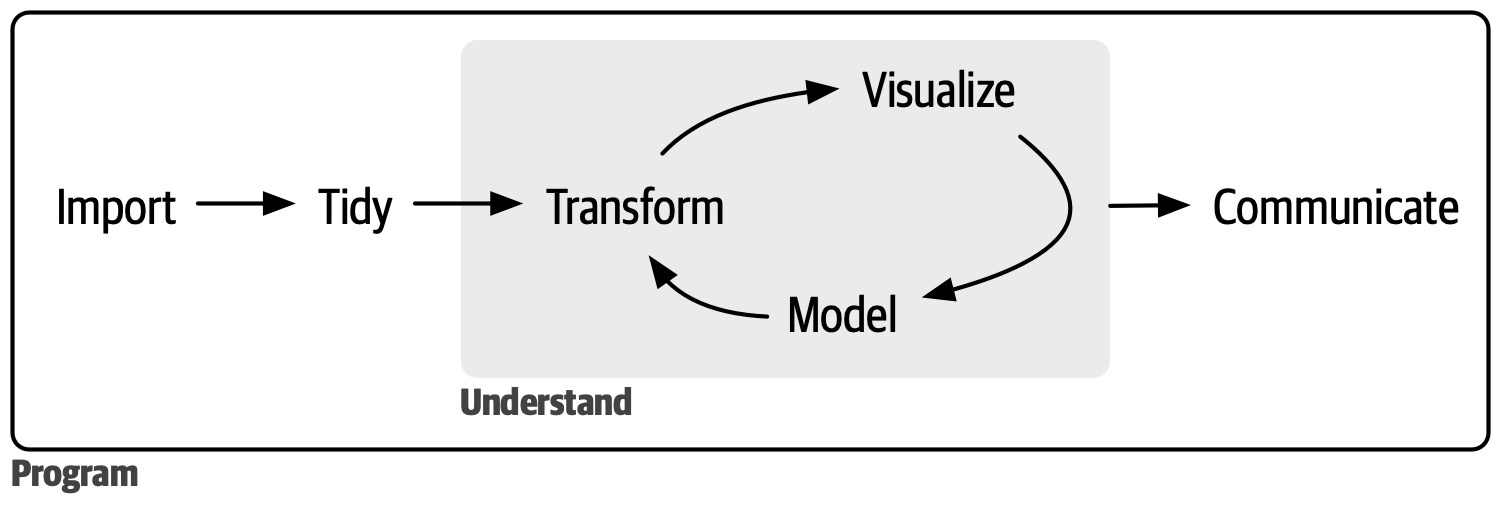
\includegraphics[width=5.57in,height=\textheight]{diagrams/data-science/base.png}

}

\caption{\label{fig-ds-diagram}在数据科学过程模型中,首先进行数据导入和整理。接下来,通过迭代循环的转换、
可视化和建模来理解数据。最后,通过与他人交流结果来完成整个过程。}

\end{figure}%

首先,必须将数据导入 (\textbf{import} ) R中。
这通常意味着你需要从文件、数据库或Web应用程序接口 (API)
中获取数据,并将其加载到R的一个数据框中。如
果无法将数据导入R,就无法在其上开展数据科学工作!

一旦导入了数据,还需对其进行整齐 (\textbf{tidy})。整
齐数据意味着以统一的形式存储数据,使数据集的语义与其存储方式相匹配。简
而言之,当数据整齐时,每一列都是一个变量,每一行都是一个观测值。整
齐的数据很重要,因为结构一致使你可以将精力集中在回答有关数据的问题上,而不是努力将数据转换成适合不同功能的正确形式。

当数据整齐完成后,通常下一步是数据转换 (\textbf{transform})。转
换包括缩小感兴趣的观察值的范围(如一个城市的所有人或去年的所有数据)、根据现有变量创建新变量(如根据距离和时间计算速度),以及计算一组数据的统计量(如计数或平均值)。整
齐和转换统称为数据清洗 (wrangling)
因为将数据以自然的形式处理通常感觉像是一场战斗!

当有了由所需变量组成的整齐数据后,就可利用两个主要的知识生成引擎:可视化和建模。它
们的优缺点互补,因此任何数据分析都可反复利用它们。

可视化 (\textbf{Visualization}) 是一项基本的人类活动。一
个好的可视化会显示你没有预料到的东西,或者提出关于数据的新问题。一
个好的可视化还可能暗示你问错了问题,或者你需要收集不同的数据。可
视化可能会让你感到惊讶,但它们的扩展性并不强,因为它们需要人来解释。

建模 (\textbf{Models}) 是对可视化的补充。一
旦你的问题足够精准,你就可以用一个模型来回答。模
型基本上是数学或计算工具,因此它们通常具有良好的可扩展性。即
使模型扩展性不佳,买更多的电脑通常比买更多的大脑要便宜!但
每个模型都需要做假设,而且就其本质而言,模型不能质疑自己的假设。这
意味着一个模型不能从根本上给你带来惊喜。

数据科学的最后一步是交流
(\textbf{communication}),这是每个数据分析项目中绝对重要的步骤。除
非你能够与他人交流你的结果,否则无论模型和可视化如何帮助你很好地理解数据都无足轻重。

围绕所有这些工具的是编程 (\textbf{programming})。编
程是一种综合工具,在数据科学项目的几乎每个部分都要用到。要
成为一名成功的数据科学家,你不需要成为一名专业的程序员,但是学习更多的编程知识是值得的,因为成为一名好的程序员可以让你解决常规问题自动化,并使解决新问题变得更轻松。

你将在每个数据科学项目中用到这些工具,但对大多数项目来说这些工具还不够。这
里有一个大致的80/20规则:你可以使用你在本书中学到的工具来解决项目中大约80\%的问题,但剩下的20\%需要其他工具来处理。在
本书中我们将为你提供了解更多信息的资源。

\section*{本书的组织结构}\label{ux672cux4e66ux7684ux7ec4ux7ec7ux7ed3ux6784}
\addcontentsline{toc}{section}{本书的组织结构}

\markright{本书的组织结构}

前面关于数据科学工具的描述大致上是按照数据分析中使用的顺序组织的
(当然,你会多次重复这个过程)。然
而,根据我们的经验,首先学习数据导入和整理是次优的,因为80\%的时间是常规的且无聊的,而另外20\%的时间是不寻常且令人沮丧的。这
不是学习新学科的好起点!相
反,我们将从已经导入和整理的数据的可视化和转换开始。这
样,当你处理和整理自己的数据时,你的动力就会保持高涨,因为你知道痛苦是值得的。

在每一章中,我们尽量遵循一个一致的模式:从一些鼓舞人心的例子开始,让你可以看到更大的图景,然后再深入到细节中。书
中的每一部分都配有练习来帮助你练习所学的知识。虽
然跳过练习很有诱惑力,但没有比在实际问题上练习更好的学习方法了。

\section*{学不到的内容}\label{ux5b66ux4e0dux5230ux7684ux5185ux5bb9}
\addcontentsline{toc}{section}{学不到的内容}

\markright{学不到的内容}

有几个重要的主题这本书没有涉及。我
们认为坚持不懈地专注于最基本的东西是很重要的,这样你就能尽快开始行动。这
也表明这本书不可能涵盖每一个重要主题。

\subsection*{建模}\label{ux5efaux6a21}
\addcontentsline{toc}{subsection}{建模}

对于数据科学来说建模是非常重要的,但这是一个很大的主题。而
不幸的是,我们没有足够的空间在这里给予它应有的篇幅。要
了解更多关于建模的知识,我们强烈推荐由我们的同事Max Kuhn和Julia
Silge的编写的\href{https://www.tmwr.org}{Tidy Modeling with R} 。本
书将向你介绍tidymodels包家族,正如你从名称中猜到的那样,它与我们在本书中使用的tidyverse包共享许多约定。

\subsection*{大数据}\label{ux5927ux6570ux636e}
\addcontentsline{toc}{subsection}{大数据}

本书主要关注小型内存数据集。这
是一个正确的起点,因为只有在你具备处理小数据的经验后,才能处理大数据。本
书大部分内容所提供的工具都可以用来轻松处理数百兆字节的数据,稍加注意它们甚至可以处理几GB的数据。我
们还将向你展示如何从数据库和\emph{Parquet}文件中获取数据,这两种文件通常用于存储大数据。你
不一定能够处理整个数据集,但这不是问题,因为你只需要一个子集或者子样本来回答你感兴趣的问题。

如果你经常需要处理更大的数据 (比如说10-100GB),我们建议你进一步了解
\href{https://github.com/Rdatatable/data.table}{data.table}。我
们在这里不做讲解,因为它使用的接口与tidyverse不同,需要学习一些不同的约定。然
而它的速度非常快,如果你正在处理大数据,那么它的优异性能表现值得你投入一些时间来学习它。

\subsection*{Python、Julia和其他编程语言}\label{pythonjuliaux548cux5176ux4ed6ux7f16ux7a0bux8bedux8a00}
\addcontentsline{toc}{subsection}{Python、Julia和其他编程语言}

在这本书中,你不会学到任何关于Python、Julia或其他对数据科学有用的编程语言的知识。这
并不是因为我们认为这些工具不好,它们很优秀!在
实践中,大多数数据科学团队使用混合语言,通常至少是R和Python。但
我们坚信,最好一次只掌握一种工具,R就是一个很好的起点。

\section*{预备知识}\label{ux9884ux5907ux77e5ux8bc6}
\addcontentsline{toc}{section}{预备知识}

\markright{预备知识}

为了让你从这本书中获得最大的收益,我们对你已经知道的内容做了一些假设。你
应该对数字有一定的了解,如果你已经有一些基本的编程经验,那将会很有帮助。如
果你以前从未编过程,你会发现Garrett编写的\href{https://rstudio-education.github.io/hopr/}{Hands
on Programming with R} 是这本书的一个有益补充。

运行这本书中的代码,你需要四样东西:R、RStudio,一个名为tidyverse的R包集合以及其他几个包。包
是可重现R代码的基本单元。它
们包括可重用的函数、描述如何使用它们的文档以及样本数据。

\subsection*{R}\label{r}
\addcontentsline{toc}{subsection}{R}

要下载R,请访问CRAN (the \textbf{c}omprehensive \textbf{R}
\textbf{a}rchive \textbf{n}etwork) \url{https://cloud.r-project.org}。R
新的主要版本每年发布一次,也会发布2-3个次要版本,建议定期更新。升
级可能会有点麻烦,特别是主要版本,需要你重新安装所有的包,但是拖延只会让情况变得更糟。我
们建议本书使用R4.2.0或更高版本。

\subsection*{RStudio}\label{rstudio}
\addcontentsline{toc}{subsection}{RStudio}

RStudio 是一个用于编程的集成开发环境,你可以从
\url{https://posit.co/download/rstudio-desktop/}下载。\\
RStudio每年更新几次,当新版本发布时,它会自动通知你,所以不需要定期查看,但最好定期升级,以利用最新和最强大的功能。对
于这本书,请确保你至少有RStudio 2022.02.0版本。

当你启动RStudio后,如 图~\ref{fig-rstudio-console}
,在界面中你会看到两个关键区域:控制台面板和输出面板。现
在你需要知道的是,你在控制台面板中输入R代码,然后按回车键来运行它。随
着我们的逐步深入,你会学到更多\footnote{If you'd like a comprehensive
  overview of all of RStudio's features, see the RStudio User Guide at
  \url{https://docs.posit.co/ide/user}.}。

\begin{figure}

\centering{

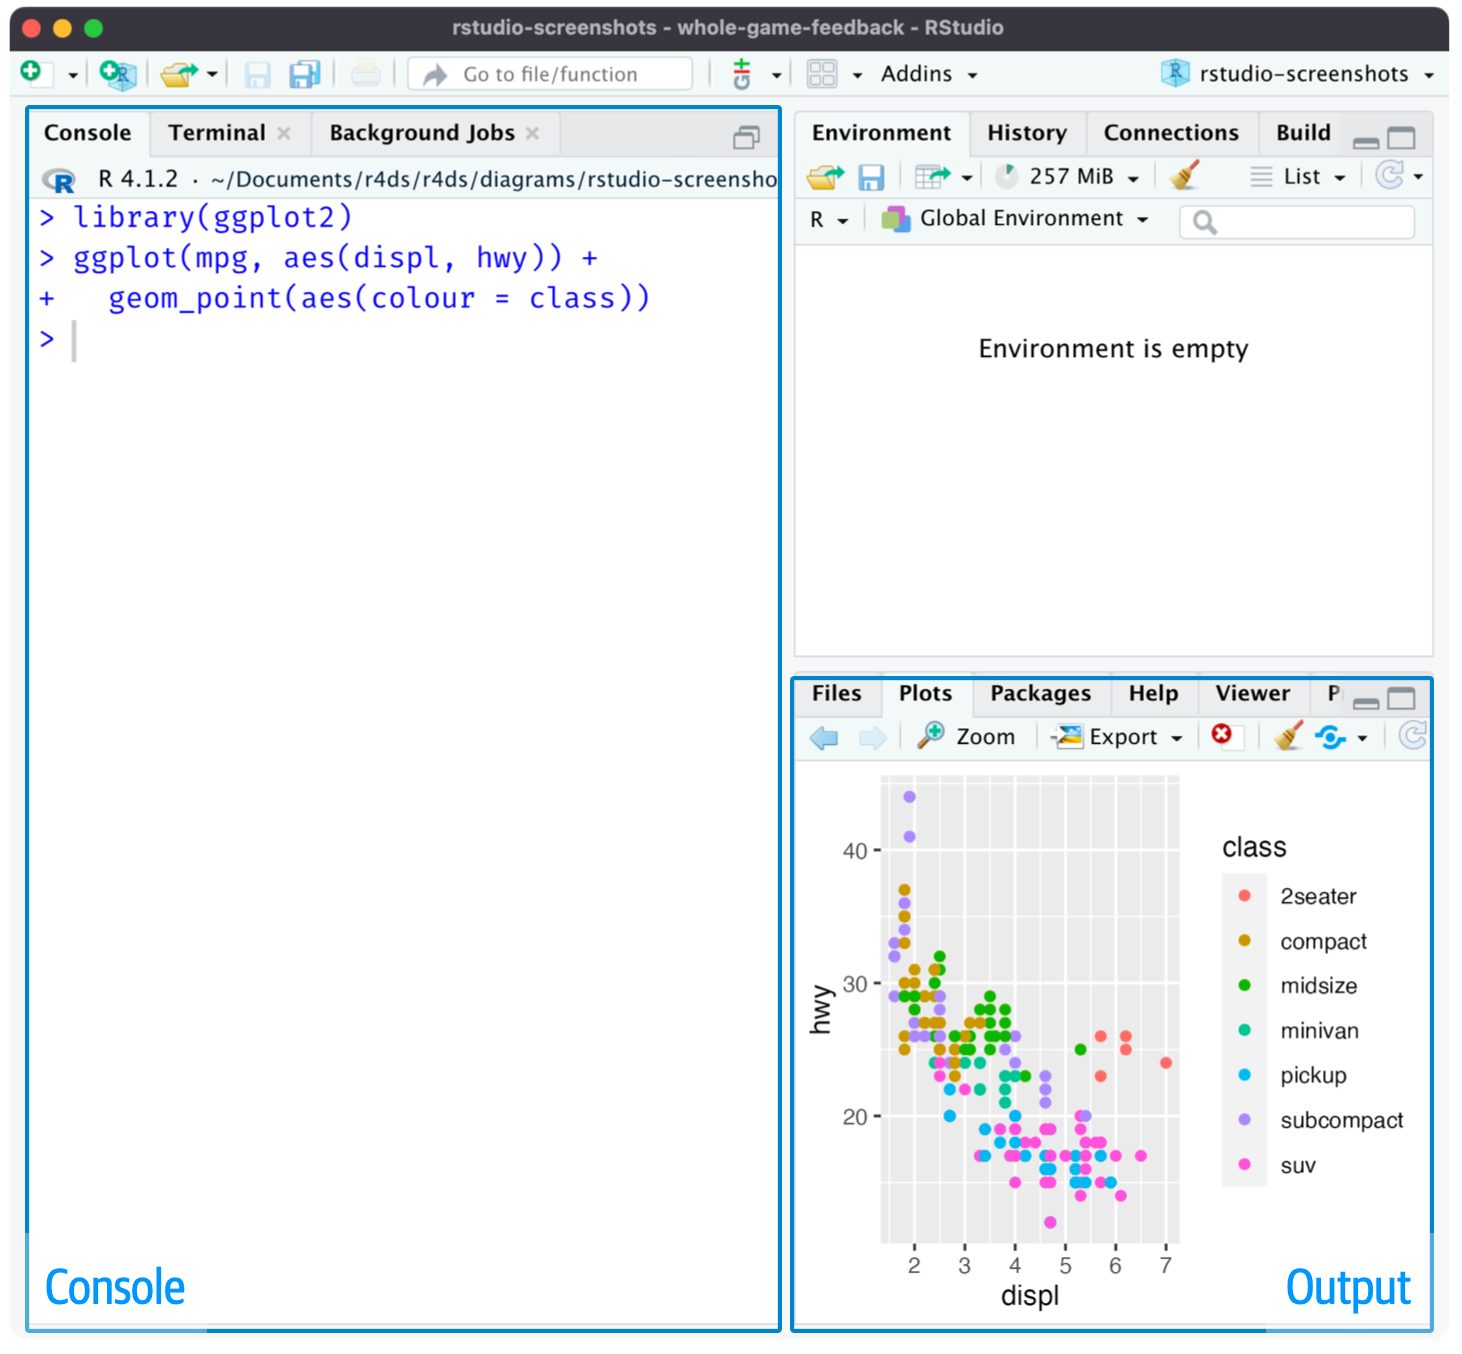
\includegraphics[width=5.41in,height=\textheight]{diagrams/rstudio/console.png}

}

\caption{\label{fig-rstudio-console}RStudio IDE
有两个关键区域:在左侧的控制台面板中输入R代码,
在右侧的输出面板中查看图形。}

\end{figure}%

\subsection*{Tidyverse}\label{tidyverse}
\addcontentsline{toc}{subsection}{Tidyverse}

你还需要安装一些R包。R
包是函数、数据和文档的集合,它扩展了基础R的功能。使
用包是成功使用R的关键。你
在本书中学习的大多数包都是所谓tidyverse的一部分。t
idyverse中的所有包都共享数据和R编程的共同理念,并被精心安排在一起协同工作。

你可以使用一行代码安装完整的tidyverse包:

\begin{Shaded}
\begin{Highlighting}[]
\FunctionTok{install.packages}\NormalTok{(}\StringTok{"tidyverse"}\NormalTok{)}
\end{Highlighting}
\end{Shaded}

在你的计算机上,在控制台中键入这行代码,然后按enter键运行它,R将从CRAN下载软件包并安装到你的计算机上。

在使用\texttt{library()}加载包之前,你无法使用包中的函数、对象或帮助文件。一
旦安装了一个包,你可以使用\texttt{library()} 来加载它:

\begin{Shaded}
\begin{Highlighting}[]
\FunctionTok{library}\NormalTok{(tidyverse)}
\CommentTok{\#\textgreater{} {-}{-} Attaching core tidyverse packages {-}{-}{-}{-}{-}{-}{-}{-}{-}{-}{-}{-}{-}{-}{-}{-}{-}{-}{-}{-}{-} tidyverse 2.0.0 {-}{-}}
\CommentTok{\#\textgreater{} v dplyr     1.1.4     v readr     2.1.5}
\CommentTok{\#\textgreater{} v forcats   1.0.0     v stringr   1.5.1}
\CommentTok{\#\textgreater{} v ggplot2   3.5.0     v tibble    3.2.1}
\CommentTok{\#\textgreater{} v lubridate 1.9.3     v tidyr     1.3.1}
\CommentTok{\#\textgreater{} v purrr     1.0.2     }
\CommentTok{\#\textgreater{} {-}{-} Conflicts {-}{-}{-}{-}{-}{-}{-}{-}{-}{-}{-}{-}{-}{-}{-}{-}{-}{-}{-}{-}{-}{-}{-}{-}{-}{-}{-}{-}{-}{-}{-}{-}{-}{-}{-}{-}{-}{-}{-} tidyverse\_conflicts() {-}{-}}
\CommentTok{\#\textgreater{} x dplyr::filter() masks stats::filter()}
\CommentTok{\#\textgreater{} x dplyr::lag()    masks stats::lag()}
\CommentTok{\#\textgreater{} i Use the conflicted package (\textless{}http://conflicted.r{-}lib.org/\textgreater{}) to force all conflicts to become errors}
\end{Highlighting}
\end{Shaded}

这告诉你,tidyverse加载了9个包:
dplyr、forcats、ggplot2、lubrid、purrr、reader、stringr、tibble和tidyr。它
们被认为是tidyverse的核心,因为几乎在所有数据分析中都会用到它们。

tidyverse中的包变化相当频繁。可
以通过运行\texttt{tidyverse\_update()}查看是否有可用的更新。

\subsection*{其他包}\label{ux5176ux4ed6ux5305}
\addcontentsline{toc}{subsection}{其他包}

还有许多其他优秀的软件包,它们不是tidyverse的一部分,因为它们解决了不同领域的问题,或者是用不同的基本原则设计的。这
不会让它们变得更好或更糟,这只会让它们与众不同。换 句话说,对
tidyverse的补充不是messyverse,而是由相互关联的包组成的许多其他universes。随
着你使用R处理更多的数据科学项目,你将学习新的包和新的数据思考方式。

在本书中,我们将使用许多来自tidyverse之外的包。例
如以下的包为我们在学习R的过程中提供了有趣的数据集:

\begin{Shaded}
\begin{Highlighting}[]
\FunctionTok{install.packages}\NormalTok{(}
  \FunctionTok{c}\NormalTok{(}\StringTok{"arrow"}\NormalTok{, }\StringTok{"babynames"}\NormalTok{, }\StringTok{"curl"}\NormalTok{, }\StringTok{"duckdb"}\NormalTok{, }\StringTok{"gapminder"}\NormalTok{, }
    \StringTok{"ggrepel"}\NormalTok{, }\StringTok{"ggridges"}\NormalTok{, }\StringTok{"ggthemes"}\NormalTok{, }\StringTok{"hexbin"}\NormalTok{, }\StringTok{"janitor"}\NormalTok{, }\StringTok{"Lahman"}\NormalTok{, }
    \StringTok{"leaflet"}\NormalTok{, }\StringTok{"maps"}\NormalTok{, }\StringTok{"nycflights13"}\NormalTok{, }\StringTok{"openxlsx"}\NormalTok{, }\StringTok{"palmerpenguins"}\NormalTok{, }
    \StringTok{"repurrrsive"}\NormalTok{, }\StringTok{"tidymodels"}\NormalTok{, }\StringTok{"writexl"}\NormalTok{)}
\NormalTok{  )}
\end{Highlighting}
\end{Shaded}

我们还将使用一些其他包作为单独的示例。你
现在不需要安装它们,只要记住每当你看到这样的错误时:

\begin{Shaded}
\begin{Highlighting}[]
\FunctionTok{library}\NormalTok{(ggrepel)}
\CommentTok{\#\textgreater{} Error in library(ggrepel) : there is no package called ‘ggrepel’}
\end{Highlighting}
\end{Shaded}

你需要运行 \texttt{install.packages("ggrepel")} 来安装这个包。

\section*{运行R代码}\label{ux8fd0ux884crux4ee3ux7801}
\addcontentsline{toc}{section}{运行R代码}

\markright{运行R代码}

前一节向你展示了几个运行R代码的示例,书中的代码看起来是这样的:

\begin{Shaded}
\begin{Highlighting}[]
\DecValTok{1} \SpecialCharTok{+} \DecValTok{2}
\CommentTok{\#\textgreater{} [1] 3}
\end{Highlighting}
\end{Shaded}

如果你在本地控制台中运行相同的代码,它看起来像这样:

\begin{verbatim}
> 1 + 2
[1] 3
\end{verbatim}

有两个主要区别:在控制台中,你在\texttt{\textgreater{}}之后键入,\texttt{\textgreater{}}称为提示符。我
们在书中没有显示提示符。在
本书中,输出用\texttt{\#\textgreater{}}注释掉。在
控制台中,它直接出现在代码之后。这
两个区别意味着,如果你使用的是电子书,你可以轻松地从书中复制代码并将其粘贴到控制台。

在本书中,我们使用一致的约定来引用代码:

\begin{itemize}
\item
  函数用代码字体显示,后面跟着圆括号,如 \texttt{sum()} 或
  \texttt{mean()};
\item
  其他R对象 (例如数据或函数参数) 用代码字体,没有圆括号, 如
  \texttt{flights} 或 \texttt{x}.
\item
  有时,为了明确对象来自哪个包,to make it clear which package an object
  comes from, 我们使用包名后面加两个冒号,如 \texttt{dplyr::mutate()} 或
  \texttt{nycflights13::flights}。这 也是有效的R代码。
\end{itemize}

\section*{致谢}\label{ux81f4ux8c22-1}
\addcontentsline{toc}{section}{致谢}

\markright{致谢}

这本书不仅仅是Hadley、我和Garrett的作品,也是我们与R社区许多人(面对面和在线)多次交谈的结果。非
常感谢与你们所有人的交流,非常感谢!

这本书是公开编写的,许多人通过拉取请求(pull
requests)做出了贡献。特别感谢通过GitHub拉取请求的259 位贡献者
(按用户名字母顺序): @a-rosenberg, Tim Becker (@a2800276), Abinash
Satapathy (@Abinashbunty), Adam Gruer (@adam-gruer), adi pradhan
(@adidoit), A. s. (@Adrianzo), Aep Hidyatuloh (@aephidayatuloh), Andrea
Gilardi (@agila5), Ajay Deonarine (@ajay-d), @AlanFeder, Daihe Sui
(@alansuidaihe), @alberto-agudo, @AlbertRapp, @aleloi, pete (@alonzi),
Alex (@ALShum), Andrew M. (@amacfarland), Andrew Landgraf (@andland),
@andyhuynh92, Angela Li (@angela-li), Antti Rask (@AnttiRask), LOU Xun
(@aquarhead), @ariespirgel, @august-18, Michael Henry (@aviast), Azza
Ahmed (@azzaea), Steven Moran (@bambooforest), Brian G. Barkley
(@BarkleyBG), Mara Averick (@batpigandme), Oluwafemi OYEDELE (@BB1464),
Brent Brewington (@bbrewington), Bill Behrman (@behrman), Ben Herbertson
(@benherbertson), Ben Marwick (@benmarwick), Ben Steinberg
(@bensteinberg), Benjamin Yeh (@bentyeh), Betul Turkoglu
(@betulturkoglu), Brandon Greenwell (@bgreenwell), Bianca Peterson
(@BinxiePeterson), Birger Niklas (@BirgerNi), Brett Klamer (@bklamer),
@boardtc, Christian (@c-hoh), Caddy (@caddycarine), Camille V Leonard
(@camillevleonard), @canovasjm, Cedric Batailler (@cedricbatailler),
Christina Wei (@christina-wei), Christian Mongeau (@chrMongeau), Cooper
Morris (@coopermor), Colin Gillespie (@csgillespie), Rademeyer Vermaak
(@csrvermaak), Chloe Thierstein (@cthierst), Chris Saunders (@ctsa),
Abhinav Singh (@curious-abhinav), Curtis Alexander (@curtisalexander),
Christian G. Warden (@cwarden), Charlotte Wickham (@cwickham), Kenny
Darrell (@darrkj), David Kane (@davidkane9), David (@davidrsch), David
Rubinger (@davidrubinger), David Clark (@DDClark), Derwin McGeary
(@derwinmcgeary), Daniel Gromer (@dgromer), @Divider85, @djbirke,
Danielle Navarro (@djnavarro), Russell Shean (@DOH-RPS1303), Zhuoer Dong
(@dongzhuoer), Devin Pastoor (@dpastoor), @DSGeoff, Devarshi Thakkar
(@dthakkar09), Julian During (@duju211), Dylan Cashman (@dylancashman),
Dirk Eddelbuettel (@eddelbuettel), Edwin Thoen (@EdwinTh), Ahmed
El-Gabbas (@elgabbas), Henry Webel (@enryH), Ercan Karadas (@ercan7),
Eric Kitaif (@EricKit), Eric Watt (@ericwatt), Erik Erhardt
(@erikerhardt), Etienne B. Racine (@etiennebr), Everett Robinson
(@evjrob), @fellennert, Flemming Miguel (@flemmingmiguel), Floris
Vanderhaeghe (@florisvdh), @funkybluehen, @gabrivera, Garrick Aden-Buie
(@gadenbuie), Peter Ganong (@ganong123), Gerome Meyer (@GeroVanMi), Gleb
Ebert (@gl-eb), Josh Goldberg (@GoldbergData), bahadir cankardes
(@gridgrad), Gustav W Delius (@gustavdelius), Hao Chen (@hao-trivago),
Harris McGehee (@harrismcgehee), @hendrikweisser, Hengni Cai
(@hengnicai), Iain (@Iain-S), Ian Sealy (@iansealy), Ian Lyttle
(@ijlyttle), Ivan Krukov (@ivan-krukov), Jacob Kaplan (@jacobkap), Jazz
Weisman (@jazzlw), John Blischak (@jdblischak), John D. Storey
(@jdstorey), Gregory Jefferis (@jefferis), Jeffrey Stevens
(@JeffreyRStevens), 蒋雨蒙 (@JeldorPKU), Jennifer (Jenny) Bryan
(@jennybc), Jen Ren (@jenren), Jeroen Janssens (@jeroenjanssens),
@jeromecholewa, Janet Wesner (@jilmun), Jim Hester (@jimhester), JJ Chen
(@jjchern), Jacek Kolacz (@jkolacz), Joanne Jang (@joannejang),
@johannes4998, John Sears (@johnsears), @jonathanflint, Jon Calder
(@jonmcalder), Jonathan Page (@jonpage), Jon Harmon (@jonthegeek),
JooYoung Seo (@jooyoungseo), Justinas Petuchovas (@jpetuchovas), Jordan
(@jrdnbradford), Jeffrey Arnold (@jrnold), Jose Roberto Ayala Solares
(@jroberayalas), Joyce Robbins (@jtr13), @juandering, Julia Stewart
Lowndes (@jules32), Sonja (@kaetschap), Kara Woo (@karawoo), Katrin
Leinweber (@katrinleinweber), Karandeep Singh (@kdpsingh), Kevin Perese
(@kevinxperese), Kevin Ferris (@kferris10), Kirill Sevastyanenko
(@kirillseva), Jonathan Kitt (@KittJonathan), @koalabearski, Kirill
Müller (@krlmlr), Rafał Kucharski (@kucharsky), Kevin Wright (@kwstat),
Noah Landesberg (@landesbergn), Lawrence Wu (@lawwu), @lindbrook, Luke W
Johnston (@lwjohnst86), Kara de la Marck (@MarckK), Kunal Marwaha
(@marwahaha), Matan Hakim (@matanhakim), Matthias Liew (@MatthiasLiew),
Matt Wittbrodt (@MattWittbrodt), Mauro Lepore (@maurolepore), Mark
Beveridge (@mbeveridge), @mcewenkhundi, mcsnowface, PhD (@mcsnowface),
Matt Herman (@mfherman), Michael Boerman (@michaelboerman), Mitsuo
Shiota (@mitsuoxv), Matthew Hendrickson (@mjhendrickson), @MJMarshall,
Misty Knight-Finley (@mkfin7), Mohammed Hamdy (@mmhamdy), Maxim Nazarov
(@mnazarov), Maria Paula Caldas (@mpaulacaldas), Mustafa Ascha
(@mustafaascha), Nelson Areal (@nareal), Nate Olson (@nate-d-olson),
Nathanael (@nateaff), @nattalides, Ned Western (@NedJWestern), Nick
Clark (@nickclark1000), @nickelas, Nirmal Patel (@nirmalpatel), Nischal
Shrestha (@nischalshrestha), Nicholas Tierney (@njtierney), Jakub
Nowosad (@Nowosad), Nick Pullen (@nstjhp), @olivier6088, Olivier
Cailloux (@oliviercailloux), Robin Penfold (@p0bs), Pablo E. Garcia
(@pabloedug), Paul Adamson (@padamson), Penelope Y (@penelopeysm), Peter
Hurford (@peterhurford), Peter Baumgartner (@petzi53), Patrick Kennedy
(@pkq), Pooya Taherkhani (@pooyataher), Y. Yu (@PursuitOfDataScience),
Radu Grosu (@radugrosu), Ranae Dietzel (@Ranae), Ralph Straumann
(@rastrau), Rayna M Harris (@raynamharris), @ReeceGoding, Robin
Gertenbach (@rgertenbach), Jajo (@RIngyao), Riva Quiroga (@rivaquiroga),
Richard Knight (@RJHKnight), Richard Zijdeman (@rlzijdeman),
@robertchu03, Robin Kohrs (@RobinKohrs), Robin (@Robinlovelace), Emily
Robinson (@robinsones), Rob Tenorio (@robtenorio), Rod Mazloomi
(@RodAli), Rohan Alexander (@RohanAlexander), Romero Morais
(@RomeroBarata), Albert Y. Kim (@rudeboybert), Saghir (@saghirb), Hojjat
Salmasian (@salmasian), Jonas (@sauercrowd), Vebash Naidoo
(@sciencificity), Seamus McKinsey (@seamus-mckinsey), @seanpwilliams,
Luke Smith (@seasmith), Matthew Sedaghatfar (@sedaghatfar), Sebastian
Kraus (@sekR4), Sam Firke (@sfirke), Shannon Ellis (@ShanEllis),
@shoili, Christian Heinrich (@Shurakai), S'busiso Mkhondwane
(@sibusiso16), SM Raiyyan (@sm-raiyyan), Jakob Krigovsky (@sonicdoe),
Stephan Koenig (@stephan-koenig), Stephen Balogun (@stephenbalogun),
Steven M. Mortimer (@StevenMMortimer), Stéphane Guillou (@stragu), Sulgi
Kim (@sulgik), Sergiusz Bleja (@svenski), Tal Galili (@talgalili), Alec
Fisher (@Taurenamo), Todd Gerarden (@tgerarden), Tom Godfrey
(@thomasggodfrey), Tim Broderick (@timbroderick), Tim Waterhouse
(@timwaterhouse), TJ Mahr (@tjmahr), Thomas Klebel (@tklebel), Tom Prior
(@tomjamesprior), Terence Teo (@tteo), @twgardner2, Ulrik Lyngs
(@ulyngs), Shinya Uryu (@uribo), Martin Van der Linden
(@vanderlindenma), Walter Somerville (@waltersom), @werkstattcodes, Will
Beasley (@wibeasley), Yihui Xie (@yihui), Yiming (Paul) Li (@yimingli),
@yingxingwu, Hiroaki Yutani (@yutannihilation), Yu Yu Aung (@yuyu-aung),
Zach Bogart (@zachbogart), @zeal626, Zeki Akyol (@zekiakyol).

\section*{版权}\label{ux7248ux6743}
\addcontentsline{toc}{section}{版权}

\markright{版权}

本书的在线版本访问
\url{https://r4ds.hadley.nz},在纸质书印刷期间本书将继续发展。本
书的源代码可在 \url{https://github.com/hadley/r4ds}获取。 本书由
\href{https://quarto.org}{Quarto}提供支持,这使得编写结合了文本和可执行代码的书变得很容易。

\part{全貌概览}

本书这一部分的目的是让你快速浏览数据科学的主要工具:\textbf{导入}、\textbf{整理}、\textbf{转换}和\textbf{可视化}数据,如
图~\ref{fig-ds-whole-game} 所示。我
们将向你展示数据科学的``全貌'',为你提供各主要部分的足够内容,以便你能够处理真实
(尽管可能简单) 的数据集。本
书后面的部分将深入探讨这些主题,从而增加你解决数据科学挑战的范围。

\begin{figure}

\centering{

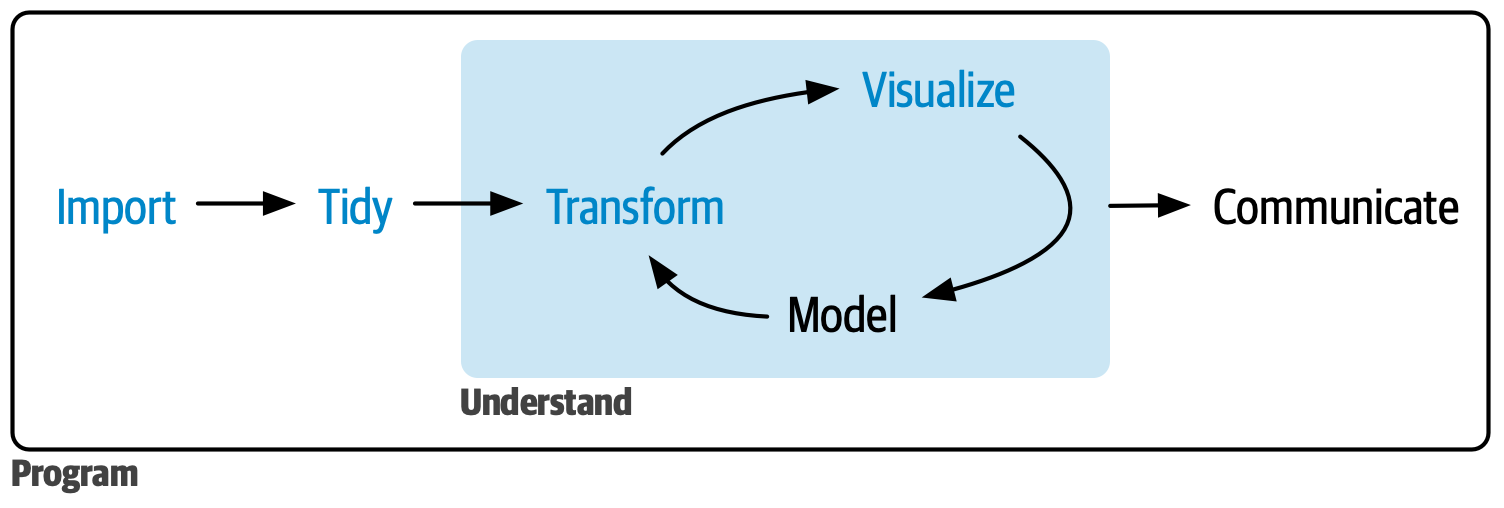
\includegraphics[width=5.57in,height=\textheight]{diagrams/data-science/whole-game.png}

}

\caption{\label{fig-ds-whole-game}在本书的这一节中,你将学习如何导入、整齐、转换和可视化数据;编程贯穿于各个过程。}

\end{figure}%

数据科学工具包含四章内容:

\begin{itemize}
\item
  可视化是学习R编程非常好的起点,因为它的回报是如此明显:你可以制作优雅且信息丰富的图形,以帮助你理解数据。在
  章节~\ref{sec-data-visualization}
  中,你将深入了解可视化,学习ggplot2图形的基本结构,以及将数据转换为图形的强大技术。
\item
  仅仅可视化通常是不够的,因此在 章节~\ref{sec-data-transform}
  中,你将学习关键函数,这些关键函数允许你选择重要变量、筛选关键观测值、创建新变量和计算汇总统计量。
\item
  在 章节~\ref{sec-data-tidy} 中,
  你将学习整理数据,这是一种致的数据存储方式,可以使数据转换、可视化和建模更容易。你
  将了解其基本原理,以及如何将数据整理成整齐的形式。
\item
  在转换和可视化数据之前,首先需要将数据导入R。在
  章节~\ref{sec-data-import} 中将学习把\texttt{.csv}
  文件导入R的基础知识。
\end{itemize}

在这些章节中,还有另外四章是关于R工作流程的。 在
章节~\ref{sec-workflow-basics},章节~\ref{sec-workflow-style} 和
章节~\ref{sec-workflow-scripts-projects}
中,你将学习编写和组织R代码的良好工作流程。从
长远来看这会让你更容易取得成功,因为它们将为你提供在处理实际项目时保持条理清晰的工具。最
后,章节~\ref{sec-workflow-getting-help} 将教你如何获得帮助并继续学习。

\chapter{数据可视化}\label{sec-data-visualization}

\section{引言}\label{ux5f15ux8a00}

\begin{quote}
``简单的图表比任何其他工具都能给数据分析师带来更多的信息.''

--- John Tukey
\end{quote}

R虽然有几个制图系统, 但ggplot2是最优雅、功能最多的一个系统。
ggplot2实现了描述和构建图形的连贯系统,即\textbf{图形的语法}。基
于ggplot2,通过学习一个系统并将其应用于许多地方,你可以做更多的事情而且速度更快。

本章将告诉你如何利用\textbf{ggplot2}可视化数据。我
们将首先创建一个简单的散点图,并用它引入ggplot2的基本构建模块,美学映射和几何对象。然
后将引导你可视化单个变量的分布以及可视化两个或多个变量之间的关系。最
后,保存所做的图和一些故障排除提示。

\subsection{必要条件}\label{ux5fc5ux8981ux6761ux4ef6}

本章重点介绍ggplot2, 它是tidyverse的核心包之一。要
访问本章中使用的数据集、帮助页和函数,请运行以下命令加载tidyverse:

\begin{Shaded}
\begin{Highlighting}[]
\FunctionTok{library}\NormalTok{(tidyverse)}
\CommentTok{\#\textgreater{} {-}{-} Attaching core tidyverse packages {-}{-}{-}{-}{-}{-}{-}{-}{-}{-}{-}{-}{-}{-}{-}{-}{-}{-}{-}{-}{-} tidyverse 2.0.0 {-}{-}}
\CommentTok{\#\textgreater{} v dplyr     1.1.4     v readr     2.1.5}
\CommentTok{\#\textgreater{} v forcats   1.0.0     v stringr   1.5.1}
\CommentTok{\#\textgreater{} v ggplot2   3.5.0     v tibble    3.2.1}
\CommentTok{\#\textgreater{} v lubridate 1.9.3     v tidyr     1.3.1}
\CommentTok{\#\textgreater{} v purrr     1.0.2     }
\CommentTok{\#\textgreater{} {-}{-} Conflicts {-}{-}{-}{-}{-}{-}{-}{-}{-}{-}{-}{-}{-}{-}{-}{-}{-}{-}{-}{-}{-}{-}{-}{-}{-}{-}{-}{-}{-}{-}{-}{-}{-}{-}{-}{-}{-}{-}{-} tidyverse\_conflicts() {-}{-}}
\CommentTok{\#\textgreater{} x dplyr::filter() masks stats::filter()}
\CommentTok{\#\textgreater{} x dplyr::lag()    masks stats::lag()}
\CommentTok{\#\textgreater{} i Use the conflicted package (\textless{}http://conflicted.r{-}lib.org/\textgreater{}) to force all conflicts to become errors}
\end{Highlighting}
\end{Shaded}

这一行代码将加载 tidyverse,这是在几乎所有数据分析中都会用到的包。它
还告诉您tidyverse中的哪些函数与base
R中的函数冲突(或者与您可能加载的其他包冲突)\footnote{你可以通过使用冲突包(conflicted
  package)来消除该消息,并按需强制解决冲突,这在你加载更多包时变得尤为重要。可
  以在\href{https://conflicted.r-lib.org/}{https://conflicted.r-lib.org}上了解更多关于此的信息。}。

如果运行这段代码得到了错误信息,\texttt{there\ is\ no\ package\ called\ \textquotesingle{}tidyverse\textquotesingle{}},你需要先安装它,然后再次运行\texttt{library()}。

\begin{Shaded}
\begin{Highlighting}[]
\FunctionTok{install.packages}\NormalTok{(}\StringTok{"tidyverse"}\NormalTok{)}
\FunctionTok{library}\NormalTok{(tidyverse)}
\end{Highlighting}
\end{Shaded}

每个包只需要安装一次,但每次启动新会话时都需要加载它。

除了tidyverse,
我们还会用到\textbf{palmerpenguins}包,其中包含\texttt{penguins}数据集,记录了Palmer群岛三个岛屿上企鹅的身体测量数据,以及ggthemes包,它提供了一个色盲安全调色板。

\begin{Shaded}
\begin{Highlighting}[]
\FunctionTok{library}\NormalTok{(palmerpenguins)}
\FunctionTok{library}\NormalTok{(ggthemes)}
\end{Highlighting}
\end{Shaded}

\section{第一步}\label{ux7b2cux4e00ux6b65}

长鳍企鹅的体重是比短鳍企鹅的体重大还是小?你
可能已经有了答案,但试着让你的答案更精确。鳍
长和体重之间的关系是什么样的?正 相关还是负相关?线 性的还是非线性的?这
种关系会因企鹅的种类而异吗?企 鹅生活的岛屿不同会有影响吗?让
我们创建可视化图形来回答这些问题。

\subsection{\texorpdfstring{\texttt{penguins}
数据框}{penguins 数据框}}\label{penguins-ux6570ux636eux6846}

您可以使用包palmerpenguins(\texttt{palmerpenguins::penguins})中的\texttt{penguins}数据框架来测试你对这些问题的答案。数
据框架是变量(列)和观测(行)的矩形集合。\texttt{p} \texttt{enguins}
收录了344 条观测,由Kristen
Gorman博士和南极科考站帕尔默站收集并提供\footnote{Horst AM, Hill AP,
  Gorman KB (2020). palmerpenguins: Palmer Archipelago (Antarctica)
  penguin data. R package version 0.1.0.
  \url{https://allisonhorst.github.io/palmerpenguins/}. doi:
  10.5281/zenodo.3960218.}。

为了使讨论更容易,让我们定义一些术语:

\begin{itemize}
\item
  \textbf{变量}:变量是可以测量的数量、质量或属性。
\item
  \textbf{值}:值是你测量一个变量时的状态,一个变量的值可能会随着测量的不同而变化。
\item
  \textbf{观测}:观测是在相似条件下进行的一组测量(通常在相同的时间和相同的对象上进行)。一
  个观测会包含几个值,每个值与不同的变量相关联。我
  们有时将一个观测称为一个数据点。
\item
  \textbf{表格数据}:表格数据是一组值,每个值与一个变量和一个观测相关。如
  果将每个值放在自己的``单元格''中,将每个变量放在自己的列中,将每个观测放在自己的行中,则表格数据是整洁的。
\end{itemize}

在这种情况下,变量指的是所有企鹅的一个属性,而观测值指的是单个企鹅的所有属性。

在控制台中键入数据框的名称,R会输出其内容的预览。需
要注意的是这个预览的顶部显示有\texttt{tibble} 。在
tidyverse中,我们使用称为\textbf{tibbles}的特殊数据框,随后你将了解到更多。

\begin{Shaded}
\begin{Highlighting}[]
\NormalTok{penguins}
\CommentTok{\#\textgreater{} \# A tibble: 344 x 8}
\CommentTok{\#\textgreater{}   species island    bill\_length\_mm bill\_depth\_mm flipper\_length\_mm}
\CommentTok{\#\textgreater{}   \textless{}fct\textgreater{}   \textless{}fct\textgreater{}              \textless{}dbl\textgreater{}         \textless{}dbl\textgreater{}             \textless{}int\textgreater{}}
\CommentTok{\#\textgreater{} 1 Adelie  Torgersen           39.1          18.7               181}
\CommentTok{\#\textgreater{} 2 Adelie  Torgersen           39.5          17.4               186}
\CommentTok{\#\textgreater{} 3 Adelie  Torgersen           40.3          18                 195}
\CommentTok{\#\textgreater{} 4 Adelie  Torgersen           NA            NA                  NA}
\CommentTok{\#\textgreater{} 5 Adelie  Torgersen           36.7          19.3               193}
\CommentTok{\#\textgreater{} 6 Adelie  Torgersen           39.3          20.6               190}
\CommentTok{\#\textgreater{} \# i 338 more rows}
\CommentTok{\#\textgreater{} \# i 3 more variables: body\_mass\_g \textless{}int\textgreater{}, sex \textless{}fct\textgreater{}, year \textless{}int\textgreater{}}
\end{Highlighting}
\end{Shaded}

这个数据框包含 8 列。如
果使用\texttt{glimpse()},你可以看到所有变量和每个变量的前几个观察值。如
果你在使用RStudio,运行\texttt{View(penguins)}会打开一个交互式数据预览器。

\begin{Shaded}
\begin{Highlighting}[]
\FunctionTok{glimpse}\NormalTok{(penguins)}
\CommentTok{\#\textgreater{} Rows: 344}
\CommentTok{\#\textgreater{} Columns: 8}
\CommentTok{\#\textgreater{} $ species           \textless{}fct\textgreater{} Adelie, Adelie, Adelie, Adelie, Adelie, Adelie, A\textasciitilde{}}
\CommentTok{\#\textgreater{} $ island            \textless{}fct\textgreater{} Torgersen, Torgersen, Torgersen, Torgersen, Torge\textasciitilde{}}
\CommentTok{\#\textgreater{} $ bill\_length\_mm    \textless{}dbl\textgreater{} 39.1, 39.5, 40.3, NA, 36.7, 39.3, 38.9, 39.2, 34.\textasciitilde{}}
\CommentTok{\#\textgreater{} $ bill\_depth\_mm     \textless{}dbl\textgreater{} 18.7, 17.4, 18.0, NA, 19.3, 20.6, 17.8, 19.6, 18.\textasciitilde{}}
\CommentTok{\#\textgreater{} $ flipper\_length\_mm \textless{}int\textgreater{} 181, 186, 195, NA, 193, 190, 181, 195, 193, 190, \textasciitilde{}}
\CommentTok{\#\textgreater{} $ body\_mass\_g       \textless{}int\textgreater{} 3750, 3800, 3250, NA, 3450, 3650, 3625, 4675, 347\textasciitilde{}}
\CommentTok{\#\textgreater{} $ sex               \textless{}fct\textgreater{} male, female, female, NA, female, male, female, m\textasciitilde{}}
\CommentTok{\#\textgreater{} $ year              \textless{}int\textgreater{} 2007, 2007, 2007, 2007, 2007, 2007, 2007, 2007, 2\textasciitilde{}}
\end{Highlighting}
\end{Shaded}

\texttt{penguins} 中的变量包括:

\begin{enumerate}
\def\labelenumi{\arabic{enumi}.}
\item
  \texttt{species}:企鹅的种类(Adelie, Chinstrap, or Gentoo)
\item
  \texttt{flipper\_length\_mm}: 企鹅鳍的长度,以毫米为单位
\item
  \texttt{body\_mass\_g}: 企鹅的体重,以克为单位。
\end{enumerate}

要了解更多关于\texttt{penguins}的信息,可以运行\texttt{?penguins}打开帮助页面。

\subsection{最终目标}\label{sec-ultimate-goal}

本章的最终目标是在考虑企鹅种类的情况下重建展示企鹅鳍长和体重之间关系的视图。

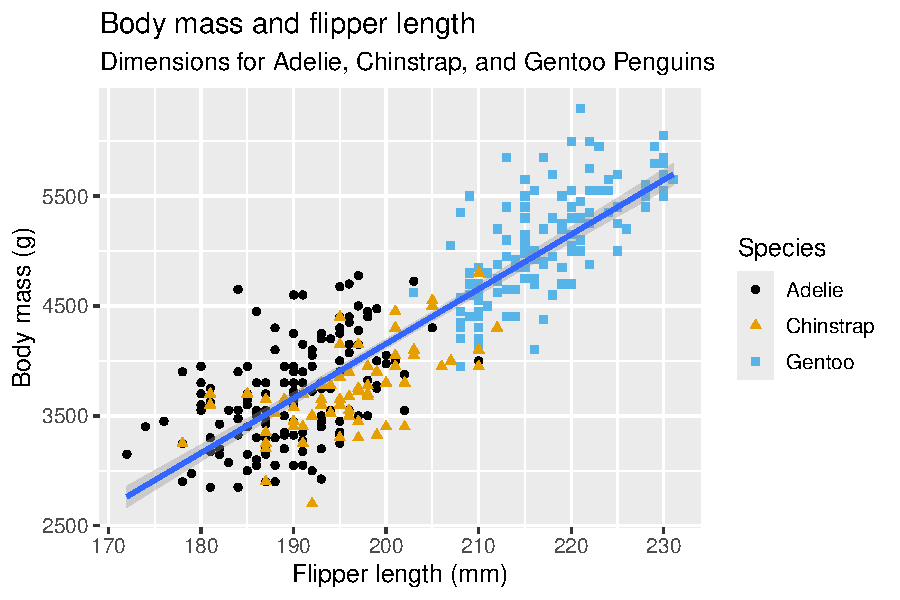
\includegraphics[width=18.75in,height=\textheight]{data-visualize_files/figure-pdf/unnamed-chunk-7-1.pdf}

\subsection{构建ggplot}\label{ux6784ux5efaggplot}

我们一步一步重建这个图。

利用ggplot2包的函数\texttt{ggplot()}绘图。首
先定义一个绘图对象,然后向其添加\textbf{图层}。
\texttt{ggplot()}的第一个参数是在图中使用的数据集,因此\texttt{ggplot(data\ =\ penguins)}创建了一个空图,用于显示\texttt{penguins}数据,但由于我们还没有告诉它如何可视化它,所以现在它是空的。这
不是一个可以让人动心的图,但你可以把它想象成一块空白画布,你可以在上面画出剩下的图层。

\begin{Shaded}
\begin{Highlighting}[]
\FunctionTok{ggplot}\NormalTok{(}\AttributeTok{data =}\NormalTok{ penguins)}
\end{Highlighting}
\end{Shaded}

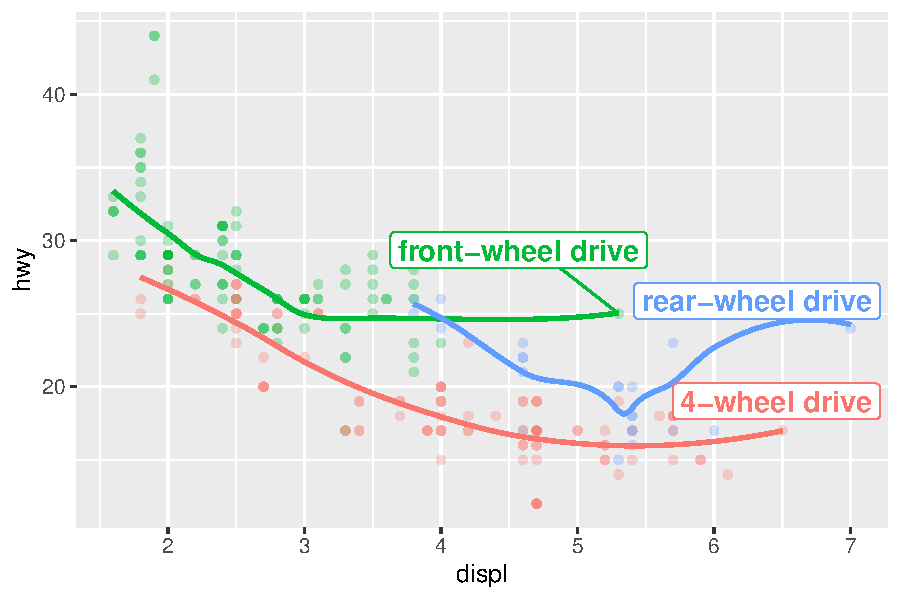
\includegraphics[width=18.75in,height=\textheight]{data-visualize_files/figure-pdf/unnamed-chunk-8-1.pdf}

接下来,需要告诉\texttt{ggplot()}如何将数据中的信息以视觉方式呈现。
\texttt{ggplot()}函数的\texttt{mapping}
参数定义了数据集中的变量如何映射到图表的视觉属性(\textbf{aesthetics})。
\texttt{mapping}参数总是在\texttt{aes()}函数中定义,而\texttt{aes()}的\texttt{x}和\texttt{y}参数则指定了哪些变量映射到x轴和y轴上。现
在,我们只将鳍长映射到\texttt{x}轴的美学属性上,将体重映射到\texttt{y}轴的美学属性上。g
gplot2会在数据参数中查找映射的变量,在这个例子中就是\texttt{penguins}。

下图显示了添加这些映射的结果。

\begin{Shaded}
\begin{Highlighting}[]
\FunctionTok{ggplot}\NormalTok{(}
  \AttributeTok{data =}\NormalTok{ penguins,}
  \AttributeTok{mapping =} \FunctionTok{aes}\NormalTok{(}\AttributeTok{x =}\NormalTok{ flipper\_length\_mm, }\AttributeTok{y =}\NormalTok{ body\_mass\_g)}
\NormalTok{)}
\end{Highlighting}
\end{Shaded}

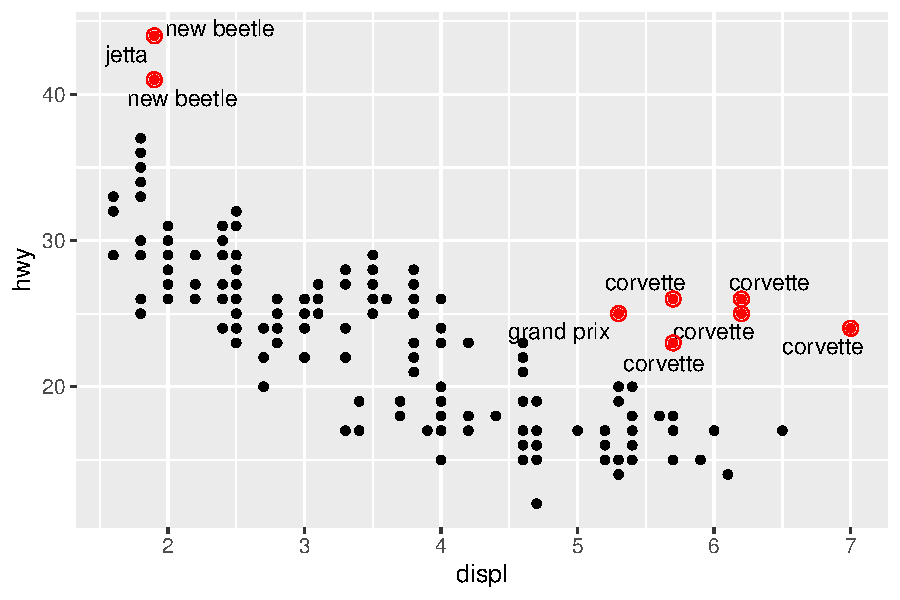
\includegraphics[width=18.75in,height=\textheight]{data-visualize_files/figure-pdf/unnamed-chunk-9-1.pdf}

空画布现在有了更多构造,我们已清楚知道鳍的长度在哪里显示(x轴),身体质量在哪里显示(y轴)。但
\texttt{penguins}本身还没有出现在图中。这
是因为在代码中,我们还没有明确说明如何在图上表示来自数据框架的观测。

为此我们需要定义一个\textbf{geom}(几何对象),geom是一个用来表示数据的图形。这
些geom在ggplot2中使用以\texttt{geom\_}开头的函数。我
们通常利用图使用的geom类型来描绘图形。例
如,条形图使用\texttt{geom\_bar()},折线图使用\texttt{geom\_line()},箱形图使用\texttt{geom\_boxplot()},散点图使用\texttt{geom\_point()},等等。

函数\texttt{geom\_point()}为图添加了一个点图层,从而创建了散点图。g
gplot2附带了许多geom函数,每个函数都为绘图添加不同类型的层。
你将在书中学到很多geom,特别是在 章节~\ref{sec-layers} 中。

\begin{Shaded}
\begin{Highlighting}[]
\FunctionTok{ggplot}\NormalTok{(}
  \AttributeTok{data =}\NormalTok{ penguins,}
  \AttributeTok{mapping =} \FunctionTok{aes}\NormalTok{(}\AttributeTok{x =}\NormalTok{ flipper\_length\_mm, }\AttributeTok{y =}\NormalTok{ body\_mass\_g)}
\NormalTok{) }\SpecialCharTok{+}
  \FunctionTok{geom\_point}\NormalTok{()}
\CommentTok{\#\textgreater{} Warning: Removed 2 rows containing missing values or values outside the scale range}
\CommentTok{\#\textgreater{} (\textasciigrave{}geom\_point()\textasciigrave{}).}
\end{Highlighting}
\end{Shaded}

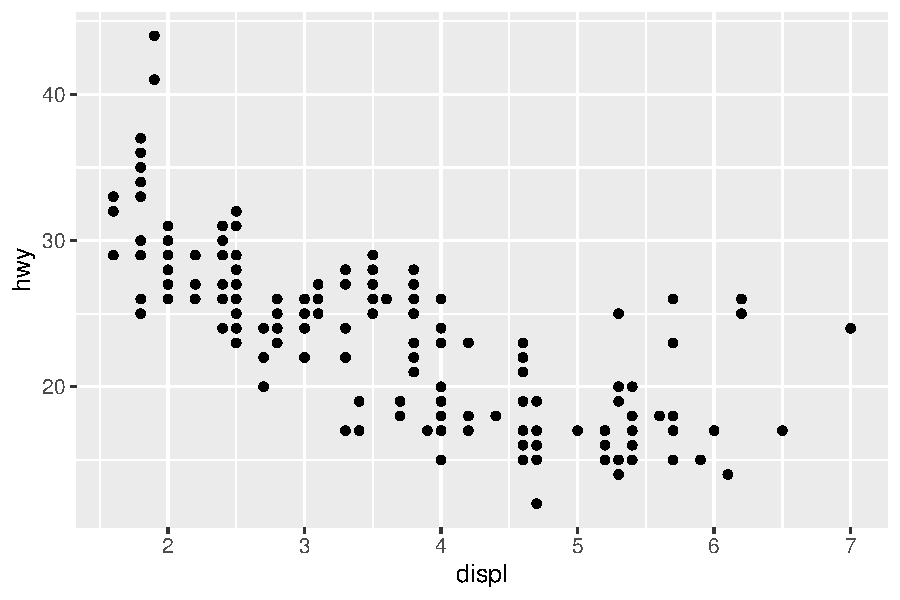
\includegraphics[width=18.75in,height=\textheight]{data-visualize_files/figure-pdf/unnamed-chunk-10-1.pdf}

现在我们得到了一些我们可能认为是``散点图''的东西,但这还不是我们的``最终目标''。但
利用这个图可以开始回答当初激发我们探索兴趣的问题:``鳍长和体重之间的关系是什么?''
这种关系似乎是正的(随着鳍的长度增加体重也会增加),呈线性(这些点聚集在一条直线上,而不是一条曲线),且线性关系比较强(在这样一条直线周围没有太多的发散点)。就体重而言,脚蹼较长的企鹅通常体型较大。

在添加更多图层到这个图之前,让我们暂停一下,回顾一下我们得到的警告信息:

\begin{quote}
Removed 2 rows containing missing values (\texttt{geom\_point()}).
\end{quote}

我们看到这条信息是因为我们的数据集中有两只企鹅缺少体重和(或)鳍长值,如果没有这两个值,ggplot2无法在图上表示它们。像
R一样,ggplot2也秉承这样一种理念:缺失值永远不应该无声地消失。这
种类型的警告可能是你在处理实际数据时最常见的警告类型之一。缺
失值是一个非常常见的问题,你将在本书中了解更多关于它们的信息,特别是在
章节~\ref{sec-missing-values} 中。对
于本章剩下的部分,我们将忽略这个警告,这样它就不会出现在我们制作的每个图的旁边。

\subsection{添加美学和图层}\label{sec-adding-aesthetics-layers}

散点图对于展示两个数值变量之间的关系非常有用,但是对于两个变量之间任何明显的关系都应持怀疑态度,并询问是否有其他变量可以解释或改变这种明显关系的性质,这总是一个好的思路。例
如,不同物种的鳍长和体重的关系是否有所不同?让
我们将物种纳入图中,看看这是否能揭示出这些变量之间明显关系的任何额外见解。我
们通过使用不同颜色的点代表不同物种来实现这一点。

为了实现这一点,我们需要修改美学还是geom?如
果你猜测是函数\texttt{aes()}
内的美学映射,那么表明你已经掌握了使用ggplot2进行数据可视化的方法!
如果不是这样也不用担心,
在本书中你将制作更多的ggplot图,在制图的过程中有很多机会验证你的直觉。

\begin{Shaded}
\begin{Highlighting}[]
\FunctionTok{ggplot}\NormalTok{(}
  \AttributeTok{data =}\NormalTok{ penguins,}
  \AttributeTok{mapping =} \FunctionTok{aes}\NormalTok{(}\AttributeTok{x =}\NormalTok{ flipper\_length\_mm, }\AttributeTok{y =}\NormalTok{ body\_mass\_g, }\AttributeTok{color =}\NormalTok{ species)}
\NormalTok{) }\SpecialCharTok{+}
  \FunctionTok{geom\_point}\NormalTok{()}
\end{Highlighting}
\end{Shaded}

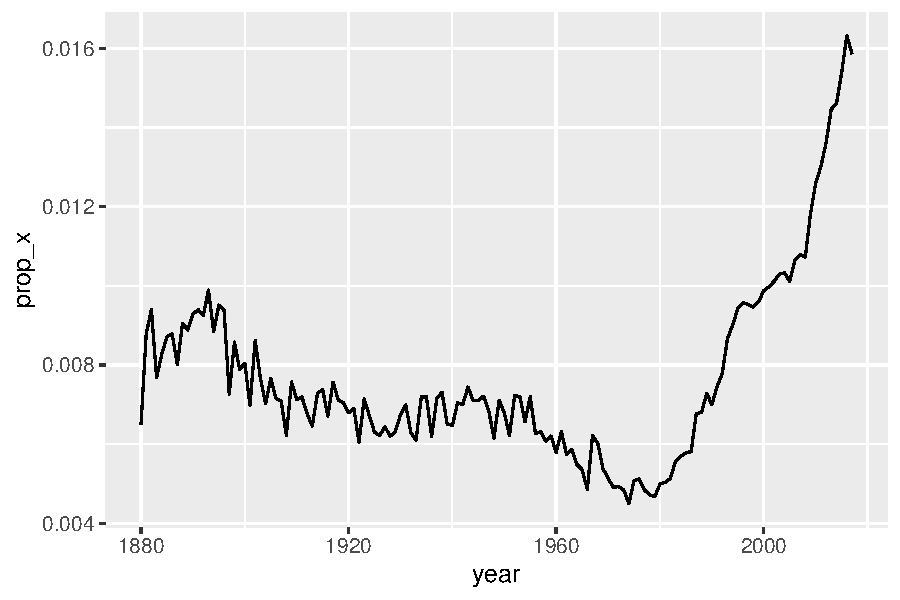
\includegraphics[width=18.75in,height=\textheight]{data-visualize_files/figure-pdf/unnamed-chunk-11-1.pdf}

当分类变量被映射到美学上时,ggplot2将自动为变量的每个水平(三个物种中的一个)分配一个唯一的美学值(这里是某种颜色),这个过程被称为\textbf{scaling}。g
gplot2还将添加一个图例,解释哪些值对应于哪些水平。

现在让我们再添加一层:一条显示体重和鳍长之间关系的平滑曲线。在
继续之前请参考上面的代码,并考虑如何将其添加到现有的图中。

由于这是一个代表数据的新geom,我们将在我们的点几何上添加一个新的geom作为图层:\texttt{geom\_smooth()}。我
们将指定基于\texttt{method\ =\ "lm"}的线性模型(\texttt{l}inear
\texttt{m}odel)绘制最佳拟合直线。

\begin{Shaded}
\begin{Highlighting}[]
\FunctionTok{ggplot}\NormalTok{(}
  \AttributeTok{data =}\NormalTok{ penguins,}
  \AttributeTok{mapping =} \FunctionTok{aes}\NormalTok{(}\AttributeTok{x =}\NormalTok{ flipper\_length\_mm, }\AttributeTok{y =}\NormalTok{ body\_mass\_g, }\AttributeTok{color =}\NormalTok{ species)}
\NormalTok{) }\SpecialCharTok{+}
  \FunctionTok{geom\_point}\NormalTok{() }\SpecialCharTok{+}
  \FunctionTok{geom\_smooth}\NormalTok{(}\AttributeTok{method =} \StringTok{"lm"}\NormalTok{)}
\end{Highlighting}
\end{Shaded}

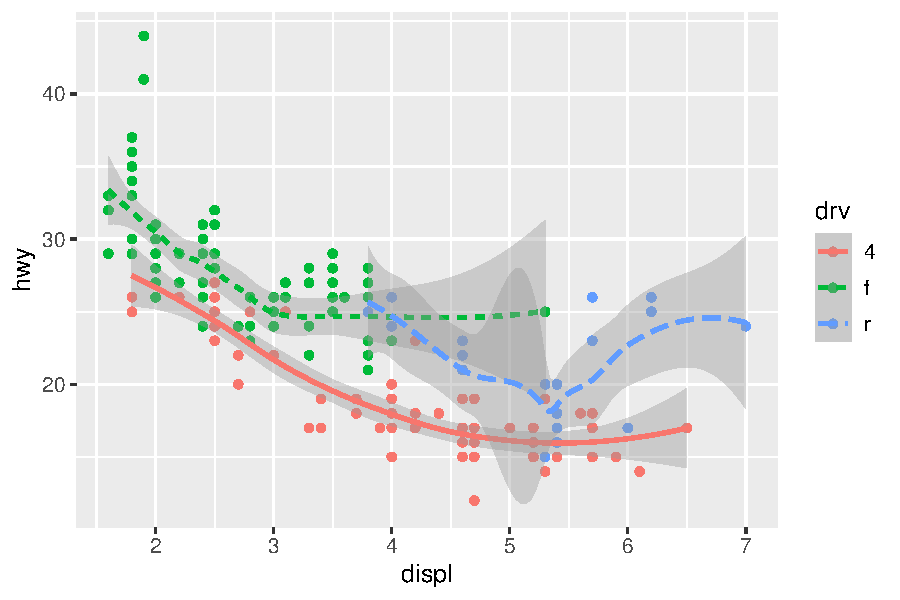
\includegraphics[width=18.75in,height=\textheight]{data-visualize_files/figure-pdf/unnamed-chunk-12-1.pdf}

我们已经成功地添加了直线,但是这个图和第 小节~\ref{sec-ultimate-goal}
节中的图看起来并不像,那里的图形整个数据集只有一条直线,而这里每个物种都有单独的一条直线。

在\texttt{ggplot()}中定义的美学映射(aesthetic
mappings)在全局级别时,会被传递到图的每一个后续的几何层(geom
layers)。然 而,ggplot2 中的每个geom函数也可以接受一个映射参数(mapping
argument),这允许在局部级别定义美学映射,这些映射会添加到从全局级别继承的映射中。由
于我们希望点(points)的颜色基于物种(species)来设置,但不想为它们将线(lines)分开,我们应该只在\texttt{geom\_point()}中指定\texttt{color\ =\ species}。

\begin{Shaded}
\begin{Highlighting}[]
\FunctionTok{ggplot}\NormalTok{(}
  \AttributeTok{data =}\NormalTok{ penguins,}
  \AttributeTok{mapping =} \FunctionTok{aes}\NormalTok{(}\AttributeTok{x =}\NormalTok{ flipper\_length\_mm, }\AttributeTok{y =}\NormalTok{ body\_mass\_g)}
\NormalTok{) }\SpecialCharTok{+}
  \FunctionTok{geom\_point}\NormalTok{(}\AttributeTok{mapping =} \FunctionTok{aes}\NormalTok{(}\AttributeTok{color =}\NormalTok{ species)) }\SpecialCharTok{+}
  \FunctionTok{geom\_smooth}\NormalTok{(}\AttributeTok{method =} \StringTok{"lm"}\NormalTok{)}
\end{Highlighting}
\end{Shaded}

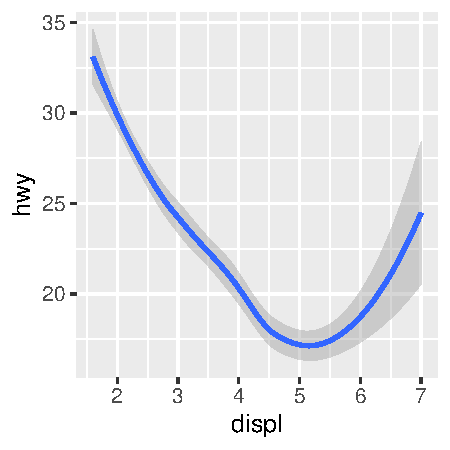
\includegraphics[width=18.75in,height=\textheight]{data-visualize_files/figure-pdf/unnamed-chunk-13-1.pdf}

瞧!我 们有了一些看起来很像我们最终目标的东西,尽管它还不完美。我
们仍然需要为每种企鹅使用不同的形状,并改进标签。

在图表上仅使用颜色来表示信息通常不是一个好主意,因为由于色盲或其他色觉差异,人们对颜色的感知会有所不同。因
此,除了颜色之外,我们还可以将\texttt{物种}映射到\texttt{形状}美学上。

\begin{Shaded}
\begin{Highlighting}[]
\FunctionTok{ggplot}\NormalTok{(}
  \AttributeTok{data =}\NormalTok{ penguins,}
  \AttributeTok{mapping =} \FunctionTok{aes}\NormalTok{(}\AttributeTok{x =}\NormalTok{ flipper\_length\_mm, }\AttributeTok{y =}\NormalTok{ body\_mass\_g)}
\NormalTok{) }\SpecialCharTok{+}
  \FunctionTok{geom\_point}\NormalTok{(}\AttributeTok{mapping =} \FunctionTok{aes}\NormalTok{(}\AttributeTok{color =}\NormalTok{ species, }\AttributeTok{shape =}\NormalTok{ species)) }\SpecialCharTok{+}
  \FunctionTok{geom\_smooth}\NormalTok{(}\AttributeTok{method =} \StringTok{"lm"}\NormalTok{)}
\end{Highlighting}
\end{Shaded}

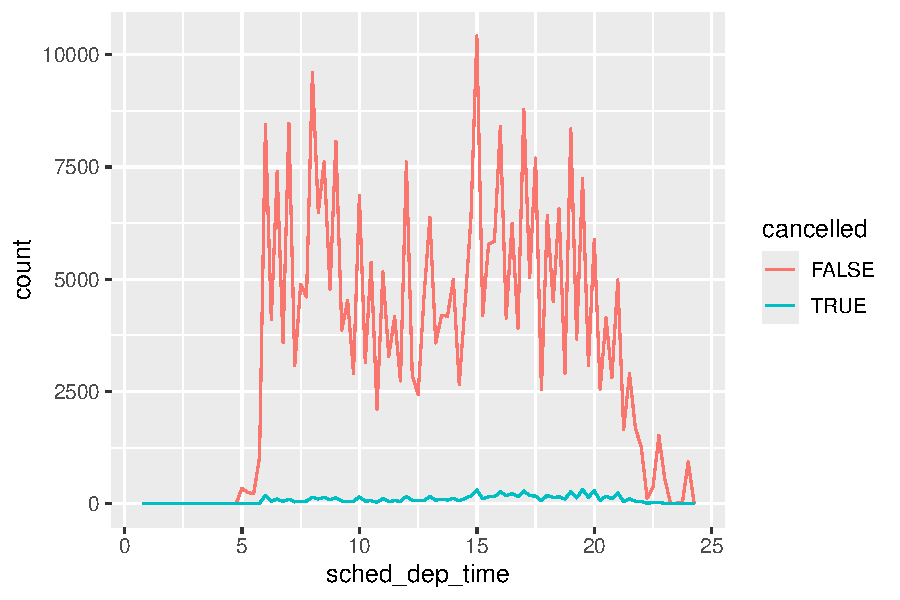
\includegraphics[width=18.75in,height=\textheight]{data-visualize_files/figure-pdf/unnamed-chunk-14-1.pdf}

注意,图例也会自动更新以反映点的不同形状。

最后,我们使用\texttt{labs()}函数在一个新的层中改进图的标签。\texttt{l}
\texttt{abs()}函数的一些参数含义是不言自明的:\texttt{title}用于添加标题,\texttt{subtitle}用于添加副标题。其
他参数与美学映射相对应,\texttt{x}是x轴的标签,\texttt{y}是y轴的标签,而\texttt{color}和\texttt{shape}则定义了图例中的标签。此
外,我们可以使用来自ggthemes包的\texttt{scale\_color\_colorblind()}函数来改进颜色调色板,以确保它对色盲用户也是安全的。

\begin{Shaded}
\begin{Highlighting}[]
\FunctionTok{ggplot}\NormalTok{(}
  \AttributeTok{data =}\NormalTok{ penguins,}
  \AttributeTok{mapping =} \FunctionTok{aes}\NormalTok{(}\AttributeTok{x =}\NormalTok{ flipper\_length\_mm, }\AttributeTok{y =}\NormalTok{ body\_mass\_g)}
\NormalTok{) }\SpecialCharTok{+}
  \FunctionTok{geom\_point}\NormalTok{(}\FunctionTok{aes}\NormalTok{(}\AttributeTok{color =}\NormalTok{ species, }\AttributeTok{shape =}\NormalTok{ species)) }\SpecialCharTok{+}
  \FunctionTok{geom\_smooth}\NormalTok{(}\AttributeTok{method =} \StringTok{"lm"}\NormalTok{) }\SpecialCharTok{+}
  \FunctionTok{labs}\NormalTok{(}
    \AttributeTok{title =} \StringTok{"Body mass and flipper length"}\NormalTok{,}
    \AttributeTok{subtitle =} \StringTok{"Dimensions for Adelie, Chinstrap, and Gentoo Penguins"}\NormalTok{,}
    \AttributeTok{x =} \StringTok{"Flipper length (mm)"}\NormalTok{, }\AttributeTok{y =} \StringTok{"Body mass (g)"}\NormalTok{,}
    \AttributeTok{color =} \StringTok{"Species"}\NormalTok{, }\AttributeTok{shape =} \StringTok{"Species"}
\NormalTok{  ) }\SpecialCharTok{+}
  \FunctionTok{scale\_color\_colorblind}\NormalTok{()}
\end{Highlighting}
\end{Shaded}

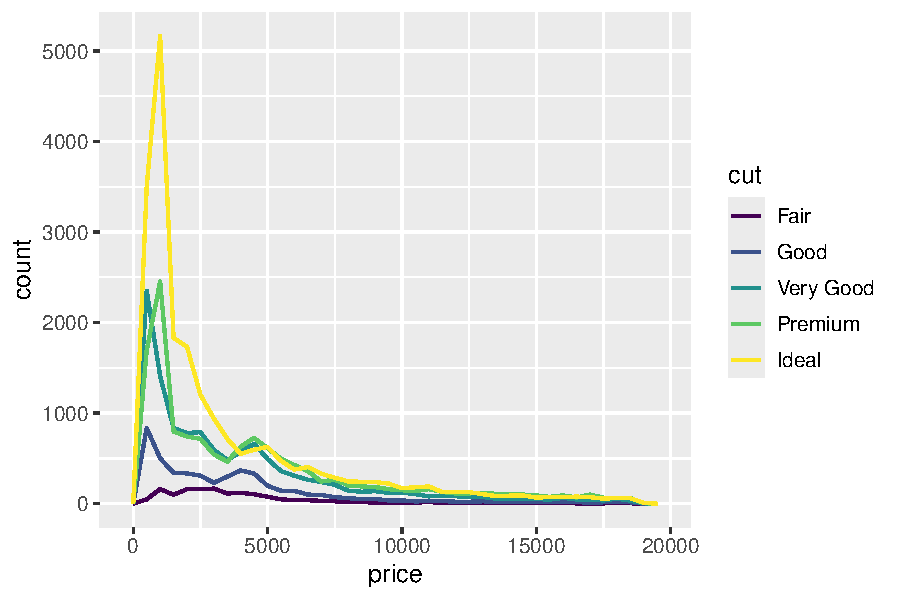
\includegraphics[width=18.75in,height=\textheight]{data-visualize_files/figure-pdf/unnamed-chunk-15-1.pdf}

我们终于有了一个完全符合我们``最终目标''的图形!

\subsection{练习}\label{ux7ec3ux4e60}

\begin{enumerate}
\def\labelenumi{\arabic{enumi}.}
\item
  \texttt{penguins}有多少行?多 少列?
\item
  数据框 \texttt{penguins} 中的 \texttt{bill\_depth\_mm}变量是什么?阅
  读 \texttt{?penguins} 的帮助文件后找到答案;
\item
  制作 \texttt{bill\_depth\_mm} 和 \texttt{bill\_length\_mm}
  的散点图;也就是说,创建一个散点图,y轴为\texttt{bill\_depth\_mm},
  x轴为\texttt{bill\_length\_mm}。描 述这两个变量之间的关系;
\item
  如果你做一个\texttt{species}与\texttt{bill\_depth\_mm}的散点图会发生什么?什
  么几何对象是更好的选择?
\item
  为什么下面的代码会给出一个错误,如何修复它?

\begin{Shaded}
\begin{Highlighting}[]
\FunctionTok{ggplot}\NormalTok{(}\AttributeTok{data =}\NormalTok{ penguins) }\SpecialCharTok{+} 
  \FunctionTok{geom\_point}\NormalTok{()}
\end{Highlighting}
\end{Shaded}
\item
  \texttt{na.rm}参数在\texttt{geom\_point()}中起什么作用?这
  个参数的默认值是什么?创
  建一个散点图,并在其中将这个参数设置为\texttt{TRUE}。
\item
  在你之前练习的图中添加以下标题:``数据来自 palmerpenguins 包。''
  提示:查看\texttt{labs()}函数的文档。
\item
  重新创建以下可视化。\texttt{b}
  \texttt{ill\_depth\_mm}应该映射到哪个美学属性上?它
  应该在全局级别映射还是在几何对象级别映射?

  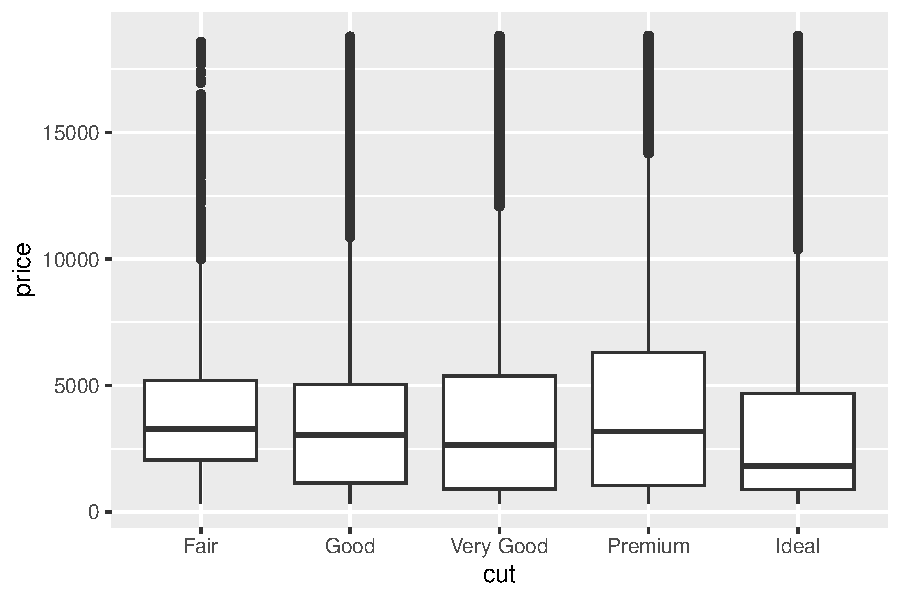
\includegraphics[width=18.75in,height=\textheight]{data-visualize_files/figure-pdf/unnamed-chunk-17-1.pdf}
\item
  在头脑中运行这段代码,预测输出将是什么样子;然后在R中运行代码并检查你的预测。

\begin{Shaded}
\begin{Highlighting}[]
\FunctionTok{ggplot}\NormalTok{(}
  \AttributeTok{data =}\NormalTok{ penguins,}
  \AttributeTok{mapping =} \FunctionTok{aes}\NormalTok{(}\AttributeTok{x =}\NormalTok{ flipper\_length\_mm, }\AttributeTok{y =}\NormalTok{ body\_mass\_g, }\AttributeTok{color =}\NormalTok{ island)}
\NormalTok{) }\SpecialCharTok{+}
  \FunctionTok{geom\_point}\NormalTok{() }\SpecialCharTok{+}
  \FunctionTok{geom\_smooth}\NormalTok{(}\AttributeTok{se =} \ConstantTok{FALSE}\NormalTok{)}
\end{Highlighting}
\end{Shaded}
\item
  这两张图看起来会不同吗?为 什么相同/为什么不同?

\begin{Shaded}
\begin{Highlighting}[]
\FunctionTok{ggplot}\NormalTok{(}
  \AttributeTok{data =}\NormalTok{ penguins,}
  \AttributeTok{mapping =} \FunctionTok{aes}\NormalTok{(}\AttributeTok{x =}\NormalTok{ flipper\_length\_mm, }\AttributeTok{y =}\NormalTok{ body\_mass\_g)}
\NormalTok{) }\SpecialCharTok{+}
  \FunctionTok{geom\_point}\NormalTok{() }\SpecialCharTok{+}
  \FunctionTok{geom\_smooth}\NormalTok{()}

\FunctionTok{ggplot}\NormalTok{() }\SpecialCharTok{+}
  \FunctionTok{geom\_point}\NormalTok{(}
    \AttributeTok{data =}\NormalTok{ penguins,}
    \AttributeTok{mapping =} \FunctionTok{aes}\NormalTok{(}\AttributeTok{x =}\NormalTok{ flipper\_length\_mm, }\AttributeTok{y =}\NormalTok{ body\_mass\_g)}
\NormalTok{  ) }\SpecialCharTok{+}
  \FunctionTok{geom\_smooth}\NormalTok{(}
    \AttributeTok{data =}\NormalTok{ penguins,}
    \AttributeTok{mapping =} \FunctionTok{aes}\NormalTok{(}\AttributeTok{x =}\NormalTok{ flipper\_length\_mm, }\AttributeTok{y =}\NormalTok{ body\_mass\_g)}
\NormalTok{  )}
\end{Highlighting}
\end{Shaded}
\end{enumerate}

\section{ggplot2 调用}\label{sec-ggplot2-calls}

随着从入门部分学习的深入,我们将过渡到更简洁的 ggplot2 代码表达式。到
目前为止,我们已经非常明确了,简化代码对你的学习是非常有帮助的:

\begin{Shaded}
\begin{Highlighting}[]
\FunctionTok{ggplot}\NormalTok{(}
  \AttributeTok{data =}\NormalTok{ penguins,}
  \AttributeTok{mapping =} \FunctionTok{aes}\NormalTok{(}\AttributeTok{x =}\NormalTok{ flipper\_length\_mm, }\AttributeTok{y =}\NormalTok{ body\_mass\_g)}
\NormalTok{) }\SpecialCharTok{+}
  \FunctionTok{geom\_point}\NormalTok{()}
\end{Highlighting}
\end{Shaded}

通常,函数的前一两个参数非常重要,你应该牢记它们。在
\texttt{ggplot()}中,前两个参数是\texttt{data}和\texttt{mapping},在本书的剩余部分,我们将不再提供这些参数的名称。这
样既节省打字时间,又可通过减少额外文字,更容易地看出不同图之间的差异。这
是一个非常重要的编程关注点,我们将在 章节~\ref{sec-functions}
中再次讨论。

将前面的图更简洁地重写为:

\begin{Shaded}
\begin{Highlighting}[]
\FunctionTok{ggplot}\NormalTok{(penguins, }\FunctionTok{aes}\NormalTok{(}\AttributeTok{x =}\NormalTok{ flipper\_length\_mm, }\AttributeTok{y =}\NormalTok{ body\_mass\_g)) }\SpecialCharTok{+} 
  \FunctionTok{geom\_point}\NormalTok{()}
\end{Highlighting}
\end{Shaded}

在将来,您还将了解管道\texttt{\textbar{}\textgreater{}},它将允许你使用以下命令创建该图形:

\begin{Shaded}
\begin{Highlighting}[]
\NormalTok{penguins }\SpecialCharTok{|\textgreater{}} 
  \FunctionTok{ggplot}\NormalTok{(}\FunctionTok{aes}\NormalTok{(}\AttributeTok{x =}\NormalTok{ flipper\_length\_mm, }\AttributeTok{y =}\NormalTok{ body\_mass\_g)) }\SpecialCharTok{+} 
  \FunctionTok{geom\_point}\NormalTok{()}
\end{Highlighting}
\end{Shaded}

\section{可视化分布}\label{ux53efux89c6ux5316ux5206ux5e03}

如何可视化变量的分布取决于变量的类型:分类还是数值。

\subsection{分类变量}\label{ux5206ux7c7bux53d8ux91cf}

如果一个变量只能取一小组值中的一个,那么它就是分类变量。要
检查分类变量的分布,可以使用条形图。条
形图的高度显示了每个\texttt{x}值的观测次数。

\begin{Shaded}
\begin{Highlighting}[]
\FunctionTok{ggplot}\NormalTok{(penguins, }\FunctionTok{aes}\NormalTok{(}\AttributeTok{x =}\NormalTok{ species)) }\SpecialCharTok{+}
  \FunctionTok{geom\_bar}\NormalTok{()}
\end{Highlighting}
\end{Shaded}

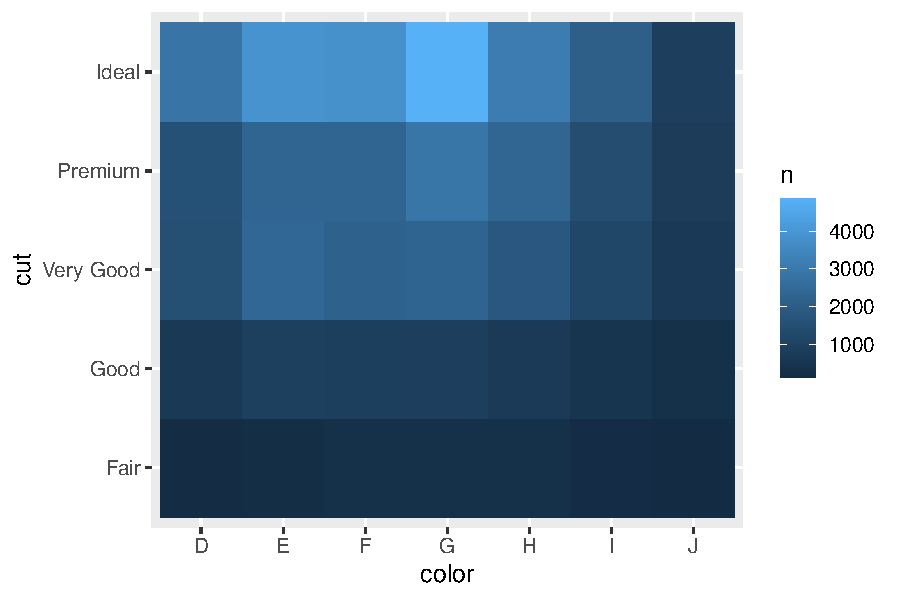
\includegraphics[width=18.75in,height=\textheight]{data-visualize_files/figure-pdf/unnamed-chunk-23-1.pdf}

在具有非有序水平的分类变量的条形图中,如上面提到的企鹅\textbf{物种},通常更可取思路的是根据它们的频率重新排序条形图。这
样做需要将变量转换为因子(R如何处理分类数据),然后重新排序该因子的水平。

\begin{Shaded}
\begin{Highlighting}[]
\FunctionTok{ggplot}\NormalTok{(penguins, }\FunctionTok{aes}\NormalTok{(}\AttributeTok{x =} \FunctionTok{fct\_infreq}\NormalTok{(species))) }\SpecialCharTok{+}
  \FunctionTok{geom\_bar}\NormalTok{()}
\end{Highlighting}
\end{Shaded}

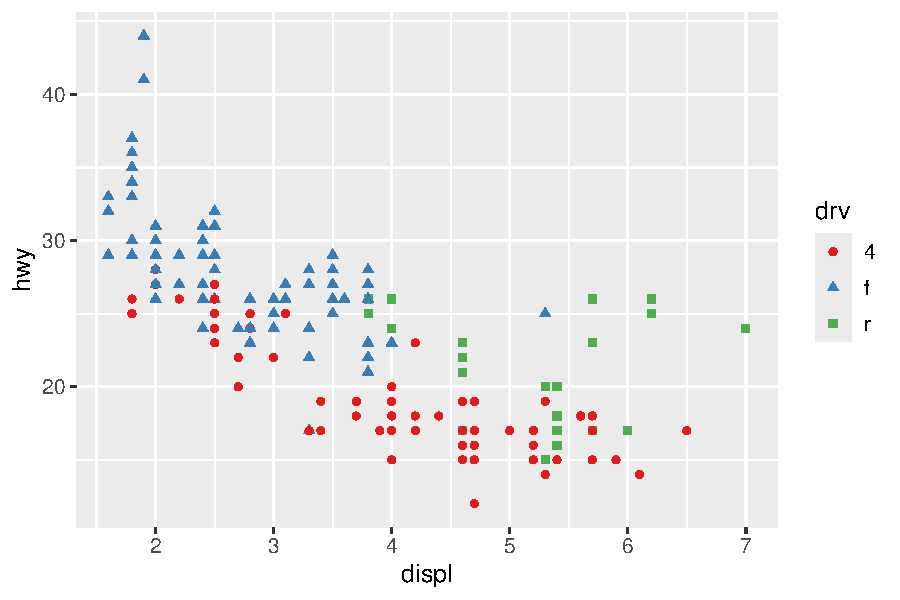
\includegraphics[width=18.75in,height=\textheight]{data-visualize_files/figure-pdf/unnamed-chunk-24-1.pdf}

您将在@sec-factors
中学到更多关于因子和处理因子的函数(如上面用到的\texttt{fct\_infreq()})。

\subsection{数值变量}\label{ux6570ux503cux53d8ux91cf}

如果一个变量可以在一个大的数值范围内取值,并且对这些数值进行加、减或取平均数是有意义的,那么这个变量就是数值型(或定量型)的。数
值型变量可以是连续的,也可以是离散的。

一个常用于连续变量分布的可视化方法是直方图。

\begin{Shaded}
\begin{Highlighting}[]
\FunctionTok{ggplot}\NormalTok{(penguins, }\FunctionTok{aes}\NormalTok{(}\AttributeTok{x =}\NormalTok{ body\_mass\_g)) }\SpecialCharTok{+}
  \FunctionTok{geom\_histogram}\NormalTok{(}\AttributeTok{binwidth =} \DecValTok{200}\NormalTok{)}
\end{Highlighting}
\end{Shaded}

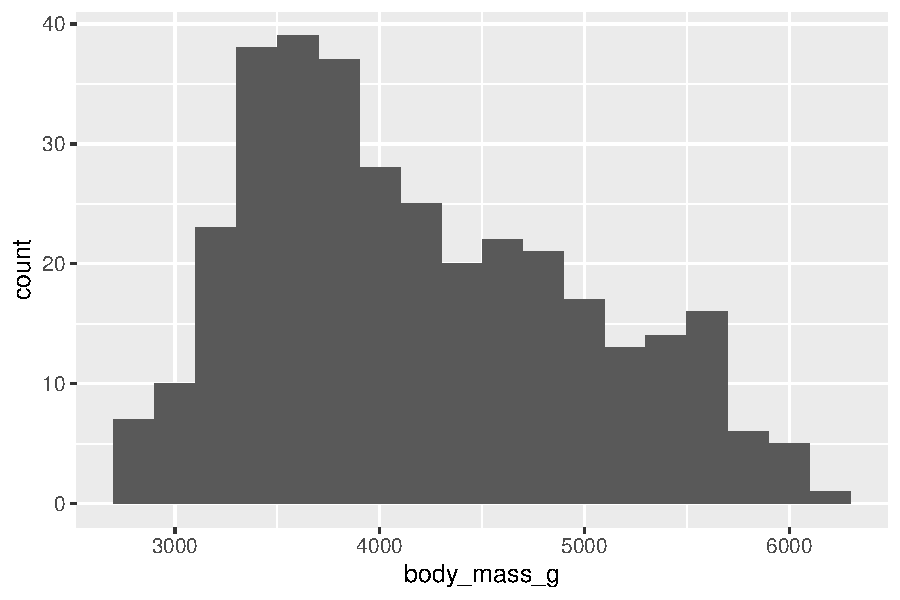
\includegraphics[width=18.75in,height=\textheight]{data-visualize_files/figure-pdf/unnamed-chunk-25-1.pdf}

直方图将x轴分成等间距的区间(或称为``箱''),然后使用条形的高度来显示落在每个区间内的观察值的数量。在
上面的图中,最高的条形表示有39个观察值的\texttt{body\_mass\_g}值在3,500克到3,700克之间,这是条形的左右边缘。

你可以使用binwidth参数来设置直方图中区间的宽度,这个参数是以\texttt{x}变量的单位来衡量的。当
使用直方图时,你应该探索不同的区间宽度,因为不同的区间宽度可能会揭示不同的模式。在
下面的图中,区间宽度为20太窄了,导致条形太多,使得难以确定分布的形状。类
似地,区间宽度为2,000太高了,导致所有数据只被分到三个条形中,也难以确定分布的形状。区
间宽度取200达到了合理的平衡。

\begin{Shaded}
\begin{Highlighting}[]
\FunctionTok{ggplot}\NormalTok{(penguins, }\FunctionTok{aes}\NormalTok{(}\AttributeTok{x =}\NormalTok{ body\_mass\_g)) }\SpecialCharTok{+}
  \FunctionTok{geom\_histogram}\NormalTok{(}\AttributeTok{binwidth =} \DecValTok{20}\NormalTok{)}
\FunctionTok{ggplot}\NormalTok{(penguins, }\FunctionTok{aes}\NormalTok{(}\AttributeTok{x =}\NormalTok{ body\_mass\_g)) }\SpecialCharTok{+}
  \FunctionTok{geom\_histogram}\NormalTok{(}\AttributeTok{binwidth =} \DecValTok{2000}\NormalTok{)}
\end{Highlighting}
\end{Shaded}

\begin{figure}

\begin{minipage}{0.50\linewidth}
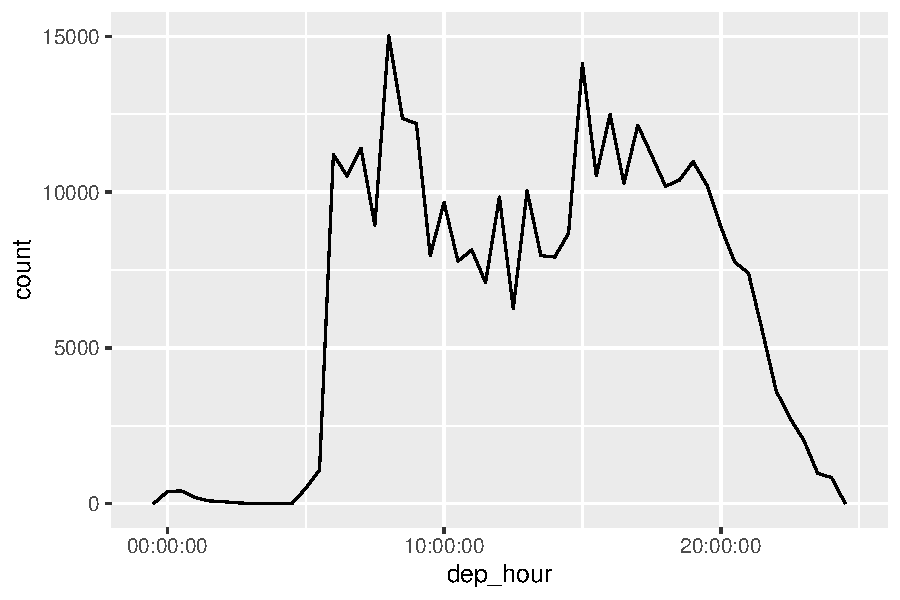
\includegraphics[width=9.375in,height=\textheight]{data-visualize_files/figure-pdf/unnamed-chunk-26-1.pdf}\end{minipage}%
%
\begin{minipage}{0.50\linewidth}
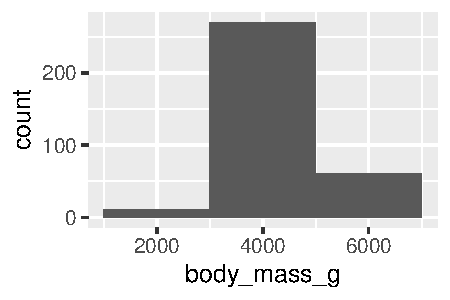
\includegraphics[width=9.375in,height=\textheight]{data-visualize_files/figure-pdf/unnamed-chunk-26-2.pdf}\end{minipage}%

\end{figure}%

数值变量分布的另一种可视化方式是密度图。密
度图是直方图的平滑版本,是连续数据的实用替代方案,特别是当数据来自一个潜在的平滑分布时。我
们不会深入了解\texttt{geom\_density()}如何估计密度(你可以在函数文档中了解更多),但我们可通过一个类比来解释如何绘制密度曲线。想
象一个由木块制成的直方图,然后想象你在直方图上放下一根煮熟的面条,面条在木块上披挂的形状可以看作是密度曲线的形状。与
直方图相比,它显示的细节较少,但可以更容易地快速了解分布的形状,特别是关于众数和偏态。

\begin{Shaded}
\begin{Highlighting}[]
\FunctionTok{ggplot}\NormalTok{(penguins, }\FunctionTok{aes}\NormalTok{(}\AttributeTok{x =}\NormalTok{ body\_mass\_g)) }\SpecialCharTok{+}
  \FunctionTok{geom\_density}\NormalTok{()}
\CommentTok{\#\textgreater{} Warning: Removed 2 rows containing non{-}finite outside the scale range}
\CommentTok{\#\textgreater{} (\textasciigrave{}stat\_density()\textasciigrave{}).}
\end{Highlighting}
\end{Shaded}

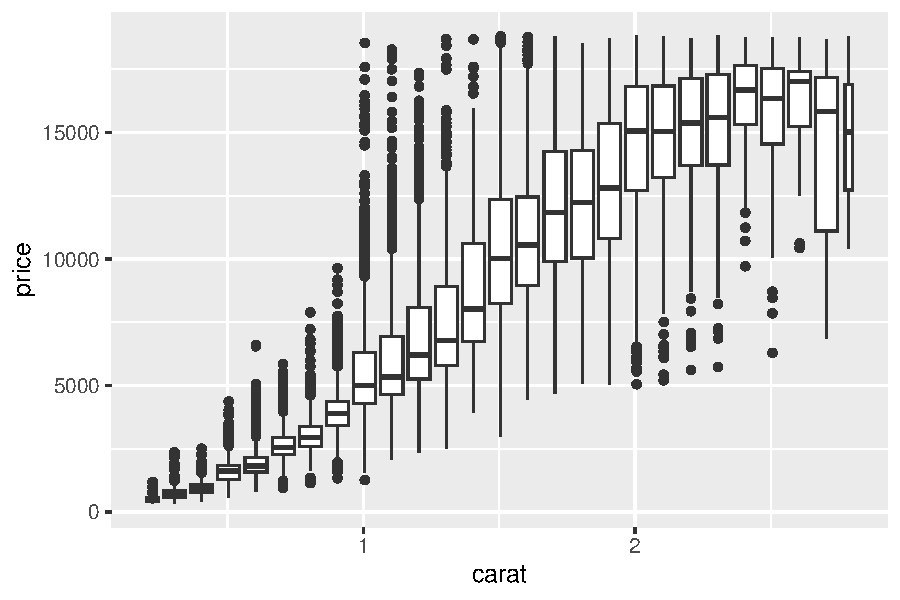
\includegraphics[width=18.75in,height=\textheight]{data-visualize_files/figure-pdf/unnamed-chunk-27-1.pdf}

\subsection{练习}\label{ux7ec3ux4e60-1}

\begin{enumerate}
\def\labelenumi{\arabic{enumi}.}
\item
  做一个企鹅种类的条形图,把物种分配给\texttt{y}。这 个图有什么不同?
\item
  下面两个图有什么不同?哪 种美学(颜色或填充)对改变条的颜色更有用?

\begin{Shaded}
\begin{Highlighting}[]
\FunctionTok{ggplot}\NormalTok{(penguins, }\FunctionTok{aes}\NormalTok{(}\AttributeTok{x =}\NormalTok{ species)) }\SpecialCharTok{+}
  \FunctionTok{geom\_bar}\NormalTok{(}\AttributeTok{color =} \StringTok{"red"}\NormalTok{)}

\FunctionTok{ggplot}\NormalTok{(penguins, }\FunctionTok{aes}\NormalTok{(}\AttributeTok{x =}\NormalTok{ species)) }\SpecialCharTok{+}
  \FunctionTok{geom\_bar}\NormalTok{(}\AttributeTok{fill =} \StringTok{"red"}\NormalTok{)}
\end{Highlighting}
\end{Shaded}
\item
  \texttt{geom\_histogram()} 中的参数 \texttt{bins} 起什么作用?
\item
  在加载tidyverse包后,对\texttt{diamonds}数据集中的\texttt{carat}变量制作一个直方图。尝
  试使用不同的区间宽度。哪 种区间宽度揭示了最有趣的模式?
\end{enumerate}

\section{可视化关系}\label{ux53efux89c6ux5316ux5173ux7cfb}

为了可视化关系,我们需要将至少两个变量映射到图的美学上。在
下面的内容中,你将了解用于可视化两个或多个变量之间关系的常用绘图以及用于创建它们的几何图形。

To visualize a relationship we need to have at least two variables
mapped to aesthetics of a plot. In the following sections you will learn
about commonly used plots for visualizing relationships between two or
more variables and the geoms used for creating them.

\subsection{数值变量和分类变量}\label{ux6570ux503cux53d8ux91cfux548cux5206ux7c7bux53d8ux91cf}

为了可视化数值变量和分类变量之间的关系,我们可以使用并列箱线图。\textbf{箱}
\textbf{线图}是一种描述分布的位置度量指标(百分位数)的视觉简写形式,它还有助于识别潜在的异常值。如
图~\ref{fig-eda-boxplot} 所示,每个箱线图包括:

\begin{itemize}
\tightlist
\item
  一个箱子,表示数据中间一半的范围,即从分布的25\%百分位数到75\%百分位数的距离,这个距离称为四分位距(\textbf{i}nter\textbf{q}uartile
  \textbf{r}ange,IQR)。在箱子的中间有一条线,表示分布的中位数,即50\%百分位数。这三条线可以让你感受到分布的离散程度以及分布是否关于中位数对称或偏向一侧。
\item
  视觉点,用于显示距离箱子边缘超过1.5倍IQR的观测值。这些异常点是不寻常的,因此单独绘制。
\item
  一条线(或称为``胡须''),从箱子的每个末端延伸出去,直到分布中最远的非异常值点。
\end{itemize}

\begin{figure}

\centering{

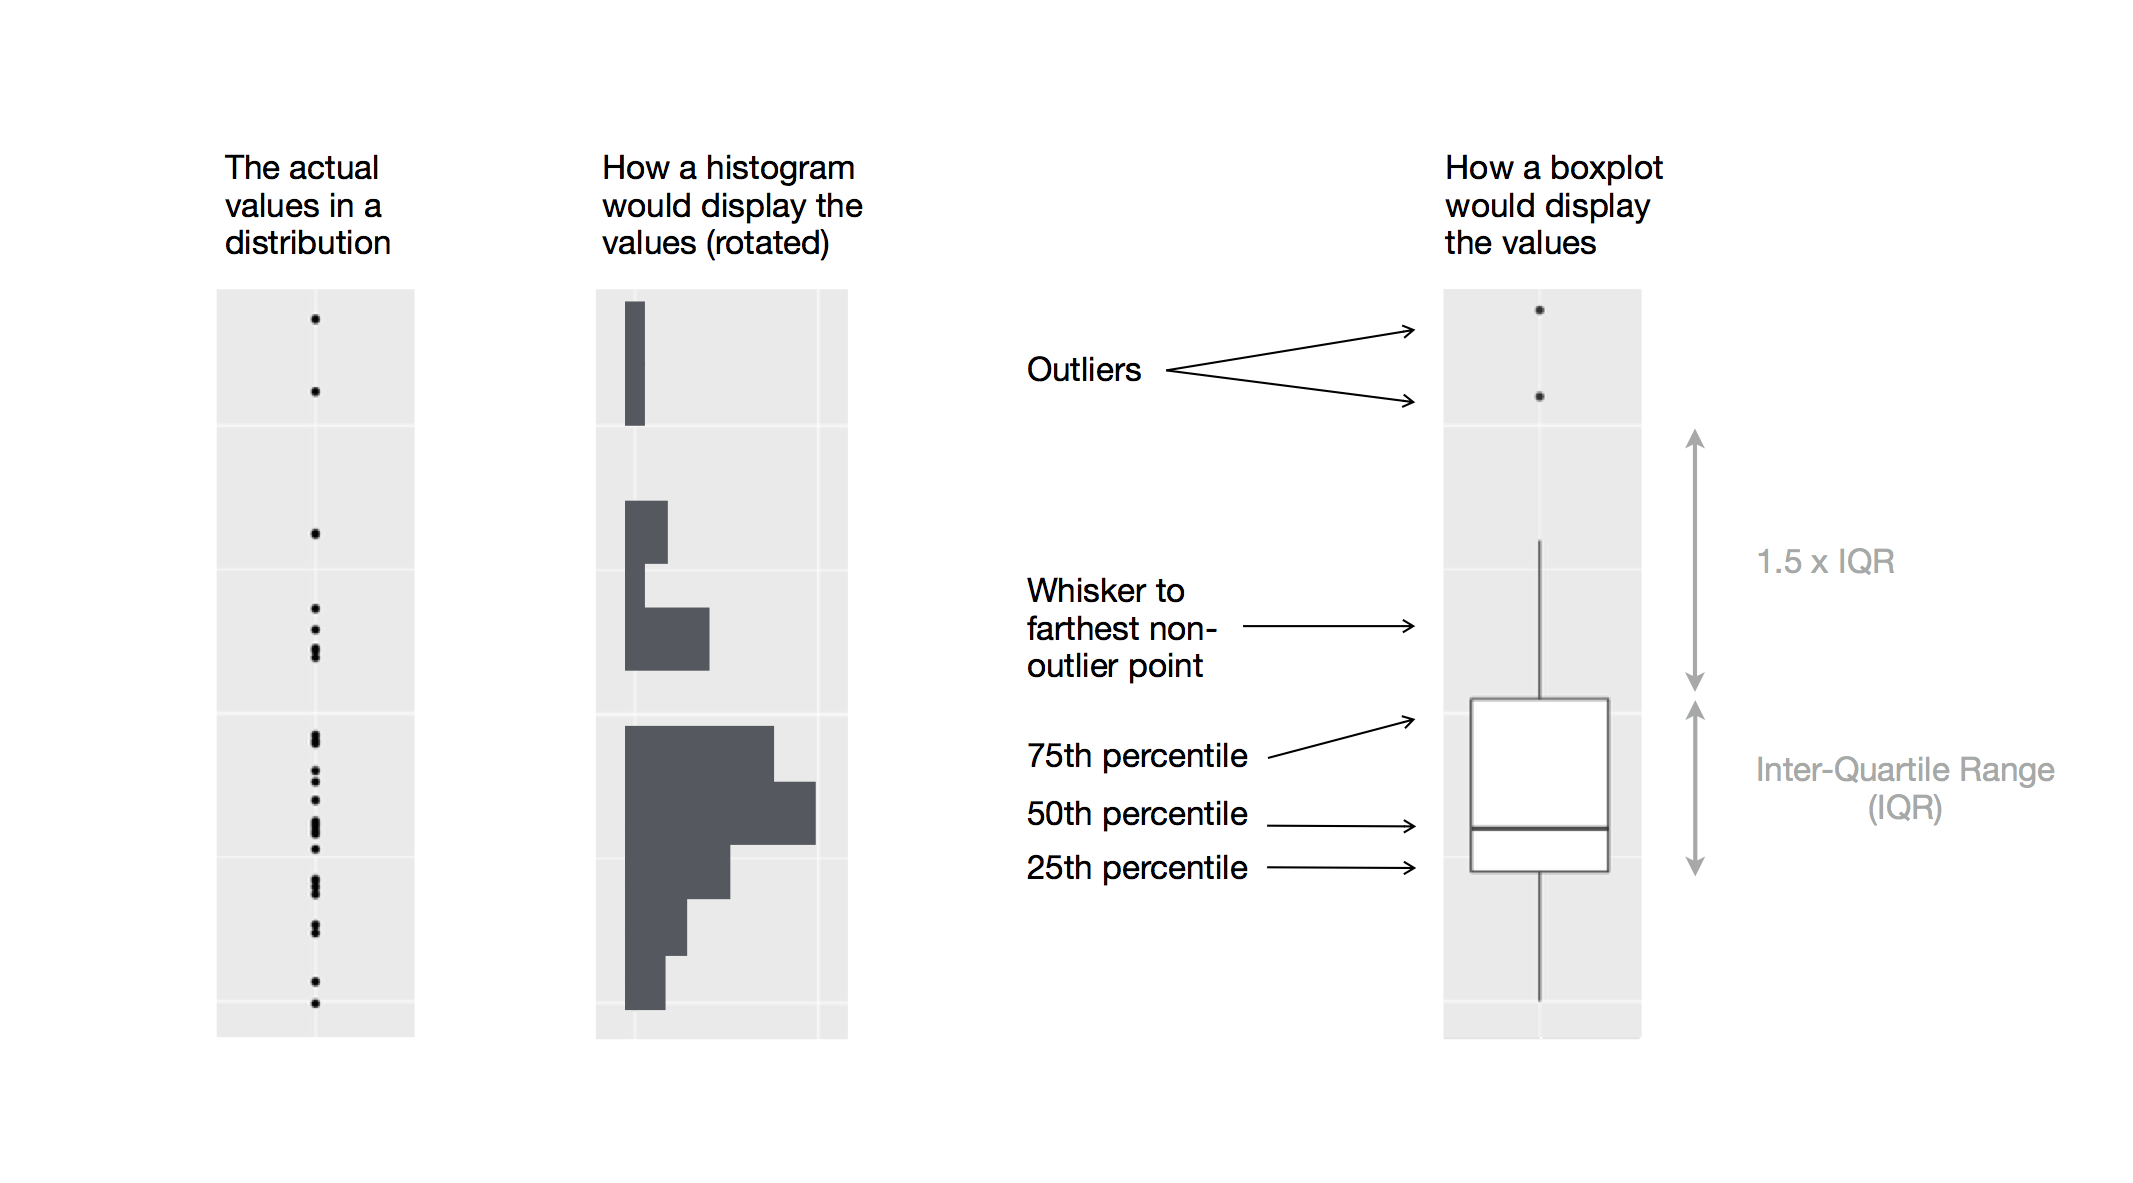
\includegraphics[width=3.56in,height=\textheight]{images/EDA-boxplot.png}

}

\caption{\label{fig-eda-boxplot}Diagram depicting how a boxplot is
created.}

\end{figure}%

让我们用\texttt{geom\_boxplot()}来看看按物种分组的企鹅体重的分布:

\begin{Shaded}
\begin{Highlighting}[]
\FunctionTok{ggplot}\NormalTok{(penguins, }\FunctionTok{aes}\NormalTok{(}\AttributeTok{x =}\NormalTok{ species, }\AttributeTok{y =}\NormalTok{ body\_mass\_g)) }\SpecialCharTok{+}
  \FunctionTok{geom\_boxplot}\NormalTok{()}
\end{Highlighting}
\end{Shaded}

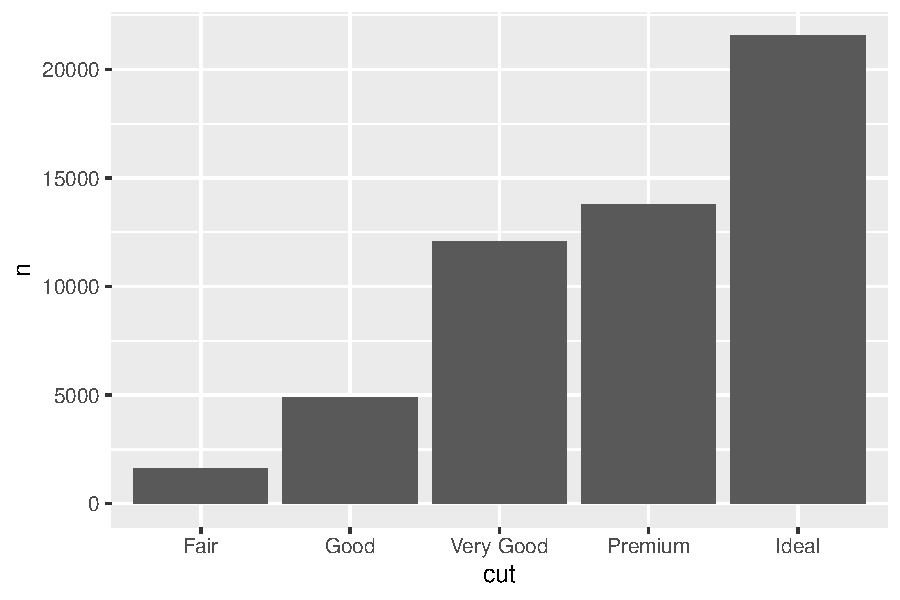
\includegraphics[width=18.75in,height=\textheight]{data-visualize_files/figure-pdf/unnamed-chunk-30-1.pdf}

或者,使用\texttt{geom\_density()}绘制密度图。

\begin{Shaded}
\begin{Highlighting}[]
\FunctionTok{ggplot}\NormalTok{(penguins, }\FunctionTok{aes}\NormalTok{(}\AttributeTok{x =}\NormalTok{ body\_mass\_g, }\AttributeTok{color =}\NormalTok{ species)) }\SpecialCharTok{+}
  \FunctionTok{geom\_density}\NormalTok{(}\AttributeTok{linewidth =} \FloatTok{0.75}\NormalTok{)}
\end{Highlighting}
\end{Shaded}

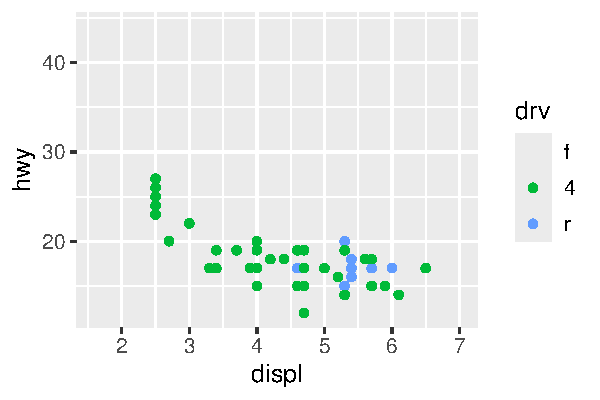
\includegraphics[width=18.75in,height=\textheight]{data-visualize_files/figure-pdf/unnamed-chunk-31-1.pdf}

我们还使用了\texttt{linewidth}参数来定制线条的粗细,以便使它们在背景中更加突出。

此外,我们可以将物种映射到颜色和填充的美学特性,并使用\texttt{alpha}美学特性为填充的密度曲线添加透明度。这
个美学特性取值范围在0(完全透明)和1(完全不透明)之间。在
下图中,它被设置为0.5。

\begin{Shaded}
\begin{Highlighting}[]
\FunctionTok{ggplot}\NormalTok{(penguins, }\FunctionTok{aes}\NormalTok{(}\AttributeTok{x =}\NormalTok{ body\_mass\_g, }\AttributeTok{color =}\NormalTok{ species, }\AttributeTok{fill =}\NormalTok{ species)) }\SpecialCharTok{+}
  \FunctionTok{geom\_density}\NormalTok{(}\AttributeTok{alpha =} \FloatTok{0.5}\NormalTok{)}
\end{Highlighting}
\end{Shaded}

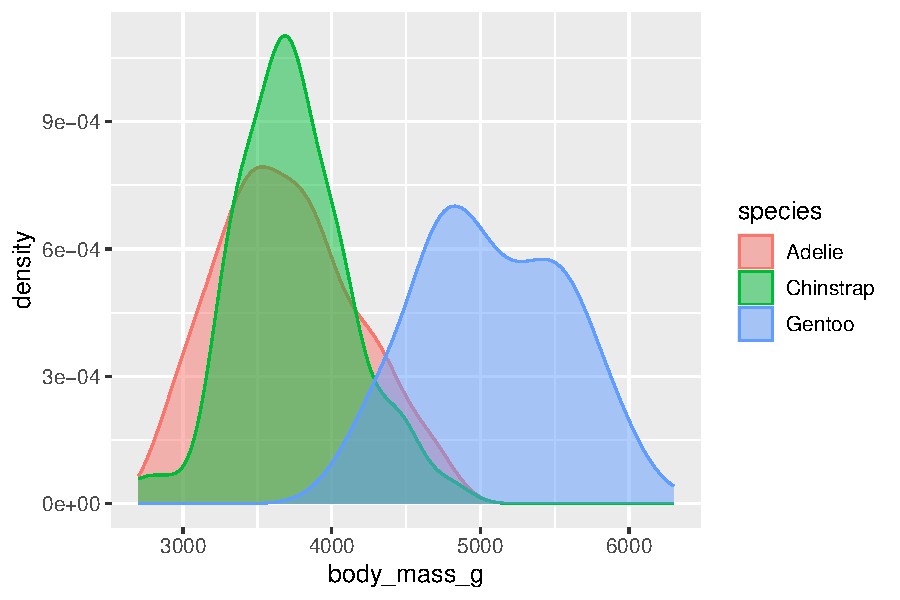
\includegraphics[width=18.75in,height=\textheight]{data-visualize_files/figure-pdf/unnamed-chunk-32-1.pdf}

注意我们在这里使用的术语:

\begin{itemize}
\tightlist
\item
  如果想让美学所代表的视觉属性根据变量的值而变化,我们可以将变量映射到美学。
\item
  否则,设置该美学特性的值。
\end{itemize}

\subsection{两个分类变量}\label{ux4e24ux4e2aux5206ux7c7bux53d8ux91cf}

我们可以使用堆叠条形图来可视化两个分类变量之间的关系。例
如,下面的两个堆叠条形图都显示了\texttt{岛屿}和\texttt{物种}之间的关系,或者具体地说,显示了每个岛屿内物种的分布。

第一张图显示了每个岛屿上每种企鹅的频数。频
数图显示,每个岛上的Adelies企鹅数量相等。但
是,我们无法很好地感知每个岛屿内部的比例平衡。

\begin{Shaded}
\begin{Highlighting}[]
\FunctionTok{ggplot}\NormalTok{(penguins, }\FunctionTok{aes}\NormalTok{(}\AttributeTok{x =}\NormalTok{ island, }\AttributeTok{fill =}\NormalTok{ species)) }\SpecialCharTok{+}
  \FunctionTok{geom\_bar}\NormalTok{()}
\end{Highlighting}
\end{Shaded}

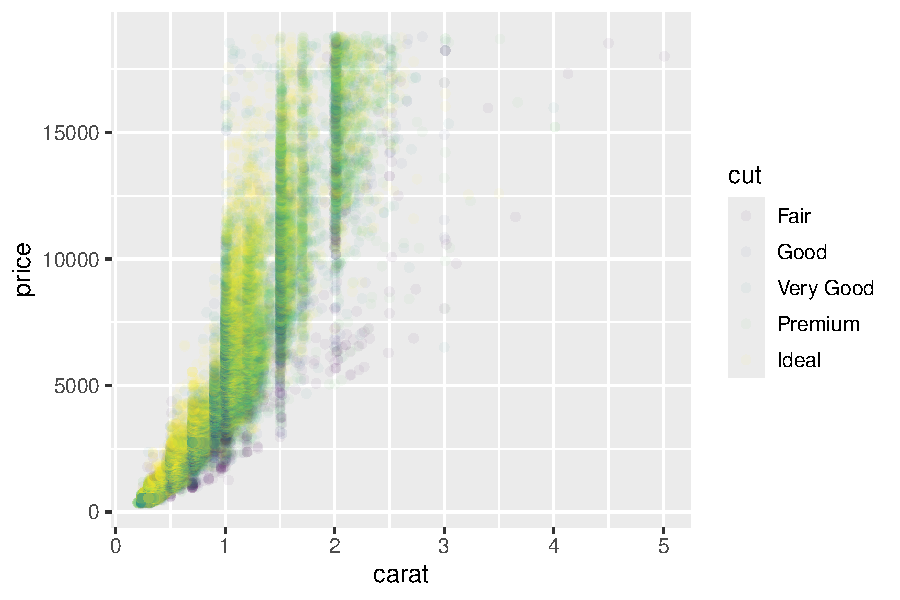
\includegraphics[width=18.75in,height=\textheight]{data-visualize_files/figure-pdf/unnamed-chunk-33-1.pdf}

第二个图是通过在geom中设置\texttt{position\ =\ "fill"}创建的相对频数图,它对于比较不同岛屿上的物种分布更有用,因为它不受岛屿之间企鹅数量不等的影响。根
据此图,我们可以看到Gentoo企鹅都生活在Biscoe岛上,约占该岛屿企鹅的75\%,Chinstrap企鹅都生活在Dream岛上,约占该岛屿企鹅的50\%,而Adelie企鹅生活在所有三个岛屿上,并且Torgersen岛上都是Torgersen企鹅。

\begin{Shaded}
\begin{Highlighting}[]
\FunctionTok{ggplot}\NormalTok{(penguins, }\FunctionTok{aes}\NormalTok{(}\AttributeTok{x =}\NormalTok{ island, }\AttributeTok{fill =}\NormalTok{ species)) }\SpecialCharTok{+}
  \FunctionTok{geom\_bar}\NormalTok{(}\AttributeTok{position =} \StringTok{"fill"}\NormalTok{)}
\end{Highlighting}
\end{Shaded}

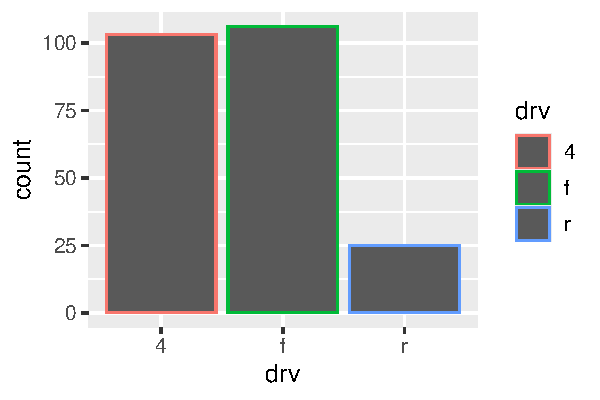
\includegraphics[width=18.75in,height=\textheight]{data-visualize_files/figure-pdf/unnamed-chunk-34-1.pdf}

在创建这些条形图时,我们将要被分割成条形的变量映射到\texttt{x}美学上,而将改变条形内部颜色的变量映射到\texttt{fill}美学上。

\subsection{两个数值变量}\label{ux4e24ux4e2aux6570ux503cux53d8ux91cf}

到目前为止,你已经学习了散点图(用\texttt{geom\_point()}创建)和平滑曲线(用\texttt{geom\_smooth()}创建),用于可视化两个数值变量之间的关系。散
点图可能是用于可视化两个数值变量间关系的最常用图形。

\begin{Shaded}
\begin{Highlighting}[]
\FunctionTok{ggplot}\NormalTok{(penguins, }\FunctionTok{aes}\NormalTok{(}\AttributeTok{x =}\NormalTok{ flipper\_length\_mm, }\AttributeTok{y =}\NormalTok{ body\_mass\_g)) }\SpecialCharTok{+}
  \FunctionTok{geom\_point}\NormalTok{()}
\end{Highlighting}
\end{Shaded}

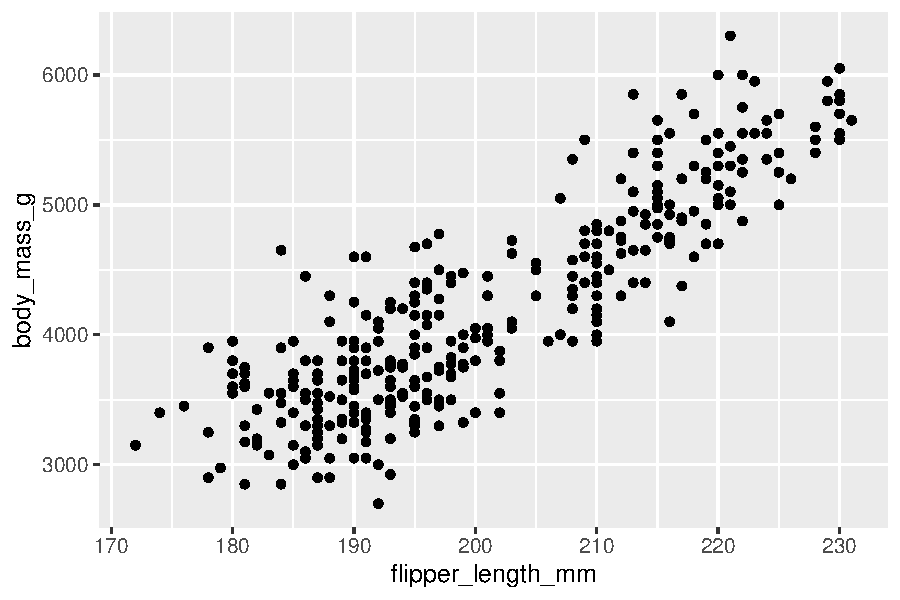
\includegraphics[width=18.75in,height=\textheight]{data-visualize_files/figure-pdf/unnamed-chunk-35-1.pdf}

\subsection{三个或更多变量}\label{ux4e09ux4e2aux6216ux66f4ux591aux53d8ux91cf}

正如我们在@sec-adding-aesthetics-layers
中看到的,我们可以通过将更多变量映射到额外的美学特性来将它们融入图表中。例
如,在下面的散点图中,点的颜色代表物种,而点的形状代表岛屿。

\begin{Shaded}
\begin{Highlighting}[]
\FunctionTok{ggplot}\NormalTok{(penguins, }\FunctionTok{aes}\NormalTok{(}\AttributeTok{x =}\NormalTok{ flipper\_length\_mm, }\AttributeTok{y =}\NormalTok{ body\_mass\_g)) }\SpecialCharTok{+}
  \FunctionTok{geom\_point}\NormalTok{(}\FunctionTok{aes}\NormalTok{(}\AttributeTok{color =}\NormalTok{ species, }\AttributeTok{shape =}\NormalTok{ island))}
\end{Highlighting}
\end{Shaded}

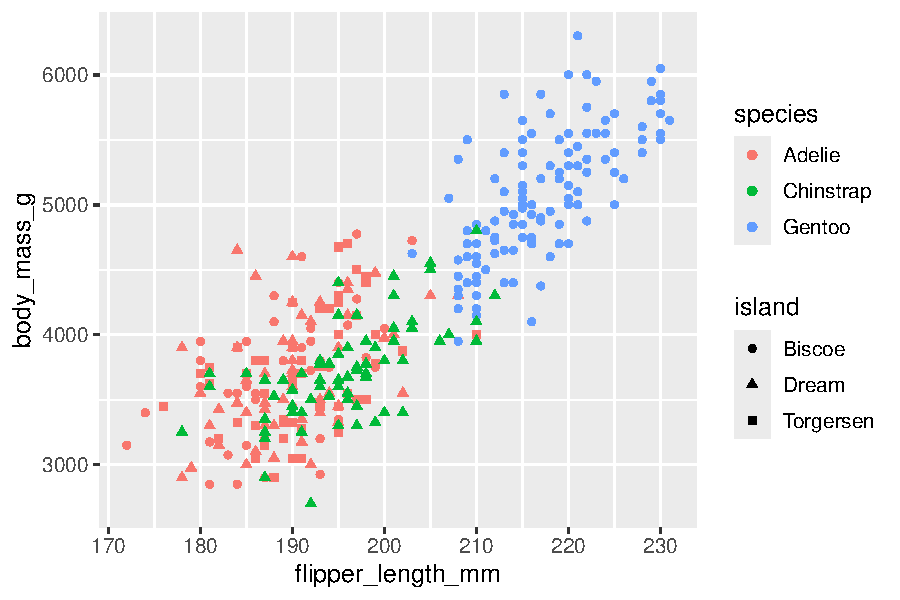
\includegraphics[width=18.75in,height=\textheight]{data-visualize_files/figure-pdf/unnamed-chunk-36-1.pdf}

然而,在图表中添加过多的美学映射会使它变得杂乱无章且难以理解。另
一种特别适用于分类变量的方法是将图形拆分为多个分面(\textbf{facets}),即每个分面显示数据的一个子集。

要通过单个变量将图表拆分为分面,请使用\texttt{facet\_wrap()}。\texttt{f}
\texttt{acet\_wrap()}的第一个参数是一个公式(formula)\footnote{这里的``formula''是由\textasciitilde 创建的事物的名称,而不是``equation''的同义词。},通过\texttt{\textasciitilde{}}后跟变量名来创建这个公式,传递给\texttt{facet\_wrap()}的变量应该是分类变量。

\begin{Shaded}
\begin{Highlighting}[]
\FunctionTok{ggplot}\NormalTok{(penguins, }\FunctionTok{aes}\NormalTok{(}\AttributeTok{x =}\NormalTok{ flipper\_length\_mm, }\AttributeTok{y =}\NormalTok{ body\_mass\_g)) }\SpecialCharTok{+}
  \FunctionTok{geom\_point}\NormalTok{(}\FunctionTok{aes}\NormalTok{(}\AttributeTok{color =}\NormalTok{ species, }\AttributeTok{shape =}\NormalTok{ species)) }\SpecialCharTok{+}
  \FunctionTok{facet\_wrap}\NormalTok{(}\SpecialCharTok{\textasciitilde{}}\NormalTok{island)}
\end{Highlighting}
\end{Shaded}

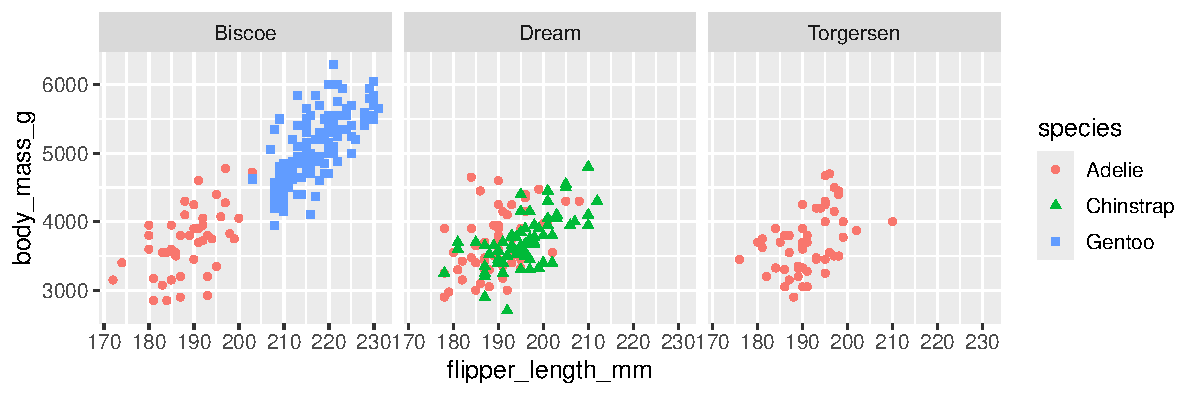
\includegraphics[width=25in,height=\textheight]{data-visualize_files/figure-pdf/unnamed-chunk-37-1.pdf}

在@sec-layers
中,你将学习许多其他用于可视化变量分布以及它们之间关系的几何对象(geoms)。

\subsection{练习}\label{ux7ec3ux4e60-2}

\begin{enumerate}
\def\labelenumi{\arabic{enumi}.}
\item
  \texttt{ggplot2}包中捆绑的\texttt{mpg}数据框包含了美国环境保护局收集的234个观测值,涵盖了38种汽车型号。\texttt{m}
  \texttt{pg}中的哪些变量是分类变量?哪 些变量是数值变量?(
  提示:键入\texttt{?mpg}以读取数据集的文档。)当你运行\texttt{mpg}时,如何查看这些信息?
\item
  使用\texttt{mpg}数据框制作\texttt{hwy}与\texttt{displ}的散点图。接
  下来,将第三个数值变量映射到
  \texttt{color},然后映射到\texttt{size},再同时映射到\texttt{color}和\texttt{size},最后映射到\texttt{shape}。这
  些美学特性在分类变量与数值变量上表现有何不同?
\item
  在\texttt{hwy}与\texttt{displ}的散点图中,如果将第三个变量映射到\texttt{linewidth},会发生什么?
\item
  如果你将同一个变量映射到多个美学特性上会发生什么?
\item
  制作\texttt{bill\_depth\_mm}与\texttt{bill\_length\_mm}的散点图,并按\texttt{species}对点进行着色。通
  过按物种着色,可以揭示这两个变量之间的关系是什么?如
  果按\texttt{species}分面又会如何?
\item
  为什么以下代码会生成两个独立的图例?你 如何修复它以合并这两个图例?

\begin{Shaded}
\begin{Highlighting}[]
\FunctionTok{ggplot}\NormalTok{(}
  \AttributeTok{data =}\NormalTok{ penguins,}
  \AttributeTok{mapping =} \FunctionTok{aes}\NormalTok{(}
    \AttributeTok{x =}\NormalTok{ bill\_length\_mm, }\AttributeTok{y =}\NormalTok{ bill\_depth\_mm, }
    \AttributeTok{color =}\NormalTok{ species, }\AttributeTok{shape =}\NormalTok{ species}
\NormalTok{  )}
\NormalTok{) }\SpecialCharTok{+}
  \FunctionTok{geom\_point}\NormalTok{() }\SpecialCharTok{+}
  \FunctionTok{labs}\NormalTok{(}\AttributeTok{color =} \StringTok{"Species"}\NormalTok{)}
\end{Highlighting}
\end{Shaded}
\item
  创建以下两个堆叠条形图。第 一个图可以回答哪个问题?第
  二个图可以回答哪个问题?

\begin{Shaded}
\begin{Highlighting}[]
\FunctionTok{ggplot}\NormalTok{(penguins, }\FunctionTok{aes}\NormalTok{(}\AttributeTok{x =}\NormalTok{ island, }\AttributeTok{fill =}\NormalTok{ species)) }\SpecialCharTok{+}
  \FunctionTok{geom\_bar}\NormalTok{(}\AttributeTok{position =} \StringTok{"fill"}\NormalTok{)}
\FunctionTok{ggplot}\NormalTok{(penguins, }\FunctionTok{aes}\NormalTok{(}\AttributeTok{x =}\NormalTok{ species, }\AttributeTok{fill =}\NormalTok{ island)) }\SpecialCharTok{+}
  \FunctionTok{geom\_bar}\NormalTok{(}\AttributeTok{position =} \StringTok{"fill"}\NormalTok{)}
\end{Highlighting}
\end{Shaded}
\end{enumerate}

\section{保存图形}\label{sec-ggsave}

一旦你创建了图形,你可能想将其从R中导出并保存为图像,以便在其他地方使用。这
就是\texttt{ggsave()}函数的作用,它会将最近创建的图保存到磁盘上:

\begin{Shaded}
\begin{Highlighting}[]
\FunctionTok{ggplot}\NormalTok{(penguins, }\FunctionTok{aes}\NormalTok{(}\AttributeTok{x =}\NormalTok{ flipper\_length\_mm, }\AttributeTok{y =}\NormalTok{ body\_mass\_g)) }\SpecialCharTok{+}
  \FunctionTok{geom\_point}\NormalTok{()}
\FunctionTok{ggsave}\NormalTok{(}\AttributeTok{filename =} \StringTok{"penguin{-}plot.png"}\NormalTok{)}
\end{Highlighting}
\end{Shaded}

这会将图保存到工作目录, 您会在@sec-workflow-scripts-projects
中更多地了解这个概念。

如果你没有指定\texttt{width}和\texttt{height},则将从当前绘图设备的尺寸中获取它们。为
了代码的可重复性,你应该指定它们。可
以在文档中了解更多关于\texttt{ggsave()}的信息。

然而,一般来说,我们推荐你使用Quarto来组合你的最终报告,Quarto是一个可重复的创作系统,它允许你将代码和文本穿插在一起,并自动将你的图包含在报告中。你
将在@sec-quarto 中了解更多关于Quarto的信息。

\subsection{练习}\label{ux7ec3ux4e60-3}

\begin{enumerate}
\def\labelenumi{\arabic{enumi}.}
\item
  运行以下代码行。这 两个图中哪一个被保存为\texttt{mpg-plot.png}?为
  什么?

\begin{Shaded}
\begin{Highlighting}[]
\FunctionTok{ggplot}\NormalTok{(mpg, }\FunctionTok{aes}\NormalTok{(}\AttributeTok{x =}\NormalTok{ class)) }\SpecialCharTok{+}
  \FunctionTok{geom\_bar}\NormalTok{()}
\FunctionTok{ggplot}\NormalTok{(mpg, }\FunctionTok{aes}\NormalTok{(}\AttributeTok{x =}\NormalTok{ cty, }\AttributeTok{y =}\NormalTok{ hwy)) }\SpecialCharTok{+}
  \FunctionTok{geom\_point}\NormalTok{()}
\FunctionTok{ggsave}\NormalTok{(}\StringTok{"mpg{-}plot.png"}\NormalTok{)}
\end{Highlighting}
\end{Shaded}
\item
  你需要在上面的代码中更改什么以将图形保存为PDF而不是PNG?如
  何知道在\texttt{ggsave()}中可以保存哪些类型的图像文件?
\end{enumerate}

\section{常见问题}\label{ux5e38ux89c1ux95eeux9898}

当你开始运行R代码时,你很可能会遇到问题。不
用担心,每个人都会遇到这样的问题。我
们已经写了多年的R代码,但每天我们还是会写出第一次尝试时不工作的代码!

首先,仔细比较你正在运行的代码和书中的代码。R
非常挑剔,一个放错位置的字符可能就会产生截然不同的结果。确
保每个\texttt{(}都有一个匹配的\texttt{)},每个双引号\texttt{"}都有另一个\texttt{"}配对。有
时你运行代码后什么都不会发生。检
查控制台左侧:如果是一个\texttt{+},这意味着R认为你没有输入完整的表达式,它在等待你完成它。在
这种情况下,通常很容易通过按ESC键来中止当前命令的处理,然后重新开始。

在创建ggplot2图形时,一个常见的问题是将加号\texttt{+}放在错误的位置:它必须放在行的末尾,而不是开头。换
句话说,确保你没有写出这样的代码:

\begin{Shaded}
\begin{Highlighting}[]
\FunctionTok{ggplot}\NormalTok{(}\AttributeTok{data =}\NormalTok{ mpg) }
\SpecialCharTok{+} \FunctionTok{geom\_point}\NormalTok{(}\AttributeTok{mapping =} \FunctionTok{aes}\NormalTok{(}\AttributeTok{x =}\NormalTok{ displ, }\AttributeTok{y =}\NormalTok{ hwy))}
\end{Highlighting}
\end{Shaded}

如果你仍然无法解决问题,尝试使用帮助功能。你
可以在控制台中运行\texttt{?function\_name}来获取任何R函数的帮助,或者在RStudio中突出显示函数名并按F1键。如
果帮助信息看起来不太有用,不要担心,直接跳到示例部分,寻找与你试图做的事情相匹配的代码。

如果这没有帮助,请仔细阅读错误消息。有 时答案就隐藏在其中!但
是当你刚开始学习R时,即使答案在错误消息中,你可能还不知道如何理解它。另
一个很好的工具是Google:尝试搜索错误消息,因为很可能有人遇到过同样的问题,并在网上得到了帮助。

\section{小结}\label{ux5c0fux7ed3}

在本章中,你学习了使用ggplot2进行数据可视化的基础知识。我
们首先介绍了ggplot2的基本原理:可视化是一种将你的数据中的变量映射到诸如位置、颜色、大小和形状等美学属性的过程。然
后,你学习了如何逐层增加复杂性并改进你的图表的呈现方式。你
还学习了如何利用额外的美学映射和/或通过将图表分割成多个小图(faceting)来可视化单个变量的分布以及两个或多个变量之间的关系。

在本书中,我们将反复使用可视化,并在需要时介绍新的技术;同时在@sec-layers
到@sec-communication 中更深入地探讨使用ggplot2创建可视化。

掌握了可视化的基础后,我们将在下一章中稍微转换一下方向,给你一些实用的工作流程建议。我
们在本书的这一部分穿插了工作流程建议和数据科学工具,因为这将帮助你在编写越来越多的R代码时保持组织有序。

\chapter{工作流程:基础}\label{sec-workflow-basics}

现在你已经有了运行R代码的经验。虽
然我们没有给你很多细节,但你肯定已经了解了一些基本知识,否则你会沮丧地把这本书扔掉!当
你开始用R编程时,心情沮丧是很自然的,因为R对标点符号是如此的挑剔,一个字符不合适都可能导致它报错。当
你感到沮丧时,你要安慰自己,这种经历是普遍的、暂时的,每个人都会遇到这种情况,克服它的唯一方法就是继续努力。

在我们进一步讨论之前,让我们确保你在运行R代码方面有一个坚实的基础,并且你知道一些最有用的RStudio特性。

\section{编程基础}\label{ux7f16ux7a0bux57faux7840}

让我们回顾一下之前我们忽略的一些基础知识,以便让您尽快学会绘图。你
可以用R来做基本的数学计算:

\begin{Shaded}
\begin{Highlighting}[]
\DecValTok{1} \SpecialCharTok{/} \DecValTok{200} \SpecialCharTok{*} \DecValTok{30}
\CommentTok{\#\textgreater{} [1] 0.15}
\NormalTok{(}\DecValTok{59} \SpecialCharTok{+} \DecValTok{73} \SpecialCharTok{+} \DecValTok{2}\NormalTok{) }\SpecialCharTok{/} \DecValTok{3}
\CommentTok{\#\textgreater{} [1] 44.66667}
\FunctionTok{sin}\NormalTok{(pi }\SpecialCharTok{/} \DecValTok{2}\NormalTok{)}
\CommentTok{\#\textgreater{} [1] 1}
\end{Highlighting}
\end{Shaded}

可以使用赋值操作符创建新对象\texttt{\textless{}-}:

\begin{Shaded}
\begin{Highlighting}[]
\NormalTok{x }\OtherTok{\textless{}{-}} \DecValTok{3} \SpecialCharTok{*} \DecValTok{4}
\end{Highlighting}
\end{Shaded}

注意,\texttt{x}的值没有被打印出来, 它只是被保存起来了。如
果要查看该值,请在控制台中键入\texttt{x}。

可以用\texttt{c()}将多个元素组合成一个向量:

\begin{Shaded}
\begin{Highlighting}[]
\NormalTok{primes }\OtherTok{\textless{}{-}} \FunctionTok{c}\NormalTok{(}\DecValTok{2}\NormalTok{, }\DecValTok{3}\NormalTok{, }\DecValTok{5}\NormalTok{, }\DecValTok{7}\NormalTok{, }\DecValTok{11}\NormalTok{, }\DecValTok{13}\NormalTok{)}
\end{Highlighting}
\end{Shaded}

向量的基本运算应用于向量的每一个元素:

\begin{Shaded}
\begin{Highlighting}[]
\NormalTok{primes }\SpecialCharTok{*} \DecValTok{2}
\CommentTok{\#\textgreater{} [1]  4  6 10 14 22 26}
\NormalTok{primes }\SpecialCharTok{{-}} \DecValTok{1}
\CommentTok{\#\textgreater{} [1]  1  2  4  6 10 12}
\end{Highlighting}
\end{Shaded}

所有创建对象的R语句,亦即赋值语句,都有相同的形式:

\begin{Shaded}
\begin{Highlighting}[]
\NormalTok{object\_name }\OtherTok{\textless{}{-}}\NormalTok{ value}
\end{Highlighting}
\end{Shaded}

当你读这段代码时,在心里默念``对象名获得了值''。

你会进行大量的赋值操作,而\texttt{\textless{}-}打起来比较费劲,你可以使用
RStudio 的快捷键来节省时间:Alt + -(减号)。请 注意,RStudio
会自动在\texttt{\textless{}-}周围添加空格,这是一种良好的写代码习惯。代
码在美好的日子里读起来也可能很令人痛苦(试试giveyoureyesabreak),所以给你的眼睛休息一下,使用空格吧。

\section{注释}\label{ux6ce8ux91ca}

R会忽略该行中\texttt{\#}之后的任何文本。这 允许你编写\textbf{注释},即 R
会忽略但人类可以阅读的文本。我
们有时会在示例中包含注释,以解释代码正在做什么。

注释可以帮助您简要描述下面代码的功能。

\begin{Shaded}
\begin{Highlighting}[]
\CommentTok{\# create vector of primes}
\NormalTok{primes }\OtherTok{\textless{}{-}} \FunctionTok{c}\NormalTok{(}\DecValTok{2}\NormalTok{, }\DecValTok{3}\NormalTok{, }\DecValTok{5}\NormalTok{, }\DecValTok{7}\NormalTok{, }\DecValTok{11}\NormalTok{, }\DecValTok{13}\NormalTok{)}

\CommentTok{\# multiply primes by 2}
\NormalTok{primes }\SpecialCharTok{*} \DecValTok{2}
\CommentTok{\#\textgreater{} [1]  4  6 10 14 22 26}
\end{Highlighting}
\end{Shaded}

像这样简短的代码段,可能不需要为每一行代码都留下注释。但
是,随着编写的代码变得越来越复杂,注释可以帮助你(及你的合作者)节省很多时间来弄清楚代码是做什么的。

使用注释来解释你编写代码的原因(why),而不是方法(how)或内容(what)。通
过仔细阅读代码,总是有可能弄清楚代码的方法和内容的,尽管这可能会很繁琐。如
果你在注释中描述了每一步,然后修改了代码,你需要记得同时更新注释,否则当你将来再次查看这段代码时,可能会感到困惑。

弄清楚为什么这么做往往更加困难,甚至是不可能的。例
如,\texttt{geom\_smooth()}函数有一个名为\texttt{span}的参数,它控制曲线的平滑度,较大的值会产生更平滑的曲线。假
设你决定将\texttt{span}的值从默认的 0.75 改为
0.9:未来的读者很容易理解发生了什么,但除非你在注释中注明你的思考过程,否则没有人会理解你为什么要改变默认值。

对于数据分析代码,使用注释来解释你的整体策略和步骤,并在遇到重要见解时记录下来。这
些知识是无法仅从代码本身重新获取的。

\section{对象名称}\label{sec-whats-in-a-name}

对象名必须以字母开头,并且只能包含字母、数字、\texttt{\_}和
\texttt{.}\emph{。}你希望对象名是描述性的,因此需要为多个单词采用一种约定。我
们推荐使用蛇形命名法(\textbf{snake\_case}),即使用
\texttt{\_}分隔小写单词。

\begin{Shaded}
\begin{Highlighting}[]
\NormalTok{i\_use\_snake\_case}
\NormalTok{otherPeopleUseCamelCase}
\NormalTok{some.people.use.periods}
\NormalTok{And\_aFew.People\_RENOUNCEconvention}
\end{Highlighting}
\end{Shaded}

当讨论 章节~\ref{sec-workflow-style}
中的代码风格时,我们将再次回到对象名。

你可以通过输入一个对象的名字来检查它:

\begin{Shaded}
\begin{Highlighting}[]
\NormalTok{x}
\CommentTok{\#\textgreater{} [1] 12}
\end{Highlighting}
\end{Shaded}

下面是另外一个赋值:

\begin{Shaded}
\begin{Highlighting}[]
\NormalTok{this\_is\_a\_really\_long\_name }\OtherTok{\textless{}{-}} \FloatTok{2.5}
\end{Highlighting}
\end{Shaded}

要检查这个对象,请尝试RStudio的补全功能:输入``this'',按TAB键,添加字符,直到有一个唯一的前缀,然后按回车键。

假设你犯了一个错误,\texttt{this\_is\_a\_really\_long\_name}的值应该是
3.5 而不是 2.5,你可以使用另一个键盘快捷键来帮助你修正它。例 如,按 ↑
键来调出你刚才输入的最后一个命令并进行编辑。或 者输入 ``this'' ,然后按
Cmd/Ctrl + ↑
来列出输入过的所有以这些字母开头的命令,使用箭头键来导航。然 后按 Enter
键重新输入命令,将 2.5 改为 3.5 并重新运行。

再来一个赋值:

\begin{Shaded}
\begin{Highlighting}[]
\NormalTok{r\_rocks }\OtherTok{\textless{}{-}} \DecValTok{2}\SpecialCharTok{\^{}}\DecValTok{3}
\end{Highlighting}
\end{Shaded}

试着检查一下:

\begin{Shaded}
\begin{Highlighting}[]
\NormalTok{r\_rock}
\CommentTok{\#\textgreater{} Error: object \textquotesingle{}r\_rock\textquotesingle{} not found}
\NormalTok{R\_rocks}
\CommentTok{\#\textgreater{} Error: object \textquotesingle{}R\_rocks\textquotesingle{} not found}
\end{Highlighting}
\end{Shaded}

这说明你和R之间的存在隐含约定:R会为你完成繁琐的计算,但相应地,你的指令必须完全精确。如
果不这样做,你可能会收到一个错误提示,说未找到你正在查找的对象。拼
写很重要,如你在输入\texttt{r\_rock}时可能指的是\texttt{r\_rocks},但R无法读懂你的想法。大
小写也很重要,如你输入\texttt{R\_rocks}时可能指的是\texttt{r\_rocks},但R同样无法读懂你的想法。

\section{函数调用}\label{ux51fdux6570ux8c03ux7528}

R有大量的内置函数,可以这样调用:

\begin{Shaded}
\begin{Highlighting}[]
\FunctionTok{function\_name}\NormalTok{(}\AttributeTok{argument1 =}\NormalTok{ value1, }\AttributeTok{argument2 =}\NormalTok{ value2, ...)}
\end{Highlighting}
\end{Shaded}

让我们尝试使用\texttt{seq()}函数来生成一系列有规律的数字,同时也学习
RStudio 的一些更实用的特性。输 入\texttt{se}并按下 TAB
键,这时会弹出一个窗口显示可能的补全选项。通
过输入更多内容(如\texttt{q})来明确指定\texttt{seq()},或者使用 ↑/↓
箭头来选择。注 意弹出的浮动提示,它会提醒你函数的参数和用途。如
果你想要更多帮助,按下 F1
键,在右下角窗格的帮助选项卡中获取所有详细信息。

当选择了想要的函数后,再次按下 TAB 键,RStudio 会为你添加匹配的左括号
\texttt{(} 和右括号 \texttt{)} 。输
入第一个参数的名字\texttt{from},将其设置为等于
1,然后,输入第二个参数的名字\texttt{to},并将其设置为等于10。最
后,按下回车键。

\begin{Shaded}
\begin{Highlighting}[]
\FunctionTok{seq}\NormalTok{(}\AttributeTok{from =} \DecValTok{1}\NormalTok{, }\AttributeTok{to =} \DecValTok{10}\NormalTok{)}
\CommentTok{\#\textgreater{}  [1]  1  2  3  4  5  6  7  8  9 10}
\end{Highlighting}
\end{Shaded}

在函数调用中我们经常省略前几个参数的名字,所以这一行代码也可以这样写:

\begin{Shaded}
\begin{Highlighting}[]
\FunctionTok{seq}\NormalTok{(}\DecValTok{1}\NormalTok{, }\DecValTok{10}\NormalTok{)}
\CommentTok{\#\textgreater{}  [1]  1  2  3  4  5  6  7  8  9 10}
\end{Highlighting}
\end{Shaded}

输入以下代码,注意到 RStudio 在成对的引号上也提供了类似的帮助:

\begin{Shaded}
\begin{Highlighting}[]
\NormalTok{x }\OtherTok{\textless{}{-}} \StringTok{"hello world"}
\end{Highlighting}
\end{Shaded}

引号和括号总是成对出现。R Studio
会尽力帮助你,但仍然有可能出错并导致不匹配。如 果发生这种情况,R
会显示续行字符 \texttt{+}:

\begin{verbatim}
> x <- "hello
+
\end{verbatim}

\texttt{+}告诉你 R 正在等待更多的输入,它认为你还没有完成。通
常,这意味着你忘记了输入一个\texttt{"}
或者一个\texttt{)}。你可以添加缺失的配对符号,或者按下 ESCAPE
键来中止表达式并重新尝试。

请注意,右上角窗格中的环境(Environment)选项卡显示了你创建的所有对象:

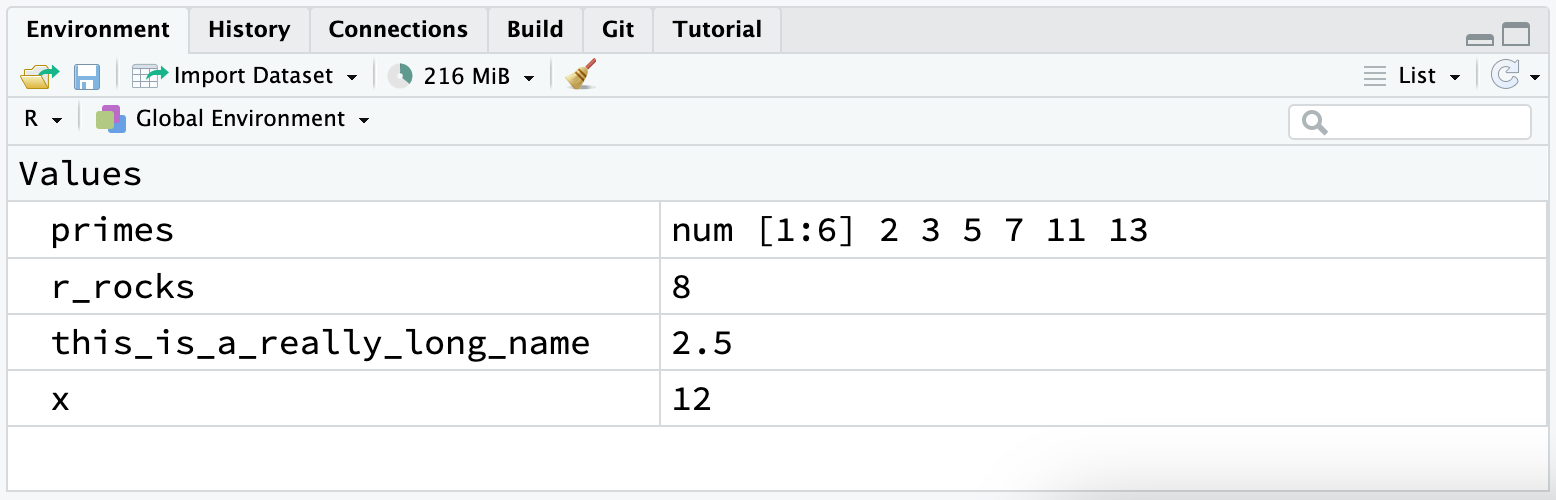
\includegraphics[width=2.59in,height=\textheight]{screenshots/rstudio-env.png}

\section{练习}\label{ux7ec3ux4e60-4}

\begin{enumerate}
\def\labelenumi{\arabic{enumi}.}
\item
  为什么这段代码不能正常运行?

\begin{Shaded}
\begin{Highlighting}[]
\NormalTok{my\_variable }\OtherTok{\textless{}{-}} \DecValTok{10}
\NormalTok{my\_varıable}
\CommentTok{\#\textgreater{} Error in eval(expr, envir, enclos): object \textquotesingle{}my\_varıable\textquotesingle{} not found}
\end{Highlighting}
\end{Shaded}

  仔细看!这
  可能看起来像是无意义的练习,但能训练你的大脑注意到即使是微小的差异,这在编程时也会让你有所受益。
\item
  微调以下每个 R 命令,以便它们可以正确运行:

\begin{Shaded}
\begin{Highlighting}[]
\FunctionTok{libary}\NormalTok{(todyverse)}

\FunctionTok{ggplot}\NormalTok{(}\AttributeTok{dTA =}\NormalTok{ mpg) }\SpecialCharTok{+} 
  \FunctionTok{geom\_point}\NormalTok{(}\AttributeTok{maping =} \FunctionTok{aes}\NormalTok{(}\AttributeTok{x =}\NormalTok{ displ }\AttributeTok{y =}\NormalTok{ hwy)) }\SpecialCharTok{+}
  \FunctionTok{geom\_smooth}\NormalTok{(}\AttributeTok{method =} \StringTok{"lm)}
\end{Highlighting}
\end{Shaded}
\item
  按下 Option + Shift + K / Alt + Shift + K,会发生什么?你
  如何通过菜单到达同样的地方?
\item
  重新看一下来自 小节~\ref{sec-ggsave} 的一个练习。运 行以下代码行。哪
  个图形被保存为 \texttt{mpg-plot.png}?为 什么?

\begin{Shaded}
\begin{Highlighting}[]
\NormalTok{my\_bar\_plot }\OtherTok{\textless{}{-}} \FunctionTok{ggplot}\NormalTok{(mpg, }\FunctionTok{aes}\NormalTok{(}\AttributeTok{x =}\NormalTok{ class)) }\SpecialCharTok{+}
  \FunctionTok{geom\_bar}\NormalTok{()}
\NormalTok{my\_scatter\_plot }\OtherTok{\textless{}{-}} \FunctionTok{ggplot}\NormalTok{(mpg, }\FunctionTok{aes}\NormalTok{(}\AttributeTok{x =}\NormalTok{ cty, }\AttributeTok{y =}\NormalTok{ hwy)) }\SpecialCharTok{+}
  \FunctionTok{geom\_point}\NormalTok{()}
\FunctionTok{ggsave}\NormalTok{(}\AttributeTok{filename =} \StringTok{"mpg{-}plot.png"}\NormalTok{, }\AttributeTok{plot =}\NormalTok{ my\_bar\_plot)}
\end{Highlighting}
\end{Shaded}
\end{enumerate}

\section{小结}\label{ux5c0fux7ed3-1}

现在你已经学习了更多关于R代码如何工作的知识以及一些提示。在
将来重新使用代码时这些提示能帮助你更好地理解它。在
下一章,我们将继续数据科学之旅,向你介绍dplyr,它是tidyverse的一个包,可以帮助你转换数据,例如选择重要的变量、筛选感兴趣的行还是计算汇总统计量。

\chapter{数据转换}\label{sec-data-transform}

\section{引言}\label{ux5f15ux8a00-1}

可视化是生成新见解的重要工具,但很少能刚好得到你所需的确切形式的数据来制作你想要的图。通
常,你需要创建一些新的变量或汇总统计量来用数据回答你的问题;或者你可能只是想重命名变量或重新排序观测值,以使数据更易于处理。在
本章中,你将学习如何做到这些(及更多)。本
章将介绍使用\textbf{dplyr}包和2013年从纽约市出发的航班数据集进行数据转换。

本章的目标是为你概述转换数据框的所有关键工具。我
们将从对数据框的行和列进行操作的函数开始,然后再次回到讨论管道(pipe),这是一个重要的工具,用于组合动词。接
下来,我们将介绍处理分组的能力。我
们将以一个研究案例结束本章,该案例研究展示了这些函数的实际应用;当我们开始深入研究特定类型的数据(例如数字、字符串、日期)时,我们将在后续的章节中更详细地讨论这些函数。

\subsection{必要条件}\label{ux5fc5ux8981ux6761ux4ef6-1}

本章将重点讨论dplyr包,它是tidyverse的另一个核心成员。我
们将使用来自nycflights13包的数据来说明dplyr包的关键理念,并使用ggplot2来帮助我们理解数据。

\begin{Shaded}
\begin{Highlighting}[]
\FunctionTok{library}\NormalTok{(nycflights13)}
\FunctionTok{library}\NormalTok{(tidyverse)}
\CommentTok{\#\textgreater{} {-}{-} Attaching core tidyverse packages {-}{-}{-}{-}{-}{-}{-}{-}{-}{-}{-}{-}{-}{-}{-}{-}{-}{-}{-}{-}{-} tidyverse 2.0.0 {-}{-}}
\CommentTok{\#\textgreater{} v dplyr     1.1.4     v readr     2.1.5}
\CommentTok{\#\textgreater{} v forcats   1.0.0     v stringr   1.5.1}
\CommentTok{\#\textgreater{} v ggplot2   3.5.0     v tibble    3.2.1}
\CommentTok{\#\textgreater{} v lubridate 1.9.3     v tidyr     1.3.1}
\CommentTok{\#\textgreater{} v purrr     1.0.2     }
\CommentTok{\#\textgreater{} {-}{-} Conflicts {-}{-}{-}{-}{-}{-}{-}{-}{-}{-}{-}{-}{-}{-}{-}{-}{-}{-}{-}{-}{-}{-}{-}{-}{-}{-}{-}{-}{-}{-}{-}{-}{-}{-}{-}{-}{-}{-}{-} tidyverse\_conflicts() {-}{-}}
\CommentTok{\#\textgreater{} x dplyr::filter() masks stats::filter()}
\CommentTok{\#\textgreater{} x dplyr::lag()    masks stats::lag()}
\CommentTok{\#\textgreater{} i Use the conflicted package (\textless{}http://conflicted.r{-}lib.org/\textgreater{}) to force all conflicts to become errors}
\end{Highlighting}
\end{Shaded}

请注意加载tidyverse时显示的冲突消息。它
告诉你dplyr覆盖了R基础包中的一些函数。如
果你在加载dplyr后想使用这些函数的基础版本,你需要使用它们的全名:stats::filter()
和 stats::lag()。到
目前为止,我们主要忽略了函数来自哪个包,因为大多数情况下这并不重要。但
是,知道包名可以帮助你找到帮助和相关的函数,所以当我们需要精确地知道一个函数来自哪个包时,我们将使用与R相同的语法:packagename::functionname()。

\subsection{nycflights13}\label{nycflights13}

为了探索基本的dplyr操作,我们将使用nycflights13::flights。此
数据集包含所有r format(nrow(nycflights13::flights), big.mark =
``,'')2013年从纽约出发的航班。这
些数据来自美国\href{https://www.transtats.bts.gov/DL_SelectFields.aspx?gnoyr_VQ=FGJ&QO_fu146_anzr=b0-gvzr}{Bureau
of Transportation Statistics},并记录在 ?f lights。

\begin{Shaded}
\begin{Highlighting}[]
\NormalTok{flights}
\CommentTok{\#\textgreater{} \# A tibble: 336,776 x 19}
\CommentTok{\#\textgreater{}    year month   day dep\_time sched\_dep\_time dep\_delay arr\_time sched\_arr\_time}
\CommentTok{\#\textgreater{}   \textless{}int\textgreater{} \textless{}int\textgreater{} \textless{}int\textgreater{}    \textless{}int\textgreater{}          \textless{}int\textgreater{}     \textless{}dbl\textgreater{}    \textless{}int\textgreater{}          \textless{}int\textgreater{}}
\CommentTok{\#\textgreater{} 1  2013     1     1      517            515         2      830            819}
\CommentTok{\#\textgreater{} 2  2013     1     1      533            529         4      850            830}
\CommentTok{\#\textgreater{} 3  2013     1     1      542            540         2      923            850}
\CommentTok{\#\textgreater{} 4  2013     1     1      544            545        {-}1     1004           1022}
\CommentTok{\#\textgreater{} 5  2013     1     1      554            600        {-}6      812            837}
\CommentTok{\#\textgreater{} 6  2013     1     1      554            558        {-}4      740            728}
\CommentTok{\#\textgreater{} \# i 336,770 more rows}
\CommentTok{\#\textgreater{} \# i 11 more variables: arr\_delay \textless{}dbl\textgreater{}, carrier \textless{}chr\textgreater{}, flight \textless{}int\textgreater{}, ...}
\end{Highlighting}
\end{Shaded}

flights是一个tibble(tibble是tidyverse使用的一种特殊类型的数据框),用于避免一些常见的意外情况。t
ibble和数据框之间最重要的区别在于它们的输出方式;tibble是为了大型数据集设计的,因此它们只显示前几行和能够在一个屏幕上显示的列。有
几种方法可以查看所有内容。如
果你正在使用RStudio,最方便的可能是View(flights),这会打开一个可以滚动和筛选的交互式视图。另
外你可以使用print(flights, width =
Inf)来显示所有列,或者使用glimpse()函数:

\begin{Shaded}
\begin{Highlighting}[]
\FunctionTok{glimpse}\NormalTok{(flights)}
\CommentTok{\#\textgreater{} Rows: 336,776}
\CommentTok{\#\textgreater{} Columns: 19}
\CommentTok{\#\textgreater{} $ year           \textless{}int\textgreater{} 2013, 2013, 2013, 2013, 2013, 2013, 2013, 2013, 2013\textasciitilde{}}
\CommentTok{\#\textgreater{} $ month          \textless{}int\textgreater{} 1, 1, 1, 1, 1, 1, 1, 1, 1, 1, 1, 1, 1, 1, 1, 1, 1, 1\textasciitilde{}}
\CommentTok{\#\textgreater{} $ day            \textless{}int\textgreater{} 1, 1, 1, 1, 1, 1, 1, 1, 1, 1, 1, 1, 1, 1, 1, 1, 1, 1\textasciitilde{}}
\CommentTok{\#\textgreater{} $ dep\_time       \textless{}int\textgreater{} 517, 533, 542, 544, 554, 554, 555, 557, 557, 558, 55\textasciitilde{}}
\CommentTok{\#\textgreater{} $ sched\_dep\_time \textless{}int\textgreater{} 515, 529, 540, 545, 600, 558, 600, 600, 600, 600, 60\textasciitilde{}}
\CommentTok{\#\textgreater{} $ dep\_delay      \textless{}dbl\textgreater{} 2, 4, 2, {-}1, {-}6, {-}4, {-}5, {-}3, {-}3, {-}2, {-}2, {-}2, {-}2, {-}2,\textasciitilde{}}
\CommentTok{\#\textgreater{} $ arr\_time       \textless{}int\textgreater{} 830, 850, 923, 1004, 812, 740, 913, 709, 838, 753, 8\textasciitilde{}}
\CommentTok{\#\textgreater{} $ sched\_arr\_time \textless{}int\textgreater{} 819, 830, 850, 1022, 837, 728, 854, 723, 846, 745, 8\textasciitilde{}}
\CommentTok{\#\textgreater{} $ arr\_delay      \textless{}dbl\textgreater{} 11, 20, 33, {-}18, {-}25, 12, 19, {-}14, {-}8, 8, {-}2, {-}3, 7,\textasciitilde{}}
\CommentTok{\#\textgreater{} $ carrier        \textless{}chr\textgreater{} "UA", "UA", "AA", "B6", "DL", "UA", "B6", "EV", "B6"\textasciitilde{}}
\CommentTok{\#\textgreater{} $ flight         \textless{}int\textgreater{} 1545, 1714, 1141, 725, 461, 1696, 507, 5708, 79, 301\textasciitilde{}}
\CommentTok{\#\textgreater{} $ tailnum        \textless{}chr\textgreater{} "N14228", "N24211", "N619AA", "N804JB", "N668DN", "N\textasciitilde{}}
\CommentTok{\#\textgreater{} $ origin         \textless{}chr\textgreater{} "EWR", "LGA", "JFK", "JFK", "LGA", "EWR", "EWR", "LG\textasciitilde{}}
\CommentTok{\#\textgreater{} $ dest           \textless{}chr\textgreater{} "IAH", "IAH", "MIA", "BQN", "ATL", "ORD", "FLL", "IA\textasciitilde{}}
\CommentTok{\#\textgreater{} $ air\_time       \textless{}dbl\textgreater{} 227, 227, 160, 183, 116, 150, 158, 53, 140, 138, 149\textasciitilde{}}
\CommentTok{\#\textgreater{} $ distance       \textless{}dbl\textgreater{} 1400, 1416, 1089, 1576, 762, 719, 1065, 229, 944, 73\textasciitilde{}}
\CommentTok{\#\textgreater{} $ hour           \textless{}dbl\textgreater{} 5, 5, 5, 5, 6, 5, 6, 6, 6, 6, 6, 6, 6, 6, 6, 5, 6, 6\textasciitilde{}}
\CommentTok{\#\textgreater{} $ minute         \textless{}dbl\textgreater{} 15, 29, 40, 45, 0, 58, 0, 0, 0, 0, 0, 0, 0, 0, 0, 59\textasciitilde{}}
\CommentTok{\#\textgreater{} $ time\_hour      \textless{}dttm\textgreater{} 2013{-}01{-}01 05:00:00, 2013{-}01{-}01 05:00:00, 2013{-}01{-}0\textasciitilde{}}
\end{Highlighting}
\end{Shaded}

在这两种视图中,变量名后面跟着缩写,这些缩写表示每个变量的类型:\textless int\textgreater 是整数的缩写,\textless dbl\textgreater 是双精度浮点数(也称为实数)的缩写,\textless chr\textgreater 是字符(也称为字符串)的缩写,\textless dttm\textgreater 是日期时间的缩写。这
些缩写很重要,因为你可以在一列上执行的操作在很大程度上取决于它的``类型''。

\subsection{dplyr 基础}\label{dplyr-ux57faux7840}

下面将学习dplyr的主要操作(即函数),这些函数能帮你解决绝大多数的数据处理问题。但
在讨论它们各自的差异之前,值得一提的是它们的共同点:

\begin{enumerate}
\def\labelenumi{\arabic{enumi}.}
\tightlist
\item
  第一个参数始终是一个数据框;
\item
  后续参数通常使用变量名(不带引号)来描述要操作的列;
\item
  输出始终是一个新的数据框。
\end{enumerate}

因为每个函数都擅长做一件事,所以解决复杂问题通常需要组合多个函数,我们将使用管道操作符\textbar\textgreater 来实现这一点。我
们将在@sec-the-pipe 更详细地讨论管道操作符。简
言之,管道操作符将其左侧的内容传递给其右侧的函数,因此x
\textbar\textgreater{} f(y)等同于f(x, y),而x \textbar\textgreater{}
f(y) \textbar\textgreater{} g(z)等同于g(f(x, y),
z),\textbar\textgreater 最简单的发音是``then''。这
使得即使你还没有学习细节,也有可能理解下面的代码:

\begin{Shaded}
\begin{Highlighting}[]
\NormalTok{flights }\SpecialCharTok{|\textgreater{}}
  \FunctionTok{filter}\NormalTok{(dest }\SpecialCharTok{==} \StringTok{"IAH"}\NormalTok{) }\SpecialCharTok{|\textgreater{}} 
  \FunctionTok{group\_by}\NormalTok{(year, month, day) }\SpecialCharTok{|\textgreater{}} 
  \FunctionTok{summarize}\NormalTok{(}
    \AttributeTok{arr\_delay =} \FunctionTok{mean}\NormalTok{(arr\_delay, }\AttributeTok{na.rm =} \ConstantTok{TRUE}\NormalTok{)}
\NormalTok{  )}
\end{Highlighting}
\end{Shaded}

dplyr的函数根据作用对象不同分为四组:\textbf{行}(rows)、\textbf{列}(columns)、\textbf{组}(groups)或\textbf{表}(tables)。下
面将学习有关行、列和组的最重要函数,然后回到@sec-joins
中探讨作用于表的合并操作。让 我们开始吧!

\section{行}\label{ux884c}

对数据集的行进行操作的最重要的函数是filter(),它影响行的去留而不改变它们的顺序;而函数arrange()改变行的顺序而不影响行的去留。这
两个函数都只影响行,列保持不变。我
们还将讨论distinct(),它找出具有唯一值的行,但与arrange()和filter()不同,它还可以选择性地修改列。

\subsection{filter()}\label{filter}

Filter()允许你根据列的值保留行\footnote{稍后,您将学习\texttt{slice\_*()系列}函数,它允许你根据行的位置选择行。}。
第一个参数是数据框,第二个及随后的参数是保留该行必须为真的条件。
例如,我们可以找出所有迟到超过120分钟(2小时)的航班:

\begin{Shaded}
\begin{Highlighting}[]
\NormalTok{flights }\SpecialCharTok{|\textgreater{}} 
  \FunctionTok{filter}\NormalTok{(dep\_delay }\SpecialCharTok{\textgreater{}} \DecValTok{120}\NormalTok{)}
\CommentTok{\#\textgreater{} \# A tibble: 9,723 x 19}
\CommentTok{\#\textgreater{}    year month   day dep\_time sched\_dep\_time dep\_delay arr\_time sched\_arr\_time}
\CommentTok{\#\textgreater{}   \textless{}int\textgreater{} \textless{}int\textgreater{} \textless{}int\textgreater{}    \textless{}int\textgreater{}          \textless{}int\textgreater{}     \textless{}dbl\textgreater{}    \textless{}int\textgreater{}          \textless{}int\textgreater{}}
\CommentTok{\#\textgreater{} 1  2013     1     1      848           1835       853     1001           1950}
\CommentTok{\#\textgreater{} 2  2013     1     1      957            733       144     1056            853}
\CommentTok{\#\textgreater{} 3  2013     1     1     1114            900       134     1447           1222}
\CommentTok{\#\textgreater{} 4  2013     1     1     1540           1338       122     2020           1825}
\CommentTok{\#\textgreater{} 5  2013     1     1     1815           1325       290     2120           1542}
\CommentTok{\#\textgreater{} 6  2013     1     1     1842           1422       260     1958           1535}
\CommentTok{\#\textgreater{} \# i 9,717 more rows}
\CommentTok{\#\textgreater{} \# i 11 more variables: arr\_delay \textless{}dbl\textgreater{}, carrier \textless{}chr\textgreater{}, flight \textless{}int\textgreater{}, ...}
\end{Highlighting}
\end{Shaded}

除了使用 \textgreater(大于)之外,还可以使用
\textgreater=(大于或等于)、\textless(小于)、\textless=(小于或等于)、==(等于)和
!= (不等于)。你 还可以使用 \& 或 ,
来组合条件,表示``和''(检查两个条件是否都满足),或者使用 \textbar{}
来表示``或''(检查任一条件是否满足):

\begin{Shaded}
\begin{Highlighting}[]
\CommentTok{\# Flights that departed on January 1}
\NormalTok{flights }\SpecialCharTok{|\textgreater{}} 
  \FunctionTok{filter}\NormalTok{(month }\SpecialCharTok{==} \DecValTok{1} \SpecialCharTok{\&}\NormalTok{ day }\SpecialCharTok{==} \DecValTok{1}\NormalTok{)}
\CommentTok{\#\textgreater{} \# A tibble: 842 x 19}
\CommentTok{\#\textgreater{}    year month   day dep\_time sched\_dep\_time dep\_delay arr\_time sched\_arr\_time}
\CommentTok{\#\textgreater{}   \textless{}int\textgreater{} \textless{}int\textgreater{} \textless{}int\textgreater{}    \textless{}int\textgreater{}          \textless{}int\textgreater{}     \textless{}dbl\textgreater{}    \textless{}int\textgreater{}          \textless{}int\textgreater{}}
\CommentTok{\#\textgreater{} 1  2013     1     1      517            515         2      830            819}
\CommentTok{\#\textgreater{} 2  2013     1     1      533            529         4      850            830}
\CommentTok{\#\textgreater{} 3  2013     1     1      542            540         2      923            850}
\CommentTok{\#\textgreater{} 4  2013     1     1      544            545        {-}1     1004           1022}
\CommentTok{\#\textgreater{} 5  2013     1     1      554            600        {-}6      812            837}
\CommentTok{\#\textgreater{} 6  2013     1     1      554            558        {-}4      740            728}
\CommentTok{\#\textgreater{} \# i 836 more rows}
\CommentTok{\#\textgreater{} \# i 11 more variables: arr\_delay \textless{}dbl\textgreater{}, carrier \textless{}chr\textgreater{}, flight \textless{}int\textgreater{}, ...}

\CommentTok{\# Flights that departed in January or February}
\NormalTok{flights }\SpecialCharTok{|\textgreater{}} 
  \FunctionTok{filter}\NormalTok{(month }\SpecialCharTok{==} \DecValTok{1} \SpecialCharTok{|}\NormalTok{ month }\SpecialCharTok{==} \DecValTok{2}\NormalTok{)}
\CommentTok{\#\textgreater{} \# A tibble: 51,955 x 19}
\CommentTok{\#\textgreater{}    year month   day dep\_time sched\_dep\_time dep\_delay arr\_time sched\_arr\_time}
\CommentTok{\#\textgreater{}   \textless{}int\textgreater{} \textless{}int\textgreater{} \textless{}int\textgreater{}    \textless{}int\textgreater{}          \textless{}int\textgreater{}     \textless{}dbl\textgreater{}    \textless{}int\textgreater{}          \textless{}int\textgreater{}}
\CommentTok{\#\textgreater{} 1  2013     1     1      517            515         2      830            819}
\CommentTok{\#\textgreater{} 2  2013     1     1      533            529         4      850            830}
\CommentTok{\#\textgreater{} 3  2013     1     1      542            540         2      923            850}
\CommentTok{\#\textgreater{} 4  2013     1     1      544            545        {-}1     1004           1022}
\CommentTok{\#\textgreater{} 5  2013     1     1      554            600        {-}6      812            837}
\CommentTok{\#\textgreater{} 6  2013     1     1      554            558        {-}4      740            728}
\CommentTok{\#\textgreater{} \# i 51,949 more rows}
\CommentTok{\#\textgreater{} \# i 11 more variables: arr\_delay \textless{}dbl\textgreater{}, carrier \textless{}chr\textgreater{}, flight \textless{}int\textgreater{}, ...}
\end{Highlighting}
\end{Shaded}

当您结合使用 \textbar{} 和 == 时有一个很有用的快捷方式:\%in\%。它
会保留变量等于右侧值之一的行:

\begin{Shaded}
\begin{Highlighting}[]
\CommentTok{\# A shorter way to select flights that departed in January or February}
\NormalTok{flights }\SpecialCharTok{|\textgreater{}} 
  \FunctionTok{filter}\NormalTok{(month }\SpecialCharTok{\%in\%} \FunctionTok{c}\NormalTok{(}\DecValTok{1}\NormalTok{, }\DecValTok{2}\NormalTok{))}
\CommentTok{\#\textgreater{} \# A tibble: 51,955 x 19}
\CommentTok{\#\textgreater{}    year month   day dep\_time sched\_dep\_time dep\_delay arr\_time sched\_arr\_time}
\CommentTok{\#\textgreater{}   \textless{}int\textgreater{} \textless{}int\textgreater{} \textless{}int\textgreater{}    \textless{}int\textgreater{}          \textless{}int\textgreater{}     \textless{}dbl\textgreater{}    \textless{}int\textgreater{}          \textless{}int\textgreater{}}
\CommentTok{\#\textgreater{} 1  2013     1     1      517            515         2      830            819}
\CommentTok{\#\textgreater{} 2  2013     1     1      533            529         4      850            830}
\CommentTok{\#\textgreater{} 3  2013     1     1      542            540         2      923            850}
\CommentTok{\#\textgreater{} 4  2013     1     1      544            545        {-}1     1004           1022}
\CommentTok{\#\textgreater{} 5  2013     1     1      554            600        {-}6      812            837}
\CommentTok{\#\textgreater{} 6  2013     1     1      554            558        {-}4      740            728}
\CommentTok{\#\textgreater{} \# i 51,949 more rows}
\CommentTok{\#\textgreater{} \# i 11 more variables: arr\_delay \textless{}dbl\textgreater{}, carrier \textless{}chr\textgreater{}, flight \textless{}int\textgreater{}, ...}
\end{Highlighting}
\end{Shaded}

我们将在@sec-logicals 中详细讨论这些比较和逻辑运算符。

当你运行filter()时,dplyr会执行筛选操作,创建一个新的数据框,然后输出它。它
不会修改现有的flights数据集,因为dplyr函数永远不会修改它们的输入。要
保存结果,你需要使用赋值运算符\textless-:

\begin{Shaded}
\begin{Highlighting}[]
\NormalTok{jan1 }\OtherTok{\textless{}{-}}\NormalTok{ flights }\SpecialCharTok{|\textgreater{}} 
  \FunctionTok{filter}\NormalTok{(month }\SpecialCharTok{==} \DecValTok{1} \SpecialCharTok{\&}\NormalTok{ day }\SpecialCharTok{==} \DecValTok{1}\NormalTok{)}
\end{Highlighting}
\end{Shaded}

\subsection{常见错误}\label{ux5e38ux89c1ux9519ux8bef}

从你刚开始学习R时,最容易犯的错误是在检验是否相等时使用=而不是==。f
ilter()会告诉你发生了什么:

\begin{Shaded}
\begin{Highlighting}[]
\NormalTok{flights }\SpecialCharTok{|\textgreater{}} 
  \FunctionTok{filter}\NormalTok{(}\AttributeTok{month =} \DecValTok{1}\NormalTok{)}
\CommentTok{\#\textgreater{} Error in \textasciigrave{}filter()\textasciigrave{}:}
\CommentTok{\#\textgreater{} ! We detected a named input.}
\CommentTok{\#\textgreater{} i This usually means that you\textquotesingle{}ve used \textasciigrave{}=\textasciigrave{} instead of \textasciigrave{}==\textasciigrave{}.}
\CommentTok{\#\textgreater{} i Did you mean \textasciigrave{}month == 1\textasciigrave{}?}
\end{Highlighting}
\end{Shaded}

另一个错误是像在英语中那样写``或''语句:

\begin{Shaded}
\begin{Highlighting}[]
\NormalTok{flights }\SpecialCharTok{|\textgreater{}} 
  \FunctionTok{filter}\NormalTok{(month }\SpecialCharTok{==} \DecValTok{1} \SpecialCharTok{|} \DecValTok{2}\NormalTok{)}
\end{Highlighting}
\end{Shaded}

这段代码``有效'',它不会抛出错误,但它没有按照你的期望去做,因为
\textbar{} 首先检查条件month ==
1,然后检查条件2,而检查2并不是一个合理的条件。我 们将在
小节~\ref{sec-boolean-operations} 更多地了解这里发生了什么,以及为什么。

\subsection{arrange()}\label{arrange}

arrange()根据列的值改变行的顺序。它
根据一个数据框和一组列名(或更复杂的表达式)来排序。如
果你提供了多个列名,那么每个额外的列都将用于解决前面列中值的并列问题。例
如,下面的代码按出发时间排序,出发时间分布在四个列中。我
们首先得到最早的年份,然后在同一年份中,我们得到最早的月份,依此类推。

\begin{Shaded}
\begin{Highlighting}[]
\NormalTok{flights }\SpecialCharTok{|\textgreater{}} 
  \FunctionTok{arrange}\NormalTok{(year, month, day, dep\_time)}
\CommentTok{\#\textgreater{} \# A tibble: 336,776 x 19}
\CommentTok{\#\textgreater{}    year month   day dep\_time sched\_dep\_time dep\_delay arr\_time sched\_arr\_time}
\CommentTok{\#\textgreater{}   \textless{}int\textgreater{} \textless{}int\textgreater{} \textless{}int\textgreater{}    \textless{}int\textgreater{}          \textless{}int\textgreater{}     \textless{}dbl\textgreater{}    \textless{}int\textgreater{}          \textless{}int\textgreater{}}
\CommentTok{\#\textgreater{} 1  2013     1     1      517            515         2      830            819}
\CommentTok{\#\textgreater{} 2  2013     1     1      533            529         4      850            830}
\CommentTok{\#\textgreater{} 3  2013     1     1      542            540         2      923            850}
\CommentTok{\#\textgreater{} 4  2013     1     1      544            545        {-}1     1004           1022}
\CommentTok{\#\textgreater{} 5  2013     1     1      554            600        {-}6      812            837}
\CommentTok{\#\textgreater{} 6  2013     1     1      554            558        {-}4      740            728}
\CommentTok{\#\textgreater{} \# i 336,770 more rows}
\CommentTok{\#\textgreater{} \# i 11 more variables: arr\_delay \textless{}dbl\textgreater{}, carrier \textless{}chr\textgreater{}, flight \textless{}int\textgreater{}, ...}
\end{Highlighting}
\end{Shaded}

你可以在arrange()内部对某一列使用desc()来根据该列的值以降序(从大到小)重新排序数据框。例
如,这段代码将航班按延误时间从长到短排序:

\begin{Shaded}
\begin{Highlighting}[]
\NormalTok{flights }\SpecialCharTok{|\textgreater{}} 
  \FunctionTok{arrange}\NormalTok{(}\FunctionTok{desc}\NormalTok{(dep\_delay))}
\CommentTok{\#\textgreater{} \# A tibble: 336,776 x 19}
\CommentTok{\#\textgreater{}    year month   day dep\_time sched\_dep\_time dep\_delay arr\_time sched\_arr\_time}
\CommentTok{\#\textgreater{}   \textless{}int\textgreater{} \textless{}int\textgreater{} \textless{}int\textgreater{}    \textless{}int\textgreater{}          \textless{}int\textgreater{}     \textless{}dbl\textgreater{}    \textless{}int\textgreater{}          \textless{}int\textgreater{}}
\CommentTok{\#\textgreater{} 1  2013     1     9      641            900      1301     1242           1530}
\CommentTok{\#\textgreater{} 2  2013     6    15     1432           1935      1137     1607           2120}
\CommentTok{\#\textgreater{} 3  2013     1    10     1121           1635      1126     1239           1810}
\CommentTok{\#\textgreater{} 4  2013     9    20     1139           1845      1014     1457           2210}
\CommentTok{\#\textgreater{} 5  2013     7    22      845           1600      1005     1044           1815}
\CommentTok{\#\textgreater{} 6  2013     4    10     1100           1900       960     1342           2211}
\CommentTok{\#\textgreater{} \# i 336,770 more rows}
\CommentTok{\#\textgreater{} \# i 11 more variables: arr\_delay \textless{}dbl\textgreater{}, carrier \textless{}chr\textgreater{}, flight \textless{}int\textgreater{}, ...}
\end{Highlighting}
\end{Shaded}

注意,行数没有改变,我们只是对数据进行了排列,没有对其进行过筛选。

\subsection{distinct()}\label{distinct}

distinct()在数据集中找出所有唯一的行,所以从技术上讲,它主要对行进行操作。然
而,在大多数情况下,你会想要某些变量的不同组合,因此你也可以选择性地提供列名:

\begin{Shaded}
\begin{Highlighting}[]
\CommentTok{\# Remove duplicate rows, if any}
\NormalTok{flights }\SpecialCharTok{|\textgreater{}} 
  \FunctionTok{distinct}\NormalTok{()}
\CommentTok{\#\textgreater{} \# A tibble: 336,776 x 19}
\CommentTok{\#\textgreater{}    year month   day dep\_time sched\_dep\_time dep\_delay arr\_time sched\_arr\_time}
\CommentTok{\#\textgreater{}   \textless{}int\textgreater{} \textless{}int\textgreater{} \textless{}int\textgreater{}    \textless{}int\textgreater{}          \textless{}int\textgreater{}     \textless{}dbl\textgreater{}    \textless{}int\textgreater{}          \textless{}int\textgreater{}}
\CommentTok{\#\textgreater{} 1  2013     1     1      517            515         2      830            819}
\CommentTok{\#\textgreater{} 2  2013     1     1      533            529         4      850            830}
\CommentTok{\#\textgreater{} 3  2013     1     1      542            540         2      923            850}
\CommentTok{\#\textgreater{} 4  2013     1     1      544            545        {-}1     1004           1022}
\CommentTok{\#\textgreater{} 5  2013     1     1      554            600        {-}6      812            837}
\CommentTok{\#\textgreater{} 6  2013     1     1      554            558        {-}4      740            728}
\CommentTok{\#\textgreater{} \# i 336,770 more rows}
\CommentTok{\#\textgreater{} \# i 11 more variables: arr\_delay \textless{}dbl\textgreater{}, carrier \textless{}chr\textgreater{}, flight \textless{}int\textgreater{}, ...}

\CommentTok{\# Find all unique origin and destination pairs}
\NormalTok{flights }\SpecialCharTok{|\textgreater{}} 
  \FunctionTok{distinct}\NormalTok{(origin, dest)}
\CommentTok{\#\textgreater{} \# A tibble: 224 x 2}
\CommentTok{\#\textgreater{}   origin dest }
\CommentTok{\#\textgreater{}   \textless{}chr\textgreater{}  \textless{}chr\textgreater{}}
\CommentTok{\#\textgreater{} 1 EWR    IAH  }
\CommentTok{\#\textgreater{} 2 LGA    IAH  }
\CommentTok{\#\textgreater{} 3 JFK    MIA  }
\CommentTok{\#\textgreater{} 4 JFK    BQN  }
\CommentTok{\#\textgreater{} 5 LGA    ATL  }
\CommentTok{\#\textgreater{} 6 EWR    ORD  }
\CommentTok{\#\textgreater{} \# i 218 more rows}
\end{Highlighting}
\end{Shaded}

或者,如果希望在筛选唯一行时保留其他列,您可以使用.keep\_all =
TRUE选项。

\begin{Shaded}
\begin{Highlighting}[]
\NormalTok{flights }\SpecialCharTok{|\textgreater{}} 
  \FunctionTok{distinct}\NormalTok{(origin, dest, }\AttributeTok{.keep\_all =} \ConstantTok{TRUE}\NormalTok{)}
\CommentTok{\#\textgreater{} \# A tibble: 224 x 19}
\CommentTok{\#\textgreater{}    year month   day dep\_time sched\_dep\_time dep\_delay arr\_time sched\_arr\_time}
\CommentTok{\#\textgreater{}   \textless{}int\textgreater{} \textless{}int\textgreater{} \textless{}int\textgreater{}    \textless{}int\textgreater{}          \textless{}int\textgreater{}     \textless{}dbl\textgreater{}    \textless{}int\textgreater{}          \textless{}int\textgreater{}}
\CommentTok{\#\textgreater{} 1  2013     1     1      517            515         2      830            819}
\CommentTok{\#\textgreater{} 2  2013     1     1      533            529         4      850            830}
\CommentTok{\#\textgreater{} 3  2013     1     1      542            540         2      923            850}
\CommentTok{\#\textgreater{} 4  2013     1     1      544            545        {-}1     1004           1022}
\CommentTok{\#\textgreater{} 5  2013     1     1      554            600        {-}6      812            837}
\CommentTok{\#\textgreater{} 6  2013     1     1      554            558        {-}4      740            728}
\CommentTok{\#\textgreater{} \# i 218 more rows}
\CommentTok{\#\textgreater{} \# i 11 more variables: arr\_delay \textless{}dbl\textgreater{}, carrier \textless{}chr\textgreater{}, flight \textless{}int\textgreater{}, ...}
\end{Highlighting}
\end{Shaded}

所有这些不同的航班都在1月1日并不是巧合:distinct()会在数据集中找到第一个出现的唯一行,并丢弃其余的行。

如果你想要找到出现的次数,那么最好将distinct()替换为count(),并使用sort
= TRUE参数,你可以按照出现次数的降序排列它们。你 将在
小节~\ref{sec-counts} 学到更多关于count的内容。

\begin{Shaded}
\begin{Highlighting}[]
\NormalTok{flights }\SpecialCharTok{|\textgreater{}}
  \FunctionTok{count}\NormalTok{(origin, dest, }\AttributeTok{sort =} \ConstantTok{TRUE}\NormalTok{)}
\CommentTok{\#\textgreater{} \# A tibble: 224 x 3}
\CommentTok{\#\textgreater{}   origin dest      n}
\CommentTok{\#\textgreater{}   \textless{}chr\textgreater{}  \textless{}chr\textgreater{} \textless{}int\textgreater{}}
\CommentTok{\#\textgreater{} 1 JFK    LAX   11262}
\CommentTok{\#\textgreater{} 2 LGA    ATL   10263}
\CommentTok{\#\textgreater{} 3 LGA    ORD    8857}
\CommentTok{\#\textgreater{} 4 JFK    SFO    8204}
\CommentTok{\#\textgreater{} 5 LGA    CLT    6168}
\CommentTok{\#\textgreater{} 6 EWR    ORD    6100}
\CommentTok{\#\textgreater{} \# i 218 more rows}
\end{Highlighting}
\end{Shaded}

\subsection{练习}\label{ux7ec3ux4e60-5}

\begin{enumerate}
\def\labelenumi{\arabic{enumi}.}
\item
  针对每个条件,在单个管道中查找所有符合以下条件的航班:

  \begin{itemize}
  \tightlist
  \item
    到达延误两小时或更长时间
  \item
    飞往休斯敦(IAH或HOU)
  \item
    由联合航空(United)、美国航空(American),或达美航空(Delta)运营
  \item
    在夏季(七月、八月和九月)起飞
  \item
    到达延误超过两小时,但起飞不延误
  \item
    延误至少一小时,但在飞行中弥补了超过30分钟的时间
  \end{itemize}
\item
  对flights
  进行排序以找到出发延误时间最长的航班;找到早上最早起飞的航班;
\item
  对flights进行排序以找到最快的航班。( 提示:
  尝试在函数中包含数学计算。)
\item
  2013年的每一天都有航班吗?
\item
  哪些航班飞行了最远的距离?哪 些飞行了最短的距离?
\item
  如果你同时使用filter()和arrange(),你使用的顺序重要吗?为 什么?思
  考一下结果以及这些函数需要执行多少工作。
\end{enumerate}

\section{列}\label{ux5217}

有四个重要的函数,它们影响列而不改变行:mutate()用于根据现有列创建新列,select()用于更改列存留,rename()用于更改列的名称,而relocate()用于更改列的位置。

\subsection{mutate()}\label{sec-mutate}

mutate()的作用是添加根据现有列计算得到的新列。在
数据转换章节中,你将学习一系列函数,这些函数可用于处理不同类型的变量。目
前,我们将继续使用基础代数,这允许我们计算gain(即延误航班在空中弥补了多少时间)以及每小时的速度:

\begin{Shaded}
\begin{Highlighting}[]
\NormalTok{flights }\SpecialCharTok{|\textgreater{}} 
  \FunctionTok{mutate}\NormalTok{(}
    \AttributeTok{gain =}\NormalTok{ dep\_delay }\SpecialCharTok{{-}}\NormalTok{ arr\_delay,}
    \AttributeTok{speed =}\NormalTok{ distance }\SpecialCharTok{/}\NormalTok{ air\_time }\SpecialCharTok{*} \DecValTok{60}
\NormalTok{  )}
\CommentTok{\#\textgreater{} \# A tibble: 336,776 x 21}
\CommentTok{\#\textgreater{}    year month   day dep\_time sched\_dep\_time dep\_delay arr\_time sched\_arr\_time}
\CommentTok{\#\textgreater{}   \textless{}int\textgreater{} \textless{}int\textgreater{} \textless{}int\textgreater{}    \textless{}int\textgreater{}          \textless{}int\textgreater{}     \textless{}dbl\textgreater{}    \textless{}int\textgreater{}          \textless{}int\textgreater{}}
\CommentTok{\#\textgreater{} 1  2013     1     1      517            515         2      830            819}
\CommentTok{\#\textgreater{} 2  2013     1     1      533            529         4      850            830}
\CommentTok{\#\textgreater{} 3  2013     1     1      542            540         2      923            850}
\CommentTok{\#\textgreater{} 4  2013     1     1      544            545        {-}1     1004           1022}
\CommentTok{\#\textgreater{} 5  2013     1     1      554            600        {-}6      812            837}
\CommentTok{\#\textgreater{} 6  2013     1     1      554            558        {-}4      740            728}
\CommentTok{\#\textgreater{} \# i 336,770 more rows}
\CommentTok{\#\textgreater{} \# i 13 more variables: arr\_delay \textless{}dbl\textgreater{}, carrier \textless{}chr\textgreater{}, flight \textless{}int\textgreater{}, ...}
\end{Highlighting}
\end{Shaded}

默认情况下,mutate()会在数据集的右侧添加新列,但这使得我们很难看到数据集里发生了什么。可
以使用.before参数来将变量添加到左侧:

By default, mutate() adds new columns on the right hand side of your
dataset, which makes it difficult to see what's happening here. We can
use the .before argument to instead add the variables to the left hand
side\footnote{Remember that in RStudio, the easiest way to see a dataset
  with many columns is \texttt{View()}.}:

\begin{Shaded}
\begin{Highlighting}[]
\NormalTok{flights }\SpecialCharTok{|\textgreater{}} 
  \FunctionTok{mutate}\NormalTok{(}
    \AttributeTok{gain =}\NormalTok{ dep\_delay }\SpecialCharTok{{-}}\NormalTok{ arr\_delay,}
    \AttributeTok{speed =}\NormalTok{ distance }\SpecialCharTok{/}\NormalTok{ air\_time }\SpecialCharTok{*} \DecValTok{60}\NormalTok{,}
    \AttributeTok{.before =} \DecValTok{1}
\NormalTok{  )}
\CommentTok{\#\textgreater{} \# A tibble: 336,776 x 21}
\CommentTok{\#\textgreater{}    gain speed  year month   day dep\_time sched\_dep\_time dep\_delay arr\_time}
\CommentTok{\#\textgreater{}   \textless{}dbl\textgreater{} \textless{}dbl\textgreater{} \textless{}int\textgreater{} \textless{}int\textgreater{} \textless{}int\textgreater{}    \textless{}int\textgreater{}          \textless{}int\textgreater{}     \textless{}dbl\textgreater{}    \textless{}int\textgreater{}}
\CommentTok{\#\textgreater{} 1    {-}9  370.  2013     1     1      517            515         2      830}
\CommentTok{\#\textgreater{} 2   {-}16  374.  2013     1     1      533            529         4      850}
\CommentTok{\#\textgreater{} 3   {-}31  408.  2013     1     1      542            540         2      923}
\CommentTok{\#\textgreater{} 4    17  517.  2013     1     1      544            545        {-}1     1004}
\CommentTok{\#\textgreater{} 5    19  394.  2013     1     1      554            600        {-}6      812}
\CommentTok{\#\textgreater{} 6   {-}16  288.  2013     1     1      554            558        {-}4      740}
\CommentTok{\#\textgreater{} \# i 336,770 more rows}
\CommentTok{\#\textgreater{} \# i 12 more variables: sched\_arr\_time \textless{}int\textgreater{}, arr\_delay \textless{}dbl\textgreater{}, ...}
\end{Highlighting}
\end{Shaded}

.是一个标志,表示.before~是函数的参数,而不是我们正在创建的第三个新变量的名称。你
也可以使用.after在某个变量之后添加新变量,在.before和.after中,你都可以使用变量名而不是位置。例
如,我们可以在day之后添加新变量:

\begin{Shaded}
\begin{Highlighting}[]
\NormalTok{flights }\SpecialCharTok{|\textgreater{}} 
  \FunctionTok{mutate}\NormalTok{(}
    \AttributeTok{gain =}\NormalTok{ dep\_delay }\SpecialCharTok{{-}}\NormalTok{ arr\_delay,}
    \AttributeTok{speed =}\NormalTok{ distance }\SpecialCharTok{/}\NormalTok{ air\_time }\SpecialCharTok{*} \DecValTok{60}\NormalTok{,}
    \AttributeTok{.after =}\NormalTok{ day}
\NormalTok{  )}
\end{Highlighting}
\end{Shaded}

另外,你可以使用.keep参数来控制保留哪些变量。一
个特别有用的参数是''used'',它指定我们只保留在mutate()步骤中涉及或创建的列。例
如,以下输出将仅包含dep\_delay、arr\_delay、air\_time、gain、hours和gain\_per\_hour这些变量。

\begin{Shaded}
\begin{Highlighting}[]
\NormalTok{flights }\SpecialCharTok{|\textgreater{}} 
  \FunctionTok{mutate}\NormalTok{(}
    \AttributeTok{gain =}\NormalTok{ dep\_delay }\SpecialCharTok{{-}}\NormalTok{ arr\_delay,}
    \AttributeTok{hours =}\NormalTok{ air\_time }\SpecialCharTok{/} \DecValTok{60}\NormalTok{,}
    \AttributeTok{gain\_per\_hour =}\NormalTok{ gain }\SpecialCharTok{/}\NormalTok{ hours,}
    \AttributeTok{.keep =} \StringTok{"used"}
\NormalTok{  )}
\end{Highlighting}
\end{Shaded}

请注意,由于我们没有将上述计算的结果重新分配给flights数据框,新的变量gain、hours和gain\_per\_hour只会被输出出来,但不会被存储在一个数据框中。如
果我们希望这些变量在未来的数据框中可用,我们应该仔细考虑是否要将结果重新分配给flights,从而用更多的变量覆盖原始数据框,还是分配给一个新的对象。通
常,正确的答案是创建一个新的对象,并为其命名以清晰地指示其内容,例如delay\_gain,但你也可能有充分的理由覆盖flights。

\subsection{select()}\label{sec-select}

获得包含数百甚至数千个变量的数据集并不罕见。在
这种情况下,第一个挑战通常是仅关注你感兴趣的变量。s
elect()允许你基于变量的名称,通过操作快速缩小到一个有用的子集:

\begin{itemize}
\item
  按名称选择列:

\begin{Shaded}
\begin{Highlighting}[]
\NormalTok{flights }\SpecialCharTok{|\textgreater{}} 
  \FunctionTok{select}\NormalTok{(year, month, day)}
\end{Highlighting}
\end{Shaded}
\item
  选择year和day之间的所有列:

\begin{Shaded}
\begin{Highlighting}[]
\NormalTok{flights }\SpecialCharTok{|\textgreater{}} 
  \FunctionTok{select}\NormalTok{(year}\SpecialCharTok{:}\NormalTok{day)}
\end{Highlighting}
\end{Shaded}
\item
  选择除了从year到day的所有列:

\begin{Shaded}
\begin{Highlighting}[]
\NormalTok{flights }\SpecialCharTok{|\textgreater{}} 
  \FunctionTok{select}\NormalTok{(}\SpecialCharTok{!}\NormalTok{year}\SpecialCharTok{:}\NormalTok{day)}
\end{Highlighting}
\end{Shaded}

  历史上,这个操作是用-而不是!来 完成的,所以你可能会在实际场景中看-。这
  两个操作符具有相同的目的,但在行为上有细微的差别。我 们推荐使用!,
  因为它读作``不是'',并且与\&和\textbar 配合得很好。
\item
  选择所有是字符的列:

\begin{Shaded}
\begin{Highlighting}[]
\NormalTok{flights }\SpecialCharTok{|\textgreater{}} 
  \FunctionTok{select}\NormalTok{(}\FunctionTok{where}\NormalTok{(is.character))}
\end{Highlighting}
\end{Shaded}
\end{itemize}

在select()中,你可以使用一些辅助函数:

\begin{itemize}
\tightlist
\item
  starts\_with(``abc''): 匹配以 ``abc'' 开头的名称;
\item
  ends\_with(``xyz''): 匹配以 ``xyz'' 结尾的名称;
\item
  contains(``ijk''): 匹配包含 ``ijk'' 的名称;
\item
  num\_range(``x'', 1:3): 匹配 x1、x2 和 x3。
\end{itemize}

参阅?s elect以获取更多详细信息。一 旦你熟悉了正则表达式(这是
章节~\ref{sec-regular-expressions}
的内容),你也可以使用matches()来选择匹配某个模式的变量。

你可以在select()变量时使用=来重命名它们,新名称出现在=的左侧,旧变量出现在右侧:

\begin{Shaded}
\begin{Highlighting}[]
\NormalTok{flights }\SpecialCharTok{|\textgreater{}} 
  \FunctionTok{select}\NormalTok{(}\AttributeTok{tail\_num =}\NormalTok{ tailnum)}
\CommentTok{\#\textgreater{} \# A tibble: 336,776 x 1}
\CommentTok{\#\textgreater{}   tail\_num}
\CommentTok{\#\textgreater{}   \textless{}chr\textgreater{}   }
\CommentTok{\#\textgreater{} 1 N14228  }
\CommentTok{\#\textgreater{} 2 N24211  }
\CommentTok{\#\textgreater{} 3 N619AA  }
\CommentTok{\#\textgreater{} 4 N804JB  }
\CommentTok{\#\textgreater{} 5 N668DN  }
\CommentTok{\#\textgreater{} 6 N39463  }
\CommentTok{\#\textgreater{} \# i 336,770 more rows}
\end{Highlighting}
\end{Shaded}

\subsection{rename()}\label{rename}

如果你想保留所有现有的变量,只是对几个重命名,可以使用rename()而不是select():

\begin{Shaded}
\begin{Highlighting}[]
\NormalTok{flights }\SpecialCharTok{|\textgreater{}} 
  \FunctionTok{rename}\NormalTok{(}\AttributeTok{tail\_num =}\NormalTok{ tailnum)}
\CommentTok{\#\textgreater{} \# A tibble: 336,776 x 19}
\CommentTok{\#\textgreater{}    year month   day dep\_time sched\_dep\_time dep\_delay arr\_time sched\_arr\_time}
\CommentTok{\#\textgreater{}   \textless{}int\textgreater{} \textless{}int\textgreater{} \textless{}int\textgreater{}    \textless{}int\textgreater{}          \textless{}int\textgreater{}     \textless{}dbl\textgreater{}    \textless{}int\textgreater{}          \textless{}int\textgreater{}}
\CommentTok{\#\textgreater{} 1  2013     1     1      517            515         2      830            819}
\CommentTok{\#\textgreater{} 2  2013     1     1      533            529         4      850            830}
\CommentTok{\#\textgreater{} 3  2013     1     1      542            540         2      923            850}
\CommentTok{\#\textgreater{} 4  2013     1     1      544            545        {-}1     1004           1022}
\CommentTok{\#\textgreater{} 5  2013     1     1      554            600        {-}6      812            837}
\CommentTok{\#\textgreater{} 6  2013     1     1      554            558        {-}4      740            728}
\CommentTok{\#\textgreater{} \# i 336,770 more rows}
\CommentTok{\#\textgreater{} \# i 11 more variables: arr\_delay \textless{}dbl\textgreater{}, carrier \textless{}chr\textgreater{}, flight \textless{}int\textgreater{}, ...}
\end{Highlighting}
\end{Shaded}

如果您有一堆命名不一致的列,并且手工修复它们会很痛苦,请查看janitor::clean\_names(),它提供了一些有用的自动清理方法。

\subsection{relocate()}\label{relocate}

使用relocate()来移动变量。你
可能希望将相关变量收集在一起或将重要变量移到前面。默
认情况下,relocate()将变量移到前面:

\begin{Shaded}
\begin{Highlighting}[]
\NormalTok{flights }\SpecialCharTok{|\textgreater{}} 
  \FunctionTok{relocate}\NormalTok{(time\_hour, air\_time)}
\CommentTok{\#\textgreater{} \# A tibble: 336,776 x 19}
\CommentTok{\#\textgreater{}   time\_hour           air\_time  year month   day dep\_time sched\_dep\_time}
\CommentTok{\#\textgreater{}   \textless{}dttm\textgreater{}                 \textless{}dbl\textgreater{} \textless{}int\textgreater{} \textless{}int\textgreater{} \textless{}int\textgreater{}    \textless{}int\textgreater{}          \textless{}int\textgreater{}}
\CommentTok{\#\textgreater{} 1 2013{-}01{-}01 05:00:00      227  2013     1     1      517            515}
\CommentTok{\#\textgreater{} 2 2013{-}01{-}01 05:00:00      227  2013     1     1      533            529}
\CommentTok{\#\textgreater{} 3 2013{-}01{-}01 05:00:00      160  2013     1     1      542            540}
\CommentTok{\#\textgreater{} 4 2013{-}01{-}01 05:00:00      183  2013     1     1      544            545}
\CommentTok{\#\textgreater{} 5 2013{-}01{-}01 06:00:00      116  2013     1     1      554            600}
\CommentTok{\#\textgreater{} 6 2013{-}01{-}01 05:00:00      150  2013     1     1      554            558}
\CommentTok{\#\textgreater{} \# i 336,770 more rows}
\CommentTok{\#\textgreater{} \# i 12 more variables: dep\_delay \textless{}dbl\textgreater{}, arr\_time \textless{}int\textgreater{}, ...}
\end{Highlighting}
\end{Shaded}

你也可以使用.before和.after参数指定放置它们的位置,就像mutate()一样:

\begin{Shaded}
\begin{Highlighting}[]
\NormalTok{flights }\SpecialCharTok{|\textgreater{}} 
  \FunctionTok{relocate}\NormalTok{(year}\SpecialCharTok{:}\NormalTok{dep\_time, }\AttributeTok{.after =}\NormalTok{ time\_hour)}
\NormalTok{flights }\SpecialCharTok{|\textgreater{}} 
  \FunctionTok{relocate}\NormalTok{(}\FunctionTok{starts\_with}\NormalTok{(}\StringTok{"arr"}\NormalTok{), }\AttributeTok{.before =}\NormalTok{ dep\_time)}
\end{Highlighting}
\end{Shaded}

\subsection{练习}\label{ux7ec3ux4e60-6}

\begin{enumerate}
\def\labelenumi{\arabic{enumi}.}
\item
  比较dep\_time、sched\_dep\_time和dep\_delay,你认为这三个数字是如何联系起来的?
\item
  头脑风暴,想尽可能多的从flights中选择变量dep\_time、dep\_delay、arr\_time和arr\_delay的方法。
\item
  如果在select()调用中多次指定相同变量的名称,会出现什么情况?
\item
  any\_of()函数的作用是什么?为 什么它和下面这个向量结合会有用?

\begin{Shaded}
\begin{Highlighting}[]
\NormalTok{variables }\OtherTok{\textless{}{-}} \FunctionTok{c}\NormalTok{(}\StringTok{"year"}\NormalTok{, }\StringTok{"month"}\NormalTok{, }\StringTok{"day"}\NormalTok{, }\StringTok{"dep\_delay"}\NormalTok{, }\StringTok{"arr\_delay"}\NormalTok{)}
\end{Highlighting}
\end{Shaded}
\item
  运行以下代码的结果是否让你感到惊讶?默
  认情况下,select()的辅助函数如何处理大写和小写?如 何更改该默认值?

\begin{Shaded}
\begin{Highlighting}[]
\NormalTok{flights }\SpecialCharTok{|\textgreater{}} \FunctionTok{select}\NormalTok{(}\FunctionTok{contains}\NormalTok{(}\StringTok{"TIME"}\NormalTok{))}
\end{Highlighting}
\end{Shaded}
\item
  将air\_time重命名为air\_time\_min,以表明度量单位,并将其移动到数据框的开头。
\item
  为什么下面的代码不运行,error 代表什么意思?

\begin{Shaded}
\begin{Highlighting}[]
\NormalTok{flights }\SpecialCharTok{|\textgreater{}} 
  \FunctionTok{select}\NormalTok{(tailnum) }\SpecialCharTok{|\textgreater{}} 
  \FunctionTok{arrange}\NormalTok{(arr\_delay)}
\CommentTok{\#\textgreater{} Error in \textasciigrave{}arrange()\textasciigrave{}:}
\CommentTok{\#\textgreater{} i In argument: \textasciigrave{}..1 = arr\_delay\textasciigrave{}.}
\CommentTok{\#\textgreater{} Caused by error:}
\CommentTok{\#\textgreater{} ! object \textquotesingle{}arr\_delay\textquotesingle{} not found}
\end{Highlighting}
\end{Shaded}
\end{enumerate}

\section{管道}\label{sec-the-pipe}

上面已经展示了管道的简单示例,但是当你开始组合使用多个函数时,它的真正功能才会出现。例
如,假设你想查找飞往休斯顿IAH机场的最快航班,您需要组合函数filter()、mutate()、select()和arrange():

\begin{Shaded}
\begin{Highlighting}[]
\NormalTok{flights }\SpecialCharTok{|\textgreater{}} 
  \FunctionTok{filter}\NormalTok{(dest }\SpecialCharTok{==} \StringTok{"IAH"}\NormalTok{) }\SpecialCharTok{|\textgreater{}} 
  \FunctionTok{mutate}\NormalTok{(}\AttributeTok{speed =}\NormalTok{ distance }\SpecialCharTok{/}\NormalTok{ air\_time }\SpecialCharTok{*} \DecValTok{60}\NormalTok{) }\SpecialCharTok{|\textgreater{}} 
  \FunctionTok{select}\NormalTok{(year}\SpecialCharTok{:}\NormalTok{day, dep\_time, carrier, flight, speed) }\SpecialCharTok{|\textgreater{}} 
  \FunctionTok{arrange}\NormalTok{(}\FunctionTok{desc}\NormalTok{(speed))}
\CommentTok{\#\textgreater{} \# A tibble: 7,198 x 7}
\CommentTok{\#\textgreater{}    year month   day dep\_time carrier flight speed}
\CommentTok{\#\textgreater{}   \textless{}int\textgreater{} \textless{}int\textgreater{} \textless{}int\textgreater{}    \textless{}int\textgreater{} \textless{}chr\textgreater{}    \textless{}int\textgreater{} \textless{}dbl\textgreater{}}
\CommentTok{\#\textgreater{} 1  2013     7     9      707 UA         226  522.}
\CommentTok{\#\textgreater{} 2  2013     8    27     1850 UA        1128  521.}
\CommentTok{\#\textgreater{} 3  2013     8    28      902 UA        1711  519.}
\CommentTok{\#\textgreater{} 4  2013     8    28     2122 UA        1022  519.}
\CommentTok{\#\textgreater{} 5  2013     6    11     1628 UA        1178  515.}
\CommentTok{\#\textgreater{} 6  2013     8    27     1017 UA         333  515.}
\CommentTok{\#\textgreater{} \# i 7,192 more rows}
\end{Highlighting}
\end{Shaded}

即使这个管道有四个步骤,也很容易浏览,因为每个步骤的函数都位于每行的开头:从flights数据开始,然后过滤,转换,选择,最后排序。

如果我们不使用管道会发生什么?我
们可以将每个函数调用嵌套在前一个调用内部:

\begin{Shaded}
\begin{Highlighting}[]
\FunctionTok{arrange}\NormalTok{(}
  \FunctionTok{select}\NormalTok{(}
    \FunctionTok{mutate}\NormalTok{(}
      \FunctionTok{filter}\NormalTok{(}
\NormalTok{        flights, }
\NormalTok{        dest }\SpecialCharTok{==} \StringTok{"IAH"}
\NormalTok{      ),}
      \AttributeTok{speed =}\NormalTok{ distance }\SpecialCharTok{/}\NormalTok{ air\_time }\SpecialCharTok{*} \DecValTok{60}
\NormalTok{    ),}
\NormalTok{    year}\SpecialCharTok{:}\NormalTok{day, dep\_time, carrier, flight, speed}
\NormalTok{  ),}
  \FunctionTok{desc}\NormalTok{(speed)}
\NormalTok{)}
\end{Highlighting}
\end{Shaded}

或者可以使用一些中间对象:

\begin{Shaded}
\begin{Highlighting}[]
\NormalTok{flights1 }\OtherTok{\textless{}{-}} \FunctionTok{filter}\NormalTok{(flights, dest }\SpecialCharTok{==} \StringTok{"IAH"}\NormalTok{)}
\NormalTok{flights2 }\OtherTok{\textless{}{-}} \FunctionTok{mutate}\NormalTok{(flights1, }\AttributeTok{speed =}\NormalTok{ distance }\SpecialCharTok{/}\NormalTok{ air\_time }\SpecialCharTok{*} \DecValTok{60}\NormalTok{)}
\NormalTok{flights3 }\OtherTok{\textless{}{-}} \FunctionTok{select}\NormalTok{(flights2, year}\SpecialCharTok{:}\NormalTok{day, dep\_time, carrier, flight, speed)}
\FunctionTok{arrange}\NormalTok{(flights3, }\FunctionTok{desc}\NormalTok{(speed))}
\end{Highlighting}
\end{Shaded}

虽然这两种形式都有其适用的时间和场合,但管道通常会产生更易于编写和阅读的数据分析代码。

要在代码中添加管道,我们建议使用内置的键盘快捷键 Ctrl/Cmd + Shift +
M。要 使用\textbar\textgreater 而不是\%\textgreater\%,你需要对 RStudio
选项进行一项更改,如 图~\ref{fig-pipe-options}
所示;稍后会详细介绍\%\textgreater\%。

\begin{figure}

\centering{

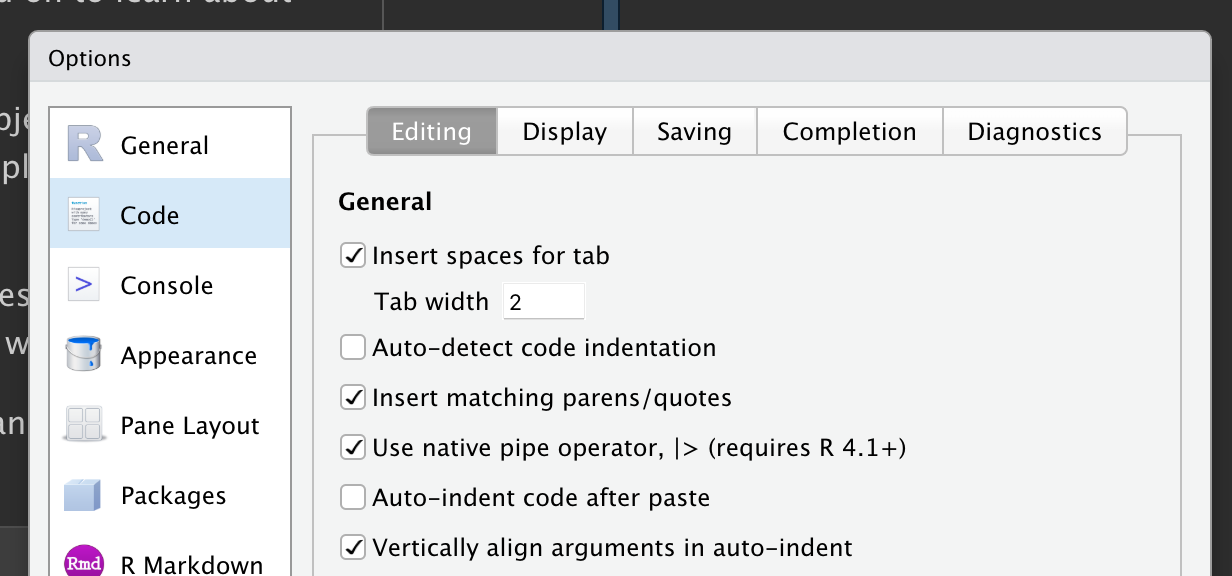
\includegraphics[width=2.05in,height=\textheight]{screenshots/rstudio-pipe-options.png}

}

\caption{\label{fig-pipe-options}To insert
\texttt{\textbar{}\textgreater{}}, make sure the ``Use native pipe
operator'' option is checked.}

\end{figure}%

\begin{tcolorbox}[enhanced jigsaw, colbacktitle=quarto-callout-note-color!10!white, breakable, opacityback=0, title=\textcolor{quarto-callout-note-color}{\faInfo}\hspace{0.5em}{Magrittr}, toprule=.15mm, leftrule=.75mm, colback=white, coltitle=black, rightrule=.15mm, opacitybacktitle=0.6, titlerule=0mm, arc=.35mm, bottomtitle=1mm, colframe=quarto-callout-note-color-frame, toptitle=1mm, bottomrule=.15mm, left=2mm]

如果您已经使用了一段时间的tidyverse,那么你可能对magrittr包提供的\%\textgreater\%管道很熟悉。\textbf{m}
\textbf{agrittr}包包含在tidyverse中,所以你可以在加载tidyverse时使用\%\textgreater\%:

\begin{Shaded}
\begin{Highlighting}[]
\FunctionTok{library}\NormalTok{(tidyverse)}

\NormalTok{mtcars }\SpecialCharTok{\%\textgreater{}\%} 
  \FunctionTok{group\_by}\NormalTok{(cyl) }\SpecialCharTok{\%\textgreater{}\%}
  \FunctionTok{summarize}\NormalTok{(}\AttributeTok{n =} \FunctionTok{n}\NormalTok{())}
\end{Highlighting}
\end{Shaded}

对于简单的情况,\textbar\textgreater 和\%\textgreater\%的行为是相同的。那
么我们为什么推荐基础管道\textbar\textgreater 呢?首 先,因为它是 R
语言的基础部分,所以你总是可以使用它,即使你没有使用 tidyverse。其
次,\textbar\textgreater 比\%\textgreater\%简单得多:在\%\textgreater\%于
2014 年被发明和\textbar\textgreater 于 2021 年在 R 4.1.0
中被引入之间的这段时间里,我们对管道有了更好的理解。这
使得\textbar\textgreater 能够舍弃那些不常用且不太重要的特性。

\end{tcolorbox}

\section{分组}\label{ux5206ux7ec4}

到目前为止,你已经学习了处理行和列的函数。当
你添加了处理分组的能力时,dplyr会变得更加强大。在
本节中,我们将重点关注最重要的函数:group\_by()、summarize()和slice函数族。

\subsection{group\_by()}\label{group_by}

使用group\_by()将数据集划分为对分析有意义的组:

\begin{Shaded}
\begin{Highlighting}[]
\NormalTok{flights }\SpecialCharTok{|\textgreater{}} 
  \FunctionTok{group\_by}\NormalTok{(month)}
\CommentTok{\#\textgreater{} \# A tibble: 336,776 x 19}
\CommentTok{\#\textgreater{} \# Groups:   month [12]}
\CommentTok{\#\textgreater{}    year month   day dep\_time sched\_dep\_time dep\_delay arr\_time sched\_arr\_time}
\CommentTok{\#\textgreater{}   \textless{}int\textgreater{} \textless{}int\textgreater{} \textless{}int\textgreater{}    \textless{}int\textgreater{}          \textless{}int\textgreater{}     \textless{}dbl\textgreater{}    \textless{}int\textgreater{}          \textless{}int\textgreater{}}
\CommentTok{\#\textgreater{} 1  2013     1     1      517            515         2      830            819}
\CommentTok{\#\textgreater{} 2  2013     1     1      533            529         4      850            830}
\CommentTok{\#\textgreater{} 3  2013     1     1      542            540         2      923            850}
\CommentTok{\#\textgreater{} 4  2013     1     1      544            545        {-}1     1004           1022}
\CommentTok{\#\textgreater{} 5  2013     1     1      554            600        {-}6      812            837}
\CommentTok{\#\textgreater{} 6  2013     1     1      554            558        {-}4      740            728}
\CommentTok{\#\textgreater{} \# i 336,770 more rows}
\CommentTok{\#\textgreater{} \# i 11 more variables: arr\_delay \textless{}dbl\textgreater{}, carrier \textless{}chr\textgreater{}, flight \textless{}int\textgreater{}, ...}
\end{Highlighting}
\end{Shaded}

group\_by()并不改变数据,但如果你仔细观察输出,你会注意到输出显示它是按月``分组''(Groups:
month {[}12{]})。这 意味着后续的操作将``按月''进行。g
roup\_by()将这个分组特性(称为类)添加到数据框中,从而改变了后续应用于数据的函数的行为。

\subsection{summarize()}\label{sec-summarize}

最重要的分组操作是汇总,如果用于计算单个汇总统计量,它将数据框缩减为每个组只有一行。在
dplyr
中,这个操作是通过summarize()\footnote{如果你喜欢英式英语,也可以用\texttt{summarise()}。}完成的,如下例所示,它计算了每个月的平均离港延误时间:

\begin{Shaded}
\begin{Highlighting}[]
\NormalTok{flights }\SpecialCharTok{|\textgreater{}} 
  \FunctionTok{group\_by}\NormalTok{(month) }\SpecialCharTok{|\textgreater{}} 
  \FunctionTok{summarize}\NormalTok{(}
    \AttributeTok{avg\_delay =} \FunctionTok{mean}\NormalTok{(dep\_delay)}
\NormalTok{  )}
\CommentTok{\#\textgreater{} \# A tibble: 12 x 2}
\CommentTok{\#\textgreater{}   month avg\_delay}
\CommentTok{\#\textgreater{}   \textless{}int\textgreater{}     \textless{}dbl\textgreater{}}
\CommentTok{\#\textgreater{} 1     1        NA}
\CommentTok{\#\textgreater{} 2     2        NA}
\CommentTok{\#\textgreater{} 3     3        NA}
\CommentTok{\#\textgreater{} 4     4        NA}
\CommentTok{\#\textgreater{} 5     5        NA}
\CommentTok{\#\textgreater{} 6     6        NA}
\CommentTok{\#\textgreater{} \# i 6 more rows}
\end{Highlighting}
\end{Shaded}

哎呀!出 错了,我们所有的结果都是 NA(读作``N-A''),这是 R
中缺失值的符号。这
是因为我们观察的一些航班在延误列中有缺失数据,所以当我们将这些值包括在内计算平均值时,我们就得到了一个
NA 结果。我 们将在 章节~\ref{sec-missing-values}
部分中详细讨论缺失值,但现在我们会告诉mean()函数通过设置na.rm参数为TRUE来忽略所有缺失值:

\begin{Shaded}
\begin{Highlighting}[]
\NormalTok{flights }\SpecialCharTok{|\textgreater{}} 
  \FunctionTok{group\_by}\NormalTok{(month) }\SpecialCharTok{|\textgreater{}} 
  \FunctionTok{summarize}\NormalTok{(}
    \AttributeTok{avg\_delay =} \FunctionTok{mean}\NormalTok{(dep\_delay, }\AttributeTok{na.rm =} \ConstantTok{TRUE}\NormalTok{)}
\NormalTok{  )}
\CommentTok{\#\textgreater{} \# A tibble: 12 x 2}
\CommentTok{\#\textgreater{}   month avg\_delay}
\CommentTok{\#\textgreater{}   \textless{}int\textgreater{}     \textless{}dbl\textgreater{}}
\CommentTok{\#\textgreater{} 1     1      10.0}
\CommentTok{\#\textgreater{} 2     2      10.8}
\CommentTok{\#\textgreater{} 3     3      13.2}
\CommentTok{\#\textgreater{} 4     4      13.9}
\CommentTok{\#\textgreater{} 5     5      13.0}
\CommentTok{\#\textgreater{} 6     6      20.8}
\CommentTok{\#\textgreater{} \# i 6 more rows}
\end{Highlighting}
\end{Shaded}

你可以在单次调用summarize()时创建任意数量的汇总。在
接下来的章节中,你将学习各种有用的汇总,但其中一个非常有用的摘要是n(),它返回每个组的行数

\begin{Shaded}
\begin{Highlighting}[]
\NormalTok{flights }\SpecialCharTok{|\textgreater{}} 
  \FunctionTok{group\_by}\NormalTok{(month) }\SpecialCharTok{|\textgreater{}} 
  \FunctionTok{summarize}\NormalTok{(}
    \AttributeTok{avg\_delay =} \FunctionTok{mean}\NormalTok{(dep\_delay, }\AttributeTok{na.rm =} \ConstantTok{TRUE}\NormalTok{), }
    \AttributeTok{n =} \FunctionTok{n}\NormalTok{()}
\NormalTok{  )}
\CommentTok{\#\textgreater{} \# A tibble: 12 x 3}
\CommentTok{\#\textgreater{}   month avg\_delay     n}
\CommentTok{\#\textgreater{}   \textless{}int\textgreater{}     \textless{}dbl\textgreater{} \textless{}int\textgreater{}}
\CommentTok{\#\textgreater{} 1     1      10.0 27004}
\CommentTok{\#\textgreater{} 2     2      10.8 24951}
\CommentTok{\#\textgreater{} 3     3      13.2 28834}
\CommentTok{\#\textgreater{} 4     4      13.9 28330}
\CommentTok{\#\textgreater{} 5     5      13.0 28796}
\CommentTok{\#\textgreater{} 6     6      20.8 28243}
\CommentTok{\#\textgreater{} \# i 6 more rows}
\end{Highlighting}
\end{Shaded}

Means和counts在数据科学中可以让你走得很远,远到让你吃惊!

\subsection{slice\_ 函数族}\label{slice_-ux51fdux6570ux65cf}

有五个函数允许你方便地提取每个组中内特定行:

\begin{itemize}
\tightlist
\item
  df \textbar\textgreater{} slice\_head(n = 1) t从每个组中取第一行;
\item
  df \textbar\textgreater{} slice\_tail(n = 1) 从每个组中取最后一行;
\item
  df \textbar\textgreater{} slice\_min(x, n = 1) 取列x值最小的行;
\item
  df \textbar\textgreater{} slice\_max(x, n = 1) 取列x值最大的行;
\item
  df \textbar\textgreater{} slice\_sample(n = 1) 随机取一行。
\end{itemize}

你可以改变参数n来选择多行,或者代替n=,你可以使用prop =
0.1(例如)来选择每个组的 10\% 的行。例
如,以下代码查找每个目的地到达时延误最严重的航班:

\begin{Shaded}
\begin{Highlighting}[]
\NormalTok{flights }\SpecialCharTok{|\textgreater{}} 
  \FunctionTok{group\_by}\NormalTok{(dest) }\SpecialCharTok{|\textgreater{}} 
  \FunctionTok{slice\_max}\NormalTok{(arr\_delay, }\AttributeTok{n =} \DecValTok{1}\NormalTok{) }\SpecialCharTok{|\textgreater{}}
  \FunctionTok{relocate}\NormalTok{(dest)}
\CommentTok{\#\textgreater{} \# A tibble: 108 x 19}
\CommentTok{\#\textgreater{} \# Groups:   dest [105]}
\CommentTok{\#\textgreater{}   dest   year month   day dep\_time sched\_dep\_time dep\_delay arr\_time}
\CommentTok{\#\textgreater{}   \textless{}chr\textgreater{} \textless{}int\textgreater{} \textless{}int\textgreater{} \textless{}int\textgreater{}    \textless{}int\textgreater{}          \textless{}int\textgreater{}     \textless{}dbl\textgreater{}    \textless{}int\textgreater{}}
\CommentTok{\#\textgreater{} 1 ABQ    2013     7    22     2145           2007        98      132}
\CommentTok{\#\textgreater{} 2 ACK    2013     7    23     1139            800       219     1250}
\CommentTok{\#\textgreater{} 3 ALB    2013     1    25      123           2000       323      229}
\CommentTok{\#\textgreater{} 4 ANC    2013     8    17     1740           1625        75     2042}
\CommentTok{\#\textgreater{} 5 ATL    2013     7    22     2257            759       898      121}
\CommentTok{\#\textgreater{} 6 AUS    2013     7    10     2056           1505       351     2347}
\CommentTok{\#\textgreater{} \# i 102 more rows}
\CommentTok{\#\textgreater{} \# i 11 more variables: sched\_arr\_time \textless{}int\textgreater{}, arr\_delay \textless{}dbl\textgreater{}, ...}
\end{Highlighting}
\end{Shaded}

请注意,虽然有 105 个目的地,但我们这里得到了 108 行,这是怎么回事?s
lice\_min()和slice\_max()会保留并列的值,所以n =
1意味着给我们所有具有最高值的行。如
果你想要每个组正好一行,你可以设置with\_ties = FALSE。

这与使用summarize()计算最大延误类似,但你会得到整个对应的行(如果有并列值,则是多行),而不是单个汇总统计量。

\subsection{按多变量分组}\label{ux6309ux591aux53d8ux91cfux5206ux7ec4}

可以使用多个变量创建分组。例 如,我们可以为每个日期创建一个组。

You can create groups using more than one variable. For example, we
could make a group for each date.

\begin{Shaded}
\begin{Highlighting}[]
\NormalTok{daily }\OtherTok{\textless{}{-}}\NormalTok{ flights }\SpecialCharTok{|\textgreater{}}  
  \FunctionTok{group\_by}\NormalTok{(year, month, day)}
\NormalTok{daily}
\CommentTok{\#\textgreater{} \# A tibble: 336,776 x 19}
\CommentTok{\#\textgreater{} \# Groups:   year, month, day [365]}
\CommentTok{\#\textgreater{}    year month   day dep\_time sched\_dep\_time dep\_delay arr\_time sched\_arr\_time}
\CommentTok{\#\textgreater{}   \textless{}int\textgreater{} \textless{}int\textgreater{} \textless{}int\textgreater{}    \textless{}int\textgreater{}          \textless{}int\textgreater{}     \textless{}dbl\textgreater{}    \textless{}int\textgreater{}          \textless{}int\textgreater{}}
\CommentTok{\#\textgreater{} 1  2013     1     1      517            515         2      830            819}
\CommentTok{\#\textgreater{} 2  2013     1     1      533            529         4      850            830}
\CommentTok{\#\textgreater{} 3  2013     1     1      542            540         2      923            850}
\CommentTok{\#\textgreater{} 4  2013     1     1      544            545        {-}1     1004           1022}
\CommentTok{\#\textgreater{} 5  2013     1     1      554            600        {-}6      812            837}
\CommentTok{\#\textgreater{} 6  2013     1     1      554            558        {-}4      740            728}
\CommentTok{\#\textgreater{} \# i 336,770 more rows}
\CommentTok{\#\textgreater{} \# i 11 more variables: arr\_delay \textless{}dbl\textgreater{}, carrier \textless{}chr\textgreater{}, flight \textless{}int\textgreater{}, ...}
\end{Highlighting}
\end{Shaded}

当你在使用多个变量对 tibble
进行分组并对其进行汇总时,每个汇总都会去掉最后一个分组。事
后看来,这不是让这个函数工作的好方法,但如果不破坏现有代码就很难改变它。为
了让发生的事情变得显而易见,dplyr
显示了一条消息,告诉你如何改变这种行为:

\begin{Shaded}
\begin{Highlighting}[]
\NormalTok{daily\_flights }\OtherTok{\textless{}{-}}\NormalTok{ daily }\SpecialCharTok{|\textgreater{}} 
  \FunctionTok{summarize}\NormalTok{(}\AttributeTok{n =} \FunctionTok{n}\NormalTok{())}
\CommentTok{\#\textgreater{} \textasciigrave{}summarise()\textasciigrave{} has grouped output by \textquotesingle{}year\textquotesingle{}, \textquotesingle{}month\textquotesingle{}. You can override using}
\CommentTok{\#\textgreater{} the \textasciigrave{}.groups\textasciigrave{} argument.}
\end{Highlighting}
\end{Shaded}

如果你对这种行为感到满意,你可以明确地要求它以抑制这条消息:

\begin{Shaded}
\begin{Highlighting}[]
\NormalTok{daily\_flights }\OtherTok{\textless{}{-}}\NormalTok{ daily }\SpecialCharTok{|\textgreater{}} 
  \FunctionTok{summarize}\NormalTok{(}
    \AttributeTok{n =} \FunctionTok{n}\NormalTok{(), }
    \AttributeTok{.groups =} \StringTok{"drop\_last"}
\NormalTok{  )}
\end{Highlighting}
\end{Shaded}

或者,通过设置不同的值来改变默认行为,例如,``drop'' 删除所有分组,或者
``keep'' 保留相同的分组。

\subsection{去消分组}\label{ux53bbux6d88ux5206ux7ec4}

您可能还希望在不使用summarize()的情况下从数据框中删除分组。您
可以使用ungroup()实现这一点。

\begin{Shaded}
\begin{Highlighting}[]
\NormalTok{daily }\SpecialCharTok{|\textgreater{}} 
  \FunctionTok{ungroup}\NormalTok{()}
\CommentTok{\#\textgreater{} \# A tibble: 336,776 x 19}
\CommentTok{\#\textgreater{}    year month   day dep\_time sched\_dep\_time dep\_delay arr\_time sched\_arr\_time}
\CommentTok{\#\textgreater{}   \textless{}int\textgreater{} \textless{}int\textgreater{} \textless{}int\textgreater{}    \textless{}int\textgreater{}          \textless{}int\textgreater{}     \textless{}dbl\textgreater{}    \textless{}int\textgreater{}          \textless{}int\textgreater{}}
\CommentTok{\#\textgreater{} 1  2013     1     1      517            515         2      830            819}
\CommentTok{\#\textgreater{} 2  2013     1     1      533            529         4      850            830}
\CommentTok{\#\textgreater{} 3  2013     1     1      542            540         2      923            850}
\CommentTok{\#\textgreater{} 4  2013     1     1      544            545        {-}1     1004           1022}
\CommentTok{\#\textgreater{} 5  2013     1     1      554            600        {-}6      812            837}
\CommentTok{\#\textgreater{} 6  2013     1     1      554            558        {-}4      740            728}
\CommentTok{\#\textgreater{} \# i 336,770 more rows}
\CommentTok{\#\textgreater{} \# i 11 more variables: arr\_delay \textless{}dbl\textgreater{}, carrier \textless{}chr\textgreater{}, flight \textless{}int\textgreater{}, ...}
\end{Highlighting}
\end{Shaded}

现在让我们看看在汇总未分组的数据框时会发生什么。

\begin{Shaded}
\begin{Highlighting}[]
\NormalTok{daily }\SpecialCharTok{|\textgreater{}} 
  \FunctionTok{ungroup}\NormalTok{() }\SpecialCharTok{|\textgreater{}}
  \FunctionTok{summarize}\NormalTok{(}
    \AttributeTok{avg\_delay =} \FunctionTok{mean}\NormalTok{(dep\_delay, }\AttributeTok{na.rm =} \ConstantTok{TRUE}\NormalTok{), }
    \AttributeTok{flights =} \FunctionTok{n}\NormalTok{()}
\NormalTok{  )}
\CommentTok{\#\textgreater{} \# A tibble: 1 x 2}
\CommentTok{\#\textgreater{}   avg\_delay flights}
\CommentTok{\#\textgreater{}       \textless{}dbl\textgreater{}   \textless{}int\textgreater{}}
\CommentTok{\#\textgreater{} 1      12.6  336776}
\end{Highlighting}
\end{Shaded}

返回一行,因为dplyr将未分组数据框中的所有行视为属于一个组。

\subsection{.by}\label{by}

dplyr 1.1.0
引入了一个新的处于试验阶段的语法,用于每次操作的分组,即.by参数。g
roup\_by()和ungroup()不会被弃用,但现在你也可以在单个操作中使用.by参数进行分组:

\begin{Shaded}
\begin{Highlighting}[]
\NormalTok{flights }\SpecialCharTok{|\textgreater{}} 
  \FunctionTok{summarize}\NormalTok{(}
    \AttributeTok{delay =} \FunctionTok{mean}\NormalTok{(dep\_delay, }\AttributeTok{na.rm =} \ConstantTok{TRUE}\NormalTok{), }
    \AttributeTok{n =} \FunctionTok{n}\NormalTok{(),}
    \AttributeTok{.by =}\NormalTok{ month}
\NormalTok{  )}
\end{Highlighting}
\end{Shaded}

或者如果你想按多个变量分组:

\begin{Shaded}
\begin{Highlighting}[]
\NormalTok{flights }\SpecialCharTok{|\textgreater{}} 
  \FunctionTok{summarize}\NormalTok{(}
    \AttributeTok{delay =} \FunctionTok{mean}\NormalTok{(dep\_delay, }\AttributeTok{na.rm =} \ConstantTok{TRUE}\NormalTok{), }
    \AttributeTok{n =} \FunctionTok{n}\NormalTok{(),}
    \AttributeTok{.by =} \FunctionTok{c}\NormalTok{(origin, dest)}
\NormalTok{  )}
\end{Highlighting}
\end{Shaded}

.by与所有动词(函数)兼容,其优势在于你不需要使用.groups参数来抑制分组消息,或在完成后使用ungroup()。

我们在编写本书时,没有重点关注这种语法,因为它当时非常新。但
我们还是想提一下,因为我们认为它很有前景,并且可能会非常受欢迎。你
可以在
\href{https://www.tidyverse.org/blog/2023/02/dplyr-1-1-0-per-operation-grouping/}{dplyr
1.1.0 的博客}中了解更多关于它的信息。

\subsection{练习}\label{ux7ec3ux4e60-7}

\begin{enumerate}
\def\labelenumi{\arabic{enumi}.}
\item
  哪家航空公司的平均延误时间最长?挑
  战:你能理清机场差和航空公司差的影响吗?为 什么能/为什么不能?( 提示:
  考虑使用 flights \textbar\textgreater{} group\_by(carrier, dest)
  \textbar\textgreater{} summarize(n()))
\item
  找出从每个目的地出发延误最严重的航班;
\item
  延误情况在一天中是如何变化的?用 图表来展示你的答案;
\item
  如果你给slice\_min()及其相关函数提供负的n值会怎样?
\item
  用你刚刚学习的 dplyr 动词(函数)来解释count()做了什么。c
  ount()的sort参数有什么作用?
\item
  假设我们有以下的小数据框:

\begin{Shaded}
\begin{Highlighting}[]
\NormalTok{df }\OtherTok{\textless{}{-}} \FunctionTok{tibble}\NormalTok{(}
  \AttributeTok{x =} \DecValTok{1}\SpecialCharTok{:}\DecValTok{5}\NormalTok{,}
  \AttributeTok{y =} \FunctionTok{c}\NormalTok{(}\StringTok{"a"}\NormalTok{, }\StringTok{"b"}\NormalTok{, }\StringTok{"a"}\NormalTok{, }\StringTok{"a"}\NormalTok{, }\StringTok{"b"}\NormalTok{),}
  \AttributeTok{z =} \FunctionTok{c}\NormalTok{(}\StringTok{"K"}\NormalTok{, }\StringTok{"K"}\NormalTok{, }\StringTok{"L"}\NormalTok{, }\StringTok{"L"}\NormalTok{, }\StringTok{"K"}\NormalTok{)}
\NormalTok{)}
\end{Highlighting}
\end{Shaded}

  \begin{enumerate}
  \def\labelenumii{\alph{enumii}.}
  \item
    写下你认为的输出是什么样子,然后检查是否正确,并描述group\_by()的作用。

\begin{Shaded}
\begin{Highlighting}[]
\NormalTok{df }\SpecialCharTok{|\textgreater{}}
  \FunctionTok{group\_by}\NormalTok{(y)}
\end{Highlighting}
\end{Shaded}
  \item
    写下你认为的输出是什么样子,然后检查你是否正确,并描述arrange()的作用。同
    时评论一下它与(a)部分中的group\_by()有什么不同。

\begin{Shaded}
\begin{Highlighting}[]
\NormalTok{df }\SpecialCharTok{|\textgreater{}}
  \FunctionTok{arrange}\NormalTok{(y)}
\end{Highlighting}
\end{Shaded}
  \item
    写下你认为的输出是什么样子,然后检查你是否正确,并描述管道的功能。

\begin{Shaded}
\begin{Highlighting}[]
\NormalTok{df }\SpecialCharTok{|\textgreater{}}
  \FunctionTok{group\_by}\NormalTok{(y) }\SpecialCharTok{|\textgreater{}}
  \FunctionTok{summarize}\NormalTok{(}\AttributeTok{mean\_x =} \FunctionTok{mean}\NormalTok{(x))}
\end{Highlighting}
\end{Shaded}
  \item
    写下你认为的输出是什么样子,然后检查你是否正确,并描述管道的功能。然
    后对信息内容进行评论。

\begin{Shaded}
\begin{Highlighting}[]
\NormalTok{df }\SpecialCharTok{|\textgreater{}}
  \FunctionTok{group\_by}\NormalTok{(y, z) }\SpecialCharTok{|\textgreater{}}
  \FunctionTok{summarize}\NormalTok{(}\AttributeTok{mean\_x =} \FunctionTok{mean}\NormalTok{(x))}
\end{Highlighting}
\end{Shaded}
  \item
    写下你认为的输出是什么样子,然后检查你是否正确,并描述管道的功能。与
    (d)部分中的输出有何不同?

\begin{Shaded}
\begin{Highlighting}[]
\NormalTok{df }\SpecialCharTok{|\textgreater{}}
  \FunctionTok{group\_by}\NormalTok{(y, z) }\SpecialCharTok{|\textgreater{}}
  \FunctionTok{summarize}\NormalTok{(}\AttributeTok{mean\_x =} \FunctionTok{mean}\NormalTok{(x), }\AttributeTok{.groups =} \StringTok{"drop"}\NormalTok{)}
\end{Highlighting}
\end{Shaded}
  \item
    写下你认为的输出是什么样子,然后检查你是否正确,并描述每个管道的作用。两
    个管道的输出有什么不同?

\begin{Shaded}
\begin{Highlighting}[]
\NormalTok{df }\SpecialCharTok{|\textgreater{}}
  \FunctionTok{group\_by}\NormalTok{(y, z) }\SpecialCharTok{|\textgreater{}}
  \FunctionTok{summarize}\NormalTok{(}\AttributeTok{mean\_x =} \FunctionTok{mean}\NormalTok{(x))}

\NormalTok{df }\SpecialCharTok{|\textgreater{}}
  \FunctionTok{group\_by}\NormalTok{(y, z) }\SpecialCharTok{|\textgreater{}}
  \FunctionTok{mutate}\NormalTok{(}\AttributeTok{mean\_x =} \FunctionTok{mean}\NormalTok{(x))}
\end{Highlighting}
\end{Shaded}
  \end{enumerate}
\end{enumerate}

\section{案例研究: 汇总数据和样本量}\label{sec-sample-size}

无论何时进行数据汇总,包含计数(n())总是一个好主意。这
样可以确保你不是基于很少量的数据来得出结论。我
们将使用\textbf{Lahman}包中的棒球数据来演示这一点。具
体来说,我们将比较球员击球成功(H)的次数与尝试击球(AB)的次数之间的比例:

\begin{Shaded}
\begin{Highlighting}[]
\NormalTok{batters }\OtherTok{\textless{}{-}}\NormalTok{ Lahman}\SpecialCharTok{::}\NormalTok{Batting }\SpecialCharTok{|\textgreater{}} 
  \FunctionTok{group\_by}\NormalTok{(playerID) }\SpecialCharTok{|\textgreater{}} 
  \FunctionTok{summarize}\NormalTok{(}
    \AttributeTok{performance =} \FunctionTok{sum}\NormalTok{(H, }\AttributeTok{na.rm =} \ConstantTok{TRUE}\NormalTok{) }\SpecialCharTok{/} \FunctionTok{sum}\NormalTok{(AB, }\AttributeTok{na.rm =} \ConstantTok{TRUE}\NormalTok{),}
    \AttributeTok{n =} \FunctionTok{sum}\NormalTok{(AB, }\AttributeTok{na.rm =} \ConstantTok{TRUE}\NormalTok{)}
\NormalTok{  )}
\NormalTok{batters}
\CommentTok{\#\textgreater{} \# A tibble: 20,469 x 3}
\CommentTok{\#\textgreater{}   playerID  performance     n}
\CommentTok{\#\textgreater{}   \textless{}chr\textgreater{}           \textless{}dbl\textgreater{} \textless{}int\textgreater{}}
\CommentTok{\#\textgreater{} 1 aardsda01      0          4}
\CommentTok{\#\textgreater{} 2 aaronha01      0.305  12364}
\CommentTok{\#\textgreater{} 3 aaronto01      0.229    944}
\CommentTok{\#\textgreater{} 4 aasedo01       0          5}
\CommentTok{\#\textgreater{} 5 abadan01       0.0952    21}
\CommentTok{\#\textgreater{} 6 abadfe01       0.111      9}
\CommentTok{\#\textgreater{} \# i 20,463 more rows}
\end{Highlighting}
\end{Shaded}

当我们绘制击球手的技巧(通过击球率来衡量,即performance)与击球机会的数量(通过击球次数来衡量,即n)之间的关系时,你会看到两种模式:

\begin{enumerate}
\def\labelenumi{\arabic{enumi}.}
\tightlist
\item
  击球次数较少的球员之间的技巧差异更大。这种图的形状非常典型:每当你绘制平均值(或其他汇总统计量)与组大小时,你会看到随着样本量的增加,变异程度会降低\footnote{大数定律}。
\item
  技巧(performance)与击球机会(n)之间存在正相关关系,因为球队希望给他们的最佳击球手最多的击球机会。
\end{enumerate}

\begin{Shaded}
\begin{Highlighting}[]
\NormalTok{batters }\SpecialCharTok{|\textgreater{}} 
  \FunctionTok{filter}\NormalTok{(n }\SpecialCharTok{\textgreater{}} \DecValTok{100}\NormalTok{) }\SpecialCharTok{|\textgreater{}} 
  \FunctionTok{ggplot}\NormalTok{(}\FunctionTok{aes}\NormalTok{(}\AttributeTok{x =}\NormalTok{ n, }\AttributeTok{y =}\NormalTok{ performance)) }\SpecialCharTok{+}
  \FunctionTok{geom\_point}\NormalTok{(}\AttributeTok{alpha =} \DecValTok{1} \SpecialCharTok{/} \DecValTok{10}\NormalTok{) }\SpecialCharTok{+} 
  \FunctionTok{geom\_smooth}\NormalTok{(}\AttributeTok{se =} \ConstantTok{FALSE}\NormalTok{)}
\end{Highlighting}
\end{Shaded}

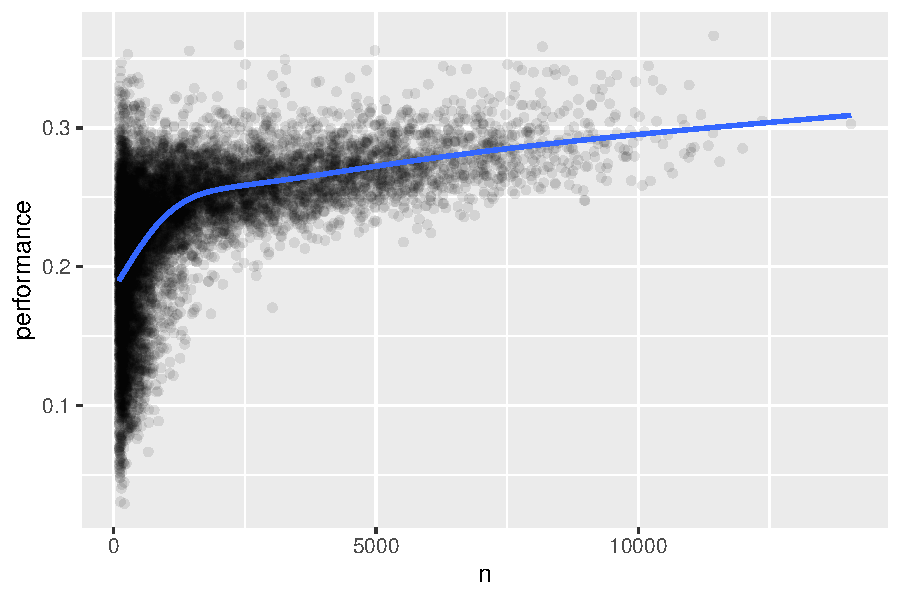
\includegraphics[width=18.75in,height=\textheight]{data-transform_files/figure-pdf/unnamed-chunk-58-1.pdf}

请注意将ggplot2和dplyr结合使用的便捷模式。你
只需要记住在数据集处理时使用\textbar\textgreater,而在向你的图添加图层时使用+。

这对于排名也有重要的影响。如
果你只是简单地根据desc(performance)进行排序,那么显然击球率最好的人是那些尝试击球次数很少但碰巧击中的人,他们不一定是技术最熟练的球员:

\begin{Shaded}
\begin{Highlighting}[]
\NormalTok{batters }\SpecialCharTok{|\textgreater{}} 
  \FunctionTok{arrange}\NormalTok{(}\FunctionTok{desc}\NormalTok{(performance))}
\CommentTok{\#\textgreater{} \# A tibble: 20,469 x 3}
\CommentTok{\#\textgreater{}   playerID  performance     n}
\CommentTok{\#\textgreater{}   \textless{}chr\textgreater{}           \textless{}dbl\textgreater{} \textless{}int\textgreater{}}
\CommentTok{\#\textgreater{} 1 abramge01           1     1}
\CommentTok{\#\textgreater{} 2 alberan01           1     1}
\CommentTok{\#\textgreater{} 3 banisje01           1     1}
\CommentTok{\#\textgreater{} 4 bartocl01           1     1}
\CommentTok{\#\textgreater{} 5 bassdo01            1     1}
\CommentTok{\#\textgreater{} 6 birasst01           1     2}
\CommentTok{\#\textgreater{} \# i 20,463 more rows}
\end{Highlighting}
\end{Shaded}

关于这个问题及其解决方法,你可以在以下网址找到很好的解释:
\url{http://varianceexplained.org/r/empirical_bayes_baseball/} 和
\url{https://www.evanmiller.org/how-not-to-sort-by-average-rating.html}.

\section{小结}\label{ux5c0fux7ed3-2}

在本章中,你学习了dplyr为处理数据框提供的工具。这
些工具大致分为三类:操作行的工具(如\texttt{filter()}和\texttt{arrange()}),操作列的工具(如\texttt{select()}和\texttt{mutate()}),以及操作组的工具(如\texttt{group\_by()}和\texttt{summarize()})。在
本章中,我们专注于这些``整个数据框''的工具,但你还没有深入了解可以使用单个变量做什么。我
们将在本书的转换部分回到这个问题,其中每一章都将为你提供特定类型变量的工具。

在下一章中,我们将回到工作流程,讨论代码风格的重要性,保持您的代码组织良好,以便你和他人能够轻松阅读和理解你的代码。

\chapter{工作流程: 代码风格}\label{sec-workflow-style}

良好的编码风格就像正确的标点符号:没有它也能写代码,但它确实能让事情变得更易于阅读。即
使作为一名非常新的程序员,养成好的代码风格也是一个好主意。使
用一致的代码风格可以让他人(包括未来的你)更容易读懂你的工作,这在你需要他人帮助时变得尤为重要。本
章将介绍\href{https://style.tidyverse.org}{tidyverse风格指南}的最重要内容,该指南在本书中贯穿始终。

刚开始为代码设置样式可能会觉得有些乏味,但如果你坚持练习,它很快就会成为你的第二天性。此
外,还有一些很棒的工具可以快速重新格式化现有的代码,比如Lorenz
Walthert的\href{https://styler.r-lib.org}{\textbf{styler}}包。一
旦你使用\texttt{install.packages("styler")}安装了这个包,一个简单的使用方法是通过RStudio的命令面板。命
令面板允许你使用任何内置的RStudio命令以及由包提供的许多插件。通
过按Cmd/Ctrl + Shift +
P打开面板,然后输入``styler''来查看styler提供的所有快捷键,图~\ref{fig-styler}
展示了结果。

\begin{figure}

\centering{

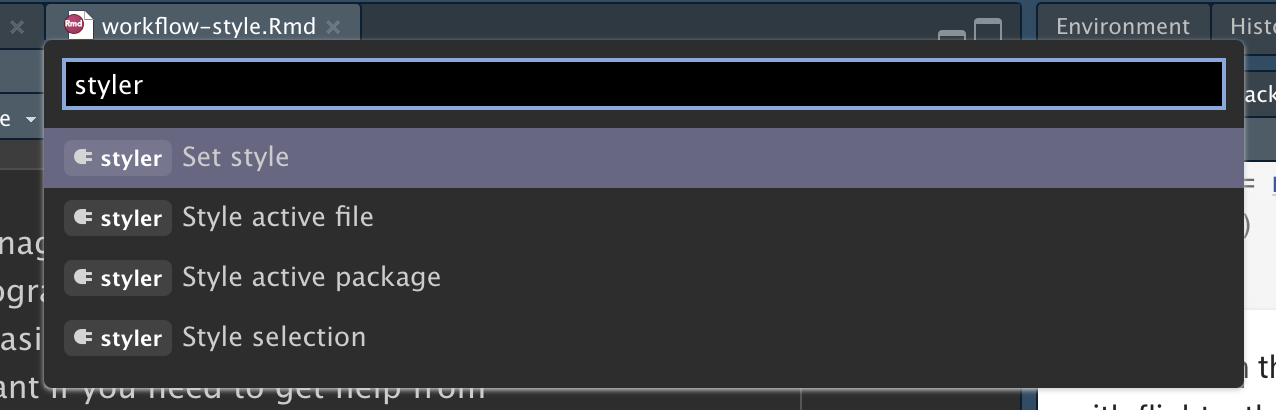
\includegraphics[width=2.13in,height=\textheight]{screenshots/rstudio-palette.png}

}

\caption{\label{fig-styler}RStudio's command palette makes it easy to
access every RStudio command using only the keyboard.}

\end{figure}%

在本章中,我们将使用tidyverse和nycflights13包作为代码示例。

\begin{Shaded}
\begin{Highlighting}[]
\FunctionTok{library}\NormalTok{(tidyverse)}
\FunctionTok{library}\NormalTok{(nycflights13)}
\end{Highlighting}
\end{Shaded}

\section{名称}\label{ux540dux79f0}

我们在@sec-whats-in-a-name 简要地讨论了名称。请
记住,变量名(通过\texttt{\textless{}-}和\texttt{mutate()}创建的)应该只使用小写字母、数字和\texttt{\_}。使
用\texttt{\_}来分隔名称中的单词。

\begin{Shaded}
\begin{Highlighting}[]
\CommentTok{\# Strive for:}
\NormalTok{short\_flights }\OtherTok{\textless{}{-}}\NormalTok{ flights }\SpecialCharTok{|\textgreater{}} \FunctionTok{filter}\NormalTok{(air\_time }\SpecialCharTok{\textless{}} \DecValTok{60}\NormalTok{)}

\CommentTok{\# Avoid:}
\NormalTok{SHORTFLIGHTS }\OtherTok{\textless{}{-}}\NormalTok{ flights }\SpecialCharTok{|\textgreater{}} \FunctionTok{filter}\NormalTok{(air\_time }\SpecialCharTok{\textless{}} \DecValTok{60}\NormalTok{)}
\end{Highlighting}
\end{Shaded}

作为一条通用的经验法则,最好选择长而描述性强的名称,这样更容易理解,而不是快速输入的简洁名称。在
编写代码时,短名称节省的时间相对较少(特别是当自动补全功能帮助你完成输入时),但当你回到旧代码并被迫猜测一个晦涩的缩写时,这可能会很耗时。

如果你有一组与相关事物相关的名称,请尽量保持一致。当
你忘记之前的约定时,不一致性很容易产生,所以如果你必须回去重命名事物,也不要感到难过。一
般来说,如果你有一组变量是某个主题的变体,最好给它们一个共同的前缀而不是共同的后缀,因为自动补全在变量的开头效果最好。

\section{空格}\label{ux7a7aux683c}

在除\texttt{\^{}}以外的数学运算符(即\texttt{-}、\texttt{==}、\texttt{\textless{}}、\ldots)以及赋值运算符(\texttt{\textless{}-})的两侧加上空格。

\begin{Shaded}
\begin{Highlighting}[]
\CommentTok{\# Strive for}
\NormalTok{z }\OtherTok{\textless{}{-}}\NormalTok{ (a }\SpecialCharTok{+}\NormalTok{ b)}\SpecialCharTok{\^{}}\DecValTok{2} \SpecialCharTok{/}\NormalTok{ d}

\CommentTok{\# Avoid}
\NormalTok{z}\OtherTok{\textless{}{-}}\NormalTok{( a }\SpecialCharTok{+}\NormalTok{ b ) }\SpecialCharTok{\^{}} \DecValTok{2}\SpecialCharTok{/}\NormalTok{d}
\end{Highlighting}
\end{Shaded}

对于常规函数调用,不要在圆括号内或圆括号外放空格。总
是在逗号后面加一个空格,就像在标准英语中一样。

\begin{Shaded}
\begin{Highlighting}[]
\CommentTok{\# Strive for}
\FunctionTok{mean}\NormalTok{(x, }\AttributeTok{na.rm =} \ConstantTok{TRUE}\NormalTok{)}

\CommentTok{\# Avoid}
\FunctionTok{mean}\NormalTok{ (x ,}\AttributeTok{na.rm=}\ConstantTok{TRUE}\NormalTok{)}
\end{Highlighting}
\end{Shaded}

如果可以提高对齐效果,可以添加额外的空格。例
如,如果要在mutate()中创建多个变量,则可能需要添加空格,以便所有的\texttt{=}对齐\footnote{由于\texttt{dep\_time}是\texttt{HMM}或\texttt{HHMM}格式,因此我们使用整数除法(\texttt{\%/\%})来获得小时,使用余数(也称为取模,\texttt{\%\%})来获得分钟。}。
这会使得浏览代码更容易。

\begin{Shaded}
\begin{Highlighting}[]
\NormalTok{flights }\SpecialCharTok{|\textgreater{}} 
  \FunctionTok{mutate}\NormalTok{(}
    \AttributeTok{speed      =}\NormalTok{ distance }\SpecialCharTok{/}\NormalTok{ air\_time,}
    \AttributeTok{dep\_hour   =}\NormalTok{ dep\_time }\SpecialCharTok{\%/\%} \DecValTok{100}\NormalTok{,}
    \AttributeTok{dep\_minute =}\NormalTok{ dep\_time }\SpecialCharTok{\%\%}  \DecValTok{100}
\NormalTok{  )}
\end{Highlighting}
\end{Shaded}

\section{管道}\label{sec-pipes}

\texttt{\textbar{}\textgreater{}}前面应该始终有一个空格,并且通常应该是行的最后一个元素。这
样做可以更容易地添加新步骤、重新排列现有步骤、修改步骤中的元素,并通过浏览左侧的动词(函数)来获得一个全局视角。

\begin{Shaded}
\begin{Highlighting}[]
\CommentTok{\# Strive for }
\NormalTok{flights }\SpecialCharTok{|\textgreater{}}  
  \FunctionTok{filter}\NormalTok{(}\SpecialCharTok{!}\FunctionTok{is.na}\NormalTok{(arr\_delay), }\SpecialCharTok{!}\FunctionTok{is.na}\NormalTok{(tailnum)) }\SpecialCharTok{|\textgreater{}} 
  \FunctionTok{count}\NormalTok{(dest)}

\CommentTok{\# Avoid}
\NormalTok{flights}\SpecialCharTok{|\textgreater{}}\FunctionTok{filter}\NormalTok{(}\SpecialCharTok{!}\FunctionTok{is.na}\NormalTok{(arr\_delay), }\SpecialCharTok{!}\FunctionTok{is.na}\NormalTok{(tailnum))}\SpecialCharTok{|\textgreater{}}\FunctionTok{count}\NormalTok{(dest)}
\end{Highlighting}
\end{Shaded}

如果你正在使用管道传递数据的函数具有被命名的参数(如\texttt{mutate()}或\texttt{summarize()}),请将每个参数放在新行上。如
果函数没有命名参数(如\texttt{select()}或\texttt{filter()}),则除非参数过长无法放在一行中,否则将所有内容放在一行上。在
参数过长的情况下,你应该将每个参数放在自己的行上。

\begin{Shaded}
\begin{Highlighting}[]
\CommentTok{\# Strive for}
\NormalTok{flights }\SpecialCharTok{|\textgreater{}}  
  \FunctionTok{group\_by}\NormalTok{(tailnum) }\SpecialCharTok{|\textgreater{}} 
  \FunctionTok{summarize}\NormalTok{(}
    \AttributeTok{delay =} \FunctionTok{mean}\NormalTok{(arr\_delay, }\AttributeTok{na.rm =} \ConstantTok{TRUE}\NormalTok{),}
    \AttributeTok{n =} \FunctionTok{n}\NormalTok{()}
\NormalTok{  )}

\CommentTok{\# Avoid}
\NormalTok{flights }\SpecialCharTok{|\textgreater{}}
  \FunctionTok{group\_by}\NormalTok{(}
\NormalTok{    tailnum}
\NormalTok{  ) }\SpecialCharTok{|\textgreater{}} 
  \FunctionTok{summarize}\NormalTok{(}\AttributeTok{delay =} \FunctionTok{mean}\NormalTok{(arr\_delay, }\AttributeTok{na.rm =} \ConstantTok{TRUE}\NormalTok{), }\AttributeTok{n =} \FunctionTok{n}\NormalTok{())}
\end{Highlighting}
\end{Shaded}

在管道的第一步之后,将每行缩进两个空格。在
\texttt{\textbar{}\textgreater{}}后面的换行后,RStudio会自动为你添加空格。如
果你将每个参数放在单独的一行上,则再缩进两个空格。确
保\texttt{)}单独放在一行上,并且不缩进,以匹配函数名的水平位置。

\begin{Shaded}
\begin{Highlighting}[]
\CommentTok{\# Strive for }
\NormalTok{flights }\SpecialCharTok{|\textgreater{}}  
  \FunctionTok{group\_by}\NormalTok{(tailnum) }\SpecialCharTok{|\textgreater{}} 
  \FunctionTok{summarize}\NormalTok{(}
    \AttributeTok{delay =} \FunctionTok{mean}\NormalTok{(arr\_delay, }\AttributeTok{na.rm =} \ConstantTok{TRUE}\NormalTok{),}
    \AttributeTok{n =} \FunctionTok{n}\NormalTok{()}
\NormalTok{  )}

\CommentTok{\# Avoid}
\NormalTok{flights}\SpecialCharTok{|\textgreater{}}
  \FunctionTok{group\_by}\NormalTok{(tailnum) }\SpecialCharTok{|\textgreater{}} 
  \FunctionTok{summarize}\NormalTok{(}
             \AttributeTok{delay =} \FunctionTok{mean}\NormalTok{(arr\_delay, }\AttributeTok{na.rm =} \ConstantTok{TRUE}\NormalTok{), }
             \AttributeTok{n =} \FunctionTok{n}\NormalTok{()}
\NormalTok{           )}

\CommentTok{\# Avoid}
\NormalTok{flights}\SpecialCharTok{|\textgreater{}}
  \FunctionTok{group\_by}\NormalTok{(tailnum) }\SpecialCharTok{|\textgreater{}} 
  \FunctionTok{summarize}\NormalTok{(}
  \AttributeTok{delay =} \FunctionTok{mean}\NormalTok{(arr\_delay, }\AttributeTok{na.rm =} \ConstantTok{TRUE}\NormalTok{), }
  \AttributeTok{n =} \FunctionTok{n}\NormalTok{()}
\NormalTok{  )}
\end{Highlighting}
\end{Shaded}

如果你的管道可以很容易地放在一行上,那么忽略一些规则是可以的。但
根据我们的共同经验,简短的代码片段经常会变得更长,所以通常一开始就使用所有你需要的垂直空间会在长远上节省时间。

\begin{Shaded}
\begin{Highlighting}[]
\CommentTok{\# This fits compactly on one line}
\NormalTok{df }\SpecialCharTok{|\textgreater{}} \FunctionTok{mutate}\NormalTok{(}\AttributeTok{y =}\NormalTok{ x }\SpecialCharTok{+} \DecValTok{1}\NormalTok{)}

\CommentTok{\# While this takes up 4x as many lines, it\textquotesingle{}s easily extended to }
\CommentTok{\# more variables and more steps in the future}
\NormalTok{df }\SpecialCharTok{|\textgreater{}} 
  \FunctionTok{mutate}\NormalTok{(}
    \AttributeTok{y =}\NormalTok{ x }\SpecialCharTok{+} \DecValTok{1}
\NormalTok{  )}
\end{Highlighting}
\end{Shaded}

最后,要警惕编写非常长的管道,比如超过10-15行的管道。尝
试将它们分解成更小的子任务,并为每个任务赋予一个信息性强的名称。这
些名称将帮助读者了解正在发生的事情,并更容易地检查中间结果是否符合预期。只
要你能为某个事物赋予一个信息性强的名称,你就应该这样做,例如当你从根本上改变数据的结构时,例如在透视或汇总之后。不
要期望第一次就能做对!这
意味着,如果中间状态可以得到好的名称,就应该拆分长的管道。

\section{ggplot2}\label{ggplot2}

适用于管道的基本规则也适用于ggplot2,对待\texttt{+}就像对待\texttt{\textbar{}\textgreater{}}一样。

\begin{Shaded}
\begin{Highlighting}[]
\NormalTok{flights }\SpecialCharTok{|\textgreater{}} 
  \FunctionTok{group\_by}\NormalTok{(month) }\SpecialCharTok{|\textgreater{}} 
  \FunctionTok{summarize}\NormalTok{(}
    \AttributeTok{delay =} \FunctionTok{mean}\NormalTok{(arr\_delay, }\AttributeTok{na.rm =} \ConstantTok{TRUE}\NormalTok{)}
\NormalTok{  ) }\SpecialCharTok{|\textgreater{}} 
  \FunctionTok{ggplot}\NormalTok{(}\FunctionTok{aes}\NormalTok{(}\AttributeTok{x =}\NormalTok{ month, }\AttributeTok{y =}\NormalTok{ delay)) }\SpecialCharTok{+}
  \FunctionTok{geom\_point}\NormalTok{() }\SpecialCharTok{+} 
  \FunctionTok{geom\_line}\NormalTok{()}
\end{Highlighting}
\end{Shaded}

同样,如果你不能将函数的所有参数放在一行中,请将每个参数放在单独的一行中:

\begin{Shaded}
\begin{Highlighting}[]
\NormalTok{flights }\SpecialCharTok{|\textgreater{}} 
  \FunctionTok{group\_by}\NormalTok{(dest) }\SpecialCharTok{|\textgreater{}} 
  \FunctionTok{summarize}\NormalTok{(}
    \AttributeTok{distance =} \FunctionTok{mean}\NormalTok{(distance),}
    \AttributeTok{speed =} \FunctionTok{mean}\NormalTok{(distance }\SpecialCharTok{/}\NormalTok{ air\_time, }\AttributeTok{na.rm =} \ConstantTok{TRUE}\NormalTok{)}
\NormalTok{  ) }\SpecialCharTok{|\textgreater{}} 
  \FunctionTok{ggplot}\NormalTok{(}\FunctionTok{aes}\NormalTok{(}\AttributeTok{x =}\NormalTok{ distance, }\AttributeTok{y =}\NormalTok{ speed)) }\SpecialCharTok{+}
  \FunctionTok{geom\_smooth}\NormalTok{(}
    \AttributeTok{method =} \StringTok{"loess"}\NormalTok{,}
    \AttributeTok{span =} \FloatTok{0.5}\NormalTok{,}
    \AttributeTok{se =} \ConstantTok{FALSE}\NormalTok{, }
    \AttributeTok{color =} \StringTok{"white"}\NormalTok{, }
    \AttributeTok{linewidth =} \DecValTok{4}
\NormalTok{  ) }\SpecialCharTok{+}
  \FunctionTok{geom\_point}\NormalTok{()}
\end{Highlighting}
\end{Shaded}

注意从 \texttt{\textbar{}\textgreater{}} 到 \texttt{+} 的转换。我
们希望这种转换是不必要的,但不幸的是,ggplot2 是在管道发明之前编写的。

\section{分段注释}\label{ux5206ux6bb5ux6ce8ux91ca}

随着你的脚本变长,你可以使用分段注释(sectioning
comments)将文件分解成可管理的片段:

\begin{Shaded}
\begin{Highlighting}[]
\CommentTok{\# Load data {-}{-}{-}{-}{-}{-}{-}{-}{-}{-}{-}{-}{-}{-}{-}{-}{-}{-}{-}{-}{-}{-}{-}{-}{-}{-}{-}{-}{-}{-}{-}{-}{-}{-}{-}{-}{-}{-}}

\CommentTok{\# Plot data {-}{-}{-}{-}{-}{-}{-}{-}{-}{-}{-}{-}{-}{-}{-}{-}{-}{-}{-}{-}{-}{-}{-}{-}{-}{-}{-}{-}{-}{-}{-}{-}{-}{-}{-}{-}{-}{-}}
\end{Highlighting}
\end{Shaded}

RStudio提供了一个快捷键来创建这些标题(Cmd/Ctrl Shift
R),并将它们显示在编辑器左下角的代码导航下拉菜单中,如
图~\ref{fig-rstudio-sections} 所示。

\begin{figure}

\centering{

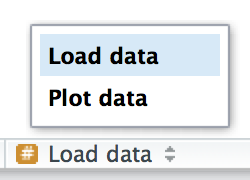
\includegraphics[width=0.42in,height=\textheight]{screenshots/rstudio-nav.png}

}

\caption{\label{fig-rstudio-sections}After adding sectioning comments to
your script, you can easily navigate to them using the code navigation
tool in the bottom-left of the script editor.}

\end{figure}%

\section{练习}\label{ux7ec3ux4e60-8}

\begin{enumerate}
\def\labelenumi{\arabic{enumi}.}
\item
  按照上面的指南重新设计以下管道的样式。

\begin{Shaded}
\begin{Highlighting}[]
\NormalTok{flights}\SpecialCharTok{|\textgreater{}}\FunctionTok{filter}\NormalTok{(dest}\SpecialCharTok{==}\StringTok{"IAH"}\NormalTok{)}\SpecialCharTok{|\textgreater{}}\FunctionTok{group\_by}\NormalTok{(year,month,day)}\SpecialCharTok{|\textgreater{}}\FunctionTok{summarize}\NormalTok{(}\AttributeTok{n=}\FunctionTok{n}\NormalTok{(),}
\AttributeTok{delay=}\FunctionTok{mean}\NormalTok{(arr\_delay,}\AttributeTok{na.rm=}\ConstantTok{TRUE}\NormalTok{))}\SpecialCharTok{|\textgreater{}}\FunctionTok{filter}\NormalTok{(n}\SpecialCharTok{\textgreater{}}\DecValTok{10}\NormalTok{)}

\NormalTok{flights}\SpecialCharTok{|\textgreater{}}\FunctionTok{filter}\NormalTok{(carrier}\SpecialCharTok{==}\StringTok{"UA"}\NormalTok{,dest}\SpecialCharTok{\%in\%}\FunctionTok{c}\NormalTok{(}\StringTok{"IAH"}\NormalTok{,}\StringTok{"HOU"}\NormalTok{),sched\_dep\_time}\SpecialCharTok{\textgreater{}}
\DecValTok{0900}\NormalTok{,sched\_arr\_time}\SpecialCharTok{\textless{}}\DecValTok{2000}\NormalTok{)}\SpecialCharTok{|\textgreater{}}\FunctionTok{group\_by}\NormalTok{(flight)}\SpecialCharTok{|\textgreater{}}\FunctionTok{summarize}\NormalTok{(}\AttributeTok{delay=}\FunctionTok{mean}\NormalTok{(}
\NormalTok{arr\_delay,}\AttributeTok{na.rm=}\ConstantTok{TRUE}\NormalTok{),}\AttributeTok{cancelled=}\FunctionTok{sum}\NormalTok{(}\FunctionTok{is.na}\NormalTok{(arr\_delay)),}\AttributeTok{n=}\FunctionTok{n}\NormalTok{())}\SpecialCharTok{|\textgreater{}}\FunctionTok{filter}\NormalTok{(n}\SpecialCharTok{\textgreater{}}\DecValTok{10}\NormalTok{)}
\end{Highlighting}
\end{Shaded}
\end{enumerate}

\section{小结}\label{ux5c0fux7ed3-3}

在本章中,你学习了代码风格最重要的原则。这
些原则一开始可能感觉像是一套任意的规则(因为它们确实是),但随着时间的推移,当你编写更多的代码并与更多的人分享代码时,你会看到一致的样式是多么重要。别
忘了styler包,它是快速提高样式不佳的代码质量的绝佳方式。

在下一章中,我们将回到数据科学工具,学习整理数据。整
理数据是一种组织数据框的一致方式,它在tidyverse中得到了广泛应用。这
种一致性让你的生活变得更加容易,因为一旦你有了整洁的数据,它就可以与绝大多数tidyverse函数一起工作。当
然,生活从来都不容易,你在实际中遇到的大多数数据集都不会是整洁的。所
以,我们还将教你如何使用tidyr包来整理你的不整洁的数据。

\chapter{数据整理}\label{sec-data-tidy}

\section{引言}\label{ux5f15ux8a00-2}

\begin{quote}
``幸福的家庭都是相似的;每个不幸的家庭各有各的不幸。''\\
--- 列夫·托尔斯泰
\end{quote}

\begin{quote}
``整洁的数据集都是相似的,但每个混乱的数据集各有各的混乱方式。''\\
--- 哈德利·威克汉姆
\end{quote}

在本章中,你将学习一种在R中组织数据的一致方法,即利用一种被称为整齐数据(tidy
data)的系统。将
数据整理成这种格式需要一些前期工作,但从长远来看,这些工作是值得的。一
旦你有了整齐的数据和tidyverse包提供的整理工具,你将花费更少的时间将数据从一种表现形式转换为另一种表现形式,从而让你有更多的时间投入到你关心的数据问题上。

在本章中,你将首先学习整齐数据的定义,并将其应用于一个简单的示例数据集。然
后,我们将深入探讨用于整理数据的主要工具:数据重塑(data
pivoting),数据透视允许你改变数据的格式而不改变任何值。

\subsection{必要条件}\label{ux5fc5ux8981ux6761ux4ef6-2}

本章将重点介绍\texttt{tidyr},它提供了一系列工具来帮助整理混乱的数据集,是tidyverse的一个成员。

\begin{Shaded}
\begin{Highlighting}[]
\FunctionTok{library}\NormalTok{(tidyverse)}
\end{Highlighting}
\end{Shaded}

从本章开始,我们将阻止\texttt{library(tidyverse)}的加载消息。

\section{整齐数据}\label{sec-tidy-data}

你可以用多种方式表示相同的基础数据。下
面的例子展示了以三种不同的方式组织的同一数据。每
个数据集都显示了四个变量的相同值:国家(\emph{country})、年份(\emph{year})、人口(\emph{population})和记录在案的结核病(tuberculosis,TB)病例数(\emph{cases}),但每个数据集都以不同的方式组织这些值。

\begin{Shaded}
\begin{Highlighting}[]
\NormalTok{table1}
\CommentTok{\#\textgreater{} \# A tibble: 6 x 4}
\CommentTok{\#\textgreater{}   country      year  cases population}
\CommentTok{\#\textgreater{}   \textless{}chr\textgreater{}       \textless{}dbl\textgreater{}  \textless{}dbl\textgreater{}      \textless{}dbl\textgreater{}}
\CommentTok{\#\textgreater{} 1 Afghanistan  1999    745   19987071}
\CommentTok{\#\textgreater{} 2 Afghanistan  2000   2666   20595360}
\CommentTok{\#\textgreater{} 3 Brazil       1999  37737  172006362}
\CommentTok{\#\textgreater{} 4 Brazil       2000  80488  174504898}
\CommentTok{\#\textgreater{} 5 China        1999 212258 1272915272}
\CommentTok{\#\textgreater{} 6 China        2000 213766 1280428583}

\NormalTok{table2}
\CommentTok{\#\textgreater{} \# A tibble: 12 x 4}
\CommentTok{\#\textgreater{}   country      year type           count}
\CommentTok{\#\textgreater{}   \textless{}chr\textgreater{}       \textless{}dbl\textgreater{} \textless{}chr\textgreater{}          \textless{}dbl\textgreater{}}
\CommentTok{\#\textgreater{} 1 Afghanistan  1999 cases            745}
\CommentTok{\#\textgreater{} 2 Afghanistan  1999 population  19987071}
\CommentTok{\#\textgreater{} 3 Afghanistan  2000 cases           2666}
\CommentTok{\#\textgreater{} 4 Afghanistan  2000 population  20595360}
\CommentTok{\#\textgreater{} 5 Brazil       1999 cases          37737}
\CommentTok{\#\textgreater{} 6 Brazil       1999 population 172006362}
\CommentTok{\#\textgreater{} \# i 6 more rows}

\NormalTok{table3}
\CommentTok{\#\textgreater{} \# A tibble: 6 x 3}
\CommentTok{\#\textgreater{}   country      year rate             }
\CommentTok{\#\textgreater{}   \textless{}chr\textgreater{}       \textless{}dbl\textgreater{} \textless{}chr\textgreater{}            }
\CommentTok{\#\textgreater{} 1 Afghanistan  1999 745/19987071     }
\CommentTok{\#\textgreater{} 2 Afghanistan  2000 2666/20595360    }
\CommentTok{\#\textgreater{} 3 Brazil       1999 37737/172006362  }
\CommentTok{\#\textgreater{} 4 Brazil       2000 80488/174504898  }
\CommentTok{\#\textgreater{} 5 China        1999 212258/1272915272}
\CommentTok{\#\textgreater{} 6 China        2000 213766/1280428583}
\end{Highlighting}
\end{Shaded}

它们都表示了同一基础数据,但使用难度并不相同。其 中,\texttt{table1}
在tidyverse中更容易使用,因为它很整齐(tidy)。

使一个数据集整齐的三个相互关联的规则是:

\begin{enumerate}
\def\labelenumi{\arabic{enumi}.}
\tightlist
\item
  每个变量都是一列;每一列都是一个变量;
\item
  每个观测值都是一行;每一行都是一个观测值;
\item
  每个值都是一个单元格;每个单元格都是一个单一的值。
\end{enumerate}

图~\ref{fig-tidy-structure} 直观地展示了这些规则。

\begin{figure}

\centering{

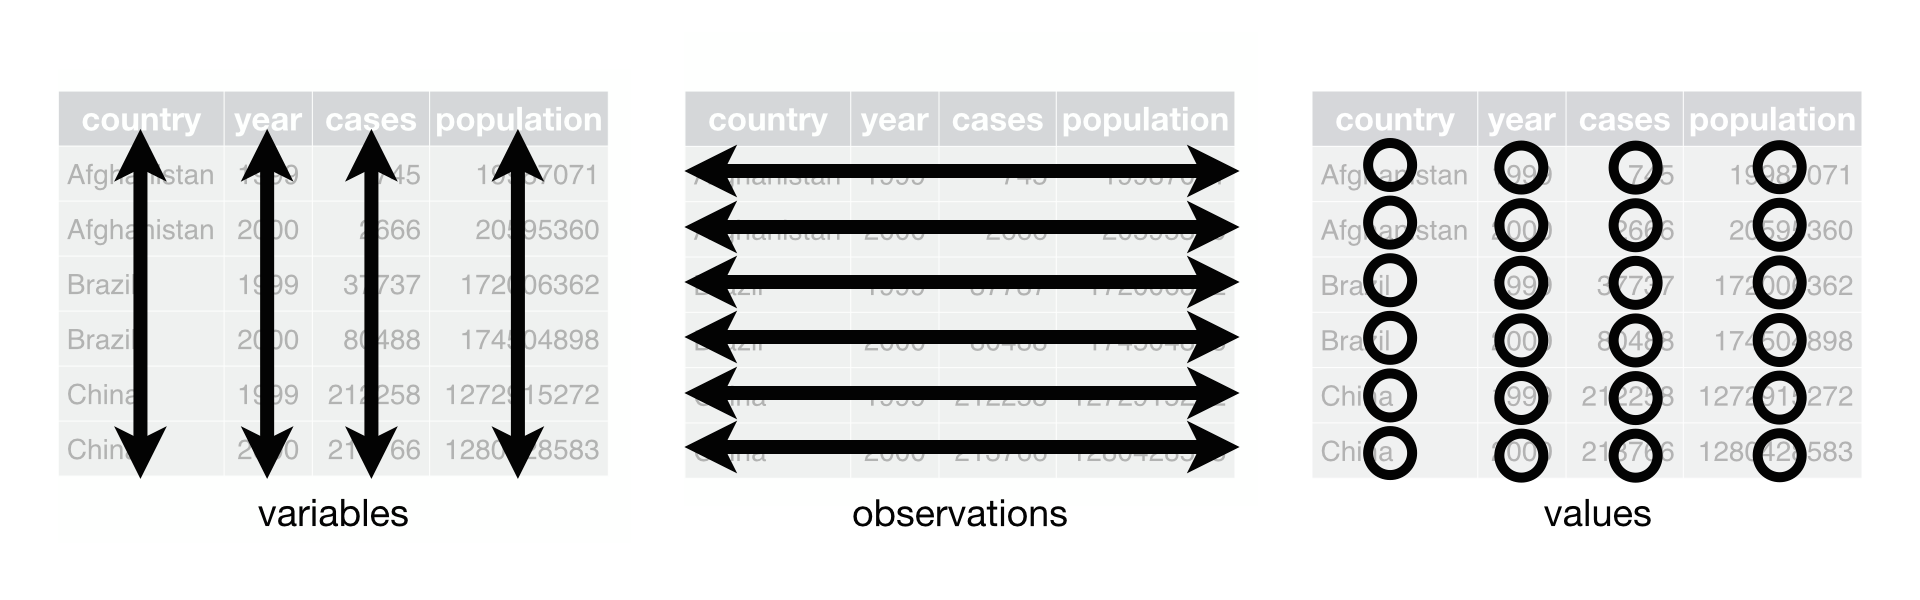
\includegraphics[width=7.11in,height=\textheight]{images/tidy-1.png}

}

\caption{\label{fig-tidy-structure}The following three rules make a
dataset tidy: variables are columns, observations are rows, and values
are cells.}

\end{figure}%

为什么要确保你的数据是整齐的?有 两个主要优势:

\begin{enumerate}
\def\labelenumi{\arabic{enumi}.}
\tightlist
\item
  选择一种一致的数据存储方式具有普遍优势。如果你的数据结构是一致的,学习与之配合使用的工具就更容易,因为它们具有底层的一致性。
\item
  将变量放在列中具有特定的优势,因为这可以让R的矢量化特性大放异彩。正如你在@sec-mutate
  和@sec-summarize
  所学到的,大多数内置的R函数都使用值的向量。这使得处理整齐数据感觉特别自然。
\end{enumerate}

dplyr、ggplot2以及tidyverse中的所有其他包都是为处理整齐数据而设计的。下
面代码是一些展示如何使用\texttt{table1}的小示例。

\begin{Shaded}
\begin{Highlighting}[]
\CommentTok{\# Compute rate per 10,000}
\NormalTok{table1 }\SpecialCharTok{|\textgreater{}}
  \FunctionTok{mutate}\NormalTok{(}\AttributeTok{rate =}\NormalTok{ cases }\SpecialCharTok{/}\NormalTok{ population }\SpecialCharTok{*} \DecValTok{10000}\NormalTok{)}
\CommentTok{\#\textgreater{} \# A tibble: 6 x 5}
\CommentTok{\#\textgreater{}   country      year  cases population  rate}
\CommentTok{\#\textgreater{}   \textless{}chr\textgreater{}       \textless{}dbl\textgreater{}  \textless{}dbl\textgreater{}      \textless{}dbl\textgreater{} \textless{}dbl\textgreater{}}
\CommentTok{\#\textgreater{} 1 Afghanistan  1999    745   19987071 0.373}
\CommentTok{\#\textgreater{} 2 Afghanistan  2000   2666   20595360 1.29 }
\CommentTok{\#\textgreater{} 3 Brazil       1999  37737  172006362 2.19 }
\CommentTok{\#\textgreater{} 4 Brazil       2000  80488  174504898 4.61 }
\CommentTok{\#\textgreater{} 5 China        1999 212258 1272915272 1.67 }
\CommentTok{\#\textgreater{} 6 China        2000 213766 1280428583 1.67}

\CommentTok{\# Compute total cases per year}
\NormalTok{table1 }\SpecialCharTok{|\textgreater{}} 
  \FunctionTok{group\_by}\NormalTok{(year) }\SpecialCharTok{|\textgreater{}} 
  \FunctionTok{summarize}\NormalTok{(}\AttributeTok{total\_cases =} \FunctionTok{sum}\NormalTok{(cases))}
\CommentTok{\#\textgreater{} \# A tibble: 2 x 2}
\CommentTok{\#\textgreater{}    year total\_cases}
\CommentTok{\#\textgreater{}   \textless{}dbl\textgreater{}       \textless{}dbl\textgreater{}}
\CommentTok{\#\textgreater{} 1  1999      250740}
\CommentTok{\#\textgreater{} 2  2000      296920}

\CommentTok{\# Visualize changes over time}
\FunctionTok{ggplot}\NormalTok{(table1, }\FunctionTok{aes}\NormalTok{(}\AttributeTok{x =}\NormalTok{ year, }\AttributeTok{y =}\NormalTok{ cases)) }\SpecialCharTok{+}
  \FunctionTok{geom\_line}\NormalTok{(}\FunctionTok{aes}\NormalTok{(}\AttributeTok{group =}\NormalTok{ country), }\AttributeTok{color =} \StringTok{"grey50"}\NormalTok{) }\SpecialCharTok{+}
  \FunctionTok{geom\_point}\NormalTok{(}\FunctionTok{aes}\NormalTok{(}\AttributeTok{color =}\NormalTok{ country, }\AttributeTok{shape =}\NormalTok{ country)) }\SpecialCharTok{+}
  \FunctionTok{scale\_x\_continuous}\NormalTok{(}\AttributeTok{breaks =} \FunctionTok{c}\NormalTok{(}\DecValTok{1999}\NormalTok{, }\DecValTok{2000}\NormalTok{)) }\CommentTok{\# x{-}axis breaks at 1999 and 2000}
\end{Highlighting}
\end{Shaded}

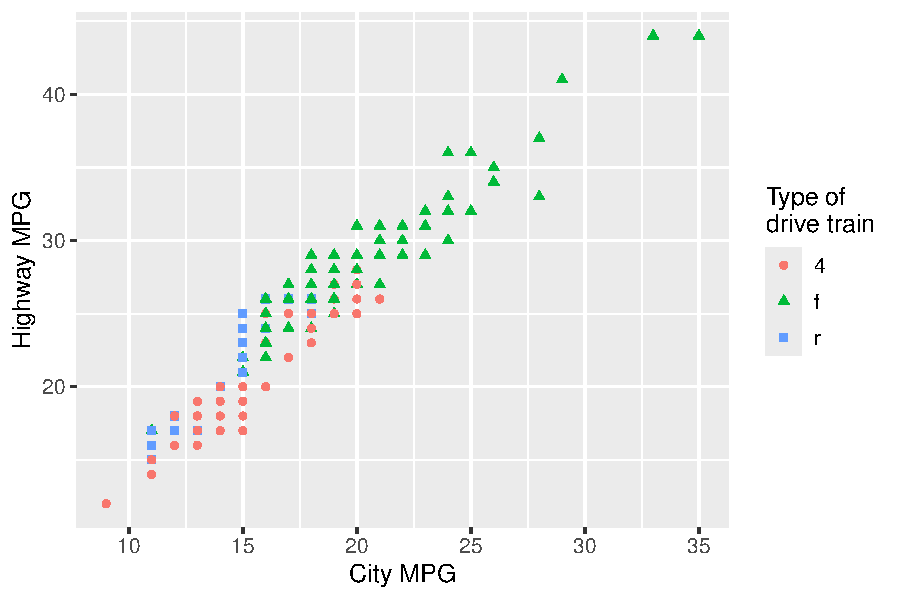
\includegraphics[width=15.625in,height=\textheight]{data-tidy_files/figure-pdf/unnamed-chunk-5-1.pdf}

\subsection{练习}\label{ux7ec3ux4e60-9}

\begin{enumerate}
\def\labelenumi{\arabic{enumi}.}
\item
  对于每个示例表格,描述每个观测值和每列分别代表什么。
\item
  概述你将如何计算\texttt{table2}和\texttt{table3}中的\texttt{rate}。你
  需要执行四个操作:

  \begin{enumerate}
  \def\labelenumii{\alph{enumii}.}
  \tightlist
  \item
    提取每个国家每年的TB病例数;
  \item
    提取每个国家每年对应的人口数;
  \item
    将病例数除以人口数,然后乘以10000;
  \item
    将结果存储回适当的地方.
  \end{enumerate}

  你还没有学习所有实际执行这些操作所需的函数,但应该仍然能够思考出所需的转换步骤。
\end{enumerate}

\section{数据转换---长格式}\label{sec-pivoting}

整齐数据的原则可能看起来如此显而易见,以至于你怀疑是否会遇到不整齐的数据集。然
而,不幸的是,大多数真实数据都是不整齐的。这 主要有两个原因:

\begin{enumerate}
\def\labelenumi{\arabic{enumi}.}
\item
  数据通常是为了方便除了分析以外的其他目的而组织的。例
  如,数据通常以易于数据录入而不是分析的结构来组织。
\item
  大多数人并不熟悉整齐数据的原则,除非你花很多时间处理数据,否则很难自己推导出这些原则。
\end{enumerate}

这意味着大多数实际分析至少需要进行一些整理。首
先要弄清楚基础变量和观测值是什么,有时这很简单,有时你需要咨询最初生成数据的人;接下来,你需要将数据重塑(\textbf{pivot})为整齐的形式,将变量放在列中,将观测值放在行中。

tidyr包提供了两个用于数据重塑的函数:\texttt{pivot\_longer()}和\texttt{pivot\_wider()}。我
们将首先从\texttt{pivot\_longer()}开始,因为它是最常见的情况。让
我们深入探讨一些示例。

\subsection{列名中的数据}\label{sec-billboard}

\texttt{billboard}数据集记录了 2000 年歌曲的 Billboard 排行榜排名:

\begin{Shaded}
\begin{Highlighting}[]
\NormalTok{billboard}
\CommentTok{\#\textgreater{} \# A tibble: 317 x 79}
\CommentTok{\#\textgreater{}   artist       track               date.entered   wk1   wk2   wk3   wk4   wk5}
\CommentTok{\#\textgreater{}   \textless{}chr\textgreater{}        \textless{}chr\textgreater{}               \textless{}date\textgreater{}       \textless{}dbl\textgreater{} \textless{}dbl\textgreater{} \textless{}dbl\textgreater{} \textless{}dbl\textgreater{} \textless{}dbl\textgreater{}}
\CommentTok{\#\textgreater{} 1 2 Pac        Baby Don\textquotesingle{}t Cry (Ke\textasciitilde{} 2000{-}02{-}26      87    82    72    77    87}
\CommentTok{\#\textgreater{} 2 2Ge+her      The Hardest Part O\textasciitilde{} 2000{-}09{-}02      91    87    92    NA    NA}
\CommentTok{\#\textgreater{} 3 3 Doors Down Kryptonite          2000{-}04{-}08      81    70    68    67    66}
\CommentTok{\#\textgreater{} 4 3 Doors Down Loser               2000{-}10{-}21      76    76    72    69    67}
\CommentTok{\#\textgreater{} 5 504 Boyz     Wobble Wobble       2000{-}04{-}15      57    34    25    17    17}
\CommentTok{\#\textgreater{} 6 98\^{}0         Give Me Just One N\textasciitilde{} 2000{-}08{-}19      51    39    34    26    26}
\CommentTok{\#\textgreater{} \# i 311 more rows}
\CommentTok{\#\textgreater{} \# i 71 more variables: wk6 \textless{}dbl\textgreater{}, wk7 \textless{}dbl\textgreater{}, wk8 \textless{}dbl\textgreater{}, wk9 \textless{}dbl\textgreater{}, ...}
\end{Highlighting}
\end{Shaded}

在这个数据集中,每个观测都是一首歌。前
三列(\texttt{artist}、\texttt{track} 和
\texttt{date.entered})是描述歌曲的变量。然
后有76列(\texttt{wk1}-\texttt{wk76})描述了歌曲在每周的排名\footnote{只要这首歌在2000年的某个时间点进入排行榜前100名,它就会被收录,并在它出现后的72周内被追踪。}。
在这里,列名是一个变量(\texttt{week}),而单元格的值是另一个变量(\texttt{rank})。

为了整理这个数据,我们使用 \texttt{pivot\_longer()}:

\begin{Shaded}
\begin{Highlighting}[]
\NormalTok{billboard }\SpecialCharTok{|\textgreater{}} 
  \FunctionTok{pivot\_longer}\NormalTok{(}
    \AttributeTok{cols =} \FunctionTok{starts\_with}\NormalTok{(}\StringTok{"wk"}\NormalTok{), }
    \AttributeTok{names\_to =} \StringTok{"week"}\NormalTok{, }
    \AttributeTok{values\_to =} \StringTok{"rank"}
\NormalTok{  )}
\CommentTok{\#\textgreater{} \# A tibble: 24,092 x 5}
\CommentTok{\#\textgreater{}    artist track                   date.entered week   rank}
\CommentTok{\#\textgreater{}    \textless{}chr\textgreater{}  \textless{}chr\textgreater{}                   \textless{}date\textgreater{}       \textless{}chr\textgreater{} \textless{}dbl\textgreater{}}
\CommentTok{\#\textgreater{}  1 2 Pac  Baby Don\textquotesingle{}t Cry (Keep... 2000{-}02{-}26   wk1      87}
\CommentTok{\#\textgreater{}  2 2 Pac  Baby Don\textquotesingle{}t Cry (Keep... 2000{-}02{-}26   wk2      82}
\CommentTok{\#\textgreater{}  3 2 Pac  Baby Don\textquotesingle{}t Cry (Keep... 2000{-}02{-}26   wk3      72}
\CommentTok{\#\textgreater{}  4 2 Pac  Baby Don\textquotesingle{}t Cry (Keep... 2000{-}02{-}26   wk4      77}
\CommentTok{\#\textgreater{}  5 2 Pac  Baby Don\textquotesingle{}t Cry (Keep... 2000{-}02{-}26   wk5      87}
\CommentTok{\#\textgreater{}  6 2 Pac  Baby Don\textquotesingle{}t Cry (Keep... 2000{-}02{-}26   wk6      94}
\CommentTok{\#\textgreater{}  7 2 Pac  Baby Don\textquotesingle{}t Cry (Keep... 2000{-}02{-}26   wk7      99}
\CommentTok{\#\textgreater{}  8 2 Pac  Baby Don\textquotesingle{}t Cry (Keep... 2000{-}02{-}26   wk8      NA}
\CommentTok{\#\textgreater{}  9 2 Pac  Baby Don\textquotesingle{}t Cry (Keep... 2000{-}02{-}26   wk9      NA}
\CommentTok{\#\textgreater{} 10 2 Pac  Baby Don\textquotesingle{}t Cry (Keep... 2000{-}02{-}26   wk10     NA}
\CommentTok{\#\textgreater{} \# i 24,082 more rows}
\end{Highlighting}
\end{Shaded}

数据之后,有三个关键参数:

\begin{itemize}
\tightlist
\item
  \texttt{cols}
  指定了哪些列需要进行重塑,即哪些列不是变量。这个参数使用了与\texttt{select()}相同的语法,因此在这里我们可以使用\texttt{!c(artist,\ track,\ date.entered)}或者\texttt{starts\_with("wk")}。
\item
  \texttt{names\_to}
  用于命名列名中存储的变量,我们将其命名为\texttt{week}
\item
  \texttt{values\_to}
  用于命名单元格值中存储的变量,我们将其命名为\texttt{rank}。
\end{itemize}

请注意,代码中\texttt{“week”}和\texttt{“rank”}被引号括起来,因为这些是我们创建的新变量,在运行\texttt{pivot\_longer()}调用时它们还不在数据中。

现在让我们把注意力转向得到的长数据框。如
果一首歌在前100名中的时间少于76周,会发生什么?以 2 Pac的《Baby Don't
Cry》为例。上
面的输出表明它只在前100名中待了7周,而其余所有周都填充了缺失值。这
些NA并不真正代表未知的观测值,它们是由于数据集的结构而被迫存在的,因此我们可以要求\texttt{pivot\_longer()}通过设置\texttt{values\_drop\_na\ =\ TRUE}来删除它们:

\begin{Shaded}
\begin{Highlighting}[]
\NormalTok{billboard }\SpecialCharTok{|\textgreater{}} 
  \FunctionTok{pivot\_longer}\NormalTok{(}
    \AttributeTok{cols =} \FunctionTok{starts\_with}\NormalTok{(}\StringTok{"wk"}\NormalTok{), }
    \AttributeTok{names\_to =} \StringTok{"week"}\NormalTok{, }
    \AttributeTok{values\_to =} \StringTok{"rank"}\NormalTok{,}
    \AttributeTok{values\_drop\_na =} \ConstantTok{TRUE}
\NormalTok{  )}
\CommentTok{\#\textgreater{} \# A tibble: 5,307 x 5}
\CommentTok{\#\textgreater{}   artist track                   date.entered week   rank}
\CommentTok{\#\textgreater{}   \textless{}chr\textgreater{}  \textless{}chr\textgreater{}                   \textless{}date\textgreater{}       \textless{}chr\textgreater{} \textless{}dbl\textgreater{}}
\CommentTok{\#\textgreater{} 1 2 Pac  Baby Don\textquotesingle{}t Cry (Keep... 2000{-}02{-}26   wk1      87}
\CommentTok{\#\textgreater{} 2 2 Pac  Baby Don\textquotesingle{}t Cry (Keep... 2000{-}02{-}26   wk2      82}
\CommentTok{\#\textgreater{} 3 2 Pac  Baby Don\textquotesingle{}t Cry (Keep... 2000{-}02{-}26   wk3      72}
\CommentTok{\#\textgreater{} 4 2 Pac  Baby Don\textquotesingle{}t Cry (Keep... 2000{-}02{-}26   wk4      77}
\CommentTok{\#\textgreater{} 5 2 Pac  Baby Don\textquotesingle{}t Cry (Keep... 2000{-}02{-}26   wk5      87}
\CommentTok{\#\textgreater{} 6 2 Pac  Baby Don\textquotesingle{}t Cry (Keep... 2000{-}02{-}26   wk6      94}
\CommentTok{\#\textgreater{} \# i 5,301 more rows}
\end{Highlighting}
\end{Shaded}

现在行数大大减少,这表明许多包含\texttt{NA}的行已被删除。

你也可能会好奇,如果一首歌在前100名中超过76周,会发生什么?从
这些数据中我们无法得知,但你可以猜测数据集会添加额外的列,如\texttt{wk77}、\texttt{wk78}等。

现在数据已经整齐了,但我们可以通过使用\texttt{mutate()}和\texttt{readr::parse\_number()}将\texttt{week}的值从字符串转换为数字,以使未来的计算更加方便。\texttt{p}
\texttt{arse\_number()}是一个方便的函数,它会从字符串中提取第一个数字,忽略其他所有文本。

\begin{Shaded}
\begin{Highlighting}[]
\NormalTok{billboard\_longer }\OtherTok{\textless{}{-}}\NormalTok{ billboard }\SpecialCharTok{|\textgreater{}} 
  \FunctionTok{pivot\_longer}\NormalTok{(}
    \AttributeTok{cols =} \FunctionTok{starts\_with}\NormalTok{(}\StringTok{"wk"}\NormalTok{), }
    \AttributeTok{names\_to =} \StringTok{"week"}\NormalTok{, }
    \AttributeTok{values\_to =} \StringTok{"rank"}\NormalTok{,}
    \AttributeTok{values\_drop\_na =} \ConstantTok{TRUE}
\NormalTok{  ) }\SpecialCharTok{|\textgreater{}} 
  \FunctionTok{mutate}\NormalTok{(}
    \AttributeTok{week =} \FunctionTok{parse\_number}\NormalTok{(week)}
\NormalTok{  )}
\NormalTok{billboard\_longer}
\CommentTok{\#\textgreater{} \# A tibble: 5,307 x 5}
\CommentTok{\#\textgreater{}   artist track                   date.entered  week  rank}
\CommentTok{\#\textgreater{}   \textless{}chr\textgreater{}  \textless{}chr\textgreater{}                   \textless{}date\textgreater{}       \textless{}dbl\textgreater{} \textless{}dbl\textgreater{}}
\CommentTok{\#\textgreater{} 1 2 Pac  Baby Don\textquotesingle{}t Cry (Keep... 2000{-}02{-}26       1    87}
\CommentTok{\#\textgreater{} 2 2 Pac  Baby Don\textquotesingle{}t Cry (Keep... 2000{-}02{-}26       2    82}
\CommentTok{\#\textgreater{} 3 2 Pac  Baby Don\textquotesingle{}t Cry (Keep... 2000{-}02{-}26       3    72}
\CommentTok{\#\textgreater{} 4 2 Pac  Baby Don\textquotesingle{}t Cry (Keep... 2000{-}02{-}26       4    77}
\CommentTok{\#\textgreater{} 5 2 Pac  Baby Don\textquotesingle{}t Cry (Keep... 2000{-}02{-}26       5    87}
\CommentTok{\#\textgreater{} 6 2 Pac  Baby Don\textquotesingle{}t Cry (Keep... 2000{-}02{-}26       6    94}
\CommentTok{\#\textgreater{} \# i 5,301 more rows}
\end{Highlighting}
\end{Shaded}

既然我们已经将所有周数放入一个变量,并将所有排名值放入另一个变量,现在可以很好地可视化歌曲排名如何随时间变化。下
面的代码展示了这一点,结果位于@fig-billboard-ranks 。我
们可以看到,很少有歌曲能在前100名中保持超过20周的时间。

\begin{Shaded}
\begin{Highlighting}[]
\NormalTok{billboard\_longer }\SpecialCharTok{|\textgreater{}} 
  \FunctionTok{ggplot}\NormalTok{(}\FunctionTok{aes}\NormalTok{(}\AttributeTok{x =}\NormalTok{ week, }\AttributeTok{y =}\NormalTok{ rank, }\AttributeTok{group =}\NormalTok{ track)) }\SpecialCharTok{+} 
  \FunctionTok{geom\_line}\NormalTok{(}\AttributeTok{alpha =} \FloatTok{0.25}\NormalTok{) }\SpecialCharTok{+} 
  \FunctionTok{scale\_y\_reverse}\NormalTok{()}
\end{Highlighting}
\end{Shaded}

\begin{figure}[H]

\centering{

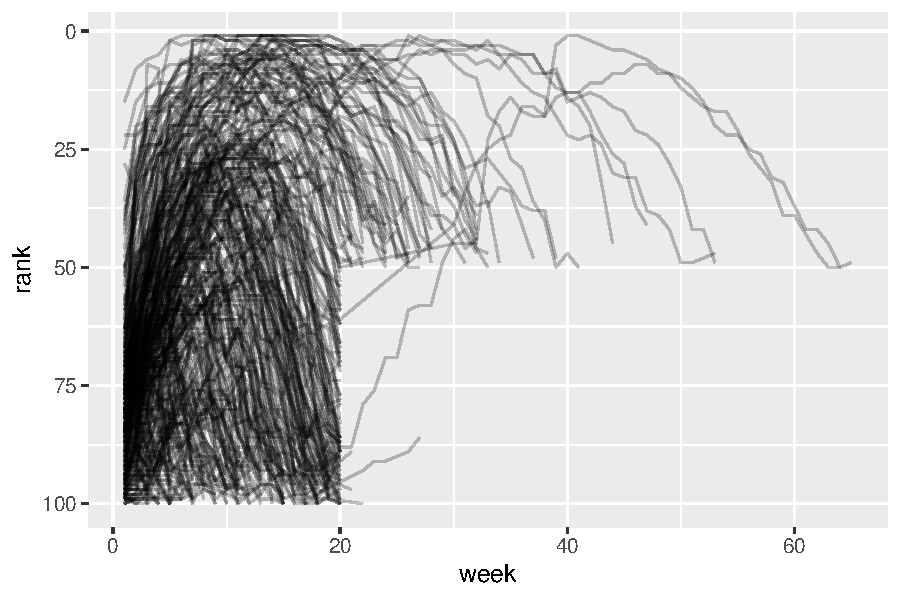
\includegraphics[width=18.75in,height=\textheight]{data-tidy_files/figure-pdf/fig-billboard-ranks-1.pdf}

}

\caption{\label{fig-billboard-ranks}A line plot showing how the rank of
a song changes over time.}

\end{figure}%

\subsection{pivoting是如何工作的?}\label{pivotingux662fux5982ux4f55ux5de5ux4f5cux7684}

既然你已经看到了我们如何使用pivoting来重塑我们的数据,让我们花点时间来直观地理解pivoting对数据做了什么。让
我们从一个非常简单的数据集开始,以便更容易地看到发生了什么。假
设我们有三个患者,\texttt{id}分别为A、B和C,对每个患者进行了两次血压测量。我
们使用\texttt{tribble()}来创建这些数据,tribble()是一个易用的函数,这里通过手动构造小型tibble对象:

\begin{Shaded}
\begin{Highlighting}[]
\NormalTok{df }\OtherTok{\textless{}{-}} \FunctionTok{tribble}\NormalTok{(}
  \SpecialCharTok{\textasciitilde{}}\NormalTok{id,  }\SpecialCharTok{\textasciitilde{}}\NormalTok{bp1, }\SpecialCharTok{\textasciitilde{}}\NormalTok{bp2,}
   \StringTok{"A"}\NormalTok{,  }\DecValTok{100}\NormalTok{,  }\DecValTok{120}\NormalTok{,}
   \StringTok{"B"}\NormalTok{,  }\DecValTok{140}\NormalTok{,  }\DecValTok{115}\NormalTok{,}
   \StringTok{"C"}\NormalTok{,  }\DecValTok{120}\NormalTok{,  }\DecValTok{125}
\NormalTok{)}
\end{Highlighting}
\end{Shaded}

我们希望新数据集有三个变量:id(已存在)、measurement(列名)和value(单元格值)。为
了实现这一点,我们需要将df重塑(pivot)为更长的格式:

\begin{Shaded}
\begin{Highlighting}[]
\NormalTok{df }\SpecialCharTok{|\textgreater{}} 
  \FunctionTok{pivot\_longer}\NormalTok{(}
    \AttributeTok{cols =}\NormalTok{ bp1}\SpecialCharTok{:}\NormalTok{bp2,}
    \AttributeTok{names\_to =} \StringTok{"measurement"}\NormalTok{,}
    \AttributeTok{values\_to =} \StringTok{"value"}
\NormalTok{  )}
\CommentTok{\#\textgreater{} \# A tibble: 6 x 3}
\CommentTok{\#\textgreater{}   id    measurement value}
\CommentTok{\#\textgreater{}   \textless{}chr\textgreater{} \textless{}chr\textgreater{}       \textless{}dbl\textgreater{}}
\CommentTok{\#\textgreater{} 1 A     bp1           100}
\CommentTok{\#\textgreater{} 2 A     bp2           120}
\CommentTok{\#\textgreater{} 3 B     bp1           140}
\CommentTok{\#\textgreater{} 4 B     bp2           115}
\CommentTok{\#\textgreater{} 5 C     bp1           120}
\CommentTok{\#\textgreater{} 6 C     bp2           125}
\end{Highlighting}
\end{Shaded}

重塑是如何工作的?如 果我们按列思考,就会更容易理解。如
图~\ref{fig-pivot-variables}
所示,在原始数据集中已经是变量的列(如id)的值需要被重复,每个被重塑的列重复一次。

\begin{figure}

\centering{

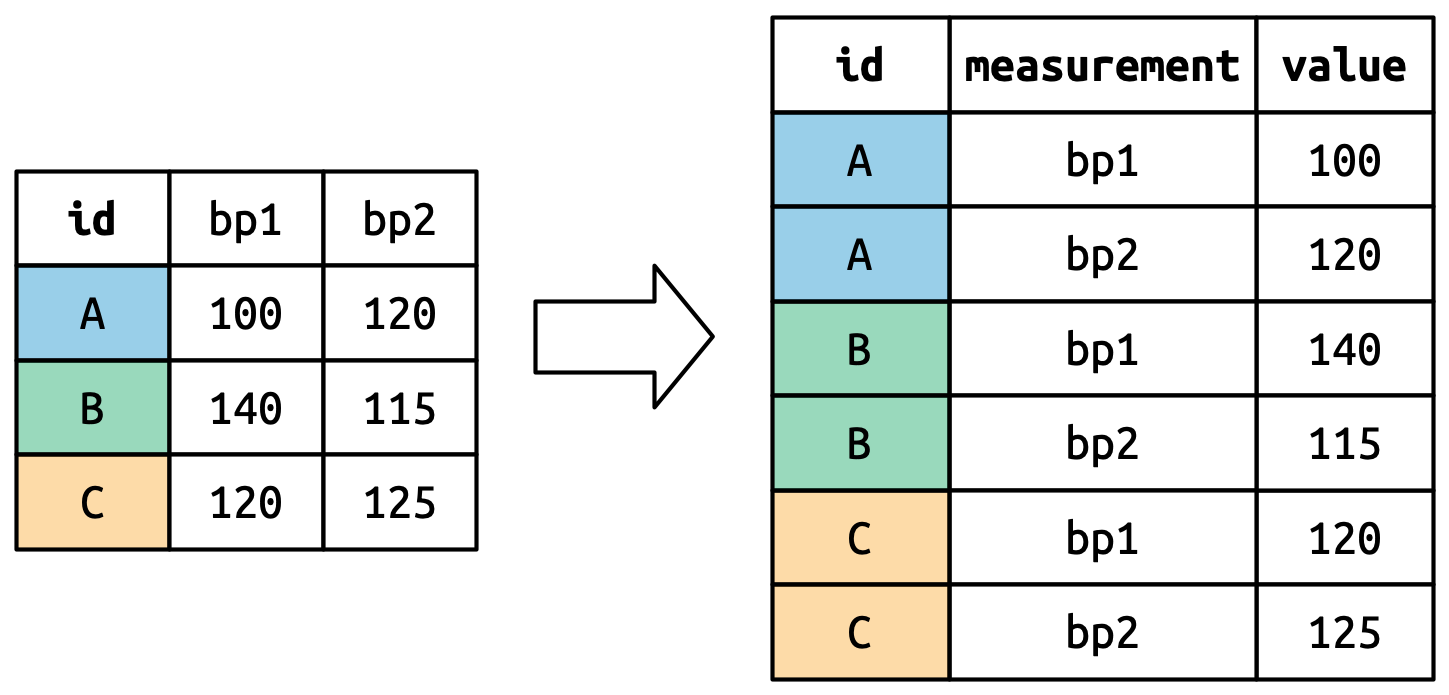
\includegraphics[width=5.37in,height=\textheight]{diagrams/tidy-data/variables.png}

}

\caption{\label{fig-pivot-variables}Columns that are already variables
need to be repeated, once for each column that is pivoted.}

\end{figure}%

列名变成新变量的值,新变量的名称由\texttt{names\_to}定义,如@fig-pivot-names
所示。它 们需要在原始数据集的每一行中重复一次。

\begin{figure}

\centering{

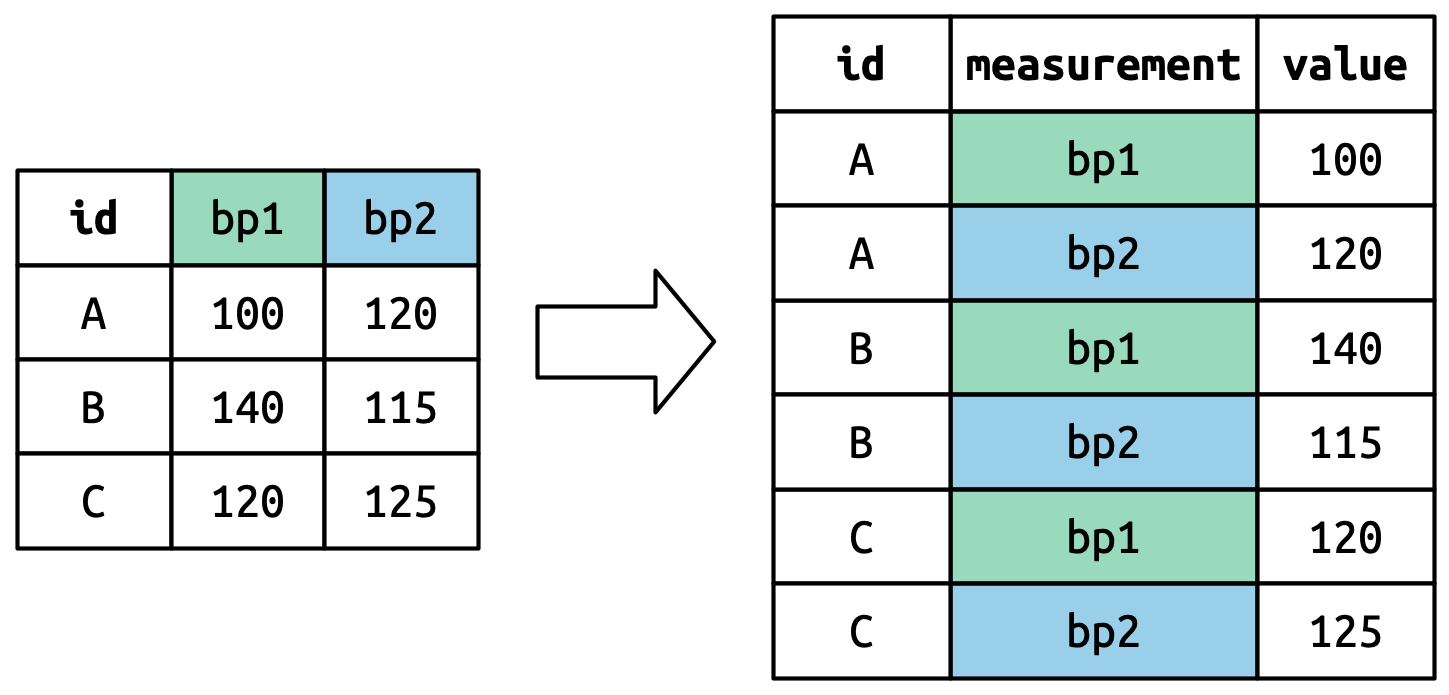
\includegraphics[width=5.37in,height=\textheight]{diagrams/tidy-data/column-names.png}

}

\caption{\label{fig-pivot-names}The column names of pivoted columns
become values in a new column. The values need to be repeated once for
each row of the original dataset.}

\end{figure}%

单元格值也变成新变量的值,新变量的名称由\texttt{values\_to}定义。它
们被逐行地展开。@ fig-pivot-values 展示了这一过程。

\begin{figure}

\centering{

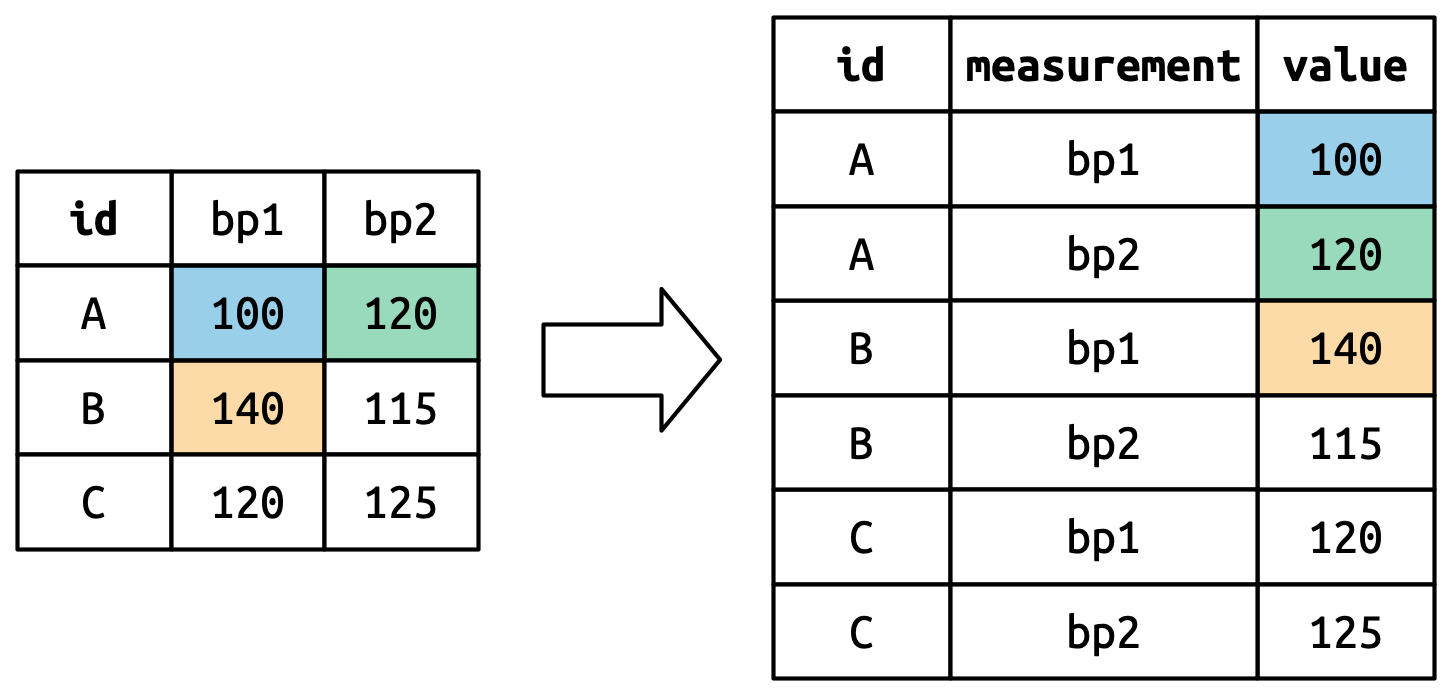
\includegraphics[width=5.37in,height=\textheight]{diagrams/tidy-data/cell-values.png}

}

\caption{\label{fig-pivot-values}The number of values is preserved (not
repeated), but unwound row-by-row.}

\end{figure}%

\subsection{列名中包含多个变量}\label{ux5217ux540dux4e2dux5305ux542bux591aux4e2aux53d8ux91cf}

当列名中融合了多个信息片段而你希望将这些信息分散到独立的新变量中时,情况就会变得更加复杂。这
里以你之前看到的\texttt{table1}等表的源头数据集\texttt{who2}为例:

\begin{Shaded}
\begin{Highlighting}[]
\NormalTok{who2}
\CommentTok{\#\textgreater{} \# A tibble: 7,240 x 58}
\CommentTok{\#\textgreater{}   country      year sp\_m\_014 sp\_m\_1524 sp\_m\_2534 sp\_m\_3544 sp\_m\_4554}
\CommentTok{\#\textgreater{}   \textless{}chr\textgreater{}       \textless{}dbl\textgreater{}    \textless{}dbl\textgreater{}     \textless{}dbl\textgreater{}     \textless{}dbl\textgreater{}     \textless{}dbl\textgreater{}     \textless{}dbl\textgreater{}}
\CommentTok{\#\textgreater{} 1 Afghanistan  1980       NA        NA        NA        NA        NA}
\CommentTok{\#\textgreater{} 2 Afghanistan  1981       NA        NA        NA        NA        NA}
\CommentTok{\#\textgreater{} 3 Afghanistan  1982       NA        NA        NA        NA        NA}
\CommentTok{\#\textgreater{} 4 Afghanistan  1983       NA        NA        NA        NA        NA}
\CommentTok{\#\textgreater{} 5 Afghanistan  1984       NA        NA        NA        NA        NA}
\CommentTok{\#\textgreater{} 6 Afghanistan  1985       NA        NA        NA        NA        NA}
\CommentTok{\#\textgreater{} \# i 7,234 more rows}
\CommentTok{\#\textgreater{} \# i 51 more variables: sp\_m\_5564 \textless{}dbl\textgreater{}, sp\_m\_65 \textless{}dbl\textgreater{}, sp\_f\_014 \textless{}dbl\textgreater{}, ...}
\end{Highlighting}
\end{Shaded}

这个数据集由世界卫生组织收集,记录了关于结核病诊断的信息,其中有两个列已经是变量且易于解读:\texttt{country}和\texttt{year}。接
着是56个像\texttt{sp\_m\_014}、\texttt{ep\_m\_4554}和\texttt{rel\_m\_3544}这样的列。如
果你长时间盯着这些列看就会发现一个规律。每
个列名都由三部分组成,由\texttt{\_}分隔。第
一部分\texttt{sp}/\texttt{rel}/\texttt{ep}描述了用于诊断的方法;第二部分\texttt{m}/\texttt{f}是性别(在这个数据集中被编码为二进制变量);第三部分,\texttt{014}/\texttt{1524}/\texttt{2534}/\texttt{3544}/\texttt{4554}/\texttt{5564}/\texttt{65}是年龄范围(例如,\texttt{014}代表0-14岁)。

因此,在这种情况下,\texttt{who2}数据集中记录了六条信息:country和year(已经是列);诊断方法、性别和年龄范围类别(包含在其他列名中),以及该类别中的患者数量(单元格值)。为
了将这六条信息组织到六个单独的列中,我们使用\texttt{pivot\_longer()}函数,并为\texttt{names\_to}提供一个列名字符串向量,以及为\texttt{names\_sep}提供一个指令来将原始变量名分割成片段,并为\texttt{values\_to}提供一个列名:

\begin{Shaded}
\begin{Highlighting}[]
\NormalTok{who2 }\SpecialCharTok{|\textgreater{}} 
  \FunctionTok{pivot\_longer}\NormalTok{(}
    \AttributeTok{cols =} \SpecialCharTok{!}\NormalTok{(country}\SpecialCharTok{:}\NormalTok{year),}
    \AttributeTok{names\_to =} \FunctionTok{c}\NormalTok{(}\StringTok{"diagnosis"}\NormalTok{, }\StringTok{"gender"}\NormalTok{, }\StringTok{"age"}\NormalTok{), }
    \AttributeTok{names\_sep =} \StringTok{"\_"}\NormalTok{,}
    \AttributeTok{values\_to =} \StringTok{"count"}
\NormalTok{  )}
\CommentTok{\#\textgreater{} \# A tibble: 405,440 x 6}
\CommentTok{\#\textgreater{}   country      year diagnosis gender age   count}
\CommentTok{\#\textgreater{}   \textless{}chr\textgreater{}       \textless{}dbl\textgreater{} \textless{}chr\textgreater{}     \textless{}chr\textgreater{}  \textless{}chr\textgreater{} \textless{}dbl\textgreater{}}
\CommentTok{\#\textgreater{} 1 Afghanistan  1980 sp        m      014      NA}
\CommentTok{\#\textgreater{} 2 Afghanistan  1980 sp        m      1524     NA}
\CommentTok{\#\textgreater{} 3 Afghanistan  1980 sp        m      2534     NA}
\CommentTok{\#\textgreater{} 4 Afghanistan  1980 sp        m      3544     NA}
\CommentTok{\#\textgreater{} 5 Afghanistan  1980 sp        m      4554     NA}
\CommentTok{\#\textgreater{} 6 Afghanistan  1980 sp        m      5564     NA}
\CommentTok{\#\textgreater{} \# i 405,434 more rows}
\end{Highlighting}
\end{Shaded}

除了\texttt{names\_sep}之外,你还可以使用\texttt{names\_pattern}。当
你在@sec-regular-expressions
学习了正则表达式之后,就可以使用它来从更复杂的命名场景中提取变量。

从概念上讲,这只是在你之前看到的简单情况上做了微小的变化。@
sec-regular-expressions
展示了基本思想:现在,列名不再只是转换为一个单独的列,而是转换为多个列。你
可以想象这个过程分为两步(首先转换然后分割),但实际上它是在一步中完成的,因为这样更快。

\begin{figure}

\centering{

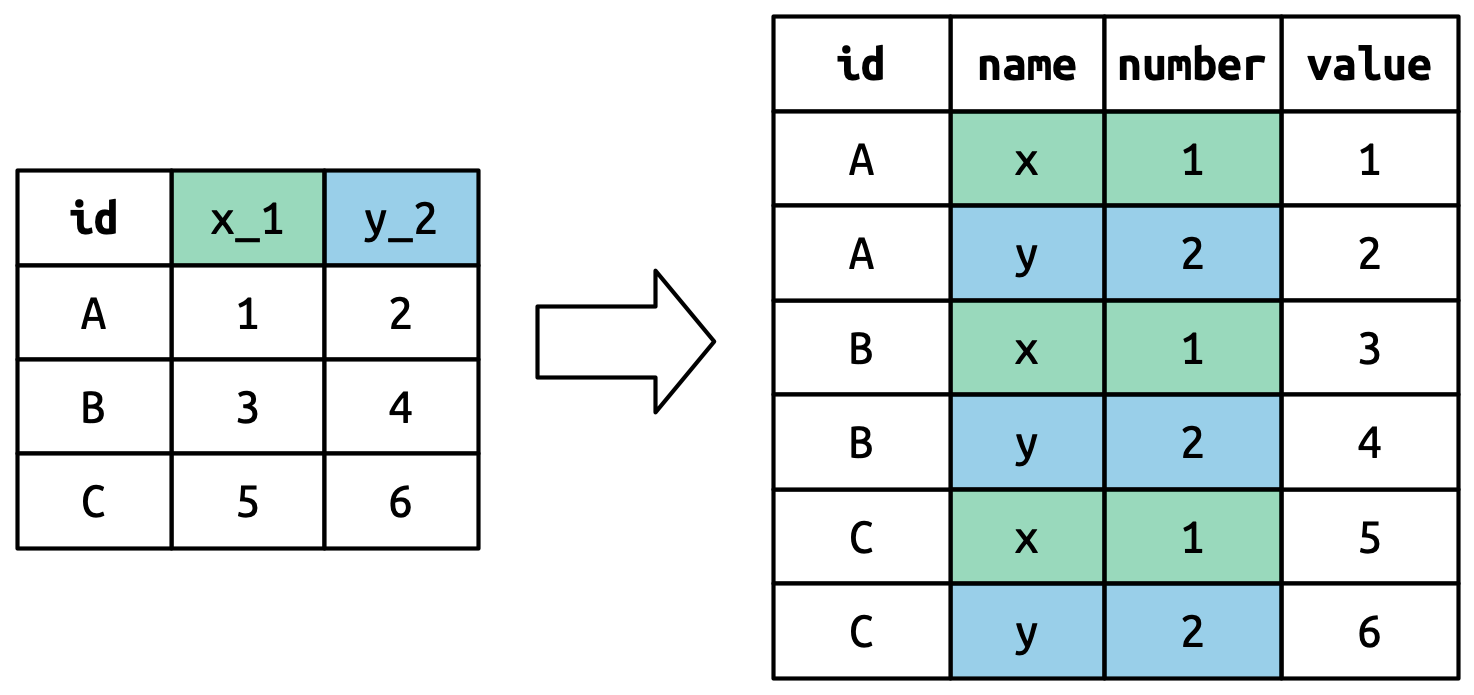
\includegraphics[width=5.46in,height=\textheight]{diagrams/tidy-data/multiple-names.png}

}

\caption{\label{fig-pivot-multiple-names}Pivoting columns with multiple
pieces of information in the names means that each column name now fills
in values in multiple output columns.}

\end{figure}%

\subsection{列标题中的数据和变量名}\label{ux5217ux6807ux9898ux4e2dux7684ux6570ux636eux548cux53d8ux91cfux540d}

接下来更复杂的步骤是当列名包含变量值和变量名的混合时。例
如,以\texttt{household}数据集为例:

\begin{Shaded}
\begin{Highlighting}[]
\NormalTok{household}
\CommentTok{\#\textgreater{} \# A tibble: 5 x 5}
\CommentTok{\#\textgreater{}   family dob\_child1 dob\_child2 name\_child1 name\_child2}
\CommentTok{\#\textgreater{}    \textless{}int\textgreater{} \textless{}date\textgreater{}     \textless{}date\textgreater{}     \textless{}chr\textgreater{}       \textless{}chr\textgreater{}      }
\CommentTok{\#\textgreater{} 1      1 1998{-}11{-}26 2000{-}01{-}29 Susan       Jose       }
\CommentTok{\#\textgreater{} 2      2 1996{-}06{-}22 NA         Mark        \textless{}NA\textgreater{}       }
\CommentTok{\#\textgreater{} 3      3 2002{-}07{-}11 2004{-}04{-}05 Sam         Seth       }
\CommentTok{\#\textgreater{} 4      4 2004{-}10{-}10 2009{-}08{-}27 Craig       Khai       }
\CommentTok{\#\textgreater{} 5      5 2000{-}12{-}05 2005{-}02{-}28 Parker      Gracie}
\end{Highlighting}
\end{Shaded}

这个数据集包含了五个家庭的数据,每个家庭最多有两个孩子的姓名和出生日期。数
据集中的新挑战是列名包含了两个变量的名称(\texttt{dob}、\texttt{name})和另一个变量(\texttt{child},其值为1或2)的值。为
了解决这个问题,我们再次需要向\texttt{names\_to}提供一个向量,但这次我们使用特殊的\texttt{".value"}哨兵值(sentinel);这不是变量的名称,而是一个独特的值,它告诉\texttt{pivot\_longer()}做一些不同的事情。这
会覆盖通常的\texttt{values\_to}参数,使用重塑后的列名的第一个组成部分作为输出中的变量名。

\begin{Shaded}
\begin{Highlighting}[]
\NormalTok{household }\SpecialCharTok{|\textgreater{}} 
  \FunctionTok{pivot\_longer}\NormalTok{(}
    \AttributeTok{cols =} \SpecialCharTok{!}\NormalTok{family, }
    \AttributeTok{names\_to =} \FunctionTok{c}\NormalTok{(}\StringTok{".value"}\NormalTok{, }\StringTok{"child"}\NormalTok{), }
    \AttributeTok{names\_sep =} \StringTok{"\_"}\NormalTok{, }
    \AttributeTok{values\_drop\_na =} \ConstantTok{TRUE}
\NormalTok{  )}
\CommentTok{\#\textgreater{} \# A tibble: 9 x 4}
\CommentTok{\#\textgreater{}   family child  dob        name }
\CommentTok{\#\textgreater{}    \textless{}int\textgreater{} \textless{}chr\textgreater{}  \textless{}date\textgreater{}     \textless{}chr\textgreater{}}
\CommentTok{\#\textgreater{} 1      1 child1 1998{-}11{-}26 Susan}
\CommentTok{\#\textgreater{} 2      1 child2 2000{-}01{-}29 Jose }
\CommentTok{\#\textgreater{} 3      2 child1 1996{-}06{-}22 Mark }
\CommentTok{\#\textgreater{} 4      3 child1 2002{-}07{-}11 Sam  }
\CommentTok{\#\textgreater{} 5      3 child2 2004{-}04{-}05 Seth }
\CommentTok{\#\textgreater{} 6      4 child1 2004{-}10{-}10 Craig}
\CommentTok{\#\textgreater{} \# i 3 more rows}
\end{Highlighting}
\end{Shaded}

由于输入数据的格式,必须创建一些明确的缺失变量(例如,对于只有一个孩子的家庭)通过设置\texttt{values\_drop\_na\ =\ TRUE},我们可以选择忽略这些由于数据不完整而产生的NA值。。

图~\ref{fig-pivot-names-and-values}
通过一个更简单的示例说明了基本思想。当
您在\texttt{names\_to}中使用\texttt{".value"}时,输入中的列名对输出中的值和变量名都有贡献。

\begin{figure}

\centering{

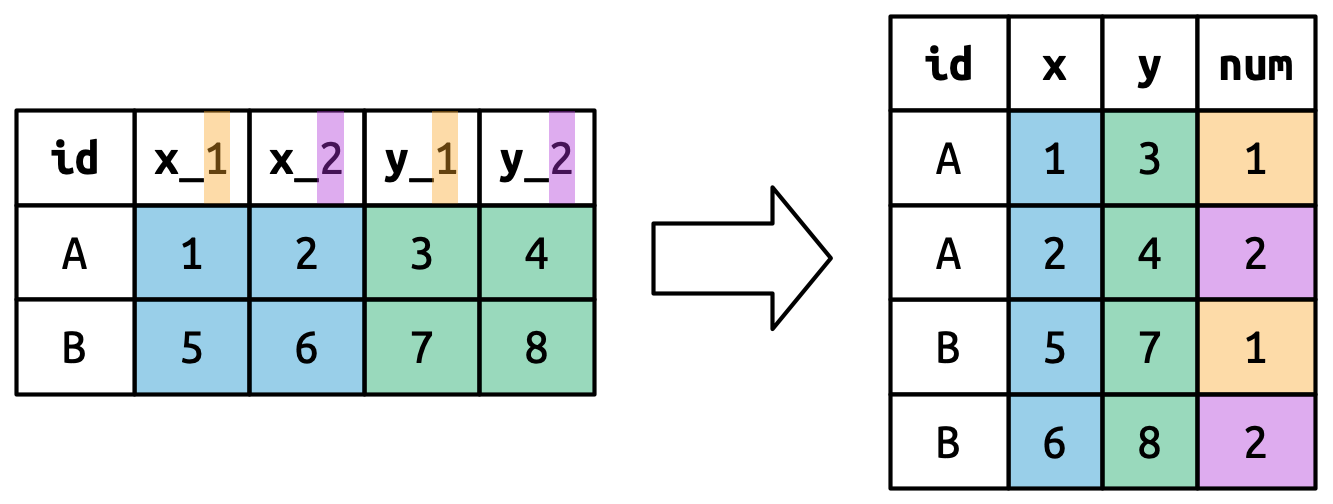
\includegraphics[width=4.94in,height=\textheight]{diagrams/tidy-data/names-and-values.png}

}

\caption{\label{fig-pivot-names-and-values}Pivoting with
\texttt{names\_to\ =\ c(".value",\ "num")} splits the column names into
two components: the first part determines the output column name
(\texttt{x} or \texttt{y}), and the second part determines the value of
the \texttt{num} column.}

\end{figure}%

\section{数据转换---宽格式}\label{ux6570ux636eux8f6cux6362ux5bbdux683cux5f0f}

到目前为止,我们已经使用\texttt{pivot\_longer()}函数来解决了一个常见问题,即值最终出现在列名中的情况。接
下来,我们将转置(HA
HA,这里是一个双关语,因为pivot在英语中也有``转置''的意思)到\texttt{pivot\_wider()}函数,该函数通过增加列和减少行来使数据集变宽,这在一个观测分布在多行时特别有用。这
种情况在实际数据中较少出现,但在处理政府数据时似乎很常见。

我们将首先查看\texttt{cms\_patient\_experience}数据集,这是一个来自医疗保险和医疗补助服务中心(Centers
of Medicare and Medicaid
Services)的数据集,该数据集收集了关于患者体验的数据:

\begin{Shaded}
\begin{Highlighting}[]
\NormalTok{cms\_patient\_experience}
\CommentTok{\#\textgreater{} \# A tibble: 500 x 5}
\CommentTok{\#\textgreater{}   org\_pac\_id org\_nm                     measure\_cd   measure\_title   prf\_rate}
\CommentTok{\#\textgreater{}   \textless{}chr\textgreater{}      \textless{}chr\textgreater{}                      \textless{}chr\textgreater{}        \textless{}chr\textgreater{}              \textless{}dbl\textgreater{}}
\CommentTok{\#\textgreater{} 1 0446157747 USC CARE MEDICAL GROUP INC CAHPS\_GRP\_1  CAHPS for MIPS\textasciitilde{}       63}
\CommentTok{\#\textgreater{} 2 0446157747 USC CARE MEDICAL GROUP INC CAHPS\_GRP\_2  CAHPS for MIPS\textasciitilde{}       87}
\CommentTok{\#\textgreater{} 3 0446157747 USC CARE MEDICAL GROUP INC CAHPS\_GRP\_3  CAHPS for MIPS\textasciitilde{}       86}
\CommentTok{\#\textgreater{} 4 0446157747 USC CARE MEDICAL GROUP INC CAHPS\_GRP\_5  CAHPS for MIPS\textasciitilde{}       57}
\CommentTok{\#\textgreater{} 5 0446157747 USC CARE MEDICAL GROUP INC CAHPS\_GRP\_8  CAHPS for MIPS\textasciitilde{}       85}
\CommentTok{\#\textgreater{} 6 0446157747 USC CARE MEDICAL GROUP INC CAHPS\_GRP\_12 CAHPS for MIPS\textasciitilde{}       24}
\CommentTok{\#\textgreater{} \# i 494 more rows}
\end{Highlighting}
\end{Shaded}

被研究的核心单位是组织,但每个组织都分布在六行中,每行代表调查组织中的一个测量值。我
们可以通过使用\texttt{distinct()}函数来查看\texttt{measure\_cd}和\texttt{measure\_title}值的完整集。

\begin{Shaded}
\begin{Highlighting}[]
\NormalTok{cms\_patient\_experience }\SpecialCharTok{|\textgreater{}} 
  \FunctionTok{distinct}\NormalTok{(measure\_cd, measure\_title)}
\CommentTok{\#\textgreater{} \# A tibble: 6 x 2}
\CommentTok{\#\textgreater{}   measure\_cd   measure\_title                                                 }
\CommentTok{\#\textgreater{}   \textless{}chr\textgreater{}        \textless{}chr\textgreater{}                                                         }
\CommentTok{\#\textgreater{} 1 CAHPS\_GRP\_1  CAHPS for MIPS SSM: Getting Timely Care, Appointments, and In\textasciitilde{}}
\CommentTok{\#\textgreater{} 2 CAHPS\_GRP\_2  CAHPS for MIPS SSM: How Well Providers Communicate            }
\CommentTok{\#\textgreater{} 3 CAHPS\_GRP\_3  CAHPS for MIPS SSM: Patient\textquotesingle{}s Rating of Provider              }
\CommentTok{\#\textgreater{} 4 CAHPS\_GRP\_5  CAHPS for MIPS SSM: Health Promotion and Education            }
\CommentTok{\#\textgreater{} 5 CAHPS\_GRP\_8  CAHPS for MIPS SSM: Courteous and Helpful Office Staff        }
\CommentTok{\#\textgreater{} 6 CAHPS\_GRP\_12 CAHPS for MIPS SSM: Stewardship of Patient Resources}
\end{Highlighting}
\end{Shaded}

这两列都不会成为特别好的变量名:\texttt{measure\_cd}没有暗示变量的含义,而\texttt{measure\_title}是一个包含空格的长句子。目
前我们将使用\texttt{measure\_cd}作为新列名的来源,但在实际分析中,你可能希望创建既简短又有意义的变量名。

\texttt{pivot\_wider()}与\texttt{pivot\_longer()}的操作正好相反。它
不需要定义新的列名,而是选择一个现有列来提供值(\texttt{values\_from}),并选择另一个列来定义新的列名(\texttt{names\_from})。

\begin{Shaded}
\begin{Highlighting}[]
\NormalTok{cms\_patient\_experience }\SpecialCharTok{|\textgreater{}} 
  \FunctionTok{pivot\_wider}\NormalTok{(}
    \AttributeTok{names\_from =}\NormalTok{ measure\_cd,}
    \AttributeTok{values\_from =}\NormalTok{ prf\_rate}
\NormalTok{  )}
\CommentTok{\#\textgreater{} \# A tibble: 500 x 9}
\CommentTok{\#\textgreater{}   org\_pac\_id org\_nm                   measure\_title   CAHPS\_GRP\_1 CAHPS\_GRP\_2}
\CommentTok{\#\textgreater{}   \textless{}chr\textgreater{}      \textless{}chr\textgreater{}                    \textless{}chr\textgreater{}                 \textless{}dbl\textgreater{}       \textless{}dbl\textgreater{}}
\CommentTok{\#\textgreater{} 1 0446157747 USC CARE MEDICAL GROUP \textasciitilde{} CAHPS for MIPS\textasciitilde{}          63          NA}
\CommentTok{\#\textgreater{} 2 0446157747 USC CARE MEDICAL GROUP \textasciitilde{} CAHPS for MIPS\textasciitilde{}          NA          87}
\CommentTok{\#\textgreater{} 3 0446157747 USC CARE MEDICAL GROUP \textasciitilde{} CAHPS for MIPS\textasciitilde{}          NA          NA}
\CommentTok{\#\textgreater{} 4 0446157747 USC CARE MEDICAL GROUP \textasciitilde{} CAHPS for MIPS\textasciitilde{}          NA          NA}
\CommentTok{\#\textgreater{} 5 0446157747 USC CARE MEDICAL GROUP \textasciitilde{} CAHPS for MIPS\textasciitilde{}          NA          NA}
\CommentTok{\#\textgreater{} 6 0446157747 USC CARE MEDICAL GROUP \textasciitilde{} CAHPS for MIPS\textasciitilde{}          NA          NA}
\CommentTok{\#\textgreater{} \# i 494 more rows}
\CommentTok{\#\textgreater{} \# i 4 more variables: CAHPS\_GRP\_3 \textless{}dbl\textgreater{}, CAHPS\_GRP\_5 \textless{}dbl\textgreater{}, ...}
\end{Highlighting}
\end{Shaded}

输出的结果看起来不太对,因为似乎每个组织仍然有多行数据。这
是因为我们还需告诉\texttt{pivot\_wider()}哪个列或哪些列的值能够唯一地标识每一行;在这个例子中,这些是以
\texttt{"org"} 开头的变量。

\begin{Shaded}
\begin{Highlighting}[]
\NormalTok{cms\_patient\_experience }\SpecialCharTok{|\textgreater{}} 
  \FunctionTok{pivot\_wider}\NormalTok{(}
    \AttributeTok{id\_cols =} \FunctionTok{starts\_with}\NormalTok{(}\StringTok{"org"}\NormalTok{),}
    \AttributeTok{names\_from =}\NormalTok{ measure\_cd,}
    \AttributeTok{values\_from =}\NormalTok{ prf\_rate}
\NormalTok{  )}
\CommentTok{\#\textgreater{} \# A tibble: 95 x 8}
\CommentTok{\#\textgreater{}   org\_pac\_id org\_nm           CAHPS\_GRP\_1 CAHPS\_GRP\_2 CAHPS\_GRP\_3 CAHPS\_GRP\_5}
\CommentTok{\#\textgreater{}   \textless{}chr\textgreater{}      \textless{}chr\textgreater{}                  \textless{}dbl\textgreater{}       \textless{}dbl\textgreater{}       \textless{}dbl\textgreater{}       \textless{}dbl\textgreater{}}
\CommentTok{\#\textgreater{} 1 0446157747 USC CARE MEDICA\textasciitilde{}          63          87          86          57}
\CommentTok{\#\textgreater{} 2 0446162697 ASSOCIATION OF \textasciitilde{}          59          85          83          63}
\CommentTok{\#\textgreater{} 3 0547164295 BEAVER MEDICAL \textasciitilde{}          49          NA          75          44}
\CommentTok{\#\textgreater{} 4 0749333730 CAPE PHYSICIANS\textasciitilde{}          67          84          85          65}
\CommentTok{\#\textgreater{} 5 0840104360 ALLIANCE PHYSIC\textasciitilde{}          66          87          87          64}
\CommentTok{\#\textgreater{} 6 0840109864 REX HOSPITAL INC          73          87          84          67}
\CommentTok{\#\textgreater{} \# i 89 more rows}
\CommentTok{\#\textgreater{} \# i 2 more variables: CAHPS\_GRP\_8 \textless{}dbl\textgreater{}, CAHPS\_GRP\_12 \textless{}dbl\textgreater{}}
\end{Highlighting}
\end{Shaded}

这就给出了我们想要的输出。

\subsection{\texorpdfstring{\texttt{pivot\_wider()}是如何工作的?}{pivot\_wider()是如何工作的?}}\label{pivot_widerux662fux5982ux4f55ux5de5ux4f5cux7684}

为了理解\texttt{pivot\_wider()}是如何工作的,让我们再次从一个非常简单的数据集开始。这
次我们有两个患者,\texttt{id}分别为A和B,我们在患者A上进行了三次血压测量,在患者B上进行了两次测量:

\begin{Shaded}
\begin{Highlighting}[]
\NormalTok{df }\OtherTok{\textless{}{-}} \FunctionTok{tribble}\NormalTok{(}
  \SpecialCharTok{\textasciitilde{}}\NormalTok{id, }\SpecialCharTok{\textasciitilde{}}\NormalTok{measurement, }\SpecialCharTok{\textasciitilde{}}\NormalTok{value,}
  \StringTok{"A"}\NormalTok{,        }\StringTok{"bp1"}\NormalTok{,    }\DecValTok{100}\NormalTok{,}
  \StringTok{"B"}\NormalTok{,        }\StringTok{"bp1"}\NormalTok{,    }\DecValTok{140}\NormalTok{,}
  \StringTok{"B"}\NormalTok{,        }\StringTok{"bp2"}\NormalTok{,    }\DecValTok{115}\NormalTok{, }
  \StringTok{"A"}\NormalTok{,        }\StringTok{"bp2"}\NormalTok{,    }\DecValTok{120}\NormalTok{,}
  \StringTok{"A"}\NormalTok{,        }\StringTok{"bp3"}\NormalTok{,    }\DecValTok{105}
\NormalTok{)}
\end{Highlighting}
\end{Shaded}

我们将从\texttt{value}列中获取值,从\texttt{measurement}列中获取名称:

\begin{Shaded}
\begin{Highlighting}[]
\NormalTok{df }\SpecialCharTok{|\textgreater{}} 
  \FunctionTok{pivot\_wider}\NormalTok{(}
    \AttributeTok{names\_from =}\NormalTok{ measurement,}
    \AttributeTok{values\_from =}\NormalTok{ value}
\NormalTok{  )}
\CommentTok{\#\textgreater{} \# A tibble: 2 x 4}
\CommentTok{\#\textgreater{}   id      bp1   bp2   bp3}
\CommentTok{\#\textgreater{}   \textless{}chr\textgreater{} \textless{}dbl\textgreater{} \textless{}dbl\textgreater{} \textless{}dbl\textgreater{}}
\CommentTok{\#\textgreater{} 1 A       100   120   105}
\CommentTok{\#\textgreater{} 2 B       140   115    NA}
\end{Highlighting}
\end{Shaded}

要开始这个过程,\texttt{pivot\_wider()}首先需要弄清楚行和列中的内容。新
的列名将是\texttt{measurement}的唯一值。

\begin{Shaded}
\begin{Highlighting}[]
\NormalTok{df }\SpecialCharTok{|\textgreater{}} 
  \FunctionTok{distinct}\NormalTok{(measurement) }\SpecialCharTok{|\textgreater{}} 
  \FunctionTok{pull}\NormalTok{()}
\CommentTok{\#\textgreater{} [1] "bp1" "bp2" "bp3"}
\end{Highlighting}
\end{Shaded}

默认情况下,输出中的行由不包含在新名称或值中的所有变量决定。这
些被称为\texttt{id\_cols}。这 里只有一列,但通常可以是任意数量的列。

\begin{Shaded}
\begin{Highlighting}[]
\NormalTok{df }\SpecialCharTok{|\textgreater{}} 
  \FunctionTok{select}\NormalTok{(}\SpecialCharTok{{-}}\NormalTok{measurement, }\SpecialCharTok{{-}}\NormalTok{value) }\SpecialCharTok{|\textgreater{}} 
  \FunctionTok{distinct}\NormalTok{()}
\CommentTok{\#\textgreater{} \# A tibble: 2 x 1}
\CommentTok{\#\textgreater{}   id   }
\CommentTok{\#\textgreater{}   \textless{}chr\textgreater{}}
\CommentTok{\#\textgreater{} 1 A    }
\CommentTok{\#\textgreater{} 2 B}
\end{Highlighting}
\end{Shaded}

然后\texttt{pivot\_wider()}将这些结果组合起来生成一个空数据框:

\begin{Shaded}
\begin{Highlighting}[]
\NormalTok{df }\SpecialCharTok{|\textgreater{}} 
  \FunctionTok{select}\NormalTok{(}\SpecialCharTok{{-}}\NormalTok{measurement, }\SpecialCharTok{{-}}\NormalTok{value) }\SpecialCharTok{|\textgreater{}} 
  \FunctionTok{distinct}\NormalTok{() }\SpecialCharTok{|\textgreater{}} 
  \FunctionTok{mutate}\NormalTok{(}\AttributeTok{x =} \ConstantTok{NA}\NormalTok{, }\AttributeTok{y =} \ConstantTok{NA}\NormalTok{, }\AttributeTok{z =} \ConstantTok{NA}\NormalTok{)}
\CommentTok{\#\textgreater{} \# A tibble: 2 x 4}
\CommentTok{\#\textgreater{}   id    x     y     z    }
\CommentTok{\#\textgreater{}   \textless{}chr\textgreater{} \textless{}lgl\textgreater{} \textless{}lgl\textgreater{} \textless{}lgl\textgreater{}}
\CommentTok{\#\textgreater{} 1 A     NA    NA    NA   }
\CommentTok{\#\textgreater{} 2 B     NA    NA    NA}
\end{Highlighting}
\end{Shaded}

然后,它使用输入中的数据填充所有缺失的值。在
这个例子中,输出中的每个单元格在输入中并非都有对应的值,因为患者B没有第三次血压测量,所以那个单元格的值是缺失的。我
们将在 章节~\ref{sec-missing-values}
中探讨\texttt{pivot\_wider()}可以``制造''缺失值这个观点。

你可能还会想,如果输入中有多个行对应于输出中的一个单元格会发生什么。下
面的例子中有两行对应于\texttt{id}为``A''和\texttt{measurement}为``bp1''的单元格:

\begin{Shaded}
\begin{Highlighting}[]
\NormalTok{df }\OtherTok{\textless{}{-}} \FunctionTok{tribble}\NormalTok{(}
  \SpecialCharTok{\textasciitilde{}}\NormalTok{id, }\SpecialCharTok{\textasciitilde{}}\NormalTok{measurement, }\SpecialCharTok{\textasciitilde{}}\NormalTok{value,}
  \StringTok{"A"}\NormalTok{,        }\StringTok{"bp1"}\NormalTok{,    }\DecValTok{100}\NormalTok{,}
  \StringTok{"A"}\NormalTok{,        }\StringTok{"bp1"}\NormalTok{,    }\DecValTok{102}\NormalTok{,}
  \StringTok{"A"}\NormalTok{,        }\StringTok{"bp2"}\NormalTok{,    }\DecValTok{120}\NormalTok{,}
  \StringTok{"B"}\NormalTok{,        }\StringTok{"bp1"}\NormalTok{,    }\DecValTok{140}\NormalTok{, }
  \StringTok{"B"}\NormalTok{,        }\StringTok{"bp2"}\NormalTok{,    }\DecValTok{115}
\NormalTok{)}
\end{Highlighting}
\end{Shaded}

如果我们尝试对这样的数据集进行重塑,会得到一个包含列表-列的输出,你将在@sec-rectangling
中学习更多关于列表-列的内容:

\begin{Shaded}
\begin{Highlighting}[]
\NormalTok{df }\SpecialCharTok{|\textgreater{}}
  \FunctionTok{pivot\_wider}\NormalTok{(}
    \AttributeTok{names\_from =}\NormalTok{ measurement,}
    \AttributeTok{values\_from =}\NormalTok{ value}
\NormalTok{  )}
\CommentTok{\#\textgreater{} Warning: Values from \textasciigrave{}value\textasciigrave{} are not uniquely identified; output will contain}
\CommentTok{\#\textgreater{} list{-}cols.}
\CommentTok{\#\textgreater{} * Use \textasciigrave{}values\_fn = list\textasciigrave{} to suppress this warning.}
\CommentTok{\#\textgreater{} * Use \textasciigrave{}values\_fn = \{summary\_fun\}\textasciigrave{} to summarise duplicates.}
\CommentTok{\#\textgreater{} * Use the following dplyr code to identify duplicates.}
\CommentTok{\#\textgreater{}   \{data\} |\textgreater{}}
\CommentTok{\#\textgreater{}   dplyr::summarise(n = dplyr::n(), .by = c(id, measurement)) |\textgreater{}}
\CommentTok{\#\textgreater{}   dplyr::filter(n \textgreater{} 1L)}
\CommentTok{\#\textgreater{} \# A tibble: 2 x 3}
\CommentTok{\#\textgreater{}   id    bp1       bp2      }
\CommentTok{\#\textgreater{}   \textless{}chr\textgreater{} \textless{}list\textgreater{}    \textless{}list\textgreater{}   }
\CommentTok{\#\textgreater{} 1 A     \textless{}dbl [2]\textgreater{} \textless{}dbl [1]\textgreater{}}
\CommentTok{\#\textgreater{} 2 B     \textless{}dbl [1]\textgreater{} \textless{}dbl [1]\textgreater{}}
\end{Highlighting}
\end{Shaded}

由于你还不知道如何处理这类数据,因此需要遵循警告中的提示来找出问题所在:

\begin{Shaded}
\begin{Highlighting}[]
\NormalTok{df }\SpecialCharTok{|\textgreater{}} 
  \FunctionTok{group\_by}\NormalTok{(id, measurement) }\SpecialCharTok{|\textgreater{}} 
  \FunctionTok{summarize}\NormalTok{(}\AttributeTok{n =} \FunctionTok{n}\NormalTok{(), }\AttributeTok{.groups =} \StringTok{"drop"}\NormalTok{) }\SpecialCharTok{|\textgreater{}} 
  \FunctionTok{filter}\NormalTok{(n }\SpecialCharTok{\textgreater{}} \DecValTok{1}\NormalTok{)}
\CommentTok{\#\textgreater{} \# A tibble: 1 x 3}
\CommentTok{\#\textgreater{}   id    measurement     n}
\CommentTok{\#\textgreater{}   \textless{}chr\textgreater{} \textless{}chr\textgreater{}       \textless{}int\textgreater{}}
\CommentTok{\#\textgreater{} 1 A     bp1             2}
\end{Highlighting}
\end{Shaded}

接下来你需要找出你的数据出了什么问题,然后修复潜在的损坏,或者使用你的分组和汇总技能来确保每个行和列值的组合都只有一行。

\section{小结}\label{ux5c0fux7ed3-4}

在本章中,你学习了整整齐数据:将数据变量放在列中,观测放在行中。整
齐数据使得在tidyverse环境中工作更加容易,因为它是一种被大多数函数所理解的统一结构。主
要的挑战是将你从任何结构中接收到的数据转换为整齐格式。为
此,你学习了\texttt{pivot\_longer()}和\texttt{pivot\_wider()}函数,它们允许你整理许多不整齐的数据集。我
们在这里给出的例子是从\texttt{vignette("pivot",\ package\ =\ "tidyr")}中挑选出来的,因此如果你遇到本章没有帮助你解决的问题,那么vignette是一个进行尝试的好地方。

另一个挑战是,对于给定的数据集,可能无法将更长或更宽的版本标记为``整齐''的,这在一定程度上反映了我们对整洁数据的定义。我
们说整齐数据在每列中都有一个变量,但我们实际上并没有定义什么是变量(而且实际上很难这样做)。务
实地说,变量就是使你的分析最容易进行的任何东西。因
此,如果你正在为如何进行某些计算而苦恼,请考虑更改你的数据组织方式;不要害怕在需要时取消整齐化、转换和重新整齐化!

如果你喜欢这一章并想了解更多底层理论,你可以学习发表在《Journal of
Statistical
Software》上的\href{https://www.jstatsoft.org/article/view/v059i10}{Tidy
Data} 论文中的历史和理论基础。

现在你已经编写了大量的R代码,是时候学习如何将你的代码组织到文件和目录中了。在
下一章中,你将了解脚本和项目的所有优势,以及它们提供的一些工具,这些工具将使你的生活更加轻松。

\chapter{工作流程: 脚本和项目}\label{sec-workflow-scripts-projects}

本章将向你介绍组织代码的两个基本工具:脚本和项目。

\section{脚本}\label{ux811aux672c}

到目前为止,你已经使用控制台来运行代码。这
是一个很好的起点,但是当你创建更复杂的ggplot2图形和更长的dplyr管道时,您会发现控制台空间很快就变得不够用了。为
了给自己更多的工作空间,请使用脚本编辑器。通
过点击``文件''菜单,选择``新建文件'',然后选择``R脚本'',或者使用键盘快捷键Cmd/Ctrl
+ Shift + N来打开它。你 会看到四个窗格,如 图~\ref{fig-rstudio-script}
所示。脚 本编辑器是测试代码的好地方。当
你想要更改某些内容时,不再需要重新输入整个代码,只需编辑脚本并重新运行它。而
且,一旦编写好了符合你需求的代码,可以将其保存为脚本文件,以便以后轻松返回。

\begin{figure}

\centering{

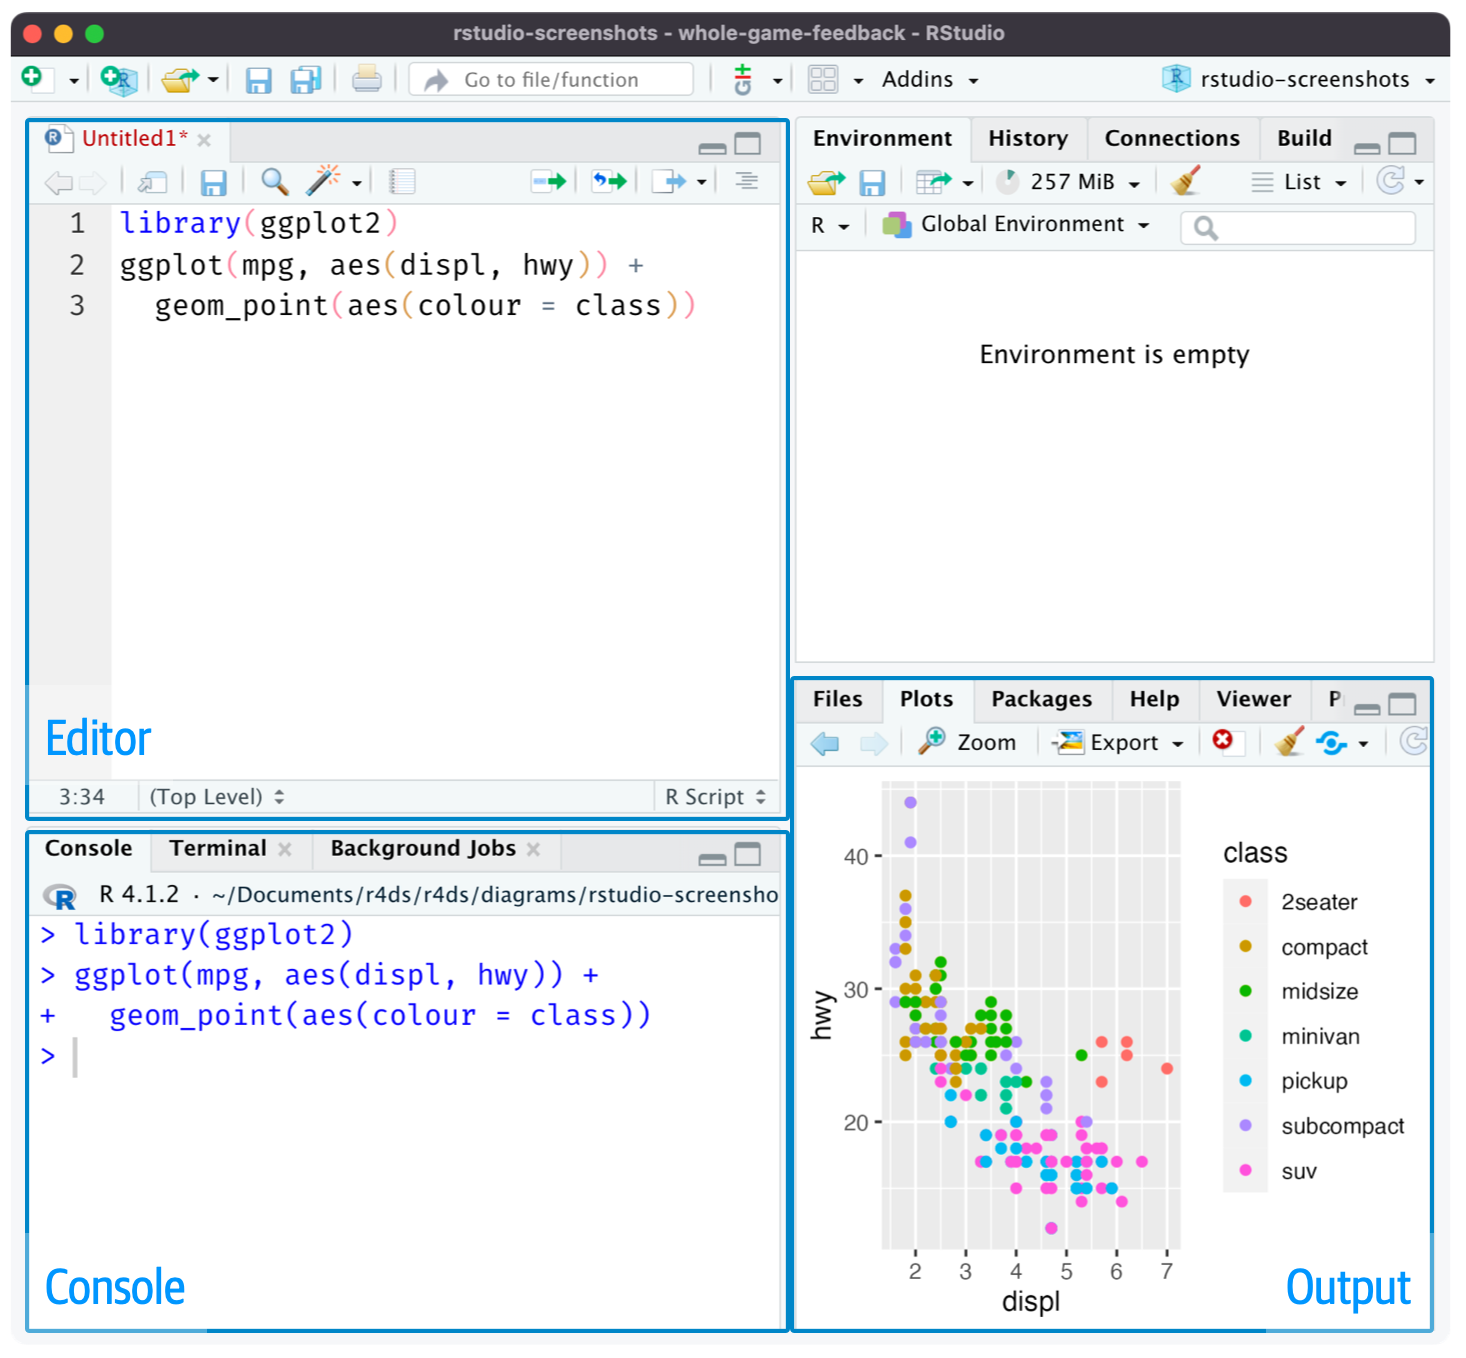
\includegraphics[width=5.43in,height=\textheight]{diagrams/rstudio/script.png}

}

\caption{\label{fig-rstudio-script}Opening the script editor adds a new
pane at the top-left of the IDE.}

\end{figure}%

\subsection{运行代码}\label{ux8fd0ux884cux4ee3ux7801}

脚本编辑器是构建复杂的ggplot2图形或长序列的dplyr操作的好地方。有
效使用脚本编辑器的关键是记住一个最重要的键盘快捷键:Cmd/Ctrl + Enter。这
个快捷键可以在控制台中执行当前的R表达式。例 如,请看下面的代码。

\begin{Shaded}
\begin{Highlighting}[]
\FunctionTok{library}\NormalTok{(dplyr)}
\FunctionTok{library}\NormalTok{(nycflights13)}

\NormalTok{not\_cancelled }\OtherTok{\textless{}{-}}\NormalTok{ flights }\SpecialCharTok{|\textgreater{}} 
  \FunctionTok{filter}\NormalTok{(}\SpecialCharTok{!}\FunctionTok{is.na}\NormalTok{(dep\_delay)█, }\SpecialCharTok{!}\FunctionTok{is.na}\NormalTok{(arr\_delay))}

\NormalTok{not\_cancelled }\SpecialCharTok{|\textgreater{}} 
  \FunctionTok{group\_by}\NormalTok{(year, month, day) }\SpecialCharTok{|\textgreater{}} 
  \FunctionTok{summarize}\NormalTok{(}\AttributeTok{mean =} \FunctionTok{mean}\NormalTok{(dep\_delay))}
\end{Highlighting}
\end{Shaded}

如果你的光标位于█处,按下Cmd/Ctrl +
Enter将运行生成\texttt{not\_cancelled}的完整命令。同
时,光标也会移动到下一个语句(以\texttt{not\_cancelled\ \textbar{}\textgreater{}}开头)。这
使得通过反复按下Cmd/Ctrl + Enter来逐步执行整个脚本变得很容易。

与其逐个表达式地运行代码,还可以使用Cmd/Ctrl + Shift +
S一次性执行完整的脚本。定
期这样做是保证你捕获了脚本中代码所有重要部分的好方法。

我们建议你始终在脚本开头列出所需的包。这
样,如果与他人共享代码,他们可以轻松地看到他们需要安装哪些包。但
是,请注意,不要在共享的脚本中包含\texttt{install.packages()}。如
果不小心将一个会更改计算机的脚本交给他们是欠考虑的!

在学习后续章节时,我们强烈推荐从脚本编辑器开始并练习您的键盘快捷键。随
着时间的推移,以这种方式将代码发送到控制台会变得如此自然,甚至不用去考虑。

\subsection{RStudio 诊断}\label{rstudio-ux8bcaux65ad}

在脚本编辑器中,RStudio会在侧边栏中用一条红色弯弯曲曲的线和一个叉来突出显示语法错误。

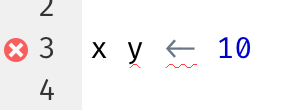
\includegraphics[width=0.49in,height=\textheight]{screenshots/rstudio-diagnostic.png}

将鼠标悬停在十字上,看看问题是什么:

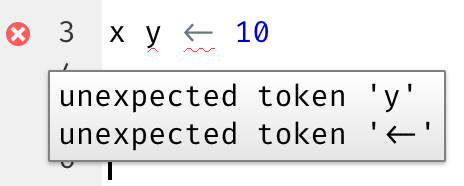
\includegraphics[width=0.77in,height=\textheight]{screenshots/rstudio-diagnostic-tip.png}

RStudio 还会让您了解潜在的问题:

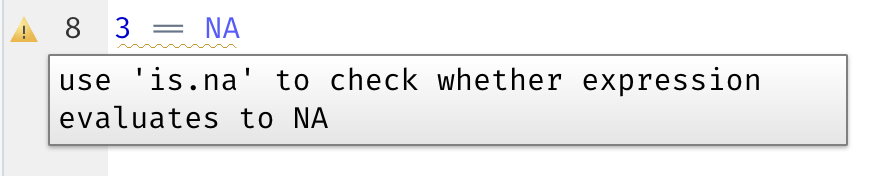
\includegraphics[width=1.46in,height=\textheight]{screenshots/rstudio-diagnostic-warn.png}

\subsection{文件保存和命名}\label{ux6587ux4ef6ux4fddux5b58ux548cux547dux540d}

RStudio
在你退出时会自动保存脚本编辑器的内容,并在重新打开时自动加载它。然
而,最好不要使用``Untitled1'',``Untitled2'',``Untitled3''等命名方式,而是应该保存您的脚本并给它们起一个有意义的名字。

可能你会想用\texttt{code.R}或\texttt{myscript.R}来命名文件,但在选择文件名之前应该多考虑一下。文
件命名的三个重要原则是:

\begin{enumerate}
\def\labelenumi{\arabic{enumi}.}
\tightlist
\item
  文件名应该是\textbf{机器}可读的:避免空格、符号和特殊字符,不要依赖大小写来区分文件。
\item
  文件名应该是\textbf{人类}可读的:使用文件名来描述文件中的内容。
\item
  文件名应该与默认排序方式兼容:以数字开头命名文件,以便按字母顺序排序时,它们能按照使用的顺序排列。
\end{enumerate}

例如,假设您在一个项目文件夹中有以下文件:

\begin{verbatim}
alternative model.R
code for exploratory analysis.r
finalreport.qmd
FinalReport.qmd
fig 1.png
Figure_02.png
model_first_try.R
run-first.r
temp.txt
\end{verbatim}

这里存在几个问题:很难确定先运行哪个文件;文件名包含空格;有两个名称相同但大小写不同的文件(\texttt{finalreport}
与
\texttt{FinalReport}\footnote{如果你在名字中使用``final''更是在冒险😆;漫画《Piled
  Higher and
  Deeper》中有一个\href{https://phdcomics.com/comics/archive.php?comicid=1531}{关于此话题的有趣连载}。}),并且一些名称没有描述其内容(\texttt{run-first}
和 \texttt{temp})。

下面是一种更好的命名和组织同一组文件的方法:

\begin{verbatim}
01-load-data.R
02-exploratory-analysis.R
03-model-approach-1.R
04-model-approach-2.R
fig-01.png
fig-02.png
report-2022-03-20.qmd
report-2022-04-02.qmd
report-draft-notes.txt
\end{verbatim}

对关键脚本进行编号可以明确它们的运行顺序,而一致的命名方案可以更容易地看出发生了什么变化。此
外,图表的标签也类似;报告通过文件名中包含的日期进行区分,而\texttt{temp}被重命名为\texttt{report-draft-notes}以更好地描述其内容。如
果您在目录中有大量文件,建议进一步组织文件,将不同类型的文件(脚本、图表等)放在不同的目录中。

\section{项目}\label{ux9879ux76ee}

有时,你可能需要退出R去做其他的事情,稍后再回到分析任务中;有时,你会同时处理多个任务,并且希望将它们分开。有
时,你需要将外部世界的数据带入R,并将R中的数值结果和图表发送回外部世界。

为了处理这些实际情况,你需要做出两个决定:

\begin{enumerate}
\def\labelenumi{\arabic{enumi}.}
\tightlist
\item
  什么是真相的来源?你会保存什么作为发生的事情的永久记录?
\item
  你的分析在哪里进行?
\end{enumerate}

\subsection{什么是真相的来源?}\label{ux4ec0ux4e48ux662fux771fux76f8ux7684ux6765ux6e90}

作为初学者,依靠当前环境(Environment
)包含分析过程中创建的所有对象是无可厚非的。但
是,为了更容易地进行大型项目或与他人合作,R脚本应该成为事实真相的来源,你可以通过R脚本(和数据文件)重新创建环境。如
果只有自己的环境,则很难重新创建R脚本:你要么必须从记忆中重新键入大量代码(在此过程中不可避免地会犯错误),要么必须仔细挖掘您的R历史记录。

为了帮助保持R脚本作为你分析的真相来源,我们强烈建议你不要让RStudio在会话之间保留您的工作空间(workspace)。您
可以通过运行\texttt{usethis::use\_blank\_slate()}\footnote{如果没有安装usethis,可以使用\texttt{install.packages("usethis")}安装。}或模仿
图~\ref{fig-blank-slate} 中所示的选项来实现。
这将会给您带来一些短期的痛苦,因为现在当您重新启动RStudio时,它将不再记住您上次运行的代码,您创建的对象或读取的数据集也将无法使用。
但是这种短期的痛苦可以避免长期的痛苦,因为它迫使你在代码中捕获所有重要的过程。
没有什么比在事实发生三个月后发现你只在环境中存储了重要计算的结果,而没有在代码中存储计算更糟糕的了。

\begin{figure}

\centering{

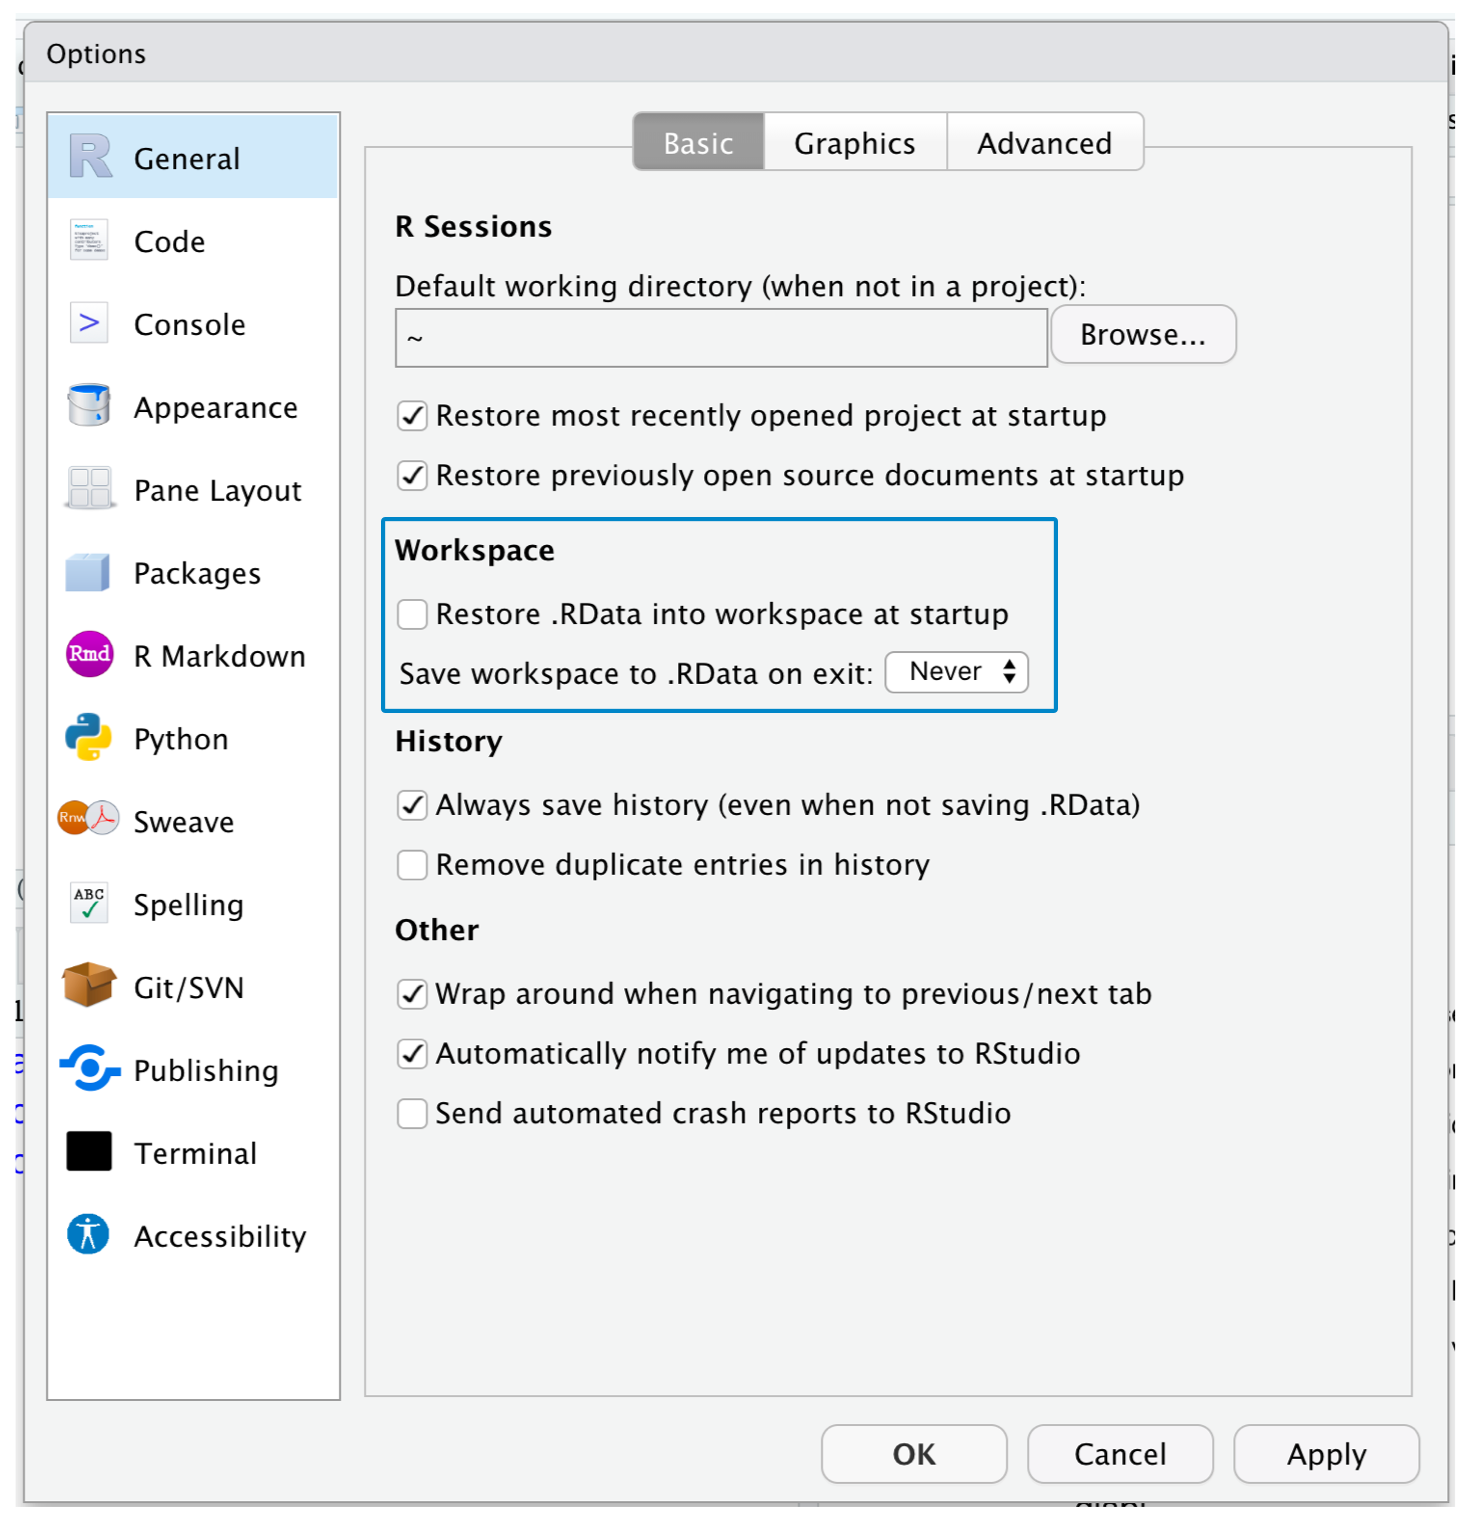
\includegraphics[width=5.44in,height=\textheight]{diagrams/rstudio/clean-slate.png}

}

\caption{\label{fig-blank-slate}Copy these options in your RStudio
options to always start your RStudio session with a clean slate.}

\end{figure}%

有一组非常实用的键盘快捷键组合,它们将协同工作以确保你已经在编辑器中捕获了代码的重要部分:

\begin{enumerate}
\def\labelenumi{\arabic{enumi}.}
\tightlist
\item
  按Cmd/Ctrl + Shift + 0/F10来重启R。
\item
  按Cmd/Ctrl + Shift + S来重新运行当前脚本。
\end{enumerate}

我们每周都会使用这种模式数百次。

或者,如果不使用快捷键,你可以转到``会话''\textgreater{}``重启R'',然后选中并重新运行当前脚本。

\begin{tcolorbox}[enhanced jigsaw, colbacktitle=quarto-callout-note-color!10!white, breakable, opacityback=0, title=\textcolor{quarto-callout-note-color}{\faInfo}\hspace{0.5em}{RStudio server}, toprule=.15mm, leftrule=.75mm, colback=white, coltitle=black, rightrule=.15mm, opacitybacktitle=0.6, titlerule=0mm, arc=.35mm, bottomtitle=1mm, colframe=quarto-callout-note-color-frame, toptitle=1mm, bottomrule=.15mm, left=2mm]

如果您使用的是RStudio server,默认情况下R会话不会自动重启。当
你关闭RStudio
server标签页时,可能会感觉正在关闭R,但实际上服务器会在后台保持其运行状态。下
次你返回时,你将处于和离开时完全相同的位置。这
使得定期重启R变得尤为重要,以便你是从一个干净状态开始的。

\end{tcolorbox}

\subsection{分析在哪里进行?}\label{ux5206ux6790ux5728ux54eaux91ccux8fdbux884c}

\textbf{工作目录}是R中非常重要的概念。R
在这个目录中查找你想要加载的文件,也将要保存的文件存放在这里。R
Studio在控制台顶部显示当前的工作目录:

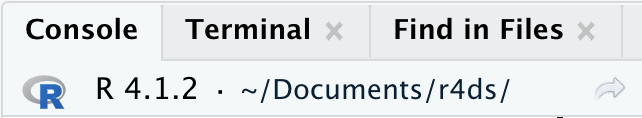
\includegraphics[width=1.07in,height=\textheight]{screenshots/rstudio-wd.png}

可以通过运行\texttt{getwd()}函数在R代码中输出当前的工作目录:

\begin{Shaded}
\begin{Highlighting}[]
\FunctionTok{getwd}\NormalTok{()}
\CommentTok{\#\textgreater{} [1] "/Users/hadley/Documents/r4ds"}
\end{Highlighting}
\end{Shaded}

本次R会话中,当前工作目录(可以将其视为``主目录'')位于Hadley的Documents文件夹中一个名为r4ds的子文件夹中。当
您运行此代码时,它将返回不同的结果,因为你的计算机的目录结构与Hadley的不同!

作为R的初学者,让工作目录成为你的主目录、文档目录或者计算机上的任何其他奇怪的目录都是可以的。但
是,你已经阅读了本书中的多个章节,不再是初学者了。现
在,你应该开始将项目组织到目录中,并在处理项目时将R的工作目录设置为相关目录。

你可以在R内部设置工作目录,但\textbf{不推荐这样做}:

\begin{Shaded}
\begin{Highlighting}[]
\FunctionTok{setwd}\NormalTok{(}\StringTok{"/path/to/my/CoolProject"}\NormalTok{)}
\end{Highlighting}
\end{Shaded}

有一种更好的方法,这种方法也能让您像专家一样管理R工作。那
就是使用RStudio项目。

\subsection{RStudio项目}\label{rstudioux9879ux76ee}

将所有与某个项目相关的文件(输入数据、R脚本、分析结果和图表)保存在一个目录中是一种明智且常见的做法,RStudio通过项目提供了内置支持。让
我们为您创建一个项目,以便您在使用本书的其余部分时可以使用它。点
击``文件''\textgreater{}``新建项目'',然后按照@fig-new-project
中显示的步骤操作。

\begin{figure}

\centering{

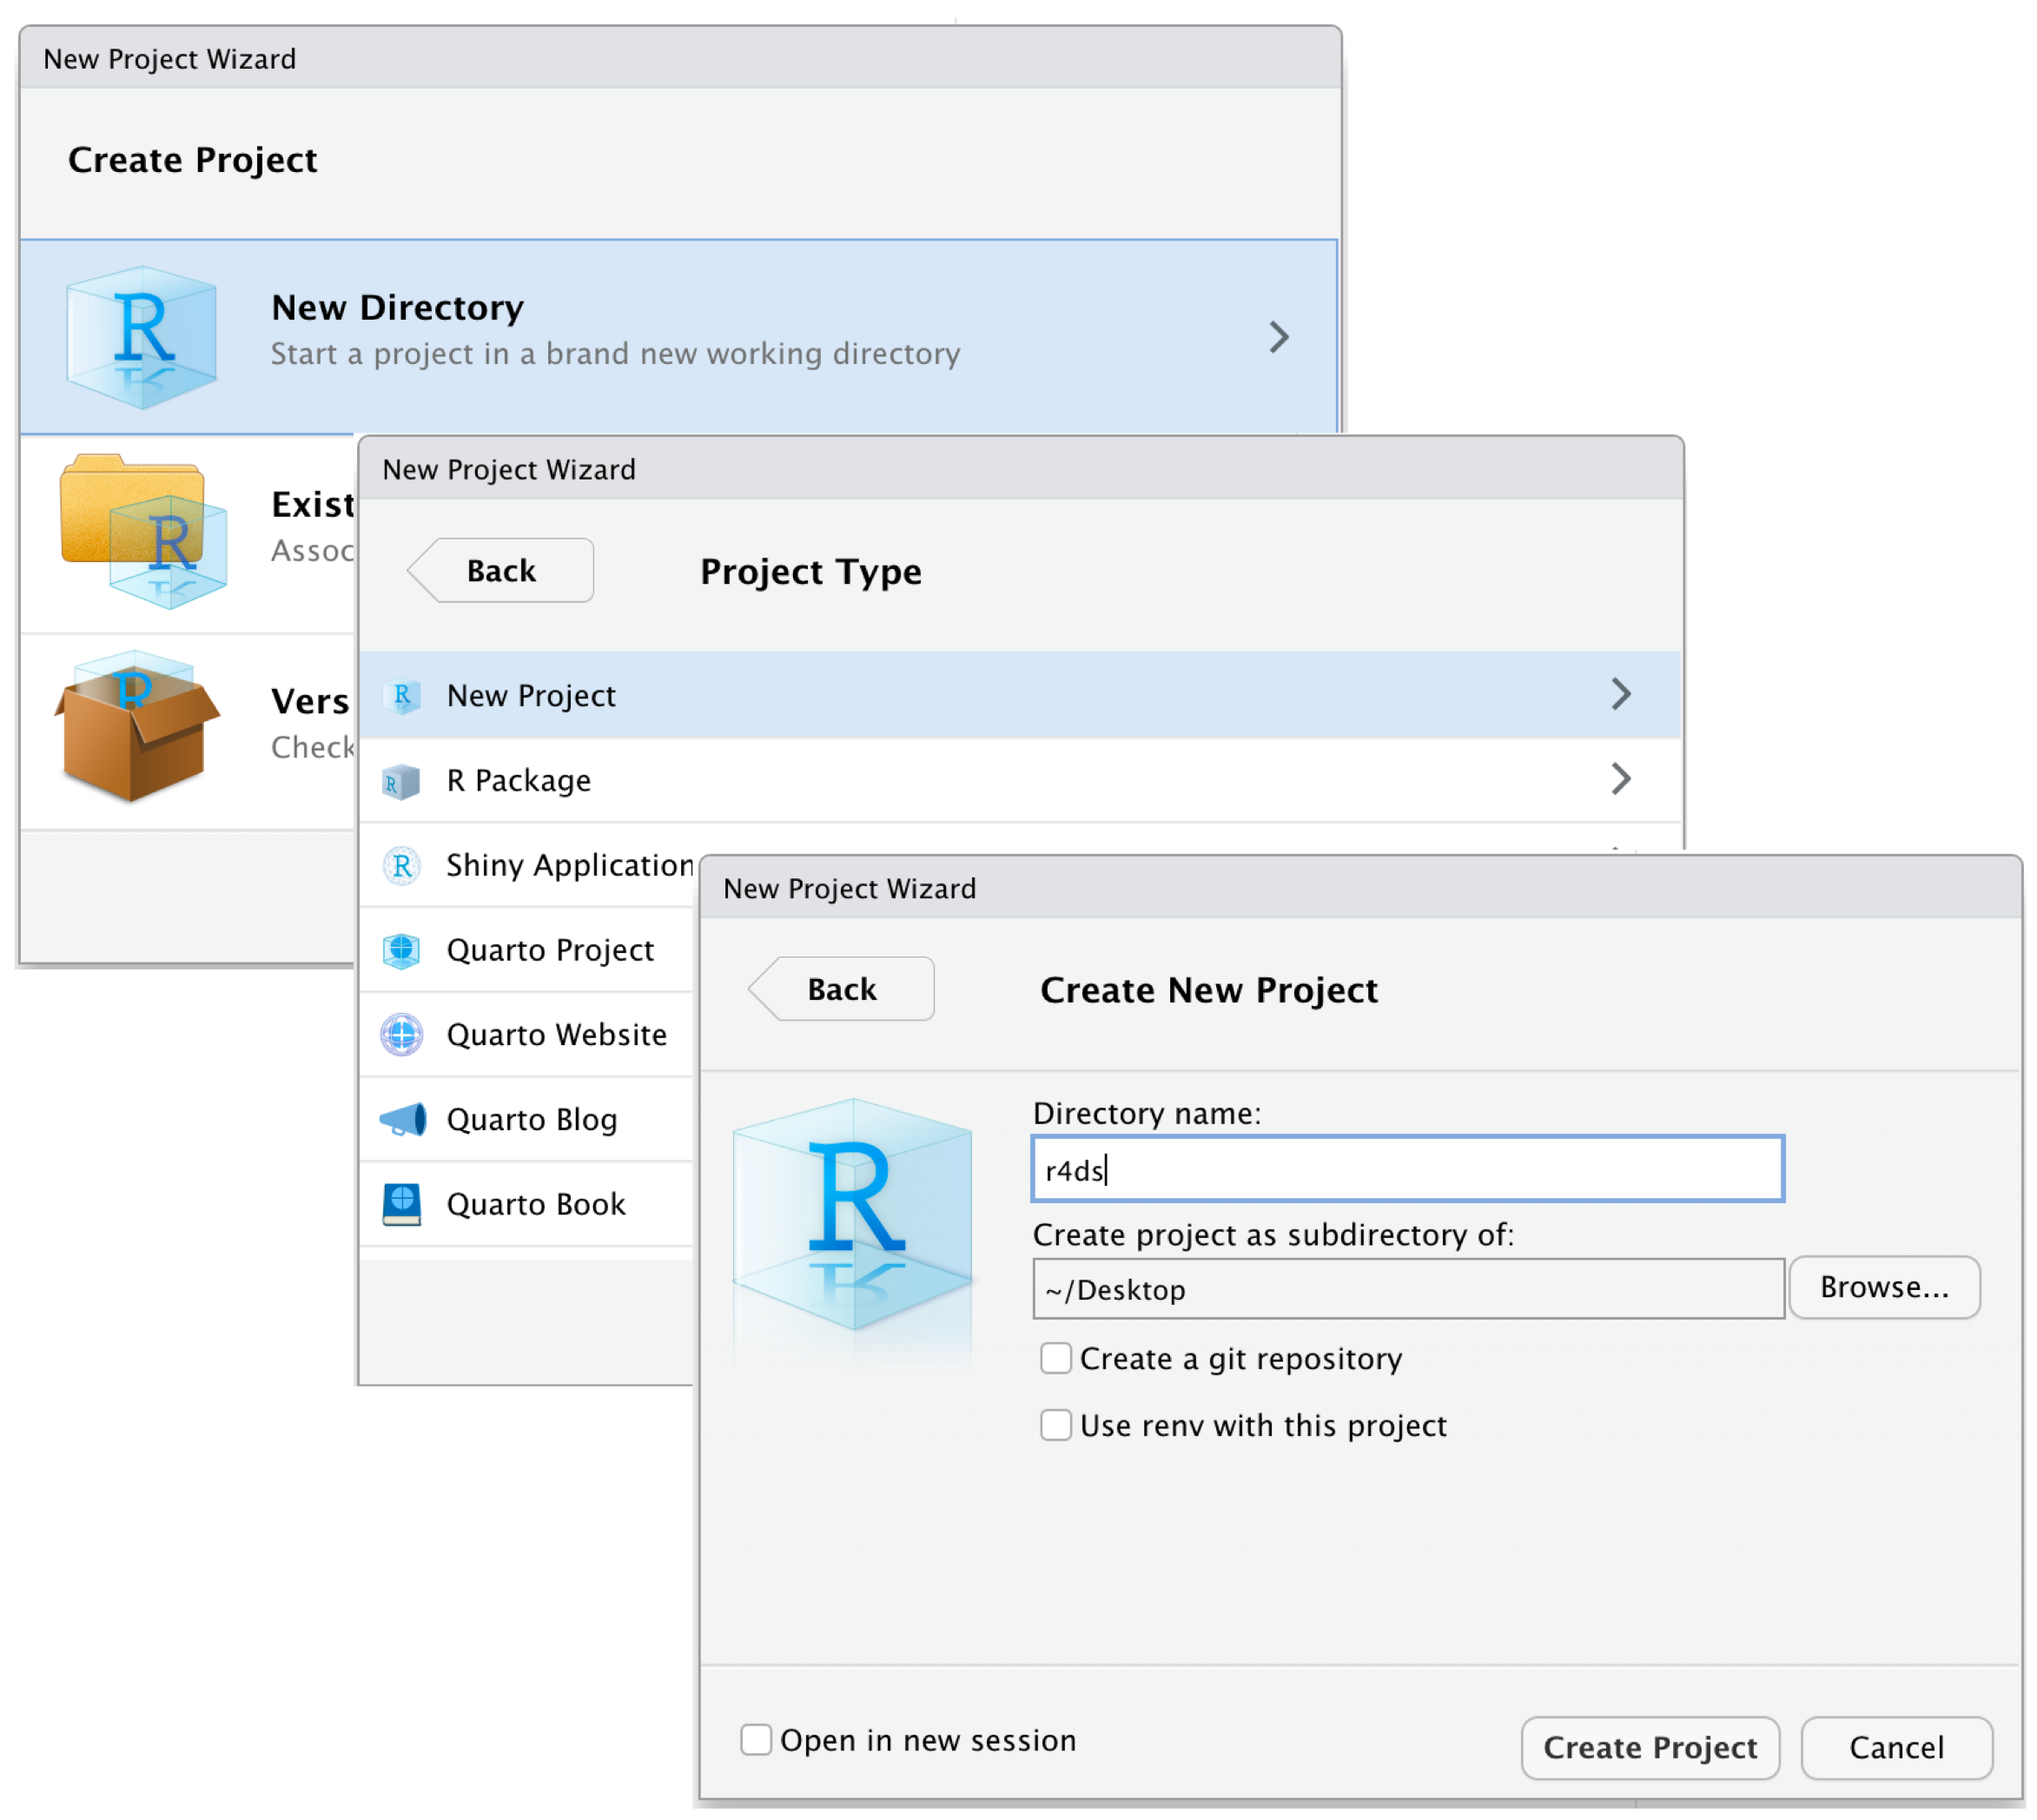
\includegraphics[width=3.91in,height=\textheight]{diagrams/new-project.png}

}

\caption{\label{fig-new-project}To create new project: (top) first click
New Directory, then (middle) click New Project, then (bottom) fill in
the directory (project) name, choose a good subdirectory for its home
and click Create Project.}

\end{figure}%

将你的项目命名为\texttt{r4ds},并仔细考虑将其放在哪个子目录中。如
果不将其存储在一个合理的地方,将来会很难找到它!

一旦完成此过程,你将获得一个专为此书创建的新RStudio项目。请
检查项目的``主目录''是否已设置为当前工作目录:

\begin{Shaded}
\begin{Highlighting}[]
\FunctionTok{getwd}\NormalTok{()}
\CommentTok{\#\textgreater{} [1] /Users/hadley/Documents/r4ds}
\end{Highlighting}
\end{Shaded}

现在,在脚本编辑器中输入以下命令并将文件保存为``diamonds.R''。然
后,创建一个名为``data''的新文件夹。你
可以通过在RStudio的``文件''面板中点击``新建文件夹''按钮来完成此操作。最
后,运行完整的脚本,它将把PNG和CSV文件保存到您的项目目录中。不
用关注细节,你将在本书的后续中学习它们。

\begin{Shaded}
\begin{Highlighting}[]
\FunctionTok{library}\NormalTok{(tidyverse)}

\FunctionTok{ggplot}\NormalTok{(diamonds, }\FunctionTok{aes}\NormalTok{(}\AttributeTok{x =}\NormalTok{ carat, }\AttributeTok{y =}\NormalTok{ price)) }\SpecialCharTok{+} 
  \FunctionTok{geom\_hex}\NormalTok{()}
\FunctionTok{ggsave}\NormalTok{(}\StringTok{"diamonds.png"}\NormalTok{)}

\FunctionTok{write\_csv}\NormalTok{(diamonds, }\StringTok{"data/diamonds.csv"}\NormalTok{)}
\end{Highlighting}
\end{Shaded}

退出RStudio。检
查与你的项目关联的文件夹------注意\texttt{.Rproj}文件。双
击该文件以重新打开项目。请
注意,你回到了离开时的位置:工作目录和命令历史与原来相同,你正在处理的所有文件仍然打开。但
是,由于遵循了上面的说明,你将拥有一个全新的环境,确保你是从一个干净的状态开始的。

根据操作系统的不同,选择你最喜欢的方式在计算机上搜索\texttt{diamonds.png}。你
会找到PNG文件(这并不奇怪),还会找到创建它的脚本文件\texttt{diamonds.R}。这
是一个巨大的胜利!有
一天,你可能会想要重新生成一个图形或只是了解它的来源。如
果你严格地使用R代码将图形保存到文件中而从不使用鼠标或剪贴板,那么你将能够轻松地重复以前的工作!

\subsection{相对和绝对路径}\label{ux76f8ux5bf9ux548cux7eddux5bf9ux8defux5f84}

一旦进入一个项目,你应该只使用相对路径而不是绝对路径。有 什么区别呢?相
对路径是相对于工作目录的,即项目的根目录。当
Hadley在上面写\texttt{data/diamonds.csv}时,它是\texttt{/Users/hadley/Documents/r4ds/data/diamonds.csv}的快捷方式。但
如果Mine在她的计算机上运行这段代码,它将指向\texttt{/Users/Mine/Documents/r4ds/data/diamonds.csv}。这
就是为什么相对路径很重要:无论R项目文件夹最终位于何处,它们都能正常工作。

绝对路径是指向同一个位置,与你的工作目录无关。根
据操作系统不同,它们看上去会有所不同。在
Windows上,它们以驱动器字母(例如,\texttt{C:})或两个反斜杠(例如,\texttt{\textbackslash{}\textbackslash{}servername})开头,而在Mac/Linux上,它们以斜杠``/''开头(例如,\texttt{/users/hadley})。你
不应该在脚本中使用绝对路径,因为它们会妨碍共享:没有人会拥有与你完全相同的目录配置。

操作系统之间还有一个重要的区别:如何分隔路径的各个部分。M
ac和Linux使用斜杠(例如,\texttt{data/diamonds.csv}),而Windows使用反斜杠(例如,\texttt{data\textbackslash{}diamonds.csv})。R
可以与这两种类型一起工作(无论你当前使用什么平台),但不幸的是,反斜杠在R中有特殊含义,要在路径中获得单个反斜杠,您需要键入两个反斜杠!这
会使生活变得令人沮丧,因此我们建议使用Linux/Mac风格的斜杠。

\section{练习}\label{ux7ec3ux4e60-10}

\begin{enumerate}
\def\labelenumi{\arabic{enumi}.}
\item
  登录RStudio Tips Twitter账户
  \url{https://twitter.com/rstudiotips},找到一个有趣的技巧,练习使用它!
\item
  RStudio诊断还会报告哪些常见错误?阅 读
  \url{https://support.posit.co/hc/en-us/articles/205753617-Code-Diagnostics}
  找到答案。
\end{enumerate}

\section{小结}\label{ux5c0fux7ed3-5}

在本章中,你学习了如何在脚本(文件)和项目(目录)中组织代码。就
像代码风格一样,这在一开始可能会感觉像是在做无用功。但
是,随着你在多个项目中积累更多的代码,你会开始认识到前期的一点组织工作可以为你节省大量的时间。

总的来说,脚本和项目为你提供了一个坚实的工作流程,这会在未来很好地为你服务:

\begin{itemize}
\tightlist
\item
  为每个数据分析项目创建一个RStudio项目;
\item
  在项目中保存你的脚本(起一个带有信息的名字),编辑它们,分部分或整体运行它们;经常重新启动R以确保你已将所有内容捕获到脚本中。
\item
  永远只使用相对路径,而不是绝对路径。
\end{itemize}

然后,你需要的所有内容都存放于一个地方,并且与您正在处理的所有其他项目干净地分隔开。

到目前为止,我们一直在使用R包中包含的数据集。这
使得在预先准备的数据上进行一些实践变得更容易,但显然你的数据不会以这种方式提供。因
此,在下一章中将学习如何使用readr包将数据从磁盘加载到R会话中。

\chapter{数据导入}\label{sec-data-import}

\section{引言}\label{ux5f15ux8a00-3}

使用R包提供的数据来学习数据科学工具是一个很好的方法,但总有一天你会想将所学应用于自己的数据。在
本章中,你将学习将数据文件读入R的基础知识。

具体来说,本章将重点关注读取纯文本矩形文件。我
们将从处理列名、类型和缺失数据的实用建议开始。然
后,学习如何一次从多个文件中读取数据,以及如何将R中的数据写入文件。最
后,学习如何在R中手动创建数据框。

\subsection{必要条件}\label{ux5fc5ux8981ux6761ux4ef6-3}

在本章中,你将学习如何使用\textbf{readr}包在R中加载平面文件,readr包是核心包tidyverse的一部分。

\begin{Shaded}
\begin{Highlighting}[]
\FunctionTok{library}\NormalTok{(tidyverse)}
\end{Highlighting}
\end{Shaded}

\section{从文件读取数据}\label{ux4eceux6587ux4ef6ux8bfbux53d6ux6570ux636e}

首先,我们将关注最常见的矩形数据文件类型:CSV(Comma-Separated
Values的缩写)。下
面是一个简单的CSV文件,第一行通常被称为标题行,给出了列名,接下来的六行提供了数据,列之间由逗号分隔,也称为定界符。

\begin{verbatim}
Student ID,Full Name,favourite.food,mealPlan,AGE
1,Sunil Huffmann,Strawberry yoghurt,Lunch only,4
2,Barclay Lynn,French fries,Lunch only,5
3,Jayendra Lyne,N/A,Breakfast and lunch,7
4,Leon Rossini,Anchovies,Lunch only,
5,Chidiegwu Dunkel,Pizza,Breakfast and lunch,five
6,Güvenç Attila,Ice cream,Lunch only,6
\end{verbatim}

表~\ref{tbl-students-table} 以表格形式呈现了相同的数据。

\begin{longtable}[]{@{}
  >{\raggedleft\arraybackslash}p{(\columnwidth - 8\tabcolsep) * \real{0.1528}}
  >{\raggedright\arraybackslash}p{(\columnwidth - 8\tabcolsep) * \real{0.2361}}
  >{\raggedright\arraybackslash}p{(\columnwidth - 8\tabcolsep) * \real{0.2639}}
  >{\raggedright\arraybackslash}p{(\columnwidth - 8\tabcolsep) * \real{0.2778}}
  >{\raggedright\arraybackslash}p{(\columnwidth - 8\tabcolsep) * \real{0.0694}}@{}}

\caption{\label{tbl-students-table}Data from the students.csv file as a
table.}

\tabularnewline

\toprule\noalign{}
\begin{minipage}[b]{\linewidth}\raggedleft
Student ID
\end{minipage} & \begin{minipage}[b]{\linewidth}\raggedright
Full Name
\end{minipage} & \begin{minipage}[b]{\linewidth}\raggedright
favourite.food
\end{minipage} & \begin{minipage}[b]{\linewidth}\raggedright
mealPlan
\end{minipage} & \begin{minipage}[b]{\linewidth}\raggedright
AGE
\end{minipage} \\
\midrule\noalign{}
\endhead
\bottomrule\noalign{}
\endlastfoot
1 & Sunil Huffmann & Strawberry yoghurt & Lunch only & 4 \\
2 & Barclay Lynn & French fries & Lunch only & 5 \\
3 & Jayendra Lyne & N/A & Breakfast and lunch & 7 \\
4 & Leon Rossini & Anchovies & Lunch only & NA \\
5 & Chidiegwu Dunkel & Pizza & Breakfast and lunch & five \\
6 & Güvenç Attila & Ice cream & Lunch only & 6 \\

\end{longtable}

我们使用\texttt{read\_csv()}将这个文件读入R。第
一个参数是最重要的:文件路径。可
以将路径视为文件的地址,文件名为\texttt{students.csv},它位于\texttt{data}文件夹中。

\begin{Shaded}
\begin{Highlighting}[]
\NormalTok{students }\OtherTok{\textless{}{-}} \FunctionTok{read\_csv}\NormalTok{(}\StringTok{"data/students.csv"}\NormalTok{)}
\CommentTok{\#\textgreater{} Rows: 6 Columns: 5}
\CommentTok{\#\textgreater{} {-}{-} Column specification {-}{-}{-}{-}{-}{-}{-}{-}{-}{-}{-}{-}{-}{-}{-}{-}{-}{-}{-}{-}{-}{-}{-}{-}{-}{-}{-}{-}{-}{-}{-}{-}{-}{-}{-}{-}{-}{-}{-}{-}{-}{-}{-}{-}{-}{-}{-}{-}{-}{-}{-}{-}{-}}
\CommentTok{\#\textgreater{} Delimiter: ","}
\CommentTok{\#\textgreater{} chr (4): Full Name, favourite.food, mealPlan, AGE}
\CommentTok{\#\textgreater{} dbl (1): Student ID}
\CommentTok{\#\textgreater{} }
\CommentTok{\#\textgreater{} i Use \textasciigrave{}spec()\textasciigrave{} to retrieve the full column specification for this data.}
\CommentTok{\#\textgreater{} i Specify the column types or set \textasciigrave{}show\_col\_types = FALSE\textasciigrave{} to quiet this message.}
\end{Highlighting}
\end{Shaded}

上面的代码在你的项目中存在名为 \texttt{data} 的文件夹并且其中包含
\texttt{students.csv} 文件时有效。您
可以从\url{https://pos.it/r4ds-students-csv}下载 \texttt{students.csv}
文件,或者可以直接从该URL读取它,使用如下方式:

\begin{Shaded}
\begin{Highlighting}[]
\NormalTok{students }\OtherTok{\textless{}{-}} \FunctionTok{read\_csv}\NormalTok{(}\StringTok{"https://pos.it/r4ds{-}students{-}csv"}\NormalTok{)}
\end{Highlighting}
\end{Shaded}

当你运行\texttt{read\_csv()}时,它会输出一条消息,告诉你数据的行数和列数、所使用的分隔符以及列规范(按列中数据类型组织的列名)。它
还会输出关于如何检索完整列规范和如何静默此消息的一些信息。这
条消息是\texttt{readr}包的一个组成部分,我们将在@sec-col-types
中再次讨论它。

\subsection{实用建议}\label{ux5b9eux7528ux5efaux8bae}

一旦你读取了数据,第一步通常是以某种方式转换它,以使其在剩余的分析中更容易处理。让
我们带着这个想法再次查看\texttt{students}数据。

\begin{Shaded}
\begin{Highlighting}[]
\NormalTok{students}
\CommentTok{\#\textgreater{} \# A tibble: 6 x 5}
\CommentTok{\#\textgreater{}   \textasciigrave{}Student ID\textasciigrave{} \textasciigrave{}Full Name\textasciigrave{}      favourite.food     mealPlan            AGE  }
\CommentTok{\#\textgreater{}          \textless{}dbl\textgreater{} \textless{}chr\textgreater{}            \textless{}chr\textgreater{}              \textless{}chr\textgreater{}               \textless{}chr\textgreater{}}
\CommentTok{\#\textgreater{} 1            1 Sunil Huffmann   Strawberry yoghurt Lunch only          4    }
\CommentTok{\#\textgreater{} 2            2 Barclay Lynn     French fries       Lunch only          5    }
\CommentTok{\#\textgreater{} 3            3 Jayendra Lyne    N/A                Breakfast and lunch 7    }
\CommentTok{\#\textgreater{} 4            4 Leon Rossini     Anchovies          Lunch only          \textless{}NA\textgreater{} }
\CommentTok{\#\textgreater{} 5            5 Chidiegwu Dunkel Pizza              Breakfast and lunch five }
\CommentTok{\#\textgreater{} 6            6 Güvenç Attila    Ice cream          Lunch only          6}
\end{Highlighting}
\end{Shaded}

在\texttt{favourite.food}列中有一堆食品项目,然后是字符串\texttt{N/A},它应该是一个
R 会识别为``不可用''的真正的\texttt{NA}值。这
是我们可以通过\texttt{na}参数来解决的问题。默
认情况下,\texttt{read\_csv()}只将此数据集中的空字符串(\texttt{""})
识别为 \texttt{NA}s,我们希望它也能识别字符串\texttt{"N/A"}。

\begin{Shaded}
\begin{Highlighting}[]
\NormalTok{students }\OtherTok{\textless{}{-}} \FunctionTok{read\_csv}\NormalTok{(}\StringTok{"data/students.csv"}\NormalTok{, }\AttributeTok{na =} \FunctionTok{c}\NormalTok{(}\StringTok{"N/A"}\NormalTok{, }\StringTok{""}\NormalTok{))}

\NormalTok{students}
\CommentTok{\#\textgreater{} \# A tibble: 6 x 5}
\CommentTok{\#\textgreater{}   \textasciigrave{}Student ID\textasciigrave{} \textasciigrave{}Full Name\textasciigrave{}      favourite.food     mealPlan            AGE  }
\CommentTok{\#\textgreater{}          \textless{}dbl\textgreater{} \textless{}chr\textgreater{}            \textless{}chr\textgreater{}              \textless{}chr\textgreater{}               \textless{}chr\textgreater{}}
\CommentTok{\#\textgreater{} 1            1 Sunil Huffmann   Strawberry yoghurt Lunch only          4    }
\CommentTok{\#\textgreater{} 2            2 Barclay Lynn     French fries       Lunch only          5    }
\CommentTok{\#\textgreater{} 3            3 Jayendra Lyne    \textless{}NA\textgreater{}               Breakfast and lunch 7    }
\CommentTok{\#\textgreater{} 4            4 Leon Rossini     Anchovies          Lunch only          \textless{}NA\textgreater{} }
\CommentTok{\#\textgreater{} 5            5 Chidiegwu Dunkel Pizza              Breakfast and lunch five }
\CommentTok{\#\textgreater{} 6            6 Güvenç Attila    Ice cream          Lunch only          6}
\end{Highlighting}
\end{Shaded}

你可能还注意到,\texttt{Student\ ID}和\texttt{Full\ Name}列使用了反引号。这
是因为它们包含空格,违反了 R
中变量名的常规规则,它们是非语法(\textbf{non-syntactic})名称。要
引用这些变量,你需要使用反引号\texttt{\textasciigrave{}}将它们括起来。

\begin{Shaded}
\begin{Highlighting}[]
\NormalTok{students }\SpecialCharTok{|\textgreater{}} 
  \FunctionTok{rename}\NormalTok{(}
    \AttributeTok{student\_id =} \StringTok{\textasciigrave{}}\AttributeTok{Student ID}\StringTok{\textasciigrave{}}\NormalTok{,}
    \AttributeTok{full\_name =} \StringTok{\textasciigrave{}}\AttributeTok{Full Name}\StringTok{\textasciigrave{}}
\NormalTok{  )}
\CommentTok{\#\textgreater{} \# A tibble: 6 x 5}
\CommentTok{\#\textgreater{}   student\_id full\_name        favourite.food     mealPlan            AGE  }
\CommentTok{\#\textgreater{}        \textless{}dbl\textgreater{} \textless{}chr\textgreater{}            \textless{}chr\textgreater{}              \textless{}chr\textgreater{}               \textless{}chr\textgreater{}}
\CommentTok{\#\textgreater{} 1          1 Sunil Huffmann   Strawberry yoghurt Lunch only          4    }
\CommentTok{\#\textgreater{} 2          2 Barclay Lynn     French fries       Lunch only          5    }
\CommentTok{\#\textgreater{} 3          3 Jayendra Lyne    \textless{}NA\textgreater{}               Breakfast and lunch 7    }
\CommentTok{\#\textgreater{} 4          4 Leon Rossini     Anchovies          Lunch only          \textless{}NA\textgreater{} }
\CommentTok{\#\textgreater{} 5          5 Chidiegwu Dunkel Pizza              Breakfast and lunch five }
\CommentTok{\#\textgreater{} 6          6 Güvenç Attila    Ice cream          Lunch only          6}
\end{Highlighting}
\end{Shaded}

另一种方法是使用~\texttt{janitor::clean\_names()}~函数,该函数使用一些启发式方法来一次性将它们全部转换为蛇形命名法(snake
case)\footnote{\href{http://sfirke.github.io/janitor/}{janitor}包不是tidyverse的一部分,但它提供了方便的数据清理功能,并且在使用\texttt{\textbar{}\textgreater{}}的数据管道中工作得很好。}。

\begin{Shaded}
\begin{Highlighting}[]
\NormalTok{students }\SpecialCharTok{|\textgreater{}}\NormalTok{ janitor}\SpecialCharTok{::}\FunctionTok{clean\_names}\NormalTok{()}
\CommentTok{\#\textgreater{} \# A tibble: 6 x 5}
\CommentTok{\#\textgreater{}   student\_id full\_name        favourite\_food     meal\_plan           age  }
\CommentTok{\#\textgreater{}        \textless{}dbl\textgreater{} \textless{}chr\textgreater{}            \textless{}chr\textgreater{}              \textless{}chr\textgreater{}               \textless{}chr\textgreater{}}
\CommentTok{\#\textgreater{} 1          1 Sunil Huffmann   Strawberry yoghurt Lunch only          4    }
\CommentTok{\#\textgreater{} 2          2 Barclay Lynn     French fries       Lunch only          5    }
\CommentTok{\#\textgreater{} 3          3 Jayendra Lyne    \textless{}NA\textgreater{}               Breakfast and lunch 7    }
\CommentTok{\#\textgreater{} 4          4 Leon Rossini     Anchovies          Lunch only          \textless{}NA\textgreater{} }
\CommentTok{\#\textgreater{} 5          5 Chidiegwu Dunkel Pizza              Breakfast and lunch five }
\CommentTok{\#\textgreater{} 6          6 Güvenç Attila    Ice cream          Lunch only          6}
\end{Highlighting}
\end{Shaded}

读取数据后的另一个常见任务是考虑变量类型。例
如,\texttt{meal\_plan}是一个分类变量,具有一组已知的可能值,在 R
中应该表示为因子:

\begin{Shaded}
\begin{Highlighting}[]
\NormalTok{students }\SpecialCharTok{|\textgreater{}}
\NormalTok{  janitor}\SpecialCharTok{::}\FunctionTok{clean\_names}\NormalTok{() }\SpecialCharTok{|\textgreater{}}
  \FunctionTok{mutate}\NormalTok{(}\AttributeTok{meal\_plan =} \FunctionTok{factor}\NormalTok{(meal\_plan))}
\CommentTok{\#\textgreater{} \# A tibble: 6 x 5}
\CommentTok{\#\textgreater{}   student\_id full\_name        favourite\_food     meal\_plan           age  }
\CommentTok{\#\textgreater{}        \textless{}dbl\textgreater{} \textless{}chr\textgreater{}            \textless{}chr\textgreater{}              \textless{}fct\textgreater{}               \textless{}chr\textgreater{}}
\CommentTok{\#\textgreater{} 1          1 Sunil Huffmann   Strawberry yoghurt Lunch only          4    }
\CommentTok{\#\textgreater{} 2          2 Barclay Lynn     French fries       Lunch only          5    }
\CommentTok{\#\textgreater{} 3          3 Jayendra Lyne    \textless{}NA\textgreater{}               Breakfast and lunch 7    }
\CommentTok{\#\textgreater{} 4          4 Leon Rossini     Anchovies          Lunch only          \textless{}NA\textgreater{} }
\CommentTok{\#\textgreater{} 5          5 Chidiegwu Dunkel Pizza              Breakfast and lunch five }
\CommentTok{\#\textgreater{} 6          6 Güvenç Attila    Ice cream          Lunch only          6}
\end{Highlighting}
\end{Shaded}

请注意,\texttt{meal\_plan}变量中的值保持不变,但变量名下方表示的变量类型已经从字符型(\texttt{\textless{}chr}\textgreater)变为了因子型(\textless{}\texttt{fct}\textgreater)。你
将在 章节~\ref{sec-factors} 中了解更多关于因子的内容。

在分析这些数据之前,你可能想要修复\texttt{age}和\texttt{id}列。目
前,\texttt{age}是一个字符型变量,因为其中一个观测值被输入为文本\texttt{five}而不是数字\texttt{5}。我
们将在 章节~\ref{sec-import-spreadsheets} 详细讨论如何修复这个问题。

\begin{Shaded}
\begin{Highlighting}[]
\NormalTok{students }\OtherTok{\textless{}{-}}\NormalTok{ students }\SpecialCharTok{|\textgreater{}}
\NormalTok{  janitor}\SpecialCharTok{::}\FunctionTok{clean\_names}\NormalTok{() }\SpecialCharTok{|\textgreater{}}
  \FunctionTok{mutate}\NormalTok{(}
    \AttributeTok{meal\_plan =} \FunctionTok{factor}\NormalTok{(meal\_plan),}
    \AttributeTok{age =} \FunctionTok{parse\_number}\NormalTok{(}\FunctionTok{if\_else}\NormalTok{(age }\SpecialCharTok{==} \StringTok{"five"}\NormalTok{, }\StringTok{"5"}\NormalTok{, age))}
\NormalTok{  )}

\NormalTok{students}
\CommentTok{\#\textgreater{} \# A tibble: 6 x 5}
\CommentTok{\#\textgreater{}   student\_id full\_name        favourite\_food     meal\_plan             age}
\CommentTok{\#\textgreater{}        \textless{}dbl\textgreater{} \textless{}chr\textgreater{}            \textless{}chr\textgreater{}              \textless{}fct\textgreater{}               \textless{}dbl\textgreater{}}
\CommentTok{\#\textgreater{} 1          1 Sunil Huffmann   Strawberry yoghurt Lunch only              4}
\CommentTok{\#\textgreater{} 2          2 Barclay Lynn     French fries       Lunch only              5}
\CommentTok{\#\textgreater{} 3          3 Jayendra Lyne    \textless{}NA\textgreater{}               Breakfast and lunch     7}
\CommentTok{\#\textgreater{} 4          4 Leon Rossini     Anchovies          Lunch only             NA}
\CommentTok{\#\textgreater{} 5          5 Chidiegwu Dunkel Pizza              Breakfast and lunch     5}
\CommentTok{\#\textgreater{} 6          6 Güvenç Attila    Ice cream          Lunch only              6}
\end{Highlighting}
\end{Shaded}

这里有一个新的函数\texttt{if\_else()},它有三个参数。第
一个参数\texttt{test}应该是一个逻辑向量。当
\texttt{test}为\texttt{TRUE}时,结果将包含第二个参数\texttt{yes}的值;当它为\texttt{FALSE}时,将包含第三个参数\texttt{no}的值。在
这里,我们表示如果\texttt{age}是字符串 \texttt{"five"},则将其变为
\texttt{"5"},如果不是,则保持原样。你 将在 章节~\ref{sec-logicals}
部分了解更多关于\texttt{if\_else()}和逻辑向量的内容。

\subsection{其他参数}\label{ux5176ux4ed6ux53c2ux6570}

这里还有一些其他重要的参数我们需要提及。如
果先向你们展示一个有用的技巧,这些参数的演示就会更容易理解:\texttt{read\_csv()}可以读取你创建并格式化为
CSV 文件格式的文本字符串。

\begin{Shaded}
\begin{Highlighting}[]
\FunctionTok{read\_csv}\NormalTok{(}
  \StringTok{"a,b,c}
\StringTok{  1,2,3}
\StringTok{  4,5,6"}
\NormalTok{)}
\CommentTok{\#\textgreater{} \# A tibble: 2 x 3}
\CommentTok{\#\textgreater{}       a     b     c}
\CommentTok{\#\textgreater{}   \textless{}dbl\textgreater{} \textless{}dbl\textgreater{} \textless{}dbl\textgreater{}}
\CommentTok{\#\textgreater{} 1     1     2     3}
\CommentTok{\#\textgreater{} 2     4     5     6}
\end{Highlighting}
\end{Shaded}

通常,\texttt{read\_csv()}使用数据的第一行作为列名,这是一个非常常见的约定。但
是,在文件的顶部包含几行元数据的情况也不少见。你
可以使用\texttt{skip\ =\ n}来跳过前 n
行,或者使用\texttt{comment\ =\ "\#"}来忽略所有以(例如)\# 开头的行:

\begin{Shaded}
\begin{Highlighting}[]
\FunctionTok{read\_csv}\NormalTok{(}
  \StringTok{"The first line of metadata}
\StringTok{  The second line of metadata}
\StringTok{  x,y,z}
\StringTok{  1,2,3"}\NormalTok{,}
  \AttributeTok{skip =} \DecValTok{2}
\NormalTok{)}
\CommentTok{\#\textgreater{} \# A tibble: 1 x 3}
\CommentTok{\#\textgreater{}       x     y     z}
\CommentTok{\#\textgreater{}   \textless{}dbl\textgreater{} \textless{}dbl\textgreater{} \textless{}dbl\textgreater{}}
\CommentTok{\#\textgreater{} 1     1     2     3}

\FunctionTok{read\_csv}\NormalTok{(}
  \StringTok{"\# A comment I want to skip}
\StringTok{  x,y,z}
\StringTok{  1,2,3"}\NormalTok{,}
  \AttributeTok{comment =} \StringTok{"\#"}
\NormalTok{)}
\CommentTok{\#\textgreater{} \# A tibble: 1 x 3}
\CommentTok{\#\textgreater{}       x     y     z}
\CommentTok{\#\textgreater{}   \textless{}dbl\textgreater{} \textless{}dbl\textgreater{} \textless{}dbl\textgreater{}}
\CommentTok{\#\textgreater{} 1     1     2     3}
\end{Highlighting}
\end{Shaded}

在其他情况下,数据可能没有列名。你
可以使用\texttt{col\_names\ =\ FALSE}来告诉~\texttt{read\_csv()}不要将第一行作为标题,而是从\texttt{X1}到\texttt{Xn}顺序地给它们标记列名:

In other cases, the data might not have column names. You can use
\texttt{col\_names\ =\ FALSE} to tell \texttt{read\_csv()} not to treat
the first row as headings and instead label them sequentially from
\texttt{X1} to \texttt{Xn}:

\begin{Shaded}
\begin{Highlighting}[]
\FunctionTok{read\_csv}\NormalTok{(}
  \StringTok{"1,2,3}
\StringTok{  4,5,6"}\NormalTok{,}
  \AttributeTok{col\_names =} \ConstantTok{FALSE}
\NormalTok{)}
\CommentTok{\#\textgreater{} \# A tibble: 2 x 3}
\CommentTok{\#\textgreater{}      X1    X2    X3}
\CommentTok{\#\textgreater{}   \textless{}dbl\textgreater{} \textless{}dbl\textgreater{} \textless{}dbl\textgreater{}}
\CommentTok{\#\textgreater{} 1     1     2     3}
\CommentTok{\#\textgreater{} 2     4     5     6}
\end{Highlighting}
\end{Shaded}

另外,你可以向\texttt{col\_names}传递一个字符向量,这个字符向量将被用作列名:

\begin{Shaded}
\begin{Highlighting}[]
\FunctionTok{read\_csv}\NormalTok{(}
  \StringTok{"1,2,3}
\StringTok{  4,5,6"}\NormalTok{,}
  \AttributeTok{col\_names =} \FunctionTok{c}\NormalTok{(}\StringTok{"x"}\NormalTok{, }\StringTok{"y"}\NormalTok{, }\StringTok{"z"}\NormalTok{)}
\NormalTok{)}
\CommentTok{\#\textgreater{} \# A tibble: 2 x 3}
\CommentTok{\#\textgreater{}       x     y     z}
\CommentTok{\#\textgreater{}   \textless{}dbl\textgreater{} \textless{}dbl\textgreater{} \textless{}dbl\textgreater{}}
\CommentTok{\#\textgreater{} 1     1     2     3}
\CommentTok{\#\textgreater{} 2     4     5     6}
\end{Highlighting}
\end{Shaded}

这些参数是你需要知道的,以便读取你在实践中遇到的大多数 CSV 文件。(
对于其他情况,你需要仔细检查你的 \texttt{.csv}
文件,并阅读\texttt{read\_csv()}的许多其他参数的文档。)

\subsection{其他文件类型}\label{ux5176ux4ed6ux6587ux4ef6ux7c7bux578b}

一旦你掌握了\texttt{read\_csv()},使用\texttt{readr}的其他函数就很简单了;你只需要知道应该使用哪个函数:

\begin{itemize}
\item
  \texttt{read\_csv2()} 用于读取分号分隔的文件。这
  些文件使用\texttt{;}而不是\texttt{,}来分隔字段,这在使用\texttt{,}作为小数点标记符的国家中很常见;
\item
  \texttt{read\_tsv()} 用于读取制表符分隔(tab-delimited)的文件;
\item
  \texttt{read\_delim()}
  用于读取具有任何分隔符的文件,如果你没有指定分隔符,它会尝试自动猜测分隔符;
\item
  \texttt{read\_fwf()} 用于读取固定宽度的文件。你
  可以使用\texttt{fwf\_widths()}通过宽度指定字段,或者使用\texttt{fwf\_positions()}通过位置指定字段;
\item
  \texttt{read\_table()}
  用于读取固定宽度文件的常见变体,其中列由空白字符分隔;
\item
  \texttt{read\_log()} 用于读取 Apache 风格的日志文件。
\end{itemize}

\subsection{练习}\label{ux7ec3ux4e60-11}

\begin{enumerate}
\def\labelenumi{\arabic{enumi}.}
\item
  如果你想要读取一个字段之间使用 ``\textbar{}''
  分隔的文件,你会使用什么函数?
\item
  除了\texttt{file}、\texttt{skip}和\texttt{comment}之外,\texttt{read\_csv()}和\texttt{read\_tsv()}还有哪些共同的参数?
\item
  \texttt{read\_fwf()}的最重要参数是什么?
\item
  有时 CSV 文件中的字符串包含逗号。为
  了防止它们引起问题,这些字符串需要用引号字符(如 \texttt{"} 或
  \texttt{\textquotesingle{}})括起来。默
  认情况下,\texttt{read\_csv()}假设引号字符为
  \texttt{"}。为了将以下文本读取到数据框中,你需要为\texttt{read\_csv()}指定哪个参数?

\begin{Shaded}
\begin{Highlighting}[]
\StringTok{"x,y}\SpecialCharTok{\textbackslash{}n}\StringTok{1,\textquotesingle{}a,b\textquotesingle{}"}
\end{Highlighting}
\end{Shaded}
\item
  识别以下内联CSV文件中的每个错误是什么。当 你运行代码时会发生什么?

\begin{Shaded}
\begin{Highlighting}[]
\FunctionTok{read\_csv}\NormalTok{(}\StringTok{"a,b}\SpecialCharTok{\textbackslash{}n}\StringTok{1,2,3}\SpecialCharTok{\textbackslash{}n}\StringTok{4,5,6"}\NormalTok{)}
\FunctionTok{read\_csv}\NormalTok{(}\StringTok{"a,b,c}\SpecialCharTok{\textbackslash{}n}\StringTok{1,2}\SpecialCharTok{\textbackslash{}n}\StringTok{1,2,3,4"}\NormalTok{)}
\FunctionTok{read\_csv}\NormalTok{(}\StringTok{"a,b}\SpecialCharTok{\textbackslash{}n\textbackslash{}"}\StringTok{1"}\NormalTok{)}
\FunctionTok{read\_csv}\NormalTok{(}\StringTok{"a,b}\SpecialCharTok{\textbackslash{}n}\StringTok{1,2}\SpecialCharTok{\textbackslash{}n}\StringTok{a,b"}\NormalTok{)}
\FunctionTok{read\_csv}\NormalTok{(}\StringTok{"a;b}\SpecialCharTok{\textbackslash{}n}\StringTok{1;3"}\NormalTok{)}
\end{Highlighting}
\end{Shaded}
\item
  通过以下方式练习在数据框中引用非语法名称:

  \begin{enumerate}
  \def\labelenumii{\alph{enumii}.}
  \tightlist
  \item
    提取名为\texttt{1}的变量;
  \item
    绘制 \texttt{1} 与 \texttt{2}的散点图;
  \item
    创建一个名为\texttt{3}的新列,该列是\texttt{2}除以\texttt{1}的结果;
  \item
    将列名重命名为 \texttt{one}, \texttt{two}和 \texttt{three}.
  \end{enumerate}

\begin{Shaded}
\begin{Highlighting}[]
\NormalTok{annoying }\OtherTok{\textless{}{-}} \FunctionTok{tibble}\NormalTok{(}
  \StringTok{\textasciigrave{}}\AttributeTok{1}\StringTok{\textasciigrave{}} \OtherTok{=} \DecValTok{1}\SpecialCharTok{:}\DecValTok{10}\NormalTok{,}
  \StringTok{\textasciigrave{}}\AttributeTok{2}\StringTok{\textasciigrave{}} \OtherTok{=} \StringTok{\textasciigrave{}}\AttributeTok{1}\StringTok{\textasciigrave{}} \SpecialCharTok{*} \DecValTok{2} \SpecialCharTok{+} \FunctionTok{rnorm}\NormalTok{(}\FunctionTok{length}\NormalTok{(}\StringTok{\textasciigrave{}}\AttributeTok{1}\StringTok{\textasciigrave{}}\NormalTok{))}
\NormalTok{)}
\end{Highlighting}
\end{Shaded}
\end{enumerate}

\section{控制列类型}\label{sec-col-types}

CSV
文件不包含关于每个变量类型(即它是否是逻辑型、数字型、字符串型等)的任何信息,因此readr
会尝试猜测类型。本
节将描述猜测过程的工作原理,如何解决一些常见的导致猜测失败的问题,以及(如果需要的话)如何自己提供列类型。最
后,我们将提及一些在readr
遭遇严重失败且你需要更深入地了解文件结构时非常有用的通用策略。

\subsection{猜测类型}\label{ux731cux6d4bux7c7bux578b}

readr 使用一种启发式方法来确定列的类型。对
于每一列,它会从第一行到最后一行均匀地抽取 1,000\footnote{你可以使用\texttt{guess\_max}参数覆盖1000的默认值。}
行的值,并忽略缺失值。 然后,它会通过以下问题进行判断:

\begin{itemize}
\tightlist
\item
  它是否只包含 \texttt{F}、\texttt{T}、\texttt{FALSE} 或
  \texttt{TRUE}(忽略大小写)?如果是,则它是逻辑型;
\item
  它是否只包含数字(如\texttt{1}、\texttt{-4.5}、\texttt{5e6}、\texttt{Inf})?如果是,则它是数字型;
\item
  它是否符合 ISO8601
  标准?如果是,则它是日期或日期-时间型。(我们将在@sec-creating-datetimes
  更详细地讨论日期-时间型);
\item
  否则,它一定是字符串型。
\end{itemize}

你可以通过以下简单示例看到这个行为:

\begin{Shaded}
\begin{Highlighting}[]
\FunctionTok{read\_csv}\NormalTok{(}\StringTok{"}
\StringTok{  logical,numeric,date,string}
\StringTok{  TRUE,1,2021{-}01{-}15,abc}
\StringTok{  false,4.5,2021{-}02{-}15,def}
\StringTok{  T,Inf,2021{-}02{-}16,ghi}
\StringTok{"}\NormalTok{)}
\CommentTok{\#\textgreater{} \# A tibble: 3 x 4}
\CommentTok{\#\textgreater{}   logical numeric date       string}
\CommentTok{\#\textgreater{}   \textless{}lgl\textgreater{}     \textless{}dbl\textgreater{} \textless{}date\textgreater{}     \textless{}chr\textgreater{} }
\CommentTok{\#\textgreater{} 1 TRUE        1   2021{-}01{-}15 abc   }
\CommentTok{\#\textgreater{} 2 FALSE       4.5 2021{-}02{-}15 def   }
\CommentTok{\#\textgreater{} 3 TRUE      Inf   2021{-}02{-}16 ghi}
\end{Highlighting}
\end{Shaded}

如果你有一个干净的数据集,这种启发式方法很有效,但在现实生活中,你会遇到各种奇怪而美丽的失败。

\subsection{缺失值、列类型和问题}\label{ux7f3aux5931ux503cux5217ux7c7bux578bux548cux95eeux9898}

列检测失败最常见的方式是某列包含了意外值,结果你得到了一个字符型列而不是更具体的类型。这
种情况最常见的原因之一是缺失值,这些缺失值不是使用readr
所期望的\texttt{NA}来记录的。

以下面这个简单的只有一列的 CSV 文件为例:

\begin{Shaded}
\begin{Highlighting}[]
\NormalTok{simple\_csv }\OtherTok{\textless{}{-}} \StringTok{"}
\StringTok{  x}
\StringTok{  10}
\StringTok{  .}
\StringTok{  20}
\StringTok{  30"}
\end{Highlighting}
\end{Shaded}

如果我们在没有任何附加参数的情况下读取它,\texttt{x}将变成一个字符列:

\begin{Shaded}
\begin{Highlighting}[]
\FunctionTok{read\_csv}\NormalTok{(simple\_csv)}
\CommentTok{\#\textgreater{} \# A tibble: 4 x 1}
\CommentTok{\#\textgreater{}   x    }
\CommentTok{\#\textgreater{}   \textless{}chr\textgreater{}}
\CommentTok{\#\textgreater{} 1 10   }
\CommentTok{\#\textgreater{} 2 .    }
\CommentTok{\#\textgreater{} 3 20   }
\CommentTok{\#\textgreater{} 4 30}
\end{Highlighting}
\end{Shaded}

在这个很小的例子中,你可以很容易地看到缺失值\texttt{.}。但
是,如果你的文件中有数千行,并且只有少数几个缺失值,并且这些缺失值分散在文件中,那么会发生什么呢?一
种方法是告诉readr \texttt{x} 是一列数字型数据,然后查看它在哪里失败。你
可以使用\texttt{col\_types}参数来实现这一点,该参数接受一个命名列表,其中列表的名称与
CSV 文件中的列名相匹配:

\begin{Shaded}
\begin{Highlighting}[]
\NormalTok{df }\OtherTok{\textless{}{-}} \FunctionTok{read\_csv}\NormalTok{(}
\NormalTok{  simple\_csv, }
  \AttributeTok{col\_types =} \FunctionTok{list}\NormalTok{(}\AttributeTok{x =} \FunctionTok{col\_double}\NormalTok{())}
\NormalTok{)}
\CommentTok{\#\textgreater{} Warning: One or more parsing issues, call \textasciigrave{}problems()\textasciigrave{} on your data frame for}
\CommentTok{\#\textgreater{} details, e.g.:}
\CommentTok{\#\textgreater{}   dat \textless{}{-} vroom(...)}
\CommentTok{\#\textgreater{}   problems(dat)}
\end{Highlighting}
\end{Shaded}

现在\texttt{read\_csv()}报告存在问题,并告诉我们可以通过\texttt{problems()}找到更多信息:

\begin{Shaded}
\begin{Highlighting}[]
\FunctionTok{problems}\NormalTok{(df)}
\CommentTok{\#\textgreater{} \# A tibble: 1 x 5}
\CommentTok{\#\textgreater{}     row   col expected actual file                                           }
\CommentTok{\#\textgreater{}   \textless{}int\textgreater{} \textless{}int\textgreater{} \textless{}chr\textgreater{}    \textless{}chr\textgreater{}  \textless{}chr\textgreater{}                                          }
\CommentTok{\#\textgreater{} 1     3     1 a double .      /private/var/folders/2m/th7w53zx2fx6gl3g1jcj4l\textasciitilde{}}
\end{Highlighting}
\end{Shaded}

这告诉我们,在第 3 行、第 1 列出现了问题, readr
期待一个双精度浮点数,但是得到了一个\texttt{.}。这
表明这个数据集使用\texttt{.}来表示缺失值。因
此,我们设置\texttt{na\ =\ "."},自动猜测成功,得到了我们想要的数字列:

\begin{Shaded}
\begin{Highlighting}[]
\FunctionTok{read\_csv}\NormalTok{(simple\_csv, }\AttributeTok{na =} \StringTok{"."}\NormalTok{)}
\CommentTok{\#\textgreater{} \# A tibble: 4 x 1}
\CommentTok{\#\textgreater{}       x}
\CommentTok{\#\textgreater{}   \textless{}dbl\textgreater{}}
\CommentTok{\#\textgreater{} 1    10}
\CommentTok{\#\textgreater{} 2    NA}
\CommentTok{\#\textgreater{} 3    20}
\CommentTok{\#\textgreater{} 4    30}
\end{Highlighting}
\end{Shaded}

\subsection{列类型}\label{ux5217ux7c7bux578b}

readr总共提供了九种列类型供您使用:

\begin{itemize}
\tightlist
\item
  \texttt{col\_logical()}和\texttt{col\_double()}分别用于读取逻辑值和实数。由于readr
  通常会自动为你猜测这些类型,因此它们相对不常用(除了上述情况);
\item
  \texttt{col\_integer()}
  用于读取整数。在本书中,我们很少区分整数和双精度浮点数,因为它们在功能上是等价的,但明确读取整数有时是有用的,因为它们占用的内存只有双精度浮点数的一半;
\item
  \texttt{col\_character()}
  用于读取字符串。当某列是数字标识符时,明确指定它可以很有用,例如,用于标识对象的长数字序列,但对这些数字应用数学运算没有意义。示例包括电话号码、社会保障号码、信用卡号码等;
\item
  \texttt{col\_factor()}, \texttt{col\_date()}和\texttt{col\_datetime()}
  分别用于创建因子、日期和日期-时间;当我们在@sec-factors 和
  章节~\ref{sec-dates-and-times}
  学习这些数据类型时,你会了解更多相关信息;
\item
  \texttt{col\_number()}
  是一个宽容的数字解析器,它将忽略非数字部分,特别适用于货币。在@sec-numbers
  你将了解更多相关信息;
\item
  \texttt{col\_skip()} 用于跳过某列,使其不包含在结果中;这在处理大型
  CSV 文件且只想使用其中的某些列时有用,可以加快数据读取速度。
\end{itemize}

此外,也可以通过将\texttt{list()}切换到\texttt{cols()}并指定\texttt{.default}来覆盖默认列。

\begin{Shaded}
\begin{Highlighting}[]
\NormalTok{another\_csv }\OtherTok{\textless{}{-}} \StringTok{"}
\StringTok{x,y,z}
\StringTok{1,2,3"}

\FunctionTok{read\_csv}\NormalTok{(}
\NormalTok{  another\_csv, }
  \AttributeTok{col\_types =} \FunctionTok{cols}\NormalTok{(}\AttributeTok{.default =} \FunctionTok{col\_character}\NormalTok{())}
\NormalTok{)}
\CommentTok{\#\textgreater{} \# A tibble: 1 x 3}
\CommentTok{\#\textgreater{}   x     y     z    }
\CommentTok{\#\textgreater{}   \textless{}chr\textgreater{} \textless{}chr\textgreater{} \textless{}chr\textgreater{}}
\CommentTok{\#\textgreater{} 1 1     2     3}
\end{Highlighting}
\end{Shaded}

Another useful helper is \texttt{cols\_only()} which will read in only
the columns you specify:

\begin{Shaded}
\begin{Highlighting}[]
\FunctionTok{read\_csv}\NormalTok{(}
\NormalTok{  another\_csv,}
  \AttributeTok{col\_types =} \FunctionTok{cols\_only}\NormalTok{(}\AttributeTok{x =} \FunctionTok{col\_character}\NormalTok{())}
\NormalTok{)}
\CommentTok{\#\textgreater{} \# A tibble: 1 x 1}
\CommentTok{\#\textgreater{}   x    }
\CommentTok{\#\textgreater{}   \textless{}chr\textgreater{}}
\CommentTok{\#\textgreater{} 1 1}
\end{Highlighting}
\end{Shaded}

\section{从多个文件读取数据}\label{sec-readr-directory}

有时,你的数据分散在多个文件中,而不是只包含在一个文件中。例
如,你可能有多个月份的销售数据,每个月的数据都保存在一个单独的文件中:1月的销售数据在\texttt{01-sales.csv}中,2月的在\texttt{02-sales.csv}中,3月的在\texttt{03-sales.csv}中。使
用\texttt{read\_csv()}函数可以一次性读取这些数据,并将它们堆叠在一个数据框中。

\begin{Shaded}
\begin{Highlighting}[]
\NormalTok{sales\_files }\OtherTok{\textless{}{-}} \FunctionTok{c}\NormalTok{(}\StringTok{"data/01{-}sales.csv"}\NormalTok{, }\StringTok{"data/02{-}sales.csv"}\NormalTok{, }\StringTok{"data/03{-}sales.csv"}\NormalTok{)}
\FunctionTok{read\_csv}\NormalTok{(sales\_files, }\AttributeTok{id =} \StringTok{"file"}\NormalTok{)}
\CommentTok{\#\textgreater{} \# A tibble: 19 x 6}
\CommentTok{\#\textgreater{}   file              month    year brand  item     n}
\CommentTok{\#\textgreater{}   \textless{}chr\textgreater{}             \textless{}chr\textgreater{}   \textless{}dbl\textgreater{} \textless{}dbl\textgreater{} \textless{}dbl\textgreater{} \textless{}dbl\textgreater{}}
\CommentTok{\#\textgreater{} 1 data/01{-}sales.csv January  2019     1  1234     3}
\CommentTok{\#\textgreater{} 2 data/01{-}sales.csv January  2019     1  8721     9}
\CommentTok{\#\textgreater{} 3 data/01{-}sales.csv January  2019     1  1822     2}
\CommentTok{\#\textgreater{} 4 data/01{-}sales.csv January  2019     2  3333     1}
\CommentTok{\#\textgreater{} 5 data/01{-}sales.csv January  2019     2  2156     9}
\CommentTok{\#\textgreater{} 6 data/01{-}sales.csv January  2019     2  3987     6}
\CommentTok{\#\textgreater{} \# i 13 more rows}
\end{Highlighting}
\end{Shaded}

同样,如果在项目的\texttt{data}文件夹中有CSV文件,上述代码就可以工作。你
可以从\url{https://pos.it/r4ds-01-sales},
\url{https://pos.it/r4ds-02-sales}和\url{https://pos.it/r4ds-03-sales}下载这些文件,或者你可以直接读取它们:

\begin{Shaded}
\begin{Highlighting}[]
\NormalTok{sales\_files }\OtherTok{\textless{}{-}} \FunctionTok{c}\NormalTok{(}
  \StringTok{"https://pos.it/r4ds{-}01{-}sales"}\NormalTok{,}
  \StringTok{"https://pos.it/r4ds{-}02{-}sales"}\NormalTok{,}
  \StringTok{"https://pos.it/r4ds{-}03{-}sales"}
\NormalTok{)}
\FunctionTok{read\_csv}\NormalTok{(sales\_files, }\AttributeTok{id =} \StringTok{"file"}\NormalTok{)}
\end{Highlighting}
\end{Shaded}

\texttt{id}参数会在结果数据框中添加一个名为\texttt{file}的新列,用于标识数据来自哪个文件。这
在读取的文件没有包含可以帮助你追踪观测回到其原始来源的标识列时特别有用。

如果你有很多文件想要读取,一个个写出它们的名称可能会很麻烦。相
反,你可以使用基础函数\texttt{list.files()}来通过匹配文件名中的模式找到这些文件。你
将在@sec-regular-expressions 部分学习更多关于这些模式的知识。

\begin{Shaded}
\begin{Highlighting}[]
\NormalTok{sales\_files }\OtherTok{\textless{}{-}} \FunctionTok{list.files}\NormalTok{(}\StringTok{"data"}\NormalTok{, }\AttributeTok{pattern =} \StringTok{"sales}\SpecialCharTok{\textbackslash{}\textbackslash{}}\StringTok{.csv$"}\NormalTok{, }\AttributeTok{full.names =} \ConstantTok{TRUE}\NormalTok{)}
\NormalTok{sales\_files}
\CommentTok{\#\textgreater{} [1] "data/01{-}sales.csv" "data/02{-}sales.csv" "data/03{-}sales.csv"}
\end{Highlighting}
\end{Shaded}

\section{写入文件}\label{sec-writing-to-a-file}

readr
还提供了两个有用的函数,用于将数据写回磁盘:\texttt{write\_csv()}和\texttt{write\_tsv()}。这
些函数最重要的参数是\texttt{x}(要保存的数据框)和\texttt{file}(要保存的位置)。你
还可以指定如何使用\texttt{na}来写入缺失值以及是否希望将其附加到现有文件中。

\begin{Shaded}
\begin{Highlighting}[]
\FunctionTok{write\_csv}\NormalTok{(students, }\StringTok{"students.csv"}\NormalTok{)}
\end{Highlighting}
\end{Shaded}

现在让我们读入csv文件。请
注意,当你保存到CSV时,刚刚设置的变量类型信息会丢失,因为你重新开始从纯文本文件读取:

\begin{Shaded}
\begin{Highlighting}[]
\NormalTok{students}
\CommentTok{\#\textgreater{} \# A tibble: 6 x 5}
\CommentTok{\#\textgreater{}   student\_id full\_name        favourite\_food     meal\_plan             age}
\CommentTok{\#\textgreater{}        \textless{}dbl\textgreater{} \textless{}chr\textgreater{}            \textless{}chr\textgreater{}              \textless{}fct\textgreater{}               \textless{}dbl\textgreater{}}
\CommentTok{\#\textgreater{} 1          1 Sunil Huffmann   Strawberry yoghurt Lunch only              4}
\CommentTok{\#\textgreater{} 2          2 Barclay Lynn     French fries       Lunch only              5}
\CommentTok{\#\textgreater{} 3          3 Jayendra Lyne    \textless{}NA\textgreater{}               Breakfast and lunch     7}
\CommentTok{\#\textgreater{} 4          4 Leon Rossini     Anchovies          Lunch only             NA}
\CommentTok{\#\textgreater{} 5          5 Chidiegwu Dunkel Pizza              Breakfast and lunch     5}
\CommentTok{\#\textgreater{} 6          6 Güvenç Attila    Ice cream          Lunch only              6}
\FunctionTok{write\_csv}\NormalTok{(students, }\StringTok{"students{-}2.csv"}\NormalTok{)}
\FunctionTok{read\_csv}\NormalTok{(}\StringTok{"students{-}2.csv"}\NormalTok{)}
\CommentTok{\#\textgreater{} \# A tibble: 6 x 5}
\CommentTok{\#\textgreater{}   student\_id full\_name        favourite\_food     meal\_plan             age}
\CommentTok{\#\textgreater{}        \textless{}dbl\textgreater{} \textless{}chr\textgreater{}            \textless{}chr\textgreater{}              \textless{}chr\textgreater{}               \textless{}dbl\textgreater{}}
\CommentTok{\#\textgreater{} 1          1 Sunil Huffmann   Strawberry yoghurt Lunch only              4}
\CommentTok{\#\textgreater{} 2          2 Barclay Lynn     French fries       Lunch only              5}
\CommentTok{\#\textgreater{} 3          3 Jayendra Lyne    \textless{}NA\textgreater{}               Breakfast and lunch     7}
\CommentTok{\#\textgreater{} 4          4 Leon Rossini     Anchovies          Lunch only             NA}
\CommentTok{\#\textgreater{} 5          5 Chidiegwu Dunkel Pizza              Breakfast and lunch     5}
\CommentTok{\#\textgreater{} 6          6 Güvenç Attila    Ice cream          Lunch only              6}
\end{Highlighting}
\end{Shaded}

这使得CSV在缓存中间结果时有些不可靠,每次加载时都需要重新创建列规范。主
要有两种替代方案:

\begin{enumerate}
\def\labelenumi{\arabic{enumi}.}
\item
  \texttt{write\_rds()} 和 \texttt{read\_rds()}
  是围绕基础函数\texttt{readRDS()}和\texttt{saveRDS()}的统一包装器。这
  些函数将数据存储在R的自定义二进制格式RDS中。这
  意味着当你重新加载对象时,你加载的是与存储时完全相同的R对象。

\begin{Shaded}
\begin{Highlighting}[]
\FunctionTok{write\_rds}\NormalTok{(students, }\StringTok{"students.rds"}\NormalTok{)}
\FunctionTok{read\_rds}\NormalTok{(}\StringTok{"students.rds"}\NormalTok{)}
\CommentTok{\#\textgreater{} \# A tibble: 6 x 5}
\CommentTok{\#\textgreater{}   student\_id full\_name        favourite\_food     meal\_plan             age}
\CommentTok{\#\textgreater{}        \textless{}dbl\textgreater{} \textless{}chr\textgreater{}            \textless{}chr\textgreater{}              \textless{}fct\textgreater{}               \textless{}dbl\textgreater{}}
\CommentTok{\#\textgreater{} 1          1 Sunil Huffmann   Strawberry yoghurt Lunch only              4}
\CommentTok{\#\textgreater{} 2          2 Barclay Lynn     French fries       Lunch only              5}
\CommentTok{\#\textgreater{} 3          3 Jayendra Lyne    \textless{}NA\textgreater{}               Breakfast and lunch     7}
\CommentTok{\#\textgreater{} 4          4 Leon Rossini     Anchovies          Lunch only             NA}
\CommentTok{\#\textgreater{} 5          5 Chidiegwu Dunkel Pizza              Breakfast and lunch     5}
\CommentTok{\#\textgreater{} 6          6 Güvenç Attila    Ice cream          Lunch only              6}
\end{Highlighting}
\end{Shaded}
\item
  \texttt{arrow}包允许你读取和写入 parquet
  文件,这是一种可以快速跨编程语言共享的二进制文件格式。我 们将在
  章节~\ref{sec-arrow} 中更深入地探讨\texttt{arrow}。

\begin{Shaded}
\begin{Highlighting}[]
\FunctionTok{library}\NormalTok{(arrow)}
\FunctionTok{write\_parquet}\NormalTok{(students, }\StringTok{"students.parquet"}\NormalTok{)}
\FunctionTok{read\_parquet}\NormalTok{(}\StringTok{"students.parquet"}\NormalTok{)}
\CommentTok{\#\textgreater{} \# A tibble: 6 × 5}
\CommentTok{\#\textgreater{}   student\_id full\_name        favourite\_food     meal\_plan             age}
\CommentTok{\#\textgreater{}        \textless{}dbl\textgreater{} \textless{}chr\textgreater{}            \textless{}chr\textgreater{}              \textless{}fct\textgreater{}               \textless{}dbl\textgreater{}}
\CommentTok{\#\textgreater{} 1          1 Sunil Huffmann   Strawberry yoghurt Lunch only              4}
\CommentTok{\#\textgreater{} 2          2 Barclay Lynn     French fries       Lunch only              5}
\CommentTok{\#\textgreater{} 3          3 Jayendra Lyne    NA                 Breakfast and lunch     7}
\CommentTok{\#\textgreater{} 4          4 Leon Rossini     Anchovies          Lunch only             NA}
\CommentTok{\#\textgreater{} 5          5 Chidiegwu Dunkel Pizza              Breakfast and lunch     5}
\CommentTok{\#\textgreater{} 6          6 Güvenç Attila    Ice cream          Lunch only              6}
\end{Highlighting}
\end{Shaded}
\end{enumerate}

Parquet往往比RDS快得多,并且可以在R之外使用,但确实需要\texttt{arrow}包。

\section{数据录入}\label{ux6570ux636eux5f55ux5165}

有时,你需要在R脚本中手动组装一个tibble(数据框),进行一些数据录入。有
两个有用的函数可以帮助你完成这项工作,这两个函数的不同之处在于它们是通过列还是通过行来布局tibble的。\texttt{t}
\texttt{ibble()}函数是按列工作的:

\begin{Shaded}
\begin{Highlighting}[]
\FunctionTok{tibble}\NormalTok{(}
  \AttributeTok{x =} \FunctionTok{c}\NormalTok{(}\DecValTok{1}\NormalTok{, }\DecValTok{2}\NormalTok{, }\DecValTok{5}\NormalTok{), }
  \AttributeTok{y =} \FunctionTok{c}\NormalTok{(}\StringTok{"h"}\NormalTok{, }\StringTok{"m"}\NormalTok{, }\StringTok{"g"}\NormalTok{),}
  \AttributeTok{z =} \FunctionTok{c}\NormalTok{(}\FloatTok{0.08}\NormalTok{, }\FloatTok{0.83}\NormalTok{, }\FloatTok{0.60}\NormalTok{)}
\NormalTok{)}
\CommentTok{\#\textgreater{} \# A tibble: 3 x 3}
\CommentTok{\#\textgreater{}       x y         z}
\CommentTok{\#\textgreater{}   \textless{}dbl\textgreater{} \textless{}chr\textgreater{} \textless{}dbl\textgreater{}}
\CommentTok{\#\textgreater{} 1     1 h      0.08}
\CommentTok{\#\textgreater{} 2     2 m      0.83}
\CommentTok{\#\textgreater{} 3     5 g      0.6}
\end{Highlighting}
\end{Shaded}

按列布局数据可能会难以看到行之间的关系,因此另一种方法是\texttt{tribble()}(\textbf{tr}ansposed
t\textbf{ibble}的缩写),它允许你逐行布局数据。\texttt{t}
\texttt{ribble()}是为代码中的数据输入定制的:列标题以\texttt{\textasciitilde{}}开头,条目之间用逗号分隔。这
使得以易于阅读的形式布局少量数据成为可能:

\begin{Shaded}
\begin{Highlighting}[]
\FunctionTok{tribble}\NormalTok{(}
  \SpecialCharTok{\textasciitilde{}}\NormalTok{x, }\SpecialCharTok{\textasciitilde{}}\NormalTok{y, }\SpecialCharTok{\textasciitilde{}}\NormalTok{z,}
  \DecValTok{1}\NormalTok{, }\StringTok{"h"}\NormalTok{, }\FloatTok{0.08}\NormalTok{,}
  \DecValTok{2}\NormalTok{, }\StringTok{"m"}\NormalTok{, }\FloatTok{0.83}\NormalTok{,}
  \DecValTok{5}\NormalTok{, }\StringTok{"g"}\NormalTok{, }\FloatTok{0.60}
\NormalTok{)}
\CommentTok{\#\textgreater{} \# A tibble: 3 x 3}
\CommentTok{\#\textgreater{}       x y         z}
\CommentTok{\#\textgreater{}   \textless{}dbl\textgreater{} \textless{}chr\textgreater{} \textless{}dbl\textgreater{}}
\CommentTok{\#\textgreater{} 1     1 h      0.08}
\CommentTok{\#\textgreater{} 2     2 m      0.83}
\CommentTok{\#\textgreater{} 3     5 g      0.6}
\end{Highlighting}
\end{Shaded}

\section{小结}\label{ux5c0fux7ed3-6}

在本章中,你学习了如何使用\texttt{read\_csv()}加载CSV文件,以及如何使用\texttt{tibble()}和\texttt{tribble()}进行自己的数据输入。你
了解了CSV文件的工作原理,可能会遇到的一些问题,以及如何解决这些问题。在
本书中,我们将多次涉及数据导入:从Excel和Google表格中导入数据的
章节~\ref{sec-import-spreadsheets} ,章节~\ref{sec-import-databases}
将向你展示如何从数据库中加载数据,章节~\ref{sec-arrow}
将介绍如何从Parquet文件中加载数据,章节~\ref{sec-rectangling}
将涉及从JSON中导入数据,以及@sec-scraping 将介绍如何从网站上抓取数据。

本书的这个部分即将结束,但还有一个重要的主题需要讨论:如何获取帮助。因
此,在下一章中,你将学习一些寻求帮助的好地方,如何创建一个可重现的示例(reprex)以最大化获得良好帮助的机会,以及一些关于跟上R世界步伐的一般性建议。

\chapter{工作流程:获取帮助}\label{sec-workflow-getting-help}

本书并非孤岛,没有任何单一资源能够让你完全掌握R语言。当
你开始将本书中描述的技术应用于自己的数据时,你很快就会遇到我们没有解答的问题。本
节将介绍一些获取帮助和持续学习的技巧。

\section{充分利用互联网}\label{ux5145ux5206ux5229ux7528ux4e92ux8054ux7f51}

如果你遇到了困难,首先尝试使用Google搜索。通
常,在查询中加上``R''就能将结果限制在相关的范围内:如果搜索结果没有帮助,那通常意味着没有特定的R语言相关结果。此
外,添加包名如``tidyverse''或``ggplot2''将有助于将结果缩小到你更熟悉的代码范围内,例如,``如何在R中制作箱线图''与``如何在R中使用ggplot2制作箱线图''。G
oogle对错误消息特别有用,如果你收到一个错误消息而不知道它是什么意思,试着搜索它!很
有可能其他人以前也被这个错误消息搞糊涂过,网上某个地方会有帮助。(
如果错误消息不是英文的,运行\texttt{Sys.setenv(LANGUAGE\ =\ "en")}并重新运行代码;你更有可能找到英文错误消息的帮助。)

如果Google没有帮助,尝试使用\href{https://stackoverflow.com}{Stack
Overflow}。首
先花一些时间搜索现有的答案,包括\texttt{{[}R{]}}标签,以将搜索限制在使用R的问题和答案上。

\section{制作reprexx}\label{ux5236ux4f5creprexx}

如果你的Google搜索没有找到有用的信息,制作一个最小化的reprex(\textbf{rep}roducible
\textbf{ex}ample的缩写)是一个很好的主意。一
个好的reprex会让其他人更容易帮助你,而且通常在制作它的过程中,你自己就会发现问题所在。制
作reprex有两个部分:

\begin{itemize}
\item
  首先,你需要让你的代码可复现。这
  意味着你需要捕获所有内容,即包括任何\texttt{library()}调用并创建所有必要的对象。确
  保你已经做到这一点的最简单方法是使用\texttt{reprex}包。
\item
  其次,你需要将其简化到最小。去 掉所有与问题不直接相关的内容。这
  通常意味着创建一个比你实际面对的更小、更简单的R对象,或者甚至使用内置数据。
\end{itemize}

这听起来像是一项繁重的工作!确 实可能如此,但它的回报非常大

\begin{itemize}
\item
  80\%的情况下,创建一个出色的reprex会揭示问题的根源。令
  人惊讶的是,多少次在编写一个独立且简化的例子的过程中,你就能够自己解答问题了;
\item
  另外20\%的情况下,你已经以易于他人操作的方式捕捉到了问题的本质,这极大地提高了你获得帮助的机会!
\end{itemize}

在手动创建reprex时,很容易不小心遗漏某些内容,导致你的代码无法在别人的计算机上运行。通
过使用reprex包可以避免这个问题,该包是tidyverse的一部分。假
设你将这段代码复制到了剪贴板(或者,在RStudio
Server或Cloud上,选择它):

\begin{Shaded}
\begin{Highlighting}[]
\NormalTok{y }\OtherTok{\textless{}{-}} \DecValTok{1}\SpecialCharTok{:}\DecValTok{4}
\FunctionTok{mean}\NormalTok{(y)}
\end{Highlighting}
\end{Shaded}

然后调用\texttt{reprex()},其默认输出格式为GitHub所需的格式:

\begin{Shaded}
\begin{Highlighting}[]
\NormalTok{reprex}\SpecialCharTok{::}\FunctionTok{reprex}\NormalTok{()}
\end{Highlighting}
\end{Shaded}

如果你正在使用RStudio,一个精美的HTML预览将会在RStudio的Viewer中显示;否则,它会在你的默认浏览器中显示。r
eprex会被自动复制到你的剪贴板(在RStudio
Server或Cloud上,你需要手动复制):

\begin{verbatim}
``` r
y <- 1:4
mean(y)
#> [1] 2.5
```
\end{verbatim}

这段文本以一种特殊的方式格式化,称为Markdown,它可以粘贴到像StackOverflow或Github这样的网站上,并且这些网站会自动将其渲染成代码的样子。以
下是这段Markdown在Github上的渲染效果:

\begin{Shaded}
\begin{Highlighting}[]
\NormalTok{y }\OtherTok{\textless{}{-}} \DecValTok{1}\SpecialCharTok{:}\DecValTok{4}
\FunctionTok{mean}\NormalTok{(y)}
\CommentTok{\#\textgreater{} [1] 2.5}
\end{Highlighting}
\end{Shaded}

任何人都可以立即复制、粘贴和运行这个例子。

要使你的例子可重复,需要包含三样东西:必要的包、数据和代码。

\begin{enumerate}
\def\labelenumi{\arabic{enumi}.}
\item
  \textbf{包}应该在脚本的顶部加载,这样很容易看出这个例子需要哪些包。现
  在是检查你是否在使用每个包的最新版本的好时机;你可能发现了一个自你安装或最后一次更新包以来已经被修复的错误。对
  于tidyverse中的包,最简单的检查方法是运行\texttt{tidyverse\_update()}。
\item
  包含\textbf{数据}的最简单方法是使用\texttt{dput()}来生成重新创建它所需的R代码。例
  如,要在R中重新创建\texttt{mtcars}数据集,请按照以下步骤操作:

  \begin{enumerate}
  \def\labelenumii{\arabic{enumii}.}
  \tightlist
  \item
    在R中运行\texttt{dput(mtcars)}
  \item
    复制输出结果t
  \item
    在reprex中,键入\texttt{mtcars\ \textless{}-},然后粘贴。
  \end{enumerate}

  尽量使用数据的最小子集,但还要能揭示问题。
\item
  花点时间确保你的\textbf{代码}易于他人阅读:

  \begin{itemize}
  \item
    确保你使用了空格,并且你的变量名简洁但富有信息性;
  \item
    使用注释来指出问题所在;
  \item
    尽最大努力移除与问题无关的所有内容。
  \end{itemize}

  你的代码越短,就越容易理解,也就越容易修复。
\end{enumerate}

最后,通过启动一个新的R会话并复制粘贴你的脚本来检查你是否真的创建了一个可重复的例子。

创建reprexes并不是一件简单的事情,而且学习创建好的、真正精简的reprexes需要一些实践。然
而,学习在问题中包含代码,并投入时间使其可重复,将随着你学习和掌握R而不断得到回报。

\section{投资自己}\label{ux6295ux8d44ux81eaux5df1}

你也应该花一些时间在问题发生之前做好解决问题的准备。每
天花一点时间学习R,长期来看会有丰厚的回报。一
种方法是关注tidyverse团队在\href{https://www.tidyverse.org/blog/}{tidyverse博客}上的动态。为
了更广泛地了解R社区,我们推荐阅读\href{https://rweekly.org}{R
Weekly}:它是社区的一项努力,每周汇总R社区中最有趣的新闻。

\section{小结}\label{ux5c0fux7ed3-7}

本书全貌概览(Whole Game)部分到此结束。现
在你已经看到了数据科学过程中最重要的部分:可视化、转换、整理和导入。现
在你已经有了一个对整个过程的整体认识,接下来我们将深入到各个小部分的细节。

本书的下一部分,可视化,将深入探讨图形语法和如何使用ggplot2创建数据可视化,展示如何使用你迄今为止学到的工具进行探索性数据分析,并介绍创建用于交流的图的良好实践。

\part{可视化}

在阅读了本书的第一部分之后,你(至少从表面上)理解了做数据科学最重要的工具,现在是时候深入细节了。在
本书这一部分,你将进一步深入学习数据可视化。

\begin{figure}

\centering{

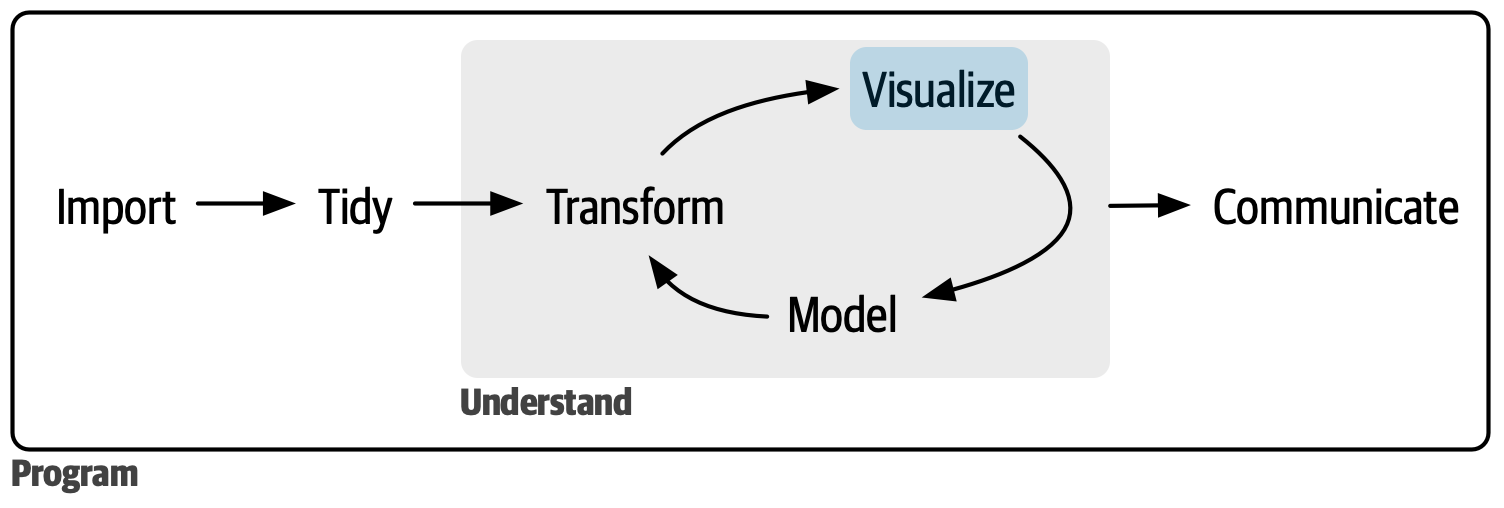
\includegraphics[width=5.57in,height=\textheight]{diagrams/data-science/visualize.png}

}

\caption{\label{fig-ds-visualize}Data visualization is often the first
step in data exploration.}

\end{figure}%

每一章都会介绍创建数据可视化的一个或多个方面。

\begin{itemize}
\tightlist
\item
  在 章节~\ref{sec-layers} 部分,学习图形的分层语法;
\item
  在 章节~\ref{sec-exploratory-data-analysis}
  部分,把可视化与你的好奇心和怀疑精神结合起来,针对数据提出并回答有趣的问题;
\item
  最后, 在 章节~\ref{sec-communication}
  部分,学习如何将探索性图形提升为解释性图形,这些图形有助于新手尽快理解你的分析结果。
\end{itemize}

这三章带你进入可视化的世界,但还有更多要学习的内容。学
习更多知识的绝佳选择是ggplot2:\href{https://ggplot2-book.org/}{\emph{ggplot2:
Elegant graphics for data analysis}}.。这
本书深入探讨了底层理论,并提供了许多如何将各个部分组合起来解决实际问题的示例。另
一个很好的资源是ggplot2扩展库\href{https://exts.ggplot2.tidyverse.org/gallery/\%E3\%80\%82\%E8\%BF\%99\%E4\%B8\%AA\%E7\%BD\%91\%E7\%AB\%99\%E5\%88\%97\%E5\%87\%BA\%E4\%BA\%86\%E8\%AE\%B8\%E5\%A4\%9A\%E7\%94\%A8\%E6\%96\%B0\%E7\%9A\%84\%E5\%87\%A0\%E4\%BD\%95\%E5\%9B\%BE\%E5\%BD\%A2\%E5\%92\%8C\%E6\%AF\%94\%E4\%BE\%8B\%E5\%B0\%BA\%E6\%89\%A9\%E5\%B1\%95ggplot2\%E7\%9A\%84\%E5\%8C\%85\%E3\%80\%82\%E5\%A6\%82\%E6\%9E\%9C\%E4\%BD\%A0\%E8\%AF\%95\%E5\%9B\%BE\%E7\%94\%A8ggplot2\%E5\%81\%9A\%E4\%B8\%80\%E4\%BA\%9B\%E7\%9C\%8B\%E4\%BC\%BC\%E5\%9B\%B0\%E9\%9A\%BE\%E7\%9A\%84\%E4\%BA\%8B\%E6\%83\%85\%EF\%BC\%8C\%E8\%BF\%99\%E6\%98\%AF\%E4\%B8\%80\%E4\%B8\%AA\%E5\%BE\%88\%E5\%A5\%BD\%E7\%9A\%84\%E8\%B5\%B7\%E7\%82\%B9\%E3\%80\%82}{https://exts.ggplot2.tidyverse.org/gallery/}。这
个网站列出了许多用新的geoms和scales扩展ggplot2的包。如
果你试图用ggplot2做一些看似困难的事情,这是一个很好的出发点。

\chapter{图层}\label{sec-layers}

\section{引言}\label{ux5f15ux8a00-4}

在 章节~\ref{sec-data-visualization} 中,
你学到的远不止如何制作散点图、条形图和箱线图。你
学习了利用\texttt{ggplot2}可以制作任何类型图形的基础知识。

在本章中你将在这个基础上进行扩展,学习图形的分层语法。首
先,我们将更深入地探讨美学映射、几何对象和切面。然
后,你将了解\texttt{ggplot2}在创建图形时背后进行的统计转换。这
些转换用于计算新的绘图值,例如条形图中的条形高度或箱线图的中位数。你
还将学习位置调整,这会修改几何对象在图表中的显示方式。最
后,我们将简要介绍坐标系。

我们不会涵盖这些图层中的每一个函数和选项,但我们将引导你了解\texttt{ggplot2}提供的最重要和最常用的功能,并向你介绍扩展\texttt{ggplot2}的包。

\subsection{必要条件}\label{ux5fc5ux8981ux6761ux4ef6-4}

本章重点介绍ggplot2。要
访问本章中使用的数据集、帮助页面和函数,请运行以下代码加载tidyverse:

\begin{Shaded}
\begin{Highlighting}[]
\FunctionTok{library}\NormalTok{(tidyverse)}
\end{Highlighting}
\end{Shaded}

\section{美学映射}\label{ux7f8eux5b66ux6620ux5c04}

\begin{quote}
``图片的最大价值在于它能够迫使我们注意到我们从未预期到的内容。''

--- John Tukey
\end{quote}

请记住,ggplot2 包附带的 \texttt{mpg}
数据框包含了关于38种不同汽车型号的234条观测数据。

\begin{Shaded}
\begin{Highlighting}[]
\NormalTok{mpg}
\CommentTok{\#\textgreater{} \# A tibble: 234 x 11}
\CommentTok{\#\textgreater{}   manufacturer model displ  year   cyl trans      drv     cty   hwy fl   }
\CommentTok{\#\textgreater{}   \textless{}chr\textgreater{}        \textless{}chr\textgreater{} \textless{}dbl\textgreater{} \textless{}int\textgreater{} \textless{}int\textgreater{} \textless{}chr\textgreater{}      \textless{}chr\textgreater{} \textless{}int\textgreater{} \textless{}int\textgreater{} \textless{}chr\textgreater{}}
\CommentTok{\#\textgreater{} 1 audi         a4      1.8  1999     4 auto(l5)   f        18    29 p    }
\CommentTok{\#\textgreater{} 2 audi         a4      1.8  1999     4 manual(m5) f        21    29 p    }
\CommentTok{\#\textgreater{} 3 audi         a4      2    2008     4 manual(m6) f        20    31 p    }
\CommentTok{\#\textgreater{} 4 audi         a4      2    2008     4 auto(av)   f        21    30 p    }
\CommentTok{\#\textgreater{} 5 audi         a4      2.8  1999     6 auto(l5)   f        16    26 p    }
\CommentTok{\#\textgreater{} 6 audi         a4      2.8  1999     6 manual(m5) f        18    26 p    }
\CommentTok{\#\textgreater{} \# i 228 more rows}
\CommentTok{\#\textgreater{} \# i 1 more variable: class \textless{}chr\textgreater{}}
\end{Highlighting}
\end{Shaded}

\texttt{mpg} 中的变量包括:

\begin{enumerate}
\def\labelenumi{\arabic{enumi}.}
\item
  \texttt{displ}: 汽车发动机的排量,单位为升。这 是一个数值型变量。
\item
  \texttt{hwy}:
  高速公路上汽车的燃油效率,以每加仑行驶的英里数(mpg)为单位。当
  两辆汽车行驶相同的距离时,燃油效率低的汽车比燃油效率高的汽车消耗更多的燃油。这
  是一个数值型变量。
\item
  \texttt{class}: 汽车的型号。这 是一个分类变量。
\end{enumerate}

让我们首先通过可视化不同车型类别(\texttt{class})的排量(\texttt{displ})和高速公路燃油效率(\texttt{hwy})之间的关系来开始。我
们可以使用散点图来实现这一点,其中数值变量映射到 \texttt{x} 和
\texttt{y}
美学上,而分类变量则映射到\texttt{color}或\texttt{shape}等美学上。

\begin{Shaded}
\begin{Highlighting}[]
\CommentTok{\# Left}
\FunctionTok{ggplot}\NormalTok{(mpg, }\FunctionTok{aes}\NormalTok{(}\AttributeTok{x =}\NormalTok{ displ, }\AttributeTok{y =}\NormalTok{ hwy, }\AttributeTok{color =}\NormalTok{ class)) }\SpecialCharTok{+}
  \FunctionTok{geom\_point}\NormalTok{()}

\CommentTok{\# Right}
\FunctionTok{ggplot}\NormalTok{(mpg, }\FunctionTok{aes}\NormalTok{(}\AttributeTok{x =}\NormalTok{ displ, }\AttributeTok{y =}\NormalTok{ hwy, }\AttributeTok{shape =}\NormalTok{ class)) }\SpecialCharTok{+}
  \FunctionTok{geom\_point}\NormalTok{()}
\CommentTok{\#\textgreater{} Warning: The shape palette can deal with a maximum of 6 discrete values because more}
\CommentTok{\#\textgreater{} than 6 becomes difficult to discriminate}
\CommentTok{\#\textgreater{} i you have requested 7 values. Consider specifying shapes manually if you}
\CommentTok{\#\textgreater{}   need that many have them.}
\CommentTok{\#\textgreater{} Warning: Removed 62 rows containing missing values or values outside the scale range}
\CommentTok{\#\textgreater{} (\textasciigrave{}geom\_point()\textasciigrave{}).}
\end{Highlighting}
\end{Shaded}

\begin{figure}

\begin{minipage}{0.50\linewidth}
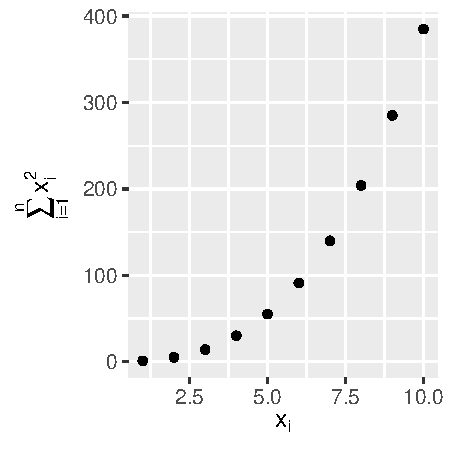
\includegraphics[width=12.5in,height=\textheight]{layers_files/figure-pdf/unnamed-chunk-4-1.pdf}\end{minipage}%
%
\begin{minipage}{0.50\linewidth}
\includegraphics[width=12.5in,height=\textheight]{layers_files/figure-pdf/unnamed-chunk-4-2.pdf}\end{minipage}%

\end{figure}%

当类别(\texttt{class})映射到形状(\texttt{shape})时,我们得到了两个警告:

\begin{quote}
1: 形状调色板最多只能处理 6 个离散值,因为超过 6
个值后就很难区分;但你有 7 个。如 果你必须使用它们,请考虑手动指定形状。

2: 删除了包含缺失值的 62 行(\texttt{geom\_point()})。
\end{quote}

由于 ggplot2
默认一次只会使用六个形状,因此当使用形状美学时,额外的组将不会被绘制。第
二个警告与此相关------数据集中有 62 辆 SUV,它们没有被绘制出来。

类似地,我们也可以将类别(\texttt{class})映射到大小(\texttt{size})或透明度(\texttt{alpha})美学上,它们分别控制点的大小和透明度。

\begin{Shaded}
\begin{Highlighting}[]
\CommentTok{\# Left}
\FunctionTok{ggplot}\NormalTok{(mpg, }\FunctionTok{aes}\NormalTok{(}\AttributeTok{x =}\NormalTok{ displ, }\AttributeTok{y =}\NormalTok{ hwy, }\AttributeTok{size =}\NormalTok{ class)) }\SpecialCharTok{+}
  \FunctionTok{geom\_point}\NormalTok{()}
\CommentTok{\#\textgreater{} Warning: Using size for a discrete variable is not advised.}

\CommentTok{\# Right}
\FunctionTok{ggplot}\NormalTok{(mpg, }\FunctionTok{aes}\NormalTok{(}\AttributeTok{x =}\NormalTok{ displ, }\AttributeTok{y =}\NormalTok{ hwy, }\AttributeTok{alpha =}\NormalTok{ class)) }\SpecialCharTok{+}
  \FunctionTok{geom\_point}\NormalTok{()}
\CommentTok{\#\textgreater{} Warning: Using alpha for a discrete variable is not advised.}
\end{Highlighting}
\end{Shaded}

\begin{figure}

\begin{minipage}{0.50\linewidth}
\includegraphics[width=12.5in,height=\textheight]{layers_files/figure-pdf/unnamed-chunk-5-1.pdf}\end{minipage}%
%
\begin{minipage}{0.50\linewidth}
\includegraphics[width=12.5in,height=\textheight]{layers_files/figure-pdf/unnamed-chunk-5-2.pdf}\end{minipage}%

\end{figure}%

这两种方法都会产生警告:

\begin{quote}
不建议将alpha用作离散变量。
\end{quote}

将一个无序的离散(分类)变量(如车型\texttt{class})映射到一个有序的美学属性(如大小\texttt{size}或透明度\texttt{alpha})通常不是明智之举,因为它暗含了一个实际上并不存在的排名。

一旦你映射了一个美学属性,ggplot2 就会处理其余部分。它
会选择一个合理的刻度来与这个美学属性一起使用,并构造一个图例来解释水平和值之间的映射关系。对
于 x 和 y 美学属性,ggplot2
不会创建图例,但会创建一个带有刻度线和标签的坐标轴线。坐
标轴线提供了与图例相同的信息;它解释了位置和值之间的映射关系。

你也可以通过几何对象函数的参数(在 \texttt{aes()}
之外)来手动设置你的几何对象的视觉属性,而不是依赖变量映射来确定外观。例
如,我们可以让我们的图形中的所有点都呈现蓝色:

\begin{Shaded}
\begin{Highlighting}[]
\FunctionTok{ggplot}\NormalTok{(mpg, }\FunctionTok{aes}\NormalTok{(}\AttributeTok{x =}\NormalTok{ displ, }\AttributeTok{y =}\NormalTok{ hwy)) }\SpecialCharTok{+} 
  \FunctionTok{geom\_point}\NormalTok{(}\AttributeTok{color =} \StringTok{"blue"}\NormalTok{)}
\end{Highlighting}
\end{Shaded}

\includegraphics[width=18.75in,height=\textheight]{layers_files/figure-pdf/unnamed-chunk-6-1.pdf}

在这里颜色并不传达关于变量的信息,而只是改变图的外观。你
需要选择一个对该美学属性有意义的值:

\begin{itemize}
\tightlist
\item
  颜色的名称作为字符串, 例如 \texttt{color\ =\ "blue"}
\item
  点的大小以毫米为单位,例如 \texttt{size\ =\ 1}
\item
  点的形状作为一个数字,例如 \texttt{shape\ =\ 1}, 如图
  图~\ref{fig-shapes} 所示。
\end{itemize}

\begin{figure}

\centering{

\includegraphics[width=18.75in,height=\textheight]{layers_files/figure-pdf/fig-shapes-1.pdf}

}

\caption{\label{fig-shapes}R has 25 built-in shapes that are identified
by numbers. There are some seeming duplicates: for example, 0, 15, and
22 are all squares. The difference comes from the interaction of the
\texttt{color} and \texttt{fill} aesthetics. The hollow shapes (0--14)
have a border determined by \texttt{color}; the solid shapes (15--20)
are filled with \texttt{color}; the filled shapes (21--24) have a border
of \texttt{color} and are filled with \texttt{fill}. Shapes are arranged
to keep similar shapes next to each other.}

\end{figure}%

到目前为止,我们讨论了在使用点几何对象(point
geom)创建散点图时可以映射或设置的美学属性。你
可以在\url{https://ggplot2.tidyverse.org/articles/ggplot2-specs.html}
的美学规范文档中了解更多关于所有可能的美学映射的信息。

你可以在一个图中使用的具体美学属性取决于你用来表示数据的几何对象(geom)。在
下一节中,我们将更深入地探讨几何对象。

\subsection{练习}\label{ux7ec3ux4e60-12}

\begin{enumerate}
\def\labelenumi{\arabic{enumi}.}
\item
  创建一个\texttt{hwy}和\texttt{displ}的散点图,其中的点是粉红色填充的三角形。
\item
  以下代码为什么没有生成带有蓝色点的图:

\begin{Shaded}
\begin{Highlighting}[]
\FunctionTok{ggplot}\NormalTok{(mpg) }\SpecialCharTok{+} 
  \FunctionTok{geom\_point}\NormalTok{(}\FunctionTok{aes}\NormalTok{(}\AttributeTok{x =}\NormalTok{ displ, }\AttributeTok{y =}\NormalTok{ hwy, }\AttributeTok{color =} \StringTok{"blue"}\NormalTok{))}
\end{Highlighting}
\end{Shaded}
\item
  描边美学(stroke aesthetic)是做什么用的?它 与哪些形状一起工作?(
  提示:使用 \texttt{?geom\_point})
\item
  如果你将美学映射到变量名之外的其他东西,比如
  \texttt{aes(color\ =\ displ\ \textless{}\ 5)},会发生什么?注
  意,你还需要指定 x 和 y。
\end{enumerate}

\section{几何对象}\label{sec-geometric-objects}

下面两张图有什么相似之处?

\begin{figure}

\begin{minipage}{0.50\linewidth}
\includegraphics[width=9.375in,height=\textheight]{layers_files/figure-pdf/unnamed-chunk-9-1.pdf}\end{minipage}%
%
\begin{minipage}{0.50\linewidth}
\includegraphics[width=9.375in,height=\textheight]{layers_files/figure-pdf/unnamed-chunk-9-2.pdf}\end{minipage}%

\end{figure}%

两张图包含相同的x变量和y变量,并且都描述了相同的数据。但
是,这两张图并不完全相同。每
张图都使用不同的几何对象(geom)来表示数据。左
侧的图使用了点几何对象(point
geom),而右侧的图表使用了平滑几何对象(smooth
geom),即用平滑线拟合到数据上。

要在你的图中更改几何对象(geom),请更改你添加到\texttt{ggplot()}函数中的几何对象函数。例
如,要绘制上述图可以使用以下代码:

\begin{Shaded}
\begin{Highlighting}[]
\CommentTok{\# Left}
\FunctionTok{ggplot}\NormalTok{(mpg, }\FunctionTok{aes}\NormalTok{(}\AttributeTok{x =}\NormalTok{ displ, }\AttributeTok{y =}\NormalTok{ hwy)) }\SpecialCharTok{+} 
  \FunctionTok{geom\_point}\NormalTok{()}

\CommentTok{\# Right}
\FunctionTok{ggplot}\NormalTok{(mpg, }\FunctionTok{aes}\NormalTok{(}\AttributeTok{x =}\NormalTok{ displ, }\AttributeTok{y =}\NormalTok{ hwy)) }\SpecialCharTok{+} 
  \FunctionTok{geom\_smooth}\NormalTok{()}
\CommentTok{\#\textgreater{} \textasciigrave{}geom\_smooth()\textasciigrave{} using method = \textquotesingle{}loess\textquotesingle{} and formula = \textquotesingle{}y \textasciitilde{} x\textquotesingle{}}
\end{Highlighting}
\end{Shaded}

在ggplot2中,每个geom函数都接受一个映射参数,这个参数可以在geom图层中本地定义,也可以在\texttt{ggplot()}图层中全局定义。然
而,并不是每个美学属性(aesthetic)都适用于每个geom。你
可以设置点的形状,但你不能设置线的``形状''。如
果你尝试这样做,ggplot2会静默地忽略该美学映射。另
一方面,你可以设置线的线型。\texttt{g}
\texttt{eom\_smooth()}会根据你映射到线型变量的不同值,绘制具有不同线型的平滑线。

\begin{Shaded}
\begin{Highlighting}[]
\CommentTok{\# Left}
\FunctionTok{ggplot}\NormalTok{(mpg, }\FunctionTok{aes}\NormalTok{(}\AttributeTok{x =}\NormalTok{ displ, }\AttributeTok{y =}\NormalTok{ hwy, }\AttributeTok{shape =}\NormalTok{ drv)) }\SpecialCharTok{+} 
  \FunctionTok{geom\_smooth}\NormalTok{()}

\CommentTok{\# Right}
\FunctionTok{ggplot}\NormalTok{(mpg, }\FunctionTok{aes}\NormalTok{(}\AttributeTok{x =}\NormalTok{ displ, }\AttributeTok{y =}\NormalTok{ hwy, }\AttributeTok{linetype =}\NormalTok{ drv)) }\SpecialCharTok{+} 
  \FunctionTok{geom\_smooth}\NormalTok{()}
\end{Highlighting}
\end{Shaded}

\begin{figure}

\begin{minipage}{0.50\linewidth}
\includegraphics[width=9.375in,height=\textheight]{layers_files/figure-pdf/unnamed-chunk-11-1.pdf}\end{minipage}%
%
\begin{minipage}{0.50\linewidth}
\includegraphics[width=9.375in,height=\textheight]{layers_files/figure-pdf/unnamed-chunk-11-2.pdf}\end{minipage}%

\end{figure}%

在这里,\texttt{geom\_smooth()}根据汽车的\texttt{drv}值(描述了汽车的驱动方式)将汽车数据分成三条线。一
条线描述了所有值为4的点,一条线描述了所有值为\texttt{f}的点,还有一条线描述了所有值为\texttt{r}的点。在
这里,4代表四轮驱动,\texttt{f}代表前轮驱动,\texttt{r}代表后轮驱动。

如果这听起来有些奇怪,我们可以通过将这三条线叠加在原始数据上,并根据\texttt{drv}的值给所有内容上色,来使其更加清晰。

\begin{Shaded}
\begin{Highlighting}[]
\FunctionTok{ggplot}\NormalTok{(mpg, }\FunctionTok{aes}\NormalTok{(}\AttributeTok{x =}\NormalTok{ displ, }\AttributeTok{y =}\NormalTok{ hwy, }\AttributeTok{color =}\NormalTok{ drv)) }\SpecialCharTok{+} 
  \FunctionTok{geom\_point}\NormalTok{() }\SpecialCharTok{+}
  \FunctionTok{geom\_smooth}\NormalTok{(}\FunctionTok{aes}\NormalTok{(}\AttributeTok{linetype =}\NormalTok{ drv))}
\end{Highlighting}
\end{Shaded}

\includegraphics[width=18.75in,height=\textheight]{layers_files/figure-pdf/unnamed-chunk-12-1.pdf}

请注意,这个图在同一个图形中包含了两个几何对象(geoms)。

许多几何对象(如\texttt{geom\_smooth()})使用单个几何对象来显示多行数据。对
于这些几何对象,你可以将组(\texttt{group})美学属性设置为分类变量来绘制多个对象。g
gplot2会为分组变量的每个值绘制一个独立的对象。在
实践中,当你将美学属性映射到离散变量时(如线型示例),ggplot2会自动为这些几何对象分组数据。依
赖这个特性是很方便的,因为组(\texttt{group})美学属性本身不会给几何对象添加图例或区分特征。

\begin{Shaded}
\begin{Highlighting}[]
\CommentTok{\# Left}
\FunctionTok{ggplot}\NormalTok{(mpg, }\FunctionTok{aes}\NormalTok{(}\AttributeTok{x =}\NormalTok{ displ, }\AttributeTok{y =}\NormalTok{ hwy)) }\SpecialCharTok{+}
  \FunctionTok{geom\_smooth}\NormalTok{()}

\CommentTok{\# Middle}
\FunctionTok{ggplot}\NormalTok{(mpg, }\FunctionTok{aes}\NormalTok{(}\AttributeTok{x =}\NormalTok{ displ, }\AttributeTok{y =}\NormalTok{ hwy)) }\SpecialCharTok{+}
  \FunctionTok{geom\_smooth}\NormalTok{(}\FunctionTok{aes}\NormalTok{(}\AttributeTok{group =}\NormalTok{ drv))}

\CommentTok{\# Right}
\FunctionTok{ggplot}\NormalTok{(mpg, }\FunctionTok{aes}\NormalTok{(}\AttributeTok{x =}\NormalTok{ displ, }\AttributeTok{y =}\NormalTok{ hwy)) }\SpecialCharTok{+}
  \FunctionTok{geom\_smooth}\NormalTok{(}\FunctionTok{aes}\NormalTok{(}\AttributeTok{color =}\NormalTok{ drv), }\AttributeTok{show.legend =} \ConstantTok{FALSE}\NormalTok{)}
\end{Highlighting}
\end{Shaded}

\begin{figure}

\begin{minipage}{0.33\linewidth}
\includegraphics[width=9.375in,height=\textheight]{layers_files/figure-pdf/unnamed-chunk-13-1.pdf}\end{minipage}%
%
\begin{minipage}{0.33\linewidth}
\includegraphics[width=9.375in,height=\textheight]{layers_files/figure-pdf/unnamed-chunk-13-2.pdf}\end{minipage}%
%
\begin{minipage}{0.33\linewidth}
\includegraphics[width=9.375in,height=\textheight]{layers_files/figure-pdf/unnamed-chunk-13-3.pdf}\end{minipage}%

\end{figure}%

如果你在geom函数中放置映射,ggplot2会将这些映射视为该图层的本地映射。它
将使用这些映射来扩展或覆盖该图层的全局映射。这
使得在不同的图层中显示不同的美学属性成为可能。

\begin{Shaded}
\begin{Highlighting}[]
\FunctionTok{ggplot}\NormalTok{(mpg, }\FunctionTok{aes}\NormalTok{(}\AttributeTok{x =}\NormalTok{ displ, }\AttributeTok{y =}\NormalTok{ hwy)) }\SpecialCharTok{+} 
  \FunctionTok{geom\_point}\NormalTok{(}\FunctionTok{aes}\NormalTok{(}\AttributeTok{color =}\NormalTok{ class)) }\SpecialCharTok{+} 
  \FunctionTok{geom\_smooth}\NormalTok{()}
\end{Highlighting}
\end{Shaded}

\includegraphics[width=18.75in,height=\textheight]{layers_files/figure-pdf/unnamed-chunk-14-1.pdf}

你可以使用相同的思路来为每一层指定不同的数据。在
这里,我们使用红色的点和空心的圆圈来突出显示两座车。\texttt{g}
\texttt{eom\_point()}中的局部数据参数(local data
argument)仅针对那一层覆盖了\texttt{ggplot()}中的全局数据参数(global
data argument)。

\begin{Shaded}
\begin{Highlighting}[]
\FunctionTok{ggplot}\NormalTok{(mpg, }\FunctionTok{aes}\NormalTok{(}\AttributeTok{x =}\NormalTok{ displ, }\AttributeTok{y =}\NormalTok{ hwy)) }\SpecialCharTok{+} 
  \FunctionTok{geom\_point}\NormalTok{() }\SpecialCharTok{+} 
  \FunctionTok{geom\_point}\NormalTok{(}
    \AttributeTok{data =}\NormalTok{ mpg }\SpecialCharTok{|\textgreater{}} \FunctionTok{filter}\NormalTok{(class }\SpecialCharTok{==} \StringTok{"2seater"}\NormalTok{), }
    \AttributeTok{color =} \StringTok{"red"}
\NormalTok{  ) }\SpecialCharTok{+}
  \FunctionTok{geom\_point}\NormalTok{(}
    \AttributeTok{data =}\NormalTok{ mpg }\SpecialCharTok{|\textgreater{}} \FunctionTok{filter}\NormalTok{(class }\SpecialCharTok{==} \StringTok{"2seater"}\NormalTok{), }
    \AttributeTok{shape =} \StringTok{"circle open"}\NormalTok{, }\AttributeTok{size =} \DecValTok{3}\NormalTok{, }\AttributeTok{color =} \StringTok{"red"}
\NormalTok{  )}
\end{Highlighting}
\end{Shaded}

\includegraphics[width=18.75in,height=\textheight]{layers_files/figure-pdf/unnamed-chunk-15-1.pdf}

几何对象(\texttt{geoms})是\texttt{ggplot2}的基本构建模块。你
可以通过改变图形的\texttt{geom}来完全改变其外观,而不同的\texttt{geoms}可以揭示数据的不同特征。例
如下面的直方图和密度图揭示了高速公路里程的分布是双峰的且向右偏斜,而箱线图则揭示了两个潜在的异常值。

\begin{Shaded}
\begin{Highlighting}[]
\CommentTok{\# Left}
\FunctionTok{ggplot}\NormalTok{(mpg, }\FunctionTok{aes}\NormalTok{(}\AttributeTok{x =}\NormalTok{ hwy)) }\SpecialCharTok{+}
  \FunctionTok{geom\_histogram}\NormalTok{(}\AttributeTok{binwidth =} \DecValTok{2}\NormalTok{)}

\CommentTok{\# Middle}
\FunctionTok{ggplot}\NormalTok{(mpg, }\FunctionTok{aes}\NormalTok{(}\AttributeTok{x =}\NormalTok{ hwy)) }\SpecialCharTok{+}
  \FunctionTok{geom\_density}\NormalTok{()}

\CommentTok{\# Right}
\FunctionTok{ggplot}\NormalTok{(mpg, }\FunctionTok{aes}\NormalTok{(}\AttributeTok{x =}\NormalTok{ hwy)) }\SpecialCharTok{+}
  \FunctionTok{geom\_boxplot}\NormalTok{()}
\end{Highlighting}
\end{Shaded}

\begin{figure}

\begin{minipage}{0.33\linewidth}
\includegraphics[width=9.375in,height=\textheight]{layers_files/figure-pdf/unnamed-chunk-16-1.pdf}\end{minipage}%
%
\begin{minipage}{0.33\linewidth}
\includegraphics[width=9.375in,height=\textheight]{layers_files/figure-pdf/unnamed-chunk-16-2.pdf}\end{minipage}%
%
\begin{minipage}{0.33\linewidth}
\includegraphics[width=9.375in,height=\textheight]{layers_files/figure-pdf/unnamed-chunk-16-3.pdf}\end{minipage}%

\end{figure}%

ggplot2提供了超过 40
个\texttt{geoms},但这并不覆盖所有可能创建的图形。如
果你需要一个不同的\texttt{geom},我们建议先查看扩展包,看看是否有人已经实现了它(可以在\url{https://exts.ggplot2.tidyverse.org/gallery/}找到一个示例)。例
如,\texttt{ggridges}包(\href{https://wilkelab.org/ggridges/}{https://wilkelab.org/ggridges})对于制作山脊线图(ridgeline
plots)很有用,这种图可以用于可视化数值变量在不同类别变量水平下的密度。在
下面的图形中,我们不仅使用了一个新的\texttt{geom}(\texttt{geom\_density\_ridges()}),而且我们还将相同的变量映射到多个美学属性(\texttt{drv}到\texttt{y}、\texttt{fill}和\texttt{color}),并设置了一个美学属性(\texttt{alpha\ =\ 0.5})以使密度曲线透明。

\begin{Shaded}
\begin{Highlighting}[]
\FunctionTok{library}\NormalTok{(ggridges)}

\FunctionTok{ggplot}\NormalTok{(mpg, }\FunctionTok{aes}\NormalTok{(}\AttributeTok{x =}\NormalTok{ hwy, }\AttributeTok{y =}\NormalTok{ drv, }\AttributeTok{fill =}\NormalTok{ drv, }\AttributeTok{color =}\NormalTok{ drv)) }\SpecialCharTok{+}
  \FunctionTok{geom\_density\_ridges}\NormalTok{(}\AttributeTok{alpha =} \FloatTok{0.5}\NormalTok{, }\AttributeTok{show.legend =} \ConstantTok{FALSE}\NormalTok{)}
\CommentTok{\#\textgreater{} Picking joint bandwidth of 1.28}
\end{Highlighting}
\end{Shaded}

\includegraphics[width=18.75in,height=\textheight]{layers_files/figure-pdf/unnamed-chunk-17-1.pdf}

要了解\texttt{ggplot2}提供的所有\texttt{geoms}的全面概述以及包中的所有函数,最好的地方是参考\url{https://ggplot2.tidyverse.org/reference}。要
深入了解任何单一的\texttt{geom},请使用帮助函数(例如
\texttt{?geom\_smooth})。

\subsection{练习}\label{ux7ec3ux4e60-13}

\begin{enumerate}
\def\labelenumi{\arabic{enumi}.}
\item
  你会使用哪种\texttt{geom}来绘制折线图?箱 线图?直 方图?面 积图?
\item
  在本章的前面部分,我们使用了\texttt{show.legend}而没有解释它:

\begin{Shaded}
\begin{Highlighting}[]
\FunctionTok{ggplot}\NormalTok{(mpg, }\FunctionTok{aes}\NormalTok{(}\AttributeTok{x =}\NormalTok{ displ, }\AttributeTok{y =}\NormalTok{ hwy)) }\SpecialCharTok{+}
  \FunctionTok{geom\_smooth}\NormalTok{(}\FunctionTok{aes}\NormalTok{(}\AttributeTok{color =}\NormalTok{ drv), }\AttributeTok{show.legend =} \ConstantTok{FALSE}\NormalTok{)}
\end{Highlighting}
\end{Shaded}

  \texttt{show.legend\ =\ FALSE}在这里的作用是什么?如
  果你把它去掉会怎么样?你 觉得我们之前为什么用它?
\item
  \texttt{geom\_smooth()} 的参数\texttt{se}起什么作用?
\item
  重新创建生成以下图形所需的R代码。
  请注意,图中用到的分类变量的都是\texttt{drv}。

  \begin{figure}

  \begin{minipage}{0.50\linewidth}
  \includegraphics[width=9.375in,height=\textheight]{layers_files/figure-pdf/unnamed-chunk-19-1.pdf}\end{minipage}%
  %
  \begin{minipage}{0.50\linewidth}
  \includegraphics[width=9.375in,height=\textheight]{layers_files/figure-pdf/unnamed-chunk-19-2.pdf}\end{minipage}%
  \newline
  \begin{minipage}{0.50\linewidth}
  \includegraphics[width=9.375in,height=\textheight]{layers_files/figure-pdf/unnamed-chunk-19-3.pdf}\end{minipage}%
  %
  \begin{minipage}{0.50\linewidth}
  \includegraphics[width=9.375in,height=\textheight]{layers_files/figure-pdf/unnamed-chunk-19-4.pdf}\end{minipage}%
  \newline
  \begin{minipage}{0.50\linewidth}
  \includegraphics[width=9.375in,height=\textheight]{layers_files/figure-pdf/unnamed-chunk-19-5.pdf}\end{minipage}%
  %
  \begin{minipage}{0.50\linewidth}
  \includegraphics[width=9.375in,height=\textheight]{layers_files/figure-pdf/unnamed-chunk-19-6.pdf}\end{minipage}%

  \end{figure}%
\end{enumerate}

\section{分面}\label{ux5206ux9762}

在 章节~\ref{sec-data-visualization}
,你学习了使用\texttt{facet\_wrap()}进行分面,该方法可以将一个图形分割成子图,每个子图都基于一个分类变量显示数据的一个子集。

\begin{Shaded}
\begin{Highlighting}[]
\FunctionTok{ggplot}\NormalTok{(mpg, }\FunctionTok{aes}\NormalTok{(}\AttributeTok{x =}\NormalTok{ displ, }\AttributeTok{y =}\NormalTok{ hwy)) }\SpecialCharTok{+} 
  \FunctionTok{geom\_point}\NormalTok{() }\SpecialCharTok{+} 
  \FunctionTok{facet\_wrap}\NormalTok{(}\SpecialCharTok{\textasciitilde{}}\NormalTok{cyl)}
\end{Highlighting}
\end{Shaded}

\includegraphics[width=18.75in,height=\textheight]{layers_files/figure-pdf/unnamed-chunk-20-1.pdf}

要使用两个变量的组合来对你的图形进行分面,你需要从\texttt{facet\_wrap()}切换到\texttt{facet\_grid()}。\texttt{f}
\texttt{acet\_grid()}的第一个参数也是一个公式,但现在它是一个双面公式:\texttt{rows\ \textasciitilde{}\ cols}。

\begin{Shaded}
\begin{Highlighting}[]
\FunctionTok{ggplot}\NormalTok{(mpg, }\FunctionTok{aes}\NormalTok{(}\AttributeTok{x =}\NormalTok{ displ, }\AttributeTok{y =}\NormalTok{ hwy)) }\SpecialCharTok{+} 
  \FunctionTok{geom\_point}\NormalTok{() }\SpecialCharTok{+} 
  \FunctionTok{facet\_grid}\NormalTok{(drv }\SpecialCharTok{\textasciitilde{}}\NormalTok{ cyl)}
\end{Highlighting}
\end{Shaded}

\includegraphics[width=18.75in,height=\textheight]{layers_files/figure-pdf/unnamed-chunk-21-1.pdf}

默认情况下,每个分面共享相同的x轴和y轴的刻度和范围。当
你想跨分面比较数据时,这很有用,但当你希望更好地可视化每个分面内的关系时,这可能会有所限制。将
分面函数中的\texttt{scales}参数设置为\texttt{"free"}将允许行和列之间使用不同的轴刻度,``\texttt{free\_x}''将允许行之间使用不同的刻度,``\texttt{free\_y}''将允许列之间使用不同的刻度。

\begin{Shaded}
\begin{Highlighting}[]
\FunctionTok{ggplot}\NormalTok{(mpg, }\FunctionTok{aes}\NormalTok{(}\AttributeTok{x =}\NormalTok{ displ, }\AttributeTok{y =}\NormalTok{ hwy)) }\SpecialCharTok{+} 
  \FunctionTok{geom\_point}\NormalTok{() }\SpecialCharTok{+} 
  \FunctionTok{facet\_grid}\NormalTok{(drv }\SpecialCharTok{\textasciitilde{}}\NormalTok{ cyl, }\AttributeTok{scales =} \StringTok{"free\_y"}\NormalTok{)}
\end{Highlighting}
\end{Shaded}

\includegraphics[width=18.75in,height=\textheight]{layers_files/figure-pdf/unnamed-chunk-22-1.pdf}

\subsection{练习}\label{ux7ec3ux4e60-14}

\begin{enumerate}
\def\labelenumi{\arabic{enumi}.}
\item
  如果你对一个连续变量进行分面会发生什么?
\item
  上面的图中使用\texttt{facet\_grid(drv\ \textasciitilde{}\ cyl)}生成的空单元格是什么意思?运
  行以下代码,它们与生成的图有什么关系?

\begin{Shaded}
\begin{Highlighting}[]
\FunctionTok{ggplot}\NormalTok{(mpg) }\SpecialCharTok{+} 
  \FunctionTok{geom\_point}\NormalTok{(}\FunctionTok{aes}\NormalTok{(}\AttributeTok{x =}\NormalTok{ drv, }\AttributeTok{y =}\NormalTok{ cyl))}
\end{Highlighting}
\end{Shaded}
\item
  以下代码生成了什么样的图形?\texttt{.} 在这里代表什么?

\begin{Shaded}
\begin{Highlighting}[]
\FunctionTok{ggplot}\NormalTok{(mpg) }\SpecialCharTok{+} 
  \FunctionTok{geom\_point}\NormalTok{(}\FunctionTok{aes}\NormalTok{(}\AttributeTok{x =}\NormalTok{ displ, }\AttributeTok{y =}\NormalTok{ hwy)) }\SpecialCharTok{+}
  \FunctionTok{facet\_grid}\NormalTok{(drv }\SpecialCharTok{\textasciitilde{}}\NormalTok{ .)}

\FunctionTok{ggplot}\NormalTok{(mpg) }\SpecialCharTok{+} 
  \FunctionTok{geom\_point}\NormalTok{(}\FunctionTok{aes}\NormalTok{(}\AttributeTok{x =}\NormalTok{ displ, }\AttributeTok{y =}\NormalTok{ hwy)) }\SpecialCharTok{+}
  \FunctionTok{facet\_grid}\NormalTok{(. }\SpecialCharTok{\textasciitilde{}}\NormalTok{ cyl)}
\end{Highlighting}
\end{Shaded}
\item
  查看本节中的第一个分面图:

\begin{Shaded}
\begin{Highlighting}[]
\FunctionTok{ggplot}\NormalTok{(mpg) }\SpecialCharTok{+} 
  \FunctionTok{geom\_point}\NormalTok{(}\FunctionTok{aes}\NormalTok{(}\AttributeTok{x =}\NormalTok{ displ, }\AttributeTok{y =}\NormalTok{ hwy)) }\SpecialCharTok{+} 
  \FunctionTok{facet\_wrap}\NormalTok{(}\SpecialCharTok{\textasciitilde{}}\NormalTok{ class, }\AttributeTok{nrow =} \DecValTok{2}\NormalTok{)}
\end{Highlighting}
\end{Shaded}

  使用分面(faceting)而不是颜色美学(color aesthetic)的优势是什么?劣
  势是什么?如 果你有一个更大的数据集,这种平衡可能会如何改变?
\item
  阅读\texttt{?facet\_wrap}的帮助文档,\texttt{nrow}是做什么的?\texttt{n}
  \texttt{col}呢?还 有哪些选项控制单个面板的布局?为
  什么\texttt{facet\_grid()}没有\texttt{nrow}和\texttt{ncol}参数?
\item
  下面的哪个图使得比较不同驱动方式的汽车的发动机排量(\texttt{displ})更容易?

\begin{Shaded}
\begin{Highlighting}[]
\FunctionTok{ggplot}\NormalTok{(mpg, }\FunctionTok{aes}\NormalTok{(}\AttributeTok{x =}\NormalTok{ displ)) }\SpecialCharTok{+} 
  \FunctionTok{geom\_histogram}\NormalTok{() }\SpecialCharTok{+} 
  \FunctionTok{facet\_grid}\NormalTok{(drv }\SpecialCharTok{\textasciitilde{}}\NormalTok{ .)}

\FunctionTok{ggplot}\NormalTok{(mpg, }\FunctionTok{aes}\NormalTok{(}\AttributeTok{x =}\NormalTok{ displ)) }\SpecialCharTok{+} 
  \FunctionTok{geom\_histogram}\NormalTok{() }\SpecialCharTok{+}
  \FunctionTok{facet\_grid}\NormalTok{(. }\SpecialCharTok{\textasciitilde{}}\NormalTok{ drv)}
\end{Highlighting}
\end{Shaded}
\item
  使用\texttt{facet\_wrap()}重新创建以下图形。这
  时分面标签的位置如何变化?

\begin{Shaded}
\begin{Highlighting}[]
\FunctionTok{ggplot}\NormalTok{(mpg) }\SpecialCharTok{+} 
  \FunctionTok{geom\_point}\NormalTok{(}\FunctionTok{aes}\NormalTok{(}\AttributeTok{x =}\NormalTok{ displ, }\AttributeTok{y =}\NormalTok{ hwy)) }\SpecialCharTok{+}
  \FunctionTok{facet\_grid}\NormalTok{(drv }\SpecialCharTok{\textasciitilde{}}\NormalTok{ .)}
\end{Highlighting}
\end{Shaded}
\end{enumerate}

\section{统计变换}\label{ux7edfux8ba1ux53d8ux6362}

下面是一个用\texttt{geom\_bar()}或\texttt{geom\_col()}绘制的基本条形图,图形显示了\texttt{diamonds}数据集中按\texttt{cut}分组的钻石总数。\texttt{d}
\texttt{iamonds}数据集位于\texttt{ggplot2}包中,包含约 54,000
颗钻石的信息,包括每颗钻石的价格(\texttt{price})、重量(\texttt{carat})、颜色(\texttt{color})、净度(\texttt{clarity})和切割方式(\texttt{cut}
)。图 形显示,高质量切割的钻石比低质量切割的钻石更多。

\begin{Shaded}
\begin{Highlighting}[]
\FunctionTok{ggplot}\NormalTok{(diamonds, }\FunctionTok{aes}\NormalTok{(}\AttributeTok{x =}\NormalTok{ cut)) }\SpecialCharTok{+} 
  \FunctionTok{geom\_bar}\NormalTok{()}
\end{Highlighting}
\end{Shaded}

\includegraphics[width=18.75in,height=\textheight]{layers_files/figure-pdf/unnamed-chunk-28-1.pdf}

在 x 轴上图形显示了来自 \texttt{diamonds} 数据集的变量 \texttt{cut}。在
y 轴上显示了 count,但 count 并不是 \texttt{diamonds} 数据集中的变量!c
ount 是从哪里来的?许 多图形,如散点图会绘制数据集的原始值。而
其他图形,如条形图则会计算新的值来绘制:

\begin{itemize}
\tightlist
\item
  条形图、直方图和频数多边形会将数据进行分箱,然后绘制每个分箱中的点数(即分箱计数)。
\item
  平滑器(smoothers)会对您的数据拟合一个模型,然后绘制该模型的预测值。
\item
  箱线图会计算分布的五数汇总(five-number
  summary),然后以特殊格式的箱子显示该汇总。
\end{itemize}

用于计算图形新值的算法被称为 \textbf{stat},是 statistical
transformation(统计变换)的缩写。@ fig-vis-stat-bar 展示了
\texttt{geom\_bar()} 是如何工作的。

\begin{figure}

\centering{

\includegraphics[width=1\textwidth,height=\textheight]{images/visualization-stat-bar.png}

}

\caption{\label{fig-vis-stat-bar}When creating a bar chart we first
start with the raw data, then aggregate it to count the number of
observations in each bar, and finally map those computed variables to
plot aesthetics.}

\end{figure}%

你可以通过检查\texttt{stat}参数的默认值来了解一个\texttt{geom}使用的是哪种统计变换。例
如\texttt{?geom\_bar}显示\texttt{stat}的默认值是''count'',这意味着\texttt{geom\_bar()}使用的是\texttt{stat\_count()}。\texttt{s}
\texttt{tat\_count()}的文档与\texttt{geom\_bar()}在同一页面。如
果你向下滚动,名为``Computed
variables''的部分说明它计算了两个新变量:\texttt{count}和\texttt{prop}。

每个\texttt{geom}都有一个默认的统计变换;每个统计变换也有一个默认的\texttt{geom}。这
意味着你通常可以使用\texttt{geoms}而不用担心底层的统计变换。然
而,在三种情况下你可能需要指明使用何种统计变换:

\begin{enumerate}
\def\labelenumi{\arabic{enumi}.}
\item
  你可能想要覆盖默认的统计变换。在
  下面的代码中,我们将\texttt{geom\_bar()}的统计变换从默认的count更改为identity。这
  样我们就可以将条形的高度映射到 y 变量的原始值。

\begin{Shaded}
\begin{Highlighting}[]
\NormalTok{diamonds }\SpecialCharTok{|\textgreater{}}
  \FunctionTok{count}\NormalTok{(cut) }\SpecialCharTok{|\textgreater{}}
  \FunctionTok{ggplot}\NormalTok{(}\FunctionTok{aes}\NormalTok{(}\AttributeTok{x =}\NormalTok{ cut, }\AttributeTok{y =}\NormalTok{ n)) }\SpecialCharTok{+}
  \FunctionTok{geom\_bar}\NormalTok{(}\AttributeTok{stat =} \StringTok{"identity"}\NormalTok{)}
\end{Highlighting}
\end{Shaded}

  \includegraphics[width=18.75in,height=\textheight]{layers_files/figure-pdf/unnamed-chunk-30-1.pdf}
\item
  你可能想要覆盖从变换后的变量到视觉属性的默认映射。例
  如,你可能想要显示一个比例条形图,而不是计数条形图:

\begin{Shaded}
\begin{Highlighting}[]
\FunctionTok{ggplot}\NormalTok{(diamonds, }\FunctionTok{aes}\NormalTok{(}\AttributeTok{x =}\NormalTok{ cut, }\AttributeTok{y =} \FunctionTok{after\_stat}\NormalTok{(prop), }\AttributeTok{group =} \DecValTok{1}\NormalTok{)) }\SpecialCharTok{+} 
  \FunctionTok{geom\_bar}\NormalTok{()}
\end{Highlighting}
\end{Shaded}

  \includegraphics[width=18.75in,height=\textheight]{layers_files/figure-pdf/unnamed-chunk-31-1.pdf}

  要找到可以由统计变换计算的可能的变量,请在\texttt{geom\_bar()}的帮助文档中寻找标题为``computed
  variables''的部分。
\item
  你可能希望在你的代码中更加关注统计变换。例
  如你可能使用\texttt{stat\_summary()},它对每个唯一的 x 值汇总 y
  值,以此来强调你正在计算的汇总统计量:

\begin{Shaded}
\begin{Highlighting}[]
\FunctionTok{ggplot}\NormalTok{(diamonds) }\SpecialCharTok{+} 
  \FunctionTok{stat\_summary}\NormalTok{(}
    \FunctionTok{aes}\NormalTok{(}\AttributeTok{x =}\NormalTok{ cut, }\AttributeTok{y =}\NormalTok{ depth),}
    \AttributeTok{fun.min =}\NormalTok{ min,}
    \AttributeTok{fun.max =}\NormalTok{ max,}
    \AttributeTok{fun =}\NormalTok{ median}
\NormalTok{  )}
\end{Highlighting}
\end{Shaded}

  \includegraphics[width=18.75in,height=\textheight]{layers_files/figure-pdf/unnamed-chunk-32-1.pdf}
\end{enumerate}

ggplot2 提供了超过 20 种统计变换。每
个统计变换都是一个函数,所以你可以通过常规方式获取帮助,例如使用\texttt{?stat\_bin}。

\subsection{练习}\label{ux7ec3ux4e60-15}

\begin{enumerate}
\def\labelenumi{\arabic{enumi}.}
\item
  \texttt{stat\_summary()}的默认\texttt{geom}是什么?如
  何使用这个\texttt{geom}函数而不是\texttt{stat}函数来重写前面的图形?
\item
  \texttt{geom\_col()}是做什么的?它 与\texttt{geom\_bar()}有什么不同?
\item
  大多数geoms和stats都是成对出现的,它们几乎总是协同工作。请
  列出所有这些对子。它 们有什么共同点?( 提示:阅读文档。)
\item
  \texttt{stat\_smooth()}函数计算哪些变量?哪 些参数控制其行为?
\item
  在我们的比例条形图中,我们需要设置\texttt{group\ =\ 1}。为 什么呢?换
  句话说,这两个图有什么问题?

\begin{Shaded}
\begin{Highlighting}[]
\FunctionTok{ggplot}\NormalTok{(diamonds, }\FunctionTok{aes}\NormalTok{(}\AttributeTok{x =}\NormalTok{ cut, }\AttributeTok{y =} \FunctionTok{after\_stat}\NormalTok{(prop))) }\SpecialCharTok{+} 
  \FunctionTok{geom\_bar}\NormalTok{()}
\FunctionTok{ggplot}\NormalTok{(diamonds, }\FunctionTok{aes}\NormalTok{(}\AttributeTok{x =}\NormalTok{ cut, }\AttributeTok{fill =}\NormalTok{ color, }\AttributeTok{y =} \FunctionTok{after\_stat}\NormalTok{(prop))) }\SpecialCharTok{+} 
  \FunctionTok{geom\_bar}\NormalTok{()}
\end{Highlighting}
\end{Shaded}
\end{enumerate}

\section{位置调整}\label{ux4f4dux7f6eux8c03ux6574}

与条形图相关的还有一个神奇的特性。你 可以使用颜色美学(color
aesthetic)来为条形图上色,但更有用的是,你还可以使用填充美学(fill
aesthetic)来为条形图上色:

\begin{Shaded}
\begin{Highlighting}[]
\CommentTok{\# Left}
\FunctionTok{ggplot}\NormalTok{(mpg, }\FunctionTok{aes}\NormalTok{(}\AttributeTok{x =}\NormalTok{ drv, }\AttributeTok{color =}\NormalTok{ drv)) }\SpecialCharTok{+} 
  \FunctionTok{geom\_bar}\NormalTok{()}

\CommentTok{\# Right}
\FunctionTok{ggplot}\NormalTok{(mpg, }\FunctionTok{aes}\NormalTok{(}\AttributeTok{x =}\NormalTok{ drv, }\AttributeTok{fill =}\NormalTok{ drv)) }\SpecialCharTok{+} 
  \FunctionTok{geom\_bar}\NormalTok{()}
\end{Highlighting}
\end{Shaded}

\begin{figure}

\begin{minipage}{0.50\linewidth}
\includegraphics[width=12.5in,height=\textheight]{layers_files/figure-pdf/unnamed-chunk-34-1.pdf}\end{minipage}%
%
\begin{minipage}{0.50\linewidth}
\includegraphics[width=12.5in,height=\textheight]{layers_files/figure-pdf/unnamed-chunk-34-2.pdf}\end{minipage}%

\end{figure}%

请注意,如果你将填充美学映射到另一个变量,比如\texttt{class},条形图会自动堆叠。每
个彩色矩形代表\texttt{drv}和\texttt{class}的一个组合。

\begin{Shaded}
\begin{Highlighting}[]
\FunctionTok{ggplot}\NormalTok{(mpg, }\FunctionTok{aes}\NormalTok{(}\AttributeTok{x =}\NormalTok{ drv, }\AttributeTok{fill =}\NormalTok{ class)) }\SpecialCharTok{+} 
  \FunctionTok{geom\_bar}\NormalTok{()}
\end{Highlighting}
\end{Shaded}

\includegraphics[width=18.75in,height=\textheight]{layers_files/figure-pdf/unnamed-chunk-35-1.pdf}

堆叠是通过由\texttt{position}参数指定的位置调整(position
adjustment)自动执行的。如
果你不想创建堆叠条形图,你可以使用以下三种选项之一:\texttt{"identity"}、\texttt{"dodge"}
或 \texttt{"fill"}。

\begin{itemize}
\item
  \texttt{position\ =\ "identity"}会将每个对象精确地放置在其在图中的位置。这
  对于条形图来说不是很有用,因为它会使它们重叠。为
  了看到这种重叠,我们需要将条形设置为稍微透明,通过将\texttt{alpha}设置为一个小值,或者通过设置\texttt{fill\ =\ NA}使其完全透明。

\begin{Shaded}
\begin{Highlighting}[]
\CommentTok{\# Left}
\FunctionTok{ggplot}\NormalTok{(mpg, }\FunctionTok{aes}\NormalTok{(}\AttributeTok{x =}\NormalTok{ drv, }\AttributeTok{fill =}\NormalTok{ class)) }\SpecialCharTok{+} 
  \FunctionTok{geom\_bar}\NormalTok{(}\AttributeTok{alpha =} \DecValTok{1}\SpecialCharTok{/}\DecValTok{5}\NormalTok{, }\AttributeTok{position =} \StringTok{"identity"}\NormalTok{)}

\CommentTok{\# Right}
\FunctionTok{ggplot}\NormalTok{(mpg, }\FunctionTok{aes}\NormalTok{(}\AttributeTok{x =}\NormalTok{ drv, }\AttributeTok{color =}\NormalTok{ class)) }\SpecialCharTok{+} 
  \FunctionTok{geom\_bar}\NormalTok{(}\AttributeTok{fill =} \ConstantTok{NA}\NormalTok{, }\AttributeTok{position =} \StringTok{"identity"}\NormalTok{)}
\end{Highlighting}
\end{Shaded}

  \begin{figure}

  \begin{minipage}{0.50\linewidth}
  \includegraphics[width=12.5in,height=\textheight]{layers_files/figure-pdf/unnamed-chunk-36-1.pdf}\end{minipage}%
  %
  \begin{minipage}{0.50\linewidth}
  \includegraphics[width=12.5in,height=\textheight]{layers_files/figure-pdf/unnamed-chunk-36-2.pdf}\end{minipage}%

  \end{figure}%

  \texttt{“identity”}位置调整对于二维几何对象(如点)更为有用,它是这些对象的默认设置。
\item
  \texttt{position\ =\ "fill"}
  的作用类似于堆叠,但会使每组堆叠的条形具有相同的高度。这
  使得比较各组之间的比例更容易。
\item
  \texttt{position\ =\ "dodge"}
  将重叠的对象直接并排放置,这使得比较各个值更容易。

\begin{Shaded}
\begin{Highlighting}[]
\CommentTok{\# Left}
\FunctionTok{ggplot}\NormalTok{(mpg, }\FunctionTok{aes}\NormalTok{(}\AttributeTok{x =}\NormalTok{ drv, }\AttributeTok{fill =}\NormalTok{ class)) }\SpecialCharTok{+} 
  \FunctionTok{geom\_bar}\NormalTok{(}\AttributeTok{position =} \StringTok{"fill"}\NormalTok{)}

\CommentTok{\# Right}
\FunctionTok{ggplot}\NormalTok{(mpg, }\FunctionTok{aes}\NormalTok{(}\AttributeTok{x =}\NormalTok{ drv, }\AttributeTok{fill =}\NormalTok{ class)) }\SpecialCharTok{+} 
  \FunctionTok{geom\_bar}\NormalTok{(}\AttributeTok{position =} \StringTok{"dodge"}\NormalTok{)}
\end{Highlighting}
\end{Shaded}

  \begin{figure}

  \begin{minipage}{0.50\linewidth}
  \includegraphics[width=12.5in,height=\textheight]{layers_files/figure-pdf/unnamed-chunk-37-1.pdf}\end{minipage}%
  %
  \begin{minipage}{0.50\linewidth}
  \includegraphics[width=12.5in,height=\textheight]{layers_files/figure-pdf/unnamed-chunk-37-2.pdf}\end{minipage}%

  \end{figure}%
\end{itemize}

还有一种调整不适用于条形图,但对散点图非常有用。回
想我们的第一个散点图。你
有没有注意到,尽管数据集中有234个观测值,但图中只显示了126个点?

\includegraphics[width=18.75in,height=\textheight]{layers_files/figure-pdf/unnamed-chunk-38-1.pdf}

\texttt{hwy}和\texttt{displ}的基础值被四舍五入,因此点显示在一个网格上,许多点互相重叠。这
个问题被称为过度绘制(overplotting)。这
种布局使得很难看到数据的分布。数
据点在整个图中是均匀分布的吗,还是\texttt{hwy}和\texttt{displ}的某个特殊组合包含了109个值?

你可以通过设置位置调整为 ``jitter'' 来避免这种网格化。\texttt{p}
\texttt{osition\ =\ "jitter"}会给每个点添加一小部分随机噪声。这
会将点分散开来,因为两个点不太可能获得相同数量的随机噪声。

\begin{Shaded}
\begin{Highlighting}[]
\FunctionTok{ggplot}\NormalTok{(mpg, }\FunctionTok{aes}\NormalTok{(}\AttributeTok{x =}\NormalTok{ displ, }\AttributeTok{y =}\NormalTok{ hwy)) }\SpecialCharTok{+} 
  \FunctionTok{geom\_point}\NormalTok{(}\AttributeTok{position =} \StringTok{"jitter"}\NormalTok{)}
\end{Highlighting}
\end{Shaded}

\includegraphics[width=18.75in,height=\textheight]{layers_files/figure-pdf/unnamed-chunk-39-1.pdf}

添加随机性似乎是一种奇怪的改进图表的方式,但尽管它在小范围内降低了图形的准确性,但在大范围内却使图形更清晰。由
于这是一种非常有用的操作,ggplot2
为\texttt{geom\_point(position\ =\ "jitter")}提供了一个简写形式:\texttt{geom\_jitter()}。

要了解更多关于位置调整的信息,请查阅与每个调整相关的帮助页面:\texttt{?position\_dodge}、\texttt{?position\_fill}、\texttt{?position\_identity}、\texttt{?position\_jitter}~和~\texttt{?position\_stack}。

\subsection{练习}\label{ux7ec3ux4e60-16}

\begin{enumerate}
\def\labelenumi{\arabic{enumi}.}
\item
  下面的图有什么问题?如 何改进它?

\begin{Shaded}
\begin{Highlighting}[]
\FunctionTok{ggplot}\NormalTok{(mpg, }\FunctionTok{aes}\NormalTok{(}\AttributeTok{x =}\NormalTok{ cty, }\AttributeTok{y =}\NormalTok{ hwy)) }\SpecialCharTok{+} 
  \FunctionTok{geom\_point}\NormalTok{()}
\end{Highlighting}
\end{Shaded}
\item
  这两个图之间有什么区别(如果有的话)?为 什么?

\begin{Shaded}
\begin{Highlighting}[]
\FunctionTok{ggplot}\NormalTok{(mpg, }\FunctionTok{aes}\NormalTok{(}\AttributeTok{x =}\NormalTok{ displ, }\AttributeTok{y =}\NormalTok{ hwy)) }\SpecialCharTok{+}
  \FunctionTok{geom\_point}\NormalTok{()}
\FunctionTok{ggplot}\NormalTok{(mpg, }\FunctionTok{aes}\NormalTok{(}\AttributeTok{x =}\NormalTok{ displ, }\AttributeTok{y =}\NormalTok{ hwy)) }\SpecialCharTok{+}
  \FunctionTok{geom\_point}\NormalTok{(}\AttributeTok{position =} \StringTok{"identity"}\NormalTok{)}
\end{Highlighting}
\end{Shaded}
\item
  \texttt{geom\_jitter()}中的哪些参数控制抖动量(amount of jittering)?
\item
  将\texttt{geom\_jitter()}与\texttt{geom\_count()}进行比较和对比。
\item
  \texttt{geom\_boxplot()}的默认位置调整是什么?使 用 \texttt{mpg}
  数据集创建一个可视化来展示它。
\end{enumerate}

\section{坐标系}\label{ux5750ux6807ux7cfb}

坐标系可能是 ggplot2 中最复杂的部分。默 认的坐标系是笛卡尔坐标系,其中 x
和 y 位置独立地确定每个点的位置。还
有另外两种坐标系在某些情况下也很有用。

\begin{itemize}
\item
  \texttt{coord\_quickmap()}为地理地图设置了正确的纵横比。如 果你使用
  ggplot2 绘制空间数据,这一点非常重要。本
  书中没有空间讨论地图,但你可以在《\emph{ggplot2: Elegant graphics for
  data analysis}》一书的\href{https://ggplot2-book.org/maps.html}{Maps
  chapter} 中了解更多信息。

\begin{Shaded}
\begin{Highlighting}[]
\NormalTok{nz }\OtherTok{\textless{}{-}} \FunctionTok{map\_data}\NormalTok{(}\StringTok{"nz"}\NormalTok{)}

\FunctionTok{ggplot}\NormalTok{(nz, }\FunctionTok{aes}\NormalTok{(}\AttributeTok{x =}\NormalTok{ long, }\AttributeTok{y =}\NormalTok{ lat, }\AttributeTok{group =}\NormalTok{ group)) }\SpecialCharTok{+}
  \FunctionTok{geom\_polygon}\NormalTok{(}\AttributeTok{fill =} \StringTok{"white"}\NormalTok{, }\AttributeTok{color =} \StringTok{"black"}\NormalTok{)}

\FunctionTok{ggplot}\NormalTok{(nz, }\FunctionTok{aes}\NormalTok{(}\AttributeTok{x =}\NormalTok{ long, }\AttributeTok{y =}\NormalTok{ lat, }\AttributeTok{group =}\NormalTok{ group)) }\SpecialCharTok{+}
  \FunctionTok{geom\_polygon}\NormalTok{(}\AttributeTok{fill =} \StringTok{"white"}\NormalTok{, }\AttributeTok{color =} \StringTok{"black"}\NormalTok{) }\SpecialCharTok{+}
  \FunctionTok{coord\_quickmap}\NormalTok{()}
\end{Highlighting}
\end{Shaded}

  \begin{figure}

  \begin{minipage}{0.50\linewidth}
  \includegraphics[width=9.375in,height=\textheight]{layers_files/figure-pdf/unnamed-chunk-42-1.pdf}\end{minipage}%
  %
  \begin{minipage}{0.50\linewidth}
  \includegraphics[width=9.375in,height=\textheight]{layers_files/figure-pdf/unnamed-chunk-42-2.pdf}\end{minipage}%

  \end{figure}%
\item
  \texttt{coord\_polar()} 使用极坐标系。极
  坐标系揭示了条形图和扇形图(Coxcomb chart)之间一个有趣的联系。

\begin{Shaded}
\begin{Highlighting}[]
\NormalTok{bar }\OtherTok{\textless{}{-}} \FunctionTok{ggplot}\NormalTok{(}\AttributeTok{data =}\NormalTok{ diamonds) }\SpecialCharTok{+} 
  \FunctionTok{geom\_bar}\NormalTok{(}
    \AttributeTok{mapping =} \FunctionTok{aes}\NormalTok{(}\AttributeTok{x =}\NormalTok{ clarity, }\AttributeTok{fill =}\NormalTok{ clarity), }
    \AttributeTok{show.legend =} \ConstantTok{FALSE}\NormalTok{,}
    \AttributeTok{width =} \DecValTok{1}
\NormalTok{  ) }\SpecialCharTok{+} 
  \FunctionTok{theme}\NormalTok{(}\AttributeTok{aspect.ratio =} \DecValTok{1}\NormalTok{)}

\NormalTok{bar }\SpecialCharTok{+} \FunctionTok{coord\_flip}\NormalTok{()}
\NormalTok{bar }\SpecialCharTok{+} \FunctionTok{coord\_polar}\NormalTok{()}
\end{Highlighting}
\end{Shaded}

  \begin{figure}

  \begin{minipage}{0.50\linewidth}
  \includegraphics[width=9.375in,height=\textheight]{layers_files/figure-pdf/unnamed-chunk-43-1.pdf}\end{minipage}%
  %
  \begin{minipage}{0.50\linewidth}
  \includegraphics[width=9.375in,height=\textheight]{layers_files/figure-pdf/unnamed-chunk-43-2.pdf}\end{minipage}%

  \end{figure}%
\end{itemize}

\subsection{练习}\label{ux7ec3ux4e60-17}

\begin{enumerate}
\def\labelenumi{\arabic{enumi}.}
\item
  使用\texttt{coord\_polar()}将堆叠的条形图转换为饼状图。
\item
  \texttt{coord\_quickmap()} 和 \texttt{coord\_map()} 之间的区别是什么?
\item
  下图告诉你city和高速公路mpg之间的关系是什么?为
  什么\texttt{coord\_fixed()}很重要?\texttt{g}
  \texttt{eom\_abline()}的作用什么?

\begin{Shaded}
\begin{Highlighting}[]
\FunctionTok{ggplot}\NormalTok{(}\AttributeTok{data =}\NormalTok{ mpg, }\AttributeTok{mapping =} \FunctionTok{aes}\NormalTok{(}\AttributeTok{x =}\NormalTok{ cty, }\AttributeTok{y =}\NormalTok{ hwy)) }\SpecialCharTok{+}
  \FunctionTok{geom\_point}\NormalTok{() }\SpecialCharTok{+} 
  \FunctionTok{geom\_abline}\NormalTok{() }\SpecialCharTok{+}
  \FunctionTok{coord\_fixed}\NormalTok{()}
\end{Highlighting}
\end{Shaded}
\end{enumerate}

\section{图形的分层语法}\label{ux56feux5f62ux7684ux5206ux5c42ux8bedux6cd5}

我们可以通过添加位置调整、统计量、坐标系和分面来扩展你在@sec-ggplot2-calls
学到的绘图模板:

\begin{verbatim}
ggplot(data = <DATA>) + 
  <GEOM_FUNCTION>(
     mapping = aes(<MAPPINGS>),
     stat = <STAT>, 
     position = <POSITION>
  ) +
  <COORDINATE_FUNCTION> +
  <FACET_FUNCTION>
\end{verbatim}

我们的新模板需要七个参数,即模板中出现的括号中的词。在
实践中,你很少需要为制作图形提供所有七个参数,因为 ggplot2
会为除了数据、映射和 geom 函数之外的所有内容提供有用的默认值。

模板中的七个参数构成了图形的语法(grammar of
graphics),这是一个用于构建图形的正式系统。图
形的语法基于这样一个见解:你可以将任何图形唯一地描述为数据集、geom、一组映射、统计量、位置调整、坐标系、分面方案和主题的组合。

为了了解这是如何工作的,请考虑如何从零开始构建一个基本的图形:你可以从一个数据集开始,然后将其转换为你想要显示的信息(使用统计量)。接
下来,你可以选择一个几何对象来表示转换后数据中的每个观测值。然
后,你可以使用 geom 的美学属性来表示数据中的变量。你
可以将每个变量的值映射到美学的水平。这 些步骤在
图~\ref{fig-visualization-grammar} 中进行了说明。然
后,你会选择一个坐标系来放置
geom,使用对象的位置(它本身也是一个美学属性)来显示 x 和 y 变量的值。

\begin{figure}

\centering{

\includegraphics[width=4.44in,height=\textheight]{images/visualization-grammar.png}

}

\caption{\label{fig-visualization-grammar}Steps for going from raw data
to a table of frequencies to a bar plot where the heights of the bar
represent the frequencies.}

\end{figure}%

在这一点上,你将拥有一个完整的图形,但你可以进一步调整 geom
在坐标系内的位置(位置调整)或将图形拆分为子图(分面)。你
还可以通过添加一个或多个附加层来扩展图形,其中每个附加层都使用数据集、geom、一组映射、统计量和位置调整。

你可以使用这种方法来构建你想象中的任何图形。换
句话说,你可以使用本章中学习的代码模板来构建数十万个独特的图形。

如果你想了解更多关于 ggplot2
的理论基础,你可能会喜欢阅读《\href{https://vita.had.co.nz/papers/layered-grammar.pdf}{The
Layered Grammar of Graphics}》这篇科学论文,它详细描述了 ggplot2
的理论。

\section{小结}\label{ux5c0fux7ed3-8}

在本章中,你从美学和几何图形开始学习了图形的分层语法,以构建简单的图形、通过分面将图形拆分为子集、通过统计量了解
geom 是如何计算的、通过位置调整控制 geom
可能重叠时的位置细节,以及通过坐标系统从根本上改变 x 和 y 的含义。我
们尚未涉及的一个层次是主题(theme),我们将在 小节~\ref{sec-themes}
中介绍。

两个非常有用的资源可以帮助你全面了解 ggplot2 的完整功能,分别是 ggplot2
速查表(你可以在\url{https://posit.co/resources/cheatsheets}找到)和
ggplot2 包网站(\url{https://ggplot2.tidyverse.org}./))。

你应该从本章中学到的一个重要教训是,当你觉得需要 ggplot2 没有提供的 geom
时,最好先查看是否有人已经通过创建提供该 geom 的 ggplot2
扩展包来解决了你的问题。

\chapter{探索性数据分析}\label{sec-exploratory-data-analysis}

\section{引言}\label{ux5f15ux8a00-5}

本章将向你展示如何系统地使用可视化和转换来探索数据,这项任务被统计学家称为探索性数据分析(Exploratory
Data Analysis,简称EDA)。E DA是一个迭代循环的过程。你 需要:

\begin{enumerate}
\def\labelenumi{\arabic{enumi}.}
\tightlist
\item
  对你的数据产生疑问。
\item
  通过数据可视化、转换和建模来寻找答案。
\item
  利用所学的知识来完善你的问题或者产生新的问题。
\end{enumerate}

EDA并不是一个有着严格规则的正式流程,其更多的是一种思维方式。在
EDA的初始阶段,你应该自由地调查任何出现在你脑海中的想法。这
些想法中的一些会成功,而一些则会是死胡同。随
着你的探索继续,你将专注于一些特别有效的见解,并最终将其记录下来并与他人交流。

EDA是任何数据分析的重要组成部分,即使主要的研究问题已经被直接提出,因为你总是需要调查你的数据质量。数
据清洗只是EDA的一个应用:你问的问题是数据是否符合你的期望。为
了进行数据清洗,你需要运用EDA的所有工具:可视化、转换和建模。

\subsection{必要条件}\label{ux5fc5ux8981ux6761ux4ef6-5}

在本章中,我们将结合你学到的关于dplyr和ggplot2的知识,以交互的方式提出问题,用数据来回答问题,然后提出新的问题。

\begin{Shaded}
\begin{Highlighting}[]
\FunctionTok{library}\NormalTok{(tidyverse)}
\end{Highlighting}
\end{Shaded}

\section{问题}\label{ux95eeux9898}

\begin{quote}
``没有常规的统计问题,只有可疑的统计常规。'' --- Sir David Cox
\end{quote}

\begin{quote}
``一个对正确问题的近似答案(这个问题常常是模糊的)远胜于一个对错误问题的精确答案(这个问题总是可以精确化的)。''
--- John Tukey
\end{quote}

在EDA期间,你的目标是了解你的数据。要
做到这一点,最简单的方法是将问题作为工具来指导你的调查。当
你提出一个问题时,这个问题会将你的注意力集中在数据集的特定部分上,并帮助你决定制作哪些图形、模型或转换。

EDA本质上是一个创造性的过程。和
大多数创造性过程一样,提出高质量问题的关键是生成大量问题。在
你的分析开始时,很难提出有启示性的问题,因为你不知道可以从数据集中获取哪些见解。另
一方面,你提出的每一个新问题都会让你了解数据的一个新方面,并增加你发现新事物的机会。如
果你根据所发现的内容,针对每个问题都提出一个新问题,你就能迅速深入数据中最有趣的部分,并开发出一系列引人深思的问题。

没有规定你应该提出哪些问题来指导你的研究。然
而,两种类型的问题始终有助于在你的数据中发现新事物。你
可以大致地将这些问题表述为:

\begin{enumerate}
\def\labelenumi{\arabic{enumi}.}
\item
  我的变量中存在什么类型的变异?
\item
  我的变量之间存在什么类型的协变?
\end{enumerate}

本章的其余部分将探讨这两个问题。我
们将解释什么是变异和协变,并向你展示几种回答问题的方法。

\section{变异}\label{ux53d8ux5f02}

变异(variation)是指变量的值从一次测量到另一次测量时发生变化的趋势。在
现实生活中,你很容易看到变异;如果你对任何连续变量进行两次测量,你会得到两个不同的结果。即
使你测量的是像光速这样的常量,也是如此。你
的每次测量都会包含一定量的误差,这些误差会随着测量的不同而有所变化。变
量也可能因为测量对象的不同(例如,不同人的眼睛颜色)或时间的不同(例如,电子在不同时刻的能量水平)而发生变化。每
个变量都有自己特有的变异模式,这些模式可以揭示出关于该变量在同一观测值的不同测量之间以及不同观测值之间的有趣信息。理
解这种模式的最好方法是可视化变量的值分布,这是你在
章节~\ref{sec-data-visualization} 中已经学过的内容。

我们将通过可视化\texttt{diamonds}数据集中约54,000颗钻石的重量(\texttt{carat})分布来开始我们的探索。由
于\texttt{carat}是一个数值变量,我们可以使用直方图来表示。

\begin{Shaded}
\begin{Highlighting}[]
\FunctionTok{ggplot}\NormalTok{(diamonds, }\FunctionTok{aes}\NormalTok{(}\AttributeTok{x =}\NormalTok{ carat)) }\SpecialCharTok{+}
  \FunctionTok{geom\_histogram}\NormalTok{(}\AttributeTok{binwidth =} \FloatTok{0.5}\NormalTok{)}
\end{Highlighting}
\end{Shaded}

\includegraphics[width=18.75in,height=\textheight]{EDA_files/figure-pdf/unnamed-chunk-3-1.pdf}

既然你现在可以可视化变异了,你应该在你的图中寻找什么?你
应该提出什么类型的后续问题?我
们已经在下方列出了你在图形中最有用的信息类型,并为每种类型的信息提供了一些后续问题。提
出好的后续问题的关键在于依靠你的好奇心(你想更多了解什么?)和怀疑精神(这可能会误导人吗?)。

\subsection{典型值}\label{ux5178ux578bux503c}

在条形图和直方图中,高的条形代表变量的常见值,较短的条形代表不太常见的值。没
有条形的地方表示在您的数据中未看到的值。为
了将这些信息转化为有用的问题,请寻找任何出乎意料的东西:

\begin{itemize}
\tightlist
\item
  哪些值是最常见的?为什么?
\item
  哪些值是罕见的?为什么?这符合你的预期吗?
\item
  你是否看到任何不寻常的模式?可能是什么原因导致的?
\end{itemize}

让我们看一下较小钻石的\texttt{carat}分布。

\begin{Shaded}
\begin{Highlighting}[]
\NormalTok{smaller }\OtherTok{\textless{}{-}}\NormalTok{ diamonds }\SpecialCharTok{|\textgreater{}} 
  \FunctionTok{filter}\NormalTok{(carat }\SpecialCharTok{\textless{}} \DecValTok{3}\NormalTok{)}

\FunctionTok{ggplot}\NormalTok{(smaller, }\FunctionTok{aes}\NormalTok{(}\AttributeTok{x =}\NormalTok{ carat)) }\SpecialCharTok{+}
  \FunctionTok{geom\_histogram}\NormalTok{(}\AttributeTok{binwidth =} \FloatTok{0.01}\NormalTok{)}
\end{Highlighting}
\end{Shaded}

\includegraphics[width=18.75in,height=\textheight]{EDA_files/figure-pdf/unnamed-chunk-4-1.pdf}

这个直方图提出了几个有趣的问题:

\begin{itemize}
\item
  为什么整克拉和常见的小数克拉的钻石更多?
\item
  为什么每个峰值右侧的钻石比左侧的稍微多一些?
\end{itemize}

可视化图表还可以揭示集群,这表明你的数据中存在子组。为
了理解这些子组,请问:

\begin{itemize}
\item
  每个子组内的观测值如何相互相似?
\item
  不同集群中的观测值如何相互不同?
\item
  你如何解释或描述这些集群?
\item
  为什么集群的出现可能会产生误导?
\end{itemize}

其中一些问题可以用数据来回答,而一些问题则需要关于数据的领域专业知识。许
多问题将促使你探索变量之间的关系,例如,查看一个变量的值是否可以解释另一个变量的行为。我
们稍后会讲到这一点。

\subsection{异常值}\label{ux5f02ux5e38ux503c}

异常值是不寻常的观测值;它们是似乎不符合模式的数据点。有
时异常值是数据输入错误,有时它们只是在这组数据收集中偶然观察到的极端值,而其他时候它们可能暗示着重要的新发现。当
你拥有大量数据时,有时在直方图中很难看到异常值。例
如,查看钻石数据集中\texttt{y}变量的分布。异
常值存在的唯一证据是x轴上异常宽的界限。

\begin{Shaded}
\begin{Highlighting}[]
\FunctionTok{ggplot}\NormalTok{(diamonds, }\FunctionTok{aes}\NormalTok{(}\AttributeTok{x =}\NormalTok{ y)) }\SpecialCharTok{+} 
  \FunctionTok{geom\_histogram}\NormalTok{(}\AttributeTok{binwidth =} \FloatTok{0.5}\NormalTok{)}
\end{Highlighting}
\end{Shaded}

\includegraphics[width=18.75in,height=\textheight]{EDA_files/figure-pdf/unnamed-chunk-5-1.pdf}

在常见的数值范围(箱子)中有许多观测值,这使得罕见的数值范围(箱子)非常短,因此很难看到它们(尽管也许如果你紧盯着
y 轴的 0 点仔细看,会发现点什么)。为
了更容易地看到异常值,我们需要使用\texttt{coord\_cartesian()}函数将 y
轴缩放到较小的值域范围。

\begin{Shaded}
\begin{Highlighting}[]
\FunctionTok{ggplot}\NormalTok{(diamonds, }\FunctionTok{aes}\NormalTok{(}\AttributeTok{x =}\NormalTok{ y)) }\SpecialCharTok{+} 
  \FunctionTok{geom\_histogram}\NormalTok{(}\AttributeTok{binwidth =} \FloatTok{0.5}\NormalTok{) }\SpecialCharTok{+}
  \FunctionTok{coord\_cartesian}\NormalTok{(}\AttributeTok{ylim =} \FunctionTok{c}\NormalTok{(}\DecValTok{0}\NormalTok{, }\DecValTok{50}\NormalTok{))}
\end{Highlighting}
\end{Shaded}

\includegraphics[width=18.75in,height=\textheight]{EDA_files/figure-pdf/unnamed-chunk-6-1.pdf}

\texttt{coord\_cartesian()}还有一个\texttt{xlim()}参数,当你需要放大 x
轴时可以使用它。\texttt{g}
\texttt{gplot2}同样有\texttt{xlim()}和\texttt{ylim()}函数,但它们的工作方式略有不同:它们会丢弃超出限制范围的数据。

这使得我们能够看到有三个异常值:0,\textasciitilde30和\textasciitilde60。我
们使用\texttt{dplyr}将它们筛选出来。

\begin{Shaded}
\begin{Highlighting}[]
\NormalTok{unusual }\OtherTok{\textless{}{-}}\NormalTok{ diamonds }\SpecialCharTok{|\textgreater{}} 
  \FunctionTok{filter}\NormalTok{(y }\SpecialCharTok{\textless{}} \DecValTok{3} \SpecialCharTok{|}\NormalTok{ y }\SpecialCharTok{\textgreater{}} \DecValTok{20}\NormalTok{) }\SpecialCharTok{|\textgreater{}} 
  \FunctionTok{select}\NormalTok{(price, x, y, z) }\SpecialCharTok{|\textgreater{}}
  \FunctionTok{arrange}\NormalTok{(y)}
\NormalTok{unusual}
\CommentTok{\#\textgreater{} \# A tibble: 9 x 4}
\CommentTok{\#\textgreater{}   price     x     y     z}
\CommentTok{\#\textgreater{}   \textless{}int\textgreater{} \textless{}dbl\textgreater{} \textless{}dbl\textgreater{} \textless{}dbl\textgreater{}}
\CommentTok{\#\textgreater{} 1  5139  0      0    0   }
\CommentTok{\#\textgreater{} 2  6381  0      0    0   }
\CommentTok{\#\textgreater{} 3 12800  0      0    0   }
\CommentTok{\#\textgreater{} 4 15686  0      0    0   }
\CommentTok{\#\textgreater{} 5 18034  0      0    0   }
\CommentTok{\#\textgreater{} 6  2130  0      0    0   }
\CommentTok{\#\textgreater{} 7  2130  0      0    0   }
\CommentTok{\#\textgreater{} 8  2075  5.15  31.8  5.12}
\CommentTok{\#\textgreater{} 9 12210  8.09  58.9  8.06}
\end{Highlighting}
\end{Shaded}

\texttt{y} 变量测量的是这些钻石的三个维度之一,单位为毫米。我
们知道钻石的宽度不可能为 0 毫米,所以这些值一定是错误的。通
过进行探索性数据分析(EDA),我们发现了被编码为 0
的缺失数据,而我们仅仅通过搜索 \texttt{NA}s 是无法发现这些数据的。接
下来,我们可能会选择将这些值重新编码为
\texttt{NA}s,以防止误导性的计算。我 们也可能怀疑 32 毫米和 59
毫米的测量值是不合理的:这些钻石的长度超过了一英寸,但价格并没有达到数万美元!

一个好的做法是在包含和不包含异常值的情况下重复你的分析。如
果它们对结果的影响很小,而且你无法确定它们出现的原因,那么忽略它们并继续分析是合理的。然
而,如果它们对你的结果有重大影响,你不应该没有理由就删除它们。你
需要找出导致它们出现的原因(例如数据输入错误),并在你的报告中披露你已经删除了这些值。

\subsection{练习}\label{ux7ec3ux4e60-18}

\begin{enumerate}
\def\labelenumi{\arabic{enumi}.}
\item
  探索\texttt{diamonds}数据集中变量 \texttt{x}、\texttt{y} 和 \texttt{z}
  的分布。你 发现了什么?想
  象一下钻石,并思考你如何决定哪个维度是长度、宽度和深度。
\item
  探索\texttt{price}的分布。你 是否发现了任何不寻常或令人惊讶的事情?(
  提示:仔细考虑\texttt{binwidth},并确保你尝试了一系列不同的值。)
\item
  0.99 克拉的钻石有多少颗?1 克拉的钻石有多少颗?你
  认为这种差异的原因是什么?
\item
  在直方图上放大时,比较\texttt{coord\_cartesian()}和\texttt{xlim()}或\texttt{ylim()}的区别。如
  果你没有设置\texttt{binwidth}会发生什么?如
  果你尝试缩放到只显示半根柱子时会发生什么?
\end{enumerate}

\section{异常值}\label{sec-unusual-values-eda}

如果你在数据集中遇到了异常值,并且只是想继续剩余分析,那么你有两个选择。

\begin{enumerate}
\def\labelenumi{\arabic{enumi}.}
\item
  删除包含异常值的整行:

\begin{Shaded}
\begin{Highlighting}[]
\NormalTok{diamonds2 }\OtherTok{\textless{}{-}}\NormalTok{ diamonds }\SpecialCharTok{|\textgreater{}} 
  \FunctionTok{filter}\NormalTok{(}\FunctionTok{between}\NormalTok{(y, }\DecValTok{3}\NormalTok{, }\DecValTok{20}\NormalTok{))}
\end{Highlighting}
\end{Shaded}

  我们不推荐这个选项,因为一个无效的值并不意味着该观测值的其他所有值也都是无效的。此
  外,如果你的数据质量较低,当你将这种方法应用于每个变量时,你可能会发现你没有留下任何数据!
\item
  相反,我们建议将异常值替换为缺失值。最
  简单的方法是使用\texttt{mutate()}来替换变量的一个修改后的副本。你
  可以使用\texttt{if\_else()}函数将异常值替换为 \texttt{NA}:

\begin{Shaded}
\begin{Highlighting}[]
\NormalTok{diamonds2 }\OtherTok{\textless{}{-}}\NormalTok{ diamonds }\SpecialCharTok{|\textgreater{}} 
  \FunctionTok{mutate}\NormalTok{(}\AttributeTok{y =} \FunctionTok{if\_else}\NormalTok{(y }\SpecialCharTok{\textless{}} \DecValTok{3} \SpecialCharTok{|}\NormalTok{ y }\SpecialCharTok{\textgreater{}} \DecValTok{20}\NormalTok{, }\ConstantTok{NA}\NormalTok{, y))}
\end{Highlighting}
\end{Shaded}
\end{enumerate}

在图中绘制缺失值并不合理,因此ggplot2不会将它们包含在图中,但会发出警告,说明这些值已被移除:

\begin{Shaded}
\begin{Highlighting}[]
\FunctionTok{ggplot}\NormalTok{(diamonds2, }\FunctionTok{aes}\NormalTok{(}\AttributeTok{x =}\NormalTok{ x, }\AttributeTok{y =}\NormalTok{ y)) }\SpecialCharTok{+} 
  \FunctionTok{geom\_point}\NormalTok{()}
\CommentTok{\#\textgreater{} Warning: Removed 9 rows containing missing values or values outside the scale range}
\CommentTok{\#\textgreater{} (\textasciigrave{}geom\_point()\textasciigrave{}).}
\end{Highlighting}
\end{Shaded}

\includegraphics[width=18.75in,height=\textheight]{EDA_files/figure-pdf/unnamed-chunk-12-1.png}

要阻止该警告,请设置 \texttt{na.rm\ =\ TRUE}:

\begin{Shaded}
\begin{Highlighting}[]
\FunctionTok{ggplot}\NormalTok{(diamonds2, }\FunctionTok{aes}\NormalTok{(}\AttributeTok{x =}\NormalTok{ x, }\AttributeTok{y =}\NormalTok{ y)) }\SpecialCharTok{+} 
  \FunctionTok{geom\_point}\NormalTok{(}\AttributeTok{na.rm =} \ConstantTok{TRUE}\NormalTok{)}
\end{Highlighting}
\end{Shaded}

有时你想了解包含缺失值的观测与包含记录值的观测之间有何不同。例
如,在\texttt{nycflights13::flights}\footnote{记住,当我们需要明确指出一个函数(或数据集)来自哪个包时,我们会使用特殊的形式\texttt{package::function()}或\texttt{package::dataset}。}数据集中,\texttt{dep\_time}变量中的缺失值表示航班被取消。
因此,你可能想要比较取消航班和未取消航班的计划起飞时间。
可以通过创建一个新变量来实现这一点,使用\texttt{is.na()}函数来检查\texttt{dep\_time}是否缺失。

\begin{Shaded}
\begin{Highlighting}[]
\NormalTok{nycflights13}\SpecialCharTok{::}\NormalTok{flights }\SpecialCharTok{|\textgreater{}} 
  \FunctionTok{mutate}\NormalTok{(}
    \AttributeTok{cancelled =} \FunctionTok{is.na}\NormalTok{(dep\_time),}
    \AttributeTok{sched\_hour =}\NormalTok{ sched\_dep\_time }\SpecialCharTok{\%/\%} \DecValTok{100}\NormalTok{,}
    \AttributeTok{sched\_min =}\NormalTok{ sched\_dep\_time }\SpecialCharTok{\%\%} \DecValTok{100}\NormalTok{,}
    \AttributeTok{sched\_dep\_time =}\NormalTok{ sched\_hour }\SpecialCharTok{+}\NormalTok{ (sched\_min }\SpecialCharTok{/} \DecValTok{60}\NormalTok{)}
\NormalTok{  ) }\SpecialCharTok{|\textgreater{}} 
  \FunctionTok{ggplot}\NormalTok{(}\FunctionTok{aes}\NormalTok{(}\AttributeTok{x =}\NormalTok{ sched\_dep\_time)) }\SpecialCharTok{+} 
  \FunctionTok{geom\_freqpoly}\NormalTok{(}\FunctionTok{aes}\NormalTok{(}\AttributeTok{color =}\NormalTok{ cancelled), }\AttributeTok{binwidth =} \DecValTok{1}\SpecialCharTok{/}\DecValTok{4}\NormalTok{)}
\end{Highlighting}
\end{Shaded}

\includegraphics[width=18.75in,height=\textheight]{EDA_files/figure-pdf/unnamed-chunk-14-1.pdf}

然而这个图并不太好,因为未取消的航班比已取消的航班多得多。在
下一节中,我们将探索一些技术来改进这种比较。

\subsection{练习}\label{ux7ec3ux4e60-19}

\begin{enumerate}
\def\labelenumi{\arabic{enumi}.}
\item
  直方图中缺失值会发生什么?条 形图中缺失值会发生什么?为
  什么直方图和条形图中缺失值的处理方式不同?
\item
  在\texttt{mean()}和\texttt{sum()}函数中,\texttt{na.rm\ =\ TRUE}的作用是什么?
\item
  重新创建按航班是否被取消着色的\texttt{scheduled\_dep\_time}的频数图。同
  时根据\texttt{cancelled}变量进行分面。在
  分面函数中尝试使用\texttt{scales}变量的不同值,以减轻未取消航班多于取消航班的影响。
\end{enumerate}

\section{协变(covariation)}\label{ux534fux53d8covariation}

如果变异描述了一个变量内部的行为,那么协变描述了变量之间的行为。协
变是两个或多个变量的值以相关的方式一起变化的趋势。发
现协变的最佳方法是可视化两个或多个变量之间的关系。

\subsection{一个分类变量和一个数值变量}\label{sec-cat-num}

例如,使用\texttt{geom\_freqpoly()}来探索钻石的价格如何随其质量(\texttt{cut})的变化而变化:

\begin{Shaded}
\begin{Highlighting}[]
\FunctionTok{ggplot}\NormalTok{(diamonds, }\FunctionTok{aes}\NormalTok{(}\AttributeTok{x =}\NormalTok{ price)) }\SpecialCharTok{+} 
  \FunctionTok{geom\_freqpoly}\NormalTok{(}\FunctionTok{aes}\NormalTok{(}\AttributeTok{color =}\NormalTok{ cut), }\AttributeTok{binwidth =} \DecValTok{500}\NormalTok{, }\AttributeTok{linewidth =} \FloatTok{0.75}\NormalTok{)}
\end{Highlighting}
\end{Shaded}

\includegraphics[width=18.75in,height=\textheight]{EDA_files/figure-pdf/unnamed-chunk-15-1.pdf}

请注意,ggplot2为\texttt{cut}使用了有序的颜色刻度,因为它在数据中定义为有序因子变量。你
将在 小节~\ref{sec-ordered-factors} 中学到更多关于它的知识。

\texttt{geom\_freqpoly()}的默认外观在这里并不那么有用,因为由总计数确定的高度在各个\texttt{cut}之间差异很大,使得难以看出它们分布形状的差异。

为了使比较更容易,我们需要交换 y 轴上的显示内容。我
们不显示计数,而是显示密度(density),密度是标准化的计数,使得每个频率多边形的面积都为1。

\begin{Shaded}
\begin{Highlighting}[]
\FunctionTok{ggplot}\NormalTok{(diamonds, }\FunctionTok{aes}\NormalTok{(}\AttributeTok{x =}\NormalTok{ price, }\AttributeTok{y =} \FunctionTok{after\_stat}\NormalTok{(density))) }\SpecialCharTok{+} 
  \FunctionTok{geom\_freqpoly}\NormalTok{(}\FunctionTok{aes}\NormalTok{(}\AttributeTok{color =}\NormalTok{ cut), }\AttributeTok{binwidth =} \DecValTok{500}\NormalTok{, }\AttributeTok{linewidth =} \FloatTok{0.75}\NormalTok{)}
\end{Highlighting}
\end{Shaded}

\includegraphics[width=18.75in,height=\textheight]{EDA_files/figure-pdf/unnamed-chunk-16-1.pdf}

请注意,我们正在将\texttt{density}
映射到\texttt{y}轴上,但由于\texttt{density}
不是\texttt{diamonds}数据集中的变量,首先需要计算它。我
们使用\texttt{after\_stat()}函数来完成这一操作。

这个图有一个相当令人惊讶的地方------看起来质量一般的钻石(即最低质量)的平均价格最高!但
也许这是因为频数多边形图有点难以解读,这个图中有很多内容。

探索这种关系的一种视觉上更简单的方法是使用并排箱线图。

\begin{Shaded}
\begin{Highlighting}[]
\FunctionTok{ggplot}\NormalTok{(diamonds, }\FunctionTok{aes}\NormalTok{(}\AttributeTok{x =}\NormalTok{ cut, }\AttributeTok{y =}\NormalTok{ price)) }\SpecialCharTok{+}
  \FunctionTok{geom\_boxplot}\NormalTok{()}
\end{Highlighting}
\end{Shaded}

\includegraphics[width=18.75in,height=\textheight]{EDA_files/figure-pdf/unnamed-chunk-17-1.pdf}

关于分布的信息我们看到的要少得多,但箱线图更加紧凑,因此我们可以更容易地比较它们(并且可以在一个图上展示更多)。这
支持了一个反直觉的发现,即更高质量的钻石通常更便宜!在
练习中,你将面临的挑战是找出为什么。

\texttt{cut}是一个有序因子:fair(一般)比
good(良好)差,good(良好)比 very good(很好)差,依此类推。许
多分类变量并没有这样的内在顺序,因此你可能希望重新排序它们以创建更具信息量的显示。一
种方法是使用\texttt{fct\_reorder()}函数,你将在
小节~\ref{sec-modifying-factor-order}
中了解该函数的更多信息,但因为我们觉得它非常有用,所以想在这里给你一个快速的预览。例
如,考虑\texttt{mpg}数据集中的\texttt{class}变量。你
可能想知道不同类别之间的公路里程是如何变化的:

\begin{Shaded}
\begin{Highlighting}[]
\FunctionTok{ggplot}\NormalTok{(mpg, }\FunctionTok{aes}\NormalTok{(}\AttributeTok{x =}\NormalTok{ class, }\AttributeTok{y =}\NormalTok{ hwy)) }\SpecialCharTok{+}
  \FunctionTok{geom\_boxplot}\NormalTok{()}
\end{Highlighting}
\end{Shaded}

\includegraphics[width=18.75in,height=\textheight]{EDA_files/figure-pdf/unnamed-chunk-18-1.pdf}

为了使趋势更容易看到,我们根据\texttt{hwy}的中位数对\texttt{class}重新排序:

\begin{Shaded}
\begin{Highlighting}[]
\FunctionTok{ggplot}\NormalTok{(mpg, }\FunctionTok{aes}\NormalTok{(}\AttributeTok{x =} \FunctionTok{fct\_reorder}\NormalTok{(class, hwy, median), }\AttributeTok{y =}\NormalTok{ hwy)) }\SpecialCharTok{+}
  \FunctionTok{geom\_boxplot}\NormalTok{()}
\end{Highlighting}
\end{Shaded}

\includegraphics[width=18.75in,height=\textheight]{EDA_files/figure-pdf/unnamed-chunk-19-1.pdf}

如果你的变量名很长,那么将\texttt{geom\_boxplot()}旋转 90°
将会更易于阅读。你 可以通过交换 x 和 y 的美学映射来实现这一点。

\begin{Shaded}
\begin{Highlighting}[]
\FunctionTok{ggplot}\NormalTok{(mpg, }\FunctionTok{aes}\NormalTok{(}\AttributeTok{x =}\NormalTok{ hwy, }\AttributeTok{y =} \FunctionTok{fct\_reorder}\NormalTok{(class, hwy, median))) }\SpecialCharTok{+}
  \FunctionTok{geom\_boxplot}\NormalTok{()}
\end{Highlighting}
\end{Shaded}

\includegraphics[width=18.75in,height=\textheight]{EDA_files/figure-pdf/unnamed-chunk-20-1.pdf}

\subsubsection{练习}\label{ux7ec3ux4e60-20}

\begin{enumerate}
\def\labelenumi{\arabic{enumi}.}
\item
  利用你学到的知识来改进取消航班与非取消航班起飞时间的可视化。
\item
  基于EDA,diamonds数据集中哪个变量看起来对预测钻石的价格最重要?这
  个变量与切割方式(\texttt{cut})是如何相关的?为
  什么这两个关系的组合会导致低质量的钻石更昂贵?
\item
  不交换 x 和 y
  变量,而是在垂直箱线图中添加\texttt{coord\_flip()}作为新层来创建水平箱线图。这
  与交换变量有何不同?
\item
  箱线图的一个问题是它们在数据量较小的时期开发,往往会显示过多的``异常值''。一
  种解决这个问题的方法是使用字母值图。安 装 \texttt{lvplot}
  包,并尝试使用\texttt{geom\_lv()}来显示price与cut的分布。你
  学到了什么?你 如何解释这些图?
\item
  使用\texttt{geom\_violin()}创建钻石价格与钻石数据集中一个分类变量的可视化,然后使用分面的\texttt{geom\_histogram()},然后是着色的\texttt{geom\_freqpoly()},最后是着色的\texttt{geom\_density()}。比
  较和对比这四种图。根
  据分类变量的水平可视化数值变量分布的每种方法各有什么优缺点?
\item
  如果你有一个小型数据集,有时使用\texttt{geom\_jitter()}来避免过度绘图是很有用的,这样可以更容易地看到连续变量和分类变量之间的关系。g
  gbeeswarm 包提供了多种与\texttt{geom\_jitter()}类似的方法。列
  出它们并简要描述每种方法的作用。
\end{enumerate}

\subsection{两个分类变量}\label{ux4e24ux4e2aux5206ux7c7bux53d8ux91cf-1}

为了可视化分类变量之间的协变关系,你需要计算这些分类变量每个水平组合的观察数。一
种方法是依赖内置的\texttt{geom\_count()}函数:

\begin{Shaded}
\begin{Highlighting}[]
\FunctionTok{ggplot}\NormalTok{(diamonds, }\FunctionTok{aes}\NormalTok{(}\AttributeTok{x =}\NormalTok{ cut, }\AttributeTok{y =}\NormalTok{ color)) }\SpecialCharTok{+}
  \FunctionTok{geom\_count}\NormalTok{()}
\end{Highlighting}
\end{Shaded}

\includegraphics[width=18.75in,height=\textheight]{EDA_files/figure-pdf/unnamed-chunk-21-1.pdf}

图中的每个圆圈的大小显示了每个值组合出现了多少次观测。协
变将表现为特定x值和特定y值之间的强相关性。

探索这些变量之间关系的另一种方法是使用dplyr来计算计数:

\begin{Shaded}
\begin{Highlighting}[]
\NormalTok{diamonds }\SpecialCharTok{|\textgreater{}} 
  \FunctionTok{count}\NormalTok{(color, cut)}
\CommentTok{\#\textgreater{} \# A tibble: 35 x 3}
\CommentTok{\#\textgreater{}   color cut           n}
\CommentTok{\#\textgreater{}   \textless{}ord\textgreater{} \textless{}ord\textgreater{}     \textless{}int\textgreater{}}
\CommentTok{\#\textgreater{} 1 D     Fair        163}
\CommentTok{\#\textgreater{} 2 D     Good        662}
\CommentTok{\#\textgreater{} 3 D     Very Good  1513}
\CommentTok{\#\textgreater{} 4 D     Premium    1603}
\CommentTok{\#\textgreater{} 5 D     Ideal      2834}
\CommentTok{\#\textgreater{} 6 E     Fair        224}
\CommentTok{\#\textgreater{} \# i 29 more rows}
\end{Highlighting}
\end{Shaded}

然后使用\texttt{geom\_tile()}和填充美学进行可视化:

\begin{Shaded}
\begin{Highlighting}[]
\NormalTok{diamonds }\SpecialCharTok{|\textgreater{}} 
  \FunctionTok{count}\NormalTok{(color, cut) }\SpecialCharTok{|\textgreater{}}  
  \FunctionTok{ggplot}\NormalTok{(}\FunctionTok{aes}\NormalTok{(}\AttributeTok{x =}\NormalTok{ color, }\AttributeTok{y =}\NormalTok{ cut)) }\SpecialCharTok{+}
  \FunctionTok{geom\_tile}\NormalTok{(}\FunctionTok{aes}\NormalTok{(}\AttributeTok{fill =}\NormalTok{ n))}
\end{Highlighting}
\end{Shaded}

\includegraphics[width=18.75in,height=\textheight]{EDA_files/figure-pdf/unnamed-chunk-23-1.pdf}

如果分类变量是无序的,你可能想要使用\texttt{seriation}包来同时重新排序行和列,以便更清楚地揭示有趣的模式。对
于较大的图形,你可能想要尝试\texttt{heatmaply}包,它创建交互式图形。

\subsubsection{练习}\label{ux7ec3ux4e60-21}

\begin{enumerate}
\def\labelenumi{\arabic{enumi}.}
\item
  如何重新缩放上面的计数数据集,以更清楚地显示color中的cut分布,或cut中的color分布?
\item
  如果\texttt{color}映射到\texttt{x}美学,\texttt{cut}映射到\texttt{fill}美学,使用分段条形图你能得到哪些不同的数据见解?计
  算每个分段中的计数。
\item
  使用\texttt{geom\_tile()}结合\texttt{dplyr}来探索平均航班起飞延误如何因目的地和年份月份而异。这
  个图为什么难以阅读?你 如何改进它?
\end{enumerate}

\subsection{两个数值变量}\label{ux4e24ux4e2aux6570ux503cux53d8ux91cf-1}

你已经看到了可视化两个数值变量之间协变关系的一种好方法:使用\texttt{geom\_point()}绘制散点图。你
可以在点的模式中看到协变关系。例
如,你可以看到钻石的克拉大小与其价格之间的正相关关系:克拉数越多的钻石价格越高。这
种关系是呈指数型的。

\begin{Shaded}
\begin{Highlighting}[]
\FunctionTok{ggplot}\NormalTok{(smaller, }\FunctionTok{aes}\NormalTok{(}\AttributeTok{x =}\NormalTok{ carat, }\AttributeTok{y =}\NormalTok{ price)) }\SpecialCharTok{+}
  \FunctionTok{geom\_point}\NormalTok{()}
\end{Highlighting}
\end{Shaded}

\includegraphics[width=18.75in,height=\textheight]{EDA_files/figure-pdf/unnamed-chunk-24-1.png}

(在本节中,我们将使用\texttt{smaller}数据集来重点关注克拉数小于3的钻石)

随着数据集大小的增加,散点图变得不那么有用,因为点开始重叠并堆积成均匀的黑色区域,这使得难以判断二维空间中数据密度的差异,也难以发现趋势。你
已经看到了一种解决问题的方法:使用\texttt{alpha}美学属性来增加透明度。

\begin{Shaded}
\begin{Highlighting}[]
\FunctionTok{ggplot}\NormalTok{(smaller, }\FunctionTok{aes}\NormalTok{(}\AttributeTok{x =}\NormalTok{ carat, }\AttributeTok{y =}\NormalTok{ price)) }\SpecialCharTok{+} 
  \FunctionTok{geom\_point}\NormalTok{(}\AttributeTok{alpha =} \DecValTok{1} \SpecialCharTok{/} \DecValTok{100}\NormalTok{)}
\end{Highlighting}
\end{Shaded}

\includegraphics[width=18.75in,height=\textheight]{EDA_files/figure-pdf/unnamed-chunk-25-1.png}

但是,对于非常大的数据集,使用透明度可能会很有挑战性。另
一种解决方案是使用分组(bin)。之
前您使用\texttt{geom\_histogram()}和\texttt{geom\_freqpoly()}在一维中进行分组。现
在您将学习如何使用\texttt{geom\_bin2d()}和\texttt{geom\_hex()}在二维中进行分组。

\texttt{geom\_bin2d()}和\texttt{geom\_hex()}将坐标平面划分为二维的分组(bins),然后使用填充颜色来表示每个分组中有多少点。\texttt{g}
\texttt{eom\_bin2d()}创建矩形的分组。\texttt{g}
\texttt{eom\_hex()}创建六边形的分组。要
使用\texttt{geom\_hex()},您需要安装\texttt{hexbin}包。

\begin{Shaded}
\begin{Highlighting}[]
\FunctionTok{ggplot}\NormalTok{(smaller, }\FunctionTok{aes}\NormalTok{(}\AttributeTok{x =}\NormalTok{ carat, }\AttributeTok{y =}\NormalTok{ price)) }\SpecialCharTok{+}
  \FunctionTok{geom\_bin2d}\NormalTok{()}

\CommentTok{\# install.packages("hexbin")}
\FunctionTok{ggplot}\NormalTok{(smaller, }\FunctionTok{aes}\NormalTok{(}\AttributeTok{x =}\NormalTok{ carat, }\AttributeTok{y =}\NormalTok{ price)) }\SpecialCharTok{+}
  \FunctionTok{geom\_hex}\NormalTok{()}
\end{Highlighting}
\end{Shaded}

\begin{figure}

\begin{minipage}{0.50\linewidth}
\includegraphics[width=9.375in,height=\textheight]{EDA_files/figure-pdf/unnamed-chunk-26-1.pdf}\end{minipage}%
%
\begin{minipage}{0.50\linewidth}
\includegraphics[width=9.375in,height=\textheight]{EDA_files/figure-pdf/unnamed-chunk-26-2.pdf}\end{minipage}%

\end{figure}%

另一种选择是将一个连续变量进行分组,使其表现得像一个分类变量。然
后,您可以使用您学过的用于可视化分类变量和连续变量组合的技术之一。例
如,您可以对\texttt{carat} 进行分组,然后为每个组显示一个箱线图:

\begin{Shaded}
\begin{Highlighting}[]
\FunctionTok{ggplot}\NormalTok{(smaller, }\FunctionTok{aes}\NormalTok{(}\AttributeTok{x =}\NormalTok{ carat, }\AttributeTok{y =}\NormalTok{ price)) }\SpecialCharTok{+} 
  \FunctionTok{geom\_boxplot}\NormalTok{(}\FunctionTok{aes}\NormalTok{(}\AttributeTok{group =} \FunctionTok{cut\_width}\NormalTok{(carat, }\FloatTok{0.1}\NormalTok{)))}
\end{Highlighting}
\end{Shaded}

\includegraphics[width=18.75in,height=\textheight]{EDA_files/figure-pdf/unnamed-chunk-27-1.pdf}

上面使用\texttt{cut\_width(x,\ width)}将 \texttt{x} 分成宽度为
\texttt{width} 的分组。默
认情况下,无论观测的数量如何,箱线图看起来大致相同(除了异常值的数量),因此很难看出每个箱线图汇总了不同数量的点。一
种表示这种差异的方法是让箱线图的宽度与点的数量成比例,这通过设置\texttt{varwidth\ =\ TRUE}来实现。

\subsubsection{练习}\label{ux7ec3ux4e60-22}

\begin{enumerate}
\def\labelenumi{\arabic{enumi}.}
\item
  除了使用箱线图来总结条件分布外,你还可以使用频数多边形。在
  使用\texttt{cut\_width()}和\texttt{cut\_number()}时需要考虑什么?这
  对可视化\texttt{carat}和\texttt{price}的二维分布有什么影响?
\item
  可视化根据\texttt{price}划分的\texttt{carat}分布。
\item
  非常大的钻石的价格分布与小钻石的价格分布相比如何?是
  否符合你的预期,还是让你感到惊讶?
\item
  结合你学过的两种技术来可视化\texttt{cut}、\texttt{carat}和\texttt{price}的联合分布。
\item
  二维图可以揭示一维图中不可见的异常值。例
  如,以下图中的某些点具有不寻常的 \texttt{x} 和 \texttt{y}
  值组合,即使分别查看这些点的 \texttt{x} 和 \texttt{y}
  值时看起来是正常的,也使得这些点成为异常值。为
  什么在这种情况下散点图是比分组图更好的展示方式?

\begin{Shaded}
\begin{Highlighting}[]
\NormalTok{diamonds }\SpecialCharTok{|\textgreater{}} 
  \FunctionTok{filter}\NormalTok{(x }\SpecialCharTok{\textgreater{}=} \DecValTok{4}\NormalTok{) }\SpecialCharTok{|\textgreater{}} 
  \FunctionTok{ggplot}\NormalTok{(}\FunctionTok{aes}\NormalTok{(}\AttributeTok{x =}\NormalTok{ x, }\AttributeTok{y =}\NormalTok{ y)) }\SpecialCharTok{+}
  \FunctionTok{geom\_point}\NormalTok{() }\SpecialCharTok{+}
  \FunctionTok{coord\_cartesian}\NormalTok{(}\AttributeTok{xlim =} \FunctionTok{c}\NormalTok{(}\DecValTok{4}\NormalTok{, }\DecValTok{11}\NormalTok{), }\AttributeTok{ylim =} \FunctionTok{c}\NormalTok{(}\DecValTok{4}\NormalTok{, }\DecValTok{11}\NormalTok{))}
\end{Highlighting}
\end{Shaded}
\item
  使用\texttt{cut\_number()}创建包含大致相等数量点的分组,而不是使用\texttt{cut\_width()}创建等宽度的分组。这
  种方法的优点和缺点是什么?

\begin{Shaded}
\begin{Highlighting}[]
\FunctionTok{ggplot}\NormalTok{(smaller, }\FunctionTok{aes}\NormalTok{(}\AttributeTok{x =}\NormalTok{ carat, }\AttributeTok{y =}\NormalTok{ price)) }\SpecialCharTok{+} 
  \FunctionTok{geom\_boxplot}\NormalTok{(}\FunctionTok{aes}\NormalTok{(}\AttributeTok{group =} \FunctionTok{cut\_number}\NormalTok{(carat, }\DecValTok{20}\NormalTok{)))}
\end{Highlighting}
\end{Shaded}
\end{enumerate}

\section{模式与模型}\label{ux6a21ux5f0fux4e0eux6a21ux578b}

如果两个变量之间存在系统关系,它将在数据中呈现为一种模式。如
果你发现一个模式,问问自己:

\begin{itemize}
\tightlist
\item
  这个模式是否可能是巧合(即随机机会)?
\item
  你如何描述这个模式所暗示的关系?
\item
  这个模式所暗示的关系有多强?
\item
  还有哪些其他变量可能会影响这种关系?
\item
  如果你查看数据的各个子组,这种关系会发生变化吗?
\end{itemize}

数据中的模式提供了关于关系的线索,即它们揭示了协变。如
果你把变化看作是一种产生不确定性的现象,那么协变就是一种减少这种不确定性的现象。如
果两个变量协变,你可以利用一个变量的值来更好地预测第二个变量的值。如
果协变是由因果关系(一个特殊情况)引起的,那么你可以用一个变量的值来控制第二个变量的值。

模型是从数据中提取模式的工具。例
如,考虑钻石数据,很难理解切工和价格之间的关系,因为切工和克拉数,以及克拉数和价格之间存在紧密关系。我
们可以使用模型来消除价格和克拉数之间的非常强的关系,以便我们可以探索剩余的细微差别。以
下代码拟合了一个从\texttt{carat}预测\texttt{price}的模型,然后计算残差(预测值与实际值之间的差异)。一
旦去除了克拉数的影响,残差就给了我们钻石价格的一个视图。请
注意,我们不是直接使用\texttt{price}和\texttt{carat}的原始值,而是首先对它们进行对数转换,并对对数转换后的值拟合模型。然
后,我们对残差进行指数化,以将其重新放入原始价格的尺度上。

\begin{Shaded}
\begin{Highlighting}[]
\FunctionTok{library}\NormalTok{(tidymodels)}

\NormalTok{diamonds }\OtherTok{\textless{}{-}}\NormalTok{ diamonds }\SpecialCharTok{|\textgreater{}}
  \FunctionTok{mutate}\NormalTok{(}
    \AttributeTok{log\_price =} \FunctionTok{log}\NormalTok{(price),}
    \AttributeTok{log\_carat =} \FunctionTok{log}\NormalTok{(carat)}
\NormalTok{  )}

\NormalTok{diamonds\_fit }\OtherTok{\textless{}{-}} \FunctionTok{linear\_reg}\NormalTok{() }\SpecialCharTok{|\textgreater{}}
  \FunctionTok{fit}\NormalTok{(log\_price }\SpecialCharTok{\textasciitilde{}}\NormalTok{ log\_carat, }\AttributeTok{data =}\NormalTok{ diamonds)}

\NormalTok{diamonds\_aug }\OtherTok{\textless{}{-}} \FunctionTok{augment}\NormalTok{(diamonds\_fit, }\AttributeTok{new\_data =}\NormalTok{ diamonds) }\SpecialCharTok{|\textgreater{}}
  \FunctionTok{mutate}\NormalTok{(}\AttributeTok{.resid =} \FunctionTok{exp}\NormalTok{(.resid))}

\FunctionTok{ggplot}\NormalTok{(diamonds\_aug, }\FunctionTok{aes}\NormalTok{(}\AttributeTok{x =}\NormalTok{ carat, }\AttributeTok{y =}\NormalTok{ .resid)) }\SpecialCharTok{+} 
  \FunctionTok{geom\_point}\NormalTok{()}
\end{Highlighting}
\end{Shaded}

\includegraphics[width=18.75in,height=\textheight]{EDA_files/figure-pdf/unnamed-chunk-30-1.png}

一旦消除了克拉数和价格之间的强关系,你就可以看到切工和价格之间的关系是你所预期的:相对于它们的大小,质量好的钻石更昂贵。

\begin{Shaded}
\begin{Highlighting}[]
\FunctionTok{ggplot}\NormalTok{(diamonds\_aug, }\FunctionTok{aes}\NormalTok{(}\AttributeTok{x =}\NormalTok{ cut, }\AttributeTok{y =}\NormalTok{ .resid)) }\SpecialCharTok{+} 
  \FunctionTok{geom\_boxplot}\NormalTok{()}
\end{Highlighting}
\end{Shaded}

\includegraphics[width=18.75in,height=\textheight]{EDA_files/figure-pdf/unnamed-chunk-31-1.pdf}

本书并未讨论建模,因为一旦你掌握了数据处理和编程的工具,理解模型是什么以及它们是如何工作的就会变得更加容易。

\section{小结}\label{ux5c0fux7ed3-9}

在这一章中,你学习了多种工具来帮助你理解数据中的变化。你
已经看到了针对单个变量和变量对的技术。如
果你的数据中有数十个或数百个变量,这些技术可能看起来非常有限,但它们是所有其他技术的基础。

在下一章中,我们将专注于可以用来交流结果的工具。

\chapter{交流}\label{sec-communication}

\section{引言}\label{ux5f15ux8a00-6}

在 章节~\ref{sec-exploratory-data-analysis}
中,你学习了如何将图形用作探索工具。当
你制作探索性图形时,你甚至在查看之前就知道图中将显示哪些变量。你
为了某个目的制作每个图形,可以快速查看它,然后移至下一个图形。在
大多数分析过程中,你会生成数十个或数百个图形,其中大多数会立即被丢弃。

现在你理解了你的数据,你需要将你的理解与他人交流。你
的听众可能不具备你的背景知识,也不会对数据投入太多关注。为
了帮助其他人快速建立对数据的良好心理模型,你需要在使图形尽可能具有自解释性方面投入大量努力。在
本章中,你将学习ggplot2提供的一些工具来做到这一点。

本章重点关注创建良好图形所需的工具。我
们假设你知道你想要什么,只是需要知道如何去做。因
此,我们强烈建议将本章与一本优秀的通用可视化书籍结合使用。我
们特别喜欢Albert
Cairo的《\href{https://www.amazon.com/gp/product/0321934075/}{The
Truthful Art}》。这
本书不教授创建可视化的机制,而是专注于你需要考虑的内容以创建有效的图形。

\subsection{必要条件}\label{ux5fc5ux8981ux6761ux4ef6-6}

在本章中我们将再次专注于ggplot2。我
们还将使用dplyr进行一些数据操作,使用\texttt{scales}来覆盖默认的刻度、标签、变换和调色板,以及一些ggplot2的扩展包,包括Kamil
Slowikowski的\texttt{ggrepel}(\href{https://ggrepel.slowkow.com/}{https://ggrepel.slowkow.com})和Thomas
Lin
Pedersen的\texttt{patchwork}(\href{https://patchwork.data-imaginist.com/}{https://patchwork.data-imaginist.com})。如
果你还没有这些包,别忘了使用\texttt{install.packages()}来安装它们。

\begin{Shaded}
\begin{Highlighting}[]
\FunctionTok{library}\NormalTok{(tidyverse)}
\FunctionTok{library}\NormalTok{(scales)}
\FunctionTok{library}\NormalTok{(ggrepel)}
\FunctionTok{library}\NormalTok{(patchwork)}
\end{Highlighting}
\end{Shaded}

\section{标签}\label{ux6807ux7b7e}

将探索性图形转换为说明性图形的最简单起点是使用好的标签。你
可以使用\texttt{labs()}函数来添加标签。

\begin{Shaded}
\begin{Highlighting}[]
\FunctionTok{ggplot}\NormalTok{(mpg, }\FunctionTok{aes}\NormalTok{(}\AttributeTok{x =}\NormalTok{ displ, }\AttributeTok{y =}\NormalTok{ hwy)) }\SpecialCharTok{+}
  \FunctionTok{geom\_point}\NormalTok{(}\FunctionTok{aes}\NormalTok{(}\AttributeTok{color =}\NormalTok{ class)) }\SpecialCharTok{+}
  \FunctionTok{geom\_smooth}\NormalTok{(}\AttributeTok{se =} \ConstantTok{FALSE}\NormalTok{) }\SpecialCharTok{+}
  \FunctionTok{labs}\NormalTok{(}
    \AttributeTok{x =} \StringTok{"Engine displacement (L)"}\NormalTok{,}
    \AttributeTok{y =} \StringTok{"Highway fuel economy (mpg)"}\NormalTok{,}
    \AttributeTok{color =} \StringTok{"Car type"}\NormalTok{,}
    \AttributeTok{title =} \StringTok{"Fuel efficiency generally decreases with engine size"}\NormalTok{,}
    \AttributeTok{subtitle =} \StringTok{"Two seaters (sports cars) are an exception because of their light weight"}\NormalTok{,}
    \AttributeTok{caption =} \StringTok{"Data from fueleconomy.gov"}
\NormalTok{  )}
\end{Highlighting}
\end{Shaded}

\includegraphics[width=18.75in,height=\textheight]{communication_files/figure-pdf/unnamed-chunk-3-1.pdf}

图形的标题(\texttt{title})是为了概括主要发现,避免仅描述图形内容的标题,例如``发动机排量和燃油经济性的散点图形''。

如果你需要添加更多文本,还有另外两个有用的标签:副标题(\texttt{subtitle})以较小的字体在标题下方添加更多细节,而图注(\texttt{caption})在图形的右下角添加文本,通常用于描述数据的来源。你
还可以使用\texttt{labs()}函数来替换轴和图例的标题。通
常,最好将简短的变量名替换为更详细的描述,并包含单位。

可以使用数学方程代替文本字符串。只
需将\texttt{""}替换为\texttt{quote()},并查阅\texttt{?plotmath}中关于可用选项的信息。

\begin{Shaded}
\begin{Highlighting}[]
\NormalTok{df }\OtherTok{\textless{}{-}} \FunctionTok{tibble}\NormalTok{(}
  \AttributeTok{x =} \DecValTok{1}\SpecialCharTok{:}\DecValTok{10}\NormalTok{,}
  \AttributeTok{y =} \FunctionTok{cumsum}\NormalTok{(x}\SpecialCharTok{\^{}}\DecValTok{2}\NormalTok{)}
\NormalTok{)}

\FunctionTok{ggplot}\NormalTok{(df, }\FunctionTok{aes}\NormalTok{(x, y)) }\SpecialCharTok{+}
  \FunctionTok{geom\_point}\NormalTok{() }\SpecialCharTok{+}
  \FunctionTok{labs}\NormalTok{(}
    \AttributeTok{x =} \FunctionTok{quote}\NormalTok{(x[i]),}
    \AttributeTok{y =} \FunctionTok{quote}\NormalTok{(}\FunctionTok{sum}\NormalTok{(x[i] }\SpecialCharTok{\^{}} \DecValTok{2}\NormalTok{, i }\SpecialCharTok{==} \DecValTok{1}\NormalTok{, n))}
\NormalTok{  )}
\end{Highlighting}
\end{Shaded}

\includegraphics[width=0.5\textwidth,height=\textheight]{communication_files/figure-pdf/unnamed-chunk-4-1.pdf}

\subsection{练习}\label{ux7ec3ux4e60-23}

\begin{enumerate}
\def\labelenumi{\arabic{enumi}.}
\item
  创建一个包含自定义标题、副标题、图注、\texttt{x}轴、\texttt{y}轴和颜色标签的关于燃油经济数据的图形。C
  reate one plot on the fuel economy data with customized
  \texttt{title}, \texttt{subtitle}, \texttt{caption}, \texttt{x},
  \texttt{y}, and \texttt{color} labels.
\item
  使用燃油经济数据重新创建以下图形。请
  注意,点和形状的颜色根据传动系统的类型而变化。

  \includegraphics[width=18.75in,height=\textheight]{communication_files/figure-pdf/unnamed-chunk-5-1.pdf}
\item
  选择你在过去一个月内创建的一个探索性图形,并添加有信息量的标题,以便其他人更容易理解。
\end{enumerate}

\section{注释}\label{ux6ce8ux91ca-1}

除了标记图形的主要组件之外,标记单个观测或观测组通常也很有用。你
可以使用的第一个工具是\texttt{geom\_text()}。\texttt{g}
\texttt{eom\_text()}类似于\texttt{geom\_point()},但它有一个额外的美学属性:\texttt{label}。这
使得在你的图形中添加文本标签成为可能。

标签的来源有两种可能。首 先,你可能有一个提供标签的tibble。在
下面的图形中,我们提取了每种驱动类型中发动机尺寸最大的汽车,并将它们的信息保存为一个名为\texttt{label\_info}的新数据框。

\begin{Shaded}
\begin{Highlighting}[]
\NormalTok{label\_info }\OtherTok{\textless{}{-}}\NormalTok{ mpg }\SpecialCharTok{|\textgreater{}}
  \FunctionTok{group\_by}\NormalTok{(drv) }\SpecialCharTok{|\textgreater{}}
  \FunctionTok{arrange}\NormalTok{(}\FunctionTok{desc}\NormalTok{(displ)) }\SpecialCharTok{|\textgreater{}}
  \FunctionTok{slice\_head}\NormalTok{(}\AttributeTok{n =} \DecValTok{1}\NormalTok{) }\SpecialCharTok{|\textgreater{}}
  \FunctionTok{mutate}\NormalTok{(}
    \AttributeTok{drive\_type =} \FunctionTok{case\_when}\NormalTok{(}
\NormalTok{      drv }\SpecialCharTok{==} \StringTok{"f"} \SpecialCharTok{\textasciitilde{}} \StringTok{"front{-}wheel drive"}\NormalTok{,}
\NormalTok{      drv }\SpecialCharTok{==} \StringTok{"r"} \SpecialCharTok{\textasciitilde{}} \StringTok{"rear{-}wheel drive"}\NormalTok{,}
\NormalTok{      drv }\SpecialCharTok{==} \StringTok{"4"} \SpecialCharTok{\textasciitilde{}} \StringTok{"4{-}wheel drive"}
\NormalTok{    )}
\NormalTok{  ) }\SpecialCharTok{|\textgreater{}}
  \FunctionTok{select}\NormalTok{(displ, hwy, drv, drive\_type)}

\NormalTok{label\_info}
\CommentTok{\#\textgreater{} \# A tibble: 3 x 4}
\CommentTok{\#\textgreater{} \# Groups:   drv [3]}
\CommentTok{\#\textgreater{}   displ   hwy drv   drive\_type       }
\CommentTok{\#\textgreater{}   \textless{}dbl\textgreater{} \textless{}int\textgreater{} \textless{}chr\textgreater{} \textless{}chr\textgreater{}            }
\CommentTok{\#\textgreater{} 1   6.5    17 4     4{-}wheel drive    }
\CommentTok{\#\textgreater{} 2   5.3    25 f     front{-}wheel drive}
\CommentTok{\#\textgreater{} 3   7      24 r     rear{-}wheel drive}
\end{Highlighting}
\end{Shaded}

然后,我们使用这个新的数据框直接标记这三个组,用直接放在图形上的标签替换图例。通
过使用\texttt{fontface}和\texttt{size}参数,我们可以自定义文本标签的外观。它
们比图形上其余文本的字体更大且加粗。(
\texttt{theme(legend.position\ =\ "none"}
会关闭所有图例,我们稍后会详细讨论它。)

\begin{Shaded}
\begin{Highlighting}[]
\FunctionTok{ggplot}\NormalTok{(mpg, }\FunctionTok{aes}\NormalTok{(}\AttributeTok{x =}\NormalTok{ displ, }\AttributeTok{y =}\NormalTok{ hwy, }\AttributeTok{color =}\NormalTok{ drv)) }\SpecialCharTok{+}
  \FunctionTok{geom\_point}\NormalTok{(}\AttributeTok{alpha =} \FloatTok{0.3}\NormalTok{) }\SpecialCharTok{+}
  \FunctionTok{geom\_smooth}\NormalTok{(}\AttributeTok{se =} \ConstantTok{FALSE}\NormalTok{) }\SpecialCharTok{+}
  \FunctionTok{geom\_text}\NormalTok{(}
    \AttributeTok{data =}\NormalTok{ label\_info, }
    \FunctionTok{aes}\NormalTok{(}\AttributeTok{x =}\NormalTok{ displ, }\AttributeTok{y =}\NormalTok{ hwy, }\AttributeTok{label =}\NormalTok{ drive\_type),}
    \AttributeTok{fontface =} \StringTok{"bold"}\NormalTok{, }\AttributeTok{size =} \DecValTok{5}\NormalTok{, }\AttributeTok{hjust =} \StringTok{"right"}\NormalTok{, }\AttributeTok{vjust =} \StringTok{"bottom"}
\NormalTok{  ) }\SpecialCharTok{+}
  \FunctionTok{theme}\NormalTok{(}\AttributeTok{legend.position =} \StringTok{"none"}\NormalTok{)}
\CommentTok{\#\textgreater{} \textasciigrave{}geom\_smooth()\textasciigrave{} using method = \textquotesingle{}loess\textquotesingle{} and formula = \textquotesingle{}y \textasciitilde{} x\textquotesingle{}}
\end{Highlighting}
\end{Shaded}

\includegraphics[width=18.75in,height=\textheight]{communication_files/figure-pdf/unnamed-chunk-7-1.pdf}

请注意使用\texttt{hjust}(水平对齐)和\texttt{vjust}(垂直对齐)来控制标签的对齐方式。

但是,我们上面制作的带有注释的图形很难阅读,因为标签相互重叠,并且与点重叠。我
们可以使用\texttt{ggrepel}包中的\texttt{geom\_label\_repel()}函数来解决这两个问题。这
个包会自动调整标签的位置,以避免它们重叠:

\begin{Shaded}
\begin{Highlighting}[]
\FunctionTok{ggplot}\NormalTok{(mpg, }\FunctionTok{aes}\NormalTok{(}\AttributeTok{x =}\NormalTok{ displ, }\AttributeTok{y =}\NormalTok{ hwy, }\AttributeTok{color =}\NormalTok{ drv)) }\SpecialCharTok{+}
  \FunctionTok{geom\_point}\NormalTok{(}\AttributeTok{alpha =} \FloatTok{0.3}\NormalTok{) }\SpecialCharTok{+}
  \FunctionTok{geom\_smooth}\NormalTok{(}\AttributeTok{se =} \ConstantTok{FALSE}\NormalTok{) }\SpecialCharTok{+}
  \FunctionTok{geom\_label\_repel}\NormalTok{(}
    \AttributeTok{data =}\NormalTok{ label\_info, }
    \FunctionTok{aes}\NormalTok{(}\AttributeTok{x =}\NormalTok{ displ, }\AttributeTok{y =}\NormalTok{ hwy, }\AttributeTok{label =}\NormalTok{ drive\_type),}
    \AttributeTok{fontface =} \StringTok{"bold"}\NormalTok{, }\AttributeTok{size =} \DecValTok{5}\NormalTok{, }\AttributeTok{nudge\_y =} \DecValTok{2}
\NormalTok{  ) }\SpecialCharTok{+}
  \FunctionTok{theme}\NormalTok{(}\AttributeTok{legend.position =} \StringTok{"none"}\NormalTok{)}
\CommentTok{\#\textgreater{} \textasciigrave{}geom\_smooth()\textasciigrave{} using method = \textquotesingle{}loess\textquotesingle{} and formula = \textquotesingle{}y \textasciitilde{} x\textquotesingle{}}
\end{Highlighting}
\end{Shaded}

\includegraphics[width=18.75in,height=\textheight]{communication_files/figure-pdf/unnamed-chunk-8-1.pdf}

你还可以使用相同的方法来突出显示\texttt{ggrepel}包中\texttt{geom\_text\_repel()}函数在图形上的某些点。请
注意这里使用的另一个实用的技巧:我们添加了一层大且空心的点作为第二层,以进一步突出显示带有标签的点。

\begin{Shaded}
\begin{Highlighting}[]
\NormalTok{potential\_outliers }\OtherTok{\textless{}{-}}\NormalTok{ mpg }\SpecialCharTok{|\textgreater{}}
  \FunctionTok{filter}\NormalTok{(hwy }\SpecialCharTok{\textgreater{}} \DecValTok{40} \SpecialCharTok{|}\NormalTok{ (hwy }\SpecialCharTok{\textgreater{}} \DecValTok{20} \SpecialCharTok{\&}\NormalTok{ displ }\SpecialCharTok{\textgreater{}} \DecValTok{5}\NormalTok{))}
  
\FunctionTok{ggplot}\NormalTok{(mpg, }\FunctionTok{aes}\NormalTok{(}\AttributeTok{x =}\NormalTok{ displ, }\AttributeTok{y =}\NormalTok{ hwy)) }\SpecialCharTok{+}
  \FunctionTok{geom\_point}\NormalTok{() }\SpecialCharTok{+}
  \FunctionTok{geom\_text\_repel}\NormalTok{(}\AttributeTok{data =}\NormalTok{ potential\_outliers, }\FunctionTok{aes}\NormalTok{(}\AttributeTok{label =}\NormalTok{ model)) }\SpecialCharTok{+}
  \FunctionTok{geom\_point}\NormalTok{(}\AttributeTok{data =}\NormalTok{ potential\_outliers, }\AttributeTok{color =} \StringTok{"red"}\NormalTok{) }\SpecialCharTok{+}
  \FunctionTok{geom\_point}\NormalTok{(}
    \AttributeTok{data =}\NormalTok{ potential\_outliers,}
    \AttributeTok{color =} \StringTok{"red"}\NormalTok{, }\AttributeTok{size =} \DecValTok{3}\NormalTok{, }\AttributeTok{shape =} \StringTok{"circle open"}
\NormalTok{  )}
\end{Highlighting}
\end{Shaded}

\includegraphics[width=18.75in,height=\textheight]{communication_files/figure-pdf/unnamed-chunk-9-1.pdf}

请记住,除了\texttt{geom\_text()}和\texttt{geom\_label()}之外,ggplot2中还有许多其他geoms可用于帮助你注释你的图形。这
里有几个想法:

\begin{itemize}
\item
  使用\texttt{geom\_hline()}和\texttt{geom\_vline()}来添加参考线。我
  们经常使它们加粗(\texttt{linewidth\ =\ 2})和为白色(\texttt{color\ =\ white}),并在主要数据层下面绘制它们。这
  使得它们易于查看,而不会分散对数据的注意力。
\item
  使用\texttt{geom\_rect()}在感兴趣的点上画一个矩形。矩
  形的边界由美学属性\texttt{xmin}, \texttt{xmax}, \texttt{ymin},
  \texttt{ymax}定义。另
  外,请查看\href{https://ggforce.data-imaginist.com/index.html}{ggforce}包,特别是\href{https://ggforce.data-imaginist.com/reference/geom_mark_hull.html}{\texttt{geom\_mark\_hull()}},它允许你使用凸包来注释点的子集。
\item
  使用带有\texttt{arrow}参数的\texttt{geom\_segment()}来用箭头吸引对某个点的注意。使
  用美学属性\texttt{x}和\texttt{y}定义起始位置,使用\texttt{xend}和\texttt{yend}定义结束位置。
\end{itemize}

另一个用于向图形添加注释的实用函数是\texttt{annotate()}。作
为一般规则,geoms通常用于突出显示数据的一个子集,而\texttt{annotate()}则用于向图形添加一个或少数几个注释元素。

为了演示如何使用\texttt{annotate()},让我们创建一些文本并将其添加到我们的图形中。文
本有点长,所以我们将使用\texttt{stringr::str\_wrap()}来根据每行所需的字符数自动添加换行符:

\begin{Shaded}
\begin{Highlighting}[]
\NormalTok{trend\_text }\OtherTok{\textless{}{-}} \StringTok{"Larger engine sizes tend to have lower fuel economy."} \SpecialCharTok{|\textgreater{}}
  \FunctionTok{str\_wrap}\NormalTok{(}\AttributeTok{width =} \DecValTok{30}\NormalTok{)}
\NormalTok{trend\_text}
\CommentTok{\#\textgreater{} [1] "Larger engine sizes tend to\textbackslash{}nhave lower fuel economy."}
\end{Highlighting}
\end{Shaded}

然后,我们添加两层注释:一层使用标签geom,另一层使用线段geom。两
者中的\texttt{x}和\texttt{y}美学属性定义了注释应该从哪里开始,而线段注释中的\texttt{xend}和\texttt{yend}美学属性定义了线段的结束位置。还
请注意,线段被设置为箭头的样式。

\begin{Shaded}
\begin{Highlighting}[]
\FunctionTok{ggplot}\NormalTok{(mpg, }\FunctionTok{aes}\NormalTok{(}\AttributeTok{x =}\NormalTok{ displ, }\AttributeTok{y =}\NormalTok{ hwy)) }\SpecialCharTok{+}
  \FunctionTok{geom\_point}\NormalTok{() }\SpecialCharTok{+}
  \FunctionTok{annotate}\NormalTok{(}
    \AttributeTok{geom =} \StringTok{"label"}\NormalTok{, }\AttributeTok{x =} \FloatTok{3.5}\NormalTok{, }\AttributeTok{y =} \DecValTok{38}\NormalTok{,}
    \AttributeTok{label =}\NormalTok{ trend\_text,}
    \AttributeTok{hjust =} \StringTok{"left"}\NormalTok{, }\AttributeTok{color =} \StringTok{"red"}
\NormalTok{  ) }\SpecialCharTok{+}
  \FunctionTok{annotate}\NormalTok{(}
    \AttributeTok{geom =} \StringTok{"segment"}\NormalTok{,}
    \AttributeTok{x =} \DecValTok{3}\NormalTok{, }\AttributeTok{y =} \DecValTok{35}\NormalTok{, }\AttributeTok{xend =} \DecValTok{5}\NormalTok{, }\AttributeTok{yend =} \DecValTok{25}\NormalTok{, }\AttributeTok{color =} \StringTok{"red"}\NormalTok{,}
    \AttributeTok{arrow =} \FunctionTok{arrow}\NormalTok{(}\AttributeTok{type =} \StringTok{"closed"}\NormalTok{)}
\NormalTok{  )}
\end{Highlighting}
\end{Shaded}

\includegraphics[width=18.75in,height=\textheight]{communication_files/figure-pdf/unnamed-chunk-11-1.pdf}

注释是一种强大的工具,用于交流你的可视化的主要内容和有趣特性。唯
一的限制是你的想象力(以及你耐心地调整注释位置以达到美观的耐心)!

\subsection{练习}\label{ux7ec3ux4e60-24}

\begin{enumerate}
\def\labelenumi{\arabic{enumi}.}
\item
  使用\texttt{geom\_text()}并通过设置接近边界的坐标值来在图的四个角落放置文本。
\item
  使用\texttt{annotate()}在最后一个图的中心添加一个点,而无需创建一个tibble。自
  定义点的形状、大小或颜色。
\item
  \texttt{geom\_text()}中的标签是如何与分面交互的?你
  如何给单个分面添加一个标签?你 如何在每个分面中添加不同的标签?(
  提示:考虑传递给\texttt{geom\_text()}的数据集)
\item
  \texttt{geom\_label()}的哪些参数控制背景框的外观?
\item
  \texttt{arrow()}函数的四个参数是什么?它 们是如何工作的?创
  建一系列图表来展示最重要的选项。
\end{enumerate}

\section{比例尺}\label{ux6bd4ux4f8bux5c3a}

使图形更易于传达信息的第三种方法是调整比例尺。比
例尺控制着美学映射如何以视觉形式展现。

\subsection{默认比例尺}\label{ux9ed8ux8ba4ux6bd4ux4f8bux5c3a}

通常,ggplot2 会自动为你添加比例尺。例 如,当你输入:

\begin{Shaded}
\begin{Highlighting}[]
\FunctionTok{ggplot}\NormalTok{(mpg, }\FunctionTok{aes}\NormalTok{(}\AttributeTok{x =}\NormalTok{ displ, }\AttributeTok{y =}\NormalTok{ hwy)) }\SpecialCharTok{+}
  \FunctionTok{geom\_point}\NormalTok{(}\FunctionTok{aes}\NormalTok{(}\AttributeTok{color =}\NormalTok{ class))}
\end{Highlighting}
\end{Shaded}

ggplot2 在后台自动添加默认比例尺:

\begin{Shaded}
\begin{Highlighting}[]
\FunctionTok{ggplot}\NormalTok{(mpg, }\FunctionTok{aes}\NormalTok{(}\AttributeTok{x =}\NormalTok{ displ, }\AttributeTok{y =}\NormalTok{ hwy)) }\SpecialCharTok{+}
  \FunctionTok{geom\_point}\NormalTok{(}\FunctionTok{aes}\NormalTok{(}\AttributeTok{color =}\NormalTok{ class)) }\SpecialCharTok{+}
  \FunctionTok{scale\_x\_continuous}\NormalTok{() }\SpecialCharTok{+}
  \FunctionTok{scale\_y\_continuous}\NormalTok{() }\SpecialCharTok{+}
  \FunctionTok{scale\_color\_discrete}\NormalTok{()}
\end{Highlighting}
\end{Shaded}

请注意比例尺的命名方案:以\texttt{scale\_}开头,后面是美学的名称,然后是\texttt{\_},再然后是比例尺的名称。默
认的比例尺是根据它们与之对齐的变量类型来命名的:连续、离散、日期时间或日期。\texttt{s}
\texttt{cale\_x\_continuous()}将\texttt{displ}的数值以连续的数字线形式放在
x
轴上,\texttt{scale\_color\_discrete()}为每种车型类别选择颜色,等等。下
面将介绍许多非默认的比例尺。

默认的比例尺已经被精心选择,以便为广泛的输入提供良好的工作效果。然
而,你可能想要出于两个原因覆盖默认值:

\begin{itemize}
\tightlist
\item
  你可能想要调整默认比例尺的一些参数。这允许你做一些事情,比如改变轴上的刻度或图例上的键标签。
\item
  你可能想要完全替换比例尺,并使用完全不同的算法。通常,由于你更了解数据,所以你可以做得比默认值更好。
\end{itemize}

轴刻度和图例键

轴和图例统称为``指南''。轴 用于 x 和 y 美学;图例用于其他所有内容。

有两个主要参数影响轴上的刻度和图例上的键的外观:\texttt{breaks}~和~\texttt{labels}。\texttt{b}
\texttt{reaks}~控制刻度的位置或与键关联的值。\texttt{l}
\texttt{abels}~控制与每个刻度/键关联的文本标签。\texttt{b}
\texttt{reaks}~的最常见用法是覆盖默认选择:

\subsection{轴刻度和图例键}\label{ux8f74ux523bux5ea6ux548cux56feux4f8bux952e}

轴和图例统称为``指南''。轴 用于 x 和 y 美学;图例用于其他所有内容。

有两个主要参数影响轴上的刻度和图例上的键的外观:\texttt{breaks}和\texttt{labels}。\texttt{b}
\texttt{reaks}控制刻度的位置或与键关联的值。\texttt{l}
\texttt{abels}控制与每个刻度/键关联的文本标签。\texttt{b}
\texttt{reaks}的最常见用法是覆盖默认选择:

\begin{Shaded}
\begin{Highlighting}[]
\FunctionTok{ggplot}\NormalTok{(mpg, }\FunctionTok{aes}\NormalTok{(}\AttributeTok{x =}\NormalTok{ displ, }\AttributeTok{y =}\NormalTok{ hwy, }\AttributeTok{color =}\NormalTok{ drv)) }\SpecialCharTok{+}
  \FunctionTok{geom\_point}\NormalTok{() }\SpecialCharTok{+}
  \FunctionTok{scale\_y\_continuous}\NormalTok{(}\AttributeTok{breaks =} \FunctionTok{seq}\NormalTok{(}\DecValTok{15}\NormalTok{, }\DecValTok{40}\NormalTok{, }\AttributeTok{by =} \DecValTok{5}\NormalTok{)) }
\end{Highlighting}
\end{Shaded}

\includegraphics[width=18.75in,height=\textheight]{communication_files/figure-pdf/unnamed-chunk-14-1.pdf}

你可以以相同的方式使用\texttt{labels}(一个与\texttt{breaks}相同长度的字符向量),但你也可以将其设置为\texttt{NULL}以完全抑制标签的显示。这
在地图或发布图表时非常有用,因为在这些情况下你可能无法分享绝对数值。你
还可以使用\texttt{breaks}和\texttt{labels}来控制图例的外观。对
于分类变量的离散比例尺,\texttt{labels}可以是一个命名列表,其中列出了现有水平名称以及为它们指定的标签。

\begin{Shaded}
\begin{Highlighting}[]
\FunctionTok{ggplot}\NormalTok{(mpg, }\FunctionTok{aes}\NormalTok{(}\AttributeTok{x =}\NormalTok{ displ, }\AttributeTok{y =}\NormalTok{ hwy, }\AttributeTok{color =}\NormalTok{ drv)) }\SpecialCharTok{+}
  \FunctionTok{geom\_point}\NormalTok{() }\SpecialCharTok{+}
  \FunctionTok{scale\_x\_continuous}\NormalTok{(}\AttributeTok{labels =} \ConstantTok{NULL}\NormalTok{) }\SpecialCharTok{+}
  \FunctionTok{scale\_y\_continuous}\NormalTok{(}\AttributeTok{labels =} \ConstantTok{NULL}\NormalTok{) }\SpecialCharTok{+}
  \FunctionTok{scale\_color\_discrete}\NormalTok{(}\AttributeTok{labels =} \FunctionTok{c}\NormalTok{(}\StringTok{"4"} \OtherTok{=} \StringTok{"4{-}wheel"}\NormalTok{, }\StringTok{"f"} \OtherTok{=} \StringTok{"front"}\NormalTok{, }\StringTok{"r"} \OtherTok{=} \StringTok{"rear"}\NormalTok{))}
\end{Highlighting}
\end{Shaded}

\includegraphics[width=18.75in,height=\textheight]{communication_files/figure-pdf/unnamed-chunk-15-1.pdf}

\texttt{labels}参数~\texttt{scales}包中的标签函数结合使用,还可用于将数字格式化为货币、百分比等。左
边的图形显示了使用\texttt{label\_dollar()}的默认标签,它添加了美元符号和千位分隔符逗号。右
边的图形通过进一步定制,将美元值除以1,000并添加后缀``K''(代表``千''),以及添加自定义刻度。请
注意,\texttt{breaks}是基于数据的原始尺度。

\begin{Shaded}
\begin{Highlighting}[]
\CommentTok{\# Left}
\FunctionTok{ggplot}\NormalTok{(diamonds, }\FunctionTok{aes}\NormalTok{(}\AttributeTok{x =}\NormalTok{ price, }\AttributeTok{y =}\NormalTok{ cut)) }\SpecialCharTok{+}
  \FunctionTok{geom\_boxplot}\NormalTok{(}\AttributeTok{alpha =} \FloatTok{0.05}\NormalTok{) }\SpecialCharTok{+}
  \FunctionTok{scale\_x\_continuous}\NormalTok{(}\AttributeTok{labels =} \FunctionTok{label\_dollar}\NormalTok{())}

\CommentTok{\# Right}
\FunctionTok{ggplot}\NormalTok{(diamonds, }\FunctionTok{aes}\NormalTok{(}\AttributeTok{x =}\NormalTok{ price, }\AttributeTok{y =}\NormalTok{ cut)) }\SpecialCharTok{+}
  \FunctionTok{geom\_boxplot}\NormalTok{(}\AttributeTok{alpha =} \FloatTok{0.05}\NormalTok{) }\SpecialCharTok{+}
  \FunctionTok{scale\_x\_continuous}\NormalTok{(}
    \AttributeTok{labels =} \FunctionTok{label\_dollar}\NormalTok{(}\AttributeTok{scale =} \DecValTok{1}\SpecialCharTok{/}\DecValTok{1000}\NormalTok{, }\AttributeTok{suffix =} \StringTok{"K"}\NormalTok{), }
    \AttributeTok{breaks =} \FunctionTok{seq}\NormalTok{(}\DecValTok{1000}\NormalTok{, }\DecValTok{19000}\NormalTok{, }\AttributeTok{by =} \DecValTok{6000}\NormalTok{)}
\NormalTok{  )}
\end{Highlighting}
\end{Shaded}

\begin{figure}

\begin{minipage}{0.50\linewidth}
\includegraphics[width=12.5in,height=\textheight]{communication_files/figure-pdf/unnamed-chunk-16-1.pdf}\end{minipage}%
%
\begin{minipage}{0.50\linewidth}
\includegraphics[width=12.5in,height=\textheight]{communication_files/figure-pdf/unnamed-chunk-16-2.pdf}\end{minipage}%

\end{figure}%

另一个方便的标签函数是 \texttt{label\_percent()}:

\begin{Shaded}
\begin{Highlighting}[]
\FunctionTok{ggplot}\NormalTok{(diamonds, }\FunctionTok{aes}\NormalTok{(}\AttributeTok{x =}\NormalTok{ cut, }\AttributeTok{fill =}\NormalTok{ clarity)) }\SpecialCharTok{+}
  \FunctionTok{geom\_bar}\NormalTok{(}\AttributeTok{position =} \StringTok{"fill"}\NormalTok{) }\SpecialCharTok{+}
  \FunctionTok{scale\_y\_continuous}\NormalTok{(}\AttributeTok{name =} \StringTok{"Percentage"}\NormalTok{, }\AttributeTok{labels =} \FunctionTok{label\_percent}\NormalTok{())}
\end{Highlighting}
\end{Shaded}

\includegraphics[width=18.75in,height=\textheight]{communication_files/figure-pdf/unnamed-chunk-17-1.pdf}

\texttt{breaks}的另一个用途是当你的数据点相对较少,并且希望准确地突出显示观测发生的位置时。例
如,这张图显示了每位美国总统任期的开始和结束时间。

\begin{Shaded}
\begin{Highlighting}[]
\NormalTok{presidential }\SpecialCharTok{|\textgreater{}}
  \FunctionTok{mutate}\NormalTok{(}\AttributeTok{id =} \DecValTok{33} \SpecialCharTok{+} \FunctionTok{row\_number}\NormalTok{()) }\SpecialCharTok{|\textgreater{}}
  \FunctionTok{ggplot}\NormalTok{(}\FunctionTok{aes}\NormalTok{(}\AttributeTok{x =}\NormalTok{ start, }\AttributeTok{y =}\NormalTok{ id)) }\SpecialCharTok{+}
  \FunctionTok{geom\_point}\NormalTok{() }\SpecialCharTok{+}
  \FunctionTok{geom\_segment}\NormalTok{(}\FunctionTok{aes}\NormalTok{(}\AttributeTok{xend =}\NormalTok{ end, }\AttributeTok{yend =}\NormalTok{ id)) }\SpecialCharTok{+}
  \FunctionTok{scale\_x\_date}\NormalTok{(}\AttributeTok{name =} \ConstantTok{NULL}\NormalTok{, }\AttributeTok{breaks =}\NormalTok{ presidential}\SpecialCharTok{$}\NormalTok{start, }\AttributeTok{date\_labels =} \StringTok{"\textquotesingle{}\%y"}\NormalTok{)}
\end{Highlighting}
\end{Shaded}

\includegraphics[width=18.75in,height=\textheight]{communication_files/figure-pdf/unnamed-chunk-18-1.pdf}

请注意,对于\texttt{breaks}参数我们提取了\texttt{start}变量作为一个向量,即\texttt{presidential\$start},因为我们不能为这个参数进行美学映射。另
外请注意,对于日期和日期时间比例尺的\texttt{breaks}和\texttt{labels}的指定略有不同:

\begin{itemize}
\item
  \texttt{date\_labels}
  需要一个格式规范,其形式与\texttt{parse\_datetime()}相同。
\item
  \texttt{date\_breaks} (这里未展示)需要一个字符串,如 ``2 days'' 或
  ``1 month''。
\end{itemize}

\subsection{图例布局}\label{ux56feux4f8bux5e03ux5c40}

你通常会使用\texttt{breaks}和\texttt{labels}来调整坐标轴。虽
然它们也适用于图例,但还有一些你更可能使用的其他技术。

要控制图例的整体位置,你需要使用\texttt{theme()}设置。我
们将在本章末尾再次回到主题设置上,但简而言之,它们控制图中非数据部分的内容。主
题设置\texttt{legend.position}控制图例的绘制位置:

\begin{Shaded}
\begin{Highlighting}[]
\NormalTok{base }\OtherTok{\textless{}{-}} \FunctionTok{ggplot}\NormalTok{(mpg, }\FunctionTok{aes}\NormalTok{(}\AttributeTok{x =}\NormalTok{ displ, }\AttributeTok{y =}\NormalTok{ hwy)) }\SpecialCharTok{+}
  \FunctionTok{geom\_point}\NormalTok{(}\FunctionTok{aes}\NormalTok{(}\AttributeTok{color =}\NormalTok{ class))}

\NormalTok{base }\SpecialCharTok{+} \FunctionTok{theme}\NormalTok{(}\AttributeTok{legend.position =} \StringTok{"right"}\NormalTok{) }\CommentTok{\# the default}
\NormalTok{base }\SpecialCharTok{+} \FunctionTok{theme}\NormalTok{(}\AttributeTok{legend.position =} \StringTok{"left"}\NormalTok{)}
\NormalTok{base }\SpecialCharTok{+} 
  \FunctionTok{theme}\NormalTok{(}\AttributeTok{legend.position =} \StringTok{"top"}\NormalTok{) }\SpecialCharTok{+}
  \FunctionTok{guides}\NormalTok{(}\AttributeTok{color =} \FunctionTok{guide\_legend}\NormalTok{(}\AttributeTok{nrow =} \DecValTok{3}\NormalTok{))}
\NormalTok{base }\SpecialCharTok{+} 
  \FunctionTok{theme}\NormalTok{(}\AttributeTok{legend.position =} \StringTok{"bottom"}\NormalTok{) }\SpecialCharTok{+}
  \FunctionTok{guides}\NormalTok{(}\AttributeTok{color =} \FunctionTok{guide\_legend}\NormalTok{(}\AttributeTok{nrow =} \DecValTok{3}\NormalTok{))}
\end{Highlighting}
\end{Shaded}

\begin{figure}

\begin{minipage}{0.50\linewidth}
\includegraphics[width=12.5in,height=\textheight]{communication_files/figure-pdf/unnamed-chunk-19-1.pdf}\end{minipage}%
%
\begin{minipage}{0.50\linewidth}
\includegraphics[width=12.5in,height=\textheight]{communication_files/figure-pdf/unnamed-chunk-19-2.pdf}\end{minipage}%
\newline
\begin{minipage}{0.50\linewidth}
\includegraphics[width=12.5in,height=\textheight]{communication_files/figure-pdf/unnamed-chunk-19-3.pdf}\end{minipage}%
%
\begin{minipage}{0.50\linewidth}
\includegraphics[width=12.5in,height=\textheight]{communication_files/figure-pdf/unnamed-chunk-19-4.pdf}\end{minipage}%

\end{figure}%

如果你的图是短而宽的,可以将图例放在顶部或底部;如果它是高而窄的,可以将图例放在左侧或右侧。你
还可以使用\texttt{legend.position\ =\ "none"}来完全抑制图例的显示。

要控制单个图例的显示,请使用\texttt{guides()}搭配\texttt{guide\_legend()}或\texttt{guide\_colorbar()}。以
下示例展示了两个重要的设置:使用\texttt{nrow}控制图例使用的行数,以及通过覆盖其中一个美学属性来使点变得更大。这
在你在图上使用低透明度(\texttt{alpha})来显示许多点时特别有用。

\begin{Shaded}
\begin{Highlighting}[]
\FunctionTok{ggplot}\NormalTok{(mpg, }\FunctionTok{aes}\NormalTok{(}\AttributeTok{x =}\NormalTok{ displ, }\AttributeTok{y =}\NormalTok{ hwy)) }\SpecialCharTok{+}
  \FunctionTok{geom\_point}\NormalTok{(}\FunctionTok{aes}\NormalTok{(}\AttributeTok{color =}\NormalTok{ class)) }\SpecialCharTok{+}
  \FunctionTok{geom\_smooth}\NormalTok{(}\AttributeTok{se =} \ConstantTok{FALSE}\NormalTok{) }\SpecialCharTok{+}
  \FunctionTok{theme}\NormalTok{(}\AttributeTok{legend.position =} \StringTok{"bottom"}\NormalTok{) }\SpecialCharTok{+}
  \FunctionTok{guides}\NormalTok{(}\AttributeTok{color =} \FunctionTok{guide\_legend}\NormalTok{(}\AttributeTok{nrow =} \DecValTok{2}\NormalTok{, }\AttributeTok{override.aes =} \FunctionTok{list}\NormalTok{(}\AttributeTok{size =} \DecValTok{4}\NormalTok{)))}
\CommentTok{\#\textgreater{} \textasciigrave{}geom\_smooth()\textasciigrave{} using method = \textquotesingle{}loess\textquotesingle{} and formula = \textquotesingle{}y \textasciitilde{} x\textquotesingle{}}
\end{Highlighting}
\end{Shaded}

\includegraphics[width=18.75in,height=\textheight]{communication_files/figure-pdf/unnamed-chunk-20-1.pdf}

注意,\texttt{guides()}中的参数名称与美学名称相匹配,就像\texttt{labs()}一样。

\subsection{替换比例尺}\label{ux66ffux6362ux6bd4ux4f8bux5c3a}

除了微调一些细节之外,你还可以完全替换比例尺。有
两种类型的比例尺你可能最想要替换:连续位置比例尺和颜色比例尺。幸
运的是,其他美学属性的原理都是一样的,所以一旦你掌握了位置和颜色,你就能迅速掌握其他比例尺的替换。

绘制变量的变换是非常有用的。例
如,如果我们对钻石的重量(\texttt{carat})和价格(\texttt{price})进行对数变换,就能更容易地看到它们之间的精确关系:

\begin{Shaded}
\begin{Highlighting}[]
\CommentTok{\# Left}
\FunctionTok{ggplot}\NormalTok{(diamonds, }\FunctionTok{aes}\NormalTok{(}\AttributeTok{x =}\NormalTok{ carat, }\AttributeTok{y =}\NormalTok{ price)) }\SpecialCharTok{+}
  \FunctionTok{geom\_bin2d}\NormalTok{()}

\CommentTok{\# Right}
\FunctionTok{ggplot}\NormalTok{(diamonds, }\FunctionTok{aes}\NormalTok{(}\AttributeTok{x =} \FunctionTok{log10}\NormalTok{(carat), }\AttributeTok{y =} \FunctionTok{log10}\NormalTok{(price))) }\SpecialCharTok{+}
  \FunctionTok{geom\_bin2d}\NormalTok{()}
\end{Highlighting}
\end{Shaded}

\begin{figure}

\begin{minipage}{0.50\linewidth}
\includegraphics[width=9.375in,height=\textheight]{communication_files/figure-pdf/unnamed-chunk-21-1.pdf}\end{minipage}%
%
\begin{minipage}{0.50\linewidth}
\includegraphics[width=9.375in,height=\textheight]{communication_files/figure-pdf/unnamed-chunk-21-2.pdf}\end{minipage}%

\end{figure}%

然而,这种变换的缺点是坐标轴现在被标记为变换后的值,这使得很难解读该图。与
其在美学映射中进行变换,我们可以选择在刻度上进行变换。从
视觉上看,两者是相同的,只是坐标轴是按照原始数据的比例尺进行标记的。

\begin{Shaded}
\begin{Highlighting}[]
\FunctionTok{ggplot}\NormalTok{(diamonds, }\FunctionTok{aes}\NormalTok{(}\AttributeTok{x =}\NormalTok{ carat, }\AttributeTok{y =}\NormalTok{ price)) }\SpecialCharTok{+}
  \FunctionTok{geom\_bin2d}\NormalTok{() }\SpecialCharTok{+} 
  \FunctionTok{scale\_x\_log10}\NormalTok{() }\SpecialCharTok{+} 
  \FunctionTok{scale\_y\_log10}\NormalTok{()}
\end{Highlighting}
\end{Shaded}

\includegraphics[width=18.75in,height=\textheight]{communication_files/figure-pdf/unnamed-chunk-22-1.pdf}

另一个经常需要自定义的比例尺是颜色。默
认的分类比例尺会选择在色轮上均匀分布的颜色。一 个有用的替代方案是
ColorBrewer 比例尺,它经过人工调整以更好地适应患有常见色盲类型的人。下
面两个图看起来相似,但红色和绿色的色调差异足够大,以至于右边的点即使对于患有红绿色盲的人也能区分开来\footnote{您可以使用\href{https://michelf.ca/projects/sim-daltonism/}{SimDaltonism}之类的工具来模拟色盲来测试这些图像。}。

\begin{Shaded}
\begin{Highlighting}[]
\FunctionTok{ggplot}\NormalTok{(mpg, }\FunctionTok{aes}\NormalTok{(}\AttributeTok{x =}\NormalTok{ displ, }\AttributeTok{y =}\NormalTok{ hwy)) }\SpecialCharTok{+}
  \FunctionTok{geom\_point}\NormalTok{(}\FunctionTok{aes}\NormalTok{(}\AttributeTok{color =}\NormalTok{ drv))}

\FunctionTok{ggplot}\NormalTok{(mpg, }\FunctionTok{aes}\NormalTok{(}\AttributeTok{x =}\NormalTok{ displ, }\AttributeTok{y =}\NormalTok{ hwy)) }\SpecialCharTok{+}
  \FunctionTok{geom\_point}\NormalTok{(}\FunctionTok{aes}\NormalTok{(}\AttributeTok{color =}\NormalTok{ drv)) }\SpecialCharTok{+}
  \FunctionTok{scale\_color\_brewer}\NormalTok{(}\AttributeTok{palette =} \StringTok{"Set1"}\NormalTok{)}
\end{Highlighting}
\end{Shaded}

\begin{figure}

\begin{minipage}{0.50\linewidth}
\includegraphics[width=9.375in,height=\textheight]{communication_files/figure-pdf/unnamed-chunk-23-1.pdf}\end{minipage}%
%
\begin{minipage}{0.50\linewidth}
\includegraphics[width=9.375in,height=\textheight]{communication_files/figure-pdf/unnamed-chunk-23-2.pdf}\end{minipage}%

\end{figure}%

不要忘记提高可访问性的更简单的技术。如
果只有几种颜色,你可以添加一个冗余的形状映射。这
也有助于确保你的图形在黑白模式下也能被解读。

\begin{Shaded}
\begin{Highlighting}[]
\FunctionTok{ggplot}\NormalTok{(mpg, }\FunctionTok{aes}\NormalTok{(}\AttributeTok{x =}\NormalTok{ displ, }\AttributeTok{y =}\NormalTok{ hwy)) }\SpecialCharTok{+}
  \FunctionTok{geom\_point}\NormalTok{(}\FunctionTok{aes}\NormalTok{(}\AttributeTok{color =}\NormalTok{ drv, }\AttributeTok{shape =}\NormalTok{ drv)) }\SpecialCharTok{+}
  \FunctionTok{scale\_color\_brewer}\NormalTok{(}\AttributeTok{palette =} \StringTok{"Set1"}\NormalTok{)}
\end{Highlighting}
\end{Shaded}

\includegraphics[width=18.75in,height=\textheight]{communication_files/figure-pdf/unnamed-chunk-24-1.pdf}

ColorBrewer
比例尺的文档可以在线查看,网址为\url{https://colorbrewer2.org/} ,并通过
Erich Neuwirth 的 \texttt{RColorBrewer} 包在 R 中提供。@ fig-brewer
显示了所有调色板的完整列表。如
果你的分类值是有序的,或者有一个``中间值'',那么顺序(顶部)和发散(底部)调色板就特别有用。这
通常发生在你使用\texttt{cut()}函数将连续变量转换为分类变量时。

\begin{figure}

\centering{

\includegraphics[width=18.75in,height=\textheight]{communication_files/figure-pdf/fig-brewer-1.pdf}

}

\caption{\label{fig-brewer}All colorBrewer scales.}

\end{figure}%

当你有一个预定义的值与颜色之间的映射时,使用\texttt{scale\_color\_manual()}。例
如,如果我们将总统党派映射到颜色,我们希望使用标准的红色代表共和党,蓝色代表民主党。为
这些颜色赋值的一种方法是使用十六进制颜色代码:

\begin{Shaded}
\begin{Highlighting}[]
\NormalTok{presidential }\SpecialCharTok{|\textgreater{}}
  \FunctionTok{mutate}\NormalTok{(}\AttributeTok{id =} \DecValTok{33} \SpecialCharTok{+} \FunctionTok{row\_number}\NormalTok{()) }\SpecialCharTok{|\textgreater{}}
  \FunctionTok{ggplot}\NormalTok{(}\FunctionTok{aes}\NormalTok{(}\AttributeTok{x =}\NormalTok{ start, }\AttributeTok{y =}\NormalTok{ id, }\AttributeTok{color =}\NormalTok{ party)) }\SpecialCharTok{+}
  \FunctionTok{geom\_point}\NormalTok{() }\SpecialCharTok{+}
  \FunctionTok{geom\_segment}\NormalTok{(}\FunctionTok{aes}\NormalTok{(}\AttributeTok{xend =}\NormalTok{ end, }\AttributeTok{yend =}\NormalTok{ id)) }\SpecialCharTok{+}
  \FunctionTok{scale\_color\_manual}\NormalTok{(}\AttributeTok{values =} \FunctionTok{c}\NormalTok{(}\AttributeTok{Republican =} \StringTok{"\#E81B23"}\NormalTok{, }\AttributeTok{Democratic =} \StringTok{"\#00AEF3"}\NormalTok{))}
\end{Highlighting}
\end{Shaded}

\includegraphics[width=18.75in,height=\textheight]{communication_files/figure-pdf/unnamed-chunk-26-1.pdf}

对于连续颜色,可以使用内置的\texttt{scale\_color\_gradient()}或\texttt{scale\_fill\_gradient()}。如
果有一个发散的比例尺,你可以使用\texttt{scale\_color\_gradient2()}。这
允许你可以给正数和负数分配不同的颜色。有
时,当你想区分高于或低于平均值的点时,这也很有用。

另一个选项是使用 viridis 颜色比例尺。其 设计者 Nathaniel Smith 和 Stéfan
van der Walt
精心制作了连续的颜色方案,这些方案对于患有各种形式色盲的人以及在彩色和黑白模式下都是感知均匀的。这
些比例尺在 ggplot2
中作为连续(\texttt{c})、离散(\texttt{d})和分箱(\texttt{b})调色板提供。

\begin{Shaded}
\begin{Highlighting}[]
\NormalTok{df }\OtherTok{\textless{}{-}} \FunctionTok{tibble}\NormalTok{(}
  \AttributeTok{x =} \FunctionTok{rnorm}\NormalTok{(}\DecValTok{10000}\NormalTok{),}
  \AttributeTok{y =} \FunctionTok{rnorm}\NormalTok{(}\DecValTok{10000}\NormalTok{)}
\NormalTok{)}

\FunctionTok{ggplot}\NormalTok{(df, }\FunctionTok{aes}\NormalTok{(x, y)) }\SpecialCharTok{+}
  \FunctionTok{geom\_hex}\NormalTok{() }\SpecialCharTok{+}
  \FunctionTok{coord\_fixed}\NormalTok{() }\SpecialCharTok{+}
  \FunctionTok{labs}\NormalTok{(}\AttributeTok{title =} \StringTok{"Default, continuous"}\NormalTok{, }\AttributeTok{x =} \ConstantTok{NULL}\NormalTok{, }\AttributeTok{y =} \ConstantTok{NULL}\NormalTok{)}

\FunctionTok{ggplot}\NormalTok{(df, }\FunctionTok{aes}\NormalTok{(x, y)) }\SpecialCharTok{+}
  \FunctionTok{geom\_hex}\NormalTok{() }\SpecialCharTok{+}
  \FunctionTok{coord\_fixed}\NormalTok{() }\SpecialCharTok{+}
  \FunctionTok{scale\_fill\_viridis\_c}\NormalTok{() }\SpecialCharTok{+}
  \FunctionTok{labs}\NormalTok{(}\AttributeTok{title =} \StringTok{"Viridis, continuous"}\NormalTok{, }\AttributeTok{x =} \ConstantTok{NULL}\NormalTok{, }\AttributeTok{y =} \ConstantTok{NULL}\NormalTok{)}

\FunctionTok{ggplot}\NormalTok{(df, }\FunctionTok{aes}\NormalTok{(x, y)) }\SpecialCharTok{+}
  \FunctionTok{geom\_hex}\NormalTok{() }\SpecialCharTok{+}
  \FunctionTok{coord\_fixed}\NormalTok{() }\SpecialCharTok{+}
  \FunctionTok{scale\_fill\_viridis\_b}\NormalTok{() }\SpecialCharTok{+}
  \FunctionTok{labs}\NormalTok{(}\AttributeTok{title =} \StringTok{"Viridis, binned"}\NormalTok{, }\AttributeTok{x =} \ConstantTok{NULL}\NormalTok{, }\AttributeTok{y =} \ConstantTok{NULL}\NormalTok{)}
\end{Highlighting}
\end{Shaded}

\begin{figure}

\begin{minipage}{0.50\linewidth}
\includegraphics[width=9.375in,height=\textheight]{communication_files/figure-pdf/unnamed-chunk-27-1.pdf}\end{minipage}%
%
\begin{minipage}{0.50\linewidth}
\includegraphics[width=9.375in,height=\textheight]{communication_files/figure-pdf/unnamed-chunk-27-2.pdf}\end{minipage}%
\newline
\begin{minipage}{0.50\linewidth}
\includegraphics[width=9.375in,height=\textheight]{communication_files/figure-pdf/unnamed-chunk-27-3.pdf}\end{minipage}%

\end{figure}%

请注意,所有的颜色比例尺都有两种类型:\texttt{scale\_color\_*()}和\texttt{scale\_fill\_*()},分别用于颜色和填充的美学(color
scales 在英国和美国的拼写中都是可用的)。

\subsection{缩放}\label{ux7f29ux653e}

控制图形的界限有三种方法:

\begin{enumerate}
\def\labelenumi{\arabic{enumi}.}
\tightlist
\item
  调整要绘制的数据。
\item
  在每个比例尺中设置界限。
\item
  在\texttt{coord\_cartesian()}中设置\texttt{xlim}和\texttt{ylim}。
\end{enumerate}

我们将在一系列图形中演示这些选项。左
侧的图形显示了发动机大小和燃油效率之间的关系,并按驱动类型着色。右
侧的图表显示了相同的变量,但仅绘制了部分数据。子 集数据已经影响了 x 和 y
比例尺以及平滑曲线。

\begin{Shaded}
\begin{Highlighting}[]
\CommentTok{\# Left}
\FunctionTok{ggplot}\NormalTok{(mpg, }\FunctionTok{aes}\NormalTok{(}\AttributeTok{x =}\NormalTok{ displ, }\AttributeTok{y =}\NormalTok{ hwy)) }\SpecialCharTok{+}
  \FunctionTok{geom\_point}\NormalTok{(}\FunctionTok{aes}\NormalTok{(}\AttributeTok{color =}\NormalTok{ drv)) }\SpecialCharTok{+}
  \FunctionTok{geom\_smooth}\NormalTok{()}

\CommentTok{\# Right}
\NormalTok{mpg }\SpecialCharTok{|\textgreater{}}
  \FunctionTok{filter}\NormalTok{(displ }\SpecialCharTok{\textgreater{}=} \DecValTok{5} \SpecialCharTok{\&}\NormalTok{ displ }\SpecialCharTok{\textless{}=} \DecValTok{6} \SpecialCharTok{\&}\NormalTok{ hwy }\SpecialCharTok{\textgreater{}=} \DecValTok{10} \SpecialCharTok{\&}\NormalTok{ hwy }\SpecialCharTok{\textless{}=} \DecValTok{25}\NormalTok{) }\SpecialCharTok{|\textgreater{}}
  \FunctionTok{ggplot}\NormalTok{(}\FunctionTok{aes}\NormalTok{(}\AttributeTok{x =}\NormalTok{ displ, }\AttributeTok{y =}\NormalTok{ hwy)) }\SpecialCharTok{+}
  \FunctionTok{geom\_point}\NormalTok{(}\FunctionTok{aes}\NormalTok{(}\AttributeTok{color =}\NormalTok{ drv)) }\SpecialCharTok{+}
  \FunctionTok{geom\_smooth}\NormalTok{()}
\end{Highlighting}
\end{Shaded}

\begin{figure}

\begin{minipage}{0.50\linewidth}
\includegraphics[width=12.5in,height=\textheight]{communication_files/figure-pdf/unnamed-chunk-28-1.pdf}\end{minipage}%
%
\begin{minipage}{0.50\linewidth}
\includegraphics[width=12.5in,height=\textheight]{communication_files/figure-pdf/unnamed-chunk-28-2.pdf}\end{minipage}%

\end{figure}%

让我们比较下面两个图形,其中左侧的图形在单个比例尺上设置了界限,而右侧的图形在\texttt{coord\_cartesian()}中设置了界限。我
们可以看到,减少界限的效果相当于对数据进行了子集选择。因
此,为了放大图中的某个区域,通常最好使用\texttt{coord\_cartesian()}。

\begin{Shaded}
\begin{Highlighting}[]
\CommentTok{\# Left}
\FunctionTok{ggplot}\NormalTok{(mpg, }\FunctionTok{aes}\NormalTok{(}\AttributeTok{x =}\NormalTok{ displ, }\AttributeTok{y =}\NormalTok{ hwy)) }\SpecialCharTok{+}
  \FunctionTok{geom\_point}\NormalTok{(}\FunctionTok{aes}\NormalTok{(}\AttributeTok{color =}\NormalTok{ drv)) }\SpecialCharTok{+}
  \FunctionTok{geom\_smooth}\NormalTok{() }\SpecialCharTok{+}
  \FunctionTok{scale\_x\_continuous}\NormalTok{(}\AttributeTok{limits =} \FunctionTok{c}\NormalTok{(}\DecValTok{5}\NormalTok{, }\DecValTok{6}\NormalTok{)) }\SpecialCharTok{+}
  \FunctionTok{scale\_y\_continuous}\NormalTok{(}\AttributeTok{limits =} \FunctionTok{c}\NormalTok{(}\DecValTok{10}\NormalTok{, }\DecValTok{25}\NormalTok{))}

\CommentTok{\# Right}
\FunctionTok{ggplot}\NormalTok{(mpg, }\FunctionTok{aes}\NormalTok{(}\AttributeTok{x =}\NormalTok{ displ, }\AttributeTok{y =}\NormalTok{ hwy)) }\SpecialCharTok{+}
  \FunctionTok{geom\_point}\NormalTok{(}\FunctionTok{aes}\NormalTok{(}\AttributeTok{color =}\NormalTok{ drv)) }\SpecialCharTok{+}
  \FunctionTok{geom\_smooth}\NormalTok{() }\SpecialCharTok{+}
  \FunctionTok{coord\_cartesian}\NormalTok{(}\AttributeTok{xlim =} \FunctionTok{c}\NormalTok{(}\DecValTok{5}\NormalTok{, }\DecValTok{6}\NormalTok{), }\AttributeTok{ylim =} \FunctionTok{c}\NormalTok{(}\DecValTok{10}\NormalTok{, }\DecValTok{25}\NormalTok{))}
\end{Highlighting}
\end{Shaded}

\begin{figure}

\begin{minipage}{0.50\linewidth}
\includegraphics[width=12.5in,height=\textheight]{communication_files/figure-pdf/unnamed-chunk-29-1.pdf}\end{minipage}%
%
\begin{minipage}{0.50\linewidth}
\includegraphics[width=12.5in,height=\textheight]{communication_files/figure-pdf/unnamed-chunk-29-2.pdf}\end{minipage}%

\end{figure}%

另一方面,如果你想扩展界限,比如在不同的图形之间匹配比例尺,那么在单个比例尺上设置\texttt{limits}通常更有用。例
如,如果我们提取两类汽车并分别绘制它们,则很难比较这些图形,因为三个比例尺(x轴、y轴和颜色美学)的范围都不相同。

\begin{Shaded}
\begin{Highlighting}[]
\NormalTok{suv }\OtherTok{\textless{}{-}}\NormalTok{ mpg }\SpecialCharTok{|\textgreater{}} \FunctionTok{filter}\NormalTok{(class }\SpecialCharTok{==} \StringTok{"suv"}\NormalTok{)}
\NormalTok{compact }\OtherTok{\textless{}{-}}\NormalTok{ mpg }\SpecialCharTok{|\textgreater{}} \FunctionTok{filter}\NormalTok{(class }\SpecialCharTok{==} \StringTok{"compact"}\NormalTok{)}

\CommentTok{\# Left}
\FunctionTok{ggplot}\NormalTok{(suv, }\FunctionTok{aes}\NormalTok{(}\AttributeTok{x =}\NormalTok{ displ, }\AttributeTok{y =}\NormalTok{ hwy, }\AttributeTok{color =}\NormalTok{ drv)) }\SpecialCharTok{+}
  \FunctionTok{geom\_point}\NormalTok{()}

\CommentTok{\# Right}
\FunctionTok{ggplot}\NormalTok{(compact, }\FunctionTok{aes}\NormalTok{(}\AttributeTok{x =}\NormalTok{ displ, }\AttributeTok{y =}\NormalTok{ hwy, }\AttributeTok{color =}\NormalTok{ drv)) }\SpecialCharTok{+}
  \FunctionTok{geom\_point}\NormalTok{()}
\end{Highlighting}
\end{Shaded}

\begin{figure}

\begin{minipage}{0.50\linewidth}
\includegraphics[width=12.5in,height=\textheight]{communication_files/figure-pdf/unnamed-chunk-30-1.pdf}\end{minipage}%
%
\begin{minipage}{0.50\linewidth}
\includegraphics[width=12.5in,height=\textheight]{communication_files/figure-pdf/unnamed-chunk-30-2.pdf}\end{minipage}%

\end{figure}%

解决这个问题的一种方法是在多个图之间共享比例尺,并使用整个数据的\texttt{limits}来训练这些比例尺。

\begin{Shaded}
\begin{Highlighting}[]
\NormalTok{x\_scale }\OtherTok{\textless{}{-}} \FunctionTok{scale\_x\_continuous}\NormalTok{(}\AttributeTok{limits =} \FunctionTok{range}\NormalTok{(mpg}\SpecialCharTok{$}\NormalTok{displ))}
\NormalTok{y\_scale }\OtherTok{\textless{}{-}} \FunctionTok{scale\_y\_continuous}\NormalTok{(}\AttributeTok{limits =} \FunctionTok{range}\NormalTok{(mpg}\SpecialCharTok{$}\NormalTok{hwy))}
\NormalTok{col\_scale }\OtherTok{\textless{}{-}} \FunctionTok{scale\_color\_discrete}\NormalTok{(}\AttributeTok{limits =} \FunctionTok{unique}\NormalTok{(mpg}\SpecialCharTok{$}\NormalTok{drv))}

\CommentTok{\# Left}
\FunctionTok{ggplot}\NormalTok{(suv, }\FunctionTok{aes}\NormalTok{(}\AttributeTok{x =}\NormalTok{ displ, }\AttributeTok{y =}\NormalTok{ hwy, }\AttributeTok{color =}\NormalTok{ drv)) }\SpecialCharTok{+}
  \FunctionTok{geom\_point}\NormalTok{() }\SpecialCharTok{+}
\NormalTok{  x\_scale }\SpecialCharTok{+}
\NormalTok{  y\_scale }\SpecialCharTok{+}
\NormalTok{  col\_scale}

\CommentTok{\# Right}
\FunctionTok{ggplot}\NormalTok{(compact, }\FunctionTok{aes}\NormalTok{(}\AttributeTok{x =}\NormalTok{ displ, }\AttributeTok{y =}\NormalTok{ hwy, }\AttributeTok{color =}\NormalTok{ drv)) }\SpecialCharTok{+}
  \FunctionTok{geom\_point}\NormalTok{() }\SpecialCharTok{+}
\NormalTok{  x\_scale }\SpecialCharTok{+}
\NormalTok{  y\_scale }\SpecialCharTok{+}
\NormalTok{  col\_scale}
\end{Highlighting}
\end{Shaded}

\begin{figure}

\begin{minipage}{0.50\linewidth}
\includegraphics[width=12.5in,height=\textheight]{communication_files/figure-pdf/unnamed-chunk-31-1.pdf}\end{minipage}%
%
\begin{minipage}{0.50\linewidth}
\includegraphics[width=12.5in,height=\textheight]{communication_files/figure-pdf/unnamed-chunk-31-2.pdf}\end{minipage}%

\end{figure}%

在这种特定情况下,你可以简单地使用分面(faceting)来解决问题,但这种技术更具一般性,例如如果你想在报告的多个页面上分布图形,那么这种技术就很有用。

\subsection{练习}\label{ux7ec3ux4e60-25}

\begin{enumerate}
\def\labelenumi{\arabic{enumi}.}
\item
  为什么下面的代码不覆盖默认的比例尺?

\begin{Shaded}
\begin{Highlighting}[]
\NormalTok{df }\OtherTok{\textless{}{-}} \FunctionTok{tibble}\NormalTok{(}
  \AttributeTok{x =} \FunctionTok{rnorm}\NormalTok{(}\DecValTok{10000}\NormalTok{),}
  \AttributeTok{y =} \FunctionTok{rnorm}\NormalTok{(}\DecValTok{10000}\NormalTok{)}
\NormalTok{)}

\FunctionTok{ggplot}\NormalTok{(df, }\FunctionTok{aes}\NormalTok{(x, y)) }\SpecialCharTok{+}
  \FunctionTok{geom\_hex}\NormalTok{() }\SpecialCharTok{+}
  \FunctionTok{scale\_color\_gradient}\NormalTok{(}\AttributeTok{low =} \StringTok{"white"}\NormalTok{, }\AttributeTok{high =} \StringTok{"red"}\NormalTok{) }\SpecialCharTok{+}
  \FunctionTok{coord\_fixed}\NormalTok{()}
\end{Highlighting}
\end{Shaded}
\item
  每个比例尺的第一个参数是什么?它 和\texttt{labs()}相比怎么样?
\item
  通过以下方式更改总统任期的显示:

  \begin{enumerate}
  \def\labelenumii{\alph{enumii}.}
  \tightlist
  \item
    结合自定义颜色和x轴刻度的两个变体。
  \item
    改进y轴的显示。
  \item
    为每个任期标上总统的名字。
  \item
    添加有信息量的图标签。
  \item
    每4年设置一个刻度。(这看起来简单但实际上有些棘手!)
  \end{enumerate}
\item
  首先,创建以下图形。然
  后,使用\texttt{override.aes}修改代码以使图例更容易查看。

\begin{Shaded}
\begin{Highlighting}[]
\FunctionTok{ggplot}\NormalTok{(diamonds, }\FunctionTok{aes}\NormalTok{(}\AttributeTok{x =}\NormalTok{ carat, }\AttributeTok{y =}\NormalTok{ price)) }\SpecialCharTok{+}
  \FunctionTok{geom\_point}\NormalTok{(}\FunctionTok{aes}\NormalTok{(}\AttributeTok{color =}\NormalTok{ cut), }\AttributeTok{alpha =} \DecValTok{1}\SpecialCharTok{/}\DecValTok{20}\NormalTok{)}
\end{Highlighting}
\end{Shaded}
\end{enumerate}

\section{主题}\label{sec-themes}

最后,使用主题来定制图形中的非数据元素:

\begin{Shaded}
\begin{Highlighting}[]
\FunctionTok{ggplot}\NormalTok{(mpg, }\FunctionTok{aes}\NormalTok{(}\AttributeTok{x =}\NormalTok{ displ, }\AttributeTok{y =}\NormalTok{ hwy)) }\SpecialCharTok{+}
  \FunctionTok{geom\_point}\NormalTok{(}\FunctionTok{aes}\NormalTok{(}\AttributeTok{color =}\NormalTok{ class)) }\SpecialCharTok{+}
  \FunctionTok{geom\_smooth}\NormalTok{(}\AttributeTok{se =} \ConstantTok{FALSE}\NormalTok{) }\SpecialCharTok{+}
  \FunctionTok{theme\_bw}\NormalTok{()}
\end{Highlighting}
\end{Shaded}

\includegraphics[width=18.75in,height=\textheight]{communication_files/figure-pdf/unnamed-chunk-34-1.pdf}

\texttt{ggplot2}包含了 图~\ref{fig-themes}
中所示的八种主题,其中\texttt{theme\_gray()}是默认主题。在
像\texttt{ggthemes}(\url{https://jrnold.github.io/ggthemes})这样的附加包中,Jeffrey
Arnold 提供了更多的主题。如
果你试图匹配特定的公司或期刊风格,你还可以创建自己的主题。

\begin{figure}

\centering{

\includegraphics[width=5.33in,height=\textheight]{images/visualization-themes.png}

}

\caption{\label{fig-themes}The eight themes built-in to ggplot2.}

\end{figure}%

同样可以控制每个主题的各个组件,比如用于y轴的字体大小和颜色。我
们已经知道\texttt{legend.position}控制图例绘制的位置。还
有许多其他方面的图例可以用\texttt{theme()}函数进行定制。例
如,在下面的图中,我们改变了图例的方向,并在其周围加上了黑色边框。请
注意,主题的图例框和图形标题元素的定制是通过\texttt{element\_*()}函数完成的。这
些函数指定非数据组件的样式,例如,在\texttt{element\_text()}的\texttt{face}参数中,标题文本被加粗,图例边框颜色在\texttt{element\_rect()}的\texttt{color}参数中定义。控
制标题和标题位置的主题元素分别是\texttt{plot.title.position}和\texttt{plot.caption.position}。在
下面的图中,这些被设置为
``plot'',以表示这些元素与整个绘图区域对齐,而不是与绘图面板(默认值)对齐。其
他一些有用的\texttt{theme()}组件用于更改标题和标题文本格式的放置。

\begin{Shaded}
\begin{Highlighting}[]
\FunctionTok{ggplot}\NormalTok{(mpg, }\FunctionTok{aes}\NormalTok{(}\AttributeTok{x =}\NormalTok{ displ, }\AttributeTok{y =}\NormalTok{ hwy, }\AttributeTok{color =}\NormalTok{ drv)) }\SpecialCharTok{+}
  \FunctionTok{geom\_point}\NormalTok{() }\SpecialCharTok{+}
  \FunctionTok{labs}\NormalTok{(}
    \AttributeTok{title =} \StringTok{"Larger engine sizes tend to have lower fuel economy"}\NormalTok{,}
    \AttributeTok{caption =} \StringTok{"Source: https://fueleconomy.gov."}
\NormalTok{  ) }\SpecialCharTok{+}
  \FunctionTok{theme}\NormalTok{(}
    \AttributeTok{legend.position =} \FunctionTok{c}\NormalTok{(}\FloatTok{0.6}\NormalTok{, }\FloatTok{0.7}\NormalTok{),}
    \AttributeTok{legend.direction =} \StringTok{"horizontal"}\NormalTok{,}
    \AttributeTok{legend.box.background =} \FunctionTok{element\_rect}\NormalTok{(}\AttributeTok{color =} \StringTok{"black"}\NormalTok{),}
    \AttributeTok{plot.title =} \FunctionTok{element\_text}\NormalTok{(}\AttributeTok{face =} \StringTok{"bold"}\NormalTok{),}
    \AttributeTok{plot.title.position =} \StringTok{"plot"}\NormalTok{,}
    \AttributeTok{plot.caption.position =} \StringTok{"plot"}\NormalTok{,}
    \AttributeTok{plot.caption =} \FunctionTok{element\_text}\NormalTok{(}\AttributeTok{hjust =} \DecValTok{0}\NormalTok{)}
\NormalTok{  )}
\CommentTok{\#\textgreater{} Warning: A numeric \textasciigrave{}legend.position\textasciigrave{} argument in \textasciigrave{}theme()\textasciigrave{} was deprecated in ggplot2}
\CommentTok{\#\textgreater{} 3.5.0.}
\CommentTok{\#\textgreater{} i Please use the \textasciigrave{}legend.position.inside\textasciigrave{} argument of \textasciigrave{}theme()\textasciigrave{} instead.}
\end{Highlighting}
\end{Shaded}

\includegraphics[width=18.75in,height=\textheight]{communication_files/figure-pdf/unnamed-chunk-36-1.pdf}

要了解\texttt{theme()}函数的所有组件的概述,请查看\texttt{?theme}的帮助文档。\href{https://ggplot2-book.org/}{g}
\href{https://ggplot2-book.org/}{gplot2 book}
也是了解主题化完整细节的好地方。

For an overview of all \texttt{theme()} components, see help with
\texttt{?theme}. The \href{https://ggplot2-book.org/}{ggplot2 book} is
also a great place to go for the full details on theming.

\subsection{练习}\label{ux7ec3ux4e60-26}

\begin{enumerate}
\def\labelenumi{\arabic{enumi}.}
\tightlist
\item
  从\texttt{ggthemes}包中选择一个主题,并将其应用到你最后制作的图形上。
\item
  将你的图形的轴标签设置为蓝色并加粗。
\end{enumerate}

\section{布局}\label{ux5e03ux5c40}

到目前为止,我们讨论了如何创建和修改单个图形。但
是,如果你有多个图形,并希望以某种方式将它们排列在一起怎么办?\texttt{p}
\texttt{atchwork}包允许你将单独的图形组合到同一个图形中。在
本章的前面部分,我们已经加载了这个包。

要将两个图形并排放置,你只需将它们加在一起。请
注意,你首先需要创建图形并将它们保存为对象(在以下示例中,它们被称为\texttt{p1}和\texttt{p2})。然
后,你使用\texttt{+}将它们并排放置。

\begin{Shaded}
\begin{Highlighting}[]
\NormalTok{p1 }\OtherTok{\textless{}{-}} \FunctionTok{ggplot}\NormalTok{(mpg, }\FunctionTok{aes}\NormalTok{(}\AttributeTok{x =}\NormalTok{ displ, }\AttributeTok{y =}\NormalTok{ hwy)) }\SpecialCharTok{+} 
  \FunctionTok{geom\_point}\NormalTok{() }\SpecialCharTok{+} 
  \FunctionTok{labs}\NormalTok{(}\AttributeTok{title =} \StringTok{"Plot 1"}\NormalTok{)}
\NormalTok{p2 }\OtherTok{\textless{}{-}} \FunctionTok{ggplot}\NormalTok{(mpg, }\FunctionTok{aes}\NormalTok{(}\AttributeTok{x =}\NormalTok{ drv, }\AttributeTok{y =}\NormalTok{ hwy)) }\SpecialCharTok{+} 
  \FunctionTok{geom\_boxplot}\NormalTok{() }\SpecialCharTok{+} 
  \FunctionTok{labs}\NormalTok{(}\AttributeTok{title =} \StringTok{"Plot 2"}\NormalTok{)}
\NormalTok{p1 }\SpecialCharTok{+}\NormalTok{ p2}
\end{Highlighting}
\end{Shaded}

\includegraphics[width=18.75in,height=\textheight]{communication_files/figure-pdf/unnamed-chunk-37-1.pdf}

需要注意的是,在上面的代码块中,我们并没有使用\texttt{patchwork}包中的新函数。相
反,该包为\texttt{+}运算符添加了新的功能。

你还可以使用\texttt{patchwork}创建复杂的图形布局。在
以下示例中,\texttt{\textbar{}}将\texttt{p1}和\texttt{p3}并排放置,而\texttt{/}将\texttt{p2}移动到下一行。

\begin{Shaded}
\begin{Highlighting}[]
\NormalTok{p3 }\OtherTok{\textless{}{-}} \FunctionTok{ggplot}\NormalTok{(mpg, }\FunctionTok{aes}\NormalTok{(}\AttributeTok{x =}\NormalTok{ cty, }\AttributeTok{y =}\NormalTok{ hwy)) }\SpecialCharTok{+} 
  \FunctionTok{geom\_point}\NormalTok{() }\SpecialCharTok{+} 
  \FunctionTok{labs}\NormalTok{(}\AttributeTok{title =} \StringTok{"Plot 3"}\NormalTok{)}
\NormalTok{(p1 }\SpecialCharTok{|}\NormalTok{ p3) }\SpecialCharTok{/}\NormalTok{ p2}
\end{Highlighting}
\end{Shaded}

\includegraphics[width=18.75in,height=\textheight]{communication_files/figure-pdf/unnamed-chunk-38-1.pdf}

此外,\texttt{patchwork}允许你将多个图形的图例收集到一个共同的图例中,自定义图例的位置以及图形的尺寸,并为你的图形添加共同的标题、副标题、说明等。下
面我们创建了5个图形。我
们关闭了箱形图和散点图的图例,并将密度图的图例收集到图表顶部,使用了\texttt{\&\ theme(legend.position\ =\ "top")}。请
注意这里使用了\texttt{\&}运算符而不是通常的\texttt{+}。这
是因为我们正在修改\texttt{patchwork}图形的主题,而不是单个的\texttt{ggplot}。图
例被放置在顶部的\texttt{guide\_area()}内。最
后,我们还自定义了\texttt{patchwork}中各个组件的高度:指南的高度为1,箱形图的高度为3,密度图的高度为2,分面的散点图的高度为4。\texttt{p}
\texttt{atchwork}使用这个比例来划分你为图形分配的区域,并相应地放置各个组件。

\begin{Shaded}
\begin{Highlighting}[]
\NormalTok{p1 }\OtherTok{\textless{}{-}} \FunctionTok{ggplot}\NormalTok{(mpg, }\FunctionTok{aes}\NormalTok{(}\AttributeTok{x =}\NormalTok{ drv, }\AttributeTok{y =}\NormalTok{ cty, }\AttributeTok{color =}\NormalTok{ drv)) }\SpecialCharTok{+} 
  \FunctionTok{geom\_boxplot}\NormalTok{(}\AttributeTok{show.legend =} \ConstantTok{FALSE}\NormalTok{) }\SpecialCharTok{+} 
  \FunctionTok{labs}\NormalTok{(}\AttributeTok{title =} \StringTok{"Plot 1"}\NormalTok{)}

\NormalTok{p2 }\OtherTok{\textless{}{-}} \FunctionTok{ggplot}\NormalTok{(mpg, }\FunctionTok{aes}\NormalTok{(}\AttributeTok{x =}\NormalTok{ drv, }\AttributeTok{y =}\NormalTok{ hwy, }\AttributeTok{color =}\NormalTok{ drv)) }\SpecialCharTok{+} 
  \FunctionTok{geom\_boxplot}\NormalTok{(}\AttributeTok{show.legend =} \ConstantTok{FALSE}\NormalTok{) }\SpecialCharTok{+} 
  \FunctionTok{labs}\NormalTok{(}\AttributeTok{title =} \StringTok{"Plot 2"}\NormalTok{)}

\NormalTok{p3 }\OtherTok{\textless{}{-}} \FunctionTok{ggplot}\NormalTok{(mpg, }\FunctionTok{aes}\NormalTok{(}\AttributeTok{x =}\NormalTok{ cty, }\AttributeTok{color =}\NormalTok{ drv, }\AttributeTok{fill =}\NormalTok{ drv)) }\SpecialCharTok{+} 
  \FunctionTok{geom\_density}\NormalTok{(}\AttributeTok{alpha =} \FloatTok{0.5}\NormalTok{) }\SpecialCharTok{+} 
  \FunctionTok{labs}\NormalTok{(}\AttributeTok{title =} \StringTok{"Plot 3"}\NormalTok{)}

\NormalTok{p4 }\OtherTok{\textless{}{-}} \FunctionTok{ggplot}\NormalTok{(mpg, }\FunctionTok{aes}\NormalTok{(}\AttributeTok{x =}\NormalTok{ hwy, }\AttributeTok{color =}\NormalTok{ drv, }\AttributeTok{fill =}\NormalTok{ drv)) }\SpecialCharTok{+} 
  \FunctionTok{geom\_density}\NormalTok{(}\AttributeTok{alpha =} \FloatTok{0.5}\NormalTok{) }\SpecialCharTok{+} 
  \FunctionTok{labs}\NormalTok{(}\AttributeTok{title =} \StringTok{"Plot 4"}\NormalTok{)}

\NormalTok{p5 }\OtherTok{\textless{}{-}} \FunctionTok{ggplot}\NormalTok{(mpg, }\FunctionTok{aes}\NormalTok{(}\AttributeTok{x =}\NormalTok{ cty, }\AttributeTok{y =}\NormalTok{ hwy, }\AttributeTok{color =}\NormalTok{ drv)) }\SpecialCharTok{+} 
  \FunctionTok{geom\_point}\NormalTok{(}\AttributeTok{show.legend =} \ConstantTok{FALSE}\NormalTok{) }\SpecialCharTok{+} 
  \FunctionTok{facet\_wrap}\NormalTok{(}\SpecialCharTok{\textasciitilde{}}\NormalTok{drv) }\SpecialCharTok{+}
  \FunctionTok{labs}\NormalTok{(}\AttributeTok{title =} \StringTok{"Plot 5"}\NormalTok{)}

\NormalTok{(}\FunctionTok{guide\_area}\NormalTok{() }\SpecialCharTok{/}\NormalTok{ (p1 }\SpecialCharTok{+}\NormalTok{ p2) }\SpecialCharTok{/}\NormalTok{ (p3 }\SpecialCharTok{+}\NormalTok{ p4) }\SpecialCharTok{/}\NormalTok{ p5) }\SpecialCharTok{+}
  \FunctionTok{plot\_annotation}\NormalTok{(}
    \AttributeTok{title =} \StringTok{"City and highway mileage for cars with different drive trains"}\NormalTok{,}
    \AttributeTok{caption =} \StringTok{"Source: https://fueleconomy.gov."}
\NormalTok{  ) }\SpecialCharTok{+}
  \FunctionTok{plot\_layout}\NormalTok{(}
    \AttributeTok{guides =} \StringTok{"collect"}\NormalTok{,}
    \AttributeTok{heights =} \FunctionTok{c}\NormalTok{(}\DecValTok{1}\NormalTok{, }\DecValTok{3}\NormalTok{, }\DecValTok{2}\NormalTok{, }\DecValTok{4}\NormalTok{)}
\NormalTok{    ) }\SpecialCharTok{\&}
  \FunctionTok{theme}\NormalTok{(}\AttributeTok{legend.position =} \StringTok{"top"}\NormalTok{)}
\end{Highlighting}
\end{Shaded}

\includegraphics[width=25in,height=\textheight]{communication_files/figure-pdf/unnamed-chunk-39-1.pdf}

如果你希望了解更多关于如何使用\texttt{patchwork}组合和布局多个图形的信息,我们推荐你浏览该包的官方网站上的指南:\href{https://patchwork.data-imaginist.com./}{https://patchwork.data-imaginist.com}。

\subsection{练习}\label{ux7ec3ux4e60-27}

\begin{enumerate}
\def\labelenumi{\arabic{enumi}.}
\item
  如果在下面的绘图布局中省略括号会发生什么?你
  能解释一下为什么会这样吗?

\begin{Shaded}
\begin{Highlighting}[]
\NormalTok{p1 }\OtherTok{\textless{}{-}} \FunctionTok{ggplot}\NormalTok{(mpg, }\FunctionTok{aes}\NormalTok{(}\AttributeTok{x =}\NormalTok{ displ, }\AttributeTok{y =}\NormalTok{ hwy)) }\SpecialCharTok{+} 
  \FunctionTok{geom\_point}\NormalTok{() }\SpecialCharTok{+} 
  \FunctionTok{labs}\NormalTok{(}\AttributeTok{title =} \StringTok{"Plot 1"}\NormalTok{)}
\NormalTok{p2 }\OtherTok{\textless{}{-}} \FunctionTok{ggplot}\NormalTok{(mpg, }\FunctionTok{aes}\NormalTok{(}\AttributeTok{x =}\NormalTok{ drv, }\AttributeTok{y =}\NormalTok{ hwy)) }\SpecialCharTok{+} 
  \FunctionTok{geom\_boxplot}\NormalTok{() }\SpecialCharTok{+} 
  \FunctionTok{labs}\NormalTok{(}\AttributeTok{title =} \StringTok{"Plot 2"}\NormalTok{)}
\NormalTok{p3 }\OtherTok{\textless{}{-}} \FunctionTok{ggplot}\NormalTok{(mpg, }\FunctionTok{aes}\NormalTok{(}\AttributeTok{x =}\NormalTok{ cty, }\AttributeTok{y =}\NormalTok{ hwy)) }\SpecialCharTok{+} 
  \FunctionTok{geom\_point}\NormalTok{() }\SpecialCharTok{+} 
  \FunctionTok{labs}\NormalTok{(}\AttributeTok{title =} \StringTok{"Plot 3"}\NormalTok{)}

\NormalTok{(p1 }\SpecialCharTok{|}\NormalTok{ p2) }\SpecialCharTok{/}\NormalTok{ p3}
\end{Highlighting}
\end{Shaded}
\item
  使用前面练习中的三个图,重新创建下面的patchwork。

  \includegraphics[width=21.875in,height=\textheight]{communication_files/figure-pdf/unnamed-chunk-41-1.pdf}
\end{enumerate}

\section{小结}\label{ux5c0fux7ed3-10}

在本章中,你学习了如何添加图形标签,如标题、副标题、说明以及修改默认的轴标签,使用注释在图形中添加信息性文本或突出显示特定的数据点,自定义轴刻度,并更改图形的主题。你
还学习了如何使用简单和复杂的图形布局将多个图形组合成一个图形。

虽然到目前为止,您已经学习了如何制作许多不同类型的图形以及如何使用各种技术来定制它们,但我们只是触及了使用
ggplot2 创建内容的冰山一角。如 果你想全面了解
ggplot2,我们推荐您阅读《\href{https://ggplot2-book.org}{\emph{ggplot2:
Elegant Graphics for Data Analysis}}》这本书。其 他有用的资源还有
Winston Chang 的《\href{https://r-graphics.org}{\emph{R Graphics
Cookbook}}》和 Claus Wilke
的《\href{https://clauswilke.com/dataviz/}{\emph{Fundamentals of Data
Visualization}} 》。

\part{转换}

本书的第二部分深入探讨了数据可视化。在
这一部分,你将学习在数据框中最常遇到的变量类型,并学习可用于处理这些变量的工具。

\begin{figure}

\centering{

\includegraphics[width=5.57in,height=\textheight]{diagrams/data-science/transform.png}

}

\caption{\label{fig-ds-transform}The options for data transformation
depends heavily on the type of data involved, the subject of this part
of the book.}

\end{figure}%

你可以根据需要阅读这些章节。它
们的设计在很大程度上是独立的,因此可以按顺序阅读,也可以不按顺序阅读。

\begin{itemize}
\tightlist
\item
  章节~\ref{sec-logicals}
  将向你介绍逻辑向量。逻辑向量是最简单的向量类型,但功能非常强大。你将学习如何通过数值比较创建它们,如何使用布尔代数将它们组合在一起,如何在汇总中使用它们,以及如何使用它们进行条件转换;
\item
  章节~\ref{sec-numbers}
  将深入探讨数字向量的工具,这是数据科学的动力源泉。你将更深入地了解计数和一系列重要的转换和汇总函数;
\item
  章节~\ref{sec-strings}
  将为你提供处理字符串的工具。你可以切割它们,将它们分割成小块,然后再将它们重新组合在一起。这一章主要关注stringr包,但你也将学习一些更多用于从字符串中提取数据的tidyr函数;
\item
  章节~\ref{sec-regular-expressions}
  将向你介绍正则表达式,这是一种强大的字符串操作工具。本章将带你从想象一只猫走过你的键盘,到阅读和编写复杂的字符串模式;
\item
  章节~\ref{sec-factors}
  将介绍因子,一种R用于存储分类数据的数据类型。当变量具有一组固定的可能值时,或者当你想要使用非字母顺序的字符串排序时,你可以使用因子;
\item
  章节~\ref{sec-dates-and-times}
  将为你提供处理日期和日期时间的关键工具。不幸的是,你越了解日期时间,它们似乎就变得越复杂,但在lubridate包的帮助下,你将学习如何克服最常见的挑战;
\item
  章节~\ref{sec-missing-values}
  将深入探讨缺失值。我们之前已经单独讨论过它们几次了,但现在是时候全面讨论它们了,帮助你理解隐式和显式缺失值之间的区别,以及如何和为什么可在它们之间进行转换;
\item
  章节~\ref{sec-joins}
  通过为你提供将两个(或多个)数据框合并在一起的工具来结束本书的这一部分。学习合并(join)将迫使你了解键(keys)的概念,并思考如何标识数据集的每一行。
\end{itemize}

\chapter{逻辑向量}\label{sec-logicals}

\section{引言}\label{ux5f15ux8a00-7}

在本章中,你将学习处理逻辑向量的工具。逻
辑向量是最简单的向量类型,因为每个元素只能是三个可能值之一:\texttt{TRUE}(真)、\texttt{FALSE}(假)和\texttt{NA}(缺失值)。在
原始数据中直接找到逻辑向量的情况相对较少,但在几乎每次分析的过程中,你都会创建和操作它们。

我们将首先讨论创建逻辑向量的最常见方法:通过数值比较。然
后,你将学习如何使用布尔代数来组合不同的逻辑向量,以及一些有用的总结。最
后,我们将介绍\texttt{if\_else()}和\texttt{case\_when()}这两个由逻辑向量驱动的用于进行条件更改的有用函数。

\subsection{必要条件}\label{ux5fc5ux8981ux6761ux4ef6-7}

本章中你将学习的大部分函数都是由基础R提供的,因此我们不需要tidyverse,但我们仍然会加载它,以便我们可以使用\texttt{mutate()}、\texttt{filter()}等函数来处理数据框。我
们还将继续从\texttt{nycflights13::flights}数据集中提取示例。

\begin{Shaded}
\begin{Highlighting}[]
\FunctionTok{library}\NormalTok{(tidyverse)}
\FunctionTok{library}\NormalTok{(nycflights13)}
\end{Highlighting}
\end{Shaded}

然而,随着我们开始介绍更多的工具,并不总是会有一个完美的真实示例。因
此,我们将开始使用\texttt{c()}创建一些虚拟数据:

\begin{Shaded}
\begin{Highlighting}[]
\NormalTok{x }\OtherTok{\textless{}{-}} \FunctionTok{c}\NormalTok{(}\DecValTok{1}\NormalTok{, }\DecValTok{2}\NormalTok{, }\DecValTok{3}\NormalTok{, }\DecValTok{5}\NormalTok{, }\DecValTok{7}\NormalTok{, }\DecValTok{11}\NormalTok{, }\DecValTok{13}\NormalTok{)}
\NormalTok{x }\SpecialCharTok{*} \DecValTok{2}
\CommentTok{\#\textgreater{} [1]  2  4  6 10 14 22 26}
\end{Highlighting}
\end{Shaded}

这样做使得解释单个函数变得更容易,但代价是使得它较难应用于你的数据问题。请
记住,我们对自由浮动的向量所做的任何操作,你都可以通过\texttt{mutate()}等函数对数据框中的变量执行相同的操作。

\begin{Shaded}
\begin{Highlighting}[]
\NormalTok{df }\OtherTok{\textless{}{-}} \FunctionTok{tibble}\NormalTok{(x)}
\NormalTok{df }\SpecialCharTok{|\textgreater{}} 
  \FunctionTok{mutate}\NormalTok{(}\AttributeTok{y =}\NormalTok{ x }\SpecialCharTok{*} \DecValTok{2}\NormalTok{)}
\CommentTok{\#\textgreater{} \# A tibble: 7 x 2}
\CommentTok{\#\textgreater{}       x     y}
\CommentTok{\#\textgreater{}   \textless{}dbl\textgreater{} \textless{}dbl\textgreater{}}
\CommentTok{\#\textgreater{} 1     1     2}
\CommentTok{\#\textgreater{} 2     2     4}
\CommentTok{\#\textgreater{} 3     3     6}
\CommentTok{\#\textgreater{} 4     5    10}
\CommentTok{\#\textgreater{} 5     7    14}
\CommentTok{\#\textgreater{} 6    11    22}
\CommentTok{\#\textgreater{} \# i 1 more row}
\end{Highlighting}
\end{Shaded}

\section{比较}\label{ux6bd4ux8f83}

创建逻辑向量的一个非常常见的方式是通过使用\texttt{\textless{}}、\texttt{\textless{}=}、\texttt{\textgreater{}}、\texttt{\textgreater{}=}、\texttt{!=}和\texttt{==}进行数值比较。到
目前为止,我们主要在\texttt{filter()}内部临时创建逻辑变量,它们被计算、使用,然后就被丢弃了。例
如,下面的\texttt{filter()}查找所有大致准时到达的日间航班:

\begin{Shaded}
\begin{Highlighting}[]
\NormalTok{flights }\SpecialCharTok{|\textgreater{}} 
  \FunctionTok{filter}\NormalTok{(dep\_time }\SpecialCharTok{\textgreater{}} \DecValTok{600} \SpecialCharTok{\&}\NormalTok{ dep\_time }\SpecialCharTok{\textless{}} \DecValTok{2000} \SpecialCharTok{\&} \FunctionTok{abs}\NormalTok{(arr\_delay) }\SpecialCharTok{\textless{}} \DecValTok{20}\NormalTok{)}
\CommentTok{\#\textgreater{} \# A tibble: 172,286 x 19}
\CommentTok{\#\textgreater{}    year month   day dep\_time sched\_dep\_time dep\_delay arr\_time sched\_arr\_time}
\CommentTok{\#\textgreater{}   \textless{}int\textgreater{} \textless{}int\textgreater{} \textless{}int\textgreater{}    \textless{}int\textgreater{}          \textless{}int\textgreater{}     \textless{}dbl\textgreater{}    \textless{}int\textgreater{}          \textless{}int\textgreater{}}
\CommentTok{\#\textgreater{} 1  2013     1     1      601            600         1      844            850}
\CommentTok{\#\textgreater{} 2  2013     1     1      602            610        {-}8      812            820}
\CommentTok{\#\textgreater{} 3  2013     1     1      602            605        {-}3      821            805}
\CommentTok{\#\textgreater{} 4  2013     1     1      606            610        {-}4      858            910}
\CommentTok{\#\textgreater{} 5  2013     1     1      606            610        {-}4      837            845}
\CommentTok{\#\textgreater{} 6  2013     1     1      607            607         0      858            915}
\CommentTok{\#\textgreater{} \# i 172,280 more rows}
\CommentTok{\#\textgreater{} \# i 11 more variables: arr\_delay \textless{}dbl\textgreater{}, carrier \textless{}chr\textgreater{}, flight \textless{}int\textgreater{}, ...}
\end{Highlighting}
\end{Shaded}

知道这是一种快捷方式,并且可以使用\texttt{mutate()}明确创建底层的逻辑变量是很有用的:

\begin{Shaded}
\begin{Highlighting}[]
\NormalTok{flights }\SpecialCharTok{|\textgreater{}} 
  \FunctionTok{mutate}\NormalTok{(}
    \AttributeTok{daytime =}\NormalTok{ dep\_time }\SpecialCharTok{\textgreater{}} \DecValTok{600} \SpecialCharTok{\&}\NormalTok{ dep\_time }\SpecialCharTok{\textless{}} \DecValTok{2000}\NormalTok{,}
    \AttributeTok{approx\_ontime =} \FunctionTok{abs}\NormalTok{(arr\_delay) }\SpecialCharTok{\textless{}} \DecValTok{20}\NormalTok{,}
    \AttributeTok{.keep =} \StringTok{"used"}
\NormalTok{  )}
\CommentTok{\#\textgreater{} \# A tibble: 336,776 x 4}
\CommentTok{\#\textgreater{}   dep\_time arr\_delay daytime approx\_ontime}
\CommentTok{\#\textgreater{}      \textless{}int\textgreater{}     \textless{}dbl\textgreater{} \textless{}lgl\textgreater{}   \textless{}lgl\textgreater{}        }
\CommentTok{\#\textgreater{} 1      517        11 FALSE   TRUE         }
\CommentTok{\#\textgreater{} 2      533        20 FALSE   FALSE        }
\CommentTok{\#\textgreater{} 3      542        33 FALSE   FALSE        }
\CommentTok{\#\textgreater{} 4      544       {-}18 FALSE   TRUE         }
\CommentTok{\#\textgreater{} 5      554       {-}25 FALSE   FALSE        }
\CommentTok{\#\textgreater{} 6      554        12 FALSE   TRUE         }
\CommentTok{\#\textgreater{} \# i 336,770 more rows}
\end{Highlighting}
\end{Shaded}

这在处理更复杂的逻辑时特别有用,因为命名中间步骤既可以让代码更易读,也更容易检查每个步骤是否正确计算。

总的来说,最初的\texttt{filter}函数相当于:

\begin{Shaded}
\begin{Highlighting}[]
\NormalTok{flights }\SpecialCharTok{|\textgreater{}} 
  \FunctionTok{mutate}\NormalTok{(}
    \AttributeTok{daytime =}\NormalTok{ dep\_time }\SpecialCharTok{\textgreater{}} \DecValTok{600} \SpecialCharTok{\&}\NormalTok{ dep\_time }\SpecialCharTok{\textless{}} \DecValTok{2000}\NormalTok{,}
    \AttributeTok{approx\_ontime =} \FunctionTok{abs}\NormalTok{(arr\_delay) }\SpecialCharTok{\textless{}} \DecValTok{20}\NormalTok{,}
\NormalTok{  ) }\SpecialCharTok{|\textgreater{}} 
  \FunctionTok{filter}\NormalTok{(daytime }\SpecialCharTok{\&}\NormalTok{ approx\_ontime)}
\end{Highlighting}
\end{Shaded}

\subsection{浮点数比较}\label{sec-fp-comparison}

对数字慎用==。例 如,下面这个向量看起来包含数字1和2:

\begin{Shaded}
\begin{Highlighting}[]
\NormalTok{x }\OtherTok{\textless{}{-}} \FunctionTok{c}\NormalTok{(}\DecValTok{1} \SpecialCharTok{/} \DecValTok{49} \SpecialCharTok{*} \DecValTok{49}\NormalTok{, }\FunctionTok{sqrt}\NormalTok{(}\DecValTok{2}\NormalTok{) }\SpecialCharTok{\^{}} \DecValTok{2}\NormalTok{)}
\NormalTok{x}
\CommentTok{\#\textgreater{} [1] 1 2}
\end{Highlighting}
\end{Shaded}

但如果你测试它们是否相等,你得到 \texttt{FALSE}:

\begin{Shaded}
\begin{Highlighting}[]
\NormalTok{x }\SpecialCharTok{==} \FunctionTok{c}\NormalTok{(}\DecValTok{1}\NormalTok{, }\DecValTok{2}\NormalTok{)}
\CommentTok{\#\textgreater{} [1] FALSE FALSE}
\end{Highlighting}
\end{Shaded}

这是怎么回事呢?计
算机存储数字时只有固定的小数位数,因此无法精确表示1/49或\texttt{sqrt(2)},随后的计算将略有偏差。我
们可以通过在\texttt{print()}函数中指定\texttt{digits}\footnote{R
  通常会自动为你调用\texttt{print}函数(即\texttt{x}是\texttt{print(x)}的简写),但如果你想要提供其他参数,显式调用\texttt{print}函数会很有用。}
参数来查看精确值:

\begin{Shaded}
\begin{Highlighting}[]
\FunctionTok{print}\NormalTok{(x, }\AttributeTok{digits =} \DecValTok{16}\NormalTok{)}
\CommentTok{\#\textgreater{} [1] 0.9999999999999999 2.0000000000000004}
\end{Highlighting}
\end{Shaded}

你可以看到为什么R默认会对这些数字进行四舍五入;它们确实非常接近你预期的值。

既然你已经明白了为什么\texttt{==}会失败,那你能做什么呢?一
个选择是使用\texttt{dplyr::near()}函数,它会忽略微小的差异:

\begin{Shaded}
\begin{Highlighting}[]
\FunctionTok{near}\NormalTok{(x, }\FunctionTok{c}\NormalTok{(}\DecValTok{1}\NormalTok{, }\DecValTok{2}\NormalTok{))}
\CommentTok{\#\textgreater{} [1] TRUE TRUE}
\end{Highlighting}
\end{Shaded}

\subsection{缺失值}\label{sec-na-comparison}

缺失值代表未知,因此它们是``具有传染性的'':几乎任何涉及未知值的操作也将是未知的:

\begin{Shaded}
\begin{Highlighting}[]
\ConstantTok{NA} \SpecialCharTok{\textgreater{}} \DecValTok{5}
\CommentTok{\#\textgreater{} [1] NA}
\DecValTok{10} \SpecialCharTok{==} \ConstantTok{NA}
\CommentTok{\#\textgreater{} [1] NA}
\end{Highlighting}
\end{Shaded}

最令人困惑的结果是这一个:

\begin{Shaded}
\begin{Highlighting}[]
\ConstantTok{NA} \SpecialCharTok{==} \ConstantTok{NA}
\CommentTok{\#\textgreater{} [1] NA}
\end{Highlighting}
\end{Shaded}

如果我们人为地添加一些额外的上下文,将更容易理解为什么这是正确的:

\begin{Shaded}
\begin{Highlighting}[]
\CommentTok{\# We don\textquotesingle{}t know how old Mary is}
\NormalTok{age\_mary }\OtherTok{\textless{}{-}} \ConstantTok{NA}

\CommentTok{\# We don\textquotesingle{}t know how old John is}
\NormalTok{age\_john }\OtherTok{\textless{}{-}} \ConstantTok{NA}

\CommentTok{\# Are Mary and John the same age?}
\NormalTok{age\_mary }\SpecialCharTok{==}\NormalTok{ age\_john}
\CommentTok{\#\textgreater{} [1] NA}
\CommentTok{\# We don\textquotesingle{}t know!}
\end{Highlighting}
\end{Shaded}

所以,如果你想要找出所有\texttt{dep\_time}缺失的航班,以下代码是不起作用的,因为\texttt{dep\_time\ ==\ NA}对于每一行都会返回\texttt{NA},而\texttt{filter()}函数会自动丢弃缺失值:

\begin{Shaded}
\begin{Highlighting}[]
\NormalTok{flights }\SpecialCharTok{|\textgreater{}} 
  \FunctionTok{filter}\NormalTok{(dep\_time }\SpecialCharTok{==} \ConstantTok{NA}\NormalTok{)}
\CommentTok{\#\textgreater{} \# A tibble: 0 x 19}
\CommentTok{\#\textgreater{} \# i 19 variables: year \textless{}int\textgreater{}, month \textless{}int\textgreater{}, day \textless{}int\textgreater{}, dep\_time \textless{}int\textgreater{},}
\CommentTok{\#\textgreater{} \#   sched\_dep\_time \textless{}int\textgreater{}, dep\_delay \textless{}dbl\textgreater{}, arr\_time \textless{}int\textgreater{}, ...}
\end{Highlighting}
\end{Shaded}

相反,我们需要一个新工具: \texttt{is.na()}.

\subsection{\texorpdfstring{\texttt{is.na()}}{is.na()}}\label{is.na}

\texttt{is.na(x)}适用于任何类型的向量,对于缺失值返回
\texttt{TRUE},对于其他所有值返回 \texttt{FALSE}。

\begin{Shaded}
\begin{Highlighting}[]
\FunctionTok{is.na}\NormalTok{(}\FunctionTok{c}\NormalTok{(}\ConstantTok{TRUE}\NormalTok{, }\ConstantTok{NA}\NormalTok{, }\ConstantTok{FALSE}\NormalTok{))}
\CommentTok{\#\textgreater{} [1] FALSE  TRUE FALSE}
\FunctionTok{is.na}\NormalTok{(}\FunctionTok{c}\NormalTok{(}\DecValTok{1}\NormalTok{, }\ConstantTok{NA}\NormalTok{, }\DecValTok{3}\NormalTok{))}
\CommentTok{\#\textgreater{} [1] FALSE  TRUE FALSE}
\FunctionTok{is.na}\NormalTok{(}\FunctionTok{c}\NormalTok{(}\StringTok{"a"}\NormalTok{, }\ConstantTok{NA}\NormalTok{, }\StringTok{"b"}\NormalTok{))}
\CommentTok{\#\textgreater{} [1] FALSE  TRUE FALSE}
\end{Highlighting}
\end{Shaded}

我们可以使用\texttt{is.na()}来找到所有缺失\texttt{dep\_time}的行:

\begin{Shaded}
\begin{Highlighting}[]
\NormalTok{flights }\SpecialCharTok{|\textgreater{}} 
  \FunctionTok{filter}\NormalTok{(}\FunctionTok{is.na}\NormalTok{(dep\_time))}
\CommentTok{\#\textgreater{} \# A tibble: 8,255 x 19}
\CommentTok{\#\textgreater{}    year month   day dep\_time sched\_dep\_time dep\_delay arr\_time sched\_arr\_time}
\CommentTok{\#\textgreater{}   \textless{}int\textgreater{} \textless{}int\textgreater{} \textless{}int\textgreater{}    \textless{}int\textgreater{}          \textless{}int\textgreater{}     \textless{}dbl\textgreater{}    \textless{}int\textgreater{}          \textless{}int\textgreater{}}
\CommentTok{\#\textgreater{} 1  2013     1     1       NA           1630        NA       NA           1815}
\CommentTok{\#\textgreater{} 2  2013     1     1       NA           1935        NA       NA           2240}
\CommentTok{\#\textgreater{} 3  2013     1     1       NA           1500        NA       NA           1825}
\CommentTok{\#\textgreater{} 4  2013     1     1       NA            600        NA       NA            901}
\CommentTok{\#\textgreater{} 5  2013     1     2       NA           1540        NA       NA           1747}
\CommentTok{\#\textgreater{} 6  2013     1     2       NA           1620        NA       NA           1746}
\CommentTok{\#\textgreater{} \# i 8,249 more rows}
\CommentTok{\#\textgreater{} \# i 11 more variables: arr\_delay \textless{}dbl\textgreater{}, carrier \textless{}chr\textgreater{}, flight \textless{}int\textgreater{}, ...}
\end{Highlighting}
\end{Shaded}

\texttt{is.na()}在\texttt{arrange()}函数中也非常有用。\texttt{a}
\texttt{rrange()}通常将所有缺失值放在最后,但你可以通过首先根据\texttt{is.na()}进行排序来覆盖这个默认行为:

\begin{Shaded}
\begin{Highlighting}[]
\NormalTok{flights }\SpecialCharTok{|\textgreater{}} 
  \FunctionTok{filter}\NormalTok{(month }\SpecialCharTok{==} \DecValTok{1}\NormalTok{, day }\SpecialCharTok{==} \DecValTok{1}\NormalTok{) }\SpecialCharTok{|\textgreater{}} 
  \FunctionTok{arrange}\NormalTok{(dep\_time)}
\CommentTok{\#\textgreater{} \# A tibble: 842 x 19}
\CommentTok{\#\textgreater{}    year month   day dep\_time sched\_dep\_time dep\_delay arr\_time sched\_arr\_time}
\CommentTok{\#\textgreater{}   \textless{}int\textgreater{} \textless{}int\textgreater{} \textless{}int\textgreater{}    \textless{}int\textgreater{}          \textless{}int\textgreater{}     \textless{}dbl\textgreater{}    \textless{}int\textgreater{}          \textless{}int\textgreater{}}
\CommentTok{\#\textgreater{} 1  2013     1     1      517            515         2      830            819}
\CommentTok{\#\textgreater{} 2  2013     1     1      533            529         4      850            830}
\CommentTok{\#\textgreater{} 3  2013     1     1      542            540         2      923            850}
\CommentTok{\#\textgreater{} 4  2013     1     1      544            545        {-}1     1004           1022}
\CommentTok{\#\textgreater{} 5  2013     1     1      554            600        {-}6      812            837}
\CommentTok{\#\textgreater{} 6  2013     1     1      554            558        {-}4      740            728}
\CommentTok{\#\textgreater{} \# i 836 more rows}
\CommentTok{\#\textgreater{} \# i 11 more variables: arr\_delay \textless{}dbl\textgreater{}, carrier \textless{}chr\textgreater{}, flight \textless{}int\textgreater{}, ...}

\NormalTok{flights }\SpecialCharTok{|\textgreater{}} 
  \FunctionTok{filter}\NormalTok{(month }\SpecialCharTok{==} \DecValTok{1}\NormalTok{, day }\SpecialCharTok{==} \DecValTok{1}\NormalTok{) }\SpecialCharTok{|\textgreater{}} 
  \FunctionTok{arrange}\NormalTok{(}\FunctionTok{desc}\NormalTok{(}\FunctionTok{is.na}\NormalTok{(dep\_time)), dep\_time)}
\CommentTok{\#\textgreater{} \# A tibble: 842 x 19}
\CommentTok{\#\textgreater{}    year month   day dep\_time sched\_dep\_time dep\_delay arr\_time sched\_arr\_time}
\CommentTok{\#\textgreater{}   \textless{}int\textgreater{} \textless{}int\textgreater{} \textless{}int\textgreater{}    \textless{}int\textgreater{}          \textless{}int\textgreater{}     \textless{}dbl\textgreater{}    \textless{}int\textgreater{}          \textless{}int\textgreater{}}
\CommentTok{\#\textgreater{} 1  2013     1     1       NA           1630        NA       NA           1815}
\CommentTok{\#\textgreater{} 2  2013     1     1       NA           1935        NA       NA           2240}
\CommentTok{\#\textgreater{} 3  2013     1     1       NA           1500        NA       NA           1825}
\CommentTok{\#\textgreater{} 4  2013     1     1       NA            600        NA       NA            901}
\CommentTok{\#\textgreater{} 5  2013     1     1      517            515         2      830            819}
\CommentTok{\#\textgreater{} 6  2013     1     1      533            529         4      850            830}
\CommentTok{\#\textgreater{} \# i 836 more rows}
\CommentTok{\#\textgreater{} \# i 11 more variables: arr\_delay \textless{}dbl\textgreater{}, carrier \textless{}chr\textgreater{}, flight \textless{}int\textgreater{}, ...}
\end{Highlighting}
\end{Shaded}

我们将在 章节~\ref{sec-missing-values} 更深入地讨论缺失值。

\subsection{练习}\label{ux7ec3ux4e60-28}

\begin{enumerate}
\def\labelenumi{\arabic{enumi}.}
\tightlist
\item
  \texttt{dplyr::near()} 是如何工作的?键入\texttt{near}以查看源代码。
  \texttt{sqrt(2)\^{}2} 与 2接近吗?
\item
  结合使用\texttt{mutate()},\texttt{is.na()},和\texttt{count()}来描述\texttt{dep\_time}、\texttt{sched\_dep\_time}和\texttt{dep\_delay}中缺失值之间的联系。
\end{enumerate}

\section{布尔代数}\label{ux5e03ux5c14ux4ee3ux6570}

若你有了多个逻辑向量,可以使用布尔代数将它们组合在一起。在
R中,\texttt{\&}是``和'',\texttt{\textbar{}}是``或'',\texttt{!}~是``非'',而\texttt{xor()}是异或\footnote{也就是说,如果\texttt{x}为真,或\texttt{y}为真,但两者不同时为真,那么\texttt{xor(x,\ y)}就为真。这
  通常是我们在英语中使用``或''的方式。``
  两者都''通常不是对``你想要冰淇淋还是蛋糕?'' 这个问题的可接受答案。}。
例如,\texttt{df\ \%\textgreater{}\%\ filter(!is.na(x))}查找所有\texttt{x}不缺失的行,而\texttt{df\ \%\textgreater{}\%\ filter(x\ \textless{}\ -10\ \textbar{}\ x\ \textgreater{}\ 0)}查找所有\texttt{x}小于-10或大于0的行。
图~\ref{fig-bool-ops} 展示了完整的布尔操作集以及它们是如何工作的。

\begin{figure}

\centering{

\includegraphics[width=4.12in,height=\textheight]{diagrams/transform.png}

}

\caption{\label{fig-bool-ops}The complete set of Boolean operations.
\texttt{x} is the left-hand circle, \texttt{y} is the right-hand circle,
and the shaded region show which parts each operator selects.}

\end{figure}%

除了\texttt{\&}和\texttt{\textbar{}}之外,R
还有\texttt{\&\&}和\texttt{\textbar{}\textbar{}}。不 要在 dplyr
函数中使用它们!这 些被称为短路运算符,并且总是只返回一个 \texttt{TRUE}
或 \texttt{FALSE}。它 们对编程很重要,但对数据科学来说并不重要。

\subsection{缺失值}\label{sec-na-boolean}

布尔代数中缺失值的规则有点难解释,因为乍一看它们似乎不一致:

\begin{Shaded}
\begin{Highlighting}[]
\NormalTok{df }\OtherTok{\textless{}{-}} \FunctionTok{tibble}\NormalTok{(}\AttributeTok{x =} \FunctionTok{c}\NormalTok{(}\ConstantTok{TRUE}\NormalTok{, }\ConstantTok{FALSE}\NormalTok{, }\ConstantTok{NA}\NormalTok{))}

\NormalTok{df }\SpecialCharTok{|\textgreater{}} 
  \FunctionTok{mutate}\NormalTok{(}
    \AttributeTok{and =}\NormalTok{ x }\SpecialCharTok{\&} \ConstantTok{NA}\NormalTok{,}
    \AttributeTok{or =}\NormalTok{ x }\SpecialCharTok{|} \ConstantTok{NA}
\NormalTok{  )}
\CommentTok{\#\textgreater{} \# A tibble: 3 x 3}
\CommentTok{\#\textgreater{}   x     and   or   }
\CommentTok{\#\textgreater{}   \textless{}lgl\textgreater{} \textless{}lgl\textgreater{} \textless{}lgl\textgreater{}}
\CommentTok{\#\textgreater{} 1 TRUE  NA    TRUE }
\CommentTok{\#\textgreater{} 2 FALSE FALSE NA   }
\CommentTok{\#\textgreater{} 3 NA    NA    NA}
\end{Highlighting}
\end{Shaded}

要理解其中的原因,可以考虑\texttt{NA\ \textbar{}\ TRUE}(即\texttt{NA}或\texttt{TRUE})。在
逻辑向量中,缺失值意味着该值可能是\texttt{TRUE}或\texttt{FALSE}。因
为至少有一个是\texttt{TRUE},所以\texttt{TRUE\ \textbar{}\ TRUE}和\texttt{FALSE\ \textbar{}\ TRUE}~都是\texttt{TRUE}。\texttt{N}
\texttt{A\ \textbar{}\ TRUE}也必须是\texttt{TRUE},因为\texttt{NA}可以是\texttt{TRUE}或\texttt{FALSE}。然
而,\texttt{NA\ \textbar{}\ FALSE}是\texttt{NA},因为我们不知道\texttt{NA}是\texttt{TRUE}还是\texttt{FALSE}。类
似的推理也适用于\texttt{NA\ \&\ FALSE}。

\subsection{运算顺序}\label{ux8fd0ux7b97ux987aux5e8f}

请注意,操作的顺序并不与英语中的顺序相同。以
下代码用于查找所有在十一月或十二月出发的航班:

\begin{Shaded}
\begin{Highlighting}[]
\NormalTok{flights }\SpecialCharTok{|\textgreater{}} 
   \FunctionTok{filter}\NormalTok{(month }\SpecialCharTok{==} \DecValTok{11} \SpecialCharTok{|}\NormalTok{ month }\SpecialCharTok{==} \DecValTok{12}\NormalTok{)}
\end{Highlighting}
\end{Shaded}

你可能会想要像在英语中那样写: ``Find all flights that departed in
November or December.'':

\begin{Shaded}
\begin{Highlighting}[]
\NormalTok{flights }\SpecialCharTok{|\textgreater{}} 
   \FunctionTok{filter}\NormalTok{(month }\SpecialCharTok{==} \DecValTok{11} \SpecialCharTok{|} \DecValTok{12}\NormalTok{)}
\CommentTok{\#\textgreater{} \# A tibble: 336,776 x 19}
\CommentTok{\#\textgreater{}    year month   day dep\_time sched\_dep\_time dep\_delay arr\_time sched\_arr\_time}
\CommentTok{\#\textgreater{}   \textless{}int\textgreater{} \textless{}int\textgreater{} \textless{}int\textgreater{}    \textless{}int\textgreater{}          \textless{}int\textgreater{}     \textless{}dbl\textgreater{}    \textless{}int\textgreater{}          \textless{}int\textgreater{}}
\CommentTok{\#\textgreater{} 1  2013     1     1      517            515         2      830            819}
\CommentTok{\#\textgreater{} 2  2013     1     1      533            529         4      850            830}
\CommentTok{\#\textgreater{} 3  2013     1     1      542            540         2      923            850}
\CommentTok{\#\textgreater{} 4  2013     1     1      544            545        {-}1     1004           1022}
\CommentTok{\#\textgreater{} 5  2013     1     1      554            600        {-}6      812            837}
\CommentTok{\#\textgreater{} 6  2013     1     1      554            558        {-}4      740            728}
\CommentTok{\#\textgreater{} \# i 336,770 more rows}
\CommentTok{\#\textgreater{} \# i 11 more variables: arr\_delay \textless{}dbl\textgreater{}, carrier \textless{}chr\textgreater{}, flight \textless{}int\textgreater{}, ...}
\end{Highlighting}
\end{Shaded}

这段代码没有报错,但看起来也没有正常工作。这 是怎么回事呢?在 这里,R
首先计算\texttt{month\ ==\ 11}创建一个逻辑向量,我们称之为\texttt{nov}。然
后它计算\texttt{nov\ \textbar{}\ 12}。当
你使用数字与逻辑运算符结合时,除了0以外的所有数字都会被转换为TRUE,因此这等价于\texttt{nov\ \textbar{}\ TRUE},而\texttt{TRUE\ \textbar{}\ TRUE}总是\texttt{TRUE},所以每一行都会被选中:

\begin{Shaded}
\begin{Highlighting}[]
\NormalTok{flights }\SpecialCharTok{|\textgreater{}} 
  \FunctionTok{mutate}\NormalTok{(}
    \AttributeTok{nov =}\NormalTok{ month }\SpecialCharTok{==} \DecValTok{11}\NormalTok{,}
    \AttributeTok{final =}\NormalTok{ nov }\SpecialCharTok{|} \DecValTok{12}\NormalTok{,}
    \AttributeTok{.keep =} \StringTok{"used"}
\NormalTok{  )}
\CommentTok{\#\textgreater{} \# A tibble: 336,776 x 3}
\CommentTok{\#\textgreater{}   month nov   final}
\CommentTok{\#\textgreater{}   \textless{}int\textgreater{} \textless{}lgl\textgreater{} \textless{}lgl\textgreater{}}
\CommentTok{\#\textgreater{} 1     1 FALSE TRUE }
\CommentTok{\#\textgreater{} 2     1 FALSE TRUE }
\CommentTok{\#\textgreater{} 3     1 FALSE TRUE }
\CommentTok{\#\textgreater{} 4     1 FALSE TRUE }
\CommentTok{\#\textgreater{} 5     1 FALSE TRUE }
\CommentTok{\#\textgreater{} 6     1 FALSE TRUE }
\CommentTok{\#\textgreater{} \# i 336,770 more rows}
\end{Highlighting}
\end{Shaded}

\subsection{\texorpdfstring{\texttt{\%in\%}}{\%in\%}}\label{in}

避免 \texttt{==}s 和 \texttt{\textbar{}}s
顺序错误的一个简单方法是使用\texttt{\%in\%}。\texttt{x}
\texttt{\%in\%\ y}返回一个与\texttt{x}长度相同的逻辑向量,当\texttt{x}中的某个值在\texttt{y}中时,该逻辑向量的对应位置为\texttt{TRUE}。

\begin{Shaded}
\begin{Highlighting}[]
\DecValTok{1}\SpecialCharTok{:}\DecValTok{12} \SpecialCharTok{\%in\%} \FunctionTok{c}\NormalTok{(}\DecValTok{1}\NormalTok{, }\DecValTok{5}\NormalTok{, }\DecValTok{11}\NormalTok{)}
\CommentTok{\#\textgreater{}  [1]  TRUE FALSE FALSE FALSE  TRUE FALSE FALSE FALSE FALSE FALSE  TRUE FALSE}
\NormalTok{letters[}\DecValTok{1}\SpecialCharTok{:}\DecValTok{10}\NormalTok{] }\SpecialCharTok{\%in\%} \FunctionTok{c}\NormalTok{(}\StringTok{"a"}\NormalTok{, }\StringTok{"e"}\NormalTok{, }\StringTok{"i"}\NormalTok{, }\StringTok{"o"}\NormalTok{, }\StringTok{"u"}\NormalTok{)}
\CommentTok{\#\textgreater{}  [1]  TRUE FALSE FALSE FALSE  TRUE FALSE FALSE FALSE  TRUE FALSE}
\end{Highlighting}
\end{Shaded}

因此,要查找11月和12月的所有航班,可以这样写:

\begin{Shaded}
\begin{Highlighting}[]
\NormalTok{flights }\SpecialCharTok{|\textgreater{}} 
  \FunctionTok{filter}\NormalTok{(month }\SpecialCharTok{\%in\%} \FunctionTok{c}\NormalTok{(}\DecValTok{11}\NormalTok{, }\DecValTok{12}\NormalTok{))}
\end{Highlighting}
\end{Shaded}

请注意,\texttt{\%in\%}对\texttt{NA}的处理规则与\texttt{==}不同,因为\texttt{NA\ \%in\%\ NA}是TRUE。

Note that \texttt{\%in\%} obeys different rules for \texttt{NA} to
\texttt{==}, as \texttt{NA\ \%in\%\ NA} is \texttt{TRUE}.

\begin{Shaded}
\begin{Highlighting}[]
\FunctionTok{c}\NormalTok{(}\DecValTok{1}\NormalTok{, }\DecValTok{2}\NormalTok{, }\ConstantTok{NA}\NormalTok{) }\SpecialCharTok{==} \ConstantTok{NA}
\CommentTok{\#\textgreater{} [1] NA NA NA}
\FunctionTok{c}\NormalTok{(}\DecValTok{1}\NormalTok{, }\DecValTok{2}\NormalTok{, }\ConstantTok{NA}\NormalTok{) }\SpecialCharTok{\%in\%} \ConstantTok{NA}
\CommentTok{\#\textgreater{} [1] FALSE FALSE  TRUE}
\end{Highlighting}
\end{Shaded}

这可以作为一个有用的快捷方式:

\begin{Shaded}
\begin{Highlighting}[]
\NormalTok{flights }\SpecialCharTok{|\textgreater{}} 
  \FunctionTok{filter}\NormalTok{(dep\_time }\SpecialCharTok{\%in\%} \FunctionTok{c}\NormalTok{(}\ConstantTok{NA}\NormalTok{, }\DecValTok{0800}\NormalTok{))}
\CommentTok{\#\textgreater{} \# A tibble: 8,803 x 19}
\CommentTok{\#\textgreater{}    year month   day dep\_time sched\_dep\_time dep\_delay arr\_time sched\_arr\_time}
\CommentTok{\#\textgreater{}   \textless{}int\textgreater{} \textless{}int\textgreater{} \textless{}int\textgreater{}    \textless{}int\textgreater{}          \textless{}int\textgreater{}     \textless{}dbl\textgreater{}    \textless{}int\textgreater{}          \textless{}int\textgreater{}}
\CommentTok{\#\textgreater{} 1  2013     1     1      800            800         0     1022           1014}
\CommentTok{\#\textgreater{} 2  2013     1     1      800            810       {-}10      949            955}
\CommentTok{\#\textgreater{} 3  2013     1     1       NA           1630        NA       NA           1815}
\CommentTok{\#\textgreater{} 4  2013     1     1       NA           1935        NA       NA           2240}
\CommentTok{\#\textgreater{} 5  2013     1     1       NA           1500        NA       NA           1825}
\CommentTok{\#\textgreater{} 6  2013     1     1       NA            600        NA       NA            901}
\CommentTok{\#\textgreater{} \# i 8,797 more rows}
\CommentTok{\#\textgreater{} \# i 11 more variables: arr\_delay \textless{}dbl\textgreater{}, carrier \textless{}chr\textgreater{}, flight \textless{}int\textgreater{}, ...}
\end{Highlighting}
\end{Shaded}

\subsection{练习}\label{ux7ec3ux4e60-29}

\begin{enumerate}
\def\labelenumi{\arabic{enumi}.}
\tightlist
\item
  找出所有到达延误(\texttt{arr\_delay})缺失但起飞延误(\texttt{dep\_delay})不缺失的航班。找出所有到达时间(\texttt{arr\_time})和计划到达时间(\texttt{sched\_arr\_time})都不缺失,但到达延误(\texttt{arr\_delay})缺失的航班。
\item
  有多少航班的起飞时间(\texttt{dep\_time})是缺失的?这些行中还缺失了哪些其他变量?这些行可能代表什么?
\item
  假设缺失的起飞时间(\texttt{dep\_time})意味着航班被取消,查看每天取消的航班数量。是否存在某种模式?被取消航班的比例与非】未被取消航班的平均延误之间是否存在联系?
\end{enumerate}

\section{小结}\label{sec-logical-summaries}

以下部分描述了一些用于总结逻辑向量的有用技术。除
了专门与逻辑向量一起工作的函数外,你还可以使用与数字向量一起工作的函数。

\subsection{逻辑汇总函数(logical
summaries)}\label{ux903bux8f91ux6c47ux603bux51fdux6570logical-summaries}

有两个主要的逻辑汇总函数:\texttt{any()}和\texttt{all()}。\texttt{a}
\texttt{ny(x)}相当于\texttt{\textbar{}},如果\texttt{x}中有任何\texttt{TRUE}值,它就会返回\texttt{TRUE}。\texttt{a}
\texttt{ll(x)}相当于\texttt{\&},只有当\texttt{x}的所有值都是\texttt{TRUE}时,它才会返回\texttt{TRUE}。像
所有汇总函数一样,如果存在任何缺失值,它们将返回\texttt{NA},并且你可以像往常一样使用\texttt{na.rm\ =\ TRUE}来让缺失值消失。

例如,我们可以使用\texttt{all()}和\texttt{any()}来找出是否每个航班的起飞延误都不超过一个小时,或者是否有任何航班的到达延误了五个小时或更多。使
用\texttt{group\_by()}可以让我们按天来执行这些操作:

\begin{Shaded}
\begin{Highlighting}[]
\NormalTok{flights }\SpecialCharTok{|\textgreater{}} 
  \FunctionTok{group\_by}\NormalTok{(year, month, day) }\SpecialCharTok{|\textgreater{}} 
  \FunctionTok{summarize}\NormalTok{(}
    \AttributeTok{all\_delayed =} \FunctionTok{all}\NormalTok{(dep\_delay }\SpecialCharTok{\textless{}=} \DecValTok{60}\NormalTok{, }\AttributeTok{na.rm =} \ConstantTok{TRUE}\NormalTok{),}
    \AttributeTok{any\_long\_delay =} \FunctionTok{any}\NormalTok{(arr\_delay }\SpecialCharTok{\textgreater{}=} \DecValTok{300}\NormalTok{, }\AttributeTok{na.rm =} \ConstantTok{TRUE}\NormalTok{),}
    \AttributeTok{.groups =} \StringTok{"drop"}
\NormalTok{  )}
\CommentTok{\#\textgreater{} \# A tibble: 365 x 5}
\CommentTok{\#\textgreater{}    year month   day all\_delayed any\_long\_delay}
\CommentTok{\#\textgreater{}   \textless{}int\textgreater{} \textless{}int\textgreater{} \textless{}int\textgreater{} \textless{}lgl\textgreater{}       \textless{}lgl\textgreater{}         }
\CommentTok{\#\textgreater{} 1  2013     1     1 FALSE       TRUE          }
\CommentTok{\#\textgreater{} 2  2013     1     2 FALSE       TRUE          }
\CommentTok{\#\textgreater{} 3  2013     1     3 FALSE       FALSE         }
\CommentTok{\#\textgreater{} 4  2013     1     4 FALSE       FALSE         }
\CommentTok{\#\textgreater{} 5  2013     1     5 FALSE       TRUE          }
\CommentTok{\#\textgreater{} 6  2013     1     6 FALSE       FALSE         }
\CommentTok{\#\textgreater{} \# i 359 more rows}
\end{Highlighting}
\end{Shaded}

然而,在大多数情况下,\texttt{any()}和\texttt{all()}有点过于粗略,如果能够更详细地了解有多少值是\texttt{TRUE}或\texttt{FALSE}就好了。这
就引出了数值摘要(numeric summaries)。

\subsection{逻辑向量的数值汇总}\label{sec-numeric-summaries-of-logicals}

当你在数值上下文中使用逻辑向量时,\texttt{TRUE} 变成 1,\texttt{FALSE}
变成 0。这
使得\texttt{sum()}和\texttt{mean()}函数对逻辑向量非常有用,因为\texttt{sum(x)}给出
\texttt{TRUE} 的数量,而\texttt{mean(x)}给出 \texttt{TRUE}
的比例(因为\texttt{mean()}实际上就是\texttt{sum()}除以\texttt{length()})。

例如,我们可以查看起飞延误最多一小时的航班的比例,以及到达延误五小时或更多的航班的数量:

\begin{Shaded}
\begin{Highlighting}[]
\NormalTok{flights }\SpecialCharTok{|\textgreater{}} 
  \FunctionTok{group\_by}\NormalTok{(year, month, day) }\SpecialCharTok{|\textgreater{}} 
  \FunctionTok{summarize}\NormalTok{(}
    \AttributeTok{proportion\_delayed =} \FunctionTok{mean}\NormalTok{(dep\_delay }\SpecialCharTok{\textless{}=} \DecValTok{60}\NormalTok{, }\AttributeTok{na.rm =} \ConstantTok{TRUE}\NormalTok{),}
    \AttributeTok{count\_long\_delay =} \FunctionTok{sum}\NormalTok{(arr\_delay }\SpecialCharTok{\textgreater{}=} \DecValTok{300}\NormalTok{, }\AttributeTok{na.rm =} \ConstantTok{TRUE}\NormalTok{),}
    \AttributeTok{.groups =} \StringTok{"drop"}
\NormalTok{  )}
\CommentTok{\#\textgreater{} \# A tibble: 365 x 5}
\CommentTok{\#\textgreater{}    year month   day proportion\_delayed count\_long\_delay}
\CommentTok{\#\textgreater{}   \textless{}int\textgreater{} \textless{}int\textgreater{} \textless{}int\textgreater{}              \textless{}dbl\textgreater{}            \textless{}int\textgreater{}}
\CommentTok{\#\textgreater{} 1  2013     1     1              0.939                3}
\CommentTok{\#\textgreater{} 2  2013     1     2              0.914                3}
\CommentTok{\#\textgreater{} 3  2013     1     3              0.941                0}
\CommentTok{\#\textgreater{} 4  2013     1     4              0.953                0}
\CommentTok{\#\textgreater{} 5  2013     1     5              0.964                1}
\CommentTok{\#\textgreater{} 6  2013     1     6              0.959                0}
\CommentTok{\#\textgreater{} \# i 359 more rows}
\end{Highlighting}
\end{Shaded}

\subsection{逻辑子集(logical
subsetting)}\label{ux903bux8f91ux5b50ux96c6logical-subsetting}

逻辑向量在汇总中的最后一个用途是:你可以使用逻辑向量来筛选单个变量到感兴趣的子集。这
利用了基本的子集操作符\texttt{{[}}(发音为``subset''),你将在
小节~\ref{sec-subset-many} 中学到更多关于它的内容。

我们想要查看实际上有延误的航班的平均延误时间。一
种方法是先筛选航班,然后计算平均延误时间:

\begin{Shaded}
\begin{Highlighting}[]
\NormalTok{flights }\SpecialCharTok{|\textgreater{}} 
  \FunctionTok{filter}\NormalTok{(arr\_delay }\SpecialCharTok{\textgreater{}} \DecValTok{0}\NormalTok{) }\SpecialCharTok{|\textgreater{}} 
  \FunctionTok{group\_by}\NormalTok{(year, month, day) }\SpecialCharTok{|\textgreater{}} 
  \FunctionTok{summarize}\NormalTok{(}
    \AttributeTok{behind =} \FunctionTok{mean}\NormalTok{(arr\_delay),}
    \AttributeTok{n =} \FunctionTok{n}\NormalTok{(),}
    \AttributeTok{.groups =} \StringTok{"drop"}
\NormalTok{  )}
\CommentTok{\#\textgreater{} \# A tibble: 365 x 5}
\CommentTok{\#\textgreater{}    year month   day behind     n}
\CommentTok{\#\textgreater{}   \textless{}int\textgreater{} \textless{}int\textgreater{} \textless{}int\textgreater{}  \textless{}dbl\textgreater{} \textless{}int\textgreater{}}
\CommentTok{\#\textgreater{} 1  2013     1     1   32.5   461}
\CommentTok{\#\textgreater{} 2  2013     1     2   32.0   535}
\CommentTok{\#\textgreater{} 3  2013     1     3   27.7   460}
\CommentTok{\#\textgreater{} 4  2013     1     4   28.3   297}
\CommentTok{\#\textgreater{} 5  2013     1     5   22.6   238}
\CommentTok{\#\textgreater{} 6  2013     1     6   24.4   381}
\CommentTok{\#\textgreater{} \# i 359 more rows}
\end{Highlighting}
\end{Shaded}

这样做是可以的,但如果我们还想计算提前到达的航班的平均延误时间呢?我
们需要执行一个单独的筛选步骤,然后考虑如何将两个数据框合并在一起。相
反,你可以使用\texttt{{[}}来执行内联筛选:\texttt{arr\_delay{[}arr\_delay\ \textgreater{}\ 0{]}}将仅返回正的到达延误时间。

由此引出:

\begin{Shaded}
\begin{Highlighting}[]
\NormalTok{flights }\SpecialCharTok{|\textgreater{}} 
  \FunctionTok{group\_by}\NormalTok{(year, month, day) }\SpecialCharTok{|\textgreater{}} 
  \FunctionTok{summarize}\NormalTok{(}
    \AttributeTok{behind =} \FunctionTok{mean}\NormalTok{(arr\_delay[arr\_delay }\SpecialCharTok{\textgreater{}} \DecValTok{0}\NormalTok{], }\AttributeTok{na.rm =} \ConstantTok{TRUE}\NormalTok{),}
    \AttributeTok{ahead =} \FunctionTok{mean}\NormalTok{(arr\_delay[arr\_delay }\SpecialCharTok{\textless{}} \DecValTok{0}\NormalTok{], }\AttributeTok{na.rm =} \ConstantTok{TRUE}\NormalTok{),}
    \AttributeTok{n =} \FunctionTok{n}\NormalTok{(),}
    \AttributeTok{.groups =} \StringTok{"drop"}
\NormalTok{  )}
\CommentTok{\#\textgreater{} \# A tibble: 365 x 6}
\CommentTok{\#\textgreater{}    year month   day behind ahead     n}
\CommentTok{\#\textgreater{}   \textless{}int\textgreater{} \textless{}int\textgreater{} \textless{}int\textgreater{}  \textless{}dbl\textgreater{} \textless{}dbl\textgreater{} \textless{}int\textgreater{}}
\CommentTok{\#\textgreater{} 1  2013     1     1   32.5 {-}12.5   842}
\CommentTok{\#\textgreater{} 2  2013     1     2   32.0 {-}14.3   943}
\CommentTok{\#\textgreater{} 3  2013     1     3   27.7 {-}18.2   914}
\CommentTok{\#\textgreater{} 4  2013     1     4   28.3 {-}17.0   915}
\CommentTok{\#\textgreater{} 5  2013     1     5   22.6 {-}14.0   720}
\CommentTok{\#\textgreater{} 6  2013     1     6   24.4 {-}13.6   832}
\CommentTok{\#\textgreater{} \# i 359 more rows}
\end{Highlighting}
\end{Shaded}

同时也要注意组大小的差异:在第一部分中,\texttt{n()}给出的是每天延误航班的数量;在第二部分中,\texttt{n()}给出的是总航班数量。

\subsection{练习}\label{ux7ec3ux4e60-30}

\begin{enumerate}
\def\labelenumi{\arabic{enumi}.}
\tightlist
\item
  \texttt{sum(is.na(x))} 会告诉你什么信息? \texttt{mean(is.na(x))}呢?
\item
  当应用于逻辑向量时,\texttt{prod()}返回什么?它等于什么逻辑汇总函数?当应用于逻辑向量时\texttt{min()}返回什么?它等于什么逻辑汇总函数?阅读文档并进行一些实验。
\end{enumerate}

\section{条件转换}\label{ux6761ux4ef6ux8f6cux6362}

逻辑向量最强大的功能之一是用于条件转换,即当满足条件x时执行一个操作,当满足条件y时执行另一个操作。有
两个重要的工具可以实现这一功能:\texttt{if\_else()}和\texttt{case\_when()}。

\subsection{\texorpdfstring{\texttt{if\_else()}}{if\_else()}}\label{if_else}

如果你想要在一个条件为\texttt{TRUE}时使用一个值,而在条件为\texttt{FALSE}时使用另一个值,你可以使用\texttt{dplyr::if\_else()}。你
总是会用到\texttt{if\_else()}的前三个参数。第
一个参数\texttt{condition},是一个逻辑向量;第二个参数\texttt{true},给出当条件为真时的输出;第三个参数\texttt{false},给出当条件为假时的输出。

让我们从一个简单的例子开始,将一个数值向量标记为``+ve''(正)或``-ve''(负):

\begin{Shaded}
\begin{Highlighting}[]
\NormalTok{x }\OtherTok{\textless{}{-}} \FunctionTok{c}\NormalTok{(}\SpecialCharTok{{-}}\DecValTok{3}\SpecialCharTok{:}\DecValTok{3}\NormalTok{, }\ConstantTok{NA}\NormalTok{)}
\FunctionTok{if\_else}\NormalTok{(x }\SpecialCharTok{\textgreater{}} \DecValTok{0}\NormalTok{, }\StringTok{"+ve"}\NormalTok{, }\StringTok{"{-}ve"}\NormalTok{)}
\CommentTok{\#\textgreater{} [1] "{-}ve" "{-}ve" "{-}ve" "{-}ve" "+ve" "+ve" "+ve" NA}
\end{Highlighting}
\end{Shaded}

还有一个可选的第四个参数,如果输入是\texttt{NA},则会使用\texttt{missing}:

\begin{Shaded}
\begin{Highlighting}[]
\FunctionTok{if\_else}\NormalTok{(x }\SpecialCharTok{\textgreater{}} \DecValTok{0}\NormalTok{, }\StringTok{"+ve"}\NormalTok{, }\StringTok{"{-}ve"}\NormalTok{, }\StringTok{"???"}\NormalTok{)}
\CommentTok{\#\textgreater{} [1] "{-}ve" "{-}ve" "{-}ve" "{-}ve" "+ve" "+ve" "+ve" "???"}
\end{Highlighting}
\end{Shaded}

你还可以使用向量作为\texttt{true}和\texttt{false}参数。例
如,这允许我们创建一个\texttt{abs()}函数的简化实现:

\begin{Shaded}
\begin{Highlighting}[]
\FunctionTok{if\_else}\NormalTok{(x }\SpecialCharTok{\textless{}} \DecValTok{0}\NormalTok{, }\SpecialCharTok{{-}}\NormalTok{x, x)}
\CommentTok{\#\textgreater{} [1]  3  2  1  0  1  2  3 NA}
\end{Highlighting}
\end{Shaded}

到目前为止,所有的参数都使用了相同的向量,当然你也可以混合和匹配。例
如,你可以像这样实现\texttt{coalesce()}函数的简单版本:

\begin{Shaded}
\begin{Highlighting}[]
\NormalTok{x1 }\OtherTok{\textless{}{-}} \FunctionTok{c}\NormalTok{(}\ConstantTok{NA}\NormalTok{, }\DecValTok{1}\NormalTok{, }\DecValTok{2}\NormalTok{, }\ConstantTok{NA}\NormalTok{)}
\NormalTok{y1 }\OtherTok{\textless{}{-}} \FunctionTok{c}\NormalTok{(}\DecValTok{3}\NormalTok{, }\ConstantTok{NA}\NormalTok{, }\DecValTok{4}\NormalTok{, }\DecValTok{6}\NormalTok{)}
\FunctionTok{if\_else}\NormalTok{(}\FunctionTok{is.na}\NormalTok{(x1), y1, x1)}
\CommentTok{\#\textgreater{} [1] 3 1 2 6}
\end{Highlighting}
\end{Shaded}

你可能已经注意到我们上面标记示例中的一个小瑕疵:零既不是正数也不是负数。我
们可以通过添加另一个\texttt{if\_else()}来解决这个问题:

\begin{Shaded}
\begin{Highlighting}[]
\FunctionTok{if\_else}\NormalTok{(x }\SpecialCharTok{==} \DecValTok{0}\NormalTok{, }\StringTok{"0"}\NormalTok{, }\FunctionTok{if\_else}\NormalTok{(x }\SpecialCharTok{\textless{}} \DecValTok{0}\NormalTok{, }\StringTok{"{-}ve"}\NormalTok{, }\StringTok{"+ve"}\NormalTok{), }\StringTok{"???"}\NormalTok{)}
\CommentTok{\#\textgreater{} [1] "{-}ve" "{-}ve" "{-}ve" "0"   "+ve" "+ve" "+ve" "???"}
\end{Highlighting}
\end{Shaded}

这已经有点难以阅读了,你可以想象如果有更多的条件,它只会变得更难。相
反,你可以切换到\texttt{dplyr::case\_when()}。

\subsection{\texorpdfstring{\texttt{case\_when()}}{case\_when()}}\label{case_when}

dplyr的\texttt{case\_when()}是受SQL的\texttt{CASE}语句启发,为不同条件执行不同计算提供了灵活的方法。它
有一个特殊的语法,不过这个语法看起来与tidyverse中将要使用的任何其他内容都不相似。它
接受形如\texttt{condition\ \textasciitilde{}\ output}的组合,\texttt{condition}必须是一个逻辑向量,当它为TRUE时,将使用\texttt{output}。

这意味着我们可以将之前嵌套的\texttt{if\_else()}重新创建如下:

\begin{Shaded}
\begin{Highlighting}[]
\NormalTok{x }\OtherTok{\textless{}{-}} \FunctionTok{c}\NormalTok{(}\SpecialCharTok{{-}}\DecValTok{3}\SpecialCharTok{:}\DecValTok{3}\NormalTok{, }\ConstantTok{NA}\NormalTok{)}
\FunctionTok{case\_when}\NormalTok{(}
\NormalTok{  x }\SpecialCharTok{==} \DecValTok{0}   \SpecialCharTok{\textasciitilde{}} \StringTok{"0"}\NormalTok{,}
\NormalTok{  x }\SpecialCharTok{\textless{}} \DecValTok{0}    \SpecialCharTok{\textasciitilde{}} \StringTok{"{-}ve"}\NormalTok{, }
\NormalTok{  x }\SpecialCharTok{\textgreater{}} \DecValTok{0}    \SpecialCharTok{\textasciitilde{}} \StringTok{"+ve"}\NormalTok{,}
  \FunctionTok{is.na}\NormalTok{(x) }\SpecialCharTok{\textasciitilde{}} \StringTok{"???"}
\NormalTok{)}
\CommentTok{\#\textgreater{} [1] "{-}ve" "{-}ve" "{-}ve" "0"   "+ve" "+ve" "+ve" "???"}
\end{Highlighting}
\end{Shaded}

虽然代码更多,但它也更清晰。

为了解释\texttt{case\_when()}是如何工作的,让我们探索一些更简单的案例。如
果没有任何情况匹配,则输出为NA:

\begin{Shaded}
\begin{Highlighting}[]
\FunctionTok{case\_when}\NormalTok{(}
\NormalTok{  x }\SpecialCharTok{\textless{}} \DecValTok{0} \SpecialCharTok{\textasciitilde{}} \StringTok{"{-}ve"}\NormalTok{,}
\NormalTok{  x }\SpecialCharTok{\textgreater{}} \DecValTok{0} \SpecialCharTok{\textasciitilde{}} \StringTok{"+ve"}
\NormalTok{)}
\CommentTok{\#\textgreater{} [1] "{-}ve" "{-}ve" "{-}ve" NA    "+ve" "+ve" "+ve" NA}
\end{Highlighting}
\end{Shaded}

如果你想为未匹配到任何条件的情况设置一个``默认''的值,可以使用\texttt{.default}:

\begin{Shaded}
\begin{Highlighting}[]
\FunctionTok{case\_when}\NormalTok{(}
\NormalTok{  x }\SpecialCharTok{\textless{}} \DecValTok{0} \SpecialCharTok{\textasciitilde{}} \StringTok{"{-}ve"}\NormalTok{,}
\NormalTok{  x }\SpecialCharTok{\textgreater{}} \DecValTok{0} \SpecialCharTok{\textasciitilde{}} \StringTok{"+ve"}\NormalTok{,}
  \AttributeTok{.default =} \StringTok{"???"}
\NormalTok{)}
\CommentTok{\#\textgreater{} [1] "{-}ve" "{-}ve" "{-}ve" "???" "+ve" "+ve" "+ve" "???"}
\end{Highlighting}
\end{Shaded}

注意,如果多个条件匹配,只会使用第一个条件:

\begin{Shaded}
\begin{Highlighting}[]
\FunctionTok{case\_when}\NormalTok{(}
\NormalTok{  x }\SpecialCharTok{\textgreater{}} \DecValTok{0} \SpecialCharTok{\textasciitilde{}} \StringTok{"+ve"}\NormalTok{,}
\NormalTok{  x }\SpecialCharTok{\textgreater{}} \DecValTok{2} \SpecialCharTok{\textasciitilde{}} \StringTok{"big"}
\NormalTok{)}
\CommentTok{\#\textgreater{} [1] NA    NA    NA    NA    "+ve" "+ve" "+ve" NA}
\end{Highlighting}
\end{Shaded}

就像使用\texttt{if\_else()}一样,你可以在\texttt{\textasciitilde{}}的两边使用变量,并且可以根据需要混合和匹配变量来解决你的问题。例
如,我们可以使用\texttt{case\_when()}为到达延误提供一些人们可读的标签:

\begin{Shaded}
\begin{Highlighting}[]
\NormalTok{flights }\SpecialCharTok{|\textgreater{}} 
  \FunctionTok{mutate}\NormalTok{(}
    \AttributeTok{status =} \FunctionTok{case\_when}\NormalTok{(}
      \FunctionTok{is.na}\NormalTok{(arr\_delay)      }\SpecialCharTok{\textasciitilde{}} \StringTok{"cancelled"}\NormalTok{,}
\NormalTok{      arr\_delay }\SpecialCharTok{\textless{}} \SpecialCharTok{{-}}\DecValTok{30}       \SpecialCharTok{\textasciitilde{}} \StringTok{"very early"}\NormalTok{,}
\NormalTok{      arr\_delay }\SpecialCharTok{\textless{}} \SpecialCharTok{{-}}\DecValTok{15}       \SpecialCharTok{\textasciitilde{}} \StringTok{"early"}\NormalTok{,}
      \FunctionTok{abs}\NormalTok{(arr\_delay) }\SpecialCharTok{\textless{}=} \DecValTok{15}  \SpecialCharTok{\textasciitilde{}} \StringTok{"on time"}\NormalTok{,}
\NormalTok{      arr\_delay }\SpecialCharTok{\textless{}} \DecValTok{60}        \SpecialCharTok{\textasciitilde{}} \StringTok{"late"}\NormalTok{,}
\NormalTok{      arr\_delay }\SpecialCharTok{\textless{}} \ConstantTok{Inf}       \SpecialCharTok{\textasciitilde{}} \StringTok{"very late"}\NormalTok{,}
\NormalTok{    ),}
    \AttributeTok{.keep =} \StringTok{"used"}
\NormalTok{  )}
\CommentTok{\#\textgreater{} \# A tibble: 336,776 x 2}
\CommentTok{\#\textgreater{}   arr\_delay status }
\CommentTok{\#\textgreater{}       \textless{}dbl\textgreater{} \textless{}chr\textgreater{}  }
\CommentTok{\#\textgreater{} 1        11 on time}
\CommentTok{\#\textgreater{} 2        20 late   }
\CommentTok{\#\textgreater{} 3        33 late   }
\CommentTok{\#\textgreater{} 4       {-}18 early  }
\CommentTok{\#\textgreater{} 5       {-}25 early  }
\CommentTok{\#\textgreater{} 6        12 on time}
\CommentTok{\#\textgreater{} \# i 336,770 more rows}
\end{Highlighting}
\end{Shaded}

在编写这种复杂的\texttt{case\_when()}语句时要小心;我最初的两次尝试混合使用了\texttt{\textless{}}和\texttt{\textgreater{}},结果不小心创建了重叠的条件。

\subsection{兼容类型(compatible
types)}\label{ux517cux5bb9ux7c7bux578bcompatible-types}

请注意,\texttt{if\_else()}和\texttt{case\_when()}都要求输出具有兼容的类型。如
果它们不兼容,你会看到类似这样的错误:

\begin{Shaded}
\begin{Highlighting}[]
\FunctionTok{if\_else}\NormalTok{(}\ConstantTok{TRUE}\NormalTok{, }\StringTok{"a"}\NormalTok{, }\DecValTok{1}\NormalTok{)}
\CommentTok{\#\textgreater{} Error in \textasciigrave{}if\_else()\textasciigrave{}:}
\CommentTok{\#\textgreater{} ! Can\textquotesingle{}t combine \textasciigrave{}true\textasciigrave{} \textless{}character\textgreater{} and \textasciigrave{}false\textasciigrave{} \textless{}double\textgreater{}.}

\FunctionTok{case\_when}\NormalTok{(}
\NormalTok{  x }\SpecialCharTok{\textless{}} \SpecialCharTok{{-}}\DecValTok{1} \SpecialCharTok{\textasciitilde{}} \ConstantTok{TRUE}\NormalTok{,  }
\NormalTok{  x }\SpecialCharTok{\textgreater{}} \DecValTok{0}  \SpecialCharTok{\textasciitilde{}} \FunctionTok{now}\NormalTok{()}
\NormalTok{)}
\CommentTok{\#\textgreater{} Error in \textasciigrave{}case\_when()\textasciigrave{}:}
\CommentTok{\#\textgreater{} ! Can\textquotesingle{}t combine \textasciigrave{}..1 (right)\textasciigrave{} \textless{}logical\textgreater{} and \textasciigrave{}..2 (right)\textasciigrave{} \textless{}datetime\textless{}local\textgreater{}\textgreater{}.}
\end{Highlighting}
\end{Shaded}

总体来说,兼容的类型是相对较少的,因为自动将一个类型的向量转换为另一个类型的向量是常见的错误来源。以
下是一些最重要的兼容情况:

\begin{itemize}
\tightlist
\item
  数字和逻辑向量是兼容的,正如我们在@sec-numeric-summaries-of-logicals
  讨论的那样。
\item
  字符串和因子(章节~\ref{sec-factors})
  是兼容的,因为可以将因子视为一组具有固定值的字符串。
\item
  日期和日期-时间,我们将在 章节~\ref{sec-dates-and-times}
  部分讨论,它们是兼容的,因为你可以将日期视为日期-时间的一个特例。
\item
  \texttt{NA},
  从技术上讲是逻辑向量,与所有类型都兼容,因为每个向量都有表示缺失值的方式。
\end{itemize}

我们不要求你记住这些规则,但随着时间的推移,它们应该变得自然而然,因为它们在整个tidyverse中都被一致地应用。

\subsection{练习}\label{ux7ec3ux4e60-31}

\begin{enumerate}
\def\labelenumi{\arabic{enumi}.}
\item
  如果一个数能被2整除,那么它就是偶数。在
  R中,你可以通过\texttt{x\ \%\%\ 2\ ==\ 0}来判断一个数是否为偶数。利
  用这个事实和\texttt{if\_else()}函数来确定0到20之间的每个数是偶数还是奇数。
\item
  给定一个天数向量,如\texttt{x\ \textless{}-\ c("Monday",\ "Saturday",\ "Wednesday")},使用\texttt{if\_else()}语句将它们标记为周末或工作日。
\item
  使用\texttt{if\_else()}函数计算一个名为\texttt{x}的数值向量的绝对值。
\item
  编写一个\texttt{case\_when()}语句,利用\texttt{flights}数据集中的\texttt{month}和\texttt{day}列来标记一些重要的美国节假日(例如,新年、7月4日、感恩节和圣诞节)。首
  先创建一个逻辑列,其值为\texttt{TRUE}或\texttt{FALSE},然后创建一个字符列,该列要么给出节假日的名称,要么是NA。
\end{enumerate}

\section{小结}\label{ux5c0fux7ed3-11}

逻辑向量的定义很简单,因为每个值都必须是\texttt{TRUE}、\texttt{FALSE}或\texttt{NA}。但
逻辑向量提供了巨大的功能。在
本章中,你学习了如何使用\texttt{\textgreater{}}、\texttt{\textless{}}、\texttt{\textless{}=}、\texttt{\textgreater{}=}、\texttt{==}、\texttt{!=}和\texttt{is.na()}创建逻辑向量,如何使用\texttt{!}、\texttt{\&}和\texttt{\textbar{}}组合它们,以及如何使用\texttt{any()}、\texttt{all()}、\texttt{sum()}和\texttt{mean()}对它们进行汇总。你
还学习了强大的\texttt{if\_else()}和\texttt{case\_when()}函数,这些函数允许你根据逻辑向量的值返回值。

在接下来的章节中,我们将一次又一次地看到逻辑向量。例 如,在@sec-strings
,你将学习\texttt{str\_detect(x,\ pattern)},它返回一个逻辑向量,对于x中匹配模式的元素,该向量的值为\texttt{TRUE};在@sec-dates-and-times
,你将通过比较日期和时间来创建逻辑向量。但
现在,我们将转向下一个最重要的向量类型:数值向量。

\chapter{数值}\label{sec-numbers}

\section{引言}\label{ux5f15ux8a00-8}

数值向量是数据科学的基石,你在本书的前面部分已经多次使用过它们。现
在是系统地审视你在R中可以对它们做什么的时候了,确保你能够很好地应对任何涉及数值向量的未来问题。

我们将首先为你提供几个工具,以便在你有字符串时生成数字,然后更详细地介绍\texttt{count()}函数。然
后,我们将深入探讨与\texttt{mutate()}搭配使用的各种数值转换,包括可以应用于其他类型向量的更一般的转换,但通常与数值向量一起使用。最
后,我们将介绍与\texttt{summarize()}搭配使用的汇总函数,并向你展示它们也可以与\texttt{mutate()}一起使用。

\subsection{必要条件}\label{ux5fc5ux8981ux6761ux4ef6-8}

本章主要使用来自基础R的函数,这些函数无需加载任何包即可使用。但
我们仍然需要tidyverse,因为我们将在tidyverse的函数(如\texttt{mutate()}和\texttt{filter()})内部使用这些基础R函数。和
上一章一样,我们将使用\texttt{nycflights13}数据集的真实示例,以及使用\texttt{c()}和\texttt{tribble()}创建的玩具示例。

\begin{Shaded}
\begin{Highlighting}[]
\FunctionTok{library}\NormalTok{(tidyverse)}
\FunctionTok{library}\NormalTok{(nycflights13)}
\end{Highlighting}
\end{Shaded}

\section{数字化}\label{ux6570ux5b57ux5316}

在大多数情况下,你会获得R的数字类型之一的整数或双精度数字。然
而,在某些情况下你可能会遇到以字符串形式出现的数字,可能是因为从列标题中转换得到它们,或者是因为在数据导入过程中出现了某些问题。

\texttt{readr}包提供了两个有用的函数来将字符串解析为数字:\texttt{parse\_double()}和\texttt{parse\_number()}。当
你遇到以字符串形式写入的数字时,可以使用\texttt{parse\_double()}。

\begin{Shaded}
\begin{Highlighting}[]
\NormalTok{x }\OtherTok{\textless{}{-}} \FunctionTok{c}\NormalTok{(}\StringTok{"1.2"}\NormalTok{, }\StringTok{"5.6"}\NormalTok{, }\StringTok{"1e3"}\NormalTok{)}
\FunctionTok{parse\_double}\NormalTok{(x)}
\CommentTok{\#\textgreater{} [1]    1.2    5.6 1000.0}
\end{Highlighting}
\end{Shaded}

当字符串中包含你想要忽略的非数字文本时,使用\texttt{parse\_number()}。这
对于货币数据和百分比特别有用:

\begin{Shaded}
\begin{Highlighting}[]
\NormalTok{x }\OtherTok{\textless{}{-}} \FunctionTok{c}\NormalTok{(}\StringTok{"$1,234"}\NormalTok{, }\StringTok{"USD 3,513"}\NormalTok{, }\StringTok{"59\%"}\NormalTok{)}
\FunctionTok{parse\_number}\NormalTok{(x)}
\CommentTok{\#\textgreater{} [1] 1234 3513   59}
\end{Highlighting}
\end{Shaded}

\section{计数}\label{sec-counts}

令人惊讶的是,仅仅通过计数和一些基本的算术运算你就能够完成不少数据科学工作,因此\texttt{dplyr}致力于通过\texttt{count()}函数使计数尽可能简单。这
个函数非常适合在分析过程中进行快速探索和检查:

\begin{Shaded}
\begin{Highlighting}[]
\NormalTok{flights }\SpecialCharTok{|\textgreater{}} \FunctionTok{count}\NormalTok{(dest)}
\CommentTok{\#\textgreater{} \# A tibble: 105 x 2}
\CommentTok{\#\textgreater{}   dest      n}
\CommentTok{\#\textgreater{}   \textless{}chr\textgreater{} \textless{}int\textgreater{}}
\CommentTok{\#\textgreater{} 1 ABQ     254}
\CommentTok{\#\textgreater{} 2 ACK     265}
\CommentTok{\#\textgreater{} 3 ALB     439}
\CommentTok{\#\textgreater{} 4 ANC       8}
\CommentTok{\#\textgreater{} 5 ATL   17215}
\CommentTok{\#\textgreater{} 6 AUS    2439}
\CommentTok{\#\textgreater{} \# i 99 more rows}
\end{Highlighting}
\end{Shaded}

尽管在 章节~\ref{sec-workflow-style}
给出了建议,但我们通常还是将\texttt{count()}放在单独的一行,因为它通常在控制台中用于快速检查计算是否按预期工作。

如果你想看到最常见的值,添加 \texttt{sort\ =\ TRUE}:

\begin{Shaded}
\begin{Highlighting}[]
\NormalTok{flights }\SpecialCharTok{|\textgreater{}} \FunctionTok{count}\NormalTok{(dest, }\AttributeTok{sort =} \ConstantTok{TRUE}\NormalTok{)}
\CommentTok{\#\textgreater{} \# A tibble: 105 x 2}
\CommentTok{\#\textgreater{}   dest      n}
\CommentTok{\#\textgreater{}   \textless{}chr\textgreater{} \textless{}int\textgreater{}}
\CommentTok{\#\textgreater{} 1 ORD   17283}
\CommentTok{\#\textgreater{} 2 ATL   17215}
\CommentTok{\#\textgreater{} 3 LAX   16174}
\CommentTok{\#\textgreater{} 4 BOS   15508}
\CommentTok{\#\textgreater{} 5 MCO   14082}
\CommentTok{\#\textgreater{} 6 CLT   14064}
\CommentTok{\#\textgreater{} \# i 99 more rows}
\end{Highlighting}
\end{Shaded}

请记住,如果希望查看所有值,可以使用\texttt{\textbar{}\textgreater{}\ View()}或\texttt{\textbar{}\textgreater{}\ print(n\ =\ Inf)}。

你可以通过\texttt{group\_by()}、\texttt{summarize()}和\texttt{n()}``手动''执行相同的计算。这
是有用的,因为它允许你同时计算其他汇总统计量:

\begin{Shaded}
\begin{Highlighting}[]
\NormalTok{flights }\SpecialCharTok{|\textgreater{}} 
  \FunctionTok{group\_by}\NormalTok{(dest) }\SpecialCharTok{|\textgreater{}} 
  \FunctionTok{summarize}\NormalTok{(}
    \AttributeTok{n =} \FunctionTok{n}\NormalTok{(),}
    \AttributeTok{delay =} \FunctionTok{mean}\NormalTok{(arr\_delay, }\AttributeTok{na.rm =} \ConstantTok{TRUE}\NormalTok{)}
\NormalTok{  )}
\CommentTok{\#\textgreater{} \# A tibble: 105 x 3}
\CommentTok{\#\textgreater{}   dest      n delay}
\CommentTok{\#\textgreater{}   \textless{}chr\textgreater{} \textless{}int\textgreater{} \textless{}dbl\textgreater{}}
\CommentTok{\#\textgreater{} 1 ABQ     254  4.38}
\CommentTok{\#\textgreater{} 2 ACK     265  4.85}
\CommentTok{\#\textgreater{} 3 ALB     439 14.4 }
\CommentTok{\#\textgreater{} 4 ANC       8 {-}2.5 }
\CommentTok{\#\textgreater{} 5 ATL   17215 11.3 }
\CommentTok{\#\textgreater{} 6 AUS    2439  6.02}
\CommentTok{\#\textgreater{} \# i 99 more rows}
\end{Highlighting}
\end{Shaded}

\texttt{n()}是一个特殊的汇总函数,它不接受任何参数,而是访问关于``当前''组的信息。这
意味着它只能在\texttt{dplyr}的函数内部使用:

\begin{Shaded}
\begin{Highlighting}[]
\FunctionTok{n}\NormalTok{()}
\CommentTok{\#\textgreater{} Error in \textasciigrave{}n()\textasciigrave{}:}
\CommentTok{\#\textgreater{} ! Must only be used inside data{-}masking verbs like \textasciigrave{}mutate()\textasciigrave{},}
\CommentTok{\#\textgreater{}   \textasciigrave{}filter()\textasciigrave{}, and \textasciigrave{}group\_by()\textasciigrave{}.}
\end{Highlighting}
\end{Shaded}

\texttt{n()}和\texttt{count()}有几个变体,你可能会觉得它们有用:

\begin{itemize}
\item
  \texttt{n\_distinct(x)}计算一个或多个变量的不同(唯一)值的数量。例
  如,我们可以找出哪些目的地有最多的航空公司提供服务:

\begin{Shaded}
\begin{Highlighting}[]
\NormalTok{flights }\SpecialCharTok{|\textgreater{}} 
  \FunctionTok{group\_by}\NormalTok{(dest) }\SpecialCharTok{|\textgreater{}} 
  \FunctionTok{summarize}\NormalTok{(}\AttributeTok{carriers =} \FunctionTok{n\_distinct}\NormalTok{(carrier)) }\SpecialCharTok{|\textgreater{}} 
  \FunctionTok{arrange}\NormalTok{(}\FunctionTok{desc}\NormalTok{(carriers))}
\CommentTok{\#\textgreater{} \# A tibble: 105 x 2}
\CommentTok{\#\textgreater{}   dest  carriers}
\CommentTok{\#\textgreater{}   \textless{}chr\textgreater{}    \textless{}int\textgreater{}}
\CommentTok{\#\textgreater{} 1 ATL          7}
\CommentTok{\#\textgreater{} 2 BOS          7}
\CommentTok{\#\textgreater{} 3 CLT          7}
\CommentTok{\#\textgreater{} 4 ORD          7}
\CommentTok{\#\textgreater{} 5 TPA          7}
\CommentTok{\#\textgreater{} 6 AUS          6}
\CommentTok{\#\textgreater{} \# i 99 more rows}
\end{Highlighting}
\end{Shaded}
\item
  加权计数是求和。例 如你可以``计数''每架飞机飞行的英里数:

\begin{Shaded}
\begin{Highlighting}[]
\NormalTok{flights }\SpecialCharTok{|\textgreater{}} 
  \FunctionTok{group\_by}\NormalTok{(tailnum) }\SpecialCharTok{|\textgreater{}} 
  \FunctionTok{summarize}\NormalTok{(}\AttributeTok{miles =} \FunctionTok{sum}\NormalTok{(distance))}
\CommentTok{\#\textgreater{} \# A tibble: 4,044 x 2}
\CommentTok{\#\textgreater{}   tailnum  miles}
\CommentTok{\#\textgreater{}   \textless{}chr\textgreater{}    \textless{}dbl\textgreater{}}
\CommentTok{\#\textgreater{} 1 D942DN    3418}
\CommentTok{\#\textgreater{} 2 N0EGMQ  250866}
\CommentTok{\#\textgreater{} 3 N10156  115966}
\CommentTok{\#\textgreater{} 4 N102UW   25722}
\CommentTok{\#\textgreater{} 5 N103US   24619}
\CommentTok{\#\textgreater{} 6 N104UW   25157}
\CommentTok{\#\textgreater{} \# i 4,038 more rows}
\end{Highlighting}
\end{Shaded}

  加权计数是一个常见的问题,所以\texttt{count()}函数有一个\texttt{wt}参数来实现同样的功能:

\begin{Shaded}
\begin{Highlighting}[]
\NormalTok{flights }\SpecialCharTok{|\textgreater{}} \FunctionTok{count}\NormalTok{(tailnum, }\AttributeTok{wt =}\NormalTok{ distance)}
\end{Highlighting}
\end{Shaded}
\item
  可以通过结合\texttt{sum()}和\texttt{is.na()}来计数缺失值。在
  \texttt{flights}数据集中,这表示被取消的航班:

\begin{Shaded}
\begin{Highlighting}[]
\NormalTok{flights }\SpecialCharTok{|\textgreater{}} 
  \FunctionTok{group\_by}\NormalTok{(dest) }\SpecialCharTok{|\textgreater{}} 
  \FunctionTok{summarize}\NormalTok{(}\AttributeTok{n\_cancelled =} \FunctionTok{sum}\NormalTok{(}\FunctionTok{is.na}\NormalTok{(dep\_time))) }
\CommentTok{\#\textgreater{} \# A tibble: 105 x 2}
\CommentTok{\#\textgreater{}   dest  n\_cancelled}
\CommentTok{\#\textgreater{}   \textless{}chr\textgreater{}       \textless{}int\textgreater{}}
\CommentTok{\#\textgreater{} 1 ABQ             0}
\CommentTok{\#\textgreater{} 2 ACK             0}
\CommentTok{\#\textgreater{} 3 ALB            20}
\CommentTok{\#\textgreater{} 4 ANC             0}
\CommentTok{\#\textgreater{} 5 ATL           317}
\CommentTok{\#\textgreater{} 6 AUS            21}
\CommentTok{\#\textgreater{} \# i 99 more rows}
\end{Highlighting}
\end{Shaded}
\end{itemize}

\subsection{练习}\label{ux7ec3ux4e60-32}

\begin{enumerate}
\def\labelenumi{\arabic{enumi}.}
\tightlist
\item
  如何使用\texttt{count()}来计算给定变量中缺失值的行数?
\item
  将以下对\texttt{count()}的调用扩展为使用\texttt{group\_by()}、\texttt{summarize()}和\texttt{arrange()}:

  \begin{enumerate}
  \def\labelenumii{\arabic{enumii}.}
  \item
    \texttt{flights\ \textbar{}\textgreater{}\ count(dest,\ sort\ =\ TRUE)}
  \item
    \texttt{flights\ \textbar{}\textgreater{}\ count(tailnum,\ wt\ =\ distance)}
  \end{enumerate}
\end{enumerate}

\section{数值转换}\label{ux6570ux503cux8f6cux6362}

转换函数与\texttt{mutate()}配合得很好,因为它们的输出长度与输入相同。绝
大多数转换函数已经内置在R的基本包中。列
出所有函数是不切实际的,所以本节将展示一些最有用的。例
如,虽然R提供了你可能梦寐以求的所有三角函数,但我们在这里没有列出它们,因为它们在数据科学中很少需要。

\subsection{算术和循环规则}\label{sec-recycling}

在 章节~\ref{sec-workflow-basics} ,我们介绍了算术运算(\texttt{+},
\texttt{-}, \texttt{*}, \texttt{/},
\texttt{\^{}})的基础知识,并在此之后多次使用了它们。这
些函数不需要过多的解释,因为它们执行的是你在小学就学过的运算。但
是,我们需要简短地讨论一下循环规则(recycling
rules),这些规则决定了当左侧和右侧的长度不同时会发生什么。这
对于像\texttt{flights\ \textbar{}\textgreater{}\ mutate(air\_time\ =\ air\_time\ /\ 60)}这样的操作很重要,因为在\texttt{/}的左侧有336,776个数字,而右侧只有一个。

R通过循环或重复较短的向量来处理长度不匹配的情况。如
果我们在数据框之外创建一些向量,就能更容易地看到这个操作过程:

\begin{Shaded}
\begin{Highlighting}[]
\NormalTok{x }\OtherTok{\textless{}{-}} \FunctionTok{c}\NormalTok{(}\DecValTok{1}\NormalTok{, }\DecValTok{2}\NormalTok{, }\DecValTok{10}\NormalTok{, }\DecValTok{20}\NormalTok{)}
\NormalTok{x }\SpecialCharTok{/} \DecValTok{5}
\CommentTok{\#\textgreater{} [1] 0.2 0.4 2.0 4.0}
\CommentTok{\# is shorthand for}
\NormalTok{x }\SpecialCharTok{/} \FunctionTok{c}\NormalTok{(}\DecValTok{5}\NormalTok{, }\DecValTok{5}\NormalTok{, }\DecValTok{5}\NormalTok{, }\DecValTok{5}\NormalTok{)}
\CommentTok{\#\textgreater{} [1] 0.2 0.4 2.0 4.0}
\end{Highlighting}
\end{Shaded}

通常,你只想循环单个数字(即长度为1的向量),但R会循环任何较短的向量。如
果较长的向量不是较短的向量的倍数,R通常会(但不总是)给出警告:

\begin{Shaded}
\begin{Highlighting}[]
\NormalTok{x }\SpecialCharTok{*} \FunctionTok{c}\NormalTok{(}\DecValTok{1}\NormalTok{, }\DecValTok{2}\NormalTok{)}
\CommentTok{\#\textgreater{} [1]  1  4 10 40}
\NormalTok{x }\SpecialCharTok{*} \FunctionTok{c}\NormalTok{(}\DecValTok{1}\NormalTok{, }\DecValTok{2}\NormalTok{, }\DecValTok{3}\NormalTok{)}
\CommentTok{\#\textgreater{} Warning in x * c(1, 2, 3): longer object length is not a multiple of shorter}
\CommentTok{\#\textgreater{} object length}
\CommentTok{\#\textgreater{} [1]  1  4 30 20}
\end{Highlighting}
\end{Shaded}

这些循环规则也适用于逻辑比较(\texttt{==}, \texttt{\textless{}},
\texttt{\textless{}=}, \texttt{\textgreater{}},
\texttt{\textgreater{}=},
\texttt{!=}),如果你不小心使用了\texttt{==}而不是\texttt{\%in\%},并且数据框的行数不巧地匹配了这些规则,可能会导致一个令人惊讶的结果。例
如,考虑以下代码,它试图找出1月和2月的所有航班:

\begin{Shaded}
\begin{Highlighting}[]
\NormalTok{flights }\SpecialCharTok{|\textgreater{}} 
  \FunctionTok{filter}\NormalTok{(month }\SpecialCharTok{==} \FunctionTok{c}\NormalTok{(}\DecValTok{1}\NormalTok{, }\DecValTok{2}\NormalTok{))}
\CommentTok{\#\textgreater{} \# A tibble: 25,977 x 19}
\CommentTok{\#\textgreater{}    year month   day dep\_time sched\_dep\_time dep\_delay arr\_time sched\_arr\_time}
\CommentTok{\#\textgreater{}   \textless{}int\textgreater{} \textless{}int\textgreater{} \textless{}int\textgreater{}    \textless{}int\textgreater{}          \textless{}int\textgreater{}     \textless{}dbl\textgreater{}    \textless{}int\textgreater{}          \textless{}int\textgreater{}}
\CommentTok{\#\textgreater{} 1  2013     1     1      517            515         2      830            819}
\CommentTok{\#\textgreater{} 2  2013     1     1      542            540         2      923            850}
\CommentTok{\#\textgreater{} 3  2013     1     1      554            600        {-}6      812            837}
\CommentTok{\#\textgreater{} 4  2013     1     1      555            600        {-}5      913            854}
\CommentTok{\#\textgreater{} 5  2013     1     1      557            600        {-}3      838            846}
\CommentTok{\#\textgreater{} 6  2013     1     1      558            600        {-}2      849            851}
\CommentTok{\#\textgreater{} \# i 25,971 more rows}
\CommentTok{\#\textgreater{} \# i 11 more variables: arr\_delay \textless{}dbl\textgreater{}, carrier \textless{}chr\textgreater{}, flight \textless{}int\textgreater{}, ...}
\end{Highlighting}
\end{Shaded}

代码运行无误,但它没有返回你想要的结果。由
于循环规则,它找到了在奇数行出发的1月航班和在偶数行出发的2月航班。不
幸的是,由于\texttt{flights}的行数是偶数所以没有给出警告。

为了防止这种静默失败的情况,tidyverse的大多数函数使用了一种更严格的循环形式,即仅循环单个值。不
幸的是,这在当前情况下或许多其他情况下并不起作用,因为关键的计算是由基础R函数\texttt{==}执行的,而不是\texttt{filter()}。

\subsection{最小值和最大值}\label{ux6700ux5c0fux503cux548cux6700ux5927ux503c}

算术函数对变量对进行操作。两
个紧密相关的函数是\texttt{pmin()}和\texttt{pmax()},当给定两个或更多变量时,它们将返回每行中的最小或最大值:

\begin{Shaded}
\begin{Highlighting}[]
\NormalTok{df }\OtherTok{\textless{}{-}} \FunctionTok{tribble}\NormalTok{(}
  \SpecialCharTok{\textasciitilde{}}\NormalTok{x, }\SpecialCharTok{\textasciitilde{}}\NormalTok{y,}
  \DecValTok{1}\NormalTok{,  }\DecValTok{3}\NormalTok{,}
  \DecValTok{5}\NormalTok{,  }\DecValTok{2}\NormalTok{,}
  \DecValTok{7}\NormalTok{, }\ConstantTok{NA}\NormalTok{,}
\NormalTok{)}

\NormalTok{df }\SpecialCharTok{|\textgreater{}} 
  \FunctionTok{mutate}\NormalTok{(}
    \AttributeTok{min =} \FunctionTok{pmin}\NormalTok{(x, y, }\AttributeTok{na.rm =} \ConstantTok{TRUE}\NormalTok{),}
    \AttributeTok{max =} \FunctionTok{pmax}\NormalTok{(x, y, }\AttributeTok{na.rm =} \ConstantTok{TRUE}\NormalTok{)}
\NormalTok{  )}
\CommentTok{\#\textgreater{} \# A tibble: 3 x 4}
\CommentTok{\#\textgreater{}       x     y   min   max}
\CommentTok{\#\textgreater{}   \textless{}dbl\textgreater{} \textless{}dbl\textgreater{} \textless{}dbl\textgreater{} \textless{}dbl\textgreater{}}
\CommentTok{\#\textgreater{} 1     1     3     1     3}
\CommentTok{\#\textgreater{} 2     5     2     2     5}
\CommentTok{\#\textgreater{} 3     7    NA     7     7}
\end{Highlighting}
\end{Shaded}

请注意,这些函数与\texttt{min()}和\texttt{max()}这样的汇总函数是不同的,后者接受多个观测值并返回一个单一的值。当
发现所有的最小值和所有的最大值都相同时,你可以判断你可能使用了错误的形式。

\begin{Shaded}
\begin{Highlighting}[]
\NormalTok{df }\SpecialCharTok{|\textgreater{}} 
  \FunctionTok{mutate}\NormalTok{(}
    \AttributeTok{min =} \FunctionTok{min}\NormalTok{(x, y, }\AttributeTok{na.rm =} \ConstantTok{TRUE}\NormalTok{),}
    \AttributeTok{max =} \FunctionTok{max}\NormalTok{(x, y, }\AttributeTok{na.rm =} \ConstantTok{TRUE}\NormalTok{)}
\NormalTok{  )}
\CommentTok{\#\textgreater{} \# A tibble: 3 x 4}
\CommentTok{\#\textgreater{}       x     y   min   max}
\CommentTok{\#\textgreater{}   \textless{}dbl\textgreater{} \textless{}dbl\textgreater{} \textless{}dbl\textgreater{} \textless{}dbl\textgreater{}}
\CommentTok{\#\textgreater{} 1     1     3     1     7}
\CommentTok{\#\textgreater{} 2     5     2     1     7}
\CommentTok{\#\textgreater{} 3     7    NA     1     7}
\end{Highlighting}
\end{Shaded}

\subsection{模运算}\label{ux6a21ux8fd0ux7b97}

模运算(modular
arithmetic)是你在学习十进制之前所做的数学运算的技术名称,即除法产生一个整数商和一个余数。在
R中,\texttt{\%/\%}执行整数除法,而\texttt{\%\%}计算余数。

\begin{Shaded}
\begin{Highlighting}[]
\DecValTok{1}\SpecialCharTok{:}\DecValTok{10} \SpecialCharTok{\%/\%} \DecValTok{3}
\CommentTok{\#\textgreater{}  [1] 0 0 1 1 1 2 2 2 3 3}
\DecValTok{1}\SpecialCharTok{:}\DecValTok{10} \SpecialCharTok{\%\%} \DecValTok{3}
\CommentTok{\#\textgreater{}  [1] 1 2 0 1 2 0 1 2 0 1}
\end{Highlighting}
\end{Shaded}

模运算对于\texttt{flights}数据集来说很有用,因为我们可以使用它来将\texttt{sched\_dep\_time}变量分解为\texttt{hour}和\texttt{minute}。

\begin{Shaded}
\begin{Highlighting}[]
\NormalTok{flights }\SpecialCharTok{|\textgreater{}} 
  \FunctionTok{mutate}\NormalTok{(}
    \AttributeTok{hour =}\NormalTok{ sched\_dep\_time }\SpecialCharTok{\%/\%} \DecValTok{100}\NormalTok{,}
    \AttributeTok{minute =}\NormalTok{ sched\_dep\_time }\SpecialCharTok{\%\%} \DecValTok{100}\NormalTok{,}
    \AttributeTok{.keep =} \StringTok{"used"}
\NormalTok{  )}
\CommentTok{\#\textgreater{} \# A tibble: 336,776 x 3}
\CommentTok{\#\textgreater{}   sched\_dep\_time  hour minute}
\CommentTok{\#\textgreater{}            \textless{}int\textgreater{} \textless{}dbl\textgreater{}  \textless{}dbl\textgreater{}}
\CommentTok{\#\textgreater{} 1            515     5     15}
\CommentTok{\#\textgreater{} 2            529     5     29}
\CommentTok{\#\textgreater{} 3            540     5     40}
\CommentTok{\#\textgreater{} 4            545     5     45}
\CommentTok{\#\textgreater{} 5            600     6      0}
\CommentTok{\#\textgreater{} 6            558     5     58}
\CommentTok{\#\textgreater{} \# i 336,770 more rows}
\end{Highlighting}
\end{Shaded}

我们可以将上述方法与来自 小节~\ref{sec-logical-summaries}
的\texttt{mean(is.na(x))}技巧结合起来查看取消航班的比例在一天中的变化情况。结
果如图 图~\ref{fig-prop-cancelled} 所示。

\begin{Shaded}
\begin{Highlighting}[]
\NormalTok{flights }\SpecialCharTok{|\textgreater{}} 
  \FunctionTok{group\_by}\NormalTok{(}\AttributeTok{hour =}\NormalTok{ sched\_dep\_time }\SpecialCharTok{\%/\%} \DecValTok{100}\NormalTok{) }\SpecialCharTok{|\textgreater{}} 
  \FunctionTok{summarize}\NormalTok{(}\AttributeTok{prop\_cancelled =} \FunctionTok{mean}\NormalTok{(}\FunctionTok{is.na}\NormalTok{(dep\_time)), }\AttributeTok{n =} \FunctionTok{n}\NormalTok{()) }\SpecialCharTok{|\textgreater{}} 
  \FunctionTok{filter}\NormalTok{(hour }\SpecialCharTok{\textgreater{}} \DecValTok{1}\NormalTok{) }\SpecialCharTok{|\textgreater{}} 
  \FunctionTok{ggplot}\NormalTok{(}\FunctionTok{aes}\NormalTok{(}\AttributeTok{x =}\NormalTok{ hour, }\AttributeTok{y =}\NormalTok{ prop\_cancelled)) }\SpecialCharTok{+}
  \FunctionTok{geom\_line}\NormalTok{(}\AttributeTok{color =} \StringTok{"grey50"}\NormalTok{) }\SpecialCharTok{+} 
  \FunctionTok{geom\_point}\NormalTok{(}\FunctionTok{aes}\NormalTok{(}\AttributeTok{size =}\NormalTok{ n))}
\end{Highlighting}
\end{Shaded}

\begin{figure}[H]

\centering{

\includegraphics[width=18.75in,height=\textheight]{numbers_files/figure-pdf/fig-prop-cancelled-1.pdf}

}

\caption{\label{fig-prop-cancelled}A line plot with scheduled departure
hour on the x-axis, and proportion of cancelled flights on the y-axis.
Cancellations seem to accumulate over the course of the day until 8pm,
very late flights are much less likely to be cancelled.}

\end{figure}%

\subsection{对数}\label{ux5bf9ux6570}

对数在处理跨越多个数量级的数据以及将指数增长转换为线性增长时是非常有用的转换方法。在
R中,你可以选择三种对数:\texttt{log()}(自然对数,底为e)、\texttt{log2()}(底为2)和\texttt{log10()}(底为10)。我
们推荐使用\texttt{log2()}或\texttt{log10()}。\texttt{l}
\texttt{og2()}易于解释,因为在对数尺度上相差1对应于原始尺度上的加倍,相差-1对应于减半;而\texttt{log10()}易于反向转换,因为(例如)3
是 10 的 3 次方,即 1000。\texttt{l}
\texttt{og()}的反函数是\texttt{exp()};要计算\texttt{log2()}或\texttt{log10()}的反函数,你需要使用\texttt{2\^{}}或\texttt{10\^{}}。

\subsection{四舍五入}\label{sec-rounding}

使用\texttt{round(x)}将一个数字四舍五入到最接近的整数:

\begin{Shaded}
\begin{Highlighting}[]
\FunctionTok{round}\NormalTok{(}\FloatTok{123.456}\NormalTok{)}
\CommentTok{\#\textgreater{} [1] 123}
\end{Highlighting}
\end{Shaded}

你可以使用第二个参数\texttt{digits}来控制四舍五入的精度。\texttt{r}
\texttt{ound(x,\ digits)}会将\texttt{x}四舍五入到最近的
\texttt{10\^{}-n},所以\texttt{digits\ =\ 2}会将\texttt{x}四舍五入到最近的
0.01。这
个定义很有用,因为它意味着\texttt{round(x,\ -3)}会将\texttt{x}四舍五入到最近的千位,而它确实是这样做的:

\begin{Shaded}
\begin{Highlighting}[]
\FunctionTok{round}\NormalTok{(}\FloatTok{123.456}\NormalTok{, }\DecValTok{2}\NormalTok{)  }\CommentTok{\# two digits}
\CommentTok{\#\textgreater{} [1] 123.46}
\FunctionTok{round}\NormalTok{(}\FloatTok{123.456}\NormalTok{, }\DecValTok{1}\NormalTok{)  }\CommentTok{\# one digit}
\CommentTok{\#\textgreater{} [1] 123.5}
\FunctionTok{round}\NormalTok{(}\FloatTok{123.456}\NormalTok{, }\SpecialCharTok{{-}}\DecValTok{1}\NormalTok{) }\CommentTok{\# round to nearest ten}
\CommentTok{\#\textgreater{} [1] 120}
\FunctionTok{round}\NormalTok{(}\FloatTok{123.456}\NormalTok{, }\SpecialCharTok{{-}}\DecValTok{2}\NormalTok{) }\CommentTok{\# round to nearest hundred}
\CommentTok{\#\textgreater{} [1] 100}
\end{Highlighting}
\end{Shaded}

\texttt{round()}有一个看起来有些奇怪的特性,第一眼看上去这可能会让人吃惊:

\begin{Shaded}
\begin{Highlighting}[]
\FunctionTok{round}\NormalTok{(}\FunctionTok{c}\NormalTok{(}\FloatTok{1.5}\NormalTok{, }\FloatTok{2.5}\NormalTok{))}
\CommentTok{\#\textgreater{} [1] 2 2}
\end{Highlighting}
\end{Shaded}

\texttt{round()}使用的是所谓的``向偶数舍入''或``银行家舍入''方法:如果一个数字正好在两个整数之间,那么它会被舍入到偶数整数。这
是一个很好的策略,因为它使得舍入是无偏的:一半的 0.5
被向上舍入,而另一半被向下舍入。

\texttt{round()}与\texttt{floor()}和\texttt{ceiling()}相对应。\texttt{f}
\texttt{loor()}总是向下舍入,而\texttt{ceiling()}总是向上舍入。

\begin{Shaded}
\begin{Highlighting}[]
\NormalTok{x }\OtherTok{\textless{}{-}} \FloatTok{123.456}

\FunctionTok{floor}\NormalTok{(x)}
\CommentTok{\#\textgreater{} [1] 123}
\FunctionTok{ceiling}\NormalTok{(x)}
\CommentTok{\#\textgreater{} [1] 124}
\end{Highlighting}
\end{Shaded}

这些函数(\texttt{floor()}和\texttt{ceiling()})没有\texttt{digits}参数,所以你可以先将数字缩小比例,然后四舍五入,最后再扩大回原来的比例:

\begin{Shaded}
\begin{Highlighting}[]
\CommentTok{\# Round down to nearest two digits}
\FunctionTok{floor}\NormalTok{(x }\SpecialCharTok{/} \FloatTok{0.01}\NormalTok{) }\SpecialCharTok{*} \FloatTok{0.01}
\CommentTok{\#\textgreater{} [1] 123.45}
\CommentTok{\# Round up to nearest two digits}
\FunctionTok{ceiling}\NormalTok{(x }\SpecialCharTok{/} \FloatTok{0.01}\NormalTok{) }\SpecialCharTok{*} \FloatTok{0.01}
\CommentTok{\#\textgreater{} [1] 123.46}
\end{Highlighting}
\end{Shaded}

如果你想要将\texttt{round()}舍入到某个数的倍数,你可以使用相同的技巧:

\begin{Shaded}
\begin{Highlighting}[]
\CommentTok{\# Round to nearest multiple of 4}
\FunctionTok{round}\NormalTok{(x }\SpecialCharTok{/} \DecValTok{4}\NormalTok{) }\SpecialCharTok{*} \DecValTok{4}
\CommentTok{\#\textgreater{} [1] 124}

\CommentTok{\# Round to nearest 0.25}
\FunctionTok{round}\NormalTok{(x }\SpecialCharTok{/} \FloatTok{0.25}\NormalTok{) }\SpecialCharTok{*} \FloatTok{0.25}
\CommentTok{\#\textgreater{} [1] 123.5}
\end{Highlighting}
\end{Shaded}

\subsection{将数字切分成区间}\label{ux5c06ux6570ux5b57ux5207ux5206ux6210ux533aux95f4}

使用\texttt{cut()}\footnote{\texttt{ggplot2}提供了一些辅助函数来处理\texttt{cut\_interval()},\texttt{cut\_number()}和\texttt{cut\_width()}中的常见情况。虽
  然\texttt{ggplot2}是这些函数存放的一个稍显奇怪的地方,但它们作为直方图计算的一部分非常有用,并且在
  tidyverse 的其他部分出现之前就已经被编写出来了。}函数可以将一个数值向量拆分(也称为分箱或分组)成离散的区间:

\begin{Shaded}
\begin{Highlighting}[]
\NormalTok{x }\OtherTok{\textless{}{-}} \FunctionTok{c}\NormalTok{(}\DecValTok{1}\NormalTok{, }\DecValTok{2}\NormalTok{, }\DecValTok{5}\NormalTok{, }\DecValTok{10}\NormalTok{, }\DecValTok{15}\NormalTok{, }\DecValTok{20}\NormalTok{)}
\FunctionTok{cut}\NormalTok{(x, }\AttributeTok{breaks =} \FunctionTok{c}\NormalTok{(}\DecValTok{0}\NormalTok{, }\DecValTok{5}\NormalTok{, }\DecValTok{10}\NormalTok{, }\DecValTok{15}\NormalTok{, }\DecValTok{20}\NormalTok{))}
\CommentTok{\#\textgreater{} [1] (0,5]   (0,5]   (0,5]   (5,10]  (10,15] (15,20]}
\CommentTok{\#\textgreater{} Levels: (0,5] (5,10] (10,15] (15,20]}
\end{Highlighting}
\end{Shaded}

\texttt{breaks}不需要是等距的:

\begin{Shaded}
\begin{Highlighting}[]
\FunctionTok{cut}\NormalTok{(x, }\AttributeTok{breaks =} \FunctionTok{c}\NormalTok{(}\DecValTok{0}\NormalTok{, }\DecValTok{5}\NormalTok{, }\DecValTok{10}\NormalTok{, }\DecValTok{100}\NormalTok{))}
\CommentTok{\#\textgreater{} [1] (0,5]    (0,5]    (0,5]    (5,10]   (10,100] (10,100]}
\CommentTok{\#\textgreater{} Levels: (0,5] (5,10] (10,100]}
\end{Highlighting}
\end{Shaded}

你可以选择性地提供你自己的\texttt{labels}。请
注意,\texttt{labels}的数量应该比\texttt{breaks}少一个。

\begin{Shaded}
\begin{Highlighting}[]
\FunctionTok{cut}\NormalTok{(x, }
  \AttributeTok{breaks =} \FunctionTok{c}\NormalTok{(}\DecValTok{0}\NormalTok{, }\DecValTok{5}\NormalTok{, }\DecValTok{10}\NormalTok{, }\DecValTok{15}\NormalTok{, }\DecValTok{20}\NormalTok{), }
  \AttributeTok{labels =} \FunctionTok{c}\NormalTok{(}\StringTok{"sm"}\NormalTok{, }\StringTok{"md"}\NormalTok{, }\StringTok{"lg"}\NormalTok{, }\StringTok{"xl"}\NormalTok{)}
\NormalTok{)}
\CommentTok{\#\textgreater{} [1] sm sm sm md lg xl}
\CommentTok{\#\textgreater{} Levels: sm md lg xl}
\end{Highlighting}
\end{Shaded}

任何超出\texttt{breaks}范围的值都会变成\texttt{NA}:

\begin{Shaded}
\begin{Highlighting}[]
\NormalTok{y }\OtherTok{\textless{}{-}} \FunctionTok{c}\NormalTok{(}\ConstantTok{NA}\NormalTok{, }\SpecialCharTok{{-}}\DecValTok{10}\NormalTok{, }\DecValTok{5}\NormalTok{, }\DecValTok{10}\NormalTok{, }\DecValTok{30}\NormalTok{)}
\FunctionTok{cut}\NormalTok{(y, }\AttributeTok{breaks =} \FunctionTok{c}\NormalTok{(}\DecValTok{0}\NormalTok{, }\DecValTok{5}\NormalTok{, }\DecValTok{10}\NormalTok{, }\DecValTok{15}\NormalTok{, }\DecValTok{20}\NormalTok{))}
\CommentTok{\#\textgreater{} [1] \textless{}NA\textgreater{}   \textless{}NA\textgreater{}   (0,5]  (5,10] \textless{}NA\textgreater{}  }
\CommentTok{\#\textgreater{} Levels: (0,5] (5,10] (10,15] (15,20]}
\end{Highlighting}
\end{Shaded}

查看文档以了解其他有用的参数,如\texttt{right}和\texttt{include.lowest},这些参数控制区间是\texttt{{[}a,\ b)}还是~\texttt{(a,\ b{]}},以及是否应将最低区间设为\texttt{{[}a,\ b{]}}。

\subsection{累积和滚动聚合}\label{sec-cumulative-and-rolling-aggregates}

基础 R
提供了\texttt{cumsum()},\texttt{cumprod()},\texttt{cummin()},\texttt{cummax()}函数,用于计算连续或累积的和、积、最小值和最大值。d
plyr 包提供了\texttt{cummean()}函数用于计算累积平均值。在
实践中,累积和是最常遇到的:

\begin{Shaded}
\begin{Highlighting}[]
\NormalTok{x }\OtherTok{\textless{}{-}} \DecValTok{1}\SpecialCharTok{:}\DecValTok{10}
\FunctionTok{cumsum}\NormalTok{(x)}
\CommentTok{\#\textgreater{}  [1]  1  3  6 10 15 21 28 36 45 55}
\end{Highlighting}
\end{Shaded}

如果你需要更复杂的滚动或滑动聚合,可以尝试使用\href{https://slider.r-lib.org/}{slider}包。

\subsection{练习}\label{ux7ec3ux4e60-33}

\begin{enumerate}
\def\labelenumi{\arabic{enumi}.}
\item
  用文字解释用于生成@fig-prop-cancelled 的每一行代码的作用。
\item
  R提供了什么三角函数?猜 测一些名字并查找文档。这
  些函数用度数还是弧度?
\item
  目前,\texttt{dep\_time}和\texttt{sched\_dep\_time}看起来很方便,但是难以用于计算,因为它们并不是真正的连续数字。你
  可以通过运行下面的代码来看到基本问题:每小时之间都存在间隙。

\begin{Shaded}
\begin{Highlighting}[]
\NormalTok{flights }\SpecialCharTok{|\textgreater{}} 
  \FunctionTok{filter}\NormalTok{(month }\SpecialCharTok{==} \DecValTok{1}\NormalTok{, day }\SpecialCharTok{==} \DecValTok{1}\NormalTok{) }\SpecialCharTok{|\textgreater{}} 
  \FunctionTok{ggplot}\NormalTok{(}\FunctionTok{aes}\NormalTok{(}\AttributeTok{x =}\NormalTok{ sched\_dep\_time, }\AttributeTok{y =}\NormalTok{ dep\_delay)) }\SpecialCharTok{+}
  \FunctionTok{geom\_point}\NormalTok{()}
\end{Highlighting}
\end{Shaded}

  将它们转换为更真实的时间表示(可以是自午夜起的小时数(以小数形式)或分钟数)。
\item
  将\texttt{dep\_time}和\texttt{arr\_time}四舍五入到最近的五分钟。
\end{enumerate}

\section{通用转换}\label{ux901aux7528ux8f6cux6362}

以下部分描述了一些通常与数值向量一起使用的通用转换,但它们也可以应用于所有其他列类型。

\subsection{秩(Ranks)}\label{ux79e9ranks}

dplyr 提供了一系列受 SQL
启发的排秩函数,但你应该始终从\texttt{dplyr::min\_rank()}开始。它
使用了处理并列名次(相持)的标准方法,例如,第1名、第2名、第2名、第4名。

\begin{Shaded}
\begin{Highlighting}[]
\NormalTok{x }\OtherTok{\textless{}{-}} \FunctionTok{c}\NormalTok{(}\DecValTok{1}\NormalTok{, }\DecValTok{2}\NormalTok{, }\DecValTok{2}\NormalTok{, }\DecValTok{3}\NormalTok{, }\DecValTok{4}\NormalTok{, }\ConstantTok{NA}\NormalTok{)}
\FunctionTok{min\_rank}\NormalTok{(x)}
\CommentTok{\#\textgreater{} [1]  1  2  2  4  5 NA}
\end{Highlighting}
\end{Shaded}

请注意,最小的值获得最小的秩;利用\texttt{desc(x)}可以让最大的值获得最小的秩:

\begin{Shaded}
\begin{Highlighting}[]
\FunctionTok{min\_rank}\NormalTok{(}\FunctionTok{desc}\NormalTok{(x))}
\CommentTok{\#\textgreater{} [1]  5  3  3  2  1 NA}
\end{Highlighting}
\end{Shaded}

如果\texttt{min\_rank()}不符合你的需求,请查看它的变体函数\texttt{dplyr::row\_number()}、\texttt{dplyr::dense\_rank()}、\texttt{dplyr::percent\_rank()}和\texttt{dplyr::cume\_dist()}。查
看文档以获取详细信息。

\begin{Shaded}
\begin{Highlighting}[]
\NormalTok{df }\OtherTok{\textless{}{-}} \FunctionTok{tibble}\NormalTok{(}\AttributeTok{x =}\NormalTok{ x)}
\NormalTok{df }\SpecialCharTok{|\textgreater{}} 
  \FunctionTok{mutate}\NormalTok{(}
    \AttributeTok{row\_number =} \FunctionTok{row\_number}\NormalTok{(x),}
    \AttributeTok{dense\_rank =} \FunctionTok{dense\_rank}\NormalTok{(x),}
    \AttributeTok{percent\_rank =} \FunctionTok{percent\_rank}\NormalTok{(x),}
    \AttributeTok{cume\_dist =} \FunctionTok{cume\_dist}\NormalTok{(x)}
\NormalTok{  )}
\CommentTok{\#\textgreater{} \# A tibble: 6 x 5}
\CommentTok{\#\textgreater{}       x row\_number dense\_rank percent\_rank cume\_dist}
\CommentTok{\#\textgreater{}   \textless{}dbl\textgreater{}      \textless{}int\textgreater{}      \textless{}int\textgreater{}        \textless{}dbl\textgreater{}     \textless{}dbl\textgreater{}}
\CommentTok{\#\textgreater{} 1     1          1          1         0          0.2}
\CommentTok{\#\textgreater{} 2     2          2          2         0.25       0.6}
\CommentTok{\#\textgreater{} 3     2          3          2         0.25       0.6}
\CommentTok{\#\textgreater{} 4     3          4          3         0.75       0.8}
\CommentTok{\#\textgreater{} 5     4          5          4         1          1  }
\CommentTok{\#\textgreater{} 6    NA         NA         NA        NA         NA}
\end{Highlighting}
\end{Shaded}

你可以通过选择适当的\texttt{ties.method}参数来使用 R
的基础函数\texttt{rank()}来达到许多相同的结果;你也可能希望通过设置\texttt{na.last\ =\ "keep"}将
\texttt{NA}s 值保留为 \texttt{NA}。

\texttt{row\_number()}在 dplyr 的函数内部使用时也可以不带任何参数。在
这种情况下它会给出``当前''行的编号。当
与\texttt{\%\%}或\texttt{\%/\%}结合使用时,它可以成为将数据划分为大小相似的组的有用工具:

\begin{Shaded}
\begin{Highlighting}[]
\NormalTok{df }\OtherTok{\textless{}{-}} \FunctionTok{tibble}\NormalTok{(}\AttributeTok{id =} \DecValTok{1}\SpecialCharTok{:}\DecValTok{10}\NormalTok{)}

\NormalTok{df }\SpecialCharTok{|\textgreater{}} 
  \FunctionTok{mutate}\NormalTok{(}
    \AttributeTok{row0 =} \FunctionTok{row\_number}\NormalTok{() }\SpecialCharTok{{-}} \DecValTok{1}\NormalTok{,}
    \AttributeTok{three\_groups =}\NormalTok{ row0 }\SpecialCharTok{\%\%} \DecValTok{3}\NormalTok{,}
    \AttributeTok{three\_in\_each\_group =}\NormalTok{ row0 }\SpecialCharTok{\%/\%} \DecValTok{3}
\NormalTok{  )}
\CommentTok{\#\textgreater{} \# A tibble: 10 x 4}
\CommentTok{\#\textgreater{}      id  row0 three\_groups three\_in\_each\_group}
\CommentTok{\#\textgreater{}   \textless{}int\textgreater{} \textless{}dbl\textgreater{}        \textless{}dbl\textgreater{}               \textless{}dbl\textgreater{}}
\CommentTok{\#\textgreater{} 1     1     0            0                   0}
\CommentTok{\#\textgreater{} 2     2     1            1                   0}
\CommentTok{\#\textgreater{} 3     3     2            2                   0}
\CommentTok{\#\textgreater{} 4     4     3            0                   1}
\CommentTok{\#\textgreater{} 5     5     4            1                   1}
\CommentTok{\#\textgreater{} 6     6     5            2                   1}
\CommentTok{\#\textgreater{} \# i 4 more rows}
\end{Highlighting}
\end{Shaded}

\subsection{偏移量(Offsets)}\label{ux504fux79fbux91cfoffsets}

\texttt{dplyr::lead()}和\texttt{dplyr::lag()}允许你引用``当前''值之前或之后的值。它
们会返回一个与输入长度相同的向量,并在开始或结束时用 \texttt{NA}s 填充:

\begin{Shaded}
\begin{Highlighting}[]
\NormalTok{x }\OtherTok{\textless{}{-}} \FunctionTok{c}\NormalTok{(}\DecValTok{2}\NormalTok{, }\DecValTok{5}\NormalTok{, }\DecValTok{11}\NormalTok{, }\DecValTok{11}\NormalTok{, }\DecValTok{19}\NormalTok{, }\DecValTok{35}\NormalTok{)}
\FunctionTok{lag}\NormalTok{(x)}
\CommentTok{\#\textgreater{} [1] NA  2  5 11 11 19}
\FunctionTok{lead}\NormalTok{(x)}
\CommentTok{\#\textgreater{} [1]  5 11 11 19 35 NA}
\end{Highlighting}
\end{Shaded}

\begin{itemize}
\item
  \texttt{x\ -\ lag(x)} 给出当前值和前一个值之间的差值。

\begin{Shaded}
\begin{Highlighting}[]
\NormalTok{x }\SpecialCharTok{{-}} \FunctionTok{lag}\NormalTok{(x)}
\CommentTok{\#\textgreater{} [1] NA  3  6  0  8 16}
\end{Highlighting}
\end{Shaded}
\item
  \texttt{x\ ==\ lag(x)} 告诉你当前值何时发生改变。

\begin{Shaded}
\begin{Highlighting}[]
\NormalTok{x }\SpecialCharTok{==} \FunctionTok{lag}\NormalTok{(x)}
\CommentTok{\#\textgreater{} [1]    NA FALSE FALSE  TRUE FALSE FALSE}
\end{Highlighting}
\end{Shaded}
\end{itemize}

你可以通过使用第二个参数\texttt{n}来实现超过一个位置的向前或向后取值。

\subsection{连续标识符}\label{ux8fdeux7eedux6807ux8bc6ux7b26}

有时,每当某个事件发生时你都希望开始一个新组。例
如在查看网站数据时,你通常会希望将事件划分为不同会话(sessions),即当距离上次活动超过
\texttt{x} 分钟时你会开始一个新会话。比
如,想象你有某人访问网站的时间记录:

\begin{Shaded}
\begin{Highlighting}[]
\NormalTok{events }\OtherTok{\textless{}{-}} \FunctionTok{tibble}\NormalTok{(}
  \AttributeTok{time =} \FunctionTok{c}\NormalTok{(}\DecValTok{0}\NormalTok{, }\DecValTok{1}\NormalTok{, }\DecValTok{2}\NormalTok{, }\DecValTok{3}\NormalTok{, }\DecValTok{5}\NormalTok{, }\DecValTok{10}\NormalTok{, }\DecValTok{12}\NormalTok{, }\DecValTok{15}\NormalTok{, }\DecValTok{17}\NormalTok{, }\DecValTok{19}\NormalTok{, }\DecValTok{20}\NormalTok{, }\DecValTok{27}\NormalTok{, }\DecValTok{28}\NormalTok{, }\DecValTok{30}\NormalTok{)}
\NormalTok{)}
\end{Highlighting}
\end{Shaded}

并且你已经计算了每个事件之间的时间间隔,并判断了是否存在足够大的间隔以符合标准:

\begin{Shaded}
\begin{Highlighting}[]
\NormalTok{events }\OtherTok{\textless{}{-}}\NormalTok{ events }\SpecialCharTok{|\textgreater{}} 
  \FunctionTok{mutate}\NormalTok{(}
    \AttributeTok{diff =}\NormalTok{ time }\SpecialCharTok{{-}} \FunctionTok{lag}\NormalTok{(time, }\AttributeTok{default =} \FunctionTok{first}\NormalTok{(time)),}
    \AttributeTok{has\_gap =}\NormalTok{ diff }\SpecialCharTok{\textgreater{}=} \DecValTok{5}
\NormalTok{  )}
\NormalTok{events}
\CommentTok{\#\textgreater{} \# A tibble: 14 x 3}
\CommentTok{\#\textgreater{}    time  diff has\_gap}
\CommentTok{\#\textgreater{}   \textless{}dbl\textgreater{} \textless{}dbl\textgreater{} \textless{}lgl\textgreater{}  }
\CommentTok{\#\textgreater{} 1     0     0 FALSE  }
\CommentTok{\#\textgreater{} 2     1     1 FALSE  }
\CommentTok{\#\textgreater{} 3     2     1 FALSE  }
\CommentTok{\#\textgreater{} 4     3     1 FALSE  }
\CommentTok{\#\textgreater{} 5     5     2 FALSE  }
\CommentTok{\#\textgreater{} 6    10     5 TRUE   }
\CommentTok{\#\textgreater{} \# i 8 more rows}
\end{Highlighting}
\end{Shaded}

但是,我们如何从逻辑向量转换为可以使用\texttt{group\_by()}进行分组的东西呢?\texttt{c}
\texttt{umsum()}函数(来自
小节~\ref{sec-cumulative-and-rolling-aggregates}
)此时就派上了用场,当存在间隔(即\texttt{has\_gap}为\texttt{TRUE})时,它会增加分组编号(来自@sec-numeric-summaries-of-logicals
):

\begin{Shaded}
\begin{Highlighting}[]
\NormalTok{events }\SpecialCharTok{|\textgreater{}} \FunctionTok{mutate}\NormalTok{(}
  \AttributeTok{group =} \FunctionTok{cumsum}\NormalTok{(has\_gap)}
\NormalTok{)}
\CommentTok{\#\textgreater{} \# A tibble: 14 x 4}
\CommentTok{\#\textgreater{}    time  diff has\_gap group}
\CommentTok{\#\textgreater{}   \textless{}dbl\textgreater{} \textless{}dbl\textgreater{} \textless{}lgl\textgreater{}   \textless{}int\textgreater{}}
\CommentTok{\#\textgreater{} 1     0     0 FALSE       0}
\CommentTok{\#\textgreater{} 2     1     1 FALSE       0}
\CommentTok{\#\textgreater{} 3     2     1 FALSE       0}
\CommentTok{\#\textgreater{} 4     3     1 FALSE       0}
\CommentTok{\#\textgreater{} 5     5     2 FALSE       0}
\CommentTok{\#\textgreater{} 6    10     5 TRUE        1}
\CommentTok{\#\textgreater{} \# i 8 more rows}
\end{Highlighting}
\end{Shaded}

创建分组变量的另一种方法是\texttt{consecutive\_id()},它会在其参数之一发生变化时开始一个新组。例
如,受到\href{https://stackoverflow.com/questions/27482712}{this
stackoverflow question}的启发,假设你有一个包含许多重复值的数据框:

\begin{Shaded}
\begin{Highlighting}[]
\NormalTok{df }\OtherTok{\textless{}{-}} \FunctionTok{tibble}\NormalTok{(}
  \AttributeTok{x =} \FunctionTok{c}\NormalTok{(}\StringTok{"a"}\NormalTok{, }\StringTok{"a"}\NormalTok{, }\StringTok{"a"}\NormalTok{, }\StringTok{"b"}\NormalTok{, }\StringTok{"c"}\NormalTok{, }\StringTok{"c"}\NormalTok{, }\StringTok{"d"}\NormalTok{, }\StringTok{"e"}\NormalTok{, }\StringTok{"a"}\NormalTok{, }\StringTok{"a"}\NormalTok{, }\StringTok{"b"}\NormalTok{, }\StringTok{"b"}\NormalTok{),}
  \AttributeTok{y =} \FunctionTok{c}\NormalTok{(}\DecValTok{1}\NormalTok{, }\DecValTok{2}\NormalTok{, }\DecValTok{3}\NormalTok{, }\DecValTok{2}\NormalTok{, }\DecValTok{4}\NormalTok{, }\DecValTok{1}\NormalTok{, }\DecValTok{3}\NormalTok{, }\DecValTok{9}\NormalTok{, }\DecValTok{4}\NormalTok{, }\DecValTok{8}\NormalTok{, }\DecValTok{10}\NormalTok{, }\DecValTok{199}\NormalTok{)}
\NormalTok{)}
\end{Highlighting}
\end{Shaded}

如果你想要保留每个重复值\texttt{x}的第一行,你可以使用\texttt{group\_by()}、\texttt{consecutive\_id()}和\texttt{slice\_head()}。

\begin{Shaded}
\begin{Highlighting}[]
\NormalTok{df }\SpecialCharTok{|\textgreater{}} 
  \FunctionTok{group\_by}\NormalTok{(}\AttributeTok{id =} \FunctionTok{consecutive\_id}\NormalTok{(x)) }\SpecialCharTok{|\textgreater{}} 
  \FunctionTok{slice\_head}\NormalTok{(}\AttributeTok{n =} \DecValTok{1}\NormalTok{)}
\CommentTok{\#\textgreater{} \# A tibble: 7 x 3}
\CommentTok{\#\textgreater{} \# Groups:   id [7]}
\CommentTok{\#\textgreater{}   x         y    id}
\CommentTok{\#\textgreater{}   \textless{}chr\textgreater{} \textless{}dbl\textgreater{} \textless{}int\textgreater{}}
\CommentTok{\#\textgreater{} 1 a         1     1}
\CommentTok{\#\textgreater{} 2 b         2     2}
\CommentTok{\#\textgreater{} 3 c         4     3}
\CommentTok{\#\textgreater{} 4 d         3     4}
\CommentTok{\#\textgreater{} 5 e         9     5}
\CommentTok{\#\textgreater{} 6 a         4     6}
\CommentTok{\#\textgreater{} \# i 1 more row}
\end{Highlighting}
\end{Shaded}

\subsection{练习}\label{ux7ec3ux4e60-34}

\begin{enumerate}
\def\labelenumi{\arabic{enumi}.}
\item
  使用排秩函数找出延误时间最长的10个航班。如
  果出现并列的情况,你打算如何处理?请
  仔细阅读\texttt{min\_rank()}函数的文档。
\item
  哪架飞机(\texttt{tailnum})的准时记录最差?
\item
  如果你想尽可能避免延误,你应该在一天中的哪个时间段飞行?
\item
  \texttt{flights\ \textbar{}\textgreater{}\ group\_by(dest)\ \textbar{}\textgreater{}\ filter(row\_number()\ \textless{}\ 4)}这段代码做了什么?\texttt{f}
  \texttt{lights\ \textbar{}\textgreater{}\ group\_by(dest)\ \textbar{}\textgreater{}\ filter(row\_number(dep\_delay)\ \textless{}\ 4)}这段代码又做了什么?
\item
  对于每个目的地,计算延误的总分钟数;对于每个航班,计算其目的地延误总时间中所占的比例。
\item
  延误通常是时间相关的:即使导致初始延误的问题已经解决,后续的航班仍然会延误以允许前面的航班起飞。使
  用\texttt{lag()}函数,探索某小时的平均航班延误与前一小时的平均延误之间的关系。

\begin{Shaded}
\begin{Highlighting}[]
\NormalTok{flights }\SpecialCharTok{|\textgreater{}} 
  \FunctionTok{mutate}\NormalTok{(}\AttributeTok{hour =}\NormalTok{ dep\_time }\SpecialCharTok{\%/\%} \DecValTok{100}\NormalTok{) }\SpecialCharTok{|\textgreater{}} 
  \FunctionTok{group\_by}\NormalTok{(year, month, day, hour) }\SpecialCharTok{|\textgreater{}} 
  \FunctionTok{summarize}\NormalTok{(}
    \AttributeTok{dep\_delay =} \FunctionTok{mean}\NormalTok{(dep\_delay, }\AttributeTok{na.rm =} \ConstantTok{TRUE}\NormalTok{),}
    \AttributeTok{n =} \FunctionTok{n}\NormalTok{(),}
    \AttributeTok{.groups =} \StringTok{"drop"}
\NormalTok{  ) }\SpecialCharTok{|\textgreater{}} 
  \FunctionTok{filter}\NormalTok{(n }\SpecialCharTok{\textgreater{}} \DecValTok{5}\NormalTok{)}
\end{Highlighting}
\end{Shaded}
\item
  查看每个目的地,你能找到那些可疑的快速航班(即可能存在数据录入错误的航班)吗?计
  算某航班的空中飞行时间与该目的地最短飞行时间的相对值。哪
  些航班在空中延误最严重?
\item
  找出至少由两家航空公司运营的所有目的地。使
  用这些目的地,根据同一目的地的表现,对航空公司进行相对排名。
\end{enumerate}

\section{数值汇总}\label{ux6570ux503cux6c47ux603b}

仅使用我们已经介绍过的\texttt{counts}、\texttt{means}和\texttt{sums}就可以让你走得很远,但R提供了许多其他有用的汇总函数。以
下是可能会有用的一些函数。

\subsection{中心}\label{ux4e2dux5fc3}

到目前为止,我们主要使用\texttt{mean()}来汇总数值向量的中心。正
如在@sec-sample-size
看到的,由于均数是总和除以总数得到的,因此即使对几个异常高或异常低的值它也很敏感。一
种替代方法是使用\texttt{median()},它会找到一个位于向量``中间''的值,即50\%的值高于它,50\%的值低于它。根
据你感兴趣的变量的分布形状,选取均数或者中位数作为合适的中心度量标准。例
如对于对称分布我们通常报告均数,而对于偏态分布则报告中位数。

图~\ref{fig-mean-vs-median}
比较了每个目的地的起飞延误均数与中位数(以分钟为单位)。延
误中位数总是小于延误均数,因为航班有时会延误数小时,但永远不会提前数小时起飞。

\begin{Shaded}
\begin{Highlighting}[]
\NormalTok{flights }\SpecialCharTok{|\textgreater{}}
  \FunctionTok{group\_by}\NormalTok{(year, month, day) }\SpecialCharTok{|\textgreater{}}
  \FunctionTok{summarize}\NormalTok{(}
    \AttributeTok{mean =} \FunctionTok{mean}\NormalTok{(dep\_delay, }\AttributeTok{na.rm =} \ConstantTok{TRUE}\NormalTok{),}
    \AttributeTok{median =} \FunctionTok{median}\NormalTok{(dep\_delay, }\AttributeTok{na.rm =} \ConstantTok{TRUE}\NormalTok{),}
    \AttributeTok{n =} \FunctionTok{n}\NormalTok{(),}
    \AttributeTok{.groups =} \StringTok{"drop"}
\NormalTok{  ) }\SpecialCharTok{|\textgreater{}} 
  \FunctionTok{ggplot}\NormalTok{(}\FunctionTok{aes}\NormalTok{(}\AttributeTok{x =}\NormalTok{ mean, }\AttributeTok{y =}\NormalTok{ median)) }\SpecialCharTok{+} 
  \FunctionTok{geom\_abline}\NormalTok{(}\AttributeTok{slope =} \DecValTok{1}\NormalTok{, }\AttributeTok{intercept =} \DecValTok{0}\NormalTok{, }\AttributeTok{color =} \StringTok{"white"}\NormalTok{, }\AttributeTok{linewidth =} \DecValTok{2}\NormalTok{) }\SpecialCharTok{+}
  \FunctionTok{geom\_point}\NormalTok{()}
\end{Highlighting}
\end{Shaded}

\begin{figure}[H]

\centering{

\includegraphics[width=18.75in,height=\textheight]{numbers_files/figure-pdf/fig-mean-vs-median-1.pdf}

}

\caption{\label{fig-mean-vs-median}A scatterplot showing the differences
of summarizing daily departure delay with median instead of mean.}

\end{figure}%

你可能还想知道众数(mode),也就是最常见的值。这
是一种仅在非常简单的情况下才有效的汇总统计量(这就是为什么你可能在高中学过它),但它在许多真实数据集上并不适用。如
果数据是离散的,可能存在多个最常见的值,而如果数据是连续的,则可能没有最常见的值,因为每个值都略有不同。由
于这些原因,统计学家往往不使用众数,并且在R的基础包中也没有包含计算众数\footnote{\texttt{mode()}
  函数做的是完全不同的事情!}的函数。

\subsection{最小值、最大值和分位数}\label{sec-min-max-summary}

如果你对中心位置以外的其他位置感兴趣怎么办?\texttt{m}
\texttt{in()}和\texttt{max()}会给你最大值和最小值。另
一个强大的工具是\texttt{quantile()},它是中位数的泛化:\texttt{quantile(x,\ 0.25)}会找到大于
25\%
的\texttt{x}的值,\texttt{quantile(x,\ 0.5)}相当于中位数,而\texttt{quantile(x,\ 0.95)}会找到大于
95\% 的\texttt{x}的值。

对于\texttt{flights}数据,你可能想查看延误的 95\%
分位数而不是最大值,因为它会忽略延误最严重的 5\%
航班,这部分航班可能非常极端。

\begin{Shaded}
\begin{Highlighting}[]
\NormalTok{flights }\SpecialCharTok{|\textgreater{}}
  \FunctionTok{group\_by}\NormalTok{(year, month, day) }\SpecialCharTok{|\textgreater{}}
  \FunctionTok{summarize}\NormalTok{(}
    \AttributeTok{max =} \FunctionTok{max}\NormalTok{(dep\_delay, }\AttributeTok{na.rm =} \ConstantTok{TRUE}\NormalTok{),}
    \AttributeTok{q95 =} \FunctionTok{quantile}\NormalTok{(dep\_delay, }\FloatTok{0.95}\NormalTok{, }\AttributeTok{na.rm =} \ConstantTok{TRUE}\NormalTok{),}
    \AttributeTok{.groups =} \StringTok{"drop"}
\NormalTok{  )}
\CommentTok{\#\textgreater{} \# A tibble: 365 x 5}
\CommentTok{\#\textgreater{}    year month   day   max   q95}
\CommentTok{\#\textgreater{}   \textless{}int\textgreater{} \textless{}int\textgreater{} \textless{}int\textgreater{} \textless{}dbl\textgreater{} \textless{}dbl\textgreater{}}
\CommentTok{\#\textgreater{} 1  2013     1     1   853  70.1}
\CommentTok{\#\textgreater{} 2  2013     1     2   379  85  }
\CommentTok{\#\textgreater{} 3  2013     1     3   291  68  }
\CommentTok{\#\textgreater{} 4  2013     1     4   288  60  }
\CommentTok{\#\textgreater{} 5  2013     1     5   327  41  }
\CommentTok{\#\textgreater{} 6  2013     1     6   202  51  }
\CommentTok{\#\textgreater{} \# i 359 more rows}
\end{Highlighting}
\end{Shaded}

\subsection{离散性(Spread)}\label{ux79bbux6563ux6027spread}

有时你并不是那么关心大部分数据所在的位置,而是关心它的离散程度。两
个常用的汇总统计量是标准差\texttt{sd(x)}和四分位距\texttt{IQR()}。我
们在这里不会解释\texttt{sd()},因为你可能已经很熟悉了,但\texttt{IQR()}可能比较新颖,它等于\texttt{quantile(x,\ 0.75)\ -\ quantile(x,\ 0.25)},给出了包含中间
50\% 数据的范围。

我们可以利用这个方法来揭示\texttt{flights}数据中的一个小异常。你
可能会认为,由于机场总是在固定的位置,所以起点和终点之间距离的离散性应该是零。但
是下面的代码揭示了机场
\href{https://en.wikipedia.org/wiki/Eagle_County_Regional_Airport}{EGE}
的一个数据异常:

\begin{Shaded}
\begin{Highlighting}[]
\NormalTok{flights }\SpecialCharTok{|\textgreater{}} 
  \FunctionTok{group\_by}\NormalTok{(origin, dest) }\SpecialCharTok{|\textgreater{}} 
  \FunctionTok{summarize}\NormalTok{(}
    \AttributeTok{distance\_iqr =} \FunctionTok{IQR}\NormalTok{(distance), }
    \AttributeTok{n =} \FunctionTok{n}\NormalTok{(),}
    \AttributeTok{.groups =} \StringTok{"drop"}
\NormalTok{  ) }\SpecialCharTok{|\textgreater{}} 
  \FunctionTok{filter}\NormalTok{(distance\_iqr }\SpecialCharTok{\textgreater{}} \DecValTok{0}\NormalTok{)}
\CommentTok{\#\textgreater{} \# A tibble: 2 x 4}
\CommentTok{\#\textgreater{}   origin dest  distance\_iqr     n}
\CommentTok{\#\textgreater{}   \textless{}chr\textgreater{}  \textless{}chr\textgreater{}        \textless{}dbl\textgreater{} \textless{}int\textgreater{}}
\CommentTok{\#\textgreater{} 1 EWR    EGE              1   110}
\CommentTok{\#\textgreater{} 2 JFK    EGE              1   103}
\end{Highlighting}
\end{Shaded}

\subsection{分布}\label{ux5206ux5e03}

值得记住的是,上述所有描述的汇总统计量都是将分布简化为单个数字的一种方式。这
意味着它们本质上是简化的,如果你选择了错误的汇总方式,很容易忽略各组之间的重要差异。因
此,在确定汇总统计量之前,先对数据进行可视化始终是个好主意。

图~\ref{fig-flights-dist} 显示了出发延误的整体分布。这
个分布是如此偏斜,以至于我们必须放大才能看到大部分数据。这
表明均数可能不是一个好的汇总方式,我们可能更喜欢使用中位数。

\begin{figure}

\centering{

\includegraphics[width=18.75in,height=\textheight]{numbers_files/figure-pdf/fig-flights-dist-1.pdf}

}

\caption{\label{fig-flights-dist}(Left) The histogram of the full data
is extremely skewed making it hard to get any details. (Right) Zooming
into delays of less than two hours makes it possible to see what's
happening with the bulk of the observations.}

\end{figure}%

同样,检查子组的分布是否与整体相似也是一个好主意。在
下面的图中,\texttt{dep\_delay}的365个频数多边形图(frequency
polygons)被叠加在一起,每天一个。这
些分布似乎遵循一个共同的模式,这表明每天使用相同的汇总方式是合适的。

\begin{Shaded}
\begin{Highlighting}[]
\NormalTok{flights }\SpecialCharTok{|\textgreater{}}
  \FunctionTok{filter}\NormalTok{(dep\_delay }\SpecialCharTok{\textless{}} \DecValTok{120}\NormalTok{) }\SpecialCharTok{|\textgreater{}} 
  \FunctionTok{ggplot}\NormalTok{(}\FunctionTok{aes}\NormalTok{(}\AttributeTok{x =}\NormalTok{ dep\_delay, }\AttributeTok{group =} \FunctionTok{interaction}\NormalTok{(day, month))) }\SpecialCharTok{+} 
  \FunctionTok{geom\_freqpoly}\NormalTok{(}\AttributeTok{binwidth =} \DecValTok{5}\NormalTok{, }\AttributeTok{alpha =} \DecValTok{1}\SpecialCharTok{/}\DecValTok{5}\NormalTok{)}
\end{Highlighting}
\end{Shaded}

\includegraphics[width=18.75in,height=\textheight]{numbers_files/figure-pdf/unnamed-chunk-50-1.pdf}

不要害怕探讨针对你正在处理的数据自定义的汇总方法。在
这种情况下,这可能意味着分别汇总提前起飞的航班和晚起飞的航班的分布,或者鉴于这些值严重偏斜,你可能还需尝试进行对数转换。最
后,不要忘记在@sec-sample-size
中学到的内容:每当创建数值汇总时,最好包括每个组的观测数。

\subsection{位置}\label{ux4f4dux7f6e}

对于数值向量,还有最后一种类型的汇总统计量非常有用,它也适用于其他类型的值:提取特定位置的值:\texttt{first(x)}、\texttt{last(x)}
和 \texttt{nth(x,\ n)}。

例如,我们可以找到每天第一次、第五次和最后一次的出发时间:

\begin{Shaded}
\begin{Highlighting}[]
\NormalTok{flights }\SpecialCharTok{|\textgreater{}} 
  \FunctionTok{group\_by}\NormalTok{(year, month, day) }\SpecialCharTok{|\textgreater{}} 
  \FunctionTok{summarize}\NormalTok{(}
    \AttributeTok{first\_dep =} \FunctionTok{first}\NormalTok{(dep\_time, }\AttributeTok{na\_rm =} \ConstantTok{TRUE}\NormalTok{), }
    \AttributeTok{fifth\_dep =} \FunctionTok{nth}\NormalTok{(dep\_time, }\DecValTok{5}\NormalTok{, }\AttributeTok{na\_rm =} \ConstantTok{TRUE}\NormalTok{),}
    \AttributeTok{last\_dep =} \FunctionTok{last}\NormalTok{(dep\_time, }\AttributeTok{na\_rm =} \ConstantTok{TRUE}\NormalTok{)}
\NormalTok{  )}
\CommentTok{\#\textgreater{} \textasciigrave{}summarise()\textasciigrave{} has grouped output by \textquotesingle{}year\textquotesingle{}, \textquotesingle{}month\textquotesingle{}. You can override using}
\CommentTok{\#\textgreater{} the \textasciigrave{}.groups\textasciigrave{} argument.}
\CommentTok{\#\textgreater{} \# A tibble: 365 x 6}
\CommentTok{\#\textgreater{} \# Groups:   year, month [12]}
\CommentTok{\#\textgreater{}    year month   day first\_dep fifth\_dep last\_dep}
\CommentTok{\#\textgreater{}   \textless{}int\textgreater{} \textless{}int\textgreater{} \textless{}int\textgreater{}     \textless{}int\textgreater{}     \textless{}int\textgreater{}    \textless{}int\textgreater{}}
\CommentTok{\#\textgreater{} 1  2013     1     1       517       554     2356}
\CommentTok{\#\textgreater{} 2  2013     1     2        42       535     2354}
\CommentTok{\#\textgreater{} 3  2013     1     3        32       520     2349}
\CommentTok{\#\textgreater{} 4  2013     1     4        25       531     2358}
\CommentTok{\#\textgreater{} 5  2013     1     5        14       534     2357}
\CommentTok{\#\textgreater{} 6  2013     1     6        16       555     2355}
\CommentTok{\#\textgreater{} \# i 359 more rows}
\end{Highlighting}
\end{Shaded}

(注意:因为dplyr函数使用\texttt{\_}来分隔函数名和参数名的组件,所以这些函数使用\texttt{na\_rm}而不是\texttt{na.rm})

如果你熟悉\texttt{{[}}操作符,我们将在@sec-subset-many
中再次讨论它,你可能会想是否需要这些函数。有
三个原因:默认参数允许你在指定的位置不存在时提供一个默认值,\texttt{order\_by}参数允许你局部覆盖行的顺序,而\texttt{na\_rm}参数允许你删除缺失值。

按位置提取值是对按秩筛选的补充。筛
选操作会返回所有变量,每个观测都在单独的一行中:

\begin{Shaded}
\begin{Highlighting}[]
\NormalTok{flights }\SpecialCharTok{|\textgreater{}} 
  \FunctionTok{group\_by}\NormalTok{(year, month, day) }\SpecialCharTok{|\textgreater{}} 
  \FunctionTok{mutate}\NormalTok{(}\AttributeTok{r =} \FunctionTok{min\_rank}\NormalTok{(sched\_dep\_time)) }\SpecialCharTok{|\textgreater{}} 
  \FunctionTok{filter}\NormalTok{(r }\SpecialCharTok{\%in\%} \FunctionTok{c}\NormalTok{(}\DecValTok{1}\NormalTok{, }\FunctionTok{max}\NormalTok{(r)))}
\CommentTok{\#\textgreater{} \# A tibble: 1,195 x 20}
\CommentTok{\#\textgreater{} \# Groups:   year, month, day [365]}
\CommentTok{\#\textgreater{}    year month   day dep\_time sched\_dep\_time dep\_delay arr\_time sched\_arr\_time}
\CommentTok{\#\textgreater{}   \textless{}int\textgreater{} \textless{}int\textgreater{} \textless{}int\textgreater{}    \textless{}int\textgreater{}          \textless{}int\textgreater{}     \textless{}dbl\textgreater{}    \textless{}int\textgreater{}          \textless{}int\textgreater{}}
\CommentTok{\#\textgreater{} 1  2013     1     1      517            515         2      830            819}
\CommentTok{\#\textgreater{} 2  2013     1     1     2353           2359        {-}6      425            445}
\CommentTok{\#\textgreater{} 3  2013     1     1     2353           2359        {-}6      418            442}
\CommentTok{\#\textgreater{} 4  2013     1     1     2356           2359        {-}3      425            437}
\CommentTok{\#\textgreater{} 5  2013     1     2       42           2359        43      518            442}
\CommentTok{\#\textgreater{} 6  2013     1     2      458            500        {-}2      703            650}
\CommentTok{\#\textgreater{} \# i 1,189 more rows}
\CommentTok{\#\textgreater{} \# i 12 more variables: arr\_delay \textless{}dbl\textgreater{}, carrier \textless{}chr\textgreater{}, flight \textless{}int\textgreater{}, ...}
\end{Highlighting}
\end{Shaded}

\subsection{\texorpdfstring{利用
\texttt{mutate()}}{利用 mutate()}}\label{ux5229ux7528-mutate}

顾名思义,汇总函数通常与\texttt{summarize()}一起使用。但
是,因为我们在@sec-recycling
中讨论的循环规则,它们也可以与\texttt{mutate()}一起使用,特别是当你想进行某种分组标准化时。例
如:

\begin{itemize}
\tightlist
\item
  \texttt{x\ /\ sum(x)} 计算了\texttt{x}中每个元素占总和的比例;
\item
  \texttt{(x\ -\ mean(x))\ /\ sd(x)}
  计算Z-score(将\texttt{x}标准化为均数为0,标准差为1);
\item
  \texttt{(x\ -\ min(x))\ /\ (max(x)\ -\ min(x))}
  将\texttt{x}标准化到范围{[}0, 1{]};
\item
  \texttt{x\ /\ first(x)} 基于第一个观测值计算一个指数。
\end{itemize}

\subsection{练习}\label{ux7ec3ux4e60-35}

\begin{enumerate}
\def\labelenumi{\arabic{enumi}.}
\item
  头脑风暴至少5种不同的方法来评估一组航班的典型延误特性。什
  么时候用\texttt{mean()}?什 么时候用\texttt{median()}?什
  么情况下你可能想使用其他方法?你 应该使用到达延误还是起飞延误?为
  什么你可能想使用来自\texttt{planes}的数据?
\item
  哪些目的地的航速变化最大?
\item
  创建一个图来进一步探索EGE的冒险经历。
  你能找到机场变换位置的任何证据吗?你
  能找到可解释这种差异的另一个变量吗?
\end{enumerate}

\section{小结}\label{ux5c0fux7ed3-12}

你已经熟悉了许多用于数字处理的工具,在阅读本章之后也知道了如何在R中使用它们。你
还学习了一些有用的通用转换方法,这些方法通常(但不仅限于)应用于数字向量,如秩和偏移量。最
后,通过一些数字汇总进行了实践,并讨论了几个你应该考虑的统计学挑战。

在接下来的两章中,我们将使用\texttt{stringr}包深入研究字符串的处理。字
符串是一个很大的主题,因此它们被分为两章,一章关于字符串的基础知识,另一章关于正则表达式。

\chapter{字符串}\label{sec-strings}

\section{引言}\label{ux5f15ux8a00-9}

到目前为止,你已经使用了一堆字符串,但对它们的细节了解并不多,现在是时候深入了解它们了。学
习字符串的工作原理,并掌握一些可以使用的字符串操作工具。

我们将从创建字符串和字符向量的细节开始。然
后,你将深入了解如何从数据中创建字符串,然后是从数据中提取字符串。接
着,我们将讨论处理单个字母的工具。本
章最后介绍了一些处理单个字母的函数,并简要讨论了在使用其他语言时,你对英语的预期可能会引导你误入歧途的情况。

在下一章中,我们将继续使用字符串,届时你将深入了解正则表达式的强大功能。

\subsection{必要条件}\label{ux5fc5ux8981ux6761ux4ef6-9}

在本章中,我们将使用\texttt{stringr}包中的函数,\texttt{stringr}是tidyverse的一部分。我
们还将使用\texttt{babynames}数据,因为它提供了一些有趣的字符串供操作。

\begin{Shaded}
\begin{Highlighting}[]
\FunctionTok{library}\NormalTok{(tidyverse)}
\FunctionTok{library}\NormalTok{(babynames)}
\end{Highlighting}
\end{Shaded}

当你使用 stringr 函数时,你可以很容易地识别出来,因为所有的 stringr
函数都以\texttt{str\_}开头。如 果你使用
RStudio,这尤其有用,因为输入\texttt{str\_}会触发自动补全功能,帮助你回忆起可用的函数。

\includegraphics[width=2.26in,height=\textheight]{screenshots/stringr-autocomplete.png}

\section{生成一个字符串}\label{ux751fux6210ux4e00ux4e2aux5b57ux7b26ux4e32}

在本书的前面部分,我们曾经创建过字符串,但没有讨论细节。首
先,你可以使用单引号(\texttt{\textquotesingle{}})或双引号(\texttt{"})来创建字符串。两
者在行为上没有区别,因此,为了保持一致性,\href{https://style.tidyverse.org/syntax.html\#character-vectors}{tidyverse
风格指南} 建议使用双引号(\texttt{"}),除非字符串中包含多个\texttt{"}。

\begin{Shaded}
\begin{Highlighting}[]
\NormalTok{string1 }\OtherTok{\textless{}{-}} \StringTok{"This is a string"}
\NormalTok{string2 }\OtherTok{\textless{}{-}} \StringTok{\textquotesingle{}If I want to include a "quote" inside a string, I use single quotes\textquotesingle{}}
\end{Highlighting}
\end{Shaded}

如果你漏写了结束引号,你会看到\texttt{+},这是继续提示符:

\begin{verbatim}
> "This is a string without a closing quote
+ 
+ 
+ HELP I'M STUCK IN A STRING
\end{verbatim}

如果碰到了这种情况,而你又不知道漏写了哪个引号,可以按 Esc
键取消并重新尝试。

\subsection{转义符(Escapes)}\label{ux8f6cux4e49ux7b26escapes}

要在字符串中包含单引号或双引号,您可以使用\texttt{\textbackslash{}}
来``转义''它:

\begin{Shaded}
\begin{Highlighting}[]
\NormalTok{double\_quote }\OtherTok{\textless{}{-}} \StringTok{"}\SpecialCharTok{\textbackslash{}"}\StringTok{"} \CommentTok{\# or \textquotesingle{}"\textquotesingle{}}
\NormalTok{single\_quote }\OtherTok{\textless{}{-}} \StringTok{\textquotesingle{}}\SpecialCharTok{\textbackslash{}\textquotesingle{}}\StringTok{\textquotesingle{}} \CommentTok{\# or "\textquotesingle{}"}
\end{Highlighting}
\end{Shaded}

所以如果你想在字符串中包含一个反斜杠,你需要转义它:\texttt{"\textbackslash{}\textbackslash{}"}:

\begin{Shaded}
\begin{Highlighting}[]
\NormalTok{backslash }\OtherTok{\textless{}{-}} \StringTok{"}\SpecialCharTok{\textbackslash{}\textbackslash{}}\StringTok{"}
\end{Highlighting}
\end{Shaded}

请注意,字符串的输出形式与字符串本身并不相同,因为输出形式会显示转义符(换句话说,当你输出一个字符串时,你可以复制并粘贴输出来重新创建该字符串)。要
查看字符串的原始内容,请使用\texttt{str\_view()}\footnote{或使用基础R函数
  \texttt{writeLines()}.}:

\begin{Shaded}
\begin{Highlighting}[]
\NormalTok{x }\OtherTok{\textless{}{-}} \FunctionTok{c}\NormalTok{(single\_quote, double\_quote, backslash)}
\NormalTok{x}
\CommentTok{\#\textgreater{} [1] "\textquotesingle{}"  "\textbackslash{}"" "\textbackslash{}\textbackslash{}"}

\FunctionTok{str\_view}\NormalTok{(x)}
\CommentTok{\#\textgreater{} [1] | \textquotesingle{}}
\CommentTok{\#\textgreater{} [2] | "}
\CommentTok{\#\textgreater{} [3] | \textbackslash{}}
\end{Highlighting}
\end{Shaded}

\subsection{原始字符串}\label{sec-raw-strings}

使用多个引号或反斜杠创建字符串很快就会让人困惑。为
了说明这个问题,我们创建一个字符串,其中包含定义\texttt{double\_quote}和\texttt{single\_quote}变量的代码块的内容:

\begin{Shaded}
\begin{Highlighting}[]
\NormalTok{tricky }\OtherTok{\textless{}{-}} \StringTok{"double\_quote \textless{}{-} }\SpecialCharTok{\textbackslash{}"\textbackslash{}\textbackslash{}\textbackslash{}"\textbackslash{}"}\StringTok{ \# or \textquotesingle{}}\SpecialCharTok{\textbackslash{}"}\StringTok{\textquotesingle{}}
\StringTok{single\_quote \textless{}{-} \textquotesingle{}}\SpecialCharTok{\textbackslash{}\textbackslash{}}\StringTok{\textquotesingle{}\textquotesingle{} \# or }\SpecialCharTok{\textbackslash{}"}\StringTok{\textquotesingle{}}\SpecialCharTok{\textbackslash{}"}\StringTok{"}
\FunctionTok{str\_view}\NormalTok{(tricky)}
\CommentTok{\#\textgreater{} [1] | double\_quote \textless{}{-} "\textbackslash{}"" \# or \textquotesingle{}"\textquotesingle{}}
\CommentTok{\#\textgreater{}     | single\_quote \textless{}{-} \textquotesingle{}\textbackslash{}\textquotesingle{}\textquotesingle{} \# or "\textquotesingle{}"}
\end{Highlighting}
\end{Shaded}

这么多反斜杠!(
这有时被称为\href{https://en.wikipedia.org/wiki/Leaning_toothpick_syndrome}{斜杠综合症})为了消除转义,你可以使用原始字符串\footnote{在R
  4.0.0及更高版本中可用。}:

\begin{Shaded}
\begin{Highlighting}[]
\NormalTok{tricky }\OtherTok{\textless{}{-}}\NormalTok{ r}\StringTok{"(double\_quote \textless{}{-} "}\NormalTok{\textbackslash{}}\StringTok{""} \CommentTok{\# or \textquotesingle{}"\textquotesingle{}}
\NormalTok{single\_quote }\OtherTok{\textless{}{-}} \StringTok{\textquotesingle{}}\SpecialCharTok{\textbackslash{}\textquotesingle{}}\StringTok{\textquotesingle{}} \CommentTok{\# or "\textquotesingle{}")"}
\FunctionTok{str\_view}\NormalTok{(tricky)}
\CommentTok{\#\textgreater{} [1] | double\_quote \textless{}{-} "\textbackslash{}"" \# or \textquotesingle{}"\textquotesingle{}}
\CommentTok{\#\textgreater{}     | single\_quote \textless{}{-} \textquotesingle{}\textbackslash{}\textquotesingle{}\textquotesingle{} \# or "\textquotesingle{}"}
\end{Highlighting}
\end{Shaded}

原始字符串通常以\texttt{r"(}开头并以\texttt{)"}结尾。但
是,如果你的字符串包含\texttt{)"},你可以改用\texttt{r"{[}{]}"}或\texttt{r"\{\}"},如果这还不够,你可以插入任意数量的短横线来使开闭对变得唯一,例如\texttt{r"-\/-()-\/-"}、\texttt{r"-\/-\/-()-\/-\/-"}等。原始字符串足够灵活,可以处理任何文本。

\subsection{其他特殊字符}\label{ux5176ux4ed6ux7279ux6b8aux5b57ux7b26}

除了\texttt{\textbackslash{}"}、\texttt{\textbackslash{}\textquotesingle{}}和\texttt{\textbackslash{}\textbackslash{}}之外,还有其他一些可能有用的特殊字符。最常见的是\texttt{\textbackslash{}n}(换行)和\texttt{\textbackslash{}t}(制表符)。有时你还会看到包含以\texttt{\textbackslash{}u}或\texttt{\textbackslash{}U}~开头的
Unicode
转义序列的字符串。这是一种在所有系统上都能工作的非英文字符的写法。你可以在\texttt{?Quotes}中查看其他特殊字符的完整列表。

\begin{Shaded}
\begin{Highlighting}[]
\NormalTok{x }\OtherTok{\textless{}{-}} \FunctionTok{c}\NormalTok{(}\StringTok{"one}\SpecialCharTok{\textbackslash{}n}\StringTok{two"}\NormalTok{, }\StringTok{"one}\SpecialCharTok{\textbackslash{}t}\StringTok{two"}\NormalTok{, }\StringTok{"\textbackslash{}u00b5"}\NormalTok{, }\StringTok{"\textbackslash{}U0001f604"}\NormalTok{)}
\NormalTok{x}
\CommentTok{\#\textgreater{} [1] "one\textbackslash{}ntwo" "one\textbackslash{}ttwo" "µ"        "😄"}
\FunctionTok{str\_view}\NormalTok{(x)}
\CommentTok{\#\textgreater{} [1] | one}
\CommentTok{\#\textgreater{}     | two}
\CommentTok{\#\textgreater{} [2] | one\{\textbackslash{}t\}two}
\CommentTok{\#\textgreater{} [3] | µ}
\CommentTok{\#\textgreater{} [4] | 😄}
\end{Highlighting}
\end{Shaded}

请注意,\texttt{str\_view()}使用花括号来表示制表符,以便更容易地发现它们\footnote{\texttt{str\_view()}
  也使用颜色来引起你对制表符、空格、匹配等的注意。这
  些颜色目前不会在书中显示,但在交互式运行代码时你会注意到它们。}。
处理文本时的一个挑战是文本中可能存在多种不同形式的空白字符,因此了解这种背景知识有助于你识别是否发生了异常情况。

\subsection{练习}\label{ux7ec3ux4e60-36}

\begin{enumerate}
\def\labelenumi{\arabic{enumi}.}
\item
  创建包含以下值的字符串:

  \begin{enumerate}
  \def\labelenumii{\arabic{enumii}.}
  \item
    \texttt{He\ said\ "That\textquotesingle{}s\ amazing!"}
  \item
    \texttt{\textbackslash{}a\textbackslash{}b\textbackslash{}c\textbackslash{}d}
  \item
    \texttt{\textbackslash{}\textbackslash{}\textbackslash{}\textbackslash{}\textbackslash{}\textbackslash{}}
  \end{enumerate}
\item
  在R会话中创建字符串并输出它。特
  殊字符``\textbackslash u00a0''发生了什么?\texttt{s}
  \texttt{tr\_view()}是如何显示它的?你
  能在谷歌上查一下这个特殊字符是什么吗?

\begin{Shaded}
\begin{Highlighting}[]
\NormalTok{x }\OtherTok{\textless{}{-}} \StringTok{"This\textbackslash{}u00a0is\textbackslash{}u00a0tricky"}
\end{Highlighting}
\end{Shaded}
\end{enumerate}

\section{从数据中创建许多字符串}\label{ux4eceux6570ux636eux4e2dux521bux5efaux8bb8ux591aux5b57ux7b26ux4e32}

既然你已经学会了``手动''创建一两个字符串的基础知识,接下来我们将详细讨论如何从其他字符串中创建字符串。这
将帮助你解决一个常见问题,即当你有一些自己写的文本并希望将其与数据框中的字符串结合时。例
如,你可能想要将``Hello''与一个名字变量结合起来创建一个问候语。我
们将向你展示如何使用\texttt{str\_c()}和\texttt{str\_glue()}函数来完成这个任务,以及如何在\texttt{mutate()}函数中使用它们。这
自然会引出一个问题,即你可能在\texttt{summarize()}函数中使用哪些\texttt{stringr}函数,因此我们将以讨论\texttt{str\_flatten()}函数来结束这一节,它是一个用于字符串的汇总函数。

\subsection{\texorpdfstring{\texttt{str\_c()}}{str\_c()}}\label{str_c}

\texttt{str\_c()} 可以接受任意数量的向量作为参数并返回一个字符向量:

\begin{Shaded}
\begin{Highlighting}[]
\FunctionTok{str\_c}\NormalTok{(}\StringTok{"x"}\NormalTok{, }\StringTok{"y"}\NormalTok{)}
\CommentTok{\#\textgreater{} [1] "xy"}
\FunctionTok{str\_c}\NormalTok{(}\StringTok{"x"}\NormalTok{, }\StringTok{"y"}\NormalTok{, }\StringTok{"z"}\NormalTok{)}
\CommentTok{\#\textgreater{} [1] "xyz"}
\FunctionTok{str\_c}\NormalTok{(}\StringTok{"Hello "}\NormalTok{, }\FunctionTok{c}\NormalTok{(}\StringTok{"John"}\NormalTok{, }\StringTok{"Susan"}\NormalTok{))}
\CommentTok{\#\textgreater{} [1] "Hello John"  "Hello Susan"}
\end{Highlighting}
\end{Shaded}

\texttt{str\_c()}的功能类似于基础R的\texttt{paste0()},但它是为了与\texttt{mutate()}一起使用而设计的,它遵守
tidyverse 中关于循环(recycling)和缺失值传播(propagating missing
values)的惯常规则。

\begin{Shaded}
\begin{Highlighting}[]
\NormalTok{df }\OtherTok{\textless{}{-}} \FunctionTok{tibble}\NormalTok{(}\AttributeTok{name =} \FunctionTok{c}\NormalTok{(}\StringTok{"Flora"}\NormalTok{, }\StringTok{"David"}\NormalTok{, }\StringTok{"Terra"}\NormalTok{, }\ConstantTok{NA}\NormalTok{))}
\NormalTok{df }\SpecialCharTok{|\textgreater{}} \FunctionTok{mutate}\NormalTok{(}\AttributeTok{greeting =} \FunctionTok{str\_c}\NormalTok{(}\StringTok{"Hi "}\NormalTok{, name, }\StringTok{"!"}\NormalTok{))}
\CommentTok{\#\textgreater{} \# A tibble: 4 x 2}
\CommentTok{\#\textgreater{}   name  greeting }
\CommentTok{\#\textgreater{}   \textless{}chr\textgreater{} \textless{}chr\textgreater{}    }
\CommentTok{\#\textgreater{} 1 Flora Hi Flora!}
\CommentTok{\#\textgreater{} 2 David Hi David!}
\CommentTok{\#\textgreater{} 3 Terra Hi Terra!}
\CommentTok{\#\textgreater{} 4 \textless{}NA\textgreater{}  \textless{}NA\textgreater{}}
\end{Highlighting}
\end{Shaded}

如果你想以另一种方式显示缺失值,可以使用\texttt{coalesce()}函数来替换它们。根
据你的需求,可以在\texttt{str\_c()}函数内部或外部使用\texttt{coalesce()}。

\begin{Shaded}
\begin{Highlighting}[]
\NormalTok{df }\SpecialCharTok{|\textgreater{}} 
  \FunctionTok{mutate}\NormalTok{(}
    \AttributeTok{greeting1 =} \FunctionTok{str\_c}\NormalTok{(}\StringTok{"Hi "}\NormalTok{, }\FunctionTok{coalesce}\NormalTok{(name, }\StringTok{"you"}\NormalTok{), }\StringTok{"!"}\NormalTok{),}
    \AttributeTok{greeting2 =} \FunctionTok{coalesce}\NormalTok{(}\FunctionTok{str\_c}\NormalTok{(}\StringTok{"Hi "}\NormalTok{, name, }\StringTok{"!"}\NormalTok{), }\StringTok{"Hi!"}\NormalTok{)}
\NormalTok{  )}
\CommentTok{\#\textgreater{} \# A tibble: 4 x 3}
\CommentTok{\#\textgreater{}   name  greeting1 greeting2}
\CommentTok{\#\textgreater{}   \textless{}chr\textgreater{} \textless{}chr\textgreater{}     \textless{}chr\textgreater{}    }
\CommentTok{\#\textgreater{} 1 Flora Hi Flora! Hi Flora!}
\CommentTok{\#\textgreater{} 2 David Hi David! Hi David!}
\CommentTok{\#\textgreater{} 3 Terra Hi Terra! Hi Terra!}
\CommentTok{\#\textgreater{} 4 \textless{}NA\textgreater{}  Hi you!   Hi!}
\end{Highlighting}
\end{Shaded}

\subsection{\texorpdfstring{\texttt{str\_glue()}}{str\_glue()}}\label{sec-glue}

如果在使用\texttt{str\_c()}时混合了很多固定的和可变的字符串,你会发现需要输入很多\texttt{"}s,这使得很难看清代码的总体目标。为此,\href{https://glue.tidyverse.org}{glue}包提供了一个替代方法,即\texttt{str\_glue()}\footnote{如果不使用stringr,你也可以用\texttt{glue::glue()}直接访问它。}函数。你只需给它一个具有特殊功能的单一字符串:\texttt{\{\}}内的任何内容都会像在引号外部一样被评估。

\begin{Shaded}
\begin{Highlighting}[]
\NormalTok{df }\SpecialCharTok{|\textgreater{}} \FunctionTok{mutate}\NormalTok{(}\AttributeTok{greeting =} \FunctionTok{str\_glue}\NormalTok{(}\StringTok{"Hi \{name\}!"}\NormalTok{))}
\CommentTok{\#\textgreater{} \# A tibble: 4 x 2}
\CommentTok{\#\textgreater{}   name  greeting }
\CommentTok{\#\textgreater{}   \textless{}chr\textgreater{} \textless{}glue\textgreater{}   }
\CommentTok{\#\textgreater{} 1 Flora Hi Flora!}
\CommentTok{\#\textgreater{} 2 David Hi David!}
\CommentTok{\#\textgreater{} 3 Terra Hi Terra!}
\CommentTok{\#\textgreater{} 4 \textless{}NA\textgreater{}  Hi NA!}
\end{Highlighting}
\end{Shaded}

正如你所看到的,\texttt{str\_glue()}目前将缺失值转换为字符串
``\texttt{NA}'',不幸的是这与\texttt{str\_c()}的处理方式不一致。

你也可能会想,如果需要在字符串中包含常规的\texttt{\{}或\texttt{\}}符号时应该怎么办。如
果你猜测需要以某种方式转义它,那么你的思路是正确的。窍
门在于\texttt{glue}使用了一种略有不同的转义技术:不是使用像\texttt{\textbackslash{}}这样的特殊字符作为前缀,而是将特殊字符重复两次:

\begin{Shaded}
\begin{Highlighting}[]
\NormalTok{df }\SpecialCharTok{|\textgreater{}} \FunctionTok{mutate}\NormalTok{(}\AttributeTok{greeting =} \FunctionTok{str\_glue}\NormalTok{(}\StringTok{"\{\{Hi \{name\}!\}\}"}\NormalTok{))}
\CommentTok{\#\textgreater{} \# A tibble: 4 x 2}
\CommentTok{\#\textgreater{}   name  greeting   }
\CommentTok{\#\textgreater{}   \textless{}chr\textgreater{} \textless{}glue\textgreater{}     }
\CommentTok{\#\textgreater{} 1 Flora \{Hi Flora!\}}
\CommentTok{\#\textgreater{} 2 David \{Hi David!\}}
\CommentTok{\#\textgreater{} 3 Terra \{Hi Terra!\}}
\CommentTok{\#\textgreater{} 4 \textless{}NA\textgreater{}  \{Hi NA!\}}
\end{Highlighting}
\end{Shaded}

\subsection{\texorpdfstring{\texttt{str\_flatten()}}{str\_flatten()}}\label{str_flatten}

\texttt{str\_c()}和\texttt{str\_glue()}在与\texttt{mutate()}一起使用时效果很好,因为它们的输出与输入具有相同的长度。但
是,如果你想要一个与\texttt{summarize()}配合良好的函数,即一个总是返回一个单独字符串的函数,那么\texttt{str\_flatten()}\footnote{The
  base R equivalent is \texttt{paste()} used with the \texttt{collapse}
  argument.}就是为此而设计的:它接受一个字符向量,并将向量的每个元素组合成一个单独的字符串。

\begin{Shaded}
\begin{Highlighting}[]
\FunctionTok{str\_flatten}\NormalTok{(}\FunctionTok{c}\NormalTok{(}\StringTok{"x"}\NormalTok{, }\StringTok{"y"}\NormalTok{, }\StringTok{"z"}\NormalTok{))}
\CommentTok{\#\textgreater{} [1] "xyz"}
\FunctionTok{str\_flatten}\NormalTok{(}\FunctionTok{c}\NormalTok{(}\StringTok{"x"}\NormalTok{, }\StringTok{"y"}\NormalTok{, }\StringTok{"z"}\NormalTok{), }\StringTok{", "}\NormalTok{)}
\CommentTok{\#\textgreater{} [1] "x, y, z"}
\FunctionTok{str\_flatten}\NormalTok{(}\FunctionTok{c}\NormalTok{(}\StringTok{"x"}\NormalTok{, }\StringTok{"y"}\NormalTok{, }\StringTok{"z"}\NormalTok{), }\StringTok{", "}\NormalTok{, }\AttributeTok{last =} \StringTok{", and "}\NormalTok{)}
\CommentTok{\#\textgreater{} [1] "x, y, and z"}
\end{Highlighting}
\end{Shaded}

这使得它可以很好地与 \texttt{summarize()} 一起工作:

\begin{Shaded}
\begin{Highlighting}[]
\NormalTok{df }\OtherTok{\textless{}{-}} \FunctionTok{tribble}\NormalTok{(}
  \SpecialCharTok{\textasciitilde{}}\NormalTok{ name, }\SpecialCharTok{\textasciitilde{}}\NormalTok{ fruit,}
  \StringTok{"Carmen"}\NormalTok{, }\StringTok{"banana"}\NormalTok{,}
  \StringTok{"Carmen"}\NormalTok{, }\StringTok{"apple"}\NormalTok{,}
  \StringTok{"Marvin"}\NormalTok{, }\StringTok{"nectarine"}\NormalTok{,}
  \StringTok{"Terence"}\NormalTok{, }\StringTok{"cantaloupe"}\NormalTok{,}
  \StringTok{"Terence"}\NormalTok{, }\StringTok{"papaya"}\NormalTok{,}
  \StringTok{"Terence"}\NormalTok{, }\StringTok{"mandarin"}
\NormalTok{)}
\NormalTok{df }\SpecialCharTok{|\textgreater{}}
  \FunctionTok{group\_by}\NormalTok{(name) }\SpecialCharTok{|\textgreater{}} 
  \FunctionTok{summarize}\NormalTok{(}\AttributeTok{fruits =} \FunctionTok{str\_flatten}\NormalTok{(fruit, }\StringTok{", "}\NormalTok{))}
\CommentTok{\#\textgreater{} \# A tibble: 3 x 2}
\CommentTok{\#\textgreater{}   name    fruits                      }
\CommentTok{\#\textgreater{}   \textless{}chr\textgreater{}   \textless{}chr\textgreater{}                       }
\CommentTok{\#\textgreater{} 1 Carmen  banana, apple               }
\CommentTok{\#\textgreater{} 2 Marvin  nectarine                   }
\CommentTok{\#\textgreater{} 3 Terence cantaloupe, papaya, mandarin}
\end{Highlighting}
\end{Shaded}

\subsection{练习}\label{ux7ec3ux4e60-37}

\begin{enumerate}
\def\labelenumi{\arabic{enumi}.}
\item
  比较和对比\texttt{paste0()}和\texttt{str\_c()}对于以下输入的结果:

\begin{Shaded}
\begin{Highlighting}[]
\FunctionTok{str\_c}\NormalTok{(}\StringTok{"hi "}\NormalTok{, }\ConstantTok{NA}\NormalTok{)}
\FunctionTok{str\_c}\NormalTok{(letters[}\DecValTok{1}\SpecialCharTok{:}\DecValTok{2}\NormalTok{], letters[}\DecValTok{1}\SpecialCharTok{:}\DecValTok{3}\NormalTok{])}
\end{Highlighting}
\end{Shaded}
\item
  \texttt{paste()}和\texttt{paste0()}有什么区别?如
  何用\texttt{str\_c()}重建与\texttt{paste()}等效的功能?
\item
  将以下表达式从\texttt{str\_c()}转换为\texttt{str\_glue()},反之亦然:

  \begin{enumerate}
  \def\labelenumii{\alph{enumii}.}
  \tightlist
  \item
    \texttt{str\_c("The\ price\ of\ ",\ food,\ "\ is\ ",\ price)}
  \item
    \texttt{str\_glue("I\textquotesingle{}m\ \{age\}\ years\ old\ and\ live\ in\ \{country\}")}
  \item
    \texttt{str\_c("\textbackslash{}\textbackslash{}section\{",\ title,\ "\}")}
  \end{enumerate}
\end{enumerate}

\section{从字符串提取数据}\label{ux4eceux5b57ux7b26ux4e32ux63d0ux53d6ux6570ux636e}

将多个变量压缩到单个字符串中是很常见的。在
本节中,你将学习如何使用四个\texttt{tidyr}函数来提取它们:

\begin{itemize}
\tightlist
\item
  \texttt{df\ \textbar{}\textgreater{}\ separate\_longer\_delim(col,\ delim)}
\item
  \texttt{df\ \textbar{}\textgreater{}\ separate\_longer\_position(col,\ width)}
\item
  \texttt{df\ \textbar{}\textgreater{}\ separate\_wider\_delim(col,\ delim,\ names)}
\item
  \texttt{df\ \textbar{}\textgreater{}\ separate\_wider\_position(col,\ widths)}
\end{itemize}

如果仔细观察,就会发现这里有一个共同的模式:首先\texttt{separate\_},然后\texttt{longer}
或 \texttt{wider},接着\texttt{\_},最后通过分隔符或位置来进一步处理。这
是因为这四个函数是由两个更简单的原语组成的:

\begin{itemize}
\tightlist
\item
  正如\texttt{pivot\_longer()}和\texttt{pivot\_wider()}一样,以\texttt{\_longer}结尾的函数通过创建新的行来使输入的数据框变长,而以\texttt{\_wider}结尾的函数则通过生成新的列来使输入的数据框变宽。
\item
  \texttt{delim}使用像\texttt{",\ "}''或
  \texttt{"\ "}这样的分隔符来拆分字符串;而\texttt{position}则按照指定的宽度进行拆分,如\texttt{c(3,\ 5,\ 2)}。
\end{itemize}

我们将在@sec-regular-expressions
中再次回到这个家族中的最后一个成员\texttt{separate\_wider\_regex()}。它
是这些\texttt{wider}函数中最灵活的,但你需要对正则表达式有所了解才能使用它。

接下来的两个部分将向你介绍这些拆分函数背后的基本思想,首先是按行拆分(这稍微简单一些),然后是按列拆分。最
后,将讨论\texttt{wider}函数提供的用于诊断问题的工具。

\subsection{拆分成行}\label{ux62c6ux5206ux6210ux884c}

当字符串中组件的数量在每行之间变化时,将字符串拆分成行往往是最有用的。最
常见的情况是,需要\texttt{separate\_longer\_delim()}基于分隔符进行拆分:

\begin{Shaded}
\begin{Highlighting}[]
\NormalTok{df1 }\OtherTok{\textless{}{-}} \FunctionTok{tibble}\NormalTok{(}\AttributeTok{x =} \FunctionTok{c}\NormalTok{(}\StringTok{"a,b,c"}\NormalTok{, }\StringTok{"d,e"}\NormalTok{, }\StringTok{"f"}\NormalTok{))}
\NormalTok{df1 }\SpecialCharTok{|\textgreater{}} 
  \FunctionTok{separate\_longer\_delim}\NormalTok{(x, }\AttributeTok{delim =} \StringTok{","}\NormalTok{)}
\CommentTok{\#\textgreater{} \# A tibble: 6 x 1}
\CommentTok{\#\textgreater{}   x    }
\CommentTok{\#\textgreater{}   \textless{}chr\textgreater{}}
\CommentTok{\#\textgreater{} 1 a    }
\CommentTok{\#\textgreater{} 2 b    }
\CommentTok{\#\textgreater{} 3 c    }
\CommentTok{\#\textgreater{} 4 d    }
\CommentTok{\#\textgreater{} 5 e    }
\CommentTok{\#\textgreater{} 6 f}
\end{Highlighting}
\end{Shaded}

在实际情况中,\texttt{separate\_longer\_position()}的使用较少见,但一些较旧的数据集确实使用了非常紧凑的格式,其中每个字符都用于记录一个值:

\begin{Shaded}
\begin{Highlighting}[]
\NormalTok{df2 }\OtherTok{\textless{}{-}} \FunctionTok{tibble}\NormalTok{(}\AttributeTok{x =} \FunctionTok{c}\NormalTok{(}\StringTok{"1211"}\NormalTok{, }\StringTok{"131"}\NormalTok{, }\StringTok{"21"}\NormalTok{))}
\NormalTok{df2 }\SpecialCharTok{|\textgreater{}} 
  \FunctionTok{separate\_longer\_position}\NormalTok{(x, }\AttributeTok{width =} \DecValTok{1}\NormalTok{)}
\CommentTok{\#\textgreater{} \# A tibble: 9 x 1}
\CommentTok{\#\textgreater{}   x    }
\CommentTok{\#\textgreater{}   \textless{}chr\textgreater{}}
\CommentTok{\#\textgreater{} 1 1    }
\CommentTok{\#\textgreater{} 2 2    }
\CommentTok{\#\textgreater{} 3 1    }
\CommentTok{\#\textgreater{} 4 1    }
\CommentTok{\#\textgreater{} 5 1    }
\CommentTok{\#\textgreater{} 6 3    }
\CommentTok{\#\textgreater{} \# i 3 more rows}
\end{Highlighting}
\end{Shaded}

\subsection{拆分成列}\label{sec-string-columns}

当每个字符串中组件数量固定,并且希望将它们分散到列中时,将字符串拆分成列往往是最有用的。它
们比其\texttt{longer}对等项稍微复杂一些,因为你需要为列命名。例
如,在以下数据集中,\texttt{x}由代码、版号和年份组成,它们之间由\texttt{"."}分隔。要
使用\texttt{separate\_wider\_delim()},我们需要在两个参数中提供分隔符和列名:

\begin{Shaded}
\begin{Highlighting}[]
\NormalTok{df3 }\OtherTok{\textless{}{-}} \FunctionTok{tibble}\NormalTok{(}\AttributeTok{x =} \FunctionTok{c}\NormalTok{(}\StringTok{"a10.1.2022"}\NormalTok{, }\StringTok{"b10.2.2011"}\NormalTok{, }\StringTok{"e15.1.2015"}\NormalTok{))}
\NormalTok{df3 }\SpecialCharTok{|\textgreater{}} 
  \FunctionTok{separate\_wider\_delim}\NormalTok{(}
\NormalTok{    x,}
    \AttributeTok{delim =} \StringTok{"."}\NormalTok{,}
    \AttributeTok{names =} \FunctionTok{c}\NormalTok{(}\StringTok{"code"}\NormalTok{, }\StringTok{"edition"}\NormalTok{, }\StringTok{"year"}\NormalTok{)}
\NormalTok{  )}
\CommentTok{\#\textgreater{} \# A tibble: 3 x 3}
\CommentTok{\#\textgreater{}   code  edition year }
\CommentTok{\#\textgreater{}   \textless{}chr\textgreater{} \textless{}chr\textgreater{}   \textless{}chr\textgreater{}}
\CommentTok{\#\textgreater{} 1 a10   1       2022 }
\CommentTok{\#\textgreater{} 2 b10   2       2011 }
\CommentTok{\#\textgreater{} 3 e15   1       2015}
\end{Highlighting}
\end{Shaded}

如果某个特定部分没有用,你可以使用\texttt{NA}作为列名来在结果中省略它:

\begin{Shaded}
\begin{Highlighting}[]
\NormalTok{df3 }\SpecialCharTok{|\textgreater{}} 
  \FunctionTok{separate\_wider\_delim}\NormalTok{(}
\NormalTok{    x,}
    \AttributeTok{delim =} \StringTok{"."}\NormalTok{,}
    \AttributeTok{names =} \FunctionTok{c}\NormalTok{(}\StringTok{"code"}\NormalTok{, }\ConstantTok{NA}\NormalTok{, }\StringTok{"year"}\NormalTok{)}
\NormalTok{  )}
\CommentTok{\#\textgreater{} \# A tibble: 3 x 2}
\CommentTok{\#\textgreater{}   code  year }
\CommentTok{\#\textgreater{}   \textless{}chr\textgreater{} \textless{}chr\textgreater{}}
\CommentTok{\#\textgreater{} 1 a10   2022 }
\CommentTok{\#\textgreater{} 2 b10   2011 }
\CommentTok{\#\textgreater{} 3 e15   2015}
\end{Highlighting}
\end{Shaded}

\texttt{separate\_wider\_position()}的工作方式略有不同,因为你通常需要指定每个列的宽度。因
此,你给它一个命名的整数向量,其中名称给出新列的名称,而值是它所占据的字符数。你
可以通过不命名某些值来从输出中省略它们:

\begin{Shaded}
\begin{Highlighting}[]
\NormalTok{df4 }\OtherTok{\textless{}{-}} \FunctionTok{tibble}\NormalTok{(}\AttributeTok{x =} \FunctionTok{c}\NormalTok{(}\StringTok{"202215TX"}\NormalTok{, }\StringTok{"202122LA"}\NormalTok{, }\StringTok{"202325CA"}\NormalTok{)) }
\NormalTok{df4 }\SpecialCharTok{|\textgreater{}} 
  \FunctionTok{separate\_wider\_position}\NormalTok{(}
\NormalTok{    x,}
    \AttributeTok{widths =} \FunctionTok{c}\NormalTok{(}\AttributeTok{year =} \DecValTok{4}\NormalTok{, }\AttributeTok{age =} \DecValTok{2}\NormalTok{, }\AttributeTok{state =} \DecValTok{2}\NormalTok{)}
\NormalTok{  )}
\CommentTok{\#\textgreater{} \# A tibble: 3 x 3}
\CommentTok{\#\textgreater{}   year  age   state}
\CommentTok{\#\textgreater{}   \textless{}chr\textgreater{} \textless{}chr\textgreater{} \textless{}chr\textgreater{}}
\CommentTok{\#\textgreater{} 1 2022  15    TX   }
\CommentTok{\#\textgreater{} 2 2021  22    LA   }
\CommentTok{\#\textgreater{} 3 2023  25    CA}
\end{Highlighting}
\end{Shaded}

\subsection{诊断扩展问题}\label{ux8bcaux65adux6269ux5c55ux95eeux9898}

\texttt{separate\_wider\_delim()}\footnote{同样的原则也适用于
  \texttt{separate\_wider\_position()} 和
  \texttt{separate\_wider\_regex()}。} 需要一个固定且已知数量的列。
如果某些行没有预期数量的组件怎么办?
可能存在两种问题,即组件太少或太多,因此\texttt{separate\_wider\_delim()}提供了\texttt{too\_few}和\texttt{too\_many}两个参数来帮助处理这些问题。
首先,让我们使用以下示例数据集来查看\texttt{too\_few}的情况:

\begin{Shaded}
\begin{Highlighting}[]
\NormalTok{df }\OtherTok{\textless{}{-}} \FunctionTok{tibble}\NormalTok{(}\AttributeTok{x =} \FunctionTok{c}\NormalTok{(}\StringTok{"1{-}1{-}1"}\NormalTok{, }\StringTok{"1{-}1{-}2"}\NormalTok{, }\StringTok{"1{-}3"}\NormalTok{, }\StringTok{"1{-}3{-}2"}\NormalTok{, }\StringTok{"1"}\NormalTok{))}

\NormalTok{df }\SpecialCharTok{|\textgreater{}} 
  \FunctionTok{separate\_wider\_delim}\NormalTok{(}
\NormalTok{    x,}
    \AttributeTok{delim =} \StringTok{"{-}"}\NormalTok{,}
    \AttributeTok{names =} \FunctionTok{c}\NormalTok{(}\StringTok{"x"}\NormalTok{, }\StringTok{"y"}\NormalTok{, }\StringTok{"z"}\NormalTok{)}
\NormalTok{  )}
\CommentTok{\#\textgreater{} Error in \textasciigrave{}separate\_wider\_delim()\textasciigrave{}:}
\CommentTok{\#\textgreater{} ! Expected 3 pieces in each element of \textasciigrave{}x\textasciigrave{}.}
\CommentTok{\#\textgreater{} ! 2 values were too short.}
\CommentTok{\#\textgreater{} i Use \textasciigrave{}too\_few = "debug"\textasciigrave{} to diagnose the problem.}
\CommentTok{\#\textgreater{} i Use \textasciigrave{}too\_few = "align\_start"/"align\_end"\textasciigrave{} to silence this message.}
\end{Highlighting}
\end{Shaded}

你会得到一个错误提示,但错误消息给出了一些关于如何继续进行的建议。让
我们开始调试这个问题:

\begin{Shaded}
\begin{Highlighting}[]
\NormalTok{debug }\OtherTok{\textless{}{-}}\NormalTok{ df }\SpecialCharTok{|\textgreater{}} 
  \FunctionTok{separate\_wider\_delim}\NormalTok{(}
\NormalTok{    x,}
    \AttributeTok{delim =} \StringTok{"{-}"}\NormalTok{,}
    \AttributeTok{names =} \FunctionTok{c}\NormalTok{(}\StringTok{"x"}\NormalTok{, }\StringTok{"y"}\NormalTok{, }\StringTok{"z"}\NormalTok{),}
    \AttributeTok{too\_few =} \StringTok{"debug"}
\NormalTok{  )}
\CommentTok{\#\textgreater{} Warning: Debug mode activated: adding variables \textasciigrave{}x\_ok\textasciigrave{}, \textasciigrave{}x\_pieces\textasciigrave{}, and}
\CommentTok{\#\textgreater{} \textasciigrave{}x\_remainder\textasciigrave{}.}
\NormalTok{debug}
\CommentTok{\#\textgreater{} \# A tibble: 5 x 6}
\CommentTok{\#\textgreater{}   x     y     z     x\_ok  x\_pieces x\_remainder}
\CommentTok{\#\textgreater{}   \textless{}chr\textgreater{} \textless{}chr\textgreater{} \textless{}chr\textgreater{} \textless{}lgl\textgreater{}    \textless{}int\textgreater{} \textless{}chr\textgreater{}      }
\CommentTok{\#\textgreater{} 1 1{-}1{-}1 1     1     TRUE         3 ""         }
\CommentTok{\#\textgreater{} 2 1{-}1{-}2 1     2     TRUE         3 ""         }
\CommentTok{\#\textgreater{} 3 1{-}3   3     \textless{}NA\textgreater{}  FALSE        2 ""         }
\CommentTok{\#\textgreater{} 4 1{-}3{-}2 3     2     TRUE         3 ""         }
\CommentTok{\#\textgreater{} 5 1     \textless{}NA\textgreater{}  \textless{}NA\textgreater{}  FALSE        1 ""}
\end{Highlighting}
\end{Shaded}

当使用调试模式时,你会在输出中看到添加了三个额外的列:\texttt{x\_ok}、\texttt{x\_pieces}和\texttt{x\_remainder}(如果你使用不同名称的变量进行拆分,你会得到一个不同的前缀)。在
这里,\texttt{x\_ok}允许你快速找到那些失败的输入:

\begin{Shaded}
\begin{Highlighting}[]
\NormalTok{debug }\SpecialCharTok{|\textgreater{}} \FunctionTok{filter}\NormalTok{(}\SpecialCharTok{!}\NormalTok{x\_ok)}
\CommentTok{\#\textgreater{} \# A tibble: 2 x 6}
\CommentTok{\#\textgreater{}   x     y     z     x\_ok  x\_pieces x\_remainder}
\CommentTok{\#\textgreater{}   \textless{}chr\textgreater{} \textless{}chr\textgreater{} \textless{}chr\textgreater{} \textless{}lgl\textgreater{}    \textless{}int\textgreater{} \textless{}chr\textgreater{}      }
\CommentTok{\#\textgreater{} 1 1{-}3   3     \textless{}NA\textgreater{}  FALSE        2 ""         }
\CommentTok{\#\textgreater{} 2 1     \textless{}NA\textgreater{}  \textless{}NA\textgreater{}  FALSE        1 ""}
\end{Highlighting}
\end{Shaded}

\texttt{x\_pieces}告诉我们找到了多少组件。与 预期的 3
个(\texttt{names}的长度)相比,当得到的组件数量少于预期时,\texttt{x\_remainder}并不太有用,但稍后我们会再次看到它。

有时查看这些调试信息会发现你的分隔符策略有问题,或者建议你在拆分之前需要进行更多的预处理。在
这种情况下,解决上游问题并确保移除\texttt{too\_few\ =\ "debug"}以确保新问题变成错误。

在其他情况下,你可能想用 \texttt{NA}s填充缺失的组件并继续。这
就是\texttt{too\_few\ =\ "align\_start"}和\texttt{too\_few\ =\ "align\_end"}的作用,它们允许你控制
\texttt{NA}s应该放在哪里:

\begin{Shaded}
\begin{Highlighting}[]
\NormalTok{df }\SpecialCharTok{|\textgreater{}} 
  \FunctionTok{separate\_wider\_delim}\NormalTok{(}
\NormalTok{    x,}
    \AttributeTok{delim =} \StringTok{"{-}"}\NormalTok{,}
    \AttributeTok{names =} \FunctionTok{c}\NormalTok{(}\StringTok{"x"}\NormalTok{, }\StringTok{"y"}\NormalTok{, }\StringTok{"z"}\NormalTok{),}
    \AttributeTok{too\_few =} \StringTok{"align\_start"}
\NormalTok{  )}
\CommentTok{\#\textgreater{} \# A tibble: 5 x 3}
\CommentTok{\#\textgreater{}   x     y     z    }
\CommentTok{\#\textgreater{}   \textless{}chr\textgreater{} \textless{}chr\textgreater{} \textless{}chr\textgreater{}}
\CommentTok{\#\textgreater{} 1 1     1     1    }
\CommentTok{\#\textgreater{} 2 1     1     2    }
\CommentTok{\#\textgreater{} 3 1     3     \textless{}NA\textgreater{} }
\CommentTok{\#\textgreater{} 4 1     3     2    }
\CommentTok{\#\textgreater{} 5 1     \textless{}NA\textgreater{}  \textless{}NA\textgreater{}}
\end{Highlighting}
\end{Shaded}

如果你有太多的组件,同样的原则也适用:

\begin{Shaded}
\begin{Highlighting}[]
\NormalTok{df }\OtherTok{\textless{}{-}} \FunctionTok{tibble}\NormalTok{(}\AttributeTok{x =} \FunctionTok{c}\NormalTok{(}\StringTok{"1{-}1{-}1"}\NormalTok{, }\StringTok{"1{-}1{-}2"}\NormalTok{, }\StringTok{"1{-}3{-}5{-}6"}\NormalTok{, }\StringTok{"1{-}3{-}2"}\NormalTok{, }\StringTok{"1{-}3{-}5{-}7{-}9"}\NormalTok{))}

\NormalTok{df }\SpecialCharTok{|\textgreater{}} 
  \FunctionTok{separate\_wider\_delim}\NormalTok{(}
\NormalTok{    x,}
    \AttributeTok{delim =} \StringTok{"{-}"}\NormalTok{,}
    \AttributeTok{names =} \FunctionTok{c}\NormalTok{(}\StringTok{"x"}\NormalTok{, }\StringTok{"y"}\NormalTok{, }\StringTok{"z"}\NormalTok{)}
\NormalTok{  )}
\CommentTok{\#\textgreater{} Error in \textasciigrave{}separate\_wider\_delim()\textasciigrave{}:}
\CommentTok{\#\textgreater{} ! Expected 3 pieces in each element of \textasciigrave{}x\textasciigrave{}.}
\CommentTok{\#\textgreater{} ! 2 values were too long.}
\CommentTok{\#\textgreater{} i Use \textasciigrave{}too\_many = "debug"\textasciigrave{} to diagnose the problem.}
\CommentTok{\#\textgreater{} i Use \textasciigrave{}too\_many = "drop"/"merge"\textasciigrave{} to silence this message.}
\end{Highlighting}
\end{Shaded}

但是现在,当我们调试结果时,你可以看到 \texttt{x\_remainder} 的目的:

\begin{Shaded}
\begin{Highlighting}[]
\NormalTok{debug }\OtherTok{\textless{}{-}}\NormalTok{ df }\SpecialCharTok{|\textgreater{}} 
  \FunctionTok{separate\_wider\_delim}\NormalTok{(}
\NormalTok{    x,}
    \AttributeTok{delim =} \StringTok{"{-}"}\NormalTok{,}
    \AttributeTok{names =} \FunctionTok{c}\NormalTok{(}\StringTok{"x"}\NormalTok{, }\StringTok{"y"}\NormalTok{, }\StringTok{"z"}\NormalTok{),}
    \AttributeTok{too\_many =} \StringTok{"debug"}
\NormalTok{  )}
\CommentTok{\#\textgreater{} Warning: Debug mode activated: adding variables \textasciigrave{}x\_ok\textasciigrave{}, \textasciigrave{}x\_pieces\textasciigrave{}, and}
\CommentTok{\#\textgreater{} \textasciigrave{}x\_remainder\textasciigrave{}.}
\NormalTok{debug }\SpecialCharTok{|\textgreater{}} \FunctionTok{filter}\NormalTok{(}\SpecialCharTok{!}\NormalTok{x\_ok)}
\CommentTok{\#\textgreater{} \# A tibble: 2 x 6}
\CommentTok{\#\textgreater{}   x         y     z     x\_ok  x\_pieces x\_remainder}
\CommentTok{\#\textgreater{}   \textless{}chr\textgreater{}     \textless{}chr\textgreater{} \textless{}chr\textgreater{} \textless{}lgl\textgreater{}    \textless{}int\textgreater{} \textless{}chr\textgreater{}      }
\CommentTok{\#\textgreater{} 1 1{-}3{-}5{-}6   3     5     FALSE        4 {-}6         }
\CommentTok{\#\textgreater{} 2 1{-}3{-}5{-}7{-}9 3     5     FALSE        5 {-}7{-}9}
\end{Highlighting}
\end{Shaded}

处理过多组件时,会有一些稍微不同的选项:你可以选择静默地``删除''任何额外的组件,或者将它们全部``合并''到最后一列:

\begin{Shaded}
\begin{Highlighting}[]
\NormalTok{df }\SpecialCharTok{|\textgreater{}} 
  \FunctionTok{separate\_wider\_delim}\NormalTok{(}
\NormalTok{    x,}
    \AttributeTok{delim =} \StringTok{"{-}"}\NormalTok{,}
    \AttributeTok{names =} \FunctionTok{c}\NormalTok{(}\StringTok{"x"}\NormalTok{, }\StringTok{"y"}\NormalTok{, }\StringTok{"z"}\NormalTok{),}
    \AttributeTok{too\_many =} \StringTok{"drop"}
\NormalTok{  )}
\CommentTok{\#\textgreater{} \# A tibble: 5 x 3}
\CommentTok{\#\textgreater{}   x     y     z    }
\CommentTok{\#\textgreater{}   \textless{}chr\textgreater{} \textless{}chr\textgreater{} \textless{}chr\textgreater{}}
\CommentTok{\#\textgreater{} 1 1     1     1    }
\CommentTok{\#\textgreater{} 2 1     1     2    }
\CommentTok{\#\textgreater{} 3 1     3     5    }
\CommentTok{\#\textgreater{} 4 1     3     2    }
\CommentTok{\#\textgreater{} 5 1     3     5}


\NormalTok{df }\SpecialCharTok{|\textgreater{}} 
  \FunctionTok{separate\_wider\_delim}\NormalTok{(}
\NormalTok{    x,}
    \AttributeTok{delim =} \StringTok{"{-}"}\NormalTok{,}
    \AttributeTok{names =} \FunctionTok{c}\NormalTok{(}\StringTok{"x"}\NormalTok{, }\StringTok{"y"}\NormalTok{, }\StringTok{"z"}\NormalTok{),}
    \AttributeTok{too\_many =} \StringTok{"merge"}
\NormalTok{  )}
\CommentTok{\#\textgreater{} \# A tibble: 5 x 3}
\CommentTok{\#\textgreater{}   x     y     z    }
\CommentTok{\#\textgreater{}   \textless{}chr\textgreater{} \textless{}chr\textgreater{} \textless{}chr\textgreater{}}
\CommentTok{\#\textgreater{} 1 1     1     1    }
\CommentTok{\#\textgreater{} 2 1     1     2    }
\CommentTok{\#\textgreater{} 3 1     3     5{-}6  }
\CommentTok{\#\textgreater{} 4 1     3     2    }
\CommentTok{\#\textgreater{} 5 1     3     5{-}7{-}9}
\end{Highlighting}
\end{Shaded}

\section{字母}\label{ux5b57ux6bcd}

在本节中,我们将介绍一些函数,这些函数允许你处理字符串中的单个字母。你
将学习如何查找字符串的长度、提取子字符串以及在图和表中处理长字符串。

\subsection{长度}\label{ux957fux5ea6}

\texttt{str\_length()}告诉你字符串中字母的数量:

\begin{Shaded}
\begin{Highlighting}[]
\FunctionTok{str\_length}\NormalTok{(}\FunctionTok{c}\NormalTok{(}\StringTok{"a"}\NormalTok{, }\StringTok{"R for data science"}\NormalTok{, }\ConstantTok{NA}\NormalTok{))}
\CommentTok{\#\textgreater{} [1]  1 18 NA}
\end{Highlighting}
\end{Shaded}

你可以使用\texttt{count()}来查找美国婴儿名字长度的分布情况,然后使用\texttt{filter()}来查看最长的名字,这些名字恰好有
15 个字母\footnote{看看这些条目,我们猜测\texttt{babynames}数据会省略空格或连字符,并在15个字母之后截断。}。

\begin{Shaded}
\begin{Highlighting}[]
\NormalTok{babynames }\SpecialCharTok{|\textgreater{}}
  \FunctionTok{count}\NormalTok{(}\AttributeTok{length =} \FunctionTok{str\_length}\NormalTok{(name), }\AttributeTok{wt =}\NormalTok{ n)}
\CommentTok{\#\textgreater{} \# A tibble: 14 x 2}
\CommentTok{\#\textgreater{}   length        n}
\CommentTok{\#\textgreater{}    \textless{}int\textgreater{}    \textless{}int\textgreater{}}
\CommentTok{\#\textgreater{} 1      2   338150}
\CommentTok{\#\textgreater{} 2      3  8589596}
\CommentTok{\#\textgreater{} 3      4 48506739}
\CommentTok{\#\textgreater{} 4      5 87011607}
\CommentTok{\#\textgreater{} 5      6 90749404}
\CommentTok{\#\textgreater{} 6      7 72120767}
\CommentTok{\#\textgreater{} \# i 8 more rows}

\NormalTok{babynames }\SpecialCharTok{|\textgreater{}} 
  \FunctionTok{filter}\NormalTok{(}\FunctionTok{str\_length}\NormalTok{(name) }\SpecialCharTok{==} \DecValTok{15}\NormalTok{) }\SpecialCharTok{|\textgreater{}} 
  \FunctionTok{count}\NormalTok{(name, }\AttributeTok{wt =}\NormalTok{ n, }\AttributeTok{sort =} \ConstantTok{TRUE}\NormalTok{)}
\CommentTok{\#\textgreater{} \# A tibble: 34 x 2}
\CommentTok{\#\textgreater{}   name                n}
\CommentTok{\#\textgreater{}   \textless{}chr\textgreater{}           \textless{}int\textgreater{}}
\CommentTok{\#\textgreater{} 1 Franciscojavier   123}
\CommentTok{\#\textgreater{} 2 Christopherjohn   118}
\CommentTok{\#\textgreater{} 3 Johnchristopher   118}
\CommentTok{\#\textgreater{} 4 Christopherjame   108}
\CommentTok{\#\textgreater{} 5 Christophermich    52}
\CommentTok{\#\textgreater{} 6 Ryanchristopher    45}
\CommentTok{\#\textgreater{} \# i 28 more rows}
\end{Highlighting}
\end{Shaded}

\subsection{提取子集}\label{ux63d0ux53d6ux5b50ux96c6}

你可以使用\texttt{str\_sub(string,\ start,\ end)}来提取字符串的一部分,其中\texttt{start}和\texttt{end}是子字符串开始和结束的位置。\texttt{s}
\texttt{tart}和\texttt{end}参数是包含性的,因此返回的字符串的长度将是\texttt{end\ -\ start\ +\ 1}。

\begin{Shaded}
\begin{Highlighting}[]
\NormalTok{x }\OtherTok{\textless{}{-}} \FunctionTok{c}\NormalTok{(}\StringTok{"Apple"}\NormalTok{, }\StringTok{"Banana"}\NormalTok{, }\StringTok{"Pear"}\NormalTok{)}
\FunctionTok{str\_sub}\NormalTok{(x, }\DecValTok{1}\NormalTok{, }\DecValTok{3}\NormalTok{)}
\CommentTok{\#\textgreater{} [1] "App" "Ban" "Pea"}
\end{Highlighting}
\end{Shaded}

你也可以使用负值来从字符串的末尾开始计数:-1 是最后一个字符,-2
是倒数第二个字符,依此类推。

\begin{Shaded}
\begin{Highlighting}[]
\FunctionTok{str\_sub}\NormalTok{(x, }\SpecialCharTok{{-}}\DecValTok{3}\NormalTok{, }\SpecialCharTok{{-}}\DecValTok{1}\NormalTok{)}
\CommentTok{\#\textgreater{} [1] "ple" "ana" "ear"}
\end{Highlighting}
\end{Shaded}

请注意,如果字符串太短,\texttt{str\_sub()}不会失败,它将返回尽可能多的字符:

\begin{Shaded}
\begin{Highlighting}[]
\FunctionTok{str\_sub}\NormalTok{(}\StringTok{"a"}\NormalTok{, }\DecValTok{1}\NormalTok{, }\DecValTok{5}\NormalTok{)}
\CommentTok{\#\textgreater{} [1] "a"}
\end{Highlighting}
\end{Shaded}

我们可以使用\texttt{str\_sub()}与\texttt{mutate()}来找到每个名字的首字母和末字母:

\begin{Shaded}
\begin{Highlighting}[]
\NormalTok{babynames }\SpecialCharTok{|\textgreater{}} 
  \FunctionTok{mutate}\NormalTok{(}
    \AttributeTok{first =} \FunctionTok{str\_sub}\NormalTok{(name, }\DecValTok{1}\NormalTok{, }\DecValTok{1}\NormalTok{),}
    \AttributeTok{last =} \FunctionTok{str\_sub}\NormalTok{(name, }\SpecialCharTok{{-}}\DecValTok{1}\NormalTok{, }\SpecialCharTok{{-}}\DecValTok{1}\NormalTok{)}
\NormalTok{  )}
\CommentTok{\#\textgreater{} \# A tibble: 1,924,665 x 7}
\CommentTok{\#\textgreater{}    year sex   name          n   prop first last }
\CommentTok{\#\textgreater{}   \textless{}dbl\textgreater{} \textless{}chr\textgreater{} \textless{}chr\textgreater{}     \textless{}int\textgreater{}  \textless{}dbl\textgreater{} \textless{}chr\textgreater{} \textless{}chr\textgreater{}}
\CommentTok{\#\textgreater{} 1  1880 F     Mary       7065 0.0724 M     y    }
\CommentTok{\#\textgreater{} 2  1880 F     Anna       2604 0.0267 A     a    }
\CommentTok{\#\textgreater{} 3  1880 F     Emma       2003 0.0205 E     a    }
\CommentTok{\#\textgreater{} 4  1880 F     Elizabeth  1939 0.0199 E     h    }
\CommentTok{\#\textgreater{} 5  1880 F     Minnie     1746 0.0179 M     e    }
\CommentTok{\#\textgreater{} 6  1880 F     Margaret   1578 0.0162 M     t    }
\CommentTok{\#\textgreater{} \# i 1,924,659 more rows}
\end{Highlighting}
\end{Shaded}

\subsection{练习}\label{ux7ec3ux4e60-38}

\begin{enumerate}
\def\labelenumi{\arabic{enumi}.}
\tightlist
\item
  在计算婴儿名字长度的分布时,为什么我们使用 \texttt{wt\ =\ n}?
\item
  使用\texttt{str\_length()}和\texttt{str\_sub()}从每个婴儿的名字中提取中间的字母。如果字符串有偶数个字符,你会怎么做?
\item
  随着时间的推移,\texttt{babynames}的长度有什么主要趋势吗?首字母和尾字母的流行程度如何?
\end{enumerate}

\section{非英语文本}\label{sec-other-languages}

到目前为止,我们主要关注英文文本,这是因为两个原因使其特别易于处理。首
先,英文字母表相对简单:只有26个字母。其
次(也许是更重要的),我们今天使用的计算基础设施主要是由英语使用者设计的。不
幸的是,我们没有篇幅全面介绍非英语语言。不
过,我们还是想提醒你们注意可能会遇到的一些最大挑战:编码、字母变化和依赖于地区的函数。

\subsection{编码}\label{ux7f16ux7801}

在处理非英文文本时,第一个挑战通常是编码。为
了了解正在发生的事情,我们需要深入了解计算机如何表示字符串。在
R中,我们可以使用\texttt{charToRaw()}来获取字符串的底层表示:

\begin{Shaded}
\begin{Highlighting}[]
\FunctionTok{charToRaw}\NormalTok{(}\StringTok{"Hadley"}\NormalTok{)}
\CommentTok{\#\textgreater{} [1] 48 61 64 6c 65 79}
\end{Highlighting}
\end{Shaded}

这六个十六进制数字中的每一个都代表一个字母:\texttt{48} 是
H,\texttt{61} 是 a,以此类推。从
十六进制数字到字符的映射称为编码,在这种情况下,这种编码称为 ASCII。A
SCII 在表示英文字符方面做得很好,因为它是美国信息交换标准代码(American
Standard Code for Information Interchange)。

对于非英文语言来说,事情就没那么简单了。在
计算机发展的早期,有许多相互竞争的标准用于编码非英文字符。例
如,欧洲有两种不同的编码:Latin1(也称为 ISO-8859-1)用于西欧语言,而
Latin2(也称为 ISO-8859-2)用于中欧语言。在 Latin1 中,字节 b1
是``±'',但在 Latin2 中,它是``ą''!幸
运的是,今天几乎在所有地方都支持一个标准:UTF-8。U TF-8
可以编码今天人类使用的几乎所有字符,以及许多额外的符号,如表情符号。

\texttt{readr}在所有地方都使用 UTF-8。这
是一个很好的默认设置,但对于不使用 UTF-8 的旧系统生成的数据将会失败。如
果发生这种情况,当你输出字符串时,它们看起来会很奇怪。有
时只是一个或两个字符可能会出错;在其他时候,你会得到完全乱码。例
如,以下是两个具有异常编码的内联 CSV\footnote{这里我使用特殊的\texttt{\textbackslash{}x}将二进制数据直接编码为字符串。}:

\begin{Shaded}
\begin{Highlighting}[]
\NormalTok{x1 }\OtherTok{\textless{}{-}} \StringTok{"text}\SpecialCharTok{\textbackslash{}n}\StringTok{El Ni}\SpecialCharTok{\textbackslash{}xf1}\StringTok{o was particularly bad this year"}
\FunctionTok{read\_csv}\NormalTok{(x1)}\SpecialCharTok{$}\NormalTok{text}
\CommentTok{\#\textgreater{} [1] "El Ni\textbackslash{}xf1o was particularly bad this year"}

\NormalTok{x2 }\OtherTok{\textless{}{-}} \StringTok{"text}\SpecialCharTok{\textbackslash{}n\textbackslash{}x82\textbackslash{}xb1\textbackslash{}x82\textbackslash{}xf1\textbackslash{}x82\textbackslash{}xc9\textbackslash{}x82\textbackslash{}xbf\textbackslash{}x82\textbackslash{}xcd}\StringTok{"}
\FunctionTok{read\_csv}\NormalTok{(x2)}\SpecialCharTok{$}\NormalTok{text}
\CommentTok{\#\textgreater{} [1] "\textbackslash{}x82\textbackslash{}xb1\textbackslash{}x82\textbackslash{}xf1\textbackslash{}x82ɂ\textbackslash{}xbf\textbackslash{}x82\textbackslash{}xcd"}
\end{Highlighting}
\end{Shaded}

要正确读取这些,您可以通过\texttt{locale} 参数指定编码:

\begin{Shaded}
\begin{Highlighting}[]
\FunctionTok{read\_csv}\NormalTok{(x1, }\AttributeTok{locale =} \FunctionTok{locale}\NormalTok{(}\AttributeTok{encoding =} \StringTok{"Latin1"}\NormalTok{))}\SpecialCharTok{$}\NormalTok{text}
\CommentTok{\#\textgreater{} [1] "El Niño was particularly bad this year"}

\FunctionTok{read\_csv}\NormalTok{(x2, }\AttributeTok{locale =} \FunctionTok{locale}\NormalTok{(}\AttributeTok{encoding =} \StringTok{"Shift{-}JIS"}\NormalTok{))}\SpecialCharTok{$}\NormalTok{text}
\CommentTok{\#\textgreater{} [1] "こんにちは"}
\end{Highlighting}
\end{Shaded}

如何找到正确的编码?如
果你很幸运,它可能会在数据文档中的某个地方被提及。不
幸的是,这种情况很少见,所以\texttt{readr}提供了\texttt{guess\_encoding()}来帮助你找出它。这
并不是万无一失的,并且在有大量文本时(与这里不同)效果会更好,但这是一个合理的起点。预
计在你找到正确的编码之前,需要尝试几种不同的编码。

编码是一个丰富且复杂的话题;我们在这里只是触及了皮毛。如
果你想了解更多,我们推荐阅读~\url{http://kunststube.net/encoding/}上的详细解释。

\subsection{\texorpdfstring{\textbf{字母变体}}{字母变体}}\label{ux5b57ux6bcdux53d8ux4f53}

在使用带有重音的语言时,确定字母的位置(例如使用\texttt{str\_length()}和\texttt{str\_sub()})会面临重大挑战,因为重音字母可能会被编码为一个单独的字符(例如,ü)或者通过将不带重音的字母(例如,u)与变音符号(例如,¨)组合成两个字符来表示。例
如,以下代码展示了两种看起来相同的表示 ü 的方式:

\begin{Shaded}
\begin{Highlighting}[]
\NormalTok{u }\OtherTok{\textless{}{-}} \FunctionTok{c}\NormalTok{(}\StringTok{"\textbackslash{}u00fc"}\NormalTok{, }\StringTok{"u\textbackslash{}u0308"}\NormalTok{)}
\FunctionTok{str\_view}\NormalTok{(u)}
\CommentTok{\#\textgreater{} [1] | ü}
\CommentTok{\#\textgreater{} [2] | ü}
\end{Highlighting}
\end{Shaded}

但是两个字符串的长度不同,它们的第一个字符也不同:

\begin{Shaded}
\begin{Highlighting}[]
\FunctionTok{str\_length}\NormalTok{(u)}
\CommentTok{\#\textgreater{} [1] 1 2}
\FunctionTok{str\_sub}\NormalTok{(u, }\DecValTok{1}\NormalTok{, }\DecValTok{1}\NormalTok{)}
\CommentTok{\#\textgreater{} [1] "ü" "u"}
\end{Highlighting}
\end{Shaded}

最后,请注意,使用\texttt{==}来比较这些字符串时,它们会被解释为不同的字符串,而\texttt{stringr}包中的\texttt{str\_equal()}函数则会识别出两者具有相同的外观。

\begin{Shaded}
\begin{Highlighting}[]
\NormalTok{u[[}\DecValTok{1}\NormalTok{]] }\SpecialCharTok{==}\NormalTok{ u[[}\DecValTok{2}\NormalTok{]]}
\CommentTok{\#\textgreater{} [1] FALSE}

\FunctionTok{str\_equal}\NormalTok{(u[[}\DecValTok{1}\NormalTok{]], u[[}\DecValTok{2}\NormalTok{]])}
\CommentTok{\#\textgreater{} [1] TRUE}
\end{Highlighting}
\end{Shaded}

\subsection{区域依赖函数}\label{ux533aux57dfux4f9dux8d56ux51fdux6570}

最后,有一些\texttt{stringr}函数的行为取决于你的区域(locale)。区
域类似于一种语言,但包括一个可选的区域标识符来处理语言内的地区差异。区
域由小写语言缩写指定,后面可以选择性地跟上一个下划线和一个大写区域标识符。例
如,``en''代表英语,``en\_GB''代表英国英语,而``en\_US''代表美国英语。如
果你还不知道你的语言的代码,\href{https://en.wikipedia.org/wiki/List_of_ISO_639-1_codes}{维基百科}有一个很好的列表,你可以通过查看\texttt{stringi::stri\_locale\_list()}来查看\texttt{stringr}支持哪些区域。

基础R的字符串函数会自动使用你的操作系统设置的区域。这
意味着基础R的字符串函数会按照你期望的方式处理你的语言,但如果你与来自不同国家的人分享你的代码,代码的行为可能会有所不同。为
了避免这个问题,stringr默认使用``en''区域(即英语规则),并要求你指定\texttt{locale}
参数来覆盖它。幸
运的是,只有两组函数在处理时需要考虑区域:改变大小写和排序。

改变大小写的规则在不同语言之间有所不同。例
如,土耳其语有两种i:带点和不带点。由
于它们是两个不同的字母,所以它们的大写形式也不同:

\begin{Shaded}
\begin{Highlighting}[]
\FunctionTok{str\_to\_upper}\NormalTok{(}\FunctionTok{c}\NormalTok{(}\StringTok{"i"}\NormalTok{, }\StringTok{"ı"}\NormalTok{))}
\CommentTok{\#\textgreater{} [1] "I" "I"}
\FunctionTok{str\_to\_upper}\NormalTok{(}\FunctionTok{c}\NormalTok{(}\StringTok{"i"}\NormalTok{, }\StringTok{"ı"}\NormalTok{), }\AttributeTok{locale =} \StringTok{"tr"}\NormalTok{)}
\CommentTok{\#\textgreater{} [1] "İ" "I"}
\end{Highlighting}
\end{Shaded}

字符串排序依赖于字母表的顺序,而字母表的顺序并不是每种语言都相同的\footnote{在没有字母表的语言中排序,比如中文,就更加复杂了。}!
举个例子:在捷克语中,``ch''是一个复合字母,它在字母表中出现在字母\texttt{h}之后。

\begin{Shaded}
\begin{Highlighting}[]
\FunctionTok{str\_sort}\NormalTok{(}\FunctionTok{c}\NormalTok{(}\StringTok{"a"}\NormalTok{, }\StringTok{"c"}\NormalTok{, }\StringTok{"ch"}\NormalTok{, }\StringTok{"h"}\NormalTok{, }\StringTok{"z"}\NormalTok{))}
\CommentTok{\#\textgreater{} [1] "a"  "c"  "ch" "h"  "z"}
\FunctionTok{str\_sort}\NormalTok{(}\FunctionTok{c}\NormalTok{(}\StringTok{"a"}\NormalTok{, }\StringTok{"c"}\NormalTok{, }\StringTok{"ch"}\NormalTok{, }\StringTok{"h"}\NormalTok{, }\StringTok{"z"}\NormalTok{), }\AttributeTok{locale =} \StringTok{"cs"}\NormalTok{)}
\CommentTok{\#\textgreater{} [1] "a"  "c"  "h"  "ch" "z"}
\end{Highlighting}
\end{Shaded}

This also comes up when sorting strings with \texttt{dplyr::arrange()},
which is why it also has a \texttt{locale} argument.

\section{小结}\label{ux5c0fux7ed3-13}

在本章中,你已经了解了\texttt{stringr}包的一些强大功能:如何创建、组合和提取字符串,以及在使用非英文字符串时可能遇到的一些挑战。现
在是时候学习处理字符串的最重要和强大的工具之一:正则表达式了。正
则表达式是一种非常简洁但非常富有表现力的语言,用于描述字符串中的模式,其是下一章讨论的主题。

\chapter{正则表达式}\label{sec-regular-expressions}

\section{引言}\label{ux5f15ux8a00-10}

在 章节~\ref{sec-strings}
部分,你学习了一系列用于处理字符串的有用函数。本
章将重点介绍使用正则表达式的函数,正则表达式(regular
expression)是一种简洁而强大的语言,用于描述字符串中的模式。术
语``正则表达式''有点长,所以大多数人将其缩写为``regex''\footnote{你可以用硬音
  g(reg-x)或软音 g(rej-x)来发音。}或``regexp''。

本章首先介绍正则表达式的基础知识以及数据分析中最有用的\texttt{stringr}函数。然
后,我们将扩展你对模式的了解,并介绍七个重要的新主题(转义、锚定、字符类、简写类、量词、优先级和分组)。接
下来,我们将讨论\texttt{stringr}函数可以处理的其他类型的模式,以及允许你调整正则表达式操作的各种``标志''。最
后,我们将概述tidyverse和base R中可能会使用正则表达式的其他地方。

\subsection{必要条件}\label{ux5fc5ux8981ux6761ux4ef6-10}

在本章中,我们将使用tidyverse的核心成员stringr和tidyr中的正则表达式函数,以及\texttt{babynames}包中的数据。

\begin{Shaded}
\begin{Highlighting}[]
\FunctionTok{library}\NormalTok{(tidyverse)}
\FunctionTok{library}\NormalTok{(babynames)}
\end{Highlighting}
\end{Shaded}

在本章中,我们将使用非常简单的内联示例的混合方式,以便你能够理解基本概念,还会使用babynames数据集中的数据,以及来自stringr的三个字符向量:

\begin{itemize}
\tightlist
\item
  \texttt{fruit} 包含了80种水果的名称。
\item
  \texttt{words} 包含了980个常见的英语单词。
\item
  \texttt{sentences} 包含了720个短句。
\end{itemize}

\section{模式的基础}\label{sec-reg-basics}

我们将使用\texttt{str\_view()}来学习正则表达式模式是如何工作的。在
上一章中,我们使用\texttt{str\_view()}来更好地理解字符串与其输出表示之间的区别,现在我们将使用它的第二个参数,即正则表达式。当
提供这个参数时,\texttt{str\_view()}将仅显示字符串向量中匹配的部分,将每个匹配项用\texttt{\textless{}\ \textgreater{}}括起来,并在可能的情况下将匹配项以蓝色高亮显示。

最简单的模式由字母和数字组成,它们会精确匹配这些字符:

\begin{Shaded}
\begin{Highlighting}[]
\FunctionTok{str\_view}\NormalTok{(fruit, }\StringTok{"berry"}\NormalTok{)}
\CommentTok{\#\textgreater{}  [6] | bil\textless{}berry\textgreater{}}
\CommentTok{\#\textgreater{}  [7] | black\textless{}berry\textgreater{}}
\CommentTok{\#\textgreater{} [10] | blue\textless{}berry\textgreater{}}
\CommentTok{\#\textgreater{} [11] | boysen\textless{}berry\textgreater{}}
\CommentTok{\#\textgreater{} [19] | cloud\textless{}berry\textgreater{}}
\CommentTok{\#\textgreater{} [21] | cran\textless{}berry\textgreater{}}
\CommentTok{\#\textgreater{} ... and 8 more}
\end{Highlighting}
\end{Shaded}

字母和数字进行精确匹配,被称为字面字符(literal characters)。大
多数标点符号字符,如\texttt{.}、\texttt{+}、\texttt{*}、\texttt{{[}}、\texttt{{]}}和\texttt{?}
具有特殊含义\footnote{你将在 小节~\ref{sec-regexp-escaping}
  中学习如何转义这些特殊含义。},被称为元字符(metacharacters)。
例如,\texttt{.}将匹配任何字符\footnote{除了\texttt{\textbackslash{}n}以外的任何字符。},所以
\texttt{"a."} 将匹配任何包含 ``a'' 后面跟着另一个字符的字符串 :

\begin{Shaded}
\begin{Highlighting}[]
\FunctionTok{str\_view}\NormalTok{(}\FunctionTok{c}\NormalTok{(}\StringTok{"a"}\NormalTok{, }\StringTok{"ab"}\NormalTok{, }\StringTok{"ae"}\NormalTok{, }\StringTok{"bd"}\NormalTok{, }\StringTok{"ea"}\NormalTok{, }\StringTok{"eab"}\NormalTok{), }\StringTok{"a."}\NormalTok{)}
\CommentTok{\#\textgreater{} [2] | \textless{}ab\textgreater{}}
\CommentTok{\#\textgreater{} [3] | \textless{}ae\textgreater{}}
\CommentTok{\#\textgreater{} [6] | e\textless{}ab\textgreater{}}
\end{Highlighting}
\end{Shaded}

或者,我们可以找到所有包含``a'',后跟三个字母,再后跟``e''的水果:

\begin{Shaded}
\begin{Highlighting}[]
\FunctionTok{str\_view}\NormalTok{(fruit, }\StringTok{"a...e"}\NormalTok{)}
\CommentTok{\#\textgreater{}  [1] | \textless{}apple\textgreater{}}
\CommentTok{\#\textgreater{}  [7] | bl\textless{}ackbe\textgreater{}rry}
\CommentTok{\#\textgreater{} [48] | mand\textless{}arine\textgreater{}}
\CommentTok{\#\textgreater{} [51] | nect\textless{}arine\textgreater{}}
\CommentTok{\#\textgreater{} [62] | pine\textless{}apple\textgreater{}}
\CommentTok{\#\textgreater{} [64] | pomegr\textless{}anate\textgreater{}}
\CommentTok{\#\textgreater{} ... and 2 more}
\end{Highlighting}
\end{Shaded}

\textbf{量词(Quantifiers)} 控制模式可以匹配的次数:

\begin{itemize}
\tightlist
\item
  \texttt{?} 使得一个模式变为可选的(即它匹配0次或1次)
\item
  \texttt{+} 允许一个模式重复(即它至少匹配一次)
\item
  \texttt{*} 允许一个模式变为可选的或重复(即它匹配任意次数,包括0次)
\end{itemize}

\begin{Shaded}
\begin{Highlighting}[]
\CommentTok{\# ab? matches an "a", optionally followed by a "b".}
\FunctionTok{str\_view}\NormalTok{(}\FunctionTok{c}\NormalTok{(}\StringTok{"a"}\NormalTok{, }\StringTok{"ab"}\NormalTok{, }\StringTok{"abb"}\NormalTok{), }\StringTok{"ab?"}\NormalTok{)}
\CommentTok{\#\textgreater{} [1] | \textless{}a\textgreater{}}
\CommentTok{\#\textgreater{} [2] | \textless{}ab\textgreater{}}
\CommentTok{\#\textgreater{} [3] | \textless{}ab\textgreater{}b}

\CommentTok{\# ab+ matches an "a", followed by at least one "b".}
\FunctionTok{str\_view}\NormalTok{(}\FunctionTok{c}\NormalTok{(}\StringTok{"a"}\NormalTok{, }\StringTok{"ab"}\NormalTok{, }\StringTok{"abb"}\NormalTok{), }\StringTok{"ab+"}\NormalTok{)}
\CommentTok{\#\textgreater{} [2] | \textless{}ab\textgreater{}}
\CommentTok{\#\textgreater{} [3] | \textless{}abb\textgreater{}}

\CommentTok{\# ab* matches an "a", followed by any number of "b"s.}
\FunctionTok{str\_view}\NormalTok{(}\FunctionTok{c}\NormalTok{(}\StringTok{"a"}\NormalTok{, }\StringTok{"ab"}\NormalTok{, }\StringTok{"abb"}\NormalTok{), }\StringTok{"ab*"}\NormalTok{)}
\CommentTok{\#\textgreater{} [1] | \textless{}a\textgreater{}}
\CommentTok{\#\textgreater{} [2] | \textless{}ab\textgreater{}}
\CommentTok{\#\textgreater{} [3] | \textless{}abb\textgreater{}}
\end{Highlighting}
\end{Shaded}

\textbf{字符类(Character
classes)}由\texttt{{[}{]}}定义,允许你匹配一组字符,例如,\texttt{{[}abcd{]}}匹配``a''、``b''、``c''或``d''。你
也可以通过在开头使用\texttt{\^{}}来反转匹配:\texttt{{[}\^{}abcd{]}}匹配除``a''、``b''、``c''或``d''之外的任何字符。我
们可以利用这个思路来查找被元音字母包围的``x'',或者被辅音字母包围的``y''。

\begin{Shaded}
\begin{Highlighting}[]
\FunctionTok{str\_view}\NormalTok{(words, }\StringTok{"[aeiou]x[aeiou]"}\NormalTok{)}
\CommentTok{\#\textgreater{} [284] | \textless{}exa\textgreater{}ct}
\CommentTok{\#\textgreater{} [285] | \textless{}exa\textgreater{}mple}
\CommentTok{\#\textgreater{} [288] | \textless{}exe\textgreater{}rcise}
\CommentTok{\#\textgreater{} [289] | \textless{}exi\textgreater{}st}
\FunctionTok{str\_view}\NormalTok{(words, }\StringTok{"[\^{}aeiou]y[\^{}aeiou]"}\NormalTok{)}
\CommentTok{\#\textgreater{} [836] | \textless{}sys\textgreater{}tem}
\CommentTok{\#\textgreater{} [901] | \textless{}typ\textgreater{}e}
\end{Highlighting}
\end{Shaded}

你可以使用\textbf{分隔符(alternation)}\texttt{\textbar{}}
在一个或多个备选模式中进行选择。例
如,下面的模式会查找包含``apple''、``melon''或``nut'',或者一个重复元音字母的水果。

\begin{Shaded}
\begin{Highlighting}[]
\FunctionTok{str\_view}\NormalTok{(fruit, }\StringTok{"apple|melon|nut"}\NormalTok{)}
\CommentTok{\#\textgreater{}  [1] | \textless{}apple\textgreater{}}
\CommentTok{\#\textgreater{} [13] | canary \textless{}melon\textgreater{}}
\CommentTok{\#\textgreater{} [20] | coco\textless{}nut\textgreater{}}
\CommentTok{\#\textgreater{} [52] | \textless{}nut\textgreater{}}
\CommentTok{\#\textgreater{} [62] | pine\textless{}apple\textgreater{}}
\CommentTok{\#\textgreater{} [72] | rock \textless{}melon\textgreater{}}
\CommentTok{\#\textgreater{} ... and 1 more}
\FunctionTok{str\_view}\NormalTok{(fruit, }\StringTok{"aa|ee|ii|oo|uu"}\NormalTok{)}
\CommentTok{\#\textgreater{}  [9] | bl\textless{}oo\textgreater{}d orange}
\CommentTok{\#\textgreater{} [33] | g\textless{}oo\textgreater{}seberry}
\CommentTok{\#\textgreater{} [47] | lych\textless{}ee\textgreater{}}
\CommentTok{\#\textgreater{} [66] | purple mangost\textless{}ee\textgreater{}n}
\end{Highlighting}
\end{Shaded}

正则表达式非常紧凑,使用了大量标点符号字符,所以一开始可能会显得让人难以理解和难以阅读。不
过不用担心,随着不断实践,你会越来越熟练,简单的模式很快就会变得驾轻就熟。让
我们通过练习一些有用的\texttt{stringr}函数来开始这个过程吧。

\section{关键函数}\label{sec-stringr-regex-funs}

既然你已经掌握了正则表达式的基础知识,接下来就让我们使用\texttt{stringr}和\texttt{tidyr}函数来应用它们吧。在
以下部分,你将学习如何检测匹配项是否存在,如何计算匹配项的数量,如何用固定文本替换匹配项,以及如何使用模式来提取文本。

\subsection{检测匹配项}\label{ux68c0ux6d4bux5339ux914dux9879}

\texttt{str\_detect()}
函数返回一个逻辑向量,如果模式与字符向量中的某个元素匹配,则返回\texttt{TRUE},否则返回\texttt{FALSE}:

\begin{Shaded}
\begin{Highlighting}[]
\FunctionTok{str\_detect}\NormalTok{(}\FunctionTok{c}\NormalTok{(}\StringTok{"a"}\NormalTok{, }\StringTok{"b"}\NormalTok{, }\StringTok{"c"}\NormalTok{), }\StringTok{"[aeiou]"}\NormalTok{)}
\CommentTok{\#\textgreater{} [1]  TRUE FALSE FALSE}
\end{Highlighting}
\end{Shaded}

由于\texttt{str\_detect()}返回一个与初始向量长度相同的逻辑向量,因此能与\texttt{filter()}搭配很好。例
如,这段代码用于查找所有包含小写字母''x''的最受欢迎的名字:

\begin{Shaded}
\begin{Highlighting}[]
\NormalTok{babynames }\SpecialCharTok{|\textgreater{}} 
  \FunctionTok{filter}\NormalTok{(}\FunctionTok{str\_detect}\NormalTok{(name, }\StringTok{"x"}\NormalTok{)) }\SpecialCharTok{|\textgreater{}} 
  \FunctionTok{count}\NormalTok{(name, }\AttributeTok{wt =}\NormalTok{ n, }\AttributeTok{sort =} \ConstantTok{TRUE}\NormalTok{)}
\CommentTok{\#\textgreater{} \# A tibble: 974 x 2}
\CommentTok{\#\textgreater{}   name           n}
\CommentTok{\#\textgreater{}   \textless{}chr\textgreater{}      \textless{}int\textgreater{}}
\CommentTok{\#\textgreater{} 1 Alexander 665492}
\CommentTok{\#\textgreater{} 2 Alexis    399551}
\CommentTok{\#\textgreater{} 3 Alex      278705}
\CommentTok{\#\textgreater{} 4 Alexandra 232223}
\CommentTok{\#\textgreater{} 5 Max       148787}
\CommentTok{\#\textgreater{} 6 Alexa     123032}
\CommentTok{\#\textgreater{} \# i 968 more rows}
\end{Highlighting}
\end{Shaded}

还可以通过将\texttt{str\_detect()}与\texttt{summarize()}结合,并搭配\texttt{sum()}或\texttt{mean()}来使用。\texttt{s}
\texttt{um(str\_detect(x,\ pattern))}告诉你匹配的观测的数量,而\texttt{mean(str\_detect(x,\ pattern))}告诉你匹配的比例。例
如,以下代码段计算和可视化了按年份划分的婴儿名字\footnote{这给出了包含''x''的名字的比例;如果你想要知道名字中包含''x''的婴儿的比例,你需要计算一个加权平均值。}
包含''x''的比例。 看来最近它们的受欢迎程度大幅增加了!

\begin{Shaded}
\begin{Highlighting}[]
\NormalTok{babynames }\SpecialCharTok{|\textgreater{}} 
  \FunctionTok{group\_by}\NormalTok{(year) }\SpecialCharTok{|\textgreater{}} 
  \FunctionTok{summarize}\NormalTok{(}\AttributeTok{prop\_x =} \FunctionTok{mean}\NormalTok{(}\FunctionTok{str\_detect}\NormalTok{(name, }\StringTok{"x"}\NormalTok{))) }\SpecialCharTok{|\textgreater{}} 
  \FunctionTok{ggplot}\NormalTok{(}\FunctionTok{aes}\NormalTok{(}\AttributeTok{x =}\NormalTok{ year, }\AttributeTok{y =}\NormalTok{ prop\_x)) }\SpecialCharTok{+} 
  \FunctionTok{geom\_line}\NormalTok{()}
\end{Highlighting}
\end{Shaded}

\includegraphics[width=18.75in,height=\textheight]{regexps_files/figure-pdf/unnamed-chunk-11-1.pdf}

与\texttt{str\_detect()}密切相关的两个函数是\texttt{str\_subset()}和\texttt{str\_which()}。\texttt{s}
\texttt{tr\_subset()}返回一个只包含匹配字符串的字符向量;\texttt{str\_which()}返回一个给出匹配字符串位置的整数向量。

\subsection{匹配次数}\label{ux5339ux914dux6b21ux6570}

从复杂度来看,比\texttt{str\_detect()}更进一步的是\texttt{str\_count()}:它不仅仅告诉你匹配与否,还会告诉你每个字符串中有多少匹配项。

\begin{Shaded}
\begin{Highlighting}[]
\NormalTok{x }\OtherTok{\textless{}{-}} \FunctionTok{c}\NormalTok{(}\StringTok{"apple"}\NormalTok{, }\StringTok{"banana"}\NormalTok{, }\StringTok{"pear"}\NormalTok{)}
\FunctionTok{str\_count}\NormalTok{(x, }\StringTok{"p"}\NormalTok{)}
\CommentTok{\#\textgreater{} [1] 2 0 1}
\end{Highlighting}
\end{Shaded}

请注意,每个匹配都从上一个匹配的末尾开始,即正则表达式匹配永远不会重叠。例
如,在\texttt{"abababa"}中,\texttt{"aba"}模式将匹配多少次?正
则表达式说是两次,而不是三次:

\begin{Shaded}
\begin{Highlighting}[]
\FunctionTok{str\_count}\NormalTok{(}\StringTok{"abababa"}\NormalTok{, }\StringTok{"aba"}\NormalTok{)}
\CommentTok{\#\textgreater{} [1] 2}
\FunctionTok{str\_view}\NormalTok{(}\StringTok{"abababa"}\NormalTok{, }\StringTok{"aba"}\NormalTok{)}
\CommentTok{\#\textgreater{} [1] | \textless{}aba\textgreater{}b\textless{}aba\textgreater{}}
\end{Highlighting}
\end{Shaded}

\texttt{str\_count()}与\texttt{mutate()}结合使用是很自然的。下
面的示例使用\texttt{str\_count()}与字符类来计算每个名字中的元音和辅音字母的数量。

\begin{Shaded}
\begin{Highlighting}[]
\NormalTok{babynames }\SpecialCharTok{|\textgreater{}} 
  \FunctionTok{count}\NormalTok{(name) }\SpecialCharTok{|\textgreater{}} 
  \FunctionTok{mutate}\NormalTok{(}
    \AttributeTok{vowels =} \FunctionTok{str\_count}\NormalTok{(name, }\StringTok{"[aeiou]"}\NormalTok{),}
    \AttributeTok{consonants =} \FunctionTok{str\_count}\NormalTok{(name, }\StringTok{"[\^{}aeiou]"}\NormalTok{)}
\NormalTok{  )}
\CommentTok{\#\textgreater{} \# A tibble: 97,310 x 4}
\CommentTok{\#\textgreater{}   name          n vowels consonants}
\CommentTok{\#\textgreater{}   \textless{}chr\textgreater{}     \textless{}int\textgreater{}  \textless{}int\textgreater{}      \textless{}int\textgreater{}}
\CommentTok{\#\textgreater{} 1 Aaban        10      2          3}
\CommentTok{\#\textgreater{} 2 Aabha         5      2          3}
\CommentTok{\#\textgreater{} 3 Aabid         2      2          3}
\CommentTok{\#\textgreater{} 4 Aabir         1      2          3}
\CommentTok{\#\textgreater{} 5 Aabriella     5      4          5}
\CommentTok{\#\textgreater{} 6 Aada          1      2          2}
\CommentTok{\#\textgreater{} \# i 97,304 more rows}
\end{Highlighting}
\end{Shaded}

如果仔细观察,你会注意到我们的计算有些问题:``Aaban'' 包含三个
``a'',但我们的汇总报告只显示了两个元音字母。这
是因为正则表达式是区分大小写的。有 三种方法可以修复这个问题:

\begin{itemize}
\item
  将大写元音字母添加到字符类中:

  \texttt{str\_count(name,\ "{[}aeiouAEIOU{]}")}。
\item
  告诉正则表达式忽略大小写:

  \texttt{str\_count(name,\ regex("{[}aeiou{]}",\ ignore\_case\ =\ TRUE))}。

  我们将在 小节~\ref{sec-flags} 讨论更多内容。
\item
  使用\texttt{str\_to\_lower()}将名字转换为小写:

  \texttt{str\_count(str\_to\_lower(name),\ "{[}aeiou{]}")}。
\end{itemize}

在处理字符串时,这种多样化的方法是非常典型的------通常有多种方式可以达到你的目标,要么是通过使你的模式更复杂,要么是对你的字符串进行一些预处理。如
果你在使用一种方法时遇到困难,从另一个角度解决问题往往是有用的。

在这种情况下,由于我们对名字应用了两个函数,我认为先转换它更容易:

\begin{Shaded}
\begin{Highlighting}[]
\NormalTok{babynames }\SpecialCharTok{|\textgreater{}} 
  \FunctionTok{count}\NormalTok{(name) }\SpecialCharTok{|\textgreater{}} 
  \FunctionTok{mutate}\NormalTok{(}
    \AttributeTok{name =} \FunctionTok{str\_to\_lower}\NormalTok{(name),}
    \AttributeTok{vowels =} \FunctionTok{str\_count}\NormalTok{(name, }\StringTok{"[aeiou]"}\NormalTok{),}
    \AttributeTok{consonants =} \FunctionTok{str\_count}\NormalTok{(name, }\StringTok{"[\^{}aeiou]"}\NormalTok{)}
\NormalTok{  )}
\CommentTok{\#\textgreater{} \# A tibble: 97,310 x 4}
\CommentTok{\#\textgreater{}   name          n vowels consonants}
\CommentTok{\#\textgreater{}   \textless{}chr\textgreater{}     \textless{}int\textgreater{}  \textless{}int\textgreater{}      \textless{}int\textgreater{}}
\CommentTok{\#\textgreater{} 1 aaban        10      3          2}
\CommentTok{\#\textgreater{} 2 aabha         5      3          2}
\CommentTok{\#\textgreater{} 3 aabid         2      3          2}
\CommentTok{\#\textgreater{} 4 aabir         1      3          2}
\CommentTok{\#\textgreater{} 5 aabriella     5      5          4}
\CommentTok{\#\textgreater{} 6 aada          1      3          1}
\CommentTok{\#\textgreater{} \# i 97,304 more rows}
\end{Highlighting}
\end{Shaded}

\subsection{替换值}\label{ux66ffux6362ux503c}

除了检测和计算匹配项之外,我们还可以使用\texttt{str\_replace()}和\texttt{str\_replace\_all()}来修改它们。\texttt{s}
\texttt{tr\_replace()}替换第一个匹配项,如其名所示;\texttt{str\_replace\_all()}则会替换所有匹配项。

\begin{Shaded}
\begin{Highlighting}[]
\NormalTok{x }\OtherTok{\textless{}{-}} \FunctionTok{c}\NormalTok{(}\StringTok{"apple"}\NormalTok{, }\StringTok{"pear"}\NormalTok{, }\StringTok{"banana"}\NormalTok{)}
\FunctionTok{str\_replace\_all}\NormalTok{(x, }\StringTok{"[aeiou]"}\NormalTok{, }\StringTok{"{-}"}\NormalTok{)}
\CommentTok{\#\textgreater{} [1] "{-}ppl{-}"  "p{-}{-}r"   "b{-}n{-}n{-}"}
\end{Highlighting}
\end{Shaded}

\texttt{str\_remove()} and \texttt{str\_remove\_all()} are handy
shortcuts for \texttt{str\_replace(x,\ pattern,\ "")}:

\begin{Shaded}
\begin{Highlighting}[]
\NormalTok{x }\OtherTok{\textless{}{-}} \FunctionTok{c}\NormalTok{(}\StringTok{"apple"}\NormalTok{, }\StringTok{"pear"}\NormalTok{, }\StringTok{"banana"}\NormalTok{)}
\FunctionTok{str\_remove\_all}\NormalTok{(x, }\StringTok{"[aeiou]"}\NormalTok{)}
\CommentTok{\#\textgreater{} [1] "ppl" "pr"  "bnn"}
\end{Highlighting}
\end{Shaded}

在进行数据清洗时,这些函数通常会与\texttt{mutate()}一起使用,并且你会经常反复应用它们来消除不一致格式的多层结构。

\subsection{提取变量}\label{sec-extract-variables}

我们要讨论的最后一个函数\texttt{separate\_wider\_regex()}使用正则表达式将数据从一个列提取到一个或多个新列中。它
与你在 小节~\ref{sec-string-columns}
中了解的\texttt{separate\_wider\_position()}和\texttt{separate\_wider\_delim()}是同类函数。这
些函数存在于\texttt{tidyr}中,因为它们操作的是数据框(的列),而不是单独的向量。

让我们创建一个简单的数据集来展示它的工作原理。这
里我们有一些从\texttt{babynames}派生的数据,其中包含了一些人的名字、性别和年龄,但这些数据的格式相当奇怪的\footnote{我们希望能向你保证,在现实生活中你永远不会看到这种奇怪的数据格式;但不幸的是,在你的职业生涯中,你可能会看到比这更奇怪的数据格式!}:

\begin{Shaded}
\begin{Highlighting}[]
\NormalTok{df }\OtherTok{\textless{}{-}} \FunctionTok{tribble}\NormalTok{(}
  \SpecialCharTok{\textasciitilde{}}\NormalTok{str,}
  \StringTok{"\textless{}Sheryl\textgreater{}{-}F\_34"}\NormalTok{,}
  \StringTok{"\textless{}Kisha\textgreater{}{-}F\_45"}\NormalTok{, }
  \StringTok{"\textless{}Brandon\textgreater{}{-}N\_33"}\NormalTok{,}
  \StringTok{"\textless{}Sharon\textgreater{}{-}F\_38"}\NormalTok{, }
  \StringTok{"\textless{}Penny\textgreater{}{-}F\_58"}\NormalTok{,}
  \StringTok{"\textless{}Justin\textgreater{}{-}M\_41"}\NormalTok{, }
  \StringTok{"\textless{}Patricia\textgreater{}{-}F\_84"}\NormalTok{, }
\NormalTok{)}
\end{Highlighting}
\end{Shaded}

要使用\texttt{separate\_wider\_regex()}提取这些数据,我们只需要构建一系列与每个部分匹配的正则表达式。如
果希望该部分内容出现在输出中,给它指定一个名称:

\begin{Shaded}
\begin{Highlighting}[]
\NormalTok{df }\SpecialCharTok{|\textgreater{}} 
  \FunctionTok{separate\_wider\_regex}\NormalTok{(}
\NormalTok{    str,}
    \AttributeTok{patterns =} \FunctionTok{c}\NormalTok{(}
      \StringTok{"\textless{}"}\NormalTok{, }
      \AttributeTok{name =} \StringTok{"[A{-}Za{-}z]+"}\NormalTok{, }
      \StringTok{"\textgreater{}{-}"}\NormalTok{, }
      \AttributeTok{gender =} \StringTok{"."}\NormalTok{,}
      \StringTok{"\_"}\NormalTok{,}
      \AttributeTok{age =} \StringTok{"[0{-}9]+"}
\NormalTok{    )}
\NormalTok{  )}
\CommentTok{\#\textgreater{} \# A tibble: 7 x 3}
\CommentTok{\#\textgreater{}   name    gender age  }
\CommentTok{\#\textgreater{}   \textless{}chr\textgreater{}   \textless{}chr\textgreater{}  \textless{}chr\textgreater{}}
\CommentTok{\#\textgreater{} 1 Sheryl  F      34   }
\CommentTok{\#\textgreater{} 2 Kisha   F      45   }
\CommentTok{\#\textgreater{} 3 Brandon N      33   }
\CommentTok{\#\textgreater{} 4 Sharon  F      38   }
\CommentTok{\#\textgreater{} 5 Penny   F      58   }
\CommentTok{\#\textgreater{} 6 Justin  M      41   }
\CommentTok{\#\textgreater{} \# i 1 more row}
\end{Highlighting}
\end{Shaded}

如果匹配失败,你可以使用\texttt{too\_few\ =\ "debug"}来找出问题所在,就像\texttt{separate\_wider\_delim()}和\texttt{separate\_wider\_position()}一样。

\subsection{练习}\label{ux7ec3ux4e60-39}

\begin{enumerate}
\def\labelenumi{\arabic{enumi}.}
\item
  哪个婴儿名字中含有的元音字母最多?哪 个名字的元音字母比例最高?(
  提示:分母是什么?)
\item
  将 \texttt{"a/b/c/d/e"}
  中的所有正斜杠(/)替换为反斜杠(\textbackslash)。如 果
  试图通过将所有反斜杠替换为正斜杠来撤销这个转换会发生什么?(
  我们很快就会讨论这个问题。)
\item
  使用\texttt{str\_replace\_all()}实现一个简单的\texttt{str\_to\_lower()}版本。
\item
  创建一个正则表达式,用来匹配你所在国家常见的电话号码书写方式。
\end{enumerate}

\section{模式的细节}\label{ux6a21ux5f0fux7684ux7ec6ux8282}

现在你已经了解了模式语言的基础知识,以及如何将其与一些\texttt{stringr}和\texttt{tidyr}函数一起使用,现在是时候深入了解更多细节了。首
先,我们将从转义(\textbf{escaping})开始,它允许你匹配通常会被特殊处理的元字符。接
下来,你将学习锚点(\textbf{anchors}),它允许你匹配字符串的开始或结束。然
后,你将更深入地了解字符类(\textbf{character
classes})和它们的快捷方式,它们允许你匹配集合中的任何字符。接
着,你将学习量词(\textbf{quantifiers})的最后一些细节,它们控制模式可以匹配多少次。之
后,我们必须覆盖重要(但复杂)的主题,即运算符优先级(\textbf{operator
precedence})和括号。最
后,我们将以模式分组(\textbf{grouping})组件的一些细节结束。

我们在这里使用的术语是每个组件的技术名称。它
们并不总是最能体现其目的,但如果你以后想在网上搜索更多细节,知道正确的术语会很有帮助。

\subsection{转义}\label{sec-regexp-escaping}

为了匹配字面上的\texttt{.},你需要一个转义符,它告诉正则表达式要从字面上匹配元字符\footnote{元字符的完备集为
  \texttt{.\^{}\$\textbackslash{}\textbar{}*+?\{\}{[}{]}()}}。
和字符串一样,正则表达式使用反斜杠进行转义。
因此,要匹配\texttt{.},正则表达式为\texttt{\textbackslash{}.}。不幸的是这会造成一个问题。
我们使用字符串来表示正则表达式,而\texttt{\textbackslash{}}也在字符串中用作转义符。
因此,要创建正则表达式\texttt{\textbackslash{}.},我们需要字符串\texttt{"\textbackslash{}\textbackslash{}."},如下例所示。

\begin{Shaded}
\begin{Highlighting}[]
\CommentTok{\# To create the regular expression \textbackslash{}., we need to use \textbackslash{}\textbackslash{}.}
\NormalTok{dot }\OtherTok{\textless{}{-}} \StringTok{"}\SpecialCharTok{\textbackslash{}\textbackslash{}}\StringTok{."}

\CommentTok{\# But the expression itself only contains one \textbackslash{}}
\FunctionTok{str\_view}\NormalTok{(dot)}
\CommentTok{\#\textgreater{} [1] | \textbackslash{}.}

\CommentTok{\# And this tells R to look for an explicit .}
\FunctionTok{str\_view}\NormalTok{(}\FunctionTok{c}\NormalTok{(}\StringTok{"abc"}\NormalTok{, }\StringTok{"a.c"}\NormalTok{, }\StringTok{"bef"}\NormalTok{), }\StringTok{"a}\SpecialCharTok{\textbackslash{}\textbackslash{}}\StringTok{.c"}\NormalTok{)}
\CommentTok{\#\textgreater{} [2] | \textless{}a.c\textgreater{}}
\end{Highlighting}
\end{Shaded}

在这本书中,我们通常会在没有引号的情况下编写正则表达式,比如\texttt{\textbackslash{}.}。如
果我们需要强调实际输入的内容,我们会用引号将其括起来并添加额外的转义字符,比如\texttt{"\textbackslash{}\textbackslash{}."}。

如果\texttt{\textbackslash{}}在正则表达式中被用作转义字符,那么如何匹配一个实际的\texttt{\textbackslash{}}呢?你
需要对它进行转义,创建正则表达式\texttt{\textbackslash{}\textbackslash{}}。为
了创建这个正则表达式,你需要使用字符串,而字符串本身也需要对\texttt{\textbackslash{}}进行转义。这
意味着要匹配一个实际的\texttt{\textbackslash{}},你需要写\texttt{"\textbackslash{}\textbackslash{}\textbackslash{}\textbackslash{}"}------你需要四个反斜杠来匹配一个!

\begin{Shaded}
\begin{Highlighting}[]
\NormalTok{x }\OtherTok{\textless{}{-}} \StringTok{"a}\SpecialCharTok{\textbackslash{}\textbackslash{}}\StringTok{b"}
\FunctionTok{str\_view}\NormalTok{(x)}
\CommentTok{\#\textgreater{} [1] | a\textbackslash{}b}
\FunctionTok{str\_view}\NormalTok{(x, }\StringTok{"}\SpecialCharTok{\textbackslash{}\textbackslash{}\textbackslash{}\textbackslash{}}\StringTok{"}\NormalTok{)}
\CommentTok{\#\textgreater{} [1] | a\textless{}\textbackslash{}\textgreater{}b}
\end{Highlighting}
\end{Shaded}

或者,你可能发现使用 小节~\ref{sec-raw-strings}
中学到的原始字符串会更加简单。这 样可以让你避免一层的转义:

\begin{Shaded}
\begin{Highlighting}[]
\FunctionTok{str\_view}\NormalTok{(x, r}\StringTok{"\{}\SpecialCharTok{\textbackslash{}\textbackslash{}}\StringTok{\}"}\NormalTok{)}
\CommentTok{\#\textgreater{} [1] | a\textless{}\textbackslash{}\textgreater{}b}
\end{Highlighting}
\end{Shaded}

如果你试图匹配一个字面上的\texttt{.}、\texttt{\$}、\texttt{\textbar{}}、\texttt{*}、\texttt{+}、\texttt{?}、\texttt{\{}、\texttt{\}}、\texttt{(}或\texttt{)},除了使用反斜杠转义之外还有一个替代方案:你可以使用字符类:\texttt{.}、\texttt{\$}、\texttt{\textbar{}}、\ldots{}
都匹配其字面值。

\begin{Shaded}
\begin{Highlighting}[]
\FunctionTok{str\_view}\NormalTok{(}\FunctionTok{c}\NormalTok{(}\StringTok{"abc"}\NormalTok{, }\StringTok{"a.c"}\NormalTok{, }\StringTok{"a*c"}\NormalTok{, }\StringTok{"a c"}\NormalTok{), }\StringTok{"a[.]c"}\NormalTok{)}
\CommentTok{\#\textgreater{} [2] | \textless{}a.c\textgreater{}}
\FunctionTok{str\_view}\NormalTok{(}\FunctionTok{c}\NormalTok{(}\StringTok{"abc"}\NormalTok{, }\StringTok{"a.c"}\NormalTok{, }\StringTok{"a*c"}\NormalTok{, }\StringTok{"a c"}\NormalTok{), }\StringTok{".[*]c"}\NormalTok{)}
\CommentTok{\#\textgreater{} [3] | \textless{}a*c\textgreater{}}
\end{Highlighting}
\end{Shaded}

\subsection{锚点}\label{ux951aux70b9}

默认情况下,正则表达式会匹配字符串的任何部分。如
果你想在开头或结尾处进行匹配,你需要使用\texttt{\^{}}来锚定正则表达式的开始,或者使用\texttt{\$}来锚定正则表达式的结束:

\begin{Shaded}
\begin{Highlighting}[]
\FunctionTok{str\_view}\NormalTok{(fruit, }\StringTok{"\^{}a"}\NormalTok{)}
\CommentTok{\#\textgreater{} [1] | \textless{}a\textgreater{}pple}
\CommentTok{\#\textgreater{} [2] | \textless{}a\textgreater{}pricot}
\CommentTok{\#\textgreater{} [3] | \textless{}a\textgreater{}vocado}
\FunctionTok{str\_view}\NormalTok{(fruit, }\StringTok{"a$"}\NormalTok{)}
\CommentTok{\#\textgreater{}  [4] | banan\textless{}a\textgreater{}}
\CommentTok{\#\textgreater{} [15] | cherimoy\textless{}a\textgreater{}}
\CommentTok{\#\textgreater{} [30] | feijo\textless{}a\textgreater{}}
\CommentTok{\#\textgreater{} [36] | guav\textless{}a\textgreater{}}
\CommentTok{\#\textgreater{} [56] | papay\textless{}a\textgreater{}}
\CommentTok{\#\textgreater{} [74] | satsum\textless{}a\textgreater{}}
\end{Highlighting}
\end{Shaded}

可能会让人误以为\texttt{\$}应该匹配字符串的开始,因为我们常常这样写金额,但这并不是正则表达式所期望的。

要强制正则表达式仅匹配整个字符串,需要用\texttt{\^{}}和\texttt{\$}同时进行锚定:

\begin{Shaded}
\begin{Highlighting}[]
\FunctionTok{str\_view}\NormalTok{(fruit, }\StringTok{"apple"}\NormalTok{)}
\CommentTok{\#\textgreater{}  [1] | \textless{}apple\textgreater{}}
\CommentTok{\#\textgreater{} [62] | pine\textless{}apple\textgreater{}}
\FunctionTok{str\_view}\NormalTok{(fruit, }\StringTok{"\^{}apple$"}\NormalTok{)}
\CommentTok{\#\textgreater{} [1] | \textless{}apple\textgreater{}}
\end{Highlighting}
\end{Shaded}

你也可以使用\texttt{\textbackslash{}b}来匹配单词之间的边界(即单词的开始或结束)。这
在使用 RStudio 的查找和替换工具时特别有用。例
如,如果你想查找所有\texttt{sum()}的用法,你可以搜索\texttt{\textbackslash{}bsum\textbackslash{}b}来避免匹配到\texttt{summarize}、\texttt{summary}、\texttt{rowsum}等单词:

\begin{Shaded}
\begin{Highlighting}[]
\NormalTok{x }\OtherTok{\textless{}{-}} \FunctionTok{c}\NormalTok{(}\StringTok{"summary(x)"}\NormalTok{, }\StringTok{"summarize(df)"}\NormalTok{, }\StringTok{"rowsum(x)"}\NormalTok{, }\StringTok{"sum(x)"}\NormalTok{)}
\FunctionTok{str\_view}\NormalTok{(x, }\StringTok{"sum"}\NormalTok{)}
\CommentTok{\#\textgreater{} [1] | \textless{}sum\textgreater{}mary(x)}
\CommentTok{\#\textgreater{} [2] | \textless{}sum\textgreater{}marize(df)}
\CommentTok{\#\textgreater{} [3] | row\textless{}sum\textgreater{}(x)}
\CommentTok{\#\textgreater{} [4] | \textless{}sum\textgreater{}(x)}
\FunctionTok{str\_view}\NormalTok{(x, }\StringTok{"}\SpecialCharTok{\textbackslash{}\textbackslash{}}\StringTok{bsum}\SpecialCharTok{\textbackslash{}\textbackslash{}}\StringTok{b"}\NormalTok{)}
\CommentTok{\#\textgreater{} [4] | \textless{}sum\textgreater{}(x)}
\end{Highlighting}
\end{Shaded}

当单独使用时,锚点会产生一个零宽度的匹配:

\begin{Shaded}
\begin{Highlighting}[]
\FunctionTok{str\_view}\NormalTok{(}\StringTok{"abc"}\NormalTok{, }\FunctionTok{c}\NormalTok{(}\StringTok{"$"}\NormalTok{, }\StringTok{"\^{}"}\NormalTok{, }\StringTok{"}\SpecialCharTok{\textbackslash{}\textbackslash{}}\StringTok{b"}\NormalTok{))}
\CommentTok{\#\textgreater{} [1] | abc\textless{}\textgreater{}}
\CommentTok{\#\textgreater{} [2] | \textless{}\textgreater{}abc}
\CommentTok{\#\textgreater{} [3] | \textless{}\textgreater{}abc\textless{}\textgreater{}}
\end{Highlighting}
\end{Shaded}

这有助于你理解当替换一个单独的锚点时会发生什么:

\begin{Shaded}
\begin{Highlighting}[]
\FunctionTok{str\_replace\_all}\NormalTok{(}\StringTok{"abc"}\NormalTok{, }\FunctionTok{c}\NormalTok{(}\StringTok{"$"}\NormalTok{, }\StringTok{"\^{}"}\NormalTok{, }\StringTok{"}\SpecialCharTok{\textbackslash{}\textbackslash{}}\StringTok{b"}\NormalTok{), }\StringTok{"{-}{-}"}\NormalTok{)}
\CommentTok{\#\textgreater{} [1] "abc{-}{-}"   "{-}{-}abc"   "{-}{-}abc{-}{-}"}
\end{Highlighting}
\end{Shaded}

\subsection{字符类}\label{ux5b57ux7b26ux7c7b}

字符类(或字符集)允许你匹配集合中的任何字符。如
上所述,你可以使用\texttt{{[}{]}}来构建自己的集合,其中\texttt{{[}abc{]}}匹配
``a''、``b'' 或 ``c'',而\texttt{{[}\^{}abc{]}}匹配除了 ``a''、``b'' 或
``c'' 之外的任何字符。除
了\texttt{\^{}}之外,\texttt{{[}{]}}内还有两个字符具有特殊含义:

\begin{itemize}
\tightlist
\item
  \texttt{-} 定义了一个范围,例如,\texttt{{[}a-z{]}}
  匹配任何小写字母,而 \texttt{{[}0-9{]}} 匹配任何数字。
\item
  \texttt{\textbackslash{}}
  用于转义特殊字符,因此\texttt{{[}\textbackslash{}\^{}\textbackslash{}-\textbackslash{}{]}{]}}匹配字符\texttt{\^{}}、\texttt{-}或\texttt{{]}}。
\end{itemize}

这里有几个例子

\begin{Shaded}
\begin{Highlighting}[]
\NormalTok{x }\OtherTok{\textless{}{-}} \StringTok{"abcd ABCD 12345 {-}!@\#\%."}
\FunctionTok{str\_view}\NormalTok{(x, }\StringTok{"[abc]+"}\NormalTok{)}
\CommentTok{\#\textgreater{} [1] | \textless{}abc\textgreater{}d ABCD 12345 {-}!@\#\%.}
\FunctionTok{str\_view}\NormalTok{(x, }\StringTok{"[a{-}z]+"}\NormalTok{)}
\CommentTok{\#\textgreater{} [1] | \textless{}abcd\textgreater{} ABCD 12345 {-}!@\#\%.}
\FunctionTok{str\_view}\NormalTok{(x, }\StringTok{"[\^{}a{-}z0{-}9]+"}\NormalTok{)}
\CommentTok{\#\textgreater{} [1] | abcd\textless{} ABCD \textgreater{}12345\textless{} {-}!@\#\%.\textgreater{}}

\CommentTok{\# You need an escape to match characters that are otherwise}
\CommentTok{\# special inside of []}
\FunctionTok{str\_view}\NormalTok{(}\StringTok{"a{-}b{-}c"}\NormalTok{, }\StringTok{"[a{-}c]"}\NormalTok{)}
\CommentTok{\#\textgreater{} [1] | \textless{}a\textgreater{}{-}\textless{}b\textgreater{}{-}\textless{}c\textgreater{}}
\FunctionTok{str\_view}\NormalTok{(}\StringTok{"a{-}b{-}c"}\NormalTok{, }\StringTok{"[a}\SpecialCharTok{\textbackslash{}\textbackslash{}}\StringTok{{-}c]"}\NormalTok{)}
\CommentTok{\#\textgreater{} [1] | \textless{}a\textgreater{}\textless{}{-}\textgreater{}b\textless{}{-}\textgreater{}\textless{}c\textgreater{}}
\end{Highlighting}
\end{Shaded}

一些字符类由于使用得非常频繁,因此它们有自己的快捷方式。你
已经见过\texttt{.},它匹配除了换行符之外的任何字符。这
里还有另外三对特别有用的快捷方式\footnote{记住,要创建一个包含\texttt{\textbackslash{}d}或\texttt{\textbackslash{}s}的正则表达式,你需要对字符串中的\texttt{\textbackslash{}}进行转义,所以你需要输入\texttt{\textbackslash{}\textbackslash{}d}或\texttt{\textbackslash{}\textbackslash{}s}。}:

\begin{itemize}
\tightlist
\item
  \texttt{\textbackslash{}d} 匹配任何数字;\\
  \texttt{\textbackslash{}D} 匹配任何不是数字的字符;
\item
  \texttt{\textbackslash{}s}
  匹配任何空白字符(如,空格、制表符、换行符);\\
  \texttt{\textbackslash{}S} 匹配任何不是空白字符的字符;
\item
  \texttt{\textbackslash{}w} 匹配任何``单词''字符,即字母和数字;\\
  \texttt{\textbackslash{}W} 匹配任何``非单词''字符。
\end{itemize}

以下代码通过选择字母、数字和标点符号字符来演示这六个快捷方式。

\begin{Shaded}
\begin{Highlighting}[]
\NormalTok{x }\OtherTok{\textless{}{-}} \StringTok{"abcd ABCD 12345 {-}!@\#\%."}
\FunctionTok{str\_view}\NormalTok{(x, }\StringTok{"}\SpecialCharTok{\textbackslash{}\textbackslash{}}\StringTok{d+"}\NormalTok{)}
\CommentTok{\#\textgreater{} [1] | abcd }\hspace*{\fill}\NormalTok{\circled{12345}}
\FunctionTok{str\_view}\NormalTok{(x, }\StringTok{"}\SpecialCharTok{\textbackslash{}\textbackslash{}}\StringTok{D+"}\NormalTok{)}
\CommentTok{\#\textgreater{} [1] | \textless{}abcd ABCD \textgreater{}12345\textless{} {-}!@\#\%.\textgreater{}}
\FunctionTok{str\_view}\NormalTok{(x, }\StringTok{"}\SpecialCharTok{\textbackslash{}\textbackslash{}}\StringTok{s+"}\NormalTok{)}
\CommentTok{\#\textgreater{} [1] | abcd\textless{} \textgreater{}ABCD\textless{} \textgreater{}12345\textless{} \textgreater{}{-}!@\#\%.}
\FunctionTok{str\_view}\NormalTok{(x, }\StringTok{"}\SpecialCharTok{\textbackslash{}\textbackslash{}}\StringTok{S+"}\NormalTok{)}

\FunctionTok{str\_view}\NormalTok{(x, }\StringTok{"}\SpecialCharTok{\textbackslash{}\textbackslash{}}\StringTok{w+"}\NormalTok{)}

\FunctionTok{str\_view}\NormalTok{(x, }\StringTok{"}\SpecialCharTok{\textbackslash{}\textbackslash{}}\StringTok{W+"}\NormalTok{)}
\CommentTok{\#\textgreater{} [1] | abcd\textless{} \textgreater{}ABCD\textless{} \textgreater{}12345\textless{} {-}!@\#\%.\textgreater{}}
\end{Highlighting}
\end{Shaded}

\subsection{量词}\label{sec-quantifiers}

量词(\textbf{Quantifiers})控制模式匹配的次数。在
小节~\ref{sec-reg-basics} 中学习了
\texttt{?}(匹配0次或1次)、\texttt{+}(匹配1次或多次)和\texttt{*}(匹配0次或多次)。例
如,\texttt{colou?r} 将匹配美式或英式拼写,\texttt{\textbackslash{}d+}
将匹配一个或多个数字,而 \texttt{\textbackslash{}s?}
将可选地匹配一个空白字符。你 还可以使用 \texttt{\{\}}
来精确指定匹配次数:

\begin{itemize}
\tightlist
\item
  \texttt{\{n\}} 恰好匹配 n 次;
\item
  \texttt{\{n,\}} 匹配至少 n 次;
\item
  \texttt{\{n,m\}} 匹配 n 到 m 次。
\end{itemize}

\subsection{运算符优先级和括号}\label{ux8fd0ux7b97ux7b26ux4f18ux5148ux7ea7ux548cux62ecux53f7}

\texttt{ab+} 匹配什么?是
匹配``a''后面跟着一个或多个``b'',还是匹配``ab''重复任意次数?\texttt{\^{}}
\texttt{a\textbar{}b\$} 匹配什么?是
匹配完整的字符串``a''或完整的字符串``b'',还是匹配以``a''开头的字符串或以``b''结尾的字符串?

这些问题的答案由运算符优先级确定,类似于你在学校可能学过的 PEMDAS 或
BEDMAS 规则。你 知道 \texttt{a\ +\ b\ *\ c} 相当于
\texttt{a\ +\ (b\ *\ c)} 而不是 \texttt{(a\ +\ b)\ *\ c},因为
\texttt{*} 的优先级高于 \texttt{+},先计算 \texttt{*} 再计算
\texttt{+}。

类似地,正则表达式也有自己的优先级规则:量词的优先级高,而替换的优先级低,这意味着
\texttt{ab+} 相当于 \texttt{a(b+)},而
\texttt{\^{}a\textbar{}b\$}相当于\texttt{(\^{}a)\textbar{}(b\$)}。就
像代数一样,你可以使用括号来覆盖通常的顺序。但
与代数不同,你不太可能记住正则表达式的优先级规则,所以请随意使用括号。

\subsection{分组和捕获}\label{ux5206ux7ec4ux548cux6355ux83b7}

除了覆盖运算符优先级外,括号还有另一个重要作用:创建捕获组(\textbf{capturing
groups}),捕获组允许你使用匹配的子组件。

使用捕获组的第一种方法是在匹配内部使用反向引用(\textbf{back
reference})引用它:\texttt{\textbackslash{}1}
引用第一个括号中的匹配项,\texttt{\textbackslash{}2}
引用第二个括号中的匹配项,依此类推。例
如,以下模式查找具有重复字母对的所有水果:

\begin{Shaded}
\begin{Highlighting}[]
\FunctionTok{str\_view}\NormalTok{(fruit, }\StringTok{"(..)}\SpecialCharTok{\textbackslash{}\textbackslash{}}\StringTok{1"}\NormalTok{)}
\CommentTok{\#\textgreater{}  [4] | b\textless{}anan\textgreater{}a}
\CommentTok{\#\textgreater{} [20] | \textless{}coco\textgreater{}nut}
\CommentTok{\#\textgreater{} [22] | \textless{}cucu\textgreater{}mber}
\CommentTok{\#\textgreater{} [41] | \textless{}juju\textgreater{}be}
\CommentTok{\#\textgreater{} [56] | \textless{}papa\textgreater{}ya}
\CommentTok{\#\textgreater{} [73] | s\textless{}alal\textgreater{} berry}
\end{Highlighting}
\end{Shaded}

这个正则表达式会找到所有以相同字母对开头和结尾的单词:

\begin{Shaded}
\begin{Highlighting}[]
\FunctionTok{str\_view}\NormalTok{(words, }\StringTok{"\^{}(..).*}\SpecialCharTok{\textbackslash{}\textbackslash{}}\StringTok{1$"}\NormalTok{)}
\CommentTok{\#\textgreater{} [152] | \textless{}church\textgreater{}}
\CommentTok{\#\textgreater{} [217] | \textless{}decide\textgreater{}}
\CommentTok{\#\textgreater{} [617] | \textless{}photograph\textgreater{}}
\CommentTok{\#\textgreater{} [699] | \textless{}require\textgreater{}}
\CommentTok{\#\textgreater{} [739] | \textless{}sense\textgreater{}}
\end{Highlighting}
\end{Shaded}

你也可以在\texttt{str\_replace()}中使用反向引用。例
如,以下代码会交换\texttt{sentences}中第二个和第三个单词的顺序:

\begin{Shaded}
\begin{Highlighting}[]
\NormalTok{sentences }\SpecialCharTok{|\textgreater{}} 
  \FunctionTok{str\_replace}\NormalTok{(}\StringTok{"(}\SpecialCharTok{\textbackslash{}\textbackslash{}}\StringTok{w+) (}\SpecialCharTok{\textbackslash{}\textbackslash{}}\StringTok{w+) (}\SpecialCharTok{\textbackslash{}\textbackslash{}}\StringTok{w+)"}\NormalTok{, }\StringTok{"}\SpecialCharTok{\textbackslash{}\textbackslash{}}\StringTok{1 }\SpecialCharTok{\textbackslash{}\textbackslash{}}\StringTok{3 }\SpecialCharTok{\textbackslash{}\textbackslash{}}\StringTok{2"}\NormalTok{) }\SpecialCharTok{|\textgreater{}} 
  \FunctionTok{str\_view}\NormalTok{()}
\CommentTok{\#\textgreater{} [1] | The canoe birch slid on the smooth planks.}
\CommentTok{\#\textgreater{} [2] | Glue sheet the to the dark blue background.}
\CommentTok{\#\textgreater{} [3] | It\textquotesingle{}s to easy tell the depth of a well.}
\CommentTok{\#\textgreater{} [4] | These a days chicken leg is a rare dish.}
\CommentTok{\#\textgreater{} [5] | Rice often is served in round bowls.}
\CommentTok{\#\textgreater{} [6] | The of juice lemons makes fine punch.}
\CommentTok{\#\textgreater{} ... and 714 more}
\end{Highlighting}
\end{Shaded}

如果想提取每个组的匹配项,可以使用\texttt{str\_match()}。但
\texttt{str\_match()}返回一个矩阵,因此使用起来不是特别方便\footnote{主要是因为我们在本书中从未讨论过矩阵!}:

\begin{Shaded}
\begin{Highlighting}[]
\NormalTok{sentences }\SpecialCharTok{|\textgreater{}} 
  \FunctionTok{str\_match}\NormalTok{(}\StringTok{"the (}\SpecialCharTok{\textbackslash{}\textbackslash{}}\StringTok{w+) (}\SpecialCharTok{\textbackslash{}\textbackslash{}}\StringTok{w+)"}\NormalTok{) }\SpecialCharTok{|\textgreater{}} 
  \FunctionTok{head}\NormalTok{()}
\CommentTok{\#\textgreater{}      [,1]                [,2]     [,3]    }
\CommentTok{\#\textgreater{} [1,] "the smooth planks" "smooth" "planks"}
\CommentTok{\#\textgreater{} [2,] "the sheet to"      "sheet"  "to"    }
\CommentTok{\#\textgreater{} [3,] "the depth of"      "depth"  "of"    }
\CommentTok{\#\textgreater{} [4,] NA                  NA       NA      }
\CommentTok{\#\textgreater{} [5,] NA                  NA       NA      }
\CommentTok{\#\textgreater{} [6,] NA                  NA       NA}
\end{Highlighting}
\end{Shaded}

你可以将其转换为 tibble 并给列命名:

\begin{Shaded}
\begin{Highlighting}[]
\NormalTok{sentences }\SpecialCharTok{|\textgreater{}} 
  \FunctionTok{str\_match}\NormalTok{(}\StringTok{"the (}\SpecialCharTok{\textbackslash{}\textbackslash{}}\StringTok{w+) (}\SpecialCharTok{\textbackslash{}\textbackslash{}}\StringTok{w+)"}\NormalTok{) }\SpecialCharTok{|\textgreater{}} 
  \FunctionTok{as\_tibble}\NormalTok{(}\AttributeTok{.name\_repair =} \StringTok{"minimal"}\NormalTok{) }\SpecialCharTok{|\textgreater{}} 
  \FunctionTok{set\_names}\NormalTok{(}\StringTok{"match"}\NormalTok{, }\StringTok{"word1"}\NormalTok{, }\StringTok{"word2"}\NormalTok{)}
\CommentTok{\#\textgreater{} \# A tibble: 720 x 3}
\CommentTok{\#\textgreater{}   match             word1  word2 }
\CommentTok{\#\textgreater{}   \textless{}chr\textgreater{}             \textless{}chr\textgreater{}  \textless{}chr\textgreater{} }
\CommentTok{\#\textgreater{} 1 the smooth planks smooth planks}
\CommentTok{\#\textgreater{} 2 the sheet to      sheet  to    }
\CommentTok{\#\textgreater{} 3 the depth of      depth  of    }
\CommentTok{\#\textgreater{} 4 \textless{}NA\textgreater{}              \textless{}NA\textgreater{}   \textless{}NA\textgreater{}  }
\CommentTok{\#\textgreater{} 5 \textless{}NA\textgreater{}              \textless{}NA\textgreater{}   \textless{}NA\textgreater{}  }
\CommentTok{\#\textgreater{} 6 \textless{}NA\textgreater{}              \textless{}NA\textgreater{}   \textless{}NA\textgreater{}  }
\CommentTok{\#\textgreater{} \# i 714 more rows}
\end{Highlighting}
\end{Shaded}

但是,你基本上已经重新创建了自己的\texttt{separate\_wider\_regex()}版本。实
际上,在幕后,\texttt{separate\_wider\_regex()}将你的模式向量转换为一个使用分组来捕获命名组件的单一正则表达式。

偶尔,你会想要使用括号而不创建匹配组。你
可以使用\texttt{(?:)}来创建一个非捕获组。

\begin{Shaded}
\begin{Highlighting}[]
\NormalTok{x }\OtherTok{\textless{}{-}} \FunctionTok{c}\NormalTok{(}\StringTok{"a gray cat"}\NormalTok{, }\StringTok{"a grey dog"}\NormalTok{)}
\FunctionTok{str\_match}\NormalTok{(x, }\StringTok{"gr(e|a)y"}\NormalTok{)}
\CommentTok{\#\textgreater{}      [,1]   [,2]}
\CommentTok{\#\textgreater{} [1,] "gray" "a" }
\CommentTok{\#\textgreater{} [2,] "grey" "e"}
\FunctionTok{str\_match}\NormalTok{(x, }\StringTok{"gr(?:e|a)y"}\NormalTok{)}
\CommentTok{\#\textgreater{}      [,1]  }
\CommentTok{\#\textgreater{} [1,] "gray"}
\CommentTok{\#\textgreater{} [2,] "grey"}
\end{Highlighting}
\end{Shaded}

\subsection{练习}\label{ux7ec3ux4e60-40}

\begin{enumerate}
\def\labelenumi{\arabic{enumi}.}
\item
  如何匹配字面字符串\texttt{"\textquotesingle{}\textbackslash{}}?那么
  \texttt{"\$\^{}\$"} 呢?
\item
  为什么 \texttt{"\textbackslash{}"},
  \texttt{"\textbackslash{}\textbackslash{}"},
  \texttt{"\textbackslash{}\textbackslash{}\textbackslash{}"}这些模式都不匹配反斜杠\texttt{\textbackslash{}}?
\item
  给定\texttt{stringr::words}中的常用词汇库,创建正则表达式以查找所有满足以下条件的单词:

  \begin{enumerate}
  \def\labelenumii{\alph{enumii}.}
  \tightlist
  \item
    以 ``y'' 开头;
  \item
    不以 ``y'' 开头;
  \item
    以 ``x'' 结尾;
  \item
    恰好三个字母长(不要通过使用\texttt{str\_length()}来作弊!)
  \item
    有七个或更多字母;
  \item
    包含元音-辅音对;
  \item
    在一行中至少包含两个元音-辅音对;
  \item
    仅由重复的元音-辅音对组成。
  \end{enumerate}
\item
  创建11个正则表达式,每个表达式都匹配以下单词的英式或美式拼写:airplane/aeroplane,
  aluminum/aluminium, analog/analogue, ass/arse, center/centre,
  defense/defence, donut/doughnut, gray/grey, modeling/modelling,
  skeptic/sceptic, summarize/summarise。尝 试编写尽可能短的正则表达式!
\item
  交换\texttt{words}中的首尾字母,哪些字符串仍然是\texttt{words}?
\item
  用文字描述这些正则表达式匹配什么内容:(仔细阅读以确定每个条目是正则表达式还是定义正则表达式的字符串)

  \begin{enumerate}
  \def\labelenumii{\alph{enumii}.}
  \tightlist
  \item
    \texttt{\^{}.*\$}
  \item
    \texttt{"\textbackslash{}\textbackslash{}\{.+\textbackslash{}\textbackslash{}\}"}
  \item
    \texttt{\textbackslash{}d\{4\}-\textbackslash{}d\{2\}-\textbackslash{}d\{2\}}
  \item
    \texttt{"\textbackslash{}\textbackslash{}\textbackslash{}\textbackslash{}\{4\}"}
  \item
    \texttt{\textbackslash{}..\textbackslash{}..\textbackslash{}..}
  \item
    \texttt{(.)\textbackslash{}1\textbackslash{}1}
  \item
    \texttt{"(..)\textbackslash{}\textbackslash{}1"}
  \end{enumerate}
\item
  完成位于\url{https://regexcrossword.com/challenges/beginner}的正则表达式初学者填字游戏。
\end{enumerate}

\section{模式控制}\label{ux6a21ux5f0fux63a7ux5236}

通过使用模式对象而不是仅使用字符串,可以对匹配的细节进行额外的控制。这
允许你控制所谓的正则表达式标志,并匹配各种类型的固定字符串,如下所述。

\subsection{Regex 标志}\label{sec-flags}

有一些设置可以用来控制正则表达式的细节,这些设置在其他编程语言中通常被称为标志(\textbf{flags})。在
\texttt{stringr}
中,你可以通过将模式封装在函数\texttt{regex()}的调用中来使用这些设置。最
有用的标志可能是
\texttt{ignore\_case\ =\ TRUE},因为它允许字符与其大写或小写形式匹配:

\begin{Shaded}
\begin{Highlighting}[]
\NormalTok{bananas }\OtherTok{\textless{}{-}} \FunctionTok{c}\NormalTok{(}\StringTok{"banana"}\NormalTok{, }\StringTok{"Banana"}\NormalTok{, }\StringTok{"BANANA"}\NormalTok{)}
\FunctionTok{str\_view}\NormalTok{(bananas, }\StringTok{"banana"}\NormalTok{)}
\CommentTok{\#\textgreater{} [1] | \textless{}banana\textgreater{}}
\FunctionTok{str\_view}\NormalTok{(bananas, }\FunctionTok{regex}\NormalTok{(}\StringTok{"banana"}\NormalTok{, }\AttributeTok{ignore\_case =} \ConstantTok{TRUE}\NormalTok{))}
\CommentTok{\#\textgreater{} [1] | \textless{}banana\textgreater{}}
\CommentTok{\#\textgreater{} [2] | \textless{}Banana\textgreater{}}
\CommentTok{\#\textgreater{} [3] | \textless{}BANANA\textgreater{}}
\end{Highlighting}
\end{Shaded}

如果你经常处理多行字符串(即包含\texttt{\textbackslash{}n}的字符串),\texttt{dotall}和\texttt{multiline}也可能是有用的:

\begin{itemize}
\item
  \texttt{dotall\ =\ TRUE}
  允许\texttt{.}匹配包括\texttt{\textbackslash{}n}在内的所有字符:

\begin{Shaded}
\begin{Highlighting}[]
\NormalTok{x }\OtherTok{\textless{}{-}} \StringTok{"Line 1}\SpecialCharTok{\textbackslash{}n}\StringTok{Line 2}\SpecialCharTok{\textbackslash{}n}\StringTok{Line 3"}
\FunctionTok{str\_view}\NormalTok{(x, }\StringTok{".Line"}\NormalTok{)}
\FunctionTok{str\_view}\NormalTok{(x, }\FunctionTok{regex}\NormalTok{(}\StringTok{".Line"}\NormalTok{, }\AttributeTok{dotall =} \ConstantTok{TRUE}\NormalTok{))}
\CommentTok{\#\textgreater{} [1] | Line 1\textless{}}
\CommentTok{\#\textgreater{}     | Line\textgreater{} 2\textless{}}
\CommentTok{\#\textgreater{}     | Line\textgreater{} 3}
\end{Highlighting}
\end{Shaded}
\item
  \texttt{multiline\ =\ TRUE} 使得 \texttt{\^{}} 和 \texttt{\$}
  分别匹配每行的开始和结束,而不是整个字符串的开始和结束:

\begin{Shaded}
\begin{Highlighting}[]
\NormalTok{x }\OtherTok{\textless{}{-}} \StringTok{"Line 1}\SpecialCharTok{\textbackslash{}n}\StringTok{Line 2}\SpecialCharTok{\textbackslash{}n}\StringTok{Line 3"}
\FunctionTok{str\_view}\NormalTok{(x, }\StringTok{"\^{}Line"}\NormalTok{)}
\CommentTok{\#\textgreater{} [1] | \textless{}Line\textgreater{} 1}
\CommentTok{\#\textgreater{}     | Line 2}
\CommentTok{\#\textgreater{}     | Line 3}
\FunctionTok{str\_view}\NormalTok{(x, }\FunctionTok{regex}\NormalTok{(}\StringTok{"\^{}Line"}\NormalTok{, }\AttributeTok{multiline =} \ConstantTok{TRUE}\NormalTok{))}
\CommentTok{\#\textgreater{} [1] | \textless{}Line\textgreater{} 1}
\CommentTok{\#\textgreater{}     | \textless{}Line\textgreater{} 2}
\CommentTok{\#\textgreater{}     | \textless{}Line\textgreater{} 3}
\end{Highlighting}
\end{Shaded}
\end{itemize}

最后,如果你正在编写一个复杂的正则表达式,并担心将来可能不理解它,你可以尝试使用\texttt{comments\ =\ TRUE}。这
会修改模式语言以忽略空格和换行符,以及\texttt{\#}之后的所有内容。这
允许你使用注释和空格来使复杂的正则表达式更易于理解,如下例所示:

\begin{Shaded}
\begin{Highlighting}[]
\NormalTok{phone }\OtherTok{\textless{}{-}} \FunctionTok{regex}\NormalTok{(}
\NormalTok{  r}\StringTok{"(}
\StringTok{    \textbackslash{}(?     \# optional opening parens}
\StringTok{    (\textbackslash{}d\{3\}) \# area code}
\StringTok{    [)\textbackslash{}{-}]?  \# optional closing parens or dash}
\StringTok{    \textbackslash{} ?     \# optional space}
\StringTok{    (\textbackslash{}d\{3\}) \# another three numbers}
\StringTok{    [\textbackslash{} {-}]?  \# optional space or dash}
\StringTok{    (\textbackslash{}d\{4\}) \# four more numbers}
\StringTok{  )"}\NormalTok{, }
  \AttributeTok{comments =} \ConstantTok{TRUE}
\NormalTok{)}

\FunctionTok{str\_extract}\NormalTok{(}\FunctionTok{c}\NormalTok{(}\StringTok{"514{-}791{-}8141"}\NormalTok{, }\StringTok{"(123) 456 7890"}\NormalTok{, }\StringTok{"123456"}\NormalTok{), phone)}
\CommentTok{\#\textgreater{} [1] "514{-}791{-}8141"   "(123) 456 7890" NA}
\end{Highlighting}
\end{Shaded}

如果你在使用注释并且想要匹配空格、换行符或
\texttt{\#},你需要使用\texttt{\textbackslash{}}对其进行转义。

\subsection{\texorpdfstring{固定匹配(\textbf{Fixed
matches})}{固定匹配(Fixed matches)}}\label{ux56faux5b9aux5339ux914dfixed-matches}

你可以通过使用\texttt{fixed()}来选择不遵循正则表达式规则:

\begin{Shaded}
\begin{Highlighting}[]
\FunctionTok{str\_view}\NormalTok{(}\FunctionTok{c}\NormalTok{(}\StringTok{""}\NormalTok{, }\StringTok{"a"}\NormalTok{, }\StringTok{"."}\NormalTok{), }\FunctionTok{fixed}\NormalTok{(}\StringTok{"."}\NormalTok{))}
\CommentTok{\#\textgreater{} [3] | \textless{}.\textgreater{}}
\end{Highlighting}
\end{Shaded}

\texttt{fixed()} 还允许你忽略大小写:

\begin{Shaded}
\begin{Highlighting}[]
\FunctionTok{str\_view}\NormalTok{(}\StringTok{"x X"}\NormalTok{, }\StringTok{"X"}\NormalTok{)}
\CommentTok{\#\textgreater{} [1] | x \textless{}X\textgreater{}}
\FunctionTok{str\_view}\NormalTok{(}\StringTok{"x X"}\NormalTok{, }\FunctionTok{fixed}\NormalTok{(}\StringTok{"X"}\NormalTok{, }\AttributeTok{ignore\_case =} \ConstantTok{TRUE}\NormalTok{))}
\CommentTok{\#\textgreater{} [1] | \textless{}x\textgreater{} \textless{}X\textgreater{}}
\end{Highlighting}
\end{Shaded}

如果你在处理非英文文本,你可能会使用\texttt{coll()}而不是\texttt{fixed()},因为\texttt{coll()}实现了所指定区域使用的全部大小写规则。关
于区域的更多细节,请参见 小节~\ref{sec-other-languages} 。

\begin{Shaded}
\begin{Highlighting}[]
\FunctionTok{str\_view}\NormalTok{(}\StringTok{"i İ ı I"}\NormalTok{, }\FunctionTok{fixed}\NormalTok{(}\StringTok{"İ"}\NormalTok{, }\AttributeTok{ignore\_case =} \ConstantTok{TRUE}\NormalTok{))}
\CommentTok{\#\textgreater{} [1] | i \textless{}İ\textgreater{} ı I}
\FunctionTok{str\_view}\NormalTok{(}\StringTok{"i İ ı I"}\NormalTok{, }\FunctionTok{coll}\NormalTok{(}\StringTok{"İ"}\NormalTok{, }\AttributeTok{ignore\_case =} \ConstantTok{TRUE}\NormalTok{, }\AttributeTok{locale =} \StringTok{"tr"}\NormalTok{))}
\CommentTok{\#\textgreater{} [1] | \textless{}i\textgreater{} \textless{}İ\textgreater{} ı I}
\end{Highlighting}
\end{Shaded}

\section{实践}\label{ux5b9eux8df5}

为了将这些想法付诸实践,接下来我们将解决一些半真实的问题。我
们将讨论三种一般方法:

\begin{enumerate}
\def\labelenumi{\arabic{enumi}.}
\tightlist
\item
  通过创建简单的正控制和负控制来检查工作
\item
  将正则表达式与布尔代数结合使用
\item
  使用字符串操作创建复杂模式
\end{enumerate}

\subsection{检查你的工作}\label{ux68c0ux67e5ux4f60ux7684ux5de5ux4f5c}

首先,让我们找出所有以``The''开头的句子。仅
使用\texttt{\^{}}锚点是不够的:

\begin{Shaded}
\begin{Highlighting}[]
\FunctionTok{str\_view}\NormalTok{(sentences, }\StringTok{"\^{}The"}\NormalTok{)}
\CommentTok{\#\textgreater{}  [1] | \textless{}The\textgreater{} birch canoe slid on the smooth planks.}
\CommentTok{\#\textgreater{}  [4] | \textless{}The\textgreater{}se days a chicken leg is a rare dish.}
\CommentTok{\#\textgreater{}  [6] | \textless{}The\textgreater{} juice of lemons makes fine punch.}
\CommentTok{\#\textgreater{}  [7] | \textless{}The\textgreater{} box was thrown beside the parked truck.}
\CommentTok{\#\textgreater{}  [8] | \textless{}The\textgreater{} hogs were fed chopped corn and garbage.}
\CommentTok{\#\textgreater{} [11] | \textless{}The\textgreater{} boy was there when the sun rose.}
\CommentTok{\#\textgreater{} ... and 271 more}
\end{Highlighting}
\end{Shaded}

因为这个模式也会匹配以 \texttt{They} 或 \texttt{These}
等单词开头的句子。为 了需要确保 ``e''
是单词的最后一个字母,我们可以通过添加一个单词边界来实现这一点:

\begin{Shaded}
\begin{Highlighting}[]
\FunctionTok{str\_view}\NormalTok{(sentences, }\StringTok{"\^{}The}\SpecialCharTok{\textbackslash{}\textbackslash{}}\StringTok{b"}\NormalTok{)}
\CommentTok{\#\textgreater{}  [1] | \textless{}The\textgreater{} birch canoe slid on the smooth planks.}
\CommentTok{\#\textgreater{}  [6] | \textless{}The\textgreater{} juice of lemons makes fine punch.}
\CommentTok{\#\textgreater{}  [7] | \textless{}The\textgreater{} box was thrown beside the parked truck.}
\CommentTok{\#\textgreater{}  [8] | \textless{}The\textgreater{} hogs were fed chopped corn and garbage.}
\CommentTok{\#\textgreater{} [11] | \textless{}The\textgreater{} boy was there when the sun rose.}
\CommentTok{\#\textgreater{} [13] | \textless{}The\textgreater{} source of the huge river is the clear spring.}
\CommentTok{\#\textgreater{} ... and 250 more}
\end{Highlighting}
\end{Shaded}

如何查找所有以代词开头的句子呢?

\begin{Shaded}
\begin{Highlighting}[]
\FunctionTok{str\_view}\NormalTok{(sentences, }\StringTok{"\^{}She|He|It|They}\SpecialCharTok{\textbackslash{}\textbackslash{}}\StringTok{b"}\NormalTok{)}
\CommentTok{\#\textgreater{}  [3] | \textless{}It\textgreater{}\textquotesingle{}s easy to tell the depth of a well.}
\CommentTok{\#\textgreater{} [15] | \textless{}He\textgreater{}lp the woman get back to her feet.}
\CommentTok{\#\textgreater{} [27] | \textless{}He\textgreater{}r purse was full of useless trash.}
\CommentTok{\#\textgreater{} [29] | \textless{}It\textgreater{} snowed, rained, and hailed the same morning.}
\CommentTok{\#\textgreater{} [63] | \textless{}He\textgreater{} ran half way to the hardware store.}
\CommentTok{\#\textgreater{} [90] | \textless{}He\textgreater{} lay prone and hardly moved a limb.}
\CommentTok{\#\textgreater{} ... and 57 more}
\end{Highlighting}
\end{Shaded}

快速检查结果显示我们得到了一些错误的匹配。这 是因为我们忘记了使用括号:

\begin{Shaded}
\begin{Highlighting}[]
\FunctionTok{str\_view}\NormalTok{(sentences, }\StringTok{"\^{}(She|He|It|They)}\SpecialCharTok{\textbackslash{}\textbackslash{}}\StringTok{b"}\NormalTok{)}
\CommentTok{\#\textgreater{}   [3] | \textless{}It\textgreater{}\textquotesingle{}s easy to tell the depth of a well.}
\CommentTok{\#\textgreater{}  [29] | \textless{}It\textgreater{} snowed, rained, and hailed the same morning.}
\CommentTok{\#\textgreater{}  [63] | \textless{}He\textgreater{} ran half way to the hardware store.}
\CommentTok{\#\textgreater{}  [90] | \textless{}He\textgreater{} lay prone and hardly moved a limb.}
\CommentTok{\#\textgreater{} [116] | \textless{}He\textgreater{} ordered peach pie with ice cream.}
\CommentTok{\#\textgreater{} [127] | \textless{}It\textgreater{} caught its hind paw in a rusty trap.}
\CommentTok{\#\textgreater{} ... and 51 more}
\end{Highlighting}
\end{Shaded}

你可能会想,如果这种错误没有出现在前几个匹配项中,我如何才能发现它。一
个好的技巧是创建一些正匹配和负匹配项,并用它们来测试你的模式是否按预期工作:

\begin{Shaded}
\begin{Highlighting}[]
\NormalTok{pos }\OtherTok{\textless{}{-}} \FunctionTok{c}\NormalTok{(}\StringTok{"He is a boy"}\NormalTok{, }\StringTok{"She had a good time"}\NormalTok{)}
\NormalTok{neg }\OtherTok{\textless{}{-}} \FunctionTok{c}\NormalTok{(}\StringTok{"Shells come from the sea"}\NormalTok{, }\StringTok{"Hadley said \textquotesingle{}It\textquotesingle{}s a great day\textquotesingle{}"}\NormalTok{)}

\NormalTok{pattern }\OtherTok{\textless{}{-}} \StringTok{"\^{}(She|He|It|They)}\SpecialCharTok{\textbackslash{}\textbackslash{}}\StringTok{b"}
\FunctionTok{str\_detect}\NormalTok{(pos, pattern)}
\CommentTok{\#\textgreater{} [1] TRUE TRUE}
\FunctionTok{str\_detect}\NormalTok{(neg, pattern)}
\CommentTok{\#\textgreater{} [1] FALSE FALSE}
\end{Highlighting}
\end{Shaded}

通常来说,举出好的正面例子比举出负面例子要容易得多,因为你需要一段时间才能熟练地使用正则表达式来预测你的弱点在哪里。尽
管如此,它们仍然是有用的:当你处理问题时,你可以慢慢积累错误的集合,确保自己永远不会犯同样的错误两次。

\subsection{布尔运算}\label{sec-boolean-operations}

想象一下,如果我们想找到只包含辅音的单词,一种方法是创建一个字符类,包含除了元音(\texttt{{[}\^{}aeiou{]}})之外的所有字母,然后允许这个字符类匹配任意数量的字母(\texttt{{[}\^{}aeiou{]}+}),然后通过将其锚定到字符串的开始和结束来强制它匹配整个字符串(\texttt{\^{}{[}\^{}aeiou{]}+\$}):

\begin{Shaded}
\begin{Highlighting}[]
\FunctionTok{str\_view}\NormalTok{(words, }\StringTok{"\^{}[\^{}aeiou]+$"}\NormalTok{)}
\CommentTok{\#\textgreater{} [123] | \textless{}by\textgreater{}}
\CommentTok{\#\textgreater{} [249] | \textless{}dry\textgreater{}}
\CommentTok{\#\textgreater{} [328] | \textless{}fly\textgreater{}}
\CommentTok{\#\textgreater{} [538] | \textless{}mrs\textgreater{}}
\CommentTok{\#\textgreater{} [895] | \textless{}try\textgreater{}}
\CommentTok{\#\textgreater{} [952] | \textless{}why\textgreater{}}
\end{Highlighting}
\end{Shaded}

但你反向思考就会使这个问题变得更简单。我
们不是寻找只包含辅音的单词,而是寻找不包含任何元音的单词:

\begin{Shaded}
\begin{Highlighting}[]
\FunctionTok{str\_view}\NormalTok{(words[}\SpecialCharTok{!}\FunctionTok{str\_detect}\NormalTok{(words, }\StringTok{"[aeiou]"}\NormalTok{)])}
\CommentTok{\#\textgreater{} [1] | by}
\CommentTok{\#\textgreater{} [2] | dry}
\CommentTok{\#\textgreater{} [3] | fly}
\CommentTok{\#\textgreater{} [4] | mrs}
\CommentTok{\#\textgreater{} [5] | try}
\CommentTok{\#\textgreater{} [6] | why}
\end{Highlighting}
\end{Shaded}

当你处理逻辑组合时,特别是涉及``和''或``非''的逻辑组合时,这是一种有用的方法。例
如,假设你想找到所有包含``a''和``b''的单词。正
则表达式中没有内置的``和''运算符,所以我们必须通过查找所有包含``a''后跟``b''或``b''后跟``a''的单词来解决这个问题:

\begin{Shaded}
\begin{Highlighting}[]
\FunctionTok{str\_view}\NormalTok{(words, }\StringTok{"a.*b|b.*a"}\NormalTok{)}
\CommentTok{\#\textgreater{}  [2] | \textless{}ab\textgreater{}le}
\CommentTok{\#\textgreater{}  [3] | \textless{}ab\textgreater{}out}
\CommentTok{\#\textgreater{}  [4] | \textless{}ab\textgreater{}solute}
\CommentTok{\#\textgreater{} [62] | \textless{}availab\textgreater{}le}
\CommentTok{\#\textgreater{} [66] | \textless{}ba\textgreater{}by}
\CommentTok{\#\textgreater{} [67] | \textless{}ba\textgreater{}ck}
\CommentTok{\#\textgreater{} ... and 24 more}
\end{Highlighting}
\end{Shaded}

结合两次调用\texttt{str\_detect()}的结果会更简单:

\begin{Shaded}
\begin{Highlighting}[]
\NormalTok{words[}\FunctionTok{str\_detect}\NormalTok{(words, }\StringTok{"a"}\NormalTok{) }\SpecialCharTok{\&} \FunctionTok{str\_detect}\NormalTok{(words, }\StringTok{"b"}\NormalTok{)]}
\CommentTok{\#\textgreater{}  [1] "able"      "about"     "absolute"  "available" "baby"      "back"     }
\CommentTok{\#\textgreater{}  [7] "bad"       "bag"       "balance"   "ball"      "bank"      "bar"      }
\CommentTok{\#\textgreater{} [13] "base"      "basis"     "bear"      "beat"      "beauty"    "because"  }
\CommentTok{\#\textgreater{} [19] "black"     "board"     "boat"      "break"     "brilliant" "britain"  }
\CommentTok{\#\textgreater{} [25] "debate"    "husband"   "labour"    "maybe"     "probable"  "table"}
\end{Highlighting}
\end{Shaded}

如果我们想查看是否有单词包含所有元音字母怎么办?如
果我们使用模式来做,我们需要生成 5!( 120)种不同的模式:

\begin{Shaded}
\begin{Highlighting}[]
\NormalTok{words[}\FunctionTok{str\_detect}\NormalTok{(words, }\StringTok{"a.*e.*i.*o.*u"}\NormalTok{)]}
\CommentTok{\# ...}
\NormalTok{words[}\FunctionTok{str\_detect}\NormalTok{(words, }\StringTok{"u.*o.*i.*e.*a"}\NormalTok{)]}
\end{Highlighting}
\end{Shaded}

结合五次对\texttt{str\_detect()}的调用会简单得多:

\begin{Shaded}
\begin{Highlighting}[]
\NormalTok{words[}
  \FunctionTok{str\_detect}\NormalTok{(words, }\StringTok{"a"}\NormalTok{) }\SpecialCharTok{\&}
  \FunctionTok{str\_detect}\NormalTok{(words, }\StringTok{"e"}\NormalTok{) }\SpecialCharTok{\&}
  \FunctionTok{str\_detect}\NormalTok{(words, }\StringTok{"i"}\NormalTok{) }\SpecialCharTok{\&}
  \FunctionTok{str\_detect}\NormalTok{(words, }\StringTok{"o"}\NormalTok{) }\SpecialCharTok{\&}
  \FunctionTok{str\_detect}\NormalTok{(words, }\StringTok{"u"}\NormalTok{)}
\NormalTok{]}
\CommentTok{\#\textgreater{} character(0)}
\end{Highlighting}
\end{Shaded}

一般来说,如果你尝试创建一个单一的正则表达式来解决你的问题却陷入了困境,不妨退一步,想想是否可以将问题分解成更小的部分,逐一解决每个挑战,然后再进行下一个。

\subsection{用代码创建模式}\label{ux7528ux4ee3ux7801ux521bux5efaux6a21ux5f0f}

如果我们想找到所有提到颜色的\texttt{sentences}怎么办?基
本思路很简单:我们只需要将分隔符与单词边界结合起来。

\begin{Shaded}
\begin{Highlighting}[]
\FunctionTok{str\_view}\NormalTok{(sentences, }\StringTok{"}\SpecialCharTok{\textbackslash{}\textbackslash{}}\StringTok{b(red|green|blue)}\SpecialCharTok{\textbackslash{}\textbackslash{}}\StringTok{b"}\NormalTok{)}
\CommentTok{\#\textgreater{}   [2] | Glue the sheet to the dark \textless{}blue\textgreater{} background.}
\CommentTok{\#\textgreater{}  [26] | Two \textless{}blue\textgreater{} fish swam in the tank.}
\CommentTok{\#\textgreater{}  [92] | A wisp of cloud hung in the \textless{}blue\textgreater{} air.}
\CommentTok{\#\textgreater{} [148] | The spot on the blotter was made by \textless{}green\textgreater{} ink.}
\CommentTok{\#\textgreater{} [160] | The sofa cushion is \textless{}red\textgreater{} and of light weight.}
\CommentTok{\#\textgreater{} [174] | The sky that morning was clear and bright \textless{}blue\textgreater{}.}
\CommentTok{\#\textgreater{} ... and 20 more}
\end{Highlighting}
\end{Shaded}

但是随着颜色的数量增加,手动构建这个模式会变得非常繁琐。如
果我们能把颜色存储在一个向量里,那不是很好吗?

\begin{Shaded}
\begin{Highlighting}[]
\NormalTok{rgb }\OtherTok{\textless{}{-}} \FunctionTok{c}\NormalTok{(}\StringTok{"red"}\NormalTok{, }\StringTok{"green"}\NormalTok{, }\StringTok{"blue"}\NormalTok{)}
\end{Highlighting}
\end{Shaded}

我们可以!只
需要使用\texttt{str\_c()}和\texttt{str\_flatten()}从向量中创建模式:

\begin{Shaded}
\begin{Highlighting}[]
\FunctionTok{str\_c}\NormalTok{(}\StringTok{"}\SpecialCharTok{\textbackslash{}\textbackslash{}}\StringTok{b("}\NormalTok{, }\FunctionTok{str\_flatten}\NormalTok{(rgb, }\StringTok{"|"}\NormalTok{), }\StringTok{")}\SpecialCharTok{\textbackslash{}\textbackslash{}}\StringTok{b"}\NormalTok{)}
\CommentTok{\#\textgreater{} [1] "\textbackslash{}\textbackslash{}b(red|green|blue)\textbackslash{}\textbackslash{}b"}
\end{Highlighting}
\end{Shaded}

如果我们有一个好的颜色列表,可以使这个模式更加全面。我
们可以从R用于绘图的内置颜色列表开始:

\begin{Shaded}
\begin{Highlighting}[]
\FunctionTok{str\_view}\NormalTok{(}\FunctionTok{colors}\NormalTok{())}
\CommentTok{\#\textgreater{} [1] | white}
\CommentTok{\#\textgreater{} [2] | aliceblue}
\CommentTok{\#\textgreater{} [3] | antiquewhite}
\CommentTok{\#\textgreater{} [4] | antiquewhite1}
\CommentTok{\#\textgreater{} [5] | antiquewhite2}
\CommentTok{\#\textgreater{} [6] | antiquewhite3}
\CommentTok{\#\textgreater{} ... and 651 more}
\end{Highlighting}
\end{Shaded}

但是让我们首先排除编号的颜色变体:

\begin{Shaded}
\begin{Highlighting}[]
\NormalTok{cols }\OtherTok{\textless{}{-}} \FunctionTok{colors}\NormalTok{()}
\NormalTok{cols }\OtherTok{\textless{}{-}}\NormalTok{ cols[}\SpecialCharTok{!}\FunctionTok{str\_detect}\NormalTok{(cols, }\StringTok{"}\SpecialCharTok{\textbackslash{}\textbackslash{}}\StringTok{d"}\NormalTok{)]}
\FunctionTok{str\_view}\NormalTok{(cols)}
\CommentTok{\#\textgreater{} [1] | white}
\CommentTok{\#\textgreater{} [2] | aliceblue}
\CommentTok{\#\textgreater{} [3] | antiquewhite}
\CommentTok{\#\textgreater{} [4] | aquamarine}
\CommentTok{\#\textgreater{} [5] | azure}
\CommentTok{\#\textgreater{} [6] | beige}
\CommentTok{\#\textgreater{} ... and 137 more}
\end{Highlighting}
\end{Shaded}

然后我们可以将这个列表转换成一个巨大的模式。我
们不会在这里显示这个模式,因为它非常庞大,但你可以看到它的工作效果:

\begin{Shaded}
\begin{Highlighting}[]
\NormalTok{pattern }\OtherTok{\textless{}{-}} \FunctionTok{str\_c}\NormalTok{(}\StringTok{"}\SpecialCharTok{\textbackslash{}\textbackslash{}}\StringTok{b("}\NormalTok{, }\FunctionTok{str\_flatten}\NormalTok{(cols, }\StringTok{"|"}\NormalTok{), }\StringTok{")}\SpecialCharTok{\textbackslash{}\textbackslash{}}\StringTok{b"}\NormalTok{)}
\FunctionTok{str\_view}\NormalTok{(sentences, pattern)}
\CommentTok{\#\textgreater{}   [2] | Glue the sheet to the dark \textless{}blue\textgreater{} background.}
\CommentTok{\#\textgreater{}  [12] | A rod is used to catch \textless{}pink\textgreater{} \textless{}salmon\textgreater{}.}
\CommentTok{\#\textgreater{}  [26] | Two \textless{}blue\textgreater{} fish swam in the tank.}
\CommentTok{\#\textgreater{}  [66] | Cars and busses stalled in \textless{}snow\textgreater{} drifts.}
\CommentTok{\#\textgreater{}  [92] | A wisp of cloud hung in the \textless{}blue\textgreater{} air.}
\CommentTok{\#\textgreater{} [112] | Leaves turn \textless{}brown\textgreater{} and \textless{}yellow\textgreater{} in the fall.}
\CommentTok{\#\textgreater{} ... and 57 more}
\end{Highlighting}
\end{Shaded}

在这个例子中,\texttt{cols}只包含数字和字母,所以你不需要担心元字符。但
是一般来说,每当你从现有字符串创建模式时,最好通过\texttt{str\_escape()}对它们进行处理,以确保它们按字面意义进行匹配。

\subsection{练习}\label{ux7ec3ux4e60-41}

\begin{enumerate}
\def\labelenumi{\arabic{enumi}.}
\item
  对于以下每一个挑战,尝试使用单个正则表达式和多个\texttt{str\_detect()}调用的组合来解决它。F
  or each of the following challenges, try solving it by using both a
  single regular expression, and a combination of multiple
  \texttt{str\_detect()} calls.

  \begin{enumerate}
  \def\labelenumii{\alph{enumii}.}
  \tightlist
  \item
    找出所有以x开头或以x结尾的\texttt{words};
  \item
    找出所有以元音字母开头并以辅音字母结尾的\texttt{words};
  \item
    是否存在包含至少每一种元音字母的\texttt{words} ?
  \end{enumerate}
\item
  构建模式来找到支持或反对``i在e前面,除非在c后面''这一规则的证据。
\item
  \texttt{colors()}包含了一些像``lightgray''和``darkblue''这样的修饰符。如
  何自动识别这些修饰符?( 考虑如何检测和移除被修饰的颜色)。
\item
  创建一个正则表达式来查找任何基础R数据集。你
  可以通过\texttt{data()}的特殊用法来获取这些数据集的列表:\texttt{data(package\ =\ "datasets")\$results{[},\ "Item"{]}}。请
  注意,一些旧的数据集是单独的向量,这些向量在括号中包含``数据框''的名称,因此你需要去掉这些括号。
\end{enumerate}

\section{其他地方的正则表达式}\label{ux5176ux4ed6ux5730ux65b9ux7684ux6b63ux5219ux8868ux8fbeux5f0f}

就像在\texttt{stringr}和\texttt{tidyr}函数中一样,R中还有许多其他地方可以使用正则表达式。下
面将描述在tidyverse生态系统和基础R中其他一些有用的函数。

\subsection{tidyverse}\label{tidyverse-1}

还有三个特别有用的地方可能需要使用正则表达式:

\begin{itemize}
\item
  \texttt{matches(pattern)} 函数会选择所有名称与给定模式匹配的变量。它
  是一个``tidyselect''函数,你可以在tidyverse生态系统中任何选择变量的函数(例如\texttt{select()},\texttt{rename\_with()}和\texttt{across()})中使用它。
\item
  \texttt{pivot\_longer()\textquotesingle{}s}
  函数的\texttt{names\_pattern}参数接受一个正则表达式向量,与\texttt{separate\_wider\_regex()}类似,在从具有复杂结构的变量名称中提取数据时非常有用。
\item
  \texttt{separate\_longer\_delim()}和\texttt{separate\_wider\_delim()}函数中的\texttt{delim}参数通常用于匹配一个固定的字符串,但你可以使用\texttt{regex()}来使其匹配一个模式。这
  在你想匹配一个逗号(后面可能跟着一个空格)时非常有用,例如\texttt{regex(",\ ?")}。
\end{itemize}

\subsection{基础R}\label{ux57faux7840r}

\texttt{apropos(pattern)} 会搜索全局环境中所有与给定模式匹配的对象。如
果你不太记得某个函数的名称,这是很有用的。

\begin{Shaded}
\begin{Highlighting}[]
\FunctionTok{apropos}\NormalTok{(}\StringTok{"replace"}\NormalTok{)}
\CommentTok{\#\textgreater{} [1] "\%+replace\%"       "replace"          "replace\_na"      }
\CommentTok{\#\textgreater{} [4] "setReplaceMethod" "str\_replace"      "str\_replace\_all" }
\CommentTok{\#\textgreater{} [7] "str\_replace\_na"   "theme\_replace"}
\end{Highlighting}
\end{Shaded}

\texttt{list.files(path,\ pattern)}会列出\texttt{path}中所有匹配正则表达式\texttt{pattern}的文件。例
如,你可以用它来查找当前目录下的所有 R Markdown 文件,命令如下:

\begin{Shaded}
\begin{Highlighting}[]
\FunctionTok{head}\NormalTok{(}\FunctionTok{list.files}\NormalTok{(}\AttributeTok{pattern =} \StringTok{"}\SpecialCharTok{\textbackslash{}\textbackslash{}}\StringTok{.Rmd$"}\NormalTok{))}
\CommentTok{\#\textgreater{} character(0)}
\end{Highlighting}
\end{Shaded}

值得注意的是,基础R使用的模式语言与\texttt{stringr}使用的略有不同。这
是因为\texttt{stringr}是建立在\href{https://stringi.gagolewski.com}{stringi}包之上的,而\texttt{stringi}包又是建立在\href{https://unicode-org.github.io/icu/userguide/strings/regexp.html}{ICU}引擎之上的,而基础R函数则使用\href{https://github.com/laurikari/tre}{TRE}引擎或\href{https://www.pcre.org}{PCRE}引擎,这取决于你是否设置了\texttt{perl\ =\ TRUE}。幸
运的是,正则表达式的基础知识已经非常完善,因此你在使用本书中将要学习的模式时,很少会遇到变化。只
有当你开始依赖高级特性,如复杂的Unicode字符范围或使用\texttt{(?…)}语法的特殊特性时才需要意识到这种差异。

\section{小结}\label{ux5c0fux7ed3-14}

由于每个标点符号都可能被赋予多重含义,正则表达式是现存最紧凑的语言之一。它
们一开始确实会让人感到困惑,但当你训练自己的眼睛去阅读它们,大脑去理解它们时,你就掌握了一项强大的技能,你可以在R和其他许多地方使用这项技能。

在本章中,通过学习最有用的\texttt{stringr}函数和正则表达式语言的最重要组件,开始了成为正则表达式大师的旅程。而
且还有很多资源可以进一步学习。

一个不错的出发点是\texttt{vignette("regular-expressions",\ package\ =\ "stringr")},它记录了\texttt{stringr}支持的全部语法;另外可以从\href{https://www.regular-expressions.info/\%E3\%80\%82}{https://www.regular-expressions.info/}获取有用的参考信息。这
个网站不是针对R的,但可以用它来学习正则表达式的最先进特性和工作原理。

另外需要知道的是,\texttt{stringr}是由Marek
Gagolewski在\texttt{stringi}的基础上实现的,如果在\texttt{stringr}中找不到你需要的函数,不要担心查阅\texttt{stringi}。你
会发现\texttt{stringi}非常容易上手,因为它遵循了\texttt{stringr}的许多相同约定。

在下一章中,我们将讨论与字符串密切相关的数据结构:因子(factors)。因
子用于在R中表示分类数据,即具有固定和已知可能值集的数据,这些可能值由字符串向量标识。

\chapter{因子}\label{sec-factors}

\section{引言}\label{ux5f15ux8a00-11}

因子用于分类变量,这些变量具有一组固定且已知的可能取值。当
你希望以非字母顺序显示字符向量时,它们也很有用。

我们将从解释为什么数据分析需要因子 (factor)\footnote{它们对建模也很重要。}
以及如何使用\texttt{factor()}函数创建它们开始。
接着,我们将向您介绍\texttt{gss\_cat}数据集,它包含一系列可供实验的分类变量。
之后,你将使用此数据集练习修改因子的顺序和值,最后我们将讨论有序因子。

\subsection{必要条件}\label{ux5fc5ux8981ux6761ux4ef6-11}

基础 R 提供了一些用于创建和操作因子的基本工具。我 们将使用
\texttt{forcats} 包来补充这些工具,\texttt{forcats} 是 tidyverse
的一部分,它提供了处理分类变量 (它是 factors 的字母重新排列!)
的工具,并提供了多种与因子一起工作的辅助函数。

\begin{Shaded}
\begin{Highlighting}[]
\FunctionTok{library}\NormalTok{(tidyverse)}
\end{Highlighting}
\end{Shaded}

\section{因子基础}\label{ux56e0ux5b50ux57faux7840}

假设你有一个记录月份的变量:

\begin{Shaded}
\begin{Highlighting}[]
\NormalTok{x1 }\OtherTok{\textless{}{-}} \FunctionTok{c}\NormalTok{(}\StringTok{"Dec"}\NormalTok{, }\StringTok{"Apr"}\NormalTok{, }\StringTok{"Jan"}\NormalTok{, }\StringTok{"Mar"}\NormalTok{)}
\end{Highlighting}
\end{Shaded}

使用字符串记录这个变量有两个问题:

\begin{enumerate}
\def\labelenumi{\arabic{enumi}.}
\item
  只有十二个可能的月份,而且没有什么能阻止你出现打字错误:

\begin{Shaded}
\begin{Highlighting}[]
\NormalTok{x2 }\OtherTok{\textless{}{-}} \FunctionTok{c}\NormalTok{(}\StringTok{"Dec"}\NormalTok{, }\StringTok{"Apr"}\NormalTok{, }\StringTok{"Jam"}\NormalTok{, }\StringTok{"Mar"}\NormalTok{)}
\end{Highlighting}
\end{Shaded}
\item
  它并没有以有用的方式进行排序:

\begin{Shaded}
\begin{Highlighting}[]
\FunctionTok{sort}\NormalTok{(x1)}
\CommentTok{\#\textgreater{} [1] "Apr" "Dec" "Jan" "Mar"}
\end{Highlighting}
\end{Shaded}
\end{enumerate}

你可以使用因子(factor)来解决这两个问题。要
创建一个因子,首先需要创建一个有效水平 (\textbf{levels}) 的列表:

\begin{Shaded}
\begin{Highlighting}[]
\NormalTok{month\_levels }\OtherTok{\textless{}{-}} \FunctionTok{c}\NormalTok{(}
  \StringTok{"Jan"}\NormalTok{, }\StringTok{"Feb"}\NormalTok{, }\StringTok{"Mar"}\NormalTok{, }\StringTok{"Apr"}\NormalTok{, }\StringTok{"May"}\NormalTok{, }\StringTok{"Jun"}\NormalTok{, }
  \StringTok{"Jul"}\NormalTok{, }\StringTok{"Aug"}\NormalTok{, }\StringTok{"Sep"}\NormalTok{, }\StringTok{"Oct"}\NormalTok{, }\StringTok{"Nov"}\NormalTok{, }\StringTok{"Dec"}
\NormalTok{)}
\end{Highlighting}
\end{Shaded}

现在你可以创建一个因子:

\begin{Shaded}
\begin{Highlighting}[]
\NormalTok{y1 }\OtherTok{\textless{}{-}} \FunctionTok{factor}\NormalTok{(x1, }\AttributeTok{levels =}\NormalTok{ month\_levels)}
\NormalTok{y1}
\CommentTok{\#\textgreater{} [1] Dec Apr Jan Mar}
\CommentTok{\#\textgreater{} Levels: Jan Feb Mar Apr May Jun Jul Aug Sep Oct Nov Dec}

\FunctionTok{sort}\NormalTok{(y1)}
\CommentTok{\#\textgreater{} [1] Jan Mar Apr Dec}
\CommentTok{\#\textgreater{} Levels: Jan Feb Mar Apr May Jun Jul Aug Sep Oct Nov Dec}
\end{Highlighting}
\end{Shaded}

任何不在水平列表中的值都将被静默地转换为NA(缺失值):

\begin{Shaded}
\begin{Highlighting}[]
\NormalTok{y2 }\OtherTok{\textless{}{-}} \FunctionTok{factor}\NormalTok{(x2, }\AttributeTok{levels =}\NormalTok{ month\_levels)}
\NormalTok{y2}
\CommentTok{\#\textgreater{} [1] Dec  Apr  \textless{}NA\textgreater{} Mar }
\CommentTok{\#\textgreater{} Levels: Jan Feb Mar Apr May Jun Jul Aug Sep Oct Nov Dec}
\end{Highlighting}
\end{Shaded}

这似乎有点风险,因此你可能想用\texttt{forcats::fct()}来代替:

\begin{Shaded}
\begin{Highlighting}[]
\NormalTok{y2 }\OtherTok{\textless{}{-}} \FunctionTok{fct}\NormalTok{(x2, }\AttributeTok{levels =}\NormalTok{ month\_levels)}
\CommentTok{\#\textgreater{} Error in \textasciigrave{}fct()\textasciigrave{}:}
\CommentTok{\#\textgreater{} ! All values of \textasciigrave{}x\textasciigrave{} must appear in \textasciigrave{}levels\textasciigrave{} or \textasciigrave{}na\textasciigrave{}}
\CommentTok{\#\textgreater{} i Missing level: "Jam"}
\end{Highlighting}
\end{Shaded}

如果省略了水平,则将按照字母顺序从数据中获取:

\begin{Shaded}
\begin{Highlighting}[]
\FunctionTok{factor}\NormalTok{(x1)}
\CommentTok{\#\textgreater{} [1] Dec Apr Jan Mar}
\CommentTok{\#\textgreater{} Levels: Apr Dec Jan Mar}
\end{Highlighting}
\end{Shaded}

按字母顺序排序稍有风险,因为并非每台计算机都会以相同的方式对字符串进行排序。因
此,\texttt{forcats::fct()}是按照首次出现的顺序进行排序的:

\begin{Shaded}
\begin{Highlighting}[]
\FunctionTok{fct}\NormalTok{(x1)}
\CommentTok{\#\textgreater{} [1] Dec Apr Jan Mar}
\CommentTok{\#\textgreater{} Levels: Dec Apr Jan Mar}
\end{Highlighting}
\end{Shaded}

如果你需要直接访问有效的水平集合,可以使用\texttt{levels()}函数来做到这一点:

\begin{Shaded}
\begin{Highlighting}[]
\FunctionTok{levels}\NormalTok{(y2)}
\CommentTok{\#\textgreater{}  [1] "Jan" "Feb" "Mar" "Apr" "May" "Jun" "Jul" "Aug" "Sep" "Oct" "Nov" "Dec"}
\end{Highlighting}
\end{Shaded}

你也可以在使用\texttt{readr}包读取数据时,通过\texttt{col\_factor()}来创建一个因子:

\begin{Shaded}
\begin{Highlighting}[]
\NormalTok{csv }\OtherTok{\textless{}{-}} \StringTok{"}
\StringTok{month,value}
\StringTok{Jan,12}
\StringTok{Feb,56}
\StringTok{Mar,12"}

\NormalTok{df }\OtherTok{\textless{}{-}} \FunctionTok{read\_csv}\NormalTok{(csv, }\AttributeTok{col\_types =} \FunctionTok{cols}\NormalTok{(}\AttributeTok{month =} \FunctionTok{col\_factor}\NormalTok{(month\_levels)))}
\NormalTok{df}\SpecialCharTok{$}\NormalTok{month}
\CommentTok{\#\textgreater{} [1] Jan Feb Mar}
\CommentTok{\#\textgreater{} Levels: Jan Feb Mar Apr May Jun Jul Aug Sep Oct Nov Dec}
\end{Highlighting}
\end{Shaded}

\section{一般社会调查}\label{ux4e00ux822cux793eux4f1aux8c03ux67e5}

在本章的剩余部分我们将使用\texttt{forcats::gss\_cat},它是来自一般社会调查
(\href{https://gss.norc.org}{General Social Survey}) 的样本数据。该
调查是由芝加哥大学独立研究机构NORC主导,在美国进行的一项长期调查。这
项调查包含数千个问题,因此在\texttt{gss\_cat}中Hadley选择了一些问题来说明你在处理因子时会遇到的一些常见挑战。

\begin{Shaded}
\begin{Highlighting}[]
\NormalTok{gss\_cat}
\CommentTok{\#\textgreater{} \# A tibble: 21,483 x 9}
\CommentTok{\#\textgreater{}    year marital         age race  rincome        partyid           }
\CommentTok{\#\textgreater{}   \textless{}int\textgreater{} \textless{}fct\textgreater{}         \textless{}int\textgreater{} \textless{}fct\textgreater{} \textless{}fct\textgreater{}          \textless{}fct\textgreater{}             }
\CommentTok{\#\textgreater{} 1  2000 Never married    26 White $8000 to 9999  Ind,near rep      }
\CommentTok{\#\textgreater{} 2  2000 Divorced         48 White $8000 to 9999  Not str republican}
\CommentTok{\#\textgreater{} 3  2000 Widowed          67 White Not applicable Independent       }
\CommentTok{\#\textgreater{} 4  2000 Never married    39 White Not applicable Ind,near rep      }
\CommentTok{\#\textgreater{} 5  2000 Divorced         25 White Not applicable Not str democrat  }
\CommentTok{\#\textgreater{} 6  2000 Married          25 White $20000 {-} 24999 Strong democrat   }
\CommentTok{\#\textgreater{} \# i 21,477 more rows}
\CommentTok{\#\textgreater{} \# i 3 more variables: relig \textless{}fct\textgreater{}, denom \textless{}fct\textgreater{}, tvhours \textless{}int\textgreater{}}
\end{Highlighting}
\end{Shaded}

(记住,由于该数据集是由包提供的,因此可以使用\texttt{?gss\_cat}获取有关变量的更多信息)

当因子 (factors)
存储在tibble中时,你不能那么容易地看到它们的水平(levels)。查
看它们的一种方法是使用\texttt{count()}函数。

\begin{Shaded}
\begin{Highlighting}[]
\NormalTok{gss\_cat }\SpecialCharTok{|\textgreater{}}
  \FunctionTok{count}\NormalTok{(race)}
\CommentTok{\#\textgreater{} \# A tibble: 3 x 2}
\CommentTok{\#\textgreater{}   race      n}
\CommentTok{\#\textgreater{}   \textless{}fct\textgreater{} \textless{}int\textgreater{}}
\CommentTok{\#\textgreater{} 1 Other  1959}
\CommentTok{\#\textgreater{} 2 Black  3129}
\CommentTok{\#\textgreater{} 3 White 16395}
\end{Highlighting}
\end{Shaded}

在处理因子时,两种最常见的操作是改变水平的顺序和改变水平的值。这
些操作将在下面的部分中描述。

\subsection{练习}\label{ux7ec3ux4e60-42}

\begin{enumerate}
\def\labelenumi{\arabic{enumi}.}
\item
  探索\texttt{rincome} (申报收入) 的分布。默
  认的条形图为什么难以理解?如 何改进该图?
\item
  这个调查中哪个\texttt{relig}最常见?哪 个\texttt{partyid}最常见?
\item
  \texttt{denom}(教派)适用于哪个宗教?你 如何用表格来查找?你
  如何用可视化来查找?
\end{enumerate}

\section{修改因子顺序}\label{sec-modifying-factor-order}

在可视化中改变因子水平的顺序通常很有用。例
如,假设你想要探索不同宗教每天平均看电视的小时数:

\begin{Shaded}
\begin{Highlighting}[]
\NormalTok{relig\_summary }\OtherTok{\textless{}{-}}\NormalTok{ gss\_cat }\SpecialCharTok{|\textgreater{}}
  \FunctionTok{group\_by}\NormalTok{(relig) }\SpecialCharTok{|\textgreater{}}
  \FunctionTok{summarize}\NormalTok{(}
    \AttributeTok{tvhours =} \FunctionTok{mean}\NormalTok{(tvhours, }\AttributeTok{na.rm =} \ConstantTok{TRUE}\NormalTok{),}
    \AttributeTok{n =} \FunctionTok{n}\NormalTok{()}
\NormalTok{  )}

\FunctionTok{ggplot}\NormalTok{(relig\_summary, }\FunctionTok{aes}\NormalTok{(}\AttributeTok{x =}\NormalTok{ tvhours, }\AttributeTok{y =}\NormalTok{ relig)) }\SpecialCharTok{+} 
  \FunctionTok{geom\_point}\NormalTok{()}
\end{Highlighting}
\end{Shaded}

\includegraphics[width=18.75in,height=\textheight]{factors_files/figure-pdf/unnamed-chunk-16-1.pdf}

这个图很难阅读,因为没有整体的模式。我
们可以使用\texttt{fct\_reorder()}函数来重新排序\texttt{relig}的水平以改进它。\texttt{f}
\texttt{ct\_reorder()}接受三个参数:

\begin{itemize}
\tightlist
\item
  \texttt{.f}, 要修改水平的因子;
\item
  \texttt{.x}, 一个用于对水平重新排序的数字向量;
\item
  可选参数,\texttt{.fun}是一个函数,在\texttt{.f}的每个值对应多个\texttt{.x}值时使用。默认值是\texttt{median}。
\end{itemize}

\begin{Shaded}
\begin{Highlighting}[]
\FunctionTok{ggplot}\NormalTok{(relig\_summary, }\FunctionTok{aes}\NormalTok{(}\AttributeTok{x =}\NormalTok{ tvhours, }\AttributeTok{y =} \FunctionTok{fct\_reorder}\NormalTok{(relig, tvhours))) }\SpecialCharTok{+}
  \FunctionTok{geom\_point}\NormalTok{()}
\end{Highlighting}
\end{Shaded}

\includegraphics[width=18.75in,height=\textheight]{factors_files/figure-pdf/unnamed-chunk-17-1.pdf}

宗教重新排序后,可以更容易看出``不知道''类别的人看电视更多,而印度教和其他东方宗教的人则看得更少。

当你开始进行更复杂的转换时,我们建议你将它们从\texttt{aes()}中移出,并放入一个单独的\texttt{mutate()}步骤中。例
如,你可以将上面的图形重写为:

\begin{Shaded}
\begin{Highlighting}[]
\NormalTok{relig\_summary }\SpecialCharTok{|\textgreater{}}
  \FunctionTok{mutate}\NormalTok{(}
    \AttributeTok{relig =} \FunctionTok{fct\_reorder}\NormalTok{(relig, tvhours)}
\NormalTok{  ) }\SpecialCharTok{|\textgreater{}}
  \FunctionTok{ggplot}\NormalTok{(}\FunctionTok{aes}\NormalTok{(}\AttributeTok{x =}\NormalTok{ tvhours, }\AttributeTok{y =}\NormalTok{ relig)) }\SpecialCharTok{+}
  \FunctionTok{geom\_point}\NormalTok{()}
\end{Highlighting}
\end{Shaded}

如果我们创建一个类似的图形来查看申报的收入水平如何随着平均年龄而变化,该怎么做呢?

\begin{Shaded}
\begin{Highlighting}[]
\NormalTok{rincome\_summary }\OtherTok{\textless{}{-}}\NormalTok{ gss\_cat }\SpecialCharTok{|\textgreater{}}
  \FunctionTok{group\_by}\NormalTok{(rincome) }\SpecialCharTok{|\textgreater{}}
  \FunctionTok{summarize}\NormalTok{(}
    \AttributeTok{age =} \FunctionTok{mean}\NormalTok{(age, }\AttributeTok{na.rm =} \ConstantTok{TRUE}\NormalTok{),}
    \AttributeTok{n =} \FunctionTok{n}\NormalTok{()}
\NormalTok{  )}

\FunctionTok{ggplot}\NormalTok{(rincome\_summary, }\FunctionTok{aes}\NormalTok{(}\AttributeTok{x =}\NormalTok{ age, }\AttributeTok{y =} \FunctionTok{fct\_reorder}\NormalTok{(rincome, age))) }\SpecialCharTok{+} 
  \FunctionTok{geom\_point}\NormalTok{()}
\end{Highlighting}
\end{Shaded}

\includegraphics[width=18.75in,height=\textheight]{factors_files/figure-pdf/unnamed-chunk-19-1.pdf}

在这里,随意重新排序水平不是一个好主意!因
为\texttt{rincome}已经有了一个基于原则的顺序,我们不应该随意打乱它。\texttt{f}
\texttt{ct\_reorder()}用于那些水平是任意排序的因子。

但是,将``Not applicable''与其他特殊水平一起放在前面是有意义的。这
时可以使用\texttt{fct\_relevel()},这个函数接收一个因子\texttt{.f},然后是你想移动到行前面的任意数量的水平。

\begin{Shaded}
\begin{Highlighting}[]
\FunctionTok{ggplot}\NormalTok{(rincome\_summary, }\FunctionTok{aes}\NormalTok{(}\AttributeTok{x =}\NormalTok{ age, }\AttributeTok{y =} \FunctionTok{fct\_relevel}\NormalTok{(rincome, }\StringTok{"Not applicable"}\NormalTok{))) }\SpecialCharTok{+}
  \FunctionTok{geom\_point}\NormalTok{()}
\end{Highlighting}
\end{Shaded}

\includegraphics[width=18.75in,height=\textheight]{factors_files/figure-pdf/unnamed-chunk-20-1.pdf}

你觉得为什么``不适用''的平均年龄这么高?

另一种重新排序在你为图形上的线条着色时很有用。\texttt{f}
\texttt{ct\_reorder2(.f,\ .x,\ .y)}通过与\texttt{.x}值中最大的值相关联的\texttt{.y}值来重新排序因子\texttt{.f}。这
使得图形更容易阅读,因为图形最右边的线条颜色将与图例对齐。

\begin{Shaded}
\begin{Highlighting}[]
\NormalTok{by\_age }\OtherTok{\textless{}{-}}\NormalTok{ gss\_cat }\SpecialCharTok{|\textgreater{}}
  \FunctionTok{filter}\NormalTok{(}\SpecialCharTok{!}\FunctionTok{is.na}\NormalTok{(age)) }\SpecialCharTok{|\textgreater{}} 
  \FunctionTok{count}\NormalTok{(age, marital) }\SpecialCharTok{|\textgreater{}}
  \FunctionTok{group\_by}\NormalTok{(age) }\SpecialCharTok{|\textgreater{}}
  \FunctionTok{mutate}\NormalTok{(}
    \AttributeTok{prop =}\NormalTok{ n }\SpecialCharTok{/} \FunctionTok{sum}\NormalTok{(n)}
\NormalTok{  )}

\FunctionTok{ggplot}\NormalTok{(by\_age, }\FunctionTok{aes}\NormalTok{(}\AttributeTok{x =}\NormalTok{ age, }\AttributeTok{y =}\NormalTok{ prop, }\AttributeTok{color =}\NormalTok{ marital)) }\SpecialCharTok{+}
  \FunctionTok{geom\_line}\NormalTok{(}\AttributeTok{linewidth =} \DecValTok{1}\NormalTok{) }\SpecialCharTok{+} 
  \FunctionTok{scale\_color\_brewer}\NormalTok{(}\AttributeTok{palette =} \StringTok{"Set1"}\NormalTok{)}

\FunctionTok{ggplot}\NormalTok{(by\_age, }\FunctionTok{aes}\NormalTok{(}\AttributeTok{x =}\NormalTok{ age, }\AttributeTok{y =}\NormalTok{ prop, }\AttributeTok{color =} \FunctionTok{fct\_reorder2}\NormalTok{(marital, age, prop))) }\SpecialCharTok{+}
  \FunctionTok{geom\_line}\NormalTok{(}\AttributeTok{linewidth =} \DecValTok{1}\NormalTok{) }\SpecialCharTok{+}
  \FunctionTok{scale\_color\_brewer}\NormalTok{(}\AttributeTok{palette =} \StringTok{"Set1"}\NormalTok{) }\SpecialCharTok{+} 
  \FunctionTok{labs}\NormalTok{(}\AttributeTok{color =} \StringTok{"marital"}\NormalTok{) }
\end{Highlighting}
\end{Shaded}

\begin{figure}

\begin{minipage}{0.50\linewidth}
\includegraphics[width=9.375in,height=\textheight]{factors_files/figure-pdf/unnamed-chunk-21-1.pdf}\end{minipage}%
%
\begin{minipage}{0.50\linewidth}
\includegraphics[width=9.375in,height=\textheight]{factors_files/figure-pdf/unnamed-chunk-21-2.pdf}\end{minipage}%

\end{figure}%

最后,对于条形图,你可以使用\texttt{fct\_infreq()}来按频数递减的顺序排列水平:这是最简单的重新排序类型,因为它不需要任何额外的变量。如
果你希望按频数递增的顺序排列它们(这样在条形图中最大的值位于右侧而不是左侧),可以将它与\texttt{fct\_rev()}结合使用。

\begin{Shaded}
\begin{Highlighting}[]
\NormalTok{gss\_cat }\SpecialCharTok{|\textgreater{}}
  \FunctionTok{mutate}\NormalTok{(}\AttributeTok{marital =}\NormalTok{ marital }\SpecialCharTok{|\textgreater{}} \FunctionTok{fct\_infreq}\NormalTok{() }\SpecialCharTok{|\textgreater{}} \FunctionTok{fct\_rev}\NormalTok{()) }\SpecialCharTok{|\textgreater{}}
  \FunctionTok{ggplot}\NormalTok{(}\FunctionTok{aes}\NormalTok{(}\AttributeTok{x =}\NormalTok{ marital)) }\SpecialCharTok{+}
  \FunctionTok{geom\_bar}\NormalTok{()}
\end{Highlighting}
\end{Shaded}

\includegraphics[width=18.75in,height=\textheight]{factors_files/figure-pdf/unnamed-chunk-22-1.pdf}

\subsection{练习}\label{ux7ec3ux4e60-43}

\begin{enumerate}
\def\labelenumi{\arabic{enumi}.}
\item
  \texttt{tvhours}中有一些可疑的大数。均 数是一个好的汇总吗?
\item
  对于\texttt{gss\_cat}中的每个因子,确定其水平的顺序是任意的还是遵循原则的。
\item
  为什么将``Not applicable''移至水平的前端会使其在图的底部显示?
\end{enumerate}

\section{修改因子水平}\label{ux4feeux6539ux56e0ux5b50ux6c34ux5e73}

比改变水平顺序更有影响力的是修改它们的值。这
允许你明确标签以便适合发表,合并水平以便更好显示。最
通用且强大的工具是\texttt{fct\_recode()},它允许你重编码或改变每个水平的值。例
如,从\texttt{gss\_cat}数据框中取出\texttt{partyid}变量:

\begin{Shaded}
\begin{Highlighting}[]
\NormalTok{gss\_cat }\SpecialCharTok{|\textgreater{}} \FunctionTok{count}\NormalTok{(partyid)}
\CommentTok{\#\textgreater{} \# A tibble: 10 x 2}
\CommentTok{\#\textgreater{}   partyid                n}
\CommentTok{\#\textgreater{}   \textless{}fct\textgreater{}              \textless{}int\textgreater{}}
\CommentTok{\#\textgreater{} 1 No answer            154}
\CommentTok{\#\textgreater{} 2 Don\textquotesingle{}t know             1}
\CommentTok{\#\textgreater{} 3 Other party          393}
\CommentTok{\#\textgreater{} 4 Strong republican   2314}
\CommentTok{\#\textgreater{} 5 Not str republican  3032}
\CommentTok{\#\textgreater{} 6 Ind,near rep        1791}
\CommentTok{\#\textgreater{} \# i 4 more rows}
\end{Highlighting}
\end{Shaded}

这些水平的标签简洁且不一致。让
我们调整一下使它们更长,并且使用平行结构。和
tidyverse中大多数重命名和重新编码函数一样,新值在左侧,旧值在右侧:

\begin{Shaded}
\begin{Highlighting}[]
\NormalTok{gss\_cat }\SpecialCharTok{|\textgreater{}}
  \FunctionTok{mutate}\NormalTok{(}
    \AttributeTok{partyid =} \FunctionTok{fct\_recode}\NormalTok{(partyid,}
      \StringTok{"Republican, strong"}    \OtherTok{=} \StringTok{"Strong republican"}\NormalTok{,}
      \StringTok{"Republican, weak"}      \OtherTok{=} \StringTok{"Not str republican"}\NormalTok{,}
      \StringTok{"Independent, near rep"} \OtherTok{=} \StringTok{"Ind,near rep"}\NormalTok{,}
      \StringTok{"Independent, near dem"} \OtherTok{=} \StringTok{"Ind,near dem"}\NormalTok{,}
      \StringTok{"Democrat, weak"}        \OtherTok{=} \StringTok{"Not str democrat"}\NormalTok{,}
      \StringTok{"Democrat, strong"}      \OtherTok{=} \StringTok{"Strong democrat"}
\NormalTok{    )}
\NormalTok{  ) }\SpecialCharTok{|\textgreater{}}
  \FunctionTok{count}\NormalTok{(partyid)}
\CommentTok{\#\textgreater{} \# A tibble: 10 x 2}
\CommentTok{\#\textgreater{}   partyid                   n}
\CommentTok{\#\textgreater{}   \textless{}fct\textgreater{}                 \textless{}int\textgreater{}}
\CommentTok{\#\textgreater{} 1 No answer               154}
\CommentTok{\#\textgreater{} 2 Don\textquotesingle{}t know                1}
\CommentTok{\#\textgreater{} 3 Other party             393}
\CommentTok{\#\textgreater{} 4 Republican, strong     2314}
\CommentTok{\#\textgreater{} 5 Republican, weak       3032}
\CommentTok{\#\textgreater{} 6 Independent, near rep  1791}
\CommentTok{\#\textgreater{} \# i 4 more rows}
\end{Highlighting}
\end{Shaded}

\texttt{fct\_recode()}会保留没有明确提及的水平不变,并且如果你不小心引用了不存在的水平,它会警告你。

要合并水平,你可以将多个旧水平分配给同一个新水平:

\begin{Shaded}
\begin{Highlighting}[]
\NormalTok{gss\_cat }\SpecialCharTok{|\textgreater{}}
  \FunctionTok{mutate}\NormalTok{(}
    \AttributeTok{partyid =} \FunctionTok{fct\_recode}\NormalTok{(partyid,}
      \StringTok{"Republican, strong"}    \OtherTok{=} \StringTok{"Strong republican"}\NormalTok{,}
      \StringTok{"Republican, weak"}      \OtherTok{=} \StringTok{"Not str republican"}\NormalTok{,}
      \StringTok{"Independent, near rep"} \OtherTok{=} \StringTok{"Ind,near rep"}\NormalTok{,}
      \StringTok{"Independent, near dem"} \OtherTok{=} \StringTok{"Ind,near dem"}\NormalTok{,}
      \StringTok{"Democrat, weak"}        \OtherTok{=} \StringTok{"Not str democrat"}\NormalTok{,}
      \StringTok{"Democrat, strong"}      \OtherTok{=} \StringTok{"Strong democrat"}\NormalTok{,}
      \StringTok{"Other"}                 \OtherTok{=} \StringTok{"No answer"}\NormalTok{,}
      \StringTok{"Other"}                 \OtherTok{=} \StringTok{"Don\textquotesingle{}t know"}\NormalTok{,}
      \StringTok{"Other"}                 \OtherTok{=} \StringTok{"Other party"}
\NormalTok{    )}
\NormalTok{  )}
\end{Highlighting}
\end{Shaded}

请谨慎使用这种方法:如果你将真正不同的类别组合在一起,最终可能会得到误导性的结果。

如果你想要合并很多水平,\texttt{fct\_collapse()}是\texttt{fct\_recode()}的一个有用的变体。对
于每个新变量,你可以提供一个旧水平的向量:

\begin{Shaded}
\begin{Highlighting}[]
\NormalTok{gss\_cat }\SpecialCharTok{|\textgreater{}}
  \FunctionTok{mutate}\NormalTok{(}
    \AttributeTok{partyid =} \FunctionTok{fct\_collapse}\NormalTok{(partyid,}
      \StringTok{"other"} \OtherTok{=} \FunctionTok{c}\NormalTok{(}\StringTok{"No answer"}\NormalTok{, }\StringTok{"Don\textquotesingle{}t know"}\NormalTok{, }\StringTok{"Other party"}\NormalTok{),}
      \StringTok{"rep"} \OtherTok{=} \FunctionTok{c}\NormalTok{(}\StringTok{"Strong republican"}\NormalTok{, }\StringTok{"Not str republican"}\NormalTok{),}
      \StringTok{"ind"} \OtherTok{=} \FunctionTok{c}\NormalTok{(}\StringTok{"Ind,near rep"}\NormalTok{, }\StringTok{"Independent"}\NormalTok{, }\StringTok{"Ind,near dem"}\NormalTok{),}
      \StringTok{"dem"} \OtherTok{=} \FunctionTok{c}\NormalTok{(}\StringTok{"Not str democrat"}\NormalTok{, }\StringTok{"Strong democrat"}\NormalTok{)}
\NormalTok{    )}
\NormalTok{  ) }\SpecialCharTok{|\textgreater{}}
  \FunctionTok{count}\NormalTok{(partyid)}
\CommentTok{\#\textgreater{} \# A tibble: 4 x 2}
\CommentTok{\#\textgreater{}   partyid     n}
\CommentTok{\#\textgreater{}   \textless{}fct\textgreater{}   \textless{}int\textgreater{}}
\CommentTok{\#\textgreater{} 1 other     548}
\CommentTok{\#\textgreater{} 2 rep      5346}
\CommentTok{\#\textgreater{} 3 ind      8409}
\CommentTok{\#\textgreater{} 4 dem      7180}
\end{Highlighting}
\end{Shaded}

有时你只是想将小的组合并在一起,以使绘图或表格更简洁。这
就是\texttt{fct\_lump\_*()}函数家族的任务。\texttt{f}
\texttt{ct\_lump\_lowfreq()}是一个简单的起点,它逐步将最小的组类别合并为``Other'',并始终保持``Other''为最小的类别。

\begin{Shaded}
\begin{Highlighting}[]
\NormalTok{gss\_cat }\SpecialCharTok{|\textgreater{}}
  \FunctionTok{mutate}\NormalTok{(}\AttributeTok{relig =} \FunctionTok{fct\_lump\_lowfreq}\NormalTok{(relig)) }\SpecialCharTok{|\textgreater{}}
  \FunctionTok{count}\NormalTok{(relig)}
\CommentTok{\#\textgreater{} \# A tibble: 2 x 2}
\CommentTok{\#\textgreater{}   relig          n}
\CommentTok{\#\textgreater{}   \textless{}fct\textgreater{}      \textless{}int\textgreater{}}
\CommentTok{\#\textgreater{} 1 Protestant 10846}
\CommentTok{\#\textgreater{} 2 Other      10637}
\end{Highlighting}
\end{Shaded}

在这种情况下,它不是很有用:这项调查中的大多数美国人是新教徒,但我们可能想看到更多细节!相
反,我们可以使用\texttt{fct\_lump\_n()}来指定我们正好想要10个组:

\begin{Shaded}
\begin{Highlighting}[]
\NormalTok{gss\_cat }\SpecialCharTok{|\textgreater{}}
  \FunctionTok{mutate}\NormalTok{(}\AttributeTok{relig =} \FunctionTok{fct\_lump\_n}\NormalTok{(relig, }\AttributeTok{n =} \DecValTok{10}\NormalTok{)) }\SpecialCharTok{|\textgreater{}}
  \FunctionTok{count}\NormalTok{(relig, }\AttributeTok{sort =} \ConstantTok{TRUE}\NormalTok{)}
\CommentTok{\#\textgreater{} \# A tibble: 10 x 2}
\CommentTok{\#\textgreater{}   relig          n}
\CommentTok{\#\textgreater{}   \textless{}fct\textgreater{}      \textless{}int\textgreater{}}
\CommentTok{\#\textgreater{} 1 Protestant 10846}
\CommentTok{\#\textgreater{} 2 Catholic    5124}
\CommentTok{\#\textgreater{} 3 None        3523}
\CommentTok{\#\textgreater{} 4 Christian    689}
\CommentTok{\#\textgreater{} 5 Other        458}
\CommentTok{\#\textgreater{} 6 Jewish       388}
\CommentTok{\#\textgreater{} \# i 4 more rows}
\end{Highlighting}
\end{Shaded}

阅读文档了解\texttt{fct\_lump\_min()}和\texttt{fct\_lump\_prop()},它们在其他情况下很有用。

\subsection{练习}\label{ux7ec3ux4e60-44}

\begin{enumerate}
\def\labelenumi{\arabic{enumi}.}
\item
  人们将自己视为民主党人、共和党人和无党派人士的比例是如何随时间变化的?
\item
  你如何将\texttt{rincome}合并成一小类?
\item
  请注意上面的\texttt{fct\_lump}示例中有9个组 (不包括其他)
  ,为什么不是10个?(
  提示:键入\texttt{?fct\_lump},并找到参数\texttt{other\_level}的默认值为''Other'')
\end{enumerate}

\section{有序因子}\label{sec-ordered-factors}

在我们继续之前,有一种特殊的因子需要简要地提一下:有序因子。有
序因子使用\texttt{ordered()}创建,表示水平之间存在严格的顺序和相等的距离:第一个水平``小于''第二个水平的程度与第二个水平``小于''第三个水平的程度相同,以此类推。在
输出时可以通过因子水平之间使用的\texttt{\textless{}}来识别它们:

\begin{Shaded}
\begin{Highlighting}[]
\FunctionTok{ordered}\NormalTok{(}\FunctionTok{c}\NormalTok{(}\StringTok{"a"}\NormalTok{, }\StringTok{"b"}\NormalTok{, }\StringTok{"c"}\NormalTok{))}
\CommentTok{\#\textgreater{} [1] a b c}
\CommentTok{\#\textgreater{} Levels: a \textless{} b \textless{} c}
\end{Highlighting}
\end{Shaded}

在实践中,\texttt{ordered()}因子与常规因子的行为非常相似。你
只有在以下两种情况下可能会注意到不同的行为:

\begin{itemize}
\tightlist
\item
  如果你在\texttt{ggplot2}中将有序因子映射到颜色或填充上,它将默认使用\texttt{scale\_color\_viridis()}/\texttt{scale\_fill\_viridis()},这是一种暗含排名的颜色比例尺。
\item
  如果你在线性模型中使用有序函数,它将使用``多边形对比''。这些对比有些用处,但除非你拥有统计学博士学位,否则你可能不会听说过它们,即使你有,你也可能不会常规地解释它们。如果你想了解更多,我们推荐阅读
  Lisa DeBruine
  写的\texttt{vignette("contrasts",\ package\ =\ "faux")}。
\end{itemize}

鉴于这些差异有争议,我们一般不推荐使用有序因子。

\section{小结}\label{ux5c0fux7ed3-15}

本章向你介绍了用于处理因子的实用包forcats,并介绍了最常用的函数。f
orcats还包含了许多其他辅助函数,在这里我们没有足够的篇幅讨论它们;因此,每当你面临以前从未遇到的因子分析挑战时,我强烈建议你浏览\href{https://forcats.tidyverse.org/reference/index.html}{reference
index},看看是否有现成的函数可以帮助你解决问题。

如果你在阅读本章后想了解更多关于因子的内容,我们建议您阅读Amelia
McNamara和Nicholas
Horton的论文《\href{https://peerj.com/preprints/3163/}{Wrangling
categorical data in R}》。这
篇论文概述了\href{https://simplystatistics.org/posts/2015-07-24-stringsasfactors-an-unauthorized-biography/}{stringsAsFactors:
An unauthorized
biography}和\href{https://notstatschat.tumblr.com/post/124987394001/stringsasfactors-sigh}{stringsAsFactors
=
\textless sigh\textgreater{}}中讨论的一些历史,并将本书中概述的分类数据的整齐方法与R基础方法进行了比较。这
篇论文的早期版本有助于推动forcats包的开发和范围确定;感谢Amelia和Nick!

在下一章中,我们将转变话题,开始学习R中的日期和时间。日
期和时间看起来很简单,但你很快就会看到,随着对它们了解得越多,它们似乎变得越复杂!

\chapter{日期和时间}\label{sec-dates-and-times}

\section{引言}\label{ux5f15ux8a00-12}

本章将向你展示如何在R中处理日期和时间。乍
一看,日期和时间似乎很简单,在日常生活中会经常使用它们,似乎并不会引起太多混淆。然
而,你对日期和时间了解得越多,它们似乎就变得越复杂!

为了预热,请思考一年中有多少天,一天中有多少小时。你
可能记得大多数年份有365天,但闰年有366天。你
知道确定某年是否为闰年的完整规则吗?一
天中的小时数就不太明显了:大多数日子有24小时,但在使用夏令时(DST)的地方,每年有一天是23小时,另一天是25小时。

日期和时间之所以难以处理,是因为它们必须协调两种物理现象(地球的自转和绕太阳的公转)以及包括月份、时区和夏令时在内的一系列地缘政治现象。本
章不会告诉你关于日期和时间的每一个细节,但将为你提供扎实的实践技能基础,帮助你应对常见的数据分析挑战。

我们将首先向你展示如何从各种输入中创建日期-时间;一旦你有了日期-时间,你就可以提取诸如年、月和日等组件。接
下来,我们将深入探讨处理时间跨度的棘手话题,根据你要做的事情不同,时间跨度会有各种各样的形式。最
后,我们将简要讨论时区带来的额外挑战。

\subsection{必要条件}\label{ux5fc5ux8981ux6761ux4ef6-12}

本章将重点关注\textbf{lubridate}包,它使在R中处理日期和时间变得更加容易。在
最新的 tidyverse 发行版中,lubridate 是核心包tidyverse的一部分。我
们还将需要nycflights13数据集作为练习数据。

\begin{Shaded}
\begin{Highlighting}[]
\FunctionTok{library}\NormalTok{(tidyverse)}
\FunctionTok{library}\NormalTok{(nycflights13)}
\end{Highlighting}
\end{Shaded}

\section{创建日期/时间}\label{sec-creating-datetimes}

有三种日期/时间数据类型,它们指的都是时间的一个瞬间:

\begin{itemize}
\item
  \textbf{日期}(\textbf{date}):Tibbles
  输出为\texttt{\textless{}date\textgreater{}}。
\item
  \textbf{时间}(\textbf{time}):Tibbles
  输出为\texttt{\textless{}time\textgreater{}}。
\item
  \textbf{日期-时间}(\textbf{date-time}):日期加上时间,唯一地标识了一个瞬时时间(通常精确到秒)。T
  ibbles 输出为\texttt{\textless{}dttm\textgreater{}}。B ase R将这些称为
  POSIXct,但这个名称并不是很好说。
\end{itemize}

在本章中,我们将重点关注日期和日期-时间,因为 R
没有用于存储时间的原生类。如 果你需要这样的类,你可以使用 \textbf{hms}
包。

你应该始终使用最简单的可能满足你需求的数据类型。这
意味着,如果你可以使用日期而不是日期-时间,那么你就应该这样做。日
期-时间要复杂得多,因为需要处理时区,我们将在本章末尾再讨论这个问题。

要获取当前日期或日期-时间,你可以使用\texttt{today()}或\texttt{now()}:

\begin{Shaded}
\begin{Highlighting}[]
\FunctionTok{today}\NormalTok{()}
\CommentTok{\#\textgreater{} [1] "2024{-}06{-}02"}
\FunctionTok{now}\NormalTok{()}
\CommentTok{\#\textgreater{} [1] "2024{-}06{-}02 21:17:16 CST"}
\end{Highlighting}
\end{Shaded}

另外,下面的部分描述了你可能创建日期/时间的四种方法:

\begin{itemize}
\tightlist
\item
  在使用readr读取文件时;
\item
  从字符串;
\item
  从单个日期-时间组件;
\item
  从现有的日期-时间对象。
\end{itemize}

\subsection{During import}\label{during-import}

如果你的CSV文件包含ISO8601日期或日期-时间,则不需要做任何操作,readr会自动识别它:

\begin{Shaded}
\begin{Highlighting}[]
\NormalTok{csv }\OtherTok{\textless{}{-}} \StringTok{"}
\StringTok{  date,datetime}
\StringTok{  2022{-}01{-}02,2022{-}01{-}02 05:12}
\StringTok{"}
\FunctionTok{read\_csv}\NormalTok{(csv)}
\CommentTok{\#\textgreater{} \# A tibble: 1 x 2}
\CommentTok{\#\textgreater{}   date       datetime           }
\CommentTok{\#\textgreater{}   \textless{}date\textgreater{}     \textless{}dttm\textgreater{}             }
\CommentTok{\#\textgreater{} 1 2022{-}01{-}02 2022{-}01{-}02 05:12:00}
\end{Highlighting}
\end{Shaded}

可能你之前没听说过
\textbf{ISO8601},它是一种国际日期编写标准,其中日期的组成部分按照从大到小的顺序用短横线(-)分隔。例
如,在 ISO8601 中,2022年5月3日写作 \texttt{2022-05-03}。I
SO8601日期还可以包含时间,其中小时、分钟和秒用冒号\texttt{:}分隔,日期和时间组件用
\texttt{T} 或空格分隔。例 如,你可以将
2022年5月3日下午4点26分写作\texttt{2022-05-03} 16:26 或
2\texttt{022-05-03T16:26}。

对于其他日期-时间格式,你需要使用\texttt{col\_types}加上\texttt{col\_date()}或\texttt{col\_datetime()}以及一个日期-时间格式。\texttt{r}
\texttt{eadr}使用的日期时间格式是许多编程语言通用的标准,使用\texttt{\%}后跟一个单字符来描述日期组件。例
如,\texttt{\%Y-\%m-\%d}指定了一个格式为年\texttt{-}月(数字)\texttt{-}日的日期。@
tbl-date-formats 列出了所有选项。

\begin{longtable}[]{@{}llll@{}}
\caption{readr
理解的所有日期格式}\label{tbl-date-formats}\tabularnewline
\toprule\noalign{}
类型 & 代码 & 意义 & 实例 \\
\midrule\noalign{}
\endfirsthead
\toprule\noalign{}
类型 & 代码 & 意义 & 实例 \\
\midrule\noalign{}
\endhead
\bottomrule\noalign{}
\endlastfoot
年 & \texttt{\%Y} & 4 位数 年 & 2021 \\
& \texttt{\%y} & 2 位数 年 & 21 \\
月 & \texttt{\%m} & 数字 & 2 \\
& \texttt{\%b} & 缩写名 & Feb \\
& \texttt{\%B} & 全名 & February \\
日 & \texttt{\%d} & 一个或两个数字 & 2 \\
& \texttt{\%e} & 两个数字 & 02 \\
时间 & \texttt{\%H} & 24-小时 小时 & 13 \\
& \texttt{\%I} & 12-小时 小时 & 1 \\
& \texttt{\%p} & AM/PM & pm \\
& \texttt{\%M} & 分钟 & 35 \\
& \texttt{\%S} & 秒 & 45 \\
& \texttt{\%OS} & 带有小数的秒 & 45.35 \\
& \texttt{\%Z} & 时区名称 & America/Chicago \\
& \texttt{\%z} & UTC偏移量 & +0800 \\
其他 & \texttt{\%.} & 跳过一个非数字 & : \\
& \texttt{\%*} & 跳过任何非数字的数字 & \\
\end{longtable}

下面这段代码展示了几个应用于一个非常模糊的日期的选项:

And this code shows a few options applied to a very ambiguous date:

\begin{Shaded}
\begin{Highlighting}[]
\NormalTok{csv }\OtherTok{\textless{}{-}} \StringTok{"}
\StringTok{  date}
\StringTok{  01/02/15}
\StringTok{"}

\FunctionTok{read\_csv}\NormalTok{(csv, }\AttributeTok{col\_types =} \FunctionTok{cols}\NormalTok{(}\AttributeTok{date =} \FunctionTok{col\_date}\NormalTok{(}\StringTok{"\%m/\%d/\%y"}\NormalTok{)))}
\CommentTok{\#\textgreater{} \# A tibble: 1 x 1}
\CommentTok{\#\textgreater{}   date      }
\CommentTok{\#\textgreater{}   \textless{}date\textgreater{}    }
\CommentTok{\#\textgreater{} 1 2015{-}01{-}02}

\FunctionTok{read\_csv}\NormalTok{(csv, }\AttributeTok{col\_types =} \FunctionTok{cols}\NormalTok{(}\AttributeTok{date =} \FunctionTok{col\_date}\NormalTok{(}\StringTok{"\%d/\%m/\%y"}\NormalTok{)))}
\CommentTok{\#\textgreater{} \# A tibble: 1 x 1}
\CommentTok{\#\textgreater{}   date      }
\CommentTok{\#\textgreater{}   \textless{}date\textgreater{}    }
\CommentTok{\#\textgreater{} 1 2015{-}02{-}01}

\FunctionTok{read\_csv}\NormalTok{(csv, }\AttributeTok{col\_types =} \FunctionTok{cols}\NormalTok{(}\AttributeTok{date =} \FunctionTok{col\_date}\NormalTok{(}\StringTok{"\%y/\%m/\%d"}\NormalTok{)))}
\CommentTok{\#\textgreater{} \# A tibble: 1 x 1}
\CommentTok{\#\textgreater{}   date      }
\CommentTok{\#\textgreater{}   \textless{}date\textgreater{}    }
\CommentTok{\#\textgreater{} 1 2001{-}02{-}15}
\end{Highlighting}
\end{Shaded}

注意,无论你如何指定日期格式,一旦将日期导入 R
中,它总是以相同的方式显示。

如果您使用\texttt{\%b}或\texttt{\%B}并处理非英语日期,您还需要提供一个\texttt{locale()}。请
查看\texttt{date\_names\_langs()}中的内置语言列表,或者使用\texttt{date\_names()}创建您自己的语言设置。

\subsection{从字符串}\label{ux4eceux5b57ux7b26ux4e32}

日期-时间规范语言功能强大,但需要仔细分析日期格式。另 一种方法是使用
lubridate 的辅助函数,这些函数尝试在你指定组件顺序后自动确定格式。要
使用它们,请确定年、月和日等组件在日期中出现的顺序,然后按照相同的顺序排列
``y''、``m'' 和 ``d''。这 将给出可用于解析日期的 lubridate
函数的名称。例 如:

\begin{Shaded}
\begin{Highlighting}[]
\FunctionTok{ymd}\NormalTok{(}\StringTok{"2017{-}01{-}31"}\NormalTok{)}
\CommentTok{\#\textgreater{} [1] "2017{-}01{-}31"}
\FunctionTok{mdy}\NormalTok{(}\StringTok{"January 31st, 2017"}\NormalTok{)}
\CommentTok{\#\textgreater{} [1] "2017{-}01{-}31"}
\FunctionTok{dmy}\NormalTok{(}\StringTok{"31{-}Jan{-}2017"}\NormalTok{)}
\CommentTok{\#\textgreater{} [1] "2017{-}01{-}31"}
\end{Highlighting}
\end{Shaded}

\texttt{ymd()}及其相关函数用于创建日期。要
创建日期-时间,请在解析函数名称后添加一个下划线和一个或多个 ``h''、``m''
和 ``s'':

\begin{Shaded}
\begin{Highlighting}[]
\FunctionTok{ymd\_hms}\NormalTok{(}\StringTok{"2017{-}01{-}31 20:11:59"}\NormalTok{)}
\CommentTok{\#\textgreater{} [1] "2017{-}01{-}31 20:11:59 UTC"}
\FunctionTok{mdy\_hm}\NormalTok{(}\StringTok{"01/31/2017 08:01"}\NormalTok{)}
\CommentTok{\#\textgreater{} [1] "2017{-}01{-}31 08:01:00 UTC"}
\end{Highlighting}
\end{Shaded}

你也可以通过提供时区来强制从日期创建日期-时间:

\begin{Shaded}
\begin{Highlighting}[]
\FunctionTok{ymd}\NormalTok{(}\StringTok{"2017{-}01{-}31"}\NormalTok{, }\AttributeTok{tz =} \StringTok{"UTC"}\NormalTok{)}
\CommentTok{\#\textgreater{} [1] "2017{-}01{-}31 UTC"}
\end{Highlighting}
\end{Shaded}

这里使用的是 UTC\footnote{您可能想知道UTC代表什么。它
  是英国``协调世界时(\textbf{C}oordinated \textbf{U}niversal
  \textbf{T}ime)''和法国``协调世界时(\textbf{T}emps \textbf{U}niversel
  \textbf{C}oordonné)''之间的折衷。} 时区,你知道的可能是
GMT,或者格林威治标准时间,也就是 0° 经线\footnote{猜猜是哪个国家提出了经度系统,这并不难猜。}的时间
。它不使用夏令时,使得计算更加方便 。

\subsection{从单个组件}\label{ux4eceux5355ux4e2aux7ec4ux4ef6}

有时,日期-时间的各个组件会分散在多个列中,而不是在单个字符串。例
如下面的\texttt{flights} 数据:

\begin{Shaded}
\begin{Highlighting}[]
\NormalTok{flights }\SpecialCharTok{|\textgreater{}} 
  \FunctionTok{select}\NormalTok{(year, month, day, hour, minute)}
\CommentTok{\#\textgreater{} \# A tibble: 336,776 x 5}
\CommentTok{\#\textgreater{}    year month   day  hour minute}
\CommentTok{\#\textgreater{}   \textless{}int\textgreater{} \textless{}int\textgreater{} \textless{}int\textgreater{} \textless{}dbl\textgreater{}  \textless{}dbl\textgreater{}}
\CommentTok{\#\textgreater{} 1  2013     1     1     5     15}
\CommentTok{\#\textgreater{} 2  2013     1     1     5     29}
\CommentTok{\#\textgreater{} 3  2013     1     1     5     40}
\CommentTok{\#\textgreater{} 4  2013     1     1     5     45}
\CommentTok{\#\textgreater{} 5  2013     1     1     6      0}
\CommentTok{\#\textgreater{} 6  2013     1     1     5     58}
\CommentTok{\#\textgreater{} \# i 336,770 more rows}
\end{Highlighting}
\end{Shaded}

要从这种类型的输入创建日期/时间,使用\texttt{make\_date()}表示日期,或使用\texttt{make\_datetime()}表示日期-时间:

\begin{Shaded}
\begin{Highlighting}[]
\NormalTok{flights }\SpecialCharTok{|\textgreater{}} 
  \FunctionTok{select}\NormalTok{(year, month, day, hour, minute) }\SpecialCharTok{|\textgreater{}} 
  \FunctionTok{mutate}\NormalTok{(}\AttributeTok{departure =} \FunctionTok{make\_datetime}\NormalTok{(year, month, day, hour, minute))}
\CommentTok{\#\textgreater{} \# A tibble: 336,776 x 6}
\CommentTok{\#\textgreater{}    year month   day  hour minute departure          }
\CommentTok{\#\textgreater{}   \textless{}int\textgreater{} \textless{}int\textgreater{} \textless{}int\textgreater{} \textless{}dbl\textgreater{}  \textless{}dbl\textgreater{} \textless{}dttm\textgreater{}             }
\CommentTok{\#\textgreater{} 1  2013     1     1     5     15 2013{-}01{-}01 05:15:00}
\CommentTok{\#\textgreater{} 2  2013     1     1     5     29 2013{-}01{-}01 05:29:00}
\CommentTok{\#\textgreater{} 3  2013     1     1     5     40 2013{-}01{-}01 05:40:00}
\CommentTok{\#\textgreater{} 4  2013     1     1     5     45 2013{-}01{-}01 05:45:00}
\CommentTok{\#\textgreater{} 5  2013     1     1     6      0 2013{-}01{-}01 06:00:00}
\CommentTok{\#\textgreater{} 6  2013     1     1     5     58 2013{-}01{-}01 05:58:00}
\CommentTok{\#\textgreater{} \# i 336,770 more rows}
\end{Highlighting}
\end{Shaded}

让我们对 \texttt{flights} 数据集中的四个时间列进行同样的操作。因
为时间以一种有点奇怪的格式表示,所以使用模运算来提取小时和分钟组件。一
旦创建了日期-时间变量之后,我们将其作为本章其余部分要探索的变量。

\begin{Shaded}
\begin{Highlighting}[]
\NormalTok{make\_datetime\_100 }\OtherTok{\textless{}{-}} \ControlFlowTok{function}\NormalTok{(year, month, day, time) \{}
  \FunctionTok{make\_datetime}\NormalTok{(year, month, day, time }\SpecialCharTok{\%/\%} \DecValTok{100}\NormalTok{, time }\SpecialCharTok{\%\%} \DecValTok{100}\NormalTok{)}
\NormalTok{\}}

\NormalTok{flights\_dt }\OtherTok{\textless{}{-}}\NormalTok{ flights }\SpecialCharTok{|\textgreater{}} 
  \FunctionTok{filter}\NormalTok{(}\SpecialCharTok{!}\FunctionTok{is.na}\NormalTok{(dep\_time), }\SpecialCharTok{!}\FunctionTok{is.na}\NormalTok{(arr\_time)) }\SpecialCharTok{|\textgreater{}} 
  \FunctionTok{mutate}\NormalTok{(}
    \AttributeTok{dep\_time =} \FunctionTok{make\_datetime\_100}\NormalTok{(year, month, day, dep\_time),}
    \AttributeTok{arr\_time =} \FunctionTok{make\_datetime\_100}\NormalTok{(year, month, day, arr\_time),}
    \AttributeTok{sched\_dep\_time =} \FunctionTok{make\_datetime\_100}\NormalTok{(year, month, day, sched\_dep\_time),}
    \AttributeTok{sched\_arr\_time =} \FunctionTok{make\_datetime\_100}\NormalTok{(year, month, day, sched\_arr\_time)}
\NormalTok{  ) }\SpecialCharTok{|\textgreater{}} 
  \FunctionTok{select}\NormalTok{(origin, dest, }\FunctionTok{ends\_with}\NormalTok{(}\StringTok{"delay"}\NormalTok{), }\FunctionTok{ends\_with}\NormalTok{(}\StringTok{"time"}\NormalTok{))}

\NormalTok{flights\_dt}
\CommentTok{\#\textgreater{} \# A tibble: 328,063 x 9}
\CommentTok{\#\textgreater{}   origin dest  dep\_delay arr\_delay dep\_time            sched\_dep\_time     }
\CommentTok{\#\textgreater{}   \textless{}chr\textgreater{}  \textless{}chr\textgreater{}     \textless{}dbl\textgreater{}     \textless{}dbl\textgreater{} \textless{}dttm\textgreater{}              \textless{}dttm\textgreater{}             }
\CommentTok{\#\textgreater{} 1 EWR    IAH           2        11 2013{-}01{-}01 05:17:00 2013{-}01{-}01 05:15:00}
\CommentTok{\#\textgreater{} 2 LGA    IAH           4        20 2013{-}01{-}01 05:33:00 2013{-}01{-}01 05:29:00}
\CommentTok{\#\textgreater{} 3 JFK    MIA           2        33 2013{-}01{-}01 05:42:00 2013{-}01{-}01 05:40:00}
\CommentTok{\#\textgreater{} 4 JFK    BQN          {-}1       {-}18 2013{-}01{-}01 05:44:00 2013{-}01{-}01 05:45:00}
\CommentTok{\#\textgreater{} 5 LGA    ATL          {-}6       {-}25 2013{-}01{-}01 05:54:00 2013{-}01{-}01 06:00:00}
\CommentTok{\#\textgreater{} 6 EWR    ORD          {-}4        12 2013{-}01{-}01 05:54:00 2013{-}01{-}01 05:58:00}
\CommentTok{\#\textgreater{} \# i 328,057 more rows}
\CommentTok{\#\textgreater{} \# i 3 more variables: arr\_time \textless{}dttm\textgreater{}, sched\_arr\_time \textless{}dttm\textgreater{}, ...}
\end{Highlighting}
\end{Shaded}

有了这些数据,我们可以看到全年的出发时间分布:

\begin{Shaded}
\begin{Highlighting}[]
\NormalTok{flights\_dt }\SpecialCharTok{|\textgreater{}} 
  \FunctionTok{ggplot}\NormalTok{(}\FunctionTok{aes}\NormalTok{(}\AttributeTok{x =}\NormalTok{ dep\_time)) }\SpecialCharTok{+} 
  \FunctionTok{geom\_freqpoly}\NormalTok{(}\AttributeTok{binwidth =} \DecValTok{86400}\NormalTok{) }\CommentTok{\# 86400 seconds = 1 day}
\end{Highlighting}
\end{Shaded}

\includegraphics[width=18.75in,height=\textheight]{datetimes_files/figure-pdf/unnamed-chunk-12-1.pdf}

或者一天之内的:

\begin{Shaded}
\begin{Highlighting}[]
\NormalTok{flights\_dt }\SpecialCharTok{|\textgreater{}} 
  \FunctionTok{filter}\NormalTok{(dep\_time }\SpecialCharTok{\textless{}} \FunctionTok{ymd}\NormalTok{(}\DecValTok{20130102}\NormalTok{)) }\SpecialCharTok{|\textgreater{}} 
  \FunctionTok{ggplot}\NormalTok{(}\FunctionTok{aes}\NormalTok{(}\AttributeTok{x =}\NormalTok{ dep\_time)) }\SpecialCharTok{+} 
  \FunctionTok{geom\_freqpoly}\NormalTok{(}\AttributeTok{binwidth =} \DecValTok{600}\NormalTok{) }\CommentTok{\# 600 s = 10 minutes}
\end{Highlighting}
\end{Shaded}

\includegraphics[width=18.75in,height=\textheight]{datetimes_files/figure-pdf/unnamed-chunk-13-1.pdf}

请注意,当您在数值环境中使用日期-时间(如在直方图中)时,1 表示 1
秒,因此 86400 的 binwidth 表示一天;对于日期,1 表示 1 天。

\subsection{从其他类型}\label{ux4eceux5176ux4ed6ux7c7bux578b}

你可能想要在日期-时间和日期之间切换。这
就是\texttt{as\_datetime()}和\texttt{as\_date()}的工作:

You may want to switch between a date-time and a date. That's the job of
\texttt{as\_datetime()} and \texttt{as\_date()}:

\begin{Shaded}
\begin{Highlighting}[]
\FunctionTok{as\_datetime}\NormalTok{(}\FunctionTok{today}\NormalTok{())}
\CommentTok{\#\textgreater{} [1] "2024{-}06{-}02 UTC"}
\FunctionTok{as\_date}\NormalTok{(}\FunctionTok{now}\NormalTok{())}
\CommentTok{\#\textgreater{} [1] "2024{-}06{-}02"}
\end{Highlighting}
\end{Shaded}

有时,你将获得日期/时间作为``Unix Epoch''1970-01-01的数字偏移量。如
果偏移量以秒为单位,则使用as\_datetime();如果以天为单位,则使用as\_date()。

有时你会得到以``Unix 时间戳''(即
1970-01-01)为基准的日期/时间数值偏移量。如
果偏移量以秒为单位的,使用\texttt{as\_datetime()};如果以天为单位,使用\texttt{as\_date()}。

\begin{Shaded}
\begin{Highlighting}[]
\FunctionTok{as\_datetime}\NormalTok{(}\DecValTok{60} \SpecialCharTok{*} \DecValTok{60} \SpecialCharTok{*} \DecValTok{10}\NormalTok{)}
\CommentTok{\#\textgreater{} [1] "1970{-}01{-}01 10:00:00 UTC"}
\FunctionTok{as\_date}\NormalTok{(}\DecValTok{365} \SpecialCharTok{*} \DecValTok{10} \SpecialCharTok{+} \DecValTok{2}\NormalTok{)}
\CommentTok{\#\textgreater{} [1] "1980{-}01{-}01"}
\end{Highlighting}
\end{Shaded}

\subsection{练习}\label{ux7ec3ux4e60-45}

\begin{enumerate}
\def\labelenumi{\arabic{enumi}.}
\item
  如果解析包含无效日期的字符串会发生什么?

\begin{Shaded}
\begin{Highlighting}[]
\FunctionTok{ymd}\NormalTok{(}\FunctionTok{c}\NormalTok{(}\StringTok{"2010{-}10{-}10"}\NormalTok{, }\StringTok{"bananas"}\NormalTok{))}
\end{Highlighting}
\end{Shaded}
\item
  \texttt{today()}的\texttt{tzone}参数是做什么的?为 什么它很重要?
\item
  对于以下每个日期-时间,演示你如何使用 readr 的列规范和 lubridate
  函数来解析它。

\begin{Shaded}
\begin{Highlighting}[]
\NormalTok{d1 }\OtherTok{\textless{}{-}} \StringTok{"January 1, 2010"}
\NormalTok{d2 }\OtherTok{\textless{}{-}} \StringTok{"2015{-}Mar{-}07"}
\NormalTok{d3 }\OtherTok{\textless{}{-}} \StringTok{"06{-}Jun{-}2017"}
\NormalTok{d4 }\OtherTok{\textless{}{-}} \FunctionTok{c}\NormalTok{(}\StringTok{"August 19 (2015)"}\NormalTok{, }\StringTok{"July 1 (2015)"}\NormalTok{)}
\NormalTok{d5 }\OtherTok{\textless{}{-}} \StringTok{"12/30/14"} \CommentTok{\# Dec 30, 2014}
\NormalTok{t1 }\OtherTok{\textless{}{-}} \StringTok{"1705"}
\NormalTok{t2 }\OtherTok{\textless{}{-}} \StringTok{"11:15:10.12 PM"}
\end{Highlighting}
\end{Shaded}
\end{enumerate}

\section{日期-时间组件}\label{ux65e5ux671f-ux65f6ux95f4ux7ec4ux4ef6}

现在你已经知道了如何将日期-时间数据导入到 R
的日期-时间数据结构中,接下来探索一下可以用它们做些什么。本
节将重点介绍获取和设置单个组件的存取函数(accessor
functions),下一节将探讨日期-时间的算术运算。

\subsection{获取组件}\label{ux83b7ux53d6ux7ec4ux4ef6}

你可以使用存取函数\texttt{year()}、\texttt{month()}、\texttt{mday()}(一月中的某天)、\texttt{yday()}(一年中的某天)、\texttt{wday()}(一周中的某天)、\texttt{hour()}、\texttt{minute()}和\texttt{second()}来提取日期的各个部分。这
些函数实际上是\texttt{make\_datetime()}的反相操作。

\begin{Shaded}
\begin{Highlighting}[]
\NormalTok{datetime }\OtherTok{\textless{}{-}} \FunctionTok{ymd\_hms}\NormalTok{(}\StringTok{"2026{-}07{-}08 12:34:56"}\NormalTok{)}

\FunctionTok{year}\NormalTok{(datetime)}
\CommentTok{\#\textgreater{} [1] 2026}
\FunctionTok{month}\NormalTok{(datetime)}
\CommentTok{\#\textgreater{} [1] 7}
\FunctionTok{mday}\NormalTok{(datetime)}
\CommentTok{\#\textgreater{} [1] 8}

\FunctionTok{yday}\NormalTok{(datetime)}
\CommentTok{\#\textgreater{} [1] 189}
\FunctionTok{wday}\NormalTok{(datetime)}
\CommentTok{\#\textgreater{} [1] 4}
\end{Highlighting}
\end{Shaded}

对于\texttt{month()}和\texttt{wday()},你可以设置\texttt{label\ =\ TRUE}来返回月份的缩写名或星期几的缩写名。设
置\texttt{abbr\ =\ FALSE}来返回全名。

\begin{Shaded}
\begin{Highlighting}[]
\FunctionTok{month}\NormalTok{(datetime, }\AttributeTok{label =} \ConstantTok{TRUE}\NormalTok{)}
\CommentTok{\#\textgreater{} [1] Jul}
\CommentTok{\#\textgreater{} 12 Levels: Jan \textless{} Feb \textless{} Mar \textless{} Apr \textless{} May \textless{} Jun \textless{} Jul \textless{} Aug \textless{} Sep \textless{} ... \textless{} Dec}
\FunctionTok{wday}\NormalTok{(datetime, }\AttributeTok{label =} \ConstantTok{TRUE}\NormalTok{, }\AttributeTok{abbr =} \ConstantTok{FALSE}\NormalTok{)}
\CommentTok{\#\textgreater{} [1] Wednesday}
\CommentTok{\#\textgreater{} 7 Levels: Sunday \textless{} Monday \textless{} Tuesday \textless{} Wednesday \textless{} Thursday \textless{} ... \textless{} Saturday}
\end{Highlighting}
\end{Shaded}

使用\texttt{wday()}会发现工作日起飞的航班比周末起飞的航班多:

\begin{Shaded}
\begin{Highlighting}[]
\NormalTok{flights\_dt }\SpecialCharTok{|\textgreater{}} 
  \FunctionTok{mutate}\NormalTok{(}\AttributeTok{wday =} \FunctionTok{wday}\NormalTok{(dep\_time, }\AttributeTok{label =} \ConstantTok{TRUE}\NormalTok{)) }\SpecialCharTok{|\textgreater{}} 
  \FunctionTok{ggplot}\NormalTok{(}\FunctionTok{aes}\NormalTok{(}\AttributeTok{x =}\NormalTok{ wday)) }\SpecialCharTok{+}
  \FunctionTok{geom\_bar}\NormalTok{()}
\end{Highlighting}
\end{Shaded}

\includegraphics[width=18.75in,height=\textheight]{datetimes_files/figure-pdf/unnamed-chunk-20-1.pdf}

还可以查看一小时内的平均起飞延误时间(以分钟为单位)。你
会发现一个有趣的模式:20~30分钟和50~60分钟起飞的航班比其他时间的航班延误要少得多!

\begin{Shaded}
\begin{Highlighting}[]
\NormalTok{flights\_dt }\SpecialCharTok{|\textgreater{}} 
  \FunctionTok{mutate}\NormalTok{(}\AttributeTok{minute =} \FunctionTok{minute}\NormalTok{(dep\_time)) }\SpecialCharTok{|\textgreater{}} 
  \FunctionTok{group\_by}\NormalTok{(minute) }\SpecialCharTok{|\textgreater{}} 
  \FunctionTok{summarize}\NormalTok{(}
    \AttributeTok{avg\_delay =} \FunctionTok{mean}\NormalTok{(dep\_delay, }\AttributeTok{na.rm =} \ConstantTok{TRUE}\NormalTok{),}
    \AttributeTok{n =} \FunctionTok{n}\NormalTok{()}
\NormalTok{  ) }\SpecialCharTok{|\textgreater{}} 
  \FunctionTok{ggplot}\NormalTok{(}\FunctionTok{aes}\NormalTok{(}\AttributeTok{x =}\NormalTok{ minute, }\AttributeTok{y =}\NormalTok{ avg\_delay)) }\SpecialCharTok{+}
  \FunctionTok{geom\_line}\NormalTok{()}
\end{Highlighting}
\end{Shaded}

\includegraphics[width=18.75in,height=\textheight]{datetimes_files/figure-pdf/unnamed-chunk-21-1.pdf}

有趣的是,如果查看预定的起飞时间,则不会发现这种明显的模式:

\begin{Shaded}
\begin{Highlighting}[]
\NormalTok{sched\_dep }\OtherTok{\textless{}{-}}\NormalTok{ flights\_dt }\SpecialCharTok{|\textgreater{}} 
  \FunctionTok{mutate}\NormalTok{(}\AttributeTok{minute =} \FunctionTok{minute}\NormalTok{(sched\_dep\_time)) }\SpecialCharTok{|\textgreater{}} 
  \FunctionTok{group\_by}\NormalTok{(minute) }\SpecialCharTok{|\textgreater{}} 
  \FunctionTok{summarize}\NormalTok{(}
    \AttributeTok{avg\_delay =} \FunctionTok{mean}\NormalTok{(arr\_delay, }\AttributeTok{na.rm =} \ConstantTok{TRUE}\NormalTok{),}
    \AttributeTok{n =} \FunctionTok{n}\NormalTok{()}
\NormalTok{  )}

\FunctionTok{ggplot}\NormalTok{(sched\_dep, }\FunctionTok{aes}\NormalTok{(}\AttributeTok{x =}\NormalTok{ minute, }\AttributeTok{y =}\NormalTok{ avg\_delay)) }\SpecialCharTok{+}
  \FunctionTok{geom\_line}\NormalTok{()}
\end{Highlighting}
\end{Shaded}

\includegraphics[width=18.75in,height=\textheight]{datetimes_files/figure-pdf/unnamed-chunk-22-1.pdf}

那么为什么在实际起飞时间中看到了这个模式呢?这
就像人类收集的很多数据一样,人们强烈倾向于在``合适''的起飞时间起飞的航班,正如
图~\ref{fig-human-rounding}
所展示的,每当你处理涉及人类判断的数据时,都要警惕这种模式的出现!

\begin{figure}

\centering{

\includegraphics[width=18.75in,height=\textheight]{datetimes_files/figure-pdf/fig-human-rounding-1.pdf}

}

\caption{\label{fig-human-rounding}A frequency polygon showing the
number of flights scheduled to depart each hour. You can see a strong
preference for round numbers like 0 and 30 and generally for numbers
that are a multiple of five.}

\end{figure}%

\subsection{四舍五入(rounding)}\label{ux56dbux820dux4e94ux5165rounding}

绘制单个组件的另一种方法是使用\texttt{floor\_date()}、\texttt{round\_date()}和\texttt{ceiling\_date()}将日期四舍五入到附近的时间单位。每
个函数都接受一个日期向量进行调整,然后是要向下(floor)、向上取整(ceiling)或四舍五入到的单位名称。例
如,下面的代码可以绘制每周的航班数量:

\begin{Shaded}
\begin{Highlighting}[]
\NormalTok{flights\_dt }\SpecialCharTok{|\textgreater{}} 
  \FunctionTok{count}\NormalTok{(}\AttributeTok{week =} \FunctionTok{floor\_date}\NormalTok{(dep\_time, }\StringTok{"week"}\NormalTok{)) }\SpecialCharTok{|\textgreater{}} 
  \FunctionTok{ggplot}\NormalTok{(}\FunctionTok{aes}\NormalTok{(}\AttributeTok{x =}\NormalTok{ week, }\AttributeTok{y =}\NormalTok{ n)) }\SpecialCharTok{+}
  \FunctionTok{geom\_line}\NormalTok{() }\SpecialCharTok{+} 
  \FunctionTok{geom\_point}\NormalTok{()}
\end{Highlighting}
\end{Shaded}

\includegraphics[width=18.75in,height=\textheight]{datetimes_files/figure-pdf/unnamed-chunk-24-1.pdf}

你可以使用四舍五入来计算\texttt{dep\_time}与当天最早时间之间的差值,从而显示航班在一天内的分布情况。

\begin{Shaded}
\begin{Highlighting}[]
\NormalTok{flights\_dt }\SpecialCharTok{|\textgreater{}} 
  \FunctionTok{mutate}\NormalTok{(}\AttributeTok{dep\_hour =}\NormalTok{ dep\_time }\SpecialCharTok{{-}} \FunctionTok{floor\_date}\NormalTok{(dep\_time, }\StringTok{"day"}\NormalTok{)) }\SpecialCharTok{|\textgreater{}} 
  \FunctionTok{ggplot}\NormalTok{(}\FunctionTok{aes}\NormalTok{(}\AttributeTok{x =}\NormalTok{ dep\_hour)) }\SpecialCharTok{+}
  \FunctionTok{geom\_freqpoly}\NormalTok{(}\AttributeTok{binwidth =} \DecValTok{60} \SpecialCharTok{*} \DecValTok{30}\NormalTok{)}
\CommentTok{\#\textgreater{} Don\textquotesingle{}t know how to automatically pick scale for object of type \textless{}difftime\textgreater{}.}
\CommentTok{\#\textgreater{} Defaulting to continuous.}
\end{Highlighting}
\end{Shaded}

\includegraphics[width=18.75in,height=\textheight]{datetimes_files/figure-pdf/unnamed-chunk-25-1.pdf}

计算一对日期-时间之间的差值会产生difftime(更多信息请参见@sec-intervals)。我
们可以将其转换为\texttt{hms}对象以获得更有用的x轴:

\begin{Shaded}
\begin{Highlighting}[]
\NormalTok{flights\_dt }\SpecialCharTok{|\textgreater{}} 
  \FunctionTok{mutate}\NormalTok{(}\AttributeTok{dep\_hour =}\NormalTok{ hms}\SpecialCharTok{::}\FunctionTok{as\_hms}\NormalTok{(dep\_time }\SpecialCharTok{{-}} \FunctionTok{floor\_date}\NormalTok{(dep\_time, }\StringTok{"day"}\NormalTok{))) }\SpecialCharTok{|\textgreater{}} 
  \FunctionTok{ggplot}\NormalTok{(}\FunctionTok{aes}\NormalTok{(}\AttributeTok{x =}\NormalTok{ dep\_hour)) }\SpecialCharTok{+}
  \FunctionTok{geom\_freqpoly}\NormalTok{(}\AttributeTok{binwidth =} \DecValTok{60} \SpecialCharTok{*} \DecValTok{30}\NormalTok{)}
\end{Highlighting}
\end{Shaded}

\includegraphics[width=18.75in,height=\textheight]{datetimes_files/figure-pdf/unnamed-chunk-26-1.pdf}

\subsection{修改组件}\label{ux4feeux6539ux7ec4ux4ef6}

可以使用每个存取函数来修改日期/时间的组件。这
在数据分析中并不常见,但在清理日期明显不正确的数据时很有用。

\begin{Shaded}
\begin{Highlighting}[]
\NormalTok{(datetime }\OtherTok{\textless{}{-}} \FunctionTok{ymd\_hms}\NormalTok{(}\StringTok{"2026{-}07{-}08 12:34:56"}\NormalTok{))}
\CommentTok{\#\textgreater{} [1] "2026{-}07{-}08 12:34:56 UTC"}

\FunctionTok{year}\NormalTok{(datetime) }\OtherTok{\textless{}{-}} \DecValTok{2030}
\NormalTok{datetime}
\CommentTok{\#\textgreater{} [1] "2030{-}07{-}08 12:34:56 UTC"}
\FunctionTok{month}\NormalTok{(datetime) }\OtherTok{\textless{}{-}} \DecValTok{01}
\NormalTok{datetime}
\CommentTok{\#\textgreater{} [1] "2030{-}01{-}08 12:34:56 UTC"}
\FunctionTok{hour}\NormalTok{(datetime) }\OtherTok{\textless{}{-}} \FunctionTok{hour}\NormalTok{(datetime) }\SpecialCharTok{+} \DecValTok{1}
\NormalTok{datetime}
\CommentTok{\#\textgreater{} [1] "2030{-}01{-}08 13:34:56 UTC"}
\end{Highlighting}
\end{Shaded}

另外,可以使用\texttt{update()}创建一个新的日期-时间,而不是修改现有的变量。这
允许你在一步中设置多个值:

\begin{Shaded}
\begin{Highlighting}[]
\FunctionTok{update}\NormalTok{(datetime, }\AttributeTok{year =} \DecValTok{2030}\NormalTok{, }\AttributeTok{month =} \DecValTok{2}\NormalTok{, }\AttributeTok{mday =} \DecValTok{2}\NormalTok{, }\AttributeTok{hour =} \DecValTok{2}\NormalTok{)}
\CommentTok{\#\textgreater{} [1] "2030{-}02{-}02 02:34:56 UTC"}
\end{Highlighting}
\end{Shaded}

如果值太大, 则会滚动计算:

\begin{Shaded}
\begin{Highlighting}[]
\FunctionTok{update}\NormalTok{(}\FunctionTok{ymd}\NormalTok{(}\StringTok{"2023{-}02{-}01"}\NormalTok{), }\AttributeTok{mday =} \DecValTok{30}\NormalTok{)}
\CommentTok{\#\textgreater{} [1] "2023{-}03{-}02"}
\FunctionTok{update}\NormalTok{(}\FunctionTok{ymd}\NormalTok{(}\StringTok{"2023{-}02{-}01"}\NormalTok{), }\AttributeTok{hour =} \DecValTok{400}\NormalTok{)}
\CommentTok{\#\textgreater{} [1] "2023{-}02{-}17 16:00:00 UTC"}
\end{Highlighting}
\end{Shaded}

\subsection{练习}\label{ux7ec3ux4e60-46}

\begin{enumerate}
\def\labelenumi{\arabic{enumi}.}
\item
  一天内的飞行时间分布在一年中是如何变化的?
\item
  比较 \texttt{dep\_time}, \texttt{sched\_dep\_time} 和
  \texttt{dep\_delay},它们是一致的吗?解 释你的发现。
\item
  比较\texttt{air\_time}与起飞和到达之间的时间间隔,并解释你的发现。(
  提示: 考虑机场位置)
\item
  一天中平均延误时间是如何变化的?应
  该使用\texttt{dep\_time}还是\texttt{sched\_dep\_time}?为 什么?
\item
  如果想最小化延误的可能性,你应该选择一周中的哪一天离开?
\item
  什么使得\texttt{diamonds\$carat}和\texttt{flights\$sched\_dep\_time}的分布相似?
\item
  证实这个假设:航班在20~30分钟和50~60分钟内提早出发是因为这些航班原本就安排在这个时间提前出发。(
  提示: 创建一个二分类变量来告诉你航班是否延误)
\end{enumerate}

\section{时间跨度}\label{ux65f6ux95f4ux8de8ux5ea6}

接下来,你将学习日期的算术运算,包括减法、加法和除法。在
这个过程中,了解三种表示时间跨度的重要类:

\begin{itemize}
\tightlist
\item
  \textbf{时长}(Durations),精确到秒的一个数字。
\item
  \textbf{周期}(Periods),人类定义的时间单位,如周和月。
\item
  \textbf{区间}(Intervals),表示起点和终点。
\end{itemize}

如何在持续时间、周期和间隔之间做出选择?和
往常一样,选择最简单的能解决你问题的数据结构。如
果你只关心物理时间,使用持续时间;如果你需要添加人类的时间单位,使用周期;如果你需要计算出人类时间单位下的时间跨度有多长,使用间隔。

\subsection{时长}\label{ux65f6ux957f}

在R中,当两个日期相减后你会得到一个difftime对象:

\begin{Shaded}
\begin{Highlighting}[]
\CommentTok{\# How old is Hadley?}
\NormalTok{h\_age }\OtherTok{\textless{}{-}} \FunctionTok{today}\NormalTok{() }\SpecialCharTok{{-}} \FunctionTok{ymd}\NormalTok{(}\StringTok{"1979{-}10{-}14"}\NormalTok{)}
\NormalTok{h\_age}
\CommentTok{\#\textgreater{} Time difference of 16303 days}
\end{Highlighting}
\end{Shaded}

\texttt{difftime}类的一个对象记录了一个时间跨度,可以是秒、分、小时、天或周。这
种不确定性可能会让difftimes使用起来有些麻烦。因
此,lubridate提供了一个总是以秒为单位的替代方案:时长。

\begin{Shaded}
\begin{Highlighting}[]
\FunctionTok{as.duration}\NormalTok{(h\_age)}
\CommentTok{\#\textgreater{} [1] "1408579200s (\textasciitilde{}44.64 years)"}
\end{Highlighting}
\end{Shaded}

时长提供了一系列方便的构造函数:

\begin{Shaded}
\begin{Highlighting}[]
\FunctionTok{dseconds}\NormalTok{(}\DecValTok{15}\NormalTok{)}
\CommentTok{\#\textgreater{} [1] "15s"}
\FunctionTok{dminutes}\NormalTok{(}\DecValTok{10}\NormalTok{)}
\CommentTok{\#\textgreater{} [1] "600s (\textasciitilde{}10 minutes)"}
\FunctionTok{dhours}\NormalTok{(}\FunctionTok{c}\NormalTok{(}\DecValTok{12}\NormalTok{, }\DecValTok{24}\NormalTok{))}
\CommentTok{\#\textgreater{} [1] "43200s (\textasciitilde{}12 hours)" "86400s (\textasciitilde{}1 days)"}
\FunctionTok{ddays}\NormalTok{(}\DecValTok{0}\SpecialCharTok{:}\DecValTok{5}\NormalTok{)}
\CommentTok{\#\textgreater{} [1] "0s"                "86400s (\textasciitilde{}1 days)"  "172800s (\textasciitilde{}2 days)"}
\CommentTok{\#\textgreater{} [4] "259200s (\textasciitilde{}3 days)" "345600s (\textasciitilde{}4 days)" "432000s (\textasciitilde{}5 days)"}
\FunctionTok{dweeks}\NormalTok{(}\DecValTok{3}\NormalTok{)}
\CommentTok{\#\textgreater{} [1] "1814400s (\textasciitilde{}3 weeks)"}
\FunctionTok{dyears}\NormalTok{(}\DecValTok{1}\NormalTok{)}
\CommentTok{\#\textgreater{} [1] "31557600s (\textasciitilde{}1 years)"}
\end{Highlighting}
\end{Shaded}

时长总是以秒为单位记录时间跨度。较
大的单位是通过将分钟、小时、天、周和年转换为秒来创建的:一分钟有60秒,一小时有60分钟,一天有24小时,一周有7天。更
大的时间单位则更成问题。一 年使用一年中的``平均''天数,即365.25。没
有办法将月转换为时长,因为变化太多了。

可以对时长进行加法和乘法运算:

\begin{Shaded}
\begin{Highlighting}[]
\DecValTok{2} \SpecialCharTok{*} \FunctionTok{dyears}\NormalTok{(}\DecValTok{1}\NormalTok{)}
\CommentTok{\#\textgreater{} [1] "63115200s (\textasciitilde{}2 years)"}
\FunctionTok{dyears}\NormalTok{(}\DecValTok{1}\NormalTok{) }\SpecialCharTok{+} \FunctionTok{dweeks}\NormalTok{(}\DecValTok{12}\NormalTok{) }\SpecialCharTok{+} \FunctionTok{dhours}\NormalTok{(}\DecValTok{15}\NormalTok{)}
\CommentTok{\#\textgreater{} [1] "38869200s (\textasciitilde{}1.23 years)"}
\end{Highlighting}
\end{Shaded}

也可以用日期与时长进行加法或减法运算:

\begin{Shaded}
\begin{Highlighting}[]
\NormalTok{tomorrow }\OtherTok{\textless{}{-}} \FunctionTok{today}\NormalTok{() }\SpecialCharTok{+} \FunctionTok{ddays}\NormalTok{(}\DecValTok{1}\NormalTok{)}
\NormalTok{last\_year }\OtherTok{\textless{}{-}} \FunctionTok{today}\NormalTok{() }\SpecialCharTok{{-}} \FunctionTok{dyears}\NormalTok{(}\DecValTok{1}\NormalTok{)}
\end{Highlighting}
\end{Shaded}

然而,由于时长是以秒为单位的确切数字,有时可能会得到意想不到的结果:

\begin{Shaded}
\begin{Highlighting}[]
\NormalTok{one\_am }\OtherTok{\textless{}{-}} \FunctionTok{ymd\_hms}\NormalTok{(}\StringTok{"2026{-}03{-}08 01:00:00"}\NormalTok{, }\AttributeTok{tz =} \StringTok{"America/New\_York"}\NormalTok{)}

\NormalTok{one\_am}
\CommentTok{\#\textgreater{} [1] "2026{-}03{-}08 01:00:00 EST"}
\NormalTok{one\_am }\SpecialCharTok{+} \FunctionTok{ddays}\NormalTok{(}\DecValTok{1}\NormalTok{)}
\CommentTok{\#\textgreater{} [1] "2026{-}03{-}09 02:00:00 EDT"}
\end{Highlighting}
\end{Shaded}

为什么3月8日凌晨1点的一天之后是3月9日凌晨2点?如
果仔细观察日期,就会注意到时区已经改变了。3
月8日只有23小时,因为这一天是夏令时开始的时间,所以如果加上一整天所包含的秒数,最终会得到不同的时间。

\subsection{周期}\label{ux5468ux671f}

为了解决这个问题,lubridate提供了周期。
周期是时间跨度,但它们不以固定的秒数来表示,而是使用``人类''的时间单位,如天和月,这使得它们以更直观的方式工作:

\begin{Shaded}
\begin{Highlighting}[]
\NormalTok{one\_am}
\CommentTok{\#\textgreater{} [1] "2026{-}03{-}08 01:00:00 EST"}
\NormalTok{one\_am }\SpecialCharTok{+} \FunctionTok{days}\NormalTok{(}\DecValTok{1}\NormalTok{)}
\CommentTok{\#\textgreater{} [1] "2026{-}03{-}09 01:00:00 EDT"}
\end{Highlighting}
\end{Shaded}

与时长一样,可以使用许多友好的构造函数创建周期。

\begin{Shaded}
\begin{Highlighting}[]
\FunctionTok{hours}\NormalTok{(}\FunctionTok{c}\NormalTok{(}\DecValTok{12}\NormalTok{, }\DecValTok{24}\NormalTok{))}
\CommentTok{\#\textgreater{} [1] "12H 0M 0S" "24H 0M 0S"}
\FunctionTok{days}\NormalTok{(}\DecValTok{7}\NormalTok{)}
\CommentTok{\#\textgreater{} [1] "7d 0H 0M 0S"}
\FunctionTok{months}\NormalTok{(}\DecValTok{1}\SpecialCharTok{:}\DecValTok{6}\NormalTok{)}
\CommentTok{\#\textgreater{} [1] "1m 0d 0H 0M 0S" "2m 0d 0H 0M 0S" "3m 0d 0H 0M 0S" "4m 0d 0H 0M 0S"}
\CommentTok{\#\textgreater{} [5] "5m 0d 0H 0M 0S" "6m 0d 0H 0M 0S"}
\end{Highlighting}
\end{Shaded}

周期支持加法和乘法运算:

\begin{Shaded}
\begin{Highlighting}[]
\DecValTok{10} \SpecialCharTok{*}\NormalTok{ (}\FunctionTok{months}\NormalTok{(}\DecValTok{6}\NormalTok{) }\SpecialCharTok{+} \FunctionTok{days}\NormalTok{(}\DecValTok{1}\NormalTok{))}
\CommentTok{\#\textgreater{} [1] "60m 10d 0H 0M 0S"}
\FunctionTok{days}\NormalTok{(}\DecValTok{50}\NormalTok{) }\SpecialCharTok{+} \FunctionTok{hours}\NormalTok{(}\DecValTok{25}\NormalTok{) }\SpecialCharTok{+} \FunctionTok{minutes}\NormalTok{(}\DecValTok{2}\NormalTok{)}
\CommentTok{\#\textgreater{} [1] "50d 25H 2M 0S"}
\end{Highlighting}
\end{Shaded}

当然, 也可以与日期相加;与时长相比,周期经期更有可能做你预期的事情:

\begin{Shaded}
\begin{Highlighting}[]
\CommentTok{\# A leap year}
\FunctionTok{ymd}\NormalTok{(}\StringTok{"2024{-}01{-}01"}\NormalTok{) }\SpecialCharTok{+} \FunctionTok{dyears}\NormalTok{(}\DecValTok{1}\NormalTok{)}
\CommentTok{\#\textgreater{} [1] "2024{-}12{-}31 06:00:00 UTC"}
\FunctionTok{ymd}\NormalTok{(}\StringTok{"2024{-}01{-}01"}\NormalTok{) }\SpecialCharTok{+} \FunctionTok{years}\NormalTok{(}\DecValTok{1}\NormalTok{)}
\CommentTok{\#\textgreater{} [1] "2025{-}01{-}01"}

\CommentTok{\# Daylight saving time}
\NormalTok{one\_am }\SpecialCharTok{+} \FunctionTok{ddays}\NormalTok{(}\DecValTok{1}\NormalTok{)}
\CommentTok{\#\textgreater{} [1] "2026{-}03{-}09 02:00:00 EDT"}
\NormalTok{one\_am }\SpecialCharTok{+} \FunctionTok{days}\NormalTok{(}\DecValTok{1}\NormalTok{)}
\CommentTok{\#\textgreater{} [1] "2026{-}03{-}09 01:00:00 EDT"}
\end{Highlighting}
\end{Shaded}

让我们使用\texttt{周期}来修复与航班日期相关的一个异常问题。一
些飞机似乎在离开纽约市之前就已经到达了目的地。

\begin{Shaded}
\begin{Highlighting}[]
\NormalTok{flights\_dt }\SpecialCharTok{|\textgreater{}} 
  \FunctionTok{filter}\NormalTok{(arr\_time }\SpecialCharTok{\textless{}}\NormalTok{ dep\_time) }
\CommentTok{\#\textgreater{} \# A tibble: 10,633 x 9}
\CommentTok{\#\textgreater{}   origin dest  dep\_delay arr\_delay dep\_time            sched\_dep\_time     }
\CommentTok{\#\textgreater{}   \textless{}chr\textgreater{}  \textless{}chr\textgreater{}     \textless{}dbl\textgreater{}     \textless{}dbl\textgreater{} \textless{}dttm\textgreater{}              \textless{}dttm\textgreater{}             }
\CommentTok{\#\textgreater{} 1 EWR    BQN           9        {-}4 2013{-}01{-}01 19:29:00 2013{-}01{-}01 19:20:00}
\CommentTok{\#\textgreater{} 2 JFK    DFW          59        NA 2013{-}01{-}01 19:39:00 2013{-}01{-}01 18:40:00}
\CommentTok{\#\textgreater{} 3 EWR    TPA          {-}2         9 2013{-}01{-}01 20:58:00 2013{-}01{-}01 21:00:00}
\CommentTok{\#\textgreater{} 4 EWR    SJU          {-}6       {-}12 2013{-}01{-}01 21:02:00 2013{-}01{-}01 21:08:00}
\CommentTok{\#\textgreater{} 5 EWR    SFO          11       {-}14 2013{-}01{-}01 21:08:00 2013{-}01{-}01 20:57:00}
\CommentTok{\#\textgreater{} 6 LGA    FLL         {-}10        {-}2 2013{-}01{-}01 21:20:00 2013{-}01{-}01 21:30:00}
\CommentTok{\#\textgreater{} \# i 10,627 more rows}
\CommentTok{\#\textgreater{} \# i 3 more variables: arr\_time \textless{}dttm\textgreater{}, sched\_arr\_time \textless{}dttm\textgreater{}, ...}
\end{Highlighting}
\end{Shaded}

这些都是夜间航班。我
们为出发和到达时间使用了相同的日期信息,但这些航班在第二天到达。我
们可以通过在每个夜间航班的到达时间上增加\texttt{days(1)}来解决这个问题。

\begin{Shaded}
\begin{Highlighting}[]
\NormalTok{flights\_dt }\OtherTok{\textless{}{-}}\NormalTok{ flights\_dt }\SpecialCharTok{|\textgreater{}} 
  \FunctionTok{mutate}\NormalTok{(}
    \AttributeTok{overnight =}\NormalTok{ arr\_time }\SpecialCharTok{\textless{}}\NormalTok{ dep\_time,}
    \AttributeTok{arr\_time =}\NormalTok{ arr\_time }\SpecialCharTok{+} \FunctionTok{days}\NormalTok{(overnight),}
    \AttributeTok{sched\_arr\_time =}\NormalTok{ sched\_arr\_time }\SpecialCharTok{+} \FunctionTok{days}\NormalTok{(overnight)}
\NormalTok{  )}
\end{Highlighting}
\end{Shaded}

现在所有航班都遵循物理定律。

\begin{Shaded}
\begin{Highlighting}[]
\NormalTok{flights\_dt }\SpecialCharTok{|\textgreater{}} 
  \FunctionTok{filter}\NormalTok{(arr\_time }\SpecialCharTok{\textless{}}\NormalTok{ dep\_time) }
\CommentTok{\#\textgreater{} \# A tibble: 0 x 10}
\CommentTok{\#\textgreater{} \# i 10 variables: origin \textless{}chr\textgreater{}, dest \textless{}chr\textgreater{}, dep\_delay \textless{}dbl\textgreater{},}
\CommentTok{\#\textgreater{} \#   arr\_delay \textless{}dbl\textgreater{}, dep\_time \textless{}dttm\textgreater{}, sched\_dep\_time \textless{}dttm\textgreater{}, ...}
\end{Highlighting}
\end{Shaded}

\subsection{区间}\label{sec-intervals}

\texttt{dyears(1)\ /\ ddays(365)}返回的值是什么?并
不是1,因为\texttt{dyears()}被定义为平均每年有多少秒,这等于365.25天。

\texttt{years(1)\ /\ days(1)}返回什么值呢?如
果年份是2015年,它应该返回365,但如果年份是2016年,它应该返回366!l
ubridate 没有足够的信息来给出一个明确的答案,相反,它给出了一个估计值:

\begin{Shaded}
\begin{Highlighting}[]
\FunctionTok{years}\NormalTok{(}\DecValTok{1}\NormalTok{) }\SpecialCharTok{/} \FunctionTok{days}\NormalTok{(}\DecValTok{1}\NormalTok{)}
\CommentTok{\#\textgreater{} [1] 365.25}
\end{Highlighting}
\end{Shaded}

如果你想要一个更准确的测量,你将需要使用区间。区
间是一对开始和结束日期时间,或者你可以将其视为带有起始点的时长。

你可以通过编写\texttt{start\ \%-\/-\%\ end}来创建一个区间:

\begin{Shaded}
\begin{Highlighting}[]
\NormalTok{y2023 }\OtherTok{\textless{}{-}} \FunctionTok{ymd}\NormalTok{(}\StringTok{"2023{-}01{-}01"}\NormalTok{) }\SpecialCharTok{\%{-}{-}\%} \FunctionTok{ymd}\NormalTok{(}\StringTok{"2024{-}01{-}01"}\NormalTok{)}
\NormalTok{y2024 }\OtherTok{\textless{}{-}} \FunctionTok{ymd}\NormalTok{(}\StringTok{"2024{-}01{-}01"}\NormalTok{) }\SpecialCharTok{\%{-}{-}\%} \FunctionTok{ymd}\NormalTok{(}\StringTok{"2025{-}01{-}01"}\NormalTok{)}

\NormalTok{y2023}
\CommentTok{\#\textgreater{} [1] 2023{-}01{-}01 UTC{-}{-}2024{-}01{-}01 UTC}
\NormalTok{y2024}
\CommentTok{\#\textgreater{} [1] 2024{-}01{-}01 UTC{-}{-}2025{-}01{-}01 UTC}
\end{Highlighting}
\end{Shaded}

然后你可以用它除以\texttt{days()}来计算一年中有多少天:

\begin{Shaded}
\begin{Highlighting}[]
\NormalTok{y2023 }\SpecialCharTok{/} \FunctionTok{days}\NormalTok{(}\DecValTok{1}\NormalTok{)}
\CommentTok{\#\textgreater{} [1] 365}
\NormalTok{y2024 }\SpecialCharTok{/} \FunctionTok{days}\NormalTok{(}\DecValTok{1}\NormalTok{)}
\CommentTok{\#\textgreater{} [1] 366}
\end{Highlighting}
\end{Shaded}

\subsection{练习}\label{ux7ec3ux4e60-47}

\begin{enumerate}
\def\labelenumi{\arabic{enumi}.}
\item
  向刚开始学习R的人解释\texttt{days(!overnight)}和\texttt{days(overnight)}:你需要知道的关键事实是什么?
\item
  创建一个向量,包含2015年每个月的第一天;再创建一个向量,包含当前年份每个月的第一天;
\item
  编写一个函数,给定你的生日(作为日期),返回你的年龄(以年为单位);
\item
  为什么
  \texttt{(today()\ \%-\/-\%\ (today()\ +\ years(1)))\ /\ months(1)}
  不能正常运行?
\end{enumerate}

\section{时区}\label{ux65f6ux533a}

时区是一个极其复杂的话题,因为它们与地缘政治实体相互交织。幸
运的是,我们不需要深入探究所有细节,因为它们对于数据分析来说并非都是重要的,但有几个挑战我们需要直接面对。

第一个挑战是日常使用的时区名称往往具有歧义。例
如,如果你是美国人,你可能熟悉EST,即东部标准时间(Eastern Standard
Time)。然 而,澳大利亚和加拿大也都有EST!为
了避免混淆,R使用国际标准IANA时区。I
ANA使用一致的命名方案\texttt{\{area\}/\{location\}},通常形式为\texttt{\{continent\}/\{city\}}或
\texttt{\{ocean\}/\{city\}}。例
如``America/New\_York''、``Europe/Paris''和``Pacific/Auckland''。

你可能会好奇为什么时区会使用城市名,而通常你会认为时区是与一个国家或国家内的某个地区相关联的。这
是因为IANA数据库需要记录几十年来的时区规则。在
过去的几十年里,国家的名称(或分裂)经常发生变化,但城市名称往往保持不变。另
一个问题是,名称不仅需要反映当前的行为,还需要反映完整的历史。例
如,存在``America/New\_York''和``America/Detroit''这两个时区。这
两个城市目前都使用东部标准时间,但在1969-1972年期间,密歇根州(底特律所在的州)没有实行夏令时,因此它需要一个不同的名称。值
得一读的是原始的时区数据库(\url{https://www.iana.org/time-zones}),其中讲述了一些这样的故事!

你可以使用\texttt{Sys.timezone()}函数来找出R认为你的当前时区是什么。

You can find out what R thinks your current time zone is with
\texttt{Sys.timezone()}:

\begin{Shaded}
\begin{Highlighting}[]
\FunctionTok{Sys.timezone}\NormalTok{()}
\CommentTok{\#\textgreater{} [1] "Asia/Shanghai"}
\end{Highlighting}
\end{Shaded}

(如果R 不知道, 返回 \texttt{NA}.)

使用 \texttt{OlsonNames()}查看所有时区名称的完整列表:

\begin{Shaded}
\begin{Highlighting}[]
\FunctionTok{length}\NormalTok{(}\FunctionTok{OlsonNames}\NormalTok{())}
\CommentTok{\#\textgreater{} [1] 597}
\FunctionTok{head}\NormalTok{(}\FunctionTok{OlsonNames}\NormalTok{())}
\CommentTok{\#\textgreater{} [1] "Africa/Abidjan"     "Africa/Accra"       "Africa/Addis\_Ababa"}
\CommentTok{\#\textgreater{} [4] "Africa/Algiers"     "Africa/Asmara"      "Africa/Asmera"}
\end{Highlighting}
\end{Shaded}

在R中,时区是日期-时间的一个属性,它只控制输出。例
如,这三个对象表示时间上的同一瞬间

\begin{Shaded}
\begin{Highlighting}[]
\NormalTok{x1 }\OtherTok{\textless{}{-}} \FunctionTok{ymd\_hms}\NormalTok{(}\StringTok{"2024{-}06{-}01 12:00:00"}\NormalTok{, }\AttributeTok{tz =} \StringTok{"America/New\_York"}\NormalTok{)}
\NormalTok{x1}
\CommentTok{\#\textgreater{} [1] "2024{-}06{-}01 12:00:00 EDT"}

\NormalTok{x2 }\OtherTok{\textless{}{-}} \FunctionTok{ymd\_hms}\NormalTok{(}\StringTok{"2024{-}06{-}01 18:00:00"}\NormalTok{, }\AttributeTok{tz =} \StringTok{"Europe/Copenhagen"}\NormalTok{)}
\NormalTok{x2}
\CommentTok{\#\textgreater{} [1] "2024{-}06{-}01 18:00:00 CEST"}

\NormalTok{x3 }\OtherTok{\textless{}{-}} \FunctionTok{ymd\_hms}\NormalTok{(}\StringTok{"2024{-}06{-}02 04:00:00"}\NormalTok{, }\AttributeTok{tz =} \StringTok{"Pacific/Auckland"}\NormalTok{)}
\NormalTok{x3}
\CommentTok{\#\textgreater{} [1] "2024{-}06{-}02 04:00:00 NZST"}
\end{Highlighting}
\end{Shaded}

你可以用减法来验证它们是相同的时间:

\begin{Shaded}
\begin{Highlighting}[]
\NormalTok{x1 }\SpecialCharTok{{-}}\NormalTok{ x2}
\CommentTok{\#\textgreater{} Time difference of 0 secs}
\NormalTok{x1 }\SpecialCharTok{{-}}\NormalTok{ x3}
\CommentTok{\#\textgreater{} Time difference of 0 secs}
\end{Highlighting}
\end{Shaded}

除非另有指定,lubridate 总是使用 UTC。U TC是科学界使用的标准时区,相当于
GMT(Greenwich Mean Time,格林威治标准时间)。U TC
不包含夏令时,这使得它在计算时非常方便。像 \texttt{c()}
这样的将日期和时间组合起来的操作通常会丢失时区信息。在
这种情况下,日期和时间将以第一个元素的时区显示:

\begin{Shaded}
\begin{Highlighting}[]
\NormalTok{x4 }\OtherTok{\textless{}{-}} \FunctionTok{c}\NormalTok{(x1, x2, x3)}
\NormalTok{x4}
\CommentTok{\#\textgreater{} [1] "2024{-}06{-}01 12:00:00 EDT" "2024{-}06{-}01 12:00:00 EDT"}
\CommentTok{\#\textgreater{} [3] "2024{-}06{-}01 12:00:00 EDT"}
\end{Highlighting}
\end{Shaded}

可以通过两种方法更改时区:

\begin{itemize}
\item
  保持瞬时时间不变,但改变其显示方式。当
  即时时间正确,但你想要一个更自然的方式显示时使用这种方法。

\begin{Shaded}
\begin{Highlighting}[]
\NormalTok{x4a }\OtherTok{\textless{}{-}} \FunctionTok{with\_tz}\NormalTok{(x4, }\AttributeTok{tzone =} \StringTok{"Australia/Lord\_Howe"}\NormalTok{)}
\NormalTok{x4a}
\CommentTok{\#\textgreater{} [1] "2024{-}06{-}02 02:30:00 +1030" "2024{-}06{-}02 02:30:00 +1030"}
\CommentTok{\#\textgreater{} [3] "2024{-}06{-}02 02:30:00 +1030"}
\NormalTok{x4a }\SpecialCharTok{{-}}\NormalTok{ x4}
\CommentTok{\#\textgreater{} Time differences in secs}
\CommentTok{\#\textgreater{} [1] 0 0 0}
\end{Highlighting}
\end{Shaded}

  (这也说明了时区的另一个挑战:它们的偏移量并不都是以小时为单位的整数!)
\item
  改变底层的瞬时时间。当
  有一个瞬间被标记了错误的时区,并且需要修复它时使用这个方法。C hange
  the underlying instant in time. Use this when you have an instant that
  has been labelled with the incorrect time zone, and you need to fix
  it.

\begin{Shaded}
\begin{Highlighting}[]
\NormalTok{x4b }\OtherTok{\textless{}{-}} \FunctionTok{force\_tz}\NormalTok{(x4, }\AttributeTok{tzone =} \StringTok{"Australia/Lord\_Howe"}\NormalTok{)}
\NormalTok{x4b}
\CommentTok{\#\textgreater{} [1] "2024{-}06{-}01 12:00:00 +1030" "2024{-}06{-}01 12:00:00 +1030"}
\CommentTok{\#\textgreater{} [3] "2024{-}06{-}01 12:00:00 +1030"}
\NormalTok{x4b }\SpecialCharTok{{-}}\NormalTok{ x4}
\CommentTok{\#\textgreater{} Time differences in hours}
\CommentTok{\#\textgreater{} [1] {-}14.5 {-}14.5 {-}14.5}
\end{Highlighting}
\end{Shaded}
\end{itemize}

\section{小结}\label{ux5c0fux7ed3-16}

本章介绍了lubridate提供的工具,这些工具可以帮助你处理日期-时间数据。处
理日期和时间可能看起来比必需的要复杂,但希望本章能帮助你明白原因------日期-时间比乍看之下要复杂得多,处理每一种可能的情况都会增加复杂性。即
使您的数据从未跨越夏令时边界或涉及闰年,这些函数也需要能够处理这些情况。

下一章将总结缺失值。您
已经在几个地方看到了它们,并且在您自己的分析中无疑也遇到了它们,现在是时候提供一系列有用的技术来处理它们了。

\chapter{缺失值}\label{sec-missing-values}

\section{引言}\label{ux5f15ux8a00-13}

在本书的早期部分,你已经学习了缺失值的基础知识。你 首先在
章节~\ref{sec-data-visualization}
遇到了它们,这些缺失值在作图时会导致警告,也在 小节~\ref{sec-summarize}
干扰了计算汇总统计量。在 小节~\ref{sec-na-comparison}
,你了解了它们的``传染性''以及如何检查它们的存在。现
在我们将更深入地讨论它们,以便你可以了解更多细节。

首先,我们将讨论一些用于处理记录为\texttt{NA}s的缺失值的通用工具。然
后,探讨隐式缺失值的概念,即那些在数据中完全缺失的值,并展示一些可以用来使它们变成显式的工具。最
后,讨论由不在数据中出现的因子水平引起的空组的相关问题。

\subsection{必要条件}\label{ux5fc5ux8981ux6761ux4ef6-13}

处理缺失数据的函数主要来自 \texttt{dplyr} 和 \texttt{tidyr},这两个库是
\texttt{tidyverse} 的核心成员。

\begin{Shaded}
\begin{Highlighting}[]
\FunctionTok{library}\NormalTok{(tidyverse)}
\end{Highlighting}
\end{Shaded}

\section{显式缺失值}\label{ux663eux5f0fux7f3aux5931ux503c}

首先,让我们来探索一些用于创建或消除显式缺失值(即你看到 \texttt{NA}
的单元格)的实用工具。

\subsection{末次观测值结转(LOCF)}\label{ux672bux6b21ux89c2ux6d4bux503cux7ed3ux8f6clocf}

缺失值的一个常见用途是作为一种数据输入的便利方式。当
数据是手动输入时,缺失值有时表示前一行的值被重复(或结转):

\begin{Shaded}
\begin{Highlighting}[]
\NormalTok{treatment }\OtherTok{\textless{}{-}} \FunctionTok{tribble}\NormalTok{(}
  \SpecialCharTok{\textasciitilde{}}\NormalTok{person,           }\SpecialCharTok{\textasciitilde{}}\NormalTok{treatment, }\SpecialCharTok{\textasciitilde{}}\NormalTok{response,}
  \StringTok{"Derrick Whitmore"}\NormalTok{, }\DecValTok{1}\NormalTok{,         }\DecValTok{7}\NormalTok{,}
  \ConstantTok{NA}\NormalTok{,                 }\DecValTok{2}\NormalTok{,         }\DecValTok{10}\NormalTok{,}
  \ConstantTok{NA}\NormalTok{,                 }\DecValTok{3}\NormalTok{,         }\ConstantTok{NA}\NormalTok{,}
  \StringTok{"Katherine Burke"}\NormalTok{,  }\DecValTok{1}\NormalTok{,         }\DecValTok{4}
\NormalTok{)}
\end{Highlighting}
\end{Shaded}

你可以使用\texttt{tidyr::fill()}来填充这些缺失值。它
的工作方式与\texttt{select()}类似,接受一组列作为参数:

\begin{Shaded}
\begin{Highlighting}[]
\NormalTok{treatment }\SpecialCharTok{|\textgreater{}}
  \FunctionTok{fill}\NormalTok{(}\FunctionTok{everything}\NormalTok{())}
\CommentTok{\#\textgreater{} \# A tibble: 4 x 3}
\CommentTok{\#\textgreater{}   person           treatment response}
\CommentTok{\#\textgreater{}   \textless{}chr\textgreater{}                \textless{}dbl\textgreater{}    \textless{}dbl\textgreater{}}
\CommentTok{\#\textgreater{} 1 Derrick Whitmore         1        7}
\CommentTok{\#\textgreater{} 2 Derrick Whitmore         2       10}
\CommentTok{\#\textgreater{} 3 Derrick Whitmore         3       10}
\CommentTok{\#\textgreater{} 4 Katherine Burke          1        4}
\end{Highlighting}
\end{Shaded}

这种处理方法有时被称为``末次观测值结转 (last observation carried
forward) '',简称 locf。你 可以使用 \texttt{.direction}
参数来填充以更特殊方式生成的缺失值。

\subsection{固定值}\label{ux56faux5b9aux503c}

有时,缺失值代表某个固定且已知的值,最常见的是0。你
可以使用\texttt{dplyr::coalesce()}函数来替换它们:

\begin{Shaded}
\begin{Highlighting}[]
\NormalTok{x }\OtherTok{\textless{}{-}} \FunctionTok{c}\NormalTok{(}\DecValTok{1}\NormalTok{, }\DecValTok{4}\NormalTok{, }\DecValTok{5}\NormalTok{, }\DecValTok{7}\NormalTok{, }\ConstantTok{NA}\NormalTok{)}
\FunctionTok{coalesce}\NormalTok{(x, }\DecValTok{0}\NormalTok{)}
\CommentTok{\#\textgreater{} [1] 1 4 5 7 0}
\end{Highlighting}
\end{Shaded}

有时你会遇到相反的问题,即某个具体的值实际上代表了一个缺失值。这
通常出现在由较旧软件生成的数据中,这些软件没有正确表示缺失值的方式,因此它们必须使用一些特殊的值,如99或-999来代替。

如果可能的话,在读取数据时处理这种情况,例如,使用\texttt{readr::read\_csv()}函数的\texttt{na}参数,例如\texttt{read\_csv(path,\ na\ =\ "99")}。如
果你稍后才发现这个问题,或者你的数据源在读取时没有提供处理它的方式,你可以使用\texttt{dplyr::na\_if()}函数来处理。

\begin{Shaded}
\begin{Highlighting}[]
\NormalTok{x }\OtherTok{\textless{}{-}} \FunctionTok{c}\NormalTok{(}\DecValTok{1}\NormalTok{, }\DecValTok{4}\NormalTok{, }\DecValTok{5}\NormalTok{, }\DecValTok{7}\NormalTok{, }\SpecialCharTok{{-}}\DecValTok{99}\NormalTok{)}
\FunctionTok{na\_if}\NormalTok{(x, }\SpecialCharTok{{-}}\DecValTok{99}\NormalTok{)}
\CommentTok{\#\textgreater{} [1]  1  4  5  7 NA}
\end{Highlighting}
\end{Shaded}

\subsection{NaN}\label{nan}

在我们继续之前,有一种特殊的缺失值类型是你会不时遇到的:\texttt{NaN}
(读作``nan'',表示``\textbf{n}ot \textbf{a} \textbf{n}umber'') 。了
解它并不那么重要,因为它通常的行为与\texttt{NA}相同:

\begin{Shaded}
\begin{Highlighting}[]
\NormalTok{x }\OtherTok{\textless{}{-}} \FunctionTok{c}\NormalTok{(}\ConstantTok{NA}\NormalTok{, }\ConstantTok{NaN}\NormalTok{)}
\NormalTok{x }\SpecialCharTok{*} \DecValTok{10}
\CommentTok{\#\textgreater{} [1]  NA NaN}
\NormalTok{x }\SpecialCharTok{==} \DecValTok{1}
\CommentTok{\#\textgreater{} [1] NA NA}
\FunctionTok{is.na}\NormalTok{(x)}
\CommentTok{\#\textgreater{} [1] TRUE TRUE}
\end{Highlighting}
\end{Shaded}

在极少数情况下,如果你需要区分\texttt{NA}和\texttt{NaN},你可以使用\texttt{is.nan(x)}函数。

当你执行具有不确定结果的数学运算时,通常会遇到\texttt{NaN}:

\begin{Shaded}
\begin{Highlighting}[]
\DecValTok{0} \SpecialCharTok{/} \DecValTok{0} 
\CommentTok{\#\textgreater{} [1] NaN}
\DecValTok{0} \SpecialCharTok{*} \ConstantTok{Inf}
\CommentTok{\#\textgreater{} [1] NaN}
\ConstantTok{Inf} \SpecialCharTok{{-}} \ConstantTok{Inf}
\CommentTok{\#\textgreater{} [1] NaN}
\FunctionTok{sqrt}\NormalTok{(}\SpecialCharTok{{-}}\DecValTok{1}\NormalTok{)}
\CommentTok{\#\textgreater{} Warning in sqrt({-}1): NaNs produced}
\CommentTok{\#\textgreater{} [1] NaN}
\end{Highlighting}
\end{Shaded}

\section{隐式缺失值}\label{sec-missing-implicit}

到目前为止,我们谈论的缺失值都是显式缺失的,即你可以在数据中看到\texttt{NA}。但
是,如果整行数据完全缺失,那么缺失值也可以是隐式的。让
我们用一个简单的数据集来说明这种区别,该数据集记录了某些股票每个季度的价格:

\begin{Shaded}
\begin{Highlighting}[]
\NormalTok{stocks }\OtherTok{\textless{}{-}} \FunctionTok{tibble}\NormalTok{(}
  \AttributeTok{year  =} \FunctionTok{c}\NormalTok{(}\DecValTok{2020}\NormalTok{, }\DecValTok{2020}\NormalTok{, }\DecValTok{2020}\NormalTok{, }\DecValTok{2020}\NormalTok{, }\DecValTok{2021}\NormalTok{, }\DecValTok{2021}\NormalTok{, }\DecValTok{2021}\NormalTok{),}
  \AttributeTok{qtr   =} \FunctionTok{c}\NormalTok{(   }\DecValTok{1}\NormalTok{,    }\DecValTok{2}\NormalTok{,    }\DecValTok{3}\NormalTok{,    }\DecValTok{4}\NormalTok{,    }\DecValTok{2}\NormalTok{,    }\DecValTok{3}\NormalTok{,    }\DecValTok{4}\NormalTok{),}
  \AttributeTok{price =} \FunctionTok{c}\NormalTok{(}\FloatTok{1.88}\NormalTok{, }\FloatTok{0.59}\NormalTok{, }\FloatTok{0.35}\NormalTok{,   }\ConstantTok{NA}\NormalTok{, }\FloatTok{0.92}\NormalTok{, }\FloatTok{0.17}\NormalTok{, }\FloatTok{2.66}\NormalTok{)}
\NormalTok{)}
\end{Highlighting}
\end{Shaded}

这个数据集有两个缺失的观测值:

\begin{itemize}
\item
  2020年第四季度的\texttt{price}是显式缺失的,因为它的值是\texttt{NA};
\item
  2021年第一季度的\texttt{price}是隐式缺失的,因为它在数据集中根本没有出现。
\end{itemize}

理解这种区别的一种方式是借助这个类似禅宗的公案:

\begin{quote}
显式的缺失值是缺失的存在。

隐式的缺失值是存在的缺失。
\end{quote}

有时你想将隐式缺失变为显式缺失,以便有具体的东西可以处理。在
其他情况下,由于数据的结构,显式缺失是强加于你的,你希望消除它们。以
下部分将讨论一些在隐式和显式缺失之间转换的工具。

\subsection{重塑 (Pivoting)}\label{ux91cdux5851-pivoting}

你已经见过一个工具可以将隐式缺失变为显式缺失,反之亦然:即重塑。将
数据变宽可以使隐式缺失值变为显式缺失值,因为行和新列的每个组合都必须具有某个值。例
如,如果我们透视\texttt{stocks}数据,将\texttt{quarter}放入列中,那么两个缺失值都会变为显式缺失值:

\begin{Shaded}
\begin{Highlighting}[]
\NormalTok{stocks }\SpecialCharTok{|\textgreater{}}
  \FunctionTok{pivot\_wider}\NormalTok{(}
    \AttributeTok{names\_from =}\NormalTok{ qtr, }
    \AttributeTok{values\_from =}\NormalTok{ price}
\NormalTok{  )}
\CommentTok{\#\textgreater{} \# A tibble: 2 x 5}
\CommentTok{\#\textgreater{}    year   \textasciigrave{}1\textasciigrave{}   \textasciigrave{}2\textasciigrave{}   \textasciigrave{}3\textasciigrave{}   \textasciigrave{}4\textasciigrave{}}
\CommentTok{\#\textgreater{}   \textless{}dbl\textgreater{} \textless{}dbl\textgreater{} \textless{}dbl\textgreater{} \textless{}dbl\textgreater{} \textless{}dbl\textgreater{}}
\CommentTok{\#\textgreater{} 1  2020  1.88  0.59  0.35 NA   }
\CommentTok{\#\textgreater{} 2  2021 NA     0.92  0.17  2.66}
\end{Highlighting}
\end{Shaded}

默认情况下,将数据变长会保留显式缺失值,但是如果它们是由于数据不整齐而存在的结构性缺失值,你可以通过设置\texttt{values\_drop\_na\ =\ TRUE}来删除它们(使它们变为隐式)。更
多细节请参见 小节~\ref{sec-tidy-data} 中的示例。

\subsection{完整(Complete)}\label{ux5b8cux6574complete}

\texttt{tidyr::complete()}允许你通过提供一组变量来生成显式缺失值,这些变量定义了应该存在的行的组合。例
如,我们知道在\texttt{stocks}数据中应该存在\texttt{year}和\texttt{qtr}的所有组合:

\begin{Shaded}
\begin{Highlighting}[]
\NormalTok{stocks }\SpecialCharTok{|\textgreater{}}
  \FunctionTok{complete}\NormalTok{(year, qtr)}
\CommentTok{\#\textgreater{} \# A tibble: 8 x 3}
\CommentTok{\#\textgreater{}    year   qtr price}
\CommentTok{\#\textgreater{}   \textless{}dbl\textgreater{} \textless{}dbl\textgreater{} \textless{}dbl\textgreater{}}
\CommentTok{\#\textgreater{} 1  2020     1  1.88}
\CommentTok{\#\textgreater{} 2  2020     2  0.59}
\CommentTok{\#\textgreater{} 3  2020     3  0.35}
\CommentTok{\#\textgreater{} 4  2020     4 NA   }
\CommentTok{\#\textgreater{} 5  2021     1 NA   }
\CommentTok{\#\textgreater{} 6  2021     2  0.92}
\CommentTok{\#\textgreater{} \# i 2 more rows}
\end{Highlighting}
\end{Shaded}

通常,你会使用现有变量的名称来调用\texttt{complete()}函数,以填充缺失的组合。然
而,有时单个变量本身也是不完整的,因此你可以提供自己的数据。例
如,你可能知道\texttt{stocks}
数据集应该从2019年到2021年,所以你可以为\texttt{year}明确提供这些值:

\begin{Shaded}
\begin{Highlighting}[]
\NormalTok{stocks }\SpecialCharTok{|\textgreater{}}
  \FunctionTok{complete}\NormalTok{(}\AttributeTok{year =} \DecValTok{2019}\SpecialCharTok{:}\DecValTok{2021}\NormalTok{, qtr)}
\CommentTok{\#\textgreater{} \# A tibble: 12 x 3}
\CommentTok{\#\textgreater{}    year   qtr price}
\CommentTok{\#\textgreater{}   \textless{}dbl\textgreater{} \textless{}dbl\textgreater{} \textless{}dbl\textgreater{}}
\CommentTok{\#\textgreater{} 1  2019     1 NA   }
\CommentTok{\#\textgreater{} 2  2019     2 NA   }
\CommentTok{\#\textgreater{} 3  2019     3 NA   }
\CommentTok{\#\textgreater{} 4  2019     4 NA   }
\CommentTok{\#\textgreater{} 5  2020     1  1.88}
\CommentTok{\#\textgreater{} 6  2020     2  0.59}
\CommentTok{\#\textgreater{} \# i 6 more rows}
\end{Highlighting}
\end{Shaded}

如果变量的范围是正确的,但不是所有值都存在,你可以使用\texttt{full\_seq(x,\ 1)}来生成从\texttt{min(x)}到\texttt{max(x)}之间间隔为1的所有值。

在某些情况下,完整的观测集不能仅通过变量的简单组合来生成。在
这种情况下,你可以手动执行\texttt{complete()}为你所做的操作:创建一个包含所有应该存在的行的数据框(使用你需要的任何方法组合),然后使用\texttt{dplyr::full\_join()}将其与你的原始数据集结合起来。

\subsection{连接 (Joins)}\label{ux8fdeux63a5-joins}

这让我们引出了另一种揭示隐式缺失观测值的重要方法:连接。你 将在
章节~\ref{sec-joins}
学习更多关于连接的内容,但我们想在这里快速向你提及它们,因为通常只有当你将一个数据集与另一个数据集进行比较时,你才能知道某个数据集中缺失了哪些值。

\texttt{dplyr::anti\_join(x,\ y)}在这里是一个特别有用的工具,因为它只选择那些在\texttt{x}中但在\texttt{y}中没有匹配的行。例
如,我们可以使用两次\texttt{anti\_join()}来揭示\texttt{flights}中提到的四个机场和722架飞机的信息缺失了:

\begin{Shaded}
\begin{Highlighting}[]
\FunctionTok{library}\NormalTok{(nycflights13)}

\NormalTok{flights }\SpecialCharTok{|\textgreater{}} 
  \FunctionTok{distinct}\NormalTok{(}\AttributeTok{faa =}\NormalTok{ dest) }\SpecialCharTok{|\textgreater{}} 
  \FunctionTok{anti\_join}\NormalTok{(airports)}
\CommentTok{\#\textgreater{} Joining with \textasciigrave{}by = join\_by(faa)\textasciigrave{}}
\CommentTok{\#\textgreater{} \# A tibble: 4 x 1}
\CommentTok{\#\textgreater{}   faa  }
\CommentTok{\#\textgreater{}   \textless{}chr\textgreater{}}
\CommentTok{\#\textgreater{} 1 BQN  }
\CommentTok{\#\textgreater{} 2 SJU  }
\CommentTok{\#\textgreater{} 3 STT  }
\CommentTok{\#\textgreater{} 4 PSE}

\NormalTok{flights }\SpecialCharTok{|\textgreater{}} 
  \FunctionTok{distinct}\NormalTok{(tailnum) }\SpecialCharTok{|\textgreater{}} 
  \FunctionTok{anti\_join}\NormalTok{(planes)}
\CommentTok{\#\textgreater{} Joining with \textasciigrave{}by = join\_by(tailnum)\textasciigrave{}}
\CommentTok{\#\textgreater{} \# A tibble: 722 x 1}
\CommentTok{\#\textgreater{}   tailnum}
\CommentTok{\#\textgreater{}   \textless{}chr\textgreater{}  }
\CommentTok{\#\textgreater{} 1 N3ALAA }
\CommentTok{\#\textgreater{} 2 N3DUAA }
\CommentTok{\#\textgreater{} 3 N542MQ }
\CommentTok{\#\textgreater{} 4 N730MQ }
\CommentTok{\#\textgreater{} 5 N9EAMQ }
\CommentTok{\#\textgreater{} 6 N532UA }
\CommentTok{\#\textgreater{} \# i 716 more rows}
\end{Highlighting}
\end{Shaded}

\subsection{练习}\label{ux7ec3ux4e60-48}

\begin{enumerate}
\def\labelenumi{\arabic{enumi}.}
\tightlist
\item
  你能找到承运人和\texttt{planes}上缺失的行之间的关系吗?
\end{enumerate}

\section{因子和空组}\label{ux56e0ux5b50ux548cux7a7aux7ec4}

缺失数据的最后一种类型是空组 (empty
group),即不包含任何观测值的组,这在处理因子时可能会出现。例
如,假设我们有一个数据集,其中包含了一些关于人的健康信息:

\begin{Shaded}
\begin{Highlighting}[]
\NormalTok{health }\OtherTok{\textless{}{-}} \FunctionTok{tibble}\NormalTok{(}
  \AttributeTok{name   =} \FunctionTok{c}\NormalTok{(}\StringTok{"Ikaia"}\NormalTok{, }\StringTok{"Oletta"}\NormalTok{, }\StringTok{"Leriah"}\NormalTok{, }\StringTok{"Dashay"}\NormalTok{, }\StringTok{"Tresaun"}\NormalTok{),}
  \AttributeTok{smoker =} \FunctionTok{factor}\NormalTok{(}\FunctionTok{c}\NormalTok{(}\StringTok{"no"}\NormalTok{, }\StringTok{"no"}\NormalTok{, }\StringTok{"no"}\NormalTok{, }\StringTok{"no"}\NormalTok{, }\StringTok{"no"}\NormalTok{), }\AttributeTok{levels =} \FunctionTok{c}\NormalTok{(}\StringTok{"yes"}\NormalTok{, }\StringTok{"no"}\NormalTok{)),}
  \AttributeTok{age    =} \FunctionTok{c}\NormalTok{(}\DecValTok{34}\NormalTok{, }\DecValTok{88}\NormalTok{, }\DecValTok{75}\NormalTok{, }\DecValTok{47}\NormalTok{, }\DecValTok{56}\NormalTok{),}
\NormalTok{)}
\end{Highlighting}
\end{Shaded}

我们想使用\texttt{dplyr::count()}来计算吸烟者的数量:

\begin{Shaded}
\begin{Highlighting}[]
\NormalTok{health }\SpecialCharTok{|\textgreater{}} \FunctionTok{count}\NormalTok{(smoker)}
\CommentTok{\#\textgreater{} \# A tibble: 1 x 2}
\CommentTok{\#\textgreater{}   smoker     n}
\CommentTok{\#\textgreater{}   \textless{}fct\textgreater{}  \textless{}int\textgreater{}}
\CommentTok{\#\textgreater{} 1 no         5}
\end{Highlighting}
\end{Shaded}

这个数据集只包含了非吸烟者,但我们知道吸烟者是存在的,吸烟者这一组是空的。我
们可以通过设置\texttt{.drop\ =\ FALSE}来请求\texttt{count()}保留所有组,即使这些组在数据中不存在:

\begin{Shaded}
\begin{Highlighting}[]
\NormalTok{health }\SpecialCharTok{|\textgreater{}} \FunctionTok{count}\NormalTok{(smoker, }\AttributeTok{.drop =} \ConstantTok{FALSE}\NormalTok{)}
\CommentTok{\#\textgreater{} \# A tibble: 2 x 2}
\CommentTok{\#\textgreater{}   smoker     n}
\CommentTok{\#\textgreater{}   \textless{}fct\textgreater{}  \textless{}int\textgreater{}}
\CommentTok{\#\textgreater{} 1 yes        0}
\CommentTok{\#\textgreater{} 2 no         5}
\end{Highlighting}
\end{Shaded}

同样的原理也适用于\texttt{ggplot2}的离散轴,它们也会丢弃没有任何值的水平。你
可以通过将\texttt{drop\ =\ FALSE}参数传递给适当的离散轴来强制它们显示:

\begin{Shaded}
\begin{Highlighting}[]
\FunctionTok{ggplot}\NormalTok{(health, }\FunctionTok{aes}\NormalTok{(}\AttributeTok{x =}\NormalTok{ smoker)) }\SpecialCharTok{+}
  \FunctionTok{geom\_bar}\NormalTok{() }\SpecialCharTok{+}
  \FunctionTok{scale\_x\_discrete}\NormalTok{()}

\FunctionTok{ggplot}\NormalTok{(health, }\FunctionTok{aes}\NormalTok{(}\AttributeTok{x =}\NormalTok{ smoker)) }\SpecialCharTok{+}
  \FunctionTok{geom\_bar}\NormalTok{() }\SpecialCharTok{+}
  \FunctionTok{scale\_x\_discrete}\NormalTok{(}\AttributeTok{drop =} \ConstantTok{FALSE}\NormalTok{)}
\end{Highlighting}
\end{Shaded}

\begin{figure}

\begin{minipage}{0.50\linewidth}
\includegraphics[width=9.375in,height=\textheight]{missing-values_files/figure-pdf/unnamed-chunk-17-1.pdf}\end{minipage}%
%
\begin{minipage}{0.50\linewidth}
\includegraphics[width=9.375in,height=\textheight]{missing-values_files/figure-pdf/unnamed-chunk-17-2.pdf}\end{minipage}%

\end{figure}%

同样的问题也会在使用\texttt{dplyr::group\_by()}时经常出现。同
样地,你可以使用\texttt{.drop\ =\ FALSE}来保留所有的因子水平:

\begin{Shaded}
\begin{Highlighting}[]
\NormalTok{health }\SpecialCharTok{|\textgreater{}} 
  \FunctionTok{group\_by}\NormalTok{(smoker, }\AttributeTok{.drop =} \ConstantTok{FALSE}\NormalTok{) }\SpecialCharTok{|\textgreater{}} 
  \FunctionTok{summarize}\NormalTok{(}
    \AttributeTok{n =} \FunctionTok{n}\NormalTok{(),}
    \AttributeTok{mean\_age =} \FunctionTok{mean}\NormalTok{(age),}
    \AttributeTok{min\_age =} \FunctionTok{min}\NormalTok{(age),}
    \AttributeTok{max\_age =} \FunctionTok{max}\NormalTok{(age),}
    \AttributeTok{sd\_age =} \FunctionTok{sd}\NormalTok{(age)}
\NormalTok{  )}
\CommentTok{\#\textgreater{} \# A tibble: 2 x 6}
\CommentTok{\#\textgreater{}   smoker     n mean\_age min\_age max\_age sd\_age}
\CommentTok{\#\textgreater{}   \textless{}fct\textgreater{}  \textless{}int\textgreater{}    \textless{}dbl\textgreater{}   \textless{}dbl\textgreater{}   \textless{}dbl\textgreater{}  \textless{}dbl\textgreater{}}
\CommentTok{\#\textgreater{} 1 yes        0      NaN     Inf    {-}Inf   NA  }
\CommentTok{\#\textgreater{} 2 no         5       60      34      88   21.6}
\end{Highlighting}
\end{Shaded}

我们在这里得到了一些有趣的结果,因为当对空组进行汇总时,汇总函数会应用于长度为0的向量。这
里有一个重要的区别,即长度为0的空向量和每个长度为1的缺失值。

We get some interesting results here because when summarizing an empty
group, the summary functions are applied to zero-length vectors. There's
an important distinction between empty vectors, which have length 0, and
missing values, each of which has length 1.

\begin{Shaded}
\begin{Highlighting}[]
\CommentTok{\# A vector containing two missing values}
\NormalTok{x1 }\OtherTok{\textless{}{-}} \FunctionTok{c}\NormalTok{(}\ConstantTok{NA}\NormalTok{, }\ConstantTok{NA}\NormalTok{)}
\FunctionTok{length}\NormalTok{(x1)}
\CommentTok{\#\textgreater{} [1] 2}

\CommentTok{\# A vector containing nothing}
\NormalTok{x2 }\OtherTok{\textless{}{-}} \FunctionTok{numeric}\NormalTok{()}
\FunctionTok{length}\NormalTok{(x2)}
\CommentTok{\#\textgreater{} [1] 0}
\end{Highlighting}
\end{Shaded}

所有的汇总函数都可以处理长度为0的向量,但它们可能会返回一些乍看之下令人惊讶的结果。在
这里,我们看到\texttt{mean(age)}返回了\texttt{NaN},因为\texttt{mean(age)\ =\ sum(age)/length(age)},在这里就变成了\texttt{0/0}。\texttt{m}
\texttt{ax()}和\texttt{min()}对于空向量返回-Inf和Inf,所以如果你将这些结果与非空的新数据向量结合并重新计算,你会得到新数据的最小值或最大值。

有时,一个更简单的方法是先进行汇总,然后使用\texttt{complete()}将隐式缺失显式化。

\begin{Shaded}
\begin{Highlighting}[]
\NormalTok{health }\SpecialCharTok{|\textgreater{}} 
  \FunctionTok{group\_by}\NormalTok{(smoker) }\SpecialCharTok{|\textgreater{}} 
  \FunctionTok{summarize}\NormalTok{(}
    \AttributeTok{n =} \FunctionTok{n}\NormalTok{(),}
    \AttributeTok{mean\_age =} \FunctionTok{mean}\NormalTok{(age),}
    \AttributeTok{min\_age =} \FunctionTok{min}\NormalTok{(age),}
    \AttributeTok{max\_age =} \FunctionTok{max}\NormalTok{(age),}
    \AttributeTok{sd\_age =} \FunctionTok{sd}\NormalTok{(age)}
\NormalTok{  ) }\SpecialCharTok{|\textgreater{}} 
  \FunctionTok{complete}\NormalTok{(smoker)}
\CommentTok{\#\textgreater{} \# A tibble: 2 x 6}
\CommentTok{\#\textgreater{}   smoker     n mean\_age min\_age max\_age sd\_age}
\CommentTok{\#\textgreater{}   \textless{}fct\textgreater{}  \textless{}int\textgreater{}    \textless{}dbl\textgreater{}   \textless{}dbl\textgreater{}   \textless{}dbl\textgreater{}  \textless{}dbl\textgreater{}}
\CommentTok{\#\textgreater{} 1 yes       NA       NA      NA      NA   NA  }
\CommentTok{\#\textgreater{} 2 no         5       60      34      88   21.6}
\end{Highlighting}
\end{Shaded}

这种方法的主要缺点是,即使你知道计数应该是零,你也会得到一个\texttt{NA}作为计数结果。

\section{小结}\label{ux5c0fux7ed3-17}

缺失值很奇怪!有
时它们被记录为明确的\texttt{NA},但其他时候你只能通过它们的缺失来注意到它们。本
章为你提供了一些处理显式缺失值的工具,以及发现隐式缺失值的工具,并讨论了隐式缺失值如何变为显式缺失值的一些方法,反之亦然。

在下一章中,我们将处理本书这部分的最后一章:连接。这
与之前的章节有所不同,因为我们将讨论一些对整个数据框进行操作的工具,而不是数据框内部的内容。

\chapter{连接}\label{sec-joins}

\section{引言}\label{ux5f15ux8a00-14}

在数据分析中,很少只涉及单个数据框。通
常你会有多个数据框,并且需要将它们\textbf{连接}在一起来回答你感兴趣的问题。本
章将向你介绍两种重要的连接类型:

\begin{itemize}
\tightlist
\item
  变异连接(Mutating
  joins),通过匹配另一个数据框中的观测值向一个数据框添加新变量;
\item
  筛选连接(Filtering
  joins),根据一个数据框中的观测值是否与另一个数据框中的观测值匹配来筛选观测值。
\end{itemize}

我们将首先讨论键 (keys),即用于在连接中连接一对数据框的变量。我
们将通过检查\texttt{nycflights13}包中数据集的键来巩固这一理论,然后利用这些知识开始连接数据框。接
下来我们将讨论连接的工作原理,重点关注它们对行的操作。最
后,我们将讨论非等值连接(non-equi
joins),这是一种比默认的等值关系更灵活的键匹配方式连接家族。

\subsection{必要条件}\label{ux5fc5ux8981ux6761ux4ef6-14}

在本章中,我们将使用来自dplyr的join函数来探索来自\texttt{nycflights13}的五个相关数据集。

\begin{Shaded}
\begin{Highlighting}[]
\FunctionTok{library}\NormalTok{(tidyverse)}
\FunctionTok{library}\NormalTok{(nycflights13)}
\end{Highlighting}
\end{Shaded}

\section{键(Keys)}\label{ux952ekeys}

要理解连接(join)操作,首先需要理解如何通过每个表中的一对键来连接两个表。在
本节中,你将学习两种类型的键,并在nycflights13包的数据集中看到这两种键的示例。你
还将学习如何检查你的键是否有效,以及如果表中缺少键该如何处理。

\subsection{主键和外键}\label{ux4e3bux952eux548cux5916ux952e}

每次连接操作都涉及一对键:主键 (primary key) 和外键 (foreign key)
。\textbf{主} \textbf{键}是一个变量或一组变量,用于唯一标识每个观测。当
需要多个变量时,这个键被称为复合键。例 如,在nycflights13包中:

\begin{itemize}
\item
  \texttt{airlines} 记录关于每家航空公司的两项数据:承运人代码和全名。你
  可以使用其两个字母的承运人代码来识别航空公司,使\texttt{carrier}
  (承运人) 成为主键。

\begin{Shaded}
\begin{Highlighting}[]
\NormalTok{airlines}
\CommentTok{\#\textgreater{} \# A tibble: 16 x 2}
\CommentTok{\#\textgreater{}   carrier name                    }
\CommentTok{\#\textgreater{}   \textless{}chr\textgreater{}   \textless{}chr\textgreater{}                   }
\CommentTok{\#\textgreater{} 1 9E      Endeavor Air Inc.       }
\CommentTok{\#\textgreater{} 2 AA      American Airlines Inc.  }
\CommentTok{\#\textgreater{} 3 AS      Alaska Airlines Inc.    }
\CommentTok{\#\textgreater{} 4 B6      JetBlue Airways         }
\CommentTok{\#\textgreater{} 5 DL      Delta Air Lines Inc.    }
\CommentTok{\#\textgreater{} 6 EV      ExpressJet Airlines Inc.}
\CommentTok{\#\textgreater{} \# i 10 more rows}
\end{Highlighting}
\end{Shaded}
\item
  \texttt{airports} 记录了关于每个机场的数据。你
  可以通过其三个字母的机场代码来识别每个机场,使\texttt{faa}成为主键。

\begin{Shaded}
\begin{Highlighting}[]
\NormalTok{airports}
\CommentTok{\#\textgreater{} \# A tibble: 1,458 x 8}
\CommentTok{\#\textgreater{}   faa   name                            lat   lon   alt    tz dst  }
\CommentTok{\#\textgreater{}   \textless{}chr\textgreater{} \textless{}chr\textgreater{}                         \textless{}dbl\textgreater{} \textless{}dbl\textgreater{} \textless{}dbl\textgreater{} \textless{}dbl\textgreater{} \textless{}chr\textgreater{}}
\CommentTok{\#\textgreater{} 1 04G   Lansdowne Airport              41.1 {-}80.6  1044    {-}5 A    }
\CommentTok{\#\textgreater{} 2 06A   Moton Field Municipal Airport  32.5 {-}85.7   264    {-}6 A    }
\CommentTok{\#\textgreater{} 3 06C   Schaumburg Regional            42.0 {-}88.1   801    {-}6 A    }
\CommentTok{\#\textgreater{} 4 06N   Randall Airport                41.4 {-}74.4   523    {-}5 A    }
\CommentTok{\#\textgreater{} 5 09J   Jekyll Island Airport          31.1 {-}81.4    11    {-}5 A    }
\CommentTok{\#\textgreater{} 6 0A9   Elizabethton Municipal Airpo\textasciitilde{}  36.4 {-}82.2  1593    {-}5 A    }
\CommentTok{\#\textgreater{} \# i 1,452 more rows}
\CommentTok{\#\textgreater{} \# i 1 more variable: tzone \textless{}chr\textgreater{}}
\end{Highlighting}
\end{Shaded}
\item
  \texttt{planes} 记录关于每架飞机的数据。你
  可以通过其尾号来识别一架飞机,使\texttt{tailnum}成为主键。

\begin{Shaded}
\begin{Highlighting}[]
\NormalTok{planes}
\CommentTok{\#\textgreater{} \# A tibble: 3,322 x 9}
\CommentTok{\#\textgreater{}   tailnum  year type              manufacturer    model     engines}
\CommentTok{\#\textgreater{}   \textless{}chr\textgreater{}   \textless{}int\textgreater{} \textless{}chr\textgreater{}             \textless{}chr\textgreater{}           \textless{}chr\textgreater{}       \textless{}int\textgreater{}}
\CommentTok{\#\textgreater{} 1 N10156   2004 Fixed wing multi\textasciitilde{} EMBRAER         EMB{-}145XR       2}
\CommentTok{\#\textgreater{} 2 N102UW   1998 Fixed wing multi\textasciitilde{} AIRBUS INDUSTR\textasciitilde{} A320{-}214        2}
\CommentTok{\#\textgreater{} 3 N103US   1999 Fixed wing multi\textasciitilde{} AIRBUS INDUSTR\textasciitilde{} A320{-}214        2}
\CommentTok{\#\textgreater{} 4 N104UW   1999 Fixed wing multi\textasciitilde{} AIRBUS INDUSTR\textasciitilde{} A320{-}214        2}
\CommentTok{\#\textgreater{} 5 N10575   2002 Fixed wing multi\textasciitilde{} EMBRAER         EMB{-}145LR       2}
\CommentTok{\#\textgreater{} 6 N105UW   1999 Fixed wing multi\textasciitilde{} AIRBUS INDUSTR\textasciitilde{} A320{-}214        2}
\CommentTok{\#\textgreater{} \# i 3,316 more rows}
\CommentTok{\#\textgreater{} \# i 3 more variables: seats \textless{}int\textgreater{}, speed \textless{}int\textgreater{}, engine \textless{}chr\textgreater{}}
\end{Highlighting}
\end{Shaded}
\item
  \texttt{weather} 记录关于出发机场的天气数据。你
  可以通过位置和时间的组合来识别每个观测,使\texttt{origin}和\texttt{time\_hour}成为复合主键。

\begin{Shaded}
\begin{Highlighting}[]
\NormalTok{weather}
\CommentTok{\#\textgreater{} \# A tibble: 26,115 x 15}
\CommentTok{\#\textgreater{}   origin  year month   day  hour  temp  dewp humid wind\_dir}
\CommentTok{\#\textgreater{}   \textless{}chr\textgreater{}  \textless{}int\textgreater{} \textless{}int\textgreater{} \textless{}int\textgreater{} \textless{}int\textgreater{} \textless{}dbl\textgreater{} \textless{}dbl\textgreater{} \textless{}dbl\textgreater{}    \textless{}dbl\textgreater{}}
\CommentTok{\#\textgreater{} 1 EWR     2013     1     1     1  39.0  26.1  59.4      270}
\CommentTok{\#\textgreater{} 2 EWR     2013     1     1     2  39.0  27.0  61.6      250}
\CommentTok{\#\textgreater{} 3 EWR     2013     1     1     3  39.0  28.0  64.4      240}
\CommentTok{\#\textgreater{} 4 EWR     2013     1     1     4  39.9  28.0  62.2      250}
\CommentTok{\#\textgreater{} 5 EWR     2013     1     1     5  39.0  28.0  64.4      260}
\CommentTok{\#\textgreater{} 6 EWR     2013     1     1     6  37.9  28.0  67.2      240}
\CommentTok{\#\textgreater{} \# i 26,109 more rows}
\CommentTok{\#\textgreater{} \# i 6 more variables: wind\_speed \textless{}dbl\textgreater{}, wind\_gust \textless{}dbl\textgreater{}, ...}
\end{Highlighting}
\end{Shaded}
\end{itemize}

外键是一个变量(或变量集),它对应于另一个表中的主键。例 如:

\begin{itemize}
\tightlist
\item
  \texttt{flights\$tailnum} 是一个外键,它对应于主键
  \texttt{planes\$tailnum}.
\item
  \texttt{flights\$carrier} 是一个外键,它对应于主键
  \texttt{airlines\$carrier}.
\item
  \texttt{flights\$origin} 是一个外键,它对应于主键
  \texttt{airports\$faa}.
\item
  \texttt{flights\$dest} 是一个外键,它对应于主键
  \texttt{airports\$faa}.
\item
  \texttt{flights\$origin}-\texttt{flights\$time\_hour}
  是一个复合外键,它对应于复合主键
  \texttt{weather\$origin}-\texttt{weather\$time\_hour}.
\end{itemize}

这些关系在 图~\ref{fig-flights-relationships} 中以图形方式进行了总结。

\begin{figure}

\centering{

\includegraphics[width=5.23in,height=\textheight]{diagrams/relational.png}

}

\caption{\label{fig-flights-relationships}Connections between all five
data frames in the nycflights13 package. Variables making up a primary
key are colored grey, and are connected to their corresponding foreign
keys with arrows.}

\end{figure}%

你会注意到这些键的设计中的一个很好的特征:主键和外键几乎总是具有相同的名称,正如你很快就会看到的,这将使你的连接操作变得更加容易。同
样值得注意的是相反的关系:在多个表中使用的几乎每个变量名在每个位置都有相同的含义。只
有一个例外:在\texttt{flights}表中\texttt{year}表示出发年份,而在\texttt{planes}表中,\texttt{year}表示制造年份。当
我们开始实际将表连接在一起时,这一点将变得很重要。

\subsection{检查主键}\label{ux68c0ux67e5ux4e3bux952e}

既然我们已经确定了每个表的主键,那么验证它们确实能唯一地标识每个观测是明智的做法。一
种方法是\texttt{count()}主键的数量,并查找\texttt{n}大于 1 的条目。结
果表明\texttt{planes}和\texttt{weather}两个表都没有问题:

\begin{Shaded}
\begin{Highlighting}[]
\NormalTok{planes }\SpecialCharTok{|\textgreater{}} 
  \FunctionTok{count}\NormalTok{(tailnum) }\SpecialCharTok{|\textgreater{}} 
  \FunctionTok{filter}\NormalTok{(n }\SpecialCharTok{\textgreater{}} \DecValTok{1}\NormalTok{)}
\CommentTok{\#\textgreater{} \# A tibble: 0 x 2}
\CommentTok{\#\textgreater{} \# i 2 variables: tailnum \textless{}chr\textgreater{}, n \textless{}int\textgreater{}}

\NormalTok{weather }\SpecialCharTok{|\textgreater{}} 
  \FunctionTok{count}\NormalTok{(time\_hour, origin) }\SpecialCharTok{|\textgreater{}} 
  \FunctionTok{filter}\NormalTok{(n }\SpecialCharTok{\textgreater{}} \DecValTok{1}\NormalTok{)}
\CommentTok{\#\textgreater{} \# A tibble: 0 x 3}
\CommentTok{\#\textgreater{} \# i 3 variables: time\_hour \textless{}dttm\textgreater{}, origin \textless{}chr\textgreater{}, n \textless{}int\textgreater{}}
\end{Highlighting}
\end{Shaded}

你也应该检查主键中是否有缺失值:如果某个值缺失了,那么它就无法标识一个观测!

\begin{Shaded}
\begin{Highlighting}[]
\NormalTok{planes }\SpecialCharTok{|\textgreater{}} 
  \FunctionTok{filter}\NormalTok{(}\FunctionTok{is.na}\NormalTok{(tailnum))}
\CommentTok{\#\textgreater{} \# A tibble: 0 x 9}
\CommentTok{\#\textgreater{} \# i 9 variables: tailnum \textless{}chr\textgreater{}, year \textless{}int\textgreater{}, type \textless{}chr\textgreater{}, manufacturer \textless{}chr\textgreater{},}
\CommentTok{\#\textgreater{} \#   model \textless{}chr\textgreater{}, engines \textless{}int\textgreater{}, seats \textless{}int\textgreater{}, speed \textless{}int\textgreater{}, engine \textless{}chr\textgreater{}}

\NormalTok{weather }\SpecialCharTok{|\textgreater{}} 
  \FunctionTok{filter}\NormalTok{(}\FunctionTok{is.na}\NormalTok{(time\_hour) }\SpecialCharTok{|} \FunctionTok{is.na}\NormalTok{(origin))}
\CommentTok{\#\textgreater{} \# A tibble: 0 x 15}
\CommentTok{\#\textgreater{} \# i 15 variables: origin \textless{}chr\textgreater{}, year \textless{}int\textgreater{}, month \textless{}int\textgreater{}, day \textless{}int\textgreater{},}
\CommentTok{\#\textgreater{} \#   hour \textless{}int\textgreater{}, temp \textless{}dbl\textgreater{}, dewp \textless{}dbl\textgreater{}, humid \textless{}dbl\textgreater{}, wind\_dir \textless{}dbl\textgreater{}, ...}
\end{Highlighting}
\end{Shaded}

\subsection{代理键 (Surrogate
keys)}\label{ux4ee3ux7406ux952e-surrogate-keys}

到目前为止,我们还没有谈到\texttt{flights}的主键。在
这里它不是特别重要,因为没有数据框使用它作为外键;但考虑它仍然是有用的,因为如果我们有某种方式可以向其他人描述观测,那么处理这些观测会更加容易。

经过一些思考和尝试,我们确定有三个变量一起能够唯一地标识每次航班:

\begin{Shaded}
\begin{Highlighting}[]
\NormalTok{flights }\SpecialCharTok{|\textgreater{}} 
  \FunctionTok{count}\NormalTok{(time\_hour, carrier, flight) }\SpecialCharTok{|\textgreater{}} 
  \FunctionTok{filter}\NormalTok{(n }\SpecialCharTok{\textgreater{}} \DecValTok{1}\NormalTok{)}
\CommentTok{\#\textgreater{} \# A tibble: 0 x 4}
\CommentTok{\#\textgreater{} \# i 4 variables: time\_hour \textless{}dttm\textgreater{}, carrier \textless{}chr\textgreater{}, flight \textless{}int\textgreater{}, n \textless{}int\textgreater{}}
\end{Highlighting}
\end{Shaded}

缺少重复项是否自动使\texttt{time\_hour}-\texttt{carrier}-\texttt{flight}成为主键?当
然这是一个好的开始,但并不能保证成功。例
如,海拔和纬度是否适合作为\texttt{airports}的主键?

\begin{Shaded}
\begin{Highlighting}[]
\NormalTok{airports }\SpecialCharTok{|\textgreater{}}
  \FunctionTok{count}\NormalTok{(alt, lat) }\SpecialCharTok{|\textgreater{}} 
  \FunctionTok{filter}\NormalTok{(n }\SpecialCharTok{\textgreater{}} \DecValTok{1}\NormalTok{)}
\CommentTok{\#\textgreater{} \# A tibble: 1 x 3}
\CommentTok{\#\textgreater{}     alt   lat     n}
\CommentTok{\#\textgreater{}   \textless{}dbl\textgreater{} \textless{}dbl\textgreater{} \textless{}int\textgreater{}}
\CommentTok{\#\textgreater{} 1    13  40.6     2}
\end{Highlighting}
\end{Shaded}

仅通过海拔和纬度来识别机场显然是一个糟糕的主意,而且通常仅凭数据本身是无法知道变量组合是否可以成为一个好的主键的。但
是对于航班来说,\texttt{time\_hour}、\texttt{carrier}和\texttt{flight}的组合看起来是合理的,因为如果同时有多个航班在空中使用相同的航班号,对于航空公司和其客户来说会非常混乱的。

不过,我们最好使用行号来引入一个简单的数字代理键:

\begin{Shaded}
\begin{Highlighting}[]
\NormalTok{flights2 }\OtherTok{\textless{}{-}}\NormalTok{ flights }\SpecialCharTok{|\textgreater{}} 
  \FunctionTok{mutate}\NormalTok{(}\AttributeTok{id =} \FunctionTok{row\_number}\NormalTok{(), }\AttributeTok{.before =} \DecValTok{1}\NormalTok{)}
\NormalTok{flights2}
\CommentTok{\#\textgreater{} \# A tibble: 336,776 x 20}
\CommentTok{\#\textgreater{}      id  year month   day dep\_time sched\_dep\_time dep\_delay arr\_time}
\CommentTok{\#\textgreater{}   \textless{}int\textgreater{} \textless{}int\textgreater{} \textless{}int\textgreater{} \textless{}int\textgreater{}    \textless{}int\textgreater{}          \textless{}int\textgreater{}     \textless{}dbl\textgreater{}    \textless{}int\textgreater{}}
\CommentTok{\#\textgreater{} 1     1  2013     1     1      517            515         2      830}
\CommentTok{\#\textgreater{} 2     2  2013     1     1      533            529         4      850}
\CommentTok{\#\textgreater{} 3     3  2013     1     1      542            540         2      923}
\CommentTok{\#\textgreater{} 4     4  2013     1     1      544            545        {-}1     1004}
\CommentTok{\#\textgreater{} 5     5  2013     1     1      554            600        {-}6      812}
\CommentTok{\#\textgreater{} 6     6  2013     1     1      554            558        {-}4      740}
\CommentTok{\#\textgreater{} \# i 336,770 more rows}
\CommentTok{\#\textgreater{} \# i 12 more variables: sched\_arr\_time \textless{}int\textgreater{}, arr\_delay \textless{}dbl\textgreater{}, ...}
\end{Highlighting}
\end{Shaded}

代理键在与他人交流时特别有用:告诉某人查看航班2001比告诉某人查看2013年1月3日上午9点起飞的UA430航班要容易得多。

\subsection{练习}\label{ux7ec3ux4e60-49}

\begin{enumerate}
\def\labelenumi{\arabic{enumi}.}
\item
  在 图~\ref{fig-flights-relationships}
  中,我们忘记了画出\texttt{weather} 和\texttt{airports}之间的关系。这
  种关系是什么?它 应该如何出现在图中?
\item
  \texttt{weather} 数据只包含纽约市三个出发机场的信息。如
  果它包含了美国所有机场的天气记录,那么它会与\texttt{flights}产生什么样的额外关联?
\item
  \texttt{year}, \texttt{month}, \texttt{day}, \texttt{hour}, 和
  \texttt{origin}
  几乎构成了天气的复合键,但是有一个小时有重复的观察记录。你
  能找出那个小时有什么特别之处吗?
\item
  我们知道一年中的某些天是特殊的,通常会比平时少人乘坐飞机(例如,平安夜和圣诞节)。你
  如何将这些数据表示为数据框?主 键会是什么?它
  将如何与现有的数据框连接?
\item
  画一个图,说明Lahman包中\texttt{Batting}、\texttt{People}和\texttt{Salaries}数据框之间的连接关系。再
  画一个图,显示\texttt{People}、\texttt{Managers}和\texttt{AwardsManagers}之间的关系。你
  会如何描述\texttt{Batting}、\texttt{Pitching}和\texttt{Fielding}数据框之间的关系?
\end{enumerate}

\section{基本连接}\label{sec-mutating-joins}

既然你已经理解了如何通过键来连接数据框,现在就可以开始使用连接来更好地理解\texttt{flights}数据集了。d
plyr提供了六种连接函数:\texttt{left\_join()}、\texttt{inner\_join()}、\texttt{right\_join()}、\texttt{full\_join()}、\texttt{semi\_join()}和\texttt{anti\_join()}。这
些函数都具有相同的接口:它们接受一对数据框(\texttt{x}和\texttt{y})并返回一个数据框。输
出中行和列的顺序主要由\texttt{x}决定。

在本节中,你将学习如何使用一个变异连接\texttt{left\_join()}和两个筛选连接\texttt{semi\_join()}和\texttt{anti\_join()}。在
下一节中,你将详细了解这些函数是如何工作的,包括剩下的\texttt{inner\_join()}、\texttt{right\_join()}和\texttt{full\_join()}。

\subsection{变异连接}\label{ux53d8ux5f02ux8fdeux63a5}

\textbf{变异连接}允许你将两个数据框中的变量组合起来:它首先通过键来匹配观测值,然后将一个数据框中的变量复制到另一个数据框中。与
\texttt{mutate()}函数类似,连接函数将变量添加到右侧,因此如果你的数据集有很多变量,你可能不会立即看到新添加的变量。为
了这些示例,我们将通过创建一个仅包含六个变量的较窄数据集来更容易地查看发生了什么\footnote{记住,在RStudio中,你也可以使用\texttt{View()}来避免这个问题。}:

\begin{Shaded}
\begin{Highlighting}[]
\NormalTok{flights2 }\OtherTok{\textless{}{-}}\NormalTok{ flights }\SpecialCharTok{|\textgreater{}} 
  \FunctionTok{select}\NormalTok{(year, time\_hour, origin, dest, tailnum, carrier)}
\NormalTok{flights2}
\CommentTok{\#\textgreater{} \# A tibble: 336,776 x 6}
\CommentTok{\#\textgreater{}    year time\_hour           origin dest  tailnum carrier}
\CommentTok{\#\textgreater{}   \textless{}int\textgreater{} \textless{}dttm\textgreater{}              \textless{}chr\textgreater{}  \textless{}chr\textgreater{} \textless{}chr\textgreater{}   \textless{}chr\textgreater{}  }
\CommentTok{\#\textgreater{} 1  2013 2013{-}01{-}01 05:00:00 EWR    IAH   N14228  UA     }
\CommentTok{\#\textgreater{} 2  2013 2013{-}01{-}01 05:00:00 LGA    IAH   N24211  UA     }
\CommentTok{\#\textgreater{} 3  2013 2013{-}01{-}01 05:00:00 JFK    MIA   N619AA  AA     }
\CommentTok{\#\textgreater{} 4  2013 2013{-}01{-}01 05:00:00 JFK    BQN   N804JB  B6     }
\CommentTok{\#\textgreater{} 5  2013 2013{-}01{-}01 06:00:00 LGA    ATL   N668DN  DL     }
\CommentTok{\#\textgreater{} 6  2013 2013{-}01{-}01 05:00:00 EWR    ORD   N39463  UA     }
\CommentTok{\#\textgreater{} \# i 336,770 more rows}
\end{Highlighting}
\end{Shaded}

变异连接有四种类型,但有一种你几乎总是会用到:\texttt{left\_join()}。它
很特别,因为输出总是与\texttt{x}(你正在连接的数据框)有相同的行\footnote{这并不是百分百正确,但如果不是,你就会得到警告。}。
\texttt{left\_join()}的主要用途是添加额外的元数据。
例如,我们可以使用\texttt{left\_join()}向\texttt{flights2}数据中添加完整的航空公司名称:

\begin{Shaded}
\begin{Highlighting}[]
\NormalTok{flights2 }\SpecialCharTok{|\textgreater{}}
  \FunctionTok{left\_join}\NormalTok{(airlines)}
\CommentTok{\#\textgreater{} Joining with \textasciigrave{}by = join\_by(carrier)\textasciigrave{}}
\CommentTok{\#\textgreater{} \# A tibble: 336,776 x 7}
\CommentTok{\#\textgreater{}    year time\_hour           origin dest  tailnum carrier name                }
\CommentTok{\#\textgreater{}   \textless{}int\textgreater{} \textless{}dttm\textgreater{}              \textless{}chr\textgreater{}  \textless{}chr\textgreater{} \textless{}chr\textgreater{}   \textless{}chr\textgreater{}   \textless{}chr\textgreater{}               }
\CommentTok{\#\textgreater{} 1  2013 2013{-}01{-}01 05:00:00 EWR    IAH   N14228  UA      United Air Lines In\textasciitilde{}}
\CommentTok{\#\textgreater{} 2  2013 2013{-}01{-}01 05:00:00 LGA    IAH   N24211  UA      United Air Lines In\textasciitilde{}}
\CommentTok{\#\textgreater{} 3  2013 2013{-}01{-}01 05:00:00 JFK    MIA   N619AA  AA      American Airlines I\textasciitilde{}}
\CommentTok{\#\textgreater{} 4  2013 2013{-}01{-}01 05:00:00 JFK    BQN   N804JB  B6      JetBlue Airways     }
\CommentTok{\#\textgreater{} 5  2013 2013{-}01{-}01 06:00:00 LGA    ATL   N668DN  DL      Delta Air Lines Inc.}
\CommentTok{\#\textgreater{} 6  2013 2013{-}01{-}01 05:00:00 EWR    ORD   N39463  UA      United Air Lines In\textasciitilde{}}
\CommentTok{\#\textgreater{} \# i 336,770 more rows}
\end{Highlighting}
\end{Shaded}

或者我们可以查找每架飞机起飞时的温度和风速:

\begin{Shaded}
\begin{Highlighting}[]
\NormalTok{flights2 }\SpecialCharTok{|\textgreater{}} 
  \FunctionTok{left\_join}\NormalTok{(weather }\SpecialCharTok{|\textgreater{}} \FunctionTok{select}\NormalTok{(origin, time\_hour, temp, wind\_speed))}
\CommentTok{\#\textgreater{} Joining with \textasciigrave{}by = join\_by(time\_hour, origin)\textasciigrave{}}
\CommentTok{\#\textgreater{} \# A tibble: 336,776 x 8}
\CommentTok{\#\textgreater{}    year time\_hour           origin dest  tailnum carrier  temp wind\_speed}
\CommentTok{\#\textgreater{}   \textless{}int\textgreater{} \textless{}dttm\textgreater{}              \textless{}chr\textgreater{}  \textless{}chr\textgreater{} \textless{}chr\textgreater{}   \textless{}chr\textgreater{}   \textless{}dbl\textgreater{}      \textless{}dbl\textgreater{}}
\CommentTok{\#\textgreater{} 1  2013 2013{-}01{-}01 05:00:00 EWR    IAH   N14228  UA       39.0       12.7}
\CommentTok{\#\textgreater{} 2  2013 2013{-}01{-}01 05:00:00 LGA    IAH   N24211  UA       39.9       15.0}
\CommentTok{\#\textgreater{} 3  2013 2013{-}01{-}01 05:00:00 JFK    MIA   N619AA  AA       39.0       15.0}
\CommentTok{\#\textgreater{} 4  2013 2013{-}01{-}01 05:00:00 JFK    BQN   N804JB  B6       39.0       15.0}
\CommentTok{\#\textgreater{} 5  2013 2013{-}01{-}01 06:00:00 LGA    ATL   N668DN  DL       39.9       16.1}
\CommentTok{\#\textgreater{} 6  2013 2013{-}01{-}01 05:00:00 EWR    ORD   N39463  UA       39.0       12.7}
\CommentTok{\#\textgreater{} \# i 336,770 more rows}
\end{Highlighting}
\end{Shaded}

或者查看当时飞行的是哪种大小的飞机:

\begin{Shaded}
\begin{Highlighting}[]
\NormalTok{flights2 }\SpecialCharTok{|\textgreater{}} 
  \FunctionTok{left\_join}\NormalTok{(planes }\SpecialCharTok{|\textgreater{}} \FunctionTok{select}\NormalTok{(tailnum, type, engines, seats))}
\CommentTok{\#\textgreater{} Joining with \textasciigrave{}by = join\_by(tailnum)\textasciigrave{}}
\CommentTok{\#\textgreater{} \# A tibble: 336,776 x 9}
\CommentTok{\#\textgreater{}    year time\_hour           origin dest  tailnum carrier type                }
\CommentTok{\#\textgreater{}   \textless{}int\textgreater{} \textless{}dttm\textgreater{}              \textless{}chr\textgreater{}  \textless{}chr\textgreater{} \textless{}chr\textgreater{}   \textless{}chr\textgreater{}   \textless{}chr\textgreater{}               }
\CommentTok{\#\textgreater{} 1  2013 2013{-}01{-}01 05:00:00 EWR    IAH   N14228  UA      Fixed wing multi en\textasciitilde{}}
\CommentTok{\#\textgreater{} 2  2013 2013{-}01{-}01 05:00:00 LGA    IAH   N24211  UA      Fixed wing multi en\textasciitilde{}}
\CommentTok{\#\textgreater{} 3  2013 2013{-}01{-}01 05:00:00 JFK    MIA   N619AA  AA      Fixed wing multi en\textasciitilde{}}
\CommentTok{\#\textgreater{} 4  2013 2013{-}01{-}01 05:00:00 JFK    BQN   N804JB  B6      Fixed wing multi en\textasciitilde{}}
\CommentTok{\#\textgreater{} 5  2013 2013{-}01{-}01 06:00:00 LGA    ATL   N668DN  DL      Fixed wing multi en\textasciitilde{}}
\CommentTok{\#\textgreater{} 6  2013 2013{-}01{-}01 05:00:00 EWR    ORD   N39463  UA      Fixed wing multi en\textasciitilde{}}
\CommentTok{\#\textgreater{} \# i 336,770 more rows}
\CommentTok{\#\textgreater{} \# i 2 more variables: engines \textless{}int\textgreater{}, seats \textless{}int\textgreater{}}
\end{Highlighting}
\end{Shaded}

当\texttt{left\_join()}找不到与\texttt{x}中某行相匹配的记录时,它会用缺失值来填充新的变量。例
如,没有关于尾号为\texttt{N3ALAA}的飞机的信息,因此其\texttt{type}、\texttt{engines}和\texttt{seats}将是缺失的:

\begin{Shaded}
\begin{Highlighting}[]
\NormalTok{flights2 }\SpecialCharTok{|\textgreater{}} 
  \FunctionTok{filter}\NormalTok{(tailnum }\SpecialCharTok{==} \StringTok{"N3ALAA"}\NormalTok{) }\SpecialCharTok{|\textgreater{}} 
  \FunctionTok{left\_join}\NormalTok{(planes }\SpecialCharTok{|\textgreater{}} \FunctionTok{select}\NormalTok{(tailnum, type, engines, seats))}
\CommentTok{\#\textgreater{} Joining with \textasciigrave{}by = join\_by(tailnum)\textasciigrave{}}
\CommentTok{\#\textgreater{} \# A tibble: 63 x 9}
\CommentTok{\#\textgreater{}    year time\_hour           origin dest  tailnum carrier type  engines seats}
\CommentTok{\#\textgreater{}   \textless{}int\textgreater{} \textless{}dttm\textgreater{}              \textless{}chr\textgreater{}  \textless{}chr\textgreater{} \textless{}chr\textgreater{}   \textless{}chr\textgreater{}   \textless{}chr\textgreater{}   \textless{}int\textgreater{} \textless{}int\textgreater{}}
\CommentTok{\#\textgreater{} 1  2013 2013{-}01{-}01 06:00:00 LGA    ORD   N3ALAA  AA      \textless{}NA\textgreater{}       NA    NA}
\CommentTok{\#\textgreater{} 2  2013 2013{-}01{-}02 18:00:00 LGA    ORD   N3ALAA  AA      \textless{}NA\textgreater{}       NA    NA}
\CommentTok{\#\textgreater{} 3  2013 2013{-}01{-}03 06:00:00 LGA    ORD   N3ALAA  AA      \textless{}NA\textgreater{}       NA    NA}
\CommentTok{\#\textgreater{} 4  2013 2013{-}01{-}07 19:00:00 LGA    ORD   N3ALAA  AA      \textless{}NA\textgreater{}       NA    NA}
\CommentTok{\#\textgreater{} 5  2013 2013{-}01{-}08 17:00:00 JFK    ORD   N3ALAA  AA      \textless{}NA\textgreater{}       NA    NA}
\CommentTok{\#\textgreater{} 6  2013 2013{-}01{-}16 06:00:00 LGA    ORD   N3ALAA  AA      \textless{}NA\textgreater{}       NA    NA}
\CommentTok{\#\textgreater{} \# i 57 more rows}
\end{Highlighting}
\end{Shaded}

在本章剩下的部分,我们还会多次回到这个问题。

\subsection{指定连接键}\label{ux6307ux5b9aux8fdeux63a5ux952e}

默认情况下,\texttt{left\_join()}会使用两个数据框中都出现的所有变量作为连接键,这被称为自然连接
(\textbf{natural} join)。这 是一个有用的启发式方法,但并不总是有效。例
如,如果我们尝试将\texttt{flights2}与完整的\texttt{planes}数据集连接,会发生什么呢?

\begin{Shaded}
\begin{Highlighting}[]
\NormalTok{flights2 }\SpecialCharTok{|\textgreater{}} 
  \FunctionTok{left\_join}\NormalTok{(planes)}
\CommentTok{\#\textgreater{} Joining with \textasciigrave{}by = join\_by(year, tailnum)\textasciigrave{}}
\CommentTok{\#\textgreater{} \# A tibble: 336,776 x 13}
\CommentTok{\#\textgreater{}    year time\_hour           origin dest  tailnum carrier type  manufacturer}
\CommentTok{\#\textgreater{}   \textless{}int\textgreater{} \textless{}dttm\textgreater{}              \textless{}chr\textgreater{}  \textless{}chr\textgreater{} \textless{}chr\textgreater{}   \textless{}chr\textgreater{}   \textless{}chr\textgreater{} \textless{}chr\textgreater{}       }
\CommentTok{\#\textgreater{} 1  2013 2013{-}01{-}01 05:00:00 EWR    IAH   N14228  UA      \textless{}NA\textgreater{}  \textless{}NA\textgreater{}        }
\CommentTok{\#\textgreater{} 2  2013 2013{-}01{-}01 05:00:00 LGA    IAH   N24211  UA      \textless{}NA\textgreater{}  \textless{}NA\textgreater{}        }
\CommentTok{\#\textgreater{} 3  2013 2013{-}01{-}01 05:00:00 JFK    MIA   N619AA  AA      \textless{}NA\textgreater{}  \textless{}NA\textgreater{}        }
\CommentTok{\#\textgreater{} 4  2013 2013{-}01{-}01 05:00:00 JFK    BQN   N804JB  B6      \textless{}NA\textgreater{}  \textless{}NA\textgreater{}        }
\CommentTok{\#\textgreater{} 5  2013 2013{-}01{-}01 06:00:00 LGA    ATL   N668DN  DL      \textless{}NA\textgreater{}  \textless{}NA\textgreater{}        }
\CommentTok{\#\textgreater{} 6  2013 2013{-}01{-}01 05:00:00 EWR    ORD   N39463  UA      \textless{}NA\textgreater{}  \textless{}NA\textgreater{}        }
\CommentTok{\#\textgreater{} \# i 336,770 more rows}
\CommentTok{\#\textgreater{} \# i 5 more variables: model \textless{}chr\textgreater{}, engines \textless{}int\textgreater{}, seats \textless{}int\textgreater{}, ...}
\end{Highlighting}
\end{Shaded}

我们得到了很多缺失的匹配项,因为连接试图使用\texttt{tailnum}和\texttt{year}作为复合键。\texttt{f}
\texttt{lights}和\texttt{planes}都有一个\texttt{year}列,但它们表示的是不同的含义:\texttt{flights\$year}是航班发生的年份,而\texttt{planes\$year}是飞机制造的年份。我
们只想通过\texttt{tailnum}进行连接,因此我们需要使用\texttt{join\_by()}来提供一个明确的规范。

\begin{Shaded}
\begin{Highlighting}[]
\NormalTok{flights2 }\SpecialCharTok{|\textgreater{}} 
  \FunctionTok{left\_join}\NormalTok{(planes, }\FunctionTok{join\_by}\NormalTok{(tailnum))}
\CommentTok{\#\textgreater{} \# A tibble: 336,776 x 14}
\CommentTok{\#\textgreater{}   year.x time\_hour           origin dest  tailnum carrier year.y}
\CommentTok{\#\textgreater{}    \textless{}int\textgreater{} \textless{}dttm\textgreater{}              \textless{}chr\textgreater{}  \textless{}chr\textgreater{} \textless{}chr\textgreater{}   \textless{}chr\textgreater{}    \textless{}int\textgreater{}}
\CommentTok{\#\textgreater{} 1   2013 2013{-}01{-}01 05:00:00 EWR    IAH   N14228  UA        1999}
\CommentTok{\#\textgreater{} 2   2013 2013{-}01{-}01 05:00:00 LGA    IAH   N24211  UA        1998}
\CommentTok{\#\textgreater{} 3   2013 2013{-}01{-}01 05:00:00 JFK    MIA   N619AA  AA        1990}
\CommentTok{\#\textgreater{} 4   2013 2013{-}01{-}01 05:00:00 JFK    BQN   N804JB  B6        2012}
\CommentTok{\#\textgreater{} 5   2013 2013{-}01{-}01 06:00:00 LGA    ATL   N668DN  DL        1991}
\CommentTok{\#\textgreater{} 6   2013 2013{-}01{-}01 05:00:00 EWR    ORD   N39463  UA        2012}
\CommentTok{\#\textgreater{} \# i 336,770 more rows}
\CommentTok{\#\textgreater{} \# i 7 more variables: type \textless{}chr\textgreater{}, manufacturer \textless{}chr\textgreater{}, model \textless{}chr\textgreater{}, ...}
\end{Highlighting}
\end{Shaded}

请注意,在输出中\texttt{year}变量通过后缀(\texttt{year.x} 和
\texttt{year.y})来区分,以告诉你该变量来自\texttt{x}还是\texttt{y}参数。你
可以使用\texttt{suffix}参数来覆盖默认后缀。

\texttt{join\_by(tailnum)}是\texttt{join\_by(tailnum\ ==\ tailnum)}的简写。了
解这种完整形式很重要,原因有两个:首先,它描述了两个表之间的关系:键必须相等。这
就是为什么这种连接类型通常被称为等值连接 (\textbf{equi join})。你
将在@sec-non-equi-joins 学习非等值连接。

其次,这是你在每个表中指定不同连接键的方式。例
如,有两种方式可以将\texttt{flight2}和\texttt{airports}表连接起来:通过\texttt{dest}或\texttt{origin}。

\begin{Shaded}
\begin{Highlighting}[]
\NormalTok{flights2 }\SpecialCharTok{|\textgreater{}} 
  \FunctionTok{left\_join}\NormalTok{(airports, }\FunctionTok{join\_by}\NormalTok{(dest }\SpecialCharTok{==}\NormalTok{ faa))}
\CommentTok{\#\textgreater{} \# A tibble: 336,776 x 13}
\CommentTok{\#\textgreater{}    year time\_hour           origin dest  tailnum carrier name                }
\CommentTok{\#\textgreater{}   \textless{}int\textgreater{} \textless{}dttm\textgreater{}              \textless{}chr\textgreater{}  \textless{}chr\textgreater{} \textless{}chr\textgreater{}   \textless{}chr\textgreater{}   \textless{}chr\textgreater{}               }
\CommentTok{\#\textgreater{} 1  2013 2013{-}01{-}01 05:00:00 EWR    IAH   N14228  UA      George Bush Interco\textasciitilde{}}
\CommentTok{\#\textgreater{} 2  2013 2013{-}01{-}01 05:00:00 LGA    IAH   N24211  UA      George Bush Interco\textasciitilde{}}
\CommentTok{\#\textgreater{} 3  2013 2013{-}01{-}01 05:00:00 JFK    MIA   N619AA  AA      Miami Intl          }
\CommentTok{\#\textgreater{} 4  2013 2013{-}01{-}01 05:00:00 JFK    BQN   N804JB  B6      \textless{}NA\textgreater{}                }
\CommentTok{\#\textgreater{} 5  2013 2013{-}01{-}01 06:00:00 LGA    ATL   N668DN  DL      Hartsfield Jackson \textasciitilde{}}
\CommentTok{\#\textgreater{} 6  2013 2013{-}01{-}01 05:00:00 EWR    ORD   N39463  UA      Chicago Ohare Intl  }
\CommentTok{\#\textgreater{} \# i 336,770 more rows}
\CommentTok{\#\textgreater{} \# i 6 more variables: lat \textless{}dbl\textgreater{}, lon \textless{}dbl\textgreater{}, alt \textless{}dbl\textgreater{}, tz \textless{}dbl\textgreater{}, ...}

\NormalTok{flights2 }\SpecialCharTok{|\textgreater{}} 
  \FunctionTok{left\_join}\NormalTok{(airports, }\FunctionTok{join\_by}\NormalTok{(origin }\SpecialCharTok{==}\NormalTok{ faa))}
\CommentTok{\#\textgreater{} \# A tibble: 336,776 x 13}
\CommentTok{\#\textgreater{}    year time\_hour           origin dest  tailnum carrier name               }
\CommentTok{\#\textgreater{}   \textless{}int\textgreater{} \textless{}dttm\textgreater{}              \textless{}chr\textgreater{}  \textless{}chr\textgreater{} \textless{}chr\textgreater{}   \textless{}chr\textgreater{}   \textless{}chr\textgreater{}              }
\CommentTok{\#\textgreater{} 1  2013 2013{-}01{-}01 05:00:00 EWR    IAH   N14228  UA      Newark Liberty Intl}
\CommentTok{\#\textgreater{} 2  2013 2013{-}01{-}01 05:00:00 LGA    IAH   N24211  UA      La Guardia         }
\CommentTok{\#\textgreater{} 3  2013 2013{-}01{-}01 05:00:00 JFK    MIA   N619AA  AA      John F Kennedy Intl}
\CommentTok{\#\textgreater{} 4  2013 2013{-}01{-}01 05:00:00 JFK    BQN   N804JB  B6      John F Kennedy Intl}
\CommentTok{\#\textgreater{} 5  2013 2013{-}01{-}01 06:00:00 LGA    ATL   N668DN  DL      La Guardia         }
\CommentTok{\#\textgreater{} 6  2013 2013{-}01{-}01 05:00:00 EWR    ORD   N39463  UA      Newark Liberty Intl}
\CommentTok{\#\textgreater{} \# i 336,770 more rows}
\CommentTok{\#\textgreater{} \# i 6 more variables: lat \textless{}dbl\textgreater{}, lon \textless{}dbl\textgreater{}, alt \textless{}dbl\textgreater{}, tz \textless{}dbl\textgreater{}, ...}
\end{Highlighting}
\end{Shaded}

在旧代码中,你可能会看到使用字符向量来指定连接键的不同方式:

\begin{itemize}
\tightlist
\item
  \texttt{by\ =\ "x"}对应于\texttt{join\_by(x)}。
\item
  \texttt{by\ =\ c("a"\ =\ "x")}对应于\texttt{join\_by(a\ ==\ x)}。
\end{itemize}

既然现在有了\texttt{join\_by()},我们更倾向于使用它,因为它提供了更清晰且更灵活的规范。

\texttt{inner\_join()}、\texttt{right\_join()}、\texttt{full\_join()}与\texttt{left\_join()}的接口相同。它
们之间的区别在于保留哪些行:左连接保留\texttt{x}中的所有行,右连接保留\texttt{y}中的所有行,全连接保留\texttt{x}或\texttt{y}中的所有行,而内连接仅保留在\texttt{x}和\texttt{y}中都出现的行。我
们将在稍后更详细地讨论这些连接类型。

\subsection{筛选连接}\label{ux7b5bux9009ux8fdeux63a5}

正如你可能猜到的,筛选连接的主要操作是筛选行。有
两种类型:半连接(semi-join)和反连接(anti-join)。半
连接保留\texttt{x}在\texttt{y}中有匹配项的所有行。例
如,我们可以使用半连接来筛选机场数据集,仅显示始发机场:

\begin{Shaded}
\begin{Highlighting}[]
\NormalTok{airports }\SpecialCharTok{|\textgreater{}} 
  \FunctionTok{semi\_join}\NormalTok{(flights2, }\FunctionTok{join\_by}\NormalTok{(faa }\SpecialCharTok{==}\NormalTok{ origin))}
\CommentTok{\#\textgreater{} \# A tibble: 3 x 8}
\CommentTok{\#\textgreater{}   faa   name                  lat   lon   alt    tz dst   tzone           }
\CommentTok{\#\textgreater{}   \textless{}chr\textgreater{} \textless{}chr\textgreater{}               \textless{}dbl\textgreater{} \textless{}dbl\textgreater{} \textless{}dbl\textgreater{} \textless{}dbl\textgreater{} \textless{}chr\textgreater{} \textless{}chr\textgreater{}           }
\CommentTok{\#\textgreater{} 1 EWR   Newark Liberty Intl  40.7 {-}74.2    18    {-}5 A     America/New\_York}
\CommentTok{\#\textgreater{} 2 JFK   John F Kennedy Intl  40.6 {-}73.8    13    {-}5 A     America/New\_York}
\CommentTok{\#\textgreater{} 3 LGA   La Guardia           40.8 {-}73.9    22    {-}5 A     America/New\_York}
\end{Highlighting}
\end{Shaded}

或者仅仅是目的地:

\begin{Shaded}
\begin{Highlighting}[]
\NormalTok{airports }\SpecialCharTok{|\textgreater{}} 
  \FunctionTok{semi\_join}\NormalTok{(flights2, }\FunctionTok{join\_by}\NormalTok{(faa }\SpecialCharTok{==}\NormalTok{ dest))}
\CommentTok{\#\textgreater{} \# A tibble: 101 x 8}
\CommentTok{\#\textgreater{}   faa   name                     lat    lon   alt    tz dst   tzone          }
\CommentTok{\#\textgreater{}   \textless{}chr\textgreater{} \textless{}chr\textgreater{}                  \textless{}dbl\textgreater{}  \textless{}dbl\textgreater{} \textless{}dbl\textgreater{} \textless{}dbl\textgreater{} \textless{}chr\textgreater{} \textless{}chr\textgreater{}          }
\CommentTok{\#\textgreater{} 1 ABQ   Albuquerque Internati\textasciitilde{}  35.0 {-}107.   5355    {-}7 A     America/Denver }
\CommentTok{\#\textgreater{} 2 ACK   Nantucket Mem           41.3  {-}70.1    48    {-}5 A     America/New\_Yo\textasciitilde{}}
\CommentTok{\#\textgreater{} 3 ALB   Albany Intl             42.7  {-}73.8   285    {-}5 A     America/New\_Yo\textasciitilde{}}
\CommentTok{\#\textgreater{} 4 ANC   Ted Stevens Anchorage\textasciitilde{}  61.2 {-}150.    152    {-}9 A     America/Anchor\textasciitilde{}}
\CommentTok{\#\textgreater{} 5 ATL   Hartsfield Jackson At\textasciitilde{}  33.6  {-}84.4  1026    {-}5 A     America/New\_Yo\textasciitilde{}}
\CommentTok{\#\textgreater{} 6 AUS   Austin Bergstrom Intl   30.2  {-}97.7   542    {-}6 A     America/Chicago}
\CommentTok{\#\textgreater{} \# i 95 more rows}
\end{Highlighting}
\end{Shaded}

反连接则相反:它们返回x在y中没有匹配项的所有行。它
们在寻找数据中隐式的缺失值方面很有用,这是
小节~\ref{sec-missing-implicit} 的主题。隐
式的缺失值不会显示为\texttt{NA},而仅表现为缺失。例
如,我们可以通过查找没有匹配目的地机场的航班来找到\texttt{airports}数据集中缺失的行:

\begin{Shaded}
\begin{Highlighting}[]
\NormalTok{flights2 }\SpecialCharTok{|\textgreater{}} 
  \FunctionTok{anti\_join}\NormalTok{(airports, }\FunctionTok{join\_by}\NormalTok{(dest }\SpecialCharTok{==}\NormalTok{ faa)) }\SpecialCharTok{|\textgreater{}} 
  \FunctionTok{distinct}\NormalTok{(dest)}
\CommentTok{\#\textgreater{} \# A tibble: 4 x 1}
\CommentTok{\#\textgreater{}   dest }
\CommentTok{\#\textgreater{}   \textless{}chr\textgreater{}}
\CommentTok{\#\textgreater{} 1 BQN  }
\CommentTok{\#\textgreater{} 2 SJU  }
\CommentTok{\#\textgreater{} 3 STT  }
\CommentTok{\#\textgreater{} 4 PSE}
\end{Highlighting}
\end{Shaded}

或者我们可以找出哪些\texttt{tailnum}在\texttt{planes}数据集中缺失:

\begin{Shaded}
\begin{Highlighting}[]
\NormalTok{flights2 }\SpecialCharTok{|\textgreater{}}
  \FunctionTok{anti\_join}\NormalTok{(planes, }\FunctionTok{join\_by}\NormalTok{(tailnum)) }\SpecialCharTok{|\textgreater{}} 
  \FunctionTok{distinct}\NormalTok{(tailnum)}
\CommentTok{\#\textgreater{} \# A tibble: 722 x 1}
\CommentTok{\#\textgreater{}   tailnum}
\CommentTok{\#\textgreater{}   \textless{}chr\textgreater{}  }
\CommentTok{\#\textgreater{} 1 N3ALAA }
\CommentTok{\#\textgreater{} 2 N3DUAA }
\CommentTok{\#\textgreater{} 3 N542MQ }
\CommentTok{\#\textgreater{} 4 N730MQ }
\CommentTok{\#\textgreater{} 5 N9EAMQ }
\CommentTok{\#\textgreater{} 6 N532UA }
\CommentTok{\#\textgreater{} \# i 716 more rows}
\end{Highlighting}
\end{Shaded}

\subsection{练习}\label{ux7ec3ux4e60-50}

\begin{enumerate}
\def\labelenumi{\arabic{enumi}.}
\item
  找出全年中延误最严重的48小时,并与\texttt{weather}数据进行交叉比对。你
  能否看到任何模式?
\item
  假设你使用这段代码找到了最受欢迎的10个目的地:

\begin{Shaded}
\begin{Highlighting}[]
\NormalTok{top\_dest }\OtherTok{\textless{}{-}}\NormalTok{ flights2 }\SpecialCharTok{|\textgreater{}}
  \FunctionTok{count}\NormalTok{(dest, }\AttributeTok{sort =} \ConstantTok{TRUE}\NormalTok{) }\SpecialCharTok{|\textgreater{}}
  \FunctionTok{head}\NormalTok{(}\DecValTok{10}\NormalTok{)}
\end{Highlighting}
\end{Shaded}

  你怎样才能找到去这些目的地的所有航班呢?
\item
  是否每个起飞的航班都有对应的该小时天气数据?
\item
  那些在\texttt{planes}中没有匹配记录的尾号有什么共同之处?( 提示:
  一个变量解释了约90\%的问题)
\item
  给\texttt{planes}数据框添加一个列,列出飞过该飞机的所有航空公司。你
  可能会期望飞机和航空公司之间存在一种隐式关系,因为每架飞机都由单一的航空公司运营。使
  用你在前几章中学到的工具来证实或反驳这一假设。
\item
  将起飞机场和目的地机场的纬度和经度添加到\texttt{flights}数据框中。在
  连接之前还是之后重命名列更容易?
\item
  按目的地计算平均延误时间,然后与\texttt{airports}数据框进行连接,以便你可以展示延误的空间分布。以
  下是一个绘制美国地图的简单方法:

\begin{Shaded}
\begin{Highlighting}[]
\NormalTok{airports }\SpecialCharTok{|\textgreater{}}
  \FunctionTok{semi\_join}\NormalTok{(flights, }\FunctionTok{join\_by}\NormalTok{(faa }\SpecialCharTok{==}\NormalTok{ dest)) }\SpecialCharTok{|\textgreater{}}
  \FunctionTok{ggplot}\NormalTok{(}\FunctionTok{aes}\NormalTok{(}\AttributeTok{x =}\NormalTok{ lon, }\AttributeTok{y =}\NormalTok{ lat)) }\SpecialCharTok{+}
    \FunctionTok{borders}\NormalTok{(}\StringTok{"state"}\NormalTok{) }\SpecialCharTok{+}
    \FunctionTok{geom\_point}\NormalTok{() }\SpecialCharTok{+}
    \FunctionTok{coord\_quickmap}\NormalTok{()}
\end{Highlighting}
\end{Shaded}

  你可能想使用点的大小或颜色来显示每个机场的平均延误时间。
\item
  2013年6月13日发生了什么?画
  一张延误地图,然后使用Google与天气进行交叉比对。
\end{enumerate}

\section{连接是如何工作的?}\label{ux8fdeux63a5ux662fux5982ux4f55ux5de5ux4f5cux7684}

既然你已经使用连接操作几次了,现在是时候深入了解它们是如何工作的了,重点关注\texttt{x}中的每一行如何与\texttt{y}中的行进行匹配。我
们将从引入连接的视觉表示开始,使用下面定义的简单tibble,并在
图~\ref{fig-join-setup} 中展示。在
这些例子中,我们将使用名为\texttt{key}的单个键和一个值列(\texttt{val\_x}和val\_y),但这些想法都可以推广到多个键和多个值。

\begin{Shaded}
\begin{Highlighting}[]
\NormalTok{x }\OtherTok{\textless{}{-}} \FunctionTok{tribble}\NormalTok{(}
  \SpecialCharTok{\textasciitilde{}}\NormalTok{key, }\SpecialCharTok{\textasciitilde{}}\NormalTok{val\_x,}
     \DecValTok{1}\NormalTok{, }\StringTok{"x1"}\NormalTok{,}
     \DecValTok{2}\NormalTok{, }\StringTok{"x2"}\NormalTok{,}
     \DecValTok{3}\NormalTok{, }\StringTok{"x3"}
\NormalTok{)}
\NormalTok{y }\OtherTok{\textless{}{-}} \FunctionTok{tribble}\NormalTok{(}
  \SpecialCharTok{\textasciitilde{}}\NormalTok{key, }\SpecialCharTok{\textasciitilde{}}\NormalTok{val\_y,}
     \DecValTok{1}\NormalTok{, }\StringTok{"y1"}\NormalTok{,}
     \DecValTok{2}\NormalTok{, }\StringTok{"y2"}\NormalTok{,}
     \DecValTok{4}\NormalTok{, }\StringTok{"y3"}
\NormalTok{)}
\end{Highlighting}
\end{Shaded}

\begin{figure}

\centering{

\includegraphics[width=1.66in,height=\textheight]{diagrams/join/setup.png}

}

\caption{\label{fig-join-setup}Graphical representation of two simple
tables. The colored \texttt{key} columns map background color to key
value. The grey columns represent the ``value'' columns that are carried
along for the ride.}

\end{figure}%

图~\ref{fig-join-setup2} 为我们的视觉表示法奠定了基础。它
展示了\texttt{x}和\texttt{y}之间所有可能的匹配,这些匹配是从\texttt{x}的每一行和\texttt{y}的每一行绘制出的线条的交点。输
出结果中的行和列主要由\texttt{x}决定,因此\texttt{x}表格是水平的,并且与输出结果对齐。

\begin{figure}

\centering{

\includegraphics[width=1.77in,height=\textheight]{diagrams/join/setup2.png}

}

\caption{\label{fig-join-setup2}To understand how joins work, it's
useful to think of every possible match. Here we show that with a grid
of connecting lines.}

\end{figure}%

为了描述一种特定的连接类型,我们用点来表示匹配项,这些匹配项决定了输出的行。输
出是一个新的数据框,包含键、x值和y值。例 如,图~\ref{fig-join-inner}
展示了内连接,只有当键相等时,行才会被保留。

\begin{figure}

\centering{

\includegraphics[width=3.78in,height=\textheight]{diagrams/join/inner.png}

}

\caption{\label{fig-join-inner}An inner join matches each row in
\texttt{x} to the row in \texttt{y} that has the same value of
\texttt{key}. Each match becomes a row in the output.}

\end{figure}%

我们可以应用同样的原理来解释外连接 (\textbf{outer
joins}),外连接会保留至少在一个数据框中出现的观测值。这
些连接通过在每个数据框中添加一个额外的``虚拟''观测值来实现。这
个观测值具有一个键,当没有其他键匹配时,它会匹配,并将值填充为\texttt{NA}。有
三种类型的外连接:

\begin{itemize}
\item
  左连接保留\texttt{x}中的所有观测值,如 图~\ref{fig-join-left}
  所示。\texttt{x}
  的每一行都保留在输出中,因为它可以退回到与\texttt{y}中的\texttt{NA}行进行匹配。

  \begin{figure}

  \centering{

  \includegraphics[width=4.01in,height=\textheight]{diagrams/join/left.png}

  }

  \caption{\label{fig-join-left}A visual representation of the left join
  where every row in \texttt{x} appears in the output.}

  \end{figure}%
\item
  右连接保留\texttt{y}中的所有观测值,如图 图~\ref{fig-join-right}
  所示。\texttt{y}
  的每一行都保留在输出中,因为它可以退回到与\texttt{x}中的\texttt{NA}行进行匹配。输
  出仍然尽可能与\texttt{x}进行匹配;\texttt{y}中的任何额外行都会添加到末尾。

  \begin{figure}

  \centering{

  \includegraphics[width=3.96in,height=\textheight]{diagrams/join/right.png}

  }

  \caption{\label{fig-join-right}A visual representation of the right
  join where every row of \texttt{y} appears in the output.}

  \end{figure}%
\item
  全连接保留出现在\texttt{x}或\texttt{y}中的所有观测值,如图
  图~\ref{fig-join-full} 所示。\texttt{x}
  和\texttt{y}的每一行都包含在输出中,因为\texttt{x}和\texttt{y}都有一个回退行为\texttt{NA}。同
  样,输出以\texttt{x}的所有行开始,然后是剩余的未匹配的\texttt{y}行。

  \begin{figure}

  \centering{

  \includegraphics[width=4.04in,height=\textheight]{diagrams/join/full.png}

  }

  \caption{\label{fig-join-full}A visual representation of the full join
  where every row in \texttt{x} and \texttt{y} appears in the output.}

  \end{figure}%
\end{itemize}

另一种展示不同类型的外连接差异的方法是使用文氏图 (Venn diagram),如
图~\ref{fig-join-venn} 所示。然
而,这并不是一个很好的表示方法,因为它虽然可能会唤起你对哪些行被保留的记忆,但它无法说明列发生了什么。

\begin{figure}

\centering{

\includegraphics[width=4.01in,height=\textheight]{diagrams/join/venn.png}

}

\caption{\label{fig-join-venn}Venn diagrams showing the difference
between inner, left, right, and full joins.}

\end{figure}%

这里展示的连接被称为等值连接,即当键相等时行会匹配。等
值连接是最常见的连接类型,因此我们通常会省略equi前缀,只说``内连接''而不是``等值内连接''。我
们将在@sec-non-equi-joins 讨论非等值连接。

\subsection{行匹配}\label{ux884cux5339ux914d}

到目前为止,我们已经探讨了\texttt{x}中的一行与\texttt{y}中的零行或一行匹配时会发生什么。但
如果它匹配多行时会发生什么呢?为
了理解这一点,让我们首先关注\texttt{inner\_join()}函数,然后画一张图,如
图~\ref{fig-join-match-types} 所示。

\begin{figure}

\centering{

\includegraphics[width=3.63in,height=\textheight]{diagrams/join/match-types.png}

}

\caption{\label{fig-join-match-types}The three ways a row in \texttt{x}
can match. \texttt{x1} matches one row in \texttt{y}, \texttt{x2}
matches two rows in \texttt{y}, \texttt{x3} matches zero rows in y. Note
that while there are three rows in \texttt{x} and three rows in the
output, there isn't a direct correspondence between the rows.}

\end{figure}%

\texttt{x}中的行有三种可能的结果:

\begin{itemize}
\tightlist
\item
  如果它不匹配任何行,它将被删除;
\item
  如果它与\texttt{y}中的一行匹配,它将被保留;
\item
  如果它与\texttt{y}中的多行匹配,它将为每个匹配项复制一次。
\end{itemize}

原则上,这意味着输出中的行与\texttt{x}中的行之间没有保证的对应关系,但在实践中,这种情况很少会引起问题。然
而,有一种特别危险的情况可能导致行的组合爆炸,想象一下连接以下两个表:

\begin{Shaded}
\begin{Highlighting}[]
\NormalTok{df1 }\OtherTok{\textless{}{-}} \FunctionTok{tibble}\NormalTok{(}\AttributeTok{key =} \FunctionTok{c}\NormalTok{(}\DecValTok{1}\NormalTok{, }\DecValTok{2}\NormalTok{, }\DecValTok{2}\NormalTok{), }\AttributeTok{val\_x =} \FunctionTok{c}\NormalTok{(}\StringTok{"x1"}\NormalTok{, }\StringTok{"x2"}\NormalTok{, }\StringTok{"x3"}\NormalTok{))}
\NormalTok{df2 }\OtherTok{\textless{}{-}} \FunctionTok{tibble}\NormalTok{(}\AttributeTok{key =} \FunctionTok{c}\NormalTok{(}\DecValTok{1}\NormalTok{, }\DecValTok{2}\NormalTok{, }\DecValTok{2}\NormalTok{), }\AttributeTok{val\_y =} \FunctionTok{c}\NormalTok{(}\StringTok{"y1"}\NormalTok{, }\StringTok{"y2"}\NormalTok{, }\StringTok{"y3"}\NormalTok{))}
\end{Highlighting}
\end{Shaded}

虽然\texttt{df1}的第一行只与\texttt{df2}中的一行匹配,但第二行和第三行都与两行匹配。这
个有时被称为多对多 (\texttt{many-to-many}) 连接,将会导致dplyr发出警告:

\begin{Shaded}
\begin{Highlighting}[]
\NormalTok{df1 }\SpecialCharTok{|\textgreater{}} 
  \FunctionTok{inner\_join}\NormalTok{(df2, }\FunctionTok{join\_by}\NormalTok{(key))}
\CommentTok{\#\textgreater{} Warning in inner\_join(df1, df2, join\_by(key)): Detected an unexpected many{-}to{-}many relationship between \textasciigrave{}x\textasciigrave{} and \textasciigrave{}y\textasciigrave{}.}
\CommentTok{\#\textgreater{} i Row 2 of \textasciigrave{}x\textasciigrave{} matches multiple rows in \textasciigrave{}y\textasciigrave{}.}
\CommentTok{\#\textgreater{} i Row 2 of \textasciigrave{}y\textasciigrave{} matches multiple rows in \textasciigrave{}x\textasciigrave{}.}
\CommentTok{\#\textgreater{} i If a many{-}to{-}many relationship is expected, set \textasciigrave{}relationship =}
\CommentTok{\#\textgreater{}   "many{-}to{-}many"\textasciigrave{} to silence this warning.}
\CommentTok{\#\textgreater{} \# A tibble: 5 x 3}
\CommentTok{\#\textgreater{}     key val\_x val\_y}
\CommentTok{\#\textgreater{}   \textless{}dbl\textgreater{} \textless{}chr\textgreater{} \textless{}chr\textgreater{}}
\CommentTok{\#\textgreater{} 1     1 x1    y1   }
\CommentTok{\#\textgreater{} 2     2 x2    y2   }
\CommentTok{\#\textgreater{} 3     2 x2    y3   }
\CommentTok{\#\textgreater{} 4     2 x3    y2   }
\CommentTok{\#\textgreater{} 5     2 x3    y3}
\end{Highlighting}
\end{Shaded}

如果你有意这么做,可以按照警告的提示设置
\texttt{relationship\ =\ "many-to-many"}。

\subsection{筛选连接}\label{ux7b5bux9009ux8fdeux63a5-1}

匹配的数量也决定了筛选连接的行为。半
连接保留\texttt{x}在\texttt{y}中有一个或多个匹配的行,如
图~\ref{fig-join-semi} 所示。反
连接保留\texttt{x}在\texttt{y}中零个匹配的行,如 图~\ref{fig-join-anti}
所示。在 这两种情况下,仅匹配的存在是重要的,匹配的次数并不重要。这
意味着筛选连接永远不会像变异连接那样重复行。

\begin{figure}

\centering{

\includegraphics[width=3.31in,height=\textheight]{diagrams/join/semi.png}

}

\caption{\label{fig-join-semi}In a semi-join it only matters that there
is a match; otherwise values in \texttt{y} don't affect the output.}

\end{figure}%

\begin{figure}

\centering{

\includegraphics[width=3.3in,height=\textheight]{diagrams/join/anti.png}

}

\caption{\label{fig-join-anti}An anti-join is the inverse of a
semi-join, dropping rows from \texttt{x} that have a match in
\texttt{y}.}

\end{figure}%

\section{非等值连接}\label{sec-non-equi-joins}

到目前为止,你只看到了等连接(equi
joins),也就是当\texttt{x}的键等于\texttt{y}的键时行才会匹配。现
在我们放宽这个限制,并讨论确定一对行是否匹配的其他方法。

但是,在我们这样做之前,我们需要回顾一下上面所做的简化。在
等连接中,\texttt{x}的键和\texttt{y}的键总是相等的,所以我们只需要在输出中显示一个。我
们可以要求dplyr通过\texttt{keep\ =\ TRUE}保留两个键,这将导致下面的代码和
图~\ref{fig-inner-both} 中重新绘制的\texttt{inner\_join()}。

So far you've only seen equi joins, joins where the rows match if the
\texttt{x} key equals the \texttt{y} key. Now we're going to relax that
restriction and discuss other ways of determining if a pair of rows
match.

But before we can do that, we need to revisit a simplification we made
above. In equi joins the \texttt{x} keys and \texttt{y} are always
equal, so we only need to show one in the output. We can request that
dplyr keep both keys with \texttt{keep\ =\ TRUE}, leading to the code
below and the re-drawn \texttt{inner\_join()} in
图~\ref{fig-inner-both}.

\begin{Shaded}
\begin{Highlighting}[]
\NormalTok{x }\SpecialCharTok{|\textgreater{}} \FunctionTok{inner\_join}\NormalTok{(y, }\FunctionTok{join\_by}\NormalTok{(key }\SpecialCharTok{==}\NormalTok{ key), }\AttributeTok{keep =} \ConstantTok{TRUE}\NormalTok{)}
\CommentTok{\#\textgreater{} \# A tibble: 2 x 4}
\CommentTok{\#\textgreater{}   key.x val\_x key.y val\_y}
\CommentTok{\#\textgreater{}   \textless{}dbl\textgreater{} \textless{}chr\textgreater{} \textless{}dbl\textgreater{} \textless{}chr\textgreater{}}
\CommentTok{\#\textgreater{} 1     1 x1        1 y1   }
\CommentTok{\#\textgreater{} 2     2 x2        2 y2}
\end{Highlighting}
\end{Shaded}

\begin{figure}

\centering{

\includegraphics[width=4.32in,height=\textheight]{diagrams/join/inner-both.png}

}

\caption{\label{fig-inner-both}An inner join showing both \texttt{x} and
\texttt{y} keys in the output.}

\end{figure}%

当我们从等值连接转向非等值连接时,我们总是会显示键,因为键值通常会有所不同。例
如,我们不再仅在\texttt{x\$key}和\texttt{y\$key}相等时才进行匹配,而是可以在\texttt{x\$key}大于或等于\texttt{y\$key}时进行匹配,如
图~\ref{fig-join-gte} 所示。d
plyr的连接函数理解等值连接和非等值连接之间的区别,因此当你执行非等值连接时,它总是会显示两个键。

\begin{figure}

\centering{

\includegraphics[width=4.01in,height=\textheight]{diagrams/join/gte.png}

}

\caption{\label{fig-join-gte}A non-equi join where the \texttt{x} key
must be greater than or equal to the \texttt{y} key. Many rows generate
multiple matches.}

\end{figure}%

``非等值连接''这个术语不是特别有用,因为它只告诉你这个连接不是什么,而不是它是什么。d
plyr通过识别四种特别有用的非等值连接类型来帮助你:

\begin{itemize}
\tightlist
\item
  \textbf{交叉连接 (cross joins)} 匹配每一对行;
\item
  \textbf{不等式(inequality joins)} 使用
  \texttt{\textless{}}、\texttt{\textless{}=}、\texttt{\textgreater{}}
  和 \texttt{\textgreater{}=} 而不是 \texttt{==};
\item
  \textbf{滚动连接 (rolling joins)}
  类似于不等式连接,但只找到最接近的匹配项;
\item
  \textbf{重叠连接 (overlap joins)}
  是一种特殊的不等式连接类型,专为处理范围而设计。
\end{itemize}

这些类型将在以下部分中更详细地描述。

\subsection{交叉连接}\label{ux4ea4ux53c9ux8fdeux63a5}

交叉连接会匹配所有内容,如 图~\ref{fig-join-cross}
所示,生成行的笛卡尔积。这
意味着输出将具有\texttt{nrow(x)\ *\ nrow(y)}行。

\begin{figure}

\centering{

\includegraphics[width=1.62in,height=\textheight]{diagrams/join/cross.png}

}

\caption{\label{fig-join-cross}A cross join matches each row in
\texttt{x} with every row in \texttt{y}.}

\end{figure}%

交叉连接在生成排列时很有用。例 如下面的代码生成了所有可能的名称对。因
为我们正在将\texttt{df}与其自身连接,所以这有时被称为自连接
(\textbf{self-join})。交
叉连接使用不同的连接函数,因为在匹配每一行时,没有内连接/左连接/右连接/全连接之间的区别。

\begin{Shaded}
\begin{Highlighting}[]
\NormalTok{df }\OtherTok{\textless{}{-}} \FunctionTok{tibble}\NormalTok{(}\AttributeTok{name =} \FunctionTok{c}\NormalTok{(}\StringTok{"John"}\NormalTok{, }\StringTok{"Simon"}\NormalTok{, }\StringTok{"Tracy"}\NormalTok{, }\StringTok{"Max"}\NormalTok{))}
\NormalTok{df }\SpecialCharTok{|\textgreater{}} \FunctionTok{cross\_join}\NormalTok{(df)}
\CommentTok{\#\textgreater{} \# A tibble: 16 x 2}
\CommentTok{\#\textgreater{}   name.x name.y}
\CommentTok{\#\textgreater{}   \textless{}chr\textgreater{}  \textless{}chr\textgreater{} }
\CommentTok{\#\textgreater{} 1 John   John  }
\CommentTok{\#\textgreater{} 2 John   Simon }
\CommentTok{\#\textgreater{} 3 John   Tracy }
\CommentTok{\#\textgreater{} 4 John   Max   }
\CommentTok{\#\textgreater{} 5 Simon  John  }
\CommentTok{\#\textgreater{} 6 Simon  Simon }
\CommentTok{\#\textgreater{} \# i 10 more rows}
\end{Highlighting}
\end{Shaded}

\subsection{不等式连接}\label{ux4e0dux7b49ux5f0fux8fdeux63a5}

不等连接使用
\texttt{\textless{}}、\texttt{\textless{}=}、\texttt{\textgreater{}} 或
\texttt{\textgreater{}=} 来限制可能匹配的集合,如 图~\ref{fig-join-gte}
和 图~\ref{fig-join-lt} 所示。

\begin{figure}

\centering{

\includegraphics[width=1.93in,height=\textheight]{diagrams/join/lt.png}

}

\caption{\label{fig-join-lt}An inequality join where \texttt{x} is
joined to \texttt{y} on rows where the key of \texttt{x} is less than
the key of \texttt{y}. This makes a triangular shape in the top-left
corner.}

\end{figure}%

不等连接非常通用,以至于很难提出有意义的特定用例。一
个有用的小技巧是使用它们来限制交叉连接,以便我们不是生成所有排列,而是生成所有组合:

\begin{Shaded}
\begin{Highlighting}[]
\NormalTok{df }\OtherTok{\textless{}{-}} \FunctionTok{tibble}\NormalTok{(}\AttributeTok{id =} \DecValTok{1}\SpecialCharTok{:}\DecValTok{4}\NormalTok{, }\AttributeTok{name =} \FunctionTok{c}\NormalTok{(}\StringTok{"John"}\NormalTok{, }\StringTok{"Simon"}\NormalTok{, }\StringTok{"Tracy"}\NormalTok{, }\StringTok{"Max"}\NormalTok{))}

\NormalTok{df }\SpecialCharTok{|\textgreater{}} \FunctionTok{inner\_join}\NormalTok{(df, }\FunctionTok{join\_by}\NormalTok{(id }\SpecialCharTok{\textless{}}\NormalTok{ id))}
\CommentTok{\#\textgreater{} \# A tibble: 6 x 4}
\CommentTok{\#\textgreater{}    id.x name.x  id.y name.y}
\CommentTok{\#\textgreater{}   \textless{}int\textgreater{} \textless{}chr\textgreater{}  \textless{}int\textgreater{} \textless{}chr\textgreater{} }
\CommentTok{\#\textgreater{} 1     1 John       2 Simon }
\CommentTok{\#\textgreater{} 2     1 John       3 Tracy }
\CommentTok{\#\textgreater{} 3     1 John       4 Max   }
\CommentTok{\#\textgreater{} 4     2 Simon      3 Tracy }
\CommentTok{\#\textgreater{} 5     2 Simon      4 Max   }
\CommentTok{\#\textgreater{} 6     3 Tracy      4 Max}
\end{Highlighting}
\end{Shaded}

\subsection{滚动连接}\label{ux6edaux52a8ux8fdeux63a5}

滚动连接是一种特殊的不等式连接,其中不是获取满足不等式的每一行,而是仅获取最接近的行,如
图~\ref{fig-join-closest} 所示。你
可以通过将\texttt{closest()}添加到不等连接中来将其转换为滚动连接。例
如\texttt{join\_by(closest(x\ \textless{}=\ y))}将匹配大于或等于\texttt{x}的最小的\texttt{y},而\texttt{join\_by(closest(x\ \textgreater{}\ y))}将匹配小于\texttt{x}的最大的\texttt{y}。

\begin{figure}

\centering{

\includegraphics[width=2.73in,height=\textheight]{diagrams/join/closest.png}

}

\caption{\label{fig-join-closest}A rolling join is similar to a
greater-than-or-equal inequality join but only matches the first value.}

\end{figure}%

滚动连接在以下场景特别有用:假如你有两个日期表,但日期并不完全对应;你想要在表1中找到与表2中某个日期最接近的日期
(之前或之后)。

例如,假设你负责你们办公室的派对策划委员会。由
于公司比较节俭,不是举办单独的派对,而是每个季度只举办一次。确
定派对日期的规则有些复杂:派对总是在星期一举行,而且你跳过了1月的第一周,因为很多人都在休假。此
外,2022年第三季度的第一个星期一是7月4日,所以派对必须推迟一周。基
于这些规则,以下是确定的派对日期:

\begin{Shaded}
\begin{Highlighting}[]
\NormalTok{parties }\OtherTok{\textless{}{-}} \FunctionTok{tibble}\NormalTok{(}
  \AttributeTok{q =} \DecValTok{1}\SpecialCharTok{:}\DecValTok{4}\NormalTok{,}
  \AttributeTok{party =} \FunctionTok{ymd}\NormalTok{(}\FunctionTok{c}\NormalTok{(}\StringTok{"2022{-}01{-}10"}\NormalTok{, }\StringTok{"2022{-}04{-}04"}\NormalTok{, }\StringTok{"2022{-}07{-}11"}\NormalTok{, }\StringTok{"2022{-}10{-}03"}\NormalTok{))}
\NormalTok{)}
\end{Highlighting}
\end{Shaded}

现在,假设你有一张员工生日的表格:

\begin{Shaded}
\begin{Highlighting}[]
\FunctionTok{set.seed}\NormalTok{(}\DecValTok{123}\NormalTok{)}
\NormalTok{employees }\OtherTok{\textless{}{-}} \FunctionTok{tibble}\NormalTok{(}
  \AttributeTok{name =} \FunctionTok{sample}\NormalTok{(babynames}\SpecialCharTok{::}\NormalTok{babynames}\SpecialCharTok{$}\NormalTok{name, }\DecValTok{100}\NormalTok{),}
  \AttributeTok{birthday =} \FunctionTok{ymd}\NormalTok{(}\StringTok{"2022{-}01{-}01"}\NormalTok{) }\SpecialCharTok{+}\NormalTok{ (}\FunctionTok{sample}\NormalTok{(}\DecValTok{365}\NormalTok{, }\DecValTok{100}\NormalTok{, }\AttributeTok{replace =} \ConstantTok{TRUE}\NormalTok{) }\SpecialCharTok{{-}} \DecValTok{1}\NormalTok{)}
\NormalTok{)}
\NormalTok{employees}
\CommentTok{\#\textgreater{} \# A tibble: 100 x 2}
\CommentTok{\#\textgreater{}   name     birthday  }
\CommentTok{\#\textgreater{}   \textless{}chr\textgreater{}    \textless{}date\textgreater{}    }
\CommentTok{\#\textgreater{} 1 Kemba    2022{-}01{-}22}
\CommentTok{\#\textgreater{} 2 Orean    2022{-}06{-}26}
\CommentTok{\#\textgreater{} 3 Kirstyn  2022{-}02{-}11}
\CommentTok{\#\textgreater{} 4 Amparo   2022{-}11{-}11}
\CommentTok{\#\textgreater{} 5 Belen    2022{-}03{-}25}
\CommentTok{\#\textgreater{} 6 Rayshaun 2022{-}01{-}11}
\CommentTok{\#\textgreater{} \# i 94 more rows}
\end{Highlighting}
\end{Shaded}

对于每个员工,我们都想找到在他们生日之后(或当天)的第一个派对日期。我
们可以用滚动连接来表示这一点:

\begin{Shaded}
\begin{Highlighting}[]
\NormalTok{employees }\SpecialCharTok{|\textgreater{}} 
  \FunctionTok{left\_join}\NormalTok{(parties, }\FunctionTok{join\_by}\NormalTok{(}\FunctionTok{closest}\NormalTok{(birthday }\SpecialCharTok{\textgreater{}=}\NormalTok{ party)))}
\CommentTok{\#\textgreater{} \# A tibble: 100 x 4}
\CommentTok{\#\textgreater{}   name     birthday       q party     }
\CommentTok{\#\textgreater{}   \textless{}chr\textgreater{}    \textless{}date\textgreater{}     \textless{}int\textgreater{} \textless{}date\textgreater{}    }
\CommentTok{\#\textgreater{} 1 Kemba    2022{-}01{-}22     1 2022{-}01{-}10}
\CommentTok{\#\textgreater{} 2 Orean    2022{-}06{-}26     2 2022{-}04{-}04}
\CommentTok{\#\textgreater{} 3 Kirstyn  2022{-}02{-}11     1 2022{-}01{-}10}
\CommentTok{\#\textgreater{} 4 Amparo   2022{-}11{-}11     4 2022{-}10{-}03}
\CommentTok{\#\textgreater{} 5 Belen    2022{-}03{-}25     1 2022{-}01{-}10}
\CommentTok{\#\textgreater{} 6 Rayshaun 2022{-}01{-}11     1 2022{-}01{-}10}
\CommentTok{\#\textgreater{} \# i 94 more rows}
\end{Highlighting}
\end{Shaded}

然而,这种方法存在一个问题:在1月10日之前过生日的人没有派对:

\begin{Shaded}
\begin{Highlighting}[]
\NormalTok{employees }\SpecialCharTok{|\textgreater{}} 
  \FunctionTok{anti\_join}\NormalTok{(parties, }\FunctionTok{join\_by}\NormalTok{(}\FunctionTok{closest}\NormalTok{(birthday }\SpecialCharTok{\textgreater{}=}\NormalTok{ party)))}
\CommentTok{\#\textgreater{} \# A tibble: 2 x 2}
\CommentTok{\#\textgreater{}   name   birthday  }
\CommentTok{\#\textgreater{}   \textless{}chr\textgreater{}  \textless{}date\textgreater{}    }
\CommentTok{\#\textgreater{} 1 Maks   2022{-}01{-}07}
\CommentTok{\#\textgreater{} 2 Nalani 2022{-}01{-}04}
\end{Highlighting}
\end{Shaded}

为了解决这个问题,我们需要以不同的方式处理它,即使用重叠连接。

\subsection{重叠连接}\label{ux91cdux53e0ux8fdeux63a5}

重叠连接提供了三个辅助函数,这些函数使用不等式连接来简化区间操作:

\begin{itemize}
\tightlist
\item
  \texttt{between(x,\ y\_lower,\ y\_upper)} 是
  \texttt{x\ \textgreater{}=\ y\_lower,\ x\ \textless{}=\ y\_upper}的简写;
\item
  \texttt{within(x\_lower,\ x\_upper,\ y\_lower,\ y\_upper)} 是
  \texttt{x\_lower\ \textgreater{}=\ y\_lower,\ x\_upper\ \textless{}=\ y\_upper}的简写;
\item
  \texttt{overlaps(x\_lower,\ x\_upper,\ y\_lower,\ y\_upper)} 是
  \texttt{x\_lower\ \textless{}=\ y\_upper,\ x\_upper\ \textgreater{}=\ y\_lower}的简写。
\end{itemize}

让我们继续生日的例子,看看如何使用这些函数。我
们之前使用的策略有一个问题:1月1日到9日之间过生日的人没有派对。因
此,明确每个派对涵盖的日期范围,并为这些早过生日的人设置一个特殊情况可能会更好:

\begin{Shaded}
\begin{Highlighting}[]
\NormalTok{parties }\OtherTok{\textless{}{-}} \FunctionTok{tibble}\NormalTok{(}
  \AttributeTok{q =} \DecValTok{1}\SpecialCharTok{:}\DecValTok{4}\NormalTok{,}
  \AttributeTok{party =} \FunctionTok{ymd}\NormalTok{(}\FunctionTok{c}\NormalTok{(}\StringTok{"2022{-}01{-}10"}\NormalTok{, }\StringTok{"2022{-}04{-}04"}\NormalTok{, }\StringTok{"2022{-}07{-}11"}\NormalTok{, }\StringTok{"2022{-}10{-}03"}\NormalTok{)),}
  \AttributeTok{start =} \FunctionTok{ymd}\NormalTok{(}\FunctionTok{c}\NormalTok{(}\StringTok{"2022{-}01{-}01"}\NormalTok{, }\StringTok{"2022{-}04{-}04"}\NormalTok{, }\StringTok{"2022{-}07{-}11"}\NormalTok{, }\StringTok{"2022{-}10{-}03"}\NormalTok{)),}
  \AttributeTok{end =} \FunctionTok{ymd}\NormalTok{(}\FunctionTok{c}\NormalTok{(}\StringTok{"2022{-}04{-}03"}\NormalTok{, }\StringTok{"2022{-}07{-}11"}\NormalTok{, }\StringTok{"2022{-}10{-}02"}\NormalTok{, }\StringTok{"2022{-}12{-}31"}\NormalTok{))}
\NormalTok{)}
\NormalTok{parties}
\CommentTok{\#\textgreater{} \# A tibble: 4 x 4}
\CommentTok{\#\textgreater{}       q party      start      end       }
\CommentTok{\#\textgreater{}   \textless{}int\textgreater{} \textless{}date\textgreater{}     \textless{}date\textgreater{}     \textless{}date\textgreater{}    }
\CommentTok{\#\textgreater{} 1     1 2022{-}01{-}10 2022{-}01{-}01 2022{-}04{-}03}
\CommentTok{\#\textgreater{} 2     2 2022{-}04{-}04 2022{-}04{-}04 2022{-}07{-}11}
\CommentTok{\#\textgreater{} 3     3 2022{-}07{-}11 2022{-}07{-}11 2022{-}10{-}02}
\CommentTok{\#\textgreater{} 4     4 2022{-}10{-}03 2022{-}10{-}03 2022{-}12{-}31}
\end{Highlighting}
\end{Shaded}

Hadley 在数据录入方面糟糕透顶,因此他还想检查派对时间段是否重叠。一
种方法是通过自连接来检查是否有任何开始-结束区间与其他区间重叠:

\begin{Shaded}
\begin{Highlighting}[]
\NormalTok{parties }\SpecialCharTok{|\textgreater{}} 
  \FunctionTok{inner\_join}\NormalTok{(parties, }\FunctionTok{join\_by}\NormalTok{(}\FunctionTok{overlaps}\NormalTok{(start, end, start, end), q }\SpecialCharTok{\textless{}}\NormalTok{ q)) }\SpecialCharTok{|\textgreater{}} 
  \FunctionTok{select}\NormalTok{(start.x, end.x, start.y, end.y)}
\CommentTok{\#\textgreater{} \# A tibble: 1 x 4}
\CommentTok{\#\textgreater{}   start.x    end.x      start.y    end.y     }
\CommentTok{\#\textgreater{}   \textless{}date\textgreater{}     \textless{}date\textgreater{}     \textless{}date\textgreater{}     \textless{}date\textgreater{}    }
\CommentTok{\#\textgreater{} 1 2022{-}04{-}04 2022{-}07{-}11 2022{-}07{-}11 2022{-}10{-}02}
\end{Highlighting}
\end{Shaded}

哎呀,有重叠的区间,让我们修复这个问题并继续:

\begin{Shaded}
\begin{Highlighting}[]
\NormalTok{parties }\OtherTok{\textless{}{-}} \FunctionTok{tibble}\NormalTok{(}
  \AttributeTok{q =} \DecValTok{1}\SpecialCharTok{:}\DecValTok{4}\NormalTok{,}
  \AttributeTok{party =} \FunctionTok{ymd}\NormalTok{(}\FunctionTok{c}\NormalTok{(}\StringTok{"2022{-}01{-}10"}\NormalTok{, }\StringTok{"2022{-}04{-}04"}\NormalTok{, }\StringTok{"2022{-}07{-}11"}\NormalTok{, }\StringTok{"2022{-}10{-}03"}\NormalTok{)),}
  \AttributeTok{start =} \FunctionTok{ymd}\NormalTok{(}\FunctionTok{c}\NormalTok{(}\StringTok{"2022{-}01{-}01"}\NormalTok{, }\StringTok{"2022{-}04{-}04"}\NormalTok{, }\StringTok{"2022{-}07{-}11"}\NormalTok{, }\StringTok{"2022{-}10{-}03"}\NormalTok{)),}
  \AttributeTok{end =} \FunctionTok{ymd}\NormalTok{(}\FunctionTok{c}\NormalTok{(}\StringTok{"2022{-}04{-}03"}\NormalTok{, }\StringTok{"2022{-}07{-}10"}\NormalTok{, }\StringTok{"2022{-}10{-}02"}\NormalTok{, }\StringTok{"2022{-}12{-}31"}\NormalTok{))}
\NormalTok{)}
\end{Highlighting}
\end{Shaded}

现在我们可以将每个员工与他们的派对匹配起来。这
里非常适合使用\texttt{unmatched\ =\ "error"}选项,因为我们想快速找出是否有员工没有被分配到派对。

\begin{Shaded}
\begin{Highlighting}[]
\NormalTok{employees }\SpecialCharTok{|\textgreater{}} 
  \FunctionTok{inner\_join}\NormalTok{(parties, }\FunctionTok{join\_by}\NormalTok{(}\FunctionTok{between}\NormalTok{(birthday, start, end)), }\AttributeTok{unmatched =} \StringTok{"error"}\NormalTok{)}
\CommentTok{\#\textgreater{} \# A tibble: 100 x 6}
\CommentTok{\#\textgreater{}   name     birthday       q party      start      end       }
\CommentTok{\#\textgreater{}   \textless{}chr\textgreater{}    \textless{}date\textgreater{}     \textless{}int\textgreater{} \textless{}date\textgreater{}     \textless{}date\textgreater{}     \textless{}date\textgreater{}    }
\CommentTok{\#\textgreater{} 1 Kemba    2022{-}01{-}22     1 2022{-}01{-}10 2022{-}01{-}01 2022{-}04{-}03}
\CommentTok{\#\textgreater{} 2 Orean    2022{-}06{-}26     2 2022{-}04{-}04 2022{-}04{-}04 2022{-}07{-}10}
\CommentTok{\#\textgreater{} 3 Kirstyn  2022{-}02{-}11     1 2022{-}01{-}10 2022{-}01{-}01 2022{-}04{-}03}
\CommentTok{\#\textgreater{} 4 Amparo   2022{-}11{-}11     4 2022{-}10{-}03 2022{-}10{-}03 2022{-}12{-}31}
\CommentTok{\#\textgreater{} 5 Belen    2022{-}03{-}25     1 2022{-}01{-}10 2022{-}01{-}01 2022{-}04{-}03}
\CommentTok{\#\textgreater{} 6 Rayshaun 2022{-}01{-}11     1 2022{-}01{-}10 2022{-}01{-}01 2022{-}04{-}03}
\CommentTok{\#\textgreater{} \# i 94 more rows}
\end{Highlighting}
\end{Shaded}

\subsection{练习}\label{ux7ec3ux4e60-51}

\begin{enumerate}
\def\labelenumi{\arabic{enumi}.}
\item
  你能解释下面等值连接的键是如何工作的吗?它 们的结果为什么是不同的?

\begin{Shaded}
\begin{Highlighting}[]
\NormalTok{x }\SpecialCharTok{|\textgreater{}} \FunctionTok{full\_join}\NormalTok{(y, }\FunctionTok{join\_by}\NormalTok{(key }\SpecialCharTok{==}\NormalTok{ key))}
\CommentTok{\#\textgreater{} \# A tibble: 4 x 3}
\CommentTok{\#\textgreater{}     key val\_x val\_y}
\CommentTok{\#\textgreater{}   \textless{}dbl\textgreater{} \textless{}chr\textgreater{} \textless{}chr\textgreater{}}
\CommentTok{\#\textgreater{} 1     1 x1    y1   }
\CommentTok{\#\textgreater{} 2     2 x2    y2   }
\CommentTok{\#\textgreater{} 3     3 x3    \textless{}NA\textgreater{} }
\CommentTok{\#\textgreater{} 4     4 \textless{}NA\textgreater{}  y3}

\NormalTok{x }\SpecialCharTok{|\textgreater{}} \FunctionTok{full\_join}\NormalTok{(y, }\FunctionTok{join\_by}\NormalTok{(key }\SpecialCharTok{==}\NormalTok{ key), }\AttributeTok{keep =} \ConstantTok{TRUE}\NormalTok{)}
\CommentTok{\#\textgreater{} \# A tibble: 4 x 4}
\CommentTok{\#\textgreater{}   key.x val\_x key.y val\_y}
\CommentTok{\#\textgreater{}   \textless{}dbl\textgreater{} \textless{}chr\textgreater{} \textless{}dbl\textgreater{} \textless{}chr\textgreater{}}
\CommentTok{\#\textgreater{} 1     1 x1        1 y1   }
\CommentTok{\#\textgreater{} 2     2 x2        2 y2   }
\CommentTok{\#\textgreater{} 3     3 x3       NA \textless{}NA\textgreater{} }
\CommentTok{\#\textgreater{} 4    NA \textless{}NA\textgreater{}      4 y3}
\end{Highlighting}
\end{Shaded}
\item
  在检查任何派对时间段是否与另一个派对时间段重叠时,我们在\texttt{join\_by()}中使用了\texttt{q\ \textless{}\ q}。为
  什么?如 果去掉这个不等式会发生什么?
\end{enumerate}

\section{小结}\label{ux5c0fux7ed3-18}

在本章中,你学习了如何使用变异连接和过滤连接来合并来自两个数据框的数据。在
此过程中,你学习了如何识别键,以及主键和外键之间的区别。你
还了解了连接的工作原理,以及如何计算输出将有多少行。最
后,初步了解了非等值连接的强大功能,并看到了一些有趣的应用案例。

本章结束了本书``转换''部分的内容,该部分重点关注了你可以使用单个列和tibble的工具。你
学习了dplyr和基础函数来处理逻辑向量、数字和完整表格,学习了stringr函数来处理字符串,lubridate函数来处理日期和时间,以及forcats函数来处理因子。

在本书的下一部分,你将学习更多关于如何将各种类型的数据以整齐的形式导入到R中。

\part{导入}

在本书的这一部分,你将学习如何将更广泛的数据导入R,以及如何将其转换为对分析有用的形式。有
时,这只需要调用适当的数据导入包中的函数即可。但
在更复杂的情况下,可能需要同时进行数据整理和转换,以得到你更喜欢使用的整齐矩形数据。

\begin{figure}

\centering{

\includegraphics[width=5.57in,height=\textheight]{diagrams/data-science/import.png}

}

\caption{\label{fig-ds-import}Data import is the beginning of the data
science process; without data you can't do data science!}

\end{figure}%

在本书的这一部分,你将学习如何访问以以下方式存储的数据:

\begin{itemize}
\item
  在 章节~\ref{sec-import-spreadsheets}
  学习如何从Excel电子表格和Google表格导入数据。
\item
  在 章节~\ref{sec-import-databases}
  学习如何从数据库中获取数据并将其导入R(同时将学习一点如何将数据从R导出到数据库)。
\item
  在 章节~\ref{sec-arrow}
  学习Arrow,这是一个用于处理内存外数据的强大工具,特别是当数据以Parquet格式存储时。
\item
  在 章节~\ref{sec-rectangling}
  学习如何处理层次化数据,包括由JSON格式存储的数据产生的深度嵌套列表。
\item
  在 章节~\ref{sec-scraping}
  学习网页``抓取'',即从网页中提取数据的艺术和科学。
\end{itemize}

这里有两个重要的tidyverse包我们没有讨论:haven和xml2。如
果你正在处理SPSS、Stata和SAS文件中的数据,请查看haven包
(\url{https://haven.tidyverse.org})。如
果你正在处理XML数据,请查看xml2包
(\url{https://haven.tidyverse.org})。不
然,你可能需要进行一些研究来确定需要使用哪个包;此时,谷歌会是你的得力助手😃。

\chapter{电子表格}\label{sec-import-spreadsheets}

\section{引言}\label{ux5f15ux8a00-15}

在 章节~\ref{sec-data-import} ,你学习了如何从纯文本文件
(如\texttt{.csv}和\texttt{.tsv}) 中导入数据。现
在是时候学习如何从电子表格(无论是Excel电子表格还是Google表单)中提取数据了。这
将在很大程度上基于你在 章节~\ref{sec-data-import}
所学的内容,但当我们处理来自电子表格的数据时,我们还将讨论其他考虑事项和复杂性。

如果你或你的合作者正在使用电子表格组织数据,我们强烈建议你阅读Karl
Broman和Kara Woo撰写的论文``Data Organization in
Spreadsheets'':\url{https://doi.org/10.1080/00031305.2017.1375989}。该
论文中提出的最佳实践将让你在将电子表格中的数据导入R进行分析和可视化时省去许多麻烦。

\section{Excel}\label{excel}

Microsoft Excel
是一款广泛使用的电子表格软件程序,其中数据在电子表格文件内的工作表中组织。

\subsection{必要条件}\label{ux5fc5ux8981ux6761ux4ef6-15}

在本节中,你将学习如何使用\texttt{readxl}包在R中加载Excel电子表格中的数据。这
个包不是tidyverse的核心部分,所以你需要明确地加载它,但是当您安装tidyverse包时,它会自动安装。稍
后,我们还将使用\texttt{writexl}包,它允许我们创建Excel电子表格。

\begin{Shaded}
\begin{Highlighting}[]
\FunctionTok{library}\NormalTok{(readxl)}
\FunctionTok{library}\NormalTok{(tidyverse)}
\FunctionTok{library}\NormalTok{(writexl)}
\end{Highlighting}
\end{Shaded}

\subsection{入门}\label{ux5165ux95e8}

readxl包的大部分函数都允许你将Excel电子表格加载到R中:

\begin{itemize}
\tightlist
\item
  \texttt{read\_xls()} 用于读取\texttt{xls}格式的Excel文件;
\item
  \texttt{read\_xlsx()} 用于读取\texttt{xlsx}格式的Excel文件;
\item
  \texttt{read\_excel()}
  可以读取\texttt{xls}和\texttt{xlsx}两种格式的文件,它根据输入的文件来猜测文件类型。
\end{itemize}

这些函数的语法都与其他我们之前介绍的读取其他类型文件的函数
(例如\texttt{read\_csv()},\texttt{read\_table()}等) 类似。在
本章的剩余部分,我们将重点介绍\texttt{read\_excel()}函数。

\subsection{读取Excel电子表格}\label{sec-reading-spreadsheets-excel}

图~\ref{fig-students-excel}
展示了我们将要读入R的Excel电子表格在Excel中的样子。这
个电子表格可以从以下链接下载为Excel文件:
\url{https://docs.google.com/spreadsheets/d/1V1nPp1tzOuutXFLb3G9Eyxi3qxeEhnOXUzL5_BcCQ0w/}。

\begin{figure}

\centering{

\includegraphics[width=4in,height=\textheight]{screenshots/import-spreadsheets-students.png}

}

\caption{\label{fig-students-excel}Spreadsheet called students.xlsx in
Excel.}

\end{figure}%

\texttt{read\_excel()}的第一个参数是要读取的文件的路径。

\begin{Shaded}
\begin{Highlighting}[]
\NormalTok{students }\OtherTok{\textless{}{-}} \FunctionTok{read\_excel}\NormalTok{(}\StringTok{"data/students.xlsx"}\NormalTok{)}
\end{Highlighting}
\end{Shaded}

\texttt{read\_excel()}会将文件读取为一个 tibble。

\begin{Shaded}
\begin{Highlighting}[]
\NormalTok{students}
\CommentTok{\#\textgreater{} \# A tibble: 6 x 5}
\CommentTok{\#\textgreater{}   \textasciigrave{}Student ID\textasciigrave{} \textasciigrave{}Full Name\textasciigrave{}      favourite.food     mealPlan            AGE  }
\CommentTok{\#\textgreater{}          \textless{}dbl\textgreater{} \textless{}chr\textgreater{}            \textless{}chr\textgreater{}              \textless{}chr\textgreater{}               \textless{}chr\textgreater{}}
\CommentTok{\#\textgreater{} 1            1 Sunil Huffmann   Strawberry yoghurt Lunch only          4    }
\CommentTok{\#\textgreater{} 2            2 Barclay Lynn     French fries       Lunch only          5    }
\CommentTok{\#\textgreater{} 3            3 Jayendra Lyne    N/A                Breakfast and lunch 7    }
\CommentTok{\#\textgreater{} 4            4 Leon Rossini     Anchovies          Lunch only          \textless{}NA\textgreater{} }
\CommentTok{\#\textgreater{} 5            5 Chidiegwu Dunkel Pizza              Breakfast and lunch five }
\CommentTok{\#\textgreater{} 6            6 Güvenç Attila    Ice cream          Lunch only          6}
\end{Highlighting}
\end{Shaded}

数据中有六名学生,每个学生有五个变量。但
是,在这个数据集中我们可能需要解决几个问题:

\begin{enumerate}
\def\labelenumi{\arabic{enumi}.}
\item
  列名非常混乱。你
  可以提供遵循一致格式的列名;我们推荐使用\texttt{col\_names}参数并遵循\texttt{snake\_case}。

\begin{Shaded}
\begin{Highlighting}[]
\FunctionTok{read\_excel}\NormalTok{(}
  \StringTok{"data/students.xlsx"}\NormalTok{,}
  \AttributeTok{col\_names =} \FunctionTok{c}\NormalTok{(}\StringTok{"student\_id"}\NormalTok{, }\StringTok{"full\_name"}\NormalTok{, }\StringTok{"favourite\_food"}\NormalTok{, }\StringTok{"meal\_plan"}\NormalTok{, }\StringTok{"age"}\NormalTok{)}
\NormalTok{)}
\CommentTok{\#\textgreater{} \# A tibble: 7 x 5}
\CommentTok{\#\textgreater{}   student\_id full\_name        favourite\_food     meal\_plan           age  }
\CommentTok{\#\textgreater{}   \textless{}chr\textgreater{}      \textless{}chr\textgreater{}            \textless{}chr\textgreater{}              \textless{}chr\textgreater{}               \textless{}chr\textgreater{}}
\CommentTok{\#\textgreater{} 1 Student ID Full Name        favourite.food     mealPlan            AGE  }
\CommentTok{\#\textgreater{} 2 1          Sunil Huffmann   Strawberry yoghurt Lunch only          4    }
\CommentTok{\#\textgreater{} 3 2          Barclay Lynn     French fries       Lunch only          5    }
\CommentTok{\#\textgreater{} 4 3          Jayendra Lyne    N/A                Breakfast and lunch 7    }
\CommentTok{\#\textgreater{} 5 4          Leon Rossini     Anchovies          Lunch only          \textless{}NA\textgreater{} }
\CommentTok{\#\textgreater{} 6 5          Chidiegwu Dunkel Pizza              Breakfast and lunch five }
\CommentTok{\#\textgreater{} 7 6          Güvenç Attila    Ice cream          Lunch only          6}
\end{Highlighting}
\end{Shaded}

  不幸的是,这并不完全奏效。我
  们现在有了想要的变量名,但是之前作为表头的行现在显示为数据中的第一行观测值。你
  可以使用\texttt{skip}参数来明确跳过那一行。

\begin{Shaded}
\begin{Highlighting}[]
\FunctionTok{read\_excel}\NormalTok{(}
  \StringTok{"data/students.xlsx"}\NormalTok{,}
  \AttributeTok{col\_names =} \FunctionTok{c}\NormalTok{(}\StringTok{"student\_id"}\NormalTok{, }\StringTok{"full\_name"}\NormalTok{, }\StringTok{"favourite\_food"}\NormalTok{, }\StringTok{"meal\_plan"}\NormalTok{, }\StringTok{"age"}\NormalTok{),}
  \AttributeTok{skip =} \DecValTok{1}
\NormalTok{)}
\CommentTok{\#\textgreater{} \# A tibble: 6 x 5}
\CommentTok{\#\textgreater{}   student\_id full\_name        favourite\_food     meal\_plan           age  }
\CommentTok{\#\textgreater{}        \textless{}dbl\textgreater{} \textless{}chr\textgreater{}            \textless{}chr\textgreater{}              \textless{}chr\textgreater{}               \textless{}chr\textgreater{}}
\CommentTok{\#\textgreater{} 1          1 Sunil Huffmann   Strawberry yoghurt Lunch only          4    }
\CommentTok{\#\textgreater{} 2          2 Barclay Lynn     French fries       Lunch only          5    }
\CommentTok{\#\textgreater{} 3          3 Jayendra Lyne    N/A                Breakfast and lunch 7    }
\CommentTok{\#\textgreater{} 4          4 Leon Rossini     Anchovies          Lunch only          \textless{}NA\textgreater{} }
\CommentTok{\#\textgreater{} 5          5 Chidiegwu Dunkel Pizza              Breakfast and lunch five }
\CommentTok{\#\textgreater{} 6          6 Güvenç Attila    Ice cream          Lunch only          6}
\end{Highlighting}
\end{Shaded}
\item
  在\texttt{favourite\_food}列中,其中一个观测值是\texttt{N/A},它代表``不可用'',但当前它并没有被识别为\texttt{NA}(请注意这个\texttt{N/A}和列表中第四个学生的年龄中的\texttt{NA}是不同的)。你
  可以使用\texttt{na}参数来指定哪些字符串应该被识别为\texttt{NA}。默
  认情况下,只有\texttt{""}(空字符串,或者在从电子表格中读取数据时一个空单元格或者一个包含公式\texttt{=NA()}的单元格)会被识别为\texttt{NA}。

\begin{Shaded}
\begin{Highlighting}[]
\FunctionTok{read\_excel}\NormalTok{(}
  \StringTok{"data/students.xlsx"}\NormalTok{,}
  \AttributeTok{col\_names =} \FunctionTok{c}\NormalTok{(}\StringTok{"student\_id"}\NormalTok{, }\StringTok{"full\_name"}\NormalTok{, }\StringTok{"favourite\_food"}\NormalTok{, }\StringTok{"meal\_plan"}\NormalTok{, }\StringTok{"age"}\NormalTok{),}
  \AttributeTok{skip =} \DecValTok{1}\NormalTok{,}
  \AttributeTok{na =} \FunctionTok{c}\NormalTok{(}\StringTok{""}\NormalTok{, }\StringTok{"N/A"}\NormalTok{)}
\NormalTok{)}
\CommentTok{\#\textgreater{} \# A tibble: 6 x 5}
\CommentTok{\#\textgreater{}   student\_id full\_name        favourite\_food     meal\_plan           age  }
\CommentTok{\#\textgreater{}        \textless{}dbl\textgreater{} \textless{}chr\textgreater{}            \textless{}chr\textgreater{}              \textless{}chr\textgreater{}               \textless{}chr\textgreater{}}
\CommentTok{\#\textgreater{} 1          1 Sunil Huffmann   Strawberry yoghurt Lunch only          4    }
\CommentTok{\#\textgreater{} 2          2 Barclay Lynn     French fries       Lunch only          5    }
\CommentTok{\#\textgreater{} 3          3 Jayendra Lyne    \textless{}NA\textgreater{}               Breakfast and lunch 7    }
\CommentTok{\#\textgreater{} 4          4 Leon Rossini     Anchovies          Lunch only          \textless{}NA\textgreater{} }
\CommentTok{\#\textgreater{} 5          5 Chidiegwu Dunkel Pizza              Breakfast and lunch five }
\CommentTok{\#\textgreater{} 6          6 Güvenç Attila    Ice cream          Lunch only          6}
\end{Highlighting}
\end{Shaded}
\item
  另一个待解决的问题是,\texttt{age}被读取为字符变量,但实际上它应该是数值型的。就
  像使用\texttt{read\_csv()}和它的相关函数从平面文件中读取数据一样,你可以为\texttt{read\_excel()}提供一个\texttt{col\_types}参数,并指定你读取的变量的列类型。不
  过,语法有点不同,选项有\texttt{"skip"}、\texttt{"guess"}、\texttt{"logical"}、\texttt{"numeric"}、\texttt{"date"}、\texttt{"text"}或\texttt{"list"}。

\begin{Shaded}
\begin{Highlighting}[]
\FunctionTok{read\_excel}\NormalTok{(}
  \StringTok{"data/students.xlsx"}\NormalTok{,}
  \AttributeTok{col\_names =} \FunctionTok{c}\NormalTok{(}\StringTok{"student\_id"}\NormalTok{, }\StringTok{"full\_name"}\NormalTok{, }\StringTok{"favourite\_food"}\NormalTok{, }\StringTok{"meal\_plan"}\NormalTok{, }\StringTok{"age"}\NormalTok{),}
  \AttributeTok{skip =} \DecValTok{1}\NormalTok{,}
  \AttributeTok{na =} \FunctionTok{c}\NormalTok{(}\StringTok{""}\NormalTok{, }\StringTok{"N/A"}\NormalTok{),}
  \AttributeTok{col\_types =} \FunctionTok{c}\NormalTok{(}\StringTok{"numeric"}\NormalTok{, }\StringTok{"text"}\NormalTok{, }\StringTok{"text"}\NormalTok{, }\StringTok{"text"}\NormalTok{, }\StringTok{"numeric"}\NormalTok{)}
\NormalTok{)}
\CommentTok{\#\textgreater{} Warning: Expecting numeric in E6 / R6C5: got \textquotesingle{}five\textquotesingle{}}
\CommentTok{\#\textgreater{} \# A tibble: 6 x 5}
\CommentTok{\#\textgreater{}   student\_id full\_name        favourite\_food     meal\_plan             age}
\CommentTok{\#\textgreater{}        \textless{}dbl\textgreater{} \textless{}chr\textgreater{}            \textless{}chr\textgreater{}              \textless{}chr\textgreater{}               \textless{}dbl\textgreater{}}
\CommentTok{\#\textgreater{} 1          1 Sunil Huffmann   Strawberry yoghurt Lunch only              4}
\CommentTok{\#\textgreater{} 2          2 Barclay Lynn     French fries       Lunch only              5}
\CommentTok{\#\textgreater{} 3          3 Jayendra Lyne    \textless{}NA\textgreater{}               Breakfast and lunch     7}
\CommentTok{\#\textgreater{} 4          4 Leon Rossini     Anchovies          Lunch only             NA}
\CommentTok{\#\textgreater{} 5          5 Chidiegwu Dunkel Pizza              Breakfast and lunch    NA}
\CommentTok{\#\textgreater{} 6          6 Güvenç Attila    Ice cream          Lunch only              6}
\end{Highlighting}
\end{Shaded}

  然而,这也没有产生期望的结果。通
  过指定\texttt{age}应该是数值型的,我们已经将包含非数值条目(其值为five)的单元格转换成了\texttt{NA}。在
  这种情况下,我们应该将年龄读取为\texttt{"text"}类型,然后在数据加载到R中后再进行更改。

\begin{Shaded}
\begin{Highlighting}[]
\NormalTok{students }\OtherTok{\textless{}{-}} \FunctionTok{read\_excel}\NormalTok{(}
  \StringTok{"data/students.xlsx"}\NormalTok{,}
  \AttributeTok{col\_names =} \FunctionTok{c}\NormalTok{(}\StringTok{"student\_id"}\NormalTok{, }\StringTok{"full\_name"}\NormalTok{, }\StringTok{"favourite\_food"}\NormalTok{, }\StringTok{"meal\_plan"}\NormalTok{, }\StringTok{"age"}\NormalTok{),}
  \AttributeTok{skip =} \DecValTok{1}\NormalTok{,}
  \AttributeTok{na =} \FunctionTok{c}\NormalTok{(}\StringTok{""}\NormalTok{, }\StringTok{"N/A"}\NormalTok{),}
  \AttributeTok{col\_types =} \FunctionTok{c}\NormalTok{(}\StringTok{"numeric"}\NormalTok{, }\StringTok{"text"}\NormalTok{, }\StringTok{"text"}\NormalTok{, }\StringTok{"text"}\NormalTok{, }\StringTok{"text"}\NormalTok{)}
\NormalTok{)}

\NormalTok{students }\OtherTok{\textless{}{-}}\NormalTok{ students }\SpecialCharTok{|\textgreater{}}
  \FunctionTok{mutate}\NormalTok{(}
    \AttributeTok{age =} \FunctionTok{if\_else}\NormalTok{(age }\SpecialCharTok{==} \StringTok{"five"}\NormalTok{, }\StringTok{"5"}\NormalTok{, age),}
    \AttributeTok{age =} \FunctionTok{parse\_number}\NormalTok{(age)}
\NormalTok{  )}

\NormalTok{students}
\CommentTok{\#\textgreater{} \# A tibble: 6 x 5}
\CommentTok{\#\textgreater{}   student\_id full\_name        favourite\_food     meal\_plan             age}
\CommentTok{\#\textgreater{}        \textless{}dbl\textgreater{} \textless{}chr\textgreater{}            \textless{}chr\textgreater{}              \textless{}chr\textgreater{}               \textless{}dbl\textgreater{}}
\CommentTok{\#\textgreater{} 1          1 Sunil Huffmann   Strawberry yoghurt Lunch only              4}
\CommentTok{\#\textgreater{} 2          2 Barclay Lynn     French fries       Lunch only              5}
\CommentTok{\#\textgreater{} 3          3 Jayendra Lyne    \textless{}NA\textgreater{}               Breakfast and lunch     7}
\CommentTok{\#\textgreater{} 4          4 Leon Rossini     Anchovies          Lunch only             NA}
\CommentTok{\#\textgreater{} 5          5 Chidiegwu Dunkel Pizza              Breakfast and lunch     5}
\CommentTok{\#\textgreater{} 6          6 Güvenç Attila    Ice cream          Lunch only              6}
\end{Highlighting}
\end{Shaded}
\end{enumerate}

加载数据以得到我们想要的精确格式需要多个步骤和反复尝试,这并不意外。数
据科学是一个迭代的过程,而与其他纯文本、矩形数据文件相比,从电子表格中读取数据时的迭代过程可能更加繁琐,因为人类倾向于将数据输入到电子表格中,并不仅仅用于数据存储,还用于共享和交流。

在加载数据并查看之前,我们无法确切知道数据将是什么样子。不
过,实际上还是有一种方法的。你 可以在Excel中打开文件并查看。如
果你打算这样做,我们建议你复制Excel文件以进行交互式打开和浏览,同时保持原始数据文件不变,并从原始文件中读取到R中。这
将确保你在检查数据时不会意外地覆盖电子表格中的任何内容。你
也不应该害怕像我们这样做:加载数据,查看一下,调整你的代码,再次加载,重复这个过程,直到你对结果满意为止。

\subsection{读取工作表}\label{ux8bfbux53d6ux5de5ux4f5cux8868}

电子表格与平面文件之间的一个重要区别在于电子表格有多个表单,这些表单被称为工作表。@
fig-penguins-islands 显示了一个包含多个工作表的Excel电子表格。这
些数据来自\textbf{palmerpenguins}包,你可以从
\hyperref[0]{https://docs.google.com/spreadsheets/d/1aFu8lnD\_g0yjF5O-K6SFgSEWiHPpgvFCF0NY9D6LXnY/}
下载这个电子表格作为Excel文件。每
个工作表都包含了从不同岛屿收集到的企鹅信息。

\begin{figure}

\centering{

\includegraphics[width=5.05in,height=\textheight]{screenshots/import-spreadsheets-penguins-islands.png}

}

\caption{\label{fig-penguins-islands}Spreadsheet called penguins.xlsx in
Excel containing three worksheets.}

\end{figure}%

你可以利用\texttt{read\_excel()}中的\texttt{sheet}参数从电子表格中读取单个工作表。到
目前为止,默认值是第一个工作表。

\begin{Shaded}
\begin{Highlighting}[]
\FunctionTok{read\_excel}\NormalTok{(}\StringTok{"data/penguins.xlsx"}\NormalTok{, }\AttributeTok{sheet =} \StringTok{"Torgersen Island"}\NormalTok{)}
\CommentTok{\#\textgreater{} \# A tibble: 52 x 8}
\CommentTok{\#\textgreater{}   species island    bill\_length\_mm     bill\_depth\_mm      flipper\_length\_mm}
\CommentTok{\#\textgreater{}   \textless{}chr\textgreater{}   \textless{}chr\textgreater{}     \textless{}chr\textgreater{}              \textless{}chr\textgreater{}              \textless{}chr\textgreater{}            }
\CommentTok{\#\textgreater{} 1 Adelie  Torgersen 39.1               18.7               181              }
\CommentTok{\#\textgreater{} 2 Adelie  Torgersen 39.5               17.399999999999999 186              }
\CommentTok{\#\textgreater{} 3 Adelie  Torgersen 40.299999999999997 18                 195              }
\CommentTok{\#\textgreater{} 4 Adelie  Torgersen NA                 NA                 NA               }
\CommentTok{\#\textgreater{} 5 Adelie  Torgersen 36.700000000000003 19.3               193              }
\CommentTok{\#\textgreater{} 6 Adelie  Torgersen 39.299999999999997 20.6               190              }
\CommentTok{\#\textgreater{} \# i 46 more rows}
\CommentTok{\#\textgreater{} \# i 3 more variables: body\_mass\_g \textless{}chr\textgreater{}, sex \textless{}chr\textgreater{}, year \textless{}dbl\textgreater{}}
\end{Highlighting}
\end{Shaded}

由于字符串 \texttt{"NA"} 没有被识别为真正的
\texttt{NA}(缺失值),一些看起来包含数值数据的变量被读取为字符类型。

\begin{Shaded}
\begin{Highlighting}[]
\NormalTok{penguins\_torgersen }\OtherTok{\textless{}{-}} \FunctionTok{read\_excel}\NormalTok{(}\StringTok{"data/penguins.xlsx"}\NormalTok{, }\AttributeTok{sheet =} \StringTok{"Torgersen Island"}\NormalTok{, }\AttributeTok{na =} \StringTok{"NA"}\NormalTok{)}

\NormalTok{penguins\_torgersen}
\CommentTok{\#\textgreater{} \# A tibble: 52 x 8}
\CommentTok{\#\textgreater{}   species island    bill\_length\_mm bill\_depth\_mm flipper\_length\_mm}
\CommentTok{\#\textgreater{}   \textless{}chr\textgreater{}   \textless{}chr\textgreater{}              \textless{}dbl\textgreater{}         \textless{}dbl\textgreater{}             \textless{}dbl\textgreater{}}
\CommentTok{\#\textgreater{} 1 Adelie  Torgersen           39.1          18.7               181}
\CommentTok{\#\textgreater{} 2 Adelie  Torgersen           39.5          17.4               186}
\CommentTok{\#\textgreater{} 3 Adelie  Torgersen           40.3          18                 195}
\CommentTok{\#\textgreater{} 4 Adelie  Torgersen           NA            NA                  NA}
\CommentTok{\#\textgreater{} 5 Adelie  Torgersen           36.7          19.3               193}
\CommentTok{\#\textgreater{} 6 Adelie  Torgersen           39.3          20.6               190}
\CommentTok{\#\textgreater{} \# i 46 more rows}
\CommentTok{\#\textgreater{} \# i 3 more variables: body\_mass\_g \textless{}dbl\textgreater{}, sex \textless{}chr\textgreater{}, year \textless{}dbl\textgreater{}}
\end{Highlighting}
\end{Shaded}

或者,您可以使用\texttt{excel\_sheets()}来获取 Excel
电子表格中所有工作表的信息,然后读取你感兴趣的一个或多个工作表。

\begin{Shaded}
\begin{Highlighting}[]
\FunctionTok{excel\_sheets}\NormalTok{(}\StringTok{"data/penguins.xlsx"}\NormalTok{)}
\CommentTok{\#\textgreater{} [1] "Torgersen Island" "Biscoe Island"    "Dream Island"}
\end{Highlighting}
\end{Shaded}

如果你知道工作表的名称,可以使用\texttt{read\_excel()}函数单独读取它们。

\begin{Shaded}
\begin{Highlighting}[]
\NormalTok{penguins\_biscoe }\OtherTok{\textless{}{-}} \FunctionTok{read\_excel}\NormalTok{(}\StringTok{"data/penguins.xlsx"}\NormalTok{, }\AttributeTok{sheet =} \StringTok{"Biscoe Island"}\NormalTok{, }\AttributeTok{na =} \StringTok{"NA"}\NormalTok{)}
\NormalTok{penguins\_dream  }\OtherTok{\textless{}{-}} \FunctionTok{read\_excel}\NormalTok{(}\StringTok{"data/penguins.xlsx"}\NormalTok{, }\AttributeTok{sheet =} \StringTok{"Dream Island"}\NormalTok{, }\AttributeTok{na =} \StringTok{"NA"}\NormalTok{)}
\end{Highlighting}
\end{Shaded}

在这种情况下,完整的企鹅数据集分布在电子表格的三个工作表中。每
个工作表都有相同数量的列,但行数不同。

\begin{Shaded}
\begin{Highlighting}[]
\FunctionTok{dim}\NormalTok{(penguins\_torgersen)}
\CommentTok{\#\textgreater{} [1] 52  8}
\FunctionTok{dim}\NormalTok{(penguins\_biscoe)}
\CommentTok{\#\textgreater{} [1] 168   8}
\FunctionTok{dim}\NormalTok{(penguins\_dream)}
\CommentTok{\#\textgreater{} [1] 124   8}
\end{Highlighting}
\end{Shaded}

我们可以使用\texttt{bind\_rows()}将它们放在一起。

\begin{Shaded}
\begin{Highlighting}[]
\NormalTok{penguins }\OtherTok{\textless{}{-}} \FunctionTok{bind\_rows}\NormalTok{(penguins\_torgersen, penguins\_biscoe, penguins\_dream)}
\NormalTok{penguins}
\CommentTok{\#\textgreater{} \# A tibble: 344 x 8}
\CommentTok{\#\textgreater{}   species island    bill\_length\_mm bill\_depth\_mm flipper\_length\_mm}
\CommentTok{\#\textgreater{}   \textless{}chr\textgreater{}   \textless{}chr\textgreater{}              \textless{}dbl\textgreater{}         \textless{}dbl\textgreater{}             \textless{}dbl\textgreater{}}
\CommentTok{\#\textgreater{} 1 Adelie  Torgersen           39.1          18.7               181}
\CommentTok{\#\textgreater{} 2 Adelie  Torgersen           39.5          17.4               186}
\CommentTok{\#\textgreater{} 3 Adelie  Torgersen           40.3          18                 195}
\CommentTok{\#\textgreater{} 4 Adelie  Torgersen           NA            NA                  NA}
\CommentTok{\#\textgreater{} 5 Adelie  Torgersen           36.7          19.3               193}
\CommentTok{\#\textgreater{} 6 Adelie  Torgersen           39.3          20.6               190}
\CommentTok{\#\textgreater{} \# i 338 more rows}
\CommentTok{\#\textgreater{} \# i 3 more variables: body\_mass\_g \textless{}dbl\textgreater{}, sex \textless{}chr\textgreater{}, year \textless{}dbl\textgreater{}}
\end{Highlighting}
\end{Shaded}

在 章节~\ref{sec-iteration}
中,我们将讨论在不重复代码的情况下完成这类任务的方法。

\subsection{读取部分工作表}\label{ux8bfbux53d6ux90e8ux5206ux5de5ux4f5cux8868}

由于很多人使用 Excel
电子表格进行展示以及数据存储,因此经常会在电子表格中找到不属于你想要读入
R 的数据的单元格条目。@ fig-deaths-excel
展示了这样一个电子表格:在表格中间是一个类似数据框的内容,但在数据的上方和下方有一些额外的文本单元格。

\begin{figure}

\centering{

\includegraphics[width=5.38in,height=\textheight]{screenshots/import-spreadsheets-deaths.png}

}

\caption{\label{fig-deaths-excel}Spreadsheet called deaths.xlsx in
Excel.}

\end{figure}%

这个电子表格是 readxl 包提供的一个示例电子表格。你
可以使用\texttt{readxl\_example()}函数来定位这个电子表格在你系统上安装该包的目录中的位置。这
个函数会返回电子表格的路径,你可以像平常一样在\texttt{read\_excel()}中使用它。

\begin{Shaded}
\begin{Highlighting}[]
\NormalTok{deaths\_path }\OtherTok{\textless{}{-}} \FunctionTok{readxl\_example}\NormalTok{(}\StringTok{"deaths.xlsx"}\NormalTok{)}
\NormalTok{deaths }\OtherTok{\textless{}{-}} \FunctionTok{read\_excel}\NormalTok{(deaths\_path)}
\CommentTok{\#\textgreater{} New names:}
\CommentTok{\#\textgreater{} * \textasciigrave{}\textasciigrave{} {-}\textgreater{} \textasciigrave{}...2\textasciigrave{}}
\CommentTok{\#\textgreater{} * \textasciigrave{}\textasciigrave{} {-}\textgreater{} \textasciigrave{}...3\textasciigrave{}}
\CommentTok{\#\textgreater{} * \textasciigrave{}\textasciigrave{} {-}\textgreater{} \textasciigrave{}...4\textasciigrave{}}
\CommentTok{\#\textgreater{} * \textasciigrave{}\textasciigrave{} {-}\textgreater{} \textasciigrave{}...5\textasciigrave{}}
\CommentTok{\#\textgreater{} * \textasciigrave{}\textasciigrave{} {-}\textgreater{} \textasciigrave{}...6\textasciigrave{}}
\NormalTok{deaths}
\CommentTok{\#\textgreater{} \# A tibble: 18 x 6}
\CommentTok{\#\textgreater{}   \textasciigrave{}Lots of people\textasciigrave{}    ...2       ...3  ...4     ...5          ...6           }
\CommentTok{\#\textgreater{}   \textless{}chr\textgreater{}               \textless{}chr\textgreater{}      \textless{}chr\textgreater{} \textless{}chr\textgreater{}    \textless{}chr\textgreater{}         \textless{}chr\textgreater{}          }
\CommentTok{\#\textgreater{} 1 simply cannot resi\textasciitilde{} \textless{}NA\textgreater{}       \textless{}NA\textgreater{}  \textless{}NA\textgreater{}     \textless{}NA\textgreater{}          some notes     }
\CommentTok{\#\textgreater{} 2 at                  the        top   \textless{}NA\textgreater{}     of            their spreadsh\textasciitilde{}}
\CommentTok{\#\textgreater{} 3 or                  merging    \textless{}NA\textgreater{}  \textless{}NA\textgreater{}     \textless{}NA\textgreater{}          cells          }
\CommentTok{\#\textgreater{} 4 Name                Profession Age   Has kids Date of birth Date of death  }
\CommentTok{\#\textgreater{} 5 David Bowie         musician   69    TRUE     17175         42379          }
\CommentTok{\#\textgreater{} 6 Carrie Fisher       actor      60    TRUE     20749         42731          }
\CommentTok{\#\textgreater{} \# i 12 more rows}
\end{Highlighting}
\end{Shaded}

前三行和最后四行不属于数据框。虽
然可以使用\texttt{skip}和\texttt{n\_max}参数来消除这些多余的行,但我们建议使用单元格范围。在
Excel 中,左上角的单元格是 A1。当
你向右移动到其他列时,单元格标签会按照字母顺序向下移动,即 B1、C1 等。当
你向下移动到一个列时,单元格标签中的数字会增加,即 A2、A3 等。

在这里,我们想要读取的数据从 A5 单元格开始,到 F15 单元格结束。在
电子表格表示法中,这是 A5:F15,我们将它提供给\texttt{range}参数:

\begin{Shaded}
\begin{Highlighting}[]
\FunctionTok{read\_excel}\NormalTok{(deaths\_path, }\AttributeTok{range =} \StringTok{"A5:F15"}\NormalTok{)}
\CommentTok{\#\textgreater{} \# A tibble: 10 x 6}
\CommentTok{\#\textgreater{}   Name          Profession   Age \textasciigrave{}Has kids\textasciigrave{} \textasciigrave{}Date of birth\textasciigrave{}    }
\CommentTok{\#\textgreater{}   \textless{}chr\textgreater{}         \textless{}chr\textgreater{}      \textless{}dbl\textgreater{} \textless{}lgl\textgreater{}      \textless{}dttm\textgreater{}             }
\CommentTok{\#\textgreater{} 1 David Bowie   musician      69 TRUE       1947{-}01{-}08 00:00:00}
\CommentTok{\#\textgreater{} 2 Carrie Fisher actor         60 TRUE       1956{-}10{-}21 00:00:00}
\CommentTok{\#\textgreater{} 3 Chuck Berry   musician      90 TRUE       1926{-}10{-}18 00:00:00}
\CommentTok{\#\textgreater{} 4 Bill Paxton   actor         61 TRUE       1955{-}05{-}17 00:00:00}
\CommentTok{\#\textgreater{} 5 Prince        musician      57 TRUE       1958{-}06{-}07 00:00:00}
\CommentTok{\#\textgreater{} 6 Alan Rickman  actor         69 FALSE      1946{-}02{-}21 00:00:00}
\CommentTok{\#\textgreater{} \# i 4 more rows}
\CommentTok{\#\textgreater{} \# i 1 more variable: \textasciigrave{}Date of death\textasciigrave{} \textless{}dttm\textgreater{}}
\end{Highlighting}
\end{Shaded}

\subsection{数据类型}\label{ux6570ux636eux7c7bux578b}

在 CSV 文件中所有的值都是字符串。这
并不一定符合数据的实际情况,但它是简单的:一切都是字符串。I n CSV files,
all values are strings. This is not particularly true to the data, but
it is simple: everything is a string.

Excel 电子表格中的底层数据更为复杂。一 个单元格可以是以下四种类型之一:

\begin{itemize}
\item
  一个布尔值,如 \texttt{TRUE}、\texttt{FALSE} 或 \texttt{NA};
\item
  一个数字,如 ``10'' 或 ``10.5'';
\item
  一个日期时间,也可以包含时间,如 ``11/1/21'' 或 ``11/1/21 3:00 PM'';
\item
  一个文本字符串,如 ``ten''。
\end{itemize}

在处理电子表格数据时,重要的是要记住底层数据可能与您在单元格中看到的内容大不相同。例
如,Excel 没有整数的概念。所
有数字都以浮点数形式存储,但您可以选择以可自定义的小数位数显示数据。类
似地,日期实际上是作为数字存储的,特别是自 1970 年 1 月 1
日以来的秒数。您 可以在 Excel 中应用格式设置来自定义日期的显示方式。令
人困惑的是,还可能有看起来像是数字但实际上是字符串的内容(例如,在 Excel
单元格中输入 \texttt{\textquotesingle{}10})。

底层数据存储方式与显示方式之间的差异可能会在将数据加载到 R
时造成意外。默 认情况下,readxl 会猜测给定列的数据类型。建
议的工作流程是让 readxl
猜测列类型,确认你对猜测的列类型满意,如果不满意,则返回并重新导入,指定\texttt{col\_types},如
小节~\ref{sec-reading-spreadsheets-excel} 所示。

另一个挑战是当你的 Excel
电子表格中的某一列包含这些类型的混合数据时,例如,一些单元格是数字,其他是文本,其他是日期。当
将数据导入 R 时,readxl 必须做出一些决策。在
这些情况下,你可以将该列的类型设置为 \texttt{"list"},将该列加载为长度为
1 的向量列表,其中向量的每个元素的类型都将被猜测。

\begin{tcolorbox}[enhanced jigsaw, colbacktitle=quarto-callout-note-color!10!white, breakable, opacityback=0, title=\textcolor{quarto-callout-note-color}{\faInfo}\hspace{0.5em}{注记}, toprule=.15mm, leftrule=.75mm, colback=white, coltitle=black, rightrule=.15mm, opacitybacktitle=0.6, titlerule=0mm, arc=.35mm, bottomtitle=1mm, colframe=quarto-callout-note-color-frame, toptitle=1mm, bottomrule=.15mm, left=2mm]

有时数据会以更特殊的方式存储,比如单元格背景的颜色,或者文本是否为粗体。在
这种情况下,你可能会发现
\href{https://nacnudus.github.io/tidyxl/}{tidyxl}包很有用。请
访问\url{https://nacnudus.github.io/spreadsheet-munging-strategies/}
以获取更多关于从 Excel 处理非表格数据的策略。

\end{tcolorbox}

\subsection{写入Excel}\label{sec-writing-to-excel}

让我们创建一个小的数据框,然后将其写入Excel。请
注意,\texttt{item}是一个因子,而\texttt{quantity}是一个整数。

\begin{Shaded}
\begin{Highlighting}[]
\NormalTok{bake\_sale }\OtherTok{\textless{}{-}} \FunctionTok{tibble}\NormalTok{(}
  \AttributeTok{item     =} \FunctionTok{factor}\NormalTok{(}\FunctionTok{c}\NormalTok{(}\StringTok{"brownie"}\NormalTok{, }\StringTok{"cupcake"}\NormalTok{, }\StringTok{"cookie"}\NormalTok{)),}
  \AttributeTok{quantity =} \FunctionTok{c}\NormalTok{(}\DecValTok{10}\NormalTok{, }\DecValTok{5}\NormalTok{, }\DecValTok{8}\NormalTok{)}
\NormalTok{)}

\NormalTok{bake\_sale}
\CommentTok{\#\textgreater{} \# A tibble: 3 x 2}
\CommentTok{\#\textgreater{}   item    quantity}
\CommentTok{\#\textgreater{}   \textless{}fct\textgreater{}      \textless{}dbl\textgreater{}}
\CommentTok{\#\textgreater{} 1 brownie       10}
\CommentTok{\#\textgreater{} 2 cupcake        5}
\CommentTok{\#\textgreater{} 3 cookie         8}
\end{Highlighting}
\end{Shaded}

您可以使用 \href{https://docs.ropensci.org/writexl/}{writexl}包中的
\texttt{write\_xlsx()} 函数将数据作为 Excel 文件写回到磁盘中:

\begin{Shaded}
\begin{Highlighting}[]
\FunctionTok{write\_xlsx}\NormalTok{(bake\_sale, }\AttributeTok{path =} \StringTok{"data/bake{-}sale.xlsx"}\NormalTok{)}
\end{Highlighting}
\end{Shaded}

图~\ref{fig-bake-sale-excel} 展示了在 Excel 中数据的样子。请
注意,列名已经被包含并加粗了。这 些可以通过将 \texttt{col\_names} 和
\texttt{format\_headers} 参数设置为 \texttt{FALSE} 来关闭。

\begin{figure}

\centering{

\includegraphics[width=3.06in,height=\textheight]{screenshots/import-spreadsheets-bake-sale.png}

}

\caption{\label{fig-bake-sale-excel}Spreadsheet called bake\_sale.xlsx
in Excel.}

\end{figure}%

就像从 CSV
读取数据一样,当我们重新将数据读入时,数据类型的信息会丢失。这
使得Excel文件在缓存中间结果时也不可靠。对 于替代方案,请参阅
小节~\ref{sec-writing-to-a-file}。

\begin{Shaded}
\begin{Highlighting}[]
\FunctionTok{read\_excel}\NormalTok{(}\StringTok{"data/bake{-}sale.xlsx"}\NormalTok{)}
\CommentTok{\#\textgreater{} \# A tibble: 3 x 2}
\CommentTok{\#\textgreater{}   item    quantity}
\CommentTok{\#\textgreater{}   \textless{}chr\textgreater{}      \textless{}dbl\textgreater{}}
\CommentTok{\#\textgreater{} 1 brownie       10}
\CommentTok{\#\textgreater{} 2 cupcake        5}
\CommentTok{\#\textgreater{} 3 cookie         8}
\end{Highlighting}
\end{Shaded}

\subsection{格式化输出}\label{ux683cux5f0fux5316ux8f93ux51fa}

writexl包是一个轻量级的解决方案,用于编写简单的Excel电子表格。但
如果你对在电子表格内部写入工作表以及样式设置等额外功能感兴趣,那么你可能需要使用\href{https://ycphs.github.io/openxlsx}{openxlsx}包。我
们不会在这里详细介绍如何使用这个包,但我们建议你阅读\url{https://ycphs.github.io/openxlsx/articles/Formatting.html},以获得有关使用openxlsx从R将数据写入Excel的更多格式化功能的广泛讨论。

请注意,这个包不是tidyverse的一部分,因此它的函数和工作流程可能会让你感到陌生。例
如,函数名是驼峰命名法(camelCase),多个函数不能在管道中组合使用,并且参数的顺序与tidyverse中的习惯不同。不
过,这没问题。随
着你的R语言学习和使用范围扩展到本书之外,你将遇到许多用于实现R中特定目标的R包的不同使用风格。熟
悉新包中使用的编码风格的一个好方法是运行函数文档中提供的示例,以了解语法和输出格式,并阅读可能随包一起提供的任何说明文档。

\subsection{练习}\label{ux7ec3ux4e60-52}

\begin{enumerate}
\def\labelenumi{\arabic{enumi}.}
\item
  在Excel文件中创建以下数据集,并将其保存为\texttt{survey.xlsx}。或
  者,从\href{https://docs.google.com/spreadsheets/d/1yc5gL-a2OOBr8M7B3IsDNX5uR17vBHOyWZq6xSTG2G8}{这里}下载为Excel文件。

  \includegraphics[width=0.88in,height=\textheight]{screenshots/import-spreadsheets-survey.png}

  然后将其读入R,其中\texttt{survey\_id}作为字符变量,\texttt{n\_pets}作为数值变量。

\begin{verbatim}
#> # A tibble: 6 x 2
#>   survey_id n_pets
#>   <chr>      <dbl>
#> 1 1              0
#> 2 2              1
#> 3 3             NA
#> 4 4              2
#> 5 5              2
#> 6 6             NA
\end{verbatim}
\item
  在另一个Excel文件中,创建以下数据集并将其保存为\texttt{roster.xlsx}。或
  者,从\href{https://docs.google.com/spreadsheets/d/1LgZ0Bkg9d_NK8uTdP2uHXm07kAlwx8-Ictf8NocebIE}{这里}下载为Excel文件。

  \includegraphics[width=0.85in,height=\textheight]{screenshots/import-spreadsheets-roster.png}

  然后,将其读入R。生 成的数据框帧应该称为\texttt{roster},如下所示。

\begin{verbatim}
#> # A tibble: 12 x 3
#>    group subgroup    id
#>    <dbl> <chr>    <dbl>
#>  1     1 A            1
#>  2     1 A            2
#>  3     1 A            3
#>  4     1 B            4
#>  5     1 B            5
#>  6     1 B            6
#>  7     1 B            7
#>  8     2 A            8
#>  9     2 A            9
#> 10     2 B           10
#> 11     2 B           11
#> 12     2 B           12
\end{verbatim}
\item
  在新的Excel文件中,创建以下数据集并将其保存为\texttt{sale\ .xlsx}。或
  者,从\href{https://docs.google.com/spreadsheets/d/1oCqdXUNO8JR3Pca8fHfiz_WXWxMuZAp3YiYFaKze5V0}{这里}下载为Excel文件。

  \includegraphics[width=1.06in,height=\textheight]{screenshots/import-spreadsheets-sales.png}

  a. 读取\texttt{sale\ .xlsx}并保存为\texttt{sales}。数
  据框架应该如下所示,以\texttt{id}和\texttt{n}作为列名,共有9行。

\begin{verbatim}
#> # A tibble: 9 x 2
#>   id      n    
#>   <chr>   <chr>
#> 1 Brand 1 n    
#> 2 1234    8    
#> 3 8721    2    
#> 4 1822    3    
#> 5 Brand 2 n    
#> 6 3333    1    
#> 7 2156    3    
#> 8 3987    6    
#> 9 3216    5
\end{verbatim}

  b. 进一步修改\texttt{sales},转换为以下整齐格式,其中包含三列
  (\texttt{brand}、\texttt{id}和\texttt{n}) 和7行数据。注
  意\texttt{id}和\texttt{n}是数字,\texttt{brand}是字符变量。

\begin{verbatim}
#> # A tibble: 7 x 3
#>   brand      id     n
#>   <chr>   <dbl> <dbl>
#> 1 Brand 1  1234     8
#> 2 Brand 1  8721     2
#> 3 Brand 1  1822     3
#> 4 Brand 2  3333     1
#> 5 Brand 2  2156     3
#> 6 Brand 2  3987     6
#> 7 Brand 2  3216     5
\end{verbatim}
\item
  重新创建\texttt{bake\_sale}数据框,使用openxlsx包的\texttt{write.xlsx()}函数将其写入Excel文件。
\item
  在 章节~\ref{sec-data-import}
  中,你了解了\texttt{janitor::clean\_names()}函数,该函数将列名转换为蛇形大小写。阅
  读本节前面介绍的\texttt{students.xlsx}文件,使用该函数``清除''列名。
\item
  如果尝试使用\texttt{read\_xls()}读入扩展名为.\texttt{xlsx}的文件,会发生什么情况?
\end{enumerate}

\section{Google表单}\label{googleux8868ux5355}

Google表单是另一个广泛使用的电子表格程序。它 是免费的,基于网络。就
像Excel一样,在Google表单中,数据被组织在电子表格文件内的工作表(也称为表单)中。

\subsection{必要条件}\label{ux5fc5ux8981ux6761ux4ef6-16}

本节也关注电子表格,但这次你将使用\textbf{googlesheets4}包从Google表单中加载数据。这
个包也不是tidyverse的核心部分,你需要明确加载它。

\begin{Shaded}
\begin{Highlighting}[]
\FunctionTok{library}\NormalTok{(googlesheets4)}
\FunctionTok{library}\NormalTok{(tidyverse)}
\end{Highlighting}
\end{Shaded}

关于包的名称的简要说明:googlesheets4使用\href{https://developers.google.com/sheets/api/}{Sheets
API v4}的v4版本来为Google表单提供R接口,因此得名。

\subsection{入门}\label{ux5165ux95e8-1}

googlesheets4包的主要函数是\texttt{read\_sheet()},它可以从URL或文件ID中读取Google表单。这
个函数也叫做\texttt{range\_read()}。

您还可以使用\texttt{gs4\_create()}来创建一个全新的表单,或者使用\texttt{sheet\_write()}及其相关函数写入现有表单。

在本节中,我们将使用与Excel部分相同的数据集,以突出从Excel和Google表单读取数据的工作流程之间的相似性和差异。\texttt{r}
\texttt{eadxl}和\texttt{googlesheets4}包都旨在模仿\texttt{readr}包的功能,\texttt{readr}包提供了在
章节~\ref{sec-data-import} 见提到的\texttt{read\_csv()}函数。因
此,许多任务可以简单地通过用\texttt{read\_sheet()}替换\texttt{read\_excel()}来完成。然
而,你也会看到Excel和Google表单的行为并不完全相同,因此其他任务可能需要对函数调用进行进一步的更新。

\subsection{读取Google表单}\label{ux8bfbux53d6googleux8868ux5355}

图~\ref{fig-students-googlesheets}
展示了我们将要读取到R中的电子表格在Google表单中的样子。这
与@fig-students-excel
中的数据集相同,只是它被存储在Google表单中而不是Excel中。

\begin{figure}

\centering{

\includegraphics[width=3.29in,height=\textheight]{screenshots/import-googlesheets-students.png}

}

\caption{\label{fig-students-googlesheets}Google Sheet called students
in a browser window.}

\end{figure}%

\texttt{read\_sheet()}的第一个参数是要读取的文件的URL,它返回一个tibble:\\
\url{https://docs.google.com/spreadsheets/d/1V1nPp1tzOuutXFLb3G9Eyxi3qxeEhnOXUzL5_BcCQ0w}.
这些URL使用起来并不方便,因此通常希望通过其ID来标识表单。

\begin{Shaded}
\begin{Highlighting}[]
\FunctionTok{gs4\_deauth}\NormalTok{()}
\end{Highlighting}
\end{Shaded}

\begin{Shaded}
\begin{Highlighting}[]
\CommentTok{\# students\_sheet\_id \textless{}{-} "1V1nPp1tzOuutXFLb3G9Eyxi3qxeEhnOXUzL5\_BcCQ0w"}
\CommentTok{\# students \textless{}{-} read\_sheet(students\_sheet\_id)}
\CommentTok{\# students}
\end{Highlighting}
\end{Shaded}

就像我们使用\texttt{read\_excel()}一样,我们可以为\texttt{read\_sheet()}提供列名、\texttt{NA}字符串和列类型。

\begin{Shaded}
\begin{Highlighting}[]
\CommentTok{\# students \textless{}{-} read\_sheet(}
\CommentTok{\#   students\_sheet\_id,}
\CommentTok{\#   col\_names = c("student\_id", "full\_name", "favourite\_food", "meal\_plan", "age"),}
\CommentTok{\#   skip = 1,}
\CommentTok{\#   na = c("", "N/A"),}
\CommentTok{\#   col\_types = "dcccc"}
\CommentTok{\# )}
\CommentTok{\# }
\CommentTok{\# students}
\end{Highlighting}
\end{Shaded}

请注意,我们这里使用短代码对列类型进行了稍微不同的定义。例
如,``dcccc''代表``double, character, character, character,
character''。

同样,也可以从Google表单中读取单个表单。让
我们从\href{https://pos.it/r4ds-penguins}{penguins Google
Sheet}中读取``Torgersen Island''表单:

\begin{Shaded}
\begin{Highlighting}[]
\CommentTok{\# penguins\_sheet\_id \textless{}{-} "1aFu8lnD\_g0yjF5O{-}K6SFgSEWiHPpgvFCF0NY9D6LXnY"}
\CommentTok{\# read\_sheet(penguins\_sheet\_id, sheet = "Torgersen Island")}
\end{Highlighting}
\end{Shaded}

你可以使用\texttt{sheet\_names()}函数来获取Google表单中所有表单的列表:

\begin{Shaded}
\begin{Highlighting}[]
\CommentTok{\# sheet\_names(penguins\_sheet\_id)}
\end{Highlighting}
\end{Shaded}

最后,就像使用\texttt{read\_excel()}一样,我们可以通过在\texttt{read\_sheet()}中定义一个范围来读取Google表单的一部分。请
注意,下面我们还使用了\texttt{gs4\_example()}函数来定位与\texttt{googlesheets4}包一起提供的示例Google表单。

\begin{Shaded}
\begin{Highlighting}[]
\CommentTok{\# deaths\_url \textless{}{-} gs4\_example("deaths")}
\CommentTok{\# deaths \textless{}{-} read\_sheet(deaths\_url, range = "A5:F15")}
\CommentTok{\# deaths}
\end{Highlighting}
\end{Shaded}

\subsection{写入Google表单}\label{ux5199ux5165googleux8868ux5355}

您可以使用\texttt{write\_sheet()}函数将R中的数据写入Google表单。第
一个参数是要写入的数据框,第二个参数是要写入的Google表单的名称
(或其他标识符):

\begin{Shaded}
\begin{Highlighting}[]
\CommentTok{\# write\_sheet(bake\_sale, ss = "bake{-}sale")}
\end{Highlighting}
\end{Shaded}

如果您想将数据写入Google表单中的特定表单,您还可以使用\texttt{sheet}参数来指定它。

\begin{Shaded}
\begin{Highlighting}[]
\CommentTok{\# write\_sheet(bake\_sale, ss = "bake{-}sale", sheet = "Sales")}
\end{Highlighting}
\end{Shaded}

\subsection{身份验证}\label{ux8eabux4efdux9a8cux8bc1}

虽然你可以在没有使用Google帐户进行身份验证的情况下使用\texttt{gs4\_deauth()}从公共的Google表单中读取数据,但读取私有表单或写入表单需要身份验证,以便googlesheets4
能够查看和管理您的Google表单。

当你尝试读取需要身份验证的表单时,googlesheets4
会引导你访问一个网页,提示你登录Google帐户并授予权限,以便代表你使用Google表单进行操作。但
是,如果你想指定特定的Google帐户、身份验证范围等,可以使用\texttt{gs4\_auth()}来完成,例如\texttt{gs4\_auth(email\ =\ "mine@example.com")},这将强制使用与特定电子邮件关联的令牌。有
关身份验证的更多详细信息,我们建议您阅读googlesheets4
的身份验证文档:\href{https://googlesheets4.tidyverse.org/articles/auth.html\%E3\%80\%82}{https://googlesheets4.tidyverse.org/articles/auth.html}
。

\subsection{练习}\label{ux7ec3ux4e60-53}

\begin{enumerate}
\def\labelenumi{\arabic{enumi}.}
\item
  从Excel和Google表单中读取本章前面提到的\texttt{students}数据集,不向\texttt{read\_excel()}和\texttt{read\_sheet()}函数提供任何额外的参数。在
  R中生成的数据框是否完全相同?如 果不同,它们有何不同?
\item
  从 \url{https://pos.it/r4ds-survey}
  读取名为survey的Google表单,其中\texttt{survey\_id}作为字符变量,\texttt{n\_pets}作为数值变量。
\item
  从 \url{https://pos.it/r4ds-roster} 读取名为roster的Google表单。生
  成的数据框应命名为\texttt{roster},并应如下所示。
\end{enumerate}

\section{小结}\label{ux5c0fux7ed3-19}

Microsoft Excel和Google Sheets是两个最受欢迎的电子表格系统。能
够直接从R与存储在Excel和Google
Sheets文件中的数据进行交互是一项超能力!在
本章中,你学习了如何使用readxl包中的\texttt{read\_excel()}函数从Excel电子表格读取数据到R中,以及如何使用googlesheets4包中的\texttt{read\_sheet()}函数从Google
Sheets读取数据。这
些函数彼此之间的工作方式非常相似,并且具有类似的参数来指定列名、NA字符串、要跳过的文件顶部的行等。此
外,这两个函数都允许你从电子表格中读取单个表单。

另一方面,写入Excel文件需要不同的包和函数(\texttt{writexl::write\_xlsx()}),而你可以使用googlesheets4包的\texttt{write\_sheet()}函数将数据写入Google
Sheets。

在下一章中,你将学习一种不同的数据源以及如何将数据从该数据源读取到R中:数据库。

\chapter{数据库}\label{sec-import-databases}

\section{引言}\label{ux5f15ux8a00-16}

大量的数据存储在数据库中,因此知道如何访问这些数据至关重要。有
时你可以请求他人为你下载数据库的一个快照到\texttt{.csv}文件中,但这样做很快就会变得麻烦:每次你需要做出更改时,你都需要与另一个人沟通。你
希望能够在你需要时直接访问数据库来获取所需的数据。

在本章中,你将首先学习DBI包的基础知识:如何使用它连接到数据库,然后使用SQL\footnote{SQL
  读作 ``s''-``q''-``l'' 或者读作 ``sequel''。} 查询检索数据。
SQL,即\textbf{s}tructured \textbf{q}uery \textbf{l}anguage
(结构化查询语言)
的缩写,是数据库的通用语言,是所有数据科学家都需要学习的重要语言。
不过,我们不会从SQL开始,而是教你使用dbplyr,它可以将你的dplyr代码转换为SQL。
我们将使用这种方法来教你SQL的一些最重要的特性。
到本章结束时你或许不会成为SQL大师,但你能够识别最重要的组件并理解它们的作用。

\subsection{必要条件}\label{ux5fc5ux8981ux6761ux4ef6-17}

在本章中,我们将介绍DBI和dbplyr。D
BI是一个低级接口,用于连接到数据库并执行SQL语句;而dbplyr是一个高级接口,它将你的dplyr代码转换为SQL查询,然后使用DBI来执行这些查询。

\begin{Shaded}
\begin{Highlighting}[]
\FunctionTok{library}\NormalTok{(DBI)}
\FunctionTok{library}\NormalTok{(dbplyr)}
\FunctionTok{library}\NormalTok{(tidyverse)}
\end{Highlighting}
\end{Shaded}

\section{数据库基础}\label{ux6570ux636eux5e93ux57faux7840}

在最简单的层面上,你可以将数据库视为数据框的集合,在数据库术语中称为表
(\textbf{tables})。与
数据框一样,数据库的表是由命名列组成的集合,列中的每个值都是相同的类型。数
据框和数据库表之间存在三个主要差异:

\begin{itemize}
\tightlist
\item
  数据库表存储在磁盘上,可以任意大。而数据框存储在内存中,并且本质上存在限制(尽管这个限制对于许多问题来说仍然足够大)。
\item
  数据库表几乎总是有索引。就像书的索引一样,数据库索引使得可以快速地找到感兴趣的行,而无需查看每一行。数据框和tibbles没有索引,但data.tables有,这也是它们如此快速的原因之一。
\item
  大多数经典数据库都优化为快速收集数据,而不是分析现有数据。这些数据库被称为行式数据库,因为它们按行存储数据,而不是像R那样按列存储。最近,已经开发出了许多列式数据库,这些数据库使分析现有数据变得更快。
\end{itemize}

数据库由数据库管理系统(DBMS)运行,DBMS有三种基本形式:

\begin{itemize}
\tightlist
\item
  客户端-服务器:DBMS在功能强大的中央服务器上运行,你可以从你的电脑(客户端)连接到它。它们非常适合在组织内与多人共享数据。流行的客户端-服务器DBMS包括PostgreSQL、MariaDB、SQL
  Server和Oracle等。
\item
  云DBMS:如Snowflake、Amazon的RedShift和Google的BigQuery,类似于客户端-服务器DBMS,但它们在云端运行。这意味着它们可以轻松地处理非常大的数据集,并可以根据需要自动提供更多的计算资源。
\item
  进程内DBMS:如SQLite或duckdb,完全在你的电脑上运行。当你是主要用户时,它们非常适合处理大型数据集。
\end{itemize}

\section{连接数据库}\label{ux8fdeux63a5ux6570ux636eux5e93}

要从R连接到数据库,需要使用一对软件包:

\begin{itemize}
\tightlist
\item
  经常使用的\texttt{DBI} (\textbf{d}ata\textbf{b}ase
  \textbf{i}nterface)包,因为它提供了一组通用函数,用于连接到数据库、上传数据、运行SQL查询等。
\item
  一个针对你要连接的DBMS定制的包,这个包将通用的DBI命令转换为DBMS所需的特定命令。通常每个DBMS都有一个这样的包,例如\texttt{RPostgres}用于PostgreSQL,\texttt{RMariaDB}用于MySQL。
\end{itemize}

如果找不到针对你的DBMS的特定包,你通常可以使用\texttt{odbc}包作为替代。\texttt{o}
\texttt{dbc}使用许多DBMS都支持的ODBC协议。但
是,\texttt{odbc}需要更多的设置,因为你还需要安装一个ODBC驱动程序,并告诉\texttt{odbc}包在哪里找到它。

具体来说,你使用\texttt{DBI::dbConnect()}创建一个数据库连接。第
一个参数选择DBMS\footnote{通常,这是你从客户端包中唯一需要使用的函数,因此我们建议使用\texttt{::}来提取这个函数,而不是使用\texttt{library()}来加载完整的软件包。},然后第二个及后续参数描述如何连接到它
(即它在哪里以及你需要访问它的凭据)。 以下代码展示了几个典型的例子:

\begin{Shaded}
\begin{Highlighting}[]
\NormalTok{con }\OtherTok{\textless{}{-}}\NormalTok{ DBI}\SpecialCharTok{::}\FunctionTok{dbConnect}\NormalTok{(}
\NormalTok{  RMariaDB}\SpecialCharTok{::}\FunctionTok{MariaDB}\NormalTok{(), }
  \AttributeTok{username =} \StringTok{"root"}\NormalTok{,}
  \AttributeTok{password =} \StringTok{"702177gqb"}
\NormalTok{)}
\NormalTok{con }\OtherTok{\textless{}{-}}\NormalTok{ DBI}\SpecialCharTok{::}\FunctionTok{dbConnect}\NormalTok{(}
\NormalTok{  RPostgres}\SpecialCharTok{::}\FunctionTok{Postgres}\NormalTok{(), }
  \AttributeTok{hostname =} \StringTok{"databases.mycompany.com"}\NormalTok{, }
  \AttributeTok{port =} \DecValTok{1234}
\NormalTok{)}
\end{Highlighting}
\end{Shaded}

连接的具体细节在不同的DBMS之间差异很大,所以我们无法在这里涵盖所有细节。这
意味着你需要自己进行一些研究。通
常,你可以询问你团队中的其他数据科学家,或者与你的DBA(数据库管理员)交谈。初
始设置通常需要一些调试(也许还需要一些网络搜索)才能正确完成,但通常你只需要做一次这样的设置。

\subsection{在这本书中}\label{ux5728ux8fd9ux672cux4e66ux4e2d}

为了这本书设置客户端-服务器或云DBMS会是一个繁琐的过程,所以我们将使用完全驻留在R包\texttt{duckdb}中的进程内DBMS。由
于\texttt{DBI}的魔力,使用\texttt{duckdb}与其他DBMS之间的唯一区别在于将如何连接到数据库。这
使得它非常适合用于教学,因为你可以轻松地运行此代码,并且可以将所学到的知识轻松地应用到其他地方。

连接到\texttt{duckdb}特别简单,因为默认设置会创建一个临时数据库,当你退出R时该数据库会被删除。这
对于学习来说非常棒,因为它保证了你每次重启R时都会从一个干净的状态开始。

\begin{Shaded}
\begin{Highlighting}[]
\NormalTok{con }\OtherTok{\textless{}{-}}\NormalTok{ DBI}\SpecialCharTok{::}\FunctionTok{dbConnect}\NormalTok{(duckdb}\SpecialCharTok{::}\FunctionTok{duckdb}\NormalTok{())}
\end{Highlighting}
\end{Shaded}

duckdb 是一个高性能数据库,专为数据科学家的需求而设计。我
们在这里使用它是因为它上手非常简单,同时也能够以极高的速度处理数十亿字节的数据。如
果你想在真实的数据分析项目中使用
duckdb,你还需要提供\texttt{dbdir}参数来创建一个持久的数据库,并告诉
duckdb 在哪里保存它。假 设你正在使用一个项目
(如@sec-workflow-scripts-projects),将其存储在当前项目的 \texttt{duckdb}
目录下是一个合理的选择:

\begin{Shaded}
\begin{Highlighting}[]
\NormalTok{con }\OtherTok{\textless{}{-}}\NormalTok{ DBI}\SpecialCharTok{::}\FunctionTok{dbConnect}\NormalTok{(duckdb}\SpecialCharTok{::}\FunctionTok{duckdb}\NormalTok{(), }\AttributeTok{dbdir =} \StringTok{"duckdb"}\NormalTok{)}
\end{Highlighting}
\end{Shaded}

\subsection{加载数据}\label{sec-load-data}

既然这是一个新的数据库,我们首先需要添加一些数据。在
这里,我们将使用\texttt{DBI::dbWriteTable()}函数从\texttt{ggplot2}包中添加\texttt{mpg}和\texttt{diamonds}数据集。\texttt{d}
\texttt{bWriteTable()}函数的最简单用法需要三个参数:一个数据库连接、在数据库中要创建的表的名称以及一个数据框。

\begin{Shaded}
\begin{Highlighting}[]
\FunctionTok{dbWriteTable}\NormalTok{(con, }\StringTok{"mpg"}\NormalTok{, ggplot2}\SpecialCharTok{::}\NormalTok{mpg)}
\FunctionTok{dbWriteTable}\NormalTok{(con, }\StringTok{"diamonds"}\NormalTok{, ggplot2}\SpecialCharTok{::}\NormalTok{diamonds)}
\end{Highlighting}
\end{Shaded}

如果你在一个实际项目中使用
duckdb,我们强烈推荐你学习\texttt{duckdb\_read\_csv()}和\texttt{duckdb\_register\_arrow()}。这
两个函数为你提供了强大且高效的方式,可以直接将数据快速加载到
duckdb中,而无需首先将数据加载到 R 中。在 小节~\ref{sec-save-database}
我们还将展示一种有用的技术,用于将多个文件加载到数据库中。

\subsection{DBI基础}\label{dbiux57faux7840}

你可以通过使用其他一些DBI函数来检查数据是否正确加载:\texttt{dbListTables()}函数列出了数据库中的所有表,而\texttt{dbReadTable()}函数则检索表的内容。

\begin{Shaded}
\begin{Highlighting}[]
\FunctionTok{dbListTables}\NormalTok{(con)}
\CommentTok{\#\textgreater{} [1] "diamonds" "mpg"}

\NormalTok{con }\SpecialCharTok{|\textgreater{}} 
  \FunctionTok{dbReadTable}\NormalTok{(}\StringTok{"diamonds"}\NormalTok{) }\SpecialCharTok{|\textgreater{}} 
  \FunctionTok{as\_tibble}\NormalTok{()}
\CommentTok{\#\textgreater{} \# A tibble: 53,940 x 10}
\CommentTok{\#\textgreater{}   carat cut       color clarity depth table price     x     y     z}
\CommentTok{\#\textgreater{}   \textless{}dbl\textgreater{} \textless{}fct\textgreater{}     \textless{}fct\textgreater{} \textless{}fct\textgreater{}   \textless{}dbl\textgreater{} \textless{}dbl\textgreater{} \textless{}int\textgreater{} \textless{}dbl\textgreater{} \textless{}dbl\textgreater{} \textless{}dbl\textgreater{}}
\CommentTok{\#\textgreater{} 1  0.23 Ideal     E     SI2      61.5    55   326  3.95  3.98  2.43}
\CommentTok{\#\textgreater{} 2  0.21 Premium   E     SI1      59.8    61   326  3.89  3.84  2.31}
\CommentTok{\#\textgreater{} 3  0.23 Good      E     VS1      56.9    65   327  4.05  4.07  2.31}
\CommentTok{\#\textgreater{} 4  0.29 Premium   I     VS2      62.4    58   334  4.2   4.23  2.63}
\CommentTok{\#\textgreater{} 5  0.31 Good      J     SI2      63.3    58   335  4.34  4.35  2.75}
\CommentTok{\#\textgreater{} 6  0.24 Very Good J     VVS2     62.8    57   336  3.94  3.96  2.48}
\CommentTok{\#\textgreater{} \# i 53,934 more rows}
\end{Highlighting}
\end{Shaded}

\texttt{dbReadTable()}函数返回一个\texttt{data.frame},所以我们使用\texttt{as\_tibble()}函数将其转换为\texttt{tibble},以便输出更美观。

如果你已经熟悉
SQL,你可以使用\texttt{dbGetQuery()}函数来执行数据库查询并获取结果:

\begin{Shaded}
\begin{Highlighting}[]
\NormalTok{sql }\OtherTok{\textless{}{-}} \StringTok{"}
\StringTok{  SELECT carat, cut, clarity, color, price }
\StringTok{  FROM diamonds }
\StringTok{  WHERE price \textgreater{} 15000}
\StringTok{"}
\FunctionTok{as\_tibble}\NormalTok{(}\FunctionTok{dbGetQuery}\NormalTok{(con, sql))}
\CommentTok{\#\textgreater{} \# A tibble: 1,655 x 5}
\CommentTok{\#\textgreater{}   carat cut       clarity color price}
\CommentTok{\#\textgreater{}   \textless{}dbl\textgreater{} \textless{}fct\textgreater{}     \textless{}fct\textgreater{}   \textless{}fct\textgreater{} \textless{}int\textgreater{}}
\CommentTok{\#\textgreater{} 1  1.54 Premium   VS2     E     15002}
\CommentTok{\#\textgreater{} 2  1.19 Ideal     VVS1    F     15005}
\CommentTok{\#\textgreater{} 3  2.1  Premium   SI1     I     15007}
\CommentTok{\#\textgreater{} 4  1.69 Ideal     SI1     D     15011}
\CommentTok{\#\textgreater{} 5  1.5  Very Good VVS2    G     15013}
\CommentTok{\#\textgreater{} 6  1.73 Very Good VS1     G     15014}
\CommentTok{\#\textgreater{} \# i 1,649 more rows}
\end{Highlighting}
\end{Shaded}

如果你之前从未见过SQL,不用担心!很 快你就会了解更多关于它的知识。如
果仔细阅读,你可能会猜出它是从\texttt{diamonds}数据集中选择了五列,并且只选择了\texttt{price}大于15,000的所有行。

\section{dbplyr基础}\label{dbplyrux57faux7840}

既然我们已经连接到数据库并加载了一些数据,那么就可以开始学习dbplyr了。d
bplyr是dplyr的一个后端
(\textbf{backend}),这意味着你仍然编写dplyr代码,但后端会以不同的方式执行它。在
这里,dbplyr将dplyr代码转换为SQL;其他后端包括\href{https://dtplyr.tidyverse.org}{dtplyr},它将代码转换为\href{https://r-datatable.com}{data.table},以及\href{https://multidplyr.tidyverse.org}{multidplyr},它会在多个核心上执行你的代码。

要使用dbplyr,你首先必须使用\texttt{tbl()}函数来创建一个代表数据库表的对象:

\begin{Shaded}
\begin{Highlighting}[]
\NormalTok{diamonds\_db }\OtherTok{\textless{}{-}} \FunctionTok{tbl}\NormalTok{(con, }\StringTok{"diamonds"}\NormalTok{)}
\NormalTok{diamonds\_db}
\CommentTok{\#\textgreater{} \# Source:   table\textless{}diamonds\textgreater{} [?? x 10]}
\CommentTok{\#\textgreater{} \# Database: DuckDB v0.10.1 [root@Darwin 23.5.0:R 4.3.3/:memory:]}
\CommentTok{\#\textgreater{}   carat cut       color clarity depth table price     x     y     z}
\CommentTok{\#\textgreater{}   \textless{}dbl\textgreater{} \textless{}fct\textgreater{}     \textless{}fct\textgreater{} \textless{}fct\textgreater{}   \textless{}dbl\textgreater{} \textless{}dbl\textgreater{} \textless{}int\textgreater{} \textless{}dbl\textgreater{} \textless{}dbl\textgreater{} \textless{}dbl\textgreater{}}
\CommentTok{\#\textgreater{} 1  0.23 Ideal     E     SI2      61.5    55   326  3.95  3.98  2.43}
\CommentTok{\#\textgreater{} 2  0.21 Premium   E     SI1      59.8    61   326  3.89  3.84  2.31}
\CommentTok{\#\textgreater{} 3  0.23 Good      E     VS1      56.9    65   327  4.05  4.07  2.31}
\CommentTok{\#\textgreater{} 4  0.29 Premium   I     VS2      62.4    58   334  4.2   4.23  2.63}
\CommentTok{\#\textgreater{} 5  0.31 Good      J     SI2      63.3    58   335  4.34  4.35  2.75}
\CommentTok{\#\textgreater{} 6  0.24 Very Good J     VVS2     62.8    57   336  3.94  3.96  2.48}
\CommentTok{\#\textgreater{} \# i more rows}
\end{Highlighting}
\end{Shaded}

\begin{tcolorbox}[enhanced jigsaw, colbacktitle=quarto-callout-note-color!10!white, breakable, opacityback=0, title=\textcolor{quarto-callout-note-color}{\faInfo}\hspace{0.5em}{注记}, toprule=.15mm, leftrule=.75mm, colback=white, coltitle=black, rightrule=.15mm, opacitybacktitle=0.6, titlerule=0mm, arc=.35mm, bottomtitle=1mm, colframe=quarto-callout-note-color-frame, toptitle=1mm, bottomrule=.15mm, left=2mm]

与数据库交互有另外两种常见方式。首
先,许多企业数据库都非常大,因此你需要某种层次结构来保持所有表的组织有序。在
这种情况下,你可能需要提供一个模式(schema),或者一个目录(catalog)和一个模式(schema),以便选择你感兴趣的表:

\begin{Shaded}
\begin{Highlighting}[]
\NormalTok{diamonds\_db }\OtherTok{\textless{}{-}} \FunctionTok{tbl}\NormalTok{(con, }\FunctionTok{in\_schema}\NormalTok{(}\StringTok{"sales"}\NormalTok{, }\StringTok{"diamonds"}\NormalTok{))}
\NormalTok{diamonds\_db }\OtherTok{\textless{}{-}} \FunctionTok{tbl}\NormalTok{(con, }\FunctionTok{in\_catalog}\NormalTok{(}\StringTok{"north\_america"}\NormalTok{, }\StringTok{"sales"}\NormalTok{, }\StringTok{"diamonds"}\NormalTok{))}
\end{Highlighting}
\end{Shaded}

其他时候,你可能想以自己的SQL查询作为起点:

\begin{Shaded}
\begin{Highlighting}[]
\NormalTok{diamonds\_db }\OtherTok{\textless{}{-}} \FunctionTok{tbl}\NormalTok{(con, }\FunctionTok{sql}\NormalTok{(}\StringTok{"SELECT * FROM diamonds"}\NormalTok{))}
\end{Highlighting}
\end{Shaded}

\end{tcolorbox}

这个对象是有惰性的;当你在它上面使用dplyr函数时,dplyr不会执行任何操作,它只是记录你想要执行的操作序列,并且只在需要时才执行它们。例
如,看下面的管道:

\begin{Shaded}
\begin{Highlighting}[]
\NormalTok{big\_diamonds\_db }\OtherTok{\textless{}{-}}\NormalTok{ diamonds\_db }\SpecialCharTok{|\textgreater{}} 
  \FunctionTok{filter}\NormalTok{(price }\SpecialCharTok{\textgreater{}} \DecValTok{15000}\NormalTok{) }\SpecialCharTok{|\textgreater{}} 
  \FunctionTok{select}\NormalTok{(carat}\SpecialCharTok{:}\NormalTok{clarity, price)}

\NormalTok{big\_diamonds\_db}
\CommentTok{\#\textgreater{} \# Source:   SQL [?? x 5]}
\CommentTok{\#\textgreater{} \# Database: DuckDB v0.10.1 [root@Darwin 23.5.0:R 4.3.3/:memory:]}
\CommentTok{\#\textgreater{}   carat cut       color clarity price}
\CommentTok{\#\textgreater{}   \textless{}dbl\textgreater{} \textless{}fct\textgreater{}     \textless{}fct\textgreater{} \textless{}fct\textgreater{}   \textless{}int\textgreater{}}
\CommentTok{\#\textgreater{} 1  1.54 Premium   E     VS2     15002}
\CommentTok{\#\textgreater{} 2  1.19 Ideal     F     VVS1    15005}
\CommentTok{\#\textgreater{} 3  2.1  Premium   I     SI1     15007}
\CommentTok{\#\textgreater{} 4  1.69 Ideal     D     SI1     15011}
\CommentTok{\#\textgreater{} 5  1.5  Very Good G     VVS2    15013}
\CommentTok{\#\textgreater{} 6  1.73 Very Good G     VS1     15014}
\CommentTok{\#\textgreater{} \# i more rows}
\end{Highlighting}
\end{Shaded}

你可以看出这个对象代表一个数据库查询,因为它在顶部输出DBMS的名称,虽然它告诉你列数,但它通常不知道行数。因
为查找总行数通常需要执行完整的查询,这是我们试图避免的。

你可以通过dplyr函数\texttt{show\_query()}来查看生成的SQL代码。如
果你了解dplyr,这是一个学习SQL的好方法!编
写一些dplyr代码,让dbplyr将其转换为SQL,然后尝试理解这两种语言是如何对应的。

\begin{Shaded}
\begin{Highlighting}[]
\NormalTok{big\_diamonds\_db }\SpecialCharTok{|\textgreater{}}
  \FunctionTok{show\_query}\NormalTok{()}
\CommentTok{\#\textgreater{} \textless{}SQL\textgreater{}}
\CommentTok{\#\textgreater{} SELECT carat, cut, color, clarity, price}
\CommentTok{\#\textgreater{} FROM diamonds}
\CommentTok{\#\textgreater{} WHERE (price \textgreater{} 15000.0)}
\end{Highlighting}
\end{Shaded}

要将所有数据返回到R中,调用\texttt{collect()}函数。在
幕后,这个函数会生成SQL语句,调用\texttt{dbGetQuery()}来获取数据,然后将结果转换为一个tibble:

\begin{Shaded}
\begin{Highlighting}[]
\NormalTok{big\_diamonds }\OtherTok{\textless{}{-}}\NormalTok{ big\_diamonds\_db }\SpecialCharTok{|\textgreater{}} 
  \FunctionTok{collect}\NormalTok{()}
\NormalTok{big\_diamonds}
\CommentTok{\#\textgreater{} \# A tibble: 1,655 x 5}
\CommentTok{\#\textgreater{}   carat cut       color clarity price}
\CommentTok{\#\textgreater{}   \textless{}dbl\textgreater{} \textless{}fct\textgreater{}     \textless{}fct\textgreater{} \textless{}fct\textgreater{}   \textless{}int\textgreater{}}
\CommentTok{\#\textgreater{} 1  1.54 Premium   E     VS2     15002}
\CommentTok{\#\textgreater{} 2  1.19 Ideal     F     VVS1    15005}
\CommentTok{\#\textgreater{} 3  2.1  Premium   I     SI1     15007}
\CommentTok{\#\textgreater{} 4  1.69 Ideal     D     SI1     15011}
\CommentTok{\#\textgreater{} 5  1.5  Very Good G     VVS2    15013}
\CommentTok{\#\textgreater{} 6  1.73 Very Good G     VS1     15014}
\CommentTok{\#\textgreater{} \# i 1,649 more rows}
\end{Highlighting}
\end{Shaded}

通常,你会使用dbplyr从数据库中选择你想要的数据,利用下面描述的转换来进行基本的筛选和聚合。然
后,当你准备好使用R特有的函数来分析数据时,你会使用\texttt{collect()}函数将数据收集到内存中作为一个tibble,并继续用纯R代码进行工作。

\section{SQL}\label{sql}

本章的其余部分将通过dbplyr的视角向你介绍一些SQL知识。虽
然这是一种非传统的SQL入门方式,但我们希望它能让你快速掌握基础知识。幸
运的是,如果你了解dplyr,你就已经站在了一个可以快速学习SQL的起点上,因为很多概念都是相同的。

我们将使用nycflights13包中的两个老朋友 \texttt{flights}和\texttt{planes}
来探索dplyr和SQL之间的关系。这
些数据集很容易导入到我们的学习数据库中,因为dbplyr提供了一个函数,可以将nycflights13中的表复制到我们的数据库中:

\begin{Shaded}
\begin{Highlighting}[]
\NormalTok{dbplyr}\SpecialCharTok{::}\FunctionTok{copy\_nycflights13}\NormalTok{(con)}
\CommentTok{\#\textgreater{} Creating table: airlines}
\CommentTok{\#\textgreater{} Creating table: airports}
\CommentTok{\#\textgreater{} Creating table: flights}
\CommentTok{\#\textgreater{} Creating table: planes}
\CommentTok{\#\textgreater{} Creating table: weather}
\NormalTok{flights }\OtherTok{\textless{}{-}} \FunctionTok{tbl}\NormalTok{(con, }\StringTok{"flights"}\NormalTok{)}
\NormalTok{planes }\OtherTok{\textless{}{-}} \FunctionTok{tbl}\NormalTok{(con, }\StringTok{"planes"}\NormalTok{)}
\end{Highlighting}
\end{Shaded}

\subsection{SQL基础}\label{sqlux57faux7840}

SQL的顶层组件被称为语句 (\textbf{statements})。常
见的语句包括用于定义新表的\texttt{CREATE}、用于添加数据的\texttt{INSERT}和用于检索数据的\texttt{SELECT}。我
们将专注于\texttt{SELECT}语句,也称为查询
(\textbf{queries}),因为作为数据科学家,你几乎只会使用它们。

一个查询由子句组成。有
五个重要的子句:\texttt{SELECT}、\texttt{FROM}、\texttt{WHERE}、\texttt{ORDER\ BY}和\texttt{GROUP\ BY}。每
个查询都必须有\texttt{SELECT}\footnote{令人困惑的是,根据上下文,\texttt{SELECT}既可以是语句也可以是子句。为
  了避免这种混淆,我们通常会使用\texttt{SELECT}查询而不是\texttt{SELECT}语句。}和\texttt{FROM}\footnote{从技术上来说,只有\texttt{SELECT}是必需的,因为你可以编写像\texttt{SELECT\ 1+1}这样的查询来进行基本的计算。但
  如果你想要处理数据(你总是这样做的!),你也需要一个\texttt{FROM}子句。}子句,最简单的查询是\texttt{SELECT\ *\ FROM\ table},它从指定的表中选择所有列
。这就是dbplyr为一个未经修改的表生成的内容 :

\begin{Shaded}
\begin{Highlighting}[]
\NormalTok{flights }\SpecialCharTok{|\textgreater{}} \FunctionTok{show\_query}\NormalTok{()}
\CommentTok{\#\textgreater{} \textless{}SQL\textgreater{}}
\CommentTok{\#\textgreater{} SELECT *}
\CommentTok{\#\textgreater{} FROM flights}
\NormalTok{planes }\SpecialCharTok{|\textgreater{}} \FunctionTok{show\_query}\NormalTok{()}
\CommentTok{\#\textgreater{} \textless{}SQL\textgreater{}}
\CommentTok{\#\textgreater{} SELECT *}
\CommentTok{\#\textgreater{} FROM planes}
\end{Highlighting}
\end{Shaded}

\texttt{WHERE}和\texttt{ORDER\ BY}控制哪些行被包括在内以及它们的排序方式:

\begin{Shaded}
\begin{Highlighting}[]
\NormalTok{flights }\SpecialCharTok{|\textgreater{}} 
  \FunctionTok{filter}\NormalTok{(dest }\SpecialCharTok{==} \StringTok{"IAH"}\NormalTok{) }\SpecialCharTok{|\textgreater{}} 
  \FunctionTok{arrange}\NormalTok{(dep\_delay) }\SpecialCharTok{|\textgreater{}}
  \FunctionTok{show\_query}\NormalTok{()}
\CommentTok{\#\textgreater{} \textless{}SQL\textgreater{}}
\CommentTok{\#\textgreater{} SELECT flights.*}
\CommentTok{\#\textgreater{} FROM flights}
\CommentTok{\#\textgreater{} WHERE (dest = \textquotesingle{}IAH\textquotesingle{})}
\CommentTok{\#\textgreater{} ORDER BY dep\_delay}
\end{Highlighting}
\end{Shaded}

\texttt{GROUP\ BY} 将查询转换为摘要汇总,导致发生聚合:converts the
query to a summary, causing aggregation to happen:

\begin{Shaded}
\begin{Highlighting}[]
\NormalTok{flights }\SpecialCharTok{|\textgreater{}} 
  \FunctionTok{group\_by}\NormalTok{(dest) }\SpecialCharTok{|\textgreater{}} 
  \FunctionTok{summarize}\NormalTok{(}\AttributeTok{dep\_delay =} \FunctionTok{mean}\NormalTok{(dep\_delay, }\AttributeTok{na.rm =} \ConstantTok{TRUE}\NormalTok{)) }\SpecialCharTok{|\textgreater{}} 
  \FunctionTok{show\_query}\NormalTok{()}
\CommentTok{\#\textgreater{} \textless{}SQL\textgreater{}}
\CommentTok{\#\textgreater{} SELECT dest, AVG(dep\_delay) AS dep\_delay}
\CommentTok{\#\textgreater{} FROM flights}
\CommentTok{\#\textgreater{} GROUP BY dest}
\end{Highlighting}
\end{Shaded}

dplyr的动词和SELECT子句之间有两个重要的区别:

\begin{itemize}
\tightlist
\item
  在SQL中,大小写不敏感:你可以写\texttt{select}、\texttt{SELECT},甚至是\texttt{SeLeCt}。在本书中,我们将坚持使用常见的约定,将SQL关键字大写以区别于表名或变量名。
\item
  在SQL中,顺序很重要:你必须始终按照\texttt{SELECT}、\texttt{FROM}、\texttt{WHERE}、\texttt{GROUP\ BY}、\texttt{ORDER\ BY}的顺序编写子句。令人困惑的是,这个顺序并不匹配子句实际评估的顺序,实际的顺序是首先\texttt{FROM},然后是\texttt{WHERE},\texttt{GROUP\ BY},\texttt{SELECT},最后是\texttt{ORDER\ BY}。
\end{itemize}

以下部分将更详细地探讨每个子句。

\begin{tcolorbox}[enhanced jigsaw, colbacktitle=quarto-callout-note-color!10!white, breakable, opacityback=0, title=\textcolor{quarto-callout-note-color}{\faInfo}\hspace{0.5em}{注记}, toprule=.15mm, leftrule=.75mm, colback=white, coltitle=black, rightrule=.15mm, opacitybacktitle=0.6, titlerule=0mm, arc=.35mm, bottomtitle=1mm, colframe=quarto-callout-note-color-frame, toptitle=1mm, bottomrule=.15mm, left=2mm]

请注意,尽管SQL是一个标准,但它非常复杂,没有哪个数据库能够完全遵循它。尽
管本书关注的主要组件在不同的DBMS之间非常相似,但仍存在许多细微的差异。幸
运的是,dbplyr可以用来处理这个问题,并为不同的数据库生成不同的翻译。它
并不完美,但正在不断改进,如果你遇到问题,可以在\href{https://github.com/tidyverse/dbplyr/issues/}{GitHub}上提交一个问题来帮助我们做得更好。

\end{tcolorbox}

\subsection{SELECT}\label{select}

\texttt{SELECT}子句是查询的支柱,执行与\texttt{select()},
\texttt{mutate()}, \texttt{rename()}, \texttt{relocate()}
以及你将在下一节学到的\texttt{summarize()}相同的工作。

\texttt{select()}, \texttt{rename()} 和 \texttt{relocate()}
在SQL的\texttt{SELECT}中有非常直接的对应关系,因为它们只是影响列出现的位置(如果有的话)及其名称:

\begin{Shaded}
\begin{Highlighting}[]
\NormalTok{planes }\SpecialCharTok{|\textgreater{}} 
  \FunctionTok{select}\NormalTok{(tailnum, type, manufacturer, model, year) }\SpecialCharTok{|\textgreater{}} 
  \FunctionTok{show\_query}\NormalTok{()}
\CommentTok{\#\textgreater{} \textless{}SQL\textgreater{}}
\CommentTok{\#\textgreater{} SELECT tailnum, "type", manufacturer, model, "year"}
\CommentTok{\#\textgreater{} FROM planes}

\NormalTok{planes }\SpecialCharTok{|\textgreater{}} 
  \FunctionTok{select}\NormalTok{(tailnum, type, manufacturer, model, year) }\SpecialCharTok{|\textgreater{}} 
  \FunctionTok{rename}\NormalTok{(}\AttributeTok{year\_built =}\NormalTok{ year) }\SpecialCharTok{|\textgreater{}} 
  \FunctionTok{show\_query}\NormalTok{()}
\CommentTok{\#\textgreater{} \textless{}SQL\textgreater{}}
\CommentTok{\#\textgreater{} SELECT tailnum, "type", manufacturer, model, "year" AS year\_built}
\CommentTok{\#\textgreater{} FROM planes}

\NormalTok{planes }\SpecialCharTok{|\textgreater{}} 
  \FunctionTok{select}\NormalTok{(tailnum, type, manufacturer, model, year) }\SpecialCharTok{|\textgreater{}} 
  \FunctionTok{relocate}\NormalTok{(manufacturer, model, }\AttributeTok{.before =}\NormalTok{ type) }\SpecialCharTok{|\textgreater{}} 
  \FunctionTok{show\_query}\NormalTok{()}
\CommentTok{\#\textgreater{} \textless{}SQL\textgreater{}}
\CommentTok{\#\textgreater{} SELECT tailnum, manufacturer, model, "type", "year"}
\CommentTok{\#\textgreater{} FROM planes}
\end{Highlighting}
\end{Shaded}

这个例子还展示了SQL如何进行重命名。在
SQL术语中重命名被称为别名(\textbf{aliasing}),并通过\texttt{AS}关键字来完成。请
注意,与\texttt{mutate()}不同,旧名称在左侧,新名称在右侧。

\begin{tcolorbox}[enhanced jigsaw, colbacktitle=quarto-callout-note-color!10!white, breakable, opacityback=0, title=\textcolor{quarto-callout-note-color}{\faInfo}\hspace{0.5em}{注记}, toprule=.15mm, leftrule=.75mm, colback=white, coltitle=black, rightrule=.15mm, opacitybacktitle=0.6, titlerule=0mm, arc=.35mm, bottomtitle=1mm, colframe=quarto-callout-note-color-frame, toptitle=1mm, bottomrule=.15mm, left=2mm]

在上面的例子中,请注意``year''和``type''被双引号括起来了。这
是因为这些是duckdb中的保留字 (\textbf{reserved
words}),所以dbplyr将它们用引号括起来以避免列/表名与SQL运算符之间的任何潜在混淆。

当与其他数据库一起工作时,你可能会看到每个变量名都被引用了,因为只有少数几个客户端包(如duckdb)知道所有的保留字是什么,所以它们为了安全起见,将所有内容都加上引号。

\begin{Shaded}
\begin{Highlighting}[]
\KeywordTok{SELECT} \OtherTok{"tailnum"}\NormalTok{, }\OtherTok{"type"}\NormalTok{, }\OtherTok{"manufacturer"}\NormalTok{, }\OtherTok{"model"}\NormalTok{, }\OtherTok{"year"}
\KeywordTok{FROM} \OtherTok{"planes"}
\end{Highlighting}
\end{Shaded}

其他一些数据库系统使用反引号代替引号:

\begin{Shaded}
\begin{Highlighting}[]
\KeywordTok{SELECT}\NormalTok{ \textasciigrave{}tailnum\textasciigrave{}, \textasciigrave{}type\textasciigrave{}, \textasciigrave{}manufacturer\textasciigrave{}, \textasciigrave{}model\textasciigrave{}, \textasciigrave{}year\textasciigrave{}}
\KeywordTok{FROM}\NormalTok{ \textasciigrave{}planes\textasciigrave{}}
\end{Highlighting}
\end{Shaded}

\end{tcolorbox}

\texttt{mutate()}的转换同样直接:每个变量都成为\texttt{SELECT}中的一个新表达式:

\begin{Shaded}
\begin{Highlighting}[]
\NormalTok{flights }\SpecialCharTok{|\textgreater{}} 
  \FunctionTok{mutate}\NormalTok{(}
    \AttributeTok{speed =}\NormalTok{ distance }\SpecialCharTok{/}\NormalTok{ (air\_time }\SpecialCharTok{/} \DecValTok{60}\NormalTok{)}
\NormalTok{  ) }\SpecialCharTok{|\textgreater{}} 
  \FunctionTok{show\_query}\NormalTok{()}
\CommentTok{\#\textgreater{} \textless{}SQL\textgreater{}}
\CommentTok{\#\textgreater{} SELECT flights.*, distance / (air\_time / 60.0) AS speed}
\CommentTok{\#\textgreater{} FROM flights}
\end{Highlighting}
\end{Shaded}

我们将在 小节~\ref{sec-sql-expressions} 讨论单个组件 (如\texttt{/})
的转换。

\subsection{FROM}\label{from}

\texttt{FROM}子句定义数据源。这
一段时间你会很无趣,因为我们只是在用单表。在
学习连接函数之后,你将看到更复杂的示例。

\subsection{GROUP BY}\label{group-by}

\texttt{group\_by()}被转换成 \texttt{GROUP\ BY}\footnote{这并非巧合:dplyr函数名称的灵感来自SQL子句。}
子句,而\texttt{summarize()}被转换成 \texttt{SELECT} 子句:

\begin{Shaded}
\begin{Highlighting}[]
\NormalTok{diamonds\_db }\SpecialCharTok{|\textgreater{}} 
  \FunctionTok{group\_by}\NormalTok{(cut) }\SpecialCharTok{|\textgreater{}} 
  \FunctionTok{summarize}\NormalTok{(}
    \AttributeTok{n =} \FunctionTok{n}\NormalTok{(),}
    \AttributeTok{avg\_price =} \FunctionTok{mean}\NormalTok{(price, }\AttributeTok{na.rm =} \ConstantTok{TRUE}\NormalTok{)}
\NormalTok{  ) }\SpecialCharTok{|\textgreater{}} 
  \FunctionTok{show\_query}\NormalTok{()}
\CommentTok{\#\textgreater{} \textless{}SQL\textgreater{}}
\CommentTok{\#\textgreater{} SELECT cut, COUNT(*) AS n, AVG(price) AS avg\_price}
\CommentTok{\#\textgreater{} FROM diamonds}
\CommentTok{\#\textgreater{} GROUP BY cut}
\end{Highlighting}
\end{Shaded}

我们将回头在 小节~\ref{sec-sql-expressions} 讨论
\texttt{n()}和\texttt{mean()}的转换是如何进行的。

\subsection{WHERE}\label{where}

\texttt{filter()} 转换成 \texttt{WHERE} 子句:

\begin{Shaded}
\begin{Highlighting}[]
\NormalTok{flights }\SpecialCharTok{|\textgreater{}} 
  \FunctionTok{filter}\NormalTok{(dest }\SpecialCharTok{==} \StringTok{"IAH"} \SpecialCharTok{|}\NormalTok{ dest }\SpecialCharTok{==} \StringTok{"HOU"}\NormalTok{) }\SpecialCharTok{|\textgreater{}} 
  \FunctionTok{show\_query}\NormalTok{()}
\CommentTok{\#\textgreater{} \textless{}SQL\textgreater{}}
\CommentTok{\#\textgreater{} SELECT flights.*}
\CommentTok{\#\textgreater{} FROM flights}
\CommentTok{\#\textgreater{} WHERE (dest = \textquotesingle{}IAH\textquotesingle{} OR dest = \textquotesingle{}HOU\textquotesingle{})}

\NormalTok{flights }\SpecialCharTok{|\textgreater{}} 
  \FunctionTok{filter}\NormalTok{(arr\_delay }\SpecialCharTok{\textgreater{}} \DecValTok{0} \SpecialCharTok{\&}\NormalTok{ arr\_delay }\SpecialCharTok{\textless{}} \DecValTok{20}\NormalTok{) }\SpecialCharTok{|\textgreater{}} 
  \FunctionTok{show\_query}\NormalTok{()}
\CommentTok{\#\textgreater{} \textless{}SQL\textgreater{}}
\CommentTok{\#\textgreater{} SELECT flights.*}
\CommentTok{\#\textgreater{} FROM flights}
\CommentTok{\#\textgreater{} WHERE (arr\_delay \textgreater{} 0.0 AND arr\_delay \textless{} 20.0)}
\end{Highlighting}
\end{Shaded}

这里有几个重要的细节需要注意:

\begin{itemize}
\tightlist
\item
  \texttt{\textbar{}} 变成了 \texttt{OR}, 而 \texttt{\&} 变成了
  \texttt{AND}.
\item
  SQL 使用 \texttt{=} 进行比较,而不是 \texttt{==}。SQL
  没有赋值操作,所以在这方面没有混淆的可能性。
\item
  SQL 只使用单引号 \texttt{\textquotesingle{}\textquotesingle{}}
  来标识字符串,而不是双引号 \texttt{""}。在 SQL 中,双引号 \texttt{""}
  用于标识变量,类似于 R 中的反引号
  \texttt{\textasciigrave{}\textasciigrave{}}。
\end{itemize}

另一个有用的 SQL 操作符是 \texttt{IN},它与 R 中的 \texttt{\%in\%}
非常接近。

\begin{Shaded}
\begin{Highlighting}[]
\NormalTok{flights }\SpecialCharTok{|\textgreater{}} 
  \FunctionTok{filter}\NormalTok{(dest }\SpecialCharTok{\%in\%} \FunctionTok{c}\NormalTok{(}\StringTok{"IAH"}\NormalTok{, }\StringTok{"HOU"}\NormalTok{)) }\SpecialCharTok{|\textgreater{}} 
  \FunctionTok{show\_query}\NormalTok{()}
\CommentTok{\#\textgreater{} \textless{}SQL\textgreater{}}
\CommentTok{\#\textgreater{} SELECT flights.*}
\CommentTok{\#\textgreater{} FROM flights}
\CommentTok{\#\textgreater{} WHERE (dest IN (\textquotesingle{}IAH\textquotesingle{}, \textquotesingle{}HOU\textquotesingle{}))}
\end{Highlighting}
\end{Shaded}

SQL 使用 \texttt{NULL} 而不是 \texttt{NA}。\texttt{N} \texttt{ULL}
的行为与 \texttt{NA} 类似。主
要区别在于虽然它们在比较和算术运算中具有``传染性'',但在汇总时它们会被静默地删除。当
你第一次遇到这种行为时,dbplyr 会提醒你注意这一点。

\begin{Shaded}
\begin{Highlighting}[]
\NormalTok{flights }\SpecialCharTok{|\textgreater{}} 
  \FunctionTok{group\_by}\NormalTok{(dest) }\SpecialCharTok{|\textgreater{}} 
  \FunctionTok{summarize}\NormalTok{(}\AttributeTok{delay =} \FunctionTok{mean}\NormalTok{(arr\_delay))}
\CommentTok{\#\textgreater{} Warning: Missing values are always removed in SQL aggregation functions.}
\CommentTok{\#\textgreater{} Use \textasciigrave{}na.rm = TRUE\textasciigrave{} to silence this warning}
\CommentTok{\#\textgreater{} This warning is displayed once every 8 hours.}
\CommentTok{\#\textgreater{} \# Source:   SQL [?? x 2]}
\CommentTok{\#\textgreater{} \# Database: DuckDB v0.10.1 [root@Darwin 23.5.0:R 4.3.3/:memory:]}
\CommentTok{\#\textgreater{}   dest  delay}
\CommentTok{\#\textgreater{}   \textless{}chr\textgreater{} \textless{}dbl\textgreater{}}
\CommentTok{\#\textgreater{} 1 ATL   11.3 }
\CommentTok{\#\textgreater{} 2 MCO    5.45}
\CommentTok{\#\textgreater{} 3 MSY    6.49}
\CommentTok{\#\textgreater{} 4 XNA    7.47}
\CommentTok{\#\textgreater{} 5 BNA   11.8 }
\CommentTok{\#\textgreater{} 6 ALB   14.4 }
\CommentTok{\#\textgreater{} \# i more rows}
\end{Highlighting}
\end{Shaded}

如果你想了解更多关于 \texttt{NULL} 是如何工作的,你可能会喜欢 Markus
Winand 的《\href{https://modern-sql.com/concept/three-valued-logic}{The
Three-Valued Logic of SQL}》。

通常,你可以使用在 R 中用于处理 \texttt{NA} 的函数来处理 \texttt{NULL}:

\begin{Shaded}
\begin{Highlighting}[]
\NormalTok{flights }\SpecialCharTok{|\textgreater{}} 
  \FunctionTok{filter}\NormalTok{(}\SpecialCharTok{!}\FunctionTok{is.na}\NormalTok{(dep\_delay)) }\SpecialCharTok{|\textgreater{}} 
  \FunctionTok{show\_query}\NormalTok{()}
\CommentTok{\#\textgreater{} \textless{}SQL\textgreater{}}
\CommentTok{\#\textgreater{} SELECT flights.*}
\CommentTok{\#\textgreater{} FROM flights}
\CommentTok{\#\textgreater{} WHERE (NOT((dep\_delay IS NULL)))}
\end{Highlighting}
\end{Shaded}

这个 SQL 查询展示了 dbplyr 的一个缺点:虽然 SQL
是正确的,但它并不像你手动编写时那样简单。在
这种情况下,你可以去掉括号,并使用一个更易读的特殊操作符:

\begin{Shaded}
\begin{Highlighting}[]
\KeywordTok{WHERE} \OtherTok{"dep\_delay"} \KeywordTok{IS} \KeywordTok{NOT} \KeywordTok{NULL}
\end{Highlighting}
\end{Shaded}

请注意,如果你对一个通过\texttt{summarize()}创建的变量进行\texttt{filter()}操作,dbplyr
会生成一个 \texttt{HAVING} 子句,而不是 \texttt{WHERE} 子句。这 是 SQL
的一个特性:\texttt{WHERE} 子句在 \texttt{SELECT} 和 \texttt{GROUP\ BY}
之前评估,所以 SQL 需要另一个在之后评估的子句,这就是 \texttt{HAVING}
子句。

\begin{Shaded}
\begin{Highlighting}[]
\NormalTok{diamonds\_db }\SpecialCharTok{|\textgreater{}} 
  \FunctionTok{group\_by}\NormalTok{(cut) }\SpecialCharTok{|\textgreater{}} 
  \FunctionTok{summarize}\NormalTok{(}\AttributeTok{n =} \FunctionTok{n}\NormalTok{()) }\SpecialCharTok{|\textgreater{}} 
  \FunctionTok{filter}\NormalTok{(n }\SpecialCharTok{\textgreater{}} \DecValTok{100}\NormalTok{) }\SpecialCharTok{|\textgreater{}} 
  \FunctionTok{show\_query}\NormalTok{()}
\CommentTok{\#\textgreater{} \textless{}SQL\textgreater{}}
\CommentTok{\#\textgreater{} SELECT cut, COUNT(*) AS n}
\CommentTok{\#\textgreater{} FROM diamonds}
\CommentTok{\#\textgreater{} GROUP BY cut}
\CommentTok{\#\textgreater{} HAVING (COUNT(*) \textgreater{} 100.0)}
\end{Highlighting}
\end{Shaded}

\subsection{ORDER BY}\label{order-by}

对行进行排序涉及从\texttt{arrange()}到\texttt{ORDER\ BY}子句的直接转换:

\begin{Shaded}
\begin{Highlighting}[]
\NormalTok{flights }\SpecialCharTok{|\textgreater{}} 
  \FunctionTok{arrange}\NormalTok{(year, month, day, }\FunctionTok{desc}\NormalTok{(dep\_delay)) }\SpecialCharTok{|\textgreater{}} 
  \FunctionTok{show\_query}\NormalTok{()}
\CommentTok{\#\textgreater{} \textless{}SQL\textgreater{}}
\CommentTok{\#\textgreater{} SELECT flights.*}
\CommentTok{\#\textgreater{} FROM flights}
\CommentTok{\#\textgreater{} ORDER BY "year", "month", "day", dep\_delay DESC}
\end{Highlighting}
\end{Shaded}

请注意\texttt{desc()}是如何被转换成\texttt{DESC}的:这是许多直接受到SQL启发的dplyr函数之一。

\subsection{子查询 (Subqueries)}\label{ux5b50ux67e5ux8be2-subqueries}

有时,无法将dplyr管道转换成单个\texttt{SELECT}语句,这时就需要使用子查询。子
查询只是在\texttt{FROM}子句中用作数据源,而不是通常的表。

dbplyr通常使用子查询来克服SQL的限制。例
如,\texttt{SELECT}子句中的表达式不能引用刚刚创建的列。这
意味着以下(愚蠢的)dplyr管道需要分两步进行:第一个(内部)查询计算\texttt{year1},然后第二个(外部)查询可以计算\texttt{year2}。

\begin{Shaded}
\begin{Highlighting}[]
\NormalTok{flights }\SpecialCharTok{|\textgreater{}} 
  \FunctionTok{mutate}\NormalTok{(}
    \AttributeTok{year1 =}\NormalTok{ year }\SpecialCharTok{+} \DecValTok{1}\NormalTok{,}
    \AttributeTok{year2 =}\NormalTok{ year1 }\SpecialCharTok{+} \DecValTok{1}
\NormalTok{  ) }\SpecialCharTok{|\textgreater{}} 
  \FunctionTok{show\_query}\NormalTok{()}
\CommentTok{\#\textgreater{} \textless{}SQL\textgreater{}}
\CommentTok{\#\textgreater{} SELECT q01.*, year1 + 1.0 AS year2}
\CommentTok{\#\textgreater{} FROM (}
\CommentTok{\#\textgreater{}   SELECT flights.*, "year" + 1.0 AS year1}
\CommentTok{\#\textgreater{}   FROM flights}
\CommentTok{\#\textgreater{} ) q01}
\end{Highlighting}
\end{Shaded}

如果你试图对刚刚创建的变量进行\texttt{filter()}操作,你也会遇到这个问题。请
记住,尽管\texttt{WHERE}在\texttt{SELECT}之后编写,但它是在\texttt{SELECT}之前评估的,所以在这个(愚蠢的)例子中我们需要一个子查询。

You'll also see this if you attempted to \texttt{filter()} a variable
that you just created. Remember, even though \texttt{WHERE} is written
after \texttt{SELECT}, it's evaluated before it, so we need a subquery
in this (silly) example:

\begin{Shaded}
\begin{Highlighting}[]
\NormalTok{flights }\SpecialCharTok{|\textgreater{}} 
  \FunctionTok{mutate}\NormalTok{(}\AttributeTok{year1 =}\NormalTok{ year }\SpecialCharTok{+} \DecValTok{1}\NormalTok{) }\SpecialCharTok{|\textgreater{}} 
  \FunctionTok{filter}\NormalTok{(year1 }\SpecialCharTok{==} \DecValTok{2014}\NormalTok{) }\SpecialCharTok{|\textgreater{}} 
  \FunctionTok{show\_query}\NormalTok{()}
\CommentTok{\#\textgreater{} \textless{}SQL\textgreater{}}
\CommentTok{\#\textgreater{} SELECT q01.*}
\CommentTok{\#\textgreater{} FROM (}
\CommentTok{\#\textgreater{}   SELECT flights.*, "year" + 1.0 AS year1}
\CommentTok{\#\textgreater{}   FROM flights}
\CommentTok{\#\textgreater{} ) q01}
\CommentTok{\#\textgreater{} WHERE (year1 = 2014.0)}
\end{Highlighting}
\end{Shaded}

有时,dbplyr
会在不需要子查询的情况下创建子查询,因为它还不知道如何优化这种转换。随
着时间的推移,dbplyr
的改进会使这种情况越来越少,但可能永远不会完全消失。

\subsection{Joins}\label{joins}

如果你熟悉dplyr的连接(joins),那么SQL的连接是非常相似的。下
面是一个简单的例子:

\begin{Shaded}
\begin{Highlighting}[]
\NormalTok{flights }\SpecialCharTok{|\textgreater{}} 
  \FunctionTok{left\_join}\NormalTok{(planes }\SpecialCharTok{|\textgreater{}} \FunctionTok{rename}\NormalTok{(}\AttributeTok{year\_built =}\NormalTok{ year), }\AttributeTok{by =} \StringTok{"tailnum"}\NormalTok{) }\SpecialCharTok{|\textgreater{}} 
  \FunctionTok{show\_query}\NormalTok{()}
\CommentTok{\#\textgreater{} \textless{}SQL\textgreater{}}
\CommentTok{\#\textgreater{} SELECT}
\CommentTok{\#\textgreater{}   flights.*,}
\CommentTok{\#\textgreater{}   planes."year" AS year\_built,}
\CommentTok{\#\textgreater{}   "type",}
\CommentTok{\#\textgreater{}   manufacturer,}
\CommentTok{\#\textgreater{}   model,}
\CommentTok{\#\textgreater{}   engines,}
\CommentTok{\#\textgreater{}   seats,}
\CommentTok{\#\textgreater{}   speed,}
\CommentTok{\#\textgreater{}   engine}
\CommentTok{\#\textgreater{} FROM flights}
\CommentTok{\#\textgreater{} LEFT JOIN planes}
\CommentTok{\#\textgreater{}   ON (flights.tailnum = planes.tailnum)}
\end{Highlighting}
\end{Shaded}

这里需要注意的主要是语法:SQL 连接使用 \texttt{FROM}
子句的子句来引入其他表,并使用 \texttt{ON} 来定义表之间的关系。

dplyr 中这些函数的命名与 SQL 如此紧密相关,以至于你可以很容易地猜出
\texttt{inner\_join()}、\texttt{right\_join()} 和 \texttt{full\_join()}
的等效 SQL 语句:

\begin{Shaded}
\begin{Highlighting}[]
\KeywordTok{SELECT}\NormalTok{ flights.}\OperatorTok{*}\NormalTok{, }\OtherTok{"type"}\NormalTok{, manufacturer, model, engines, seats, speed}
\KeywordTok{FROM}\NormalTok{ flights}
\KeywordTok{INNER} \KeywordTok{JOIN}\NormalTok{ planes }\KeywordTok{ON}\NormalTok{ (flights.tailnum }\OperatorTok{=}\NormalTok{ planes.tailnum)}

\KeywordTok{SELECT}\NormalTok{ flights.}\OperatorTok{*}\NormalTok{, }\OtherTok{"type"}\NormalTok{, manufacturer, model, engines, seats, speed}
\KeywordTok{FROM}\NormalTok{ flights}
\KeywordTok{RIGHT} \KeywordTok{JOIN}\NormalTok{ planes }\KeywordTok{ON}\NormalTok{ (flights.tailnum }\OperatorTok{=}\NormalTok{ planes.tailnum)}

\KeywordTok{SELECT}\NormalTok{ flights.}\OperatorTok{*}\NormalTok{, }\OtherTok{"type"}\NormalTok{, manufacturer, model, engines, seats, speed}
\KeywordTok{FROM}\NormalTok{ flights}
\KeywordTok{FULL} \KeywordTok{JOIN}\NormalTok{ planes }\KeywordTok{ON}\NormalTok{ (flights.tailnum }\OperatorTok{=}\NormalTok{ planes.tailnum)}
\end{Highlighting}
\end{Shaded}

当从数据库中处理数据时,你可能需要很多连接操作。这
是因为数据库表通常以高度规范化的形式存储,其中每个``事实''都存储在单个位置,为了保持完整的数据集以供分析,你需要遍历由主键和外键连接的复杂表网络。如
果你遇到这种情况,Tobias Schieferdecker、Kirill Müller 和 Darko Bergant
开发的 \href{https://cynkra.github.io/dm/}{dm} 包将是一个救星。它
可以使用 DBA
通常提供的约束自动确定表之间的连接,可视化这些连接以便你可以看到发生了什么,并生成你需要的连接来将一个表连接到另一个表。

\subsection{其他函数}\label{ux5176ux4ed6ux51fdux6570}

dbplyr
还翻译了其他函数,如\texttt{distinct()}、\texttt{slice\_*()}、和\texttt{intersect()}
以及越来越多的 tidyr
函数,如\texttt{pivot\_longer()}和\texttt{pivot\_wider()}。查
看当前可用的完整集合的最简单方法是访问 dbplyr
网站:\href{https://dbplyr.tidyverse.org/reference/\%E3\%80\%82}{https://dbplyr.tidyverse.org/reference/}
。

\subsection{练习}\label{ux7ec3ux4e60-54}

\begin{enumerate}
\def\labelenumi{\arabic{enumi}.}
\item
  \texttt{distinct()} 被转换成什么? 那么\texttt{head()}呢?
\item
  解释下面每个SQL查询的作用,并尝试使用dbplyr重新创建它们。

\begin{Shaded}
\begin{Highlighting}[]
\KeywordTok{SELECT} \OperatorTok{*} 
\KeywordTok{FROM}\NormalTok{ flights}
\KeywordTok{WHERE}\NormalTok{ dep\_delay }\OperatorTok{\textless{}}\NormalTok{ arr\_delay}

\KeywordTok{SELECT} \OperatorTok{*}\NormalTok{, distance }\OperatorTok{/}\NormalTok{ (air\_time }\OperatorTok{/} \DecValTok{60}\NormalTok{) }\KeywordTok{AS}\NormalTok{ speed}
\KeywordTok{FROM}\NormalTok{ flights}
\end{Highlighting}
\end{Shaded}
\end{enumerate}

\section{函数转换}\label{sec-sql-expressions}

到目前为止,我们主要关注了 dplyr 函数如何被转换成查询的子句。现
在我们将稍微深入一些,讨论与单个列一起工作的 R
函数的转换,例如,当你在\texttt{summarize()}中使用\texttt{mean(x)}时会发生什么?

为了帮助我们了解正在发生的事情,我们将使用几个辅助函数来运行\texttt{summarize()}或\texttt{mutate()}并显示生成的
SQL。这 将使探索一些变体以及汇总和转换如何不同变得更加容易。

\begin{Shaded}
\begin{Highlighting}[]
\NormalTok{summarize\_query }\OtherTok{\textless{}{-}} \ControlFlowTok{function}\NormalTok{(df, ...) \{}
\NormalTok{  df }\SpecialCharTok{|\textgreater{}} 
    \FunctionTok{summarize}\NormalTok{(...) }\SpecialCharTok{|\textgreater{}} 
    \FunctionTok{show\_query}\NormalTok{()}
\NormalTok{\}}
\NormalTok{mutate\_query }\OtherTok{\textless{}{-}} \ControlFlowTok{function}\NormalTok{(df, ...) \{}
\NormalTok{  df }\SpecialCharTok{|\textgreater{}} 
    \FunctionTok{mutate}\NormalTok{(..., }\AttributeTok{.keep =} \StringTok{"none"}\NormalTok{) }\SpecialCharTok{|\textgreater{}} 
    \FunctionTok{show\_query}\NormalTok{()}
\NormalTok{\}}
\end{Highlighting}
\end{Shaded}

让我们深入一些汇总!查
看下面的代码,你会注意到一些汇总函数,如\texttt{mean()},其转换相对简单,而其他一些函数,如\texttt{median()}则复杂得多。这
种复杂性通常出现在统计学中常见但在数据库中不太常见的操作中。

\begin{Shaded}
\begin{Highlighting}[]
\NormalTok{flights }\SpecialCharTok{|\textgreater{}} 
  \FunctionTok{group\_by}\NormalTok{(year, month, day) }\SpecialCharTok{|\textgreater{}}  
  \FunctionTok{summarize\_query}\NormalTok{(}
    \AttributeTok{mean =} \FunctionTok{mean}\NormalTok{(arr\_delay, }\AttributeTok{na.rm =} \ConstantTok{TRUE}\NormalTok{),}
    \AttributeTok{median =} \FunctionTok{median}\NormalTok{(arr\_delay, }\AttributeTok{na.rm =} \ConstantTok{TRUE}\NormalTok{)}
\NormalTok{  )}
\CommentTok{\#\textgreater{} \textasciigrave{}summarise()\textasciigrave{} has grouped output by "year" and "month". You can override}
\CommentTok{\#\textgreater{} using the \textasciigrave{}.groups\textasciigrave{} argument.}
\CommentTok{\#\textgreater{} \textless{}SQL\textgreater{}}
\CommentTok{\#\textgreater{} SELECT}
\CommentTok{\#\textgreater{}   "year",}
\CommentTok{\#\textgreater{}   "month",}
\CommentTok{\#\textgreater{}   "day",}
\CommentTok{\#\textgreater{}   AVG(arr\_delay) AS mean,}
\CommentTok{\#\textgreater{}   PERCENTILE\_CONT(0.5) WITHIN GROUP (ORDER BY arr\_delay) AS median}
\CommentTok{\#\textgreater{} FROM flights}
\CommentTok{\#\textgreater{} GROUP BY "year", "month", "day"}
\end{Highlighting}
\end{Shaded}

当在\texttt{mutate()}内部使用汇总函数时,其转换会变得更加复杂,因为它们需要变成所谓的窗口
(\textbf{window}) 函数。在 SQL
中,你可以通过在聚合函数后面添加\texttt{OVER}来将其转变为窗口函数:

\begin{Shaded}
\begin{Highlighting}[]
\NormalTok{flights }\SpecialCharTok{|\textgreater{}} 
  \FunctionTok{group\_by}\NormalTok{(year, month, day) }\SpecialCharTok{|\textgreater{}}  
  \FunctionTok{mutate\_query}\NormalTok{(}
    \AttributeTok{mean =} \FunctionTok{mean}\NormalTok{(arr\_delay, }\AttributeTok{na.rm =} \ConstantTok{TRUE}\NormalTok{),}
\NormalTok{  )}
\CommentTok{\#\textgreater{} \textless{}SQL\textgreater{}}
\CommentTok{\#\textgreater{} SELECT}
\CommentTok{\#\textgreater{}   "year",}
\CommentTok{\#\textgreater{}   "month",}
\CommentTok{\#\textgreater{}   "day",}
\CommentTok{\#\textgreater{}   AVG(arr\_delay) OVER (PARTITION BY "year", "month", "day") AS mean}
\CommentTok{\#\textgreater{} FROM flights}
\end{Highlighting}
\end{Shaded}

在 SQL
中,\texttt{GROUP\ BY}子句专门用于汇总,因此你可以看到分组已经从\texttt{PARTITION\ BY}参数移动到了\texttt{OVER}子句中。

窗口函数包括所有向前或向后查看的函数,如\texttt{lead()}和\texttt{lag()},它们分别查看``前一个''或``后一个''值:

\begin{Shaded}
\begin{Highlighting}[]
\NormalTok{flights }\SpecialCharTok{|\textgreater{}} 
  \FunctionTok{group\_by}\NormalTok{(dest) }\SpecialCharTok{|\textgreater{}}  
  \FunctionTok{arrange}\NormalTok{(time\_hour) }\SpecialCharTok{|\textgreater{}} 
  \FunctionTok{mutate\_query}\NormalTok{(}
    \AttributeTok{lead =} \FunctionTok{lead}\NormalTok{(arr\_delay),}
    \AttributeTok{lag =} \FunctionTok{lag}\NormalTok{(arr\_delay)}
\NormalTok{  )}
\CommentTok{\#\textgreater{} \textless{}SQL\textgreater{}}
\CommentTok{\#\textgreater{} SELECT}
\CommentTok{\#\textgreater{}   dest,}
\CommentTok{\#\textgreater{}   LEAD(arr\_delay, 1, NULL) OVER (PARTITION BY dest ORDER BY time\_hour) AS lead,}
\CommentTok{\#\textgreater{}   LAG(arr\_delay, 1, NULL) OVER (PARTITION BY dest ORDER BY time\_hour) AS lag}
\CommentTok{\#\textgreater{} FROM flights}
\CommentTok{\#\textgreater{} ORDER BY time\_hour}
\end{Highlighting}
\end{Shaded}

在这里,对数据进行\texttt{arrange()}排序是很重要的,因为 SQL
表没有固有的顺序。事
实上,如果不使用\texttt{arrange()},你可能会每次得到不同顺序的行!请
注意,对于窗口函数排序信息是重复的:主查询的 \texttt{ORDER\ BY}
子句不会自动应用于窗口函数。

另一个重要的 SQL 函数是 \texttt{CASE\ WHEN}。它
被用作\texttt{if\_else()}和\texttt{case\_when()}的翻译,这两个 dplyr
函数直接受到它的启发。这 里有几个简单的例子:

\begin{Shaded}
\begin{Highlighting}[]
\NormalTok{flights }\SpecialCharTok{|\textgreater{}} 
  \FunctionTok{mutate\_query}\NormalTok{(}
    \AttributeTok{description =} \FunctionTok{if\_else}\NormalTok{(arr\_delay }\SpecialCharTok{\textgreater{}} \DecValTok{0}\NormalTok{, }\StringTok{"delayed"}\NormalTok{, }\StringTok{"on{-}time"}\NormalTok{)}
\NormalTok{  )}
\CommentTok{\#\textgreater{} \textless{}SQL\textgreater{}}
\CommentTok{\#\textgreater{} SELECT CASE WHEN (arr\_delay \textgreater{} 0.0) THEN \textquotesingle{}delayed\textquotesingle{} WHEN NOT (arr\_delay \textgreater{} 0.0) THEN \textquotesingle{}on{-}time\textquotesingle{} }\RegionMarkerTok{END}\CommentTok{ AS description}
\CommentTok{\#\textgreater{} FROM flights}
\NormalTok{flights }\SpecialCharTok{|\textgreater{}} 
  \FunctionTok{mutate\_query}\NormalTok{(}
    \AttributeTok{description =} 
      \FunctionTok{case\_when}\NormalTok{(}
\NormalTok{        arr\_delay }\SpecialCharTok{\textless{}} \SpecialCharTok{{-}}\DecValTok{5} \SpecialCharTok{\textasciitilde{}} \StringTok{"early"}\NormalTok{, }
\NormalTok{        arr\_delay }\SpecialCharTok{\textless{}} \DecValTok{5} \SpecialCharTok{\textasciitilde{}} \StringTok{"on{-}time"}\NormalTok{,}
\NormalTok{        arr\_delay }\SpecialCharTok{\textgreater{}=} \DecValTok{5} \SpecialCharTok{\textasciitilde{}} \StringTok{"late"}
\NormalTok{      )}
\NormalTok{  )}
\CommentTok{\#\textgreater{} \textless{}SQL\textgreater{}}
\CommentTok{\#\textgreater{} SELECT CASE}
\CommentTok{\#\textgreater{} WHEN (arr\_delay \textless{} {-}5.0) THEN \textquotesingle{}early\textquotesingle{}}
\CommentTok{\#\textgreater{} WHEN (arr\_delay \textless{} 5.0) THEN \textquotesingle{}on{-}time\textquotesingle{}}
\CommentTok{\#\textgreater{} WHEN (arr\_delay \textgreater{}= 5.0) THEN \textquotesingle{}late\textquotesingle{}}
\CommentTok{\#\textgreater{} }\RegionMarkerTok{END}\CommentTok{ AS description}
\CommentTok{\#\textgreater{} FROM flights}
\end{Highlighting}
\end{Shaded}

\texttt{CASE\ WHEN} 也用于一些没有从 R 到 SQL 直接翻译的函数。\texttt{c}
\texttt{ut()}函数就是一个很好的例子:

\begin{Shaded}
\begin{Highlighting}[]
\NormalTok{flights }\SpecialCharTok{|\textgreater{}} 
  \FunctionTok{mutate\_query}\NormalTok{(}
    \AttributeTok{description =}  \FunctionTok{cut}\NormalTok{(}
\NormalTok{      arr\_delay, }
      \AttributeTok{breaks =} \FunctionTok{c}\NormalTok{(}\SpecialCharTok{{-}}\ConstantTok{Inf}\NormalTok{, }\SpecialCharTok{{-}}\DecValTok{5}\NormalTok{, }\DecValTok{5}\NormalTok{, }\ConstantTok{Inf}\NormalTok{), }
      \AttributeTok{labels =} \FunctionTok{c}\NormalTok{(}\StringTok{"early"}\NormalTok{, }\StringTok{"on{-}time"}\NormalTok{, }\StringTok{"late"}\NormalTok{)}
\NormalTok{    )}
\NormalTok{  )}
\CommentTok{\#\textgreater{} \textless{}SQL\textgreater{}}
\CommentTok{\#\textgreater{} SELECT CASE}
\CommentTok{\#\textgreater{} WHEN (arr\_delay \textless{}= {-}5.0) THEN \textquotesingle{}early\textquotesingle{}}
\CommentTok{\#\textgreater{} WHEN (arr\_delay \textless{}= 5.0) THEN \textquotesingle{}on{-}time\textquotesingle{}}
\CommentTok{\#\textgreater{} WHEN (arr\_delay \textgreater{} 5.0) THEN \textquotesingle{}late\textquotesingle{}}
\CommentTok{\#\textgreater{} }\RegionMarkerTok{END}\CommentTok{ AS description}
\CommentTok{\#\textgreater{} FROM flights}
\end{Highlighting}
\end{Shaded}

dbplyr 还转换了常见的字符串和日期-时间处理函数,你可以在
\texttt{vignette("translation-function",\ package\ =\ "dbplyr")}
了解到更多信息。d bplyr 的转换当然不是完美的,而且还有很多 R
函数尚未被转换,但 dbplyr
在涵盖你大部分时间都会使用的函数方面做得相当出色。

\section{小结}\label{ux5c0fux7ed3-20}

在本章中,你学习了如何从数据库中访问数据。我 们专注于 dbplyr,它是一个
dplyr 的``后端'',允许你编写你熟悉的 dplyr 代码并自动将其转换为 SQL。我
们利用这种转换来教你一点 SQL;学习一些 SQL 是很重要的,因为 SQL
是最常用于处理数据的语言,了解一些 SQL 将使你更容易与其他不使用 R
的数据专业人士交流。如 果你已经完成了本章并希望了解更多关于 SQL
的知识,我们有两个推荐:

\begin{itemize}
\item
  Renée M.P. Teate 的《\href{https://sqlfordatascientists.com}{SQL for
  Data Scientists}》是一本专门为数据科学家设计的 SQL
  入门书籍,包含了你在真实组织中可能遇到的高度互联数据的示例。
\item
  Anthony DeBarros 的《\href{https://www.practicalsql.com}{Practical
  SQL}》是从数据记者(专注于讲述引人入胜故事的数据科学家)的角度编写的,并详细介绍了如何将数据导入数据库以及运行自己的
  DBMS。
\end{itemize}

在下一章中,我们将学习使用另一个 dplyr 后端来处理大数据:arrow。A rrow
专为处理磁盘上的大文件而设计,是数据库的天然补充。

\chapter{Arrow}\label{sec-arrow}

\section{引言}\label{ux5f15ux8a00-17}

CSV 文件设计得易于人类阅读。它
们是一种很好的交换格式,因为它们非常简单,并且可以被任何工具读取。但 是
CSV 文件并不是非常高效,你需要做很多工作才能将数据读入 R。在
本章中,你将了解一个强大的替代方案:\href{https://parquet.apache.org/}{parquet}
格式,这是一种基于开放标准的大数据系统广泛使用的格式。

我们将把 parquet 文件与 \href{https://arrow.apache.org}{Apache Arrow}
配对使用,Apache Arrow
是一个为大型数据集的高效分析和传输而设计的多语言工具箱。我 们将通过
\href{https://arrow.apache.org/docs/r/}{arrow} 包来使用 Apache
Arrow,它提供了一个 dplyr 后端,允许你使用熟悉的 dplyr
语法来分析大于内存的数据集。作 为一个额外的优势,arrow
极其快速:你将在本章后面看到一些示例。

arrow 和 dbplyr 都提供了 dplyr
后端,所以你可能会想知道什么时候使用哪一个。在
许多情况下,这个选择已经为你做出了,因为数据已经存储在数据库中或 parquet
文件中,你会想要保持现状进行工作。但 是如果你从自己的数据(可能是 CSV
文件)开始,你可以将其加载到数据库中或将其转换为 parquet。一
般来说,很难知道哪种方法效果最好,所以在分析的早期阶段,我们鼓励你尝试两者,并选择最适合你的那一种。

(特别感谢 Danielle Navarro 贡献了本章的初始版本。)

\subsection{必要条件}\label{ux5fc5ux8981ux6761ux4ef6-18}

在本章中,我们将继续使用 tidyverse,特别是 dplyr,但我们将它与 arrow
包结合使用,arrow 包是专门为处理大数据而设计的。

\begin{Shaded}
\begin{Highlighting}[]
\FunctionTok{library}\NormalTok{(tidyverse)}
\FunctionTok{library}\NormalTok{(arrow)}
\end{Highlighting}
\end{Shaded}

在本章的后面部分,我们还将看到 arrow 和 duckdb
之间的一些联系,因此我们还需要使用 dbplyr 和 duckdb。

\begin{Shaded}
\begin{Highlighting}[]
\FunctionTok{library}\NormalTok{(dbplyr, }\AttributeTok{warn.conflicts =} \ConstantTok{FALSE}\NormalTok{)}
\FunctionTok{library}\NormalTok{(duckdb)}
\CommentTok{\#\textgreater{} Loading required package: DBI}
\end{Highlighting}
\end{Shaded}

\section{获取数据}\label{ux83b7ux53d6ux6570ux636e}

我们首先获取一个值得使用这些工具的数据集:西雅图公共图书馆的图书借阅数据集,可以在线获取,地址为
\href{https://data.seattle.gov/Community/Checkouts-by-Title/tmmm-ytt6}{data.seattle.gov/Community/Checkouts-by-Title/tmmm-ytt6}。这
个数据集包含了 41,389,465 行数据,记录了从 2005 年 4 月到 2022 年 10
月每个月每本书的借阅次数。

以下代码将为你获取数据的缓存副本。数 据是一个 9GB 的 CSV
文件,因此下载需要一些时间。我 强烈推荐使用
\texttt{curl::multi\_download()}
来获取非常大的文件,因为它正是为此目的而构建的:它提供了一个进度条,并且如果下载中断,它可以恢复下载。

\begin{Shaded}
\begin{Highlighting}[]
\FunctionTok{dir.create}\NormalTok{(}\StringTok{"data"}\NormalTok{, }\AttributeTok{showWarnings =} \ConstantTok{FALSE}\NormalTok{)}

\NormalTok{curl}\SpecialCharTok{::}\FunctionTok{multi\_download}\NormalTok{(}
  \StringTok{"https://r4ds.s3.us{-}west{-}2.amazonaws.com/seattle{-}library{-}checkouts.csv"}\NormalTok{,}
  \StringTok{"data/seattle{-}library{-}checkouts.csv"}\NormalTok{,}
  \AttributeTok{resume =} \ConstantTok{TRUE}
\NormalTok{)}
\end{Highlighting}
\end{Shaded}

\section{打开数据集}\label{ux6253ux5f00ux6570ux636eux96c6}

首先来查看一下数据。由 于该文件有
9GB,足够大,因此我们可能不想将整个文件加载到内存中。一
个很好的经验法则是,你通常希望至少有数据大小两倍的内存,而许多笔记本电脑的内存容量上限为16GB。这
意味着我们要避免使用 \texttt{read\_csv()},而是使用
\texttt{arrow::open\_dataset()}:

\begin{Shaded}
\begin{Highlighting}[]
\NormalTok{seattle\_csv }\OtherTok{\textless{}{-}} \FunctionTok{open\_dataset}\NormalTok{(}
  \AttributeTok{sources =} \StringTok{"data/seattle{-}library{-}checkouts.csv"}\NormalTok{, }
  \AttributeTok{col\_types =} \FunctionTok{schema}\NormalTok{(}\AttributeTok{ISBN =} \FunctionTok{string}\NormalTok{()),}
  \AttributeTok{format =} \StringTok{"csv"}
\NormalTok{)}
\end{Highlighting}
\end{Shaded}

运行这段代码时发生了什么?\texttt{o} \texttt{pen\_dataset()}
会扫描几千行数据以确定数据集的结构。\texttt{I} \texttt{SBN} 列在前
80,000 行中包含空值,因此我们必须指定列类型以帮助 arrow 确定数据结构。一
旦 \texttt{open\_dataset()}
扫描了数据,它就会记录所发现的内容并停止;只有当你特别请求时,它才会进一步读取其他行。如
果我们输出\texttt{seattle\_csv},所看到的正是这些元数据。

\begin{Shaded}
\begin{Highlighting}[]
\NormalTok{seattle\_csv}
\CommentTok{\#\textgreater{} FileSystemDataset with 1 csv file}
\CommentTok{\#\textgreater{} UsageClass: string}
\CommentTok{\#\textgreater{} CheckoutType: string}
\CommentTok{\#\textgreater{} MaterialType: string}
\CommentTok{\#\textgreater{} CheckoutYear: int64}
\CommentTok{\#\textgreater{} CheckoutMonth: int64}
\CommentTok{\#\textgreater{} Checkouts: int64}
\CommentTok{\#\textgreater{} Title: string}
\CommentTok{\#\textgreater{} ISBN: string}
\CommentTok{\#\textgreater{} Creator: string}
\CommentTok{\#\textgreater{} Subjects: string}
\CommentTok{\#\textgreater{} Publisher: string}
\CommentTok{\#\textgreater{} PublicationYear: string}
\end{Highlighting}
\end{Shaded}

输出的第一行告诉你 \texttt{seattle\_csv} 作为单个 CSV
文件存储在本地磁盘上;它只会在需要时加载到内存中。输 出的其余部分告诉你
arrow 为每一列推断出的列类型。

我们可以使用 \texttt{glimpse()} 来查看实际内容。这 会显示大约有 4100
万行和 12 列,并展示一些值。

\begin{Shaded}
\begin{Highlighting}[]
\NormalTok{seattle\_csv }\SpecialCharTok{|\textgreater{}} \FunctionTok{glimpse}\NormalTok{()}
\CommentTok{\#\textgreater{} FileSystemDataset with 1 csv file}
\CommentTok{\#\textgreater{} 129,967 rows x 12 columns}
\CommentTok{\#\textgreater{} $ UsageClass      \textless{}string\textgreater{} "Physical", "Physical", "Digital", "Physical", "Ph\textasciitilde{}}
\CommentTok{\#\textgreater{} $ CheckoutType    \textless{}string\textgreater{} "Horizon", "Horizon", "OverDrive", "Horizon", "Hor\textasciitilde{}}
\CommentTok{\#\textgreater{} $ MaterialType    \textless{}string\textgreater{} "BOOK", "BOOK", "EBOOK", "BOOK", "SOUNDDISC", "BOO\textasciitilde{}}
\CommentTok{\#\textgreater{} $ CheckoutYear     \textless{}int64\textgreater{} 2016, 2016, 2016, 2016, 2016, 2016, 2016, 2016, 20\textasciitilde{}}
\CommentTok{\#\textgreater{} $ CheckoutMonth    \textless{}int64\textgreater{} 6, 6, 6, 6, 6, 6, 6, 6, 6, 6, 6, 6, 6, 6, 6, 6, 6,\textasciitilde{}}
\CommentTok{\#\textgreater{} $ Checkouts        \textless{}int64\textgreater{} 1, 1, 1, 1, 1, 1, 1, 1, 4, 1, 1, 2, 3, 2, 1, 3, 2,\textasciitilde{}}
\CommentTok{\#\textgreater{} $ Title           \textless{}string\textgreater{} "Super rich : a guide to having it all / Russell S\textasciitilde{}}
\CommentTok{\#\textgreater{} $ ISBN            \textless{}string\textgreater{} "", "", "", "", "", "", "", "", "", "", "", "", ""\textasciitilde{}}
\CommentTok{\#\textgreater{} $ Creator         \textless{}string\textgreater{} "Simmons, Russell", "Barclay, James, 1965{-}", "Tim \textasciitilde{}}
\CommentTok{\#\textgreater{} $ Subjects        \textless{}string\textgreater{} "Self realization, Conduct of life, Attitude Psych\textasciitilde{}}
\CommentTok{\#\textgreater{} $ Publisher       \textless{}string\textgreater{} "Gotham Books,", "Pyr,", "Random House, Inc.", "Di\textasciitilde{}}
\CommentTok{\#\textgreater{} $ PublicationYear \textless{}string\textgreater{} "c2011.", "2010", "2015", "2005", "c2004.", "c2005\textasciitilde{}}
\end{Highlighting}
\end{Shaded}

我们可以开始使用 dplyr 的函数来操作这个数据集,使用 \texttt{collect()}
来强制 arrow 执行计算并返回一些数据。例
如,以下代码会告诉我们每年图书的总借阅次数:

\begin{Shaded}
\begin{Highlighting}[]
\NormalTok{seattle\_csv }\SpecialCharTok{|\textgreater{}} 
  \FunctionTok{group\_by}\NormalTok{(CheckoutYear) }\SpecialCharTok{|\textgreater{}} 
  \FunctionTok{summarise}\NormalTok{(}\AttributeTok{Checkouts =} \FunctionTok{sum}\NormalTok{(Checkouts)) }\SpecialCharTok{|\textgreater{}} 
  \FunctionTok{arrange}\NormalTok{(CheckoutYear) }\SpecialCharTok{|\textgreater{}} 
  \FunctionTok{collect}\NormalTok{()}
\CommentTok{\#\textgreater{} \# A tibble: 2 x 2}
\CommentTok{\#\textgreater{}   CheckoutYear Checkouts}
\CommentTok{\#\textgreater{}          \textless{}int\textgreater{}     \textless{}int\textgreater{}}
\CommentTok{\#\textgreater{} 1         2016    411739}
\CommentTok{\#\textgreater{} 2         2022         1}
\end{Highlighting}
\end{Shaded}

由于使用了arrow,这段代码无论基础数据集有多大都能正常工作。但
目前的运行速度相当慢:在 Hadley 的电脑上,运行这段代码大约需要 10 秒。考
虑到我们处理的数据量,这不算太慢,但我们可以通过切换到更好的格式来使其更快。

\section{parquet 格式}\label{sec-parquet}

为了让这些数据更易于处理,我们将切换到 parquet
文件格式,并将其拆分成多个文件。接 下来的部分将首先向你介绍 parquet
和分区,然后将我们学到的知识应用于西雅图图书馆数据。

To make this data easier to work with, let's switch to the parquet file
format and split it up into multiple files. The following sections will
first introduce you to parquet and partitioning, and then apply what we
learned to the Seattle library data.

\subsection{parquet 的优势}\label{parquet-ux7684ux4f18ux52bf}

和 CSV 一样,parquet
用于矩形数据,但它不是任何文件编辑器都可以读取的文本格式,而是一个专门为大数据需求设计的自定义二进制格式。这
意味着:

\begin{itemize}
\tightlist
\item
  parquet 文件通常比等效的 CSV 文件小。Parquet
  依赖于\href{https://parquet.apache.org/docs/file-format/data-pages/encodings/}{efficient
  encodings}来减小文件大小,并支持文件压缩。这有助于使 parquet
  文件更快,因为从磁盘移动到内存的数据更少。
\item
  parquet 文件具有丰富的类型系统。正如我们在 小节~\ref{sec-col-types}
  讨论的那样,CSV 文件不提供有关列类型的任何信息。例如CSV 阅读器必须猜测
  \texttt{"08-10-2022"} 是否应被解析为字符串或日期。相反,parquet
  文件以将数据与其类型一起记录的方式存储数据。
\item
  parquet 文件是``面向列的''。这意味着它们是按列组织的,类似于 R
  的数据框。与按行组织的 CSV
  文件相比,这通常会导致数据分析任务具有更好的性能。
\item
  parquet
  文件是``分块的'',这使得可以在同一时间处理文件的不同部分,如果幸运的话,甚至可以完全跳过一些块。
\end{itemize}

Parquet 文件有一个主要缺点:它们不再是``人类可读''的,即如果你使用
\texttt{readr::read\_file()} 查看 Parquet 文件,你将只能看到一堆乱码。

\subsection{分区}\label{ux5206ux533a}

随着数据集变得越来越大,将所有数据存储在一个文件中变得越来越困难,而且将大型数据集拆分成多个文件通常很有用。当
这种结构化操作进行得足够智能时,这种策略可以显著提高性能,因为许多分析只需要文件的一个子集。

关于如何对你的数据集进行分区,没有严格的规定:结果将取决于你的数据、访问模式以及读取数据的系统。在
找到适合你的理想分区之前,可能需要进行一些实验。作 为粗略的指导,arrow
建议避免使用小于 20MB 和大于 2GB 的文件,并避免产生超过 10,000
个文件的分区。你
还应该尝试按你筛选的变量进行分区;如你稍后将看到的那样,这允许 arrow
仅读取相关文件,从而节省大量工作。

\subsection{重写西雅图图书馆数据}\label{ux91cdux5199ux897fux96c5ux56feux56feux4e66ux9986ux6570ux636e}

让我们将这些想法应用于西雅图图书馆数据,以了解它们在实际操作中的表现。我
们将按 \texttt{CheckoutYear}
进行分区,因为某些分析可能只想查看最近的数据,并且按年份分区可以产生 18
个大小合理的块。

为了重写数据,我们使用 \texttt{dplyr::group\_by()} 定义分区,然后使用
\texttt{arrow::write\_dataset()} 将分区保存到目录中。\texttt{w}
\texttt{rite\_dataset()}
有两个重要参数:一个是用于创建文件的目录,一个是将使用的文件格式。

\begin{Shaded}
\begin{Highlighting}[]
\NormalTok{pq\_path }\OtherTok{\textless{}{-}} \StringTok{"data/seattle{-}library{-}checkouts"}
\end{Highlighting}
\end{Shaded}

\begin{Shaded}
\begin{Highlighting}[]
\NormalTok{seattle\_csv }\SpecialCharTok{|\textgreater{}}
  \FunctionTok{group\_by}\NormalTok{(CheckoutYear) }\SpecialCharTok{|\textgreater{}}
  \FunctionTok{write\_dataset}\NormalTok{(}\AttributeTok{path =}\NormalTok{ pq\_path, }\AttributeTok{format =} \StringTok{"parquet"}\NormalTok{)}
\end{Highlighting}
\end{Shaded}

这大约需要一分钟来运行;正如我们稍后将看到的,这是一项初始投资,通过使未来的操作变得更快而得到回报。

让我们来看看刚刚生成了什么:

\begin{Shaded}
\begin{Highlighting}[]
\FunctionTok{tibble}\NormalTok{(}
  \AttributeTok{files =} \FunctionTok{list.files}\NormalTok{(pq\_path, }\AttributeTok{recursive =} \ConstantTok{TRUE}\NormalTok{),}
  \AttributeTok{size\_MB =} \FunctionTok{file.size}\NormalTok{(}\FunctionTok{file.path}\NormalTok{(pq\_path, files)) }\SpecialCharTok{/} \DecValTok{1024}\SpecialCharTok{\^{}}\DecValTok{2}
\NormalTok{)}
\CommentTok{\#\textgreater{} \# A tibble: 2 x 2}
\CommentTok{\#\textgreater{}   files                             size\_MB}
\CommentTok{\#\textgreater{}   \textless{}chr\textgreater{}                               \textless{}dbl\textgreater{}}
\CommentTok{\#\textgreater{} 1 CheckoutYear=2016/part{-}0.parquet 14.0    }
\CommentTok{\#\textgreater{} 2 CheckoutYear=2022/part{-}0.parquet  0.00434}
\end{Highlighting}
\end{Shaded}

我们原本 9GB 的 CSV 文件已经被重写为 18 个 parquet 文件。这
些文件名采用了 \href{https://hive.apache.org}{Apache
Hive}项目使用的``自描述''约定。H ive
风格的分区使用``key=value''约定来命名文件夹,所以正如你猜测的那样,名为
\texttt{CheckoutYear=2005} 的目录包含了所有 \texttt{CheckoutYear} 为
2005 的数据。每 个文件的大小在 100MB 到 300MB 之间,总大小现在大约是
4GB,略多于原始 CSV 文件大小的一半。这 是我们所期望的,因为 parquet
是一种更加高效的格式。

\section{使用 dplyr 与 arrow}\label{ux4f7fux7528-dplyr-ux4e0e-arrow}

现在我们已经创建了这些 parquet 文件,接下来我们需要再次读取它们。我
们再次使用 \texttt{open\_dataset()},但这次我们给它提供一个目录:

\begin{Shaded}
\begin{Highlighting}[]
\NormalTok{seattle\_pq }\OtherTok{\textless{}{-}} \FunctionTok{open\_dataset}\NormalTok{(pq\_path)}
\end{Highlighting}
\end{Shaded}

现在我们可以编写我们的 dplyr 管道了。例
如,我们可以计算过去五年内每个月借出的书籍总数:

\begin{Shaded}
\begin{Highlighting}[]
\NormalTok{query }\OtherTok{\textless{}{-}}\NormalTok{ seattle\_pq }\SpecialCharTok{|\textgreater{}} 
  \FunctionTok{filter}\NormalTok{(CheckoutYear }\SpecialCharTok{\textgreater{}=} \DecValTok{2018}\NormalTok{, MaterialType }\SpecialCharTok{==} \StringTok{"BOOK"}\NormalTok{) }\SpecialCharTok{|\textgreater{}}
  \FunctionTok{group\_by}\NormalTok{(CheckoutYear, CheckoutMonth) }\SpecialCharTok{|\textgreater{}}
  \FunctionTok{summarize}\NormalTok{(}\AttributeTok{TotalCheckouts =} \FunctionTok{sum}\NormalTok{(Checkouts)) }\SpecialCharTok{|\textgreater{}}
  \FunctionTok{arrange}\NormalTok{(CheckoutYear, CheckoutMonth)}
\end{Highlighting}
\end{Shaded}

为 arrow 数据编写 dplyr 代码的概念与 章节~\ref{sec-import-databases}
中的dbplyr 类似:你编写 dplyr 代码,这些代码会自动转换为 Apache Arrow
C++ 库能够理解的查询,然后在调用 \texttt{collect()} 时执行。如
果我们输出查询对象,我们可以看到一些关于执行时我们期望 Arrow
返回的信息:

\begin{Shaded}
\begin{Highlighting}[]
\NormalTok{query}
\CommentTok{\#\textgreater{} FileSystemDataset (query)}
\CommentTok{\#\textgreater{} CheckoutYear: int32}
\CommentTok{\#\textgreater{} CheckoutMonth: int64}
\CommentTok{\#\textgreater{} TotalCheckouts: int64}
\CommentTok{\#\textgreater{} }
\CommentTok{\#\textgreater{} * Grouped by CheckoutYear}
\CommentTok{\#\textgreater{} * Sorted by CheckoutYear [asc], CheckoutMonth [asc]}
\CommentTok{\#\textgreater{} See $.data for the source Arrow object}
\end{Highlighting}
\end{Shaded}

我们可以通过调用\texttt{collect()}来获取结果:

\begin{Shaded}
\begin{Highlighting}[]
\NormalTok{query }\SpecialCharTok{|\textgreater{}} \FunctionTok{collect}\NormalTok{()}
\CommentTok{\#\textgreater{} \# A tibble: 0 x 3}
\CommentTok{\#\textgreater{} \# Groups:   CheckoutYear [0]}
\CommentTok{\#\textgreater{} \# i 3 variables: CheckoutYear \textless{}int\textgreater{}, CheckoutMonth \textless{}int\textgreater{},}
\CommentTok{\#\textgreater{} \#   TotalCheckouts \textless{}int\textgreater{}}
\end{Highlighting}
\end{Shaded}

与 dbplyr 一样,arrow 只理解某些 R
表达式,因此你可能无法编写与通常完全一样的代码。但
是,所支持的操作和函数列表相当广泛且不断扩展;您可以在\texttt{?acero}中找到当前支持的函数的完整列表。

\subsection{性能}\label{sec-parquet-fast}

让我们快速看一下从 CSV 切换到 parquet 对性能的影响。首
先,让我们计算一下当数据作为单个大型 CSV 存储时,计算 2021
年每个月借出的书籍数量所需的时间:

\begin{Shaded}
\begin{Highlighting}[]
\NormalTok{seattle\_csv }\SpecialCharTok{|\textgreater{}} 
  \FunctionTok{filter}\NormalTok{(CheckoutYear }\SpecialCharTok{==} \DecValTok{2021}\NormalTok{, MaterialType }\SpecialCharTok{==} \StringTok{"BOOK"}\NormalTok{) }\SpecialCharTok{|\textgreater{}}
  \FunctionTok{group\_by}\NormalTok{(CheckoutMonth) }\SpecialCharTok{|\textgreater{}}
  \FunctionTok{summarize}\NormalTok{(}\AttributeTok{TotalCheckouts =} \FunctionTok{sum}\NormalTok{(Checkouts)) }\SpecialCharTok{|\textgreater{}}
  \FunctionTok{arrange}\NormalTok{(}\FunctionTok{desc}\NormalTok{(CheckoutMonth)) }\SpecialCharTok{|\textgreater{}}
  \FunctionTok{collect}\NormalTok{() }\SpecialCharTok{|\textgreater{}} 
  \FunctionTok{system.time}\NormalTok{()}
\CommentTok{\#\textgreater{}    user  system elapsed }
\CommentTok{\#\textgreater{}   0.052   0.003   0.052}
\end{Highlighting}
\end{Shaded}

现在,让我们使用数据集的新版本,其中西雅图图书馆的借阅数据已经被分区为
18 个较小的 parquet 文件:

\begin{Shaded}
\begin{Highlighting}[]
\NormalTok{seattle\_pq }\SpecialCharTok{|\textgreater{}} 
  \FunctionTok{filter}\NormalTok{(CheckoutYear }\SpecialCharTok{==} \DecValTok{2021}\NormalTok{, MaterialType }\SpecialCharTok{==} \StringTok{"BOOK"}\NormalTok{) }\SpecialCharTok{|\textgreater{}}
  \FunctionTok{group\_by}\NormalTok{(CheckoutMonth) }\SpecialCharTok{|\textgreater{}}
  \FunctionTok{summarize}\NormalTok{(}\AttributeTok{TotalCheckouts =} \FunctionTok{sum}\NormalTok{(Checkouts)) }\SpecialCharTok{|\textgreater{}}
  \FunctionTok{arrange}\NormalTok{(}\FunctionTok{desc}\NormalTok{(CheckoutMonth)) }\SpecialCharTok{|\textgreater{}}
  \FunctionTok{collect}\NormalTok{() }\SpecialCharTok{|\textgreater{}} 
  \FunctionTok{system.time}\NormalTok{()}
\CommentTok{\#\textgreater{}    user  system elapsed }
\CommentTok{\#\textgreater{}   0.014   0.000   0.014}
\end{Highlighting}
\end{Shaded}

大约100倍性能的提升可归因于两个因素:多文件分区和单个文件的格式:

\begin{itemize}
\tightlist
\item
  分区提高了性能,因为这个查询使用 \texttt{CheckoutYear\ ==\ 2021}
  来筛选数据,而 arrow 足够智能,能够识别出它只需要读取 18 个 parquet
  文件中的 1 个。
\item
  parquet
  格式提高了性能,因为它将数据以可以直接读入内存的二进制格式存储。列式格式和丰富的元数据意味着
  arrow
  只需要读取查询中实际使用的四列(\texttt{CheckoutYear}、\texttt{MaterialType}、\texttt{CheckoutMonth}
  和 \texttt{Checkouts})。
\end{itemize}

这种性能上的巨大差异说明为什么将大型 CSV 转换为 parquet 是值得的!

\subsection{使用duckdb与arrow}\label{ux4f7fux7528duckdbux4e0earrow}

parquet 和 arrow
的最后一个优势是,通过调用\texttt{arrow::to\_duckdb()}可以非常轻松地将arrow
数据集转换为 DuckDB 数据库( 参见 章节~\ref{sec-import-databases} )。

There's one last advantage of parquet and arrow --- it's very easy to
turn an arrow dataset into a DuckDB database
(章节~\ref{sec-import-databases}) by calling
\texttt{arrow::to\_duckdb()}:

\begin{Shaded}
\begin{Highlighting}[]
\NormalTok{seattle\_pq }\SpecialCharTok{|\textgreater{}} 
  \FunctionTok{to\_duckdb}\NormalTok{() }\SpecialCharTok{|\textgreater{}}
  \FunctionTok{filter}\NormalTok{(CheckoutYear }\SpecialCharTok{\textgreater{}=} \DecValTok{2018}\NormalTok{, MaterialType }\SpecialCharTok{==} \StringTok{"BOOK"}\NormalTok{) }\SpecialCharTok{|\textgreater{}}
  \FunctionTok{group\_by}\NormalTok{(CheckoutYear) }\SpecialCharTok{|\textgreater{}}
  \FunctionTok{summarize}\NormalTok{(}\AttributeTok{TotalCheckouts =} \FunctionTok{sum}\NormalTok{(Checkouts)) }\SpecialCharTok{|\textgreater{}}
  \FunctionTok{arrange}\NormalTok{(}\FunctionTok{desc}\NormalTok{(CheckoutYear)) }\SpecialCharTok{|\textgreater{}}
  \FunctionTok{collect}\NormalTok{()}
\CommentTok{\#\textgreater{} Warning: Missing values are always removed in SQL aggregation functions.}
\CommentTok{\#\textgreater{} Use \textasciigrave{}na.rm = TRUE\textasciigrave{} to silence this warning}
\CommentTok{\#\textgreater{} This warning is displayed once every 8 hours.}
\CommentTok{\#\textgreater{} \# A tibble: 0 x 2}
\CommentTok{\#\textgreater{} \# i 2 variables: CheckoutYear \textless{}int\textgreater{}, TotalCheckouts \textless{}dbl\textgreater{}}
\end{Highlighting}
\end{Shaded}

\texttt{to\_duckdb()}的巧妙之处在于,这种转换不涉及任何内存复制,并体现了
arrow 生态系统的目标:实现从一个计算环境到另一个计算环境的无缝过渡。

\subsection{练习}\label{ux7ec3ux4e60-55}

\begin{enumerate}
\def\labelenumi{\arabic{enumi}.}
\tightlist
\item
  找出每年最受欢迎的书。
\item
  西雅图图书馆系统中哪位作者的书最多?
\item
  在过去的10年里,纸质书与电子书的借阅情况是如何变化的?
\end{enumerate}

\section{小结}\label{ux5c0fux7ed3-21}

在本章中,你已经初步了解了arrow包,它提供了用于处理大型磁盘上数据集的
dplyr 后端。它 可以处理 CSV 文件,但如果您将数据转换为 parquet
格式,它会快得多。P arquet
是一种二进制数据格式,专为现代计算机上的数据分析而设计。与 CSV
相比,能够处理 parquet
文件的工具要少得多,但其分区、压缩和列式存储结构使得分析更加高效。

接下来,您将学习关于第一个非矩形数据源的知识,您将使用 tidyr
包提供的工具来处理它。我 们将重点关注来自 JSON
文件的数据,但一般原则适用于任何来源的树状数据。

\chapter{层次数据}\label{sec-rectangling}

\section{引言}\label{ux5f15ux8a00-18}

在这一章中,你将学习数据规整 (\textbf{data} \textbf{rectangling})
的艺术:将本质上具有层次结构或树形结构的数据转换为由行和列组成的矩形数据框。这
一点非常重要,因为层次结构数据非常普遍,特别是在处理来自网络的数据时。

为了学习数据规整,你首先需要了解列表,这种数据结构使得层次结构数据成为可能。接
着,你将学习两个关键的\texttt{tidyr}包函数:\texttt{tidyr::unnest\_longer()}和\texttt{tidyr::unnest\_wider()}。然
后,我们将向你展示几个案例研究,反复使用这些简单的函数来解决实际问题。最
后,我们将讨论JSON,它是层次数据集最常见的来源,也是网络上数据交换的一种常见格式。

\subsection{必要条件}\label{ux5fc5ux8981ux6761ux4ef6-19}

在本章中,我们将使用tidyverse核心成员之一的tidyr包中的许多函数。我
们还将使用repurrrsive来提供一些有趣的数据集以进行规整练习,最后我们将使用jsonlite来将JSON文件读取为R中的列表。

\begin{Shaded}
\begin{Highlighting}[]
\FunctionTok{library}\NormalTok{(tidyverse)}
\FunctionTok{library}\NormalTok{(repurrrsive)}
\FunctionTok{library}\NormalTok{(jsonlite)}
\end{Highlighting}
\end{Shaded}

\section{列表}\label{ux5217ux8868}

到目前为止,你已经使用包含简单向量(如整数、数字、字符、日期-时间以及因子)的数据框进行了工作。这
些向量之所以简单,是因为它们是同质的,每个元素都是相同的数据类型。如
果想在同一向量中存储不同类型的元素,你将需要一个列表,使用\texttt{list()}函数来创建它。

\begin{Shaded}
\begin{Highlighting}[]
\NormalTok{x1 }\OtherTok{\textless{}{-}} \FunctionTok{list}\NormalTok{(}\DecValTok{1}\SpecialCharTok{:}\DecValTok{4}\NormalTok{, }\StringTok{"a"}\NormalTok{, }\ConstantTok{TRUE}\NormalTok{)}
\NormalTok{x1}
\CommentTok{\#\textgreater{} [[1]]}
\CommentTok{\#\textgreater{} [1] 1 2 3 4}
\CommentTok{\#\textgreater{} }
\CommentTok{\#\textgreater{} [[2]]}
\CommentTok{\#\textgreater{} [1] "a"}
\CommentTok{\#\textgreater{} }
\CommentTok{\#\textgreater{} [[3]]}
\CommentTok{\#\textgreater{} [1] TRUE}
\end{Highlighting}
\end{Shaded}

给列表的元素或子项命名通常很方便,您可以像给tibble的列命名一样进行此操作:

\begin{Shaded}
\begin{Highlighting}[]
\NormalTok{x2 }\OtherTok{\textless{}{-}} \FunctionTok{list}\NormalTok{(}\AttributeTok{a =} \DecValTok{1}\SpecialCharTok{:}\DecValTok{2}\NormalTok{, }\AttributeTok{b =} \DecValTok{1}\SpecialCharTok{:}\DecValTok{3}\NormalTok{, }\AttributeTok{c =} \DecValTok{1}\SpecialCharTok{:}\DecValTok{4}\NormalTok{)}
\NormalTok{x2}
\CommentTok{\#\textgreater{} $a}
\CommentTok{\#\textgreater{} [1] 1 2}
\CommentTok{\#\textgreater{} }
\CommentTok{\#\textgreater{} $b}
\CommentTok{\#\textgreater{} [1] 1 2 3}
\CommentTok{\#\textgreater{} }
\CommentTok{\#\textgreater{} $c}
\CommentTok{\#\textgreater{} [1] 1 2 3 4}
\end{Highlighting}
\end{Shaded}

即使对于这些非常简单的列表,输出也会占用相当多的空间。一
个有用的替代方法是\texttt{str()}函数,它生成结构的紧凑显示,减少对内容的强调:

\begin{Shaded}
\begin{Highlighting}[]
\FunctionTok{str}\NormalTok{(x1)}
\CommentTok{\#\textgreater{} List of 3}
\CommentTok{\#\textgreater{}  $ : int [1:4] 1 2 3 4}
\CommentTok{\#\textgreater{}  $ : chr "a"}
\CommentTok{\#\textgreater{}  $ : logi TRUE}
\FunctionTok{str}\NormalTok{(x2)}
\CommentTok{\#\textgreater{} List of 3}
\CommentTok{\#\textgreater{}  $ a: int [1:2] 1 2}
\CommentTok{\#\textgreater{}  $ b: int [1:3] 1 2 3}
\CommentTok{\#\textgreater{}  $ c: int [1:4] 1 2 3 4}
\end{Highlighting}
\end{Shaded}

正如你所看到的,\texttt{str()}在单独的行上显示列表的每个元素。如
果元素有名称,它会先显示名称
(如果有),然后是类型的缩写,然后是前几个值。

\subsection{分层}\label{ux5206ux5c42}

列表可以包含任何类型的对象,包括其他列表。
这使得它们适合表示层次(树状)结构:

\begin{Shaded}
\begin{Highlighting}[]
\NormalTok{x3 }\OtherTok{\textless{}{-}} \FunctionTok{list}\NormalTok{(}\FunctionTok{list}\NormalTok{(}\DecValTok{1}\NormalTok{, }\DecValTok{2}\NormalTok{), }\FunctionTok{list}\NormalTok{(}\DecValTok{3}\NormalTok{, }\DecValTok{4}\NormalTok{))}
\FunctionTok{str}\NormalTok{(x3)}
\CommentTok{\#\textgreater{} List of 2}
\CommentTok{\#\textgreater{}  $ :List of 2}
\CommentTok{\#\textgreater{}   ..$ : num 1}
\CommentTok{\#\textgreater{}   ..$ : num 2}
\CommentTok{\#\textgreater{}  $ :List of 2}
\CommentTok{\#\textgreater{}   ..$ : num 3}
\CommentTok{\#\textgreater{}   ..$ : num 4}
\end{Highlighting}
\end{Shaded}

这与\texttt{c()}函数明显不同,因为\texttt{c()}生成的是一个扁平化的向量:

\begin{Shaded}
\begin{Highlighting}[]
\FunctionTok{c}\NormalTok{(}\FunctionTok{c}\NormalTok{(}\DecValTok{1}\NormalTok{, }\DecValTok{2}\NormalTok{), }\FunctionTok{c}\NormalTok{(}\DecValTok{3}\NormalTok{, }\DecValTok{4}\NormalTok{))}
\CommentTok{\#\textgreater{} [1] 1 2 3 4}

\NormalTok{x4 }\OtherTok{\textless{}{-}} \FunctionTok{c}\NormalTok{(}\FunctionTok{list}\NormalTok{(}\DecValTok{1}\NormalTok{, }\DecValTok{2}\NormalTok{), }\FunctionTok{list}\NormalTok{(}\DecValTok{3}\NormalTok{, }\DecValTok{4}\NormalTok{))}
\FunctionTok{str}\NormalTok{(x4)}
\CommentTok{\#\textgreater{} List of 4}
\CommentTok{\#\textgreater{}  $ : num 1}
\CommentTok{\#\textgreater{}  $ : num 2}
\CommentTok{\#\textgreater{}  $ : num 3}
\CommentTok{\#\textgreater{}  $ : num 4}
\end{Highlighting}
\end{Shaded}

列表变得更复杂,\texttt{str()}就会变得更有用,因为它能让你一眼就看到层次结构:

\begin{Shaded}
\begin{Highlighting}[]
\NormalTok{x5 }\OtherTok{\textless{}{-}} \FunctionTok{list}\NormalTok{(}\DecValTok{1}\NormalTok{, }\FunctionTok{list}\NormalTok{(}\DecValTok{2}\NormalTok{, }\FunctionTok{list}\NormalTok{(}\DecValTok{3}\NormalTok{, }\FunctionTok{list}\NormalTok{(}\DecValTok{4}\NormalTok{, }\FunctionTok{list}\NormalTok{(}\DecValTok{5}\NormalTok{)))))}
\FunctionTok{str}\NormalTok{(x5)}
\CommentTok{\#\textgreater{} List of 2}
\CommentTok{\#\textgreater{}  $ : num 1}
\CommentTok{\#\textgreater{}  $ :List of 2}
\CommentTok{\#\textgreater{}   ..$ : num 2}
\CommentTok{\#\textgreater{}   ..$ :List of 2}
\CommentTok{\#\textgreater{}   .. ..$ : num 3}
\CommentTok{\#\textgreater{}   .. ..$ :List of 2}
\CommentTok{\#\textgreater{}   .. .. ..$ : num 4}
\CommentTok{\#\textgreater{}   .. .. ..$ :List of 1}
\CommentTok{\#\textgreater{}   .. .. .. ..$ : num 5}
\end{Highlighting}
\end{Shaded}

当列表变得更大和更复杂时,\texttt{str()}最终会开始失效,这时你需要切换到\texttt{View()}\footnote{这是RStudio的一个特性。}。
图~\ref{fig-view-collapsed} 展示了调用\texttt{View(x5)}的结果。
查看器首先只显示列表的顶层,但你可以交互地展开任何元素以查看更多内容,如
图~\ref{fig-view-expand-1} 所示。 RStudio
还会显示你需要访问该元素的代码,如 图~\ref{fig-view-expand-2} 所示。
我们将在 小节~\ref{sec-subset-one} 查看这段代码是如何工作的。

\begin{figure}

\centering{

\includegraphics[width=6.68in,height=\textheight]{screenshots/View-1.png}

}

\caption{\label{fig-view-collapsed}The RStudio view lets you
interactively explore a complex list. The viewer opens showing only the
top level of the list.}

\end{figure}%

\begin{figure}

\centering{

\includegraphics[width=6.68in,height=\textheight]{screenshots/View-2.png}

}

\caption{\label{fig-view-expand-1}Clicking on the rightward facing
triangle expands that component of the list so that you can also see its
children.}

\end{figure}%

\begin{figure}

\centering{

\includegraphics[width=6.68in,height=\textheight]{screenshots/View-3.png}

}

\caption{\label{fig-view-expand-2}You can repeat this operation as many
times as needed to get to the data you're interested in. Note the
bottom-left corner: if you click an element of the list, RStudio will
give you the subsetting code needed to access it, in this case
\texttt{x5{[}{[}2{]}{]}{[}{[}2{]}{]}{[}{[}2{]}{]}}.}

\end{figure}%

\subsection{列表列}\label{ux5217ux8868ux5217}

列表也可存在于tibble中,我们称其为列表列 (list-columns)。
列表列很有用,因为它们允许你将通常不属于tibble的对象放置在其中。特
别是,在 \href{https://www.tidymodels.org}{tidymodels}
生态系统中列表列被广泛使用,因为它们允许你在数据框中存储模型的输出或重采样等数据。

下面是一个列表列的简单示例:

\begin{Shaded}
\begin{Highlighting}[]
\NormalTok{df }\OtherTok{\textless{}{-}} \FunctionTok{tibble}\NormalTok{(}
  \AttributeTok{x =} \DecValTok{1}\SpecialCharTok{:}\DecValTok{2}\NormalTok{, }
  \AttributeTok{y =} \FunctionTok{c}\NormalTok{(}\StringTok{"a"}\NormalTok{, }\StringTok{"b"}\NormalTok{),}
  \AttributeTok{z =} \FunctionTok{list}\NormalTok{(}\FunctionTok{list}\NormalTok{(}\DecValTok{1}\NormalTok{, }\DecValTok{2}\NormalTok{), }\FunctionTok{list}\NormalTok{(}\DecValTok{3}\NormalTok{, }\DecValTok{4}\NormalTok{, }\DecValTok{5}\NormalTok{))}
\NormalTok{)}
\NormalTok{df}
\CommentTok{\#\textgreater{} \# A tibble: 2 x 3}
\CommentTok{\#\textgreater{}       x y     z         }
\CommentTok{\#\textgreater{}   \textless{}int\textgreater{} \textless{}chr\textgreater{} \textless{}list\textgreater{}    }
\CommentTok{\#\textgreater{} 1     1 a     \textless{}list [2]\textgreater{}}
\CommentTok{\#\textgreater{} 2     2 b     \textless{}list [3]\textgreater{}}
\end{Highlighting}
\end{Shaded}

代码中的列表没有什么特别之处,它们的行为和其他列一样:

\begin{Shaded}
\begin{Highlighting}[]
\NormalTok{df }\SpecialCharTok{|\textgreater{}} 
  \FunctionTok{filter}\NormalTok{(x }\SpecialCharTok{==} \DecValTok{1}\NormalTok{)}
\CommentTok{\#\textgreater{} \# A tibble: 1 x 3}
\CommentTok{\#\textgreater{}       x y     z         }
\CommentTok{\#\textgreater{}   \textless{}int\textgreater{} \textless{}chr\textgreater{} \textless{}list\textgreater{}    }
\CommentTok{\#\textgreater{} 1     1 a     \textless{}list [2]\textgreater{}}
\end{Highlighting}
\end{Shaded}

处理列表列比较困难,这是因为利用列表进行计算通常就比较困难;我们将会在
章节~\ref{sec-iteration} 回到这个话题。在
本章,我们将专注于将列表列展开为常规变量,这样你就可以使用现有的工具来处理它们。

默认的输出方法只是显示内容的大致汇总。列
表列可能非常复杂,因此没有很好的输出方式。如
果你想查看它,需要单独提取出列表列,并应用你已经学过的某种方法,比如\texttt{df\ \textbar{}\textgreater{}\ pull(z)\ \textbar{}\textgreater{}\ str()}
或
\texttt{df\ \textbar{}\textgreater{}\ pull(z)\ \textbar{}\textgreater{}\ View()}。

\begin{tcolorbox}[enhanced jigsaw, colbacktitle=quarto-callout-note-color!10!white, breakable, opacityback=0, title=\textcolor{quarto-callout-note-color}{\faInfo}\hspace{0.5em}{基础 R}, toprule=.15mm, leftrule=.75mm, colback=white, coltitle=black, rightrule=.15mm, opacitybacktitle=0.6, titlerule=0mm, arc=.35mm, bottomtitle=1mm, colframe=quarto-callout-note-color-frame, toptitle=1mm, bottomrule=.15mm, left=2mm]

可以将列表放入数据框的某一列中,但这样做会比较繁琐,因为\texttt{data.frame()}函数将列表视为列的列表:

\begin{Shaded}
\begin{Highlighting}[]
\FunctionTok{data.frame}\NormalTok{(}\AttributeTok{x =} \FunctionTok{list}\NormalTok{(}\DecValTok{1}\SpecialCharTok{:}\DecValTok{3}\NormalTok{, }\DecValTok{3}\SpecialCharTok{:}\DecValTok{5}\NormalTok{))}
\CommentTok{\#\textgreater{}   x.1.3 x.3.5}
\CommentTok{\#\textgreater{} 1     1     3}
\CommentTok{\#\textgreater{} 2     2     4}
\CommentTok{\#\textgreater{} 3     3     5}
\end{Highlighting}
\end{Shaded}

你可以通过将列表封装在\texttt{I()}函数中来强制\texttt{data.frame()}将列表视为行的列表,但这样得到的结果输出效果并不好:

\begin{Shaded}
\begin{Highlighting}[]
\FunctionTok{data.frame}\NormalTok{(}
  \AttributeTok{x =} \FunctionTok{I}\NormalTok{(}\FunctionTok{list}\NormalTok{(}\DecValTok{1}\SpecialCharTok{:}\DecValTok{2}\NormalTok{, }\DecValTok{3}\SpecialCharTok{:}\DecValTok{5}\NormalTok{)), }
  \AttributeTok{y =} \FunctionTok{c}\NormalTok{(}\StringTok{"1, 2"}\NormalTok{, }\StringTok{"3, 4, 5"}\NormalTok{)}
\NormalTok{)}
\CommentTok{\#\textgreater{}         x       y}
\CommentTok{\#\textgreater{} 1    1, 2    1, 2}
\CommentTok{\#\textgreater{} 2 3, 4, 5 3, 4, 5}
\end{Highlighting}
\end{Shaded}

使用tibble中的列表列更为简单,因为tibble()将列表视为向量,并且输出方法也是专门为处理列表而设计的。

\end{tcolorbox}

\section{\texorpdfstring{\textbf{解嵌套}}{解嵌套}}\label{ux89e3ux5d4cux5957}

现在你已经学习了列表和列表列的基础知识,让我们来探索如何将它们转回为常规的行和列。在
这里,我们将使用非常简单的示例数据来帮助你理解基本概念;在下一节中,我们将切换到真实的数据。

列表列通常有两种基本形式:命名和未命名。当
元素被命名时,它们往往在每一行中都有相同的名称。例
如,在\texttt{df1}中,列表列\texttt{y}的每一个元素都有两个名为\texttt{a}和\texttt{b}的元素。命
名的列表列自然地被解嵌套 (unnest)
为列:每个命名的元素都会变成一个新的命名列。

\begin{Shaded}
\begin{Highlighting}[]
\NormalTok{df1 }\OtherTok{\textless{}{-}} \FunctionTok{tribble}\NormalTok{(}
  \SpecialCharTok{\textasciitilde{}}\NormalTok{x, }\SpecialCharTok{\textasciitilde{}}\NormalTok{y,}
  \DecValTok{1}\NormalTok{, }\FunctionTok{list}\NormalTok{(}\AttributeTok{a =} \DecValTok{11}\NormalTok{, }\AttributeTok{b =} \DecValTok{12}\NormalTok{),}
  \DecValTok{2}\NormalTok{, }\FunctionTok{list}\NormalTok{(}\AttributeTok{a =} \DecValTok{21}\NormalTok{, }\AttributeTok{b =} \DecValTok{22}\NormalTok{),}
  \DecValTok{3}\NormalTok{, }\FunctionTok{list}\NormalTok{(}\AttributeTok{a =} \DecValTok{31}\NormalTok{, }\AttributeTok{b =} \DecValTok{32}\NormalTok{),}
\NormalTok{)}
\end{Highlighting}
\end{Shaded}

当元素未被命名时,元素的数量往往因行而异。例
如,在\texttt{df2}中,列表列\texttt{y}的元素未被命名,且长度从一到三不等。未
命名的列表列自然会解嵌套为行:你会为每个元素得到一行。

\begin{Shaded}
\begin{Highlighting}[]

\NormalTok{df2 }\OtherTok{\textless{}{-}} \FunctionTok{tribble}\NormalTok{(}
  \SpecialCharTok{\textasciitilde{}}\NormalTok{x, }\SpecialCharTok{\textasciitilde{}}\NormalTok{y,}
  \DecValTok{1}\NormalTok{, }\FunctionTok{list}\NormalTok{(}\DecValTok{11}\NormalTok{, }\DecValTok{12}\NormalTok{, }\DecValTok{13}\NormalTok{),}
  \DecValTok{2}\NormalTok{, }\FunctionTok{list}\NormalTok{(}\DecValTok{21}\NormalTok{),}
  \DecValTok{3}\NormalTok{, }\FunctionTok{list}\NormalTok{(}\DecValTok{31}\NormalTok{, }\DecValTok{32}\NormalTok{),}
\NormalTok{)}
\end{Highlighting}
\end{Shaded}

\texttt{tidyr}包为这两种情况提供了两个函数:\texttt{unnest\_wider()}和\texttt{unnest\_longer()}。以
下部分将解释它们是如何工作的。

\subsection{\texorpdfstring{\texttt{unnest\_wider()}}{unnest\_wider()}}\label{unnest_wider}

当每一行都有相同数量且名称相同的元素时,就像\texttt{df1}一样,很自然地将每个组件放入它自己的列中,这可以通过使用\texttt{unnest\_wider()}来实现:

\begin{Shaded}
\begin{Highlighting}[]
\NormalTok{df1 }\SpecialCharTok{|\textgreater{}} 
  \FunctionTok{unnest\_wider}\NormalTok{(y)}
\CommentTok{\#\textgreater{} \# A tibble: 3 x 3}
\CommentTok{\#\textgreater{}       x     a     b}
\CommentTok{\#\textgreater{}   \textless{}dbl\textgreater{} \textless{}dbl\textgreater{} \textless{}dbl\textgreater{}}
\CommentTok{\#\textgreater{} 1     1    11    12}
\CommentTok{\#\textgreater{} 2     2    21    22}
\CommentTok{\#\textgreater{} 3     3    31    32}
\end{Highlighting}
\end{Shaded}

默认情况下,新列的名称仅来自列表元素的名称,但你可以使用\texttt{names\_sep}参数来请求将列名和元素名组合起来。这
在消除重复名称的歧义时很有用。

\begin{Shaded}
\begin{Highlighting}[]
\NormalTok{df1 }\SpecialCharTok{|\textgreater{}} 
  \FunctionTok{unnest\_wider}\NormalTok{(y, }\AttributeTok{names\_sep =} \StringTok{"\_"}\NormalTok{)}
\CommentTok{\#\textgreater{} \# A tibble: 3 x 3}
\CommentTok{\#\textgreater{}       x   y\_a   y\_b}
\CommentTok{\#\textgreater{}   \textless{}dbl\textgreater{} \textless{}dbl\textgreater{} \textless{}dbl\textgreater{}}
\CommentTok{\#\textgreater{} 1     1    11    12}
\CommentTok{\#\textgreater{} 2     2    21    22}
\CommentTok{\#\textgreater{} 3     3    31    32}
\end{Highlighting}
\end{Shaded}

\subsection{\texorpdfstring{\texttt{unnest\_longer()}}{unnest\_longer()}}\label{unnest_longer}

当每一行都包含一个未命名的列表时,最自然的做法是将每个元素放入它自己的行中,这可以通过使用\texttt{unnest\_longer()}来实现:

\begin{Shaded}
\begin{Highlighting}[]
\NormalTok{df2 }\SpecialCharTok{|\textgreater{}} 
  \FunctionTok{unnest\_longer}\NormalTok{(y)}
\CommentTok{\#\textgreater{} \# A tibble: 6 x 2}
\CommentTok{\#\textgreater{}       x     y}
\CommentTok{\#\textgreater{}   \textless{}dbl\textgreater{} \textless{}dbl\textgreater{}}
\CommentTok{\#\textgreater{} 1     1    11}
\CommentTok{\#\textgreater{} 2     1    12}
\CommentTok{\#\textgreater{} 3     1    13}
\CommentTok{\#\textgreater{} 4     2    21}
\CommentTok{\#\textgreater{} 5     3    31}
\CommentTok{\#\textgreater{} 6     3    32}
\end{Highlighting}
\end{Shaded}

请注意,对于\texttt{y}中的每个元素\texttt{x}都被重复了:我们为列表列中的每个元素都输出了一行。但
是,如果其中一个元素是空的,就像下面的例子那样,会发生什么呢?

\begin{Shaded}
\begin{Highlighting}[]
\NormalTok{df6 }\OtherTok{\textless{}{-}} \FunctionTok{tribble}\NormalTok{(}
  \SpecialCharTok{\textasciitilde{}}\NormalTok{x, }\SpecialCharTok{\textasciitilde{}}\NormalTok{y,}
  \StringTok{"a"}\NormalTok{, }\FunctionTok{list}\NormalTok{(}\DecValTok{1}\NormalTok{, }\DecValTok{2}\NormalTok{),}
  \StringTok{"b"}\NormalTok{, }\FunctionTok{list}\NormalTok{(}\DecValTok{3}\NormalTok{),}
  \StringTok{"c"}\NormalTok{, }\FunctionTok{list}\NormalTok{()}
\NormalTok{)}
\NormalTok{df6 }\SpecialCharTok{|\textgreater{}} \FunctionTok{unnest\_longer}\NormalTok{(y)}
\CommentTok{\#\textgreater{} \# A tibble: 3 x 2}
\CommentTok{\#\textgreater{}   x         y}
\CommentTok{\#\textgreater{}   \textless{}chr\textgreater{} \textless{}dbl\textgreater{}}
\CommentTok{\#\textgreater{} 1 a         1}
\CommentTok{\#\textgreater{} 2 a         2}
\CommentTok{\#\textgreater{} 3 b         3}
\end{Highlighting}
\end{Shaded}

在输出中,我们会得到零行,所以那一行实际上会消失。如
果你想要保留那一行,可以在\texttt{y}中添加\texttt{NA},并设置\texttt{keep\_empty\ =\ TRUE}。

We get zero rows in the output, so the row effectively disappears. If
you want to preserve that row, adding \texttt{NA} in \texttt{y}, set
\texttt{keep\_empty\ =\ TRUE}.

\subsection{类型不一致}\label{ux7c7bux578bux4e0dux4e00ux81f4}

如果你解嵌套一个包含不同类型向量的列表列,会发生什么?例
如,考虑以下数据集,其中列表列\texttt{y}包含两个数字、一个字符和一个逻辑值,它们通常不能混合在同一个列中。

\begin{Shaded}
\begin{Highlighting}[]
\NormalTok{df4 }\OtherTok{\textless{}{-}} \FunctionTok{tribble}\NormalTok{(}
  \SpecialCharTok{\textasciitilde{}}\NormalTok{x, }\SpecialCharTok{\textasciitilde{}}\NormalTok{y,}
  \StringTok{"a"}\NormalTok{, }\FunctionTok{list}\NormalTok{(}\DecValTok{1}\NormalTok{),}
  \StringTok{"b"}\NormalTok{, }\FunctionTok{list}\NormalTok{(}\StringTok{"a"}\NormalTok{, }\ConstantTok{TRUE}\NormalTok{, }\DecValTok{5}\NormalTok{)}
\NormalTok{)}
\end{Highlighting}
\end{Shaded}

\texttt{unnest\_longer()}总是保持列集不变,同时改变行数。那
么这时会发生什么呢?\texttt{u}
\texttt{nnest\_longer()}是如何在保持\texttt{y}中所有内容的同时产生五行的呢?

\begin{Shaded}
\begin{Highlighting}[]
\NormalTok{df4 }\SpecialCharTok{|\textgreater{}} 
  \FunctionTok{unnest\_longer}\NormalTok{(y)}
\CommentTok{\#\textgreater{} \# A tibble: 4 x 2}
\CommentTok{\#\textgreater{}   x     y        }
\CommentTok{\#\textgreater{}   \textless{}chr\textgreater{} \textless{}list\textgreater{}   }
\CommentTok{\#\textgreater{} 1 a     \textless{}dbl [1]\textgreater{}}
\CommentTok{\#\textgreater{} 2 b     \textless{}chr [1]\textgreater{}}
\CommentTok{\#\textgreater{} 3 b     \textless{}lgl [1]\textgreater{}}
\CommentTok{\#\textgreater{} 4 b     \textless{}dbl [1]\textgreater{}}
\end{Highlighting}
\end{Shaded}

如你所见,输出包含了一个列表列,但列表列的每个元素都包含一个单一元素。因
为\texttt{unnest\_longer()}不能找到一个通用的向量类型,所以它保留了列表列中的原始类型。你
可能会想,这是否违反了列中每个元素都必须是相同类型的规则。其
实并没有:每个元素都是一个列表,尽管它们的内容类型不同。

处理不一致的类型是一个挑战,具体细节取决于问题的本质和你的目标,但你最有可能需要来自
章节~\ref{sec-iteration} 的工具。

\subsection{其他函数}\label{ux5176ux4ed6ux51fdux6570-1}

tidyr还有一些其他有用的规整函数,我们不打算在本书中介绍:

\begin{itemize}
\tightlist
\item
  \texttt{unnest\_auto()}根据列表列的结构自动选择使用\texttt{unnest\_longer()}还是\texttt{unnest\_wider()}。这对于快速探索非常有用,但最终不是一个好主意,因为它不会迫使你了解你的数据结构,并且会让你的代码更难理解。
\item
  \texttt{unnest()}同时扩展行和列。当你有一个列表列,它包含二维结构(如数据框)时,这个函数很有用,虽然你在本书中看不到这种情况,但如果你使用
  \href{https://www.tmwr.org/base-r.html\#combining-base-r-models-and-the-tidyverse}{tidymodels}
  生态系统,可能会遇到它。
\end{itemize}

了解这些函数是很有必要的,因为当你在阅读其他人代码或自己解决一些不太常见的数据规整挑战时可能会遇到它们。

\subsection{练习}\label{ux7ec3ux4e60-56}

\begin{enumerate}
\def\labelenumi{\arabic{enumi}.}
\item
  当你对像\texttt{df2}这样的未命名列表列使用\texttt{unnest\_wider()}时会发生什么?现
  在需要哪个参数?缺 失值会如何处理?
\item
  当你对像\texttt{df1}这样的命名列表列使用\texttt{unnest\_longer()}时会发生什么?输
  出中你会得到哪些额外的信息?如 何抑制这些额外的信息?
\item
  你会时不时地遇到包含多个列表列且值相互对应的数据框。例
  如,在以下数据框中\texttt{y}和\texttt{z}的值是对应的(即每行中\texttt{y}和\texttt{z}的长度总是相同,\texttt{y}的第一个值对应于\texttt{z}的第一个值)。如
  果你对这个数据框连续使用两次\texttt{unnest\_longer()}调用会发生什么?如
  何保持\texttt{x}和\texttt{y}之间的关系?( 提示: 仔细阅读文档)。

\begin{Shaded}
\begin{Highlighting}[]
\NormalTok{df4 }\OtherTok{\textless{}{-}} \FunctionTok{tribble}\NormalTok{(}
  \SpecialCharTok{\textasciitilde{}}\NormalTok{x, }\SpecialCharTok{\textasciitilde{}}\NormalTok{y, }\SpecialCharTok{\textasciitilde{}}\NormalTok{z,}
  \StringTok{"a"}\NormalTok{, }\FunctionTok{list}\NormalTok{(}\StringTok{"y{-}a{-}1"}\NormalTok{, }\StringTok{"y{-}a{-}2"}\NormalTok{), }\FunctionTok{list}\NormalTok{(}\StringTok{"z{-}a{-}1"}\NormalTok{, }\StringTok{"z{-}a{-}2"}\NormalTok{),}
  \StringTok{"b"}\NormalTok{, }\FunctionTok{list}\NormalTok{(}\StringTok{"y{-}b{-}1"}\NormalTok{, }\StringTok{"y{-}b{-}2"}\NormalTok{, }\StringTok{"y{-}b{-}3"}\NormalTok{), }\FunctionTok{list}\NormalTok{(}\StringTok{"z{-}b{-}1"}\NormalTok{, }\StringTok{"z{-}b{-}2"}\NormalTok{, }\StringTok{"z{-}b{-}3"}\NormalTok{)}
\NormalTok{)}
\end{Highlighting}
\end{Shaded}
\end{enumerate}

\section{案例研究}\label{ux6848ux4f8bux7814ux7a76}

我们上面使用的简单示例与真实数据之间的主要区别在于,真实数据通常包含多个嵌套级别,这需要多次调用\texttt{unnest\_longer()}和/或\texttt{unnest\_wider()}。为
了展示这一点,本节将通过使用\texttt{repurrrsive}包中的数据集解决三个真实的规整挑战。

\subsection{很宽的数据}\label{ux5f88ux5bbdux7684ux6570ux636e}

我们将从\texttt{gh\_repos}开始。这 是一个列表,其中包含使用GitHub
API检索的一组GitHub存储库的数据。它
是一个深度嵌套的列表,因此在本书中很难展示其结构;我们建议在继续之前,你自己使用\texttt{View(gh\_repos)}稍微探索一下。

\texttt{gh\_repos}是一个列表,但我们的工具处理的是列表列,所以我们首先将其放入一个tibble中。我
们将其列命名为\texttt{json},稍后我们会解释原因。

\begin{Shaded}
\begin{Highlighting}[]
\NormalTok{repos }\OtherTok{\textless{}{-}} \FunctionTok{tibble}\NormalTok{(}\AttributeTok{json =}\NormalTok{ gh\_repos)}
\NormalTok{repos}
\CommentTok{\#\textgreater{} \# A tibble: 6 x 1}
\CommentTok{\#\textgreater{}   json       }
\CommentTok{\#\textgreater{}   \textless{}list\textgreater{}     }
\CommentTok{\#\textgreater{} 1 \textless{}list [30]\textgreater{}}
\CommentTok{\#\textgreater{} 2 \textless{}list [30]\textgreater{}}
\CommentTok{\#\textgreater{} 3 \textless{}list [30]\textgreater{}}
\CommentTok{\#\textgreater{} 4 \textless{}list [26]\textgreater{}}
\CommentTok{\#\textgreater{} 5 \textless{}list [30]\textgreater{}}
\CommentTok{\#\textgreater{} 6 \textless{}list [30]\textgreater{}}
\end{Highlighting}
\end{Shaded}

这个tibble包含6行,每一行对应\texttt{gh\_repos}的一个元素。每
一行包含一个未命名的列表,该列表包含26行或30行。由
于这些列表是未命名的,我们将首先使用\texttt{unnest\_longer()}将每个子元素放在它自己的行中:

\begin{Shaded}
\begin{Highlighting}[]
\NormalTok{repos }\SpecialCharTok{|\textgreater{}} 
  \FunctionTok{unnest\_longer}\NormalTok{(json)}
\CommentTok{\#\textgreater{} \# A tibble: 176 x 1}
\CommentTok{\#\textgreater{}   json             }
\CommentTok{\#\textgreater{}   \textless{}list\textgreater{}           }
\CommentTok{\#\textgreater{} 1 \textless{}named list [68]\textgreater{}}
\CommentTok{\#\textgreater{} 2 \textless{}named list [68]\textgreater{}}
\CommentTok{\#\textgreater{} 3 \textless{}named list [68]\textgreater{}}
\CommentTok{\#\textgreater{} 4 \textless{}named list [68]\textgreater{}}
\CommentTok{\#\textgreater{} 5 \textless{}named list [68]\textgreater{}}
\CommentTok{\#\textgreater{} 6 \textless{}named list [68]\textgreater{}}
\CommentTok{\#\textgreater{} \# i 170 more rows}
\end{Highlighting}
\end{Shaded}

乍一看,情况似乎并没有改善:虽然我们有了更多的行(从6行增加到176行),但\texttt{json}中的每个元素仍然是一个列表。然
而,有一个重要的区别:现在每个元素都是一个命名列表,因此我们可以使用\texttt{unnest\_wider()}将每个元素放入它自己的列中。

\begin{Shaded}
\begin{Highlighting}[]
\NormalTok{repos }\SpecialCharTok{|\textgreater{}} 
  \FunctionTok{unnest\_longer}\NormalTok{(json) }\SpecialCharTok{|\textgreater{}} 
  \FunctionTok{unnest\_wider}\NormalTok{(json) }
\CommentTok{\#\textgreater{} \# A tibble: 176 x 68}
\CommentTok{\#\textgreater{}         id name        full\_name         owner        private html\_url       }
\CommentTok{\#\textgreater{}      \textless{}int\textgreater{} \textless{}chr\textgreater{}       \textless{}chr\textgreater{}             \textless{}list\textgreater{}       \textless{}lgl\textgreater{}   \textless{}chr\textgreater{}          }
\CommentTok{\#\textgreater{} 1 61160198 after       gaborcsardi/after \textless{}named list\textgreater{} FALSE   https://github\textasciitilde{}}
\CommentTok{\#\textgreater{} 2 40500181 argufy      gaborcsardi/argu\textasciitilde{} \textless{}named list\textgreater{} FALSE   https://github\textasciitilde{}}
\CommentTok{\#\textgreater{} 3 36442442 ask         gaborcsardi/ask   \textless{}named list\textgreater{} FALSE   https://github\textasciitilde{}}
\CommentTok{\#\textgreater{} 4 34924886 baseimports gaborcsardi/base\textasciitilde{} \textless{}named list\textgreater{} FALSE   https://github\textasciitilde{}}
\CommentTok{\#\textgreater{} 5 61620661 citest      gaborcsardi/cite\textasciitilde{} \textless{}named list\textgreater{} FALSE   https://github\textasciitilde{}}
\CommentTok{\#\textgreater{} 6 33907457 clisymbols  gaborcsardi/clis\textasciitilde{} \textless{}named list\textgreater{} FALSE   https://github\textasciitilde{}}
\CommentTok{\#\textgreater{} \# i 170 more rows}
\CommentTok{\#\textgreater{} \# i 62 more variables: description \textless{}chr\textgreater{}, fork \textless{}lgl\textgreater{}, url \textless{}chr\textgreater{}, ...}
\end{Highlighting}
\end{Shaded}

这个方法奏效了,但结果有点令人眼花缭乱:列太多了,tibble甚至没有全部输出!我
们可以用\texttt{names()}函数查看所有列;这里我们查看前10列:

\begin{Shaded}
\begin{Highlighting}[]
\NormalTok{repos }\SpecialCharTok{|\textgreater{}} 
  \FunctionTok{unnest\_longer}\NormalTok{(json) }\SpecialCharTok{|\textgreater{}} 
  \FunctionTok{unnest\_wider}\NormalTok{(json) }\SpecialCharTok{|\textgreater{}} 
  \FunctionTok{names}\NormalTok{() }\SpecialCharTok{|\textgreater{}} 
  \FunctionTok{head}\NormalTok{(}\DecValTok{10}\NormalTok{)}
\CommentTok{\#\textgreater{}  [1] "id"          "name"        "full\_name"   "owner"       "private"    }
\CommentTok{\#\textgreater{}  [6] "html\_url"    "description" "fork"        "url"         "forks\_url"}
\end{Highlighting}
\end{Shaded}

让我们挑选一些看起来很有趣的:

\begin{Shaded}
\begin{Highlighting}[]
\NormalTok{repos }\SpecialCharTok{|\textgreater{}} 
  \FunctionTok{unnest\_longer}\NormalTok{(json) }\SpecialCharTok{|\textgreater{}} 
  \FunctionTok{unnest\_wider}\NormalTok{(json) }\SpecialCharTok{|\textgreater{}} 
  \FunctionTok{select}\NormalTok{(id, full\_name, owner, description)}
\CommentTok{\#\textgreater{} \# A tibble: 176 x 4}
\CommentTok{\#\textgreater{}         id full\_name               owner             description             }
\CommentTok{\#\textgreater{}      \textless{}int\textgreater{} \textless{}chr\textgreater{}                   \textless{}list\textgreater{}            \textless{}chr\textgreater{}                   }
\CommentTok{\#\textgreater{} 1 61160198 gaborcsardi/after       \textless{}named list [17]\textgreater{} Run Code in the Backgro\textasciitilde{}}
\CommentTok{\#\textgreater{} 2 40500181 gaborcsardi/argufy      \textless{}named list [17]\textgreater{} Declarative function ar\textasciitilde{}}
\CommentTok{\#\textgreater{} 3 36442442 gaborcsardi/ask         \textless{}named list [17]\textgreater{} Friendly CLI interactio\textasciitilde{}}
\CommentTok{\#\textgreater{} 4 34924886 gaborcsardi/baseimports \textless{}named list [17]\textgreater{} Do we get warnings for \textasciitilde{}}
\CommentTok{\#\textgreater{} 5 61620661 gaborcsardi/citest      \textless{}named list [17]\textgreater{} Test R package and repo\textasciitilde{}}
\CommentTok{\#\textgreater{} 6 33907457 gaborcsardi/clisymbols  \textless{}named list [17]\textgreater{} Unicode symbols for CLI\textasciitilde{}}
\CommentTok{\#\textgreater{} \# i 170 more rows}
\end{Highlighting}
\end{Shaded}

你可以利用这个信息反推\texttt{gh\_repos}的结构:每个元素都是一个GitHub用户,包含他们创建的最多30个GitHub存储库的列表。

\texttt{owner}是另一个列表列,因为它包含了一个命名列表,所以我们可以使用\texttt{unnest\_wider()}来获取这些值:

\begin{Shaded}
\begin{Highlighting}[]
\NormalTok{repos }\SpecialCharTok{|\textgreater{}} 
  \FunctionTok{unnest\_longer}\NormalTok{(json) }\SpecialCharTok{|\textgreater{}} 
  \FunctionTok{unnest\_wider}\NormalTok{(json) }\SpecialCharTok{|\textgreater{}} 
  \FunctionTok{select}\NormalTok{(id, full\_name, owner, description) }\SpecialCharTok{|\textgreater{}} 
  \FunctionTok{unnest\_wider}\NormalTok{(owner)}
\CommentTok{\#\textgreater{} Error in \textasciigrave{}unnest\_wider()\textasciigrave{}:}
\CommentTok{\#\textgreater{} ! Can\textquotesingle{}t duplicate names between the affected columns and the original}
\CommentTok{\#\textgreater{}   data.}
\CommentTok{\#\textgreater{} x These names are duplicated:}
\CommentTok{\#\textgreater{}   i \textasciigrave{}id\textasciigrave{}, from \textasciigrave{}owner\textasciigrave{}.}
\CommentTok{\#\textgreater{} i Use \textasciigrave{}names\_sep\textasciigrave{} to disambiguate using the column name.}
\CommentTok{\#\textgreater{} i Or use \textasciigrave{}names\_repair\textasciigrave{} to specify a repair strategy.}
\end{Highlighting}
\end{Shaded}

呃,这个列表列也包含一个\texttt{id}列,而我们不能在同一数据框中有两个\texttt{id}列。正
如建议的那样,让我们使用\texttt{names\_sep}来解决这个问题:

\begin{Shaded}
\begin{Highlighting}[]
\NormalTok{repos }\SpecialCharTok{|\textgreater{}} 
  \FunctionTok{unnest\_longer}\NormalTok{(json) }\SpecialCharTok{|\textgreater{}} 
  \FunctionTok{unnest\_wider}\NormalTok{(json) }\SpecialCharTok{|\textgreater{}} 
  \FunctionTok{select}\NormalTok{(id, full\_name, owner, description) }\SpecialCharTok{|\textgreater{}} 
  \FunctionTok{unnest\_wider}\NormalTok{(owner, }\AttributeTok{names\_sep =} \StringTok{"\_"}\NormalTok{)}
\CommentTok{\#\textgreater{} \# A tibble: 176 x 20}
\CommentTok{\#\textgreater{}         id full\_name               owner\_login owner\_id owner\_avatar\_url     }
\CommentTok{\#\textgreater{}      \textless{}int\textgreater{} \textless{}chr\textgreater{}                   \textless{}chr\textgreater{}          \textless{}int\textgreater{} \textless{}chr\textgreater{}                }
\CommentTok{\#\textgreater{} 1 61160198 gaborcsardi/after       gaborcsardi   660288 https://avatars.gith\textasciitilde{}}
\CommentTok{\#\textgreater{} 2 40500181 gaborcsardi/argufy      gaborcsardi   660288 https://avatars.gith\textasciitilde{}}
\CommentTok{\#\textgreater{} 3 36442442 gaborcsardi/ask         gaborcsardi   660288 https://avatars.gith\textasciitilde{}}
\CommentTok{\#\textgreater{} 4 34924886 gaborcsardi/baseimports gaborcsardi   660288 https://avatars.gith\textasciitilde{}}
\CommentTok{\#\textgreater{} 5 61620661 gaborcsardi/citest      gaborcsardi   660288 https://avatars.gith\textasciitilde{}}
\CommentTok{\#\textgreater{} 6 33907457 gaborcsardi/clisymbols  gaborcsardi   660288 https://avatars.gith\textasciitilde{}}
\CommentTok{\#\textgreater{} \# i 170 more rows}
\CommentTok{\#\textgreater{} \# i 15 more variables: owner\_gravatar\_id \textless{}chr\textgreater{}, owner\_url \textless{}chr\textgreater{}, ...}
\end{Highlighting}
\end{Shaded}

这给出了另一个宽数据集,但你可以感觉到\texttt{owner}似乎包含了很多关于``拥有''存储库的人的额外数据。

\subsection{关系型数据}\label{ux5173ux7cfbux578bux6570ux636e}

嵌套数据有时被用于表示分散在多个数据框中的数据。例
如,\texttt{got\_chars}包含有关在《权力的游戏》书籍和电视剧中出现的角色数据。和
\texttt{gh\_repos}一样,它是一个列表,所以我们首先将其转换为一个tibble的列表列:

\begin{Shaded}
\begin{Highlighting}[]
\NormalTok{chars }\OtherTok{\textless{}{-}} \FunctionTok{tibble}\NormalTok{(}\AttributeTok{json =}\NormalTok{ got\_chars)}
\NormalTok{chars}
\CommentTok{\#\textgreater{} \# A tibble: 30 x 1}
\CommentTok{\#\textgreater{}   json             }
\CommentTok{\#\textgreater{}   \textless{}list\textgreater{}           }
\CommentTok{\#\textgreater{} 1 \textless{}named list [18]\textgreater{}}
\CommentTok{\#\textgreater{} 2 \textless{}named list [18]\textgreater{}}
\CommentTok{\#\textgreater{} 3 \textless{}named list [18]\textgreater{}}
\CommentTok{\#\textgreater{} 4 \textless{}named list [18]\textgreater{}}
\CommentTok{\#\textgreater{} 5 \textless{}named list [18]\textgreater{}}
\CommentTok{\#\textgreater{} 6 \textless{}named list [18]\textgreater{}}
\CommentTok{\#\textgreater{} \# i 24 more rows}
\end{Highlighting}
\end{Shaded}

\texttt{json}列包含具有名称的元素,因此我们首先将其拓宽:

\begin{Shaded}
\begin{Highlighting}[]
\NormalTok{chars }\SpecialCharTok{|\textgreater{}} 
  \FunctionTok{unnest\_wider}\NormalTok{(json)}
\CommentTok{\#\textgreater{} \# A tibble: 30 x 18}
\CommentTok{\#\textgreater{}   url                    id name            gender culture    born           }
\CommentTok{\#\textgreater{}   \textless{}chr\textgreater{}               \textless{}int\textgreater{} \textless{}chr\textgreater{}           \textless{}chr\textgreater{}  \textless{}chr\textgreater{}      \textless{}chr\textgreater{}          }
\CommentTok{\#\textgreater{} 1 https://www.anapio\textasciitilde{}  1022 Theon Greyjoy   Male   "Ironborn" "In 278 AC or \textasciitilde{}}
\CommentTok{\#\textgreater{} 2 https://www.anapio\textasciitilde{}  1052 Tyrion Lannist\textasciitilde{} Male   ""         "In 273 AC, at\textasciitilde{}}
\CommentTok{\#\textgreater{} 3 https://www.anapio\textasciitilde{}  1074 Victarion Grey\textasciitilde{} Male   "Ironborn" "In 268 AC or \textasciitilde{}}
\CommentTok{\#\textgreater{} 4 https://www.anapio\textasciitilde{}  1109 Will            Male   ""         ""             }
\CommentTok{\#\textgreater{} 5 https://www.anapio\textasciitilde{}  1166 Areo Hotah      Male   "Norvoshi" "In 257 AC or \textasciitilde{}}
\CommentTok{\#\textgreater{} 6 https://www.anapio\textasciitilde{}  1267 Chett           Male   ""         "At Hag\textquotesingle{}s Mire"}
\CommentTok{\#\textgreater{} \# i 24 more rows}
\CommentTok{\#\textgreater{} \# i 12 more variables: died \textless{}chr\textgreater{}, alive \textless{}lgl\textgreater{}, titles \textless{}list\textgreater{}, ...}
\end{Highlighting}
\end{Shaded}

然后选择几列以便更容易阅读:

\begin{Shaded}
\begin{Highlighting}[]
\NormalTok{characters }\OtherTok{\textless{}{-}}\NormalTok{ chars }\SpecialCharTok{|\textgreater{}} 
  \FunctionTok{unnest\_wider}\NormalTok{(json) }\SpecialCharTok{|\textgreater{}} 
  \FunctionTok{select}\NormalTok{(id, name, gender, culture, born, died, alive)}
\NormalTok{characters}
\CommentTok{\#\textgreater{} \# A tibble: 30 x 7}
\CommentTok{\#\textgreater{}      id name              gender culture    born              died           }
\CommentTok{\#\textgreater{}   \textless{}int\textgreater{} \textless{}chr\textgreater{}             \textless{}chr\textgreater{}  \textless{}chr\textgreater{}      \textless{}chr\textgreater{}             \textless{}chr\textgreater{}          }
\CommentTok{\#\textgreater{} 1  1022 Theon Greyjoy     Male   "Ironborn" "In 278 AC or 27\textasciitilde{} ""             }
\CommentTok{\#\textgreater{} 2  1052 Tyrion Lannister  Male   ""         "In 273 AC, at C\textasciitilde{} ""             }
\CommentTok{\#\textgreater{} 3  1074 Victarion Greyjoy Male   "Ironborn" "In 268 AC or be\textasciitilde{} ""             }
\CommentTok{\#\textgreater{} 4  1109 Will              Male   ""         ""                "In 297 AC, at\textasciitilde{}}
\CommentTok{\#\textgreater{} 5  1166 Areo Hotah        Male   "Norvoshi" "In 257 AC or be\textasciitilde{} ""             }
\CommentTok{\#\textgreater{} 6  1267 Chett             Male   ""         "At Hag\textquotesingle{}s Mire"   "In 299 AC, at\textasciitilde{}}
\CommentTok{\#\textgreater{} \# i 24 more rows}
\CommentTok{\#\textgreater{} \# i 1 more variable: alive \textless{}lgl\textgreater{}}
\end{Highlighting}
\end{Shaded}

该数据集也包含许多列表列:

\begin{Shaded}
\begin{Highlighting}[]
\NormalTok{chars }\SpecialCharTok{|\textgreater{}} 
  \FunctionTok{unnest\_wider}\NormalTok{(json) }\SpecialCharTok{|\textgreater{}} 
  \FunctionTok{select}\NormalTok{(id, }\FunctionTok{where}\NormalTok{(is.list))}
\CommentTok{\#\textgreater{} \# A tibble: 30 x 8}
\CommentTok{\#\textgreater{}      id titles    aliases    allegiances books     povBooks tvSeries playedBy}
\CommentTok{\#\textgreater{}   \textless{}int\textgreater{} \textless{}list\textgreater{}    \textless{}list\textgreater{}     \textless{}list\textgreater{}      \textless{}list\textgreater{}    \textless{}list\textgreater{}   \textless{}list\textgreater{}   \textless{}list\textgreater{}  }
\CommentTok{\#\textgreater{} 1  1022 \textless{}chr [2]\textgreater{} \textless{}chr [4]\textgreater{}  \textless{}chr [1]\textgreater{}   \textless{}chr [3]\textgreater{} \textless{}chr\textgreater{}    \textless{}chr\textgreater{}    \textless{}chr\textgreater{}   }
\CommentTok{\#\textgreater{} 2  1052 \textless{}chr [2]\textgreater{} \textless{}chr [11]\textgreater{} \textless{}chr [1]\textgreater{}   \textless{}chr [2]\textgreater{} \textless{}chr\textgreater{}    \textless{}chr\textgreater{}    \textless{}chr\textgreater{}   }
\CommentTok{\#\textgreater{} 3  1074 \textless{}chr [2]\textgreater{} \textless{}chr [1]\textgreater{}  \textless{}chr [1]\textgreater{}   \textless{}chr [3]\textgreater{} \textless{}chr\textgreater{}    \textless{}chr\textgreater{}    \textless{}chr\textgreater{}   }
\CommentTok{\#\textgreater{} 4  1109 \textless{}chr [1]\textgreater{} \textless{}chr [1]\textgreater{}  \textless{}NULL\textgreater{}      \textless{}chr [1]\textgreater{} \textless{}chr\textgreater{}    \textless{}chr\textgreater{}    \textless{}chr\textgreater{}   }
\CommentTok{\#\textgreater{} 5  1166 \textless{}chr [1]\textgreater{} \textless{}chr [1]\textgreater{}  \textless{}chr [1]\textgreater{}   \textless{}chr [3]\textgreater{} \textless{}chr\textgreater{}    \textless{}chr\textgreater{}    \textless{}chr\textgreater{}   }
\CommentTok{\#\textgreater{} 6  1267 \textless{}chr [1]\textgreater{} \textless{}chr [1]\textgreater{}  \textless{}NULL\textgreater{}      \textless{}chr [2]\textgreater{} \textless{}chr\textgreater{}    \textless{}chr\textgreater{}    \textless{}chr\textgreater{}   }
\CommentTok{\#\textgreater{} \# i 24 more rows}
\end{Highlighting}
\end{Shaded}

让我们探索\texttt{titles}列。它
是一个未命名的列表列,因此我们将它展开成行:

\begin{Shaded}
\begin{Highlighting}[]
\NormalTok{chars }\SpecialCharTok{|\textgreater{}} 
  \FunctionTok{unnest\_wider}\NormalTok{(json) }\SpecialCharTok{|\textgreater{}} 
  \FunctionTok{select}\NormalTok{(id, titles) }\SpecialCharTok{|\textgreater{}} 
  \FunctionTok{unnest\_longer}\NormalTok{(titles)}
\CommentTok{\#\textgreater{} \# A tibble: 59 x 2}
\CommentTok{\#\textgreater{}      id titles                                              }
\CommentTok{\#\textgreater{}   \textless{}int\textgreater{} \textless{}chr\textgreater{}                                               }
\CommentTok{\#\textgreater{} 1  1022 Prince of Winterfell                                }
\CommentTok{\#\textgreater{} 2  1022 Lord of the Iron Islands (by law of the green lands)}
\CommentTok{\#\textgreater{} 3  1052 Acting Hand of the King (former)                    }
\CommentTok{\#\textgreater{} 4  1052 Master of Coin (former)                             }
\CommentTok{\#\textgreater{} 5  1074 Lord Captain of the Iron Fleet                      }
\CommentTok{\#\textgreater{} 6  1074 Master of the Iron Victory                          }
\CommentTok{\#\textgreater{} \# i 53 more rows}
\end{Highlighting}
\end{Shaded}

你可能希望看到这个数据放在它自己的表中,因为当需要时它们可以很容易地与角色数据连接起来。我
们来做这个操作,这需要很少的清理工作:移除包含空字符串的行,并将\texttt{titles}重命名为\texttt{title},因为现在每行只包含一个标题。

\begin{Shaded}
\begin{Highlighting}[]
\NormalTok{titles }\OtherTok{\textless{}{-}}\NormalTok{ chars }\SpecialCharTok{|\textgreater{}} 
  \FunctionTok{unnest\_wider}\NormalTok{(json) }\SpecialCharTok{|\textgreater{}} 
  \FunctionTok{select}\NormalTok{(id, titles) }\SpecialCharTok{|\textgreater{}} 
  \FunctionTok{unnest\_longer}\NormalTok{(titles) }\SpecialCharTok{|\textgreater{}} 
  \FunctionTok{filter}\NormalTok{(titles }\SpecialCharTok{!=} \StringTok{""}\NormalTok{) }\SpecialCharTok{|\textgreater{}} 
  \FunctionTok{rename}\NormalTok{(}\AttributeTok{title =}\NormalTok{ titles)}
\NormalTok{titles}
\CommentTok{\#\textgreater{} \# A tibble: 52 x 2}
\CommentTok{\#\textgreater{}      id title                                               }
\CommentTok{\#\textgreater{}   \textless{}int\textgreater{} \textless{}chr\textgreater{}                                               }
\CommentTok{\#\textgreater{} 1  1022 Prince of Winterfell                                }
\CommentTok{\#\textgreater{} 2  1022 Lord of the Iron Islands (by law of the green lands)}
\CommentTok{\#\textgreater{} 3  1052 Acting Hand of the King (former)                    }
\CommentTok{\#\textgreater{} 4  1052 Master of Coin (former)                             }
\CommentTok{\#\textgreater{} 5  1074 Lord Captain of the Iron Fleet                      }
\CommentTok{\#\textgreater{} 6  1074 Master of the Iron Victory                          }
\CommentTok{\#\textgreater{} \# i 46 more rows}
\end{Highlighting}
\end{Shaded}

你可以想象为每一个列表列创建像这样的表,然后根据需要,使用连接操作将它们与角色数据结合起来。

\subsection{深度嵌套}\label{ux6df1ux5ea6ux5d4cux5957}

我们将以一个深度嵌套的列表列作为这些案例研究的结尾,这需要反复使用\texttt{unnest\_wider()}和\texttt{unnest\_longer()}函数来展开。\texttt{g}
\texttt{maps\_cities}是一个包含两列的
tibble,包含五个城市名称以及使用谷歌\href{https://developers.google.com/maps/documentation/geocoding}{地理编码API}确定的城市位置:

\begin{Shaded}
\begin{Highlighting}[]
\NormalTok{gmaps\_cities}
\CommentTok{\#\textgreater{} \# A tibble: 5 x 2}
\CommentTok{\#\textgreater{}   city       json            }
\CommentTok{\#\textgreater{}   \textless{}chr\textgreater{}      \textless{}list\textgreater{}          }
\CommentTok{\#\textgreater{} 1 Houston    \textless{}named list [2]\textgreater{}}
\CommentTok{\#\textgreater{} 2 Washington \textless{}named list [2]\textgreater{}}
\CommentTok{\#\textgreater{} 3 New York   \textless{}named list [2]\textgreater{}}
\CommentTok{\#\textgreater{} 4 Chicago    \textless{}named list [2]\textgreater{}}
\CommentTok{\#\textgreater{} 5 Arlington  \textless{}named list [2]\textgreater{}}
\end{Highlighting}
\end{Shaded}

\texttt{json}是一个具有内部名称的列表列,因此我们先从\texttt{unnest\_wider()}开始:

\begin{Shaded}
\begin{Highlighting}[]
\NormalTok{gmaps\_cities }\SpecialCharTok{|\textgreater{}} 
  \FunctionTok{unnest\_wider}\NormalTok{(json)}
\CommentTok{\#\textgreater{} \# A tibble: 5 x 3}
\CommentTok{\#\textgreater{}   city       results    status}
\CommentTok{\#\textgreater{}   \textless{}chr\textgreater{}      \textless{}list\textgreater{}     \textless{}chr\textgreater{} }
\CommentTok{\#\textgreater{} 1 Houston    \textless{}list [1]\textgreater{} OK    }
\CommentTok{\#\textgreater{} 2 Washington \textless{}list [2]\textgreater{} OK    }
\CommentTok{\#\textgreater{} 3 New York   \textless{}list [1]\textgreater{} OK    }
\CommentTok{\#\textgreater{} 4 Chicago    \textless{}list [1]\textgreater{} OK    }
\CommentTok{\#\textgreater{} 5 Arlington  \textless{}list [2]\textgreater{} OK}
\end{Highlighting}
\end{Shaded}

这给我们提供了 \texttt{status} 和 \texttt{results} 两个变量。由
于它们都是\texttt{OK}状态,所以可以删除状态列;在真实的分析中,你还希望捕获所有\texttt{status\ !=\ "OK"}的行,并找出哪里出了问题。\texttt{r}
\texttt{esults}是一个未命名的列表,包含一个或两个元素(我们稍后会看到原因),因此我们将它展开成行:

\begin{Shaded}
\begin{Highlighting}[]
\NormalTok{gmaps\_cities }\SpecialCharTok{|\textgreater{}} 
  \FunctionTok{unnest\_wider}\NormalTok{(json) }\SpecialCharTok{|\textgreater{}} 
  \FunctionTok{select}\NormalTok{(}\SpecialCharTok{{-}}\NormalTok{status) }\SpecialCharTok{|\textgreater{}} 
  \FunctionTok{unnest\_longer}\NormalTok{(results)}
\CommentTok{\#\textgreater{} \# A tibble: 7 x 2}
\CommentTok{\#\textgreater{}   city       results         }
\CommentTok{\#\textgreater{}   \textless{}chr\textgreater{}      \textless{}list\textgreater{}          }
\CommentTok{\#\textgreater{} 1 Houston    \textless{}named list [5]\textgreater{}}
\CommentTok{\#\textgreater{} 2 Washington \textless{}named list [5]\textgreater{}}
\CommentTok{\#\textgreater{} 3 Washington \textless{}named list [5]\textgreater{}}
\CommentTok{\#\textgreater{} 4 New York   \textless{}named list [5]\textgreater{}}
\CommentTok{\#\textgreater{} 5 Chicago    \textless{}named list [5]\textgreater{}}
\CommentTok{\#\textgreater{} 6 Arlington  \textless{}named list [5]\textgreater{}}
\CommentTok{\#\textgreater{} \# i 1 more row}
\end{Highlighting}
\end{Shaded}

现在 \texttt{results} 是一个命名的列表, 所以使用
\texttt{unnest\_wider()}:

\begin{Shaded}
\begin{Highlighting}[]
\NormalTok{locations }\OtherTok{\textless{}{-}}\NormalTok{ gmaps\_cities }\SpecialCharTok{|\textgreater{}} 
  \FunctionTok{unnest\_wider}\NormalTok{(json) }\SpecialCharTok{|\textgreater{}} 
  \FunctionTok{select}\NormalTok{(}\SpecialCharTok{{-}}\NormalTok{status) }\SpecialCharTok{|\textgreater{}} 
  \FunctionTok{unnest\_longer}\NormalTok{(results) }\SpecialCharTok{|\textgreater{}} 
  \FunctionTok{unnest\_wider}\NormalTok{(results)}
\NormalTok{locations}
\CommentTok{\#\textgreater{} \# A tibble: 7 x 6}
\CommentTok{\#\textgreater{}   city       address\_components formatted\_address   geometry        }
\CommentTok{\#\textgreater{}   \textless{}chr\textgreater{}      \textless{}list\textgreater{}             \textless{}chr\textgreater{}               \textless{}list\textgreater{}          }
\CommentTok{\#\textgreater{} 1 Houston    \textless{}list [4]\textgreater{}         Houston, TX, USA    \textless{}named list [4]\textgreater{}}
\CommentTok{\#\textgreater{} 2 Washington \textless{}list [2]\textgreater{}         Washington, USA     \textless{}named list [4]\textgreater{}}
\CommentTok{\#\textgreater{} 3 Washington \textless{}list [4]\textgreater{}         Washington, DC, USA \textless{}named list [4]\textgreater{}}
\CommentTok{\#\textgreater{} 4 New York   \textless{}list [3]\textgreater{}         New York, NY, USA   \textless{}named list [4]\textgreater{}}
\CommentTok{\#\textgreater{} 5 Chicago    \textless{}list [4]\textgreater{}         Chicago, IL, USA    \textless{}named list [4]\textgreater{}}
\CommentTok{\#\textgreater{} 6 Arlington  \textless{}list [4]\textgreater{}         Arlington, TX, USA  \textless{}named list [4]\textgreater{}}
\CommentTok{\#\textgreater{} \# i 1 more row}
\CommentTok{\#\textgreater{} \# i 2 more variables: place\_id \textless{}chr\textgreater{}, types \textless{}list\textgreater{}}
\end{Highlighting}
\end{Shaded}

现在我们可以理解为什么两个城市得到了两个结果:华盛顿州(Washington
state)和华盛顿特区(Washington,
DC)都匹配了华盛顿,而阿灵顿(Arlington)则匹配了弗吉尼亚州的阿灵顿(Arlington,
Virginia)和德克萨斯州的阿灵顿(Arlington, Texas)。

接下来我们可以有几个不同的选择。我
们可能想要确定匹配的确切位置,这些信息被存储在\texttt{geometry}列表列中:

\begin{Shaded}
\begin{Highlighting}[]
\NormalTok{locations }\SpecialCharTok{|\textgreater{}} 
  \FunctionTok{select}\NormalTok{(city, formatted\_address, geometry) }\SpecialCharTok{|\textgreater{}} 
  \FunctionTok{unnest\_wider}\NormalTok{(geometry)}
\CommentTok{\#\textgreater{} \# A tibble: 7 x 6}
\CommentTok{\#\textgreater{}   city       formatted\_address   bounds           location     location\_type}
\CommentTok{\#\textgreater{}   \textless{}chr\textgreater{}      \textless{}chr\textgreater{}               \textless{}list\textgreater{}           \textless{}list\textgreater{}       \textless{}chr\textgreater{}        }
\CommentTok{\#\textgreater{} 1 Houston    Houston, TX, USA    \textless{}named list [2]\textgreater{} \textless{}named list\textgreater{} APPROXIMATE  }
\CommentTok{\#\textgreater{} 2 Washington Washington, USA     \textless{}named list [2]\textgreater{} \textless{}named list\textgreater{} APPROXIMATE  }
\CommentTok{\#\textgreater{} 3 Washington Washington, DC, USA \textless{}named list [2]\textgreater{} \textless{}named list\textgreater{} APPROXIMATE  }
\CommentTok{\#\textgreater{} 4 New York   New York, NY, USA   \textless{}named list [2]\textgreater{} \textless{}named list\textgreater{} APPROXIMATE  }
\CommentTok{\#\textgreater{} 5 Chicago    Chicago, IL, USA    \textless{}named list [2]\textgreater{} \textless{}named list\textgreater{} APPROXIMATE  }
\CommentTok{\#\textgreater{} 6 Arlington  Arlington, TX, USA  \textless{}named list [2]\textgreater{} \textless{}named list\textgreater{} APPROXIMATE  }
\CommentTok{\#\textgreater{} \# i 1 more row}
\CommentTok{\#\textgreater{} \# i 1 more variable: viewport \textless{}list\textgreater{}}
\end{Highlighting}
\end{Shaded}

这给我们提供了新的\texttt{bounds}(一个矩形区域)和\texttt{location}(一个点)变量。我
们可以展开位置列来查看纬度(\texttt{lat})和经度(\texttt{lng}):

\begin{Shaded}
\begin{Highlighting}[]
\NormalTok{locations }\SpecialCharTok{|\textgreater{}} 
  \FunctionTok{select}\NormalTok{(city, formatted\_address, geometry) }\SpecialCharTok{|\textgreater{}} 
  \FunctionTok{unnest\_wider}\NormalTok{(geometry) }\SpecialCharTok{|\textgreater{}} 
  \FunctionTok{unnest\_wider}\NormalTok{(location)}
\CommentTok{\#\textgreater{} \# A tibble: 7 x 7}
\CommentTok{\#\textgreater{}   city       formatted\_address   bounds             lat    lng location\_type}
\CommentTok{\#\textgreater{}   \textless{}chr\textgreater{}      \textless{}chr\textgreater{}               \textless{}list\textgreater{}           \textless{}dbl\textgreater{}  \textless{}dbl\textgreater{} \textless{}chr\textgreater{}        }
\CommentTok{\#\textgreater{} 1 Houston    Houston, TX, USA    \textless{}named list [2]\textgreater{}  29.8  {-}95.4 APPROXIMATE  }
\CommentTok{\#\textgreater{} 2 Washington Washington, USA     \textless{}named list [2]\textgreater{}  47.8 {-}121.  APPROXIMATE  }
\CommentTok{\#\textgreater{} 3 Washington Washington, DC, USA \textless{}named list [2]\textgreater{}  38.9  {-}77.0 APPROXIMATE  }
\CommentTok{\#\textgreater{} 4 New York   New York, NY, USA   \textless{}named list [2]\textgreater{}  40.7  {-}74.0 APPROXIMATE  }
\CommentTok{\#\textgreater{} 5 Chicago    Chicago, IL, USA    \textless{}named list [2]\textgreater{}  41.9  {-}87.6 APPROXIMATE  }
\CommentTok{\#\textgreater{} 6 Arlington  Arlington, TX, USA  \textless{}named list [2]\textgreater{}  32.7  {-}97.1 APPROXIMATE  }
\CommentTok{\#\textgreater{} \# i 1 more row}
\CommentTok{\#\textgreater{} \# i 1 more variable: viewport \textless{}list\textgreater{}}
\end{Highlighting}
\end{Shaded}

提取边界需要更多的步骤:

\begin{Shaded}
\begin{Highlighting}[]
\NormalTok{locations }\SpecialCharTok{|\textgreater{}} 
  \FunctionTok{select}\NormalTok{(city, formatted\_address, geometry) }\SpecialCharTok{|\textgreater{}} 
  \FunctionTok{unnest\_wider}\NormalTok{(geometry) }\SpecialCharTok{|\textgreater{}} 
  \CommentTok{\# focus on the variables of interest}
  \FunctionTok{select}\NormalTok{(}\SpecialCharTok{!}\NormalTok{location}\SpecialCharTok{:}\NormalTok{viewport) }\SpecialCharTok{|\textgreater{}}
  \FunctionTok{unnest\_wider}\NormalTok{(bounds)}
\CommentTok{\#\textgreater{} \# A tibble: 7 x 4}
\CommentTok{\#\textgreater{}   city       formatted\_address   northeast        southwest       }
\CommentTok{\#\textgreater{}   \textless{}chr\textgreater{}      \textless{}chr\textgreater{}               \textless{}list\textgreater{}           \textless{}list\textgreater{}          }
\CommentTok{\#\textgreater{} 1 Houston    Houston, TX, USA    \textless{}named list [2]\textgreater{} \textless{}named list [2]\textgreater{}}
\CommentTok{\#\textgreater{} 2 Washington Washington, USA     \textless{}named list [2]\textgreater{} \textless{}named list [2]\textgreater{}}
\CommentTok{\#\textgreater{} 3 Washington Washington, DC, USA \textless{}named list [2]\textgreater{} \textless{}named list [2]\textgreater{}}
\CommentTok{\#\textgreater{} 4 New York   New York, NY, USA   \textless{}named list [2]\textgreater{} \textless{}named list [2]\textgreater{}}
\CommentTok{\#\textgreater{} 5 Chicago    Chicago, IL, USA    \textless{}named list [2]\textgreater{} \textless{}named list [2]\textgreater{}}
\CommentTok{\#\textgreater{} 6 Arlington  Arlington, TX, USA  \textless{}named list [2]\textgreater{} \textless{}named list [2]\textgreater{}}
\CommentTok{\#\textgreater{} \# i 1 more row}
\end{Highlighting}
\end{Shaded}

然后,我们重命名 \texttt{southwest}和
\texttt{northeast}(矩形的两个角),这样我们就可以使用\texttt{names\_sep}来创建简短但有意义的名称:

\begin{Shaded}
\begin{Highlighting}[]
\NormalTok{locations }\SpecialCharTok{|\textgreater{}} 
  \FunctionTok{select}\NormalTok{(city, formatted\_address, geometry) }\SpecialCharTok{|\textgreater{}} 
  \FunctionTok{unnest\_wider}\NormalTok{(geometry) }\SpecialCharTok{|\textgreater{}} 
  \FunctionTok{select}\NormalTok{(}\SpecialCharTok{!}\NormalTok{location}\SpecialCharTok{:}\NormalTok{viewport) }\SpecialCharTok{|\textgreater{}}
  \FunctionTok{unnest\_wider}\NormalTok{(bounds) }\SpecialCharTok{|\textgreater{}} 
  \FunctionTok{rename}\NormalTok{(}\AttributeTok{ne =}\NormalTok{ northeast, }\AttributeTok{sw =}\NormalTok{ southwest) }\SpecialCharTok{|\textgreater{}} 
  \FunctionTok{unnest\_wider}\NormalTok{(}\FunctionTok{c}\NormalTok{(ne, sw), }\AttributeTok{names\_sep =} \StringTok{"\_"}\NormalTok{) }
\CommentTok{\#\textgreater{} \# A tibble: 7 x 6}
\CommentTok{\#\textgreater{}   city       formatted\_address   ne\_lat ne\_lng sw\_lat sw\_lng}
\CommentTok{\#\textgreater{}   \textless{}chr\textgreater{}      \textless{}chr\textgreater{}                \textless{}dbl\textgreater{}  \textless{}dbl\textgreater{}  \textless{}dbl\textgreater{}  \textless{}dbl\textgreater{}}
\CommentTok{\#\textgreater{} 1 Houston    Houston, TX, USA      30.1  {-}95.0   29.5  {-}95.8}
\CommentTok{\#\textgreater{} 2 Washington Washington, USA       49.0 {-}117.    45.5 {-}125. }
\CommentTok{\#\textgreater{} 3 Washington Washington, DC, USA   39.0  {-}76.9   38.8  {-}77.1}
\CommentTok{\#\textgreater{} 4 New York   New York, NY, USA     40.9  {-}73.7   40.5  {-}74.3}
\CommentTok{\#\textgreater{} 5 Chicago    Chicago, IL, USA      42.0  {-}87.5   41.6  {-}87.9}
\CommentTok{\#\textgreater{} 6 Arlington  Arlington, TX, USA    32.8  {-}97.0   32.6  {-}97.2}
\CommentTok{\#\textgreater{} \# i 1 more row}
\end{Highlighting}
\end{Shaded}

请注意我们是如何通过向\texttt{unnest\_wider()}提供变量名向量来同时展开两列的。

一旦找到了到达你感兴趣元素的路径,你可以使用另一个tidyr函数
\texttt{hoist()} 来直接提取它们:

\begin{Shaded}
\begin{Highlighting}[]
\NormalTok{locations }\SpecialCharTok{|\textgreater{}} 
  \FunctionTok{select}\NormalTok{(city, formatted\_address, geometry) }\SpecialCharTok{|\textgreater{}} 
  \FunctionTok{hoist}\NormalTok{(}
\NormalTok{    geometry,}
    \AttributeTok{ne\_lat =} \FunctionTok{c}\NormalTok{(}\StringTok{"bounds"}\NormalTok{, }\StringTok{"northeast"}\NormalTok{, }\StringTok{"lat"}\NormalTok{),}
    \AttributeTok{sw\_lat =} \FunctionTok{c}\NormalTok{(}\StringTok{"bounds"}\NormalTok{, }\StringTok{"southwest"}\NormalTok{, }\StringTok{"lat"}\NormalTok{),}
    \AttributeTok{ne\_lng =} \FunctionTok{c}\NormalTok{(}\StringTok{"bounds"}\NormalTok{, }\StringTok{"northeast"}\NormalTok{, }\StringTok{"lng"}\NormalTok{),}
    \AttributeTok{sw\_lng =} \FunctionTok{c}\NormalTok{(}\StringTok{"bounds"}\NormalTok{, }\StringTok{"southwest"}\NormalTok{, }\StringTok{"lng"}\NormalTok{),}
\NormalTok{  )}
\end{Highlighting}
\end{Shaded}

如果这些案例研究已经激起了你对更多真实生活中数据规整化操作的兴趣,你可以在\texttt{vignette("rectangling",\ package\ =\ "tidyr")}
中看到更多示例。

\subsection{练习}\label{ux7ec3ux4e60-57}

\begin{enumerate}
\def\labelenumi{\arabic{enumi}.}
\item
  粗略估计\texttt{gh\_repos}的创建时间。为 什么你只能粗略估计日期?
\item
  \texttt{gh\_repo}的\texttt{owner}列包含了很多重复的信息,因为每个拥有者可以有多个仓库。你
  能构造一个\texttt{owners}数据框,让其中每个拥有者只有一行吗?( 提示:
  \texttt{distinct()}函数能处理列表列吗?)
\item
  按照 \texttt{titles}
  的步骤为《权力的游戏》角色的aliases、allegiances、books和TV
  series创建类似的表格。
\item
  逐行解释以下代码。为 什么它很有趣?为
  什么它对\texttt{got\_chars}有效但可能不适用于一般情况?

\begin{Shaded}
\begin{Highlighting}[]
\FunctionTok{tibble}\NormalTok{(}\AttributeTok{json =}\NormalTok{ got\_chars) }\SpecialCharTok{|\textgreater{}} 
  \FunctionTok{unnest\_wider}\NormalTok{(json) }\SpecialCharTok{|\textgreater{}} 
  \FunctionTok{select}\NormalTok{(id, }\FunctionTok{where}\NormalTok{(is.list)) }\SpecialCharTok{|\textgreater{}} 
  \FunctionTok{pivot\_longer}\NormalTok{(}
    \FunctionTok{where}\NormalTok{(is.list), }
    \AttributeTok{names\_to =} \StringTok{"name"}\NormalTok{, }
    \AttributeTok{values\_to =} \StringTok{"value"}
\NormalTok{  ) }\SpecialCharTok{|\textgreater{}}  
  \FunctionTok{unnest\_longer}\NormalTok{(value)}
\end{Highlighting}
\end{Shaded}
\item
  在\texttt{gmaps\_cities}中,\texttt{address\_components}包含的内容是什么?为
  什么长度行与行之间的长度不同?请 适当地将其展开以找出答案。(
  提示:\texttt{types}字段似乎总是包含两个元素。\texttt{unnest\_wider()}是否比\texttt{unnest\_longer()}更容易处理?)
\end{enumerate}

\section{JSON}\label{json}

前面各部分的所有案例研究都来原始的JSON数据。J
SON是\textbf{j}ava\textbf{s}cript \textbf{o}bject
\textbf{n}otation的缩写,是大多数Web API返回数据的方式。理
解它很重要,因为虽然JSON和R的数据类型非常相似,但它们之间并没有完美的1对1映射关系,所以如果出现问题,了解一点JSON是有帮助的。

\subsection{数据类型}\label{ux6570ux636eux7c7bux578b-1}

JSON
是一种简单的格式,设计的目的是让机器(而非人类)能够轻松地读取和写入。它
有六种主要的数据类型,其中四种是标量:

\begin{itemize}
\tightlist
\item
  最简单的类型是 \texttt{null},它与 R 中的 \texttt{NA}
  角色相同,表示数据的缺失。
\item
  string 与 R 中的字符串非常相似,但必须始终使用双引号。
\item
  number 与 R
  中的数字类似:它们可以使用整数(例如,123)、小数(例如,123.45)或科学记数法(例如,1.23e3)表示。JSON
  不支持 \texttt{Inf}、\texttt{-Inf} 或 \texttt{NaN}。
\item
  boolean 与 R 中的 \texttt{TRUE} 和 \texttt{FALSE} 类似,但使用小写
  \texttt{true} 和 \texttt{false}。
\end{itemize}

JSON 的字符串 (strings)、数字 (numbers) 和布尔值 (booleans) 相当接近于 R
中的字符、数值和逻辑向量。主 要区别在于 JSON
的标量只能表示单个值,要表示多个值,你需要使用剩下的两种类型之一:数组
(arrays) 和对象 (objects)。

数组和对象都与 R 中的列表类似,区别在于它们是否有名字。数
组类似于未命名的列表,使用 \texttt{{[}{]}} 表示。例
如,\texttt{{[}1,\ 2,\ 3{]}}
是一个包含三个数字的数组,\texttt{{[}null,\ 1,\ "string",\ false{]}}
是一个包含空值、一个数字、一个字符串和一个布尔值的数组。对
象类似于命名的列表,使用 \texttt{\{\}} 表示。名 称(在 JSON
术语中称为键)是字符串,因此必须用引号括起来。例
如,\texttt{\{"x":\ 1,\ "y":\ 2\}} 是一个将 \texttt{x} 映射到
1、\texttt{y} 映射到 2 的对象。

请注意,JSON
没有任何原生方式来表示日期或日期-时间,因此它们通常作为字符串存储,你需要使用
\texttt{readr::parse\_date()} 或 \texttt{readr::parse\_datetime()}
将它们转换为正确的数据结构。类 似地,JSON
中表示浮点数的规则有些不精确,因此有时你也会发现数字以字符串形式存储。在
需要时,应用 \texttt{readr::parse\_double()} 来获取正确的变量类型。

\subsection{jsonlite}\label{jsonlite}

要将 JSON 转换为 R 数据结构,我们推荐使用 Jeroen Ooms 的
\texttt{jsonlite} 包。我 们将使用 jsonlite 的两个函数
\texttt{read\_json()}和\texttt{parse\_json()}。在
实际应用中,你会使用\texttt{read\_json()}从磁盘读取 JSON 文件。例
如,\texttt{repurrsive}包也提供了\texttt{gh\_user}的数据源作为 JSON
文件,你可以使用\texttt{read\_json()}来读取它:

\begin{Shaded}
\begin{Highlighting}[]
\CommentTok{\# A path to a json file inside the package:}
\FunctionTok{gh\_users\_json}\NormalTok{()}
\CommentTok{\#\textgreater{} [1] "/Library/Frameworks/R.framework/Versions/4.3{-}arm64/Resources/library/repurrrsive/extdata/gh\_users.json"}

\CommentTok{\# Read it with read\_json()}
\NormalTok{gh\_users2 }\OtherTok{\textless{}{-}} \FunctionTok{read\_json}\NormalTok{(}\FunctionTok{gh\_users\_json}\NormalTok{())}

\CommentTok{\# Check it\textquotesingle{}s the same as the data we were using previously}
\FunctionTok{identical}\NormalTok{(gh\_users, gh\_users2)}
\CommentTok{\#\textgreater{} [1] TRUE}
\end{Highlighting}
\end{Shaded}

在本书中, 我们还将使用\texttt{parse\_json()},因为它接受一个包含 JSON
的字符串,这使得它非常适合生成简单的示例。为 了开始,这里有三个简单的
JSON
数据集,首先以一个数字开始,然后将几个数字放入一个数组中,最后将该数组放入一个对象中:

\begin{Shaded}
\begin{Highlighting}[]
\FunctionTok{str}\NormalTok{(}\FunctionTok{parse\_json}\NormalTok{(}\StringTok{\textquotesingle{}1\textquotesingle{}}\NormalTok{))}
\CommentTok{\#\textgreater{}  int 1}
\FunctionTok{str}\NormalTok{(}\FunctionTok{parse\_json}\NormalTok{(}\StringTok{\textquotesingle{}[1, 2, 3]\textquotesingle{}}\NormalTok{))}
\CommentTok{\#\textgreater{} List of 3}
\CommentTok{\#\textgreater{}  $ : int 1}
\CommentTok{\#\textgreater{}  $ : int 2}
\CommentTok{\#\textgreater{}  $ : int 3}
\FunctionTok{str}\NormalTok{(}\FunctionTok{parse\_json}\NormalTok{(}\StringTok{\textquotesingle{}\{"x": [1, 2, 3]\}\textquotesingle{}}\NormalTok{))}
\CommentTok{\#\textgreater{} List of 1}
\CommentTok{\#\textgreater{}  $ x:List of 3}
\CommentTok{\#\textgreater{}   ..$ : int 1}
\CommentTok{\#\textgreater{}   ..$ : int 2}
\CommentTok{\#\textgreater{}   ..$ : int 3}
\end{Highlighting}
\end{Shaded}

\texttt{jsonlite}还有一个重要的函数叫做\texttt{fromJSON()}。我
们在这里不使用它,因为它执行自动简化(\texttt{simplifyVector\ =\ TRUE})。这
在很多情况下都能很好地工作,特别是简单的情况,但我们认为你自己进行规整化(即将
JSON 数据转换成适合 R
使用的格式)会更好,这样你就能确切地知道发生了什么,并且能更容易地处理最复杂的嵌套结构。

\subsection{开始规整化过程}\label{ux5f00ux59cbux89c4ux6574ux5316ux8fc7ux7a0b}

在大多数情况下,JSON
文件包含一个顶层数组,因为它们被设计为提供关于多个``事物''的数据,例如多个页面、多条记录或多个结果。在
这种情况下,你将使用\texttt{tibble(json)}开始你的规整化操作,这样每个元素都会成为一行:

\begin{Shaded}
\begin{Highlighting}[]
\NormalTok{json }\OtherTok{\textless{}{-}} \StringTok{\textquotesingle{}[}
\StringTok{  \{"name": "John", "age": 34\},}
\StringTok{  \{"name": "Susan", "age": 27\}}
\StringTok{]\textquotesingle{}}
\NormalTok{df }\OtherTok{\textless{}{-}} \FunctionTok{tibble}\NormalTok{(}\AttributeTok{json =} \FunctionTok{parse\_json}\NormalTok{(json))}
\NormalTok{df}
\CommentTok{\#\textgreater{} \# A tibble: 2 x 1}
\CommentTok{\#\textgreater{}   json            }
\CommentTok{\#\textgreater{}   \textless{}list\textgreater{}          }
\CommentTok{\#\textgreater{} 1 \textless{}named list [2]\textgreater{}}
\CommentTok{\#\textgreater{} 2 \textless{}named list [2]\textgreater{}}

\NormalTok{df }\SpecialCharTok{|\textgreater{}} 
  \FunctionTok{unnest\_wider}\NormalTok{(json)}
\CommentTok{\#\textgreater{} \# A tibble: 2 x 2}
\CommentTok{\#\textgreater{}   name    age}
\CommentTok{\#\textgreater{}   \textless{}chr\textgreater{} \textless{}int\textgreater{}}
\CommentTok{\#\textgreater{} 1 John     34}
\CommentTok{\#\textgreater{} 2 Susan    27}
\end{Highlighting}
\end{Shaded}

在极少数情况下,JSON 文件由一个单一的顶层 JSON
对象组成,代表一个``事物''。在
这种情况下,你需要在将其放入\texttt{tibble}之前先将其封装在一个列表中,以启动规整化过程。

\begin{Shaded}
\begin{Highlighting}[]
\NormalTok{json }\OtherTok{\textless{}{-}} \StringTok{\textquotesingle{}\{}
\StringTok{  "status": "OK", }
\StringTok{  "results": [}
\StringTok{    \{"name": "John", "age": 34\},}
\StringTok{    \{"name": "Susan", "age": 27\}}
\StringTok{ ]}
\StringTok{\}}
\StringTok{\textquotesingle{}}
\NormalTok{df }\OtherTok{\textless{}{-}} \FunctionTok{tibble}\NormalTok{(}\AttributeTok{json =} \FunctionTok{list}\NormalTok{(}\FunctionTok{parse\_json}\NormalTok{(json)))}
\NormalTok{df}
\CommentTok{\#\textgreater{} \# A tibble: 1 x 1}
\CommentTok{\#\textgreater{}   json            }
\CommentTok{\#\textgreater{}   \textless{}list\textgreater{}          }
\CommentTok{\#\textgreater{} 1 \textless{}named list [2]\textgreater{}}

\NormalTok{df }\SpecialCharTok{|\textgreater{}} 
  \FunctionTok{unnest\_wider}\NormalTok{(json) }\SpecialCharTok{|\textgreater{}} 
  \FunctionTok{unnest\_longer}\NormalTok{(results) }\SpecialCharTok{|\textgreater{}} 
  \FunctionTok{unnest\_wider}\NormalTok{(results)}
\CommentTok{\#\textgreater{} \# A tibble: 2 x 3}
\CommentTok{\#\textgreater{}   status name    age}
\CommentTok{\#\textgreater{}   \textless{}chr\textgreater{}  \textless{}chr\textgreater{} \textless{}int\textgreater{}}
\CommentTok{\#\textgreater{} 1 OK     John     34}
\CommentTok{\#\textgreater{} 2 OK     Susan    27}
\end{Highlighting}
\end{Shaded}

或者,你可以深入到解析后的 JSON 中,从你真正关心的部分开始:

\begin{Shaded}
\begin{Highlighting}[]
\NormalTok{df }\OtherTok{\textless{}{-}} \FunctionTok{tibble}\NormalTok{(}\AttributeTok{results =} \FunctionTok{parse\_json}\NormalTok{(json)}\SpecialCharTok{$}\NormalTok{results)}
\NormalTok{df }\SpecialCharTok{|\textgreater{}} 
  \FunctionTok{unnest\_wider}\NormalTok{(results)}
\CommentTok{\#\textgreater{} \# A tibble: 2 x 2}
\CommentTok{\#\textgreater{}   name    age}
\CommentTok{\#\textgreater{}   \textless{}chr\textgreater{} \textless{}int\textgreater{}}
\CommentTok{\#\textgreater{} 1 John     34}
\CommentTok{\#\textgreater{} 2 Susan    27}
\end{Highlighting}
\end{Shaded}

\subsection{练习}\label{ux7ec3ux4e60-58}

\begin{enumerate}
\def\labelenumi{\arabic{enumi}.}
\item
  将下面的\texttt{df\_col}和\texttt{df\_row}进行规整。它
  们代表了将数据框编码为 JSON 的两种方式。

\begin{Shaded}
\begin{Highlighting}[]
\NormalTok{json\_col }\OtherTok{\textless{}{-}} \FunctionTok{parse\_json}\NormalTok{(}\StringTok{\textquotesingle{}}
\StringTok{  \{}
\StringTok{    "x": ["a", "x", "z"],}
\StringTok{    "y": [10, null, 3]}
\StringTok{  \}}
\StringTok{\textquotesingle{}}\NormalTok{)}
\NormalTok{json\_row }\OtherTok{\textless{}{-}} \FunctionTok{parse\_json}\NormalTok{(}\StringTok{\textquotesingle{}}
\StringTok{  [}
\StringTok{    \{"x": "a", "y": 10\},}
\StringTok{    \{"x": "x", "y": null\},}
\StringTok{    \{"x": "z", "y": 3\}}
\StringTok{  ]}
\StringTok{\textquotesingle{}}\NormalTok{)}

\NormalTok{df\_col }\OtherTok{\textless{}{-}} \FunctionTok{tibble}\NormalTok{(}\AttributeTok{json =} \FunctionTok{list}\NormalTok{(json\_col)) }
\NormalTok{df\_row }\OtherTok{\textless{}{-}} \FunctionTok{tibble}\NormalTok{(}\AttributeTok{json =}\NormalTok{ json\_row)}
\end{Highlighting}
\end{Shaded}
\end{enumerate}

\section{小结}\label{ux5c0fux7ed3-22}

在本章中,你学习了列表是什么,如何从 JSON
文件中生成它们,以及如何将它们转换为矩形数据框。令
人惊讶的是,我们只需要两个新函数:\texttt{unnest\_longer()}将列表元素放入行中,\texttt{unnest\_wider()}将列表元素放入列中。不
论列表列嵌套有多深,你只需要反复调用这两个函数。

JSON 是 Web API 返回的最常见的数据格式。如 果网站没有
API,但你可以在网站上看到你想要的数据,那该怎么办呢?这
就是下一章的主题:网页抓取,从 HTML 网页中提取数据。

\chapter{网页抓取}\label{sec-scraping}

\section{引言}\label{ux5f15ux8a00-19}

本章将向您介绍使用 \href{https://rvest.tidyverse.org}{rvest}
进行网页抓取 (web scraping) 的基础知识。网
页抓取是一种非常有用的工具,用于从网页中提取数据。一 些网站会提供
API,这是一组结构化的 HTTP 请求,其返回JSON 格式的数据,你可以使用
章节~\ref{sec-rectangling} 中介绍的规整化方法来处理这些数据。在
可能的情况下,你应该使用 API\footnote{许多流行的API已经有CRAN包来封装它们,所以请先进行一些研究!},因为它通常会提供更可靠的数据。
然而,不幸的是,使用 Web API 编程超出了本书的范围。
相反,我们将教授网页抓取技术,这是一种无论网站是否提供 API
都适用的技术。

在本章中,我们首先会讨论网页抓取的伦理道德和合法性,然后再深入探讨 HTML
的基础知识。接 下来,学习 CSS
选择器的基础知识,以定位页面上的特定元素,以及如何使用\texttt{rvest}函数从
HTML 的文本和属性中提取数据并将其导入 R 。之
后,我们将讨论一些技巧,以确定你需要针对要抓取的页面使用哪个 CSS
选择器。最
后,我们将通过几个案例研究和一个关于动态网站的简短讨论来结束本章。

\subsection{必要条件}\label{ux5fc5ux8981ux6761ux4ef6-20}

在本章中,我们将重点关注\texttt{rvest}提供的工具。\texttt{r}
\texttt{vest}是\texttt{tidyverse}的一个成员,但不是核心成员,因此你需要显式地加载它。我
们还将加载完整的\texttt{tidyverse},因为在我们处理已抓取的数据时,它通常会很有用。

\begin{Shaded}
\begin{Highlighting}[]
\FunctionTok{library}\NormalTok{(tidyverse)}
\FunctionTok{library}\NormalTok{(rvest)}
\end{Highlighting}
\end{Shaded}

\section{网页抓取的道德与法律}\label{ux7f51ux9875ux6293ux53d6ux7684ux9053ux5fb7ux4e0eux6cd5ux5f8b}

在我们开始讨论进行网页抓取所需的代码之前,我们需要讨论你是否有权合法且合乎道德地这样做。总
的来说,这两个方面的情况都相当复杂。

合法性在很大程度上取决于你住在哪里。然
而,作为一般原则,如果数据是公开的、非个人的和真实的,那么你可能是安全的\footnote{显然,我们不是律师,这也不是法律建议。但
  这是我们阅读了大量相关话题后能够给出的最佳总结。}。
这三个因素很重要,因为它们与网站的条款和条件、个人身份信息和版权有关,我们将在下面讨论。

如果数据不是公开的、非个人的或真实的,或者你是专门为了赚钱而抓取这些数据,那么你需要咨询律师。最
重要的是,在任何情况下你都应该尊重托管你正在抓取的页面的服务器资源。这
意味着如果你正在抓取许多页面,你应该确保在每个请求之间稍微等待一下。一
个简单的方法是使用 Dmytro Perepolkin
的\href{https://dmi3kno.github.io/polite/}{\textbf{polite}}包,它会自动在请求之间暂停并缓存结果,这样你就不会两次请求相同的页面。

\subsection{服务条款}\label{ux670dux52a1ux6761ux6b3e}

如果仔细观察,你会发现许多网站在页面上的某个位置包含了一个``条款和条件''或``服务条款''的链接。如
果你仔细阅读该页面,通常会发现该网站明确禁止网页抓取。这
些页面企业往往会进行法律上的``圈地运动'',对其提出非常宽泛的权利主张。在
可能的情况下,尊重这些服务条款是一种礼貌,但对任何声明都应该持保留态度。

美国法院普遍认为,仅仅将服务条款放在网站的页脚不足以使你受到它们的约束,例如\href{https://en.wikipedia.org/wiki/HiQ_Labs_v._LinkedIn}{HiQ
Labs v. LinkedIn}一案。一
般来说,要受服务条款的约束,你必须采取一些明确的行动,如创建账户或勾选复选框。这
就是为什么数据是否公开很重要;如果你不需要账户就可以访问它们,那么你不太可能受到服务条款的约束。但
请注意,欧洲的情况则有所不同,法院认为即使你没有明确表示同意,服务条款也是有强制性的。

\subsection{个人信息}\label{ux4e2aux4ebaux4fe1ux606f}

即使数据是公开的,你也应该极其小心地抓取个人身份信息,如姓名、电子邮件地址、电话号码、出生日期等。欧
洲对收集或存储此类数据有特别严格的法律
(\href{https://gdpr-info.eu/}{GDPR}),无论你住在哪里,你都有可能陷入道德困境。例
如在2016年有研究人员从约会网站OkCupid上抓取了约7万人的公开个人信息资料(如用户名、年龄、性别、地点等),并公开地发布了这些数据,没有任何匿名化尝试。虽
然研究人员认为既然数据已经是公开的,这样做就没什么错,但是由于对数据集中发布的用户身份信息的伦理担忧,这项工作受到了广泛谴责。如
果你的工作涉及抓取个人身份信息,我们强烈建议你阅读OkCupid研究\footnote{《连线》杂志发表了一篇关于OkCupid研究的文章
  \url{https://www.wired.com/2016/05/okcupid-study-reveals-perils-big-data-science}.}以及涉及获取和发布个人身份信息的类似研究,这些研究的伦理都存在问题。

\subsection{版权}\label{ux7248ux6743-1}

最后,您还需要担心版权法。版
权法很复杂,但值得一看的是\href{https://www.law.cornell.edu/uscode/text/17/102}{美国法律}对受保护内容的描述:``{[}\ldots{]}以任何有形表达媒介固定的原创作品{[}\ldots{]}''。接
着,它描述了其适用的具体类别,如文学作品、音乐作品、电影等。值
得注意的是,数据并不受版权保护,这意味着只要你只收集事实,版权保护就不适用。(
但请注意,欧洲有一个单独的``\href{https://en.wikipedia.org/wiki/Database_right}{sui
generis}''权利来保护数据库。)

举个简单的例子,在美国,配料表和说明是不受版权保护的,所以版权不能用来保护食谱。但
是,如果该食谱列表伴有大量新颖的文学内容,那么这些内容是受版权保护的。这
就是为什么当你在网上寻找食谱时,之前总是有那么多内容。

如果你确实需要抓取原创内容(如文本或图像),你可能仍然受到\href{https://en.wikipedia.org/wiki/Fair_use}{合理使用原则}的保护。合
理使用不是一个严格的规则,而是权衡了多个因素。如
果你出于研究或非商业目的收集数据,并且仅抓取所需内容,那么合理使用原则更可能适用。

\section{HTML基础}\label{htmlux57faux7840}

要抓取网页,你首先需要稍微了解HTML (\textbf{H}yper\textbf{T}ext
\textbf{M}arkup \textbf{L}anguage) ,一种描述网页的语言。H TML
代表超文本标记语言,看起来像这样:

\begin{Shaded}
\begin{Highlighting}[]
\DataTypeTok{\textless{}}\KeywordTok{html}\DataTypeTok{\textgreater{}}
\DataTypeTok{\textless{}}\KeywordTok{head}\DataTypeTok{\textgreater{}}
  \DataTypeTok{\textless{}}\KeywordTok{title}\DataTypeTok{\textgreater{}}\NormalTok{Page title}\DataTypeTok{\textless{}/}\KeywordTok{title}\DataTypeTok{\textgreater{}}
\DataTypeTok{\textless{}/}\KeywordTok{head}\DataTypeTok{\textgreater{}}
\DataTypeTok{\textless{}}\KeywordTok{body}\DataTypeTok{\textgreater{}}
  \DataTypeTok{\textless{}}\KeywordTok{h1}\OtherTok{ id}\OperatorTok{=}\StringTok{\textquotesingle{}first\textquotesingle{}}\DataTypeTok{\textgreater{}}\NormalTok{A heading}\DataTypeTok{\textless{}/}\KeywordTok{h1}\DataTypeTok{\textgreater{}}
  \DataTypeTok{\textless{}}\KeywordTok{p}\DataTypeTok{\textgreater{}}\NormalTok{Some text }\DecValTok{\&amp;} \DataTypeTok{\textless{}}\KeywordTok{b}\DataTypeTok{\textgreater{}}\NormalTok{some bold text.}\DataTypeTok{\textless{}/}\KeywordTok{b}\DataTypeTok{\textgreater{}\textless{}/}\KeywordTok{p}\DataTypeTok{\textgreater{}}
  \DataTypeTok{\textless{}}\KeywordTok{img}\OtherTok{ src}\OperatorTok{=}\StringTok{\textquotesingle{}myimg.png\textquotesingle{}}\OtherTok{ width}\OperatorTok{=}\StringTok{\textquotesingle{}100\textquotesingle{}}\OtherTok{ height}\OperatorTok{=}\StringTok{\textquotesingle{}100\textquotesingle{}}\DataTypeTok{\textgreater{}}
\DataTypeTok{\textless{}/}\KeywordTok{body}\DataTypeTok{\textgreater{}}
\end{Highlighting}
\end{Shaded}

HTML具有由元素形成的层次结构,这些元素包括开始标签(例如,\texttt{\textless{}tag\textgreater{}})、可选属性(\texttt{id=\textquotesingle{}first\textquotesingle{}})、结束标签\footnote{许多标签(包括\texttt{\textless{}p\textgreater{}}和\texttt{\textless{}li\textgreater{}})不需要结束标签,但我们认为最好包含结束标签,因为这样可以更容易地查看HTML的结构。}(如\texttt{\textless{}/tag\textgreater{}})和内容(开始标签和结束标签之间的所有内容)。

由于\texttt{\textless{}}和\texttt{\textgreater{}}用于开始和结束标签,因此不能直接书写它们。相
反,你必须使用HTML转义字符\texttt{\&gt;} (大于)和\texttt{\&lt;}
(小于)。并
且因为这些转义字符使用了\&,如果你想要一个实际的\&符号,你必须将其转义为\texttt{\&amp;}。虽
然存在许多可能的HTML转义字符,但你不需要过分担心它们,因为rvest会自动为你处理它们。

网页抓取之所以可能,是因为大多数包含你想要抓取的数据的页面通常都具有一致的结构。

\subsection{元素}\label{ux5143ux7d20}

HTML有超过100个元素。其 中最重要的是:

\begin{itemize}
\tightlist
\item
  每个HTML页面都必须位于\texttt{\textless{}html\textgreater{}}元素中,还必须包含两个子元素:\texttt{\textless{}head\textgreater{}},其中包含文档元数据,如页面标题,以及\texttt{\textless{}body\textgreater{}},其中包含你在浏览器中看到的内容。
\item
  诸如\texttt{\textless{}h1\textgreater{}}
  (标题1)、\texttt{\textless{}section\textgreater{}}
  (部分)、\texttt{\textless{}p\textgreater{}} (段落) 和
  \texttt{\textless{}ol\textgreater{}} (有序列表)
  之类的块标签构成了页面的整体结构。
\item
  诸如\texttt{\textless{}b\textgreater{}}
  (粗体)、\texttt{\textless{}i\textgreater{}} (斜体) 和
  \texttt{\textless{}a\textgreater{}} (链接)
  之类的内联标签用以格式化块标签内的文本。
\end{itemize}

如果您遇到从未见过的标签,可以通过谷歌搜索来发现它的作用。另
一个不错的起点是
\href{https://developer.mozilla.org/en-US/docs/Web/HTML}{MDN Web
Docs},它描述了网络编程的各个方面。

大多数元素都可以在开始和结束标签之间包含内容。这
些内容可以是文本或其他元素。例
如,以下HTML包含一段文本,其中一个词为粗体。

\begin{verbatim}
<p>
  Hi! My <b>name</b> is Hadley.
</p>
\end{verbatim}

上面的\texttt{\textless{}p\textgreater{}}元素有一个子元素,即\texttt{\textless{}b\textgreater{}}元素,\texttt{\textless{}b\textgreater{}}元素没有子元素,但是它有内容
(文本``name'')。子 元素是它包含的其他元素。

\subsection{属性}\label{ux5c5eux6027}

标签可以有命名属性,看起来像这样:\texttt{name1=\textquotesingle{}value1\textquotesingle{}\ name2=\textquotesingle{}value2\textquotesingle{}},其中两个最重要的属性是\texttt{id}和\texttt{class},它们与
CSS(层叠样式表)一起使用,以控制页面的视觉外观。在
抓取页面数据时,这些属性通常很有用。属
性也用于记录链接的目标(\texttt{\textless{}a\textgreater{}}元素的\texttt{href}属性)和图像的来源(\texttt{\textless{}img\textgreater{}}元素的\texttt{src}属性)。

\section{提取数据}\label{ux63d0ux53d6ux6570ux636e}

要开始抓取数据,你需要抓取的页面的URL,这通常可以从你的网页浏览器中进行复制。然
后,使用\texttt{read\_html()}函数将该页面的HTML读取到R中。这
会返回一个\texttt{xml\_document}\footnote{该类来自\href{https://xml2.r-lib.org}{xml2}包。x
  ml2是一种底层包,可以在其上进行构建。}
对象,之后你将使用\texttt{rvest}函数来操作这个对象:

\begin{Shaded}
\begin{Highlighting}[]
\NormalTok{html }\OtherTok{\textless{}{-}} \FunctionTok{read\_html}\NormalTok{(}\StringTok{"http://rvest.tidyverse.org/"}\NormalTok{)}
\NormalTok{html}
\CommentTok{\#\textgreater{} \{html\_document\}}
\CommentTok{\#\textgreater{} \textless{}html lang="en"\textgreater{}}
\CommentTok{\#\textgreater{} [1] \textless{}head\textgreater{}\textbackslash{}n\textless{}meta http{-}equiv="Content{-}Type" content="text/html; charset=UT ...}
\CommentTok{\#\textgreater{} [2] \textless{}body\textgreater{}\textbackslash{}n    \textless{}a href="\#container" class="visually{-}hidden{-}focusable"\textgreater{}Ski ...}
\end{Highlighting}
\end{Shaded}

revest还包含一个函数,允许你编写内联HTML。在
本章中,我们会用一些简单的例子来讲解各种函数的工作原理。

\begin{Shaded}
\begin{Highlighting}[]
\NormalTok{html }\OtherTok{\textless{}{-}} \FunctionTok{minimal\_html}\NormalTok{(}\StringTok{"}
\StringTok{  \textless{}p\textgreater{}This is a paragraph\textless{}/p\textgreater{}}
\StringTok{  \textless{}ul\textgreater{}}
\StringTok{    \textless{}li\textgreater{}This is a bulleted list\textless{}/li\textgreater{}}
\StringTok{  \textless{}/ul\textgreater{}}
\StringTok{"}\NormalTok{)}
\NormalTok{html}
\CommentTok{\#\textgreater{} \{html\_document\}}
\CommentTok{\#\textgreater{} \textless{}html\textgreater{}}
\CommentTok{\#\textgreater{} [1] \textless{}head\textgreater{}\textbackslash{}n\textless{}meta http{-}equiv="Content{-}Type" content="text/html; charset=UT ...}
\CommentTok{\#\textgreater{} [2] \textless{}body\textgreater{}\textbackslash{}n\textless{}p\textgreater{}This is a paragraph\textless{}/p\textgreater{}\textbackslash{}n  \textless{}ul\textgreater{}\textbackslash{}n\textless{}li\textgreater{}This is a bulleted lis ...}
\end{Highlighting}
\end{Shaded}

现在已经有了用R编写的HTML,是时候提取感兴趣的数据了。你
将首先了解CSS选择器,它允许你识别感兴趣的元素和用于从中提取数据的rvest
函数。然 后我们将简要介绍HTML表,它有一些特殊的工具。

\subsection{查找元素}\label{ux67e5ux627eux5143ux7d20}

CSS 是层叠样式表(Cascading Style
Sheets)的缩写,是一个定义HTML文档视觉样式的工具。C
SS包含了一种在页面上选择元素的小型语言,称为CSS选择器 (CSS selectors)。C
SS选择器定义了定位HTML元素的模式,对于抓取数据来说非常有用,因为它们提供了一种简洁的方式来描述你想要提取哪些元素。

我们将在 小节~\ref{sec-css-selectors}
更详细地讨论CSS选择器,但幸运的是,你只需要掌握以下三种选择器就可以走得很远了:

\begin{itemize}
\item
  \texttt{p} 选择所有 \texttt{\textless{}p\textgreater{}} 元素;
\item
  \texttt{.title} 选择所有带有类名 ``title'' 的元素;
\item
  \texttt{\#title} 选择 \texttt{id} 属性等于 ``title'' 的元素。i d
  属性在文档内必须是唯一的,因此这只会选择一个元素。
\end{itemize}

让我们通过一个简单的例子来尝试一下这些选择器::

\begin{Shaded}
\begin{Highlighting}[]
\NormalTok{html }\OtherTok{\textless{}{-}} \FunctionTok{minimal\_html}\NormalTok{(}\StringTok{"}
\StringTok{  \textless{}h1\textgreater{}This is a heading\textless{}/h1\textgreater{}}
\StringTok{  \textless{}p id=\textquotesingle{}first\textquotesingle{}\textgreater{}This is a paragraph\textless{}/p\textgreater{}}
\StringTok{  \textless{}p class=\textquotesingle{}important\textquotesingle{}\textgreater{}This is an important paragraph\textless{}/p\textgreater{}}
\StringTok{"}\NormalTok{)}
\end{Highlighting}
\end{Shaded}

使用\texttt{html\_elements()}来查找与选择器匹配的所有元素:

\begin{Shaded}
\begin{Highlighting}[]
\NormalTok{html }\SpecialCharTok{|\textgreater{}} \FunctionTok{html\_elements}\NormalTok{(}\StringTok{"p"}\NormalTok{)}
\CommentTok{\#\textgreater{} \{xml\_nodeset (2)\}}
\CommentTok{\#\textgreater{} [1] \textless{}p id="first"\textgreater{}This is a paragraph\textless{}/p\textgreater{}}
\CommentTok{\#\textgreater{} [2] \textless{}p class="important"\textgreater{}This is an important paragraph\textless{}/p\textgreater{}}
\NormalTok{html }\SpecialCharTok{|\textgreater{}} \FunctionTok{html\_elements}\NormalTok{(}\StringTok{".important"}\NormalTok{)}
\CommentTok{\#\textgreater{} \{xml\_nodeset (1)\}}
\CommentTok{\#\textgreater{} [1] \textless{}p class="important"\textgreater{}This is an important paragraph\textless{}/p\textgreater{}}
\NormalTok{html }\SpecialCharTok{|\textgreater{}} \FunctionTok{html\_elements}\NormalTok{(}\StringTok{"\#first"}\NormalTok{)}
\CommentTok{\#\textgreater{} \{xml\_nodeset (1)\}}
\CommentTok{\#\textgreater{} [1] \textless{}p id="first"\textgreater{}This is a paragraph\textless{}/p\textgreater{}}
\end{Highlighting}
\end{Shaded}

另一个重要的函数是\texttt{html\_element()},它总是返回与输入相同数量的输出。如
果你将它应用于整个文档,它将返回第一个匹配的元素:

\begin{Shaded}
\begin{Highlighting}[]
\NormalTok{html }\SpecialCharTok{|\textgreater{}} \FunctionTok{html\_element}\NormalTok{(}\StringTok{"p"}\NormalTok{)}
\CommentTok{\#\textgreater{} \{html\_node\}}
\CommentTok{\#\textgreater{} \textless{}p id="first"\textgreater{}}
\end{Highlighting}
\end{Shaded}

当你使用不匹配任何元素的选择器时,\texttt{html\_element()}和\texttt{html\_elements()}之间有一个重要的区别。\texttt{h}
\texttt{tml\_elements()}返回一个长度为 0
的向量,而\texttt{html\_element()}返回一个缺失值。这
在稍后的内容中会变得重要。

\begin{Shaded}
\begin{Highlighting}[]
\NormalTok{html }\SpecialCharTok{|\textgreater{}} \FunctionTok{html\_elements}\NormalTok{(}\StringTok{"b"}\NormalTok{)}
\CommentTok{\#\textgreater{} \{xml\_nodeset (0)\}}
\NormalTok{html }\SpecialCharTok{|\textgreater{}} \FunctionTok{html\_element}\NormalTok{(}\StringTok{"b"}\NormalTok{)}
\CommentTok{\#\textgreater{} \{xml\_missing\}}
\CommentTok{\#\textgreater{} \textless{}NA\textgreater{}}
\end{Highlighting}
\end{Shaded}

\subsection{嵌套选择}\label{ux5d4cux5957ux9009ux62e9}

在大多数情况下,你会一起使用\texttt{html\_elements()}和\texttt{html\_element()}。通
常首先使用\texttt{html\_elements()}来识别将成为观测值的元素,然后使用\texttt{html\_element()}来查找将成为变量的元素。让
我们通过一个简单的例子来看看这是如何操作的。这
里我们有一个无序列表(\texttt{\textless{}ul\textgreater{}}),其中每个列表项(\texttt{\textless{}li\textgreater{}})都包含《星球大战》中四个角色的信息:

\begin{Shaded}
\begin{Highlighting}[]
\NormalTok{html }\OtherTok{\textless{}{-}} \FunctionTok{minimal\_html}\NormalTok{(}\StringTok{"}
\StringTok{  \textless{}ul\textgreater{}}
\StringTok{    \textless{}li\textgreater{}\textless{}b\textgreater{}C{-}3PO\textless{}/b\textgreater{} is a \textless{}i\textgreater{}droid\textless{}/i\textgreater{} that weighs \textless{}span class=\textquotesingle{}weight\textquotesingle{}\textgreater{}167 kg\textless{}/span\textgreater{}\textless{}/li\textgreater{}}
\StringTok{    \textless{}li\textgreater{}\textless{}b\textgreater{}R4{-}P17\textless{}/b\textgreater{} is a \textless{}i\textgreater{}droid\textless{}/i\textgreater{}\textless{}/li\textgreater{}}
\StringTok{    \textless{}li\textgreater{}\textless{}b\textgreater{}R2{-}D2\textless{}/b\textgreater{} is a \textless{}i\textgreater{}droid\textless{}/i\textgreater{} that weighs \textless{}span class=\textquotesingle{}weight\textquotesingle{}\textgreater{}96 kg\textless{}/span\textgreater{}\textless{}/li\textgreater{}}
\StringTok{    \textless{}li\textgreater{}\textless{}b\textgreater{}Yoda\textless{}/b\textgreater{} weighs \textless{}span class=\textquotesingle{}weight\textquotesingle{}\textgreater{}66 kg\textless{}/span\textgreater{}\textless{}/li\textgreater{}}
\StringTok{  \textless{}/ul\textgreater{}}
\StringTok{  "}\NormalTok{)}
\end{Highlighting}
\end{Shaded}

我们可以使用\texttt{html\_elements()}创建一个向量,其中每个元素对应一个不同的字符:

\begin{Shaded}
\begin{Highlighting}[]
\NormalTok{characters }\OtherTok{\textless{}{-}}\NormalTok{ html }\SpecialCharTok{|\textgreater{}} \FunctionTok{html\_elements}\NormalTok{(}\StringTok{"li"}\NormalTok{)}
\NormalTok{characters}
\CommentTok{\#\textgreater{} \{xml\_nodeset (4)\}}
\CommentTok{\#\textgreater{} [1] \textless{}li\textgreater{}\textbackslash{}n\textless{}b\textgreater{}C{-}3PO\textless{}/b\textgreater{} is a \textless{}i\textgreater{}droid\textless{}/i\textgreater{} that weighs \textless{}span class="weight"\textgreater{} ...}
\CommentTok{\#\textgreater{} [2] \textless{}li\textgreater{}\textbackslash{}n\textless{}b\textgreater{}R4{-}P17\textless{}/b\textgreater{} is a \textless{}i\textgreater{}droid\textless{}/i\textgreater{}\textbackslash{}n\textless{}/li\textgreater{}}
\CommentTok{\#\textgreater{} [3] \textless{}li\textgreater{}\textbackslash{}n\textless{}b\textgreater{}R2{-}D2\textless{}/b\textgreater{} is a \textless{}i\textgreater{}droid\textless{}/i\textgreater{} that weighs \textless{}span class="weight"\textgreater{} ...}
\CommentTok{\#\textgreater{} [4] \textless{}li\textgreater{}\textbackslash{}n\textless{}b\textgreater{}Yoda\textless{}/b\textgreater{} weighs \textless{}span class="weight"\textgreater{}66 kg\textless{}/span\textgreater{}\textbackslash{}n\textless{}/li\textgreater{}}
\end{Highlighting}
\end{Shaded}

要提取每个角色的名字,我们使用\texttt{html\_element()},因为当应用于\texttt{html\_elements()}的输出时,它保证每个元素返回一个响应:

\begin{Shaded}
\begin{Highlighting}[]
\NormalTok{characters }\SpecialCharTok{|\textgreater{}} \FunctionTok{html\_element}\NormalTok{(}\StringTok{"b"}\NormalTok{)}
\CommentTok{\#\textgreater{} \{xml\_nodeset (4)\}}
\CommentTok{\#\textgreater{} [1] \textless{}b\textgreater{}C{-}3PO\textless{}/b\textgreater{}}
\CommentTok{\#\textgreater{} [2] \textless{}b\textgreater{}R4{-}P17\textless{}/b\textgreater{}}
\CommentTok{\#\textgreater{} [3] \textless{}b\textgreater{}R2{-}D2\textless{}/b\textgreater{}}
\CommentTok{\#\textgreater{} [4] \textless{}b\textgreater{}Yoda\textless{}/b\textgreater{}}
\end{Highlighting}
\end{Shaded}

对于名字来说,\texttt{html\_element()}和\texttt{html\_elements()}之间的区别并不重要,但对于体重来说就很重要了。我
们想要为每个角色获取一个体重,即使没有体重的\texttt{\textless{}span\textgreater{}}标签。这
正是\texttt{html\_element()}所做的:

\begin{Shaded}
\begin{Highlighting}[]
\NormalTok{characters }\SpecialCharTok{|\textgreater{}} \FunctionTok{html\_element}\NormalTok{(}\StringTok{".weight"}\NormalTok{)}
\CommentTok{\#\textgreater{} \{xml\_nodeset (4)\}}
\CommentTok{\#\textgreater{} [1] \textless{}span class="weight"\textgreater{}167 kg\textless{}/span\textgreater{}}
\CommentTok{\#\textgreater{} [2] NA}
\CommentTok{\#\textgreater{} [3] \textless{}span class="weight"\textgreater{}96 kg\textless{}/span\textgreater{}}
\CommentTok{\#\textgreater{} [4] \textless{}span class="weight"\textgreater{}66 kg\textless{}/span\textgreater{}}
\end{Highlighting}
\end{Shaded}

\texttt{html\_elements()}查找所有作为\texttt{characters}子元素的体重\texttt{\textless{}span\textgreater{}}标签。但
这样的标签只有三个,所以我们失去了名字和体重之间的关联:

\begin{Shaded}
\begin{Highlighting}[]
\NormalTok{characters }\SpecialCharTok{|\textgreater{}} \FunctionTok{html\_elements}\NormalTok{(}\StringTok{".weight"}\NormalTok{)}
\CommentTok{\#\textgreater{} \{xml\_nodeset (3)\}}
\CommentTok{\#\textgreater{} [1] \textless{}span class="weight"\textgreater{}167 kg\textless{}/span\textgreater{}}
\CommentTok{\#\textgreater{} [2] \textless{}span class="weight"\textgreater{}96 kg\textless{}/span\textgreater{}}
\CommentTok{\#\textgreater{} [3] \textless{}span class="weight"\textgreater{}66 kg\textless{}/span\textgreater{}}
\end{Highlighting}
\end{Shaded}

既然已经选择了感兴趣的元素,接下来需要从文本内容或某些属性中提取数据。

\subsection{文本和属性}\label{ux6587ux672cux548cux5c5eux6027}

\texttt{html\_text2()}\footnote{rvest
  也提供了\texttt{html\_text()}函数,但你几乎总是使用\texttt{html\_text2()},因为它在将嵌套的
  HTML 转换为文本方面做得更好。} 提取HTML元素的纯文本内容:

\begin{Shaded}
\begin{Highlighting}[]
\NormalTok{characters }\SpecialCharTok{|\textgreater{}} 
  \FunctionTok{html\_element}\NormalTok{(}\StringTok{"b"}\NormalTok{) }\SpecialCharTok{|\textgreater{}} 
  \FunctionTok{html\_text2}\NormalTok{()}
\CommentTok{\#\textgreater{} [1] "C{-}3PO"  "R4{-}P17" "R2{-}D2"  "Yoda"}

\NormalTok{characters }\SpecialCharTok{|\textgreater{}} 
  \FunctionTok{html\_element}\NormalTok{(}\StringTok{".weight"}\NormalTok{) }\SpecialCharTok{|\textgreater{}} 
  \FunctionTok{html\_text2}\NormalTok{()}
\CommentTok{\#\textgreater{} [1] "167 kg" NA       "96 kg"  "66 kg"}
\end{Highlighting}
\end{Shaded}

注意,任何转义都将被自动处理,你只会在源HTML中看到HTML转义,而不会在rvest返回的数据中看到。

\texttt{html\_attr()} 从属性中提取数据:

\begin{Shaded}
\begin{Highlighting}[]
\NormalTok{html }\OtherTok{\textless{}{-}} \FunctionTok{minimal\_html}\NormalTok{(}\StringTok{"}
\StringTok{  \textless{}p\textgreater{}\textless{}a href=\textquotesingle{}https://en.wikipedia.org/wiki/Cat\textquotesingle{}\textgreater{}cats\textless{}/a\textgreater{}\textless{}/p\textgreater{}}
\StringTok{  \textless{}p\textgreater{}\textless{}a href=\textquotesingle{}https://en.wikipedia.org/wiki/Dog\textquotesingle{}\textgreater{}dogs\textless{}/a\textgreater{}\textless{}/p\textgreater{}}
\StringTok{"}\NormalTok{)}

\NormalTok{html }\SpecialCharTok{|\textgreater{}} 
  \FunctionTok{html\_elements}\NormalTok{(}\StringTok{"p"}\NormalTok{) }\SpecialCharTok{|\textgreater{}} 
  \FunctionTok{html\_element}\NormalTok{(}\StringTok{"a"}\NormalTok{) }\SpecialCharTok{|\textgreater{}} 
  \FunctionTok{html\_attr}\NormalTok{(}\StringTok{"href"}\NormalTok{)}
\CommentTok{\#\textgreater{} [1] "https://en.wikipedia.org/wiki/Cat" "https://en.wikipedia.org/wiki/Dog"}
\end{Highlighting}
\end{Shaded}

\texttt{html\_attr()}
总是返回一个字符串,所以如果要提取数字或日期,需要做一些后处理。

\subsection{表格}\label{ux8868ux683c}

如果你很幸运,你的数据已经存储在 HTML
表格中,那么只需要从该表格中读取数据即可。在
浏览器中识别表格通常很简单:它会有一个由行和列组成的矩形结构,你可以将其复制并粘贴到像
Excel 这样的工具中。

HTML 表格由四个主要元素组成:\texttt{\textless{}table\textgreater{}}
(表格)、\texttt{\textless{}tr\textgreater{}}
(表格行)、\texttt{\textless{}th\textgreater{}} (表格标题)和
\texttt{\textless{}td\textgreater{}} (表格数据)。下
面是一个包含两列三行的简单 HTML 表格示例:

\begin{Shaded}
\begin{Highlighting}[]
\NormalTok{html }\OtherTok{\textless{}{-}} \FunctionTok{minimal\_html}\NormalTok{(}\StringTok{"}
\StringTok{  \textless{}table class=\textquotesingle{}mytable\textquotesingle{}\textgreater{}}
\StringTok{    \textless{}tr\textgreater{}\textless{}th\textgreater{}x\textless{}/th\textgreater{}   \textless{}th\textgreater{}y\textless{}/th\textgreater{}\textless{}/tr\textgreater{}}
\StringTok{    \textless{}tr\textgreater{}\textless{}td\textgreater{}1.5\textless{}/td\textgreater{} \textless{}td\textgreater{}2.7\textless{}/td\textgreater{}\textless{}/tr\textgreater{}}
\StringTok{    \textless{}tr\textgreater{}\textless{}td\textgreater{}4.9\textless{}/td\textgreater{} \textless{}td\textgreater{}1.3\textless{}/td\textgreater{}\textless{}/tr\textgreater{}}
\StringTok{    \textless{}tr\textgreater{}\textless{}td\textgreater{}7.2\textless{}/td\textgreater{} \textless{}td\textgreater{}8.1\textless{}/td\textgreater{}\textless{}/tr\textgreater{}}
\StringTok{  \textless{}/table\textgreater{}}
\StringTok{  "}\NormalTok{)}
\end{Highlighting}
\end{Shaded}

rvest 提供了一个\texttt{html\_table()}函数来读取这种类型的数据。它
返回一个列表,其中包含页面上找到的每个表格的一个 tibble。使
用\texttt{html\_element()}来识别你想要提取的表格:

\begin{Shaded}
\begin{Highlighting}[]
\NormalTok{html }\SpecialCharTok{|\textgreater{}} 
  \FunctionTok{html\_element}\NormalTok{(}\StringTok{".mytable"}\NormalTok{) }\SpecialCharTok{|\textgreater{}} 
  \FunctionTok{html\_table}\NormalTok{()}
\CommentTok{\#\textgreater{} \# A tibble: 3 x 2}
\CommentTok{\#\textgreater{}       x     y}
\CommentTok{\#\textgreater{}   \textless{}dbl\textgreater{} \textless{}dbl\textgreater{}}
\CommentTok{\#\textgreater{} 1   1.5   2.7}
\CommentTok{\#\textgreater{} 2   4.9   1.3}
\CommentTok{\#\textgreater{} 3   7.2   8.1}
\end{Highlighting}
\end{Shaded}

请注意,\texttt{x} 和 \texttt{y} 已经自动被转换为数字。这
种自动转换并不总是有效,因此在更复杂的场景中,你可能想通过设置
\texttt{convert\ =\ FALSE} 来关闭它,然后进行自己的转换。

\section{找到正确的选择器}\label{sec-css-selectors}

确定数据对应的选择器通常是这个问题中最困难的部分。你
通常需要做一些尝试来找到一个既特异(即不选择你不关心的内容)又敏感(即选择你关心的所有内容)的选择器。大
量的尝试和错误是这个过程的正常部分!有
两个主要工具可以帮助你完成这个过程:SelectorGadget
和浏览器的开发者工具。

\href{https://rvest.tidyverse.org/articles/selectorgadget.html}{SelectorGadget}
是一个 JavaScript 书签工具,它基于你提供的正面和反面示例来自动生成 CSS
选择器。它 并不总是有效,但当它成功时,它就像神奇魔法一样!你
可以通过阅读
\url{https://rvest.tidyverse.org/articles/selectorgadget.html} 或观看
Mine 的视频 \hyperref[0]{https://www.youtube.com/watch?v=PetWV5g1Xsc}
来学习如何安装和使用 SelectorGadget。

每个现代浏览器都带有一些开发者工具包,但我们推荐使用
Chrome,即使它不是你的常用浏览器。它
的网络开发者工具是最好的,而且立即可用。在
页面上的一个元素上右键单击并选择\texttt{Inspect},这将打开一个可扩展的完整
HTML 页面视图,以你刚刚点击的元素为中心。你
可以使用它来探索页面并了解哪些选择器可能有效。特 别注意 class 和 id
属性,因为这些属性通常用于形成页面的视觉结构,因此是提取你正在寻找的数据的好工具。

在``元素''视图中,你还可以右键单击一个元素并选择\texttt{Copy\ as\ Selector}以生成一个将唯一标识感兴趣元素的选择器。

如果 SelectorGadget 或 Chrome DevTools 生成了你不理解的 CSS
选择器,请尝试使用
\href{https://kittygiraudel.github.io/selectors-explained/}{Selectors
Explained},它将 CSS 选择器翻译成简单的英语。如
果你发现自己经常这样做,你可能想要更深入地了解 CSS 选择器。我
们推荐你从有趣的 \href{https://flukeout.github.io/}{CSS dinner}
教程开始,然后参考
\href{https://developer.mozilla.org/en-US/docs/Web/CSS/CSS_Selectors}{MDN
web docs}。

\section{整合}\label{ux6574ux5408}

让我们将这些内容整合起来以抓取一些网站。这
些示例在你运行它们时可能不再有效,这是网页抓取的基本挑战;如果网站的结构发生变化,那么你就需要更改你的抓取代码。

\subsection{星球大战}\label{ux661fux7403ux5927ux6218}

rvest在\texttt{vignette("starwars")}中包含一个非常简单的示例。这
是一个简单的页面,HTML 内容很少,所以它是一个很好的起点。我
鼓励你现在就导航到那个页面,并使用''Inspect Element''
来检查一个标题,该标题是星球大战电影的名称。使 用键盘或鼠标探索 HTML
的层次结构,看看你是否能感觉到每部电影使用的共享结构。

你应该能够看到每部电影都有一个共享的结构,看起来像这样:

\begin{Shaded}
\begin{Highlighting}[]
\DataTypeTok{\textless{}}\KeywordTok{section}\DataTypeTok{\textgreater{}}
  \DataTypeTok{\textless{}}\KeywordTok{h2}\OtherTok{ data{-}id}\OperatorTok{=}\StringTok{"1"}\DataTypeTok{\textgreater{}}\NormalTok{The Phantom Menace}\DataTypeTok{\textless{}/}\KeywordTok{h2}\DataTypeTok{\textgreater{}}
  \DataTypeTok{\textless{}}\KeywordTok{p}\DataTypeTok{\textgreater{}}\NormalTok{Released: 1999{-}05{-}19}\DataTypeTok{\textless{}/}\KeywordTok{p}\DataTypeTok{\textgreater{}}
  \DataTypeTok{\textless{}}\KeywordTok{p}\DataTypeTok{\textgreater{}}\NormalTok{Director: }\DataTypeTok{\textless{}}\KeywordTok{span}\OtherTok{ class}\OperatorTok{=}\StringTok{"director"}\DataTypeTok{\textgreater{}}\NormalTok{George Lucas}\DataTypeTok{\textless{}/}\KeywordTok{span}\DataTypeTok{\textgreater{}\textless{}/}\KeywordTok{p}\DataTypeTok{\textgreater{}}
  
  \DataTypeTok{\textless{}}\KeywordTok{div}\OtherTok{ class}\OperatorTok{=}\StringTok{"crawl"}\DataTypeTok{\textgreater{}}
    \DataTypeTok{\textless{}}\KeywordTok{p}\DataTypeTok{\textgreater{}}\NormalTok{...}\DataTypeTok{\textless{}/}\KeywordTok{p}\DataTypeTok{\textgreater{}}
    \DataTypeTok{\textless{}}\KeywordTok{p}\DataTypeTok{\textgreater{}}\NormalTok{...}\DataTypeTok{\textless{}/}\KeywordTok{p}\DataTypeTok{\textgreater{}}
    \DataTypeTok{\textless{}}\KeywordTok{p}\DataTypeTok{\textgreater{}}\NormalTok{...}\DataTypeTok{\textless{}/}\KeywordTok{p}\DataTypeTok{\textgreater{}}
  \DataTypeTok{\textless{}/}\KeywordTok{div}\DataTypeTok{\textgreater{}}
\DataTypeTok{\textless{}/}\KeywordTok{section}\DataTypeTok{\textgreater{}}
\end{Highlighting}
\end{Shaded}

我们的目标是将这些数据转换为一个包含7行的数据框,变量包括
\texttt{title}、\texttt{year}、\texttt{director}和 \texttt{intro}。首
先,我们将读取HTML并提取所有的\texttt{\textless{}section\textgreater{}}元素:

\begin{Shaded}
\begin{Highlighting}[]
\NormalTok{url }\OtherTok{\textless{}{-}} \StringTok{"https://rvest.tidyverse.org/articles/starwars.html"}
\NormalTok{html }\OtherTok{\textless{}{-}} \FunctionTok{read\_html}\NormalTok{(url)}

\NormalTok{section }\OtherTok{\textless{}{-}}\NormalTok{ html }\SpecialCharTok{|\textgreater{}} \FunctionTok{html\_elements}\NormalTok{(}\StringTok{"section"}\NormalTok{)}
\NormalTok{section}
\CommentTok{\#\textgreater{} \{xml\_nodeset (7)\}}
\CommentTok{\#\textgreater{} [1] \textless{}section\textgreater{}\textless{}h2 data{-}id="1"\textgreater{}\textbackslash{}nThe Phantom Menace\textbackslash{}n\textless{}/h2\textgreater{}\textbackslash{}n\textless{}p\textgreater{}\textbackslash{}nReleased: 1 ...}
\CommentTok{\#\textgreater{} [2] \textless{}section\textgreater{}\textless{}h2 data{-}id="2"\textgreater{}\textbackslash{}nAttack of the Clones\textbackslash{}n\textless{}/h2\textgreater{}\textbackslash{}n\textless{}p\textgreater{}\textbackslash{}nReleased: ...}
\CommentTok{\#\textgreater{} [3] \textless{}section\textgreater{}\textless{}h2 data{-}id="3"\textgreater{}\textbackslash{}nRevenge of the Sith\textbackslash{}n\textless{}/h2\textgreater{}\textbackslash{}n\textless{}p\textgreater{}\textbackslash{}nReleased:  ...}
\CommentTok{\#\textgreater{} [4] \textless{}section\textgreater{}\textless{}h2 data{-}id="4"\textgreater{}\textbackslash{}nA New Hope\textbackslash{}n\textless{}/h2\textgreater{}\textbackslash{}n\textless{}p\textgreater{}\textbackslash{}nReleased: 1977{-}05{-}2 ...}
\CommentTok{\#\textgreater{} [5] \textless{}section\textgreater{}\textless{}h2 data{-}id="5"\textgreater{}\textbackslash{}nThe Empire Strikes Back\textbackslash{}n\textless{}/h2\textgreater{}\textbackslash{}n\textless{}p\textgreater{}\textbackslash{}nReleas ...}
\CommentTok{\#\textgreater{} [6] \textless{}section\textgreater{}\textless{}h2 data{-}id="6"\textgreater{}\textbackslash{}nReturn of the Jedi\textbackslash{}n\textless{}/h2\textgreater{}\textbackslash{}n\textless{}p\textgreater{}\textbackslash{}nReleased: 1 ...}
\CommentTok{\#\textgreater{} [7] \textless{}section\textgreater{}\textless{}h2 data{-}id="7"\textgreater{}\textbackslash{}nThe Force Awakens\textbackslash{}n\textless{}/h2\textgreater{}\textbackslash{}n\textless{}p\textgreater{}\textbackslash{}nReleased: 20 ...}
\end{Highlighting}
\end{Shaded}

这获取了与页面上找到的七部电影相匹配的七个元素,这表明使用\texttt{section}作为选择器是合适的。由
于数据总是在文本中找到,提取单个元素是很直接的,只是需要找到正确的选择器:

\begin{Shaded}
\begin{Highlighting}[]
\NormalTok{section }\SpecialCharTok{|\textgreater{}} \FunctionTok{html\_element}\NormalTok{(}\StringTok{"h2"}\NormalTok{) }\SpecialCharTok{|\textgreater{}} \FunctionTok{html\_text2}\NormalTok{()}
\CommentTok{\#\textgreater{} [1] "The Phantom Menace"      "Attack of the Clones"   }
\CommentTok{\#\textgreater{} [3] "Revenge of the Sith"     "A New Hope"             }
\CommentTok{\#\textgreater{} [5] "The Empire Strikes Back" "Return of the Jedi"     }
\CommentTok{\#\textgreater{} [7] "The Force Awakens"}

\NormalTok{section }\SpecialCharTok{|\textgreater{}} \FunctionTok{html\_element}\NormalTok{(}\StringTok{".director"}\NormalTok{) }\SpecialCharTok{|\textgreater{}} \FunctionTok{html\_text2}\NormalTok{()}
\CommentTok{\#\textgreater{} [1] "George Lucas"     "George Lucas"     "George Lucas"    }
\CommentTok{\#\textgreater{} [4] "George Lucas"     "Irvin Kershner"   "Richard Marquand"}
\CommentTok{\#\textgreater{} [7] "J. J. Abrams"}
\end{Highlighting}
\end{Shaded}

一旦我们对每个组件都完成了这些操作,我们就可以将所有结果包装成一个tibble:

\begin{Shaded}
\begin{Highlighting}[]
\FunctionTok{tibble}\NormalTok{(}
  \AttributeTok{title =}\NormalTok{ section }\SpecialCharTok{|\textgreater{}} 
    \FunctionTok{html\_element}\NormalTok{(}\StringTok{"h2"}\NormalTok{) }\SpecialCharTok{|\textgreater{}} 
    \FunctionTok{html\_text2}\NormalTok{(),}
  \AttributeTok{released =}\NormalTok{ section }\SpecialCharTok{|\textgreater{}} 
    \FunctionTok{html\_element}\NormalTok{(}\StringTok{"p"}\NormalTok{) }\SpecialCharTok{|\textgreater{}} 
    \FunctionTok{html\_text2}\NormalTok{() }\SpecialCharTok{|\textgreater{}} 
    \FunctionTok{str\_remove}\NormalTok{(}\StringTok{"Released: "}\NormalTok{) }\SpecialCharTok{|\textgreater{}} 
    \FunctionTok{parse\_date}\NormalTok{(),}
  \AttributeTok{director =}\NormalTok{ section }\SpecialCharTok{|\textgreater{}} 
    \FunctionTok{html\_element}\NormalTok{(}\StringTok{".director"}\NormalTok{) }\SpecialCharTok{|\textgreater{}} 
    \FunctionTok{html\_text2}\NormalTok{(),}
  \AttributeTok{intro =}\NormalTok{ section }\SpecialCharTok{|\textgreater{}} 
    \FunctionTok{html\_element}\NormalTok{(}\StringTok{".crawl"}\NormalTok{) }\SpecialCharTok{|\textgreater{}} 
    \FunctionTok{html\_text2}\NormalTok{()}
\NormalTok{)}
\CommentTok{\#\textgreater{} \# A tibble: 7 x 4}
\CommentTok{\#\textgreater{}   title                   released   director         intro                  }
\CommentTok{\#\textgreater{}   \textless{}chr\textgreater{}                   \textless{}date\textgreater{}     \textless{}chr\textgreater{}            \textless{}chr\textgreater{}                  }
\CommentTok{\#\textgreater{} 1 The Phantom Menace      1999{-}05{-}19 George Lucas     "Turmoil has engulfed \textasciitilde{}}
\CommentTok{\#\textgreater{} 2 Attack of the Clones    2002{-}05{-}16 George Lucas     "There is unrest in th\textasciitilde{}}
\CommentTok{\#\textgreater{} 3 Revenge of the Sith     2005{-}05{-}19 George Lucas     "War! The Republic is \textasciitilde{}}
\CommentTok{\#\textgreater{} 4 A New Hope              1977{-}05{-}25 George Lucas     "It is a period of civ\textasciitilde{}}
\CommentTok{\#\textgreater{} 5 The Empire Strikes Back 1980{-}05{-}17 Irvin Kershner   "It is a dark time for\textasciitilde{}}
\CommentTok{\#\textgreater{} 6 Return of the Jedi      1983{-}05{-}25 Richard Marquand "Luke Skywalker has re\textasciitilde{}}
\CommentTok{\#\textgreater{} \# i 1 more row}
\end{Highlighting}
\end{Shaded}

我们对\texttt{released}进行了一些额外的处理,以便得到一个变量,这个变量将在我们后续的分析中更容易使用。

\subsection{IMDB 顶级电影}\label{imdb-ux9876ux7ea7ux7535ux5f71}

对于下一个任务,我们将解决一个稍微棘手一点的问题,即从互联网电影数据库(IMDb)中提取前250部电影。在
我们撰写本章时,该页面看起来像这样 图~\ref{fig-scraping-imdb} 。

\begin{figure}

\centering{

\includegraphics[width=4.35in,height=\textheight]{screenshots/scraping-imdb.png}

}

\caption{\label{fig-scraping-imdb}Screenshot of the IMDb top movies web
page taken on 2022-12-05.}

\end{figure}%

这些数据有一个清晰的表格结构,所以值得从\texttt{html\_table()}开始:

\begin{Shaded}
\begin{Highlighting}[]
\CommentTok{\# url \textless{}{-} "https://web.archive.org/web/20220201012049/https://www.imdb.com/chart/top/"}
\CommentTok{\# html \textless{}{-} read\_html(url)}
\CommentTok{\# }
\CommentTok{\# table \textless{}{-} html |\textgreater{} }
\CommentTok{\#   html\_element("table") |\textgreater{} }
\CommentTok{\#   html\_table()}
\CommentTok{\# table}
\end{Highlighting}
\end{Shaded}

这包括一些空列,但总体上很好地捕获了表格中的信息。然
而,为了使它更容易使用,我们需要进行更多的处理。首
先,我们将重命名列以便于操作,并删除排名和标题中的多余空格。我
们将使用\texttt{select()}(而不是\texttt{rename()})来一步完成这两个列的重命名和选择。然
后我们将删除换行符和多余的空格,接着使用\texttt{separate\_wider\_regex()}(来自
小节~\ref{sec-extract-variables}
)来将标题、年份和排名提取到它们自己的变量中。

\begin{Shaded}
\begin{Highlighting}[]
\CommentTok{\# ratings \textless{}{-} table |\textgreater{}}
\CommentTok{\#   select(}
\CommentTok{\#     rank\_title\_year = \textasciigrave{}Rank \& Title\textasciigrave{},}
\CommentTok{\#     rating = \textasciigrave{}IMDb Rating\textasciigrave{}}
\CommentTok{\#   ) |\textgreater{} }
\CommentTok{\#   mutate(}
\CommentTok{\#     rank\_title\_year = str\_replace\_all(rank\_title\_year, "\textbackslash{}n +", " ")}
\CommentTok{\#   ) |\textgreater{} }
\CommentTok{\#   separate\_wider\_regex(}
\CommentTok{\#     rank\_title\_year,}
\CommentTok{\#     patterns = c(}
\CommentTok{\#       rank = "\textbackslash{}\textbackslash{}d+", "\textbackslash{}\textbackslash{}. ",}
\CommentTok{\#       title = ".+", " +\textbackslash{}\textbackslash{}(",}
\CommentTok{\#       year = "\textbackslash{}\textbackslash{}d+", "\textbackslash{}\textbackslash{})"}
\CommentTok{\#     )}
\CommentTok{\#   )}
\CommentTok{\# ratings}
\end{Highlighting}
\end{Shaded}

即使在这种情况下,大部分数据都来自表格单元格,查看原始HTML仍然是有价值的。如
果你这样做,你会发现我们可以利用其中一个属性来添加一些额外的数据。这
正是值得花一点时间去探索页面源代码的原因之一;你可能会发现额外的数据,或者找到稍微简单一些的解析路径。

\begin{Shaded}
\begin{Highlighting}[]
\NormalTok{html }\SpecialCharTok{|\textgreater{}} 
  \FunctionTok{html\_elements}\NormalTok{(}\StringTok{"td strong"}\NormalTok{) }\SpecialCharTok{|\textgreater{}} 
  \FunctionTok{head}\NormalTok{() }\SpecialCharTok{|\textgreater{}} 
  \FunctionTok{html\_attr}\NormalTok{(}\StringTok{"title"}\NormalTok{)}
\CommentTok{\#\textgreater{} character(0)}
\end{Highlighting}
\end{Shaded}

我们可以将这与表格数据结合起来,并再次应用\texttt{separate\_wider\_regex()}函数来提取我们关心的数据部分:

\begin{Shaded}
\begin{Highlighting}[]
\CommentTok{\# ratings |\textgreater{}}
\CommentTok{\#   mutate(}
\CommentTok{\#     rating\_n = html |\textgreater{} html\_elements("td strong") |\textgreater{} html\_attr("title")}
\CommentTok{\#   ) |\textgreater{} }
\CommentTok{\#   separate\_wider\_regex(}
\CommentTok{\#     rating\_n,}
\CommentTok{\#     patterns = c(}
\CommentTok{\#       "[0{-}9.]+ based on ",}
\CommentTok{\#       number = "[0{-}9,]+",}
\CommentTok{\#       " user ratings"}
\CommentTok{\#     )}
\CommentTok{\#   ) |\textgreater{} }
\CommentTok{\#   mutate(}
\CommentTok{\#     number = parse\_number(number)}
\CommentTok{\#   )}
\end{Highlighting}
\end{Shaded}

\section{动态网站}\label{ux52a8ux6001ux7f51ux7ad9}

到目前为止,我们主要关注的是那些\texttt{html\_elements()}返回你在浏览器中看到的内容的网站,并讨论了如何解析这些返回的内容以及如何在整齐的数据框中组织这些信息。然
而,有时你会遇到\texttt{html\_elements()}及其相关函数返回的内容与你在浏览器中看到的内容截然不同的情况。在
很多情况下,这是因为你试图抓取的是使用javascript动态生成页面内容的网站。这
在目前不能与\texttt{rvest}一起工作,因为\texttt{rvest}下载的是原始的HTML,并不运行任何javascript。

尽管如此,仍然有可能抓取这些类型的网站,但\texttt{rvest}需要使用一个更复杂的过程:完全模拟网络浏览器,包括运行所有的javascript。在
撰写本文时,这一功能尚未可用,但这是我们正在积极开发的内容,并且可能在你阅读本文时已经可用。它
使用\href{https://rstudio.github.io/chromote/index.html}{chromote}
包,该包实际上在后台运行Chrome浏览器,并为你提供了与网站交互的额外工具,就像人类一样输入文本和点击按钮。更
多详细信息,请查看\href{http://rvest.tidyverse.org/}{rvest website}。

\section{小结}\label{ux5c0fux7ed3-23}

在本章中,你学习了从网页抓取数据的原因、为什么不可以以及如何抓取。首
先,学习了HTML的基础知识以及如何使用CSS选择器来引用特定的元素,然后学习了使用\texttt{rvest}包将HTML中的数据导入R。接
着,我们通过两个案例研究来展示网页抓取:一个更简单的场景是从\texttt{rvest}包网站抓取关于《星球大战》电影的数据,以及一个更复杂的场景是从IMDB抓取前250部电影的数据。

从网页上抓取数据的技术细节可能会很复杂,尤其是当处理动态生成的网站时,但法律和道德考虑可能更为复杂。在
着手抓取数据之前,你需要对这两方面都有所了解。

你已经学习了将数据从其原始位置(电子表格、数据库、JSON文件和网站)以整齐的形式导入R中的技术,这标志着我们完成了本书中关于数据导入的内容。现
在,是时候将目光投向一个新的主题了: 充分利用R作为一种编程语言。

\part{编程}

在这本书的这一部分,你将提高你的编程技能。编
程是一项跨领域技能,对于所有数据科学工作都是必需的:你必须使用计算机来进行数据科学工作;你不能仅凭大脑、铅笔和纸来完成它。

\begin{figure}

\centering{

\includegraphics[width=5.57in,height=\textheight]{diagrams/data-science/program.png}

}

\caption{\label{fig-ds-program}Programming is the water in which all the
other components swim.}

\end{figure}%

编程产生代码,而代码是一种沟通工具。显
然,代码告诉计算机你想要它做什么。但 它也向其他人类传达了意义。将
代码视为沟通的工具很重要,因为你所做的每一个项目本质上都是协作的。即
使你没有和其他人一起工作,你也一定会和未来的自己一起工作!编
写清晰的代码很重要,这样其他人(比如未来的你)就能理解你为什么以这种方式进行分析。这
意味着提高编程技能也涉及到提高沟通技巧。随
着时间的推移,你希望你的代码不仅更容易编写,而且更容易让他人阅读。

在接下来的三章中,你将学习提高编程技能的方法:

\begin{enumerate}
\def\labelenumi{\arabic{enumi}.}
\item
  复制粘贴是一个强大的工具,但你应该避免使用超过两次。在
  代码中重复自己是很危险的,因为它很容易导致错误和不一致。相 反,在
  章节~\ref{sec-functions}
  中你将学习如何编写\textbf{函数},这些函数可以让你提取出重复的tidyverse代码,以便轻松地重复使用。
\item
  函数可以提取出重复的代码,但你经常需要对不同的输入重复相同的操作。你
  需要迭代工具来让你一次又一次地做类似的事情。这
  些工具包括for循环和函数式编程,你将在@sec-iteration 学习它们。
\item
  当你阅读更多由他人编写的代码时,你会看到更多不使用tidyverse的代码。在
  章节~\ref{sec-base-r}
  中你将学习一些在实际情况中你会看到的最重要的基础R函数。
\end{enumerate}

这些章节的目的是教你数据科学所需的最基本的编程知识。一
旦你掌握了这里的内容,我们强烈建议你继续投资于你的编程技能。我
们写了两本书,你可能会觉得很有帮助。G arrett
Grolemund的《\href{https://rstudio-education.github.io/hopr/}{Hands on
Programming with
R}》是一本介绍R作为编程语言的入门书籍,如果你是第一次学习编程语言,这是一个很好的起点。H
adley Wickham的《\href{https://adv-r.hadley.nz/}{Advanced
R}》深入探讨了R编程语言的细节;如果你已经有编程经验,并且已经掌握了这些章节中的思想,那么它是一个很好的起点和进一步提升编程能力的绝佳选择。

\chapter{函数}\label{sec-functions}

\section{引言}\label{ux5f15ux8a00-20}

数据科学家提高影响力的一种最佳方式就是编写函数。函
数允许你以一种更强大和通用的方式自动化常见任务,这比复制粘贴更为高效。与
复制粘贴相比,编写函数具有四大优势:

\begin{enumerate}
\def\labelenumi{\arabic{enumi}.}
\tightlist
\item
  可以给函数起一个富有表现力的名字,使你的代码更容易理解。
\item
  随着需求的变化,你只需要在一个地方更新代码,而不是在多个地方。
\item
  消除了在复制粘贴时可能发生的偶然错误
  (例如在一个地方更新了变量名,但在另一个地方没有) 。
\item
  使得项目之间的工作重用变得更加容易,随着时间推移提高了生产效率。
\end{enumerate}

一个经验法则是:当你复制粘贴一块代码超过两次时 (即现在有三份相同的代码)
就应该考虑编写一个函数。在 本章中,你将学习三种有用的函数类型:

\begin{itemize}
\tightlist
\item
  向量函数 接受一个或多个向量作为输入,并返回一个向量作为输出。
\item
  数据框函数 接受一个数据框作为输入,并返回一个数据框作为输出。
\item
  绘图函数 接受一个数据框作为输入,并返回一个图形作为输出。
\end{itemize}

每个部分都包含了许多示例,以帮助你概括你看到的模式。没
有Twitter上朋友们的帮助,这些例子是不可能实现的,我们鼓励你点击评论中的链接查看原始灵感来源。你
可能还想阅读关于\href{https://twitter.com/hadleywickham/status/1571603361350164486}{general
functions}和\href{https://twitter.com/hadleywickham/status/1574373127349575680}{plotting
functions}的原始激励推文,以查看更多的函数示例。

\subsection{必要条件}\label{ux5fc5ux8981ux6761ux4ef6-21}

我们将整理来自tidyverse的各种函数。同
时,我们还将使用\texttt{nycflights13}数据集作为熟悉的数据源来使用我们的函数。

\begin{Shaded}
\begin{Highlighting}[]
\FunctionTok{library}\NormalTok{(tidyverse)}
\FunctionTok{library}\NormalTok{(nycflights13)}
\end{Highlighting}
\end{Shaded}

\section{向量函数}\label{ux5411ux91cfux51fdux6570}

我们从向量函数开始:接受一个或多个向量并返回一个向量结果的函数。例
如,请看下面的代码。它 是做什么的?

\begin{Shaded}
\begin{Highlighting}[]
\NormalTok{df }\OtherTok{\textless{}{-}} \FunctionTok{tibble}\NormalTok{(}
  \AttributeTok{a =} \FunctionTok{rnorm}\NormalTok{(}\DecValTok{5}\NormalTok{),}
  \AttributeTok{b =} \FunctionTok{rnorm}\NormalTok{(}\DecValTok{5}\NormalTok{),}
  \AttributeTok{c =} \FunctionTok{rnorm}\NormalTok{(}\DecValTok{5}\NormalTok{),}
  \AttributeTok{d =} \FunctionTok{rnorm}\NormalTok{(}\DecValTok{5}\NormalTok{),}
\NormalTok{)}

\NormalTok{df }\SpecialCharTok{|\textgreater{}} \FunctionTok{mutate}\NormalTok{(}
  \AttributeTok{a =}\NormalTok{ (a }\SpecialCharTok{{-}} \FunctionTok{min}\NormalTok{(a, }\AttributeTok{na.rm =} \ConstantTok{TRUE}\NormalTok{)) }\SpecialCharTok{/} 
\NormalTok{    (}\FunctionTok{max}\NormalTok{(a, }\AttributeTok{na.rm =} \ConstantTok{TRUE}\NormalTok{) }\SpecialCharTok{{-}} \FunctionTok{min}\NormalTok{(a, }\AttributeTok{na.rm =} \ConstantTok{TRUE}\NormalTok{)),}
  \AttributeTok{b =}\NormalTok{ (b }\SpecialCharTok{{-}} \FunctionTok{min}\NormalTok{(b, }\AttributeTok{na.rm =} \ConstantTok{TRUE}\NormalTok{)) }\SpecialCharTok{/} 
\NormalTok{    (}\FunctionTok{max}\NormalTok{(b, }\AttributeTok{na.rm =} \ConstantTok{TRUE}\NormalTok{) }\SpecialCharTok{{-}} \FunctionTok{min}\NormalTok{(b, }\AttributeTok{na.rm =} \ConstantTok{TRUE}\NormalTok{)),}
  \AttributeTok{c =}\NormalTok{ (c }\SpecialCharTok{{-}} \FunctionTok{min}\NormalTok{(c, }\AttributeTok{na.rm =} \ConstantTok{TRUE}\NormalTok{)) }\SpecialCharTok{/} 
\NormalTok{    (}\FunctionTok{max}\NormalTok{(c, }\AttributeTok{na.rm =} \ConstantTok{TRUE}\NormalTok{) }\SpecialCharTok{{-}} \FunctionTok{min}\NormalTok{(c, }\AttributeTok{na.rm =} \ConstantTok{TRUE}\NormalTok{)),}
  \AttributeTok{d =}\NormalTok{ (d }\SpecialCharTok{{-}} \FunctionTok{min}\NormalTok{(d, }\AttributeTok{na.rm =} \ConstantTok{TRUE}\NormalTok{)) }\SpecialCharTok{/} 
\NormalTok{    (}\FunctionTok{max}\NormalTok{(d, }\AttributeTok{na.rm =} \ConstantTok{TRUE}\NormalTok{) }\SpecialCharTok{{-}} \FunctionTok{min}\NormalTok{(d, }\AttributeTok{na.rm =} \ConstantTok{TRUE}\NormalTok{)),}
\NormalTok{)}
\CommentTok{\#\textgreater{} \# A tibble: 5 x 4}
\CommentTok{\#\textgreater{}       a     b     c     d}
\CommentTok{\#\textgreater{}   \textless{}dbl\textgreater{} \textless{}dbl\textgreater{} \textless{}dbl\textgreater{} \textless{}dbl\textgreater{}}
\CommentTok{\#\textgreater{} 1 0.339 1     0.291 0    }
\CommentTok{\#\textgreater{} 2 0.880 0     0.611 0.557}
\CommentTok{\#\textgreater{} 3 0     0.530 1     0.752}
\CommentTok{\#\textgreater{} 4 0.795 0.531 0     1    }
\CommentTok{\#\textgreater{} 5 1     0.518 0.580 0.394}
\end{Highlighting}
\end{Shaded}

你可能能猜出这段代码将每一列重新缩放,使其范围在0到1之间。但
你有没有发现错误?当
Hadley写这段代码时,他在复制粘贴时犯了一个错误,忘记把字母a改成b。防
止这种错误是学习如何编写函数的一个非常好的理由。

\subsection{编写函数}\label{ux7f16ux5199ux51fdux6570}

要编写一个函数,你首先需要分析你的重复代码,以弄清楚哪些部分是固定的,哪些部分是变化的。如
果我们把上面的代码从\texttt{mutate()}中提取出来,因为每次重复现在都在一行上,所以更容易看出模式:

\begin{Shaded}
\begin{Highlighting}[]
\NormalTok{(a }\SpecialCharTok{{-}} \FunctionTok{min}\NormalTok{(a, }\AttributeTok{na.rm =} \ConstantTok{TRUE}\NormalTok{)) }\SpecialCharTok{/}\NormalTok{ (}\FunctionTok{max}\NormalTok{(a, }\AttributeTok{na.rm =} \ConstantTok{TRUE}\NormalTok{) }\SpecialCharTok{{-}} \FunctionTok{min}\NormalTok{(a, }\AttributeTok{na.rm =} \ConstantTok{TRUE}\NormalTok{))}
\NormalTok{(b }\SpecialCharTok{{-}} \FunctionTok{min}\NormalTok{(b, }\AttributeTok{na.rm =} \ConstantTok{TRUE}\NormalTok{)) }\SpecialCharTok{/}\NormalTok{ (}\FunctionTok{max}\NormalTok{(b, }\AttributeTok{na.rm =} \ConstantTok{TRUE}\NormalTok{) }\SpecialCharTok{{-}} \FunctionTok{min}\NormalTok{(b, }\AttributeTok{na.rm =} \ConstantTok{TRUE}\NormalTok{))}
\NormalTok{(c }\SpecialCharTok{{-}} \FunctionTok{min}\NormalTok{(c, }\AttributeTok{na.rm =} \ConstantTok{TRUE}\NormalTok{)) }\SpecialCharTok{/}\NormalTok{ (}\FunctionTok{max}\NormalTok{(c, }\AttributeTok{na.rm =} \ConstantTok{TRUE}\NormalTok{) }\SpecialCharTok{{-}} \FunctionTok{min}\NormalTok{(c, }\AttributeTok{na.rm =} \ConstantTok{TRUE}\NormalTok{))}
\NormalTok{(d }\SpecialCharTok{{-}} \FunctionTok{min}\NormalTok{(d, }\AttributeTok{na.rm =} \ConstantTok{TRUE}\NormalTok{)) }\SpecialCharTok{/}\NormalTok{ (}\FunctionTok{max}\NormalTok{(d, }\AttributeTok{na.rm =} \ConstantTok{TRUE}\NormalTok{) }\SpecialCharTok{{-}} \FunctionTok{min}\NormalTok{(d, }\AttributeTok{na.rm =} \ConstantTok{TRUE}\NormalTok{))  }
\end{Highlighting}
\end{Shaded}

为了更清楚一点,我们可以用\texttt{█}来替换变化的位:

\begin{Shaded}
\begin{Highlighting}[]
\NormalTok{(█ }\SpecialCharTok{{-}} \FunctionTok{min}\NormalTok{(█, }\AttributeTok{na.rm =} \ConstantTok{TRUE}\NormalTok{)) }\SpecialCharTok{/}\NormalTok{ (}\FunctionTok{max}\NormalTok{(█, }\AttributeTok{na.rm =} \ConstantTok{TRUE}\NormalTok{) }\SpecialCharTok{{-}} \FunctionTok{min}\NormalTok{(█, }\AttributeTok{na.rm =} \ConstantTok{TRUE}\NormalTok{))}
\end{Highlighting}
\end{Shaded}

要将其转换为一个函数,你需要三样东西:

\begin{enumerate}
\def\labelenumi{\arabic{enumi}.}
\tightlist
\item
  一个名称。这里我们将使用\texttt{rescale01},因为这个函数将向量重新缩放到0和1之间。
\item
  参数。参数是在函数调用中变化的东西,上面的分析告诉我们只有一个,将它命名为\texttt{x},因为这是数值向量的常规名称。
\item
  函数体。函数体是在所有调用中重复的代码。
\end{enumerate}

然后,你按照下面的模板来创建一个函数:

\begin{Shaded}
\begin{Highlighting}[]
\NormalTok{name }\OtherTok{\textless{}{-}} \ControlFlowTok{function}\NormalTok{(arguments) \{}
\NormalTok{  body}
\NormalTok{\}}
\end{Highlighting}
\end{Shaded}

针对这种情况,其结果是:

\begin{Shaded}
\begin{Highlighting}[]
\NormalTok{rescale01 }\OtherTok{\textless{}{-}} \ControlFlowTok{function}\NormalTok{(x) \{}
\NormalTok{  (x }\SpecialCharTok{{-}} \FunctionTok{min}\NormalTok{(x, }\AttributeTok{na.rm =} \ConstantTok{TRUE}\NormalTok{)) }\SpecialCharTok{/}\NormalTok{ (}\FunctionTok{max}\NormalTok{(x, }\AttributeTok{na.rm =} \ConstantTok{TRUE}\NormalTok{) }\SpecialCharTok{{-}} \FunctionTok{min}\NormalTok{(x, }\AttributeTok{na.rm =} \ConstantTok{TRUE}\NormalTok{))}
\NormalTok{\}}
\end{Highlighting}
\end{Shaded}

此时,你可能会用几个简单的输入进行测试,以确保你已经正确地捕捉到了逻辑:

\begin{Shaded}
\begin{Highlighting}[]
\FunctionTok{rescale01}\NormalTok{(}\FunctionTok{c}\NormalTok{(}\SpecialCharTok{{-}}\DecValTok{10}\NormalTok{, }\DecValTok{0}\NormalTok{, }\DecValTok{10}\NormalTok{))}
\CommentTok{\#\textgreater{} [1] 0.0 0.5 1.0}
\FunctionTok{rescale01}\NormalTok{(}\FunctionTok{c}\NormalTok{(}\DecValTok{1}\NormalTok{, }\DecValTok{2}\NormalTok{, }\DecValTok{3}\NormalTok{, }\ConstantTok{NA}\NormalTok{, }\DecValTok{5}\NormalTok{))}
\CommentTok{\#\textgreater{} [1] 0.00 0.25 0.50   NA 1.00}
\end{Highlighting}
\end{Shaded}

然后你可以将\texttt{mutate()}的调用重写为:

\begin{Shaded}
\begin{Highlighting}[]
\NormalTok{df }\SpecialCharTok{|\textgreater{}} \FunctionTok{mutate}\NormalTok{(}
  \AttributeTok{a =} \FunctionTok{rescale01}\NormalTok{(a),}
  \AttributeTok{b =} \FunctionTok{rescale01}\NormalTok{(b),}
  \AttributeTok{c =} \FunctionTok{rescale01}\NormalTok{(c),}
  \AttributeTok{d =} \FunctionTok{rescale01}\NormalTok{(d),}
\NormalTok{)}
\CommentTok{\#\textgreater{} \# A tibble: 5 x 4}
\CommentTok{\#\textgreater{}       a     b     c     d}
\CommentTok{\#\textgreater{}   \textless{}dbl\textgreater{} \textless{}dbl\textgreater{} \textless{}dbl\textgreater{} \textless{}dbl\textgreater{}}
\CommentTok{\#\textgreater{} 1 0.339 1     0.291 0    }
\CommentTok{\#\textgreater{} 2 0.880 0     0.611 0.557}
\CommentTok{\#\textgreater{} 3 0     0.530 1     0.752}
\CommentTok{\#\textgreater{} 4 0.795 0.531 0     1    }
\CommentTok{\#\textgreater{} 5 1     0.518 0.580 0.394}
\end{Highlighting}
\end{Shaded}

( 章节~\ref{sec-iteration},
你将学习如何使用\texttt{across()}来进一步减少重复,这样你只需要写\texttt{df\ \textbar{}\textgreater{}\ mutate(across(a:d,\ rescale01))}就可以了).

\subsection{改进函数}\label{ux6539ux8fdbux51fdux6570}

你可能注意到\texttt{rescale01()}函数做了一些不必要的工作,们不需要计算两次\texttt{min()}和一次\texttt{max()},相反,我们可以用\texttt{range()}函数在一步中同时计算出最小值和最大值。

\begin{Shaded}
\begin{Highlighting}[]
\NormalTok{rescale01 }\OtherTok{\textless{}{-}} \ControlFlowTok{function}\NormalTok{(x) \{}
\NormalTok{  rng }\OtherTok{\textless{}{-}} \FunctionTok{range}\NormalTok{(x, }\AttributeTok{na.rm =} \ConstantTok{TRUE}\NormalTok{)}
\NormalTok{  (x }\SpecialCharTok{{-}}\NormalTok{ rng[}\DecValTok{1}\NormalTok{]) }\SpecialCharTok{/}\NormalTok{ (rng[}\DecValTok{2}\NormalTok{] }\SpecialCharTok{{-}}\NormalTok{ rng[}\DecValTok{1}\NormalTok{])}
\NormalTok{\}}
\end{Highlighting}
\end{Shaded}

或者,你可能试图在包含无穷大值的向量上尝试这个函数:

\begin{Shaded}
\begin{Highlighting}[]
\NormalTok{x }\OtherTok{\textless{}{-}} \FunctionTok{c}\NormalTok{(}\DecValTok{1}\SpecialCharTok{:}\DecValTok{10}\NormalTok{, }\ConstantTok{Inf}\NormalTok{)}
\FunctionTok{rescale01}\NormalTok{(x)}
\CommentTok{\#\textgreater{}  [1]   0   0   0   0   0   0   0   0   0   0 NaN}
\end{Highlighting}
\end{Shaded}

这个结果不是特别有用,所以我们可以让\texttt{range()}函数忽略无穷大值:

\begin{Shaded}
\begin{Highlighting}[]
\NormalTok{rescale01 }\OtherTok{\textless{}{-}} \ControlFlowTok{function}\NormalTok{(x) \{}
\NormalTok{  rng }\OtherTok{\textless{}{-}} \FunctionTok{range}\NormalTok{(x, }\AttributeTok{na.rm =} \ConstantTok{TRUE}\NormalTok{, }\AttributeTok{finite =} \ConstantTok{TRUE}\NormalTok{)}
\NormalTok{  (x }\SpecialCharTok{{-}}\NormalTok{ rng[}\DecValTok{1}\NormalTok{]) }\SpecialCharTok{/}\NormalTok{ (rng[}\DecValTok{2}\NormalTok{] }\SpecialCharTok{{-}}\NormalTok{ rng[}\DecValTok{1}\NormalTok{])}
\NormalTok{\}}

\FunctionTok{rescale01}\NormalTok{(x)}
\CommentTok{\#\textgreater{}  [1] 0.0000000 0.1111111 0.2222222 0.3333333 0.4444444 0.5555556 0.6666667}
\CommentTok{\#\textgreater{}  [8] 0.7777778 0.8888889 1.0000000       Inf}
\end{Highlighting}
\end{Shaded}

这些改变说明了函数的一个重要好处:因为我们把重复的代码移到了函数中,所以我们只需要在一个地方做出改变。

\subsection{\texorpdfstring{\textbf{Mutate}
函数}{Mutate 函数}}\label{mutate-ux51fdux6570}

既然你已经掌握了函数的基本概念,让我们来看一系列的例子。我
们首先从``mutate''函数开始,也就是那些在\texttt{mutate()}和\texttt{filter()}内部工作得很好的函数,因为它们返回的输出长度与输入相同。

让我们从\texttt{rescale01()}函数的一个简单变体开始。也
许你想计算Z分数,即将一个向量重新缩放到均值为0,标准差为1:

\begin{Shaded}
\begin{Highlighting}[]
\NormalTok{z\_score }\OtherTok{\textless{}{-}} \ControlFlowTok{function}\NormalTok{(x) \{}
\NormalTok{  (x }\SpecialCharTok{{-}} \FunctionTok{mean}\NormalTok{(x, }\AttributeTok{na.rm =} \ConstantTok{TRUE}\NormalTok{)) }\SpecialCharTok{/} \FunctionTok{sd}\NormalTok{(x, }\AttributeTok{na.rm =} \ConstantTok{TRUE}\NormalTok{)}
\NormalTok{\}}
\end{Highlighting}
\end{Shaded}

或者,你可能想要封装一个简单的\texttt{case\_when()},并给它一个有用的名字。例
如,这个\texttt{clamp()}函数确保向量的所有值都位于最小值和最大值之间:

\begin{Shaded}
\begin{Highlighting}[]
\NormalTok{clamp }\OtherTok{\textless{}{-}} \ControlFlowTok{function}\NormalTok{(x, min, max) \{}
  \FunctionTok{case\_when}\NormalTok{(}
\NormalTok{    x }\SpecialCharTok{\textless{}}\NormalTok{ min }\SpecialCharTok{\textasciitilde{}}\NormalTok{ min,}
\NormalTok{    x }\SpecialCharTok{\textgreater{}}\NormalTok{ max }\SpecialCharTok{\textasciitilde{}}\NormalTok{ max,}
    \AttributeTok{.default =}\NormalTok{ x}
\NormalTok{  )}
\NormalTok{\}}

\FunctionTok{clamp}\NormalTok{(}\DecValTok{1}\SpecialCharTok{:}\DecValTok{10}\NormalTok{, }\AttributeTok{min =} \DecValTok{3}\NormalTok{, }\AttributeTok{max =} \DecValTok{7}\NormalTok{)}
\CommentTok{\#\textgreater{}  [1] 3 3 3 4 5 6 7 7 7 7}
\end{Highlighting}
\end{Shaded}

当然,函数不仅仅需要处理数值变量,你可能需要进行一些重复的字符串操作。比
如,可能需要将字符串的第一个字符转换为大写:

\begin{Shaded}
\begin{Highlighting}[]
\NormalTok{first\_upper }\OtherTok{\textless{}{-}} \ControlFlowTok{function}\NormalTok{(x) \{}
  \FunctionTok{str\_sub}\NormalTok{(x, }\DecValTok{1}\NormalTok{, }\DecValTok{1}\NormalTok{) }\OtherTok{\textless{}{-}} \FunctionTok{str\_to\_upper}\NormalTok{(}\FunctionTok{str\_sub}\NormalTok{(x, }\DecValTok{1}\NormalTok{, }\DecValTok{1}\NormalTok{))}
\NormalTok{  x}
\NormalTok{\}}

\FunctionTok{first\_upper}\NormalTok{(}\StringTok{"hello"}\NormalTok{)}
\CommentTok{\#\textgreater{} [1] "Hello"}
\end{Highlighting}
\end{Shaded}

或者,你可能想在将字符串转换为数字之前,去掉其中的百分号、逗号和美元符号:

\begin{Shaded}
\begin{Highlighting}[]
\CommentTok{\# https://twitter.com/NVlabormarket/status/1571939851922198530}
\NormalTok{clean\_number }\OtherTok{\textless{}{-}} \ControlFlowTok{function}\NormalTok{(x) \{}
\NormalTok{  is\_pct }\OtherTok{\textless{}{-}} \FunctionTok{str\_detect}\NormalTok{(x, }\StringTok{"\%"}\NormalTok{)}
\NormalTok{  num }\OtherTok{\textless{}{-}}\NormalTok{ x }\SpecialCharTok{|\textgreater{}} 
    \FunctionTok{str\_remove\_all}\NormalTok{(}\StringTok{"\%"}\NormalTok{) }\SpecialCharTok{|\textgreater{}} 
    \FunctionTok{str\_remove\_all}\NormalTok{(}\StringTok{","}\NormalTok{) }\SpecialCharTok{|\textgreater{}} 
    \FunctionTok{str\_remove\_all}\NormalTok{(}\FunctionTok{fixed}\NormalTok{(}\StringTok{"$"}\NormalTok{)) }\SpecialCharTok{|\textgreater{}} 
    \FunctionTok{as.numeric}\NormalTok{()}
  \FunctionTok{if\_else}\NormalTok{(is\_pct, num }\SpecialCharTok{/} \DecValTok{100}\NormalTok{, num)}
\NormalTok{\}}

\FunctionTok{clean\_number}\NormalTok{(}\StringTok{"$12,300"}\NormalTok{)}
\CommentTok{\#\textgreater{} [1] 12300}
\FunctionTok{clean\_number}\NormalTok{(}\StringTok{"45\%"}\NormalTok{)}
\CommentTok{\#\textgreater{} [1] 0.45}
\end{Highlighting}
\end{Shaded}

有时,你的函数将专门用于某个数据分析步骤。例
如,如果你有一堆变量,它们将缺失值记录为997、998或999,你可能想编写一个函数来将这些值替换为\texttt{NA}:

\begin{Shaded}
\begin{Highlighting}[]
\NormalTok{fix\_na }\OtherTok{\textless{}{-}} \ControlFlowTok{function}\NormalTok{(x) \{}
  \FunctionTok{if\_else}\NormalTok{(x }\SpecialCharTok{\%in\%} \FunctionTok{c}\NormalTok{(}\DecValTok{997}\NormalTok{, }\DecValTok{998}\NormalTok{, }\DecValTok{999}\NormalTok{), }\ConstantTok{NA}\NormalTok{, x)}
\NormalTok{\}}
\end{Highlighting}
\end{Shaded}

我们主要关注只接受单个向量的例子,因为我们认为它们是最常见的。但
是,你的函数没有理由不能接受多个向量输入。

\subsection{汇总函数}\label{ux6c47ux603bux51fdux6570}

另一类重要的向量函数是汇总函数 (summary
functions),这些函数返回一个单一的值,用于\texttt{summarize()}函数中。有
时,这仅仅是设置一两个默认参数的问题:

\begin{Shaded}
\begin{Highlighting}[]
\NormalTok{commas }\OtherTok{\textless{}{-}} \ControlFlowTok{function}\NormalTok{(x) \{}
  \FunctionTok{str\_flatten}\NormalTok{(x, }\AttributeTok{collapse =} \StringTok{", "}\NormalTok{, }\AttributeTok{last =} \StringTok{" and "}\NormalTok{)}
\NormalTok{\}}

\FunctionTok{commas}\NormalTok{(}\FunctionTok{c}\NormalTok{(}\StringTok{"cat"}\NormalTok{, }\StringTok{"dog"}\NormalTok{, }\StringTok{"pigeon"}\NormalTok{))}
\CommentTok{\#\textgreater{} [1] "cat, dog and pigeon"}
\end{Highlighting}
\end{Shaded}

或者,你可能想封装一个简单的计算,比如变异系数,它是通过标准差除以均数来计算的:

\begin{Shaded}
\begin{Highlighting}[]
\NormalTok{cv }\OtherTok{\textless{}{-}} \ControlFlowTok{function}\NormalTok{(x, }\AttributeTok{na.rm =} \ConstantTok{FALSE}\NormalTok{) \{}
  \FunctionTok{sd}\NormalTok{(x, }\AttributeTok{na.rm =}\NormalTok{ na.rm) }\SpecialCharTok{/} \FunctionTok{mean}\NormalTok{(x, }\AttributeTok{na.rm =}\NormalTok{ na.rm)}
\NormalTok{\}}

\FunctionTok{cv}\NormalTok{(}\FunctionTok{runif}\NormalTok{(}\DecValTok{100}\NormalTok{, }\AttributeTok{min =} \DecValTok{0}\NormalTok{, }\AttributeTok{max =} \DecValTok{50}\NormalTok{))}
\CommentTok{\#\textgreater{} [1] 0.5196276}
\FunctionTok{cv}\NormalTok{(}\FunctionTok{runif}\NormalTok{(}\DecValTok{100}\NormalTok{, }\AttributeTok{min =} \DecValTok{0}\NormalTok{, }\AttributeTok{max =} \DecValTok{500}\NormalTok{))}
\CommentTok{\#\textgreater{} [1] 0.5652554}
\end{Highlighting}
\end{Shaded}

或者你可能只是想通过给它一个易于记忆的名字来让常见的模式更容易被记住:

\begin{Shaded}
\begin{Highlighting}[]
\CommentTok{\# https://twitter.com/gbganalyst/status/1571619641390252033}
\NormalTok{n\_missing }\OtherTok{\textless{}{-}} \ControlFlowTok{function}\NormalTok{(x) \{}
  \FunctionTok{sum}\NormalTok{(}\FunctionTok{is.na}\NormalTok{(x))}
\NormalTok{\} }
\end{Highlighting}
\end{Shaded}

你还可以编写具有多个向量输入的函数。例
如,你可能想要计算平均绝对百分比误差来帮助你比较模型预测值与实际值:

\begin{Shaded}
\begin{Highlighting}[]
\CommentTok{\# https://twitter.com/neilgcurrie/status/1571607727255834625}
\NormalTok{mape }\OtherTok{\textless{}{-}} \ControlFlowTok{function}\NormalTok{(actual, predicted) \{}
  \FunctionTok{sum}\NormalTok{(}\FunctionTok{abs}\NormalTok{((actual }\SpecialCharTok{{-}}\NormalTok{ predicted) }\SpecialCharTok{/}\NormalTok{ actual)) }\SpecialCharTok{/} \FunctionTok{length}\NormalTok{(actual)}
\NormalTok{\}}
\end{Highlighting}
\end{Shaded}

\begin{tcolorbox}[enhanced jigsaw, colbacktitle=quarto-callout-note-color!10!white, breakable, opacityback=0, title=\textcolor{quarto-callout-note-color}{\faInfo}\hspace{0.5em}{RStudio}, toprule=.15mm, leftrule=.75mm, colback=white, coltitle=black, rightrule=.15mm, opacitybacktitle=0.6, titlerule=0mm, arc=.35mm, bottomtitle=1mm, colframe=quarto-callout-note-color-frame, toptitle=1mm, bottomrule=.15mm, left=2mm]

当你开始编写函数时,有两个RStudio的快捷键非常有用:

\begin{itemize}
\item
  要查找你已编写的函数的定义,请将光标放在函数名上,然后按F2;
\item
  要快速跳转到某个函数,请按Ctrl + .
  打开模糊的文件和函数查找器,并输入你的函数名的前几个字母。你
  还可以导航到文件、Quarto部分等,这使它成为一个非常方便的导航工具。
\end{itemize}

\end{tcolorbox}

\subsection{练习}\label{ux7ec3ux4e60-59}

\begin{enumerate}
\def\labelenumi{\arabic{enumi}.}
\item
  练习将以下代码片段转换为函数。考 虑每个函数的作用。你 怎么称呼它?它
  需要多少个参数?

\begin{Shaded}
\begin{Highlighting}[]
\FunctionTok{mean}\NormalTok{(}\FunctionTok{is.na}\NormalTok{(x))}
\FunctionTok{mean}\NormalTok{(}\FunctionTok{is.na}\NormalTok{(y))}
\FunctionTok{mean}\NormalTok{(}\FunctionTok{is.na}\NormalTok{(z))}

\NormalTok{x }\SpecialCharTok{/} \FunctionTok{sum}\NormalTok{(x, }\AttributeTok{na.rm =} \ConstantTok{TRUE}\NormalTok{)}
\NormalTok{y }\SpecialCharTok{/} \FunctionTok{sum}\NormalTok{(y, }\AttributeTok{na.rm =} \ConstantTok{TRUE}\NormalTok{)}
\NormalTok{z }\SpecialCharTok{/} \FunctionTok{sum}\NormalTok{(z, }\AttributeTok{na.rm =} \ConstantTok{TRUE}\NormalTok{)}

\FunctionTok{round}\NormalTok{(x }\SpecialCharTok{/} \FunctionTok{sum}\NormalTok{(x, }\AttributeTok{na.rm =} \ConstantTok{TRUE}\NormalTok{) }\SpecialCharTok{*} \DecValTok{100}\NormalTok{, }\DecValTok{1}\NormalTok{)}
\FunctionTok{round}\NormalTok{(y }\SpecialCharTok{/} \FunctionTok{sum}\NormalTok{(y, }\AttributeTok{na.rm =} \ConstantTok{TRUE}\NormalTok{) }\SpecialCharTok{*} \DecValTok{100}\NormalTok{, }\DecValTok{1}\NormalTok{)}
\FunctionTok{round}\NormalTok{(z }\SpecialCharTok{/} \FunctionTok{sum}\NormalTok{(z, }\AttributeTok{na.rm =} \ConstantTok{TRUE}\NormalTok{) }\SpecialCharTok{*} \DecValTok{100}\NormalTok{, }\DecValTok{1}\NormalTok{)}
\end{Highlighting}
\end{Shaded}
\item
  在\texttt{rescale01()}函数的第二个版本中,无穷值保持不变。你
  能重写\texttt{rescale01()}函数,使得\texttt{-Inf}被映射到0,而\texttt{Inf}被映射到1吗?
\item
  给定一个出生日期向量,编写一个函数来计算年龄 (以年为单位)。
\item
  编写你自己的函数来计算数值向量的方差和偏度。你
  可以在维基百科或其他地方查找这些定义。
\item
  编写\texttt{both\_na()}函数,这是一个汇总函数,它接收两个相同长度的向量,并返回两个向量中都有\texttt{NA}值的位置数量。
\item
  阅读文档来了解以下函数的作用。尽 管它们很短,为什么仍然很有用?

\begin{Shaded}
\begin{Highlighting}[]
\NormalTok{is\_directory }\OtherTok{\textless{}{-}} \ControlFlowTok{function}\NormalTok{(x) \{}
  \FunctionTok{file.info}\NormalTok{(x)}\SpecialCharTok{$}\NormalTok{isdir}
\NormalTok{\}}
\NormalTok{is\_readable }\OtherTok{\textless{}{-}} \ControlFlowTok{function}\NormalTok{(x) \{}
  \FunctionTok{file.access}\NormalTok{(x, }\DecValTok{4}\NormalTok{) }\SpecialCharTok{==} \DecValTok{0}
\NormalTok{\}}
\end{Highlighting}
\end{Shaded}
\end{enumerate}

\section{数据框函数}\label{ux6570ux636eux6846ux51fdux6570}

向量函数对于从dplyr函数中提取重复代码很有用。但
是,你通常会重复这些函数本身,特别是在大型管道中。当
你发现自己多次复制和粘贴多个函数时,你可能会考虑编写一个数据框函数。数
据框函数的工作方式与dplyr函数类似:它们将数据框作为第一个参数,一些额外的参数说明如何处理它,并返回一个数据框或向量。

为了让你编写一个使用dplyr操作函数的函数,我们将首先向你介绍间接引用的问题以及如何通过使用\texttt{\{\ \}}来克服它。掌
握了这些理论之后,我们将向你展示一堆示例来说明你可以用它做什么。

\subsection{间接引用和整齐评估}\label{ux95f4ux63a5ux5f15ux7528ux548cux6574ux9f50ux8bc4ux4f30}

当你开始编写使用dplyr函数的函数时,你会很快遇到间接引用 (indirection)
的问题。让
我们用一个非常简单的函数\texttt{grouped\_mean()}来说明这个问题。这
个函数的目的是计算按\texttt{group\_var}分组后\texttt{mean\_var}的均数:

\begin{Shaded}
\begin{Highlighting}[]
\NormalTok{grouped\_mean }\OtherTok{\textless{}{-}} \ControlFlowTok{function}\NormalTok{(df, group\_var, mean\_var) \{}
\NormalTok{  df }\SpecialCharTok{|\textgreater{}} 
    \FunctionTok{group\_by}\NormalTok{(group\_var) }\SpecialCharTok{|\textgreater{}} 
    \FunctionTok{summarize}\NormalTok{(}\FunctionTok{mean}\NormalTok{(mean\_var))}
\NormalTok{\}}
\end{Highlighting}
\end{Shaded}

如果我们尝试使用它,就会得到一个错误:

\begin{Shaded}
\begin{Highlighting}[]
\NormalTok{diamonds }\SpecialCharTok{|\textgreater{}} \FunctionTok{grouped\_mean}\NormalTok{(cut, carat)}
\CommentTok{\#\textgreater{} Error in \textasciigrave{}group\_by()\textasciigrave{}:}
\CommentTok{\#\textgreater{} ! Must group by variables found in \textasciigrave{}.data\textasciigrave{}.}
\CommentTok{\#\textgreater{} x Column \textasciigrave{}group\_var\textasciigrave{} is not found.}
\end{Highlighting}
\end{Shaded}

为了使问题更清楚,我们可以使用一个合成的数据框:

\begin{Shaded}
\begin{Highlighting}[]
\NormalTok{df }\OtherTok{\textless{}{-}} \FunctionTok{tibble}\NormalTok{(}
  \AttributeTok{mean\_var =} \DecValTok{1}\NormalTok{,}
  \AttributeTok{group\_var =} \StringTok{"g"}\NormalTok{,}
  \AttributeTok{group =} \DecValTok{1}\NormalTok{,}
  \AttributeTok{x =} \DecValTok{10}\NormalTok{,}
  \AttributeTok{y =} \DecValTok{100}
\NormalTok{)}

\NormalTok{df }\SpecialCharTok{|\textgreater{}} \FunctionTok{grouped\_mean}\NormalTok{(group, x)}
\CommentTok{\#\textgreater{} \# A tibble: 1 x 2}
\CommentTok{\#\textgreater{}   group\_var \textasciigrave{}mean(mean\_var)\textasciigrave{}}
\CommentTok{\#\textgreater{}   \textless{}chr\textgreater{}                \textless{}dbl\textgreater{}}
\CommentTok{\#\textgreater{} 1 g                        1}
\NormalTok{df }\SpecialCharTok{|\textgreater{}} \FunctionTok{grouped\_mean}\NormalTok{(group, y)}
\CommentTok{\#\textgreater{} \# A tibble: 1 x 2}
\CommentTok{\#\textgreater{}   group\_var \textasciigrave{}mean(mean\_var)\textasciigrave{}}
\CommentTok{\#\textgreater{}   \textless{}chr\textgreater{}                \textless{}dbl\textgreater{}}
\CommentTok{\#\textgreater{} 1 g                        1}
\end{Highlighting}
\end{Shaded}

无论我们如何调用\texttt{grouped\_mean()}函数,它总是执行\texttt{df\ \textbar{}\textgreater{}\ group\_by(group\_var)\ \textbar{}\textgreater{}\ summarize(mean(mean\_var))},而不是\texttt{df\ \textbar{}\textgreater{}\ group\_by(group)\ \textbar{}\textgreater{}\ summarize(mean(x))}或\texttt{df\ \textbar{}\textgreater{}\ group\_by(group)\ \textbar{}\textgreater{}\ summarize(mean(y))}。这
是一个间接性的问题,它产生的原因是\texttt{dplyr}使用整齐评估(tidy
evaluation)来允许你在不经过任何特殊处理的情况下引用数据框中的变量名。

整齐评估在95\%的情况下都很有用,因为它使你的数据分析非常简洁,因为你永远不需要说明变量来自哪个数据框;从上下文中就可以明显看出。然
而,整齐评估的缺点出现在我们想要将重复的tidyverse代码封装到函数中时。在
这里,我们需要一种方式来告诉\texttt{group\_by()}和\texttt{summarize()}不要将\texttt{group\_var}和\texttt{mean\_var}当作变量的名字,而是查看它们内部我们实际想要使用的变量。

整齐评估包括一个解决这个问题的方案,叫做``拥抱''(embracing)。拥
抱一个变量意味着用花括号将它包裹起来,例如\texttt{var}变成\texttt{\{\ var\ \}}。拥
抱一个变量告诉\texttt{dplyr}使用参数内部存储的值,而不是将参数作为字面变量名。一
种记住这种操作的方法是想象\texttt{\{\ \}}是向下看一个隧道,\texttt{\{\ var\ \}}会使\texttt{dplyr}函数查看\texttt{var}内部的内容,而不是寻找一个名为\texttt{var}的变量。

因此,为了让\texttt{grouped\_mean()}函数正常工作,我们需要用\texttt{\{\ \}}将\texttt{group\_var}和\texttt{mean\_var}包围起来。

\begin{Shaded}
\begin{Highlighting}[]
\NormalTok{grouped\_mean }\OtherTok{\textless{}{-}} \ControlFlowTok{function}\NormalTok{(df, group\_var, mean\_var) \{}
\NormalTok{  df }\SpecialCharTok{|\textgreater{}} 
    \FunctionTok{group\_by}\NormalTok{(\{\{ group\_var \}\}) }\SpecialCharTok{|\textgreater{}} 
    \FunctionTok{summarize}\NormalTok{(}\FunctionTok{mean}\NormalTok{(\{\{ mean\_var \}\}))}
\NormalTok{\}}

\NormalTok{df }\SpecialCharTok{|\textgreater{}} \FunctionTok{grouped\_mean}\NormalTok{(group, x)}
\CommentTok{\#\textgreater{} \# A tibble: 1 x 2}
\CommentTok{\#\textgreater{}   group \textasciigrave{}mean(x)\textasciigrave{}}
\CommentTok{\#\textgreater{}   \textless{}dbl\textgreater{}     \textless{}dbl\textgreater{}}
\CommentTok{\#\textgreater{} 1     1        10}
\end{Highlighting}
\end{Shaded}

成功了!

\subsection{什么时候拥抱?}\label{sec-embracing}

因此,在编写数据框函数时,主要挑战在于确定哪些参数需要被包含。幸
运的是,这很简单,因为你可以从文档中找到答案😊。在
文档中,有两个术语与最常见的整齐评估子类型相对应:

\begin{itemize}
\tightlist
\item
  数据屏蔽(Data-masking):这用于如\texttt{arrange()}、\texttt{filter()}和\texttt{summarize()}等函数,它们使用变量进行计算。
\item
  整齐选择(Tidy-selection):这用于如\texttt{select()}、\texttt{relocate()}和\texttt{rename()}等函数,它们用于选择变量。
\end{itemize}

对于哪些参数使用整齐评估,你的直觉应该足以应对许多常见函数------只需考虑你是否可以计算(例如,\texttt{x\ +\ 1})或选择(例如,\texttt{a:x})。

在以下部分,我们将探讨一旦你理解了拥抱的概念后,你可能会编写的各种实用函数。

\subsection{常见用例}\label{ux5e38ux89c1ux7528ux4f8b}

如果你在进行初步数据探索时经常执行相同的汇总操作,你可能会考虑将它们封装成一个辅助函数:

\begin{Shaded}
\begin{Highlighting}[]
\NormalTok{summary6 }\OtherTok{\textless{}{-}} \ControlFlowTok{function}\NormalTok{(data, var) \{}
\NormalTok{  data }\SpecialCharTok{|\textgreater{}} \FunctionTok{summarize}\NormalTok{(}
    \AttributeTok{min =} \FunctionTok{min}\NormalTok{(\{\{ var \}\}, }\AttributeTok{na.rm =} \ConstantTok{TRUE}\NormalTok{),}
    \AttributeTok{mean =} \FunctionTok{mean}\NormalTok{(\{\{ var \}\}, }\AttributeTok{na.rm =} \ConstantTok{TRUE}\NormalTok{),}
    \AttributeTok{median =} \FunctionTok{median}\NormalTok{(\{\{ var \}\}, }\AttributeTok{na.rm =} \ConstantTok{TRUE}\NormalTok{),}
    \AttributeTok{max =} \FunctionTok{max}\NormalTok{(\{\{ var \}\}, }\AttributeTok{na.rm =} \ConstantTok{TRUE}\NormalTok{),}
    \AttributeTok{n =} \FunctionTok{n}\NormalTok{(),}
    \AttributeTok{n\_miss =} \FunctionTok{sum}\NormalTok{(}\FunctionTok{is.na}\NormalTok{(\{\{ var \}\})),}
    \AttributeTok{.groups =} \StringTok{"drop"}
\NormalTok{  )}
\NormalTok{\}}

\NormalTok{diamonds }\SpecialCharTok{|\textgreater{}} \FunctionTok{summary6}\NormalTok{(carat)}
\CommentTok{\#\textgreater{} \# A tibble: 1 x 6}
\CommentTok{\#\textgreater{}     min  mean median   max     n n\_miss}
\CommentTok{\#\textgreater{}   \textless{}dbl\textgreater{} \textless{}dbl\textgreater{}  \textless{}dbl\textgreater{} \textless{}dbl\textgreater{} \textless{}int\textgreater{}  \textless{}int\textgreater{}}
\CommentTok{\#\textgreater{} 1   0.2 0.798    0.7  5.01 53940      0}
\end{Highlighting}
\end{Shaded}

(每当你在辅助函数中封装\texttt{summarize()}时,我们认为将\texttt{.groups\ =\ "drop"}设置为避免消息并将数据保持在未分组状态是一个好习惯。)

这个函数的优点在于,因为它封装了\texttt{summarize()},所以你可以对分组数据使用它:

\begin{Shaded}
\begin{Highlighting}[]
\NormalTok{diamonds }\SpecialCharTok{|\textgreater{}} 
  \FunctionTok{group\_by}\NormalTok{(cut) }\SpecialCharTok{|\textgreater{}} 
  \FunctionTok{summary6}\NormalTok{(carat)}
\CommentTok{\#\textgreater{} \# A tibble: 5 x 7}
\CommentTok{\#\textgreater{}   cut         min  mean median   max     n n\_miss}
\CommentTok{\#\textgreater{}   \textless{}ord\textgreater{}     \textless{}dbl\textgreater{} \textless{}dbl\textgreater{}  \textless{}dbl\textgreater{} \textless{}dbl\textgreater{} \textless{}int\textgreater{}  \textless{}int\textgreater{}}
\CommentTok{\#\textgreater{} 1 Fair       0.22 1.05    1     5.01  1610      0}
\CommentTok{\#\textgreater{} 2 Good       0.23 0.849   0.82  3.01  4906      0}
\CommentTok{\#\textgreater{} 3 Very Good  0.2  0.806   0.71  4    12082      0}
\CommentTok{\#\textgreater{} 4 Premium    0.2  0.892   0.86  4.01 13791      0}
\CommentTok{\#\textgreater{} 5 Ideal      0.2  0.703   0.54  3.5  21551      0}
\end{Highlighting}
\end{Shaded}

此外,由于传递给\texttt{summarize}的参数也使用数据屏蔽,这意味着\texttt{summary6()}函数中的\texttt{var}参数也使用数据屏蔽。这
意味着你还可以对计算后的变量进行汇总:

\begin{Shaded}
\begin{Highlighting}[]
\NormalTok{diamonds }\SpecialCharTok{|\textgreater{}} 
  \FunctionTok{group\_by}\NormalTok{(cut) }\SpecialCharTok{|\textgreater{}} 
  \FunctionTok{summary6}\NormalTok{(}\FunctionTok{log10}\NormalTok{(carat))}
\CommentTok{\#\textgreater{} \# A tibble: 5 x 7}
\CommentTok{\#\textgreater{}   cut          min    mean  median   max     n n\_miss}
\CommentTok{\#\textgreater{}   \textless{}ord\textgreater{}      \textless{}dbl\textgreater{}   \textless{}dbl\textgreater{}   \textless{}dbl\textgreater{} \textless{}dbl\textgreater{} \textless{}int\textgreater{}  \textless{}int\textgreater{}}
\CommentTok{\#\textgreater{} 1 Fair      {-}0.658 {-}0.0273  0      0.700  1610      0}
\CommentTok{\#\textgreater{} 2 Good      {-}0.638 {-}0.133  {-}0.0862 0.479  4906      0}
\CommentTok{\#\textgreater{} 3 Very Good {-}0.699 {-}0.164  {-}0.149  0.602 12082      0}
\CommentTok{\#\textgreater{} 4 Premium   {-}0.699 {-}0.125  {-}0.0655 0.603 13791      0}
\CommentTok{\#\textgreater{} 5 Ideal     {-}0.699 {-}0.225  {-}0.268  0.544 21551      0}
\end{Highlighting}
\end{Shaded}

要对多个变量进行汇总,你需要等到 小节~\ref{sec-across}
,在那里你将学习如何使用\texttt{across()}函数。

另一个流行的\texttt{summarize()}辅助函数是\texttt{count()}的一个版本,它还会计算比例:

\begin{Shaded}
\begin{Highlighting}[]
\CommentTok{\# https://twitter.com/Diabb6/status/1571635146658402309}
\NormalTok{count\_prop }\OtherTok{\textless{}{-}} \ControlFlowTok{function}\NormalTok{(df, var, }\AttributeTok{sort =} \ConstantTok{FALSE}\NormalTok{) \{}
\NormalTok{  df }\SpecialCharTok{|\textgreater{}}
    \FunctionTok{count}\NormalTok{(\{\{ var \}\}, }\AttributeTok{sort =}\NormalTok{ sort) }\SpecialCharTok{|\textgreater{}}
    \FunctionTok{mutate}\NormalTok{(}\AttributeTok{prop =}\NormalTok{ n }\SpecialCharTok{/} \FunctionTok{sum}\NormalTok{(n))}
\NormalTok{\}}

\NormalTok{diamonds }\SpecialCharTok{|\textgreater{}} \FunctionTok{count\_prop}\NormalTok{(clarity)}
\CommentTok{\#\textgreater{} \# A tibble: 8 x 3}
\CommentTok{\#\textgreater{}   clarity     n   prop}
\CommentTok{\#\textgreater{}   \textless{}ord\textgreater{}   \textless{}int\textgreater{}  \textless{}dbl\textgreater{}}
\CommentTok{\#\textgreater{} 1 I1        741 0.0137}
\CommentTok{\#\textgreater{} 2 SI2      9194 0.170 }
\CommentTok{\#\textgreater{} 3 SI1     13065 0.242 }
\CommentTok{\#\textgreater{} 4 VS2     12258 0.227 }
\CommentTok{\#\textgreater{} 5 VS1      8171 0.151 }
\CommentTok{\#\textgreater{} 6 VVS2     5066 0.0939}
\CommentTok{\#\textgreater{} \# i 2 more rows}
\end{Highlighting}
\end{Shaded}

这个函数有三个参数:\texttt{df}、\texttt{var} 和 \texttt{sort},其中只有
\texttt{var} 需要被包含在括号中,因为它被传递给 count()
函数,该函数对所有变量使用数据屏蔽。请 注意,我们为 \texttt{sort}
设置了一个默认值,因此如果用户不提供自己的值,它将默认为
\texttt{FALSE}。

或者,你可能想为数据的子集找到一个变量的已排序的唯一值,而不是提供一个变量和一个值来进行筛选,我们将允许用户提供一个条件。

\begin{Shaded}
\begin{Highlighting}[]
\NormalTok{unique\_where }\OtherTok{\textless{}{-}} \ControlFlowTok{function}\NormalTok{(df, condition, var) \{}
\NormalTok{  df }\SpecialCharTok{|\textgreater{}} 
    \FunctionTok{filter}\NormalTok{(\{\{ condition \}\}) }\SpecialCharTok{|\textgreater{}} 
    \FunctionTok{distinct}\NormalTok{(\{\{ var \}\}) }\SpecialCharTok{|\textgreater{}} 
    \FunctionTok{arrange}\NormalTok{(\{\{ var \}\})}
\NormalTok{\}}

\CommentTok{\# Find all the destinations in December}
\NormalTok{flights }\SpecialCharTok{|\textgreater{}} \FunctionTok{unique\_where}\NormalTok{(month }\SpecialCharTok{==} \DecValTok{12}\NormalTok{, dest)}
\CommentTok{\#\textgreater{} \# A tibble: 96 x 1}
\CommentTok{\#\textgreater{}   dest }
\CommentTok{\#\textgreater{}   \textless{}chr\textgreater{}}
\CommentTok{\#\textgreater{} 1 ABQ  }
\CommentTok{\#\textgreater{} 2 ALB  }
\CommentTok{\#\textgreater{} 3 ATL  }
\CommentTok{\#\textgreater{} 4 AUS  }
\CommentTok{\#\textgreater{} 5 AVL  }
\CommentTok{\#\textgreater{} 6 BDL  }
\CommentTok{\#\textgreater{} \# i 90 more rows}
\end{Highlighting}
\end{Shaded}

在这里,我们将 \texttt{condition} 放在括号中,因为它被传递给
\texttt{filter()} 函数;而 \texttt{var} 被放在括号中,因为它被传递给
\texttt{distinct()} 和 \texttt{arrange()} 函数。

我们已经使所有这些示例都将数据框作为第一个参数,但如果你反复使用相同的数据,那么将数据硬编码到函数中可能是有意义的。例
如,下面的函数总是与 flights 数据集一起工作,并且总是选择
\texttt{time\_hour}、\texttt{carrier} 和
\texttt{flight},因为它们构成了复合主键,使你能够标识一行。

\begin{Shaded}
\begin{Highlighting}[]
\NormalTok{subset\_flights }\OtherTok{\textless{}{-}} \ControlFlowTok{function}\NormalTok{(rows, cols) \{}
\NormalTok{  flights }\SpecialCharTok{|\textgreater{}} 
    \FunctionTok{filter}\NormalTok{(\{\{ rows \}\}) }\SpecialCharTok{|\textgreater{}} 
    \FunctionTok{select}\NormalTok{(time\_hour, carrier, flight, \{\{ cols \}\})}
\NormalTok{\}}
\end{Highlighting}
\end{Shaded}

\subsection{数据屏蔽与整齐选择}\label{ux6570ux636eux5c4fux853dux4e0eux6574ux9f50ux9009ux62e9}

有时你想在使用数据屏蔽的函数内部选择变量。例
如,你想编写一个名为\texttt{count\_missing()}的函数,用于计算行中缺失观测值的数量。你
可能会尝试编写如下内容:

\begin{Shaded}
\begin{Highlighting}[]
\NormalTok{count\_missing }\OtherTok{\textless{}{-}} \ControlFlowTok{function}\NormalTok{(df, group\_vars, x\_var) \{}
\NormalTok{  df }\SpecialCharTok{|\textgreater{}} 
    \FunctionTok{group\_by}\NormalTok{(\{\{ group\_vars \}\}) }\SpecialCharTok{|\textgreater{}} 
    \FunctionTok{summarize}\NormalTok{(}
      \AttributeTok{n\_miss =} \FunctionTok{sum}\NormalTok{(}\FunctionTok{is.na}\NormalTok{(\{\{ x\_var \}\})),}
      \AttributeTok{.groups =} \StringTok{"drop"}
\NormalTok{    )}
\NormalTok{\}}

\NormalTok{flights }\SpecialCharTok{|\textgreater{}} 
  \FunctionTok{count\_missing}\NormalTok{(}\FunctionTok{c}\NormalTok{(year, month, day), dep\_time)}
\CommentTok{\#\textgreater{} Error in \textasciigrave{}group\_by()\textasciigrave{}:}
\CommentTok{\#\textgreater{} i In argument: \textasciigrave{}c(year, month, day)\textasciigrave{}.}
\CommentTok{\#\textgreater{} Caused by error:}
\CommentTok{\#\textgreater{} ! \textasciigrave{}c(year, month, day)\textasciigrave{} must be size 336776 or 1, not 1010328.}
\end{Highlighting}
\end{Shaded}

这不起作用,因为\texttt{group\_by()}使用的是数据屏蔽,而不是整齐选择。我
们可以通过使用方便的\texttt{pick()}函数来绕过这个问题,该函数允许你在数据屏蔽函数内部使用整齐选择:

\begin{Shaded}
\begin{Highlighting}[]
\NormalTok{count\_missing }\OtherTok{\textless{}{-}} \ControlFlowTok{function}\NormalTok{(df, group\_vars, x\_var) \{}
\NormalTok{  df }\SpecialCharTok{|\textgreater{}} 
    \FunctionTok{group\_by}\NormalTok{(}\FunctionTok{pick}\NormalTok{(\{\{ group\_vars \}\})) }\SpecialCharTok{|\textgreater{}} 
    \FunctionTok{summarize}\NormalTok{(}
      \AttributeTok{n\_miss =} \FunctionTok{sum}\NormalTok{(}\FunctionTok{is.na}\NormalTok{(\{\{ x\_var \}\})),}
      \AttributeTok{.groups =} \StringTok{"drop"}
\NormalTok{  )}
\NormalTok{\}}

\NormalTok{flights }\SpecialCharTok{|\textgreater{}} 
  \FunctionTok{count\_missing}\NormalTok{(}\FunctionTok{c}\NormalTok{(year, month, day), dep\_time)}
\CommentTok{\#\textgreater{} \# A tibble: 365 x 4}
\CommentTok{\#\textgreater{}    year month   day n\_miss}
\CommentTok{\#\textgreater{}   \textless{}int\textgreater{} \textless{}int\textgreater{} \textless{}int\textgreater{}  \textless{}int\textgreater{}}
\CommentTok{\#\textgreater{} 1  2013     1     1      4}
\CommentTok{\#\textgreater{} 2  2013     1     2      8}
\CommentTok{\#\textgreater{} 3  2013     1     3     10}
\CommentTok{\#\textgreater{} 4  2013     1     4      6}
\CommentTok{\#\textgreater{} 5  2013     1     5      3}
\CommentTok{\#\textgreater{} 6  2013     1     6      1}
\CommentTok{\#\textgreater{} \# i 359 more rows}
\end{Highlighting}
\end{Shaded}

\texttt{pick()}的另一个方便的用途是制作二维计数表。在
这里,我们使用行和列中的所有变量进行计数,然后使用\texttt{pivot\_wider()}将计数重新排列成网格形式:

\begin{Shaded}
\begin{Highlighting}[]
\CommentTok{\# https://twitter.com/pollicipes/status/1571606508944719876}
\NormalTok{count\_wide }\OtherTok{\textless{}{-}} \ControlFlowTok{function}\NormalTok{(data, rows, cols) \{}
\NormalTok{  data }\SpecialCharTok{|\textgreater{}} 
    \FunctionTok{count}\NormalTok{(}\FunctionTok{pick}\NormalTok{(}\FunctionTok{c}\NormalTok{(\{\{ rows \}\}, \{\{ cols \}\}))) }\SpecialCharTok{|\textgreater{}} 
    \FunctionTok{pivot\_wider}\NormalTok{(}
      \AttributeTok{names\_from =}\NormalTok{ \{\{ cols \}\}, }
      \AttributeTok{values\_from =}\NormalTok{ n,}
      \AttributeTok{names\_sort =} \ConstantTok{TRUE}\NormalTok{,}
      \AttributeTok{values\_fill =} \DecValTok{0}
\NormalTok{    )}
\NormalTok{\}}

\NormalTok{diamonds }\SpecialCharTok{|\textgreater{}} \FunctionTok{count\_wide}\NormalTok{(}\FunctionTok{c}\NormalTok{(clarity, color), cut)}
\CommentTok{\#\textgreater{} \# A tibble: 56 x 7}
\CommentTok{\#\textgreater{}   clarity color  Fair  Good \textasciigrave{}Very Good\textasciigrave{} Premium Ideal}
\CommentTok{\#\textgreater{}   \textless{}ord\textgreater{}   \textless{}ord\textgreater{} \textless{}int\textgreater{} \textless{}int\textgreater{}       \textless{}int\textgreater{}   \textless{}int\textgreater{} \textless{}int\textgreater{}}
\CommentTok{\#\textgreater{} 1 I1      D         4     8           5      12    13}
\CommentTok{\#\textgreater{} 2 I1      E         9    23          22      30    18}
\CommentTok{\#\textgreater{} 3 I1      F        35    19          13      34    42}
\CommentTok{\#\textgreater{} 4 I1      G        53    19          16      46    16}
\CommentTok{\#\textgreater{} 5 I1      H        52    14          12      46    38}
\CommentTok{\#\textgreater{} 6 I1      I        34     9           8      24    17}
\CommentTok{\#\textgreater{} \# i 50 more rows}
\end{Highlighting}
\end{Shaded}

虽然我们的示例主要关注了 dplyr,但整齐评估也是 tidyr 的基础。如
果你查看\texttt{pivot\_wider()}的文档,你会看到\texttt{names\_from}参数使用了整齐选择。

\subsection{练习}\label{ux7ec3ux4e60-60}

\begin{enumerate}
\def\labelenumi{\arabic{enumi}.}
\item
  使用来自nycflights13的数据集,编写如下函数:

  \begin{enumerate}
  \def\labelenumii{\arabic{enumii}.}
  \item
    找到所有被取消的航班 (即到达时间为空值\texttt{is.na(arr\_time)})
    或延误超过一个小时的航班。

\begin{Shaded}
\begin{Highlighting}[]
\NormalTok{flights }\SpecialCharTok{|\textgreater{}} \FunctionTok{filter\_severe}\NormalTok{()}
\end{Highlighting}
\end{Shaded}
  \item
    计算被取消的航班数量以及延误超过一个小时的航班数量。

\begin{Shaded}
\begin{Highlighting}[]
\NormalTok{flights }\SpecialCharTok{|\textgreater{}} \FunctionTok{group\_by}\NormalTok{(dest) }\SpecialCharTok{|\textgreater{}} \FunctionTok{summarize\_severe}\NormalTok{()}
\end{Highlighting}
\end{Shaded}
  \item
    找到所有被取消或延误超过用户指定小时数的航班:

\begin{Shaded}
\begin{Highlighting}[]
\NormalTok{flights }\SpecialCharTok{|\textgreater{}} \FunctionTok{filter\_severe}\NormalTok{(}\AttributeTok{hours =} \DecValTok{2}\NormalTok{)}
\end{Highlighting}
\end{Shaded}
  \item
    根据用户提供的变量,汇总天气数据以计算最小值、平均值和最大值:

\begin{Shaded}
\begin{Highlighting}[]
\NormalTok{weather }\SpecialCharTok{|\textgreater{}} \FunctionTok{summarize\_weather}\NormalTok{(temp)}
\end{Highlighting}
\end{Shaded}
  \item
    将用户提供的使用时钟时间
    (例如,出发时间\texttt{dep\_time}、到达时间\texttt{arr\_time}等)
    的变量转换为十进制时间 (即小时 + (分钟 / 60))。

\begin{Shaded}
\begin{Highlighting}[]
\NormalTok{flights }\SpecialCharTok{|\textgreater{}} \FunctionTok{standardize\_time}\NormalTok{(sched\_dep\_time)}
\end{Highlighting}
\end{Shaded}
  \end{enumerate}
\item
  对于以下每个函数,列出所有使用整齐评估的参数,并描述它们是否使用数据屏蔽或整齐选择:
  \texttt{distinct()}, \texttt{count()}, \texttt{group\_by()},
  \texttt{rename\_with()}, \texttt{slice\_min()},
  \texttt{slice\_sample()}。
\item
  将以下函数泛化,以便你可以提供任意数量的变量进行计数。

\begin{Shaded}
\begin{Highlighting}[]
\NormalTok{count\_prop }\OtherTok{\textless{}{-}} \ControlFlowTok{function}\NormalTok{(df, var, }\AttributeTok{sort =} \ConstantTok{FALSE}\NormalTok{) \{}
\NormalTok{  df }\SpecialCharTok{|\textgreater{}}
    \FunctionTok{count}\NormalTok{(\{\{ var \}\}, }\AttributeTok{sort =}\NormalTok{ sort) }\SpecialCharTok{|\textgreater{}}
    \FunctionTok{mutate}\NormalTok{(}\AttributeTok{prop =}\NormalTok{ n }\SpecialCharTok{/} \FunctionTok{sum}\NormalTok{(n))}
\NormalTok{\}}
\end{Highlighting}
\end{Shaded}
\end{enumerate}

\section{绘图函数}\label{ux7ed8ux56feux51fdux6570}

有时你可能希望返回一个图,而不是返回一个数据框。幸
运的是,你可以使用ggplot2中的相同技术,因为\texttt{aes()}是一个数据屏蔽函数。例
如,假设你要制作很多直方图:

\begin{Shaded}
\begin{Highlighting}[]
\NormalTok{diamonds }\SpecialCharTok{|\textgreater{}} 
  \FunctionTok{ggplot}\NormalTok{(}\FunctionTok{aes}\NormalTok{(}\AttributeTok{x =}\NormalTok{ carat)) }\SpecialCharTok{+}
  \FunctionTok{geom\_histogram}\NormalTok{(}\AttributeTok{binwidth =} \FloatTok{0.1}\NormalTok{)}

\NormalTok{diamonds }\SpecialCharTok{|\textgreater{}} 
  \FunctionTok{ggplot}\NormalTok{(}\FunctionTok{aes}\NormalTok{(}\AttributeTok{x =}\NormalTok{ carat)) }\SpecialCharTok{+}
  \FunctionTok{geom\_histogram}\NormalTok{(}\AttributeTok{binwidth =} \FloatTok{0.05}\NormalTok{)}
\end{Highlighting}
\end{Shaded}

如果你能将这个封装成一个直方图函数,那不是很好吗?一
旦你知道\texttt{aes()}是一个数据屏蔽函数,并且你需要接受这个事实,那么这易如反掌。

\begin{Shaded}
\begin{Highlighting}[]
\NormalTok{histogram }\OtherTok{\textless{}{-}} \ControlFlowTok{function}\NormalTok{(df, var, }\AttributeTok{binwidth =} \ConstantTok{NULL}\NormalTok{) \{}
\NormalTok{  df }\SpecialCharTok{|\textgreater{}} 
    \FunctionTok{ggplot}\NormalTok{(}\FunctionTok{aes}\NormalTok{(}\AttributeTok{x =}\NormalTok{ \{\{ var \}\})) }\SpecialCharTok{+} 
    \FunctionTok{geom\_histogram}\NormalTok{(}\AttributeTok{binwidth =}\NormalTok{ binwidth)}
\NormalTok{\}}

\NormalTok{diamonds }\SpecialCharTok{|\textgreater{}} \FunctionTok{histogram}\NormalTok{(carat, }\FloatTok{0.1}\NormalTok{)}
\end{Highlighting}
\end{Shaded}

\includegraphics[width=18.75in,height=\textheight]{functions_files/figure-pdf/unnamed-chunk-44-1.pdf}

请注意,\texttt{histogram()}返回一个ggplot2图,这意味着如果你想要的话,你仍然可以在上面添加额外的组件。只
是记得将\texttt{\textbar{}\textgreater{}}切换为\texttt{+}:

\begin{Shaded}
\begin{Highlighting}[]
\NormalTok{diamonds }\SpecialCharTok{|\textgreater{}} 
  \FunctionTok{histogram}\NormalTok{(carat, }\FloatTok{0.1}\NormalTok{) }\SpecialCharTok{+}
  \FunctionTok{labs}\NormalTok{(}\AttributeTok{x =} \StringTok{"Size (in carats)"}\NormalTok{, }\AttributeTok{y =} \StringTok{"Number of diamonds"}\NormalTok{)}
\end{Highlighting}
\end{Shaded}

\subsection{更多变量}\label{ux66f4ux591aux53d8ux91cf}

向组合中添加更多变量非常直接。例
如,你可能想要通过叠加一条平滑线和一条直线来轻松查看数据集是否为线性:

\begin{Shaded}
\begin{Highlighting}[]
\CommentTok{\# https://twitter.com/tyler\_js\_smith/status/1574377116988104704}
\NormalTok{linearity\_check }\OtherTok{\textless{}{-}} \ControlFlowTok{function}\NormalTok{(df, x, y) \{}
\NormalTok{  df }\SpecialCharTok{|\textgreater{}}
    \FunctionTok{ggplot}\NormalTok{(}\FunctionTok{aes}\NormalTok{(}\AttributeTok{x =}\NormalTok{ \{\{ x \}\}, }\AttributeTok{y =}\NormalTok{ \{\{ y \}\})) }\SpecialCharTok{+}
    \FunctionTok{geom\_point}\NormalTok{() }\SpecialCharTok{+}
    \FunctionTok{geom\_smooth}\NormalTok{(}\AttributeTok{method =} \StringTok{"loess"}\NormalTok{, }\AttributeTok{formula =}\NormalTok{ y }\SpecialCharTok{\textasciitilde{}}\NormalTok{ x, }\AttributeTok{color =} \StringTok{"red"}\NormalTok{, }\AttributeTok{se =} \ConstantTok{FALSE}\NormalTok{) }\SpecialCharTok{+}
    \FunctionTok{geom\_smooth}\NormalTok{(}\AttributeTok{method =} \StringTok{"lm"}\NormalTok{, }\AttributeTok{formula =}\NormalTok{ y }\SpecialCharTok{\textasciitilde{}}\NormalTok{ x, }\AttributeTok{color =} \StringTok{"blue"}\NormalTok{, }\AttributeTok{se =} \ConstantTok{FALSE}\NormalTok{) }
\NormalTok{\}}

\NormalTok{starwars }\SpecialCharTok{|\textgreater{}} 
  \FunctionTok{filter}\NormalTok{(mass }\SpecialCharTok{\textless{}} \DecValTok{1000}\NormalTok{) }\SpecialCharTok{|\textgreater{}} 
  \FunctionTok{linearity\_check}\NormalTok{(mass, height)}
\end{Highlighting}
\end{Shaded}

\includegraphics[width=18.75in,height=\textheight]{functions_files/figure-pdf/unnamed-chunk-46-1.pdf}

或者,对于大型数据集的过度绘图,你可能想要使用彩色散点图作为替代方案:

\begin{Shaded}
\begin{Highlighting}[]
\CommentTok{\# https://twitter.com/ppaxisa/status/1574398423175921665}
\NormalTok{hex\_plot }\OtherTok{\textless{}{-}} \ControlFlowTok{function}\NormalTok{(df, x, y, z, }\AttributeTok{bins =} \DecValTok{20}\NormalTok{, }\AttributeTok{fun =} \StringTok{"mean"}\NormalTok{) \{}
\NormalTok{  df }\SpecialCharTok{|\textgreater{}} 
    \FunctionTok{ggplot}\NormalTok{(}\FunctionTok{aes}\NormalTok{(}\AttributeTok{x =}\NormalTok{ \{\{ x \}\}, }\AttributeTok{y =}\NormalTok{ \{\{ y \}\}, }\AttributeTok{z =}\NormalTok{ \{\{ z \}\})) }\SpecialCharTok{+} 
    \FunctionTok{stat\_summary\_hex}\NormalTok{(}
      \FunctionTok{aes}\NormalTok{(}\AttributeTok{color =} \FunctionTok{after\_scale}\NormalTok{(fill)), }\CommentTok{\# make border same color as fill}
      \AttributeTok{bins =}\NormalTok{ bins, }
      \AttributeTok{fun =}\NormalTok{ fun,}
\NormalTok{    )}
\NormalTok{\}}

\NormalTok{diamonds }\SpecialCharTok{|\textgreater{}} \FunctionTok{hex\_plot}\NormalTok{(carat, price, depth)}
\end{Highlighting}
\end{Shaded}

\includegraphics[width=18.75in,height=\textheight]{functions_files/figure-pdf/unnamed-chunk-47-1.pdf}

\subsection{与tidyverse其他组件结合}\label{ux4e0etidyverseux5176ux4ed6ux7ec4ux4ef6ux7ed3ux5408}

一些最有用的辅助工具将数据处理与ggplot2结合使用。例
如,如果你想要制作一个垂直条形图,并使用\texttt{fct\_infreq()}自动按频数顺序对条形进行排序。由
于条形图是垂直的,因此我们还需要反转通常的顺序,以便最高的值位于顶部:

\begin{Shaded}
\begin{Highlighting}[]
\NormalTok{sorted\_bars }\OtherTok{\textless{}{-}} \ControlFlowTok{function}\NormalTok{(df, var) \{}
\NormalTok{  df }\SpecialCharTok{|\textgreater{}} 
    \FunctionTok{mutate}\NormalTok{(\{\{ var \}\} }\SpecialCharTok{:}\ErrorTok{=} \FunctionTok{fct\_rev}\NormalTok{(}\FunctionTok{fct\_infreq}\NormalTok{(\{\{ var \}\})))  }\SpecialCharTok{|\textgreater{}}
    \FunctionTok{ggplot}\NormalTok{(}\FunctionTok{aes}\NormalTok{(}\AttributeTok{y =}\NormalTok{ \{\{ var \}\})) }\SpecialCharTok{+}
    \FunctionTok{geom\_bar}\NormalTok{()}
\NormalTok{\}}

\NormalTok{diamonds }\SpecialCharTok{|\textgreater{}} \FunctionTok{sorted\_bars}\NormalTok{(clarity)}
\end{Highlighting}
\end{Shaded}

\includegraphics[width=18.75in,height=\textheight]{functions_files/figure-pdf/unnamed-chunk-48-1.pdf}

在这里,我们必须使用一个新的操作符
\texttt{:=}(通常被称为``海象操作符''),因为我们基于用户提供的数据生成变量名。变
量名放在 \texttt{=} 的左侧,但 R
的语法不允许除了单个字面名称之外的任何东西放在 \texttt{=} 的左侧。为
了解决这个问题,我们使用特殊操作符 \texttt{:=},tidy 评估将其视为与
\texttt{=} 完全相同。

或者,你可能想要轻松地只为数据的一个子集绘制条形图:

\begin{Shaded}
\begin{Highlighting}[]
\NormalTok{conditional\_bars }\OtherTok{\textless{}{-}} \ControlFlowTok{function}\NormalTok{(df, condition, var) \{}
\NormalTok{  df }\SpecialCharTok{|\textgreater{}} 
    \FunctionTok{filter}\NormalTok{(\{\{ condition \}\}) }\SpecialCharTok{|\textgreater{}} 
    \FunctionTok{ggplot}\NormalTok{(}\FunctionTok{aes}\NormalTok{(}\AttributeTok{x =}\NormalTok{ \{\{ var \}\})) }\SpecialCharTok{+} 
    \FunctionTok{geom\_bar}\NormalTok{()}
\NormalTok{\}}

\NormalTok{diamonds }\SpecialCharTok{|\textgreater{}} \FunctionTok{conditional\_bars}\NormalTok{(cut }\SpecialCharTok{==} \StringTok{"Good"}\NormalTok{, clarity)}
\end{Highlighting}
\end{Shaded}

\includegraphics[width=18.75in,height=\textheight]{functions_files/figure-pdf/unnamed-chunk-49-1.pdf}

你也可以发挥创造力,以其他方式显示数据汇总。你
可以在\url{https://gist.github.com/GShotwell/b19ef520b6d56f61a830fabb3454965b}找到一个很酷的应用;它使用坐标轴标签来显示最高值。随
着你对ggplot2的了解越来越多,你的函数功能将会继续增强。

最后,我们将用一个更复杂的案例来结束:标记你创建的图。

\subsection{标记}\label{ux6807ux8bb0}

还记得我们之前展示的直方图函数吗?

\begin{Shaded}
\begin{Highlighting}[]
\NormalTok{histogram }\OtherTok{\textless{}{-}} \ControlFlowTok{function}\NormalTok{(df, var, }\AttributeTok{binwidth =} \ConstantTok{NULL}\NormalTok{) \{}
\NormalTok{  df }\SpecialCharTok{|\textgreater{}} 
    \FunctionTok{ggplot}\NormalTok{(}\FunctionTok{aes}\NormalTok{(}\AttributeTok{x =}\NormalTok{ \{\{ var \}\})) }\SpecialCharTok{+} 
    \FunctionTok{geom\_histogram}\NormalTok{(}\AttributeTok{binwidth =}\NormalTok{ binwidth)}
\NormalTok{\}}
\end{Highlighting}
\end{Shaded}

如果我们能够用所使用的变量和组距来标记输出,那不是很好吗?要
做到这一点,我们将不得不深入了解整齐评估,并使用我们尚未提及的rlang包中的一个函数。r
lang是一个底层包,tidyverse中的几乎每个其他包都使用它,因为它实现了整齐评估
(以及其他许多有用的工具)。

为了解决标记问题,我们可以使用\texttt{rlang::englue()}(注意:实际函数名应该是\texttt{rlang::glue()})。它
的工作原理类似于\texttt{str\_glue()},所以任何被大括号\texttt{\{\}}包裹的值都会被插入到字符串中。但
它也理解\texttt{\{\{\}\}},会自动插入适当的变量名:

\begin{Shaded}
\begin{Highlighting}[]
\NormalTok{histogram }\OtherTok{\textless{}{-}} \ControlFlowTok{function}\NormalTok{(df, var, binwidth) \{}
\NormalTok{  label }\OtherTok{\textless{}{-}}\NormalTok{ rlang}\SpecialCharTok{::}\FunctionTok{englue}\NormalTok{(}\StringTok{"A histogram of \{\{var\}\} with binwidth \{binwidth\}"}\NormalTok{)}
  
\NormalTok{  df }\SpecialCharTok{|\textgreater{}} 
    \FunctionTok{ggplot}\NormalTok{(}\FunctionTok{aes}\NormalTok{(}\AttributeTok{x =}\NormalTok{ \{\{ var \}\})) }\SpecialCharTok{+} 
    \FunctionTok{geom\_histogram}\NormalTok{(}\AttributeTok{binwidth =}\NormalTok{ binwidth) }\SpecialCharTok{+} 
    \FunctionTok{labs}\NormalTok{(}\AttributeTok{title =}\NormalTok{ label)}
\NormalTok{\}}

\NormalTok{diamonds }\SpecialCharTok{|\textgreater{}} \FunctionTok{histogram}\NormalTok{(carat, }\FloatTok{0.1}\NormalTok{)}
\end{Highlighting}
\end{Shaded}

\includegraphics[width=18.75in,height=\textheight]{functions_files/figure-pdf/unnamed-chunk-51-1.pdf}

你可以在ggplot2图的任何需要提供字符串的地方使用相同的方法。

\subsection{练习}\label{ux7ec3ux4e60-61}

通过逐步实施以下每个步骤,构建一个功能丰富的绘图函数:

\begin{enumerate}
\def\labelenumi{\arabic{enumi}.}
\tightlist
\item
  给定数据集和\texttt{x}、\texttt{y}变量,绘制散点图。
\item
  添加最佳拟合线(即没有标准误差的线性模型)。
\item
  添加标题。
\end{enumerate}

\section{风格}\label{ux98ceux683c}

R不关心你的函数或参数叫什么,但这些名称对人们来说非常重要。理
想情况下,你的函数名应该简短,但又能清楚地表达函数的功能。这 很难!但
清晰比简短更重要,因为 RStudio
的自动补全功能使得输入长名称变得相对容易。

一般来说,函数名应该是动词,参数应该是名词。但
也有一些例外:如果函数计算的是一个非常知名的名词
(比如\texttt{mean()}比\texttt{compute\_mean()}更好),或者访问对象的某个属性(比如\texttt{coef()}比\texttt{get\_coefficients()}更好),那么使用名词也是可以的。请
根据你的最佳判断来命名,如果后来发现更好的名称,不要担心重命名函数。

\begin{Shaded}
\begin{Highlighting}[]
\CommentTok{\# Too short}
\FunctionTok{f}\NormalTok{()}

\CommentTok{\# Not a verb, or descriptive}
\FunctionTok{my\_awesome\_function}\NormalTok{()}

\CommentTok{\# Long, but clear}
\FunctionTok{impute\_missing}\NormalTok{()}
\FunctionTok{collapse\_years}\NormalTok{()}
\end{Highlighting}
\end{Shaded}

R 也不关心你在函数中使用空格的方式,但未来的读者会关心。请
继续遵循@sec-workflow-style 中的规则。此
外,\texttt{function()}后面应该始终跟着花括号(\texttt{\{\}}),并且其内容应该额外缩进两个空格。这
样,通过浏览左侧边距,可以更容易地看到代码中的层次结构。

\begin{Shaded}
\begin{Highlighting}[]
\CommentTok{\# Missing extra two spaces}
\NormalTok{density }\OtherTok{\textless{}{-}} \ControlFlowTok{function}\NormalTok{(color, facets, }\AttributeTok{binwidth =} \FloatTok{0.1}\NormalTok{) \{}
\NormalTok{diamonds }\SpecialCharTok{|\textgreater{}} 
  \FunctionTok{ggplot}\NormalTok{(}\FunctionTok{aes}\NormalTok{(}\AttributeTok{x =}\NormalTok{ carat, }\AttributeTok{y =} \FunctionTok{after\_stat}\NormalTok{(density), }\AttributeTok{color =}\NormalTok{ \{\{ color \}\})) }\SpecialCharTok{+}
  \FunctionTok{geom\_freqpoly}\NormalTok{(}\AttributeTok{binwidth =}\NormalTok{ binwidth) }\SpecialCharTok{+}
  \FunctionTok{facet\_wrap}\NormalTok{(}\FunctionTok{vars}\NormalTok{(\{\{ facets \}\}))}
\NormalTok{\}}

\CommentTok{\# Pipe indented incorrectly}
\NormalTok{density }\OtherTok{\textless{}{-}} \ControlFlowTok{function}\NormalTok{(color, facets, }\AttributeTok{binwidth =} \FloatTok{0.1}\NormalTok{) \{}
\NormalTok{  diamonds }\SpecialCharTok{|\textgreater{}} 
  \FunctionTok{ggplot}\NormalTok{(}\FunctionTok{aes}\NormalTok{(}\AttributeTok{x =}\NormalTok{ carat, }\AttributeTok{y =} \FunctionTok{after\_stat}\NormalTok{(density), }\AttributeTok{color =}\NormalTok{ \{\{ color \}\})) }\SpecialCharTok{+}
  \FunctionTok{geom\_freqpoly}\NormalTok{(}\AttributeTok{binwidth =}\NormalTok{ binwidth) }\SpecialCharTok{+}
  \FunctionTok{facet\_wrap}\NormalTok{(}\FunctionTok{vars}\NormalTok{(\{\{ facets \}\}))}
\NormalTok{\}}
\end{Highlighting}
\end{Shaded}

正如你所看到的,我们建议在\texttt{\{\ \}}内部添加额外的空格。这
使得很容易看出异常的发生。

\subsection{练习}\label{ux7ec3ux4e60-62}

\begin{enumerate}
\def\labelenumi{\arabic{enumi}.}
\item
  阅读下面两个函数的源代码,弄清楚它们的作用,然后集思广益想出更好的名字。

\begin{Shaded}
\begin{Highlighting}[]
\NormalTok{f1 }\OtherTok{\textless{}{-}} \ControlFlowTok{function}\NormalTok{(string, prefix) \{}
  \FunctionTok{str\_sub}\NormalTok{(string, }\DecValTok{1}\NormalTok{, }\FunctionTok{str\_length}\NormalTok{(prefix)) }\SpecialCharTok{==}\NormalTok{ prefix}
\NormalTok{\}}

\NormalTok{f3 }\OtherTok{\textless{}{-}} \ControlFlowTok{function}\NormalTok{(x, y) \{}
  \FunctionTok{rep}\NormalTok{(y, }\AttributeTok{length.out =} \FunctionTok{length}\NormalTok{(x))}
\NormalTok{\}}
\end{Highlighting}
\end{Shaded}
\item
  拿一个你最近写的函数,花5分钟头脑风暴为它和它的参数取一个更好的名字。
\item
  讨论一下为什么\texttt{norm\_r()},\texttt{norm\_d()}等会比\texttt{rnorm()},\texttt{dnorm()}更好,并同时讨论相反的观点。然
  后,我们来看看如何使这些名称更加清晰。
\end{enumerate}

\section{小结}\label{ux5c0fux7ed3-24}

在本章中,你学习了如何为三种有用的场景编写函数:创建向量、创建数据框或创建图形。在
此过程中,你看到了许多示例,希望这些示例能够激发你的创造力,并为你提供一些关于函数如何帮助你分析代码的想法。

我们只向你展示了函数的基础知识,还有很多内容需要学习。以
下是一些深入学习的地方:

\begin{itemize}
\tightlist
\item
  要了解更多关于使用整齐评估进行编程的信息,请参阅
  \href{https://dplyr.tidyverse.org/articles/programming.html}{programming
  with dplyr} 和
  \href{https://tidyr.tidyverse.org/articles/programming.html}{programming
  with tidyr} 的有用方法,并在
  \href{https://rlang.r-lib.org/reference/topic-data-mask.html}{What is
  data-masking and why do I need \{\{?} 中了解更多关于理论的知识。
\item
  要了解更多关于减少ggplot2代码中重复性的信息,请阅读ggplot2书籍中的\href{https://ggplot2-book.org/programming.html}{Programming
  with ggplot2} 章节。
\item
  有关函数风格的更多建议,请参阅
  \href{https://style.tidyverse.org/functions.html}{tidyverse style
  guide}。
\end{itemize}

在下一章中,我们将深入探讨迭代,它为你提供了更多减少代码重复性的工具。

\chapter{迭代}\label{sec-iteration}

\section{引言}\label{ux5f15ux8a00-21}

在这一章中,你将学习到用于迭代的工具,即在不同对象上重复执行相同的操作。R
语言中的迭代通常看起来与其他编程语言有很大的不同,因为R语言中的很多迭代是隐式的,我们可以免费得到它。

例如,如果你想在R中将数值向量\texttt{x}翻倍,只需写\texttt{2\ *\ x}即可。而
在大多数其他语言中,你可能需要使用某种形式的for循环来明确地将\texttt{x}的每个元素翻倍。

本书已经向你介绍了一些虽小但功能强大的工具,这些工具可以对多个``事物''执行相同的操作:

\begin{itemize}
\tightlist
\item
  \texttt{facet\_wrap()} 和 \texttt{facet\_grid()}
  为每个子集绘制一个图形;
\item
  \texttt{group\_by()} 加上 \texttt{summarize()}
  为每个子集计算摘要统计统计量;
\item
  \texttt{unnest\_wider()} 和 \texttt{unnest\_longer()}
  为列表列中的每个元素创建新的行和列。
\end{itemize}

现在是时候学习一些更通用的工具了,这些工具通常被称为函数式编程
(\textbf{functional programming})
工具,因为它们建立在将其他函数作为输入的函数之上。学
习函数式编程可能会变得抽象化,但在本章中,我们将通过关注三个常见任务来使内容具体化:修改多个列、读取多个文件以及保存多个对象。

\subsection{必要条件}\label{ux5fc5ux8981ux6761ux4ef6-22}

在本章中,我们将重点关注由dplyr和purrr提供的工具,它们都是tidyverse的核心成员。你
之前已经见过dplyr,但\texttt{purrr}是新的。我
们本章只会使用purrr的几个函数,但随着你编程技能的提高,它是一个非常值得探索的包。

\begin{Shaded}
\begin{Highlighting}[]
\FunctionTok{library}\NormalTok{(tidyverse)}
\end{Highlighting}
\end{Shaded}

\section{修改多列}\label{sec-across}

想象一下你有一个简单的tibble,你想要计算每一列的观察值数量以及每一列的中位数。

\begin{Shaded}
\begin{Highlighting}[]
\NormalTok{df }\OtherTok{\textless{}{-}} \FunctionTok{tibble}\NormalTok{(}
  \AttributeTok{a =} \FunctionTok{rnorm}\NormalTok{(}\DecValTok{10}\NormalTok{),}
  \AttributeTok{b =} \FunctionTok{rnorm}\NormalTok{(}\DecValTok{10}\NormalTok{),}
  \AttributeTok{c =} \FunctionTok{rnorm}\NormalTok{(}\DecValTok{10}\NormalTok{),}
  \AttributeTok{d =} \FunctionTok{rnorm}\NormalTok{(}\DecValTok{10}\NormalTok{)}
\NormalTok{)}
\end{Highlighting}
\end{Shaded}

你可以使用复制-粘贴:

\begin{Shaded}
\begin{Highlighting}[]
\NormalTok{df }\SpecialCharTok{|\textgreater{}} \FunctionTok{summarize}\NormalTok{(}
  \AttributeTok{n =} \FunctionTok{n}\NormalTok{(),}
  \AttributeTok{a =} \FunctionTok{median}\NormalTok{(a),}
  \AttributeTok{b =} \FunctionTok{median}\NormalTok{(b),}
  \AttributeTok{c =} \FunctionTok{median}\NormalTok{(c),}
  \AttributeTok{d =} \FunctionTok{median}\NormalTok{(d),}
\NormalTok{)}
\CommentTok{\#\textgreater{} \# A tibble: 1 x 5}
\CommentTok{\#\textgreater{}       n      a      b       c     d}
\CommentTok{\#\textgreater{}   \textless{}int\textgreater{}  \textless{}dbl\textgreater{}  \textless{}dbl\textgreater{}   \textless{}dbl\textgreater{} \textless{}dbl\textgreater{}}
\CommentTok{\#\textgreater{} 1    10 {-}0.246 {-}0.287 {-}0.0567 0.144}
\end{Highlighting}
\end{Shaded}

这打破了我们的经验法则,即永远不要复制粘贴超过两次,你可以想象,如果你有数十甚至数百列,这将变得非常繁琐。相
反,你可以使用\texttt{across()}:

\begin{Shaded}
\begin{Highlighting}[]
\NormalTok{df }\SpecialCharTok{|\textgreater{}} \FunctionTok{summarize}\NormalTok{(}
  \AttributeTok{n =} \FunctionTok{n}\NormalTok{(),}
  \FunctionTok{across}\NormalTok{(a}\SpecialCharTok{:}\NormalTok{d, median),}
\NormalTok{)}
\CommentTok{\#\textgreater{} \# A tibble: 1 x 5}
\CommentTok{\#\textgreater{}       n      a      b       c     d}
\CommentTok{\#\textgreater{}   \textless{}int\textgreater{}  \textless{}dbl\textgreater{}  \textless{}dbl\textgreater{}   \textless{}dbl\textgreater{} \textless{}dbl\textgreater{}}
\CommentTok{\#\textgreater{} 1    10 {-}0.246 {-}0.287 {-}0.0567 0.144}
\end{Highlighting}
\end{Shaded}

\texttt{across()}函数有三个特别重要的参数,我们将在以下部分中详细讨论它们。每
次使用\texttt{across()}时,你都会使用前两个参数:第一个参数\texttt{.cols}指定你想要遍历的列,第二个参数\texttt{.fns}指定要对每一列执行的操作。当
你需要对输出列的名称进行额外控制时,可以使用\texttt{.names}参数,这在与\texttt{mutate()}函数一起使用\texttt{across()}时尤为重要。此
外,我们还将讨论两个重要的变体\texttt{if\_any()}和\texttt{if\_all()},它们与\texttt{filter()}函数一起工作。

\subsection{\texorpdfstring{使用\texttt{.cols}选择列}{使用.cols选择列}}\label{ux4f7fux7528.colsux9009ux62e9ux5217}

\texttt{across()}函数的第一个参数\texttt{.cols}用于选择要进行转换的列。这
与\texttt{select()}函数的指定方式相同,因此你可以使用像\texttt{starts\_with()}和\texttt{ends\_with()}这样的函数,根据列名来选择列。

有两种额外的选择技术对于\texttt{across()}特别有用:\texttt{everything()}和\texttt{where()}。\texttt{e}
\texttt{verything()}很简单:它选择所有(非分组)列:

\begin{Shaded}
\begin{Highlighting}[]
\NormalTok{df }\OtherTok{\textless{}{-}} \FunctionTok{tibble}\NormalTok{(}
  \AttributeTok{grp =} \FunctionTok{sample}\NormalTok{(}\DecValTok{2}\NormalTok{, }\DecValTok{10}\NormalTok{, }\AttributeTok{replace =} \ConstantTok{TRUE}\NormalTok{),}
  \AttributeTok{a =} \FunctionTok{rnorm}\NormalTok{(}\DecValTok{10}\NormalTok{),}
  \AttributeTok{b =} \FunctionTok{rnorm}\NormalTok{(}\DecValTok{10}\NormalTok{),}
  \AttributeTok{c =} \FunctionTok{rnorm}\NormalTok{(}\DecValTok{10}\NormalTok{),}
  \AttributeTok{d =} \FunctionTok{rnorm}\NormalTok{(}\DecValTok{10}\NormalTok{)}
\NormalTok{)}

\NormalTok{df }\SpecialCharTok{|\textgreater{}} 
  \FunctionTok{group\_by}\NormalTok{(grp) }\SpecialCharTok{|\textgreater{}} 
  \FunctionTok{summarize}\NormalTok{(}\FunctionTok{across}\NormalTok{(}\FunctionTok{everything}\NormalTok{(), median))}
\CommentTok{\#\textgreater{} \# A tibble: 2 x 5}
\CommentTok{\#\textgreater{}     grp       a       b     c     d}
\CommentTok{\#\textgreater{}   \textless{}int\textgreater{}   \textless{}dbl\textgreater{}   \textless{}dbl\textgreater{} \textless{}dbl\textgreater{} \textless{}dbl\textgreater{}}
\CommentTok{\#\textgreater{} 1     1 {-}0.0935 {-}0.0163 0.363 0.364}
\CommentTok{\#\textgreater{} 2     2  0.312  {-}0.0576 0.208 0.565}
\end{Highlighting}
\end{Shaded}

注意,分组列(在此处为
\texttt{grp})不会被包含在\texttt{across()}中,因为它们在\texttt{summarize()}中会被自动保留。

\texttt{where()}允许你根据列的类型来选择列:

\begin{itemize}
\tightlist
\item
  \texttt{where(is.numeric)} 选择所有数值列。
\item
  \texttt{where(is.character)} 选择所有字符串列。
\item
  \texttt{where(is.Date)} 选择所有日期列。
\item
  \texttt{where(is.POSIXct)} 选择所有日期时间列。
\item
  \texttt{where(is.logical)} 选择所有逻辑列。
\end{itemize}

就像其他选择器一样,你可以使用布尔代数将它们组合起来。例 如
\texttt{!where(is.numeric)} 选择所有非数值列,而
\texttt{starts\_with("a")\ \&\ where(is.logical)} 选择所有名称以 ``a''
开头的逻辑列。

\subsection{调用单个函数}\label{ux8c03ux7528ux5355ux4e2aux51fdux6570}

\texttt{across()} 的第二个参数定义了将如何转换每一列。在
如上所述的简单例子中,这将是一个现有的函数。这 是 R
语言的一个非常特别的功能:我们将一个函数 (如
\texttt{median}、\texttt{mean}、\texttt{str\_flatten} 等)
传递给另一个函数 (即\texttt{across})。这 是使 R
成为一种函数式编程语言的特性之一。

需要注意的是,我们将这个函数传递给\texttt{across()},因此是\texttt{across()}来调用它,我们自己不直接调用它。这
意味着函数名后面不应该有括号 \texttt{()}。如
果你忘记了这一点,将会得到一个错误:

\begin{Shaded}
\begin{Highlighting}[]
\NormalTok{df }\SpecialCharTok{|\textgreater{}} 
  \FunctionTok{group\_by}\NormalTok{(grp) }\SpecialCharTok{|\textgreater{}} 
  \FunctionTok{summarize}\NormalTok{(}\FunctionTok{across}\NormalTok{(}\FunctionTok{everything}\NormalTok{(), }\FunctionTok{median}\NormalTok{()))}
\CommentTok{\#\textgreater{} Error in \textasciigrave{}summarize()\textasciigrave{}:}
\CommentTok{\#\textgreater{} i In argument: \textasciigrave{}across(everything(), median())\textasciigrave{}.}
\CommentTok{\#\textgreater{} Caused by error in \textasciigrave{}median.default()\textasciigrave{}:}
\CommentTok{\#\textgreater{} ! argument "x" is missing, with no default}
\end{Highlighting}
\end{Shaded}

出现此错误是因为你在没有输入的情况下调用函数,例如:

\begin{Shaded}
\begin{Highlighting}[]
\FunctionTok{median}\NormalTok{()}
\CommentTok{\#\textgreater{} Error in median.default(): argument "x" is missing, with no default}
\end{Highlighting}
\end{Shaded}

\subsection{调用多个函数}\label{ux8c03ux7528ux591aux4e2aux51fdux6570}

在更复杂的情况下,你可能想要提供额外的参数或执行多个转换。让
我们用一个简单的例子来说明这个问题:如果我们的数据中有一些缺失值,会发生什么?\texttt{m}
\texttt{edian()}函数会传播这些缺失值,导致我们得到一个次优的输出:

\begin{Shaded}
\begin{Highlighting}[]
\NormalTok{rnorm\_na }\OtherTok{\textless{}{-}} \ControlFlowTok{function}\NormalTok{(n, n\_na, }\AttributeTok{mean =} \DecValTok{0}\NormalTok{, }\AttributeTok{sd =} \DecValTok{1}\NormalTok{) \{}
  \FunctionTok{sample}\NormalTok{(}\FunctionTok{c}\NormalTok{(}\FunctionTok{rnorm}\NormalTok{(n }\SpecialCharTok{{-}}\NormalTok{ n\_na, }\AttributeTok{mean =}\NormalTok{ mean, }\AttributeTok{sd =}\NormalTok{ sd), }\FunctionTok{rep}\NormalTok{(}\ConstantTok{NA}\NormalTok{, n\_na)))}
\NormalTok{\}}

\NormalTok{df\_miss }\OtherTok{\textless{}{-}} \FunctionTok{tibble}\NormalTok{(}
  \AttributeTok{a =} \FunctionTok{rnorm\_na}\NormalTok{(}\DecValTok{5}\NormalTok{, }\DecValTok{1}\NormalTok{),}
  \AttributeTok{b =} \FunctionTok{rnorm\_na}\NormalTok{(}\DecValTok{5}\NormalTok{, }\DecValTok{1}\NormalTok{),}
  \AttributeTok{c =} \FunctionTok{rnorm\_na}\NormalTok{(}\DecValTok{5}\NormalTok{, }\DecValTok{2}\NormalTok{),}
  \AttributeTok{d =} \FunctionTok{rnorm}\NormalTok{(}\DecValTok{5}\NormalTok{)}
\NormalTok{)}
\NormalTok{df\_miss }\SpecialCharTok{|\textgreater{}} 
  \FunctionTok{summarize}\NormalTok{(}
    \FunctionTok{across}\NormalTok{(a}\SpecialCharTok{:}\NormalTok{d, median),}
    \AttributeTok{n =} \FunctionTok{n}\NormalTok{()}
\NormalTok{  )}
\CommentTok{\#\textgreater{} \# A tibble: 1 x 5}
\CommentTok{\#\textgreater{}       a     b     c     d     n}
\CommentTok{\#\textgreater{}   \textless{}dbl\textgreater{} \textless{}dbl\textgreater{} \textless{}dbl\textgreater{} \textless{}dbl\textgreater{} \textless{}int\textgreater{}}
\CommentTok{\#\textgreater{} 1    NA    NA    NA  1.15     5}
\end{Highlighting}
\end{Shaded}

如果我们能够将\texttt{na.rm\ =\ TRUE}传递给\texttt{median()}来移除这些缺失值,那将是非常好的。要
做到这一点,我们需要创建一个新函数,该函数以期望的参数调用\texttt{median()},而不是直接调用\texttt{median()}。

\begin{Shaded}
\begin{Highlighting}[]
\NormalTok{df\_miss }\SpecialCharTok{|\textgreater{}} 
  \FunctionTok{summarize}\NormalTok{(}
    \FunctionTok{across}\NormalTok{(a}\SpecialCharTok{:}\NormalTok{d, }\ControlFlowTok{function}\NormalTok{(x) }\FunctionTok{median}\NormalTok{(x, }\AttributeTok{na.rm =} \ConstantTok{TRUE}\NormalTok{)),}
    \AttributeTok{n =} \FunctionTok{n}\NormalTok{()}
\NormalTok{  )}
\CommentTok{\#\textgreater{} \# A tibble: 1 x 5}
\CommentTok{\#\textgreater{}       a     b      c     d     n}
\CommentTok{\#\textgreater{}   \textless{}dbl\textgreater{} \textless{}dbl\textgreater{}  \textless{}dbl\textgreater{} \textless{}dbl\textgreater{} \textless{}int\textgreater{}}
\CommentTok{\#\textgreater{} 1 0.139 {-}1.11 {-}0.387  1.15     5}
\end{Highlighting}
\end{Shaded}

这样写有些冗长,所以 R
提供了一个方便的快捷方式:对于这种一次性或匿名函数\footnote{匿名,是因为我们从未用\texttt{\textless{}-}明确给它一个名称。程
  序员用来称呼这种函数的另一个术语是``lambda 函数''。},你可以使用\texttt{\textbackslash{}}\footnote{在旧版本的代码中,你可能会看到像\texttt{\textasciitilde{}\ .x\ +\ 1}这样的语法。这
  是编写匿名函数的另一种方式,但它只能在 tidyverse
  函数内部使用,并且总是使用变量名\texttt{.x}。现
  在我们推荐使用基础语法,即\texttt{\textbackslash{}(x)\ x\ +\ 1}。}来代替\texttt{function}。

\begin{Shaded}
\begin{Highlighting}[]
\NormalTok{df\_miss }\SpecialCharTok{|\textgreater{}} 
  \FunctionTok{summarize}\NormalTok{(}
    \FunctionTok{across}\NormalTok{(a}\SpecialCharTok{:}\NormalTok{d, \textbackslash{}(x) }\FunctionTok{median}\NormalTok{(x, }\AttributeTok{na.rm =} \ConstantTok{TRUE}\NormalTok{)),}
    \AttributeTok{n =} \FunctionTok{n}\NormalTok{()}
\NormalTok{  )}
\end{Highlighting}
\end{Shaded}

在任何情况下,\texttt{across()}实际上都会展开为以下代码:

\begin{Shaded}
\begin{Highlighting}[]
\NormalTok{df\_miss }\SpecialCharTok{|\textgreater{}} 
  \FunctionTok{summarize}\NormalTok{(}
    \AttributeTok{a =} \FunctionTok{median}\NormalTok{(a, }\AttributeTok{na.rm =} \ConstantTok{TRUE}\NormalTok{),}
    \AttributeTok{b =} \FunctionTok{median}\NormalTok{(b, }\AttributeTok{na.rm =} \ConstantTok{TRUE}\NormalTok{),}
    \AttributeTok{c =} \FunctionTok{median}\NormalTok{(c, }\AttributeTok{na.rm =} \ConstantTok{TRUE}\NormalTok{),}
    \AttributeTok{d =} \FunctionTok{median}\NormalTok{(d, }\AttributeTok{na.rm =} \ConstantTok{TRUE}\NormalTok{),}
    \AttributeTok{n =} \FunctionTok{n}\NormalTok{()}
\NormalTok{  )}
\end{Highlighting}
\end{Shaded}

当我们从\texttt{median()}中移除缺失值时,知道移除了多少值会很有用。我
们可以通过向\texttt{across()}提供两个函数来找出这一点:一个用于计算中位数,另一个用于计算缺失值的数量。你
可以通过向\texttt{.fns}提供一个命名列表来提供多个函数。

\begin{Shaded}
\begin{Highlighting}[]
\NormalTok{df\_miss }\SpecialCharTok{|\textgreater{}} 
  \FunctionTok{summarize}\NormalTok{(}
    \FunctionTok{across}\NormalTok{(a}\SpecialCharTok{:}\NormalTok{d, }\FunctionTok{list}\NormalTok{(}
      \AttributeTok{median =}\NormalTok{ \textbackslash{}(x) }\FunctionTok{median}\NormalTok{(x, }\AttributeTok{na.rm =} \ConstantTok{TRUE}\NormalTok{),}
      \AttributeTok{n\_miss =}\NormalTok{ \textbackslash{}(x) }\FunctionTok{sum}\NormalTok{(}\FunctionTok{is.na}\NormalTok{(x))}
\NormalTok{    )),}
    \AttributeTok{n =} \FunctionTok{n}\NormalTok{()}
\NormalTok{  )}
\CommentTok{\#\textgreater{} \# A tibble: 1 x 9}
\CommentTok{\#\textgreater{}   a\_median a\_n\_miss b\_median b\_n\_miss c\_median c\_n\_miss d\_median d\_n\_miss}
\CommentTok{\#\textgreater{}      \textless{}dbl\textgreater{}    \textless{}int\textgreater{}    \textless{}dbl\textgreater{}    \textless{}int\textgreater{}    \textless{}dbl\textgreater{}    \textless{}int\textgreater{}    \textless{}dbl\textgreater{}    \textless{}int\textgreater{}}
\CommentTok{\#\textgreater{} 1    0.139        1    {-}1.11        1   {-}0.387        2     1.15        0}
\CommentTok{\#\textgreater{} \# i 1 more variable: n \textless{}int\textgreater{}}
\end{Highlighting}
\end{Shaded}

如果你仔细观察,你可能会直觉地认为列名是使用类似\texttt{\{.col\}\_\{.fn\}}的
glue 规范(小节~\ref{sec-glue})
来命名的,其中\texttt{.col}是原始列的名称,\texttt{.fn}是函数的名称。这
并不是巧合!正
如你将在下一节中学到的,你可以使用\texttt{.names}参数来提供你自己的 glue
规范。

\subsection{列名}\label{ux5217ux540d}

\texttt{across()}函数的结果是根据\texttt{.names}参数中提供的规范来命名的。如
果我们想要函数的名字首先出现\footnote{当前不能更改列的顺序,但可以在事后使用\texttt{relocate()}或类似的方法重新排序。},可以自己指定。

\begin{Shaded}
\begin{Highlighting}[]
\NormalTok{df\_miss }\SpecialCharTok{|\textgreater{}} 
  \FunctionTok{summarize}\NormalTok{(}
    \FunctionTok{across}\NormalTok{(}
\NormalTok{      a}\SpecialCharTok{:}\NormalTok{d,}
      \FunctionTok{list}\NormalTok{(}
        \AttributeTok{median =}\NormalTok{ \textbackslash{}(x) }\FunctionTok{median}\NormalTok{(x, }\AttributeTok{na.rm =} \ConstantTok{TRUE}\NormalTok{),}
        \AttributeTok{n\_miss =}\NormalTok{ \textbackslash{}(x) }\FunctionTok{sum}\NormalTok{(}\FunctionTok{is.na}\NormalTok{(x))}
\NormalTok{      ),}
      \AttributeTok{.names =} \StringTok{"\{.fn\}\_\{.col\}"}
\NormalTok{    ),}
    \AttributeTok{n =} \FunctionTok{n}\NormalTok{(),}
\NormalTok{  )}
\CommentTok{\#\textgreater{} \# A tibble: 1 x 9}
\CommentTok{\#\textgreater{}   median\_a n\_miss\_a median\_b n\_miss\_b median\_c n\_miss\_c median\_d n\_miss\_d}
\CommentTok{\#\textgreater{}      \textless{}dbl\textgreater{}    \textless{}int\textgreater{}    \textless{}dbl\textgreater{}    \textless{}int\textgreater{}    \textless{}dbl\textgreater{}    \textless{}int\textgreater{}    \textless{}dbl\textgreater{}    \textless{}int\textgreater{}}
\CommentTok{\#\textgreater{} 1    0.139        1    {-}1.11        1   {-}0.387        2     1.15        0}
\CommentTok{\#\textgreater{} \# i 1 more variable: n \textless{}int\textgreater{}}
\end{Highlighting}
\end{Shaded}

\texttt{.names}参数在你使用\texttt{across()}与\texttt{mutate()}一起时特别重要。默
认情况下,\texttt{across()}的输出会使用与输入相同的名称。这
意味着在\texttt{mutate()}内部的\texttt{across(}~会替换现有的列。例如,在这里我们使用\texttt{coalesce()}来将
\texttt{NA} 值替换为 \texttt{0}:

\begin{Shaded}
\begin{Highlighting}[]
\NormalTok{df\_miss }\SpecialCharTok{|\textgreater{}} 
  \FunctionTok{mutate}\NormalTok{(}
    \FunctionTok{across}\NormalTok{(a}\SpecialCharTok{:}\NormalTok{d, \textbackslash{}(x) }\FunctionTok{coalesce}\NormalTok{(x, }\DecValTok{0}\NormalTok{))}
\NormalTok{  )}
\CommentTok{\#\textgreater{} \# A tibble: 5 x 4}
\CommentTok{\#\textgreater{}        a      b      c     d}
\CommentTok{\#\textgreater{}    \textless{}dbl\textgreater{}  \textless{}dbl\textgreater{}  \textless{}dbl\textgreater{} \textless{}dbl\textgreater{}}
\CommentTok{\#\textgreater{} 1  0.434 {-}1.25   0     1.60 }
\CommentTok{\#\textgreater{} 2  0     {-}1.43  {-}0.297 0.776}
\CommentTok{\#\textgreater{} 3 {-}0.156 {-}0.980  0     1.15 }
\CommentTok{\#\textgreater{} 4 {-}2.61  {-}0.683 {-}0.785 2.13 }
\CommentTok{\#\textgreater{} 5  1.11   0     {-}0.387 0.704}
\end{Highlighting}
\end{Shaded}

如果想要创建新的列,你可以使用\texttt{.names}参数来为输出指定新的名称:

\begin{Shaded}
\begin{Highlighting}[]
\NormalTok{df\_miss }\SpecialCharTok{|\textgreater{}} 
  \FunctionTok{mutate}\NormalTok{(}
    \FunctionTok{across}\NormalTok{(a}\SpecialCharTok{:}\NormalTok{d, \textbackslash{}(x) }\FunctionTok{coalesce}\NormalTok{(x, }\DecValTok{0}\NormalTok{), }\AttributeTok{.names =} \StringTok{"\{.col\}\_na\_zero"}\NormalTok{)}
\NormalTok{  )}
\CommentTok{\#\textgreater{} \# A tibble: 5 x 8}
\CommentTok{\#\textgreater{}        a      b      c     d a\_na\_zero b\_na\_zero c\_na\_zero d\_na\_zero}
\CommentTok{\#\textgreater{}    \textless{}dbl\textgreater{}  \textless{}dbl\textgreater{}  \textless{}dbl\textgreater{} \textless{}dbl\textgreater{}     \textless{}dbl\textgreater{}     \textless{}dbl\textgreater{}     \textless{}dbl\textgreater{}     \textless{}dbl\textgreater{}}
\CommentTok{\#\textgreater{} 1  0.434 {-}1.25  NA     1.60      0.434    {-}1.25      0         1.60 }
\CommentTok{\#\textgreater{} 2 NA     {-}1.43  {-}0.297 0.776     0        {-}1.43     {-}0.297     0.776}
\CommentTok{\#\textgreater{} 3 {-}0.156 {-}0.980 NA     1.15     {-}0.156    {-}0.980     0         1.15 }
\CommentTok{\#\textgreater{} 4 {-}2.61  {-}0.683 {-}0.785 2.13     {-}2.61     {-}0.683    {-}0.785     2.13 }
\CommentTok{\#\textgreater{} 5  1.11  NA     {-}0.387 0.704     1.11      0        {-}0.387     0.704}
\end{Highlighting}
\end{Shaded}

\subsection{筛选}\label{ux7b5bux9009}

\texttt{across()}非常适合与\texttt{summarize()}和\texttt{mutate()}一起使用,但是与\texttt{filter()}一起使用时则显得不太方便,因为你通常使用\texttt{\textbar{}}或\texttt{\&}来组合多个条件。显
然,\texttt{across()}可以帮助创建多个逻辑列,但接下来怎么做呢?因
此,dplyr
提供了\texttt{across()}的两个变体,分别叫做\texttt{if\_any()}和\texttt{if\_all()}:

\begin{Shaded}
\begin{Highlighting}[]
\CommentTok{\# same as df\_miss |\textgreater{} filter(is.na(a) | is.na(b) | is.na(c) | is.na(d))}
\NormalTok{df\_miss }\SpecialCharTok{|\textgreater{}} \FunctionTok{filter}\NormalTok{(}\FunctionTok{if\_any}\NormalTok{(a}\SpecialCharTok{:}\NormalTok{d, is.na))}
\CommentTok{\#\textgreater{} \# A tibble: 4 x 4}
\CommentTok{\#\textgreater{}        a      b      c     d}
\CommentTok{\#\textgreater{}    \textless{}dbl\textgreater{}  \textless{}dbl\textgreater{}  \textless{}dbl\textgreater{} \textless{}dbl\textgreater{}}
\CommentTok{\#\textgreater{} 1  0.434 {-}1.25  NA     1.60 }
\CommentTok{\#\textgreater{} 2 NA     {-}1.43  {-}0.297 0.776}
\CommentTok{\#\textgreater{} 3 {-}0.156 {-}0.980 NA     1.15 }
\CommentTok{\#\textgreater{} 4  1.11  NA     {-}0.387 0.704}

\CommentTok{\# same as df\_miss |\textgreater{} filter(is.na(a) \& is.na(b) \& is.na(c) \& is.na(d))}
\NormalTok{df\_miss }\SpecialCharTok{|\textgreater{}} \FunctionTok{filter}\NormalTok{(}\FunctionTok{if\_all}\NormalTok{(a}\SpecialCharTok{:}\NormalTok{d, is.na))}
\CommentTok{\#\textgreater{} \# A tibble: 0 x 4}
\CommentTok{\#\textgreater{} \# i 4 variables: a \textless{}dbl\textgreater{}, b \textless{}dbl\textgreater{}, c \textless{}dbl\textgreater{}, d \textless{}dbl\textgreater{}}
\end{Highlighting}
\end{Shaded}

\subsection{\texorpdfstring{函数中的
\texttt{across()}}{函数中的 across()}}\label{ux51fdux6570ux4e2dux7684-across}

\texttt{across()}在编程时特别有用,因为它允许你对多个列进行操作。例
如,\href{https://twitter.com/_wurli/status/1571836746899283969}{Jacob
Scott}
使用了一个辅助函数,这个函数封装了一组\texttt{lubridate}函数,用于将所有日期列扩展为年、月和日列:

\begin{Shaded}
\begin{Highlighting}[]
\NormalTok{expand\_dates }\OtherTok{\textless{}{-}} \ControlFlowTok{function}\NormalTok{(df) \{}
\NormalTok{  df }\SpecialCharTok{|\textgreater{}} 
    \FunctionTok{mutate}\NormalTok{(}
      \FunctionTok{across}\NormalTok{(}\FunctionTok{where}\NormalTok{(is.Date), }\FunctionTok{list}\NormalTok{(}\AttributeTok{year =}\NormalTok{ year, }\AttributeTok{month =}\NormalTok{ month, }\AttributeTok{day =}\NormalTok{ mday))}
\NormalTok{    )}
\NormalTok{\}}

\NormalTok{df\_date }\OtherTok{\textless{}{-}} \FunctionTok{tibble}\NormalTok{(}
  \AttributeTok{name =} \FunctionTok{c}\NormalTok{(}\StringTok{"Amy"}\NormalTok{, }\StringTok{"Bob"}\NormalTok{),}
  \AttributeTok{date =} \FunctionTok{ymd}\NormalTok{(}\FunctionTok{c}\NormalTok{(}\StringTok{"2009{-}08{-}03"}\NormalTok{, }\StringTok{"2010{-}01{-}16"}\NormalTok{))}
\NormalTok{)}

\NormalTok{df\_date }\SpecialCharTok{|\textgreater{}} 
  \FunctionTok{expand\_dates}\NormalTok{()}
\CommentTok{\#\textgreater{} \# A tibble: 2 x 5}
\CommentTok{\#\textgreater{}   name  date       date\_year date\_month date\_day}
\CommentTok{\#\textgreater{}   \textless{}chr\textgreater{} \textless{}date\textgreater{}         \textless{}dbl\textgreater{}      \textless{}dbl\textgreater{}    \textless{}int\textgreater{}}
\CommentTok{\#\textgreater{} 1 Amy   2009{-}08{-}03      2009          8        3}
\CommentTok{\#\textgreater{} 2 Bob   2010{-}01{-}16      2010          1       16}
\end{Highlighting}
\end{Shaded}

\texttt{across()}还使得在一个参数中提供多个列变得容易,因为第一个参数使用了整齐选择,你只需要记住要拥抱这个参数,正如我们在
小节~\ref{sec-embracing} 所讨论的。例
如,这个函数默认会计算数字列的均数。但
是,通过提供第二个参数,你可以选择仅汇总选定的列:

\begin{Shaded}
\begin{Highlighting}[]
\NormalTok{summarize\_means }\OtherTok{\textless{}{-}} \ControlFlowTok{function}\NormalTok{(df, }\AttributeTok{summary\_vars =} \FunctionTok{where}\NormalTok{(is.numeric)) \{}
\NormalTok{  df }\SpecialCharTok{|\textgreater{}} 
    \FunctionTok{summarize}\NormalTok{(}
      \FunctionTok{across}\NormalTok{(\{\{ summary\_vars \}\}, \textbackslash{}(x) }\FunctionTok{mean}\NormalTok{(x, }\AttributeTok{na.rm =} \ConstantTok{TRUE}\NormalTok{)),}
      \AttributeTok{n =} \FunctionTok{n}\NormalTok{(),}
      \AttributeTok{.groups =} \StringTok{"drop"}
\NormalTok{    )}
\NormalTok{\}}
\NormalTok{diamonds }\SpecialCharTok{|\textgreater{}} 
  \FunctionTok{group\_by}\NormalTok{(cut) }\SpecialCharTok{|\textgreater{}} 
  \FunctionTok{summarize\_means}\NormalTok{()}
\CommentTok{\#\textgreater{} \# A tibble: 5 x 9}
\CommentTok{\#\textgreater{}   cut       carat depth table price     x     y     z     n}
\CommentTok{\#\textgreater{}   \textless{}ord\textgreater{}     \textless{}dbl\textgreater{} \textless{}dbl\textgreater{} \textless{}dbl\textgreater{} \textless{}dbl\textgreater{} \textless{}dbl\textgreater{} \textless{}dbl\textgreater{} \textless{}dbl\textgreater{} \textless{}int\textgreater{}}
\CommentTok{\#\textgreater{} 1 Fair      1.05   64.0  59.1 4359.  6.25  6.18  3.98  1610}
\CommentTok{\#\textgreater{} 2 Good      0.849  62.4  58.7 3929.  5.84  5.85  3.64  4906}
\CommentTok{\#\textgreater{} 3 Very Good 0.806  61.8  58.0 3982.  5.74  5.77  3.56 12082}
\CommentTok{\#\textgreater{} 4 Premium   0.892  61.3  58.7 4584.  5.97  5.94  3.65 13791}
\CommentTok{\#\textgreater{} 5 Ideal     0.703  61.7  56.0 3458.  5.51  5.52  3.40 21551}

\NormalTok{diamonds }\SpecialCharTok{|\textgreater{}} 
  \FunctionTok{group\_by}\NormalTok{(cut) }\SpecialCharTok{|\textgreater{}} 
  \FunctionTok{summarize\_means}\NormalTok{(}\FunctionTok{c}\NormalTok{(carat, x}\SpecialCharTok{:}\NormalTok{z))}
\CommentTok{\#\textgreater{} \# A tibble: 5 x 6}
\CommentTok{\#\textgreater{}   cut       carat     x     y     z     n}
\CommentTok{\#\textgreater{}   \textless{}ord\textgreater{}     \textless{}dbl\textgreater{} \textless{}dbl\textgreater{} \textless{}dbl\textgreater{} \textless{}dbl\textgreater{} \textless{}int\textgreater{}}
\CommentTok{\#\textgreater{} 1 Fair      1.05   6.25  6.18  3.98  1610}
\CommentTok{\#\textgreater{} 2 Good      0.849  5.84  5.85  3.64  4906}
\CommentTok{\#\textgreater{} 3 Very Good 0.806  5.74  5.77  3.56 12082}
\CommentTok{\#\textgreater{} 4 Premium   0.892  5.97  5.94  3.65 13791}
\CommentTok{\#\textgreater{} 5 Ideal     0.703  5.51  5.52  3.40 21551}
\end{Highlighting}
\end{Shaded}

\subsection{\texorpdfstring{与 \texttt{pivot\_longer()}
比较}{与 pivot\_longer() 比较}}\label{ux4e0e-pivot_longer-ux6bd4ux8f83}

在继续之前,值得一提的是\texttt{across()}和\texttt{pivot\_longer()}之间的一个有趣联系
(小节~\ref{sec-pivoting})。在
许多情况下要执行相同的计算,你首先要重塑数据,然后按组(而不是按列)执行操作。以
下面这个多函数总汇总例:

\begin{Shaded}
\begin{Highlighting}[]
\NormalTok{df }\SpecialCharTok{|\textgreater{}} 
  \FunctionTok{summarize}\NormalTok{(}\FunctionTok{across}\NormalTok{(a}\SpecialCharTok{:}\NormalTok{d, }\FunctionTok{list}\NormalTok{(}\AttributeTok{median =}\NormalTok{ median, }\AttributeTok{mean =}\NormalTok{ mean)))}
\CommentTok{\#\textgreater{} \# A tibble: 1 x 8}
\CommentTok{\#\textgreater{}   a\_median a\_mean b\_median b\_mean c\_median c\_mean d\_median d\_mean}
\CommentTok{\#\textgreater{}      \textless{}dbl\textgreater{}  \textless{}dbl\textgreater{}    \textless{}dbl\textgreater{}  \textless{}dbl\textgreater{}    \textless{}dbl\textgreater{}  \textless{}dbl\textgreater{}    \textless{}dbl\textgreater{}  \textless{}dbl\textgreater{}}
\CommentTok{\#\textgreater{} 1   0.0380  0.205  {-}0.0163 0.0910    0.260 0.0716    0.540  0.508}
\end{Highlighting}
\end{Shaded}

我们可以通过将数据重塑为长格式,然后进行汇总计算得到相同的值:

\begin{Shaded}
\begin{Highlighting}[]
\NormalTok{long }\OtherTok{\textless{}{-}}\NormalTok{ df }\SpecialCharTok{|\textgreater{}} 
  \FunctionTok{pivot\_longer}\NormalTok{(a}\SpecialCharTok{:}\NormalTok{d) }\SpecialCharTok{|\textgreater{}} 
  \FunctionTok{group\_by}\NormalTok{(name) }\SpecialCharTok{|\textgreater{}} 
  \FunctionTok{summarize}\NormalTok{(}
    \AttributeTok{median =} \FunctionTok{median}\NormalTok{(value),}
    \AttributeTok{mean =} \FunctionTok{mean}\NormalTok{(value)}
\NormalTok{  )}
\NormalTok{long}
\CommentTok{\#\textgreater{} \# A tibble: 4 x 3}
\CommentTok{\#\textgreater{}   name   median   mean}
\CommentTok{\#\textgreater{}   \textless{}chr\textgreater{}   \textless{}dbl\textgreater{}  \textless{}dbl\textgreater{}}
\CommentTok{\#\textgreater{} 1 a      0.0380 0.205 }
\CommentTok{\#\textgreater{} 2 b     {-}0.0163 0.0910}
\CommentTok{\#\textgreater{} 3 c      0.260  0.0716}
\CommentTok{\#\textgreater{} 4 d      0.540  0.508}
\end{Highlighting}
\end{Shaded}

如果你想要与\texttt{across()}相同的结构,你可以再次重塑:

\begin{Shaded}
\begin{Highlighting}[]
\NormalTok{long }\SpecialCharTok{|\textgreater{}} 
  \FunctionTok{pivot\_wider}\NormalTok{(}
    \AttributeTok{names\_from =}\NormalTok{ name,}
    \AttributeTok{values\_from =} \FunctionTok{c}\NormalTok{(median, mean),}
    \AttributeTok{names\_vary =} \StringTok{"slowest"}\NormalTok{,}
    \AttributeTok{names\_glue =} \StringTok{"\{name\}\_\{.value\}"}
\NormalTok{  )}
\CommentTok{\#\textgreater{} \# A tibble: 1 x 8}
\CommentTok{\#\textgreater{}   a\_median a\_mean b\_median b\_mean c\_median c\_mean d\_median d\_mean}
\CommentTok{\#\textgreater{}      \textless{}dbl\textgreater{}  \textless{}dbl\textgreater{}    \textless{}dbl\textgreater{}  \textless{}dbl\textgreater{}    \textless{}dbl\textgreater{}  \textless{}dbl\textgreater{}    \textless{}dbl\textgreater{}  \textless{}dbl\textgreater{}}
\CommentTok{\#\textgreater{} 1   0.0380  0.205  {-}0.0163 0.0910    0.260 0.0716    0.540  0.508}
\end{Highlighting}
\end{Shaded}

了解这种技术是很有用的,因为有时你会遇到目前无法使用\texttt{across()}解决的问题:当有一组列,你想要同时对这些列进行计算时。例
如,假设我们的数据框同时包含值和权重,并且我们想要计算加权平均数:

\begin{Shaded}
\begin{Highlighting}[]
\NormalTok{df\_paired }\OtherTok{\textless{}{-}} \FunctionTok{tibble}\NormalTok{(}
  \AttributeTok{a\_val =} \FunctionTok{rnorm}\NormalTok{(}\DecValTok{10}\NormalTok{),}
  \AttributeTok{a\_wts =} \FunctionTok{runif}\NormalTok{(}\DecValTok{10}\NormalTok{),}
  \AttributeTok{b\_val =} \FunctionTok{rnorm}\NormalTok{(}\DecValTok{10}\NormalTok{),}
  \AttributeTok{b\_wts =} \FunctionTok{runif}\NormalTok{(}\DecValTok{10}\NormalTok{),}
  \AttributeTok{c\_val =} \FunctionTok{rnorm}\NormalTok{(}\DecValTok{10}\NormalTok{),}
  \AttributeTok{c\_wts =} \FunctionTok{runif}\NormalTok{(}\DecValTok{10}\NormalTok{),}
  \AttributeTok{d\_val =} \FunctionTok{rnorm}\NormalTok{(}\DecValTok{10}\NormalTok{),}
  \AttributeTok{d\_wts =} \FunctionTok{runif}\NormalTok{(}\DecValTok{10}\NormalTok{)}
\NormalTok{)}
\end{Highlighting}
\end{Shaded}

目前无法使用\texttt{across()}\footnote{也许有一天会有,但目前我们还不知道如何实现。}完成这个操作,但使用\texttt{pivot\_longer()}相对来说比较直接:

\begin{Shaded}
\begin{Highlighting}[]
\NormalTok{df\_long }\OtherTok{\textless{}{-}}\NormalTok{ df\_paired }\SpecialCharTok{|\textgreater{}} 
  \FunctionTok{pivot\_longer}\NormalTok{(}
    \FunctionTok{everything}\NormalTok{(), }
    \AttributeTok{names\_to =} \FunctionTok{c}\NormalTok{(}\StringTok{"group"}\NormalTok{, }\StringTok{".value"}\NormalTok{), }
    \AttributeTok{names\_sep =} \StringTok{"\_"}
\NormalTok{  )}
\NormalTok{df\_long}
\CommentTok{\#\textgreater{} \# A tibble: 40 x 3}
\CommentTok{\#\textgreater{}   group    val   wts}
\CommentTok{\#\textgreater{}   \textless{}chr\textgreater{}  \textless{}dbl\textgreater{} \textless{}dbl\textgreater{}}
\CommentTok{\#\textgreater{} 1 a      0.715 0.518}
\CommentTok{\#\textgreater{} 2 b     {-}0.709 0.691}
\CommentTok{\#\textgreater{} 3 c      0.718 0.216}
\CommentTok{\#\textgreater{} 4 d     {-}0.217 0.733}
\CommentTok{\#\textgreater{} 5 a     {-}1.09  0.979}
\CommentTok{\#\textgreater{} 6 b     {-}0.209 0.675}
\CommentTok{\#\textgreater{} \# i 34 more rows}

\NormalTok{df\_long }\SpecialCharTok{|\textgreater{}} 
  \FunctionTok{group\_by}\NormalTok{(group) }\SpecialCharTok{|\textgreater{}} 
  \FunctionTok{summarize}\NormalTok{(}\AttributeTok{mean =} \FunctionTok{weighted.mean}\NormalTok{(val, wts))}
\CommentTok{\#\textgreater{} \# A tibble: 4 x 2}
\CommentTok{\#\textgreater{}   group    mean}
\CommentTok{\#\textgreater{}   \textless{}chr\textgreater{}   \textless{}dbl\textgreater{}}
\CommentTok{\#\textgreater{} 1 a      0.126 }
\CommentTok{\#\textgreater{} 2 b     {-}0.0704}
\CommentTok{\#\textgreater{} 3 c     {-}0.360 }
\CommentTok{\#\textgreater{} 4 d     {-}0.248}
\end{Highlighting}
\end{Shaded}

如果需要,您可以将\texttt{pivot\_wider()}返回到原始形式。

\subsection{练习}\label{ux7ec3ux4e60-63}

\begin{enumerate}
\def\labelenumi{\arabic{enumi}.}
\item
  通过以下方式练习你的 \texttt{across()}技能:

  \begin{enumerate}
  \def\labelenumii{\arabic{enumii}.}
  \item
    计算\texttt{palmerpenguins::penguins}数据集中每一列的唯一值个数。
  \item
    计算\texttt{mtcars}中每一列的均数。
  \item
    按\texttt{cut}、\texttt{clarity}和\texttt{color}对\texttt{diamonds}进行分组,然后计算每个数值列的观测值个数以及均数。
  \end{enumerate}
\item
  如果在\texttt{across()}中使用函数列表但没有为它们命名,会发生什么?输
  出是如何命名的?
\item
  调整\texttt{expand\_dates()}函数,以便在日期列被扩展后自动删除它们。你
  需要拥抱任何参数吗?
\item
  解释这个函数中管道的每一步都做了什么。利
  用了\texttt{where()}的什么特殊功能?

\begin{Shaded}
\begin{Highlighting}[]
\NormalTok{show\_missing }\OtherTok{\textless{}{-}} \ControlFlowTok{function}\NormalTok{(df, group\_vars, }\AttributeTok{summary\_vars =} \FunctionTok{everything}\NormalTok{()) \{}
\NormalTok{  df }\SpecialCharTok{|\textgreater{}} 
    \FunctionTok{group\_by}\NormalTok{(}\FunctionTok{pick}\NormalTok{(\{\{ group\_vars \}\})) }\SpecialCharTok{|\textgreater{}} 
    \FunctionTok{summarize}\NormalTok{(}
      \FunctionTok{across}\NormalTok{(\{\{ summary\_vars \}\}, \textbackslash{}(x) }\FunctionTok{sum}\NormalTok{(}\FunctionTok{is.na}\NormalTok{(x))),}
      \AttributeTok{.groups =} \StringTok{"drop"}
\NormalTok{    ) }\SpecialCharTok{|\textgreater{}}
    \FunctionTok{select}\NormalTok{(}\FunctionTok{where}\NormalTok{(\textbackslash{}(x) }\FunctionTok{any}\NormalTok{(x }\SpecialCharTok{\textgreater{}} \DecValTok{0}\NormalTok{)))}
\NormalTok{\}}
\NormalTok{nycflights13}\SpecialCharTok{::}\NormalTok{flights }\SpecialCharTok{|\textgreater{}} \FunctionTok{show\_missing}\NormalTok{(}\FunctionTok{c}\NormalTok{(year, month, day))}
\end{Highlighting}
\end{Shaded}
\end{enumerate}

\section{读取多个文件}\label{ux8bfbux53d6ux591aux4e2aux6587ux4ef6}

在上一节中,学习了如何使用\texttt{dplyr::across()}对多列重复进行转换。在
本节中,你将学习如何使用\texttt{purrr::map()}对目录中的每个文件执行某项操作。让
我们从一个简单的动机开始:假设你有一个包含大量 Excel
表格的目录\footnote{如果你有一个包含相同格式 CSV 文件的目录,你可以使用
  章节~\ref{sec-import-spreadsheets} 中的方法。},你想要读取它们。
可以使用复制和粘贴的方式来做这件事:

\begin{Shaded}
\begin{Highlighting}[]
\NormalTok{data2019 }\OtherTok{\textless{}{-}}\NormalTok{ readxl}\SpecialCharTok{::}\FunctionTok{read\_excel}\NormalTok{(}\StringTok{"data/y2019.xlsx"}\NormalTok{)}
\NormalTok{data2020 }\OtherTok{\textless{}{-}}\NormalTok{ readxl}\SpecialCharTok{::}\FunctionTok{read\_excel}\NormalTok{(}\StringTok{"data/y2020.xlsx"}\NormalTok{)}
\NormalTok{data2021 }\OtherTok{\textless{}{-}}\NormalTok{ readxl}\SpecialCharTok{::}\FunctionTok{read\_excel}\NormalTok{(}\StringTok{"data/y2021.xlsx"}\NormalTok{)}
\NormalTok{data2022 }\OtherTok{\textless{}{-}}\NormalTok{ readxl}\SpecialCharTok{::}\FunctionTok{read\_excel}\NormalTok{(}\StringTok{"data/y2022.xlsx"}\NormalTok{)}
\end{Highlighting}
\end{Shaded}

然后可以使用\texttt{dplyr::bind\_rows()}将它们合并在一起:

\begin{Shaded}
\begin{Highlighting}[]
\NormalTok{data }\OtherTok{\textless{}{-}} \FunctionTok{bind\_rows}\NormalTok{(data2019, data2020, data2021, data2022)}
\end{Highlighting}
\end{Shaded}

你可以想象,如果文件数量不是四个,而是成百上千个,那么这个过程很快就会变得繁琐。以
下部分将向你展示如何自动化此类任务。主
要有三个基本步骤:使用\texttt{list.files()}列出目录中的所有文件,然后使用\texttt{purrr::map()}将它们读入到一个列表中,接着使用\texttt{purrr::list\_rbind()}将它们合并成一个单一的数据框。之
后,我们将讨论如何处理日益增加的异质性情况,即你不能对每个文件都执行完全相同的操作。

\subsection{列出目录中的文件}\label{ux5217ux51faux76eeux5f55ux4e2dux7684ux6587ux4ef6}

顾名思义,\texttt{list.files()}会列出目录中的文件。你
总是会使用以下三个参数:

\begin{itemize}
\tightlist
\item
  第一个参数\texttt{path}是要查找的目录。
\item
  \texttt{pattern}是一个用于过滤文件名的正则表达式。最常见的模式是类似\texttt{\textbackslash{}.xlsx\$}或\texttt{\textbackslash{}.csv\$}这样的表达式,用于查找具有指定扩展名的所有文件。
\item
  \texttt{full.names}决定是否在输出中包含目录名。你通常希望这个参数为\texttt{TRUE}。
\end{itemize}

为了让我们的动机示例具体化,这本书包含一个文件夹,其中包含来自\texttt{gapminder}包的
12 个 Excel 表格。每 个文件包含 142 个国家某一年的数据。我
们可以通过适当的\texttt{list.files()}调用列出所有这些文件:

\begin{Shaded}
\begin{Highlighting}[]
\NormalTok{paths }\OtherTok{\textless{}{-}} \FunctionTok{list.files}\NormalTok{(}\StringTok{"data/gapminder"}\NormalTok{, }\AttributeTok{pattern =} \StringTok{"[.]xlsx$"}\NormalTok{, }\AttributeTok{full.names =} \ConstantTok{TRUE}\NormalTok{)}
\NormalTok{paths}
\CommentTok{\#\textgreater{}  [1] "data/gapminder/1952.xlsx" "data/gapminder/1957.xlsx"}
\CommentTok{\#\textgreater{}  [3] "data/gapminder/1962.xlsx" "data/gapminder/1967.xlsx"}
\CommentTok{\#\textgreater{}  [5] "data/gapminder/1972.xlsx" "data/gapminder/1977.xlsx"}
\CommentTok{\#\textgreater{}  [7] "data/gapminder/1982.xlsx" "data/gapminder/1987.xlsx"}
\CommentTok{\#\textgreater{}  [9] "data/gapminder/1992.xlsx" "data/gapminder/1997.xlsx"}
\CommentTok{\#\textgreater{} [11] "data/gapminder/2002.xlsx" "data/gapminder/2007.xlsx"}
\end{Highlighting}
\end{Shaded}

\subsection{列表}\label{ux5217ux8868-1}

现在我们有了 12 个路径,我们可以调用\texttt{read\_excel()} 12 次来得到
12 个数据框:

\begin{Shaded}
\begin{Highlighting}[]
\NormalTok{gapminder\_1952 }\OtherTok{\textless{}{-}}\NormalTok{ readxl}\SpecialCharTok{::}\FunctionTok{read\_excel}\NormalTok{(}\StringTok{"data/gapminder/1952.xlsx"}\NormalTok{)}
\NormalTok{gapminder\_1957 }\OtherTok{\textless{}{-}}\NormalTok{ readxl}\SpecialCharTok{::}\FunctionTok{read\_excel}\NormalTok{(}\StringTok{"data/gapminder/1957.xlsx"}\NormalTok{)}
\NormalTok{gapminder\_1962 }\OtherTok{\textless{}{-}}\NormalTok{ readxl}\SpecialCharTok{::}\FunctionTok{read\_excel}\NormalTok{(}\StringTok{"data/gapminder/1962.xlsx"}\NormalTok{)}
\NormalTok{ ...,}
\NormalTok{gapminder\_2007 }\OtherTok{\textless{}{-}}\NormalTok{ readxl}\SpecialCharTok{::}\FunctionTok{read\_excel}\NormalTok{(}\StringTok{"data/gapminder/2007.xlsx"}\NormalTok{)}
\end{Highlighting}
\end{Shaded}

但是将每个工作表放入自己的变量中将使得在后续的步骤中处理它们变得困难。相
反,如果将它们放入一个单独的对象中,处理起来将更加方便。列
表是完成这项工作的完美工具:

\begin{Shaded}
\begin{Highlighting}[]
\NormalTok{files }\OtherTok{\textless{}{-}} \FunctionTok{list}\NormalTok{(}
\NormalTok{  readxl}\SpecialCharTok{::}\FunctionTok{read\_excel}\NormalTok{(}\StringTok{"data/gapminder/1952.xlsx"}\NormalTok{),}
\NormalTok{  readxl}\SpecialCharTok{::}\FunctionTok{read\_excel}\NormalTok{(}\StringTok{"data/gapminder/1957.xlsx"}\NormalTok{),}
\NormalTok{  readxl}\SpecialCharTok{::}\FunctionTok{read\_excel}\NormalTok{(}\StringTok{"data/gapminder/1962.xlsx"}\NormalTok{),}
\NormalTok{  ...,}
\NormalTok{  readxl}\SpecialCharTok{::}\FunctionTok{read\_excel}\NormalTok{(}\StringTok{"data/gapminder/2007.xlsx"}\NormalTok{)}
\NormalTok{)}
\end{Highlighting}
\end{Shaded}

既然已经将这些数据框放入了一个列表中,如何从中取出一个呢?可
以使用\texttt{files{[}{[}i{]}{]}}来提取第\texttt{i}个元素:

\begin{Shaded}
\begin{Highlighting}[]
\NormalTok{files[[}\DecValTok{3}\NormalTok{]]}
\CommentTok{\#\textgreater{} \# A tibble: 142 x 5}
\CommentTok{\#\textgreater{}   country     continent lifeExp      pop gdpPercap}
\CommentTok{\#\textgreater{}   \textless{}chr\textgreater{}       \textless{}chr\textgreater{}       \textless{}dbl\textgreater{}    \textless{}dbl\textgreater{}     \textless{}dbl\textgreater{}}
\CommentTok{\#\textgreater{} 1 Afghanistan Asia         32.0 10267083      853.}
\CommentTok{\#\textgreater{} 2 Albania     Europe       64.8  1728137     2313.}
\CommentTok{\#\textgreater{} 3 Algeria     Africa       48.3 11000948     2551.}
\CommentTok{\#\textgreater{} 4 Angola      Africa       34    4826015     4269.}
\CommentTok{\#\textgreater{} 5 Argentina   Americas     65.1 21283783     7133.}
\CommentTok{\#\textgreater{} 6 Australia   Oceania      70.9 10794968    12217.}
\CommentTok{\#\textgreater{} \# i 136 more rows}
\end{Highlighting}
\end{Shaded}

我们将在 小节~\ref{sec-subset-one} 中更详细地讨论 \texttt{{[}{[}} 。

\subsection{\texorpdfstring{\texttt{purrr::map()} 和
\texttt{list\_rbind()}}{purrr::map() 和 list\_rbind()}}\label{purrrmap-ux548c-list_rbind}

手动将这些数据框收集到一个列表中的代码基本上和逐个读取文件的代码一样繁琐。幸
运的是,我们可以使用\texttt{purrr::map()}来更好地利用我们的路径向量。\texttt{m}
\texttt{ap()}函数与\texttt{across()}类似,但\texttt{map()}是对向量中的每个元素进行操作,而不是对数据框中的每列进行操作。\texttt{m}
\texttt{ap(x,\ f)}是以下操作的简写:

\begin{Shaded}
\begin{Highlighting}[]
\FunctionTok{list}\NormalTok{(}
  \FunctionTok{f}\NormalTok{(x[[}\DecValTok{1}\NormalTok{]]),}
  \FunctionTok{f}\NormalTok{(x[[}\DecValTok{2}\NormalTok{]]),}
\NormalTok{  ...,}
  \FunctionTok{f}\NormalTok{(x[[n]])}
\NormalTok{)}
\end{Highlighting}
\end{Shaded}

所以可以使用\texttt{map()}来获取一个包含12个数据框的列表:

\begin{Shaded}
\begin{Highlighting}[]
\NormalTok{files }\OtherTok{\textless{}{-}} \FunctionTok{map}\NormalTok{(paths, readxl}\SpecialCharTok{::}\NormalTok{read\_excel)}
\FunctionTok{length}\NormalTok{(files)}
\CommentTok{\#\textgreater{} [1] 12}

\NormalTok{files[[}\DecValTok{1}\NormalTok{]]}
\CommentTok{\#\textgreater{} \# A tibble: 142 x 5}
\CommentTok{\#\textgreater{}   country     continent lifeExp      pop gdpPercap}
\CommentTok{\#\textgreater{}   \textless{}chr\textgreater{}       \textless{}chr\textgreater{}       \textless{}dbl\textgreater{}    \textless{}dbl\textgreater{}     \textless{}dbl\textgreater{}}
\CommentTok{\#\textgreater{} 1 Afghanistan Asia         28.8  8425333      779.}
\CommentTok{\#\textgreater{} 2 Albania     Europe       55.2  1282697     1601.}
\CommentTok{\#\textgreater{} 3 Algeria     Africa       43.1  9279525     2449.}
\CommentTok{\#\textgreater{} 4 Angola      Africa       30.0  4232095     3521.}
\CommentTok{\#\textgreater{} 5 Argentina   Americas     62.5 17876956     5911.}
\CommentTok{\#\textgreater{} 6 Australia   Oceania      69.1  8691212    10040.}
\CommentTok{\#\textgreater{} \# i 136 more rows}
\end{Highlighting}
\end{Shaded}

(这是另一种数据结构,使用\texttt{str()}显示时可能不会特别紧凑,因此你可能希望将其加载到
RStudio 中并使用\texttt{View()}来检查它。)

现在我们可以使用\texttt{purrr::list\_rbind()}将这个数据框列表合并成一个单一的数据框:

\begin{Shaded}
\begin{Highlighting}[]
\FunctionTok{list\_rbind}\NormalTok{(files)}
\CommentTok{\#\textgreater{} \# A tibble: 1,704 x 5}
\CommentTok{\#\textgreater{}   country     continent lifeExp      pop gdpPercap}
\CommentTok{\#\textgreater{}   \textless{}chr\textgreater{}       \textless{}chr\textgreater{}       \textless{}dbl\textgreater{}    \textless{}dbl\textgreater{}     \textless{}dbl\textgreater{}}
\CommentTok{\#\textgreater{} 1 Afghanistan Asia         28.8  8425333      779.}
\CommentTok{\#\textgreater{} 2 Albania     Europe       55.2  1282697     1601.}
\CommentTok{\#\textgreater{} 3 Algeria     Africa       43.1  9279525     2449.}
\CommentTok{\#\textgreater{} 4 Angola      Africa       30.0  4232095     3521.}
\CommentTok{\#\textgreater{} 5 Argentina   Americas     62.5 17876956     5911.}
\CommentTok{\#\textgreater{} 6 Australia   Oceania      69.1  8691212    10040.}
\CommentTok{\#\textgreater{} \# i 1,698 more rows}
\end{Highlighting}
\end{Shaded}

我们也可以在管道中同时进行这两步:

\begin{Shaded}
\begin{Highlighting}[]
\NormalTok{paths }\SpecialCharTok{|\textgreater{}} 
  \FunctionTok{map}\NormalTok{(readxl}\SpecialCharTok{::}\NormalTok{read\_excel) }\SpecialCharTok{|\textgreater{}} 
  \FunctionTok{list\_rbind}\NormalTok{()}
\end{Highlighting}
\end{Shaded}

如果想向\texttt{read\_excel()}传递额外的参数怎么办?我
们可以使用与\texttt{across()}相同的方法。例
如,使用\texttt{n\_max\ =\ 1}来查看数据的前几行通常很有用:

\begin{Shaded}
\begin{Highlighting}[]
\NormalTok{paths }\SpecialCharTok{|\textgreater{}} 
  \FunctionTok{map}\NormalTok{(\textbackslash{}(path) readxl}\SpecialCharTok{::}\FunctionTok{read\_excel}\NormalTok{(path, }\AttributeTok{n\_max =} \DecValTok{1}\NormalTok{)) }\SpecialCharTok{|\textgreater{}} 
  \FunctionTok{list\_rbind}\NormalTok{()}
\CommentTok{\#\textgreater{} \# A tibble: 12 x 5}
\CommentTok{\#\textgreater{}   country     continent lifeExp      pop gdpPercap}
\CommentTok{\#\textgreater{}   \textless{}chr\textgreater{}       \textless{}chr\textgreater{}       \textless{}dbl\textgreater{}    \textless{}dbl\textgreater{}     \textless{}dbl\textgreater{}}
\CommentTok{\#\textgreater{} 1 Afghanistan Asia         28.8  8425333      779.}
\CommentTok{\#\textgreater{} 2 Afghanistan Asia         30.3  9240934      821.}
\CommentTok{\#\textgreater{} 3 Afghanistan Asia         32.0 10267083      853.}
\CommentTok{\#\textgreater{} 4 Afghanistan Asia         34.0 11537966      836.}
\CommentTok{\#\textgreater{} 5 Afghanistan Asia         36.1 13079460      740.}
\CommentTok{\#\textgreater{} 6 Afghanistan Asia         38.4 14880372      786.}
\CommentTok{\#\textgreater{} \# i 6 more rows}
\end{Highlighting}
\end{Shaded}

这个很明显缺少了一些东西:没有\texttt{year}列,因为这个值记录在路径中,而不是单个文件中。接
下来我们将解决这个问题。

\subsection{路径中的数据}\label{sec-data-in-the-path}

有时,文件名本身就是数据的一部分。在
这个例子中,文件名包含了年份,而这个年份并没有在单个文件中被记录。要
将这一列添加到最终的数据框中,我们需要做两件事:

首先,我们给路径向量命名。最
简单的方法是使用\texttt{set\_names()},该函数可以接受一个函数。在
这里,我们使用\texttt{basename()}函数从完整路径中提取仅包含文件名的部分:

\begin{Shaded}
\begin{Highlighting}[]
\NormalTok{paths }\SpecialCharTok{|\textgreater{}} \FunctionTok{set\_names}\NormalTok{(basename) }
\CommentTok{\#\textgreater{}                  1952.xlsx                  1957.xlsx }
\CommentTok{\#\textgreater{} "data/gapminder/1952.xlsx" "data/gapminder/1957.xlsx" }
\CommentTok{\#\textgreater{}                  1962.xlsx                  1967.xlsx }
\CommentTok{\#\textgreater{} "data/gapminder/1962.xlsx" "data/gapminder/1967.xlsx" }
\CommentTok{\#\textgreater{}                  1972.xlsx                  1977.xlsx }
\CommentTok{\#\textgreater{} "data/gapminder/1972.xlsx" "data/gapminder/1977.xlsx" }
\CommentTok{\#\textgreater{}                  1982.xlsx                  1987.xlsx }
\CommentTok{\#\textgreater{} "data/gapminder/1982.xlsx" "data/gapminder/1987.xlsx" }
\CommentTok{\#\textgreater{}                  1992.xlsx                  1997.xlsx }
\CommentTok{\#\textgreater{} "data/gapminder/1992.xlsx" "data/gapminder/1997.xlsx" }
\CommentTok{\#\textgreater{}                  2002.xlsx                  2007.xlsx }
\CommentTok{\#\textgreater{} "data/gapminder/2002.xlsx" "data/gapminder/2007.xlsx"}
\end{Highlighting}
\end{Shaded}

这些名称会自动被所有\texttt{map}函数保留,因此数据框列表将具有相同的名称:

\begin{Shaded}
\begin{Highlighting}[]
\NormalTok{files }\OtherTok{\textless{}{-}}\NormalTok{ paths }\SpecialCharTok{|\textgreater{}} 
  \FunctionTok{set\_names}\NormalTok{(basename) }\SpecialCharTok{|\textgreater{}} 
  \FunctionTok{map}\NormalTok{(readxl}\SpecialCharTok{::}\NormalTok{read\_excel)}
\end{Highlighting}
\end{Shaded}

这使得对\texttt{map()}的调用简写为:

\begin{Shaded}
\begin{Highlighting}[]
\NormalTok{files }\OtherTok{\textless{}{-}} \FunctionTok{list}\NormalTok{(}
  \StringTok{"1952.xlsx"} \OtherTok{=}\NormalTok{ readxl}\SpecialCharTok{::}\FunctionTok{read\_excel}\NormalTok{(}\StringTok{"data/gapminder/1952.xlsx"}\NormalTok{),}
  \StringTok{"1957.xlsx"} \OtherTok{=}\NormalTok{ readxl}\SpecialCharTok{::}\FunctionTok{read\_excel}\NormalTok{(}\StringTok{"data/gapminder/1957.xlsx"}\NormalTok{),}
  \StringTok{"1962.xlsx"} \OtherTok{=}\NormalTok{ readxl}\SpecialCharTok{::}\FunctionTok{read\_excel}\NormalTok{(}\StringTok{"data/gapminder/1962.xlsx"}\NormalTok{),}
\NormalTok{  ...,}
  \StringTok{"2007.xlsx"} \OtherTok{=}\NormalTok{ readxl}\SpecialCharTok{::}\FunctionTok{read\_excel}\NormalTok{(}\StringTok{"data/gapminder/2007.xlsx"}\NormalTok{)}
\NormalTok{)}
\end{Highlighting}
\end{Shaded}

你也可以使用\texttt{{[}{[}}按名称提取元素:

\begin{Shaded}
\begin{Highlighting}[]
\NormalTok{files[[}\StringTok{"1962.xlsx"}\NormalTok{]]}
\CommentTok{\#\textgreater{} \# A tibble: 142 x 5}
\CommentTok{\#\textgreater{}   country     continent lifeExp      pop gdpPercap}
\CommentTok{\#\textgreater{}   \textless{}chr\textgreater{}       \textless{}chr\textgreater{}       \textless{}dbl\textgreater{}    \textless{}dbl\textgreater{}     \textless{}dbl\textgreater{}}
\CommentTok{\#\textgreater{} 1 Afghanistan Asia         32.0 10267083      853.}
\CommentTok{\#\textgreater{} 2 Albania     Europe       64.8  1728137     2313.}
\CommentTok{\#\textgreater{} 3 Algeria     Africa       48.3 11000948     2551.}
\CommentTok{\#\textgreater{} 4 Angola      Africa       34    4826015     4269.}
\CommentTok{\#\textgreater{} 5 Argentina   Americas     65.1 21283783     7133.}
\CommentTok{\#\textgreater{} 6 Australia   Oceania      70.9 10794968    12217.}
\CommentTok{\#\textgreater{} \# i 136 more rows}
\end{Highlighting}
\end{Shaded}

然后,我们使用\texttt{list\_rbind()}的\texttt{names\_to}参数来告诉它将名称保存到一个名为\texttt{year}的新列中,并使用\texttt{readr::parse\_number()}从字符串中提取数字。

\begin{Shaded}
\begin{Highlighting}[]
\NormalTok{paths }\SpecialCharTok{|\textgreater{}} 
  \FunctionTok{set\_names}\NormalTok{(basename) }\SpecialCharTok{|\textgreater{}} 
  \FunctionTok{map}\NormalTok{(readxl}\SpecialCharTok{::}\NormalTok{read\_excel) }\SpecialCharTok{|\textgreater{}} 
  \FunctionTok{list\_rbind}\NormalTok{(}\AttributeTok{names\_to =} \StringTok{"year"}\NormalTok{) }\SpecialCharTok{|\textgreater{}} 
  \FunctionTok{mutate}\NormalTok{(}\AttributeTok{year =} \FunctionTok{parse\_number}\NormalTok{(year))}
\CommentTok{\#\textgreater{} \# A tibble: 1,704 x 6}
\CommentTok{\#\textgreater{}    year country     continent lifeExp      pop gdpPercap}
\CommentTok{\#\textgreater{}   \textless{}dbl\textgreater{} \textless{}chr\textgreater{}       \textless{}chr\textgreater{}       \textless{}dbl\textgreater{}    \textless{}dbl\textgreater{}     \textless{}dbl\textgreater{}}
\CommentTok{\#\textgreater{} 1  1952 Afghanistan Asia         28.8  8425333      779.}
\CommentTok{\#\textgreater{} 2  1952 Albania     Europe       55.2  1282697     1601.}
\CommentTok{\#\textgreater{} 3  1952 Algeria     Africa       43.1  9279525     2449.}
\CommentTok{\#\textgreater{} 4  1952 Angola      Africa       30.0  4232095     3521.}
\CommentTok{\#\textgreater{} 5  1952 Argentina   Americas     62.5 17876956     5911.}
\CommentTok{\#\textgreater{} 6  1952 Australia   Oceania      69.1  8691212    10040.}
\CommentTok{\#\textgreater{} \# i 1,698 more rows}
\end{Highlighting}
\end{Shaded}

在更复杂的情况下,可能有其他变量存储在目录名中,或者文件名可能包含多个数据部分。在
这种情况下,使用\texttt{set\_names()}(不带任何参数)来记录完整路径,然后使用\texttt{tidyr::separate\_wider\_delim()}和相关函数将它们转换为有用的列。

\begin{Shaded}
\begin{Highlighting}[]
\NormalTok{paths }\SpecialCharTok{|\textgreater{}} 
  \FunctionTok{set\_names}\NormalTok{() }\SpecialCharTok{|\textgreater{}} 
  \FunctionTok{map}\NormalTok{(readxl}\SpecialCharTok{::}\NormalTok{read\_excel) }\SpecialCharTok{|\textgreater{}} 
  \FunctionTok{list\_rbind}\NormalTok{(}\AttributeTok{names\_to =} \StringTok{"year"}\NormalTok{) }\SpecialCharTok{|\textgreater{}} 
  \FunctionTok{separate\_wider\_delim}\NormalTok{(year, }\AttributeTok{delim =} \StringTok{"/"}\NormalTok{, }\AttributeTok{names =} \FunctionTok{c}\NormalTok{(}\ConstantTok{NA}\NormalTok{, }\StringTok{"dir"}\NormalTok{, }\StringTok{"file"}\NormalTok{)) }\SpecialCharTok{|\textgreater{}} 
  \FunctionTok{separate\_wider\_delim}\NormalTok{(file, }\AttributeTok{delim =} \StringTok{"."}\NormalTok{, }\AttributeTok{names =} \FunctionTok{c}\NormalTok{(}\StringTok{"file"}\NormalTok{, }\StringTok{"ext"}\NormalTok{))}
\CommentTok{\#\textgreater{} \# A tibble: 1,704 x 8}
\CommentTok{\#\textgreater{}   dir       file  ext   country     continent lifeExp      pop gdpPercap}
\CommentTok{\#\textgreater{}   \textless{}chr\textgreater{}     \textless{}chr\textgreater{} \textless{}chr\textgreater{} \textless{}chr\textgreater{}       \textless{}chr\textgreater{}       \textless{}dbl\textgreater{}    \textless{}dbl\textgreater{}     \textless{}dbl\textgreater{}}
\CommentTok{\#\textgreater{} 1 gapminder 1952  xlsx  Afghanistan Asia         28.8  8425333      779.}
\CommentTok{\#\textgreater{} 2 gapminder 1952  xlsx  Albania     Europe       55.2  1282697     1601.}
\CommentTok{\#\textgreater{} 3 gapminder 1952  xlsx  Algeria     Africa       43.1  9279525     2449.}
\CommentTok{\#\textgreater{} 4 gapminder 1952  xlsx  Angola      Africa       30.0  4232095     3521.}
\CommentTok{\#\textgreater{} 5 gapminder 1952  xlsx  Argentina   Americas     62.5 17876956     5911.}
\CommentTok{\#\textgreater{} 6 gapminder 1952  xlsx  Australia   Oceania      69.1  8691212    10040.}
\CommentTok{\#\textgreater{} \# i 1,698 more rows}
\end{Highlighting}
\end{Shaded}

\subsection{保存工作}\label{ux4fddux5b58ux5de5ux4f5c}

既然你已经完成了所有这些辛苦的工作,得到了一个整齐的数据框,现在是保存工作成果的好时机了:

\begin{Shaded}
\begin{Highlighting}[]
\NormalTok{gapminder }\OtherTok{\textless{}{-}}\NormalTok{ paths }\SpecialCharTok{|\textgreater{}} 
  \FunctionTok{set\_names}\NormalTok{(basename) }\SpecialCharTok{|\textgreater{}} 
  \FunctionTok{map}\NormalTok{(readxl}\SpecialCharTok{::}\NormalTok{read\_excel) }\SpecialCharTok{|\textgreater{}} 
  \FunctionTok{list\_rbind}\NormalTok{(}\AttributeTok{names\_to =} \StringTok{"year"}\NormalTok{) }\SpecialCharTok{|\textgreater{}} 
  \FunctionTok{mutate}\NormalTok{(}\AttributeTok{year =} \FunctionTok{parse\_number}\NormalTok{(year))}

\FunctionTok{write\_csv}\NormalTok{(gapminder, }\StringTok{"gapminder.csv"}\NormalTok{)}
\end{Highlighting}
\end{Shaded}

当你将来再次遇到这个问题时,你可以读取一个单独的 csv 文件。对
于大型的和更丰富的数据集,使用 parquet 可能是比 \texttt{.csv}
更好的选择,正如在 小节~\ref{sec-parquet} 中讨论的那样。

如果你在一个项目中工作,我们建议你将执行这种数据准备工作的文件命名为类似
\texttt{0-cleanup.R} 的名字。文 件名中的 \texttt{0}
表示这应该在其他任何事情之前运行。

如果你的输入数据文件随着时间的推移而发生变化,你可能需要考虑学习一个工具,如
\href{https://docs.ropensci.org/targets/}{targets},来设置你的数据清理代码,以便在输入文件之一被修改时自动重新运行。

\subsection{多个简单迭代}\label{ux591aux4e2aux7b80ux5355ux8fedux4ee3}

在这里,我们只是直接从磁盘加载了数据,并幸运地得到了一个整齐的数据集。在
大多数情况下,你需要做一些额外的整理工作,有两个基本选项:你可以使用一个复杂的函数进行一轮迭代,或者使用简单的函数进行多轮迭代。根
据我们的经验,大多数人首先选择一个复杂的迭代,但通常使用多个简单迭代会更好。

例如,假设你想读取一堆文件,过滤掉缺失值,进行重塑,然后合并。解
决这个问题的一个方法是编写一个函数,该函数接收一个文件并执行所有这些步骤,然后调用\texttt{map()}一次:

\begin{Shaded}
\begin{Highlighting}[]
\NormalTok{process\_file }\OtherTok{\textless{}{-}} \ControlFlowTok{function}\NormalTok{(path) \{}
\NormalTok{  df }\OtherTok{\textless{}{-}} \FunctionTok{read\_csv}\NormalTok{(path)}
  
\NormalTok{  df }\SpecialCharTok{|\textgreater{}} 
    \FunctionTok{filter}\NormalTok{(}\SpecialCharTok{!}\FunctionTok{is.na}\NormalTok{(id)) }\SpecialCharTok{|\textgreater{}} 
    \FunctionTok{mutate}\NormalTok{(}\AttributeTok{id =} \FunctionTok{tolower}\NormalTok{(id)) }\SpecialCharTok{|\textgreater{}} 
    \FunctionTok{pivot\_longer}\NormalTok{(jan}\SpecialCharTok{:}\NormalTok{dec, }\AttributeTok{names\_to =} \StringTok{"month"}\NormalTok{)}
\NormalTok{\}}

\NormalTok{paths }\SpecialCharTok{|\textgreater{}} 
  \FunctionTok{map}\NormalTok{(process\_file) }\SpecialCharTok{|\textgreater{}} 
  \FunctionTok{list\_rbind}\NormalTok{()}
\end{Highlighting}
\end{Shaded}

或者,你可以对每个文件执行\texttt{process\_file()}中的每个步骤:

\begin{Shaded}
\begin{Highlighting}[]
\NormalTok{paths }\SpecialCharTok{|\textgreater{}} 
  \FunctionTok{map}\NormalTok{(read\_csv) }\SpecialCharTok{|\textgreater{}} 
  \FunctionTok{map}\NormalTok{(\textbackslash{}(df) df }\SpecialCharTok{|\textgreater{}} \FunctionTok{filter}\NormalTok{(}\SpecialCharTok{!}\FunctionTok{is.na}\NormalTok{(id))) }\SpecialCharTok{|\textgreater{}} 
  \FunctionTok{map}\NormalTok{(\textbackslash{}(df) df }\SpecialCharTok{|\textgreater{}} \FunctionTok{mutate}\NormalTok{(}\AttributeTok{id =} \FunctionTok{tolower}\NormalTok{(id))) }\SpecialCharTok{|\textgreater{}} 
  \FunctionTok{map}\NormalTok{(\textbackslash{}(df) df }\SpecialCharTok{|\textgreater{}} \FunctionTok{pivot\_longer}\NormalTok{(jan}\SpecialCharTok{:}\NormalTok{dec, }\AttributeTok{names\_to =} \StringTok{"month"}\NormalTok{)) }\SpecialCharTok{|\textgreater{}} 
  \FunctionTok{list\_rbind}\NormalTok{()}
\end{Highlighting}
\end{Shaded}

我们推荐这种方法,因为它阻止你在移动到其余文件之前只关注第一个文件的正确性。通
过在整理和清洗数据时考虑所有数据,你更有可能从整体上思考,并得出更高质量的结果。

在这个特定的例子中,还有一个优化你可以做,那就是更早地将所有数据框绑定在一起。然
后,你可以依赖常规的 dplyr 行为:

\begin{Shaded}
\begin{Highlighting}[]
\NormalTok{paths }\SpecialCharTok{|\textgreater{}} 
  \FunctionTok{map}\NormalTok{(read\_csv) }\SpecialCharTok{|\textgreater{}} 
  \FunctionTok{list\_rbind}\NormalTok{() }\SpecialCharTok{|\textgreater{}} 
  \FunctionTok{filter}\NormalTok{(}\SpecialCharTok{!}\FunctionTok{is.na}\NormalTok{(id)) }\SpecialCharTok{|\textgreater{}} 
  \FunctionTok{mutate}\NormalTok{(}\AttributeTok{id =} \FunctionTok{tolower}\NormalTok{(id)) }\SpecialCharTok{|\textgreater{}} 
  \FunctionTok{pivot\_longer}\NormalTok{(jan}\SpecialCharTok{:}\NormalTok{dec, }\AttributeTok{names\_to =} \StringTok{"month"}\NormalTok{)}
\end{Highlighting}
\end{Shaded}

\subsection{异质数据}\label{ux5f02ux8d28ux6570ux636e}

不幸的是,有时无法直接从\texttt{map()}转到\texttt{list\_rbind()},因为数据框的异质性太强,导致\texttt{list\_rbind()}失败或产生了一个不太有用的数据框。在
这种情况下,从加载所有文件开始仍然是有用的:

\begin{Shaded}
\begin{Highlighting}[]
\NormalTok{files }\OtherTok{\textless{}{-}}\NormalTok{ paths }\SpecialCharTok{|\textgreater{}} 
  \FunctionTok{map}\NormalTok{(readxl}\SpecialCharTok{::}\NormalTok{read\_excel) }
\end{Highlighting}
\end{Shaded}

然后,一个有用的策略是捕获数据框的结构,以便你可以使用数据科学技能来探索它。这
样做的一种方法是使用下面这个\texttt{df\_types}函数\footnote{我们不会解释这个函数是如何工作的,但如果你查看所使用的函数的文档,应该能够自己弄清楚。},它返回一个
tibble,其中每列对应一行:

\begin{Shaded}
\begin{Highlighting}[]
\NormalTok{df\_types }\OtherTok{\textless{}{-}} \ControlFlowTok{function}\NormalTok{(df) \{}
  \FunctionTok{tibble}\NormalTok{(}
    \AttributeTok{col\_name =} \FunctionTok{names}\NormalTok{(df), }
    \AttributeTok{col\_type =} \FunctionTok{map\_chr}\NormalTok{(df, vctrs}\SpecialCharTok{::}\NormalTok{vec\_ptype\_full),}
    \AttributeTok{n\_miss =} \FunctionTok{map\_int}\NormalTok{(df, \textbackslash{}(x) }\FunctionTok{sum}\NormalTok{(}\FunctionTok{is.na}\NormalTok{(x)))}
\NormalTok{  )}
\NormalTok{\}}

\FunctionTok{df\_types}\NormalTok{(gapminder)}
\CommentTok{\#\textgreater{} \# A tibble: 6 x 3}
\CommentTok{\#\textgreater{}   col\_name  col\_type  n\_miss}
\CommentTok{\#\textgreater{}   \textless{}chr\textgreater{}     \textless{}chr\textgreater{}      \textless{}int\textgreater{}}
\CommentTok{\#\textgreater{} 1 year      double         0}
\CommentTok{\#\textgreater{} 2 country   character      0}
\CommentTok{\#\textgreater{} 3 continent character      0}
\CommentTok{\#\textgreater{} 4 lifeExp   double         0}
\CommentTok{\#\textgreater{} 5 pop       double         0}
\CommentTok{\#\textgreater{} 6 gdpPercap double         0}
\end{Highlighting}
\end{Shaded}

然后,你可以将这个函数应用于所有文件,并可能进行一些重塑操作,以便更容易地看到差异所在。例
如,这可以很容易地验证我们一直在使用的 gapminder
电子表格是否都是同质的:

\begin{Shaded}
\begin{Highlighting}[]
\NormalTok{files }\SpecialCharTok{|\textgreater{}} 
  \FunctionTok{map}\NormalTok{(df\_types) }\SpecialCharTok{|\textgreater{}} 
  \FunctionTok{list\_rbind}\NormalTok{(}\AttributeTok{names\_to =} \StringTok{"file\_name"}\NormalTok{) }\SpecialCharTok{|\textgreater{}} 
  \FunctionTok{select}\NormalTok{(}\SpecialCharTok{{-}}\NormalTok{n\_miss) }\SpecialCharTok{|\textgreater{}} 
  \FunctionTok{pivot\_wider}\NormalTok{(}\AttributeTok{names\_from =}\NormalTok{ col\_name, }\AttributeTok{values\_from =}\NormalTok{ col\_type)}
\CommentTok{\#\textgreater{} \# A tibble: 12 x 6}
\CommentTok{\#\textgreater{}   file\_name country   continent lifeExp pop    gdpPercap}
\CommentTok{\#\textgreater{}   \textless{}chr\textgreater{}     \textless{}chr\textgreater{}     \textless{}chr\textgreater{}     \textless{}chr\textgreater{}   \textless{}chr\textgreater{}  \textless{}chr\textgreater{}    }
\CommentTok{\#\textgreater{} 1 1952.xlsx character character double  double double   }
\CommentTok{\#\textgreater{} 2 1957.xlsx character character double  double double   }
\CommentTok{\#\textgreater{} 3 1962.xlsx character character double  double double   }
\CommentTok{\#\textgreater{} 4 1967.xlsx character character double  double double   }
\CommentTok{\#\textgreater{} 5 1972.xlsx character character double  double double   }
\CommentTok{\#\textgreater{} 6 1977.xlsx character character double  double double   }
\CommentTok{\#\textgreater{} \# i 6 more rows}
\end{Highlighting}
\end{Shaded}

如果文件的格式是异构的,那么在成功合并它们之前,你可能需要进行更多的处理。不
幸的是,接下来我们将让你自己去解决这个问题,但你可能想要阅读关于\texttt{map\_if()}和\texttt{map\_at()}的信息。\texttt{m}
\texttt{ap\_if()}允许你根据列表元素的值有选择地修改它们;\texttt{map\_at()}允许你根据元素的名称有选择地修改它们。

\subsection{处理失败}\label{ux5904ux7406ux5931ux8d25}

有时,你的数据结构可能极其复杂,以至于你甚至无法使用单个命令读取所有文件。然
后你就会遇到\texttt{map()}的一个缺点:要么整体成功,要么整体失败。\texttt{m}
\texttt{ap()}要么成功地读取目录中的所有文件,要么因为错误而失败,一个文件都读不到。这
有点烦人:为什么一个失败就阻止你获得其他成功呢?

幸运的是,\texttt{purrr}提供了一个辅助函数\texttt{possibly()}来解决这个问题。\texttt{p}
\texttt{ossibly()}是一个函数操作符:它接受一个函数并返回一个行为经过修改过函数。具
体来说,\texttt{possibly()}会将函数从错误改为返回你指定的值。

\begin{Shaded}
\begin{Highlighting}[]
\NormalTok{files }\OtherTok{\textless{}{-}}\NormalTok{ paths }\SpecialCharTok{|\textgreater{}} 
  \FunctionTok{map}\NormalTok{(}\FunctionTok{possibly}\NormalTok{(\textbackslash{}(path) readxl}\SpecialCharTok{::}\FunctionTok{read\_excel}\NormalTok{(path), }\ConstantTok{NULL}\NormalTok{))}

\NormalTok{data }\OtherTok{\textless{}{-}}\NormalTok{ files }\SpecialCharTok{|\textgreater{}} \FunctionTok{list\_rbind}\NormalTok{()}
\end{Highlighting}
\end{Shaded}

这个做法在这里特别有效,因为\texttt{list\_rbind()}(像许多 tidyverse
函数一样)会自动忽略 \texttt{NULL} 值。

现在你已经有了所有可以轻松读取的数据,是时候解决困难的部分了,即弄清楚为什么一些文件加载失败以及该如何处理它们。首
先,获取那些失败的文件的路径:

\begin{Shaded}
\begin{Highlighting}[]
\NormalTok{failed }\OtherTok{\textless{}{-}} \FunctionTok{map\_vec}\NormalTok{(files, is.null)}
\NormalTok{paths[failed]}
\CommentTok{\#\textgreater{} character(0)}
\end{Highlighting}
\end{Shaded}

然后针对每个失败的文件再次调用导入函数,并找出哪里出了问题。

\section{保存多个输出}\label{ux4fddux5b58ux591aux4e2aux8f93ux51fa}

上一个部分学习了\texttt{map()}函数,它对于将多个文件读取到单个对象中非常有用。在
本部分,我们将探讨一个相反的问题:你如何能将一个或多个 R
对象保存到一个或多个文件中?我 们将通过三个例子来探索这个挑战:

\begin{itemize}
\tightlist
\item
  将多个数据框保存到一个数据库中。
\item
  将多个数据框保存到多个 \texttt{.csv} 文件中。
\item
  将多个图保存到多个 \texttt{.png} 文件中。
\end{itemize}

\subsection{写入数据库}\label{sec-save-database}

有时在同时处理许多文件时,不可能将所有数据一次性加载到内存中,因此你无法使用\texttt{map(files,\ read\_csv)}。处
理这个问题的一种方法是将数据加载到数据库中,这样你就可以使用\texttt{dbplyr}仅访问你需要的部分。

如果你很幸运,你所使用的数据库包会提供一个方便的函数,该函数接受一个路径向量并将它们全部加载到数据库中。这
就是\texttt{duckdb}的\texttt{duckdb\_read\_csv()}函数的情况。

\begin{Shaded}
\begin{Highlighting}[]
\NormalTok{con }\OtherTok{\textless{}{-}}\NormalTok{ DBI}\SpecialCharTok{::}\FunctionTok{dbConnect}\NormalTok{(duckdb}\SpecialCharTok{::}\FunctionTok{duckdb}\NormalTok{())}
\NormalTok{duckdb}\SpecialCharTok{::}\FunctionTok{duckdb\_read\_csv}\NormalTok{(con, }\StringTok{"gapminder"}\NormalTok{, paths)}
\end{Highlighting}
\end{Shaded}

这种方法在这里会很有效,但我们没有 csv 文件,而是 Excel
电子表格,所以必须``手动''进行。当
你有一堆csv,而你正在使用的数据库没有一个函数可以将它们全部加载进来时,学习手工操作也会对你有所帮助。

我们需要首先创建一个表来填充数据。最
简单的方法是通过创建一个模板,即一个包含我们想要的所有列但只包含样本数据的虚拟数据框。对
于 gapminder 数据,我们可以通过读取单个文件并向其添加年份来创建该模板:

\begin{Shaded}
\begin{Highlighting}[]
\NormalTok{template }\OtherTok{\textless{}{-}}\NormalTok{ readxl}\SpecialCharTok{::}\FunctionTok{read\_excel}\NormalTok{(paths[[}\DecValTok{1}\NormalTok{]])}
\NormalTok{template}\SpecialCharTok{$}\NormalTok{year }\OtherTok{\textless{}{-}} \DecValTok{1952}
\NormalTok{template}
\CommentTok{\#\textgreater{} \# A tibble: 142 x 6}
\CommentTok{\#\textgreater{}   country     continent lifeExp      pop gdpPercap  year}
\CommentTok{\#\textgreater{}   \textless{}chr\textgreater{}       \textless{}chr\textgreater{}       \textless{}dbl\textgreater{}    \textless{}dbl\textgreater{}     \textless{}dbl\textgreater{} \textless{}dbl\textgreater{}}
\CommentTok{\#\textgreater{} 1 Afghanistan Asia         28.8  8425333      779.  1952}
\CommentTok{\#\textgreater{} 2 Albania     Europe       55.2  1282697     1601.  1952}
\CommentTok{\#\textgreater{} 3 Algeria     Africa       43.1  9279525     2449.  1952}
\CommentTok{\#\textgreater{} 4 Angola      Africa       30.0  4232095     3521.  1952}
\CommentTok{\#\textgreater{} 5 Argentina   Americas     62.5 17876956     5911.  1952}
\CommentTok{\#\textgreater{} 6 Australia   Oceania      69.1  8691212    10040.  1952}
\CommentTok{\#\textgreater{} \# i 136 more rows}
\end{Highlighting}
\end{Shaded}

现在我们可以连接到数据库,并使用\texttt{DBI::dbCreateTable()}将我们的模板转换为数据库表:

\begin{Shaded}
\begin{Highlighting}[]
\NormalTok{con }\OtherTok{\textless{}{-}}\NormalTok{ DBI}\SpecialCharTok{::}\FunctionTok{dbConnect}\NormalTok{(duckdb}\SpecialCharTok{::}\FunctionTok{duckdb}\NormalTok{())}
\NormalTok{DBI}\SpecialCharTok{::}\FunctionTok{dbCreateTable}\NormalTok{(con, }\StringTok{"gapminder"}\NormalTok{, template)}
\end{Highlighting}
\end{Shaded}

\texttt{dbCreateTable()}并不使用\texttt{template}中的数据,而只是使用变量名和类型。所
以如果我们现在检查\texttt{gapminder}表,你会看到它是空的,但它具有我们需要的变量和预期的类型:

\begin{Shaded}
\begin{Highlighting}[]
\NormalTok{con }\SpecialCharTok{|\textgreater{}} \FunctionTok{tbl}\NormalTok{(}\StringTok{"gapminder"}\NormalTok{)}
\CommentTok{\#\textgreater{} \# Source:   table\textless{}gapminder\textgreater{} [0 x 6]}
\CommentTok{\#\textgreater{} \# Database: DuckDB v0.10.1 [root@Darwin 23.5.0:R 4.3.3/:memory:]}
\CommentTok{\#\textgreater{} \# i 6 variables: country \textless{}chr\textgreater{}, continent \textless{}chr\textgreater{}, lifeExp \textless{}dbl\textgreater{}, pop \textless{}dbl\textgreater{},}
\CommentTok{\#\textgreater{} \#   gdpPercap \textless{}dbl\textgreater{}, year \textless{}dbl\textgreater{}}
\end{Highlighting}
\end{Shaded}

接下来,我们需要一个函数,它接受一个单独的文件路径,将其读取到 R
中,并将结果添加到\texttt{gapminder}表中。我
们可以通过将\texttt{read\_excel()}与\texttt{DBI::dbAppendTable()}结合使用来实现这一点:

\begin{Shaded}
\begin{Highlighting}[]
\NormalTok{append\_file }\OtherTok{\textless{}{-}} \ControlFlowTok{function}\NormalTok{(path) \{}
\NormalTok{  df }\OtherTok{\textless{}{-}}\NormalTok{ readxl}\SpecialCharTok{::}\FunctionTok{read\_excel}\NormalTok{(path)}
\NormalTok{  df}\SpecialCharTok{$}\NormalTok{year }\OtherTok{\textless{}{-}} \FunctionTok{parse\_number}\NormalTok{(}\FunctionTok{basename}\NormalTok{(path))}
  
\NormalTok{  DBI}\SpecialCharTok{::}\FunctionTok{dbAppendTable}\NormalTok{(con, }\StringTok{"gapminder"}\NormalTok{, df)}
\NormalTok{\}}
\end{Highlighting}
\end{Shaded}

现在我们需要对\texttt{paths}中的每个元素调用一次\texttt{append\_file()}函数。这
当然可以使用\texttt{map()}函数来实现:

\begin{Shaded}
\begin{Highlighting}[]
\NormalTok{paths }\SpecialCharTok{|\textgreater{}} \FunctionTok{map}\NormalTok{(append\_file)}
\end{Highlighting}
\end{Shaded}

但是我们并不关心\texttt{append\_file()}的输出,所以与\texttt{map()}相比,使用\texttt{walk()}稍微更合适。\texttt{w}
\texttt{alk()}的功能与\texttt{map()}相同,但它会丢弃输出:

\begin{Shaded}
\begin{Highlighting}[]
\NormalTok{paths }\SpecialCharTok{|\textgreater{}} \FunctionTok{walk}\NormalTok{(append\_file)}
\end{Highlighting}
\end{Shaded}

现在我们可以看看表中是否有所有的数据:

\begin{Shaded}
\begin{Highlighting}[]
\NormalTok{con }\SpecialCharTok{|\textgreater{}} 
  \FunctionTok{tbl}\NormalTok{(}\StringTok{"gapminder"}\NormalTok{) }\SpecialCharTok{|\textgreater{}} 
  \FunctionTok{count}\NormalTok{(year)}
\CommentTok{\#\textgreater{} \# Source:   SQL [?? x 2]}
\CommentTok{\#\textgreater{} \# Database: DuckDB v0.10.1 [root@Darwin 23.5.0:R 4.3.3/:memory:]}
\CommentTok{\#\textgreater{}    year     n}
\CommentTok{\#\textgreater{}   \textless{}dbl\textgreater{} \textless{}dbl\textgreater{}}
\CommentTok{\#\textgreater{} 1  1977   142}
\CommentTok{\#\textgreater{} 2  1987   142}
\CommentTok{\#\textgreater{} 3  2007   142}
\CommentTok{\#\textgreater{} 4  1952   142}
\CommentTok{\#\textgreater{} 5  1957   142}
\CommentTok{\#\textgreater{} 6  1972   142}
\CommentTok{\#\textgreater{} \# i more rows}
\end{Highlighting}
\end{Shaded}

\subsection{编写csv文件}\label{ux7f16ux5199csvux6587ux4ef6}

如果我们想要编写多个 csv 文件 (每个组一个) ,
那么同样的基本原则也适用。让
我们想象一下,我们想要获取\texttt{ggplot2::diamonds}数据,并为每种\texttt{clarity}保存一个
csv 文件。首 先,我们需要创建这些单独的数据集。可
以通过多种方式做到这一点,但有一种我们特别喜欢的方法:\texttt{group\_nest()}。

\begin{Shaded}
\begin{Highlighting}[]
\NormalTok{by\_clarity }\OtherTok{\textless{}{-}}\NormalTok{ diamonds }\SpecialCharTok{|\textgreater{}} 
  \FunctionTok{group\_nest}\NormalTok{(clarity)}

\NormalTok{by\_clarity}
\CommentTok{\#\textgreater{} \# A tibble: 8 x 2}
\CommentTok{\#\textgreater{}   clarity               data}
\CommentTok{\#\textgreater{}   \textless{}ord\textgreater{}   \textless{}list\textless{}tibble[,9]\textgreater{}\textgreater{}}
\CommentTok{\#\textgreater{} 1 I1               [741 x 9]}
\CommentTok{\#\textgreater{} 2 SI2            [9,194 x 9]}
\CommentTok{\#\textgreater{} 3 SI1           [13,065 x 9]}
\CommentTok{\#\textgreater{} 4 VS2           [12,258 x 9]}
\CommentTok{\#\textgreater{} 5 VS1            [8,171 x 9]}
\CommentTok{\#\textgreater{} 6 VVS2           [5,066 x 9]}
\CommentTok{\#\textgreater{} \# i 2 more rows}
\end{Highlighting}
\end{Shaded}

这会提供给我们一个新的tibble ,它有八行两列。\texttt{c}
\texttt{larity}是我们的分组变量,而\texttt{data}是一个列表列,它包含每个\texttt{clarity}值对应的一个数据框:

\begin{Shaded}
\begin{Highlighting}[]
\NormalTok{by\_clarity}\SpecialCharTok{$}\NormalTok{data[[}\DecValTok{1}\NormalTok{]]}
\CommentTok{\#\textgreater{} \# A tibble: 741 x 9}
\CommentTok{\#\textgreater{}   carat cut       color depth table price     x     y     z}
\CommentTok{\#\textgreater{}   \textless{}dbl\textgreater{} \textless{}ord\textgreater{}     \textless{}ord\textgreater{} \textless{}dbl\textgreater{} \textless{}dbl\textgreater{} \textless{}int\textgreater{} \textless{}dbl\textgreater{} \textless{}dbl\textgreater{} \textless{}dbl\textgreater{}}
\CommentTok{\#\textgreater{} 1  0.32 Premium   E      60.9    58   345  4.38  4.42  2.68}
\CommentTok{\#\textgreater{} 2  1.17 Very Good J      60.2    61  2774  6.83  6.9   4.13}
\CommentTok{\#\textgreater{} 3  1.01 Premium   F      61.8    60  2781  6.39  6.36  3.94}
\CommentTok{\#\textgreater{} 4  1.01 Fair      E      64.5    58  2788  6.29  6.21  4.03}
\CommentTok{\#\textgreater{} 5  0.96 Ideal     F      60.7    55  2801  6.37  6.41  3.88}
\CommentTok{\#\textgreater{} 6  1.04 Premium   G      62.2    58  2801  6.46  6.41  4   }
\CommentTok{\#\textgreater{} \# i 735 more rows}
\end{Highlighting}
\end{Shaded}

在这里,让我们使用\texttt{mutate()}和\texttt{str\_glue()}创建一个列来给出输出文件的名称:

\begin{Shaded}
\begin{Highlighting}[]
\NormalTok{by\_clarity }\OtherTok{\textless{}{-}}\NormalTok{ by\_clarity }\SpecialCharTok{|\textgreater{}} 
  \FunctionTok{mutate}\NormalTok{(}\AttributeTok{path =} \FunctionTok{str\_glue}\NormalTok{(}\StringTok{"diamonds{-}\{clarity\}.csv"}\NormalTok{))}

\NormalTok{by\_clarity}
\CommentTok{\#\textgreater{} \# A tibble: 8 x 3}
\CommentTok{\#\textgreater{}   clarity               data path             }
\CommentTok{\#\textgreater{}   \textless{}ord\textgreater{}   \textless{}list\textless{}tibble[,9]\textgreater{}\textgreater{} \textless{}glue\textgreater{}           }
\CommentTok{\#\textgreater{} 1 I1               [741 x 9] diamonds{-}I1.csv  }
\CommentTok{\#\textgreater{} 2 SI2            [9,194 x 9] diamonds{-}SI2.csv }
\CommentTok{\#\textgreater{} 3 SI1           [13,065 x 9] diamonds{-}SI1.csv }
\CommentTok{\#\textgreater{} 4 VS2           [12,258 x 9] diamonds{-}VS2.csv }
\CommentTok{\#\textgreater{} 5 VS1            [8,171 x 9] diamonds{-}VS1.csv }
\CommentTok{\#\textgreater{} 6 VVS2           [5,066 x 9] diamonds{-}VVS2.csv}
\CommentTok{\#\textgreater{} \# i 2 more rows}
\end{Highlighting}
\end{Shaded}

所以,如果要手工保存这些数据框,我们可以这样写:

\begin{Shaded}
\begin{Highlighting}[]
\FunctionTok{write\_csv}\NormalTok{(by\_clarity}\SpecialCharTok{$}\NormalTok{data[[}\DecValTok{1}\NormalTok{]], by\_clarity}\SpecialCharTok{$}\NormalTok{path[[}\DecValTok{1}\NormalTok{]])}
\FunctionTok{write\_csv}\NormalTok{(by\_clarity}\SpecialCharTok{$}\NormalTok{data[[}\DecValTok{2}\NormalTok{]], by\_clarity}\SpecialCharTok{$}\NormalTok{path[[}\DecValTok{2}\NormalTok{]])}
\FunctionTok{write\_csv}\NormalTok{(by\_clarity}\SpecialCharTok{$}\NormalTok{data[[}\DecValTok{3}\NormalTok{]], by\_clarity}\SpecialCharTok{$}\NormalTok{path[[}\DecValTok{3}\NormalTok{]])}
\NormalTok{...}
\FunctionTok{write\_csv}\NormalTok{(by\_clarity}\SpecialCharTok{$}\NormalTok{by\_clarity[[}\DecValTok{8}\NormalTok{]], by\_clarity}\SpecialCharTok{$}\NormalTok{path[[}\DecValTok{8}\NormalTok{]])}
\end{Highlighting}
\end{Shaded}

这与我们之前使用\texttt{map()}的情况略有不同,因为有两个参数在变化,而不仅仅是一个。这
意味着我们需要一个新函数\texttt{map2()},它同时改变第一和第二个参数。因
为我们同样不关心输出,所以想要使用\texttt{walk2()}而不是\texttt{map2()}。这
给了我们:

\begin{Shaded}
\begin{Highlighting}[]
\FunctionTok{walk2}\NormalTok{(by\_clarity}\SpecialCharTok{$}\NormalTok{data, by\_clarity}\SpecialCharTok{$}\NormalTok{path, write\_csv)}
\end{Highlighting}
\end{Shaded}

\subsection{保存图形}\label{ux4fddux5b58ux56feux5f62}

我们可以采用相同的基本方法来创建许多图形。让
我们首先创建一个函数来绘制我们想要的图形:

\begin{Shaded}
\begin{Highlighting}[]
\NormalTok{carat\_histogram }\OtherTok{\textless{}{-}} \ControlFlowTok{function}\NormalTok{(df) \{}
  \FunctionTok{ggplot}\NormalTok{(df, }\FunctionTok{aes}\NormalTok{(}\AttributeTok{x =}\NormalTok{ carat)) }\SpecialCharTok{+} \FunctionTok{geom\_histogram}\NormalTok{(}\AttributeTok{binwidth =} \FloatTok{0.1}\NormalTok{)  }
\NormalTok{\}}

\FunctionTok{carat\_histogram}\NormalTok{(by\_clarity}\SpecialCharTok{$}\NormalTok{data[[}\DecValTok{1}\NormalTok{]])}
\end{Highlighting}
\end{Shaded}

\includegraphics[width=18.75in,height=\textheight]{iteration_files/figure-pdf/unnamed-chunk-69-1.pdf}

现在我们可以使用\texttt{map()}来创建一个包含多个图形\footnote{你可以输出\texttt{by\_clarity\$plot}来得到一个粗略的动画------你会得到\texttt{plots}中每个元素的一个图形。注
  意:这种情况并没有发生在我身上。}及其最终文件路径的列表:

\begin{Shaded}
\begin{Highlighting}[]
\NormalTok{by\_clarity }\OtherTok{\textless{}{-}}\NormalTok{ by\_clarity }\SpecialCharTok{|\textgreater{}} 
  \FunctionTok{mutate}\NormalTok{(}
    \AttributeTok{plot =} \FunctionTok{map}\NormalTok{(data, carat\_histogram),}
    \AttributeTok{path =} \FunctionTok{str\_glue}\NormalTok{(}\StringTok{"clarity{-}\{clarity\}.png"}\NormalTok{)}
\NormalTok{  )}
\end{Highlighting}
\end{Shaded}

然后使用\texttt{walk2()}和\texttt{ggsave()}来保存每个图形:

\begin{Shaded}
\begin{Highlighting}[]
\FunctionTok{walk2}\NormalTok{(}
\NormalTok{  by\_clarity}\SpecialCharTok{$}\NormalTok{path,}
\NormalTok{  by\_clarity}\SpecialCharTok{$}\NormalTok{plot,}
\NormalTok{  \textbackslash{}(path, plot) }\FunctionTok{ggsave}\NormalTok{(path, plot, }\AttributeTok{width =} \DecValTok{6}\NormalTok{, }\AttributeTok{height =} \DecValTok{6}\NormalTok{)}
\NormalTok{)}
\end{Highlighting}
\end{Shaded}

这是以下内容的简写:

\begin{Shaded}
\begin{Highlighting}[]
\FunctionTok{ggsave}\NormalTok{(by\_clarity}\SpecialCharTok{$}\NormalTok{path[[}\DecValTok{1}\NormalTok{]], by\_clarity}\SpecialCharTok{$}\NormalTok{plot[[}\DecValTok{1}\NormalTok{]], }\AttributeTok{width =} \DecValTok{6}\NormalTok{, }\AttributeTok{height =} \DecValTok{6}\NormalTok{)}
\FunctionTok{ggsave}\NormalTok{(by\_clarity}\SpecialCharTok{$}\NormalTok{path[[}\DecValTok{2}\NormalTok{]], by\_clarity}\SpecialCharTok{$}\NormalTok{plot[[}\DecValTok{2}\NormalTok{]], }\AttributeTok{width =} \DecValTok{6}\NormalTok{, }\AttributeTok{height =} \DecValTok{6}\NormalTok{)}
\FunctionTok{ggsave}\NormalTok{(by\_clarity}\SpecialCharTok{$}\NormalTok{path[[}\DecValTok{3}\NormalTok{]], by\_clarity}\SpecialCharTok{$}\NormalTok{plot[[}\DecValTok{3}\NormalTok{]], }\AttributeTok{width =} \DecValTok{6}\NormalTok{, }\AttributeTok{height =} \DecValTok{6}\NormalTok{)}
\NormalTok{...}
\FunctionTok{ggsave}\NormalTok{(by\_clarity}\SpecialCharTok{$}\NormalTok{path[[}\DecValTok{8}\NormalTok{]], by\_clarity}\SpecialCharTok{$}\NormalTok{plot[[}\DecValTok{8}\NormalTok{]], }\AttributeTok{width =} \DecValTok{6}\NormalTok{, }\AttributeTok{height =} \DecValTok{6}\NormalTok{)}
\end{Highlighting}
\end{Shaded}

\section{小结}\label{ux5c0fux7ed3-25}

在这一章中,你已经看到了如何使用显式迭代来解决在数据科学中经常遇到的三个问题:操作多个列、读取多个文件以及保存多个输出。但
一般来说,迭代是一种超能力:如果你知道正确的迭代方法,可以很容易地从解决一个问题转变为解决所有问题。一
旦你掌握了本章中的技术,我们强烈推荐你通过阅读《Advanced R》的
\href{https://adv-r.hadley.nz/functionals.html}{Functionals chapter}
并查阅 \href{https://purrr.tidyverse.org}{purrr website} 来进一步学习。

如果你对其他语言中的迭代有所了解,可能会惊讶于我们没有讨论 for 循环。这
是因为 R
的数据分析导向改变了我们迭代的方式:在大多数情况下,你可以依靠现有的习惯用法来对每个列或每个组执行某些操作。而
当你不能这样做时,你通常可以使用像\texttt{map()}这样的函数式编程工具来对列表中的每个元素执行某些操作。然
而,你将在原始代码中看到 for
循环,因此你将在下一章中学习它们,届时我们将讨论一些重要的基础 R 工具。

\chapter{R基础实用指南}\label{sec-base-r}

\section{引言}\label{ux5f15ux8a00-22}

在编程部分的结尾,我们将快速介绍一些最重要的基础R函数,这些函数在本书中并没有讨论。这
些工具在你进行更多编程时会特别有用,并且会帮助你阅读在实际项目中遇到的代码。

这是一个很好的时机来提醒你,tidyverse并不是解决数据科学问题的唯一方法。我
们在本书中教授tidyverse是因为tidyverse包共享一种共同的设计理念,增加了函数之间的一致性,并使每个新函数或包更容易学习和使用。不
使用基础R就无法使用tidyverse,因此实际上我们已经向你介绍了许多基础R函数:从\texttt{library()}来加载包,到\texttt{sum()}和\texttt{mean()}用于数值汇总,到factor、date和POSIXct数据类型,当然还有所有基本运算符如\texttt{+}、\texttt{-}、\texttt{/}、\texttt{*}、\texttt{\textbar{}}、\texttt{\&}和\texttt{!}。到
目前为止,我们还没有重点关注基础R工作流程,因此本章我们将重点介绍其中的一些。

读完这本书后,你将学习使用基础R、data.table和其他包来解决相同问题的其他方法。当
你开始阅读其他人编写的R代码时,特别是如果你在使用StackOverflow时,你无疑会遇到这些其他方法。编
写使用多种方法的代码是完全可以的,不要让任何人告诉你不是这样!

在本章中,我们将重点关注四个大主题:使用\texttt{{[}}进行子集选择,使用\texttt{{[}{[}}和\texttt{\$}进行子集选择,apply函数族和\texttt{for}循环。最
后,我们将简要讨论两个基本的绘图函数。

\subsection{必要条件}\label{ux5fc5ux8981ux6761ux4ef6-23}

这个包专注于R的基础功能,因此没有真正的必要条件,但为了解释一些差异,我们将加载tidyverse包。

\begin{Shaded}
\begin{Highlighting}[]
\FunctionTok{library}\NormalTok{(tidyverse)}
\end{Highlighting}
\end{Shaded}

\section{\texorpdfstring{利用 \texttt{{[}}
选择多个元素}{利用 {[} 选择多个元素}}\label{sec-subset-many}

\texttt{{[}}用于从向量和数据框中提取子组件,其调用方式如\texttt{x{[}i{]}}或\texttt{x{[}i,\ j{]}}。在
本节中,我们将向您介绍\texttt{{[}}的强大功能,首先展示如何在向量中使用它,然后展示相同的原理如何直接扩展到二维(2d)结构,如数据框。之
后,我们将通过展示\texttt{dplyr}中的各种函数是如何作为\texttt{{[}}的特殊情况的例子来帮助你巩固这些知识。

\subsection{向量子集选择}\label{ux5411ux91cfux5b50ux96c6ux9009ux62e9}

有五种主要的方式可以用来对向量进行子集选择,即可以利用作为\texttt{x{[}i{]}}中的\texttt{i}:

\begin{enumerate}
\def\labelenumi{\arabic{enumi}.}
\item
  \textbf{正整数向量}。使 用正整数进行子集选择会保留这些位置上的元素:

\begin{Shaded}
\begin{Highlighting}[]
\NormalTok{x }\OtherTok{\textless{}{-}} \FunctionTok{c}\NormalTok{(}\StringTok{"one"}\NormalTok{, }\StringTok{"two"}\NormalTok{, }\StringTok{"three"}\NormalTok{, }\StringTok{"four"}\NormalTok{, }\StringTok{"five"}\NormalTok{)}
\NormalTok{x[}\FunctionTok{c}\NormalTok{(}\DecValTok{3}\NormalTok{, }\DecValTok{2}\NormalTok{, }\DecValTok{5}\NormalTok{)]}
\CommentTok{\#\textgreater{} [1] "three" "two"   "five"}
\end{Highlighting}
\end{Shaded}

  通过重复某个位置,你实际上可以生成一个比输入更长的输出,这使得``子集选择''这个术语有点名不副实。

\begin{Shaded}
\begin{Highlighting}[]
\NormalTok{x[}\FunctionTok{c}\NormalTok{(}\DecValTok{1}\NormalTok{, }\DecValTok{1}\NormalTok{, }\DecValTok{5}\NormalTok{, }\DecValTok{5}\NormalTok{, }\DecValTok{5}\NormalTok{, }\DecValTok{2}\NormalTok{)]}
\CommentTok{\#\textgreater{} [1] "one"  "one"  "five" "five" "five" "two"}
\end{Highlighting}
\end{Shaded}
\item
  \textbf{负整数向量}。 负值会删除指定位置的元素:

\begin{Shaded}
\begin{Highlighting}[]
\NormalTok{x[}\FunctionTok{c}\NormalTok{(}\SpecialCharTok{{-}}\DecValTok{1}\NormalTok{, }\SpecialCharTok{{-}}\DecValTok{3}\NormalTok{, }\SpecialCharTok{{-}}\DecValTok{5}\NormalTok{)]}
\CommentTok{\#\textgreater{} [1] "two"  "four"}
\end{Highlighting}
\end{Shaded}
\item
  \textbf{逻辑向量}。使
  用逻辑向量进行子集选择会保留所有与\texttt{TRUE}值对应的值。这
  通常与比较函数一起使用时非常有用。

\begin{Shaded}
\begin{Highlighting}[]
\NormalTok{x }\OtherTok{\textless{}{-}} \FunctionTok{c}\NormalTok{(}\DecValTok{10}\NormalTok{, }\DecValTok{3}\NormalTok{, }\ConstantTok{NA}\NormalTok{, }\DecValTok{5}\NormalTok{, }\DecValTok{8}\NormalTok{, }\DecValTok{1}\NormalTok{, }\ConstantTok{NA}\NormalTok{)}

\CommentTok{\# All non{-}missing values of x}
\NormalTok{x[}\SpecialCharTok{!}\FunctionTok{is.na}\NormalTok{(x)]}
\CommentTok{\#\textgreater{} [1] 10  3  5  8  1}

\CommentTok{\# All even (or missing!) values of x}
\NormalTok{x[x }\SpecialCharTok{\%\%} \DecValTok{2} \SpecialCharTok{==} \DecValTok{0}\NormalTok{]}
\CommentTok{\#\textgreater{} [1] 10 NA  8 NA}
\end{Highlighting}
\end{Shaded}

  与\texttt{filter()}不同,\texttt{NA} 索引会被包含在输出中,并且以
  \texttt{NAs} 的形式出现。
\item
  \textbf{字符向量}。如
  果你有一个命名的向量,你可以使用字符向量来对其进行子集选择:

\begin{Shaded}
\begin{Highlighting}[]
\NormalTok{x }\OtherTok{\textless{}{-}} \FunctionTok{c}\NormalTok{(}\AttributeTok{abc =} \DecValTok{1}\NormalTok{, }\AttributeTok{def =} \DecValTok{2}\NormalTok{, }\AttributeTok{xyz =} \DecValTok{5}\NormalTok{)}
\NormalTok{x[}\FunctionTok{c}\NormalTok{(}\StringTok{"xyz"}\NormalTok{, }\StringTok{"def"}\NormalTok{)]}
\CommentTok{\#\textgreater{} xyz def }
\CommentTok{\#\textgreater{}   5   2}
\end{Highlighting}
\end{Shaded}

  与使用正整数进行子集选择一样,你可以使用字符向量来重复单个条目。
\item
  \textbf{不指定任何内容}。最
  后一种子集选择方式是什么都不指定,即\texttt{x{[}{]}},这将返回完整的\texttt{x}。这
  对于向量的子集选择来说并不实用,但正如我们稍后会看到的,当对像 tibble
  这样的二维结构进行子集选择时,它是很有用的。
\end{enumerate}

\subsection{数据框子集选择}\label{ux6570ux636eux6846ux5b50ux96c6ux9009ux62e9}

你可以使用多种不同的方式\footnote{阅读\url{https://adv-r.hadley.nz/subsetting.html\#subset-multiple}来了解如何像对待一维对象那样对数据框进行子集选择,以及如何使用矩阵来对其进行子集选择。}
对数据框使用\texttt{{[}},但最重要的方式是使用\texttt{df{[}rows,\ cols{]}}来独立选择行和列。
这里的\texttt{rows}和\texttt{cols}是上面描述的向量。
例如,\texttt{df{[}rows,\ {]}}和\texttt{df{[},\ cols{]}}分别只选择行或列,通过保留其他维度的空子集来实现。

以下是一些示例:

\begin{Shaded}
\begin{Highlighting}[]
\NormalTok{df }\OtherTok{\textless{}{-}} \FunctionTok{tibble}\NormalTok{(}
  \AttributeTok{x =} \DecValTok{1}\SpecialCharTok{:}\DecValTok{3}\NormalTok{, }
  \AttributeTok{y =} \FunctionTok{c}\NormalTok{(}\StringTok{"a"}\NormalTok{, }\StringTok{"e"}\NormalTok{, }\StringTok{"f"}\NormalTok{), }
  \AttributeTok{z =} \FunctionTok{runif}\NormalTok{(}\DecValTok{3}\NormalTok{)}
\NormalTok{)}

\CommentTok{\# Select first row and second column}
\NormalTok{df[}\DecValTok{1}\NormalTok{, }\DecValTok{2}\NormalTok{]}
\CommentTok{\#\textgreater{} \# A tibble: 1 x 1}
\CommentTok{\#\textgreater{}   y    }
\CommentTok{\#\textgreater{}   \textless{}chr\textgreater{}}
\CommentTok{\#\textgreater{} 1 a}

\CommentTok{\# Select all rows and columns x and y}
\NormalTok{df[, }\FunctionTok{c}\NormalTok{(}\StringTok{"x"}\NormalTok{ , }\StringTok{"y"}\NormalTok{)]}
\CommentTok{\#\textgreater{} \# A tibble: 3 x 2}
\CommentTok{\#\textgreater{}       x y    }
\CommentTok{\#\textgreater{}   \textless{}int\textgreater{} \textless{}chr\textgreater{}}
\CommentTok{\#\textgreater{} 1     1 a    }
\CommentTok{\#\textgreater{} 2     2 e    }
\CommentTok{\#\textgreater{} 3     3 f}

\CommentTok{\# Select rows where \textasciigrave{}x\textasciigrave{} is greater than 1 and all columns}
\NormalTok{df[df}\SpecialCharTok{$}\NormalTok{x }\SpecialCharTok{\textgreater{}} \DecValTok{1}\NormalTok{, ]}
\CommentTok{\#\textgreater{} \# A tibble: 2 x 3}
\CommentTok{\#\textgreater{}       x y         z}
\CommentTok{\#\textgreater{}   \textless{}int\textgreater{} \textless{}chr\textgreater{} \textless{}dbl\textgreater{}}
\CommentTok{\#\textgreater{} 1     2 e     0.834}
\CommentTok{\#\textgreater{} 2     3 f     0.601}
\end{Highlighting}
\end{Shaded}

我们稍后会回到\texttt{\$},但你应该能够根据上下文猜出\texttt{df\$x}的作用:它从\texttt{df}中提取\texttt{x}变量。我
们在这里需要使用它,因为\texttt{{[}}不使用整齐评估(tidy
evaluation),所以需要明确指定\texttt{x}变量的来源。

在\texttt{{[}}的使用上,tibble 和数据框之间存在重要的区别。在
本书中我们主要使用了tibble,它们是数据框,但调整了一些行为以使你的工作更加轻松。在
大多数情况下,你可以互换使用``tibble''和``数据框'',所以当我们要特别关注
R 的内置数据框时,我们会写\texttt{data.frame}。如
果\texttt{df}是一个\texttt{data.frame},那么\texttt{df{[},\ cols{]}}会在\texttt{col}选择单个列时返回一个向量,在选择多个列时返回一个数据框。如
果\texttt{df}是一个 tibble,那么\texttt{{[}}总是会返回一个 tibble。

\begin{Shaded}
\begin{Highlighting}[]
\NormalTok{df1 }\OtherTok{\textless{}{-}} \FunctionTok{data.frame}\NormalTok{(}\AttributeTok{x =} \DecValTok{1}\SpecialCharTok{:}\DecValTok{3}\NormalTok{)}
\NormalTok{df1[, }\StringTok{"x"}\NormalTok{]}
\CommentTok{\#\textgreater{} [1] 1 2 3}

\NormalTok{df2 }\OtherTok{\textless{}{-}} \FunctionTok{tibble}\NormalTok{(}\AttributeTok{x =} \DecValTok{1}\SpecialCharTok{:}\DecValTok{3}\NormalTok{)}
\NormalTok{df2[, }\StringTok{"x"}\NormalTok{]}
\CommentTok{\#\textgreater{} \# A tibble: 3 x 1}
\CommentTok{\#\textgreater{}       x}
\CommentTok{\#\textgreater{}   \textless{}int\textgreater{}}
\CommentTok{\#\textgreater{} 1     1}
\CommentTok{\#\textgreater{} 2     2}
\CommentTok{\#\textgreater{} 3     3}
\end{Highlighting}
\end{Shaded}

避免数据框中这种模糊性的一个方法是明确指定\texttt{drop\ =\ FALSE}:

\begin{Shaded}
\begin{Highlighting}[]
\NormalTok{df1[, }\StringTok{"x"}\NormalTok{ , drop }\OtherTok{=} \ConstantTok{FALSE}\NormalTok{]}
\CommentTok{\#\textgreater{}   x}
\CommentTok{\#\textgreater{} 1 1}
\CommentTok{\#\textgreater{} 2 2}
\CommentTok{\#\textgreater{} 3 3}
\end{Highlighting}
\end{Shaded}

\subsection{dplyr等效函数}\label{dplyrux7b49ux6548ux51fdux6570}

有几个dplyr的函数是 \texttt{{[}} 的特例:

\begin{itemize}
\item
  \texttt{filter()}
  相当于使用一个逻辑向量来选择行子集,同时确保排除缺失值:

\begin{Shaded}
\begin{Highlighting}[]
\NormalTok{df }\OtherTok{\textless{}{-}} \FunctionTok{tibble}\NormalTok{(}
  \AttributeTok{x =} \FunctionTok{c}\NormalTok{(}\DecValTok{2}\NormalTok{, }\DecValTok{3}\NormalTok{, }\DecValTok{1}\NormalTok{, }\DecValTok{1}\NormalTok{, }\ConstantTok{NA}\NormalTok{), }
  \AttributeTok{y =}\NormalTok{ letters[}\DecValTok{1}\SpecialCharTok{:}\DecValTok{5}\NormalTok{], }
  \AttributeTok{z =} \FunctionTok{runif}\NormalTok{(}\DecValTok{5}\NormalTok{)}
\NormalTok{)}
\NormalTok{df }\SpecialCharTok{|\textgreater{}} \FunctionTok{filter}\NormalTok{(x }\SpecialCharTok{\textgreater{}} \DecValTok{1}\NormalTok{)}

\CommentTok{\# same as}
\NormalTok{df[}\SpecialCharTok{!}\FunctionTok{is.na}\NormalTok{(df}\SpecialCharTok{$}\NormalTok{x) }\SpecialCharTok{\&}\NormalTok{ df}\SpecialCharTok{$}\NormalTok{x }\SpecialCharTok{\textgreater{}} \DecValTok{1}\NormalTok{, ]}
\end{Highlighting}
\end{Shaded}

  在实际应用中另一种常见的技巧是使用\texttt{which()}函数,其有排除缺失值的附带作用:\texttt{df{[}which(df\$x\ \textgreater{}\ 1),\ {]}}。
\item
  \texttt{arrange()}
  相当于使用整数向量来选择子集行,这个整数向量通常是通过\texttt{order()}函数创建的:

\begin{Shaded}
\begin{Highlighting}[]
\NormalTok{df }\SpecialCharTok{|\textgreater{}} \FunctionTok{arrange}\NormalTok{(x, y)}

\CommentTok{\# same as}
\NormalTok{df[}\FunctionTok{order}\NormalTok{(df}\SpecialCharTok{$}\NormalTok{x, df}\SpecialCharTok{$}\NormalTok{y), ]}
\end{Highlighting}
\end{Shaded}

  你可以使用\texttt{order(decreasing\ =\ TRUE)}来将所有列按降序排序,或者使用\texttt{-rank(col)}来单独按降序排序某一列。
\item
  \texttt{select()}和\texttt{relocate()}都类似于使用字符向量来选择或重新排列列

\begin{Shaded}
\begin{Highlighting}[]
\NormalTok{df }\SpecialCharTok{|\textgreater{}} \FunctionTok{select}\NormalTok{(x, z)}

\CommentTok{\# same as}
\NormalTok{df[, }\FunctionTok{c}\NormalTok{(}\StringTok{"x"}\NormalTok{, }\StringTok{"z"}\NormalTok{)]}
\end{Highlighting}
\end{Shaded}
\end{itemize}

基础R还提供了一个函数\texttt{subset()},该函数结合了\texttt{filter()}和\texttt{select()}\footnote{但它不会以不同的方式处理分组数据框,并且它不支持如\texttt{starts\_with()}这样的选择辅助函数。}的功能,名为。

\begin{Shaded}
\begin{Highlighting}[]
\NormalTok{df }\SpecialCharTok{|\textgreater{}} 
  \FunctionTok{filter}\NormalTok{(x }\SpecialCharTok{\textgreater{}} \DecValTok{1}\NormalTok{) }\SpecialCharTok{|\textgreater{}} 
  \FunctionTok{select}\NormalTok{(y, z)}
\CommentTok{\#\textgreater{} \# A tibble: 2 x 2}
\CommentTok{\#\textgreater{}   y           z}
\CommentTok{\#\textgreater{}   \textless{}chr\textgreater{}   \textless{}dbl\textgreater{}}
\CommentTok{\#\textgreater{} 1 a     0.157  }
\CommentTok{\#\textgreater{} 2 b     0.00740}
\end{Highlighting}
\end{Shaded}

\begin{Shaded}
\begin{Highlighting}[]
\CommentTok{\# same as}
\NormalTok{df }\SpecialCharTok{|\textgreater{}} \FunctionTok{subset}\NormalTok{(x }\SpecialCharTok{\textgreater{}} \DecValTok{1}\NormalTok{, }\FunctionTok{c}\NormalTok{(y, z))}
\end{Highlighting}
\end{Shaded}

这个函数是dplyr语法中许多部分的灵感来源。

\subsection{练习}\label{ux7ec3ux4e60-64}

\begin{enumerate}
\def\labelenumi{\arabic{enumi}.}
\item
  创建函数,这些函数以向量为输入,并返回:

  \begin{enumerate}
  \def\labelenumii{\alph{enumii}.}
  \tightlist
  \item
    偶数位置上的元素;
  \item
    除了最后一个值以外的所有元素;
  \item
    只有偶数 (且没有缺失值)。
  \end{enumerate}
\item
  为什么\texttt{x{[}-which(x\ \textgreater{}\ 0){]}}不等同于\texttt{x{[}x\ \textless{}=\ 0{]}}?阅
  读\texttt{which()}的文档并进行一些实验来找出原因。
\end{enumerate}

\section{\texorpdfstring{使用\texttt{\$}和\texttt{{[}{[}}选择元素}{使用\$和{[}{[}选择元素}}\label{sec-subset-one}

\texttt{{[}}用于选择多个元素,它与\texttt{{[}{[}}和\texttt{\$}搭配使用,后两者用于提取单个元素。在
本节中,我们将向您展示如何使用\texttt{{[}{[}}和\texttt{\$}从数据框中提取列,讨论\texttt{data.frames}和tibble之间的一些其他差异,并强调当与列表一起使用时,\texttt{{[}}和\texttt{{[}{[}}之间的一些重要差异。

\subsection{数据框}\label{ux6570ux636eux6846}

\texttt{{[}{[}}和\texttt{\$}可用于从数据框中提取列。\texttt{{[}}
\texttt{{[}}可以通过位置或名称进行访问,而\texttt{\$}专门用于通过名称进行访问:

\begin{Shaded}
\begin{Highlighting}[]
\NormalTok{tb }\OtherTok{\textless{}{-}} \FunctionTok{tibble}\NormalTok{(}
  \AttributeTok{x =} \DecValTok{1}\SpecialCharTok{:}\DecValTok{4}\NormalTok{,}
  \AttributeTok{y =} \FunctionTok{c}\NormalTok{(}\DecValTok{10}\NormalTok{, }\DecValTok{4}\NormalTok{, }\DecValTok{1}\NormalTok{, }\DecValTok{21}\NormalTok{)}
\NormalTok{)}

\CommentTok{\# by position}
\NormalTok{tb[[}\DecValTok{1}\NormalTok{]]}
\CommentTok{\#\textgreater{} [1] 1 2 3 4}

\CommentTok{\# by name}
\NormalTok{tb[[}\StringTok{"x"}\NormalTok{]]}
\CommentTok{\#\textgreater{} [1] 1 2 3 4}
\NormalTok{tb}\SpecialCharTok{$}\NormalTok{x}
\CommentTok{\#\textgreater{} [1] 1 2 3 4}
\end{Highlighting}
\end{Shaded}

它们还可以用于创建新列,与R 基础包中\texttt{mutate()}函数等价:

\begin{Shaded}
\begin{Highlighting}[]
\NormalTok{tb}\SpecialCharTok{$}\NormalTok{z }\OtherTok{\textless{}{-}}\NormalTok{ tb}\SpecialCharTok{$}\NormalTok{x }\SpecialCharTok{+}\NormalTok{ tb}\SpecialCharTok{$}\NormalTok{y}
\NormalTok{tb}
\CommentTok{\#\textgreater{} \# A tibble: 4 x 3}
\CommentTok{\#\textgreater{}       x     y     z}
\CommentTok{\#\textgreater{}   \textless{}int\textgreater{} \textless{}dbl\textgreater{} \textless{}dbl\textgreater{}}
\CommentTok{\#\textgreater{} 1     1    10    11}
\CommentTok{\#\textgreater{} 2     2     4     6}
\CommentTok{\#\textgreater{} 3     3     1     4}
\CommentTok{\#\textgreater{} 4     4    21    25}
\end{Highlighting}
\end{Shaded}

除了\texttt{transform()}、\texttt{with()}和\texttt{within()},还有其他几种
R 基础包中创建新列的方法。H adley
在\url{https://gist.github.com/hadley/1986a273e384fb2d4d752c18ed71bedf}上收集了一些示例。

当进行快速汇总时,直接使用\texttt{\$}符号是很方便的。例
如,如果你只想找到最大钻石的尺寸或者\texttt{cut}的可能值,那么就没有必要使用\texttt{summarize()}函数:

\begin{Shaded}
\begin{Highlighting}[]
\FunctionTok{max}\NormalTok{(diamonds}\SpecialCharTok{$}\NormalTok{carat)}
\CommentTok{\#\textgreater{} [1] 5.01}

\FunctionTok{levels}\NormalTok{(diamonds}\SpecialCharTok{$}\NormalTok{cut)}
\CommentTok{\#\textgreater{} [1] "Fair"      "Good"      "Very Good" "Premium"   "Ideal"}
\end{Highlighting}
\end{Shaded}

\texttt{dplyr}也提供了一个与\texttt{{[}{[}}或\texttt{\$}类似的等效函数\texttt{pull()},这在@sec-data-transform
没有提到。\texttt{p}
\texttt{ull()}接收一个变量名或变量位置,并仅返回该列。这
意味着我们可以使用管道操作符来重写上面的代码。

\begin{Shaded}
\begin{Highlighting}[]
\NormalTok{diamonds }\SpecialCharTok{|\textgreater{}} \FunctionTok{pull}\NormalTok{(carat) }\SpecialCharTok{|\textgreater{}} \FunctionTok{max}\NormalTok{()}
\CommentTok{\#\textgreater{} [1] 5.01}

\NormalTok{diamonds }\SpecialCharTok{|\textgreater{}} \FunctionTok{pull}\NormalTok{(cut) }\SpecialCharTok{|\textgreater{}} \FunctionTok{levels}\NormalTok{()}
\CommentTok{\#\textgreater{} [1] "Fair"      "Good"      "Very Good" "Premium"   "Ideal"}
\end{Highlighting}
\end{Shaded}

\subsection{Tibbles}\label{tibbles}

当涉及到\texttt{\$}时,tibble和\texttt{data.frame}之间有几个重要区别。数
据框会匹配任何变量名的前缀(即所谓的部分匹配),并且如果某列不存在也不会报错:

There are a couple of important differences between tibbles and base
\texttt{data.frame}s when it comes to \texttt{\$}. Data frames match the
prefix of any variable names (so-called \textbf{partial matching}) and
don't complain if a column doesn't exist:

\begin{Shaded}
\begin{Highlighting}[]
\NormalTok{df }\OtherTok{\textless{}{-}} \FunctionTok{data.frame}\NormalTok{(}\AttributeTok{x1 =} \DecValTok{1}\NormalTok{)}
\NormalTok{df}\SpecialCharTok{$}\NormalTok{x}
\CommentTok{\#\textgreater{} [1] 1}
\NormalTok{df}\SpecialCharTok{$}\NormalTok{z}
\CommentTok{\#\textgreater{} NULL}
\end{Highlighting}
\end{Shaded}

tibble
更严格:它只精确匹配变量名,如果试图访问的列不存在,它会生成一个警告:

\begin{Shaded}
\begin{Highlighting}[]
\NormalTok{tb }\OtherTok{\textless{}{-}} \FunctionTok{tibble}\NormalTok{(}\AttributeTok{x1 =} \DecValTok{1}\NormalTok{)}

\NormalTok{tb}\SpecialCharTok{$}\NormalTok{x}
\CommentTok{\#\textgreater{} Warning: Unknown or uninitialised column: \textasciigrave{}x\textasciigrave{}.}
\CommentTok{\#\textgreater{} NULL}
\NormalTok{tb}\SpecialCharTok{$}\NormalTok{z}
\CommentTok{\#\textgreater{} Warning: Unknown or uninitialised column: \textasciigrave{}z\textasciigrave{}.}
\CommentTok{\#\textgreater{} NULL}
\end{Highlighting}
\end{Shaded}

出于这个原因,我们有时开玩笑说 tibble
很``懒惰''和``易怒'':它们做的少但抱怨的多。

\subsection{列表}\label{ux5217ux8868-2}

\texttt{{[}{[}}和\texttt{\$}对于处理列表也非常重要,了解它们与\texttt{{[}}的区别很重要。让
我们用一个名为\texttt{l}的列表举例说明这些区别:

\begin{Shaded}
\begin{Highlighting}[]
\NormalTok{l }\OtherTok{\textless{}{-}} \FunctionTok{list}\NormalTok{(}
  \AttributeTok{a =} \DecValTok{1}\SpecialCharTok{:}\DecValTok{3}\NormalTok{, }
  \AttributeTok{b =} \StringTok{"a string"}\NormalTok{, }
  \AttributeTok{c =}\NormalTok{ pi, }
  \AttributeTok{d =} \FunctionTok{list}\NormalTok{(}\SpecialCharTok{{-}}\DecValTok{1}\NormalTok{, }\SpecialCharTok{{-}}\DecValTok{5}\NormalTok{)}
\NormalTok{)}
\end{Highlighting}
\end{Shaded}

\begin{itemize}
\item
  \texttt{{[}}用于提取子列表。无 论提取多少个元素,结果始终是一个列表。

\begin{Shaded}
\begin{Highlighting}[]
\FunctionTok{str}\NormalTok{(l[}\DecValTok{1}\SpecialCharTok{:}\DecValTok{2}\NormalTok{])}
\CommentTok{\#\textgreater{} List of 2}
\CommentTok{\#\textgreater{}  $ a: int [1:3] 1 2 3}
\CommentTok{\#\textgreater{}  $ b: chr "a string"}

\FunctionTok{str}\NormalTok{(l[}\DecValTok{1}\NormalTok{])}
\CommentTok{\#\textgreater{} List of 1}
\CommentTok{\#\textgreater{}  $ a: int [1:3] 1 2 3}

\FunctionTok{str}\NormalTok{(l[}\DecValTok{4}\NormalTok{])}
\CommentTok{\#\textgreater{} List of 1}
\CommentTok{\#\textgreater{}  $ d:List of 2}
\CommentTok{\#\textgreater{}   ..$ : num {-}1}
\CommentTok{\#\textgreater{}   ..$ : num {-}5}
\end{Highlighting}
\end{Shaded}

  与向量一样,你可以使用逻辑向量、整数向量或字符向量来进行子集选择。
\item
  \texttt{{[}{[}}和\texttt{\$}用于从列表中提取单个组件。它
  们会从列表中移除一层层次结构。

\begin{Shaded}
\begin{Highlighting}[]
\FunctionTok{str}\NormalTok{(l[[}\DecValTok{1}\NormalTok{]])}
\CommentTok{\#\textgreater{}  int [1:3] 1 2 3}

\FunctionTok{str}\NormalTok{(l[[}\DecValTok{4}\NormalTok{]])}
\CommentTok{\#\textgreater{} List of 2}
\CommentTok{\#\textgreater{}  $ : num {-}1}
\CommentTok{\#\textgreater{}  $ : num {-}5}

\FunctionTok{str}\NormalTok{(l}\SpecialCharTok{$}\NormalTok{a)}
\CommentTok{\#\textgreater{}  int [1:3] 1 2 3}
\end{Highlighting}
\end{Shaded}
\end{itemize}

\texttt{{[}}和\texttt{{[}{[}}之间的区别对于列表来说特别重要,因为\texttt{{[}{[}}会深入到列表中提取单个元素,而\texttt{{[}}则会返回一个新的、更小的列表。为
了帮助你记住这个区别,让我们看一下@fig-pepper 中展示的不寻常的胡椒瓶。如
果这个胡椒瓶代表你的列表胡椒瓶,那么\texttt{pepper{[}1{]}}就是一个只包含一包胡椒的胡椒瓶。\texttt{p}
\texttt{epper{[}2{]}}看起来会一样,但会包含第二包胡椒。\texttt{p}
\texttt{epper{[}1:2{]}}则是一个包含两包胡椒的胡椒瓶。而
\texttt{pepper{[}{[}1{]}{]}}则会提取出胡椒包本身。

\begin{figure}

\centering{

\includegraphics[width=1\textwidth,height=\textheight]{diagrams/pepper.png}

}

\caption{\label{fig-pepper}(Left) A pepper shaker that Hadley once found
in his hotel room. (Middle) \texttt{pepper{[}1{]}}. (Right)
\texttt{pepper{[}{[}1{]}{]}}}

\end{figure}%

同样的原则也适用于数据框使用一维运算符\texttt{{[}}时:\texttt{df{[}"x"{]}}返回一个单列的数据框,而\texttt{df{[}{[}"x"{]}{]}}返回一个向量。

\subsection{练习}\label{ux7ec3ux4e60-65}

\begin{enumerate}
\def\labelenumi{\arabic{enumi}.}
\item
  当你使用\texttt{{[}{[}}运算符和一个大于向量长度的正整数时,会发生什么?当
  你使用不存在的名称进行子集选择时会发生什么?
\item
  \texttt{pepper{[}{[}1{]}{]}{[}1{]}}会是什么?\texttt{p}
  \texttt{epper{[}{[}1{]}{]}{[}{[}1{]}{]}}又是什么?
\end{enumerate}

\section{apply家族}\label{applyux5bb6ux65cf}

在 章节~\ref{sec-iteration},
你学习了如\texttt{dplyr::across()}和映射家族(map
family)函数这样的tidyverse迭代技术。在
这一节中,你将学习它们的等效函数,即应用家族(apply family)函数。在
这个前提下,apply和map是同义词,因为``将函数映射到向量的每个元素''的另一种说法就是``将函数应用到向量的每个元素''。在
这里,我们将为你快速概述这个家族,以便你在实际使用中识别它们。

这个家族中最重要的成员是\texttt{lapply()},它与\texttt{purrr::map()}\footnote{它只是缺少一些便利的功能,比如进度条,以及在发生错误时报告哪个元素导致了问题。}非常相似。
事实上,因为我们没有使用\texttt{map()}的任何高级功能,所以你可以将@sec-iteration
中的每个\texttt{map()}调用替换为\texttt{lapply()}。

在基础R中没有与\texttt{across()}完全等效的函数,但你可以通过使用\texttt{lapply()}和\texttt{{[}}来接近这个效果。这
种操作可行是因为在底层,数据框是列的列表,因此对数据框调用\texttt{lapply()}会将函数应用到每一列。

\begin{Shaded}
\begin{Highlighting}[]
\NormalTok{df }\OtherTok{\textless{}{-}} \FunctionTok{tibble}\NormalTok{(}\AttributeTok{a =} \DecValTok{1}\NormalTok{, }\AttributeTok{b =} \DecValTok{2}\NormalTok{, }\AttributeTok{c =} \StringTok{"a"}\NormalTok{, }\AttributeTok{d =} \StringTok{"b"}\NormalTok{, }\AttributeTok{e =} \DecValTok{4}\NormalTok{)}

\CommentTok{\# First find numeric columns}
\NormalTok{num\_cols }\OtherTok{\textless{}{-}} \FunctionTok{sapply}\NormalTok{(df, is.numeric)}
\NormalTok{num\_cols}
\CommentTok{\#\textgreater{}     a     b     c     d     e }
\CommentTok{\#\textgreater{}  TRUE  TRUE FALSE FALSE  TRUE}

\CommentTok{\# Then transform each column with lapply() then replace the original values}
\NormalTok{df[, num\_cols] }\OtherTok{\textless{}{-}} \FunctionTok{lapply}\NormalTok{(df[, num\_cols, }\AttributeTok{drop =} \ConstantTok{FALSE}\NormalTok{], \textbackslash{}(x) x }\SpecialCharTok{*} \DecValTok{2}\NormalTok{)}
\NormalTok{df}
\CommentTok{\#\textgreater{} \# A tibble: 1 x 5}
\CommentTok{\#\textgreater{}       a     b c     d         e}
\CommentTok{\#\textgreater{}   \textless{}dbl\textgreater{} \textless{}dbl\textgreater{} \textless{}chr\textgreater{} \textless{}chr\textgreater{} \textless{}dbl\textgreater{}}
\CommentTok{\#\textgreater{} 1     2     4 a     b         8}
\end{Highlighting}
\end{Shaded}

上面的代码使用了一个新函数\texttt{sapply()}。它
与\texttt{lapply()}类似,但它总是试图简化结果,这就是其名称中\texttt{s}的由来,这里它产生了一个逻辑向量而不是列表。我
们不建议在编程中使用它,因为简化可能会失败并给出意外的类型,但在交互式使用中通常没问题。\texttt{p}
\texttt{urrr}包中有一个类似的函数叫做\texttt{map\_vec()},我们在@sec-iteration
中没有提到它。

基础R提供了一个更严格的\texttt{sapply()}版本,叫做\texttt{vapply()},即vector
apply的缩写。它
接受一个额外的参数来指定预期的类型,确保无论输入如何,简化总是以相同的方式进行。例
如,我们可以将上面的\texttt{sapply()}调用替换为\texttt{vapply()},其中我们指定我们期望\texttt{is.numeric()}返回一个长度为1的逻辑向量:

\begin{Shaded}
\begin{Highlighting}[]
\FunctionTok{vapply}\NormalTok{(df, is.numeric, }\FunctionTok{logical}\NormalTok{(}\DecValTok{1}\NormalTok{))}
\CommentTok{\#\textgreater{}     a     b     c     d     e }
\CommentTok{\#\textgreater{}  TRUE  TRUE FALSE FALSE  TRUE}
\end{Highlighting}
\end{Shaded}

当\texttt{sapply()}和\texttt{vapply()}在函数内部使用时,它们之间的区别非常重要(因为这对函数对不寻常输入的鲁棒性有很大影响),但在数据分析中通常并不重要。

apply家族中的另一个重要成员是\texttt{tapply()},它用于计算单个分组汇总:

\begin{Shaded}
\begin{Highlighting}[]
\NormalTok{diamonds }\SpecialCharTok{|\textgreater{}} 
  \FunctionTok{group\_by}\NormalTok{(cut) }\SpecialCharTok{|\textgreater{}} 
  \FunctionTok{summarize}\NormalTok{(}\AttributeTok{price =} \FunctionTok{mean}\NormalTok{(price))}
\CommentTok{\#\textgreater{} \# A tibble: 5 x 2}
\CommentTok{\#\textgreater{}   cut       price}
\CommentTok{\#\textgreater{}   \textless{}ord\textgreater{}     \textless{}dbl\textgreater{}}
\CommentTok{\#\textgreater{} 1 Fair      4359.}
\CommentTok{\#\textgreater{} 2 Good      3929.}
\CommentTok{\#\textgreater{} 3 Very Good 3982.}
\CommentTok{\#\textgreater{} 4 Premium   4584.}
\CommentTok{\#\textgreater{} 5 Ideal     3458.}

\FunctionTok{tapply}\NormalTok{(diamonds}\SpecialCharTok{$}\NormalTok{price, diamonds}\SpecialCharTok{$}\NormalTok{cut, mean)}
\CommentTok{\#\textgreater{}      Fair      Good Very Good   Premium     Ideal }
\CommentTok{\#\textgreater{}  4358.758  3928.864  3981.760  4584.258  3457.542}
\end{Highlighting}
\end{Shaded}

不幸的是,\texttt{tapply()}将其结果返回为一个命名向量,如果你想要将多个汇总和分组变量收集到一个数据框中,这需要进行一些处理(当然,不这样做只使用独立的向量进行操作也是可能的,但根据我们的经验,这只会延误工作)。如
果你想知道如何使用\texttt{tapply()}或其他基础技巧来执行其他分组汇总,Hadley
在
\href{https://gist.github.com/hadley/c430501804349d382ce90754936ab8ec}{in
a gist}中收集了一些技巧。

应用家族的最后一个成员是标题中的\texttt{apply()},它用于矩阵和数组。特
别要注意\texttt{apply(df,\ 2,\ something)},这是使用\texttt{lapply(df,\ something)}的一种缓慢且可能危险的方式。这
在数据科学中很少出现,因为我们通常使用数据框而不是矩阵。

\section{\texorpdfstring{\texttt{for}
循环}{for 循环}}\label{for-ux5faaux73af}

\texttt{for}循环是迭代的基本模块。无
论是\texttt{apply}家族还是\texttt{map}家族,在内部都是基于\texttt{for}循环来实现的。\texttt{f}
\texttt{or}循环是强大且通用的工具,对于想要成为更有经验的R程序员来说,学习它们是非常重要的。一
个\texttt{for}循环的基本结构如下所示:

\begin{Shaded}
\begin{Highlighting}[]
\ControlFlowTok{for}\NormalTok{ (element }\ControlFlowTok{in}\NormalTok{ vector) \{}
  \CommentTok{\# do something with element}
\NormalTok{\}}
\end{Highlighting}
\end{Shaded}

\texttt{for}循环最直接的用途是实现与\texttt{walk()}相同的效果:对列表中的每个元素调用某个带有副作用的函数。例
如在@sec-save-database 中不使用\texttt{walk()}函数:

\begin{Shaded}
\begin{Highlighting}[]
\NormalTok{paths }\SpecialCharTok{|\textgreater{}} \FunctionTok{walk}\NormalTok{(append\_file)}
\end{Highlighting}
\end{Shaded}

我们可以使用 \texttt{for} 循环:

\begin{Shaded}
\begin{Highlighting}[]
\ControlFlowTok{for}\NormalTok{ (path }\ControlFlowTok{in}\NormalTok{ paths) \{}
  \FunctionTok{append\_file}\NormalTok{(path)}
\NormalTok{\}}
\end{Highlighting}
\end{Shaded}

如果你想保存\texttt{for}循环的输出,事情会变得稍微复杂一些,比如像我们在@sec-iteration
所做的那样,读取一个目录中所有的Excel文件:

\begin{Shaded}
\begin{Highlighting}[]
\NormalTok{paths }\OtherTok{\textless{}{-}} \FunctionTok{dir}\NormalTok{(}\StringTok{"data/gapminder"}\NormalTok{, }\AttributeTok{pattern =} \StringTok{"}\SpecialCharTok{\textbackslash{}\textbackslash{}}\StringTok{.xlsx$"}\NormalTok{, }\AttributeTok{full.names =} \ConstantTok{TRUE}\NormalTok{)}
\NormalTok{files }\OtherTok{\textless{}{-}} \FunctionTok{map}\NormalTok{(paths, readxl}\SpecialCharTok{::}\NormalTok{read\_excel)}
\end{Highlighting}
\end{Shaded}

你可以使用几种不同的技巧,但我们建议一开始就明确输出将是什么样的。在
这种情况下,我们想要一个与路径列表长度相同的列表,我们可以使用\texttt{vector()}函数来创建它。

\begin{Shaded}
\begin{Highlighting}[]
\NormalTok{files }\OtherTok{\textless{}{-}} \FunctionTok{vector}\NormalTok{(}\StringTok{"list"}\NormalTok{, }\FunctionTok{length}\NormalTok{(paths))}
\end{Highlighting}
\end{Shaded}

然后,我们将不再直接迭代\texttt{paths}的元素,而是迭代它们的索引,使用\texttt{seq\_along()}函数为每个\texttt{paths}的元素生成一个索引:

\begin{Shaded}
\begin{Highlighting}[]
\FunctionTok{seq\_along}\NormalTok{(paths)}
\CommentTok{\#\textgreater{}  [1]  1  2  3  4  5  6  7  8  9 10 11 12}
\end{Highlighting}
\end{Shaded}

使用索引很重要,因为它允许我们将输入中的每个位置与输出中的相应位置链接起来:

\begin{Shaded}
\begin{Highlighting}[]
\ControlFlowTok{for}\NormalTok{ (i }\ControlFlowTok{in} \FunctionTok{seq\_along}\NormalTok{(paths)) \{}
\NormalTok{  files[[i]] }\OtherTok{\textless{}{-}}\NormalTok{ readxl}\SpecialCharTok{::}\FunctionTok{read\_excel}\NormalTok{(paths[[i]])}
\NormalTok{\}}
\end{Highlighting}
\end{Shaded}

要将多个tibble列表合并成一个单一的tibble,你可以使用\texttt{do.call()}+\texttt{rbind()}函数:

\begin{Shaded}
\begin{Highlighting}[]
\FunctionTok{do.call}\NormalTok{(rbind, files)}
\CommentTok{\#\textgreater{} \# A tibble: 1,704 x 5}
\CommentTok{\#\textgreater{}   country     continent lifeExp      pop gdpPercap}
\CommentTok{\#\textgreater{}   \textless{}chr\textgreater{}       \textless{}chr\textgreater{}       \textless{}dbl\textgreater{}    \textless{}dbl\textgreater{}     \textless{}dbl\textgreater{}}
\CommentTok{\#\textgreater{} 1 Afghanistan Asia         28.8  8425333      779.}
\CommentTok{\#\textgreater{} 2 Albania     Europe       55.2  1282697     1601.}
\CommentTok{\#\textgreater{} 3 Algeria     Africa       43.1  9279525     2449.}
\CommentTok{\#\textgreater{} 4 Angola      Africa       30.0  4232095     3521.}
\CommentTok{\#\textgreater{} 5 Argentina   Americas     62.5 17876956     5911.}
\CommentTok{\#\textgreater{} 6 Australia   Oceania      69.1  8691212    10040.}
\CommentTok{\#\textgreater{} \# i 1,698 more rows}
\end{Highlighting}
\end{Shaded}

与其在遍历过程中创建一个列表并保存结果,一个更简单的方法是逐步构建数据框:

\begin{Shaded}
\begin{Highlighting}[]
\NormalTok{out }\OtherTok{\textless{}{-}} \ConstantTok{NULL}
\ControlFlowTok{for}\NormalTok{ (path }\ControlFlowTok{in}\NormalTok{ paths) \{}
\NormalTok{  out }\OtherTok{\textless{}{-}} \FunctionTok{rbind}\NormalTok{(out, readxl}\SpecialCharTok{::}\FunctionTok{read\_excel}\NormalTok{(path))}
\NormalTok{\}}
\end{Highlighting}
\end{Shaded}

我们推荐避免这种模式,因为当向量很长时它可能会变得非常慢,这就是for循环很慢这种误解持续存在的来源。实
际上for循环本身并不慢,但迭代地增长向量却很慢。

\section{绘图}\label{ux7ed8ux56fe}

许多不使用tidyverse的R用户更喜欢使用ggplot2进行绘图,因为它有一些有用的特性,如合理的默认值、自动图例和现代外观。然
而,基础R绘图函数仍然很有用,因为它们非常简洁,只需输入很少的代码就可以进行基本的探索性绘图。

你在实际使用中会遇到两种主要的基础绘图类型:散点图和直方图,它们分别使用\texttt{plot()}和\texttt{hist()}函数生成。下
面是一个来自\texttt{diamonds}数据集的快速示例:

\begin{Shaded}
\begin{Highlighting}[]
\CommentTok{\# Left}
\FunctionTok{hist}\NormalTok{(diamonds}\SpecialCharTok{$}\NormalTok{carat)}

\CommentTok{\# Right}
\FunctionTok{plot}\NormalTok{(diamonds}\SpecialCharTok{$}\NormalTok{carat, diamonds}\SpecialCharTok{$}\NormalTok{price)}
\end{Highlighting}
\end{Shaded}

\begin{figure}

\begin{minipage}{0.50\linewidth}
\includegraphics[width=12.5in,height=\textheight]{base-R_files/figure-pdf/unnamed-chunk-38-1.png}\end{minipage}%
%
\begin{minipage}{0.50\linewidth}
\includegraphics[width=12.5in,height=\textheight]{base-R_files/figure-pdf/unnamed-chunk-38-2.png}\end{minipage}%

\end{figure}%

注意,基本绘图函数与向量一起工作,因此需要使用\texttt{\$}或其他技巧将列从数据框架中提取出来。

\section{小结}\label{ux5c0fux7ed3-26}

在本章中,我们向你展示了一些用于子集选择和迭代的基础R函数。与
本书中其他地方讨论的方法相比,这些函数往往具有更多的``向量''风味而不是``数据框''风味,因为基础R函数倾向于接受单独的向量,而不是数据框和某些列规范。这
通常使编程变得更容易,因此当你编写更多函数并开始编写自己的包时,它变得更加重要。

本章标志着本书编程部分的结束。你
在成为不仅是使用R的数据科学家,而且是能够用R编程的数据科学家的道路上迈出了坚实的一步。我
们希望这些章节已经激发了对你编程的兴趣,并期待你在这本书之外学习更多知识。

\part{交流}

到目前为止你已经学习了将数据导入R的工具,将数据整理成便于分析的形式,然后通过转换和可视化来理解数据。但
是,除非你能够向其他人解释你的分析,否则无论你的分析多么出色都没有意义:你需要交流你的结果。

\begin{figure}

\centering{

\includegraphics[width=5.57in,height=\textheight]{diagrams/data-science/communicate.png}

}

\caption{\label{fig-ds-communicate}Communication is the final part of
the data science process; if you can't communicate your results to other
humans, it doesn't matter how great your analysis is.}

\end{figure}%

接下来的两章主题是交流:

\begin{itemize}
\item
  在@sec-quarto
  中,你将了解Quarto,这是一个用于整合文字、代码和结果的工具。你
  可以使用Quarto进行分析师之间的交流,以及分析师与决策者之间的交流。得
  益于Quarto格式的强大功能,你甚至可以使用同一份文档来完成这两个目的。
\item
  在 章节~\ref{sec-quarto-formats} 中,
  你将了解使用Quarto可以生成的其他许多不同种类的输出,包括仪表板、网站和书籍。
\end{itemize}

这些章节主要关注交流的技术机制,而不是将你的想法传达给其他人的真正难题。然
而,关于交流的其他很多好书,我们将在每章结尾处向你推荐。

\chapter{Quarto}\label{sec-quarto}

\section{引言}\label{ux5f15ux8a00-23}

Quarto 为数据科学提供了一个统一的创作框架,结合了你的代码、结果和文字。Q
uarto 文档完全可重现,并支持数十种输出格式,如 PDF、Word
文件和演示文稿等。

Quarto 文件设计有三种用途:

\begin{enumerate}
\def\labelenumi{\arabic{enumi}.}
\item
  与决策者交流,他们希望关注结论,而不是分析背后的代码;
\item
  与其他数据科学家(包括未来的你!)合作,他们既对你的结论感兴趣,也对你如何得出这些结论(即代码)感兴趣;
\item
  作为开展数据科学的环境,作为现代实验室的笔记本,你不仅可以记录你做了什么,还可以记录你当时的想法。
\end{enumerate}

Quarto 是一个命令行界面工具,而不是 R 包。这 意味着通常无法通过
\texttt{?} 来获取帮助。相 反,当你阅读本章内容并在将来使用 Quarto
时,您应该参考\href{https://quarto.org}{Quarto文档}。

如果你是 R Markdown 用户,你可能会觉得Quarto听起来很像 R Markdown。没
错!Q uarto 将 R Markdown 生态系统中许多包(如
rmarkdown、bookdown、distill、xaringan
等)的功能统一到一个一致的系统中,并通过原生支持 Python、Julia
等多种编程语言(包括R)来扩展其功能。在 某种程度上,Quarto
反映了过去十多年来扩展和支持 R Markdown 生态系统的所有经验。

\subsection{必要条件}\label{ux5fc5ux8981ux6761ux4ef6-24}

你需要使用 Quarto 命令行界面(Quarto
CLI),但你不需要显式地安装或加载它,因为当需要时RStudio
会自动完成这两项操作。

You need the Quarto command line interface (Quarto CLI), but you don't
need to explicitly install it or load it, as RStudio automatically does
both when needed.

\section{Quarto 基础}\label{quarto-ux57faux7840}

下面是一个Quarto文件,一个扩展名为\texttt{.qmd}的纯文本文件:

\begin{verbatim}
---
title: "Diamond sizes"
date: 2022-09-12
format: html
---

```{r}
#| label: setup
#| include: false

library(tidyverse)

smaller <- diamonds |> 
  filter(carat <= 2.5)
```

We have data about `r nrow(diamonds)` diamonds.
Only `r nrow(diamonds) - nrow(smaller)` are larger than 2.5 carats.
The distribution of the remainder is shown below:

```{r}
#| label: plot-smaller-diamonds
#| echo: false

smaller |> 
  ggplot(aes(x = carat)) + 
  geom_freqpoly(binwidth = 0.01)
```
\end{verbatim}

它包含三种重要类型的内容:

\begin{enumerate}
\def\labelenumi{\arabic{enumi}.}
\tightlist
\item
  用\texttt{-\/-\/-}包围的\textbf{YAML}头部信息(可选);
\item
  用
  \texttt{\textasciigrave{}\textasciigrave{}\textasciigrave{}}包围的\textbf{R代码块};
\item
  与简单文本格式(如\texttt{\#\ heading}~和~\texttt{\_italics\_})混合的文本。
\end{enumerate}

图~\ref{fig-diamond-sizes-notebook} 展示了在 RStudio 笔记本界面中的
\texttt{.qmd} 文档,其中代码和输出交错显示。你
可以通过点击运行图标(它位于代码块顶部的位置,看起来像一个播放按钮)来运行每个代码块,或者通过按下
Cmd/Ctrl + Shift + Enter 来运行。R Studio
执行代码,并将结果显示在代码旁边。

\begin{figure}

\centering{

\includegraphics[width=0.9\textwidth,height=\textheight]{quarto/diamond-sizes-notebook.png}

}

\caption{\label{fig-diamond-sizes-notebook}A Quarto document in RStudio.
Code and output interleaved in the document, with the plot output
appearing right underneath the code.}

\end{figure}%

如果你不喜欢在文档中看到图表和输出,而是更想使用 RStudio
的``控制台''和``绘图''面板,你可以点击''Render''
旁边的齿轮图标,并切换到''Chunk Output in Console'',如
图~\ref{fig-diamond-sizes-console-output} 所示。

\begin{figure}

\centering{

\includegraphics[width=0.9\textwidth,height=\textheight]{quarto/diamond-sizes-console-output.png}

}

\caption{\label{fig-diamond-sizes-console-output}A Quarto document in
RStudio with the plot output in the Plots pane.}

\end{figure}%

要生成一个包含所有文本、代码和结果的完整报告,请点击``Render''或按下
Cmd/Ctrl + Shift + K。你
也可以通过编程方式使用\texttt{quarto::quarto\_render("diamond-sizes.qmd")}来完成这一操作。这
将在查看器面板中显示报告,如图@fig-diamond-sizes-report
所示,并创建一个HTML文件。

\begin{figure}

\centering{

\includegraphics[width=0.9\textwidth,height=\textheight]{quarto/diamond-sizes-report.png}

}

\caption{\label{fig-diamond-sizes-report}A Quarto document in RStudio
with the rendered document in the Viewer pane.}

\end{figure}%

当你渲染(render)文档时,Quarto 将\texttt{.qmd}文件发送给
\textbf{knitr}(\href{https://yihui.org/knitr/\%EF\%BC\%89\%EF\%BC\%8Cknitr}{https://yihui.org/knitr/})\textbf{,}knitr执行所有的代码块并创建一个新的
markdown(\texttt{.md})文档,这个文档包含了代码及其输出。随 后,由
knitr 生成的 markdown 文件会被
pandoc(\href{https://pandoc.xn--org}{https://pandoc.org})处理,pandoc负责创建最终的文件。这
个过程在 图~\ref{fig-quarto-flow} 中有展示。这
种两步工作流程的优势在于可以创建非常广泛的输出格式,这将在@sec-quarto-formats
中学习。

\begin{figure}

\centering{

\includegraphics[width=0.75\textwidth,height=\textheight]{images/quarto-flow.png}

}

\caption{\label{fig-quarto-flow}Diagram of Quarto workflow from qmd, to
knitr, to md, to pandoc, to output in PDF, MS Word, or HTML formats.}

\end{figure}%

要开始使用你自己的\texttt{.qmd}文件,请在菜单栏中选择\emph{File
\textgreater{} New File \textgreater{} Quarto Document\ldots{}}。R
Studio
将启动一个向导,你可以使用它来预先填充你的文件,其中包含一些有用的内容,以提醒你
Quarto 的关键功能是如何工作的。

以下部分将更详细地介绍 Quarto 文档的三个组成部分:markdown
文本、代码块和 YAML 头部信息。

\subsection{练习}\label{ux7ec3ux4e60-66}

\begin{enumerate}
\def\labelenumi{\arabic{enumi}.}
\item
  使用\emph{File \textgreater{} New File \textgreater{} Quarto
  Document}来创建一个新的 Quarto 文档。阅 读说明。练
  习单独运行各个代码块。然
  后点击适当的按钮或使用相应的键盘快捷键来渲染文档。验
  证你是否可以修改代码,重新运行它,并查看修改后的输出;
\item
  为三种内置格式(HTML、PDF 和 Word)中的每一种创建一个新的 Quarto
  文档。渲 染这三个文档。输 出的内容有什么不同?输
  入的内容有什么不同?( 如果需要构建 PDF 输出,你可能需要安装 LaTeX ---
  如果需要,RStudio 会提示你。)
\end{enumerate}

\section{可视化编辑器}\label{ux53efux89c6ux5316ux7f16ux8f91ux5668}

RStudio 中的可视化编辑器为 Quarto
文档的编写提供了一个``所见即所得''(\href{https://en.wikipedia.org/wiki/WYSIWYM}{WYSIWYM})的界面。实
际上,Quarto 文档(\texttt{.qmd}文件)中的文本部分使用 Markdown
编写,Markdown 是一套轻量级的文本文件格式约定。Q uarto 使用的是 Pandoc
markdown(Markdown 的一个稍有扩展的版本,Quarto
能够理解),包括表格、引文、交叉引用、脚注、divs/spans、定义列表、属性、原始
HTML/TeX 等,并支持执行代码单元格和查看它们的内联输出。尽 管 Markdown
的设计初衷是易于读写,如你在@sec-source-editor
中所见,学习新的语法仍然是必要的。因 此,如果你不熟悉像 \texttt{.qmd}
文件这样的计算文档,但有使用 Google Docs 或 MS Word 等工具的经验,那么在
RStudio 中使用 Quarto 的最简单方法就是使用可视化编辑器。

在可视化编辑器中,你可以使用菜单栏上的按钮来插入图片、表格、交叉引用等,或者使用通用快捷键\textless kbd\textgreater⌘\textless/kbd\textgreater+\textless kbd\textgreater/\textless/kbd\textgreater(Mac)或~\textless kbd\textgreater Ctrl\textless/kbd\textgreater+\textless kbd\textgreater/\textless/kbd\textgreater(Windows/Linux)来插入几乎任何内容。如
果你在行的开头(如 图~\ref{fig-visual-editor}
所示),你也可以只输入\textless kbd\textgreater/\textless/kbd\textgreater 来调用这个快捷键。

\begin{figure}

\centering{

\includegraphics[width=0.75\textwidth,height=\textheight]{quarto/quarto-visual-editor.png}

}

\caption{\label{fig-visual-editor}Quarto visual editor.}

\end{figure}%

使用可视化编辑器插入图片和自定义图片的显示方式也很方便。你
可以直接从剪贴板中将图片粘贴到可视化编辑器中(RStudio
会在项目目录中放置该图片的一个副本并链接到它),或者你可以使用可视化编辑器的\emph{Insert
\textgreater{} Figure / Image}菜单来浏览你想要插入的图片或粘贴其 URL。此
外,使用相同的菜单,你还可以调整图片的大小、添加标题、替代文本和链接。

可视化编辑器还有许多其他我们没有在此列举的功能,随着你使用它进行文档编写的经验增加,你可能会发现这些功能很有用。

最重要的是,虽然可视化编辑器以格式化方式显示你的内容,但实际上,它是以纯
Markdown
格式保存你的内容的,你可以在可视化和源代码编辑器之间来回切换,以使用任一工具查看和编辑你的内容。

\subsection{练习}\label{ux7ec3ux4e60-67}

\begin{enumerate}
\def\labelenumi{\arabic{enumi}.}
\tightlist
\item
  使用可视化编辑器重新创建 图~\ref{fig-visual-editor} 中的文档。
\item
  使用可视化编辑器,通过\emph{Insert}菜单然后选择\emph{insert
  anything}工具来插入一个代码块。
\item
  使用可视化编辑器,找出如何:

  \begin{enumerate}
  \def\labelenumii{\alph{enumii}.}
  \tightlist
  \item
    添加脚注。
  \item
    添加水平线。
  \item
    添加块引用。
  \end{enumerate}
\item
  在可视化编辑器中,转到\emph{Insert \textgreater{}
  Citation}并插入一篇名为``\href{https://joss.theoj.org/papers/10.21105/joss.01686}{Welcome
  to the Tidyverse}''的论文的引文,使用其 DOI(数字对象标识符),即
  \href{https://doi.org/10.21105/joss.01686}{10.21105/joss.01686}。渲染文档并观察引文在文档中的显示方式。你的文档的
  YAML 部分发生了什么变化?
\end{enumerate}

\section{源代码编辑器}\label{sec-source-editor}

你也可以在 RStudio 的源代码编辑器中编辑 Quarto
文档,而无需可视化编辑器的帮助。虽 然可视化编辑器对于习惯使用 Google
Docs 等工具编写文档的人来说会感觉很熟悉,但源代码编辑器对于有经验的 R
脚本或 R Markdown 文档编写者来说也会感觉熟悉。源 代码编辑器在调试任何
Quarto 语法错误时也非常有用,因为通常在纯文本中更容易发现这些错误。

下面的指南展示了如何在源代码编辑器中使用 Pandoc 的 Markdown 来编写
Quarto 文档。

\begin{verbatim}
## Text formatting

*italic* **bold** ~~strikeout~~ `code`

superscript^2^ subscript~2~

[underline]{.underline} [small caps]{.smallcaps}

## Headings

# 1st Level Header

## 2nd Level Header

### 3rd Level Header

## Lists

-   Bulleted list item 1

-   Item 2

    -   Item 2a

    -   Item 2b

1.  Numbered list item 1

2.  Item 2.
    The numbers are incremented automatically in the output.

## Links and images

<http://example.com>

[linked phrase](http://example.com)

![optional caption text](quarto.png){fig-alt="Quarto logo and the word quarto spelled in small case letters"}

## Tables

| First Header | Second Header |
|--------------|---------------|
| Content Cell | Content Cell  |
| Content Cell | Content Cell  |
\end{verbatim}

学习这些的最佳方法就是去尝试使用它们。这
可能需要几天的时间,但很快就会变得驾轻就熟,你甚至不需要再去思考它们。如
果你忘记了,可以通过\emph{Help \textgreater{} Markdown Quick Reference}
来查看方便的参考表。

\subsection{练习}\label{ux7ec3ux4e60-68}

\begin{enumerate}
\def\labelenumi{\arabic{enumi}.}
\item
  通过创建一个简短的简历来实践你所学到的内容。简
  历的标题应该是你的名字,并且应该包括(至少)教育或工作经历的标题。每
  个部分都应该包含一个以项目符号列出的工作或学位列表。用 粗体突出年份。
\item
  使用源编辑器和Markdown快速参考指南,弄清楚如何:

  \begin{enumerate}
  \def\labelenumii{\alph{enumii}.}
  \tightlist
  \item
    添加脚注。
  \item
    添加水平线。
  \item
    添加块引用。
  \end{enumerate}
\item
  将\hyperref[0]{https://github.com/hadley/r4ds/tree/main/quarto}中
  \texttt{diamond-sizes.qmd} 的内容复制并粘贴到本地的 R Quarto
  文档中。检
  查是否可以运行它,然后在频率多边形之后添加描述其最显著特征的文本。
\item
  在 Google Docs 或 MS Word
  中创建一个文档(或找到你之前创建的文档),其中包含一些内容,如标题、超链接、格式化的文本等。复
  制这个文档的内容,并粘贴到 Quarto 文档的可视化编辑器中。然
  后,切换到源代码编辑器并检查源代码。
\end{enumerate}

\section{代码块}\label{ux4ee3ux7801ux5757}

要在Quarto文档中运行代码,需要插入一个块。有 三种方法:

\begin{enumerate}
\def\labelenumi{\arabic{enumi}.}
\item
  键盘快捷键 Cmd + Option + I / Ctrl + Alt + I。
\item
  编辑器工具栏中的Insert按钮图标。
\item
  通过手动键入代码块分隔符
  \texttt{\textasciigrave{}\textasciigrave{}\textasciigrave{}\{r\}} and
  \texttt{\textasciigrave{}\textasciigrave{}\textasciigrave{}}.
\end{enumerate}

我们建议你学习键盘快捷键。从 长远来看,这将节省你很多时间!

你可以继续使用你已知并喜爱的键盘快捷键来运行代码:Cmd/Ctrl + Enter。然
而,代码块现在有一个新的键盘快捷键:Cmd/Ctrl + Shift +
Enter,这个快捷键会运行代码块中的所有代码。你
可以把代码块想象成一个函数。一
个代码块应该是相对独立的,并且专注于一个单一的任务。

以下部分描述了代码块头部,它由\texttt{\textasciigrave{}\textasciigrave{}\textasciigrave{}\{r\}}开始,后面跟着一个可选的代码块标签和各种其他代码块选项,每个选项都在它们自己的行上,并用\texttt{\#\textbar{}}标记。

\subsection{块标签}\label{ux5757ux6807ux7b7e}

块可以被赋予一个可选的标签,例如:

\begin{Shaded}
\begin{Highlighting}[]
\InformationTok{\textasciigrave{}\textasciigrave{}\textasciigrave{}\{r\}}
\InformationTok{\#| label: simple{-}addition}

\InformationTok{1 + 1}
\InformationTok{\textasciigrave{}\textasciigrave{}\textasciigrave{}}
\end{Highlighting}
\end{Shaded}

\begin{verbatim}
#> [1] 2
\end{verbatim}

这有三个好处:

\begin{enumerate}
\def\labelenumi{\arabic{enumi}.}
\item
  您可以通过脚本编辑器左下角的下拉代码导航器更轻松地导航到特定的代码块:

  \includegraphics[width=0.3\textwidth,height=\textheight]{screenshots/quarto-chunk-nav.png}
\item
  代码块产生的图形将具有有用的名称,使得在其他地方使用它们更加方便。更
  多信息请参见@sec-figures 。
\item
  你可以设置缓存代码块的网络,以避免在每次运行时重新执行耗时的计算。更
  多信息请参见@sec-caching 。
\end{enumerate}

您的代码块标签应该简短但富有启发性,并且不应该包含空格。我
们建议使用连字符(\texttt{-})来分隔单词(而不是下划线\texttt{\_}),并避免在代码块标签中使用其他特殊字符。

你通常可以随意标记你的代码块,但有一个代码块名称具有特殊行为:\texttt{setup}。当
你在笔记本模式下时,名为\texttt{setup}的代码块将自动运行一次,并且在运行任何其他代码之前。

此外,代码块标签不能重复,每个代码块标签都必须是唯一的。

\subsection{块选项}\label{ux5757ux9009ux9879}

代码块的输出可以通过提供给代码块头部的字段选项进行自定义。k nitr
提供了近 60 个选项,你可以使用它们来定制你的代码块。这
里我们将介绍经常使用的最重要的代码块选项。你
可以在\url{https://yihui.org/knitr/options}查看完整的选项列表。

最重要的一组选项控制你的代码块是否被执行以及哪些结果被插入到最终的报告中:

\texttt{eval:\ false}
阻止代码被评估(显然,如果代码没有被运行,就不会生成结果)。这
对于显示示例代码或禁用一大块代码而不必逐行注释很有用。

\texttt{include:\ false} 会运行代码,但在最终文档中不显示代码或结果。使
用此选项来设置你不想在报告中显示的代码。

\texttt{echo:\ false} 阻止代码出现在最终文件中,但结果仍然显示。当
编写面向不想看到底层 R 代码的读者的报告时,请使用此选项。

\texttt{message:\ false}或\texttt{warning:\ false}
阻止消息或警告出现在最终文件中。

\texttt{results:\ hide} 隐藏打印输出;\texttt{fig.show:\ hide}
隐藏图形。

\texttt{error:\ true} 即使代码返回错误也继续渲染。这
很少是你希望在报告的最终版本中包括的内容,但如果你需要调试 \texttt{.qmd}
文件内部到底发生了什么,它会非常有用。如 果你正在教授 R
并想故意包含一个错误,它也很有用。默
认情况下,\texttt{error:\ false}会在文档中出现单个错误时导致渲染失败。

这些代码块选项中的每一个都添加到代码块的头部,跟在\texttt{\#\textbar{}}后面,例如,在下面的代码块中,由于\texttt{eval}设置为\texttt{false},结果不会被打印出来。

\begin{Shaded}
\begin{Highlighting}[]
\InformationTok{\textasciigrave{}\textasciigrave{}\textasciigrave{}\{r\}}
\InformationTok{\#| label: simple{-}multiplication}
\InformationTok{\#| eval: false}

\InformationTok{2 * 2}
\InformationTok{\textasciigrave{}\textasciigrave{}\textasciigrave{}}
\end{Highlighting}
\end{Shaded}

下表总结了每个选项抑制的输出类型:

\begin{longtable}[]{@{}
  >{\raggedright\arraybackslash}p{(\columnwidth - 12\tabcolsep) * \real{0.2432}}
  >{\centering\arraybackslash}p{(\columnwidth - 12\tabcolsep) * \real{0.1351}}
  >{\centering\arraybackslash}p{(\columnwidth - 12\tabcolsep) * \real{0.1486}}
  >{\centering\arraybackslash}p{(\columnwidth - 12\tabcolsep) * \real{0.1081}}
  >{\centering\arraybackslash}p{(\columnwidth - 12\tabcolsep) * \real{0.0946}}
  >{\centering\arraybackslash}p{(\columnwidth - 12\tabcolsep) * \real{0.1351}}
  >{\centering\arraybackslash}p{(\columnwidth - 12\tabcolsep) * \real{0.1351}}@{}}
\toprule\noalign{}
\begin{minipage}[b]{\linewidth}\raggedright
Option
\end{minipage} & \begin{minipage}[b]{\linewidth}\centering
Run code
\end{minipage} & \begin{minipage}[b]{\linewidth}\centering
Show code
\end{minipage} & \begin{minipage}[b]{\linewidth}\centering
Output
\end{minipage} & \begin{minipage}[b]{\linewidth}\centering
Plots
\end{minipage} & \begin{minipage}[b]{\linewidth}\centering
Messages
\end{minipage} & \begin{minipage}[b]{\linewidth}\centering
Warnings
\end{minipage} \\
\midrule\noalign{}
\endhead
\bottomrule\noalign{}
\endlastfoot
\texttt{eval:\ false} & X & & X & X & X & X \\
\texttt{include:\ false} & & X & X & X & X & X \\
\texttt{echo:\ false} & & X & & & & \\
\texttt{results:\ hide} & & & X & & & \\
\texttt{fig-show:\ hide} & & & & X & & \\
\texttt{message:\ false} & & & & & X & \\
\texttt{warning:\ false} & & & & & & X \\
\end{longtable}

\subsection{全局选项}\label{ux5168ux5c40ux9009ux9879}

随着你更深入地使用
knitr,你会发现一些默认的代码块选项并不符合你的需求,你想要改变它们。

你可以通过在文档的 YAML
部分下的\texttt{execute}中添加首选选项来实现这一点。例
如如果你正在为不需要看到你的代码但只需要看到你的结果和叙述的受众准备报告,你可能会在文档级别设置\texttt{echo:\ false}。这
将默认隐藏代码,因此只显示你故意选择显示的代码块(使用\texttt{echo:\ true})。你
可能会考虑设置\texttt{message:\ false}和\texttt{warning:\ false},但这会使得调试问题变得更加困难,因为你在最终文档中看不到任何消息。

\begin{Shaded}
\begin{Highlighting}[]
\FunctionTok{title}\KeywordTok{:}\AttributeTok{ }\StringTok{"My report"}
\FunctionTok{execute}\KeywordTok{:}
\AttributeTok{  }\FunctionTok{echo}\KeywordTok{:}\AttributeTok{ }\CharTok{false}
\end{Highlighting}
\end{Shaded}

由于 Quarto 被设计为支持多种语言(适用于 R 、Python以及 Julia
等),因此在文档执行级别并非所有 knitr
选项都可用,因为其中一些选项仅适用于 knitr 而不适用于 Quarto
用于运行其他语言代码的其他引擎(如Jupyter)。然 而你仍然可以在 knitr
字段下的\texttt{opts\_chunk}中为你的文档设置这些选项作为全局选项。例
如,在编写书籍和教程时,我们设置:

\begin{Shaded}
\begin{Highlighting}[]
\FunctionTok{title}\KeywordTok{:}\AttributeTok{ }\StringTok{"Tutorial"}
\FunctionTok{knitr}\KeywordTok{:}
\AttributeTok{  }\FunctionTok{opts\_chunk}\KeywordTok{:}
\AttributeTok{    }\FunctionTok{comment}\KeywordTok{:}\AttributeTok{ }\StringTok{"\#\textgreater{}"}
\AttributeTok{    }\FunctionTok{collapse}\KeywordTok{:}\AttributeTok{ }\CharTok{true}
\end{Highlighting}
\end{Shaded}

这使用了我们首选的注释格式,并确保代码和输出紧密地交织在一起。

\subsection{内联代码}\label{ux5185ux8054ux4ee3ux7801}

还有一种将 R 代码嵌入 Quarto
文档的方法:直接在文本中使用\texttt{\textasciigrave{}r\ \textasciigrave{}}。如
果你在文本中提到数据的属性,这会非常有用。例
如,本章开头使用的示例文档中有:

\begin{quote}
我们有关于\texttt{\textasciigrave{}r\ nrow(diamonds)\textasciigrave{}}颗钻石的数据。只
有\texttt{\textasciigrave{}r\ nrow(diamonds)\ -\ nrow(smaller)\textasciigrave{}}颗钻石大于
2.5 克拉。剩 余的分布如下所示:
\end{quote}

当报告被渲染时,这些计算的结果会被插入到文本中:

\begin{quote}
我们有关于 53940 颗钻石的数据。只 有 126 颗钻石大于 2.5 克拉。剩
余的分布如下所示:
\end{quote}

在将数字插入文本时,\texttt{format()}是你的好帮手。它
允许你设置数字的位数,以便你不会打印出荒谬的精度,还可以设置千位分隔符(\texttt{big.mark})以使数字更容易阅读。你
可以将这些功能组合成一个辅助函数:

\begin{Shaded}
\begin{Highlighting}[]
\NormalTok{comma }\OtherTok{\textless{}{-}} \ControlFlowTok{function}\NormalTok{(x) }\FunctionTok{format}\NormalTok{(x, }\AttributeTok{digits =} \DecValTok{2}\NormalTok{, }\AttributeTok{big.mark =} \StringTok{","}\NormalTok{)}
\FunctionTok{comma}\NormalTok{(}\DecValTok{3452345}\NormalTok{)}
\CommentTok{\#\textgreater{} [1] "3,452,345"}
\FunctionTok{comma}\NormalTok{(.}\DecValTok{12358124331}\NormalTok{)}
\CommentTok{\#\textgreater{} [1] "0.12"}
\end{Highlighting}
\end{Shaded}

\subsection{练习}\label{ux7ec3ux4e60-69}

\begin{enumerate}
\def\labelenumi{\arabic{enumi}.}
\item
  添加一节来探讨钻石的尺寸如何随切割、颜色和净度而变化。假
  设你正在为不懂R的人编写报告,而不是在每个代码块上设置\texttt{echo:\ false},而是设置一个全局选项。
\item
  从
  \url{https://github.com/hadley/r4ds/tree/main/quarto}下载\texttt{diamond-sizes.qmd}。在
  文件中添加一个部分来描述最大的20颗钻石,包括一个显示它们最重要属性的表格。
\item
  修改\texttt{diamonds-sizes.qmd}文件,使用\texttt{label\_comma()}函数来生成格式优美的输出。同
  时,也要包含大于2.5克拉的钻石的百分比。
\end{enumerate}

\section{图形}\label{sec-figures}

Quarto 文档中的图形可以嵌入(例如PNG 或 JPEG
文件)或作为代码块的结果生成。

要从外部文件嵌入图像,你可以在 RStudio 的可视化编辑器中使用\emph{Insert}
菜单并选择\emph{Figure / Image}。这
将弹出一个菜单,您可以在其中浏览要插入的图像,并为其添加替代文本或标题,并调整其大小。在
可视化编辑器中,你还可以直接从剪贴板中粘贴图像到文档中,RStudio
将在您的项目文件夹中放置该图像的副本。

如果你包含一个生成图形的代码块(例如包含 \texttt{ggplot()}
调用),生成的图形将自动包含在您的 Quarto 文档中。

\subsection{图形大小调整}\label{ux56feux5f62ux5927ux5c0fux8c03ux6574}

Quarto 中制图的最大挑战在于使你的图形具有合适的尺寸和形状。控
制图形大小的选项主要有五个:\texttt{fig-width}、\texttt{fig-height}、\texttt{fig-asp}、\texttt{out-width}
和 \texttt{out-height}。图 像大小调整具有挑战性,因为存在两种尺寸(R
创建的图形大小和它在输出文档中插入的大小),以及多种指定尺寸的方式(即高度、宽度和宽高比:三者选二)。

我们推荐五个选项中的三个:

\begin{itemize}
\item
  如果图形具有一致的宽度,则图形在视觉上会更加赏心悦目。为
  此,请在默认设置中设置 \texttt{fig-width}: 6(6 英寸)和
  \texttt{fig-asp}: 0.618(黄金比例)。然 后在单独的代码块中仅调整
  \texttt{fig-asp}。
\item
  使用 \texttt{out-width}
  控制输出大小,并将其设置为输出文档主体宽度的百分比。我 们建议将
  \texttt{out-width} 设置为``\texttt{70\%}''并将 \texttt{fig-align}
  设置为\texttt{center}。

  这样做既给图形提供了足够的空间,又不会占用太多空间。
\item
  要将多个图形放在同一行中,请将 \texttt{layout-ncol} 设置为
  2(两个图形)、3(三个图形)等。如 果 \texttt{layout-ncol} 为
  2,这将有效地将每个图形的 \texttt{out-width} 设置为``50\%'',如果
  \texttt{layout-ncol} 为 3,则设置为``33\%'',依此类推。根
  据你想要说明的内容(例如,显示数据或显示图形变化),可能还需要调整
  \texttt{fig-width},如下所述。
\end{itemize}

如果您发现需要眯起眼睛才能阅读图形中的文本,则需要调整
\texttt{fig-width}。如 果 \texttt{fig-width}
大于图形在最终文档中呈现的大小,则文本将太小;如果 \texttt{fig-width}
较小,则文本将太大。您 通常需要进行一些尝试,以确定 \texttt{fig-width}
与文档中最终宽度的正确比例。为 了说明这一点,以下三个图形的
\texttt{fig-width} 分别为 4、6 和 8:

\includegraphics[width=0.5\textwidth,height=\textheight]{quarto_files/figure-pdf/unnamed-chunk-15-1.pdf}

\includegraphics[width=0.5\textwidth,height=\textheight]{quarto_files/figure-pdf/unnamed-chunk-16-1.pdf}

\includegraphics[width=0.5\textwidth,height=\textheight]{quarto_files/figure-pdf/unnamed-chunk-17-1.pdf}

如果你想确保所有图中的字体大小一致,每次设置\texttt{out-width}时,你也需要调整\texttt{fig-width}以保持与默认\texttt{out-width}的相同比例。例
如,如果你的默认\texttt{fig-width}是6,\texttt{out-width}是``70\%'',当你将\texttt{out-width}设置为``50\%''时,你需要将\texttt{fig-width}
设置为4.3(6 * 0.5 / 0.7)。

图形大小调整和缩放既是一门艺术也是一门科学,要做到准确无误可能需要反复尝试和修改。你
可以在\href{https://www.tidyverse.org/blog/2020/08/taking-control-of-plot-scaling/}{taking
control of plot scaling blog post}中了解更多关于图形大小调整的信息。

\subsection{其他重要选项}\label{ux5176ux4ed6ux91cdux8981ux9009ux9879}

在本书中,当将代码和文本混合使用时,你可以设置\texttt{fig-show:\ hold}以便在代码之后显示图形。这
样做的另一个积极效果是,即迫使你将大块的代码与其注释分开,从而提高代码的可读性。

要给图表添加标题,请使用\texttt{fig-cap}。在 Quarto
中,这将使图从内联变为``浮动''。

如果你正在生成 PDF 输出,默认的图形类型是 PDF。这
是一个好的默认设置,因为 PDF 是高质量的矢量图形。但
是,如果你显示数千个点,它们可能会产生非常大且缓慢的图形。在
这种情况下,设置\texttt{fig-format:\ "png"}以强制使用 PNG 格式。虽 然
PNG 的质量稍低,但会更加紧凑。

给生成图形的代码块命名是个好主意,即使你不经常为其他代码块贴标签。代
码块标签用于在磁盘上生成图形文件的名称,因此命名你的代码块会使在其他情况下选择图形并重复使用变得更加容易(例如,如果你想快速将一个图形放入电子邮件中)。

\subsection{练习}\label{ux7ec3ux4e60-70}

\begin{enumerate}
\def\labelenumi{\arabic{enumi}.}
\tightlist
\item
  在可视化编辑器中打开 \texttt{diamond-sizes.qmd}
  文件,找到一颗钻石的图片,复制并粘贴到文档中。双击图片并添加标题。调整图片大小并渲染你的文档。观察图片是如何保存在你当前的工作目录中的。
\item
  编辑 \texttt{diamond-sizes.qmd} 中生成图形的代码块标签,使其以
  \texttt{fig-} 为前缀,并使用 chunk 选项 \texttt{fig-cap}
  为图形添加标题。然后,编辑代码块上方的文本,使用\emph{Insert
  \textgreater{} Cross Reference}来添加对该图形的交叉引用。
\item
  使用以下 chunk
  选项逐一更改图形大小,渲染你的文档并描述图形是如何变化的。

  \begin{enumerate}
  \def\labelenumii{\alph{enumii}.}
  \item
    \texttt{fig-width:\ 10}
  \item
    \texttt{fig-height:\ 3}
  \item
    \texttt{out-width:\ "100\%"}
  \item
    \texttt{out-width:\ "20\%"}
  \end{enumerate}
\end{enumerate}

\section{表格}\label{ux8868ux683c-1}

与图形类似,你可以在 Quarto 文档中包含两种类型的表格。它 们可以是你在
Quarto 文档中直接创建的 Markdown 表格(使用\emph{Insert
Table}菜单),也可以是代码块执行结果生成的表格。在
本节中,我们将重点关注后者,即通过计算生成的表格。

默认情况下,Quarto 会以你在控制台中看到的方式显示数据框和矩阵:

\begin{Shaded}
\begin{Highlighting}[]
\NormalTok{mtcars[}\DecValTok{1}\SpecialCharTok{:}\DecValTok{5}\NormalTok{, ]}
\CommentTok{\#\textgreater{}                    mpg cyl disp  hp drat    wt  qsec vs am gear carb}
\CommentTok{\#\textgreater{} Mazda RX4         21.0   6  160 110 3.90 2.620 16.46  0  1    4    4}
\CommentTok{\#\textgreater{} Mazda RX4 Wag     21.0   6  160 110 3.90 2.875 17.02  0  1    4    4}
\CommentTok{\#\textgreater{} Datsun 710        22.8   4  108  93 3.85 2.320 18.61  1  1    4    1}
\CommentTok{\#\textgreater{} Hornet 4 Drive    21.4   6  258 110 3.08 3.215 19.44  1  0    3    1}
\CommentTok{\#\textgreater{} Hornet Sportabout 18.7   8  360 175 3.15 3.440 17.02  0  0    3    2}
\end{Highlighting}
\end{Shaded}

如果你希望数据以其他的格式显示,你可以使用\texttt{knitr::kable()}函数。下
面的代码生成了@tbl-kable 。

\begin{Shaded}
\begin{Highlighting}[]
\NormalTok{knitr}\SpecialCharTok{::}\FunctionTok{kable}\NormalTok{(mtcars[}\DecValTok{1}\SpecialCharTok{:}\DecValTok{5}\NormalTok{, ], )}
\end{Highlighting}
\end{Shaded}

\begin{longtable}[]{@{}
  >{\raggedright\arraybackslash}p{(\columnwidth - 22\tabcolsep) * \real{0.2609}}
  >{\raggedleft\arraybackslash}p{(\columnwidth - 22\tabcolsep) * \real{0.0725}}
  >{\raggedleft\arraybackslash}p{(\columnwidth - 22\tabcolsep) * \real{0.0580}}
  >{\raggedleft\arraybackslash}p{(\columnwidth - 22\tabcolsep) * \real{0.0725}}
  >{\raggedleft\arraybackslash}p{(\columnwidth - 22\tabcolsep) * \real{0.0580}}
  >{\raggedleft\arraybackslash}p{(\columnwidth - 22\tabcolsep) * \real{0.0725}}
  >{\raggedleft\arraybackslash}p{(\columnwidth - 22\tabcolsep) * \real{0.0870}}
  >{\raggedleft\arraybackslash}p{(\columnwidth - 22\tabcolsep) * \real{0.0870}}
  >{\raggedleft\arraybackslash}p{(\columnwidth - 22\tabcolsep) * \real{0.0435}}
  >{\raggedleft\arraybackslash}p{(\columnwidth - 22\tabcolsep) * \real{0.0435}}
  >{\raggedleft\arraybackslash}p{(\columnwidth - 22\tabcolsep) * \real{0.0725}}
  >{\raggedleft\arraybackslash}p{(\columnwidth - 22\tabcolsep) * \real{0.0725}}@{}}

\caption{\label{tbl-kable}A knitr kable.}

\tabularnewline

\toprule\noalign{}
\begin{minipage}[b]{\linewidth}\raggedright
\end{minipage} & \begin{minipage}[b]{\linewidth}\raggedleft
mpg
\end{minipage} & \begin{minipage}[b]{\linewidth}\raggedleft
cyl
\end{minipage} & \begin{minipage}[b]{\linewidth}\raggedleft
disp
\end{minipage} & \begin{minipage}[b]{\linewidth}\raggedleft
hp
\end{minipage} & \begin{minipage}[b]{\linewidth}\raggedleft
drat
\end{minipage} & \begin{minipage}[b]{\linewidth}\raggedleft
wt
\end{minipage} & \begin{minipage}[b]{\linewidth}\raggedleft
qsec
\end{minipage} & \begin{minipage}[b]{\linewidth}\raggedleft
vs
\end{minipage} & \begin{minipage}[b]{\linewidth}\raggedleft
am
\end{minipage} & \begin{minipage}[b]{\linewidth}\raggedleft
gear
\end{minipage} & \begin{minipage}[b]{\linewidth}\raggedleft
carb
\end{minipage} \\
\midrule\noalign{}
\endhead
\bottomrule\noalign{}
\endlastfoot
Mazda RX4 & 21.0 & 6 & 160 & 110 & 3.90 & 2.620 & 16.46 & 0 & 1 & 4 &
4 \\
Mazda RX4 Wag & 21.0 & 6 & 160 & 110 & 3.90 & 2.875 & 17.02 & 0 & 1 & 4
& 4 \\
Datsun 710 & 22.8 & 4 & 108 & 93 & 3.85 & 2.320 & 18.61 & 1 & 1 & 4 &
1 \\
Hornet 4 Drive & 21.4 & 6 & 258 & 110 & 3.08 & 3.215 & 19.44 & 1 & 0 & 3
& 1 \\
Hornet Sportabout & 18.7 & 8 & 360 & 175 & 3.15 & 3.440 & 17.02 & 0 & 0
& 3 & 2 \\

\end{longtable}

查阅\texttt{?knitr::kable}的文档以了解你可以自定义表格的其他方式。对
于更深入的自定义,可以考虑使用
\textbf{gt}、\textbf{huxtable}、\textbf{reactable}、\textbf{kableExtra}、\textbf{xtable}、\textbf{stargazer}、\textbf{pander}、\textbf{tables}
和 \textbf{ascii} 这些包。每 个包都提供了一组工具,用于从 R
代码中返回格式化的表格。

\subsection{练习}\label{ux7ec3ux4e60-71}

\begin{enumerate}
\def\labelenumi{\arabic{enumi}.}
\tightlist
\item
  在可视化编辑器中打开 \texttt{diamond-sizes.qmd}
  文件,插入一个代码块,并使用\texttt{knitr::kable()}添加一个表格,显示
  \texttt{diamonds} 数据框的前 5 行。
\item
  使用~\texttt{gt::gt()}~来显示相同的表格。
\item
  为代码块添加一个以 \texttt{tbl-} 为前缀的标签,并使用 chunk 选项
  \texttt{tbl-cap}
  为表格添加标题。然后,编辑代码块上方的文本,使用\emph{Insert
  \textgreater{} Cross Reference}为表格添加交叉引用。
\end{enumerate}

\section{缓存}\label{sec-caching}

通常,每次渲染文档时都会从头开始,完全不依赖之前的任何状态。这
对于可重复性来说很棒,因为它确保你已经将所有重要的计算都记录在代码中。但
是,如果你有一些需要很长时间才能完成的计算,这可能会很令人头疼。解
决方案是设置\texttt{cache:\ true}。

你可以使用标准的 YAML 选项在文档级别启用 Knitr
缓存,以缓存文档中所有计算的结果:

\begin{Shaded}
\begin{Highlighting}[]
\PreprocessorTok{{-}{-}{-}}
\FunctionTok{title}\KeywordTok{:}\AttributeTok{ }\StringTok{"My Document"}
\FunctionTok{execute}\KeywordTok{:}\AttributeTok{ }
\AttributeTok{  }\FunctionTok{cache}\KeywordTok{:}\AttributeTok{ }\CharTok{true}
\PreprocessorTok{{-}{-}{-}}
\end{Highlighting}
\end{Shaded}

你也可以在块级别启用缓存,以便在特定块中缓存计算结果:

\begin{Shaded}
\begin{Highlighting}[]
\InformationTok{\textasciigrave{}\textasciigrave{}\textasciigrave{}\{r\}}
\InformationTok{\#| cache: true}

\InformationTok{\# code for lengthy computation...}
\InformationTok{\textasciigrave{}\textasciigrave{}\textasciigrave{}}
\end{Highlighting}
\end{Shaded}

设置后,这将把代码块的输出保存到磁盘上一个特别命名的文件中。在
后续的运行中,knitr
会检查代码是否发生了改变,如果没有改变,它将重用缓存的结果。

使用缓存系统时需要谨慎,因为默认情况下它仅基于代码本身而不是其依赖项。例
如,这里的 \texttt{processed\_data} 代码块依赖于 \texttt{raw-data}
代码块:

\begin{verbatim}
``` {{r}}
#| label: raw-data
#| cache: true

rawdata <- readr::read_csv("a_very_large_file.csv")
```
\end{verbatim}

\begin{verbatim}
``` {{r}}
#| label: processed_data
#| cache: true

processed_data <- rawdata |> 
  filter(!is.na(import_var)) |> 
  mutate(new_variable = complicated_transformation(x, y, z))
```
\end{verbatim}

缓存 \texttt{processed\_data} 代码块意味着,如果 dplyr
管道发生了改变,它将会重新运行,但如果 \texttt{read\_csv()}
调用发生了改变,它则不会重新运行。你 可以通过 \texttt{dependson} chunk
选项来避免这个问题:

\begin{verbatim}
``` {{r}}
#| label: processed-data
#| cache: true
#| dependson: "raw-data"

processed_data <- rawdata |> 
  filter(!is.na(import_var)) |> 
  mutate(new_variable = complicated_transformation(x, y, z))
```
\end{verbatim}

\texttt{dependson}应该包含一个字符向量,包含缓存代码块所依赖的每个代码块的名称。每
当 knitr 检测到其中一个依赖项发生变化时,它就会更新缓存代码块的结果。

请注意,如果\texttt{a\_very\_large\_file.csv}文件发生变化,代码块将不会更新,因为
knitr 缓存只跟踪\texttt{.qmd}文件内的变化。如
果你也想跟踪该文件的更改,你可以使用\texttt{cache.extra}选项。这
是一个任意的 R 表达式,当其发生变化时会使缓存失效。一
个很好的函数是\texttt{file.mtime()}:它返回文件最后一次修改的时间。然
后你可以这样写:

\begin{verbatim}
``` {{r}}
#| label: raw-data
#| cache: true
#| cache.extra: !expr file.mtime("a_very_large_file.csv")

rawdata <- readr::read_csv("a_very_large_file.csv")
```
\end{verbatim}

我们遵循了
\href{https://twitter.com/drob/status/738786604731490304}{David
Robinson}
的建议来命名这些代码块:每个代码块都以它所创建的主要对象命名。这
使得理解\texttt{dependson}规范变得更加容易。

随着你的缓存策略逐渐变得更加复杂,定期使用\texttt{knitr::clean\_cache()}清除所有缓存是一个明智的选择。

\subsection{练习}\label{ux7ec3ux4e60-72}

\begin{enumerate}
\def\labelenumi{\arabic{enumi}.}
\tightlist
\item
  建立一个代码块的网络,其中 d 依赖于 c 和 b,而 b 和 c 都依赖于
  a。让每个代码块都输出\texttt{lubridate::now()},设置\texttt{cache:\ true},然后验证你对缓存的理解。
\end{enumerate}

\section{故障排除}\label{ux6545ux969cux6392ux9664}

Quarto 文档的故障排除可能会很有挑战性,因为你不再处于交互式的 R
环境中,需要学习一些新的技巧。此 外,错误可能是由于 Quarto
文档本身的问题,或者是由于 Quarto 文档中的 R 代码引起的。

在包含代码块的文档中,一个常见的错误是重复的块标签,这在你的工作流程涉及复制和粘贴代码块时尤其普遍。要
解决这个问题,你只需要更改其中一个重复的标签。

如果错误是由于文档中的 R
代码引起的,你应该首先尝试在交互式会话中重现问题。重 启 R,然后Run all
chunks,可以从Code 菜单下的Run region进行,或者使用快捷键 Ctrl + Alt +
R。如
果你幸运的话,这将重现问题,你就可以在交互式环境中弄清楚发生了什么。

如果这不起作用,你的交互式环境和 Quarto 环境之间一定存在某种差异。你
需要系统地探索这些选项。最 常见的差异是工作目录:Quarto
的工作目录是它所在的目录。通
过在块中包含\texttt{getwd()}来检查工作目录是否符合你的预期。

接下来,集思广益所有可能导致错误的原因。你 需要系统地检查这些设置在你的
R 会话和 Quarto 会话中是否相同。最
简单的方法是设置出问题的块的\texttt{error:\ true},然后使用\texttt{print()}和\texttt{str()}来检查设置是否符合你的预期。

\section{YAML}\label{yaml}

你可以通过调整 YAML 头部的参数来控制许多其他``整个文档''的设置。你
可能会好奇 YAML 代表什么:它是``YAML Ain't Markup Language''(YAML
不是标记语言)的缩写,旨在以人类易于读写的方式表示层次结构数据。Q uarto
使用 YAML 来控制输出的许多细节。在
这里,我们将讨论其中的三个:自包含文档、文档参数和参考文献。

\subsection{自包含}\label{ux81eaux5305ux542b}

HTML 文档通常有许多外部依赖项(如图像、CSS 样式表和JavaScript 等)。默
认情况下Quarto 会将这些依赖项放置在与你的 \texttt{.qmd} 文件相同目录下的
\_files 文件夹中。如 果你在一个托管平台上发布 HTML
文件(例如QuartoPub,\url{https://quartopub.com/}),该目录中的依赖项会随你的文档一起发布,因此在发布的报告中是可用的。然
而,如果你想把报告通过电子邮件发送给同事,你可能会更喜欢一个单一的、自包含的HTML
文档,该文档嵌入了其所有依赖项。你 可以通过指定 \texttt{embed-resources}
选项来实现这一点:

\begin{Shaded}
\begin{Highlighting}[]
\FunctionTok{format}\KeywordTok{:}
\AttributeTok{  }\FunctionTok{html}\KeywordTok{:}
\AttributeTok{    }\FunctionTok{embed{-}resources}\KeywordTok{:}\AttributeTok{ }\CharTok{true}
\end{Highlighting}
\end{Shaded}

生成的文件将是自包含的,因此它不需要任何外部文件,也不需要互联网连接就可以被浏览器正确显示。

\subsection{参数}\label{ux53c2ux6570}

Quarto
文档可以包含一个或多个参数,这些参数的值可以在你渲染报告时设置。当
你想要使用不同的关键输入值重新渲染相同的报告时,参数会很有用。例
如,你可能需要为每个分店生成销售报告,按学生生成考试成绩,或按国家生成人口统计汇总。要
声明一个或多个参数,请使用 \texttt{params} 字段。

这个示例使用了一个名为 \texttt{my\_class}
的参数来确定要显示哪种类型的汽车:

\begin{verbatim}
---
format: html
params:
  my_class: "suv"
---

```{r}
#| label: setup
#| include: false

library(tidyverse)

class <- mpg |> filter(class == params$my_class)
```

# Fuel economy for `r params$my_class`s

```{r}
#| message: false

ggplot(class, aes(x = displ, y = hwy)) + 
  geom_point() + 
  geom_smooth(se = FALSE)
```
\end{verbatim}

如你所见,参数在代码块中作为名为\texttt{params}的只读列表可用。

你可以直接在 YAML 头部写入原子向量。你
也可以通过在参数值前添加\texttt{!expr}来运行任意的 R 表达式。这
是指定日期/时间参数的好方法。

\begin{Shaded}
\begin{Highlighting}[]
\FunctionTok{params}\KeywordTok{:}
\AttributeTok{  }\FunctionTok{start}\KeywordTok{:}\AttributeTok{ !expr lubridate::ymd("2015{-}01{-}01")}
\AttributeTok{  }\FunctionTok{snapshot}\KeywordTok{:}\AttributeTok{ !expr lubridate::ymd\_hms("2015{-}01{-}01 12:30:00")}
\end{Highlighting}
\end{Shaded}

\subsection{参考文献和引文}\label{ux53c2ux8003ux6587ux732eux548cux5f15ux6587}

Quarto 可以自动以多种样式生成引文和参考文献。将 引文和参考文献添加到
Quarto 文档的最直接方法是使用 RStudio 中的可视化编辑器。

要使用可视化编辑器添加引文,请转到\emph{Insert} \textgreater{}
\emph{Citation}。引 文可以从多种来源插入:

\begin{enumerate}
\def\labelenumi{\arabic{enumi}.}
\tightlist
\item
  \href{https://quarto.org/docs/visual-editor/technical.html\#citations-from-dois}{DOI}(文档对象标识符)引用。
\item
  \href{https://quarto.org/docs/visual-editor/technical.html\#citations-from-zotero}{Zotero}
  个人或群组库。
\item
  \href{https://www.crossref.org/}{Crossref},
  \href{https://datacite.org/}{DataCite}, 或
  \href{https://pubmed.ncbi.nlm.nih.gov/}{PubMed}. 的搜索。
\item
  你的文档参考文献(位于文档目录中的 \texttt{.bib} 文件)
\end{enumerate}

在幕后,可视化模式使用 Pandoc 标准的 Markdown
引文表示法(例如,\texttt{{[}@citation{]}})。

如果你使用前三种方法中的任何一种添加引文,可视化编辑器将自动为你创建一个
\texttt{bibliography.bib} 文件,并将引用添加到其中。它 还会在文档的 YAML
中添加一个 \texttt{bibliography} 字段。随
着你添加更多的引用,这个文件将会填充它们的引文。你
还可以使用许多常见的参考文献格式(包括
BibLaTeX、BibTeX、EndNote、Medline)直接编辑此文件。

要在源代码编辑器中的 .qmd 文件中创建引文,请使用由 `@'
加上来自参考文献文件的引文标识符组成的键。然 后将引文放在方括号中。以
下是一些示例:

\begin{Shaded}
\begin{Highlighting}[]
\NormalTok{Separate multiple citations with a }\InformationTok{\textasciigrave{};\textasciigrave{}}\NormalTok{: Blah blah }\CommentTok{[}\OtherTok{@smith04; @doe99}\CommentTok{]}\NormalTok{.}

\NormalTok{You can add arbitrary comments inside the square brackets: }
\NormalTok{Blah blah }\CommentTok{[}\OtherTok{see @doe99, pp. 33{-}35; also @smith04, ch. 1}\CommentTok{]}\NormalTok{.}

\NormalTok{Remove the square brackets to create an in{-}text citation: @smith04 }
\NormalTok{says blah, or @smith04 }\CommentTok{[}\OtherTok{p. 33}\CommentTok{]}\NormalTok{ says blah.}

\NormalTok{Add a }\InformationTok{\textasciigrave{}{-}\textasciigrave{}}\NormalTok{ before the citation to suppress the author\textquotesingle{}s name: }
\NormalTok{Smith says blah }\CommentTok{[}\OtherTok{{-}@smith04}\CommentTok{]}\NormalTok{.}
\end{Highlighting}
\end{Shaded}

当 Quarto
渲染你的文件时,它会在你的文档末尾构建并附加一个参考文献列表。这
个参考文献列表将包含来自你的参考文献文件的每个引用,但它不会包含章节标题。因
此,常见的做法是在文件末尾添加一个参考文献的章节标题,如
\texttt{\#\ References} 或 \texttt{\#\ Bibliography}。

你可以通过在 \texttt{csl} 字段中引用
CSL(引文样式语言)文件来改变你的引文和参考文献的样式:

\begin{Shaded}
\begin{Highlighting}[]
\FunctionTok{bibliography}\KeywordTok{:}\AttributeTok{ rmarkdown.bib}
\FunctionTok{csl}\KeywordTok{:}\AttributeTok{ apa.csl}
\end{Highlighting}
\end{Shaded}

与参考文献字段一样,你的 csl 文件应该包含该文件的路径。在 这里,我们假设
csl 文件与 .qmd 文件位于同一目录下。你
可以在\url{https://github.com/citation-style-language/styles}找到常见参考文献样式的
CSL 样式文件。

\section{工作流程}\label{ux5de5ux4f5cux6d41ux7a0b}

之前,我们讨论了在控制台中交互式工作,然后在脚本编辑器中捕获有效代码的基本工作流程。Q
uarto
将控制台和脚本编辑器结合在一起,模糊了交互式探索和长期代码捕获之间的界限。你
可以在代码块中快速迭代,使用 Cmd/Ctrl + Shift + Enter
进行编辑和重新执行。当 你满意时,你可以继续并开始一个新的代码块。

Quarto 也非常重要,因为它将文本和代码紧密地结合在一起。这
使得它成为了一个出色的\textbf{分析笔记本}(analysis
notebook),因为它允许你开发代码并记录你的想法。分
析笔记本与物理科学中的经典实验笔记本有许多相同的目标。它 :

\begin{itemize}
\tightlist
\item
  记录了你做了什么以及为什么这么做。无论你的记忆力有多好,如果你不记录你的操作,总有一天你会忘记重要的细节。把它们写下来,这样你就不会忘记了!
\item
  支持严谨的思维。如果你在进行过程中记录你的想法并继续反思它们,你更有可能得出强有力的分析。这也会在你最终撰写分析并与他人分享时节省你的时间。
\item
  帮助他人理解你的工作。很少有人会单独进行数据分析,你通常会作为团队的一部分工作。实验笔记本有助于你与同事或实验室伙伴分享你所做的工作以及为什么这么做。
\end{itemize}

如何有效使用实验笔记本的大部分好建议也适用于分析笔记本。我
们根据自己的经验和 Colin Purrington
关于实验笔记本的建议(\url{https://colinpurrington.com/tips/lab-notebooks}),提出以下建议:

\begin{itemize}
\item
  确保每个笔记本都有一个描述性的标题、一个引人注目的文件名以及一个简要描述分析目标的第一段。
\item
  使用 YAML 头部中的日期字段来记录你开始在该笔记本上工作的日期:

\begin{Shaded}
\begin{Highlighting}[]
\FunctionTok{date}\KeywordTok{:}\AttributeTok{ 2016{-}08{-}23}
\end{Highlighting}
\end{Shaded}

  使用 ISO8601 YYYY-MM-DD 格式来确保没有歧义。即
  使你通常不这样写日期,也请使用这种格式!
\item
  如果你在一个分析想法上花费了很多时间,但它最终是条死胡同,不要删除它!写
  一段简短的说明解释为什么它失败了,并把它留在笔记本里。这
  将有助于你在未来再次进行该分析时避免走进相同的死胡同。
\item
  通常,最好在 R 之外进行数据输入。但
  如果你确实需要记录一小段数据,请使用\texttt{tibble::tribble()}清晰地布局它。
\item
  如果你发现数据文件中存在错误,永远不要直接修改它,而是编写代码来纠正该值。说
  明你为何进行此修复。
\item
  在一天结束前,确保你可以渲染笔记本。如
  果你在使用缓存,请确保清除缓存。这
  样,当代码仍然在你脑海中时,你就可以修复任何问题。
\item
  如果你想让你的代码在长远来看是可重复的(即你可以在未来几个月或几年内回来运行它),你需要跟踪你的代码所使用的包的版本。一
  种严格的方法是使用\texttt{renv}(\url{https://rstudio.github.io/renv/index.html}),它将包存储在你的项目目录中。一
  个快速而简单的方法是包含一个运行\texttt{sessionInfo()}的代码块------虽然这不会让你轻松地重新创建今天的包,但至少你会知道它们是什么。
\item
  在你的职业生涯中,你将创建很多、很多、很多的分析笔记本。你
  将如何组织它们以便将来能够再次找到它们?我
  们建议将它们存储在单独的项目中,并想出一个好的命名方案。
\end{itemize}

\section{小结}\label{ux5c0fux7ed3-27}

在这一章中,我们向你介绍了Quarto,用于编写和发布可重复计算的文档,这些文档将你的代码和文本融合在一起。你
学习了如何在RStudio中使用可视化编辑器或源代码编辑器编写Quarto文档,了解了代码块的工作原理以及如何为它们定制选项,如何在Quarto文档中包含图形和表格,以及计算的缓存选项。此
外,你还学习了如何调整YAML头部选项以创建自包含或参数化文档,以及如何包含引文和参考书目。我
们还为您提供了一些故障排除和工作流程提示。

虽然这个介绍应该足以让您开始使用Quarto,但还有很多需要学习的内容。Q
uarto仍然相对年轻,并且仍在快速发展。要
了解最新的创新动态,最好的地方是Quarto的官方网站\href{https://quarto.org/}{https://quarto.org}
。

这里有两个我们未涵盖的重要主题:协作以及如何准确地向其他人交流你的想法。协
作是现代数据科学中至关重要的一部分,通过使用像Git和GitHub这样的版本控制工具,您可以使自己的生活更加轻松。我
们推荐《Happy Git with R》,这是一本由R用户Jenny
Bryan编写的关于Git和GitHub的友好入门指南。这
本书在线免费提供:\url{https://happygitwithr.com} 。

我们也没有提及为了清晰交流你的分析结果,你应该实际写些什么。为
了改进你的写作,我们强烈推荐您阅读Joseph M. Williams \& Joseph
Bizup的《\href{https://www.amazon.com/Style-Lessons-Clarity-Grace-12th/dp/0134080416}{\emph{Style:
Lessons in Clarity and Grace}}》或George
Gopen的《\href{https://www.amazon.com/Sense-Structure-Writing-Readers-Perspective/dp/0205296327}{\emph{The
Sense of Structure: Writing from the Reader's Perspective}}》。这
两本书都将帮助你理解句子和段落的结构,并为你提供使你的写作更加清晰的工具。(
如果购买新书,这些书相当昂贵,但它们被许多英语课程使用,所以有很多便宜的二手书可供选择。)George
Gopen还在他的网站\url{https://www.georgegopen.com/litigation-articles.html}上发表了一系列关于写作的短文。这
些文章虽然面向律师,但几乎所有内容也适用于数据科学家。

\chapter{Quarto 格式}\label{sec-quarto-formats}

\section{引言}\label{ux5f15ux8a00-24}

到目前为止,你已经看到Quarto用于生成HTML文档。本
章简要概述了你可以使用Quarto生成其他多种类型的输出。

设置文档的输出有两种方式:

\begin{enumerate}
\def\labelenumi{\arabic{enumi}.}
\item
  永久地,修改YAML头部信息:

\begin{Shaded}
\begin{Highlighting}[]
\FunctionTok{title}\KeywordTok{:}\AttributeTok{ }\StringTok{"Diamond sizes"}
\FunctionTok{format}\KeywordTok{:}\AttributeTok{ html}
\end{Highlighting}
\end{Shaded}
\item
  暂时地,手动调用 \texttt{quarto::quarto\_render()}:

\begin{Shaded}
\begin{Highlighting}[]
\NormalTok{quarto}\SpecialCharTok{::}\FunctionTok{quarto\_render}\NormalTok{(}\StringTok{"diamond{-}sizes.qmd"}\NormalTok{, }\AttributeTok{output\_format =} \StringTok{"docx"}\NormalTok{)}
\end{Highlighting}
\end{Shaded}

  如果你希望以编程方式生成多种类型的输出,这是很有用的,因为\texttt{output\_format}参数也可以是一个值的列表。

\begin{Shaded}
\begin{Highlighting}[]
\NormalTok{quarto}\SpecialCharTok{::}\FunctionTok{quarto\_render}\NormalTok{(}\StringTok{"diamond{-}sizes.qmd"}\NormalTok{, }\AttributeTok{output\_format =} \FunctionTok{c}\NormalTok{(}\StringTok{"docx"}\NormalTok{, }\StringTok{"pdf"}\NormalTok{))}
\end{Highlighting}
\end{Shaded}
\end{enumerate}

\section{输出选项}\label{ux8f93ux51faux9009ux9879}

Quarto 提供了广泛的输出格式选择。您
可以在\url{https://quarto.org/docs/output-formats/all-formats.html}找到完整的列表。许
多格式共享一些输出选项(例如\texttt{toc:\ true}
用于包含目录),但其他选项是特定于某种格式的(例如,\texttt{code-fold:\ true}
将代码块折叠成一个\texttt{\textless{}details\textgreater{}}标签用于 HTML
输出,以便用户按需显示,这在 PDF 或 Word 文档中不适用)。

要覆盖默认选项,你需要使用扩展的\texttt{format}字段。例
如,如果你想呈现一个带有浮动目录的 \texttt{html},你应该使用:

\begin{Shaded}
\begin{Highlighting}[]
\FunctionTok{format}\KeywordTok{:}
\AttributeTok{  }\FunctionTok{html}\KeywordTok{:}
\AttributeTok{    }\FunctionTok{toc}\KeywordTok{:}\AttributeTok{ }\CharTok{true}
\AttributeTok{    }\FunctionTok{toc\_float}\KeywordTok{:}\AttributeTok{ }\CharTok{true}
\end{Highlighting}
\end{Shaded}

你甚至可以通过提供一个格式列表来呈现多个输出:

\begin{Shaded}
\begin{Highlighting}[]
\FunctionTok{format}\KeywordTok{:}
\AttributeTok{  }\FunctionTok{html}\KeywordTok{:}
\AttributeTok{    }\FunctionTok{toc}\KeywordTok{:}\AttributeTok{ }\CharTok{true}
\AttributeTok{    }\FunctionTok{toc\_float}\KeywordTok{:}\AttributeTok{ }\CharTok{true}
\AttributeTok{  }\FunctionTok{pdf}\KeywordTok{:}\AttributeTok{ default}
\AttributeTok{  }\FunctionTok{docx}\KeywordTok{:}\AttributeTok{ default}
\end{Highlighting}
\end{Shaded}

如果不想覆盖任何默认选项,请注意特殊的语法(\texttt{pdf:\ default})

要在一个文档的 YAML
中指定的所有格式上进行渲染,您可以使用\texttt{output\_format\ =\ "all"}。

\begin{Shaded}
\begin{Highlighting}[]
\NormalTok{quarto}\SpecialCharTok{::}\FunctionTok{quarto\_render}\NormalTok{(}\StringTok{"diamond{-}sizes.qmd"}\NormalTok{, }\AttributeTok{output\_format =} \StringTok{"all"}\NormalTok{)}
\end{Highlighting}
\end{Shaded}

\section{文档}\label{ux6587ux6863}

前一章主要介绍了默认的 \texttt{html} 输出。基
于这一主题,有几种基本的变体可以生成不同类型的文档。例 如:

The previous chapter focused on the default \texttt{html} output. There
are several basic variations on that theme, generating different types
of documents. For example:

\begin{itemize}
\tightlist
\item
  \texttt{pdf} 使用 LaTeX(一个开源的文档排版系统)生成 PDF
  文档,你需要先安装它。如果您尚未安装,RStudio 会提示你。
\item
  \texttt{docx} 用于生成 Microsoft Word (\texttt{.docx}) 文档。
\item
  \texttt{odt} 用于生成 OpenDocument Text (\texttt{.odt}) 文档。
\item
  \texttt{rtf} 用于生成 Rich Text Format (\texttt{.rtf}) 文档。
\item
  \texttt{gfm} 用于生成 GitHub Flavored Markdown (\texttt{.md}) 文档。
\item
  \texttt{ipynb} 用于生成 Jupyter Notebooks (\texttt{.ipynb})。
\end{itemize}

请记住,当你生成文档以与决策者共享时,您可以通过在文档的 YAML
中设置全局选项来关闭代码的默认显示:

\begin{Shaded}
\begin{Highlighting}[]
\FunctionTok{execute}\KeywordTok{:}
\AttributeTok{  }\FunctionTok{echo}\KeywordTok{:}\AttributeTok{ }\CharTok{false}
\end{Highlighting}
\end{Shaded}

对于
\texttt{html}文档,另一个选项是默认隐藏代码块,但可以通过点击来显示它们:

\begin{Shaded}
\begin{Highlighting}[]
\FunctionTok{format}\KeywordTok{:}
\AttributeTok{  }\FunctionTok{html}\KeywordTok{:}
\AttributeTok{    }\FunctionTok{code}\KeywordTok{:}\AttributeTok{ }\CharTok{true}
\end{Highlighting}
\end{Shaded}

\section{演示文稿}\label{ux6f14ux793aux6587ux7a3f}

你还可以使用 Quarto 来制作演示文稿。虽 然与 Keynote 或 PowerPoint
这样的工具相比,你在视觉控制上会受到一些限制,但自动将 R
代码的结果插入到演示文稿中可以节省大量时间。制
作演示文稿的方法是将您的内容划分为幻灯片,每个二级(\texttt{\#\#})标题都会开始一个新的幻灯片。此
外,一级(\texttt{\#})标题表示带有标题幻灯片的新部分的开始,该标题幻灯片默认居中显示在屏幕中央。

Quarto支持多种支持多种演示文稿格式,包括:

\begin{enumerate}
\def\labelenumi{\arabic{enumi}.}
\item
  \texttt{revealjs} - 使用revealjs的HTML 演示文稿
\item
  \texttt{pptx} - PowerPoint演示文稿
\item
  \texttt{beamer} - 使用 LaTeX Beamer 的 PDF 演示文稿
\end{enumerate}

您可以在\href{https://quarto.org/docs/presentations/}{https://quarto.org/docs/presentations}阅读有关使用Quarto创建演示文稿的更多信息。

\section{交互性}\label{ux4ea4ux4e92ux6027}

与任何 HTML 文档一样,使用 Quarto 创建的 HTML
文档也可以包含交互式组件。在 这里,我们介绍两种在 Quarto
文档中包含交互性的选项:htmlwidgets 和 Shiny。

\subsection{htmlwidgets}\label{htmlwidgets}

HTML 是一种交互式格式,你可以利用 htmlwidgets 的交互性,htmlwidgets 是 R
函数,用于生成交互式的 HTML 可视化。例 如,请看下面的 leaflet 地图。如
果在网页上查看此页面,你可以拖动地图、放大缩小等。显
然,你无法在书中这样做,所以 Quarto 会自动为你插入一个静态的屏幕截图。

\begin{Shaded}
\begin{Highlighting}[]
\FunctionTok{library}\NormalTok{(leaflet)}
\FunctionTok{leaflet}\NormalTok{() }\SpecialCharTok{|\textgreater{}}
  \FunctionTok{setView}\NormalTok{(}\FloatTok{174.764}\NormalTok{, }\SpecialCharTok{{-}}\FloatTok{36.877}\NormalTok{, }\AttributeTok{zoom =} \DecValTok{16}\NormalTok{) }\SpecialCharTok{|\textgreater{}} 
  \FunctionTok{addTiles}\NormalTok{() }\SpecialCharTok{|\textgreater{}}
  \FunctionTok{addMarkers}\NormalTok{(}\FloatTok{174.764}\NormalTok{, }\SpecialCharTok{{-}}\FloatTok{36.877}\NormalTok{, }\AttributeTok{popup =} \StringTok{"Maungawhau"}\NormalTok{) }
\end{Highlighting}
\end{Shaded}

\includegraphics[width=18.75in,height=\textheight]{quarto-formats_files/figure-pdf/unnamed-chunk-5-1.pdf}

htmlwidgets 的好处是,你不需要了解任何关于 HTML 或 JavaScript
的知识就可以使用它们。所 有的细节都被封装在包内部,所以你不需要担心。

有很多包都提供了htmlwidgets,包括:

\begin{itemize}
\tightlist
\item
  \href{https://rstudio.github.io/dygraphs}{dygraphs}
  用于交互式时间序列可视化。
\item
  \href{https://rstudio.github.io/DT/}{DT} 用于交互式表格。
\item
  \href{https://bwlewis.github.io/rthreejs}{threejs} 用于交互式 3D
  绘图。
\item
  \href{https://bwlewis.github.io/rthreejs}{threejs}
  用于图形(如流程图和简单的节点链接图)。
\end{itemize}

要了解更多关于 htmlwidgets
的信息,并查看提供它们的包的完整列表,请访问\href{https://www.htmlwidgets.org./}{https://www.htmlwidgets.org}
。

\subsection{Shiny}\label{shiny}

htmlwidgets 提供客户端交互性,所有的交互都发生在浏览器中,与 R 无关。当
然这很好,因为你可以分发 HTML 文件而无需与 R 建立任何连接。然
而,这从根本上限制了你可以使用 HTML 和 JavaScript 实现的功能。另
一种方法是使用 shiny,这是一个允许你使用 R 代码而不是 JavaScript
创建交互性的包。

\begin{Shaded}
\begin{Highlighting}[]
\FunctionTok{title}\KeywordTok{:}\AttributeTok{ }\StringTok{"Shiny Web App"}
\FunctionTok{format}\KeywordTok{:}\AttributeTok{ html}
\FunctionTok{server}\KeywordTok{:}\AttributeTok{ shiny}
\end{Highlighting}
\end{Shaded}

然后你可以使用''input''函数向文档中添加交互式组件:

\begin{Shaded}
\begin{Highlighting}[]
\FunctionTok{library}\NormalTok{(shiny)}

\FunctionTok{textInput}\NormalTok{(}\StringTok{"name"}\NormalTok{, }\StringTok{"What is your name?"}\NormalTok{)}
\FunctionTok{numericInput}\NormalTok{(}\StringTok{"age"}\NormalTok{, }\StringTok{"How old are you?"}\NormalTok{, }\ConstantTok{NA}\NormalTok{, }\AttributeTok{min =} \DecValTok{0}\NormalTok{, }\AttributeTok{max =} \DecValTok{150}\NormalTok{)}
\end{Highlighting}
\end{Shaded}

\includegraphics[width=2.17in,height=\textheight]{quarto/quarto-shiny.png}

此外,你还需要一个带有 chunk
选项\texttt{context:\ server}的代码块,其中包含需要在 Shiny
服务器上运行的代码。

然后,您可以使用\texttt{input\$name}和\texttt{input\$age}来引用这些值,并且当这些值发生变化时,使用它们的代码将自动重新运行。

由于 Shiny 交互是在服务器端发生的,所以我们无法在这里向你展示一个实时的
Shiny 应用。这 意味着你可以在不了解 JavaScript
的情况下编写交互式应用,但是你需要一个服务器来运行它们。这
引入了一个逻辑问题:Shiny 应用需要一个 Shiny 服务器才能在线运行。当
你在自己的计算机上运行 Shiny 应用时,Shiny 会自动为你设置一个 Shiny
服务器,但如果你想在线发布这种交互性,则需要一个面向公众的 Shiny
服务器。这 是 Shiny 的基本权衡:你可以在 Shiny 文档中执行任何可以在 R
中执行的操作,但它需要有人运行 R。

要深入了解 Shiny,我们建议您阅读 Hadley Wickham 的《精通
Shiny》,网址为:\href{https://mastering-shiny.org./}{https://mastering-shiny.org}。

\section{网站和书籍}\label{ux7f51ux7ad9ux548cux4e66ux7c4d}

通过一些额外的基础设施,您可以使用 Quarto 生成完整的网站或书籍:

\begin{itemize}
\item
  将您的\texttt{.qmd}文件放在一个单独的目录中。\texttt{i}
  \texttt{ndex.qmd}将成为主页。
\item
  添加一个名为\texttt{\_quarto.yml}的 YAML
  文件,该文件为网站提供导航。在 此文件中,将项目类型设置为
  \texttt{book}(书籍)或 \texttt{website}(网站),例如:

\begin{Shaded}
\begin{Highlighting}[]
\FunctionTok{project}\KeywordTok{:}
\AttributeTok{  }\FunctionTok{type}\KeywordTok{:}\AttributeTok{ book}
\end{Highlighting}
\end{Shaded}
\end{itemize}

例如,以下\texttt{\_quarto.yml}文件从三个源文件创建了一个网站:\texttt{index.qmd}(主页)、\texttt{viridis-colors.qmd}和\texttt{terrain-colors.qmd}。

\begin{verbatim}
project:
  type: website

website:
  title: "A website on color scales"
  navbar:
    left:
      - href: index.qmd
        text: Home
      - href: viridis-colors.qmd
        text: Viridis colors
      - href: terrain-colors.qmd
        text: Terrain colors
\end{verbatim}

对于书籍,您需要的\texttt{\_quarto.yml}文件的结构非常相似。以
下示例展示了如何创建一个包含四个章节的书籍,并将其渲染为三种不同的输出格式(\texttt{html}、\texttt{pdf}
和 \texttt{epub})。同 样地,源文件是\texttt{.qmd}文件。

\begin{verbatim}
project:
  type: book

book:
  title: "A book on color scales"
  author: "Jane Coloriste"
  chapters:
    - index.qmd
    - intro.qmd
    - viridis-colors.qmd
    - terrain-colors.qmd

format:
  html:
    theme: cosmo
  pdf: default
  epub: default
\end{verbatim}

我们建议您为网站和书籍使用 RStudio 项目。基
于\texttt{\_quarto.yml}文件,RStudio 将识别您正在处理的项目类型,并在
IDE
中添加一个``Build''选项卡,您可以使用它来渲染和预览您的网站和书籍。同
时,你也可以使用\texttt{quarto::quarto\_render()}来渲染网站和书籍。

有关 Quarto 网站的更多信息,请访问\url{https://quarto.org/docs/websites}
;有关书籍的更多信息,请访问~\href{https://quarto.org/docs/books\%E3\%80\%82}{https://quarto.org/docs/books}。

\section{其他格式}\label{ux5176ux4ed6ux683cux5f0f}

Quarto提供了更多的输出格式:

\begin{itemize}
\item
  你可以使用Quarto 期刊模板撰写期刊文章:
  \url{https://quarto.org/docs/journals/templates.html}。
\item
  你可以将 Quarto 文档输出为 Jupyter 笔记本,选项
  \texttt{format:\ ipynb}:
  \url{https://quarto.org/docs/reference/formats/ipynb.html}。
\end{itemize}

在 \url{https://quarto.org/docs/output-formats/all-formats.html}
上你可以查看更多输出格式的列表。

\section{小结}\label{ux5c0fux7ed3-28}

在本章中,我们为你展示了如何使用 Quarto
以各种形式展示你的成果,从静态和交互式文档到演示文稿,再到网站和书籍。

为了更深入地了解如何以这些不同形式有效地交流,我们推荐以下资源:

\begin{itemize}
\tightlist
\item
  要提高你的演讲技巧,请尝试阅读《\href{https://presentationpatterns.com/}{Presentation
  Patterns}》一书,作者是 Neal Ford、Matthew McCollough 和 Nathaniel
  Schutta。该书提供了一系列有效的模式(低水平和高水平),你可以应用这些模式来改进你的演讲。
\item
  如果您进行学术演讲,您可能会喜欢
  \href{https://github.com/jtleek/talkguide}{Leek group guide to giving
  talks}。
\item
  我们还没有亲自学习过,但我们听说过 Matt McGarrity
  的公共演讲在线课程评价很好:\href{https://www.coursera.org/learn/public-speaking\%E3\%80\%82}{https://www.coursera.org/learn/public-speaking}。
\item
  如果你正在创建许多仪表板,请务必阅读 Stephen Few
  的《\href{https://www.amazon.com/Information-Dashboard-Design-Effective-Communication/dp/0596100167}{Information
  Dashboard Design: The Effective Visual Communication of
  Data}》一书。它将帮助你创建真正有用的仪表板,而不仅仅是看起来漂亮。
\item
  有效地交流你的想法通常受益于一些图形设计知识。Robin Williams
  的《\href{https://www.amazon.com/Non-Designers-Design-Book-4th/dp/0133966151}{The
  Non-Designer's Design Book}》是一个很好的起点。
\end{itemize}


\backmatter

\end{document}
